\section{Dobranie eksperymentalne konfiguracji i parametrów regulatorów PID i DMC}
\label{projekt:zad4}

Dla zaproponowanej trajektorii zmian sygnałów zadanych (kilka skoków o róznej amplitudzie)
dobrac nastawy regulatora PID i parametry algorytmu DMC metoda eksperymentalna.
Jakosc regulacji oceniac jakosciowo (na podstawie rysunków przebiegów
sygnałów) oraz ilosciowo, wyznaczajac wskaznik jakosci regulacji

gdzie kkonc oznacza koniec symulacji (zawsze taki sam). Zamiescic wybrane wyniki symulacji
(przebiegi sygnałów wejsciowych i wyjsciowych procesu oraz wartosci wskaznika
E).Wprzypadku algorytmu PID rozwazyc kilka mozliwych konfiguracji regulatora,
tzn. uchyb e1 pierwszego wyjscia oddziałuje na pierwszy sygnał sterujacy u1, uchyb
e2 oddziałuje na u2, uchyb e3 oddziałuje na u3 itd. Zamiescic wybrane wyniki symulacji

\subsection{Konfiguracja i dobór parametrów regulatorów PID}

\subsubsection{Pid bez u1}

Kr1=1.5 Td1=0.01 Ti1=2 Kr2=5.5 Td2=0.2 Ti2=0.4 Kr3=2 Td3=1 Ti3=9
Wartość wskaźnika E=79.893

% \begin{figure}[H] 
%     \centering
%     % This file was created by matlab2tikz.
%
\definecolor{mycolor1}{rgb}{0.00000,0.44700,0.74100}%
%
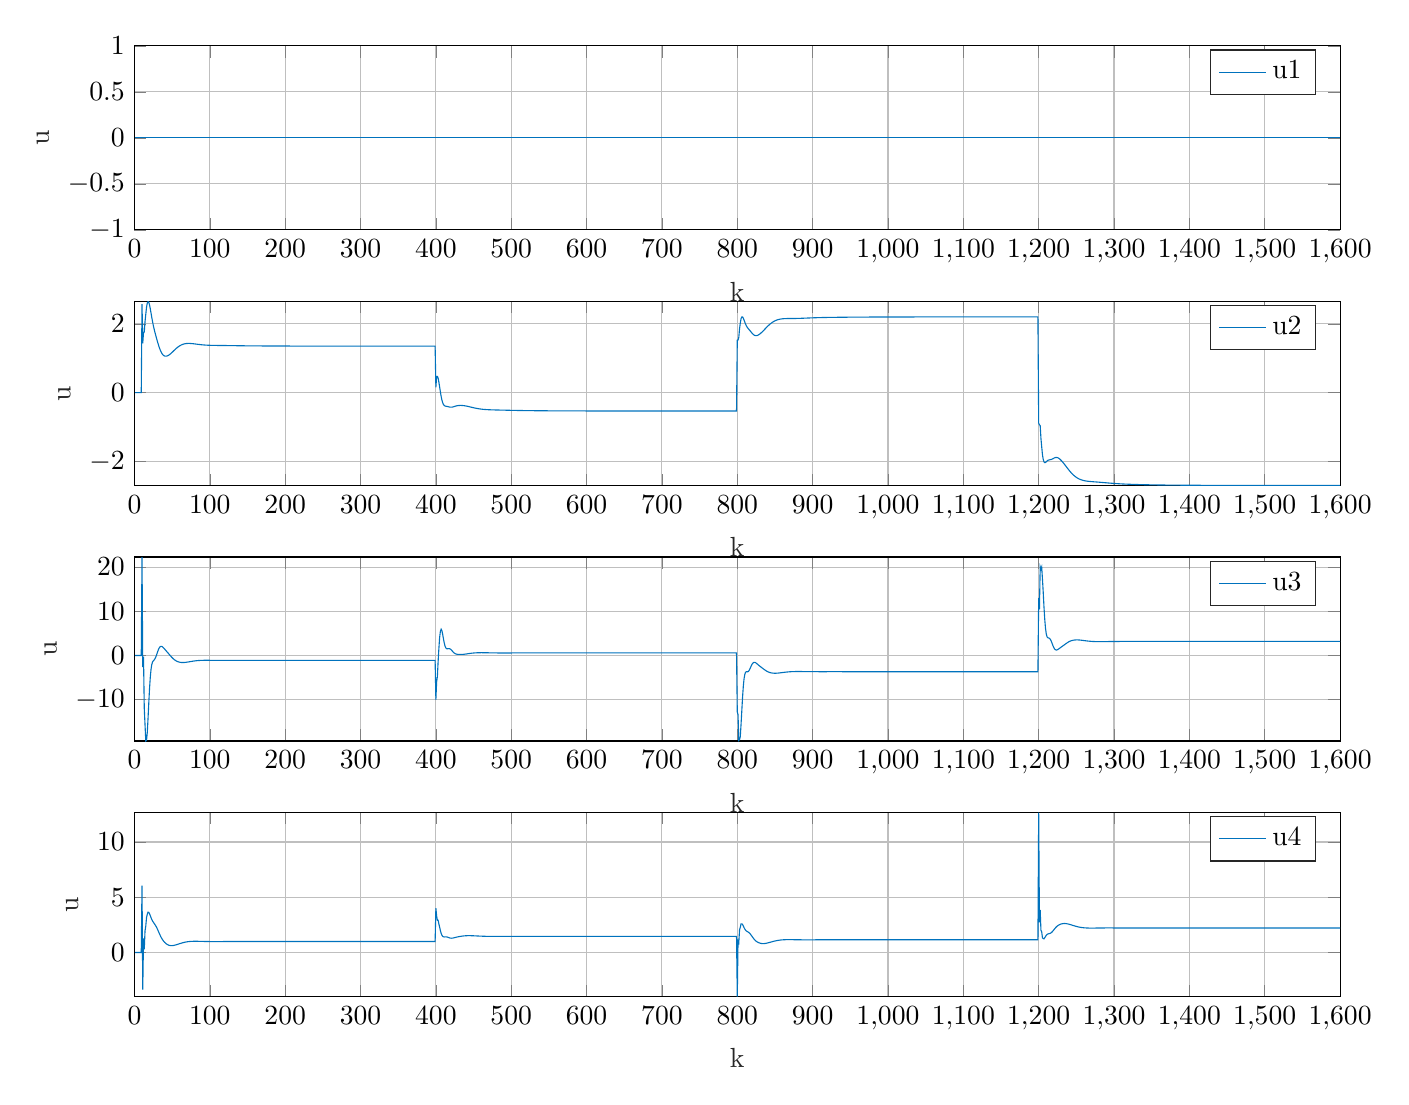
\begin{tikzpicture}

\begin{axis}[%
width=6.028in,
height=0.92in,
at={(1.011in,4.476in)},
scale only axis,
xmin=0,
xmax=1600,
xlabel style={font=\color{white!15!black}},
xlabel={k},
ymin=-1,
ymax=1,
ylabel style={font=\color{white!15!black}},
ylabel={u},
axis background/.style={fill=white},
xmajorgrids,
ymajorgrids,
legend style={legend cell align=left, align=left, draw=white!15!black}
]
\addplot [color=mycolor1]
  table[row sep=crcr]{%
1	0\\
2	0\\
3	0\\
4	0\\
5	0\\
6	0\\
7	0\\
8	0\\
9	0\\
10	0\\
11	0\\
12	0\\
13	0\\
14	0\\
15	0\\
16	0\\
17	0\\
18	0\\
19	0\\
20	0\\
21	0\\
22	0\\
23	0\\
24	0\\
25	0\\
26	0\\
27	0\\
28	0\\
29	0\\
30	0\\
31	0\\
32	0\\
33	0\\
34	0\\
35	0\\
36	0\\
37	0\\
38	0\\
39	0\\
40	0\\
41	0\\
42	0\\
43	0\\
44	0\\
45	0\\
46	0\\
47	0\\
48	0\\
49	0\\
50	0\\
51	0\\
52	0\\
53	0\\
54	0\\
55	0\\
56	0\\
57	0\\
58	0\\
59	0\\
60	0\\
61	0\\
62	0\\
63	0\\
64	0\\
65	0\\
66	0\\
67	0\\
68	0\\
69	0\\
70	0\\
71	0\\
72	0\\
73	0\\
74	0\\
75	0\\
76	0\\
77	0\\
78	0\\
79	0\\
80	0\\
81	0\\
82	0\\
83	0\\
84	0\\
85	0\\
86	0\\
87	0\\
88	0\\
89	0\\
90	0\\
91	0\\
92	0\\
93	0\\
94	0\\
95	0\\
96	0\\
97	0\\
98	0\\
99	0\\
100	0\\
101	0\\
102	0\\
103	0\\
104	0\\
105	0\\
106	0\\
107	0\\
108	0\\
109	0\\
110	0\\
111	0\\
112	0\\
113	0\\
114	0\\
115	0\\
116	0\\
117	0\\
118	0\\
119	0\\
120	0\\
121	0\\
122	0\\
123	0\\
124	0\\
125	0\\
126	0\\
127	0\\
128	0\\
129	0\\
130	0\\
131	0\\
132	0\\
133	0\\
134	0\\
135	0\\
136	0\\
137	0\\
138	0\\
139	0\\
140	0\\
141	0\\
142	0\\
143	0\\
144	0\\
145	0\\
146	0\\
147	0\\
148	0\\
149	0\\
150	0\\
151	0\\
152	0\\
153	0\\
154	0\\
155	0\\
156	0\\
157	0\\
158	0\\
159	0\\
160	0\\
161	0\\
162	0\\
163	0\\
164	0\\
165	0\\
166	0\\
167	0\\
168	0\\
169	0\\
170	0\\
171	0\\
172	0\\
173	0\\
174	0\\
175	0\\
176	0\\
177	0\\
178	0\\
179	0\\
180	0\\
181	0\\
182	0\\
183	0\\
184	0\\
185	0\\
186	0\\
187	0\\
188	0\\
189	0\\
190	0\\
191	0\\
192	0\\
193	0\\
194	0\\
195	0\\
196	0\\
197	0\\
198	0\\
199	0\\
200	0\\
201	0\\
202	0\\
203	0\\
204	0\\
205	0\\
206	0\\
207	0\\
208	0\\
209	0\\
210	0\\
211	0\\
212	0\\
213	0\\
214	0\\
215	0\\
216	0\\
217	0\\
218	0\\
219	0\\
220	0\\
221	0\\
222	0\\
223	0\\
224	0\\
225	0\\
226	0\\
227	0\\
228	0\\
229	0\\
230	0\\
231	0\\
232	0\\
233	0\\
234	0\\
235	0\\
236	0\\
237	0\\
238	0\\
239	0\\
240	0\\
241	0\\
242	0\\
243	0\\
244	0\\
245	0\\
246	0\\
247	0\\
248	0\\
249	0\\
250	0\\
251	0\\
252	0\\
253	0\\
254	0\\
255	0\\
256	0\\
257	0\\
258	0\\
259	0\\
260	0\\
261	0\\
262	0\\
263	0\\
264	0\\
265	0\\
266	0\\
267	0\\
268	0\\
269	0\\
270	0\\
271	0\\
272	0\\
273	0\\
274	0\\
275	0\\
276	0\\
277	0\\
278	0\\
279	0\\
280	0\\
281	0\\
282	0\\
283	0\\
284	0\\
285	0\\
286	0\\
287	0\\
288	0\\
289	0\\
290	0\\
291	0\\
292	0\\
293	0\\
294	0\\
295	0\\
296	0\\
297	0\\
298	0\\
299	0\\
300	0\\
301	0\\
302	0\\
303	0\\
304	0\\
305	0\\
306	0\\
307	0\\
308	0\\
309	0\\
310	0\\
311	0\\
312	0\\
313	0\\
314	0\\
315	0\\
316	0\\
317	0\\
318	0\\
319	0\\
320	0\\
321	0\\
322	0\\
323	0\\
324	0\\
325	0\\
326	0\\
327	0\\
328	0\\
329	0\\
330	0\\
331	0\\
332	0\\
333	0\\
334	0\\
335	0\\
336	0\\
337	0\\
338	0\\
339	0\\
340	0\\
341	0\\
342	0\\
343	0\\
344	0\\
345	0\\
346	0\\
347	0\\
348	0\\
349	0\\
350	0\\
351	0\\
352	0\\
353	0\\
354	0\\
355	0\\
356	0\\
357	0\\
358	0\\
359	0\\
360	0\\
361	0\\
362	0\\
363	0\\
364	0\\
365	0\\
366	0\\
367	0\\
368	0\\
369	0\\
370	0\\
371	0\\
372	0\\
373	0\\
374	0\\
375	0\\
376	0\\
377	0\\
378	0\\
379	0\\
380	0\\
381	0\\
382	0\\
383	0\\
384	0\\
385	0\\
386	0\\
387	0\\
388	0\\
389	0\\
390	0\\
391	0\\
392	0\\
393	0\\
394	0\\
395	0\\
396	0\\
397	0\\
398	0\\
399	0\\
400	0\\
401	0\\
402	0\\
403	0\\
404	0\\
405	0\\
406	0\\
407	0\\
408	0\\
409	0\\
410	0\\
411	0\\
412	0\\
413	0\\
414	0\\
415	0\\
416	0\\
417	0\\
418	0\\
419	0\\
420	0\\
421	0\\
422	0\\
423	0\\
424	0\\
425	0\\
426	0\\
427	0\\
428	0\\
429	0\\
430	0\\
431	0\\
432	0\\
433	0\\
434	0\\
435	0\\
436	0\\
437	0\\
438	0\\
439	0\\
440	0\\
441	0\\
442	0\\
443	0\\
444	0\\
445	0\\
446	0\\
447	0\\
448	0\\
449	0\\
450	0\\
451	0\\
452	0\\
453	0\\
454	0\\
455	0\\
456	0\\
457	0\\
458	0\\
459	0\\
460	0\\
461	0\\
462	0\\
463	0\\
464	0\\
465	0\\
466	0\\
467	0\\
468	0\\
469	0\\
470	0\\
471	0\\
472	0\\
473	0\\
474	0\\
475	0\\
476	0\\
477	0\\
478	0\\
479	0\\
480	0\\
481	0\\
482	0\\
483	0\\
484	0\\
485	0\\
486	0\\
487	0\\
488	0\\
489	0\\
490	0\\
491	0\\
492	0\\
493	0\\
494	0\\
495	0\\
496	0\\
497	0\\
498	0\\
499	0\\
500	0\\
501	0\\
502	0\\
503	0\\
504	0\\
505	0\\
506	0\\
507	0\\
508	0\\
509	0\\
510	0\\
511	0\\
512	0\\
513	0\\
514	0\\
515	0\\
516	0\\
517	0\\
518	0\\
519	0\\
520	0\\
521	0\\
522	0\\
523	0\\
524	0\\
525	0\\
526	0\\
527	0\\
528	0\\
529	0\\
530	0\\
531	0\\
532	0\\
533	0\\
534	0\\
535	0\\
536	0\\
537	0\\
538	0\\
539	0\\
540	0\\
541	0\\
542	0\\
543	0\\
544	0\\
545	0\\
546	0\\
547	0\\
548	0\\
549	0\\
550	0\\
551	0\\
552	0\\
553	0\\
554	0\\
555	0\\
556	0\\
557	0\\
558	0\\
559	0\\
560	0\\
561	0\\
562	0\\
563	0\\
564	0\\
565	0\\
566	0\\
567	0\\
568	0\\
569	0\\
570	0\\
571	0\\
572	0\\
573	0\\
574	0\\
575	0\\
576	0\\
577	0\\
578	0\\
579	0\\
580	0\\
581	0\\
582	0\\
583	0\\
584	0\\
585	0\\
586	0\\
587	0\\
588	0\\
589	0\\
590	0\\
591	0\\
592	0\\
593	0\\
594	0\\
595	0\\
596	0\\
597	0\\
598	0\\
599	0\\
600	0\\
601	0\\
602	0\\
603	0\\
604	0\\
605	0\\
606	0\\
607	0\\
608	0\\
609	0\\
610	0\\
611	0\\
612	0\\
613	0\\
614	0\\
615	0\\
616	0\\
617	0\\
618	0\\
619	0\\
620	0\\
621	0\\
622	0\\
623	0\\
624	0\\
625	0\\
626	0\\
627	0\\
628	0\\
629	0\\
630	0\\
631	0\\
632	0\\
633	0\\
634	0\\
635	0\\
636	0\\
637	0\\
638	0\\
639	0\\
640	0\\
641	0\\
642	0\\
643	0\\
644	0\\
645	0\\
646	0\\
647	0\\
648	0\\
649	0\\
650	0\\
651	0\\
652	0\\
653	0\\
654	0\\
655	0\\
656	0\\
657	0\\
658	0\\
659	0\\
660	0\\
661	0\\
662	0\\
663	0\\
664	0\\
665	0\\
666	0\\
667	0\\
668	0\\
669	0\\
670	0\\
671	0\\
672	0\\
673	0\\
674	0\\
675	0\\
676	0\\
677	0\\
678	0\\
679	0\\
680	0\\
681	0\\
682	0\\
683	0\\
684	0\\
685	0\\
686	0\\
687	0\\
688	0\\
689	0\\
690	0\\
691	0\\
692	0\\
693	0\\
694	0\\
695	0\\
696	0\\
697	0\\
698	0\\
699	0\\
700	0\\
701	0\\
702	0\\
703	0\\
704	0\\
705	0\\
706	0\\
707	0\\
708	0\\
709	0\\
710	0\\
711	0\\
712	0\\
713	0\\
714	0\\
715	0\\
716	0\\
717	0\\
718	0\\
719	0\\
720	0\\
721	0\\
722	0\\
723	0\\
724	0\\
725	0\\
726	0\\
727	0\\
728	0\\
729	0\\
730	0\\
731	0\\
732	0\\
733	0\\
734	0\\
735	0\\
736	0\\
737	0\\
738	0\\
739	0\\
740	0\\
741	0\\
742	0\\
743	0\\
744	0\\
745	0\\
746	0\\
747	0\\
748	0\\
749	0\\
750	0\\
751	0\\
752	0\\
753	0\\
754	0\\
755	0\\
756	0\\
757	0\\
758	0\\
759	0\\
760	0\\
761	0\\
762	0\\
763	0\\
764	0\\
765	0\\
766	0\\
767	0\\
768	0\\
769	0\\
770	0\\
771	0\\
772	0\\
773	0\\
774	0\\
775	0\\
776	0\\
777	0\\
778	0\\
779	0\\
780	0\\
781	0\\
782	0\\
783	0\\
784	0\\
785	0\\
786	0\\
787	0\\
788	0\\
789	0\\
790	0\\
791	0\\
792	0\\
793	0\\
794	0\\
795	0\\
796	0\\
797	0\\
798	0\\
799	0\\
800	0\\
801	0\\
802	0\\
803	0\\
804	0\\
805	0\\
806	0\\
807	0\\
808	0\\
809	0\\
810	0\\
811	0\\
812	0\\
813	0\\
814	0\\
815	0\\
816	0\\
817	0\\
818	0\\
819	0\\
820	0\\
821	0\\
822	0\\
823	0\\
824	0\\
825	0\\
826	0\\
827	0\\
828	0\\
829	0\\
830	0\\
831	0\\
832	0\\
833	0\\
834	0\\
835	0\\
836	0\\
837	0\\
838	0\\
839	0\\
840	0\\
841	0\\
842	0\\
843	0\\
844	0\\
845	0\\
846	0\\
847	0\\
848	0\\
849	0\\
850	0\\
851	0\\
852	0\\
853	0\\
854	0\\
855	0\\
856	0\\
857	0\\
858	0\\
859	0\\
860	0\\
861	0\\
862	0\\
863	0\\
864	0\\
865	0\\
866	0\\
867	0\\
868	0\\
869	0\\
870	0\\
871	0\\
872	0\\
873	0\\
874	0\\
875	0\\
876	0\\
877	0\\
878	0\\
879	0\\
880	0\\
881	0\\
882	0\\
883	0\\
884	0\\
885	0\\
886	0\\
887	0\\
888	0\\
889	0\\
890	0\\
891	0\\
892	0\\
893	0\\
894	0\\
895	0\\
896	0\\
897	0\\
898	0\\
899	0\\
900	0\\
901	0\\
902	0\\
903	0\\
904	0\\
905	0\\
906	0\\
907	0\\
908	0\\
909	0\\
910	0\\
911	0\\
912	0\\
913	0\\
914	0\\
915	0\\
916	0\\
917	0\\
918	0\\
919	0\\
920	0\\
921	0\\
922	0\\
923	0\\
924	0\\
925	0\\
926	0\\
927	0\\
928	0\\
929	0\\
930	0\\
931	0\\
932	0\\
933	0\\
934	0\\
935	0\\
936	0\\
937	0\\
938	0\\
939	0\\
940	0\\
941	0\\
942	0\\
943	0\\
944	0\\
945	0\\
946	0\\
947	0\\
948	0\\
949	0\\
950	0\\
951	0\\
952	0\\
953	0\\
954	0\\
955	0\\
956	0\\
957	0\\
958	0\\
959	0\\
960	0\\
961	0\\
962	0\\
963	0\\
964	0\\
965	0\\
966	0\\
967	0\\
968	0\\
969	0\\
970	0\\
971	0\\
972	0\\
973	0\\
974	0\\
975	0\\
976	0\\
977	0\\
978	0\\
979	0\\
980	0\\
981	0\\
982	0\\
983	0\\
984	0\\
985	0\\
986	0\\
987	0\\
988	0\\
989	0\\
990	0\\
991	0\\
992	0\\
993	0\\
994	0\\
995	0\\
996	0\\
997	0\\
998	0\\
999	0\\
1000	0\\
1001	0\\
1002	0\\
1003	0\\
1004	0\\
1005	0\\
1006	0\\
1007	0\\
1008	0\\
1009	0\\
1010	0\\
1011	0\\
1012	0\\
1013	0\\
1014	0\\
1015	0\\
1016	0\\
1017	0\\
1018	0\\
1019	0\\
1020	0\\
1021	0\\
1022	0\\
1023	0\\
1024	0\\
1025	0\\
1026	0\\
1027	0\\
1028	0\\
1029	0\\
1030	0\\
1031	0\\
1032	0\\
1033	0\\
1034	0\\
1035	0\\
1036	0\\
1037	0\\
1038	0\\
1039	0\\
1040	0\\
1041	0\\
1042	0\\
1043	0\\
1044	0\\
1045	0\\
1046	0\\
1047	0\\
1048	0\\
1049	0\\
1050	0\\
1051	0\\
1052	0\\
1053	0\\
1054	0\\
1055	0\\
1056	0\\
1057	0\\
1058	0\\
1059	0\\
1060	0\\
1061	0\\
1062	0\\
1063	0\\
1064	0\\
1065	0\\
1066	0\\
1067	0\\
1068	0\\
1069	0\\
1070	0\\
1071	0\\
1072	0\\
1073	0\\
1074	0\\
1075	0\\
1076	0\\
1077	0\\
1078	0\\
1079	0\\
1080	0\\
1081	0\\
1082	0\\
1083	0\\
1084	0\\
1085	0\\
1086	0\\
1087	0\\
1088	0\\
1089	0\\
1090	0\\
1091	0\\
1092	0\\
1093	0\\
1094	0\\
1095	0\\
1096	0\\
1097	0\\
1098	0\\
1099	0\\
1100	0\\
1101	0\\
1102	0\\
1103	0\\
1104	0\\
1105	0\\
1106	0\\
1107	0\\
1108	0\\
1109	0\\
1110	0\\
1111	0\\
1112	0\\
1113	0\\
1114	0\\
1115	0\\
1116	0\\
1117	0\\
1118	0\\
1119	0\\
1120	0\\
1121	0\\
1122	0\\
1123	0\\
1124	0\\
1125	0\\
1126	0\\
1127	0\\
1128	0\\
1129	0\\
1130	0\\
1131	0\\
1132	0\\
1133	0\\
1134	0\\
1135	0\\
1136	0\\
1137	0\\
1138	0\\
1139	0\\
1140	0\\
1141	0\\
1142	0\\
1143	0\\
1144	0\\
1145	0\\
1146	0\\
1147	0\\
1148	0\\
1149	0\\
1150	0\\
1151	0\\
1152	0\\
1153	0\\
1154	0\\
1155	0\\
1156	0\\
1157	0\\
1158	0\\
1159	0\\
1160	0\\
1161	0\\
1162	0\\
1163	0\\
1164	0\\
1165	0\\
1166	0\\
1167	0\\
1168	0\\
1169	0\\
1170	0\\
1171	0\\
1172	0\\
1173	0\\
1174	0\\
1175	0\\
1176	0\\
1177	0\\
1178	0\\
1179	0\\
1180	0\\
1181	0\\
1182	0\\
1183	0\\
1184	0\\
1185	0\\
1186	0\\
1187	0\\
1188	0\\
1189	0\\
1190	0\\
1191	0\\
1192	0\\
1193	0\\
1194	0\\
1195	0\\
1196	0\\
1197	0\\
1198	0\\
1199	0\\
1200	0\\
1201	0\\
1202	0\\
1203	0\\
1204	0\\
1205	0\\
1206	0\\
1207	0\\
1208	0\\
1209	0\\
1210	0\\
1211	0\\
1212	0\\
1213	0\\
1214	0\\
1215	0\\
1216	0\\
1217	0\\
1218	0\\
1219	0\\
1220	0\\
1221	0\\
1222	0\\
1223	0\\
1224	0\\
1225	0\\
1226	0\\
1227	0\\
1228	0\\
1229	0\\
1230	0\\
1231	0\\
1232	0\\
1233	0\\
1234	0\\
1235	0\\
1236	0\\
1237	0\\
1238	0\\
1239	0\\
1240	0\\
1241	0\\
1242	0\\
1243	0\\
1244	0\\
1245	0\\
1246	0\\
1247	0\\
1248	0\\
1249	0\\
1250	0\\
1251	0\\
1252	0\\
1253	0\\
1254	0\\
1255	0\\
1256	0\\
1257	0\\
1258	0\\
1259	0\\
1260	0\\
1261	0\\
1262	0\\
1263	0\\
1264	0\\
1265	0\\
1266	0\\
1267	0\\
1268	0\\
1269	0\\
1270	0\\
1271	0\\
1272	0\\
1273	0\\
1274	0\\
1275	0\\
1276	0\\
1277	0\\
1278	0\\
1279	0\\
1280	0\\
1281	0\\
1282	0\\
1283	0\\
1284	0\\
1285	0\\
1286	0\\
1287	0\\
1288	0\\
1289	0\\
1290	0\\
1291	0\\
1292	0\\
1293	0\\
1294	0\\
1295	0\\
1296	0\\
1297	0\\
1298	0\\
1299	0\\
1300	0\\
1301	0\\
1302	0\\
1303	0\\
1304	0\\
1305	0\\
1306	0\\
1307	0\\
1308	0\\
1309	0\\
1310	0\\
1311	0\\
1312	0\\
1313	0\\
1314	0\\
1315	0\\
1316	0\\
1317	0\\
1318	0\\
1319	0\\
1320	0\\
1321	0\\
1322	0\\
1323	0\\
1324	0\\
1325	0\\
1326	0\\
1327	0\\
1328	0\\
1329	0\\
1330	0\\
1331	0\\
1332	0\\
1333	0\\
1334	0\\
1335	0\\
1336	0\\
1337	0\\
1338	0\\
1339	0\\
1340	0\\
1341	0\\
1342	0\\
1343	0\\
1344	0\\
1345	0\\
1346	0\\
1347	0\\
1348	0\\
1349	0\\
1350	0\\
1351	0\\
1352	0\\
1353	0\\
1354	0\\
1355	0\\
1356	0\\
1357	0\\
1358	0\\
1359	0\\
1360	0\\
1361	0\\
1362	0\\
1363	0\\
1364	0\\
1365	0\\
1366	0\\
1367	0\\
1368	0\\
1369	0\\
1370	0\\
1371	0\\
1372	0\\
1373	0\\
1374	0\\
1375	0\\
1376	0\\
1377	0\\
1378	0\\
1379	0\\
1380	0\\
1381	0\\
1382	0\\
1383	0\\
1384	0\\
1385	0\\
1386	0\\
1387	0\\
1388	0\\
1389	0\\
1390	0\\
1391	0\\
1392	0\\
1393	0\\
1394	0\\
1395	0\\
1396	0\\
1397	0\\
1398	0\\
1399	0\\
1400	0\\
1401	0\\
1402	0\\
1403	0\\
1404	0\\
1405	0\\
1406	0\\
1407	0\\
1408	0\\
1409	0\\
1410	0\\
1411	0\\
1412	0\\
1413	0\\
1414	0\\
1415	0\\
1416	0\\
1417	0\\
1418	0\\
1419	0\\
1420	0\\
1421	0\\
1422	0\\
1423	0\\
1424	0\\
1425	0\\
1426	0\\
1427	0\\
1428	0\\
1429	0\\
1430	0\\
1431	0\\
1432	0\\
1433	0\\
1434	0\\
1435	0\\
1436	0\\
1437	0\\
1438	0\\
1439	0\\
1440	0\\
1441	0\\
1442	0\\
1443	0\\
1444	0\\
1445	0\\
1446	0\\
1447	0\\
1448	0\\
1449	0\\
1450	0\\
1451	0\\
1452	0\\
1453	0\\
1454	0\\
1455	0\\
1456	0\\
1457	0\\
1458	0\\
1459	0\\
1460	0\\
1461	0\\
1462	0\\
1463	0\\
1464	0\\
1465	0\\
1466	0\\
1467	0\\
1468	0\\
1469	0\\
1470	0\\
1471	0\\
1472	0\\
1473	0\\
1474	0\\
1475	0\\
1476	0\\
1477	0\\
1478	0\\
1479	0\\
1480	0\\
1481	0\\
1482	0\\
1483	0\\
1484	0\\
1485	0\\
1486	0\\
1487	0\\
1488	0\\
1489	0\\
1490	0\\
1491	0\\
1492	0\\
1493	0\\
1494	0\\
1495	0\\
1496	0\\
1497	0\\
1498	0\\
1499	0\\
1500	0\\
1501	0\\
1502	0\\
1503	0\\
1504	0\\
1505	0\\
1506	0\\
1507	0\\
1508	0\\
1509	0\\
1510	0\\
1511	0\\
1512	0\\
1513	0\\
1514	0\\
1515	0\\
1516	0\\
1517	0\\
1518	0\\
1519	0\\
1520	0\\
1521	0\\
1522	0\\
1523	0\\
1524	0\\
1525	0\\
1526	0\\
1527	0\\
1528	0\\
1529	0\\
1530	0\\
1531	0\\
1532	0\\
1533	0\\
1534	0\\
1535	0\\
1536	0\\
1537	0\\
1538	0\\
1539	0\\
1540	0\\
1541	0\\
1542	0\\
1543	0\\
1544	0\\
1545	0\\
1546	0\\
1547	0\\
1548	0\\
1549	0\\
1550	0\\
1551	0\\
1552	0\\
1553	0\\
1554	0\\
1555	0\\
1556	0\\
1557	0\\
1558	0\\
1559	0\\
1560	0\\
1561	0\\
1562	0\\
1563	0\\
1564	0\\
1565	0\\
1566	0\\
1567	0\\
1568	0\\
1569	0\\
1570	0\\
1571	0\\
1572	0\\
1573	0\\
1574	0\\
1575	0\\
1576	0\\
1577	0\\
1578	0\\
1579	0\\
1580	0\\
1581	0\\
1582	0\\
1583	0\\
1584	0\\
1585	0\\
1586	0\\
1587	0\\
1588	0\\
1589	0\\
1590	0\\
1591	0\\
1592	0\\
1593	0\\
1594	0\\
1595	0\\
1596	0\\
1597	0\\
1598	0\\
1599	0\\
1600	0\\
};
\addlegendentry{u1}

\end{axis}

\begin{axis}[%
width=6.028in,
height=0.92in,
at={(1.011in,3.198in)},
scale only axis,
xmin=0,
xmax=1600,
xlabel style={font=\color{white!15!black}},
xlabel={k},
ymin=-2.7028,
ymax=2.6543,
ylabel style={font=\color{white!15!black}},
ylabel={u},
axis background/.style={fill=white},
xmajorgrids,
ymajorgrids,
legend style={legend cell align=left, align=left, draw=white!15!black}
]
\addplot [color=mycolor1]
  table[row sep=crcr]{%
1	0\\
2	0\\
3	0\\
4	0\\
5	0\\
6	0\\
7	0\\
8	0\\
9	0\\
10	2.5762\\
11	1.4334\\
12	1.7475\\
13	1.7623\\
14	2.0627\\
15	2.2759\\
16	2.4855\\
17	2.6054\\
18	2.6543\\
19	2.6286\\
20	2.5507\\
21	2.4386\\
22	2.3121\\
23	2.1845\\
24	2.0647\\
25	1.9559\\
26	1.8577\\
27	1.7679\\
28	1.6837\\
29	1.603\\
30	1.5248\\
31	1.4491\\
32	1.3772\\
33	1.3104\\
34	1.2504\\
35	1.1984\\
36	1.155\\
37	1.1205\\
38	1.0944\\
39	1.0761\\
40	1.0648\\
41	1.0596\\
42	1.0595\\
43	1.0639\\
44	1.072\\
45	1.0833\\
46	1.0974\\
47	1.1137\\
48	1.1319\\
49	1.1515\\
50	1.1722\\
51	1.1934\\
52	1.2148\\
53	1.2361\\
54	1.2568\\
55	1.2769\\
56	1.2961\\
57	1.3141\\
58	1.3309\\
59	1.3464\\
60	1.3605\\
61	1.3733\\
62	1.3846\\
63	1.3946\\
64	1.4032\\
65	1.4106\\
66	1.4167\\
67	1.4216\\
68	1.4254\\
69	1.4282\\
70	1.43\\
71	1.4311\\
72	1.4313\\
73	1.431\\
74	1.43\\
75	1.4286\\
76	1.4267\\
77	1.4246\\
78	1.4221\\
79	1.4195\\
80	1.4167\\
81	1.4139\\
82	1.411\\
83	1.4081\\
84	1.4053\\
85	1.4025\\
86	1.3998\\
87	1.3972\\
88	1.3948\\
89	1.3924\\
90	1.3903\\
91	1.3883\\
92	1.3864\\
93	1.3847\\
94	1.3832\\
95	1.3817\\
96	1.3805\\
97	1.3793\\
98	1.3783\\
99	1.3774\\
100	1.3766\\
101	1.3759\\
102	1.3753\\
103	1.3747\\
104	1.3742\\
105	1.3738\\
106	1.3734\\
107	1.3731\\
108	1.3728\\
109	1.3725\\
110	1.3722\\
111	1.372\\
112	1.3717\\
113	1.3715\\
114	1.3713\\
115	1.371\\
116	1.3708\\
117	1.3706\\
118	1.3703\\
119	1.3701\\
120	1.3698\\
121	1.3695\\
122	1.3692\\
123	1.369\\
124	1.3687\\
125	1.3684\\
126	1.368\\
127	1.3677\\
128	1.3674\\
129	1.3671\\
130	1.3668\\
131	1.3664\\
132	1.3661\\
133	1.3658\\
134	1.3655\\
135	1.3651\\
136	1.3648\\
137	1.3645\\
138	1.3642\\
139	1.3639\\
140	1.3636\\
141	1.3633\\
142	1.363\\
143	1.3627\\
144	1.3625\\
145	1.3622\\
146	1.3619\\
147	1.3617\\
148	1.3614\\
149	1.3612\\
150	1.361\\
151	1.3607\\
152	1.3605\\
153	1.3603\\
154	1.3601\\
155	1.3599\\
156	1.3597\\
157	1.3596\\
158	1.3594\\
159	1.3592\\
160	1.359\\
161	1.3589\\
162	1.3587\\
163	1.3586\\
164	1.3584\\
165	1.3583\\
166	1.3581\\
167	1.358\\
168	1.3579\\
169	1.3577\\
170	1.3576\\
171	1.3575\\
172	1.3574\\
173	1.3572\\
174	1.3571\\
175	1.357\\
176	1.3569\\
177	1.3568\\
178	1.3567\\
179	1.3566\\
180	1.3565\\
181	1.3564\\
182	1.3563\\
183	1.3562\\
184	1.3561\\
185	1.356\\
186	1.356\\
187	1.3559\\
188	1.3558\\
189	1.3557\\
190	1.3556\\
191	1.3555\\
192	1.3555\\
193	1.3554\\
194	1.3553\\
195	1.3553\\
196	1.3552\\
197	1.3551\\
198	1.3551\\
199	1.355\\
200	1.3549\\
201	1.3549\\
202	1.3548\\
203	1.3548\\
204	1.3547\\
205	1.3546\\
206	1.3546\\
207	1.3545\\
208	1.3545\\
209	1.3544\\
210	1.3544\\
211	1.3543\\
212	1.3543\\
213	1.3543\\
214	1.3542\\
215	1.3542\\
216	1.3541\\
217	1.3541\\
218	1.354\\
219	1.354\\
220	1.354\\
221	1.3539\\
222	1.3539\\
223	1.3539\\
224	1.3538\\
225	1.3538\\
226	1.3538\\
227	1.3537\\
228	1.3537\\
229	1.3537\\
230	1.3536\\
231	1.3536\\
232	1.3536\\
233	1.3536\\
234	1.3535\\
235	1.3535\\
236	1.3535\\
237	1.3535\\
238	1.3534\\
239	1.3534\\
240	1.3534\\
241	1.3534\\
242	1.3533\\
243	1.3533\\
244	1.3533\\
245	1.3533\\
246	1.3533\\
247	1.3532\\
248	1.3532\\
249	1.3532\\
250	1.3532\\
251	1.3532\\
252	1.3532\\
253	1.3531\\
254	1.3531\\
255	1.3531\\
256	1.3531\\
257	1.3531\\
258	1.3531\\
259	1.353\\
260	1.353\\
261	1.353\\
262	1.353\\
263	1.353\\
264	1.353\\
265	1.353\\
266	1.353\\
267	1.3529\\
268	1.3529\\
269	1.3529\\
270	1.3529\\
271	1.3529\\
272	1.3529\\
273	1.3529\\
274	1.3529\\
275	1.3529\\
276	1.3528\\
277	1.3528\\
278	1.3528\\
279	1.3528\\
280	1.3528\\
281	1.3528\\
282	1.3528\\
283	1.3528\\
284	1.3528\\
285	1.3528\\
286	1.3528\\
287	1.3528\\
288	1.3528\\
289	1.3527\\
290	1.3527\\
291	1.3527\\
292	1.3527\\
293	1.3527\\
294	1.3527\\
295	1.3527\\
296	1.3527\\
297	1.3527\\
298	1.3527\\
299	1.3527\\
300	1.3527\\
301	1.3527\\
302	1.3527\\
303	1.3527\\
304	1.3527\\
305	1.3527\\
306	1.3527\\
307	1.3527\\
308	1.3526\\
309	1.3526\\
310	1.3526\\
311	1.3526\\
312	1.3526\\
313	1.3526\\
314	1.3526\\
315	1.3526\\
316	1.3526\\
317	1.3526\\
318	1.3526\\
319	1.3526\\
320	1.3526\\
321	1.3526\\
322	1.3526\\
323	1.3526\\
324	1.3526\\
325	1.3526\\
326	1.3526\\
327	1.3526\\
328	1.3526\\
329	1.3526\\
330	1.3526\\
331	1.3526\\
332	1.3526\\
333	1.3526\\
334	1.3526\\
335	1.3526\\
336	1.3526\\
337	1.3526\\
338	1.3526\\
339	1.3526\\
340	1.3526\\
341	1.3526\\
342	1.3526\\
343	1.3525\\
344	1.3525\\
345	1.3525\\
346	1.3525\\
347	1.3525\\
348	1.3525\\
349	1.3525\\
350	1.3525\\
351	1.3525\\
352	1.3525\\
353	1.3525\\
354	1.3525\\
355	1.3525\\
356	1.3525\\
357	1.3525\\
358	1.3525\\
359	1.3525\\
360	1.3525\\
361	1.3525\\
362	1.3525\\
363	1.3525\\
364	1.3525\\
365	1.3525\\
366	1.3525\\
367	1.3525\\
368	1.3525\\
369	1.3525\\
370	1.3525\\
371	1.3525\\
372	1.3525\\
373	1.3525\\
374	1.3525\\
375	1.3525\\
376	1.3525\\
377	1.3525\\
378	1.3525\\
379	1.3525\\
380	1.3525\\
381	1.3525\\
382	1.3525\\
383	1.3525\\
384	1.3525\\
385	1.3525\\
386	1.3525\\
387	1.3525\\
388	1.3525\\
389	1.3525\\
390	1.3525\\
391	1.3525\\
392	1.3525\\
393	1.3525\\
394	1.3525\\
395	1.3525\\
396	1.3525\\
397	1.3525\\
398	1.3525\\
399	1.3525\\
400	0.15025\\
401	0.46918\\
402	0.46953\\
403	0.42304\\
404	0.30264\\
405	0.16359\\
406	0.017807\\
407	-0.11177\\
408	-0.217\\
409	-0.29345\\
410	-0.3437\\
411	-0.37308\\
412	-0.38845\\
413	-0.39604\\
414	-0.40058\\
415	-0.40485\\
416	-0.40986\\
417	-0.41536\\
418	-0.42042\\
419	-0.42402\\
420	-0.42539\\
421	-0.42421\\
422	-0.42064\\
423	-0.4152\\
424	-0.4086\\
425	-0.4016\\
426	-0.39484\\
427	-0.3888\\
428	-0.38376\\
429	-0.37983\\
430	-0.37701\\
431	-0.3752\\
432	-0.37428\\
433	-0.37414\\
434	-0.37471\\
435	-0.37593\\
436	-0.37776\\
437	-0.38018\\
438	-0.38315\\
439	-0.38665\\
440	-0.39062\\
441	-0.395\\
442	-0.39973\\
443	-0.40472\\
444	-0.4099\\
445	-0.4152\\
446	-0.42055\\
447	-0.42588\\
448	-0.43117\\
449	-0.43636\\
450	-0.44141\\
451	-0.44631\\
452	-0.45103\\
453	-0.45555\\
454	-0.45986\\
455	-0.46393\\
456	-0.46777\\
457	-0.47137\\
458	-0.47473\\
459	-0.47786\\
460	-0.48074\\
461	-0.4834\\
462	-0.48584\\
463	-0.48808\\
464	-0.49012\\
465	-0.49198\\
466	-0.49366\\
467	-0.4952\\
468	-0.49658\\
469	-0.49784\\
470	-0.49899\\
471	-0.50003\\
472	-0.50097\\
473	-0.50184\\
474	-0.50264\\
475	-0.50338\\
476	-0.50406\\
477	-0.50471\\
478	-0.50532\\
479	-0.5059\\
480	-0.50646\\
481	-0.507\\
482	-0.50753\\
483	-0.50805\\
484	-0.50856\\
485	-0.50907\\
486	-0.50958\\
487	-0.51008\\
488	-0.51059\\
489	-0.5111\\
490	-0.51161\\
491	-0.51212\\
492	-0.51263\\
493	-0.51314\\
494	-0.51365\\
495	-0.51417\\
496	-0.51468\\
497	-0.51518\\
498	-0.51569\\
499	-0.51619\\
500	-0.51668\\
501	-0.51717\\
502	-0.51765\\
503	-0.51813\\
504	-0.5186\\
505	-0.51905\\
506	-0.5195\\
507	-0.51994\\
508	-0.52037\\
509	-0.52079\\
510	-0.5212\\
511	-0.5216\\
512	-0.52199\\
513	-0.52236\\
514	-0.52273\\
515	-0.52308\\
516	-0.52343\\
517	-0.52376\\
518	-0.52409\\
519	-0.5244\\
520	-0.52471\\
521	-0.525\\
522	-0.52529\\
523	-0.52557\\
524	-0.52584\\
525	-0.5261\\
526	-0.52635\\
527	-0.5266\\
528	-0.52684\\
529	-0.52707\\
530	-0.5273\\
531	-0.52752\\
532	-0.52773\\
533	-0.52794\\
534	-0.52814\\
535	-0.52834\\
536	-0.52853\\
537	-0.52872\\
538	-0.5289\\
539	-0.52908\\
540	-0.52925\\
541	-0.52942\\
542	-0.52959\\
543	-0.52975\\
544	-0.52991\\
545	-0.53006\\
546	-0.53021\\
547	-0.53036\\
548	-0.5305\\
549	-0.53065\\
550	-0.53078\\
551	-0.53092\\
552	-0.53105\\
553	-0.53118\\
554	-0.5313\\
555	-0.53143\\
556	-0.53155\\
557	-0.53166\\
558	-0.53178\\
559	-0.53189\\
560	-0.532\\
561	-0.5321\\
562	-0.53221\\
563	-0.53231\\
564	-0.53241\\
565	-0.53251\\
566	-0.5326\\
567	-0.53269\\
568	-0.53278\\
569	-0.53287\\
570	-0.53295\\
571	-0.53304\\
572	-0.53312\\
573	-0.5332\\
574	-0.53328\\
575	-0.53335\\
576	-0.53343\\
577	-0.5335\\
578	-0.53357\\
579	-0.53364\\
580	-0.5337\\
581	-0.53377\\
582	-0.53383\\
583	-0.53389\\
584	-0.53395\\
585	-0.53401\\
586	-0.53407\\
587	-0.53412\\
588	-0.53418\\
589	-0.53423\\
590	-0.53428\\
591	-0.53434\\
592	-0.53438\\
593	-0.53443\\
594	-0.53448\\
595	-0.53453\\
596	-0.53457\\
597	-0.53461\\
598	-0.53466\\
599	-0.5347\\
600	-0.53474\\
601	-0.53478\\
602	-0.53482\\
603	-0.53485\\
604	-0.53489\\
605	-0.53493\\
606	-0.53496\\
607	-0.535\\
608	-0.53503\\
609	-0.53506\\
610	-0.53509\\
611	-0.53512\\
612	-0.53516\\
613	-0.53518\\
614	-0.53521\\
615	-0.53524\\
616	-0.53527\\
617	-0.5353\\
618	-0.53532\\
619	-0.53535\\
620	-0.53537\\
621	-0.5354\\
622	-0.53542\\
623	-0.53544\\
624	-0.53546\\
625	-0.53549\\
626	-0.53551\\
627	-0.53553\\
628	-0.53555\\
629	-0.53557\\
630	-0.53559\\
631	-0.53561\\
632	-0.53563\\
633	-0.53564\\
634	-0.53566\\
635	-0.53568\\
636	-0.53569\\
637	-0.53571\\
638	-0.53573\\
639	-0.53574\\
640	-0.53576\\
641	-0.53577\\
642	-0.53579\\
643	-0.5358\\
644	-0.53581\\
645	-0.53583\\
646	-0.53584\\
647	-0.53585\\
648	-0.53587\\
649	-0.53588\\
650	-0.53589\\
651	-0.5359\\
652	-0.53591\\
653	-0.53592\\
654	-0.53593\\
655	-0.53594\\
656	-0.53595\\
657	-0.53596\\
658	-0.53597\\
659	-0.53598\\
660	-0.53599\\
661	-0.536\\
662	-0.53601\\
663	-0.53602\\
664	-0.53603\\
665	-0.53604\\
666	-0.53604\\
667	-0.53605\\
668	-0.53606\\
669	-0.53607\\
670	-0.53607\\
671	-0.53608\\
672	-0.53609\\
673	-0.53609\\
674	-0.5361\\
675	-0.53611\\
676	-0.53611\\
677	-0.53612\\
678	-0.53612\\
679	-0.53613\\
680	-0.53614\\
681	-0.53614\\
682	-0.53615\\
683	-0.53615\\
684	-0.53616\\
685	-0.53616\\
686	-0.53617\\
687	-0.53617\\
688	-0.53618\\
689	-0.53618\\
690	-0.53619\\
691	-0.53619\\
692	-0.53619\\
693	-0.5362\\
694	-0.5362\\
695	-0.53621\\
696	-0.53621\\
697	-0.53621\\
698	-0.53622\\
699	-0.53622\\
700	-0.53622\\
701	-0.53623\\
702	-0.53623\\
703	-0.53623\\
704	-0.53624\\
705	-0.53624\\
706	-0.53624\\
707	-0.53624\\
708	-0.53625\\
709	-0.53625\\
710	-0.53625\\
711	-0.53626\\
712	-0.53626\\
713	-0.53626\\
714	-0.53626\\
715	-0.53627\\
716	-0.53627\\
717	-0.53627\\
718	-0.53627\\
719	-0.53627\\
720	-0.53628\\
721	-0.53628\\
722	-0.53628\\
723	-0.53628\\
724	-0.53628\\
725	-0.53629\\
726	-0.53629\\
727	-0.53629\\
728	-0.53629\\
729	-0.53629\\
730	-0.53629\\
731	-0.5363\\
732	-0.5363\\
733	-0.5363\\
734	-0.5363\\
735	-0.5363\\
736	-0.5363\\
737	-0.53631\\
738	-0.53631\\
739	-0.53631\\
740	-0.53631\\
741	-0.53631\\
742	-0.53631\\
743	-0.53631\\
744	-0.53631\\
745	-0.53631\\
746	-0.53632\\
747	-0.53632\\
748	-0.53632\\
749	-0.53632\\
750	-0.53632\\
751	-0.53632\\
752	-0.53632\\
753	-0.53632\\
754	-0.53632\\
755	-0.53632\\
756	-0.53633\\
757	-0.53633\\
758	-0.53633\\
759	-0.53633\\
760	-0.53633\\
761	-0.53633\\
762	-0.53633\\
763	-0.53633\\
764	-0.53633\\
765	-0.53633\\
766	-0.53633\\
767	-0.53633\\
768	-0.53633\\
769	-0.53633\\
770	-0.53634\\
771	-0.53634\\
772	-0.53634\\
773	-0.53634\\
774	-0.53634\\
775	-0.53634\\
776	-0.53634\\
777	-0.53634\\
778	-0.53634\\
779	-0.53634\\
780	-0.53634\\
781	-0.53634\\
782	-0.53634\\
783	-0.53634\\
784	-0.53634\\
785	-0.53634\\
786	-0.53634\\
787	-0.53634\\
788	-0.53634\\
789	-0.53634\\
790	-0.53634\\
791	-0.53635\\
792	-0.53635\\
793	-0.53635\\
794	-0.53635\\
795	-0.53635\\
796	-0.53635\\
797	-0.53635\\
798	-0.53635\\
799	-0.53635\\
800	1.5247\\
801	1.5302\\
802	1.6066\\
803	1.8568\\
804	2.0218\\
805	2.1499\\
806	2.2016\\
807	2.2036\\
808	2.1663\\
809	2.1109\\
810	2.0502\\
811	1.9943\\
812	1.947\\
813	1.9089\\
814	1.8777\\
815	1.8504\\
816	1.8246\\
817	1.7986\\
818	1.7719\\
819	1.7454\\
820	1.7203\\
821	1.6981\\
822	1.68\\
823	1.667\\
824	1.6594\\
825	1.6572\\
826	1.66\\
827	1.6672\\
828	1.6779\\
829	1.6916\\
830	1.7077\\
831	1.7257\\
832	1.7452\\
833	1.7659\\
834	1.7875\\
835	1.8099\\
836	1.8327\\
837	1.8558\\
838	1.8788\\
839	1.9015\\
840	1.9237\\
841	1.9451\\
842	1.9657\\
843	1.9852\\
844	2.0037\\
845	2.021\\
846	2.037\\
847	2.0518\\
848	2.0654\\
849	2.0778\\
850	2.089\\
851	2.0991\\
852	2.1081\\
853	2.116\\
854	2.123\\
855	2.129\\
856	2.1343\\
857	2.1387\\
858	2.1425\\
859	2.1456\\
860	2.1481\\
861	2.1502\\
862	2.1519\\
863	2.1532\\
864	2.1542\\
865	2.1549\\
866	2.1555\\
867	2.1559\\
868	2.1561\\
869	2.1563\\
870	2.1565\\
871	2.1566\\
872	2.1567\\
873	2.1569\\
874	2.157\\
875	2.1572\\
876	2.1575\\
877	2.1578\\
878	2.1582\\
879	2.1586\\
880	2.1592\\
881	2.1597\\
882	2.1604\\
883	2.1611\\
884	2.1618\\
885	2.1626\\
886	2.1634\\
887	2.1643\\
888	2.1652\\
889	2.1661\\
890	2.167\\
891	2.168\\
892	2.1689\\
893	2.1699\\
894	2.1708\\
895	2.1718\\
896	2.1727\\
897	2.1736\\
898	2.1745\\
899	2.1754\\
900	2.1762\\
901	2.177\\
902	2.1778\\
903	2.1786\\
904	2.1793\\
905	2.18\\
906	2.1807\\
907	2.1814\\
908	2.182\\
909	2.1826\\
910	2.1832\\
911	2.1837\\
912	2.1843\\
913	2.1848\\
914	2.1852\\
915	2.1857\\
916	2.1861\\
917	2.1866\\
918	2.187\\
919	2.1874\\
920	2.1878\\
921	2.1881\\
922	2.1885\\
923	2.1888\\
924	2.1891\\
925	2.1895\\
926	2.1898\\
927	2.1901\\
928	2.1904\\
929	2.1906\\
930	2.1909\\
931	2.1912\\
932	2.1915\\
933	2.1917\\
934	2.192\\
935	2.1922\\
936	2.1925\\
937	2.1927\\
938	2.193\\
939	2.1932\\
940	2.1934\\
941	2.1936\\
942	2.1939\\
943	2.1941\\
944	2.1943\\
945	2.1945\\
946	2.1947\\
947	2.1949\\
948	2.1951\\
949	2.1953\\
950	2.1954\\
951	2.1956\\
952	2.1958\\
953	2.196\\
954	2.1961\\
955	2.1963\\
956	2.1965\\
957	2.1966\\
958	2.1968\\
959	2.1969\\
960	2.1971\\
961	2.1972\\
962	2.1974\\
963	2.1975\\
964	2.1976\\
965	2.1978\\
966	2.1979\\
967	2.198\\
968	2.1981\\
969	2.1982\\
970	2.1984\\
971	2.1985\\
972	2.1986\\
973	2.1987\\
974	2.1988\\
975	2.1989\\
976	2.199\\
977	2.1991\\
978	2.1992\\
979	2.1993\\
980	2.1993\\
981	2.1994\\
982	2.1995\\
983	2.1996\\
984	2.1997\\
985	2.1998\\
986	2.1998\\
987	2.1999\\
988	2.2\\
989	2.2\\
990	2.2001\\
991	2.2002\\
992	2.2002\\
993	2.2003\\
994	2.2004\\
995	2.2004\\
996	2.2005\\
997	2.2006\\
998	2.2006\\
999	2.2007\\
1000	2.2007\\
1001	2.2008\\
1002	2.2008\\
1003	2.2009\\
1004	2.2009\\
1005	2.201\\
1006	2.201\\
1007	2.2011\\
1008	2.2011\\
1009	2.2011\\
1010	2.2012\\
1011	2.2012\\
1012	2.2013\\
1013	2.2013\\
1014	2.2013\\
1015	2.2014\\
1016	2.2014\\
1017	2.2015\\
1018	2.2015\\
1019	2.2015\\
1020	2.2016\\
1021	2.2016\\
1022	2.2016\\
1023	2.2017\\
1024	2.2017\\
1025	2.2017\\
1026	2.2017\\
1027	2.2018\\
1028	2.2018\\
1029	2.2018\\
1030	2.2018\\
1031	2.2019\\
1032	2.2019\\
1033	2.2019\\
1034	2.2019\\
1035	2.202\\
1036	2.202\\
1037	2.202\\
1038	2.202\\
1039	2.2021\\
1040	2.2021\\
1041	2.2021\\
1042	2.2021\\
1043	2.2021\\
1044	2.2021\\
1045	2.2022\\
1046	2.2022\\
1047	2.2022\\
1048	2.2022\\
1049	2.2022\\
1050	2.2022\\
1051	2.2023\\
1052	2.2023\\
1053	2.2023\\
1054	2.2023\\
1055	2.2023\\
1056	2.2023\\
1057	2.2023\\
1058	2.2024\\
1059	2.2024\\
1060	2.2024\\
1061	2.2024\\
1062	2.2024\\
1063	2.2024\\
1064	2.2024\\
1065	2.2024\\
1066	2.2025\\
1067	2.2025\\
1068	2.2025\\
1069	2.2025\\
1070	2.2025\\
1071	2.2025\\
1072	2.2025\\
1073	2.2025\\
1074	2.2025\\
1075	2.2025\\
1076	2.2025\\
1077	2.2026\\
1078	2.2026\\
1079	2.2026\\
1080	2.2026\\
1081	2.2026\\
1082	2.2026\\
1083	2.2026\\
1084	2.2026\\
1085	2.2026\\
1086	2.2026\\
1087	2.2026\\
1088	2.2026\\
1089	2.2026\\
1090	2.2026\\
1091	2.2026\\
1092	2.2027\\
1093	2.2027\\
1094	2.2027\\
1095	2.2027\\
1096	2.2027\\
1097	2.2027\\
1098	2.2027\\
1099	2.2027\\
1100	2.2027\\
1101	2.2027\\
1102	2.2027\\
1103	2.2027\\
1104	2.2027\\
1105	2.2027\\
1106	2.2027\\
1107	2.2027\\
1108	2.2027\\
1109	2.2027\\
1110	2.2027\\
1111	2.2027\\
1112	2.2027\\
1113	2.2027\\
1114	2.2027\\
1115	2.2027\\
1116	2.2027\\
1117	2.2028\\
1118	2.2028\\
1119	2.2028\\
1120	2.2028\\
1121	2.2028\\
1122	2.2028\\
1123	2.2028\\
1124	2.2028\\
1125	2.2028\\
1126	2.2028\\
1127	2.2028\\
1128	2.2028\\
1129	2.2028\\
1130	2.2028\\
1131	2.2028\\
1132	2.2028\\
1133	2.2028\\
1134	2.2028\\
1135	2.2028\\
1136	2.2028\\
1137	2.2028\\
1138	2.2028\\
1139	2.2028\\
1140	2.2028\\
1141	2.2028\\
1142	2.2028\\
1143	2.2028\\
1144	2.2028\\
1145	2.2028\\
1146	2.2028\\
1147	2.2028\\
1148	2.2028\\
1149	2.2028\\
1150	2.2028\\
1151	2.2028\\
1152	2.2028\\
1153	2.2028\\
1154	2.2028\\
1155	2.2028\\
1156	2.2028\\
1157	2.2028\\
1158	2.2028\\
1159	2.2028\\
1160	2.2028\\
1161	2.2028\\
1162	2.2028\\
1163	2.2028\\
1164	2.2028\\
1165	2.2028\\
1166	2.2028\\
1167	2.2028\\
1168	2.2028\\
1169	2.2028\\
1170	2.2028\\
1171	2.2028\\
1172	2.2028\\
1173	2.2028\\
1174	2.2028\\
1175	2.2028\\
1176	2.2028\\
1177	2.2028\\
1178	2.2028\\
1179	2.2028\\
1180	2.2028\\
1181	2.2028\\
1182	2.2028\\
1183	2.2028\\
1184	2.2028\\
1185	2.2028\\
1186	2.2029\\
1187	2.2029\\
1188	2.2029\\
1189	2.2029\\
1190	2.2029\\
1191	2.2029\\
1192	2.2029\\
1193	2.2029\\
1194	2.2029\\
1195	2.2029\\
1196	2.2029\\
1197	2.2029\\
1198	2.2029\\
1199	2.2029\\
1200	-0.88864\\
1201	-0.9394\\
1202	-0.9582\\
1203	-1.3313\\
1204	-1.5734\\
1205	-1.8045\\
1206	-1.9387\\
1207	-2.0163\\
1208	-2.0398\\
1209	-2.0348\\
1210	-2.0151\\
1211	-1.9938\\
1212	-1.9765\\
1213	-1.9654\\
1214	-1.9591\\
1215	-1.955\\
1216	-1.9506\\
1217	-1.944\\
1218	-1.9348\\
1219	-1.9235\\
1220	-1.9117\\
1221	-1.9009\\
1222	-1.8928\\
1223	-1.8886\\
1224	-1.889\\
1225	-1.8943\\
1226	-1.9041\\
1227	-1.918\\
1228	-1.9354\\
1229	-1.9557\\
1230	-1.9781\\
1231	-2.0024\\
1232	-2.028\\
1233	-2.0547\\
1234	-2.0824\\
1235	-2.1106\\
1236	-2.1392\\
1237	-2.168\\
1238	-2.1967\\
1239	-2.2251\\
1240	-2.2528\\
1241	-2.2798\\
1242	-2.3058\\
1243	-2.3307\\
1244	-2.3544\\
1245	-2.3767\\
1246	-2.3977\\
1247	-2.4173\\
1248	-2.4356\\
1249	-2.4525\\
1250	-2.4681\\
1251	-2.4823\\
1252	-2.4953\\
1253	-2.5071\\
1254	-2.5178\\
1255	-2.5274\\
1256	-2.536\\
1257	-2.5437\\
1258	-2.5505\\
1259	-2.5566\\
1260	-2.5619\\
1261	-2.5667\\
1262	-2.5708\\
1263	-2.5746\\
1264	-2.5779\\
1265	-2.5808\\
1266	-2.5834\\
1267	-2.5858\\
1268	-2.588\\
1269	-2.59\\
1270	-2.5919\\
1271	-2.5937\\
1272	-2.5954\\
1273	-2.597\\
1274	-2.5987\\
1275	-2.6003\\
1276	-2.602\\
1277	-2.6036\\
1278	-2.6053\\
1279	-2.607\\
1280	-2.6088\\
1281	-2.6105\\
1282	-2.6123\\
1283	-2.6142\\
1284	-2.616\\
1285	-2.6179\\
1286	-2.6198\\
1287	-2.6217\\
1288	-2.6236\\
1289	-2.6255\\
1290	-2.6274\\
1291	-2.6293\\
1292	-2.6311\\
1293	-2.633\\
1294	-2.6348\\
1295	-2.6366\\
1296	-2.6384\\
1297	-2.6402\\
1298	-2.6419\\
1299	-2.6435\\
1300	-2.6451\\
1301	-2.6467\\
1302	-2.6483\\
1303	-2.6498\\
1304	-2.6512\\
1305	-2.6526\\
1306	-2.654\\
1307	-2.6553\\
1308	-2.6566\\
1309	-2.6578\\
1310	-2.659\\
1311	-2.6601\\
1312	-2.6612\\
1313	-2.6623\\
1314	-2.6633\\
1315	-2.6643\\
1316	-2.6653\\
1317	-2.6662\\
1318	-2.6671\\
1319	-2.668\\
1320	-2.6689\\
1321	-2.6697\\
1322	-2.6705\\
1323	-2.6713\\
1324	-2.672\\
1325	-2.6728\\
1326	-2.6735\\
1327	-2.6742\\
1328	-2.6748\\
1329	-2.6755\\
1330	-2.6761\\
1331	-2.6768\\
1332	-2.6774\\
1333	-2.678\\
1334	-2.6786\\
1335	-2.6792\\
1336	-2.6797\\
1337	-2.6803\\
1338	-2.6808\\
1339	-2.6813\\
1340	-2.6818\\
1341	-2.6823\\
1342	-2.6828\\
1343	-2.6833\\
1344	-2.6838\\
1345	-2.6842\\
1346	-2.6847\\
1347	-2.6851\\
1348	-2.6855\\
1349	-2.686\\
1350	-2.6864\\
1351	-2.6868\\
1352	-2.6872\\
1353	-2.6875\\
1354	-2.6879\\
1355	-2.6883\\
1356	-2.6886\\
1357	-2.689\\
1358	-2.6893\\
1359	-2.6897\\
1360	-2.69\\
1361	-2.6903\\
1362	-2.6906\\
1363	-2.6909\\
1364	-2.6912\\
1365	-2.6915\\
1366	-2.6917\\
1367	-2.692\\
1368	-2.6923\\
1369	-2.6925\\
1370	-2.6928\\
1371	-2.693\\
1372	-2.6933\\
1373	-2.6935\\
1374	-2.6937\\
1375	-2.694\\
1376	-2.6942\\
1377	-2.6944\\
1378	-2.6946\\
1379	-2.6948\\
1380	-2.695\\
1381	-2.6952\\
1382	-2.6954\\
1383	-2.6955\\
1384	-2.6957\\
1385	-2.6959\\
1386	-2.6961\\
1387	-2.6962\\
1388	-2.6964\\
1389	-2.6965\\
1390	-2.6967\\
1391	-2.6968\\
1392	-2.697\\
1393	-2.6971\\
1394	-2.6973\\
1395	-2.6974\\
1396	-2.6975\\
1397	-2.6977\\
1398	-2.6978\\
1399	-2.6979\\
1400	-2.698\\
1401	-2.6981\\
1402	-2.6983\\
1403	-2.6984\\
1404	-2.6985\\
1405	-2.6986\\
1406	-2.6987\\
1407	-2.6988\\
1408	-2.6989\\
1409	-2.699\\
1410	-2.6991\\
1411	-2.6992\\
1412	-2.6993\\
1413	-2.6993\\
1414	-2.6994\\
1415	-2.6995\\
1416	-2.6996\\
1417	-2.6997\\
1418	-2.6997\\
1419	-2.6998\\
1420	-2.6999\\
1421	-2.7\\
1422	-2.7\\
1423	-2.7001\\
1424	-2.7002\\
1425	-2.7002\\
1426	-2.7003\\
1427	-2.7004\\
1428	-2.7004\\
1429	-2.7005\\
1430	-2.7005\\
1431	-2.7006\\
1432	-2.7006\\
1433	-2.7007\\
1434	-2.7007\\
1435	-2.7008\\
1436	-2.7008\\
1437	-2.7009\\
1438	-2.7009\\
1439	-2.701\\
1440	-2.701\\
1441	-2.7011\\
1442	-2.7011\\
1443	-2.7012\\
1444	-2.7012\\
1445	-2.7012\\
1446	-2.7013\\
1447	-2.7013\\
1448	-2.7013\\
1449	-2.7014\\
1450	-2.7014\\
1451	-2.7014\\
1452	-2.7015\\
1453	-2.7015\\
1454	-2.7015\\
1455	-2.7016\\
1456	-2.7016\\
1457	-2.7016\\
1458	-2.7017\\
1459	-2.7017\\
1460	-2.7017\\
1461	-2.7017\\
1462	-2.7018\\
1463	-2.7018\\
1464	-2.7018\\
1465	-2.7018\\
1466	-2.7019\\
1467	-2.7019\\
1468	-2.7019\\
1469	-2.7019\\
1470	-2.702\\
1471	-2.702\\
1472	-2.702\\
1473	-2.702\\
1474	-2.702\\
1475	-2.7021\\
1476	-2.7021\\
1477	-2.7021\\
1478	-2.7021\\
1479	-2.7021\\
1480	-2.7021\\
1481	-2.7022\\
1482	-2.7022\\
1483	-2.7022\\
1484	-2.7022\\
1485	-2.7022\\
1486	-2.7022\\
1487	-2.7022\\
1488	-2.7023\\
1489	-2.7023\\
1490	-2.7023\\
1491	-2.7023\\
1492	-2.7023\\
1493	-2.7023\\
1494	-2.7023\\
1495	-2.7023\\
1496	-2.7024\\
1497	-2.7024\\
1498	-2.7024\\
1499	-2.7024\\
1500	-2.7024\\
1501	-2.7024\\
1502	-2.7024\\
1503	-2.7024\\
1504	-2.7024\\
1505	-2.7024\\
1506	-2.7024\\
1507	-2.7025\\
1508	-2.7025\\
1509	-2.7025\\
1510	-2.7025\\
1511	-2.7025\\
1512	-2.7025\\
1513	-2.7025\\
1514	-2.7025\\
1515	-2.7025\\
1516	-2.7025\\
1517	-2.7025\\
1518	-2.7025\\
1519	-2.7025\\
1520	-2.7026\\
1521	-2.7026\\
1522	-2.7026\\
1523	-2.7026\\
1524	-2.7026\\
1525	-2.7026\\
1526	-2.7026\\
1527	-2.7026\\
1528	-2.7026\\
1529	-2.7026\\
1530	-2.7026\\
1531	-2.7026\\
1532	-2.7026\\
1533	-2.7026\\
1534	-2.7026\\
1535	-2.7026\\
1536	-2.7026\\
1537	-2.7026\\
1538	-2.7026\\
1539	-2.7026\\
1540	-2.7026\\
1541	-2.7026\\
1542	-2.7027\\
1543	-2.7027\\
1544	-2.7027\\
1545	-2.7027\\
1546	-2.7027\\
1547	-2.7027\\
1548	-2.7027\\
1549	-2.7027\\
1550	-2.7027\\
1551	-2.7027\\
1552	-2.7027\\
1553	-2.7027\\
1554	-2.7027\\
1555	-2.7027\\
1556	-2.7027\\
1557	-2.7027\\
1558	-2.7027\\
1559	-2.7027\\
1560	-2.7027\\
1561	-2.7027\\
1562	-2.7027\\
1563	-2.7027\\
1564	-2.7027\\
1565	-2.7027\\
1566	-2.7027\\
1567	-2.7027\\
1568	-2.7027\\
1569	-2.7027\\
1570	-2.7027\\
1571	-2.7027\\
1572	-2.7027\\
1573	-2.7027\\
1574	-2.7027\\
1575	-2.7027\\
1576	-2.7027\\
1577	-2.7027\\
1578	-2.7027\\
1579	-2.7027\\
1580	-2.7027\\
1581	-2.7027\\
1582	-2.7027\\
1583	-2.7027\\
1584	-2.7027\\
1585	-2.7027\\
1586	-2.7027\\
1587	-2.7027\\
1588	-2.7027\\
1589	-2.7028\\
1590	-2.7028\\
1591	-2.7028\\
1592	-2.7028\\
1593	-2.7028\\
1594	-2.7028\\
1595	-2.7028\\
1596	-2.7028\\
1597	-2.7028\\
1598	-2.7028\\
1599	-2.7028\\
1600	-2.7028\\
};
\addlegendentry{u2}

\end{axis}

\begin{axis}[%
width=6.028in,
height=0.92in,
at={(1.011in,1.92in)},
scale only axis,
xmin=0,
xmax=1600,
xlabel style={font=\color{white!15!black}},
xlabel={k},
ymin=-19.335,
ymax=22.275,
ylabel style={font=\color{white!15!black}},
ylabel={u},
axis background/.style={fill=white},
xmajorgrids,
ymajorgrids,
legend style={legend cell align=left, align=left, draw=white!15!black}
]
\addplot [color=mycolor1]
  table[row sep=crcr]{%
1	0\\
2	0\\
3	0\\
4	0\\
5	0\\
6	0\\
7	0\\
8	0\\
9	0\\
10	22.275\\
11	-2.6383\\
12	-0.27102\\
13	-11.957\\
14	-15.629\\
15	-19.335\\
16	-19.154\\
17	-17.417\\
18	-14.21\\
19	-10.72\\
20	-7.4593\\
21	-4.884\\
22	-3.0921\\
23	-2.0194\\
24	-1.4647\\
25	-1.2005\\
26	-1.0246\\
27	-0.80122\\
28	-0.46865\\
29	-0.029184\\
30	0.4729\\
31	0.97547\\
32	1.4193\\
33	1.7617\\
34	1.9818\\
35	2.0798\\
36	2.0716\\
37	1.9814\\
38	1.8357\\
39	1.6574\\
40	1.4636\\
41	1.2649\\
42	1.0663\\
43	0.86887\\
44	0.6719\\
45	0.47443\\
46	0.27629\\
47	0.07855\\
48	-0.11655\\
49	-0.30606\\
50	-0.48682\\
51	-0.65598\\
52	-0.81132\\
53	-0.95142\\
54	-1.0757\\
55	-1.1841\\
56	-1.2773\\
57	-1.3561\\
58	-1.4214\\
59	-1.4743\\
60	-1.5157\\
61	-1.5466\\
62	-1.5677\\
63	-1.58\\
64	-1.5844\\
65	-1.5816\\
66	-1.5726\\
67	-1.5584\\
68	-1.5397\\
69	-1.5175\\
70	-1.4926\\
71	-1.4657\\
72	-1.4376\\
73	-1.4087\\
74	-1.3796\\
75	-1.3508\\
76	-1.3227\\
77	-1.2955\\
78	-1.2696\\
79	-1.2451\\
80	-1.2221\\
81	-1.201\\
82	-1.1816\\
83	-1.164\\
84	-1.1483\\
85	-1.1344\\
86	-1.1223\\
87	-1.1118\\
88	-1.1031\\
89	-1.0958\\
90	-1.0899\\
91	-1.0854\\
92	-1.082\\
93	-1.0797\\
94	-1.0783\\
95	-1.0777\\
96	-1.0778\\
97	-1.0786\\
98	-1.0798\\
99	-1.0814\\
100	-1.0833\\
101	-1.0855\\
102	-1.0878\\
103	-1.0902\\
104	-1.0926\\
105	-1.095\\
106	-1.0973\\
107	-1.0996\\
108	-1.1017\\
109	-1.1036\\
110	-1.1054\\
111	-1.107\\
112	-1.1085\\
113	-1.1097\\
114	-1.1108\\
115	-1.1116\\
116	-1.1123\\
117	-1.1128\\
118	-1.1132\\
119	-1.1134\\
120	-1.1135\\
121	-1.1135\\
122	-1.1133\\
123	-1.1131\\
124	-1.1127\\
125	-1.1123\\
126	-1.1119\\
127	-1.1114\\
128	-1.1109\\
129	-1.1103\\
130	-1.1097\\
131	-1.1091\\
132	-1.1085\\
133	-1.108\\
134	-1.1074\\
135	-1.1068\\
136	-1.1063\\
137	-1.1058\\
138	-1.1053\\
139	-1.1049\\
140	-1.1045\\
141	-1.1041\\
142	-1.1037\\
143	-1.1034\\
144	-1.1031\\
145	-1.1028\\
146	-1.1025\\
147	-1.1023\\
148	-1.1021\\
149	-1.1019\\
150	-1.1017\\
151	-1.1016\\
152	-1.1015\\
153	-1.1014\\
154	-1.1013\\
155	-1.1012\\
156	-1.1011\\
157	-1.101\\
158	-1.1009\\
159	-1.1009\\
160	-1.1008\\
161	-1.1008\\
162	-1.1007\\
163	-1.1007\\
164	-1.1007\\
165	-1.1006\\
166	-1.1006\\
167	-1.1005\\
168	-1.1005\\
169	-1.1004\\
170	-1.1004\\
171	-1.1004\\
172	-1.1003\\
173	-1.1003\\
174	-1.1002\\
175	-1.1002\\
176	-1.1001\\
177	-1.1001\\
178	-1.1\\
179	-1.1\\
180	-1.0999\\
181	-1.0999\\
182	-1.0998\\
183	-1.0998\\
184	-1.0997\\
185	-1.0997\\
186	-1.0996\\
187	-1.0996\\
188	-1.0995\\
189	-1.0995\\
190	-1.0994\\
191	-1.0994\\
192	-1.0993\\
193	-1.0993\\
194	-1.0992\\
195	-1.0992\\
196	-1.0992\\
197	-1.0991\\
198	-1.0991\\
199	-1.0991\\
200	-1.099\\
201	-1.099\\
202	-1.099\\
203	-1.0989\\
204	-1.0989\\
205	-1.0989\\
206	-1.0988\\
207	-1.0988\\
208	-1.0988\\
209	-1.0987\\
210	-1.0987\\
211	-1.0987\\
212	-1.0987\\
213	-1.0987\\
214	-1.0986\\
215	-1.0986\\
216	-1.0986\\
217	-1.0986\\
218	-1.0985\\
219	-1.0985\\
220	-1.0985\\
221	-1.0985\\
222	-1.0985\\
223	-1.0985\\
224	-1.0984\\
225	-1.0984\\
226	-1.0984\\
227	-1.0984\\
228	-1.0984\\
229	-1.0984\\
230	-1.0983\\
231	-1.0983\\
232	-1.0983\\
233	-1.0983\\
234	-1.0983\\
235	-1.0983\\
236	-1.0983\\
237	-1.0982\\
238	-1.0982\\
239	-1.0982\\
240	-1.0982\\
241	-1.0982\\
242	-1.0982\\
243	-1.0982\\
244	-1.0982\\
245	-1.0982\\
246	-1.0981\\
247	-1.0981\\
248	-1.0981\\
249	-1.0981\\
250	-1.0981\\
251	-1.0981\\
252	-1.0981\\
253	-1.0981\\
254	-1.0981\\
255	-1.0981\\
256	-1.0981\\
257	-1.098\\
258	-1.098\\
259	-1.098\\
260	-1.098\\
261	-1.098\\
262	-1.098\\
263	-1.098\\
264	-1.098\\
265	-1.098\\
266	-1.098\\
267	-1.098\\
268	-1.098\\
269	-1.098\\
270	-1.098\\
271	-1.098\\
272	-1.0979\\
273	-1.0979\\
274	-1.0979\\
275	-1.0979\\
276	-1.0979\\
277	-1.0979\\
278	-1.0979\\
279	-1.0979\\
280	-1.0979\\
281	-1.0979\\
282	-1.0979\\
283	-1.0979\\
284	-1.0979\\
285	-1.0979\\
286	-1.0979\\
287	-1.0979\\
288	-1.0979\\
289	-1.0979\\
290	-1.0979\\
291	-1.0979\\
292	-1.0979\\
293	-1.0979\\
294	-1.0979\\
295	-1.0979\\
296	-1.0978\\
297	-1.0978\\
298	-1.0978\\
299	-1.0978\\
300	-1.0978\\
301	-1.0978\\
302	-1.0978\\
303	-1.0978\\
304	-1.0978\\
305	-1.0978\\
306	-1.0978\\
307	-1.0978\\
308	-1.0978\\
309	-1.0978\\
310	-1.0978\\
311	-1.0978\\
312	-1.0978\\
313	-1.0978\\
314	-1.0978\\
315	-1.0978\\
316	-1.0978\\
317	-1.0978\\
318	-1.0978\\
319	-1.0978\\
320	-1.0978\\
321	-1.0978\\
322	-1.0978\\
323	-1.0978\\
324	-1.0978\\
325	-1.0978\\
326	-1.0978\\
327	-1.0978\\
328	-1.0978\\
329	-1.0978\\
330	-1.0978\\
331	-1.0978\\
332	-1.0978\\
333	-1.0978\\
334	-1.0978\\
335	-1.0978\\
336	-1.0978\\
337	-1.0978\\
338	-1.0978\\
339	-1.0978\\
340	-1.0978\\
341	-1.0978\\
342	-1.0978\\
343	-1.0978\\
344	-1.0978\\
345	-1.0978\\
346	-1.0978\\
347	-1.0978\\
348	-1.0978\\
349	-1.0978\\
350	-1.0978\\
351	-1.0978\\
352	-1.0978\\
353	-1.0978\\
354	-1.0978\\
355	-1.0978\\
356	-1.0978\\
357	-1.0978\\
358	-1.0978\\
359	-1.0978\\
360	-1.0978\\
361	-1.0978\\
362	-1.0978\\
363	-1.0978\\
364	-1.0978\\
365	-1.0978\\
366	-1.0978\\
367	-1.0978\\
368	-1.0978\\
369	-1.0977\\
370	-1.0977\\
371	-1.0977\\
372	-1.0977\\
373	-1.0977\\
374	-1.0977\\
375	-1.0977\\
376	-1.0977\\
377	-1.0977\\
378	-1.0977\\
379	-1.0977\\
380	-1.0977\\
381	-1.0977\\
382	-1.0977\\
383	-1.0977\\
384	-1.0977\\
385	-1.0977\\
386	-1.0977\\
387	-1.0977\\
388	-1.0977\\
389	-1.0977\\
390	-1.0977\\
391	-1.0977\\
392	-1.0977\\
393	-1.0977\\
394	-1.0977\\
395	-1.0977\\
396	-1.0977\\
397	-1.0977\\
398	-1.0977\\
399	-1.0977\\
400	-10.008\\
401	-5.9719\\
402	-4.7404\\
403	-1.2968\\
404	1.6087\\
405	4.094\\
406	5.493\\
407	5.9556\\
408	5.6187\\
409	4.8159\\
410	3.8378\\
411	2.9282\\
412	2.2268\\
413	1.782\\
414	1.5667\\
415	1.5118\\
416	1.5349\\
417	1.5646\\
418	1.5526\\
419	1.478\\
420	1.3432\\
421	1.166\\
422	0.97106\\
423	0.78213\\
424	0.61701\\
425	0.48554\\
426	0.38985\\
427	0.32625\\
428	0.28776\\
429	0.26653\\
430	0.25566\\
431	0.25022\\
432	0.24749\\
433	0.24663\\
434	0.24804\\
435	0.25265\\
436	0.26138\\
437	0.27469\\
438	0.29253\\
439	0.31426\\
440	0.33894\\
441	0.36541\\
442	0.39258\\
443	0.4195\\
444	0.44547\\
445	0.47002\\
446	0.49291\\
447	0.51403\\
448	0.53337\\
449	0.55097\\
450	0.56686\\
451	0.58107\\
452	0.5936\\
453	0.60446\\
454	0.61367\\
455	0.62126\\
456	0.62729\\
457	0.63184\\
458	0.63503\\
459	0.63697\\
460	0.63781\\
461	0.63768\\
462	0.63671\\
463	0.63505\\
464	0.63281\\
465	0.6301\\
466	0.62702\\
467	0.62367\\
468	0.62014\\
469	0.61649\\
470	0.6128\\
471	0.60914\\
472	0.60554\\
473	0.60207\\
474	0.59875\\
475	0.59563\\
476	0.59272\\
477	0.59004\\
478	0.58761\\
479	0.58543\\
480	0.5835\\
481	0.58181\\
482	0.58037\\
483	0.57917\\
484	0.57818\\
485	0.5774\\
486	0.57682\\
487	0.57642\\
488	0.57619\\
489	0.5761\\
490	0.57614\\
491	0.57629\\
492	0.57655\\
493	0.57689\\
494	0.57729\\
495	0.57775\\
496	0.57826\\
497	0.5788\\
498	0.57936\\
499	0.57993\\
500	0.5805\\
501	0.58107\\
502	0.58163\\
503	0.58218\\
504	0.58271\\
505	0.58321\\
506	0.58369\\
507	0.58414\\
508	0.58456\\
509	0.58496\\
510	0.58532\\
511	0.58566\\
512	0.58597\\
513	0.58625\\
514	0.58651\\
515	0.58674\\
516	0.58695\\
517	0.58714\\
518	0.58731\\
519	0.58746\\
520	0.5876\\
521	0.58772\\
522	0.58783\\
523	0.58793\\
524	0.58802\\
525	0.58811\\
526	0.58819\\
527	0.58826\\
528	0.58833\\
529	0.5884\\
530	0.58846\\
531	0.58852\\
532	0.58859\\
533	0.58865\\
534	0.58871\\
535	0.58878\\
536	0.58884\\
537	0.58891\\
538	0.58897\\
539	0.58904\\
540	0.58911\\
541	0.58918\\
542	0.58925\\
543	0.58932\\
544	0.5894\\
545	0.58947\\
546	0.58954\\
547	0.58962\\
548	0.58969\\
549	0.58977\\
550	0.58984\\
551	0.58991\\
552	0.58999\\
553	0.59006\\
554	0.59013\\
555	0.5902\\
556	0.59027\\
557	0.59033\\
558	0.5904\\
559	0.59046\\
560	0.59053\\
561	0.59059\\
562	0.59065\\
563	0.59071\\
564	0.59076\\
565	0.59082\\
566	0.59087\\
567	0.59092\\
568	0.59097\\
569	0.59102\\
570	0.59107\\
571	0.59112\\
572	0.59116\\
573	0.5912\\
574	0.59125\\
575	0.59129\\
576	0.59133\\
577	0.59136\\
578	0.5914\\
579	0.59144\\
580	0.59147\\
581	0.59151\\
582	0.59154\\
583	0.59157\\
584	0.5916\\
585	0.59163\\
586	0.59166\\
587	0.59169\\
588	0.59172\\
589	0.59175\\
590	0.59178\\
591	0.5918\\
592	0.59183\\
593	0.59185\\
594	0.59188\\
595	0.5919\\
596	0.59192\\
597	0.59195\\
598	0.59197\\
599	0.59199\\
600	0.59201\\
601	0.59203\\
602	0.59205\\
603	0.59207\\
604	0.59209\\
605	0.59211\\
606	0.59213\\
607	0.59215\\
608	0.59217\\
609	0.59218\\
610	0.5922\\
611	0.59222\\
612	0.59223\\
613	0.59225\\
614	0.59226\\
615	0.59228\\
616	0.59229\\
617	0.59231\\
618	0.59232\\
619	0.59233\\
620	0.59235\\
621	0.59236\\
622	0.59237\\
623	0.59238\\
624	0.5924\\
625	0.59241\\
626	0.59242\\
627	0.59243\\
628	0.59244\\
629	0.59245\\
630	0.59246\\
631	0.59247\\
632	0.59248\\
633	0.59249\\
634	0.5925\\
635	0.59251\\
636	0.59252\\
637	0.59253\\
638	0.59253\\
639	0.59254\\
640	0.59255\\
641	0.59256\\
642	0.59257\\
643	0.59257\\
644	0.59258\\
645	0.59259\\
646	0.59259\\
647	0.5926\\
648	0.59261\\
649	0.59261\\
650	0.59262\\
651	0.59263\\
652	0.59263\\
653	0.59264\\
654	0.59264\\
655	0.59265\\
656	0.59265\\
657	0.59266\\
658	0.59266\\
659	0.59267\\
660	0.59267\\
661	0.59268\\
662	0.59268\\
663	0.59269\\
664	0.59269\\
665	0.5927\\
666	0.5927\\
667	0.59271\\
668	0.59271\\
669	0.59271\\
670	0.59272\\
671	0.59272\\
672	0.59272\\
673	0.59273\\
674	0.59273\\
675	0.59273\\
676	0.59274\\
677	0.59274\\
678	0.59274\\
679	0.59275\\
680	0.59275\\
681	0.59275\\
682	0.59276\\
683	0.59276\\
684	0.59276\\
685	0.59276\\
686	0.59277\\
687	0.59277\\
688	0.59277\\
689	0.59277\\
690	0.59278\\
691	0.59278\\
692	0.59278\\
693	0.59278\\
694	0.59278\\
695	0.59279\\
696	0.59279\\
697	0.59279\\
698	0.59279\\
699	0.59279\\
700	0.5928\\
701	0.5928\\
702	0.5928\\
703	0.5928\\
704	0.5928\\
705	0.5928\\
706	0.59281\\
707	0.59281\\
708	0.59281\\
709	0.59281\\
710	0.59281\\
711	0.59281\\
712	0.59281\\
713	0.59282\\
714	0.59282\\
715	0.59282\\
716	0.59282\\
717	0.59282\\
718	0.59282\\
719	0.59282\\
720	0.59282\\
721	0.59282\\
722	0.59283\\
723	0.59283\\
724	0.59283\\
725	0.59283\\
726	0.59283\\
727	0.59283\\
728	0.59283\\
729	0.59283\\
730	0.59283\\
731	0.59283\\
732	0.59283\\
733	0.59284\\
734	0.59284\\
735	0.59284\\
736	0.59284\\
737	0.59284\\
738	0.59284\\
739	0.59284\\
740	0.59284\\
741	0.59284\\
742	0.59284\\
743	0.59284\\
744	0.59284\\
745	0.59284\\
746	0.59284\\
747	0.59284\\
748	0.59285\\
749	0.59285\\
750	0.59285\\
751	0.59285\\
752	0.59285\\
753	0.59285\\
754	0.59285\\
755	0.59285\\
756	0.59285\\
757	0.59285\\
758	0.59285\\
759	0.59285\\
760	0.59285\\
761	0.59285\\
762	0.59285\\
763	0.59285\\
764	0.59285\\
765	0.59285\\
766	0.59285\\
767	0.59285\\
768	0.59285\\
769	0.59285\\
770	0.59285\\
771	0.59285\\
772	0.59286\\
773	0.59286\\
774	0.59286\\
775	0.59286\\
776	0.59286\\
777	0.59286\\
778	0.59286\\
779	0.59286\\
780	0.59286\\
781	0.59286\\
782	0.59286\\
783	0.59286\\
784	0.59286\\
785	0.59286\\
786	0.59286\\
787	0.59286\\
788	0.59286\\
789	0.59286\\
790	0.59286\\
791	0.59286\\
792	0.59286\\
793	0.59286\\
794	0.59286\\
795	0.59286\\
796	0.59286\\
797	0.59286\\
798	0.59286\\
799	0.59286\\
800	-12.772\\
801	-13.337\\
802	-19.214\\
803	-19.002\\
804	-18.342\\
805	-15.569\\
806	-12.531\\
807	-9.4532\\
808	-6.9915\\
809	-5.2489\\
810	-4.2412\\
811	-3.7869\\
812	-3.6729\\
813	-3.6857\\
814	-3.6715\\
815	-3.546\\
816	-3.2922\\
817	-2.9414\\
818	-2.55\\
819	-2.1778\\
820	-1.8728\\
821	-1.663\\
822	-1.5558\\
823	-1.5416\\
824	-1.6006\\
825	-1.709\\
826	-1.845\\
827	-1.9917\\
828	-2.1385\\
829	-2.2804\\
830	-2.4166\\
831	-2.5489\\
832	-2.6792\\
833	-2.8093\\
834	-2.9394\\
835	-3.0686\\
836	-3.1949\\
837	-3.3159\\
838	-3.4293\\
839	-3.5331\\
840	-3.626\\
841	-3.7074\\
842	-3.7773\\
843	-3.8362\\
844	-3.8848\\
845	-3.9239\\
846	-3.9544\\
847	-3.9772\\
848	-3.9929\\
849	-4.0022\\
850	-4.0056\\
851	-4.0038\\
852	-3.9974\\
853	-3.987\\
854	-3.9732\\
855	-3.9566\\
856	-3.9379\\
857	-3.9176\\
858	-3.8962\\
859	-3.8742\\
860	-3.852\\
861	-3.83\\
862	-3.8085\\
863	-3.7877\\
864	-3.7678\\
865	-3.749\\
866	-3.7314\\
867	-3.7151\\
868	-3.7002\\
869	-3.6866\\
870	-3.6745\\
871	-3.6638\\
872	-3.6544\\
873	-3.6464\\
874	-3.6397\\
875	-3.6341\\
876	-3.6296\\
877	-3.6262\\
878	-3.6237\\
879	-3.622\\
880	-3.6211\\
881	-3.6209\\
882	-3.6212\\
883	-3.622\\
884	-3.6232\\
885	-3.6247\\
886	-3.6265\\
887	-3.6285\\
888	-3.6306\\
889	-3.6328\\
890	-3.6351\\
891	-3.6374\\
892	-3.6396\\
893	-3.6417\\
894	-3.6438\\
895	-3.6458\\
896	-3.6476\\
897	-3.6493\\
898	-3.6509\\
899	-3.6523\\
900	-3.6536\\
901	-3.6547\\
902	-3.6557\\
903	-3.6565\\
904	-3.6573\\
905	-3.6579\\
906	-3.6584\\
907	-3.6588\\
908	-3.6591\\
909	-3.6593\\
910	-3.6595\\
911	-3.6596\\
912	-3.6596\\
913	-3.6596\\
914	-3.6596\\
915	-3.6595\\
916	-3.6594\\
917	-3.6593\\
918	-3.6592\\
919	-3.6591\\
920	-3.659\\
921	-3.6589\\
922	-3.6588\\
923	-3.6587\\
924	-3.6586\\
925	-3.6585\\
926	-3.6585\\
927	-3.6584\\
928	-3.6584\\
929	-3.6584\\
930	-3.6584\\
931	-3.6585\\
932	-3.6585\\
933	-3.6586\\
934	-3.6586\\
935	-3.6587\\
936	-3.6588\\
937	-3.6589\\
938	-3.659\\
939	-3.6591\\
940	-3.6593\\
941	-3.6594\\
942	-3.6595\\
943	-3.6596\\
944	-3.6598\\
945	-3.6599\\
946	-3.66\\
947	-3.6602\\
948	-3.6603\\
949	-3.6604\\
950	-3.6606\\
951	-3.6607\\
952	-3.6608\\
953	-3.6609\\
954	-3.661\\
955	-3.6611\\
956	-3.6612\\
957	-3.6613\\
958	-3.6614\\
959	-3.6615\\
960	-3.6616\\
961	-3.6617\\
962	-3.6618\\
963	-3.6619\\
964	-3.6619\\
965	-3.662\\
966	-3.6621\\
967	-3.6621\\
968	-3.6622\\
969	-3.6623\\
970	-3.6623\\
971	-3.6624\\
972	-3.6624\\
973	-3.6625\\
974	-3.6625\\
975	-3.6626\\
976	-3.6626\\
977	-3.6627\\
978	-3.6627\\
979	-3.6628\\
980	-3.6628\\
981	-3.6629\\
982	-3.6629\\
983	-3.6629\\
984	-3.663\\
985	-3.663\\
986	-3.6631\\
987	-3.6631\\
988	-3.6631\\
989	-3.6632\\
990	-3.6632\\
991	-3.6632\\
992	-3.6633\\
993	-3.6633\\
994	-3.6633\\
995	-3.6634\\
996	-3.6634\\
997	-3.6634\\
998	-3.6635\\
999	-3.6635\\
1000	-3.6635\\
1001	-3.6635\\
1002	-3.6636\\
1003	-3.6636\\
1004	-3.6636\\
1005	-3.6636\\
1006	-3.6637\\
1007	-3.6637\\
1008	-3.6637\\
1009	-3.6637\\
1010	-3.6638\\
1011	-3.6638\\
1012	-3.6638\\
1013	-3.6638\\
1014	-3.6639\\
1015	-3.6639\\
1016	-3.6639\\
1017	-3.6639\\
1018	-3.6639\\
1019	-3.664\\
1020	-3.664\\
1021	-3.664\\
1022	-3.664\\
1023	-3.664\\
1024	-3.664\\
1025	-3.664\\
1026	-3.6641\\
1027	-3.6641\\
1028	-3.6641\\
1029	-3.6641\\
1030	-3.6641\\
1031	-3.6641\\
1032	-3.6641\\
1033	-3.6642\\
1034	-3.6642\\
1035	-3.6642\\
1036	-3.6642\\
1037	-3.6642\\
1038	-3.6642\\
1039	-3.6642\\
1040	-3.6642\\
1041	-3.6642\\
1042	-3.6643\\
1043	-3.6643\\
1044	-3.6643\\
1045	-3.6643\\
1046	-3.6643\\
1047	-3.6643\\
1048	-3.6643\\
1049	-3.6643\\
1050	-3.6643\\
1051	-3.6643\\
1052	-3.6643\\
1053	-3.6644\\
1054	-3.6644\\
1055	-3.6644\\
1056	-3.6644\\
1057	-3.6644\\
1058	-3.6644\\
1059	-3.6644\\
1060	-3.6644\\
1061	-3.6644\\
1062	-3.6644\\
1063	-3.6644\\
1064	-3.6644\\
1065	-3.6644\\
1066	-3.6644\\
1067	-3.6644\\
1068	-3.6644\\
1069	-3.6645\\
1070	-3.6645\\
1071	-3.6645\\
1072	-3.6645\\
1073	-3.6645\\
1074	-3.6645\\
1075	-3.6645\\
1076	-3.6645\\
1077	-3.6645\\
1078	-3.6645\\
1079	-3.6645\\
1080	-3.6645\\
1081	-3.6645\\
1082	-3.6645\\
1083	-3.6645\\
1084	-3.6645\\
1085	-3.6645\\
1086	-3.6645\\
1087	-3.6645\\
1088	-3.6645\\
1089	-3.6645\\
1090	-3.6645\\
1091	-3.6645\\
1092	-3.6645\\
1093	-3.6645\\
1094	-3.6645\\
1095	-3.6646\\
1096	-3.6646\\
1097	-3.6646\\
1098	-3.6646\\
1099	-3.6646\\
1100	-3.6646\\
1101	-3.6646\\
1102	-3.6646\\
1103	-3.6646\\
1104	-3.6646\\
1105	-3.6646\\
1106	-3.6646\\
1107	-3.6646\\
1108	-3.6646\\
1109	-3.6646\\
1110	-3.6646\\
1111	-3.6646\\
1112	-3.6646\\
1113	-3.6646\\
1114	-3.6646\\
1115	-3.6646\\
1116	-3.6646\\
1117	-3.6646\\
1118	-3.6646\\
1119	-3.6646\\
1120	-3.6646\\
1121	-3.6646\\
1122	-3.6646\\
1123	-3.6646\\
1124	-3.6646\\
1125	-3.6646\\
1126	-3.6646\\
1127	-3.6646\\
1128	-3.6646\\
1129	-3.6646\\
1130	-3.6646\\
1131	-3.6646\\
1132	-3.6646\\
1133	-3.6646\\
1134	-3.6646\\
1135	-3.6646\\
1136	-3.6646\\
1137	-3.6646\\
1138	-3.6646\\
1139	-3.6646\\
1140	-3.6646\\
1141	-3.6646\\
1142	-3.6646\\
1143	-3.6646\\
1144	-3.6646\\
1145	-3.6646\\
1146	-3.6646\\
1147	-3.6646\\
1148	-3.6646\\
1149	-3.6646\\
1150	-3.6646\\
1151	-3.6646\\
1152	-3.6646\\
1153	-3.6646\\
1154	-3.6646\\
1155	-3.6646\\
1156	-3.6646\\
1157	-3.6646\\
1158	-3.6646\\
1159	-3.6646\\
1160	-3.6646\\
1161	-3.6646\\
1162	-3.6646\\
1163	-3.6646\\
1164	-3.6646\\
1165	-3.6646\\
1166	-3.6646\\
1167	-3.6646\\
1168	-3.6646\\
1169	-3.6646\\
1170	-3.6646\\
1171	-3.6646\\
1172	-3.6646\\
1173	-3.6646\\
1174	-3.6646\\
1175	-3.6646\\
1176	-3.6646\\
1177	-3.6646\\
1178	-3.6646\\
1179	-3.6646\\
1180	-3.6646\\
1181	-3.6646\\
1182	-3.6646\\
1183	-3.6646\\
1184	-3.6646\\
1185	-3.6646\\
1186	-3.6646\\
1187	-3.6646\\
1188	-3.6646\\
1189	-3.6646\\
1190	-3.6646\\
1191	-3.6646\\
1192	-3.6646\\
1193	-3.6647\\
1194	-3.6647\\
1195	-3.6647\\
1196	-3.6647\\
1197	-3.6647\\
1198	-3.6647\\
1199	-3.6647\\
1200	13.042\\
1201	10.451\\
1202	20.06\\
1203	19.482\\
1204	20.004\\
1205	17.31\\
1206	14.402\\
1207	11.086\\
1208	8.3366\\
1209	6.2515\\
1210	4.9548\\
1211	4.2797\\
1212	4.0267\\
1213	3.9644\\
1214	3.9163\\
1215	3.7719\\
1216	3.4949\\
1217	3.1046\\
1218	2.6542\\
1219	2.2068\\
1220	1.8173\\
1221	1.5218\\
1222	1.3348\\
1223	1.2514\\
1224	1.2538\\
1225	1.3182\\
1226	1.421\\
1227	1.5428\\
1228	1.6705\\
1229	1.797\\
1230	1.9204\\
1231	2.0416\\
1232	2.1625\\
1233	2.2848\\
1234	2.4092\\
1235	2.5348\\
1236	2.6597\\
1237	2.7814\\
1238	2.8972\\
1239	3.0048\\
1240	3.1024\\
1241	3.189\\
1242	3.2644\\
1243	3.3287\\
1244	3.3826\\
1245	3.4267\\
1246	3.4619\\
1247	3.489\\
1248	3.5087\\
1249	3.5216\\
1250	3.5283\\
1251	3.5293\\
1252	3.5253\\
1253	3.5169\\
1254	3.5047\\
1255	3.4893\\
1256	3.4713\\
1257	3.4514\\
1258	3.4301\\
1259	3.4079\\
1260	3.3853\\
1261	3.3626\\
1262	3.3402\\
1263	3.3185\\
1264	3.2975\\
1265	3.2775\\
1266	3.2587\\
1267	3.2412\\
1268	3.225\\
1269	3.2103\\
1270	3.1969\\
1271	3.1851\\
1272	3.1747\\
1273	3.1657\\
1274	3.158\\
1275	3.1516\\
1276	3.1464\\
1277	3.1424\\
1278	3.1393\\
1279	3.1372\\
1280	3.136\\
1281	3.1354\\
1282	3.1356\\
1283	3.1363\\
1284	3.1375\\
1285	3.1391\\
1286	3.141\\
1287	3.1432\\
1288	3.1455\\
1289	3.148\\
1290	3.1506\\
1291	3.1532\\
1292	3.1558\\
1293	3.1583\\
1294	3.1608\\
1295	3.1632\\
1296	3.1655\\
1297	3.1676\\
1298	3.1697\\
1299	3.1715\\
1300	3.1732\\
1301	3.1748\\
1302	3.1762\\
1303	3.1775\\
1304	3.1787\\
1305	3.1797\\
1306	3.1806\\
1307	3.1813\\
1308	3.182\\
1309	3.1826\\
1310	3.1831\\
1311	3.1835\\
1312	3.1838\\
1313	3.1841\\
1314	3.1844\\
1315	3.1846\\
1316	3.1848\\
1317	3.1849\\
1318	3.1851\\
1319	3.1852\\
1320	3.1853\\
1321	3.1854\\
1322	3.1855\\
1323	3.1856\\
1324	3.1857\\
1325	3.1859\\
1326	3.186\\
1327	3.1862\\
1328	3.1863\\
1329	3.1865\\
1330	3.1867\\
1331	3.1869\\
1332	3.1871\\
1333	3.1873\\
1334	3.1875\\
1335	3.1878\\
1336	3.188\\
1337	3.1883\\
1338	3.1885\\
1339	3.1888\\
1340	3.1891\\
1341	3.1893\\
1342	3.1896\\
1343	3.1899\\
1344	3.1901\\
1345	3.1904\\
1346	3.1907\\
1347	3.1909\\
1348	3.1912\\
1349	3.1914\\
1350	3.1917\\
1351	3.1919\\
1352	3.1921\\
1353	3.1924\\
1354	3.1926\\
1355	3.1928\\
1356	3.193\\
1357	3.1932\\
1358	3.1934\\
1359	3.1936\\
1360	3.1938\\
1361	3.194\\
1362	3.1941\\
1363	3.1943\\
1364	3.1945\\
1365	3.1946\\
1366	3.1948\\
1367	3.1949\\
1368	3.195\\
1369	3.1952\\
1370	3.1953\\
1371	3.1954\\
1372	3.1956\\
1373	3.1957\\
1374	3.1958\\
1375	3.1959\\
1376	3.196\\
1377	3.1961\\
1378	3.1962\\
1379	3.1963\\
1380	3.1964\\
1381	3.1965\\
1382	3.1966\\
1383	3.1967\\
1384	3.1968\\
1385	3.1969\\
1386	3.197\\
1387	3.1971\\
1388	3.1972\\
1389	3.1972\\
1390	3.1973\\
1391	3.1974\\
1392	3.1975\\
1393	3.1976\\
1394	3.1976\\
1395	3.1977\\
1396	3.1978\\
1397	3.1978\\
1398	3.1979\\
1399	3.198\\
1400	3.198\\
1401	3.1981\\
1402	3.1982\\
1403	3.1982\\
1404	3.1983\\
1405	3.1983\\
1406	3.1984\\
1407	3.1984\\
1408	3.1985\\
1409	3.1985\\
1410	3.1986\\
1411	3.1986\\
1412	3.1987\\
1413	3.1987\\
1414	3.1988\\
1415	3.1988\\
1416	3.1989\\
1417	3.1989\\
1418	3.1989\\
1419	3.199\\
1420	3.199\\
1421	3.1991\\
1422	3.1991\\
1423	3.1991\\
1424	3.1992\\
1425	3.1992\\
1426	3.1992\\
1427	3.1993\\
1428	3.1993\\
1429	3.1993\\
1430	3.1994\\
1431	3.1994\\
1432	3.1994\\
1433	3.1994\\
1434	3.1995\\
1435	3.1995\\
1436	3.1995\\
1437	3.1996\\
1438	3.1996\\
1439	3.1996\\
1440	3.1996\\
1441	3.1996\\
1442	3.1997\\
1443	3.1997\\
1444	3.1997\\
1445	3.1997\\
1446	3.1998\\
1447	3.1998\\
1448	3.1998\\
1449	3.1998\\
1450	3.1998\\
1451	3.1998\\
1452	3.1999\\
1453	3.1999\\
1454	3.1999\\
1455	3.1999\\
1456	3.1999\\
1457	3.1999\\
1458	3.2\\
1459	3.2\\
1460	3.2\\
1461	3.2\\
1462	3.2\\
1463	3.2\\
1464	3.2\\
1465	3.2001\\
1466	3.2001\\
1467	3.2001\\
1468	3.2001\\
1469	3.2001\\
1470	3.2001\\
1471	3.2001\\
1472	3.2001\\
1473	3.2001\\
1474	3.2002\\
1475	3.2002\\
1476	3.2002\\
1477	3.2002\\
1478	3.2002\\
1479	3.2002\\
1480	3.2002\\
1481	3.2002\\
1482	3.2002\\
1483	3.2002\\
1484	3.2002\\
1485	3.2003\\
1486	3.2003\\
1487	3.2003\\
1488	3.2003\\
1489	3.2003\\
1490	3.2003\\
1491	3.2003\\
1492	3.2003\\
1493	3.2003\\
1494	3.2003\\
1495	3.2003\\
1496	3.2003\\
1497	3.2003\\
1498	3.2003\\
1499	3.2003\\
1500	3.2003\\
1501	3.2004\\
1502	3.2004\\
1503	3.2004\\
1504	3.2004\\
1505	3.2004\\
1506	3.2004\\
1507	3.2004\\
1508	3.2004\\
1509	3.2004\\
1510	3.2004\\
1511	3.2004\\
1512	3.2004\\
1513	3.2004\\
1514	3.2004\\
1515	3.2004\\
1516	3.2004\\
1517	3.2004\\
1518	3.2004\\
1519	3.2004\\
1520	3.2004\\
1521	3.2004\\
1522	3.2004\\
1523	3.2004\\
1524	3.2004\\
1525	3.2004\\
1526	3.2004\\
1527	3.2004\\
1528	3.2005\\
1529	3.2005\\
1530	3.2005\\
1531	3.2005\\
1532	3.2005\\
1533	3.2005\\
1534	3.2005\\
1535	3.2005\\
1536	3.2005\\
1537	3.2005\\
1538	3.2005\\
1539	3.2005\\
1540	3.2005\\
1541	3.2005\\
1542	3.2005\\
1543	3.2005\\
1544	3.2005\\
1545	3.2005\\
1546	3.2005\\
1547	3.2005\\
1548	3.2005\\
1549	3.2005\\
1550	3.2005\\
1551	3.2005\\
1552	3.2005\\
1553	3.2005\\
1554	3.2005\\
1555	3.2005\\
1556	3.2005\\
1557	3.2005\\
1558	3.2005\\
1559	3.2005\\
1560	3.2005\\
1561	3.2005\\
1562	3.2005\\
1563	3.2005\\
1564	3.2005\\
1565	3.2005\\
1566	3.2005\\
1567	3.2005\\
1568	3.2005\\
1569	3.2005\\
1570	3.2005\\
1571	3.2005\\
1572	3.2005\\
1573	3.2005\\
1574	3.2005\\
1575	3.2005\\
1576	3.2005\\
1577	3.2005\\
1578	3.2005\\
1579	3.2005\\
1580	3.2005\\
1581	3.2005\\
1582	3.2005\\
1583	3.2005\\
1584	3.2005\\
1585	3.2005\\
1586	3.2005\\
1587	3.2005\\
1588	3.2005\\
1589	3.2005\\
1590	3.2005\\
1591	3.2005\\
1592	3.2005\\
1593	3.2005\\
1594	3.2005\\
1595	3.2005\\
1596	3.2005\\
1597	3.2005\\
1598	3.2005\\
1599	3.2005\\
1600	3.2005\\
};
\addlegendentry{u3}

\end{axis}

\begin{axis}[%
width=6.028in,
height=0.92in,
at={(1.011in,0.642in)},
scale only axis,
xmin=0,
xmax=1600,
xlabel style={font=\color{white!15!black}},
xlabel={k},
ymin=-3.9938,
ymax=12.654,
ylabel style={font=\color{white!15!black}},
ylabel={u},
axis background/.style={fill=white},
xmajorgrids,
ymajorgrids,
legend style={legend cell align=left, align=left, draw=white!15!black}
]
\addplot [color=mycolor1]
  table[row sep=crcr]{%
1	0\\
2	0\\
3	0\\
4	0\\
5	0\\
6	0\\
7	0\\
8	0\\
9	0\\
10	6.0556\\
11	-3.3597\\
12	1.2795\\
13	0.27416\\
14	1.9459\\
15	2.3872\\
16	3.1505\\
17	3.4596\\
18	3.6489\\
19	3.622\\
20	3.5038\\
21	3.3254\\
22	3.1442\\
23	2.9812\\
24	2.8474\\
25	2.7376\\
26	2.641\\
27	2.5447\\
28	2.4386\\
29	2.317\\
30	2.1793\\
31	2.0292\\
32	1.8723\\
33	1.7154\\
34	1.5643\\
35	1.4235\\
36	1.2955\\
37	1.1815\\
38	1.0811\\
39	0.99332\\
40	0.91691\\
41	0.85068\\
42	0.79371\\
43	0.74538\\
44	0.70531\\
45	0.67323\\
46	0.64889\\
47	0.63197\\
48	0.622\\
49	0.61839\\
50	0.62043\\
51	0.62737\\
52	0.6384\\
53	0.65277\\
54	0.66978\\
55	0.6888\\
56	0.70926\\
57	0.7307\\
58	0.75269\\
59	0.77487\\
60	0.79692\\
61	0.81856\\
62	0.83955\\
63	0.85968\\
64	0.87877\\
65	0.89668\\
66	0.9133\\
67	0.92858\\
68	0.94246\\
69	0.95493\\
70	0.96602\\
71	0.97575\\
72	0.98417\\
73	0.99134\\
74	0.99733\\
75	1.0022\\
76	1.0061\\
77	1.0091\\
78	1.0112\\
79	1.0126\\
80	1.0133\\
81	1.0135\\
82	1.0132\\
83	1.0124\\
84	1.0114\\
85	1.01\\
86	1.0085\\
87	1.0068\\
88	1.0051\\
89	1.0032\\
90	1.0014\\
91	0.99961\\
92	0.99786\\
93	0.99619\\
94	0.99463\\
95	0.99317\\
96	0.99184\\
97	0.99064\\
98	0.98957\\
99	0.98864\\
100	0.98784\\
101	0.98717\\
102	0.98663\\
103	0.9862\\
104	0.98589\\
105	0.98568\\
106	0.98556\\
107	0.98553\\
108	0.98557\\
109	0.98567\\
110	0.98583\\
111	0.98604\\
112	0.98629\\
113	0.98656\\
114	0.98686\\
115	0.98718\\
116	0.9875\\
117	0.98783\\
118	0.98815\\
119	0.98847\\
120	0.98879\\
121	0.98908\\
122	0.98937\\
123	0.98964\\
124	0.98988\\
125	0.99011\\
126	0.99032\\
127	0.99051\\
128	0.99068\\
129	0.99084\\
130	0.99097\\
131	0.99108\\
132	0.99118\\
133	0.99126\\
134	0.99132\\
135	0.99137\\
136	0.99141\\
137	0.99144\\
138	0.99146\\
139	0.99146\\
140	0.99147\\
141	0.99146\\
142	0.99145\\
143	0.99144\\
144	0.99142\\
145	0.9914\\
146	0.99138\\
147	0.99135\\
148	0.99133\\
149	0.9913\\
150	0.99128\\
151	0.99126\\
152	0.99124\\
153	0.99122\\
154	0.9912\\
155	0.99118\\
156	0.99117\\
157	0.99115\\
158	0.99114\\
159	0.99113\\
160	0.99113\\
161	0.99112\\
162	0.99111\\
163	0.99111\\
164	0.99111\\
165	0.99111\\
166	0.99111\\
167	0.99111\\
168	0.99111\\
169	0.99111\\
170	0.99112\\
171	0.99112\\
172	0.99113\\
173	0.99113\\
174	0.99113\\
175	0.99114\\
176	0.99114\\
177	0.99115\\
178	0.99115\\
179	0.99116\\
180	0.99116\\
181	0.99116\\
182	0.99117\\
183	0.99117\\
184	0.99117\\
185	0.99118\\
186	0.99118\\
187	0.99118\\
188	0.99118\\
189	0.99119\\
190	0.99119\\
191	0.99119\\
192	0.99119\\
193	0.99119\\
194	0.99119\\
195	0.99119\\
196	0.99119\\
197	0.99119\\
198	0.99119\\
199	0.99119\\
200	0.99119\\
201	0.99119\\
202	0.99119\\
203	0.99119\\
204	0.99119\\
205	0.99119\\
206	0.99119\\
207	0.99119\\
208	0.99119\\
209	0.99119\\
210	0.99119\\
211	0.99119\\
212	0.99119\\
213	0.99119\\
214	0.99119\\
215	0.99119\\
216	0.99119\\
217	0.99119\\
218	0.99119\\
219	0.99119\\
220	0.99119\\
221	0.99119\\
222	0.99119\\
223	0.99119\\
224	0.99119\\
225	0.99119\\
226	0.99119\\
227	0.99119\\
228	0.99119\\
229	0.99119\\
230	0.99119\\
231	0.99119\\
232	0.99119\\
233	0.99119\\
234	0.99119\\
235	0.99119\\
236	0.99119\\
237	0.99119\\
238	0.99119\\
239	0.99119\\
240	0.99119\\
241	0.99119\\
242	0.99119\\
243	0.99119\\
244	0.99119\\
245	0.99119\\
246	0.9912\\
247	0.9912\\
248	0.9912\\
249	0.9912\\
250	0.9912\\
251	0.9912\\
252	0.9912\\
253	0.9912\\
254	0.9912\\
255	0.9912\\
256	0.9912\\
257	0.9912\\
258	0.9912\\
259	0.9912\\
260	0.9912\\
261	0.9912\\
262	0.9912\\
263	0.9912\\
264	0.9912\\
265	0.9912\\
266	0.9912\\
267	0.9912\\
268	0.9912\\
269	0.9912\\
270	0.9912\\
271	0.9912\\
272	0.9912\\
273	0.9912\\
274	0.9912\\
275	0.9912\\
276	0.9912\\
277	0.9912\\
278	0.9912\\
279	0.9912\\
280	0.9912\\
281	0.9912\\
282	0.9912\\
283	0.9912\\
284	0.9912\\
285	0.9912\\
286	0.9912\\
287	0.9912\\
288	0.9912\\
289	0.9912\\
290	0.9912\\
291	0.9912\\
292	0.9912\\
293	0.9912\\
294	0.9912\\
295	0.9912\\
296	0.9912\\
297	0.9912\\
298	0.9912\\
299	0.9912\\
300	0.9912\\
301	0.9912\\
302	0.9912\\
303	0.9912\\
304	0.9912\\
305	0.9912\\
306	0.9912\\
307	0.9912\\
308	0.9912\\
309	0.9912\\
310	0.9912\\
311	0.9912\\
312	0.9912\\
313	0.9912\\
314	0.9912\\
315	0.9912\\
316	0.9912\\
317	0.9912\\
318	0.9912\\
319	0.9912\\
320	0.9912\\
321	0.9912\\
322	0.9912\\
323	0.9912\\
324	0.9912\\
325	0.9912\\
326	0.9912\\
327	0.9912\\
328	0.9912\\
329	0.9912\\
330	0.9912\\
331	0.9912\\
332	0.9912\\
333	0.9912\\
334	0.9912\\
335	0.9912\\
336	0.9912\\
337	0.9912\\
338	0.9912\\
339	0.9912\\
340	0.9912\\
341	0.9912\\
342	0.9912\\
343	0.9912\\
344	0.9912\\
345	0.9912\\
346	0.9912\\
347	0.9912\\
348	0.9912\\
349	0.9912\\
350	0.9912\\
351	0.9912\\
352	0.9912\\
353	0.9912\\
354	0.9912\\
355	0.9912\\
356	0.9912\\
357	0.9912\\
358	0.9912\\
359	0.9912\\
360	0.9912\\
361	0.9912\\
362	0.9912\\
363	0.9912\\
364	0.9912\\
365	0.9912\\
366	0.9912\\
367	0.9912\\
368	0.9912\\
369	0.9912\\
370	0.9912\\
371	0.9912\\
372	0.9912\\
373	0.9912\\
374	0.9912\\
375	0.9912\\
376	0.9912\\
377	0.9912\\
378	0.9912\\
379	0.9912\\
380	0.9912\\
381	0.9912\\
382	0.9912\\
383	0.9912\\
384	0.9912\\
385	0.9912\\
386	0.9912\\
387	0.9912\\
388	0.9912\\
389	0.9912\\
390	0.9912\\
391	0.9912\\
392	0.9912\\
393	0.9912\\
394	0.9912\\
395	0.9912\\
396	0.9912\\
397	0.9912\\
398	0.9912\\
399	0.9912\\
400	4.019\\
401	3.3054\\
402	2.9087\\
403	2.9136\\
404	2.5744\\
405	2.2907\\
406	1.9753\\
407	1.735\\
408	1.5593\\
409	1.459\\
410	1.4132\\
411	1.4035\\
412	1.4088\\
413	1.4143\\
414	1.4111\\
415	1.3971\\
416	1.3744\\
417	1.348\\
418	1.3231\\
419	1.3041\\
420	1.2933\\
421	1.2915\\
422	1.2978\\
423	1.3102\\
424	1.3265\\
425	1.3446\\
426	1.3629\\
427	1.3803\\
428	1.3964\\
429	1.4112\\
430	1.4247\\
431	1.4373\\
432	1.4492\\
433	1.4604\\
434	1.4711\\
435	1.4809\\
436	1.4899\\
437	1.4978\\
438	1.5045\\
439	1.51\\
440	1.5143\\
441	1.5174\\
442	1.5194\\
443	1.5204\\
444	1.5206\\
445	1.52\\
446	1.5189\\
447	1.5171\\
448	1.5149\\
449	1.5124\\
450	1.5095\\
451	1.5064\\
452	1.5031\\
453	1.4996\\
454	1.4961\\
455	1.4926\\
456	1.4891\\
457	1.4857\\
458	1.4824\\
459	1.4793\\
460	1.4763\\
461	1.4735\\
462	1.4709\\
463	1.4685\\
464	1.4663\\
465	1.4643\\
466	1.4625\\
467	1.4609\\
468	1.4595\\
469	1.4583\\
470	1.4572\\
471	1.4564\\
472	1.4557\\
473	1.4551\\
474	1.4546\\
475	1.4543\\
476	1.4541\\
477	1.4539\\
478	1.4538\\
479	1.4538\\
480	1.4539\\
481	1.454\\
482	1.4541\\
483	1.4543\\
484	1.4545\\
485	1.4547\\
486	1.4549\\
487	1.4551\\
488	1.4553\\
489	1.4555\\
490	1.4557\\
491	1.4558\\
492	1.456\\
493	1.4562\\
494	1.4563\\
495	1.4564\\
496	1.4565\\
497	1.4566\\
498	1.4567\\
499	1.4567\\
500	1.4568\\
501	1.4568\\
502	1.4568\\
503	1.4568\\
504	1.4568\\
505	1.4568\\
506	1.4568\\
507	1.4568\\
508	1.4567\\
509	1.4567\\
510	1.4567\\
511	1.4566\\
512	1.4566\\
513	1.4565\\
514	1.4565\\
515	1.4565\\
516	1.4564\\
517	1.4564\\
518	1.4563\\
519	1.4563\\
520	1.4563\\
521	1.4562\\
522	1.4562\\
523	1.4562\\
524	1.4562\\
525	1.4562\\
526	1.4561\\
527	1.4561\\
528	1.4561\\
529	1.4561\\
530	1.4561\\
531	1.4561\\
532	1.4561\\
533	1.4561\\
534	1.4561\\
535	1.4561\\
536	1.4561\\
537	1.4561\\
538	1.4561\\
539	1.4561\\
540	1.4561\\
541	1.4561\\
542	1.4561\\
543	1.4561\\
544	1.4561\\
545	1.4561\\
546	1.4561\\
547	1.4562\\
548	1.4562\\
549	1.4562\\
550	1.4562\\
551	1.4562\\
552	1.4562\\
553	1.4562\\
554	1.4562\\
555	1.4562\\
556	1.4562\\
557	1.4562\\
558	1.4562\\
559	1.4562\\
560	1.4562\\
561	1.4562\\
562	1.4562\\
563	1.4562\\
564	1.4562\\
565	1.4562\\
566	1.4562\\
567	1.4562\\
568	1.4562\\
569	1.4562\\
570	1.4562\\
571	1.4562\\
572	1.4562\\
573	1.4562\\
574	1.4562\\
575	1.4562\\
576	1.4562\\
577	1.4562\\
578	1.4562\\
579	1.4562\\
580	1.4562\\
581	1.4562\\
582	1.4562\\
583	1.4562\\
584	1.4562\\
585	1.4562\\
586	1.4562\\
587	1.4562\\
588	1.4562\\
589	1.4562\\
590	1.4562\\
591	1.4562\\
592	1.4562\\
593	1.4562\\
594	1.4562\\
595	1.4562\\
596	1.4562\\
597	1.4562\\
598	1.4562\\
599	1.4562\\
600	1.4562\\
601	1.4562\\
602	1.4562\\
603	1.4562\\
604	1.4562\\
605	1.4562\\
606	1.4562\\
607	1.4562\\
608	1.4562\\
609	1.4562\\
610	1.4562\\
611	1.4562\\
612	1.4562\\
613	1.4562\\
614	1.4562\\
615	1.4562\\
616	1.4562\\
617	1.4562\\
618	1.4562\\
619	1.4562\\
620	1.4562\\
621	1.4562\\
622	1.4562\\
623	1.4562\\
624	1.4562\\
625	1.4562\\
626	1.4562\\
627	1.4562\\
628	1.4562\\
629	1.4562\\
630	1.4562\\
631	1.4562\\
632	1.4562\\
633	1.4562\\
634	1.4562\\
635	1.4562\\
636	1.4562\\
637	1.4562\\
638	1.4562\\
639	1.4562\\
640	1.4562\\
641	1.4562\\
642	1.4562\\
643	1.4562\\
644	1.4562\\
645	1.4562\\
646	1.4562\\
647	1.4562\\
648	1.4562\\
649	1.4562\\
650	1.4562\\
651	1.4562\\
652	1.4562\\
653	1.4562\\
654	1.4562\\
655	1.4562\\
656	1.4562\\
657	1.4562\\
658	1.4562\\
659	1.4562\\
660	1.4562\\
661	1.4562\\
662	1.4562\\
663	1.4562\\
664	1.4562\\
665	1.4562\\
666	1.4562\\
667	1.4562\\
668	1.4562\\
669	1.4562\\
670	1.4562\\
671	1.4562\\
672	1.4562\\
673	1.4562\\
674	1.4562\\
675	1.4562\\
676	1.4562\\
677	1.4562\\
678	1.4562\\
679	1.4562\\
680	1.4562\\
681	1.4562\\
682	1.4562\\
683	1.4562\\
684	1.4562\\
685	1.4562\\
686	1.4562\\
687	1.4562\\
688	1.4562\\
689	1.4562\\
690	1.4562\\
691	1.4562\\
692	1.4562\\
693	1.4562\\
694	1.4562\\
695	1.4562\\
696	1.4562\\
697	1.4562\\
698	1.4562\\
699	1.4562\\
700	1.4562\\
701	1.4562\\
702	1.4562\\
703	1.4562\\
704	1.4562\\
705	1.4562\\
706	1.4562\\
707	1.4562\\
708	1.4562\\
709	1.4562\\
710	1.4562\\
711	1.4562\\
712	1.4562\\
713	1.4562\\
714	1.4562\\
715	1.4562\\
716	1.4562\\
717	1.4562\\
718	1.4562\\
719	1.4562\\
720	1.4562\\
721	1.4562\\
722	1.4562\\
723	1.4562\\
724	1.4562\\
725	1.4562\\
726	1.4562\\
727	1.4562\\
728	1.4562\\
729	1.4562\\
730	1.4562\\
731	1.4562\\
732	1.4562\\
733	1.4562\\
734	1.4562\\
735	1.4562\\
736	1.4562\\
737	1.4562\\
738	1.4562\\
739	1.4562\\
740	1.4562\\
741	1.4562\\
742	1.4562\\
743	1.4562\\
744	1.4562\\
745	1.4562\\
746	1.4562\\
747	1.4562\\
748	1.4562\\
749	1.4562\\
750	1.4562\\
751	1.4562\\
752	1.4562\\
753	1.4562\\
754	1.4562\\
755	1.4562\\
756	1.4562\\
757	1.4562\\
758	1.4562\\
759	1.4562\\
760	1.4562\\
761	1.4562\\
762	1.4562\\
763	1.4562\\
764	1.4562\\
765	1.4562\\
766	1.4562\\
767	1.4562\\
768	1.4562\\
769	1.4562\\
770	1.4562\\
771	1.4562\\
772	1.4562\\
773	1.4562\\
774	1.4562\\
775	1.4562\\
776	1.4562\\
777	1.4562\\
778	1.4562\\
779	1.4562\\
780	1.4562\\
781	1.4562\\
782	1.4562\\
783	1.4562\\
784	1.4562\\
785	1.4562\\
786	1.4562\\
787	1.4562\\
788	1.4562\\
789	1.4562\\
790	1.4562\\
791	1.4562\\
792	1.4562\\
793	1.4562\\
794	1.4562\\
795	1.4562\\
796	1.4562\\
797	1.4562\\
798	1.4562\\
799	1.4562\\
800	-3.9938\\
801	1.0343\\
802	0.88245\\
803	2.0441\\
804	2.2766\\
805	2.5917\\
806	2.5934\\
807	2.5351\\
808	2.3907\\
809	2.2461\\
810	2.1152\\
811	2.0184\\
812	1.951\\
813	1.9043\\
814	1.8646\\
815	1.8204\\
816	1.764\\
817	1.6925\\
818	1.6075\\
819	1.5134\\
820	1.4158\\
821	1.3203\\
822	1.2314\\
823	1.1517\\
824	1.0824\\
825	1.0234\\
826	0.97388\\
827	0.93248\\
828	0.89804\\
829	0.86958\\
830	0.84648\\
831	0.82838\\
832	0.81512\\
833	0.80661\\
834	0.80273\\
835	0.80324\\
836	0.80782\\
837	0.816\\
838	0.82725\\
839	0.84102\\
840	0.85675\\
841	0.87392\\
842	0.89209\\
843	0.91088\\
844	0.92995\\
845	0.94903\\
846	0.9679\\
847	0.98636\\
848	1.0042\\
849	1.0214\\
850	1.0377\\
851	1.053\\
852	1.0674\\
853	1.0806\\
854	1.0927\\
855	1.1036\\
856	1.1135\\
857	1.1222\\
858	1.1298\\
859	1.1364\\
860	1.1421\\
861	1.1469\\
862	1.1508\\
863	1.1539\\
864	1.1564\\
865	1.1582\\
866	1.1595\\
867	1.1603\\
868	1.1606\\
869	1.1606\\
870	1.1603\\
871	1.1597\\
872	1.159\\
873	1.1581\\
874	1.157\\
875	1.1559\\
876	1.1548\\
877	1.1537\\
878	1.1526\\
879	1.1515\\
880	1.1504\\
881	1.1495\\
882	1.1486\\
883	1.1478\\
884	1.1471\\
885	1.1464\\
886	1.1459\\
887	1.1454\\
888	1.1451\\
889	1.1448\\
890	1.1446\\
891	1.1445\\
892	1.1444\\
893	1.1444\\
894	1.1445\\
895	1.1445\\
896	1.1447\\
897	1.1449\\
898	1.1451\\
899	1.1453\\
900	1.1455\\
901	1.1458\\
902	1.146\\
903	1.1463\\
904	1.1465\\
905	1.1468\\
906	1.147\\
907	1.1473\\
908	1.1475\\
909	1.1477\\
910	1.1479\\
911	1.1481\\
912	1.1482\\
913	1.1484\\
914	1.1485\\
915	1.1486\\
916	1.1487\\
917	1.1488\\
918	1.1489\\
919	1.1489\\
920	1.149\\
921	1.149\\
922	1.1491\\
923	1.1491\\
924	1.1491\\
925	1.1491\\
926	1.1491\\
927	1.1491\\
928	1.1491\\
929	1.1491\\
930	1.149\\
931	1.149\\
932	1.149\\
933	1.149\\
934	1.149\\
935	1.1489\\
936	1.1489\\
937	1.1489\\
938	1.1489\\
939	1.1489\\
940	1.1488\\
941	1.1488\\
942	1.1488\\
943	1.1488\\
944	1.1488\\
945	1.1488\\
946	1.1488\\
947	1.1487\\
948	1.1487\\
949	1.1487\\
950	1.1487\\
951	1.1487\\
952	1.1487\\
953	1.1487\\
954	1.1487\\
955	1.1487\\
956	1.1487\\
957	1.1487\\
958	1.1487\\
959	1.1487\\
960	1.1487\\
961	1.1487\\
962	1.1487\\
963	1.1487\\
964	1.1487\\
965	1.1487\\
966	1.1487\\
967	1.1487\\
968	1.1487\\
969	1.1487\\
970	1.1487\\
971	1.1487\\
972	1.1487\\
973	1.1487\\
974	1.1487\\
975	1.1487\\
976	1.1487\\
977	1.1487\\
978	1.1487\\
979	1.1487\\
980	1.1487\\
981	1.1487\\
982	1.1487\\
983	1.1487\\
984	1.1487\\
985	1.1487\\
986	1.1487\\
987	1.1487\\
988	1.1487\\
989	1.1487\\
990	1.1487\\
991	1.1487\\
992	1.1487\\
993	1.1487\\
994	1.1487\\
995	1.1487\\
996	1.1487\\
997	1.1487\\
998	1.1487\\
999	1.1487\\
1000	1.1487\\
1001	1.1487\\
1002	1.1487\\
1003	1.1487\\
1004	1.1487\\
1005	1.1487\\
1006	1.1487\\
1007	1.1487\\
1008	1.1487\\
1009	1.1487\\
1010	1.1487\\
1011	1.1487\\
1012	1.1487\\
1013	1.1487\\
1014	1.1487\\
1015	1.1487\\
1016	1.1487\\
1017	1.1487\\
1018	1.1487\\
1019	1.1487\\
1020	1.1487\\
1021	1.1487\\
1022	1.1487\\
1023	1.1487\\
1024	1.1487\\
1025	1.1487\\
1026	1.1487\\
1027	1.1487\\
1028	1.1487\\
1029	1.1487\\
1030	1.1487\\
1031	1.1487\\
1032	1.1487\\
1033	1.1487\\
1034	1.1487\\
1035	1.1487\\
1036	1.1487\\
1037	1.1487\\
1038	1.1487\\
1039	1.1487\\
1040	1.1487\\
1041	1.1487\\
1042	1.1487\\
1043	1.1487\\
1044	1.1487\\
1045	1.1487\\
1046	1.1487\\
1047	1.1487\\
1048	1.1487\\
1049	1.1487\\
1050	1.1487\\
1051	1.1487\\
1052	1.1487\\
1053	1.1487\\
1054	1.1487\\
1055	1.1487\\
1056	1.1487\\
1057	1.1487\\
1058	1.1487\\
1059	1.1487\\
1060	1.1487\\
1061	1.1487\\
1062	1.1487\\
1063	1.1487\\
1064	1.1487\\
1065	1.1487\\
1066	1.1487\\
1067	1.1487\\
1068	1.1487\\
1069	1.1487\\
1070	1.1487\\
1071	1.1487\\
1072	1.1487\\
1073	1.1487\\
1074	1.1487\\
1075	1.1487\\
1076	1.1487\\
1077	1.1487\\
1078	1.1487\\
1079	1.1487\\
1080	1.1487\\
1081	1.1487\\
1082	1.1487\\
1083	1.1487\\
1084	1.1487\\
1085	1.1487\\
1086	1.1487\\
1087	1.1487\\
1088	1.1487\\
1089	1.1487\\
1090	1.1487\\
1091	1.1487\\
1092	1.1487\\
1093	1.1487\\
1094	1.1487\\
1095	1.1487\\
1096	1.1487\\
1097	1.1487\\
1098	1.1487\\
1099	1.1487\\
1100	1.1487\\
1101	1.1487\\
1102	1.1487\\
1103	1.1487\\
1104	1.1487\\
1105	1.1487\\
1106	1.1487\\
1107	1.1487\\
1108	1.1487\\
1109	1.1487\\
1110	1.1487\\
1111	1.1487\\
1112	1.1487\\
1113	1.1487\\
1114	1.1487\\
1115	1.1487\\
1116	1.1487\\
1117	1.1487\\
1118	1.1487\\
1119	1.1487\\
1120	1.1487\\
1121	1.1487\\
1122	1.1487\\
1123	1.1487\\
1124	1.1487\\
1125	1.1487\\
1126	1.1487\\
1127	1.1487\\
1128	1.1487\\
1129	1.1487\\
1130	1.1487\\
1131	1.1487\\
1132	1.1487\\
1133	1.1487\\
1134	1.1487\\
1135	1.1487\\
1136	1.1487\\
1137	1.1487\\
1138	1.1487\\
1139	1.1487\\
1140	1.1487\\
1141	1.1487\\
1142	1.1487\\
1143	1.1487\\
1144	1.1487\\
1145	1.1487\\
1146	1.1487\\
1147	1.1487\\
1148	1.1487\\
1149	1.1487\\
1150	1.1487\\
1151	1.1487\\
1152	1.1487\\
1153	1.1487\\
1154	1.1487\\
1155	1.1487\\
1156	1.1487\\
1157	1.1487\\
1158	1.1487\\
1159	1.1487\\
1160	1.1487\\
1161	1.1487\\
1162	1.1487\\
1163	1.1487\\
1164	1.1487\\
1165	1.1487\\
1166	1.1487\\
1167	1.1487\\
1168	1.1487\\
1169	1.1487\\
1170	1.1487\\
1171	1.1487\\
1172	1.1487\\
1173	1.1487\\
1174	1.1487\\
1175	1.1487\\
1176	1.1487\\
1177	1.1487\\
1178	1.1487\\
1179	1.1487\\
1180	1.1487\\
1181	1.1487\\
1182	1.1487\\
1183	1.1487\\
1184	1.1487\\
1185	1.1487\\
1186	1.1487\\
1187	1.1487\\
1188	1.1487\\
1189	1.1487\\
1190	1.1487\\
1191	1.1487\\
1192	1.1487\\
1193	1.1487\\
1194	1.1487\\
1195	1.1487\\
1196	1.1487\\
1197	1.1487\\
1198	1.1487\\
1199	1.1487\\
1200	12.654\\
1201	2.7305\\
1202	3.8539\\
1203	2.0157\\
1204	1.8696\\
1205	1.3271\\
1206	1.2691\\
1207	1.2323\\
1208	1.3334\\
1209	1.439\\
1210	1.5465\\
1211	1.6217\\
1212	1.6687\\
1213	1.6926\\
1214	1.7077\\
1215	1.7264\\
1216	1.7581\\
1217	1.8072\\
1218	1.8732\\
1219	1.9522\\
1220	2.0384\\
1221	2.1258\\
1222	2.2093\\
1223	2.2853\\
1224	2.3519\\
1225	2.4089\\
1226	2.4567\\
1227	2.4965\\
1228	2.5295\\
1229	2.5566\\
1230	2.5785\\
1231	2.5957\\
1232	2.6082\\
1233	2.616\\
1234	2.6193\\
1235	2.6181\\
1236	2.6128\\
1237	2.6037\\
1238	2.5913\\
1239	2.5763\\
1240	2.5591\\
1241	2.5403\\
1242	2.5203\\
1243	2.4996\\
1244	2.4785\\
1245	2.4573\\
1246	2.4363\\
1247	2.4156\\
1248	2.3955\\
1249	2.3761\\
1250	2.3576\\
1251	2.3401\\
1252	2.3236\\
1253	2.3083\\
1254	2.2941\\
1255	2.2812\\
1256	2.2695\\
1257	2.259\\
1258	2.2496\\
1259	2.2414\\
1260	2.2343\\
1261	2.2281\\
1262	2.2229\\
1263	2.2186\\
1264	2.2151\\
1265	2.2122\\
1266	2.2101\\
1267	2.2085\\
1268	2.2075\\
1269	2.2068\\
1270	2.2066\\
1271	2.2067\\
1272	2.207\\
1273	2.2076\\
1274	2.2083\\
1275	2.2091\\
1276	2.2101\\
1277	2.211\\
1278	2.212\\
1279	2.213\\
1280	2.2139\\
1281	2.2149\\
1282	2.2157\\
1283	2.2165\\
1284	2.2172\\
1285	2.2178\\
1286	2.2184\\
1287	2.2188\\
1288	2.2192\\
1289	2.2195\\
1290	2.2197\\
1291	2.2198\\
1292	2.2199\\
1293	2.2199\\
1294	2.2199\\
1295	2.2198\\
1296	2.2197\\
1297	2.2195\\
1298	2.2193\\
1299	2.2191\\
1300	2.2188\\
1301	2.2186\\
1302	2.2183\\
1303	2.218\\
1304	2.2178\\
1305	2.2175\\
1306	2.2172\\
1307	2.217\\
1308	2.2168\\
1309	2.2165\\
1310	2.2163\\
1311	2.2161\\
1312	2.2159\\
1313	2.2158\\
1314	2.2156\\
1315	2.2155\\
1316	2.2154\\
1317	2.2153\\
1318	2.2152\\
1319	2.2151\\
1320	2.2151\\
1321	2.215\\
1322	2.215\\
1323	2.215\\
1324	2.215\\
1325	2.215\\
1326	2.215\\
1327	2.215\\
1328	2.215\\
1329	2.215\\
1330	2.215\\
1331	2.215\\
1332	2.215\\
1333	2.2151\\
1334	2.2151\\
1335	2.2151\\
1336	2.2152\\
1337	2.2152\\
1338	2.2152\\
1339	2.2152\\
1340	2.2152\\
1341	2.2153\\
1342	2.2153\\
1343	2.2153\\
1344	2.2153\\
1345	2.2153\\
1346	2.2154\\
1347	2.2154\\
1348	2.2154\\
1349	2.2154\\
1350	2.2154\\
1351	2.2154\\
1352	2.2154\\
1353	2.2154\\
1354	2.2154\\
1355	2.2154\\
1356	2.2154\\
1357	2.2154\\
1358	2.2154\\
1359	2.2154\\
1360	2.2154\\
1361	2.2154\\
1362	2.2154\\
1363	2.2154\\
1364	2.2154\\
1365	2.2154\\
1366	2.2154\\
1367	2.2154\\
1368	2.2154\\
1369	2.2154\\
1370	2.2154\\
1371	2.2154\\
1372	2.2155\\
1373	2.2155\\
1374	2.2155\\
1375	2.2155\\
1376	2.2155\\
1377	2.2155\\
1378	2.2155\\
1379	2.2155\\
1380	2.2155\\
1381	2.2155\\
1382	2.2155\\
1383	2.2155\\
1384	2.2155\\
1385	2.2155\\
1386	2.2155\\
1387	2.2155\\
1388	2.2155\\
1389	2.2155\\
1390	2.2155\\
1391	2.2155\\
1392	2.2155\\
1393	2.2155\\
1394	2.2155\\
1395	2.2155\\
1396	2.2155\\
1397	2.2155\\
1398	2.2155\\
1399	2.2155\\
1400	2.2155\\
1401	2.2155\\
1402	2.2155\\
1403	2.2155\\
1404	2.2155\\
1405	2.2155\\
1406	2.2155\\
1407	2.2155\\
1408	2.2155\\
1409	2.2155\\
1410	2.2155\\
1411	2.2155\\
1412	2.2155\\
1413	2.2155\\
1414	2.2155\\
1415	2.2155\\
1416	2.2155\\
1417	2.2155\\
1418	2.2155\\
1419	2.2155\\
1420	2.2155\\
1421	2.2155\\
1422	2.2155\\
1423	2.2155\\
1424	2.2155\\
1425	2.2155\\
1426	2.2155\\
1427	2.2155\\
1428	2.2155\\
1429	2.2155\\
1430	2.2155\\
1431	2.2155\\
1432	2.2155\\
1433	2.2155\\
1434	2.2155\\
1435	2.2155\\
1436	2.2155\\
1437	2.2155\\
1438	2.2155\\
1439	2.2155\\
1440	2.2155\\
1441	2.2155\\
1442	2.2155\\
1443	2.2155\\
1444	2.2155\\
1445	2.2155\\
1446	2.2155\\
1447	2.2155\\
1448	2.2155\\
1449	2.2155\\
1450	2.2155\\
1451	2.2155\\
1452	2.2155\\
1453	2.2155\\
1454	2.2155\\
1455	2.2155\\
1456	2.2155\\
1457	2.2155\\
1458	2.2155\\
1459	2.2155\\
1460	2.2155\\
1461	2.2155\\
1462	2.2155\\
1463	2.2155\\
1464	2.2155\\
1465	2.2155\\
1466	2.2155\\
1467	2.2155\\
1468	2.2155\\
1469	2.2155\\
1470	2.2155\\
1471	2.2155\\
1472	2.2155\\
1473	2.2155\\
1474	2.2155\\
1475	2.2155\\
1476	2.2155\\
1477	2.2155\\
1478	2.2155\\
1479	2.2155\\
1480	2.2155\\
1481	2.2155\\
1482	2.2155\\
1483	2.2155\\
1484	2.2155\\
1485	2.2155\\
1486	2.2155\\
1487	2.2155\\
1488	2.2155\\
1489	2.2155\\
1490	2.2155\\
1491	2.2155\\
1492	2.2155\\
1493	2.2155\\
1494	2.2155\\
1495	2.2155\\
1496	2.2155\\
1497	2.2155\\
1498	2.2155\\
1499	2.2155\\
1500	2.2155\\
1501	2.2155\\
1502	2.2155\\
1503	2.2155\\
1504	2.2155\\
1505	2.2155\\
1506	2.2155\\
1507	2.2155\\
1508	2.2155\\
1509	2.2155\\
1510	2.2155\\
1511	2.2155\\
1512	2.2155\\
1513	2.2155\\
1514	2.2155\\
1515	2.2155\\
1516	2.2155\\
1517	2.2155\\
1518	2.2155\\
1519	2.2155\\
1520	2.2155\\
1521	2.2155\\
1522	2.2155\\
1523	2.2155\\
1524	2.2155\\
1525	2.2155\\
1526	2.2155\\
1527	2.2155\\
1528	2.2155\\
1529	2.2155\\
1530	2.2155\\
1531	2.2155\\
1532	2.2155\\
1533	2.2155\\
1534	2.2155\\
1535	2.2155\\
1536	2.2155\\
1537	2.2155\\
1538	2.2155\\
1539	2.2155\\
1540	2.2155\\
1541	2.2155\\
1542	2.2155\\
1543	2.2155\\
1544	2.2155\\
1545	2.2155\\
1546	2.2155\\
1547	2.2155\\
1548	2.2155\\
1549	2.2155\\
1550	2.2155\\
1551	2.2155\\
1552	2.2155\\
1553	2.2155\\
1554	2.2155\\
1555	2.2155\\
1556	2.2155\\
1557	2.2155\\
1558	2.2155\\
1559	2.2155\\
1560	2.2155\\
1561	2.2155\\
1562	2.2155\\
1563	2.2155\\
1564	2.2155\\
1565	2.2155\\
1566	2.2155\\
1567	2.2155\\
1568	2.2155\\
1569	2.2155\\
1570	2.2155\\
1571	2.2155\\
1572	2.2155\\
1573	2.2155\\
1574	2.2155\\
1575	2.2155\\
1576	2.2155\\
1577	2.2155\\
1578	2.2155\\
1579	2.2155\\
1580	2.2155\\
1581	2.2155\\
1582	2.2155\\
1583	2.2155\\
1584	2.2155\\
1585	2.2155\\
1586	2.2155\\
1587	2.2155\\
1588	2.2155\\
1589	2.2155\\
1590	2.2155\\
1591	2.2155\\
1592	2.2155\\
1593	2.2155\\
1594	2.2155\\
1595	2.2155\\
1596	2.2155\\
1597	2.2155\\
1598	2.2155\\
1599	2.2155\\
1600	2.2155\\
};
\addlegendentry{u4}

\end{axis}
\end{tikzpicture}%
%     \caption{projekt-zadanie4-PID-PIDbezu1-u-projzadanie4PIDbezu1u.tex}
%     \label{projekt:zad4:figure:uprojzadanie4PIDbezu1u}
% \end{figure}

% \begin{figure}[H] 
%     \centering
%     % This file was created by matlab2tikz.
%
\definecolor{mycolor1}{rgb}{0.00000,0.44700,0.74100}%
\definecolor{mycolor2}{rgb}{0.85000,0.32500,0.09800}%
%
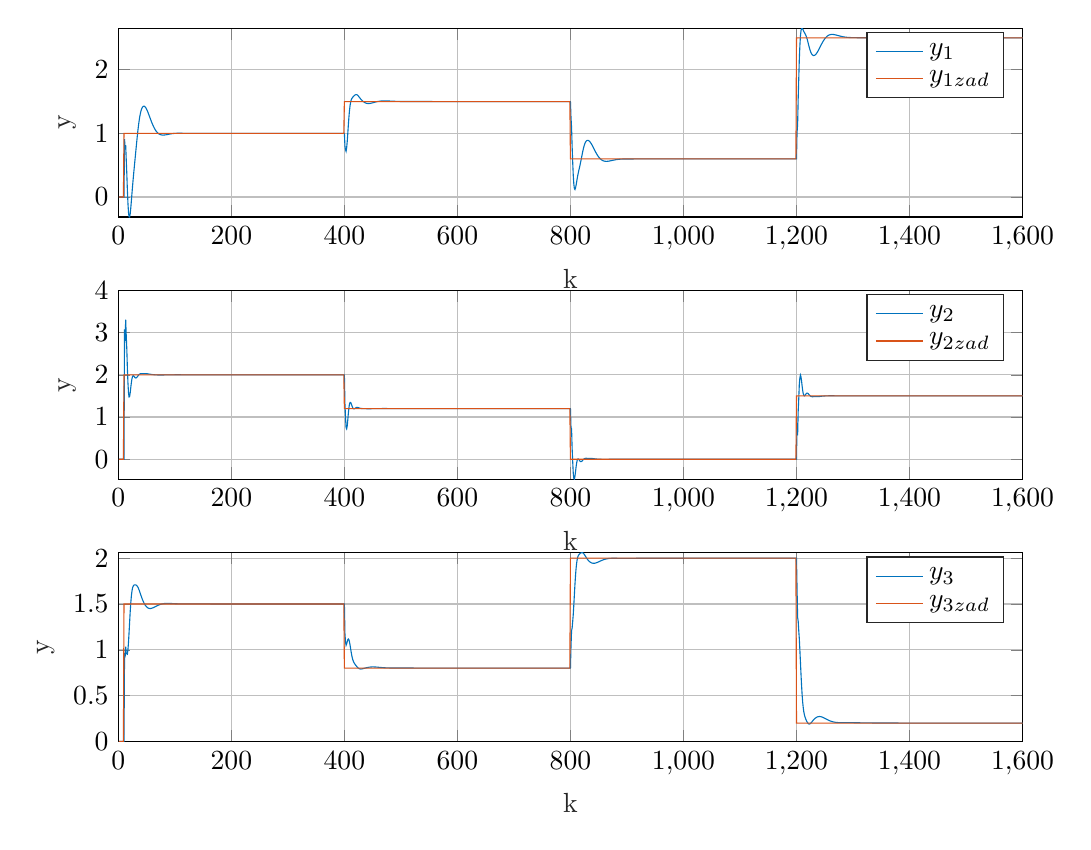
\begin{tikzpicture}

\begin{axis}[%
width=4.521in,
height=0.944in,
at={(0.758in,3.103in)},
scale only axis,
xmin=0,
xmax=1600,
xlabel style={font=\color{white!15!black}},
xlabel={k},
ymin=-0.3153,
ymax=2.6528,
ylabel style={font=\color{white!15!black}},
ylabel={y},
axis background/.style={fill=white},
xmajorgrids,
ymajorgrids,
legend style={legend cell align=left, align=left, draw=white!15!black}
]
\addplot [color=mycolor1]
  table[row sep=crcr]{%
1	0\\
2	0\\
3	0\\
4	0\\
5	0\\
6	0\\
7	0\\
8	0\\
9	0\\
10	0\\
11	0.91262\\
12	0.75093\\
13	0.81473\\
14	0.58421\\
15	0.36668\\
16	0.10856\\
17	-0.096623\\
18	-0.24329\\
19	-0.31292\\
20	-0.3153\\
21	-0.26329\\
22	-0.17584\\
23	-0.06956\\
24	0.042359\\
25	0.15199\\
26	0.2559\\
27	0.35411\\
28	0.44836\\
29	0.54082\\
30	0.63305\\
31	0.7255\\
32	0.81751\\
33	0.90755\\
34	0.99368\\
35	1.0739\\
36	1.1467\\
37	1.2109\\
38	1.2661\\
39	1.3121\\
40	1.3494\\
41	1.3786\\
42	1.4003\\
43	1.4153\\
44	1.4242\\
45	1.4276\\
46	1.426\\
47	1.4199\\
48	1.4098\\
49	1.3963\\
50	1.3797\\
51	1.3606\\
52	1.3396\\
53	1.3171\\
54	1.2936\\
55	1.2696\\
56	1.2454\\
57	1.2213\\
58	1.1978\\
59	1.1749\\
60	1.153\\
61	1.1321\\
62	1.1124\\
63	1.094\\
64	1.077\\
65	1.0614\\
66	1.0472\\
67	1.0344\\
68	1.0231\\
69	1.0131\\
70	1.0044\\
71	0.99702\\
72	0.99079\\
73	0.98566\\
74	0.98154\\
75	0.97835\\
76	0.976\\
77	0.9744\\
78	0.97345\\
79	0.97309\\
80	0.97322\\
81	0.97377\\
82	0.97467\\
83	0.97586\\
84	0.97725\\
85	0.97882\\
86	0.98049\\
87	0.98223\\
88	0.984\\
89	0.98576\\
90	0.98749\\
91	0.98916\\
92	0.99075\\
93	0.99224\\
94	0.99363\\
95	0.9949\\
96	0.99606\\
97	0.99709\\
98	0.99801\\
99	0.9988\\
100	0.99948\\
101	1\\
102	1.0005\\
103	1.0009\\
104	1.0012\\
105	1.0014\\
106	1.0015\\
107	1.0015\\
108	1.0015\\
109	1.0015\\
110	1.0014\\
111	1.0013\\
112	1.0012\\
113	1.001\\
114	1.0008\\
115	1.0006\\
116	1.0005\\
117	1.0003\\
118	1.0001\\
119	0.99992\\
120	0.99976\\
121	0.9996\\
122	0.99946\\
123	0.99934\\
124	0.99922\\
125	0.99912\\
126	0.99904\\
127	0.99897\\
128	0.99892\\
129	0.99888\\
130	0.99885\\
131	0.99883\\
132	0.99883\\
133	0.99883\\
134	0.99884\\
135	0.99887\\
136	0.9989\\
137	0.99893\\
138	0.99897\\
139	0.99901\\
140	0.99906\\
141	0.99911\\
142	0.99916\\
143	0.99921\\
144	0.99926\\
145	0.99931\\
146	0.99936\\
147	0.99941\\
148	0.99946\\
149	0.9995\\
150	0.99954\\
151	0.99959\\
152	0.99962\\
153	0.99966\\
154	0.99969\\
155	0.99972\\
156	0.99975\\
157	0.99977\\
158	0.99979\\
159	0.99982\\
160	0.99983\\
161	0.99985\\
162	0.99986\\
163	0.99988\\
164	0.99989\\
165	0.9999\\
166	0.9999\\
167	0.99991\\
168	0.99992\\
169	0.99992\\
170	0.99993\\
171	0.99993\\
172	0.99993\\
173	0.99993\\
174	0.99994\\
175	0.99994\\
176	0.99994\\
177	0.99994\\
178	0.99994\\
179	0.99994\\
180	0.99995\\
181	0.99995\\
182	0.99995\\
183	0.99995\\
184	0.99995\\
185	0.99995\\
186	0.99995\\
187	0.99995\\
188	0.99996\\
189	0.99996\\
190	0.99996\\
191	0.99996\\
192	0.99996\\
193	0.99996\\
194	0.99996\\
195	0.99997\\
196	0.99997\\
197	0.99997\\
198	0.99997\\
199	0.99997\\
200	0.99997\\
201	0.99998\\
202	0.99998\\
203	0.99998\\
204	0.99998\\
205	0.99998\\
206	0.99998\\
207	0.99998\\
208	0.99998\\
209	0.99999\\
210	0.99999\\
211	0.99999\\
212	0.99999\\
213	0.99999\\
214	0.99999\\
215	0.99999\\
216	0.99999\\
217	0.99999\\
218	0.99999\\
219	0.99999\\
220	0.99999\\
221	0.99999\\
222	0.99999\\
223	0.99999\\
224	0.99999\\
225	0.99999\\
226	1\\
227	1\\
228	1\\
229	1\\
230	1\\
231	1\\
232	1\\
233	1\\
234	1\\
235	1\\
236	1\\
237	1\\
238	1\\
239	1\\
240	1\\
241	1\\
242	1\\
243	1\\
244	1\\
245	1\\
246	1\\
247	1\\
248	1\\
249	1\\
250	1\\
251	1\\
252	1\\
253	1\\
254	1\\
255	1\\
256	1\\
257	1\\
258	1\\
259	1\\
260	1\\
261	1\\
262	1\\
263	1\\
264	1\\
265	1\\
266	1\\
267	1\\
268	1\\
269	1\\
270	1\\
271	1\\
272	1\\
273	1\\
274	1\\
275	1\\
276	1\\
277	1\\
278	1\\
279	1\\
280	1\\
281	1\\
282	1\\
283	1\\
284	1\\
285	1\\
286	1\\
287	1\\
288	1\\
289	1\\
290	1\\
291	1\\
292	1\\
293	1\\
294	1\\
295	1\\
296	1\\
297	1\\
298	1\\
299	1\\
300	1\\
301	1\\
302	1\\
303	1\\
304	1\\
305	1\\
306	1\\
307	1\\
308	1\\
309	1\\
310	1\\
311	1\\
312	1\\
313	1\\
314	1\\
315	1\\
316	1\\
317	1\\
318	1\\
319	1\\
320	1\\
321	1\\
322	1\\
323	1\\
324	1\\
325	1\\
326	1\\
327	1\\
328	1\\
329	1\\
330	1\\
331	1\\
332	1\\
333	1\\
334	1\\
335	1\\
336	1\\
337	1\\
338	1\\
339	1\\
340	1\\
341	1\\
342	1\\
343	1\\
344	1\\
345	1\\
346	1\\
347	1\\
348	1\\
349	1\\
350	1\\
351	1\\
352	1\\
353	1\\
354	1\\
355	1\\
356	1\\
357	1\\
358	1\\
359	1\\
360	1\\
361	1\\
362	1\\
363	1\\
364	1\\
365	1\\
366	1\\
367	1\\
368	1\\
369	1\\
370	1\\
371	1\\
372	1\\
373	1\\
374	1\\
375	1\\
376	1\\
377	1\\
378	1\\
379	1\\
380	1\\
381	1\\
382	1\\
383	1\\
384	1\\
385	1\\
386	1\\
387	1\\
388	1\\
389	1\\
390	1\\
391	1\\
392	1\\
393	1\\
394	1\\
395	1\\
396	1\\
397	1\\
398	1\\
399	1\\
400	1\\
401	0.79673\\
402	0.74089\\
403	0.71712\\
404	0.77179\\
405	0.86812\\
406	0.99543\\
407	1.1285\\
408	1.2522\\
409	1.355\\
410	1.4331\\
411	1.4876\\
412	1.5229\\
413	1.5449\\
414	1.5591\\
415	1.5698\\
416	1.5793\\
417	1.5884\\
418	1.597\\
419	1.604\\
420	1.6085\\
421	1.6098\\
422	1.6076\\
423	1.6021\\
424	1.5939\\
425	1.5838\\
426	1.5725\\
427	1.5609\\
428	1.5495\\
429	1.5385\\
430	1.5284\\
431	1.5191\\
432	1.5106\\
433	1.503\\
434	1.4961\\
435	1.49\\
436	1.4847\\
437	1.4802\\
438	1.4764\\
439	1.4735\\
440	1.4713\\
441	1.4699\\
442	1.4692\\
443	1.4691\\
444	1.4696\\
445	1.4706\\
446	1.4719\\
447	1.4737\\
448	1.4756\\
449	1.4778\\
450	1.4801\\
451	1.4825\\
452	1.485\\
453	1.4875\\
454	1.4899\\
455	1.4923\\
456	1.4946\\
457	1.4967\\
458	1.4988\\
459	1.5007\\
460	1.5024\\
461	1.504\\
462	1.5053\\
463	1.5066\\
464	1.5076\\
465	1.5085\\
466	1.5092\\
467	1.5098\\
468	1.5102\\
469	1.5105\\
470	1.5107\\
471	1.5107\\
472	1.5107\\
473	1.5106\\
474	1.5104\\
475	1.5101\\
476	1.5098\\
477	1.5094\\
478	1.509\\
479	1.5086\\
480	1.5081\\
481	1.5077\\
482	1.5072\\
483	1.5067\\
484	1.5063\\
485	1.5058\\
486	1.5054\\
487	1.5049\\
488	1.5045\\
489	1.5042\\
490	1.5038\\
491	1.5035\\
492	1.5031\\
493	1.5029\\
494	1.5026\\
495	1.5023\\
496	1.5021\\
497	1.5019\\
498	1.5018\\
499	1.5016\\
500	1.5015\\
501	1.5013\\
502	1.5012\\
503	1.5011\\
504	1.501\\
505	1.501\\
506	1.5009\\
507	1.5009\\
508	1.5008\\
509	1.5008\\
510	1.5007\\
511	1.5007\\
512	1.5007\\
513	1.5007\\
514	1.5006\\
515	1.5006\\
516	1.5006\\
517	1.5006\\
518	1.5006\\
519	1.5006\\
520	1.5005\\
521	1.5005\\
522	1.5005\\
523	1.5005\\
524	1.5005\\
525	1.5005\\
526	1.5004\\
527	1.5004\\
528	1.5004\\
529	1.5004\\
530	1.5004\\
531	1.5004\\
532	1.5003\\
533	1.5003\\
534	1.5003\\
535	1.5003\\
536	1.5003\\
537	1.5003\\
538	1.5002\\
539	1.5002\\
540	1.5002\\
541	1.5002\\
542	1.5002\\
543	1.5002\\
544	1.5001\\
545	1.5001\\
546	1.5001\\
547	1.5001\\
548	1.5001\\
549	1.5001\\
550	1.5001\\
551	1.5001\\
552	1.5001\\
553	1.5001\\
554	1.5001\\
555	1.5001\\
556	1.5\\
557	1.5\\
558	1.5\\
559	1.5\\
560	1.5\\
561	1.5\\
562	1.5\\
563	1.5\\
564	1.5\\
565	1.5\\
566	1.5\\
567	1.5\\
568	1.5\\
569	1.5\\
570	1.5\\
571	1.5\\
572	1.5\\
573	1.5\\
574	1.5\\
575	1.5\\
576	1.5\\
577	1.5\\
578	1.5\\
579	1.5\\
580	1.5\\
581	1.5\\
582	1.5\\
583	1.5\\
584	1.5\\
585	1.5\\
586	1.5\\
587	1.5\\
588	1.5\\
589	1.5\\
590	1.5\\
591	1.5\\
592	1.5\\
593	1.5\\
594	1.5\\
595	1.5\\
596	1.5\\
597	1.5\\
598	1.5\\
599	1.5\\
600	1.5\\
601	1.5\\
602	1.5\\
603	1.5\\
604	1.5\\
605	1.5\\
606	1.5\\
607	1.5\\
608	1.5\\
609	1.5\\
610	1.5\\
611	1.5\\
612	1.5\\
613	1.5\\
614	1.5\\
615	1.5\\
616	1.5\\
617	1.5\\
618	1.5\\
619	1.5\\
620	1.5\\
621	1.5\\
622	1.5\\
623	1.5\\
624	1.5\\
625	1.5\\
626	1.5\\
627	1.5\\
628	1.5\\
629	1.5\\
630	1.5\\
631	1.5\\
632	1.5\\
633	1.5\\
634	1.5\\
635	1.5\\
636	1.5\\
637	1.5\\
638	1.5\\
639	1.5\\
640	1.5\\
641	1.5\\
642	1.5\\
643	1.5\\
644	1.5\\
645	1.5\\
646	1.5\\
647	1.5\\
648	1.5\\
649	1.5\\
650	1.5\\
651	1.5\\
652	1.5\\
653	1.5\\
654	1.5\\
655	1.5\\
656	1.5\\
657	1.5\\
658	1.5\\
659	1.5\\
660	1.5\\
661	1.5\\
662	1.5\\
663	1.5\\
664	1.5\\
665	1.5\\
666	1.5\\
667	1.5\\
668	1.5\\
669	1.5\\
670	1.5\\
671	1.5\\
672	1.5\\
673	1.5\\
674	1.5\\
675	1.5\\
676	1.5\\
677	1.5\\
678	1.5\\
679	1.5\\
680	1.5\\
681	1.5\\
682	1.5\\
683	1.5\\
684	1.5\\
685	1.5\\
686	1.5\\
687	1.5\\
688	1.5\\
689	1.5\\
690	1.5\\
691	1.5\\
692	1.5\\
693	1.5\\
694	1.5\\
695	1.5\\
696	1.5\\
697	1.5\\
698	1.5\\
699	1.5\\
700	1.5\\
701	1.5\\
702	1.5\\
703	1.5\\
704	1.5\\
705	1.5\\
706	1.5\\
707	1.5\\
708	1.5\\
709	1.5\\
710	1.5\\
711	1.5\\
712	1.5\\
713	1.5\\
714	1.5\\
715	1.5\\
716	1.5\\
717	1.5\\
718	1.5\\
719	1.5\\
720	1.5\\
721	1.5\\
722	1.5\\
723	1.5\\
724	1.5\\
725	1.5\\
726	1.5\\
727	1.5\\
728	1.5\\
729	1.5\\
730	1.5\\
731	1.5\\
732	1.5\\
733	1.5\\
734	1.5\\
735	1.5\\
736	1.5\\
737	1.5\\
738	1.5\\
739	1.5\\
740	1.5\\
741	1.5\\
742	1.5\\
743	1.5\\
744	1.5\\
745	1.5\\
746	1.5\\
747	1.5\\
748	1.5\\
749	1.5\\
750	1.5\\
751	1.5\\
752	1.5\\
753	1.5\\
754	1.5\\
755	1.5\\
756	1.5\\
757	1.5\\
758	1.5\\
759	1.5\\
760	1.5\\
761	1.5\\
762	1.5\\
763	1.5\\
764	1.5\\
765	1.5\\
766	1.5\\
767	1.5\\
768	1.5\\
769	1.5\\
770	1.5\\
771	1.5\\
772	1.5\\
773	1.5\\
774	1.5\\
775	1.5\\
776	1.5\\
777	1.5\\
778	1.5\\
779	1.5\\
780	1.5\\
781	1.5\\
782	1.5\\
783	1.5\\
784	1.5\\
785	1.5\\
786	1.5\\
787	1.5\\
788	1.5\\
789	1.5\\
790	1.5\\
791	1.5\\
792	1.5\\
793	1.5\\
794	1.5\\
795	1.5\\
796	1.5\\
797	1.5\\
798	1.5\\
799	1.5\\
800	1.5\\
801	1.2477\\
802	1.0942\\
803	0.79188\\
804	0.55029\\
805	0.33958\\
806	0.2049\\
807	0.1328\\
808	0.11761\\
809	0.1403\\
810	0.18533\\
811	0.23867\\
812	0.29168\\
813	0.34006\\
814	0.38334\\
815	0.42319\\
816	0.46208\\
817	0.5021\\
818	0.54437\\
819	0.58887\\
820	0.63457\\
821	0.67989\\
822	0.72305\\
823	0.76247\\
824	0.79696\\
825	0.82587\\
826	0.84901\\
827	0.86656\\
828	0.87894\\
829	0.88671\\
830	0.89039\\
831	0.89049\\
832	0.88741\\
833	0.88151\\
834	0.87308\\
835	0.86242\\
836	0.84981\\
837	0.83555\\
838	0.81994\\
839	0.80333\\
840	0.78602\\
841	0.76834\\
842	0.75058\\
843	0.73298\\
844	0.71576\\
845	0.69911\\
846	0.68318\\
847	0.66808\\
848	0.65391\\
849	0.64072\\
850	0.62858\\
851	0.61749\\
852	0.60749\\
853	0.59856\\
854	0.59069\\
855	0.58385\\
856	0.57801\\
857	0.57311\\
858	0.56911\\
859	0.56594\\
860	0.56354\\
861	0.56183\\
862	0.56076\\
863	0.56025\\
864	0.56024\\
865	0.56066\\
866	0.56145\\
867	0.56255\\
868	0.5639\\
869	0.56546\\
870	0.56718\\
871	0.569\\
872	0.57091\\
873	0.57285\\
874	0.57479\\
875	0.57672\\
876	0.57861\\
877	0.58044\\
878	0.58219\\
879	0.58385\\
880	0.58542\\
881	0.58688\\
882	0.58823\\
883	0.58947\\
884	0.59061\\
885	0.59163\\
886	0.59255\\
887	0.59337\\
888	0.59409\\
889	0.59472\\
890	0.59527\\
891	0.59574\\
892	0.59614\\
893	0.59647\\
894	0.59675\\
895	0.59698\\
896	0.59716\\
897	0.59731\\
898	0.59742\\
899	0.5975\\
900	0.59756\\
901	0.59761\\
902	0.59764\\
903	0.59766\\
904	0.59768\\
905	0.59769\\
906	0.5977\\
907	0.59771\\
908	0.59772\\
909	0.59774\\
910	0.59776\\
911	0.59778\\
912	0.59781\\
913	0.59785\\
914	0.59789\\
915	0.59793\\
916	0.59799\\
917	0.59804\\
918	0.5981\\
919	0.59817\\
920	0.59824\\
921	0.59831\\
922	0.59838\\
923	0.59846\\
924	0.59853\\
925	0.59861\\
926	0.59869\\
927	0.59876\\
928	0.59884\\
929	0.59891\\
930	0.59898\\
931	0.59905\\
932	0.59911\\
933	0.59918\\
934	0.59924\\
935	0.5993\\
936	0.59935\\
937	0.5994\\
938	0.59945\\
939	0.5995\\
940	0.59954\\
941	0.59958\\
942	0.59962\\
943	0.59965\\
944	0.59968\\
945	0.59971\\
946	0.59973\\
947	0.59976\\
948	0.59978\\
949	0.5998\\
950	0.59981\\
951	0.59983\\
952	0.59984\\
953	0.59986\\
954	0.59987\\
955	0.59988\\
956	0.59989\\
957	0.59989\\
958	0.5999\\
959	0.59991\\
960	0.59991\\
961	0.59992\\
962	0.59992\\
963	0.59993\\
964	0.59993\\
965	0.59994\\
966	0.59994\\
967	0.59994\\
968	0.59995\\
969	0.59995\\
970	0.59995\\
971	0.59995\\
972	0.59996\\
973	0.59996\\
974	0.59996\\
975	0.59996\\
976	0.59997\\
977	0.59997\\
978	0.59997\\
979	0.59997\\
980	0.59997\\
981	0.59998\\
982	0.59998\\
983	0.59998\\
984	0.59998\\
985	0.59998\\
986	0.59999\\
987	0.59999\\
988	0.59999\\
989	0.59999\\
990	0.59999\\
991	0.59999\\
992	0.59999\\
993	0.59999\\
994	0.59999\\
995	0.6\\
996	0.6\\
997	0.6\\
998	0.6\\
999	0.6\\
1000	0.6\\
1001	0.6\\
1002	0.6\\
1003	0.6\\
1004	0.6\\
1005	0.6\\
1006	0.6\\
1007	0.6\\
1008	0.6\\
1009	0.6\\
1010	0.6\\
1011	0.6\\
1012	0.6\\
1013	0.6\\
1014	0.6\\
1015	0.6\\
1016	0.6\\
1017	0.6\\
1018	0.6\\
1019	0.6\\
1020	0.6\\
1021	0.6\\
1022	0.6\\
1023	0.6\\
1024	0.6\\
1025	0.6\\
1026	0.6\\
1027	0.6\\
1028	0.6\\
1029	0.6\\
1030	0.6\\
1031	0.6\\
1032	0.6\\
1033	0.6\\
1034	0.6\\
1035	0.6\\
1036	0.6\\
1037	0.6\\
1038	0.6\\
1039	0.6\\
1040	0.6\\
1041	0.6\\
1042	0.6\\
1043	0.6\\
1044	0.6\\
1045	0.6\\
1046	0.6\\
1047	0.6\\
1048	0.6\\
1049	0.6\\
1050	0.6\\
1051	0.6\\
1052	0.6\\
1053	0.6\\
1054	0.6\\
1055	0.6\\
1056	0.6\\
1057	0.6\\
1058	0.6\\
1059	0.6\\
1060	0.6\\
1061	0.6\\
1062	0.6\\
1063	0.6\\
1064	0.6\\
1065	0.6\\
1066	0.6\\
1067	0.6\\
1068	0.6\\
1069	0.6\\
1070	0.6\\
1071	0.6\\
1072	0.6\\
1073	0.6\\
1074	0.6\\
1075	0.6\\
1076	0.6\\
1077	0.6\\
1078	0.6\\
1079	0.6\\
1080	0.6\\
1081	0.6\\
1082	0.6\\
1083	0.6\\
1084	0.6\\
1085	0.6\\
1086	0.6\\
1087	0.6\\
1088	0.6\\
1089	0.6\\
1090	0.6\\
1091	0.6\\
1092	0.6\\
1093	0.6\\
1094	0.6\\
1095	0.6\\
1096	0.6\\
1097	0.6\\
1098	0.6\\
1099	0.6\\
1100	0.6\\
1101	0.6\\
1102	0.6\\
1103	0.6\\
1104	0.6\\
1105	0.6\\
1106	0.6\\
1107	0.6\\
1108	0.6\\
1109	0.6\\
1110	0.6\\
1111	0.6\\
1112	0.6\\
1113	0.6\\
1114	0.6\\
1115	0.6\\
1116	0.6\\
1117	0.6\\
1118	0.6\\
1119	0.6\\
1120	0.6\\
1121	0.6\\
1122	0.6\\
1123	0.6\\
1124	0.6\\
1125	0.6\\
1126	0.6\\
1127	0.6\\
1128	0.6\\
1129	0.6\\
1130	0.6\\
1131	0.6\\
1132	0.6\\
1133	0.6\\
1134	0.6\\
1135	0.6\\
1136	0.6\\
1137	0.6\\
1138	0.6\\
1139	0.6\\
1140	0.6\\
1141	0.6\\
1142	0.6\\
1143	0.6\\
1144	0.6\\
1145	0.6\\
1146	0.6\\
1147	0.6\\
1148	0.6\\
1149	0.6\\
1150	0.6\\
1151	0.6\\
1152	0.6\\
1153	0.6\\
1154	0.6\\
1155	0.6\\
1156	0.6\\
1157	0.6\\
1158	0.6\\
1159	0.6\\
1160	0.6\\
1161	0.6\\
1162	0.6\\
1163	0.6\\
1164	0.6\\
1165	0.6\\
1166	0.6\\
1167	0.6\\
1168	0.6\\
1169	0.6\\
1170	0.6\\
1171	0.6\\
1172	0.6\\
1173	0.6\\
1174	0.6\\
1175	0.6\\
1176	0.6\\
1177	0.6\\
1178	0.6\\
1179	0.6\\
1180	0.6\\
1181	0.6\\
1182	0.6\\
1183	0.6\\
1184	0.6\\
1185	0.6\\
1186	0.6\\
1187	0.6\\
1188	0.6\\
1189	0.6\\
1190	0.6\\
1191	0.6\\
1192	0.6\\
1193	0.6\\
1194	0.6\\
1195	0.6\\
1196	0.6\\
1197	0.6\\
1198	0.6\\
1199	0.6\\
1200	0.6\\
1201	1.0186\\
1202	1.1368\\
1203	1.5434\\
1204	1.8537\\
1205	2.1601\\
1206	2.3783\\
1207	2.5307\\
1208	2.6142\\
1209	2.6498\\
1210	2.6528\\
1211	2.6395\\
1212	2.6205\\
1213	2.6017\\
1214	2.585\\
1215	2.5692\\
1216	2.5524\\
1217	2.5321\\
1218	2.5073\\
1219	2.4777\\
1220	2.4443\\
1221	2.4089\\
1222	2.3734\\
1223	2.3397\\
1224	2.3093\\
1225	2.2834\\
1226	2.2623\\
1227	2.2462\\
1228	2.2348\\
1229	2.2276\\
1230	2.2242\\
1231	2.2243\\
1232	2.2273\\
1233	2.233\\
1234	2.2411\\
1235	2.2514\\
1236	2.2636\\
1237	2.2776\\
1238	2.2929\\
1239	2.3093\\
1240	2.3265\\
1241	2.3441\\
1242	2.3619\\
1243	2.3796\\
1244	2.397\\
1245	2.4139\\
1246	2.4301\\
1247	2.4455\\
1248	2.46\\
1249	2.4735\\
1250	2.486\\
1251	2.4974\\
1252	2.5076\\
1253	2.5168\\
1254	2.5249\\
1255	2.532\\
1256	2.5379\\
1257	2.5429\\
1258	2.547\\
1259	2.5502\\
1260	2.5525\\
1261	2.5541\\
1262	2.5551\\
1263	2.5554\\
1264	2.5552\\
1265	2.5545\\
1266	2.5534\\
1267	2.5519\\
1268	2.5502\\
1269	2.5482\\
1270	2.5461\\
1271	2.5438\\
1272	2.5414\\
1273	2.539\\
1274	2.5366\\
1275	2.5342\\
1276	2.5318\\
1277	2.5295\\
1278	2.5273\\
1279	2.5251\\
1280	2.5231\\
1281	2.5212\\
1282	2.5194\\
1283	2.5177\\
1284	2.5162\\
1285	2.5148\\
1286	2.5135\\
1287	2.5123\\
1288	2.5112\\
1289	2.5103\\
1290	2.5094\\
1291	2.5086\\
1292	2.508\\
1293	2.5074\\
1294	2.5068\\
1295	2.5064\\
1296	2.506\\
1297	2.5057\\
1298	2.5054\\
1299	2.5051\\
1300	2.5049\\
1301	2.5047\\
1302	2.5045\\
1303	2.5044\\
1304	2.5042\\
1305	2.5041\\
1306	2.504\\
1307	2.5039\\
1308	2.5038\\
1309	2.5037\\
1310	2.5036\\
1311	2.5035\\
1312	2.5034\\
1313	2.5033\\
1314	2.5032\\
1315	2.5031\\
1316	2.503\\
1317	2.5029\\
1318	2.5027\\
1319	2.5026\\
1320	2.5025\\
1321	2.5024\\
1322	2.5023\\
1323	2.5022\\
1324	2.5021\\
1325	2.502\\
1326	2.5019\\
1327	2.5017\\
1328	2.5016\\
1329	2.5015\\
1330	2.5014\\
1331	2.5013\\
1332	2.5013\\
1333	2.5012\\
1334	2.5011\\
1335	2.501\\
1336	2.5009\\
1337	2.5009\\
1338	2.5008\\
1339	2.5007\\
1340	2.5007\\
1341	2.5006\\
1342	2.5006\\
1343	2.5005\\
1344	2.5005\\
1345	2.5004\\
1346	2.5004\\
1347	2.5004\\
1348	2.5003\\
1349	2.5003\\
1350	2.5003\\
1351	2.5003\\
1352	2.5002\\
1353	2.5002\\
1354	2.5002\\
1355	2.5002\\
1356	2.5002\\
1357	2.5002\\
1358	2.5001\\
1359	2.5001\\
1360	2.5001\\
1361	2.5001\\
1362	2.5001\\
1363	2.5001\\
1364	2.5001\\
1365	2.5001\\
1366	2.5001\\
1367	2.5001\\
1368	2.5001\\
1369	2.5001\\
1370	2.5001\\
1371	2.5001\\
1372	2.5001\\
1373	2.5\\
1374	2.5\\
1375	2.5\\
1376	2.5\\
1377	2.5\\
1378	2.5\\
1379	2.5\\
1380	2.5\\
1381	2.5\\
1382	2.5\\
1383	2.5\\
1384	2.5\\
1385	2.5\\
1386	2.5\\
1387	2.5\\
1388	2.5\\
1389	2.5\\
1390	2.5\\
1391	2.5\\
1392	2.5\\
1393	2.5\\
1394	2.5\\
1395	2.5\\
1396	2.5\\
1397	2.5\\
1398	2.5\\
1399	2.5\\
1400	2.5\\
1401	2.5\\
1402	2.5\\
1403	2.5\\
1404	2.5\\
1405	2.5\\
1406	2.5\\
1407	2.5\\
1408	2.5\\
1409	2.5\\
1410	2.5\\
1411	2.5\\
1412	2.5\\
1413	2.5\\
1414	2.5\\
1415	2.5\\
1416	2.5\\
1417	2.5\\
1418	2.5\\
1419	2.5\\
1420	2.5\\
1421	2.5\\
1422	2.5\\
1423	2.5\\
1424	2.5\\
1425	2.5\\
1426	2.5\\
1427	2.5\\
1428	2.5\\
1429	2.5\\
1430	2.5\\
1431	2.5\\
1432	2.5\\
1433	2.5\\
1434	2.5\\
1435	2.5\\
1436	2.5\\
1437	2.5\\
1438	2.5\\
1439	2.5\\
1440	2.5\\
1441	2.5\\
1442	2.5\\
1443	2.5\\
1444	2.5\\
1445	2.5\\
1446	2.5\\
1447	2.5\\
1448	2.5\\
1449	2.5\\
1450	2.5\\
1451	2.5\\
1452	2.5\\
1453	2.5\\
1454	2.5\\
1455	2.5\\
1456	2.5\\
1457	2.5\\
1458	2.5\\
1459	2.5\\
1460	2.5\\
1461	2.5\\
1462	2.5\\
1463	2.5\\
1464	2.5\\
1465	2.5\\
1466	2.5\\
1467	2.5\\
1468	2.5\\
1469	2.5\\
1470	2.5\\
1471	2.5\\
1472	2.5\\
1473	2.5\\
1474	2.5\\
1475	2.5\\
1476	2.5\\
1477	2.5\\
1478	2.5\\
1479	2.5\\
1480	2.5\\
1481	2.5\\
1482	2.5\\
1483	2.5\\
1484	2.5\\
1485	2.5\\
1486	2.5\\
1487	2.5\\
1488	2.5\\
1489	2.5\\
1490	2.5\\
1491	2.5\\
1492	2.5\\
1493	2.5\\
1494	2.5\\
1495	2.5\\
1496	2.5\\
1497	2.5\\
1498	2.5\\
1499	2.5\\
1500	2.5\\
1501	2.5\\
1502	2.5\\
1503	2.5\\
1504	2.5\\
1505	2.5\\
1506	2.5\\
1507	2.5\\
1508	2.5\\
1509	2.5\\
1510	2.5\\
1511	2.5\\
1512	2.5\\
1513	2.5\\
1514	2.5\\
1515	2.5\\
1516	2.5\\
1517	2.5\\
1518	2.5\\
1519	2.5\\
1520	2.5\\
1521	2.5\\
1522	2.5\\
1523	2.5\\
1524	2.5\\
1525	2.5\\
1526	2.5\\
1527	2.5\\
1528	2.5\\
1529	2.5\\
1530	2.5\\
1531	2.5\\
1532	2.5\\
1533	2.5\\
1534	2.5\\
1535	2.5\\
1536	2.5\\
1537	2.5\\
1538	2.5\\
1539	2.5\\
1540	2.5\\
1541	2.5\\
1542	2.5\\
1543	2.5\\
1544	2.5\\
1545	2.5\\
1546	2.5\\
1547	2.5\\
1548	2.5\\
1549	2.5\\
1550	2.5\\
1551	2.5\\
1552	2.5\\
1553	2.5\\
1554	2.5\\
1555	2.5\\
1556	2.5\\
1557	2.5\\
1558	2.5\\
1559	2.5\\
1560	2.5\\
1561	2.5\\
1562	2.5\\
1563	2.5\\
1564	2.5\\
1565	2.5\\
1566	2.5\\
1567	2.5\\
1568	2.5\\
1569	2.5\\
1570	2.5\\
1571	2.5\\
1572	2.5\\
1573	2.5\\
1574	2.5\\
1575	2.5\\
1576	2.5\\
1577	2.5\\
1578	2.5\\
1579	2.5\\
1580	2.5\\
1581	2.5\\
1582	2.5\\
1583	2.5\\
1584	2.5\\
1585	2.5\\
1586	2.5\\
1587	2.5\\
1588	2.5\\
1589	2.5\\
1590	2.5\\
1591	2.5\\
1592	2.5\\
1593	2.5\\
1594	2.5\\
1595	2.5\\
1596	2.5\\
1597	2.5\\
1598	2.5\\
1599	2.5\\
1600	2.5\\
};
\addlegendentry{$\text{y}_\text{1}$}

\addplot [color=mycolor2]
  table[row sep=crcr]{%
1	0\\
2	0\\
3	0\\
4	0\\
5	0\\
6	0\\
7	0\\
8	0\\
9	0\\
10	1\\
11	1\\
12	1\\
13	1\\
14	1\\
15	1\\
16	1\\
17	1\\
18	1\\
19	1\\
20	1\\
21	1\\
22	1\\
23	1\\
24	1\\
25	1\\
26	1\\
27	1\\
28	1\\
29	1\\
30	1\\
31	1\\
32	1\\
33	1\\
34	1\\
35	1\\
36	1\\
37	1\\
38	1\\
39	1\\
40	1\\
41	1\\
42	1\\
43	1\\
44	1\\
45	1\\
46	1\\
47	1\\
48	1\\
49	1\\
50	1\\
51	1\\
52	1\\
53	1\\
54	1\\
55	1\\
56	1\\
57	1\\
58	1\\
59	1\\
60	1\\
61	1\\
62	1\\
63	1\\
64	1\\
65	1\\
66	1\\
67	1\\
68	1\\
69	1\\
70	1\\
71	1\\
72	1\\
73	1\\
74	1\\
75	1\\
76	1\\
77	1\\
78	1\\
79	1\\
80	1\\
81	1\\
82	1\\
83	1\\
84	1\\
85	1\\
86	1\\
87	1\\
88	1\\
89	1\\
90	1\\
91	1\\
92	1\\
93	1\\
94	1\\
95	1\\
96	1\\
97	1\\
98	1\\
99	1\\
100	1\\
101	1\\
102	1\\
103	1\\
104	1\\
105	1\\
106	1\\
107	1\\
108	1\\
109	1\\
110	1\\
111	1\\
112	1\\
113	1\\
114	1\\
115	1\\
116	1\\
117	1\\
118	1\\
119	1\\
120	1\\
121	1\\
122	1\\
123	1\\
124	1\\
125	1\\
126	1\\
127	1\\
128	1\\
129	1\\
130	1\\
131	1\\
132	1\\
133	1\\
134	1\\
135	1\\
136	1\\
137	1\\
138	1\\
139	1\\
140	1\\
141	1\\
142	1\\
143	1\\
144	1\\
145	1\\
146	1\\
147	1\\
148	1\\
149	1\\
150	1\\
151	1\\
152	1\\
153	1\\
154	1\\
155	1\\
156	1\\
157	1\\
158	1\\
159	1\\
160	1\\
161	1\\
162	1\\
163	1\\
164	1\\
165	1\\
166	1\\
167	1\\
168	1\\
169	1\\
170	1\\
171	1\\
172	1\\
173	1\\
174	1\\
175	1\\
176	1\\
177	1\\
178	1\\
179	1\\
180	1\\
181	1\\
182	1\\
183	1\\
184	1\\
185	1\\
186	1\\
187	1\\
188	1\\
189	1\\
190	1\\
191	1\\
192	1\\
193	1\\
194	1\\
195	1\\
196	1\\
197	1\\
198	1\\
199	1\\
200	1\\
201	1\\
202	1\\
203	1\\
204	1\\
205	1\\
206	1\\
207	1\\
208	1\\
209	1\\
210	1\\
211	1\\
212	1\\
213	1\\
214	1\\
215	1\\
216	1\\
217	1\\
218	1\\
219	1\\
220	1\\
221	1\\
222	1\\
223	1\\
224	1\\
225	1\\
226	1\\
227	1\\
228	1\\
229	1\\
230	1\\
231	1\\
232	1\\
233	1\\
234	1\\
235	1\\
236	1\\
237	1\\
238	1\\
239	1\\
240	1\\
241	1\\
242	1\\
243	1\\
244	1\\
245	1\\
246	1\\
247	1\\
248	1\\
249	1\\
250	1\\
251	1\\
252	1\\
253	1\\
254	1\\
255	1\\
256	1\\
257	1\\
258	1\\
259	1\\
260	1\\
261	1\\
262	1\\
263	1\\
264	1\\
265	1\\
266	1\\
267	1\\
268	1\\
269	1\\
270	1\\
271	1\\
272	1\\
273	1\\
274	1\\
275	1\\
276	1\\
277	1\\
278	1\\
279	1\\
280	1\\
281	1\\
282	1\\
283	1\\
284	1\\
285	1\\
286	1\\
287	1\\
288	1\\
289	1\\
290	1\\
291	1\\
292	1\\
293	1\\
294	1\\
295	1\\
296	1\\
297	1\\
298	1\\
299	1\\
300	1\\
301	1\\
302	1\\
303	1\\
304	1\\
305	1\\
306	1\\
307	1\\
308	1\\
309	1\\
310	1\\
311	1\\
312	1\\
313	1\\
314	1\\
315	1\\
316	1\\
317	1\\
318	1\\
319	1\\
320	1\\
321	1\\
322	1\\
323	1\\
324	1\\
325	1\\
326	1\\
327	1\\
328	1\\
329	1\\
330	1\\
331	1\\
332	1\\
333	1\\
334	1\\
335	1\\
336	1\\
337	1\\
338	1\\
339	1\\
340	1\\
341	1\\
342	1\\
343	1\\
344	1\\
345	1\\
346	1\\
347	1\\
348	1\\
349	1\\
350	1\\
351	1\\
352	1\\
353	1\\
354	1\\
355	1\\
356	1\\
357	1\\
358	1\\
359	1\\
360	1\\
361	1\\
362	1\\
363	1\\
364	1\\
365	1\\
366	1\\
367	1\\
368	1\\
369	1\\
370	1\\
371	1\\
372	1\\
373	1\\
374	1\\
375	1\\
376	1\\
377	1\\
378	1\\
379	1\\
380	1\\
381	1\\
382	1\\
383	1\\
384	1\\
385	1\\
386	1\\
387	1\\
388	1\\
389	1\\
390	1\\
391	1\\
392	1\\
393	1\\
394	1\\
395	1\\
396	1\\
397	1\\
398	1\\
399	1\\
400	1.5\\
401	1.5\\
402	1.5\\
403	1.5\\
404	1.5\\
405	1.5\\
406	1.5\\
407	1.5\\
408	1.5\\
409	1.5\\
410	1.5\\
411	1.5\\
412	1.5\\
413	1.5\\
414	1.5\\
415	1.5\\
416	1.5\\
417	1.5\\
418	1.5\\
419	1.5\\
420	1.5\\
421	1.5\\
422	1.5\\
423	1.5\\
424	1.5\\
425	1.5\\
426	1.5\\
427	1.5\\
428	1.5\\
429	1.5\\
430	1.5\\
431	1.5\\
432	1.5\\
433	1.5\\
434	1.5\\
435	1.5\\
436	1.5\\
437	1.5\\
438	1.5\\
439	1.5\\
440	1.5\\
441	1.5\\
442	1.5\\
443	1.5\\
444	1.5\\
445	1.5\\
446	1.5\\
447	1.5\\
448	1.5\\
449	1.5\\
450	1.5\\
451	1.5\\
452	1.5\\
453	1.5\\
454	1.5\\
455	1.5\\
456	1.5\\
457	1.5\\
458	1.5\\
459	1.5\\
460	1.5\\
461	1.5\\
462	1.5\\
463	1.5\\
464	1.5\\
465	1.5\\
466	1.5\\
467	1.5\\
468	1.5\\
469	1.5\\
470	1.5\\
471	1.5\\
472	1.5\\
473	1.5\\
474	1.5\\
475	1.5\\
476	1.5\\
477	1.5\\
478	1.5\\
479	1.5\\
480	1.5\\
481	1.5\\
482	1.5\\
483	1.5\\
484	1.5\\
485	1.5\\
486	1.5\\
487	1.5\\
488	1.5\\
489	1.5\\
490	1.5\\
491	1.5\\
492	1.5\\
493	1.5\\
494	1.5\\
495	1.5\\
496	1.5\\
497	1.5\\
498	1.5\\
499	1.5\\
500	1.5\\
501	1.5\\
502	1.5\\
503	1.5\\
504	1.5\\
505	1.5\\
506	1.5\\
507	1.5\\
508	1.5\\
509	1.5\\
510	1.5\\
511	1.5\\
512	1.5\\
513	1.5\\
514	1.5\\
515	1.5\\
516	1.5\\
517	1.5\\
518	1.5\\
519	1.5\\
520	1.5\\
521	1.5\\
522	1.5\\
523	1.5\\
524	1.5\\
525	1.5\\
526	1.5\\
527	1.5\\
528	1.5\\
529	1.5\\
530	1.5\\
531	1.5\\
532	1.5\\
533	1.5\\
534	1.5\\
535	1.5\\
536	1.5\\
537	1.5\\
538	1.5\\
539	1.5\\
540	1.5\\
541	1.5\\
542	1.5\\
543	1.5\\
544	1.5\\
545	1.5\\
546	1.5\\
547	1.5\\
548	1.5\\
549	1.5\\
550	1.5\\
551	1.5\\
552	1.5\\
553	1.5\\
554	1.5\\
555	1.5\\
556	1.5\\
557	1.5\\
558	1.5\\
559	1.5\\
560	1.5\\
561	1.5\\
562	1.5\\
563	1.5\\
564	1.5\\
565	1.5\\
566	1.5\\
567	1.5\\
568	1.5\\
569	1.5\\
570	1.5\\
571	1.5\\
572	1.5\\
573	1.5\\
574	1.5\\
575	1.5\\
576	1.5\\
577	1.5\\
578	1.5\\
579	1.5\\
580	1.5\\
581	1.5\\
582	1.5\\
583	1.5\\
584	1.5\\
585	1.5\\
586	1.5\\
587	1.5\\
588	1.5\\
589	1.5\\
590	1.5\\
591	1.5\\
592	1.5\\
593	1.5\\
594	1.5\\
595	1.5\\
596	1.5\\
597	1.5\\
598	1.5\\
599	1.5\\
600	1.5\\
601	1.5\\
602	1.5\\
603	1.5\\
604	1.5\\
605	1.5\\
606	1.5\\
607	1.5\\
608	1.5\\
609	1.5\\
610	1.5\\
611	1.5\\
612	1.5\\
613	1.5\\
614	1.5\\
615	1.5\\
616	1.5\\
617	1.5\\
618	1.5\\
619	1.5\\
620	1.5\\
621	1.5\\
622	1.5\\
623	1.5\\
624	1.5\\
625	1.5\\
626	1.5\\
627	1.5\\
628	1.5\\
629	1.5\\
630	1.5\\
631	1.5\\
632	1.5\\
633	1.5\\
634	1.5\\
635	1.5\\
636	1.5\\
637	1.5\\
638	1.5\\
639	1.5\\
640	1.5\\
641	1.5\\
642	1.5\\
643	1.5\\
644	1.5\\
645	1.5\\
646	1.5\\
647	1.5\\
648	1.5\\
649	1.5\\
650	1.5\\
651	1.5\\
652	1.5\\
653	1.5\\
654	1.5\\
655	1.5\\
656	1.5\\
657	1.5\\
658	1.5\\
659	1.5\\
660	1.5\\
661	1.5\\
662	1.5\\
663	1.5\\
664	1.5\\
665	1.5\\
666	1.5\\
667	1.5\\
668	1.5\\
669	1.5\\
670	1.5\\
671	1.5\\
672	1.5\\
673	1.5\\
674	1.5\\
675	1.5\\
676	1.5\\
677	1.5\\
678	1.5\\
679	1.5\\
680	1.5\\
681	1.5\\
682	1.5\\
683	1.5\\
684	1.5\\
685	1.5\\
686	1.5\\
687	1.5\\
688	1.5\\
689	1.5\\
690	1.5\\
691	1.5\\
692	1.5\\
693	1.5\\
694	1.5\\
695	1.5\\
696	1.5\\
697	1.5\\
698	1.5\\
699	1.5\\
700	1.5\\
701	1.5\\
702	1.5\\
703	1.5\\
704	1.5\\
705	1.5\\
706	1.5\\
707	1.5\\
708	1.5\\
709	1.5\\
710	1.5\\
711	1.5\\
712	1.5\\
713	1.5\\
714	1.5\\
715	1.5\\
716	1.5\\
717	1.5\\
718	1.5\\
719	1.5\\
720	1.5\\
721	1.5\\
722	1.5\\
723	1.5\\
724	1.5\\
725	1.5\\
726	1.5\\
727	1.5\\
728	1.5\\
729	1.5\\
730	1.5\\
731	1.5\\
732	1.5\\
733	1.5\\
734	1.5\\
735	1.5\\
736	1.5\\
737	1.5\\
738	1.5\\
739	1.5\\
740	1.5\\
741	1.5\\
742	1.5\\
743	1.5\\
744	1.5\\
745	1.5\\
746	1.5\\
747	1.5\\
748	1.5\\
749	1.5\\
750	1.5\\
751	1.5\\
752	1.5\\
753	1.5\\
754	1.5\\
755	1.5\\
756	1.5\\
757	1.5\\
758	1.5\\
759	1.5\\
760	1.5\\
761	1.5\\
762	1.5\\
763	1.5\\
764	1.5\\
765	1.5\\
766	1.5\\
767	1.5\\
768	1.5\\
769	1.5\\
770	1.5\\
771	1.5\\
772	1.5\\
773	1.5\\
774	1.5\\
775	1.5\\
776	1.5\\
777	1.5\\
778	1.5\\
779	1.5\\
780	1.5\\
781	1.5\\
782	1.5\\
783	1.5\\
784	1.5\\
785	1.5\\
786	1.5\\
787	1.5\\
788	1.5\\
789	1.5\\
790	1.5\\
791	1.5\\
792	1.5\\
793	1.5\\
794	1.5\\
795	1.5\\
796	1.5\\
797	1.5\\
798	1.5\\
799	1.5\\
800	0.6\\
801	0.6\\
802	0.6\\
803	0.6\\
804	0.6\\
805	0.6\\
806	0.6\\
807	0.6\\
808	0.6\\
809	0.6\\
810	0.6\\
811	0.6\\
812	0.6\\
813	0.6\\
814	0.6\\
815	0.6\\
816	0.6\\
817	0.6\\
818	0.6\\
819	0.6\\
820	0.6\\
821	0.6\\
822	0.6\\
823	0.6\\
824	0.6\\
825	0.6\\
826	0.6\\
827	0.6\\
828	0.6\\
829	0.6\\
830	0.6\\
831	0.6\\
832	0.6\\
833	0.6\\
834	0.6\\
835	0.6\\
836	0.6\\
837	0.6\\
838	0.6\\
839	0.6\\
840	0.6\\
841	0.6\\
842	0.6\\
843	0.6\\
844	0.6\\
845	0.6\\
846	0.6\\
847	0.6\\
848	0.6\\
849	0.6\\
850	0.6\\
851	0.6\\
852	0.6\\
853	0.6\\
854	0.6\\
855	0.6\\
856	0.6\\
857	0.6\\
858	0.6\\
859	0.6\\
860	0.6\\
861	0.6\\
862	0.6\\
863	0.6\\
864	0.6\\
865	0.6\\
866	0.6\\
867	0.6\\
868	0.6\\
869	0.6\\
870	0.6\\
871	0.6\\
872	0.6\\
873	0.6\\
874	0.6\\
875	0.6\\
876	0.6\\
877	0.6\\
878	0.6\\
879	0.6\\
880	0.6\\
881	0.6\\
882	0.6\\
883	0.6\\
884	0.6\\
885	0.6\\
886	0.6\\
887	0.6\\
888	0.6\\
889	0.6\\
890	0.6\\
891	0.6\\
892	0.6\\
893	0.6\\
894	0.6\\
895	0.6\\
896	0.6\\
897	0.6\\
898	0.6\\
899	0.6\\
900	0.6\\
901	0.6\\
902	0.6\\
903	0.6\\
904	0.6\\
905	0.6\\
906	0.6\\
907	0.6\\
908	0.6\\
909	0.6\\
910	0.6\\
911	0.6\\
912	0.6\\
913	0.6\\
914	0.6\\
915	0.6\\
916	0.6\\
917	0.6\\
918	0.6\\
919	0.6\\
920	0.6\\
921	0.6\\
922	0.6\\
923	0.6\\
924	0.6\\
925	0.6\\
926	0.6\\
927	0.6\\
928	0.6\\
929	0.6\\
930	0.6\\
931	0.6\\
932	0.6\\
933	0.6\\
934	0.6\\
935	0.6\\
936	0.6\\
937	0.6\\
938	0.6\\
939	0.6\\
940	0.6\\
941	0.6\\
942	0.6\\
943	0.6\\
944	0.6\\
945	0.6\\
946	0.6\\
947	0.6\\
948	0.6\\
949	0.6\\
950	0.6\\
951	0.6\\
952	0.6\\
953	0.6\\
954	0.6\\
955	0.6\\
956	0.6\\
957	0.6\\
958	0.6\\
959	0.6\\
960	0.6\\
961	0.6\\
962	0.6\\
963	0.6\\
964	0.6\\
965	0.6\\
966	0.6\\
967	0.6\\
968	0.6\\
969	0.6\\
970	0.6\\
971	0.6\\
972	0.6\\
973	0.6\\
974	0.6\\
975	0.6\\
976	0.6\\
977	0.6\\
978	0.6\\
979	0.6\\
980	0.6\\
981	0.6\\
982	0.6\\
983	0.6\\
984	0.6\\
985	0.6\\
986	0.6\\
987	0.6\\
988	0.6\\
989	0.6\\
990	0.6\\
991	0.6\\
992	0.6\\
993	0.6\\
994	0.6\\
995	0.6\\
996	0.6\\
997	0.6\\
998	0.6\\
999	0.6\\
1000	0.6\\
1001	0.6\\
1002	0.6\\
1003	0.6\\
1004	0.6\\
1005	0.6\\
1006	0.6\\
1007	0.6\\
1008	0.6\\
1009	0.6\\
1010	0.6\\
1011	0.6\\
1012	0.6\\
1013	0.6\\
1014	0.6\\
1015	0.6\\
1016	0.6\\
1017	0.6\\
1018	0.6\\
1019	0.6\\
1020	0.6\\
1021	0.6\\
1022	0.6\\
1023	0.6\\
1024	0.6\\
1025	0.6\\
1026	0.6\\
1027	0.6\\
1028	0.6\\
1029	0.6\\
1030	0.6\\
1031	0.6\\
1032	0.6\\
1033	0.6\\
1034	0.6\\
1035	0.6\\
1036	0.6\\
1037	0.6\\
1038	0.6\\
1039	0.6\\
1040	0.6\\
1041	0.6\\
1042	0.6\\
1043	0.6\\
1044	0.6\\
1045	0.6\\
1046	0.6\\
1047	0.6\\
1048	0.6\\
1049	0.6\\
1050	0.6\\
1051	0.6\\
1052	0.6\\
1053	0.6\\
1054	0.6\\
1055	0.6\\
1056	0.6\\
1057	0.6\\
1058	0.6\\
1059	0.6\\
1060	0.6\\
1061	0.6\\
1062	0.6\\
1063	0.6\\
1064	0.6\\
1065	0.6\\
1066	0.6\\
1067	0.6\\
1068	0.6\\
1069	0.6\\
1070	0.6\\
1071	0.6\\
1072	0.6\\
1073	0.6\\
1074	0.6\\
1075	0.6\\
1076	0.6\\
1077	0.6\\
1078	0.6\\
1079	0.6\\
1080	0.6\\
1081	0.6\\
1082	0.6\\
1083	0.6\\
1084	0.6\\
1085	0.6\\
1086	0.6\\
1087	0.6\\
1088	0.6\\
1089	0.6\\
1090	0.6\\
1091	0.6\\
1092	0.6\\
1093	0.6\\
1094	0.6\\
1095	0.6\\
1096	0.6\\
1097	0.6\\
1098	0.6\\
1099	0.6\\
1100	0.6\\
1101	0.6\\
1102	0.6\\
1103	0.6\\
1104	0.6\\
1105	0.6\\
1106	0.6\\
1107	0.6\\
1108	0.6\\
1109	0.6\\
1110	0.6\\
1111	0.6\\
1112	0.6\\
1113	0.6\\
1114	0.6\\
1115	0.6\\
1116	0.6\\
1117	0.6\\
1118	0.6\\
1119	0.6\\
1120	0.6\\
1121	0.6\\
1122	0.6\\
1123	0.6\\
1124	0.6\\
1125	0.6\\
1126	0.6\\
1127	0.6\\
1128	0.6\\
1129	0.6\\
1130	0.6\\
1131	0.6\\
1132	0.6\\
1133	0.6\\
1134	0.6\\
1135	0.6\\
1136	0.6\\
1137	0.6\\
1138	0.6\\
1139	0.6\\
1140	0.6\\
1141	0.6\\
1142	0.6\\
1143	0.6\\
1144	0.6\\
1145	0.6\\
1146	0.6\\
1147	0.6\\
1148	0.6\\
1149	0.6\\
1150	0.6\\
1151	0.6\\
1152	0.6\\
1153	0.6\\
1154	0.6\\
1155	0.6\\
1156	0.6\\
1157	0.6\\
1158	0.6\\
1159	0.6\\
1160	0.6\\
1161	0.6\\
1162	0.6\\
1163	0.6\\
1164	0.6\\
1165	0.6\\
1166	0.6\\
1167	0.6\\
1168	0.6\\
1169	0.6\\
1170	0.6\\
1171	0.6\\
1172	0.6\\
1173	0.6\\
1174	0.6\\
1175	0.6\\
1176	0.6\\
1177	0.6\\
1178	0.6\\
1179	0.6\\
1180	0.6\\
1181	0.6\\
1182	0.6\\
1183	0.6\\
1184	0.6\\
1185	0.6\\
1186	0.6\\
1187	0.6\\
1188	0.6\\
1189	0.6\\
1190	0.6\\
1191	0.6\\
1192	0.6\\
1193	0.6\\
1194	0.6\\
1195	0.6\\
1196	0.6\\
1197	0.6\\
1198	0.6\\
1199	0.6\\
1200	2.5\\
1201	2.5\\
1202	2.5\\
1203	2.5\\
1204	2.5\\
1205	2.5\\
1206	2.5\\
1207	2.5\\
1208	2.5\\
1209	2.5\\
1210	2.5\\
1211	2.5\\
1212	2.5\\
1213	2.5\\
1214	2.5\\
1215	2.5\\
1216	2.5\\
1217	2.5\\
1218	2.5\\
1219	2.5\\
1220	2.5\\
1221	2.5\\
1222	2.5\\
1223	2.5\\
1224	2.5\\
1225	2.5\\
1226	2.5\\
1227	2.5\\
1228	2.5\\
1229	2.5\\
1230	2.5\\
1231	2.5\\
1232	2.5\\
1233	2.5\\
1234	2.5\\
1235	2.5\\
1236	2.5\\
1237	2.5\\
1238	2.5\\
1239	2.5\\
1240	2.5\\
1241	2.5\\
1242	2.5\\
1243	2.5\\
1244	2.5\\
1245	2.5\\
1246	2.5\\
1247	2.5\\
1248	2.5\\
1249	2.5\\
1250	2.5\\
1251	2.5\\
1252	2.5\\
1253	2.5\\
1254	2.5\\
1255	2.5\\
1256	2.5\\
1257	2.5\\
1258	2.5\\
1259	2.5\\
1260	2.5\\
1261	2.5\\
1262	2.5\\
1263	2.5\\
1264	2.5\\
1265	2.5\\
1266	2.5\\
1267	2.5\\
1268	2.5\\
1269	2.5\\
1270	2.5\\
1271	2.5\\
1272	2.5\\
1273	2.5\\
1274	2.5\\
1275	2.5\\
1276	2.5\\
1277	2.5\\
1278	2.5\\
1279	2.5\\
1280	2.5\\
1281	2.5\\
1282	2.5\\
1283	2.5\\
1284	2.5\\
1285	2.5\\
1286	2.5\\
1287	2.5\\
1288	2.5\\
1289	2.5\\
1290	2.5\\
1291	2.5\\
1292	2.5\\
1293	2.5\\
1294	2.5\\
1295	2.5\\
1296	2.5\\
1297	2.5\\
1298	2.5\\
1299	2.5\\
1300	2.5\\
1301	2.5\\
1302	2.5\\
1303	2.5\\
1304	2.5\\
1305	2.5\\
1306	2.5\\
1307	2.5\\
1308	2.5\\
1309	2.5\\
1310	2.5\\
1311	2.5\\
1312	2.5\\
1313	2.5\\
1314	2.5\\
1315	2.5\\
1316	2.5\\
1317	2.5\\
1318	2.5\\
1319	2.5\\
1320	2.5\\
1321	2.5\\
1322	2.5\\
1323	2.5\\
1324	2.5\\
1325	2.5\\
1326	2.5\\
1327	2.5\\
1328	2.5\\
1329	2.5\\
1330	2.5\\
1331	2.5\\
1332	2.5\\
1333	2.5\\
1334	2.5\\
1335	2.5\\
1336	2.5\\
1337	2.5\\
1338	2.5\\
1339	2.5\\
1340	2.5\\
1341	2.5\\
1342	2.5\\
1343	2.5\\
1344	2.5\\
1345	2.5\\
1346	2.5\\
1347	2.5\\
1348	2.5\\
1349	2.5\\
1350	2.5\\
1351	2.5\\
1352	2.5\\
1353	2.5\\
1354	2.5\\
1355	2.5\\
1356	2.5\\
1357	2.5\\
1358	2.5\\
1359	2.5\\
1360	2.5\\
1361	2.5\\
1362	2.5\\
1363	2.5\\
1364	2.5\\
1365	2.5\\
1366	2.5\\
1367	2.5\\
1368	2.5\\
1369	2.5\\
1370	2.5\\
1371	2.5\\
1372	2.5\\
1373	2.5\\
1374	2.5\\
1375	2.5\\
1376	2.5\\
1377	2.5\\
1378	2.5\\
1379	2.5\\
1380	2.5\\
1381	2.5\\
1382	2.5\\
1383	2.5\\
1384	2.5\\
1385	2.5\\
1386	2.5\\
1387	2.5\\
1388	2.5\\
1389	2.5\\
1390	2.5\\
1391	2.5\\
1392	2.5\\
1393	2.5\\
1394	2.5\\
1395	2.5\\
1396	2.5\\
1397	2.5\\
1398	2.5\\
1399	2.5\\
1400	2.5\\
1401	2.5\\
1402	2.5\\
1403	2.5\\
1404	2.5\\
1405	2.5\\
1406	2.5\\
1407	2.5\\
1408	2.5\\
1409	2.5\\
1410	2.5\\
1411	2.5\\
1412	2.5\\
1413	2.5\\
1414	2.5\\
1415	2.5\\
1416	2.5\\
1417	2.5\\
1418	2.5\\
1419	2.5\\
1420	2.5\\
1421	2.5\\
1422	2.5\\
1423	2.5\\
1424	2.5\\
1425	2.5\\
1426	2.5\\
1427	2.5\\
1428	2.5\\
1429	2.5\\
1430	2.5\\
1431	2.5\\
1432	2.5\\
1433	2.5\\
1434	2.5\\
1435	2.5\\
1436	2.5\\
1437	2.5\\
1438	2.5\\
1439	2.5\\
1440	2.5\\
1441	2.5\\
1442	2.5\\
1443	2.5\\
1444	2.5\\
1445	2.5\\
1446	2.5\\
1447	2.5\\
1448	2.5\\
1449	2.5\\
1450	2.5\\
1451	2.5\\
1452	2.5\\
1453	2.5\\
1454	2.5\\
1455	2.5\\
1456	2.5\\
1457	2.5\\
1458	2.5\\
1459	2.5\\
1460	2.5\\
1461	2.5\\
1462	2.5\\
1463	2.5\\
1464	2.5\\
1465	2.5\\
1466	2.5\\
1467	2.5\\
1468	2.5\\
1469	2.5\\
1470	2.5\\
1471	2.5\\
1472	2.5\\
1473	2.5\\
1474	2.5\\
1475	2.5\\
1476	2.5\\
1477	2.5\\
1478	2.5\\
1479	2.5\\
1480	2.5\\
1481	2.5\\
1482	2.5\\
1483	2.5\\
1484	2.5\\
1485	2.5\\
1486	2.5\\
1487	2.5\\
1488	2.5\\
1489	2.5\\
1490	2.5\\
1491	2.5\\
1492	2.5\\
1493	2.5\\
1494	2.5\\
1495	2.5\\
1496	2.5\\
1497	2.5\\
1498	2.5\\
1499	2.5\\
1500	2.5\\
1501	2.5\\
1502	2.5\\
1503	2.5\\
1504	2.5\\
1505	2.5\\
1506	2.5\\
1507	2.5\\
1508	2.5\\
1509	2.5\\
1510	2.5\\
1511	2.5\\
1512	2.5\\
1513	2.5\\
1514	2.5\\
1515	2.5\\
1516	2.5\\
1517	2.5\\
1518	2.5\\
1519	2.5\\
1520	2.5\\
1521	2.5\\
1522	2.5\\
1523	2.5\\
1524	2.5\\
1525	2.5\\
1526	2.5\\
1527	2.5\\
1528	2.5\\
1529	2.5\\
1530	2.5\\
1531	2.5\\
1532	2.5\\
1533	2.5\\
1534	2.5\\
1535	2.5\\
1536	2.5\\
1537	2.5\\
1538	2.5\\
1539	2.5\\
1540	2.5\\
1541	2.5\\
1542	2.5\\
1543	2.5\\
1544	2.5\\
1545	2.5\\
1546	2.5\\
1547	2.5\\
1548	2.5\\
1549	2.5\\
1550	2.5\\
1551	2.5\\
1552	2.5\\
1553	2.5\\
1554	2.5\\
1555	2.5\\
1556	2.5\\
1557	2.5\\
1558	2.5\\
1559	2.5\\
1560	2.5\\
1561	2.5\\
1562	2.5\\
1563	2.5\\
1564	2.5\\
1565	2.5\\
1566	2.5\\
1567	2.5\\
1568	2.5\\
1569	2.5\\
1570	2.5\\
1571	2.5\\
1572	2.5\\
1573	2.5\\
1574	2.5\\
1575	2.5\\
1576	2.5\\
1577	2.5\\
1578	2.5\\
1579	2.5\\
1580	2.5\\
1581	2.5\\
1582	2.5\\
1583	2.5\\
1584	2.5\\
1585	2.5\\
1586	2.5\\
1587	2.5\\
1588	2.5\\
1589	2.5\\
1590	2.5\\
1591	2.5\\
1592	2.5\\
1593	2.5\\
1594	2.5\\
1595	2.5\\
1596	2.5\\
1597	2.5\\
1598	2.5\\
1599	2.5\\
1600	2.5\\
};
\addlegendentry{$\text{y}_{\text{1zad}}$}

\end{axis}

\begin{axis}[%
width=4.521in,
height=0.944in,
at={(0.758in,1.792in)},
scale only axis,
xmin=0,
xmax=1600,
xlabel style={font=\color{white!15!black}},
xlabel={k},
ymin=-0.47437,
ymax=4,
ylabel style={font=\color{white!15!black}},
ylabel={y},
axis background/.style={fill=white},
xmajorgrids,
ymajorgrids,
legend style={legend cell align=left, align=left, draw=white!15!black}
]
\addplot [color=mycolor1]
  table[row sep=crcr]{%
1	0\\
2	0\\
3	0\\
4	0\\
5	0\\
6	0\\
7	0\\
8	0\\
9	0\\
10	0\\
11	3.0764\\
12	2.8071\\
13	3.3049\\
14	2.9275\\
15	2.6131\\
16	2.1563\\
17	1.8136\\
18	1.573\\
19	1.4758\\
20	1.4873\\
21	1.5749\\
22	1.6937\\
23	1.8099\\
24	1.9004\\
25	1.956\\
26	1.9784\\
27	1.9761\\
28	1.9605\\
29	1.9424\\
30	1.9293\\
31	1.9252\\
32	1.9307\\
33	1.9438\\
34	1.9613\\
35	1.9799\\
36	1.9967\\
37	2.0102\\
38	2.0196\\
39	2.0254\\
40	2.0283\\
41	2.0292\\
42	2.0292\\
43	2.0289\\
44	2.0287\\
45	2.0287\\
46	2.0288\\
47	2.0288\\
48	2.0285\\
49	2.0279\\
50	2.0268\\
51	2.0252\\
52	2.0233\\
53	2.0211\\
54	2.0188\\
55	2.0165\\
56	2.0142\\
57	2.0121\\
58	2.0101\\
59	2.0082\\
60	2.0065\\
61	2.0049\\
62	2.0035\\
63	2.0021\\
64	2.0009\\
65	1.9999\\
66	1.9989\\
67	1.9981\\
68	1.9974\\
69	1.9969\\
70	1.9965\\
71	1.9961\\
72	1.9959\\
73	1.9958\\
74	1.9958\\
75	1.9958\\
76	1.9959\\
77	1.996\\
78	1.9962\\
79	1.9964\\
80	1.9966\\
81	1.9968\\
82	1.9971\\
83	1.9974\\
84	1.9976\\
85	1.9979\\
86	1.9982\\
87	1.9984\\
88	1.9987\\
89	1.9989\\
90	1.9991\\
91	1.9993\\
92	1.9995\\
93	1.9996\\
94	1.9998\\
95	1.9999\\
96	2\\
97	2.0001\\
98	2.0002\\
99	2.0002\\
100	2.0003\\
101	2.0003\\
102	2.0003\\
103	2.0003\\
104	2.0004\\
105	2.0004\\
106	2.0003\\
107	2.0003\\
108	2.0003\\
109	2.0003\\
110	2.0003\\
111	2.0002\\
112	2.0002\\
113	2.0002\\
114	2.0002\\
115	2.0001\\
116	2.0001\\
117	2.0001\\
118	2.0001\\
119	2\\
120	2\\
121	2\\
122	2\\
123	2\\
124	2\\
125	1.9999\\
126	1.9999\\
127	1.9999\\
128	1.9999\\
129	1.9999\\
130	1.9999\\
131	1.9999\\
132	1.9999\\
133	1.9999\\
134	1.9999\\
135	1.9999\\
136	1.9999\\
137	1.9999\\
138	1.9999\\
139	1.9999\\
140	1.9999\\
141	1.9999\\
142	1.9999\\
143	1.9999\\
144	2\\
145	2\\
146	2\\
147	2\\
148	2\\
149	2\\
150	2\\
151	2\\
152	2\\
153	2\\
154	2\\
155	2\\
156	2\\
157	2\\
158	2\\
159	2\\
160	2\\
161	2\\
162	2\\
163	2\\
164	2\\
165	2\\
166	2\\
167	2\\
168	2\\
169	2\\
170	2\\
171	2\\
172	2\\
173	2\\
174	2\\
175	2\\
176	2\\
177	2\\
178	2\\
179	2\\
180	2\\
181	2\\
182	2\\
183	2\\
184	2\\
185	2\\
186	2\\
187	2\\
188	2\\
189	2\\
190	2\\
191	2\\
192	2\\
193	2\\
194	2\\
195	2\\
196	2\\
197	2\\
198	2\\
199	2\\
200	2\\
201	2\\
202	2\\
203	2\\
204	2\\
205	2\\
206	2\\
207	2\\
208	2\\
209	2\\
210	2\\
211	2\\
212	2\\
213	2\\
214	2\\
215	2\\
216	2\\
217	2\\
218	2\\
219	2\\
220	2\\
221	2\\
222	2\\
223	2\\
224	2\\
225	2\\
226	2\\
227	2\\
228	2\\
229	2\\
230	2\\
231	2\\
232	2\\
233	2\\
234	2\\
235	2\\
236	2\\
237	2\\
238	2\\
239	2\\
240	2\\
241	2\\
242	2\\
243	2\\
244	2\\
245	2\\
246	2\\
247	2\\
248	2\\
249	2\\
250	2\\
251	2\\
252	2\\
253	2\\
254	2\\
255	2\\
256	2\\
257	2\\
258	2\\
259	2\\
260	2\\
261	2\\
262	2\\
263	2\\
264	2\\
265	2\\
266	2\\
267	2\\
268	2\\
269	2\\
270	2\\
271	2\\
272	2\\
273	2\\
274	2\\
275	2\\
276	2\\
277	2\\
278	2\\
279	2\\
280	2\\
281	2\\
282	2\\
283	2\\
284	2\\
285	2\\
286	2\\
287	2\\
288	2\\
289	2\\
290	2\\
291	2\\
292	2\\
293	2\\
294	2\\
295	2\\
296	2\\
297	2\\
298	2\\
299	2\\
300	2\\
301	2\\
302	2\\
303	2\\
304	2\\
305	2\\
306	2\\
307	2\\
308	2\\
309	2\\
310	2\\
311	2\\
312	2\\
313	2\\
314	2\\
315	2\\
316	2\\
317	2\\
318	2\\
319	2\\
320	2\\
321	2\\
322	2\\
323	2\\
324	2\\
325	2\\
326	2\\
327	2\\
328	2\\
329	2\\
330	2\\
331	2\\
332	2\\
333	2\\
334	2\\
335	2\\
336	2\\
337	2\\
338	2\\
339	2\\
340	2\\
341	2\\
342	2\\
343	2\\
344	2\\
345	2\\
346	2\\
347	2\\
348	2\\
349	2\\
350	2\\
351	2\\
352	2\\
353	2\\
354	2\\
355	2\\
356	2\\
357	2\\
358	2\\
359	2\\
360	2\\
361	2\\
362	2\\
363	2\\
364	2\\
365	2\\
366	2\\
367	2\\
368	2\\
369	2\\
370	2\\
371	2\\
372	2\\
373	2\\
374	2\\
375	2\\
376	2\\
377	2\\
378	2\\
379	2\\
380	2\\
381	2\\
382	2\\
383	2\\
384	2\\
385	2\\
386	2\\
387	2\\
388	2\\
389	2\\
390	2\\
391	2\\
392	2\\
393	2\\
394	2\\
395	2\\
396	2\\
397	2\\
398	2\\
399	2\\
400	2\\
401	1.3018\\
402	0.99049\\
403	0.74913\\
404	0.7189\\
405	0.78676\\
406	0.92964\\
407	1.0832\\
408	1.2159\\
409	1.3044\\
410	1.3452\\
411	1.3453\\
412	1.3186\\
413	1.2801\\
414	1.2424\\
415	1.2137\\
416	1.1975\\
417	1.1932\\
418	1.1976\\
419	1.2067\\
420	1.2164\\
421	1.2241\\
422	1.2283\\
423	1.2286\\
424	1.2258\\
425	1.2211\\
426	1.2158\\
427	1.2107\\
428	1.2065\\
429	1.2036\\
430	1.2018\\
431	1.2008\\
432	1.2004\\
433	1.2001\\
434	1.1999\\
435	1.1995\\
436	1.1989\\
437	1.1983\\
438	1.1976\\
439	1.197\\
440	1.1965\\
441	1.1962\\
442	1.196\\
443	1.196\\
444	1.1962\\
445	1.1963\\
446	1.1966\\
447	1.1968\\
448	1.1971\\
449	1.1974\\
450	1.1976\\
451	1.1979\\
452	1.1981\\
453	1.1983\\
454	1.1986\\
455	1.1988\\
456	1.1991\\
457	1.1993\\
458	1.1995\\
459	1.1997\\
460	1.1998\\
461	1.2\\
462	1.2001\\
463	1.2002\\
464	1.2003\\
465	1.2004\\
466	1.2004\\
467	1.2005\\
468	1.2005\\
469	1.2005\\
470	1.2005\\
471	1.2005\\
472	1.2005\\
473	1.2005\\
474	1.2005\\
475	1.2005\\
476	1.2004\\
477	1.2004\\
478	1.2004\\
479	1.2003\\
480	1.2003\\
481	1.2003\\
482	1.2002\\
483	1.2002\\
484	1.2002\\
485	1.2001\\
486	1.2001\\
487	1.2001\\
488	1.2\\
489	1.2\\
490	1.2\\
491	1.2\\
492	1.2\\
493	1.2\\
494	1.1999\\
495	1.1999\\
496	1.1999\\
497	1.1999\\
498	1.1999\\
499	1.1999\\
500	1.1999\\
501	1.1999\\
502	1.1999\\
503	1.1999\\
504	1.1999\\
505	1.1999\\
506	1.1999\\
507	1.1999\\
508	1.1999\\
509	1.1999\\
510	1.1999\\
511	1.1999\\
512	1.2\\
513	1.2\\
514	1.2\\
515	1.2\\
516	1.2\\
517	1.2\\
518	1.2\\
519	1.2\\
520	1.2\\
521	1.2\\
522	1.2\\
523	1.2\\
524	1.2\\
525	1.2\\
526	1.2\\
527	1.2\\
528	1.2\\
529	1.2\\
530	1.2\\
531	1.2\\
532	1.2\\
533	1.2\\
534	1.2\\
535	1.2\\
536	1.2\\
537	1.2\\
538	1.2\\
539	1.2\\
540	1.2\\
541	1.2\\
542	1.2\\
543	1.2\\
544	1.2\\
545	1.2\\
546	1.2\\
547	1.2\\
548	1.2\\
549	1.2\\
550	1.2\\
551	1.2\\
552	1.2\\
553	1.2\\
554	1.2\\
555	1.2\\
556	1.2\\
557	1.2\\
558	1.2\\
559	1.2\\
560	1.2\\
561	1.2\\
562	1.2\\
563	1.2\\
564	1.2\\
565	1.2\\
566	1.2\\
567	1.2\\
568	1.2\\
569	1.2\\
570	1.2\\
571	1.2\\
572	1.2\\
573	1.2\\
574	1.2\\
575	1.2\\
576	1.2\\
577	1.2\\
578	1.2\\
579	1.2\\
580	1.2\\
581	1.2\\
582	1.2\\
583	1.2\\
584	1.2\\
585	1.2\\
586	1.2\\
587	1.2\\
588	1.2\\
589	1.2\\
590	1.2\\
591	1.2\\
592	1.2\\
593	1.2\\
594	1.2\\
595	1.2\\
596	1.2\\
597	1.2\\
598	1.2\\
599	1.2\\
600	1.2\\
601	1.2\\
602	1.2\\
603	1.2\\
604	1.2\\
605	1.2\\
606	1.2\\
607	1.2\\
608	1.2\\
609	1.2\\
610	1.2\\
611	1.2\\
612	1.2\\
613	1.2\\
614	1.2\\
615	1.2\\
616	1.2\\
617	1.2\\
618	1.2\\
619	1.2\\
620	1.2\\
621	1.2\\
622	1.2\\
623	1.2\\
624	1.2\\
625	1.2\\
626	1.2\\
627	1.2\\
628	1.2\\
629	1.2\\
630	1.2\\
631	1.2\\
632	1.2\\
633	1.2\\
634	1.2\\
635	1.2\\
636	1.2\\
637	1.2\\
638	1.2\\
639	1.2\\
640	1.2\\
641	1.2\\
642	1.2\\
643	1.2\\
644	1.2\\
645	1.2\\
646	1.2\\
647	1.2\\
648	1.2\\
649	1.2\\
650	1.2\\
651	1.2\\
652	1.2\\
653	1.2\\
654	1.2\\
655	1.2\\
656	1.2\\
657	1.2\\
658	1.2\\
659	1.2\\
660	1.2\\
661	1.2\\
662	1.2\\
663	1.2\\
664	1.2\\
665	1.2\\
666	1.2\\
667	1.2\\
668	1.2\\
669	1.2\\
670	1.2\\
671	1.2\\
672	1.2\\
673	1.2\\
674	1.2\\
675	1.2\\
676	1.2\\
677	1.2\\
678	1.2\\
679	1.2\\
680	1.2\\
681	1.2\\
682	1.2\\
683	1.2\\
684	1.2\\
685	1.2\\
686	1.2\\
687	1.2\\
688	1.2\\
689	1.2\\
690	1.2\\
691	1.2\\
692	1.2\\
693	1.2\\
694	1.2\\
695	1.2\\
696	1.2\\
697	1.2\\
698	1.2\\
699	1.2\\
700	1.2\\
701	1.2\\
702	1.2\\
703	1.2\\
704	1.2\\
705	1.2\\
706	1.2\\
707	1.2\\
708	1.2\\
709	1.2\\
710	1.2\\
711	1.2\\
712	1.2\\
713	1.2\\
714	1.2\\
715	1.2\\
716	1.2\\
717	1.2\\
718	1.2\\
719	1.2\\
720	1.2\\
721	1.2\\
722	1.2\\
723	1.2\\
724	1.2\\
725	1.2\\
726	1.2\\
727	1.2\\
728	1.2\\
729	1.2\\
730	1.2\\
731	1.2\\
732	1.2\\
733	1.2\\
734	1.2\\
735	1.2\\
736	1.2\\
737	1.2\\
738	1.2\\
739	1.2\\
740	1.2\\
741	1.2\\
742	1.2\\
743	1.2\\
744	1.2\\
745	1.2\\
746	1.2\\
747	1.2\\
748	1.2\\
749	1.2\\
750	1.2\\
751	1.2\\
752	1.2\\
753	1.2\\
754	1.2\\
755	1.2\\
756	1.2\\
757	1.2\\
758	1.2\\
759	1.2\\
760	1.2\\
761	1.2\\
762	1.2\\
763	1.2\\
764	1.2\\
765	1.2\\
766	1.2\\
767	1.2\\
768	1.2\\
769	1.2\\
770	1.2\\
771	1.2\\
772	1.2\\
773	1.2\\
774	1.2\\
775	1.2\\
776	1.2\\
777	1.2\\
778	1.2\\
779	1.2\\
780	1.2\\
781	1.2\\
782	1.2\\
783	1.2\\
784	1.2\\
785	1.2\\
786	1.2\\
787	1.2\\
788	1.2\\
789	1.2\\
790	1.2\\
791	1.2\\
792	1.2\\
793	1.2\\
794	1.2\\
795	1.2\\
796	1.2\\
797	1.2\\
798	1.2\\
799	1.2\\
800	1.2\\
801	0.74699\\
802	0.72409\\
803	0.25361\\
804	-0.055169\\
805	-0.33107\\
806	-0.45401\\
807	-0.47437\\
808	-0.4066\\
809	-0.29869\\
810	-0.18348\\
811	-0.088247\\
812	-0.025205\\
813	0.0039553\\
814	0.0060049\\
815	-0.008569\\
816	-0.028942\\
817	-0.046598\\
818	-0.056465\\
819	-0.056977\\
820	-0.049295\\
821	-0.036184\\
822	-0.020884\\
823	-0.0062434\\
824	0.0057949\\
825	0.014332\\
826	0.019384\\
827	0.021589\\
828	0.021874\\
829	0.021166\\
830	0.020195\\
831	0.019411\\
832	0.018981\\
833	0.018859\\
834	0.018875\\
835	0.018823\\
836	0.018533\\
837	0.017901\\
838	0.016907\\
839	0.015594\\
840	0.014051\\
841	0.012382\\
842	0.010687\\
843	0.0090413\\
844	0.0074967\\
845	0.0060774\\
846	0.0047881\\
847	0.0036212\\
848	0.002564\\
849	0.0016044\\
850	0.00073431\\
851	-5.0132e-05\\
852	-0.00074886\\
853	-0.0013598\\
854	-0.0018808\\
855	-0.002311\\
856	-0.0026518\\
857	-0.0029073\\
858	-0.0030837\\
859	-0.0031888\\
860	-0.0032311\\
861	-0.0032195\\
862	-0.0031623\\
863	-0.0030671\\
864	-0.0029407\\
865	-0.0027893\\
866	-0.0026181\\
867	-0.0024319\\
868	-0.0022352\\
869	-0.0020321\\
870	-0.0018261\\
871	-0.0016208\\
872	-0.0014191\\
873	-0.0012237\\
874	-0.0010367\\
875	-0.00085982\\
876	-0.00069449\\
877	-0.00054165\\
878	-0.00040189\\
879	-0.00027552\\
880	-0.00016259\\
881	-6.2949e-05\\
882	2.3751e-05\\
883	9.7988e-05\\
884	0.00016036\\
885	0.00021155\\
886	0.00025233\\
887	0.00028352\\
888	0.00030596\\
889	0.00032054\\
890	0.00032812\\
891	0.00032958\\
892	0.00032576\\
893	0.00031746\\
894	0.00030547\\
895	0.00029048\\
896	0.00027318\\
897	0.00025416\\
898	0.00023397\\
899	0.00021311\\
900	0.000192\\
901	0.00017102\\
902	0.0001505\\
903	0.00013071\\
904	0.00011185\\
905	9.4117e-05\\
906	7.7629e-05\\
907	6.2485e-05\\
908	4.8742e-05\\
909	3.6428e-05\\
910	2.5544e-05\\
911	1.6067e-05\\
912	7.9547e-06\\
913	1.1484e-06\\
914	-4.4235e-06\\
915	-8.8429e-06\\
916	-1.2199e-05\\
917	-1.4585e-05\\
918	-1.61e-05\\
919	-1.6839e-05\\
920	-1.6901e-05\\
921	-1.6379e-05\\
922	-1.5366e-05\\
923	-1.3946e-05\\
924	-1.2203e-05\\
925	-1.0211e-05\\
926	-8.0394e-06\\
927	-5.7513e-06\\
928	-3.4029e-06\\
929	-1.0435e-06\\
930	1.2838e-06\\
931	3.5423e-06\\
932	5.7014e-06\\
933	7.736e-06\\
934	9.6267e-06\\
935	1.1359e-05\\
936	1.2922e-05\\
937	1.431e-05\\
938	1.552e-05\\
939	1.6554e-05\\
940	1.7414e-05\\
941	1.8106e-05\\
942	1.8637e-05\\
943	1.9017e-05\\
944	1.9256e-05\\
945	1.9366e-05\\
946	1.9356e-05\\
947	1.9241e-05\\
948	1.9032e-05\\
949	1.874e-05\\
950	1.8378e-05\\
951	1.7957e-05\\
952	1.7488e-05\\
953	1.698e-05\\
954	1.6443e-05\\
955	1.5886e-05\\
956	1.5316e-05\\
957	1.4741e-05\\
958	1.4166e-05\\
959	1.3598e-05\\
960	1.304e-05\\
961	1.2497e-05\\
962	1.1972e-05\\
963	1.1468e-05\\
964	1.0986e-05\\
965	1.0527e-05\\
966	1.0094e-05\\
967	9.6853e-06\\
968	9.3021e-06\\
969	8.9437e-06\\
970	8.6097e-06\\
971	8.2992e-06\\
972	8.0111e-06\\
973	7.7444e-06\\
974	7.4976e-06\\
975	7.2695e-06\\
976	7.0587e-06\\
977	6.8635e-06\\
978	6.6827e-06\\
979	6.5148e-06\\
980	6.3584e-06\\
981	6.2122e-06\\
982	6.075e-06\\
983	5.9456e-06\\
984	5.8229e-06\\
985	5.7059e-06\\
986	5.5937e-06\\
987	5.4855e-06\\
988	5.3807e-06\\
989	5.2785e-06\\
990	5.1784e-06\\
991	5.08e-06\\
992	4.9829e-06\\
993	4.8868e-06\\
994	4.7915e-06\\
995	4.6967e-06\\
996	4.6023e-06\\
997	4.5083e-06\\
998	4.4147e-06\\
999	4.3213e-06\\
1000	4.2283e-06\\
1001	4.1357e-06\\
1002	4.0436e-06\\
1003	3.952e-06\\
1004	3.861e-06\\
1005	3.7709e-06\\
1006	3.6816e-06\\
1007	3.5932e-06\\
1008	3.506e-06\\
1009	3.4199e-06\\
1010	3.3352e-06\\
1011	3.2518e-06\\
1012	3.1699e-06\\
1013	3.0895e-06\\
1014	3.0108e-06\\
1015	2.9337e-06\\
1016	2.8583e-06\\
1017	2.7846e-06\\
1018	2.7127e-06\\
1019	2.6426e-06\\
1020	2.5743e-06\\
1021	2.5078e-06\\
1022	2.443e-06\\
1023	2.38e-06\\
1024	2.3188e-06\\
1025	2.2593e-06\\
1026	2.2015e-06\\
1027	2.1453e-06\\
1028	2.0907e-06\\
1029	2.0377e-06\\
1030	1.9863e-06\\
1031	1.9363e-06\\
1032	1.8877e-06\\
1033	1.8405e-06\\
1034	1.7947e-06\\
1035	1.7501e-06\\
1036	1.7068e-06\\
1037	1.6647e-06\\
1038	1.6237e-06\\
1039	1.5839e-06\\
1040	1.5451e-06\\
1041	1.5073e-06\\
1042	1.4706e-06\\
1043	1.4347e-06\\
1044	1.3998e-06\\
1045	1.3658e-06\\
1046	1.3327e-06\\
1047	1.3003e-06\\
1048	1.2688e-06\\
1049	1.238e-06\\
1050	1.208e-06\\
1051	1.1787e-06\\
1052	1.1501e-06\\
1053	1.1222e-06\\
1054	1.0949e-06\\
1055	1.0683e-06\\
1056	1.0423e-06\\
1057	1.0169e-06\\
1058	9.9217e-07\\
1059	9.6799e-07\\
1060	9.4437e-07\\
1061	9.2131e-07\\
1062	8.988e-07\\
1063	8.7682e-07\\
1064	8.5537e-07\\
1065	8.3442e-07\\
1066	8.1397e-07\\
1067	7.9402e-07\\
1068	7.7454e-07\\
1069	7.5553e-07\\
1070	7.3698e-07\\
1071	7.1887e-07\\
1072	7.0121e-07\\
1073	6.8398e-07\\
1074	6.6717e-07\\
1075	6.5076e-07\\
1076	6.3476e-07\\
1077	6.1916e-07\\
1078	6.0394e-07\\
1079	5.8909e-07\\
1080	5.7461e-07\\
1081	5.6048e-07\\
1082	5.4671e-07\\
1083	5.3328e-07\\
1084	5.2018e-07\\
1085	5.074e-07\\
1086	4.9494e-07\\
1087	4.8279e-07\\
1088	4.7094e-07\\
1089	4.5939e-07\\
1090	4.4812e-07\\
1091	4.3713e-07\\
1092	4.2641e-07\\
1093	4.1596e-07\\
1094	4.0577e-07\\
1095	3.9583e-07\\
1096	3.8613e-07\\
1097	3.7667e-07\\
1098	3.6745e-07\\
1099	3.5845e-07\\
1100	3.4968e-07\\
1101	3.4112e-07\\
1102	3.3277e-07\\
1103	3.2462e-07\\
1104	3.1668e-07\\
1105	3.0893e-07\\
1106	3.0137e-07\\
1107	2.9399e-07\\
1108	2.868e-07\\
1109	2.7978e-07\\
1110	2.7294e-07\\
1111	2.6626e-07\\
1112	2.5974e-07\\
1113	2.5339e-07\\
1114	2.4719e-07\\
1115	2.4114e-07\\
1116	2.3524e-07\\
1117	2.2948e-07\\
1118	2.2386e-07\\
1119	2.1839e-07\\
1120	2.1304e-07\\
1121	2.0783e-07\\
1122	2.0274e-07\\
1123	1.9778e-07\\
1124	1.9293e-07\\
1125	1.8821e-07\\
1126	1.836e-07\\
1127	1.7911e-07\\
1128	1.7472e-07\\
1129	1.7045e-07\\
1130	1.6627e-07\\
1131	1.622e-07\\
1132	1.5823e-07\\
1133	1.5436e-07\\
1134	1.5058e-07\\
1135	1.4689e-07\\
1136	1.433e-07\\
1137	1.3979e-07\\
1138	1.3637e-07\\
1139	1.3303e-07\\
1140	1.2977e-07\\
1141	1.2659e-07\\
1142	1.2349e-07\\
1143	1.2047e-07\\
1144	1.1752e-07\\
1145	1.1465e-07\\
1146	1.1184e-07\\
1147	1.091e-07\\
1148	1.0643e-07\\
1149	1.0382e-07\\
1150	1.0128e-07\\
1151	9.8804e-08\\
1152	9.6386e-08\\
1153	9.4027e-08\\
1154	9.1725e-08\\
1155	8.948e-08\\
1156	8.729e-08\\
1157	8.5154e-08\\
1158	8.3069e-08\\
1159	8.1036e-08\\
1160	7.9053e-08\\
1161	7.7118e-08\\
1162	7.5231e-08\\
1163	7.3389e-08\\
1164	7.1593e-08\\
1165	6.9841e-08\\
1166	6.8132e-08\\
1167	6.6464e-08\\
1168	6.4838e-08\\
1169	6.3251e-08\\
1170	6.1703e-08\\
1171	6.0193e-08\\
1172	5.8719e-08\\
1173	5.7282e-08\\
1174	5.588e-08\\
1175	5.4513e-08\\
1176	5.3178e-08\\
1177	5.1877e-08\\
1178	5.0607e-08\\
1179	4.9369e-08\\
1180	4.816e-08\\
1181	4.6982e-08\\
1182	4.5832e-08\\
1183	4.471e-08\\
1184	4.3616e-08\\
1185	4.2548e-08\\
1186	4.1507e-08\\
1187	4.0491e-08\\
1188	3.95e-08\\
1189	3.8533e-08\\
1190	3.759e-08\\
1191	3.667e-08\\
1192	3.5772e-08\\
1193	3.4897e-08\\
1194	3.4043e-08\\
1195	3.321e-08\\
1196	3.2397e-08\\
1197	3.1604e-08\\
1198	3.083e-08\\
1199	3.0076e-08\\
1200	2.934e-08\\
1201	0.86219\\
1202	0.5635\\
1203	1.1345\\
1204	1.4261\\
1205	1.7712\\
1206	1.933\\
1207	1.9955\\
1208	1.9488\\
1209	1.8498\\
1210	1.7307\\
1211	1.6254\\
1212	1.5499\\
1213	1.5098\\
1214	1.5001\\
1215	1.5111\\
1216	1.5313\\
1217	1.551\\
1218	1.5639\\
1219	1.5671\\
1220	1.5613\\
1221	1.5488\\
1222	1.533\\
1223	1.517\\
1224	1.5031\\
1225	1.4927\\
1226	1.4859\\
1227	1.4823\\
1228	1.4811\\
1229	1.4811\\
1230	1.4817\\
1231	1.4822\\
1232	1.4825\\
1233	1.4823\\
1234	1.4821\\
1235	1.4818\\
1236	1.4818\\
1237	1.4821\\
1238	1.4828\\
1239	1.4839\\
1240	1.4853\\
1241	1.4869\\
1242	1.4885\\
1243	1.4902\\
1244	1.4917\\
1245	1.4932\\
1246	1.4945\\
1247	1.4957\\
1248	1.4968\\
1249	1.4979\\
1250	1.4988\\
1251	1.4996\\
1252	1.5004\\
1253	1.5011\\
1254	1.5016\\
1255	1.5021\\
1256	1.5025\\
1257	1.5028\\
1258	1.5031\\
1259	1.5032\\
1260	1.5033\\
1261	1.5033\\
1262	1.5033\\
1263	1.5032\\
1264	1.5031\\
1265	1.503\\
1266	1.5028\\
1267	1.5026\\
1268	1.5024\\
1269	1.5022\\
1270	1.502\\
1271	1.5018\\
1272	1.5016\\
1273	1.5014\\
1274	1.5012\\
1275	1.501\\
1276	1.5008\\
1277	1.5006\\
1278	1.5005\\
1279	1.5003\\
1280	1.5002\\
1281	1.5001\\
1282	1.5\\
1283	1.4999\\
1284	1.4998\\
1285	1.4998\\
1286	1.4997\\
1287	1.4997\\
1288	1.4997\\
1289	1.4996\\
1290	1.4996\\
1291	1.4996\\
1292	1.4996\\
1293	1.4996\\
1294	1.4996\\
1295	1.4996\\
1296	1.4997\\
1297	1.4997\\
1298	1.4997\\
1299	1.4997\\
1300	1.4997\\
1301	1.4998\\
1302	1.4998\\
1303	1.4998\\
1304	1.4998\\
1305	1.4998\\
1306	1.4999\\
1307	1.4999\\
1308	1.4999\\
1309	1.4999\\
1310	1.4999\\
1311	1.4999\\
1312	1.4999\\
1313	1.5\\
1314	1.5\\
1315	1.5\\
1316	1.5\\
1317	1.5\\
1318	1.5\\
1319	1.5\\
1320	1.5\\
1321	1.5\\
1322	1.5\\
1323	1.5\\
1324	1.5\\
1325	1.5\\
1326	1.5\\
1327	1.5\\
1328	1.5\\
1329	1.5\\
1330	1.5\\
1331	1.5\\
1332	1.5\\
1333	1.5\\
1334	1.5\\
1335	1.5\\
1336	1.5\\
1337	1.5\\
1338	1.5\\
1339	1.5\\
1340	1.5\\
1341	1.5\\
1342	1.5\\
1343	1.5\\
1344	1.5\\
1345	1.5\\
1346	1.5\\
1347	1.5\\
1348	1.5\\
1349	1.5\\
1350	1.5\\
1351	1.5\\
1352	1.5\\
1353	1.5\\
1354	1.5\\
1355	1.5\\
1356	1.5\\
1357	1.5\\
1358	1.5\\
1359	1.5\\
1360	1.5\\
1361	1.5\\
1362	1.5\\
1363	1.5\\
1364	1.5\\
1365	1.5\\
1366	1.5\\
1367	1.5\\
1368	1.5\\
1369	1.5\\
1370	1.5\\
1371	1.5\\
1372	1.5\\
1373	1.5\\
1374	1.5\\
1375	1.5\\
1376	1.5\\
1377	1.5\\
1378	1.5\\
1379	1.5\\
1380	1.5\\
1381	1.5\\
1382	1.5\\
1383	1.5\\
1384	1.5\\
1385	1.5\\
1386	1.5\\
1387	1.5\\
1388	1.5\\
1389	1.5\\
1390	1.5\\
1391	1.5\\
1392	1.5\\
1393	1.5\\
1394	1.5\\
1395	1.5\\
1396	1.5\\
1397	1.5\\
1398	1.5\\
1399	1.5\\
1400	1.5\\
1401	1.5\\
1402	1.5\\
1403	1.5\\
1404	1.5\\
1405	1.5\\
1406	1.5\\
1407	1.5\\
1408	1.5\\
1409	1.5\\
1410	1.5\\
1411	1.5\\
1412	1.5\\
1413	1.5\\
1414	1.5\\
1415	1.5\\
1416	1.5\\
1417	1.5\\
1418	1.5\\
1419	1.5\\
1420	1.5\\
1421	1.5\\
1422	1.5\\
1423	1.5\\
1424	1.5\\
1425	1.5\\
1426	1.5\\
1427	1.5\\
1428	1.5\\
1429	1.5\\
1430	1.5\\
1431	1.5\\
1432	1.5\\
1433	1.5\\
1434	1.5\\
1435	1.5\\
1436	1.5\\
1437	1.5\\
1438	1.5\\
1439	1.5\\
1440	1.5\\
1441	1.5\\
1442	1.5\\
1443	1.5\\
1444	1.5\\
1445	1.5\\
1446	1.5\\
1447	1.5\\
1448	1.5\\
1449	1.5\\
1450	1.5\\
1451	1.5\\
1452	1.5\\
1453	1.5\\
1454	1.5\\
1455	1.5\\
1456	1.5\\
1457	1.5\\
1458	1.5\\
1459	1.5\\
1460	1.5\\
1461	1.5\\
1462	1.5\\
1463	1.5\\
1464	1.5\\
1465	1.5\\
1466	1.5\\
1467	1.5\\
1468	1.5\\
1469	1.5\\
1470	1.5\\
1471	1.5\\
1472	1.5\\
1473	1.5\\
1474	1.5\\
1475	1.5\\
1476	1.5\\
1477	1.5\\
1478	1.5\\
1479	1.5\\
1480	1.5\\
1481	1.5\\
1482	1.5\\
1483	1.5\\
1484	1.5\\
1485	1.5\\
1486	1.5\\
1487	1.5\\
1488	1.5\\
1489	1.5\\
1490	1.5\\
1491	1.5\\
1492	1.5\\
1493	1.5\\
1494	1.5\\
1495	1.5\\
1496	1.5\\
1497	1.5\\
1498	1.5\\
1499	1.5\\
1500	1.5\\
1501	1.5\\
1502	1.5\\
1503	1.5\\
1504	1.5\\
1505	1.5\\
1506	1.5\\
1507	1.5\\
1508	1.5\\
1509	1.5\\
1510	1.5\\
1511	1.5\\
1512	1.5\\
1513	1.5\\
1514	1.5\\
1515	1.5\\
1516	1.5\\
1517	1.5\\
1518	1.5\\
1519	1.5\\
1520	1.5\\
1521	1.5\\
1522	1.5\\
1523	1.5\\
1524	1.5\\
1525	1.5\\
1526	1.5\\
1527	1.5\\
1528	1.5\\
1529	1.5\\
1530	1.5\\
1531	1.5\\
1532	1.5\\
1533	1.5\\
1534	1.5\\
1535	1.5\\
1536	1.5\\
1537	1.5\\
1538	1.5\\
1539	1.5\\
1540	1.5\\
1541	1.5\\
1542	1.5\\
1543	1.5\\
1544	1.5\\
1545	1.5\\
1546	1.5\\
1547	1.5\\
1548	1.5\\
1549	1.5\\
1550	1.5\\
1551	1.5\\
1552	1.5\\
1553	1.5\\
1554	1.5\\
1555	1.5\\
1556	1.5\\
1557	1.5\\
1558	1.5\\
1559	1.5\\
1560	1.5\\
1561	1.5\\
1562	1.5\\
1563	1.5\\
1564	1.5\\
1565	1.5\\
1566	1.5\\
1567	1.5\\
1568	1.5\\
1569	1.5\\
1570	1.5\\
1571	1.5\\
1572	1.5\\
1573	1.5\\
1574	1.5\\
1575	1.5\\
1576	1.5\\
1577	1.5\\
1578	1.5\\
1579	1.5\\
1580	1.5\\
1581	1.5\\
1582	1.5\\
1583	1.5\\
1584	1.5\\
1585	1.5\\
1586	1.5\\
1587	1.5\\
1588	1.5\\
1589	1.5\\
1590	1.5\\
1591	1.5\\
1592	1.5\\
1593	1.5\\
1594	1.5\\
1595	1.5\\
1596	1.5\\
1597	1.5\\
1598	1.5\\
1599	1.5\\
1600	1.5\\
};
\addlegendentry{$\text{y}_\text{2}$}

\addplot [color=mycolor2]
  table[row sep=crcr]{%
1	0\\
2	0\\
3	0\\
4	0\\
5	0\\
6	0\\
7	0\\
8	0\\
9	0\\
10	2\\
11	2\\
12	2\\
13	2\\
14	2\\
15	2\\
16	2\\
17	2\\
18	2\\
19	2\\
20	2\\
21	2\\
22	2\\
23	2\\
24	2\\
25	2\\
26	2\\
27	2\\
28	2\\
29	2\\
30	2\\
31	2\\
32	2\\
33	2\\
34	2\\
35	2\\
36	2\\
37	2\\
38	2\\
39	2\\
40	2\\
41	2\\
42	2\\
43	2\\
44	2\\
45	2\\
46	2\\
47	2\\
48	2\\
49	2\\
50	2\\
51	2\\
52	2\\
53	2\\
54	2\\
55	2\\
56	2\\
57	2\\
58	2\\
59	2\\
60	2\\
61	2\\
62	2\\
63	2\\
64	2\\
65	2\\
66	2\\
67	2\\
68	2\\
69	2\\
70	2\\
71	2\\
72	2\\
73	2\\
74	2\\
75	2\\
76	2\\
77	2\\
78	2\\
79	2\\
80	2\\
81	2\\
82	2\\
83	2\\
84	2\\
85	2\\
86	2\\
87	2\\
88	2\\
89	2\\
90	2\\
91	2\\
92	2\\
93	2\\
94	2\\
95	2\\
96	2\\
97	2\\
98	2\\
99	2\\
100	2\\
101	2\\
102	2\\
103	2\\
104	2\\
105	2\\
106	2\\
107	2\\
108	2\\
109	2\\
110	2\\
111	2\\
112	2\\
113	2\\
114	2\\
115	2\\
116	2\\
117	2\\
118	2\\
119	2\\
120	2\\
121	2\\
122	2\\
123	2\\
124	2\\
125	2\\
126	2\\
127	2\\
128	2\\
129	2\\
130	2\\
131	2\\
132	2\\
133	2\\
134	2\\
135	2\\
136	2\\
137	2\\
138	2\\
139	2\\
140	2\\
141	2\\
142	2\\
143	2\\
144	2\\
145	2\\
146	2\\
147	2\\
148	2\\
149	2\\
150	2\\
151	2\\
152	2\\
153	2\\
154	2\\
155	2\\
156	2\\
157	2\\
158	2\\
159	2\\
160	2\\
161	2\\
162	2\\
163	2\\
164	2\\
165	2\\
166	2\\
167	2\\
168	2\\
169	2\\
170	2\\
171	2\\
172	2\\
173	2\\
174	2\\
175	2\\
176	2\\
177	2\\
178	2\\
179	2\\
180	2\\
181	2\\
182	2\\
183	2\\
184	2\\
185	2\\
186	2\\
187	2\\
188	2\\
189	2\\
190	2\\
191	2\\
192	2\\
193	2\\
194	2\\
195	2\\
196	2\\
197	2\\
198	2\\
199	2\\
200	2\\
201	2\\
202	2\\
203	2\\
204	2\\
205	2\\
206	2\\
207	2\\
208	2\\
209	2\\
210	2\\
211	2\\
212	2\\
213	2\\
214	2\\
215	2\\
216	2\\
217	2\\
218	2\\
219	2\\
220	2\\
221	2\\
222	2\\
223	2\\
224	2\\
225	2\\
226	2\\
227	2\\
228	2\\
229	2\\
230	2\\
231	2\\
232	2\\
233	2\\
234	2\\
235	2\\
236	2\\
237	2\\
238	2\\
239	2\\
240	2\\
241	2\\
242	2\\
243	2\\
244	2\\
245	2\\
246	2\\
247	2\\
248	2\\
249	2\\
250	2\\
251	2\\
252	2\\
253	2\\
254	2\\
255	2\\
256	2\\
257	2\\
258	2\\
259	2\\
260	2\\
261	2\\
262	2\\
263	2\\
264	2\\
265	2\\
266	2\\
267	2\\
268	2\\
269	2\\
270	2\\
271	2\\
272	2\\
273	2\\
274	2\\
275	2\\
276	2\\
277	2\\
278	2\\
279	2\\
280	2\\
281	2\\
282	2\\
283	2\\
284	2\\
285	2\\
286	2\\
287	2\\
288	2\\
289	2\\
290	2\\
291	2\\
292	2\\
293	2\\
294	2\\
295	2\\
296	2\\
297	2\\
298	2\\
299	2\\
300	2\\
301	2\\
302	2\\
303	2\\
304	2\\
305	2\\
306	2\\
307	2\\
308	2\\
309	2\\
310	2\\
311	2\\
312	2\\
313	2\\
314	2\\
315	2\\
316	2\\
317	2\\
318	2\\
319	2\\
320	2\\
321	2\\
322	2\\
323	2\\
324	2\\
325	2\\
326	2\\
327	2\\
328	2\\
329	2\\
330	2\\
331	2\\
332	2\\
333	2\\
334	2\\
335	2\\
336	2\\
337	2\\
338	2\\
339	2\\
340	2\\
341	2\\
342	2\\
343	2\\
344	2\\
345	2\\
346	2\\
347	2\\
348	2\\
349	2\\
350	2\\
351	2\\
352	2\\
353	2\\
354	2\\
355	2\\
356	2\\
357	2\\
358	2\\
359	2\\
360	2\\
361	2\\
362	2\\
363	2\\
364	2\\
365	2\\
366	2\\
367	2\\
368	2\\
369	2\\
370	2\\
371	2\\
372	2\\
373	2\\
374	2\\
375	2\\
376	2\\
377	2\\
378	2\\
379	2\\
380	2\\
381	2\\
382	2\\
383	2\\
384	2\\
385	2\\
386	2\\
387	2\\
388	2\\
389	2\\
390	2\\
391	2\\
392	2\\
393	2\\
394	2\\
395	2\\
396	2\\
397	2\\
398	2\\
399	2\\
400	1.2\\
401	1.2\\
402	1.2\\
403	1.2\\
404	1.2\\
405	1.2\\
406	1.2\\
407	1.2\\
408	1.2\\
409	1.2\\
410	1.2\\
411	1.2\\
412	1.2\\
413	1.2\\
414	1.2\\
415	1.2\\
416	1.2\\
417	1.2\\
418	1.2\\
419	1.2\\
420	1.2\\
421	1.2\\
422	1.2\\
423	1.2\\
424	1.2\\
425	1.2\\
426	1.2\\
427	1.2\\
428	1.2\\
429	1.2\\
430	1.2\\
431	1.2\\
432	1.2\\
433	1.2\\
434	1.2\\
435	1.2\\
436	1.2\\
437	1.2\\
438	1.2\\
439	1.2\\
440	1.2\\
441	1.2\\
442	1.2\\
443	1.2\\
444	1.2\\
445	1.2\\
446	1.2\\
447	1.2\\
448	1.2\\
449	1.2\\
450	1.2\\
451	1.2\\
452	1.2\\
453	1.2\\
454	1.2\\
455	1.2\\
456	1.2\\
457	1.2\\
458	1.2\\
459	1.2\\
460	1.2\\
461	1.2\\
462	1.2\\
463	1.2\\
464	1.2\\
465	1.2\\
466	1.2\\
467	1.2\\
468	1.2\\
469	1.2\\
470	1.2\\
471	1.2\\
472	1.2\\
473	1.2\\
474	1.2\\
475	1.2\\
476	1.2\\
477	1.2\\
478	1.2\\
479	1.2\\
480	1.2\\
481	1.2\\
482	1.2\\
483	1.2\\
484	1.2\\
485	1.2\\
486	1.2\\
487	1.2\\
488	1.2\\
489	1.2\\
490	1.2\\
491	1.2\\
492	1.2\\
493	1.2\\
494	1.2\\
495	1.2\\
496	1.2\\
497	1.2\\
498	1.2\\
499	1.2\\
500	1.2\\
501	1.2\\
502	1.2\\
503	1.2\\
504	1.2\\
505	1.2\\
506	1.2\\
507	1.2\\
508	1.2\\
509	1.2\\
510	1.2\\
511	1.2\\
512	1.2\\
513	1.2\\
514	1.2\\
515	1.2\\
516	1.2\\
517	1.2\\
518	1.2\\
519	1.2\\
520	1.2\\
521	1.2\\
522	1.2\\
523	1.2\\
524	1.2\\
525	1.2\\
526	1.2\\
527	1.2\\
528	1.2\\
529	1.2\\
530	1.2\\
531	1.2\\
532	1.2\\
533	1.2\\
534	1.2\\
535	1.2\\
536	1.2\\
537	1.2\\
538	1.2\\
539	1.2\\
540	1.2\\
541	1.2\\
542	1.2\\
543	1.2\\
544	1.2\\
545	1.2\\
546	1.2\\
547	1.2\\
548	1.2\\
549	1.2\\
550	1.2\\
551	1.2\\
552	1.2\\
553	1.2\\
554	1.2\\
555	1.2\\
556	1.2\\
557	1.2\\
558	1.2\\
559	1.2\\
560	1.2\\
561	1.2\\
562	1.2\\
563	1.2\\
564	1.2\\
565	1.2\\
566	1.2\\
567	1.2\\
568	1.2\\
569	1.2\\
570	1.2\\
571	1.2\\
572	1.2\\
573	1.2\\
574	1.2\\
575	1.2\\
576	1.2\\
577	1.2\\
578	1.2\\
579	1.2\\
580	1.2\\
581	1.2\\
582	1.2\\
583	1.2\\
584	1.2\\
585	1.2\\
586	1.2\\
587	1.2\\
588	1.2\\
589	1.2\\
590	1.2\\
591	1.2\\
592	1.2\\
593	1.2\\
594	1.2\\
595	1.2\\
596	1.2\\
597	1.2\\
598	1.2\\
599	1.2\\
600	1.2\\
601	1.2\\
602	1.2\\
603	1.2\\
604	1.2\\
605	1.2\\
606	1.2\\
607	1.2\\
608	1.2\\
609	1.2\\
610	1.2\\
611	1.2\\
612	1.2\\
613	1.2\\
614	1.2\\
615	1.2\\
616	1.2\\
617	1.2\\
618	1.2\\
619	1.2\\
620	1.2\\
621	1.2\\
622	1.2\\
623	1.2\\
624	1.2\\
625	1.2\\
626	1.2\\
627	1.2\\
628	1.2\\
629	1.2\\
630	1.2\\
631	1.2\\
632	1.2\\
633	1.2\\
634	1.2\\
635	1.2\\
636	1.2\\
637	1.2\\
638	1.2\\
639	1.2\\
640	1.2\\
641	1.2\\
642	1.2\\
643	1.2\\
644	1.2\\
645	1.2\\
646	1.2\\
647	1.2\\
648	1.2\\
649	1.2\\
650	1.2\\
651	1.2\\
652	1.2\\
653	1.2\\
654	1.2\\
655	1.2\\
656	1.2\\
657	1.2\\
658	1.2\\
659	1.2\\
660	1.2\\
661	1.2\\
662	1.2\\
663	1.2\\
664	1.2\\
665	1.2\\
666	1.2\\
667	1.2\\
668	1.2\\
669	1.2\\
670	1.2\\
671	1.2\\
672	1.2\\
673	1.2\\
674	1.2\\
675	1.2\\
676	1.2\\
677	1.2\\
678	1.2\\
679	1.2\\
680	1.2\\
681	1.2\\
682	1.2\\
683	1.2\\
684	1.2\\
685	1.2\\
686	1.2\\
687	1.2\\
688	1.2\\
689	1.2\\
690	1.2\\
691	1.2\\
692	1.2\\
693	1.2\\
694	1.2\\
695	1.2\\
696	1.2\\
697	1.2\\
698	1.2\\
699	1.2\\
700	1.2\\
701	1.2\\
702	1.2\\
703	1.2\\
704	1.2\\
705	1.2\\
706	1.2\\
707	1.2\\
708	1.2\\
709	1.2\\
710	1.2\\
711	1.2\\
712	1.2\\
713	1.2\\
714	1.2\\
715	1.2\\
716	1.2\\
717	1.2\\
718	1.2\\
719	1.2\\
720	1.2\\
721	1.2\\
722	1.2\\
723	1.2\\
724	1.2\\
725	1.2\\
726	1.2\\
727	1.2\\
728	1.2\\
729	1.2\\
730	1.2\\
731	1.2\\
732	1.2\\
733	1.2\\
734	1.2\\
735	1.2\\
736	1.2\\
737	1.2\\
738	1.2\\
739	1.2\\
740	1.2\\
741	1.2\\
742	1.2\\
743	1.2\\
744	1.2\\
745	1.2\\
746	1.2\\
747	1.2\\
748	1.2\\
749	1.2\\
750	1.2\\
751	1.2\\
752	1.2\\
753	1.2\\
754	1.2\\
755	1.2\\
756	1.2\\
757	1.2\\
758	1.2\\
759	1.2\\
760	1.2\\
761	1.2\\
762	1.2\\
763	1.2\\
764	1.2\\
765	1.2\\
766	1.2\\
767	1.2\\
768	1.2\\
769	1.2\\
770	1.2\\
771	1.2\\
772	1.2\\
773	1.2\\
774	1.2\\
775	1.2\\
776	1.2\\
777	1.2\\
778	1.2\\
779	1.2\\
780	1.2\\
781	1.2\\
782	1.2\\
783	1.2\\
784	1.2\\
785	1.2\\
786	1.2\\
787	1.2\\
788	1.2\\
789	1.2\\
790	1.2\\
791	1.2\\
792	1.2\\
793	1.2\\
794	1.2\\
795	1.2\\
796	1.2\\
797	1.2\\
798	1.2\\
799	1.2\\
800	0\\
801	0\\
802	0\\
803	0\\
804	0\\
805	0\\
806	0\\
807	0\\
808	0\\
809	0\\
810	0\\
811	0\\
812	0\\
813	0\\
814	0\\
815	0\\
816	0\\
817	0\\
818	0\\
819	0\\
820	0\\
821	0\\
822	0\\
823	0\\
824	0\\
825	0\\
826	0\\
827	0\\
828	0\\
829	0\\
830	0\\
831	0\\
832	0\\
833	0\\
834	0\\
835	0\\
836	0\\
837	0\\
838	0\\
839	0\\
840	0\\
841	0\\
842	0\\
843	0\\
844	0\\
845	0\\
846	0\\
847	0\\
848	0\\
849	0\\
850	0\\
851	0\\
852	0\\
853	0\\
854	0\\
855	0\\
856	0\\
857	0\\
858	0\\
859	0\\
860	0\\
861	0\\
862	0\\
863	0\\
864	0\\
865	0\\
866	0\\
867	0\\
868	0\\
869	0\\
870	0\\
871	0\\
872	0\\
873	0\\
874	0\\
875	0\\
876	0\\
877	0\\
878	0\\
879	0\\
880	0\\
881	0\\
882	0\\
883	0\\
884	0\\
885	0\\
886	0\\
887	0\\
888	0\\
889	0\\
890	0\\
891	0\\
892	0\\
893	0\\
894	0\\
895	0\\
896	0\\
897	0\\
898	0\\
899	0\\
900	0\\
901	0\\
902	0\\
903	0\\
904	0\\
905	0\\
906	0\\
907	0\\
908	0\\
909	0\\
910	0\\
911	0\\
912	0\\
913	0\\
914	0\\
915	0\\
916	0\\
917	0\\
918	0\\
919	0\\
920	0\\
921	0\\
922	0\\
923	0\\
924	0\\
925	0\\
926	0\\
927	0\\
928	0\\
929	0\\
930	0\\
931	0\\
932	0\\
933	0\\
934	0\\
935	0\\
936	0\\
937	0\\
938	0\\
939	0\\
940	0\\
941	0\\
942	0\\
943	0\\
944	0\\
945	0\\
946	0\\
947	0\\
948	0\\
949	0\\
950	0\\
951	0\\
952	0\\
953	0\\
954	0\\
955	0\\
956	0\\
957	0\\
958	0\\
959	0\\
960	0\\
961	0\\
962	0\\
963	0\\
964	0\\
965	0\\
966	0\\
967	0\\
968	0\\
969	0\\
970	0\\
971	0\\
972	0\\
973	0\\
974	0\\
975	0\\
976	0\\
977	0\\
978	0\\
979	0\\
980	0\\
981	0\\
982	0\\
983	0\\
984	0\\
985	0\\
986	0\\
987	0\\
988	0\\
989	0\\
990	0\\
991	0\\
992	0\\
993	0\\
994	0\\
995	0\\
996	0\\
997	0\\
998	0\\
999	0\\
1000	0\\
1001	0\\
1002	0\\
1003	0\\
1004	0\\
1005	0\\
1006	0\\
1007	0\\
1008	0\\
1009	0\\
1010	0\\
1011	0\\
1012	0\\
1013	0\\
1014	0\\
1015	0\\
1016	0\\
1017	0\\
1018	0\\
1019	0\\
1020	0\\
1021	0\\
1022	0\\
1023	0\\
1024	0\\
1025	0\\
1026	0\\
1027	0\\
1028	0\\
1029	0\\
1030	0\\
1031	0\\
1032	0\\
1033	0\\
1034	0\\
1035	0\\
1036	0\\
1037	0\\
1038	0\\
1039	0\\
1040	0\\
1041	0\\
1042	0\\
1043	0\\
1044	0\\
1045	0\\
1046	0\\
1047	0\\
1048	0\\
1049	0\\
1050	0\\
1051	0\\
1052	0\\
1053	0\\
1054	0\\
1055	0\\
1056	0\\
1057	0\\
1058	0\\
1059	0\\
1060	0\\
1061	0\\
1062	0\\
1063	0\\
1064	0\\
1065	0\\
1066	0\\
1067	0\\
1068	0\\
1069	0\\
1070	0\\
1071	0\\
1072	0\\
1073	0\\
1074	0\\
1075	0\\
1076	0\\
1077	0\\
1078	0\\
1079	0\\
1080	0\\
1081	0\\
1082	0\\
1083	0\\
1084	0\\
1085	0\\
1086	0\\
1087	0\\
1088	0\\
1089	0\\
1090	0\\
1091	0\\
1092	0\\
1093	0\\
1094	0\\
1095	0\\
1096	0\\
1097	0\\
1098	0\\
1099	0\\
1100	0\\
1101	0\\
1102	0\\
1103	0\\
1104	0\\
1105	0\\
1106	0\\
1107	0\\
1108	0\\
1109	0\\
1110	0\\
1111	0\\
1112	0\\
1113	0\\
1114	0\\
1115	0\\
1116	0\\
1117	0\\
1118	0\\
1119	0\\
1120	0\\
1121	0\\
1122	0\\
1123	0\\
1124	0\\
1125	0\\
1126	0\\
1127	0\\
1128	0\\
1129	0\\
1130	0\\
1131	0\\
1132	0\\
1133	0\\
1134	0\\
1135	0\\
1136	0\\
1137	0\\
1138	0\\
1139	0\\
1140	0\\
1141	0\\
1142	0\\
1143	0\\
1144	0\\
1145	0\\
1146	0\\
1147	0\\
1148	0\\
1149	0\\
1150	0\\
1151	0\\
1152	0\\
1153	0\\
1154	0\\
1155	0\\
1156	0\\
1157	0\\
1158	0\\
1159	0\\
1160	0\\
1161	0\\
1162	0\\
1163	0\\
1164	0\\
1165	0\\
1166	0\\
1167	0\\
1168	0\\
1169	0\\
1170	0\\
1171	0\\
1172	0\\
1173	0\\
1174	0\\
1175	0\\
1176	0\\
1177	0\\
1178	0\\
1179	0\\
1180	0\\
1181	0\\
1182	0\\
1183	0\\
1184	0\\
1185	0\\
1186	0\\
1187	0\\
1188	0\\
1189	0\\
1190	0\\
1191	0\\
1192	0\\
1193	0\\
1194	0\\
1195	0\\
1196	0\\
1197	0\\
1198	0\\
1199	0\\
1200	1.5\\
1201	1.5\\
1202	1.5\\
1203	1.5\\
1204	1.5\\
1205	1.5\\
1206	1.5\\
1207	1.5\\
1208	1.5\\
1209	1.5\\
1210	1.5\\
1211	1.5\\
1212	1.5\\
1213	1.5\\
1214	1.5\\
1215	1.5\\
1216	1.5\\
1217	1.5\\
1218	1.5\\
1219	1.5\\
1220	1.5\\
1221	1.5\\
1222	1.5\\
1223	1.5\\
1224	1.5\\
1225	1.5\\
1226	1.5\\
1227	1.5\\
1228	1.5\\
1229	1.5\\
1230	1.5\\
1231	1.5\\
1232	1.5\\
1233	1.5\\
1234	1.5\\
1235	1.5\\
1236	1.5\\
1237	1.5\\
1238	1.5\\
1239	1.5\\
1240	1.5\\
1241	1.5\\
1242	1.5\\
1243	1.5\\
1244	1.5\\
1245	1.5\\
1246	1.5\\
1247	1.5\\
1248	1.5\\
1249	1.5\\
1250	1.5\\
1251	1.5\\
1252	1.5\\
1253	1.5\\
1254	1.5\\
1255	1.5\\
1256	1.5\\
1257	1.5\\
1258	1.5\\
1259	1.5\\
1260	1.5\\
1261	1.5\\
1262	1.5\\
1263	1.5\\
1264	1.5\\
1265	1.5\\
1266	1.5\\
1267	1.5\\
1268	1.5\\
1269	1.5\\
1270	1.5\\
1271	1.5\\
1272	1.5\\
1273	1.5\\
1274	1.5\\
1275	1.5\\
1276	1.5\\
1277	1.5\\
1278	1.5\\
1279	1.5\\
1280	1.5\\
1281	1.5\\
1282	1.5\\
1283	1.5\\
1284	1.5\\
1285	1.5\\
1286	1.5\\
1287	1.5\\
1288	1.5\\
1289	1.5\\
1290	1.5\\
1291	1.5\\
1292	1.5\\
1293	1.5\\
1294	1.5\\
1295	1.5\\
1296	1.5\\
1297	1.5\\
1298	1.5\\
1299	1.5\\
1300	1.5\\
1301	1.5\\
1302	1.5\\
1303	1.5\\
1304	1.5\\
1305	1.5\\
1306	1.5\\
1307	1.5\\
1308	1.5\\
1309	1.5\\
1310	1.5\\
1311	1.5\\
1312	1.5\\
1313	1.5\\
1314	1.5\\
1315	1.5\\
1316	1.5\\
1317	1.5\\
1318	1.5\\
1319	1.5\\
1320	1.5\\
1321	1.5\\
1322	1.5\\
1323	1.5\\
1324	1.5\\
1325	1.5\\
1326	1.5\\
1327	1.5\\
1328	1.5\\
1329	1.5\\
1330	1.5\\
1331	1.5\\
1332	1.5\\
1333	1.5\\
1334	1.5\\
1335	1.5\\
1336	1.5\\
1337	1.5\\
1338	1.5\\
1339	1.5\\
1340	1.5\\
1341	1.5\\
1342	1.5\\
1343	1.5\\
1344	1.5\\
1345	1.5\\
1346	1.5\\
1347	1.5\\
1348	1.5\\
1349	1.5\\
1350	1.5\\
1351	1.5\\
1352	1.5\\
1353	1.5\\
1354	1.5\\
1355	1.5\\
1356	1.5\\
1357	1.5\\
1358	1.5\\
1359	1.5\\
1360	1.5\\
1361	1.5\\
1362	1.5\\
1363	1.5\\
1364	1.5\\
1365	1.5\\
1366	1.5\\
1367	1.5\\
1368	1.5\\
1369	1.5\\
1370	1.5\\
1371	1.5\\
1372	1.5\\
1373	1.5\\
1374	1.5\\
1375	1.5\\
1376	1.5\\
1377	1.5\\
1378	1.5\\
1379	1.5\\
1380	1.5\\
1381	1.5\\
1382	1.5\\
1383	1.5\\
1384	1.5\\
1385	1.5\\
1386	1.5\\
1387	1.5\\
1388	1.5\\
1389	1.5\\
1390	1.5\\
1391	1.5\\
1392	1.5\\
1393	1.5\\
1394	1.5\\
1395	1.5\\
1396	1.5\\
1397	1.5\\
1398	1.5\\
1399	1.5\\
1400	1.5\\
1401	1.5\\
1402	1.5\\
1403	1.5\\
1404	1.5\\
1405	1.5\\
1406	1.5\\
1407	1.5\\
1408	1.5\\
1409	1.5\\
1410	1.5\\
1411	1.5\\
1412	1.5\\
1413	1.5\\
1414	1.5\\
1415	1.5\\
1416	1.5\\
1417	1.5\\
1418	1.5\\
1419	1.5\\
1420	1.5\\
1421	1.5\\
1422	1.5\\
1423	1.5\\
1424	1.5\\
1425	1.5\\
1426	1.5\\
1427	1.5\\
1428	1.5\\
1429	1.5\\
1430	1.5\\
1431	1.5\\
1432	1.5\\
1433	1.5\\
1434	1.5\\
1435	1.5\\
1436	1.5\\
1437	1.5\\
1438	1.5\\
1439	1.5\\
1440	1.5\\
1441	1.5\\
1442	1.5\\
1443	1.5\\
1444	1.5\\
1445	1.5\\
1446	1.5\\
1447	1.5\\
1448	1.5\\
1449	1.5\\
1450	1.5\\
1451	1.5\\
1452	1.5\\
1453	1.5\\
1454	1.5\\
1455	1.5\\
1456	1.5\\
1457	1.5\\
1458	1.5\\
1459	1.5\\
1460	1.5\\
1461	1.5\\
1462	1.5\\
1463	1.5\\
1464	1.5\\
1465	1.5\\
1466	1.5\\
1467	1.5\\
1468	1.5\\
1469	1.5\\
1470	1.5\\
1471	1.5\\
1472	1.5\\
1473	1.5\\
1474	1.5\\
1475	1.5\\
1476	1.5\\
1477	1.5\\
1478	1.5\\
1479	1.5\\
1480	1.5\\
1481	1.5\\
1482	1.5\\
1483	1.5\\
1484	1.5\\
1485	1.5\\
1486	1.5\\
1487	1.5\\
1488	1.5\\
1489	1.5\\
1490	1.5\\
1491	1.5\\
1492	1.5\\
1493	1.5\\
1494	1.5\\
1495	1.5\\
1496	1.5\\
1497	1.5\\
1498	1.5\\
1499	1.5\\
1500	1.5\\
1501	1.5\\
1502	1.5\\
1503	1.5\\
1504	1.5\\
1505	1.5\\
1506	1.5\\
1507	1.5\\
1508	1.5\\
1509	1.5\\
1510	1.5\\
1511	1.5\\
1512	1.5\\
1513	1.5\\
1514	1.5\\
1515	1.5\\
1516	1.5\\
1517	1.5\\
1518	1.5\\
1519	1.5\\
1520	1.5\\
1521	1.5\\
1522	1.5\\
1523	1.5\\
1524	1.5\\
1525	1.5\\
1526	1.5\\
1527	1.5\\
1528	1.5\\
1529	1.5\\
1530	1.5\\
1531	1.5\\
1532	1.5\\
1533	1.5\\
1534	1.5\\
1535	1.5\\
1536	1.5\\
1537	1.5\\
1538	1.5\\
1539	1.5\\
1540	1.5\\
1541	1.5\\
1542	1.5\\
1543	1.5\\
1544	1.5\\
1545	1.5\\
1546	1.5\\
1547	1.5\\
1548	1.5\\
1549	1.5\\
1550	1.5\\
1551	1.5\\
1552	1.5\\
1553	1.5\\
1554	1.5\\
1555	1.5\\
1556	1.5\\
1557	1.5\\
1558	1.5\\
1559	1.5\\
1560	1.5\\
1561	1.5\\
1562	1.5\\
1563	1.5\\
1564	1.5\\
1565	1.5\\
1566	1.5\\
1567	1.5\\
1568	1.5\\
1569	1.5\\
1570	1.5\\
1571	1.5\\
1572	1.5\\
1573	1.5\\
1574	1.5\\
1575	1.5\\
1576	1.5\\
1577	1.5\\
1578	1.5\\
1579	1.5\\
1580	1.5\\
1581	1.5\\
1582	1.5\\
1583	1.5\\
1584	1.5\\
1585	1.5\\
1586	1.5\\
1587	1.5\\
1588	1.5\\
1589	1.5\\
1590	1.5\\
1591	1.5\\
1592	1.5\\
1593	1.5\\
1594	1.5\\
1595	1.5\\
1596	1.5\\
1597	1.5\\
1598	1.5\\
1599	1.5\\
1600	1.5\\
};
\addlegendentry{$\text{y}_{\text{2zad}}$}

\end{axis}

\begin{axis}[%
width=4.521in,
height=0.944in,
at={(0.758in,0.481in)},
scale only axis,
xmin=0,
xmax=1600,
xlabel style={font=\color{white!15!black}},
xlabel={k},
ymin=0,
ymax=2.0606,
ylabel style={font=\color{white!15!black}},
ylabel={y},
axis background/.style={fill=white},
xmajorgrids,
ymajorgrids,
legend style={legend cell align=left, align=left, draw=white!15!black}
]
\addplot [color=mycolor1]
  table[row sep=crcr]{%
1	0\\
2	0\\
3	0\\
4	0\\
5	0\\
6	0\\
7	0\\
8	0\\
9	0\\
10	0\\
11	0.9667\\
12	0.91714\\
13	1.0349\\
14	0.96362\\
15	0.95536\\
16	0.95209\\
17	1.0019\\
18	1.0831\\
19	1.1905\\
20	1.3053\\
21	1.415\\
22	1.5092\\
23	1.5831\\
24	1.636\\
25	1.6706\\
26	1.6911\\
27	1.702\\
28	1.7071\\
29	1.709\\
30	1.7089\\
31	1.7074\\
32	1.704\\
33	1.6982\\
34	1.6898\\
35	1.6785\\
36	1.6646\\
37	1.6485\\
38	1.631\\
39	1.6127\\
40	1.5944\\
41	1.5765\\
42	1.5595\\
43	1.5437\\
44	1.5292\\
45	1.5159\\
46	1.504\\
47	1.4934\\
48	1.4841\\
49	1.476\\
50	1.4691\\
51	1.4634\\
52	1.4588\\
53	1.4553\\
54	1.4529\\
55	1.4515\\
56	1.4509\\
57	1.4511\\
58	1.452\\
59	1.4535\\
60	1.4554\\
61	1.4578\\
62	1.4604\\
63	1.4633\\
64	1.4663\\
65	1.4695\\
66	1.4726\\
67	1.4758\\
68	1.4789\\
69	1.482\\
70	1.4849\\
71	1.4876\\
72	1.4902\\
73	1.4926\\
74	1.4948\\
75	1.4968\\
76	1.4986\\
77	1.5002\\
78	1.5016\\
79	1.5028\\
80	1.5038\\
81	1.5047\\
82	1.5054\\
83	1.5059\\
84	1.5063\\
85	1.5065\\
86	1.5067\\
87	1.5067\\
88	1.5067\\
89	1.5066\\
90	1.5064\\
91	1.5062\\
92	1.5059\\
93	1.5056\\
94	1.5053\\
95	1.5049\\
96	1.5046\\
97	1.5043\\
98	1.5039\\
99	1.5036\\
100	1.5033\\
101	1.503\\
102	1.5027\\
103	1.5024\\
104	1.5022\\
105	1.5019\\
106	1.5017\\
107	1.5015\\
108	1.5014\\
109	1.5012\\
110	1.5011\\
111	1.501\\
112	1.5009\\
113	1.5009\\
114	1.5008\\
115	1.5008\\
116	1.5007\\
117	1.5007\\
118	1.5007\\
119	1.5007\\
120	1.5007\\
121	1.5007\\
122	1.5007\\
123	1.5007\\
124	1.5007\\
125	1.5008\\
126	1.5008\\
127	1.5008\\
128	1.5008\\
129	1.5008\\
130	1.5008\\
131	1.5008\\
132	1.5008\\
133	1.5008\\
134	1.5009\\
135	1.5009\\
136	1.5009\\
137	1.5009\\
138	1.5008\\
139	1.5008\\
140	1.5008\\
141	1.5008\\
142	1.5008\\
143	1.5008\\
144	1.5008\\
145	1.5008\\
146	1.5007\\
147	1.5007\\
148	1.5007\\
149	1.5007\\
150	1.5007\\
151	1.5007\\
152	1.5006\\
153	1.5006\\
154	1.5006\\
155	1.5006\\
156	1.5006\\
157	1.5005\\
158	1.5005\\
159	1.5005\\
160	1.5005\\
161	1.5005\\
162	1.5005\\
163	1.5005\\
164	1.5004\\
165	1.5004\\
166	1.5004\\
167	1.5004\\
168	1.5004\\
169	1.5004\\
170	1.5004\\
171	1.5004\\
172	1.5004\\
173	1.5003\\
174	1.5003\\
175	1.5003\\
176	1.5003\\
177	1.5003\\
178	1.5003\\
179	1.5003\\
180	1.5003\\
181	1.5003\\
182	1.5003\\
183	1.5003\\
184	1.5003\\
185	1.5003\\
186	1.5003\\
187	1.5002\\
188	1.5002\\
189	1.5002\\
190	1.5002\\
191	1.5002\\
192	1.5002\\
193	1.5002\\
194	1.5002\\
195	1.5002\\
196	1.5002\\
197	1.5002\\
198	1.5002\\
199	1.5002\\
200	1.5002\\
201	1.5002\\
202	1.5002\\
203	1.5002\\
204	1.5002\\
205	1.5002\\
206	1.5002\\
207	1.5002\\
208	1.5001\\
209	1.5001\\
210	1.5001\\
211	1.5001\\
212	1.5001\\
213	1.5001\\
214	1.5001\\
215	1.5001\\
216	1.5001\\
217	1.5001\\
218	1.5001\\
219	1.5001\\
220	1.5001\\
221	1.5001\\
222	1.5001\\
223	1.5001\\
224	1.5001\\
225	1.5001\\
226	1.5001\\
227	1.5001\\
228	1.5001\\
229	1.5001\\
230	1.5001\\
231	1.5001\\
232	1.5001\\
233	1.5001\\
234	1.5001\\
235	1.5001\\
236	1.5001\\
237	1.5001\\
238	1.5001\\
239	1.5001\\
240	1.5001\\
241	1.5001\\
242	1.5001\\
243	1.5001\\
244	1.5001\\
245	1.5001\\
246	1.5001\\
247	1.5001\\
248	1.5001\\
249	1.5001\\
250	1.5001\\
251	1.5001\\
252	1.5\\
253	1.5\\
254	1.5\\
255	1.5\\
256	1.5\\
257	1.5\\
258	1.5\\
259	1.5\\
260	1.5\\
261	1.5\\
262	1.5\\
263	1.5\\
264	1.5\\
265	1.5\\
266	1.5\\
267	1.5\\
268	1.5\\
269	1.5\\
270	1.5\\
271	1.5\\
272	1.5\\
273	1.5\\
274	1.5\\
275	1.5\\
276	1.5\\
277	1.5\\
278	1.5\\
279	1.5\\
280	1.5\\
281	1.5\\
282	1.5\\
283	1.5\\
284	1.5\\
285	1.5\\
286	1.5\\
287	1.5\\
288	1.5\\
289	1.5\\
290	1.5\\
291	1.5\\
292	1.5\\
293	1.5\\
294	1.5\\
295	1.5\\
296	1.5\\
297	1.5\\
298	1.5\\
299	1.5\\
300	1.5\\
301	1.5\\
302	1.5\\
303	1.5\\
304	1.5\\
305	1.5\\
306	1.5\\
307	1.5\\
308	1.5\\
309	1.5\\
310	1.5\\
311	1.5\\
312	1.5\\
313	1.5\\
314	1.5\\
315	1.5\\
316	1.5\\
317	1.5\\
318	1.5\\
319	1.5\\
320	1.5\\
321	1.5\\
322	1.5\\
323	1.5\\
324	1.5\\
325	1.5\\
326	1.5\\
327	1.5\\
328	1.5\\
329	1.5\\
330	1.5\\
331	1.5\\
332	1.5\\
333	1.5\\
334	1.5\\
335	1.5\\
336	1.5\\
337	1.5\\
338	1.5\\
339	1.5\\
340	1.5\\
341	1.5\\
342	1.5\\
343	1.5\\
344	1.5\\
345	1.5\\
346	1.5\\
347	1.5\\
348	1.5\\
349	1.5\\
350	1.5\\
351	1.5\\
352	1.5\\
353	1.5\\
354	1.5\\
355	1.5\\
356	1.5\\
357	1.5\\
358	1.5\\
359	1.5\\
360	1.5\\
361	1.5\\
362	1.5\\
363	1.5\\
364	1.5\\
365	1.5\\
366	1.5\\
367	1.5\\
368	1.5\\
369	1.5\\
370	1.5\\
371	1.5\\
372	1.5\\
373	1.5\\
374	1.5\\
375	1.5\\
376	1.5\\
377	1.5\\
378	1.5\\
379	1.5\\
380	1.5\\
381	1.5\\
382	1.5\\
383	1.5\\
384	1.5\\
385	1.5\\
386	1.5\\
387	1.5\\
388	1.5\\
389	1.5\\
390	1.5\\
391	1.5\\
392	1.5\\
393	1.5\\
394	1.5\\
395	1.5\\
396	1.5\\
397	1.5\\
398	1.5\\
399	1.5\\
400	1.5\\
401	1.1737\\
402	1.0862\\
403	1.0492\\
404	1.0643\\
405	1.0878\\
406	1.1103\\
407	1.1184\\
408	1.1103\\
409	1.0869\\
410	1.0531\\
411	1.0144\\
412	0.97582\\
413	0.94118\\
414	0.91239\\
415	0.88983\\
416	0.87274\\
417	0.85976\\
418	0.84944\\
419	0.84056\\
420	0.83234\\
421	0.82445\\
422	0.8169\\
423	0.80991\\
424	0.80378\\
425	0.79877\\
426	0.79501\\
427	0.79252\\
428	0.79118\\
429	0.79079\\
430	0.79115\\
431	0.79203\\
432	0.79325\\
433	0.79467\\
434	0.79619\\
435	0.79776\\
436	0.79934\\
437	0.80092\\
438	0.80248\\
439	0.804\\
440	0.80547\\
441	0.80685\\
442	0.80813\\
443	0.80928\\
444	0.81029\\
445	0.81115\\
446	0.81184\\
447	0.81238\\
448	0.81276\\
449	0.813\\
450	0.81311\\
451	0.8131\\
452	0.81299\\
453	0.81278\\
454	0.81249\\
455	0.81213\\
456	0.81172\\
457	0.81125\\
458	0.81074\\
459	0.8102\\
460	0.80965\\
461	0.80908\\
462	0.80851\\
463	0.80794\\
464	0.80739\\
465	0.80684\\
466	0.80632\\
467	0.80583\\
468	0.80535\\
469	0.80491\\
470	0.8045\\
471	0.80411\\
472	0.80376\\
473	0.80344\\
474	0.80315\\
475	0.80288\\
476	0.80265\\
477	0.80244\\
478	0.80226\\
479	0.8021\\
480	0.80197\\
481	0.80185\\
482	0.80175\\
483	0.80167\\
484	0.8016\\
485	0.80155\\
486	0.8015\\
487	0.80147\\
488	0.80144\\
489	0.80142\\
490	0.80141\\
491	0.8014\\
492	0.80139\\
493	0.80139\\
494	0.80138\\
495	0.80138\\
496	0.80137\\
497	0.80137\\
498	0.80136\\
499	0.80136\\
500	0.80135\\
501	0.80134\\
502	0.80133\\
503	0.80131\\
504	0.8013\\
505	0.80128\\
506	0.80126\\
507	0.80124\\
508	0.80122\\
509	0.8012\\
510	0.80117\\
511	0.80115\\
512	0.80112\\
513	0.8011\\
514	0.80107\\
515	0.80104\\
516	0.80102\\
517	0.80099\\
518	0.80096\\
519	0.80093\\
520	0.80091\\
521	0.80088\\
522	0.80085\\
523	0.80083\\
524	0.8008\\
525	0.80078\\
526	0.80076\\
527	0.80074\\
528	0.80071\\
529	0.80069\\
530	0.80067\\
531	0.80065\\
532	0.80063\\
533	0.80062\\
534	0.8006\\
535	0.80058\\
536	0.80057\\
537	0.80055\\
538	0.80054\\
539	0.80052\\
540	0.80051\\
541	0.8005\\
542	0.80049\\
543	0.80047\\
544	0.80046\\
545	0.80045\\
546	0.80044\\
547	0.80043\\
548	0.80042\\
549	0.80041\\
550	0.8004\\
551	0.80039\\
552	0.80038\\
553	0.80037\\
554	0.80036\\
555	0.80036\\
556	0.80035\\
557	0.80034\\
558	0.80033\\
559	0.80032\\
560	0.80032\\
561	0.80031\\
562	0.8003\\
563	0.8003\\
564	0.80029\\
565	0.80028\\
566	0.80027\\
567	0.80027\\
568	0.80026\\
569	0.80026\\
570	0.80025\\
571	0.80024\\
572	0.80024\\
573	0.80023\\
574	0.80023\\
575	0.80022\\
576	0.80022\\
577	0.80021\\
578	0.8002\\
579	0.8002\\
580	0.80019\\
581	0.80019\\
582	0.80019\\
583	0.80018\\
584	0.80018\\
585	0.80017\\
586	0.80017\\
587	0.80016\\
588	0.80016\\
589	0.80016\\
590	0.80015\\
591	0.80015\\
592	0.80014\\
593	0.80014\\
594	0.80014\\
595	0.80013\\
596	0.80013\\
597	0.80013\\
598	0.80012\\
599	0.80012\\
600	0.80012\\
601	0.80012\\
602	0.80011\\
603	0.80011\\
604	0.80011\\
605	0.8001\\
606	0.8001\\
607	0.8001\\
608	0.8001\\
609	0.80009\\
610	0.80009\\
611	0.80009\\
612	0.80009\\
613	0.80009\\
614	0.80008\\
615	0.80008\\
616	0.80008\\
617	0.80008\\
618	0.80008\\
619	0.80007\\
620	0.80007\\
621	0.80007\\
622	0.80007\\
623	0.80007\\
624	0.80007\\
625	0.80006\\
626	0.80006\\
627	0.80006\\
628	0.80006\\
629	0.80006\\
630	0.80006\\
631	0.80006\\
632	0.80005\\
633	0.80005\\
634	0.80005\\
635	0.80005\\
636	0.80005\\
637	0.80005\\
638	0.80005\\
639	0.80005\\
640	0.80004\\
641	0.80004\\
642	0.80004\\
643	0.80004\\
644	0.80004\\
645	0.80004\\
646	0.80004\\
647	0.80004\\
648	0.80004\\
649	0.80004\\
650	0.80003\\
651	0.80003\\
652	0.80003\\
653	0.80003\\
654	0.80003\\
655	0.80003\\
656	0.80003\\
657	0.80003\\
658	0.80003\\
659	0.80003\\
660	0.80003\\
661	0.80003\\
662	0.80003\\
663	0.80002\\
664	0.80002\\
665	0.80002\\
666	0.80002\\
667	0.80002\\
668	0.80002\\
669	0.80002\\
670	0.80002\\
671	0.80002\\
672	0.80002\\
673	0.80002\\
674	0.80002\\
675	0.80002\\
676	0.80002\\
677	0.80002\\
678	0.80002\\
679	0.80002\\
680	0.80002\\
681	0.80002\\
682	0.80002\\
683	0.80002\\
684	0.80001\\
685	0.80001\\
686	0.80001\\
687	0.80001\\
688	0.80001\\
689	0.80001\\
690	0.80001\\
691	0.80001\\
692	0.80001\\
693	0.80001\\
694	0.80001\\
695	0.80001\\
696	0.80001\\
697	0.80001\\
698	0.80001\\
699	0.80001\\
700	0.80001\\
701	0.80001\\
702	0.80001\\
703	0.80001\\
704	0.80001\\
705	0.80001\\
706	0.80001\\
707	0.80001\\
708	0.80001\\
709	0.80001\\
710	0.80001\\
711	0.80001\\
712	0.80001\\
713	0.80001\\
714	0.80001\\
715	0.80001\\
716	0.80001\\
717	0.80001\\
718	0.80001\\
719	0.80001\\
720	0.80001\\
721	0.80001\\
722	0.80001\\
723	0.80001\\
724	0.80001\\
725	0.80001\\
726	0.80001\\
727	0.80001\\
728	0.8\\
729	0.8\\
730	0.8\\
731	0.8\\
732	0.8\\
733	0.8\\
734	0.8\\
735	0.8\\
736	0.8\\
737	0.8\\
738	0.8\\
739	0.8\\
740	0.8\\
741	0.8\\
742	0.8\\
743	0.8\\
744	0.8\\
745	0.8\\
746	0.8\\
747	0.8\\
748	0.8\\
749	0.8\\
750	0.8\\
751	0.8\\
752	0.8\\
753	0.8\\
754	0.8\\
755	0.8\\
756	0.8\\
757	0.8\\
758	0.8\\
759	0.8\\
760	0.8\\
761	0.8\\
762	0.8\\
763	0.8\\
764	0.8\\
765	0.8\\
766	0.8\\
767	0.8\\
768	0.8\\
769	0.8\\
770	0.8\\
771	0.8\\
772	0.8\\
773	0.8\\
774	0.8\\
775	0.8\\
776	0.8\\
777	0.8\\
778	0.8\\
779	0.8\\
780	0.8\\
781	0.8\\
782	0.8\\
783	0.8\\
784	0.8\\
785	0.8\\
786	0.8\\
787	0.8\\
788	0.8\\
789	0.8\\
790	0.8\\
791	0.8\\
792	0.8\\
793	0.8\\
794	0.8\\
795	0.8\\
796	0.8\\
797	0.8\\
798	0.8\\
799	0.8\\
800	0.8\\
801	1.0378\\
802	1.2076\\
803	1.2379\\
804	1.3087\\
805	1.3863\\
806	1.4916\\
807	1.6033\\
808	1.7135\\
809	1.8103\\
810	1.8887\\
811	1.947\\
812	1.9871\\
813	2.0128\\
814	2.0286\\
815	2.0385\\
816	2.0453\\
817	2.0507\\
818	2.0552\\
819	2.0587\\
820	2.0606\\
821	2.0603\\
822	2.0577\\
823	2.0526\\
824	2.0454\\
825	2.0367\\
826	2.0269\\
827	2.0167\\
828	2.0066\\
829	1.997\\
830	1.9881\\
831	1.9801\\
832	1.973\\
833	1.9667\\
834	1.9612\\
835	1.9566\\
836	1.9527\\
837	1.9495\\
838	1.9471\\
839	1.9454\\
840	1.9444\\
841	1.944\\
842	1.9442\\
843	1.945\\
844	1.9463\\
845	1.948\\
846	1.95\\
847	1.9524\\
848	1.9549\\
849	1.9576\\
850	1.9603\\
851	1.9632\\
852	1.966\\
853	1.9689\\
854	1.9717\\
855	1.9744\\
856	1.977\\
857	1.9795\\
858	1.9818\\
859	1.984\\
860	1.986\\
861	1.9879\\
862	1.9896\\
863	1.9912\\
864	1.9925\\
865	1.9938\\
866	1.9948\\
867	1.9957\\
868	1.9965\\
869	1.9972\\
870	1.9977\\
871	1.9982\\
872	1.9985\\
873	1.9988\\
874	1.9989\\
875	1.9991\\
876	1.9991\\
877	1.9991\\
878	1.9991\\
879	1.999\\
880	1.9989\\
881	1.9988\\
882	1.9987\\
883	1.9986\\
884	1.9985\\
885	1.9983\\
886	1.9982\\
887	1.9981\\
888	1.998\\
889	1.9979\\
890	1.9978\\
891	1.9977\\
892	1.9977\\
893	1.9976\\
894	1.9976\\
895	1.9976\\
896	1.9976\\
897	1.9976\\
898	1.9976\\
899	1.9976\\
900	1.9976\\
901	1.9977\\
902	1.9977\\
903	1.9978\\
904	1.9978\\
905	1.9979\\
906	1.998\\
907	1.998\\
908	1.9981\\
909	1.9982\\
910	1.9982\\
911	1.9983\\
912	1.9984\\
913	1.9984\\
914	1.9985\\
915	1.9986\\
916	1.9986\\
917	1.9987\\
918	1.9987\\
919	1.9988\\
920	1.9988\\
921	1.9989\\
922	1.9989\\
923	1.999\\
924	1.999\\
925	1.999\\
926	1.9991\\
927	1.9991\\
928	1.9991\\
929	1.9991\\
930	1.9992\\
931	1.9992\\
932	1.9992\\
933	1.9992\\
934	1.9993\\
935	1.9993\\
936	1.9993\\
937	1.9993\\
938	1.9993\\
939	1.9993\\
940	1.9993\\
941	1.9994\\
942	1.9994\\
943	1.9994\\
944	1.9994\\
945	1.9994\\
946	1.9994\\
947	1.9994\\
948	1.9994\\
949	1.9995\\
950	1.9995\\
951	1.9995\\
952	1.9995\\
953	1.9995\\
954	1.9995\\
955	1.9995\\
956	1.9995\\
957	1.9995\\
958	1.9996\\
959	1.9996\\
960	1.9996\\
961	1.9996\\
962	1.9996\\
963	1.9996\\
964	1.9996\\
965	1.9996\\
966	1.9996\\
967	1.9996\\
968	1.9997\\
969	1.9997\\
970	1.9997\\
971	1.9997\\
972	1.9997\\
973	1.9997\\
974	1.9997\\
975	1.9997\\
976	1.9997\\
977	1.9997\\
978	1.9997\\
979	1.9997\\
980	1.9997\\
981	1.9997\\
982	1.9998\\
983	1.9998\\
984	1.9998\\
985	1.9998\\
986	1.9998\\
987	1.9998\\
988	1.9998\\
989	1.9998\\
990	1.9998\\
991	1.9998\\
992	1.9998\\
993	1.9998\\
994	1.9998\\
995	1.9998\\
996	1.9998\\
997	1.9998\\
998	1.9998\\
999	1.9998\\
1000	1.9998\\
1001	1.9998\\
1002	1.9999\\
1003	1.9999\\
1004	1.9999\\
1005	1.9999\\
1006	1.9999\\
1007	1.9999\\
1008	1.9999\\
1009	1.9999\\
1010	1.9999\\
1011	1.9999\\
1012	1.9999\\
1013	1.9999\\
1014	1.9999\\
1015	1.9999\\
1016	1.9999\\
1017	1.9999\\
1018	1.9999\\
1019	1.9999\\
1020	1.9999\\
1021	1.9999\\
1022	1.9999\\
1023	1.9999\\
1024	1.9999\\
1025	1.9999\\
1026	1.9999\\
1027	1.9999\\
1028	1.9999\\
1029	1.9999\\
1030	1.9999\\
1031	1.9999\\
1032	1.9999\\
1033	1.9999\\
1034	1.9999\\
1035	1.9999\\
1036	1.9999\\
1037	1.9999\\
1038	1.9999\\
1039	1.9999\\
1040	1.9999\\
1041	1.9999\\
1042	1.9999\\
1043	1.9999\\
1044	1.9999\\
1045	1.9999\\
1046	1.9999\\
1047	2\\
1048	2\\
1049	2\\
1050	2\\
1051	2\\
1052	2\\
1053	2\\
1054	2\\
1055	2\\
1056	2\\
1057	2\\
1058	2\\
1059	2\\
1060	2\\
1061	2\\
1062	2\\
1063	2\\
1064	2\\
1065	2\\
1066	2\\
1067	2\\
1068	2\\
1069	2\\
1070	2\\
1071	2\\
1072	2\\
1073	2\\
1074	2\\
1075	2\\
1076	2\\
1077	2\\
1078	2\\
1079	2\\
1080	2\\
1081	2\\
1082	2\\
1083	2\\
1084	2\\
1085	2\\
1086	2\\
1087	2\\
1088	2\\
1089	2\\
1090	2\\
1091	2\\
1092	2\\
1093	2\\
1094	2\\
1095	2\\
1096	2\\
1097	2\\
1098	2\\
1099	2\\
1100	2\\
1101	2\\
1102	2\\
1103	2\\
1104	2\\
1105	2\\
1106	2\\
1107	2\\
1108	2\\
1109	2\\
1110	2\\
1111	2\\
1112	2\\
1113	2\\
1114	2\\
1115	2\\
1116	2\\
1117	2\\
1118	2\\
1119	2\\
1120	2\\
1121	2\\
1122	2\\
1123	2\\
1124	2\\
1125	2\\
1126	2\\
1127	2\\
1128	2\\
1129	2\\
1130	2\\
1131	2\\
1132	2\\
1133	2\\
1134	2\\
1135	2\\
1136	2\\
1137	2\\
1138	2\\
1139	2\\
1140	2\\
1141	2\\
1142	2\\
1143	2\\
1144	2\\
1145	2\\
1146	2\\
1147	2\\
1148	2\\
1149	2\\
1150	2\\
1151	2\\
1152	2\\
1153	2\\
1154	2\\
1155	2\\
1156	2\\
1157	2\\
1158	2\\
1159	2\\
1160	2\\
1161	2\\
1162	2\\
1163	2\\
1164	2\\
1165	2\\
1166	2\\
1167	2\\
1168	2\\
1169	2\\
1170	2\\
1171	2\\
1172	2\\
1173	2\\
1174	2\\
1175	2\\
1176	2\\
1177	2\\
1178	2\\
1179	2\\
1180	2\\
1181	2\\
1182	2\\
1183	2\\
1184	2\\
1185	2\\
1186	2\\
1187	2\\
1188	2\\
1189	2\\
1190	2\\
1191	2\\
1192	2\\
1193	2\\
1194	2\\
1195	2\\
1196	2\\
1197	2\\
1198	2\\
1199	2\\
1200	2\\
1201	1.668\\
1202	1.3526\\
1203	1.3127\\
1204	1.21\\
1205	1.1222\\
1206	0.99748\\
1207	0.86634\\
1208	0.73226\\
1209	0.61079\\
1210	0.50752\\
1211	0.42615\\
1212	0.36531\\
1213	0.32169\\
1214	0.29068\\
1215	0.26796\\
1216	0.25012\\
1217	0.23503\\
1218	0.22175\\
1219	0.21023\\
1220	0.20089\\
1221	0.19425\\
1222	0.19067\\
1223	0.1902\\
1224	0.19258\\
1225	0.1973\\
1226	0.20371\\
1227	0.21112\\
1228	0.21895\\
1229	0.22672\\
1230	0.2341\\
1231	0.2409\\
1232	0.24701\\
1233	0.25243\\
1234	0.25715\\
1235	0.2612\\
1236	0.26458\\
1237	0.2673\\
1238	0.26936\\
1239	0.27076\\
1240	0.2715\\
1241	0.27161\\
1242	0.27112\\
1243	0.27007\\
1244	0.26853\\
1245	0.26656\\
1246	0.26422\\
1247	0.26159\\
1248	0.25872\\
1249	0.25569\\
1250	0.25254\\
1251	0.24931\\
1252	0.24606\\
1253	0.24283\\
1254	0.23963\\
1255	0.23651\\
1256	0.23349\\
1257	0.23059\\
1258	0.22784\\
1259	0.22524\\
1260	0.2228\\
1261	0.22054\\
1262	0.21846\\
1263	0.21655\\
1264	0.21482\\
1265	0.21326\\
1266	0.21187\\
1267	0.21064\\
1268	0.20956\\
1269	0.20863\\
1270	0.20782\\
1271	0.20714\\
1272	0.20657\\
1273	0.2061\\
1274	0.20572\\
1275	0.20542\\
1276	0.20519\\
1277	0.20502\\
1278	0.2049\\
1279	0.20482\\
1280	0.20478\\
1281	0.20476\\
1282	0.20477\\
1283	0.20479\\
1284	0.20482\\
1285	0.20486\\
1286	0.2049\\
1287	0.20493\\
1288	0.20496\\
1289	0.20499\\
1290	0.20501\\
1291	0.20502\\
1292	0.20501\\
1293	0.205\\
1294	0.20498\\
1295	0.20494\\
1296	0.2049\\
1297	0.20484\\
1298	0.20478\\
1299	0.2047\\
1300	0.20462\\
1301	0.20453\\
1302	0.20443\\
1303	0.20433\\
1304	0.20423\\
1305	0.20412\\
1306	0.20401\\
1307	0.2039\\
1308	0.20378\\
1309	0.20367\\
1310	0.20356\\
1311	0.20345\\
1312	0.20334\\
1313	0.20323\\
1314	0.20312\\
1315	0.20302\\
1316	0.20292\\
1317	0.20283\\
1318	0.20274\\
1319	0.20265\\
1320	0.20256\\
1321	0.20248\\
1322	0.2024\\
1323	0.20233\\
1324	0.20226\\
1325	0.20219\\
1326	0.20213\\
1327	0.20207\\
1328	0.20201\\
1329	0.20196\\
1330	0.2019\\
1331	0.20185\\
1332	0.20181\\
1333	0.20176\\
1334	0.20172\\
1335	0.20168\\
1336	0.20164\\
1337	0.2016\\
1338	0.20156\\
1339	0.20152\\
1340	0.20149\\
1341	0.20146\\
1342	0.20142\\
1343	0.20139\\
1344	0.20136\\
1345	0.20133\\
1346	0.2013\\
1347	0.20127\\
1348	0.20124\\
1349	0.20121\\
1350	0.20119\\
1351	0.20116\\
1352	0.20113\\
1353	0.20111\\
1354	0.20108\\
1355	0.20106\\
1356	0.20103\\
1357	0.20101\\
1358	0.20098\\
1359	0.20096\\
1360	0.20094\\
1361	0.20092\\
1362	0.20089\\
1363	0.20087\\
1364	0.20085\\
1365	0.20083\\
1366	0.20081\\
1367	0.20079\\
1368	0.20077\\
1369	0.20075\\
1370	0.20073\\
1371	0.20072\\
1372	0.2007\\
1373	0.20068\\
1374	0.20066\\
1375	0.20065\\
1376	0.20063\\
1377	0.20062\\
1378	0.2006\\
1379	0.20059\\
1380	0.20057\\
1381	0.20056\\
1382	0.20054\\
1383	0.20053\\
1384	0.20052\\
1385	0.2005\\
1386	0.20049\\
1387	0.20048\\
1388	0.20047\\
1389	0.20046\\
1390	0.20045\\
1391	0.20043\\
1392	0.20042\\
1393	0.20041\\
1394	0.2004\\
1395	0.20039\\
1396	0.20038\\
1397	0.20038\\
1398	0.20037\\
1399	0.20036\\
1400	0.20035\\
1401	0.20034\\
1402	0.20033\\
1403	0.20032\\
1404	0.20032\\
1405	0.20031\\
1406	0.2003\\
1407	0.20029\\
1408	0.20029\\
1409	0.20028\\
1410	0.20027\\
1411	0.20027\\
1412	0.20026\\
1413	0.20025\\
1414	0.20025\\
1415	0.20024\\
1416	0.20024\\
1417	0.20023\\
1418	0.20022\\
1419	0.20022\\
1420	0.20021\\
1421	0.20021\\
1422	0.2002\\
1423	0.2002\\
1424	0.20019\\
1425	0.20019\\
1426	0.20018\\
1427	0.20018\\
1428	0.20017\\
1429	0.20017\\
1430	0.20017\\
1431	0.20016\\
1432	0.20016\\
1433	0.20015\\
1434	0.20015\\
1435	0.20015\\
1436	0.20014\\
1437	0.20014\\
1438	0.20014\\
1439	0.20013\\
1440	0.20013\\
1441	0.20013\\
1442	0.20012\\
1443	0.20012\\
1444	0.20012\\
1445	0.20011\\
1446	0.20011\\
1447	0.20011\\
1448	0.20011\\
1449	0.2001\\
1450	0.2001\\
1451	0.2001\\
1452	0.2001\\
1453	0.20009\\
1454	0.20009\\
1455	0.20009\\
1456	0.20009\\
1457	0.20009\\
1458	0.20008\\
1459	0.20008\\
1460	0.20008\\
1461	0.20008\\
1462	0.20008\\
1463	0.20007\\
1464	0.20007\\
1465	0.20007\\
1466	0.20007\\
1467	0.20007\\
1468	0.20006\\
1469	0.20006\\
1470	0.20006\\
1471	0.20006\\
1472	0.20006\\
1473	0.20006\\
1474	0.20006\\
1475	0.20005\\
1476	0.20005\\
1477	0.20005\\
1478	0.20005\\
1479	0.20005\\
1480	0.20005\\
1481	0.20005\\
1482	0.20005\\
1483	0.20004\\
1484	0.20004\\
1485	0.20004\\
1486	0.20004\\
1487	0.20004\\
1488	0.20004\\
1489	0.20004\\
1490	0.20004\\
1491	0.20004\\
1492	0.20004\\
1493	0.20003\\
1494	0.20003\\
1495	0.20003\\
1496	0.20003\\
1497	0.20003\\
1498	0.20003\\
1499	0.20003\\
1500	0.20003\\
1501	0.20003\\
1502	0.20003\\
1503	0.20003\\
1504	0.20003\\
1505	0.20003\\
1506	0.20003\\
1507	0.20002\\
1508	0.20002\\
1509	0.20002\\
1510	0.20002\\
1511	0.20002\\
1512	0.20002\\
1513	0.20002\\
1514	0.20002\\
1515	0.20002\\
1516	0.20002\\
1517	0.20002\\
1518	0.20002\\
1519	0.20002\\
1520	0.20002\\
1521	0.20002\\
1522	0.20002\\
1523	0.20002\\
1524	0.20002\\
1525	0.20002\\
1526	0.20002\\
1527	0.20002\\
1528	0.20001\\
1529	0.20001\\
1530	0.20001\\
1531	0.20001\\
1532	0.20001\\
1533	0.20001\\
1534	0.20001\\
1535	0.20001\\
1536	0.20001\\
1537	0.20001\\
1538	0.20001\\
1539	0.20001\\
1540	0.20001\\
1541	0.20001\\
1542	0.20001\\
1543	0.20001\\
1544	0.20001\\
1545	0.20001\\
1546	0.20001\\
1547	0.20001\\
1548	0.20001\\
1549	0.20001\\
1550	0.20001\\
1551	0.20001\\
1552	0.20001\\
1553	0.20001\\
1554	0.20001\\
1555	0.20001\\
1556	0.20001\\
1557	0.20001\\
1558	0.20001\\
1559	0.20001\\
1560	0.20001\\
1561	0.20001\\
1562	0.20001\\
1563	0.20001\\
1564	0.20001\\
1565	0.20001\\
1566	0.20001\\
1567	0.20001\\
1568	0.20001\\
1569	0.20001\\
1570	0.20001\\
1571	0.20001\\
1572	0.2\\
1573	0.2\\
1574	0.2\\
1575	0.2\\
1576	0.2\\
1577	0.2\\
1578	0.2\\
1579	0.2\\
1580	0.2\\
1581	0.2\\
1582	0.2\\
1583	0.2\\
1584	0.2\\
1585	0.2\\
1586	0.2\\
1587	0.2\\
1588	0.2\\
1589	0.2\\
1590	0.2\\
1591	0.2\\
1592	0.2\\
1593	0.2\\
1594	0.2\\
1595	0.2\\
1596	0.2\\
1597	0.2\\
1598	0.2\\
1599	0.2\\
1600	0.2\\
};
\addlegendentry{$\text{y}_\text{3}$}

\addplot [color=mycolor2]
  table[row sep=crcr]{%
1	0\\
2	0\\
3	0\\
4	0\\
5	0\\
6	0\\
7	0\\
8	0\\
9	0\\
10	1.5\\
11	1.5\\
12	1.5\\
13	1.5\\
14	1.5\\
15	1.5\\
16	1.5\\
17	1.5\\
18	1.5\\
19	1.5\\
20	1.5\\
21	1.5\\
22	1.5\\
23	1.5\\
24	1.5\\
25	1.5\\
26	1.5\\
27	1.5\\
28	1.5\\
29	1.5\\
30	1.5\\
31	1.5\\
32	1.5\\
33	1.5\\
34	1.5\\
35	1.5\\
36	1.5\\
37	1.5\\
38	1.5\\
39	1.5\\
40	1.5\\
41	1.5\\
42	1.5\\
43	1.5\\
44	1.5\\
45	1.5\\
46	1.5\\
47	1.5\\
48	1.5\\
49	1.5\\
50	1.5\\
51	1.5\\
52	1.5\\
53	1.5\\
54	1.5\\
55	1.5\\
56	1.5\\
57	1.5\\
58	1.5\\
59	1.5\\
60	1.5\\
61	1.5\\
62	1.5\\
63	1.5\\
64	1.5\\
65	1.5\\
66	1.5\\
67	1.5\\
68	1.5\\
69	1.5\\
70	1.5\\
71	1.5\\
72	1.5\\
73	1.5\\
74	1.5\\
75	1.5\\
76	1.5\\
77	1.5\\
78	1.5\\
79	1.5\\
80	1.5\\
81	1.5\\
82	1.5\\
83	1.5\\
84	1.5\\
85	1.5\\
86	1.5\\
87	1.5\\
88	1.5\\
89	1.5\\
90	1.5\\
91	1.5\\
92	1.5\\
93	1.5\\
94	1.5\\
95	1.5\\
96	1.5\\
97	1.5\\
98	1.5\\
99	1.5\\
100	1.5\\
101	1.5\\
102	1.5\\
103	1.5\\
104	1.5\\
105	1.5\\
106	1.5\\
107	1.5\\
108	1.5\\
109	1.5\\
110	1.5\\
111	1.5\\
112	1.5\\
113	1.5\\
114	1.5\\
115	1.5\\
116	1.5\\
117	1.5\\
118	1.5\\
119	1.5\\
120	1.5\\
121	1.5\\
122	1.5\\
123	1.5\\
124	1.5\\
125	1.5\\
126	1.5\\
127	1.5\\
128	1.5\\
129	1.5\\
130	1.5\\
131	1.5\\
132	1.5\\
133	1.5\\
134	1.5\\
135	1.5\\
136	1.5\\
137	1.5\\
138	1.5\\
139	1.5\\
140	1.5\\
141	1.5\\
142	1.5\\
143	1.5\\
144	1.5\\
145	1.5\\
146	1.5\\
147	1.5\\
148	1.5\\
149	1.5\\
150	1.5\\
151	1.5\\
152	1.5\\
153	1.5\\
154	1.5\\
155	1.5\\
156	1.5\\
157	1.5\\
158	1.5\\
159	1.5\\
160	1.5\\
161	1.5\\
162	1.5\\
163	1.5\\
164	1.5\\
165	1.5\\
166	1.5\\
167	1.5\\
168	1.5\\
169	1.5\\
170	1.5\\
171	1.5\\
172	1.5\\
173	1.5\\
174	1.5\\
175	1.5\\
176	1.5\\
177	1.5\\
178	1.5\\
179	1.5\\
180	1.5\\
181	1.5\\
182	1.5\\
183	1.5\\
184	1.5\\
185	1.5\\
186	1.5\\
187	1.5\\
188	1.5\\
189	1.5\\
190	1.5\\
191	1.5\\
192	1.5\\
193	1.5\\
194	1.5\\
195	1.5\\
196	1.5\\
197	1.5\\
198	1.5\\
199	1.5\\
200	1.5\\
201	1.5\\
202	1.5\\
203	1.5\\
204	1.5\\
205	1.5\\
206	1.5\\
207	1.5\\
208	1.5\\
209	1.5\\
210	1.5\\
211	1.5\\
212	1.5\\
213	1.5\\
214	1.5\\
215	1.5\\
216	1.5\\
217	1.5\\
218	1.5\\
219	1.5\\
220	1.5\\
221	1.5\\
222	1.5\\
223	1.5\\
224	1.5\\
225	1.5\\
226	1.5\\
227	1.5\\
228	1.5\\
229	1.5\\
230	1.5\\
231	1.5\\
232	1.5\\
233	1.5\\
234	1.5\\
235	1.5\\
236	1.5\\
237	1.5\\
238	1.5\\
239	1.5\\
240	1.5\\
241	1.5\\
242	1.5\\
243	1.5\\
244	1.5\\
245	1.5\\
246	1.5\\
247	1.5\\
248	1.5\\
249	1.5\\
250	1.5\\
251	1.5\\
252	1.5\\
253	1.5\\
254	1.5\\
255	1.5\\
256	1.5\\
257	1.5\\
258	1.5\\
259	1.5\\
260	1.5\\
261	1.5\\
262	1.5\\
263	1.5\\
264	1.5\\
265	1.5\\
266	1.5\\
267	1.5\\
268	1.5\\
269	1.5\\
270	1.5\\
271	1.5\\
272	1.5\\
273	1.5\\
274	1.5\\
275	1.5\\
276	1.5\\
277	1.5\\
278	1.5\\
279	1.5\\
280	1.5\\
281	1.5\\
282	1.5\\
283	1.5\\
284	1.5\\
285	1.5\\
286	1.5\\
287	1.5\\
288	1.5\\
289	1.5\\
290	1.5\\
291	1.5\\
292	1.5\\
293	1.5\\
294	1.5\\
295	1.5\\
296	1.5\\
297	1.5\\
298	1.5\\
299	1.5\\
300	1.5\\
301	1.5\\
302	1.5\\
303	1.5\\
304	1.5\\
305	1.5\\
306	1.5\\
307	1.5\\
308	1.5\\
309	1.5\\
310	1.5\\
311	1.5\\
312	1.5\\
313	1.5\\
314	1.5\\
315	1.5\\
316	1.5\\
317	1.5\\
318	1.5\\
319	1.5\\
320	1.5\\
321	1.5\\
322	1.5\\
323	1.5\\
324	1.5\\
325	1.5\\
326	1.5\\
327	1.5\\
328	1.5\\
329	1.5\\
330	1.5\\
331	1.5\\
332	1.5\\
333	1.5\\
334	1.5\\
335	1.5\\
336	1.5\\
337	1.5\\
338	1.5\\
339	1.5\\
340	1.5\\
341	1.5\\
342	1.5\\
343	1.5\\
344	1.5\\
345	1.5\\
346	1.5\\
347	1.5\\
348	1.5\\
349	1.5\\
350	1.5\\
351	1.5\\
352	1.5\\
353	1.5\\
354	1.5\\
355	1.5\\
356	1.5\\
357	1.5\\
358	1.5\\
359	1.5\\
360	1.5\\
361	1.5\\
362	1.5\\
363	1.5\\
364	1.5\\
365	1.5\\
366	1.5\\
367	1.5\\
368	1.5\\
369	1.5\\
370	1.5\\
371	1.5\\
372	1.5\\
373	1.5\\
374	1.5\\
375	1.5\\
376	1.5\\
377	1.5\\
378	1.5\\
379	1.5\\
380	1.5\\
381	1.5\\
382	1.5\\
383	1.5\\
384	1.5\\
385	1.5\\
386	1.5\\
387	1.5\\
388	1.5\\
389	1.5\\
390	1.5\\
391	1.5\\
392	1.5\\
393	1.5\\
394	1.5\\
395	1.5\\
396	1.5\\
397	1.5\\
398	1.5\\
399	1.5\\
400	0.8\\
401	0.8\\
402	0.8\\
403	0.8\\
404	0.8\\
405	0.8\\
406	0.8\\
407	0.8\\
408	0.8\\
409	0.8\\
410	0.8\\
411	0.8\\
412	0.8\\
413	0.8\\
414	0.8\\
415	0.8\\
416	0.8\\
417	0.8\\
418	0.8\\
419	0.8\\
420	0.8\\
421	0.8\\
422	0.8\\
423	0.8\\
424	0.8\\
425	0.8\\
426	0.8\\
427	0.8\\
428	0.8\\
429	0.8\\
430	0.8\\
431	0.8\\
432	0.8\\
433	0.8\\
434	0.8\\
435	0.8\\
436	0.8\\
437	0.8\\
438	0.8\\
439	0.8\\
440	0.8\\
441	0.8\\
442	0.8\\
443	0.8\\
444	0.8\\
445	0.8\\
446	0.8\\
447	0.8\\
448	0.8\\
449	0.8\\
450	0.8\\
451	0.8\\
452	0.8\\
453	0.8\\
454	0.8\\
455	0.8\\
456	0.8\\
457	0.8\\
458	0.8\\
459	0.8\\
460	0.8\\
461	0.8\\
462	0.8\\
463	0.8\\
464	0.8\\
465	0.8\\
466	0.8\\
467	0.8\\
468	0.8\\
469	0.8\\
470	0.8\\
471	0.8\\
472	0.8\\
473	0.8\\
474	0.8\\
475	0.8\\
476	0.8\\
477	0.8\\
478	0.8\\
479	0.8\\
480	0.8\\
481	0.8\\
482	0.8\\
483	0.8\\
484	0.8\\
485	0.8\\
486	0.8\\
487	0.8\\
488	0.8\\
489	0.8\\
490	0.8\\
491	0.8\\
492	0.8\\
493	0.8\\
494	0.8\\
495	0.8\\
496	0.8\\
497	0.8\\
498	0.8\\
499	0.8\\
500	0.8\\
501	0.8\\
502	0.8\\
503	0.8\\
504	0.8\\
505	0.8\\
506	0.8\\
507	0.8\\
508	0.8\\
509	0.8\\
510	0.8\\
511	0.8\\
512	0.8\\
513	0.8\\
514	0.8\\
515	0.8\\
516	0.8\\
517	0.8\\
518	0.8\\
519	0.8\\
520	0.8\\
521	0.8\\
522	0.8\\
523	0.8\\
524	0.8\\
525	0.8\\
526	0.8\\
527	0.8\\
528	0.8\\
529	0.8\\
530	0.8\\
531	0.8\\
532	0.8\\
533	0.8\\
534	0.8\\
535	0.8\\
536	0.8\\
537	0.8\\
538	0.8\\
539	0.8\\
540	0.8\\
541	0.8\\
542	0.8\\
543	0.8\\
544	0.8\\
545	0.8\\
546	0.8\\
547	0.8\\
548	0.8\\
549	0.8\\
550	0.8\\
551	0.8\\
552	0.8\\
553	0.8\\
554	0.8\\
555	0.8\\
556	0.8\\
557	0.8\\
558	0.8\\
559	0.8\\
560	0.8\\
561	0.8\\
562	0.8\\
563	0.8\\
564	0.8\\
565	0.8\\
566	0.8\\
567	0.8\\
568	0.8\\
569	0.8\\
570	0.8\\
571	0.8\\
572	0.8\\
573	0.8\\
574	0.8\\
575	0.8\\
576	0.8\\
577	0.8\\
578	0.8\\
579	0.8\\
580	0.8\\
581	0.8\\
582	0.8\\
583	0.8\\
584	0.8\\
585	0.8\\
586	0.8\\
587	0.8\\
588	0.8\\
589	0.8\\
590	0.8\\
591	0.8\\
592	0.8\\
593	0.8\\
594	0.8\\
595	0.8\\
596	0.8\\
597	0.8\\
598	0.8\\
599	0.8\\
600	0.8\\
601	0.8\\
602	0.8\\
603	0.8\\
604	0.8\\
605	0.8\\
606	0.8\\
607	0.8\\
608	0.8\\
609	0.8\\
610	0.8\\
611	0.8\\
612	0.8\\
613	0.8\\
614	0.8\\
615	0.8\\
616	0.8\\
617	0.8\\
618	0.8\\
619	0.8\\
620	0.8\\
621	0.8\\
622	0.8\\
623	0.8\\
624	0.8\\
625	0.8\\
626	0.8\\
627	0.8\\
628	0.8\\
629	0.8\\
630	0.8\\
631	0.8\\
632	0.8\\
633	0.8\\
634	0.8\\
635	0.8\\
636	0.8\\
637	0.8\\
638	0.8\\
639	0.8\\
640	0.8\\
641	0.8\\
642	0.8\\
643	0.8\\
644	0.8\\
645	0.8\\
646	0.8\\
647	0.8\\
648	0.8\\
649	0.8\\
650	0.8\\
651	0.8\\
652	0.8\\
653	0.8\\
654	0.8\\
655	0.8\\
656	0.8\\
657	0.8\\
658	0.8\\
659	0.8\\
660	0.8\\
661	0.8\\
662	0.8\\
663	0.8\\
664	0.8\\
665	0.8\\
666	0.8\\
667	0.8\\
668	0.8\\
669	0.8\\
670	0.8\\
671	0.8\\
672	0.8\\
673	0.8\\
674	0.8\\
675	0.8\\
676	0.8\\
677	0.8\\
678	0.8\\
679	0.8\\
680	0.8\\
681	0.8\\
682	0.8\\
683	0.8\\
684	0.8\\
685	0.8\\
686	0.8\\
687	0.8\\
688	0.8\\
689	0.8\\
690	0.8\\
691	0.8\\
692	0.8\\
693	0.8\\
694	0.8\\
695	0.8\\
696	0.8\\
697	0.8\\
698	0.8\\
699	0.8\\
700	0.8\\
701	0.8\\
702	0.8\\
703	0.8\\
704	0.8\\
705	0.8\\
706	0.8\\
707	0.8\\
708	0.8\\
709	0.8\\
710	0.8\\
711	0.8\\
712	0.8\\
713	0.8\\
714	0.8\\
715	0.8\\
716	0.8\\
717	0.8\\
718	0.8\\
719	0.8\\
720	0.8\\
721	0.8\\
722	0.8\\
723	0.8\\
724	0.8\\
725	0.8\\
726	0.8\\
727	0.8\\
728	0.8\\
729	0.8\\
730	0.8\\
731	0.8\\
732	0.8\\
733	0.8\\
734	0.8\\
735	0.8\\
736	0.8\\
737	0.8\\
738	0.8\\
739	0.8\\
740	0.8\\
741	0.8\\
742	0.8\\
743	0.8\\
744	0.8\\
745	0.8\\
746	0.8\\
747	0.8\\
748	0.8\\
749	0.8\\
750	0.8\\
751	0.8\\
752	0.8\\
753	0.8\\
754	0.8\\
755	0.8\\
756	0.8\\
757	0.8\\
758	0.8\\
759	0.8\\
760	0.8\\
761	0.8\\
762	0.8\\
763	0.8\\
764	0.8\\
765	0.8\\
766	0.8\\
767	0.8\\
768	0.8\\
769	0.8\\
770	0.8\\
771	0.8\\
772	0.8\\
773	0.8\\
774	0.8\\
775	0.8\\
776	0.8\\
777	0.8\\
778	0.8\\
779	0.8\\
780	0.8\\
781	0.8\\
782	0.8\\
783	0.8\\
784	0.8\\
785	0.8\\
786	0.8\\
787	0.8\\
788	0.8\\
789	0.8\\
790	0.8\\
791	0.8\\
792	0.8\\
793	0.8\\
794	0.8\\
795	0.8\\
796	0.8\\
797	0.8\\
798	0.8\\
799	0.8\\
800	2\\
801	2\\
802	2\\
803	2\\
804	2\\
805	2\\
806	2\\
807	2\\
808	2\\
809	2\\
810	2\\
811	2\\
812	2\\
813	2\\
814	2\\
815	2\\
816	2\\
817	2\\
818	2\\
819	2\\
820	2\\
821	2\\
822	2\\
823	2\\
824	2\\
825	2\\
826	2\\
827	2\\
828	2\\
829	2\\
830	2\\
831	2\\
832	2\\
833	2\\
834	2\\
835	2\\
836	2\\
837	2\\
838	2\\
839	2\\
840	2\\
841	2\\
842	2\\
843	2\\
844	2\\
845	2\\
846	2\\
847	2\\
848	2\\
849	2\\
850	2\\
851	2\\
852	2\\
853	2\\
854	2\\
855	2\\
856	2\\
857	2\\
858	2\\
859	2\\
860	2\\
861	2\\
862	2\\
863	2\\
864	2\\
865	2\\
866	2\\
867	2\\
868	2\\
869	2\\
870	2\\
871	2\\
872	2\\
873	2\\
874	2\\
875	2\\
876	2\\
877	2\\
878	2\\
879	2\\
880	2\\
881	2\\
882	2\\
883	2\\
884	2\\
885	2\\
886	2\\
887	2\\
888	2\\
889	2\\
890	2\\
891	2\\
892	2\\
893	2\\
894	2\\
895	2\\
896	2\\
897	2\\
898	2\\
899	2\\
900	2\\
901	2\\
902	2\\
903	2\\
904	2\\
905	2\\
906	2\\
907	2\\
908	2\\
909	2\\
910	2\\
911	2\\
912	2\\
913	2\\
914	2\\
915	2\\
916	2\\
917	2\\
918	2\\
919	2\\
920	2\\
921	2\\
922	2\\
923	2\\
924	2\\
925	2\\
926	2\\
927	2\\
928	2\\
929	2\\
930	2\\
931	2\\
932	2\\
933	2\\
934	2\\
935	2\\
936	2\\
937	2\\
938	2\\
939	2\\
940	2\\
941	2\\
942	2\\
943	2\\
944	2\\
945	2\\
946	2\\
947	2\\
948	2\\
949	2\\
950	2\\
951	2\\
952	2\\
953	2\\
954	2\\
955	2\\
956	2\\
957	2\\
958	2\\
959	2\\
960	2\\
961	2\\
962	2\\
963	2\\
964	2\\
965	2\\
966	2\\
967	2\\
968	2\\
969	2\\
970	2\\
971	2\\
972	2\\
973	2\\
974	2\\
975	2\\
976	2\\
977	2\\
978	2\\
979	2\\
980	2\\
981	2\\
982	2\\
983	2\\
984	2\\
985	2\\
986	2\\
987	2\\
988	2\\
989	2\\
990	2\\
991	2\\
992	2\\
993	2\\
994	2\\
995	2\\
996	2\\
997	2\\
998	2\\
999	2\\
1000	2\\
1001	2\\
1002	2\\
1003	2\\
1004	2\\
1005	2\\
1006	2\\
1007	2\\
1008	2\\
1009	2\\
1010	2\\
1011	2\\
1012	2\\
1013	2\\
1014	2\\
1015	2\\
1016	2\\
1017	2\\
1018	2\\
1019	2\\
1020	2\\
1021	2\\
1022	2\\
1023	2\\
1024	2\\
1025	2\\
1026	2\\
1027	2\\
1028	2\\
1029	2\\
1030	2\\
1031	2\\
1032	2\\
1033	2\\
1034	2\\
1035	2\\
1036	2\\
1037	2\\
1038	2\\
1039	2\\
1040	2\\
1041	2\\
1042	2\\
1043	2\\
1044	2\\
1045	2\\
1046	2\\
1047	2\\
1048	2\\
1049	2\\
1050	2\\
1051	2\\
1052	2\\
1053	2\\
1054	2\\
1055	2\\
1056	2\\
1057	2\\
1058	2\\
1059	2\\
1060	2\\
1061	2\\
1062	2\\
1063	2\\
1064	2\\
1065	2\\
1066	2\\
1067	2\\
1068	2\\
1069	2\\
1070	2\\
1071	2\\
1072	2\\
1073	2\\
1074	2\\
1075	2\\
1076	2\\
1077	2\\
1078	2\\
1079	2\\
1080	2\\
1081	2\\
1082	2\\
1083	2\\
1084	2\\
1085	2\\
1086	2\\
1087	2\\
1088	2\\
1089	2\\
1090	2\\
1091	2\\
1092	2\\
1093	2\\
1094	2\\
1095	2\\
1096	2\\
1097	2\\
1098	2\\
1099	2\\
1100	2\\
1101	2\\
1102	2\\
1103	2\\
1104	2\\
1105	2\\
1106	2\\
1107	2\\
1108	2\\
1109	2\\
1110	2\\
1111	2\\
1112	2\\
1113	2\\
1114	2\\
1115	2\\
1116	2\\
1117	2\\
1118	2\\
1119	2\\
1120	2\\
1121	2\\
1122	2\\
1123	2\\
1124	2\\
1125	2\\
1126	2\\
1127	2\\
1128	2\\
1129	2\\
1130	2\\
1131	2\\
1132	2\\
1133	2\\
1134	2\\
1135	2\\
1136	2\\
1137	2\\
1138	2\\
1139	2\\
1140	2\\
1141	2\\
1142	2\\
1143	2\\
1144	2\\
1145	2\\
1146	2\\
1147	2\\
1148	2\\
1149	2\\
1150	2\\
1151	2\\
1152	2\\
1153	2\\
1154	2\\
1155	2\\
1156	2\\
1157	2\\
1158	2\\
1159	2\\
1160	2\\
1161	2\\
1162	2\\
1163	2\\
1164	2\\
1165	2\\
1166	2\\
1167	2\\
1168	2\\
1169	2\\
1170	2\\
1171	2\\
1172	2\\
1173	2\\
1174	2\\
1175	2\\
1176	2\\
1177	2\\
1178	2\\
1179	2\\
1180	2\\
1181	2\\
1182	2\\
1183	2\\
1184	2\\
1185	2\\
1186	2\\
1187	2\\
1188	2\\
1189	2\\
1190	2\\
1191	2\\
1192	2\\
1193	2\\
1194	2\\
1195	2\\
1196	2\\
1197	2\\
1198	2\\
1199	2\\
1200	0.2\\
1201	0.2\\
1202	0.2\\
1203	0.2\\
1204	0.2\\
1205	0.2\\
1206	0.2\\
1207	0.2\\
1208	0.2\\
1209	0.2\\
1210	0.2\\
1211	0.2\\
1212	0.2\\
1213	0.2\\
1214	0.2\\
1215	0.2\\
1216	0.2\\
1217	0.2\\
1218	0.2\\
1219	0.2\\
1220	0.2\\
1221	0.2\\
1222	0.2\\
1223	0.2\\
1224	0.2\\
1225	0.2\\
1226	0.2\\
1227	0.2\\
1228	0.2\\
1229	0.2\\
1230	0.2\\
1231	0.2\\
1232	0.2\\
1233	0.2\\
1234	0.2\\
1235	0.2\\
1236	0.2\\
1237	0.2\\
1238	0.2\\
1239	0.2\\
1240	0.2\\
1241	0.2\\
1242	0.2\\
1243	0.2\\
1244	0.2\\
1245	0.2\\
1246	0.2\\
1247	0.2\\
1248	0.2\\
1249	0.2\\
1250	0.2\\
1251	0.2\\
1252	0.2\\
1253	0.2\\
1254	0.2\\
1255	0.2\\
1256	0.2\\
1257	0.2\\
1258	0.2\\
1259	0.2\\
1260	0.2\\
1261	0.2\\
1262	0.2\\
1263	0.2\\
1264	0.2\\
1265	0.2\\
1266	0.2\\
1267	0.2\\
1268	0.2\\
1269	0.2\\
1270	0.2\\
1271	0.2\\
1272	0.2\\
1273	0.2\\
1274	0.2\\
1275	0.2\\
1276	0.2\\
1277	0.2\\
1278	0.2\\
1279	0.2\\
1280	0.2\\
1281	0.2\\
1282	0.2\\
1283	0.2\\
1284	0.2\\
1285	0.2\\
1286	0.2\\
1287	0.2\\
1288	0.2\\
1289	0.2\\
1290	0.2\\
1291	0.2\\
1292	0.2\\
1293	0.2\\
1294	0.2\\
1295	0.2\\
1296	0.2\\
1297	0.2\\
1298	0.2\\
1299	0.2\\
1300	0.2\\
1301	0.2\\
1302	0.2\\
1303	0.2\\
1304	0.2\\
1305	0.2\\
1306	0.2\\
1307	0.2\\
1308	0.2\\
1309	0.2\\
1310	0.2\\
1311	0.2\\
1312	0.2\\
1313	0.2\\
1314	0.2\\
1315	0.2\\
1316	0.2\\
1317	0.2\\
1318	0.2\\
1319	0.2\\
1320	0.2\\
1321	0.2\\
1322	0.2\\
1323	0.2\\
1324	0.2\\
1325	0.2\\
1326	0.2\\
1327	0.2\\
1328	0.2\\
1329	0.2\\
1330	0.2\\
1331	0.2\\
1332	0.2\\
1333	0.2\\
1334	0.2\\
1335	0.2\\
1336	0.2\\
1337	0.2\\
1338	0.2\\
1339	0.2\\
1340	0.2\\
1341	0.2\\
1342	0.2\\
1343	0.2\\
1344	0.2\\
1345	0.2\\
1346	0.2\\
1347	0.2\\
1348	0.2\\
1349	0.2\\
1350	0.2\\
1351	0.2\\
1352	0.2\\
1353	0.2\\
1354	0.2\\
1355	0.2\\
1356	0.2\\
1357	0.2\\
1358	0.2\\
1359	0.2\\
1360	0.2\\
1361	0.2\\
1362	0.2\\
1363	0.2\\
1364	0.2\\
1365	0.2\\
1366	0.2\\
1367	0.2\\
1368	0.2\\
1369	0.2\\
1370	0.2\\
1371	0.2\\
1372	0.2\\
1373	0.2\\
1374	0.2\\
1375	0.2\\
1376	0.2\\
1377	0.2\\
1378	0.2\\
1379	0.2\\
1380	0.2\\
1381	0.2\\
1382	0.2\\
1383	0.2\\
1384	0.2\\
1385	0.2\\
1386	0.2\\
1387	0.2\\
1388	0.2\\
1389	0.2\\
1390	0.2\\
1391	0.2\\
1392	0.2\\
1393	0.2\\
1394	0.2\\
1395	0.2\\
1396	0.2\\
1397	0.2\\
1398	0.2\\
1399	0.2\\
1400	0.2\\
1401	0.2\\
1402	0.2\\
1403	0.2\\
1404	0.2\\
1405	0.2\\
1406	0.2\\
1407	0.2\\
1408	0.2\\
1409	0.2\\
1410	0.2\\
1411	0.2\\
1412	0.2\\
1413	0.2\\
1414	0.2\\
1415	0.2\\
1416	0.2\\
1417	0.2\\
1418	0.2\\
1419	0.2\\
1420	0.2\\
1421	0.2\\
1422	0.2\\
1423	0.2\\
1424	0.2\\
1425	0.2\\
1426	0.2\\
1427	0.2\\
1428	0.2\\
1429	0.2\\
1430	0.2\\
1431	0.2\\
1432	0.2\\
1433	0.2\\
1434	0.2\\
1435	0.2\\
1436	0.2\\
1437	0.2\\
1438	0.2\\
1439	0.2\\
1440	0.2\\
1441	0.2\\
1442	0.2\\
1443	0.2\\
1444	0.2\\
1445	0.2\\
1446	0.2\\
1447	0.2\\
1448	0.2\\
1449	0.2\\
1450	0.2\\
1451	0.2\\
1452	0.2\\
1453	0.2\\
1454	0.2\\
1455	0.2\\
1456	0.2\\
1457	0.2\\
1458	0.2\\
1459	0.2\\
1460	0.2\\
1461	0.2\\
1462	0.2\\
1463	0.2\\
1464	0.2\\
1465	0.2\\
1466	0.2\\
1467	0.2\\
1468	0.2\\
1469	0.2\\
1470	0.2\\
1471	0.2\\
1472	0.2\\
1473	0.2\\
1474	0.2\\
1475	0.2\\
1476	0.2\\
1477	0.2\\
1478	0.2\\
1479	0.2\\
1480	0.2\\
1481	0.2\\
1482	0.2\\
1483	0.2\\
1484	0.2\\
1485	0.2\\
1486	0.2\\
1487	0.2\\
1488	0.2\\
1489	0.2\\
1490	0.2\\
1491	0.2\\
1492	0.2\\
1493	0.2\\
1494	0.2\\
1495	0.2\\
1496	0.2\\
1497	0.2\\
1498	0.2\\
1499	0.2\\
1500	0.2\\
1501	0.2\\
1502	0.2\\
1503	0.2\\
1504	0.2\\
1505	0.2\\
1506	0.2\\
1507	0.2\\
1508	0.2\\
1509	0.2\\
1510	0.2\\
1511	0.2\\
1512	0.2\\
1513	0.2\\
1514	0.2\\
1515	0.2\\
1516	0.2\\
1517	0.2\\
1518	0.2\\
1519	0.2\\
1520	0.2\\
1521	0.2\\
1522	0.2\\
1523	0.2\\
1524	0.2\\
1525	0.2\\
1526	0.2\\
1527	0.2\\
1528	0.2\\
1529	0.2\\
1530	0.2\\
1531	0.2\\
1532	0.2\\
1533	0.2\\
1534	0.2\\
1535	0.2\\
1536	0.2\\
1537	0.2\\
1538	0.2\\
1539	0.2\\
1540	0.2\\
1541	0.2\\
1542	0.2\\
1543	0.2\\
1544	0.2\\
1545	0.2\\
1546	0.2\\
1547	0.2\\
1548	0.2\\
1549	0.2\\
1550	0.2\\
1551	0.2\\
1552	0.2\\
1553	0.2\\
1554	0.2\\
1555	0.2\\
1556	0.2\\
1557	0.2\\
1558	0.2\\
1559	0.2\\
1560	0.2\\
1561	0.2\\
1562	0.2\\
1563	0.2\\
1564	0.2\\
1565	0.2\\
1566	0.2\\
1567	0.2\\
1568	0.2\\
1569	0.2\\
1570	0.2\\
1571	0.2\\
1572	0.2\\
1573	0.2\\
1574	0.2\\
1575	0.2\\
1576	0.2\\
1577	0.2\\
1578	0.2\\
1579	0.2\\
1580	0.2\\
1581	0.2\\
1582	0.2\\
1583	0.2\\
1584	0.2\\
1585	0.2\\
1586	0.2\\
1587	0.2\\
1588	0.2\\
1589	0.2\\
1590	0.2\\
1591	0.2\\
1592	0.2\\
1593	0.2\\
1594	0.2\\
1595	0.2\\
1596	0.2\\
1597	0.2\\
1598	0.2\\
1599	0.2\\
1600	0.2\\
};
\addlegendentry{$\text{y}_{\text{3zad}}$}

\end{axis}
\end{tikzpicture}%
%     \caption{projekt-zadanie4-PID-PIDbezu1-y-projzadanie4PIDbezu1u.tex}
%     \label{projekt:zad4:figure:yprojzadanie4PIDbezu1u}
% \end{figure}

\subsubsection{Pid bez u2}

Kr1=0.7 Td1=0.3 Ti1=0.2 Kr2=3.5 Td2=0.2 Ti2=0.2 Kr3=3 Td3=0.8 Ti3=7.5
Wartość wskaźnika E=64.3445

% \begin{figure}[H] 
%     \centering
%     % This file was created by matlab2tikz.
%
\definecolor{mycolor1}{rgb}{0.00000,0.44700,0.74100}%
%
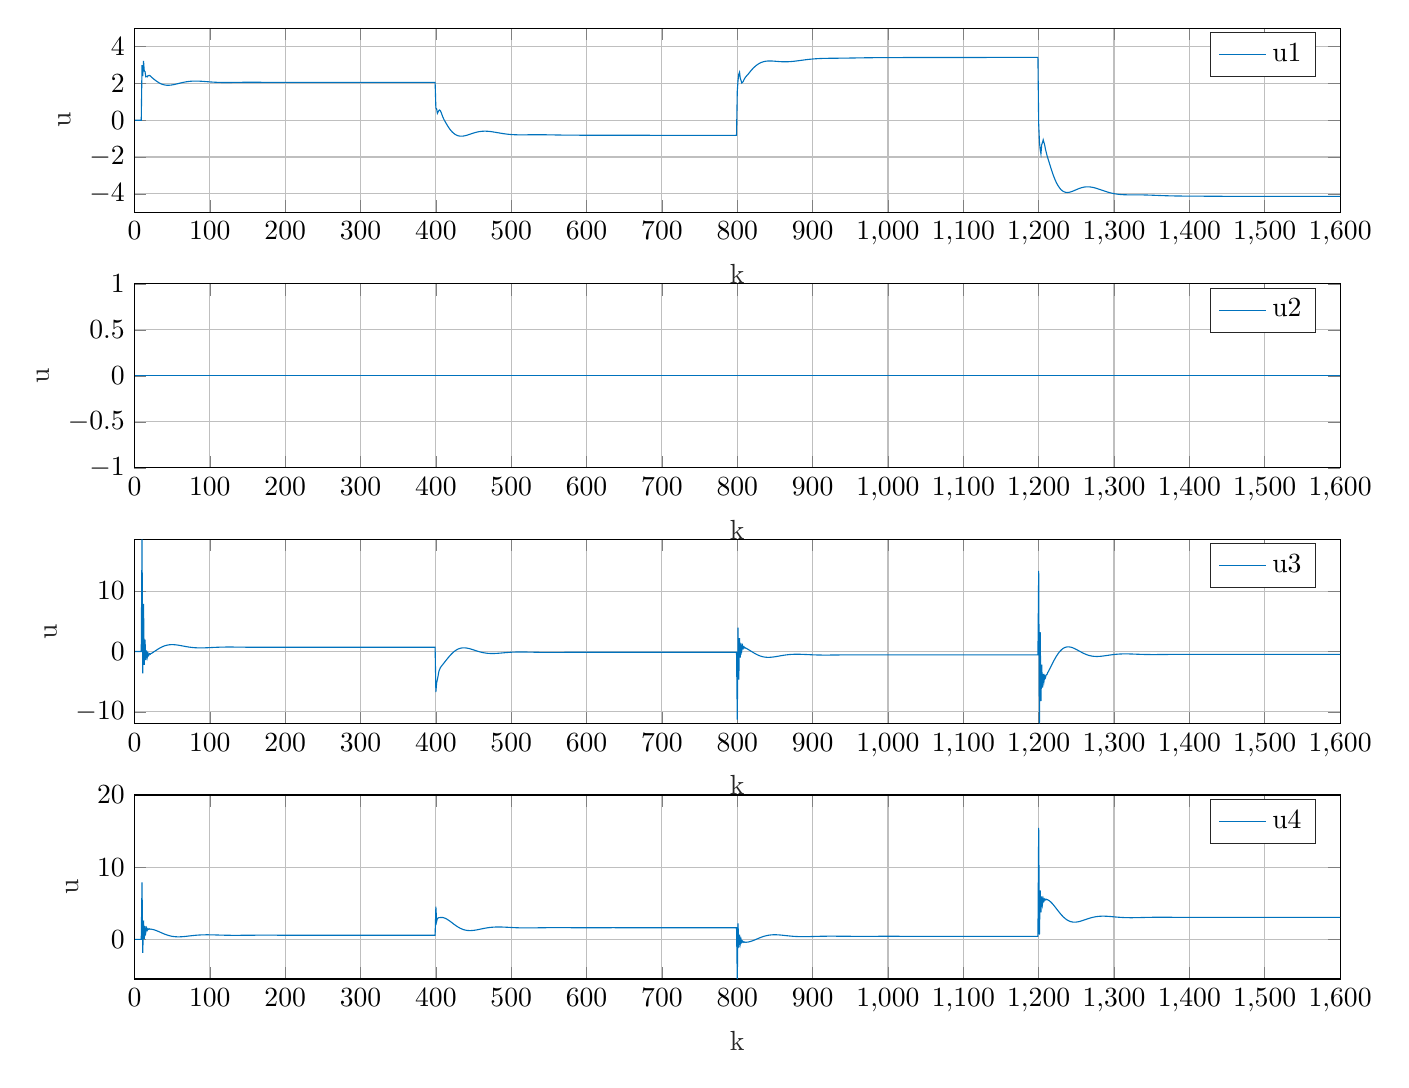
\begin{tikzpicture}

\begin{axis}[%
width=6.028in,
height=0.92in,
at={(1.011in,4.476in)},
scale only axis,
xmin=0,
xmax=1600,
xlabel style={font=\color{white!15!black}},
xlabel={k},
ymin=-5,
ymax=5,
ylabel style={font=\color{white!15!black}},
ylabel={u},
axis background/.style={fill=white},
xmajorgrids,
ymajorgrids,
legend style={legend cell align=left, align=left, draw=white!15!black}
]
\addplot [color=mycolor1]
  table[row sep=crcr]{%
1	0\\
2	0\\
3	0\\
4	0\\
5	0\\
6	0\\
7	0\\
8	0\\
9	0\\
10	2.9925\\
11	2.3995\\
12	3.2256\\
13	2.6804\\
14	2.645\\
15	2.3604\\
16	2.3806\\
17	2.3571\\
18	2.4217\\
19	2.43\\
20	2.4358\\
21	2.4048\\
22	2.3706\\
23	2.3285\\
24	2.2915\\
25	2.2559\\
26	2.2238\\
27	2.1922\\
28	2.1616\\
29	2.1314\\
30	2.1022\\
31	2.0745\\
32	2.0486\\
33	2.0247\\
34	2.0031\\
35	1.9835\\
36	1.9662\\
37	1.9509\\
38	1.9378\\
39	1.9267\\
40	1.9176\\
41	1.9106\\
42	1.9054\\
43	1.902\\
44	1.9003\\
45	1.9003\\
46	1.9017\\
47	1.9045\\
48	1.9085\\
49	1.9137\\
50	1.9199\\
51	1.927\\
52	1.9349\\
53	1.9434\\
54	1.9525\\
55	1.962\\
56	1.9718\\
57	1.9818\\
58	1.9919\\
59	2.0021\\
60	2.0122\\
61	2.0222\\
62	2.032\\
63	2.0415\\
64	2.0507\\
65	2.0594\\
66	2.0678\\
67	2.0757\\
68	2.083\\
69	2.0899\\
70	2.0961\\
71	2.1018\\
72	2.1069\\
73	2.1115\\
74	2.1154\\
75	2.1188\\
76	2.1216\\
77	2.1239\\
78	2.1256\\
79	2.1268\\
80	2.1275\\
81	2.1277\\
82	2.1275\\
83	2.1269\\
84	2.1259\\
85	2.1245\\
86	2.1228\\
87	2.1209\\
88	2.1186\\
89	2.1162\\
90	2.1135\\
91	2.1107\\
92	2.1078\\
93	2.1048\\
94	2.1017\\
95	2.0985\\
96	2.0953\\
97	2.0922\\
98	2.089\\
99	2.0859\\
100	2.0829\\
101	2.08\\
102	2.0771\\
103	2.0744\\
104	2.0718\\
105	2.0693\\
106	2.067\\
107	2.0649\\
108	2.0628\\
109	2.061\\
110	2.0593\\
111	2.0578\\
112	2.0564\\
113	2.0552\\
114	2.0541\\
115	2.0532\\
116	2.0525\\
117	2.0519\\
118	2.0514\\
119	2.0511\\
120	2.0508\\
121	2.0507\\
122	2.0507\\
123	2.0508\\
124	2.051\\
125	2.0513\\
126	2.0516\\
127	2.052\\
128	2.0525\\
129	2.053\\
130	2.0535\\
131	2.0541\\
132	2.0547\\
133	2.0553\\
134	2.0559\\
135	2.0565\\
136	2.0571\\
137	2.0577\\
138	2.0583\\
139	2.0589\\
140	2.0594\\
141	2.0599\\
142	2.0604\\
143	2.0609\\
144	2.0613\\
145	2.0616\\
146	2.062\\
147	2.0623\\
148	2.0626\\
149	2.0628\\
150	2.063\\
151	2.0631\\
152	2.0632\\
153	2.0633\\
154	2.0633\\
155	2.0633\\
156	2.0633\\
157	2.0632\\
158	2.0631\\
159	2.063\\
160	2.0628\\
161	2.0627\\
162	2.0625\\
163	2.0623\\
164	2.062\\
165	2.0618\\
166	2.0615\\
167	2.0613\\
168	2.061\\
169	2.0607\\
170	2.0605\\
171	2.0602\\
172	2.0599\\
173	2.0596\\
174	2.0594\\
175	2.0591\\
176	2.0588\\
177	2.0586\\
178	2.0583\\
179	2.0581\\
180	2.0579\\
181	2.0577\\
182	2.0575\\
183	2.0573\\
184	2.0571\\
185	2.0569\\
186	2.0568\\
187	2.0567\\
188	2.0565\\
189	2.0564\\
190	2.0563\\
191	2.0562\\
192	2.0561\\
193	2.0561\\
194	2.056\\
195	2.056\\
196	2.0559\\
197	2.0559\\
198	2.0559\\
199	2.0558\\
200	2.0558\\
201	2.0558\\
202	2.0558\\
203	2.0558\\
204	2.0558\\
205	2.0559\\
206	2.0559\\
207	2.0559\\
208	2.0559\\
209	2.0559\\
210	2.056\\
211	2.056\\
212	2.056\\
213	2.056\\
214	2.056\\
215	2.0561\\
216	2.0561\\
217	2.0561\\
218	2.0561\\
219	2.0561\\
220	2.0561\\
221	2.0562\\
222	2.0562\\
223	2.0562\\
224	2.0562\\
225	2.0562\\
226	2.0562\\
227	2.0562\\
228	2.0562\\
229	2.0561\\
230	2.0561\\
231	2.0561\\
232	2.0561\\
233	2.0561\\
234	2.0561\\
235	2.056\\
236	2.056\\
237	2.056\\
238	2.056\\
239	2.0559\\
240	2.0559\\
241	2.0559\\
242	2.0559\\
243	2.0558\\
244	2.0558\\
245	2.0558\\
246	2.0557\\
247	2.0557\\
248	2.0557\\
249	2.0557\\
250	2.0556\\
251	2.0556\\
252	2.0556\\
253	2.0555\\
254	2.0555\\
255	2.0555\\
256	2.0555\\
257	2.0555\\
258	2.0554\\
259	2.0554\\
260	2.0554\\
261	2.0554\\
262	2.0554\\
263	2.0553\\
264	2.0553\\
265	2.0553\\
266	2.0553\\
267	2.0553\\
268	2.0553\\
269	2.0553\\
270	2.0553\\
271	2.0553\\
272	2.0552\\
273	2.0552\\
274	2.0552\\
275	2.0552\\
276	2.0552\\
277	2.0552\\
278	2.0552\\
279	2.0552\\
280	2.0552\\
281	2.0552\\
282	2.0552\\
283	2.0552\\
284	2.0552\\
285	2.0552\\
286	2.0552\\
287	2.0552\\
288	2.0552\\
289	2.0552\\
290	2.0552\\
291	2.0552\\
292	2.0552\\
293	2.0552\\
294	2.0552\\
295	2.0552\\
296	2.0552\\
297	2.0552\\
298	2.0552\\
299	2.0552\\
300	2.0552\\
301	2.0552\\
302	2.0552\\
303	2.0551\\
304	2.0551\\
305	2.0551\\
306	2.0551\\
307	2.0551\\
308	2.0551\\
309	2.0551\\
310	2.0551\\
311	2.0551\\
312	2.0551\\
313	2.0551\\
314	2.0551\\
315	2.0551\\
316	2.0551\\
317	2.0551\\
318	2.0551\\
319	2.0551\\
320	2.0551\\
321	2.0551\\
322	2.0551\\
323	2.0551\\
324	2.0551\\
325	2.0551\\
326	2.0551\\
327	2.0551\\
328	2.0551\\
329	2.0551\\
330	2.0551\\
331	2.055\\
332	2.055\\
333	2.055\\
334	2.055\\
335	2.055\\
336	2.055\\
337	2.055\\
338	2.055\\
339	2.055\\
340	2.055\\
341	2.055\\
342	2.055\\
343	2.055\\
344	2.055\\
345	2.055\\
346	2.055\\
347	2.055\\
348	2.055\\
349	2.055\\
350	2.055\\
351	2.055\\
352	2.055\\
353	2.055\\
354	2.055\\
355	2.055\\
356	2.055\\
357	2.055\\
358	2.055\\
359	2.055\\
360	2.055\\
361	2.055\\
362	2.055\\
363	2.055\\
364	2.055\\
365	2.055\\
366	2.055\\
367	2.055\\
368	2.055\\
369	2.055\\
370	2.055\\
371	2.055\\
372	2.055\\
373	2.055\\
374	2.055\\
375	2.055\\
376	2.055\\
377	2.055\\
378	2.055\\
379	2.055\\
380	2.055\\
381	2.055\\
382	2.055\\
383	2.055\\
384	2.055\\
385	2.055\\
386	2.055\\
387	2.055\\
388	2.055\\
389	2.055\\
390	2.055\\
391	2.055\\
392	2.055\\
393	2.055\\
394	2.055\\
395	2.055\\
396	2.055\\
397	2.055\\
398	2.055\\
399	2.055\\
400	0.65847\\
401	0.62581\\
402	0.37197\\
403	0.45098\\
404	0.52733\\
405	0.55922\\
406	0.5172\\
407	0.42284\\
408	0.30966\\
409	0.19969\\
410	0.10357\\
411	0.020186\\
412	-0.054865\\
413	-0.12631\\
414	-0.19633\\
415	-0.26523\\
416	-0.33203\\
417	-0.39564\\
418	-0.45524\\
419	-0.5105\\
420	-0.56137\\
421	-0.60796\\
422	-0.6504\\
423	-0.68876\\
424	-0.72309\\
425	-0.75344\\
426	-0.77987\\
427	-0.80248\\
428	-0.82139\\
429	-0.83677\\
430	-0.84879\\
431	-0.85763\\
432	-0.8635\\
433	-0.86659\\
434	-0.86712\\
435	-0.86529\\
436	-0.86134\\
437	-0.85546\\
438	-0.84789\\
439	-0.83884\\
440	-0.82853\\
441	-0.81714\\
442	-0.8049\\
443	-0.79199\\
444	-0.77859\\
445	-0.76487\\
446	-0.75101\\
447	-0.73715\\
448	-0.72344\\
449	-0.71001\\
450	-0.69698\\
451	-0.68444\\
452	-0.67251\\
453	-0.66126\\
454	-0.65076\\
455	-0.64108\\
456	-0.63226\\
457	-0.62434\\
458	-0.61735\\
459	-0.61131\\
460	-0.60622\\
461	-0.60209\\
462	-0.59891\\
463	-0.59667\\
464	-0.59533\\
465	-0.59488\\
466	-0.59527\\
467	-0.59648\\
468	-0.59845\\
469	-0.60115\\
470	-0.60451\\
471	-0.6085\\
472	-0.61305\\
473	-0.6181\\
474	-0.62362\\
475	-0.62953\\
476	-0.63578\\
477	-0.64233\\
478	-0.6491\\
479	-0.65606\\
480	-0.66314\\
481	-0.67031\\
482	-0.67751\\
483	-0.6847\\
484	-0.69184\\
485	-0.6989\\
486	-0.70582\\
487	-0.71259\\
488	-0.71918\\
489	-0.72555\\
490	-0.73169\\
491	-0.73757\\
492	-0.74317\\
493	-0.7485\\
494	-0.75352\\
495	-0.75824\\
496	-0.76265\\
497	-0.76675\\
498	-0.77053\\
499	-0.774\\
500	-0.77716\\
501	-0.78002\\
502	-0.78259\\
503	-0.78486\\
504	-0.78687\\
505	-0.78861\\
506	-0.7901\\
507	-0.79135\\
508	-0.79238\\
509	-0.7932\\
510	-0.79383\\
511	-0.79429\\
512	-0.79459\\
513	-0.79474\\
514	-0.79476\\
515	-0.79467\\
516	-0.79449\\
517	-0.79422\\
518	-0.79388\\
519	-0.79349\\
520	-0.79306\\
521	-0.7926\\
522	-0.79212\\
523	-0.79164\\
524	-0.79116\\
525	-0.79069\\
526	-0.79024\\
527	-0.78982\\
528	-0.78944\\
529	-0.7891\\
530	-0.78881\\
531	-0.78856\\
532	-0.78837\\
533	-0.78824\\
534	-0.78816\\
535	-0.78815\\
536	-0.78819\\
537	-0.78829\\
538	-0.78846\\
539	-0.78868\\
540	-0.78896\\
541	-0.78929\\
542	-0.78967\\
543	-0.79011\\
544	-0.79059\\
545	-0.79111\\
546	-0.79167\\
547	-0.79227\\
548	-0.7929\\
549	-0.79356\\
550	-0.79425\\
551	-0.79495\\
552	-0.79567\\
553	-0.79641\\
554	-0.79715\\
555	-0.7979\\
556	-0.79865\\
557	-0.7994\\
558	-0.80015\\
559	-0.80089\\
560	-0.80162\\
561	-0.80233\\
562	-0.80303\\
563	-0.80372\\
564	-0.80439\\
565	-0.80503\\
566	-0.80566\\
567	-0.80626\\
568	-0.80684\\
569	-0.80739\\
570	-0.80792\\
571	-0.80842\\
572	-0.80889\\
573	-0.80934\\
574	-0.80976\\
575	-0.81016\\
576	-0.81053\\
577	-0.81088\\
578	-0.8112\\
579	-0.8115\\
580	-0.81178\\
581	-0.81203\\
582	-0.81227\\
583	-0.81248\\
584	-0.81268\\
585	-0.81286\\
586	-0.81302\\
587	-0.81317\\
588	-0.81331\\
589	-0.81343\\
590	-0.81354\\
591	-0.81365\\
592	-0.81374\\
593	-0.81382\\
594	-0.8139\\
595	-0.81397\\
596	-0.81404\\
597	-0.8141\\
598	-0.81417\\
599	-0.81422\\
600	-0.81428\\
601	-0.81434\\
602	-0.81439\\
603	-0.81445\\
604	-0.81451\\
605	-0.81457\\
606	-0.81463\\
607	-0.81469\\
608	-0.81475\\
609	-0.81482\\
610	-0.81489\\
611	-0.81496\\
612	-0.81503\\
613	-0.81511\\
614	-0.81519\\
615	-0.81528\\
616	-0.81536\\
617	-0.81545\\
618	-0.81554\\
619	-0.81563\\
620	-0.81572\\
621	-0.81582\\
622	-0.81592\\
623	-0.81602\\
624	-0.81612\\
625	-0.81622\\
626	-0.81632\\
627	-0.81642\\
628	-0.81652\\
629	-0.81662\\
630	-0.81672\\
631	-0.81682\\
632	-0.81692\\
633	-0.81701\\
634	-0.81711\\
635	-0.8172\\
636	-0.8173\\
637	-0.81739\\
638	-0.81747\\
639	-0.81756\\
640	-0.81765\\
641	-0.81773\\
642	-0.81781\\
643	-0.81788\\
644	-0.81796\\
645	-0.81803\\
646	-0.8181\\
647	-0.81817\\
648	-0.81823\\
649	-0.81829\\
650	-0.81835\\
651	-0.81841\\
652	-0.81846\\
653	-0.81852\\
654	-0.81857\\
655	-0.81861\\
656	-0.81866\\
657	-0.8187\\
658	-0.81874\\
659	-0.81878\\
660	-0.81882\\
661	-0.81886\\
662	-0.81889\\
663	-0.81892\\
664	-0.81895\\
665	-0.81898\\
666	-0.81901\\
667	-0.81904\\
668	-0.81906\\
669	-0.81909\\
670	-0.81911\\
671	-0.81914\\
672	-0.81916\\
673	-0.81918\\
674	-0.81921\\
675	-0.81923\\
676	-0.81925\\
677	-0.81927\\
678	-0.81929\\
679	-0.81931\\
680	-0.81933\\
681	-0.81935\\
682	-0.81937\\
683	-0.81938\\
684	-0.8194\\
685	-0.81942\\
686	-0.81944\\
687	-0.81946\\
688	-0.81948\\
689	-0.81949\\
690	-0.81951\\
691	-0.81953\\
692	-0.81955\\
693	-0.81957\\
694	-0.81958\\
695	-0.8196\\
696	-0.81962\\
697	-0.81964\\
698	-0.81965\\
699	-0.81967\\
700	-0.81969\\
701	-0.8197\\
702	-0.81972\\
703	-0.81974\\
704	-0.81975\\
705	-0.81977\\
706	-0.81978\\
707	-0.8198\\
708	-0.81982\\
709	-0.81983\\
710	-0.81984\\
711	-0.81986\\
712	-0.81987\\
713	-0.81989\\
714	-0.8199\\
715	-0.81991\\
716	-0.81993\\
717	-0.81994\\
718	-0.81995\\
719	-0.81996\\
720	-0.81997\\
721	-0.81999\\
722	-0.82\\
723	-0.82001\\
724	-0.82002\\
725	-0.82003\\
726	-0.82004\\
727	-0.82005\\
728	-0.82005\\
729	-0.82006\\
730	-0.82007\\
731	-0.82008\\
732	-0.82009\\
733	-0.8201\\
734	-0.8201\\
735	-0.82011\\
736	-0.82012\\
737	-0.82012\\
738	-0.82013\\
739	-0.82014\\
740	-0.82014\\
741	-0.82015\\
742	-0.82016\\
743	-0.82016\\
744	-0.82017\\
745	-0.82017\\
746	-0.82018\\
747	-0.82018\\
748	-0.82019\\
749	-0.82019\\
750	-0.8202\\
751	-0.8202\\
752	-0.82021\\
753	-0.82021\\
754	-0.82021\\
755	-0.82022\\
756	-0.82022\\
757	-0.82023\\
758	-0.82023\\
759	-0.82024\\
760	-0.82024\\
761	-0.82024\\
762	-0.82025\\
763	-0.82025\\
764	-0.82025\\
765	-0.82026\\
766	-0.82026\\
767	-0.82026\\
768	-0.82027\\
769	-0.82027\\
770	-0.82027\\
771	-0.82028\\
772	-0.82028\\
773	-0.82028\\
774	-0.82029\\
775	-0.82029\\
776	-0.82029\\
777	-0.8203\\
778	-0.8203\\
779	-0.8203\\
780	-0.82031\\
781	-0.82031\\
782	-0.82031\\
783	-0.82031\\
784	-0.82032\\
785	-0.82032\\
786	-0.82032\\
787	-0.82032\\
788	-0.82033\\
789	-0.82033\\
790	-0.82033\\
791	-0.82033\\
792	-0.82033\\
793	-0.82034\\
794	-0.82034\\
795	-0.82034\\
796	-0.82034\\
797	-0.82034\\
798	-0.82035\\
799	-0.82035\\
800	1.5737\\
801	2.1684\\
802	2.4974\\
803	2.6067\\
804	2.2751\\
805	2.158\\
806	2.0205\\
807	2.063\\
808	2.1156\\
809	2.2122\\
810	2.2817\\
811	2.3458\\
812	2.3923\\
813	2.4385\\
814	2.4835\\
815	2.5326\\
816	2.5829\\
817	2.6341\\
818	2.6837\\
819	2.7315\\
820	2.7768\\
821	2.8198\\
822	2.8605\\
823	2.899\\
824	2.9353\\
825	2.9693\\
826	3.001\\
827	3.0303\\
828	3.0571\\
829	3.0816\\
830	3.1038\\
831	3.1237\\
832	3.1414\\
833	3.157\\
834	3.1706\\
835	3.1823\\
836	3.1922\\
837	3.2004\\
838	3.207\\
839	3.2122\\
840	3.216\\
841	3.2186\\
842	3.2201\\
843	3.2206\\
844	3.2203\\
845	3.2192\\
846	3.2175\\
847	3.2153\\
848	3.2127\\
849	3.2098\\
850	3.2066\\
851	3.2033\\
852	3.1999\\
853	3.1966\\
854	3.1933\\
855	3.1902\\
856	3.1873\\
857	3.1847\\
858	3.1823\\
859	3.1803\\
860	3.1787\\
861	3.1774\\
862	3.1766\\
863	3.1762\\
864	3.1762\\
865	3.1767\\
866	3.1776\\
867	3.1789\\
868	3.1807\\
869	3.1829\\
870	3.1855\\
871	3.1884\\
872	3.1917\\
873	3.1954\\
874	3.1993\\
875	3.2036\\
876	3.2081\\
877	3.2128\\
878	3.2178\\
879	3.2229\\
880	3.2281\\
881	3.2335\\
882	3.239\\
883	3.2445\\
884	3.2501\\
885	3.2556\\
886	3.2612\\
887	3.2667\\
888	3.2722\\
889	3.2776\\
890	3.2828\\
891	3.288\\
892	3.2931\\
893	3.298\\
894	3.3027\\
895	3.3073\\
896	3.3117\\
897	3.3159\\
898	3.3199\\
899	3.3238\\
900	3.3274\\
901	3.3309\\
902	3.3342\\
903	3.3372\\
904	3.3401\\
905	3.3428\\
906	3.3453\\
907	3.3476\\
908	3.3497\\
909	3.3517\\
910	3.3535\\
911	3.3552\\
912	3.3567\\
913	3.3581\\
914	3.3594\\
915	3.3605\\
916	3.3616\\
917	3.3625\\
918	3.3634\\
919	3.3641\\
920	3.3648\\
921	3.3654\\
922	3.366\\
923	3.3665\\
924	3.367\\
925	3.3675\\
926	3.3679\\
927	3.3683\\
928	3.3687\\
929	3.3691\\
930	3.3694\\
931	3.3698\\
932	3.3702\\
933	3.3706\\
934	3.371\\
935	3.3714\\
936	3.3718\\
937	3.3722\\
938	3.3727\\
939	3.3732\\
940	3.3737\\
941	3.3742\\
942	3.3747\\
943	3.3753\\
944	3.3759\\
945	3.3765\\
946	3.3771\\
947	3.3778\\
948	3.3784\\
949	3.3791\\
950	3.3798\\
951	3.3805\\
952	3.3812\\
953	3.3819\\
954	3.3826\\
955	3.3833\\
956	3.384\\
957	3.3848\\
958	3.3855\\
959	3.3862\\
960	3.3869\\
961	3.3876\\
962	3.3883\\
963	3.389\\
964	3.3897\\
965	3.3903\\
966	3.391\\
967	3.3916\\
968	3.3922\\
969	3.3929\\
970	3.3934\\
971	3.394\\
972	3.3946\\
973	3.3951\\
974	3.3956\\
975	3.3961\\
976	3.3966\\
977	3.397\\
978	3.3975\\
979	3.3979\\
980	3.3983\\
981	3.3987\\
982	3.399\\
983	3.3994\\
984	3.3997\\
985	3.4\\
986	3.4003\\
987	3.4006\\
988	3.4009\\
989	3.4012\\
990	3.4014\\
991	3.4016\\
992	3.4019\\
993	3.4021\\
994	3.4023\\
995	3.4025\\
996	3.4027\\
997	3.4029\\
998	3.403\\
999	3.4032\\
1000	3.4034\\
1001	3.4035\\
1002	3.4037\\
1003	3.4038\\
1004	3.404\\
1005	3.4041\\
1006	3.4043\\
1007	3.4044\\
1008	3.4045\\
1009	3.4047\\
1010	3.4048\\
1011	3.4049\\
1012	3.4051\\
1013	3.4052\\
1014	3.4053\\
1015	3.4054\\
1016	3.4056\\
1017	3.4057\\
1018	3.4058\\
1019	3.406\\
1020	3.4061\\
1021	3.4062\\
1022	3.4063\\
1023	3.4065\\
1024	3.4066\\
1025	3.4067\\
1026	3.4068\\
1027	3.4069\\
1028	3.4071\\
1029	3.4072\\
1030	3.4073\\
1031	3.4074\\
1032	3.4075\\
1033	3.4076\\
1034	3.4078\\
1035	3.4079\\
1036	3.408\\
1037	3.4081\\
1038	3.4082\\
1039	3.4083\\
1040	3.4084\\
1041	3.4085\\
1042	3.4086\\
1043	3.4087\\
1044	3.4088\\
1045	3.4089\\
1046	3.409\\
1047	3.409\\
1048	3.4091\\
1049	3.4092\\
1050	3.4093\\
1051	3.4094\\
1052	3.4094\\
1053	3.4095\\
1054	3.4096\\
1055	3.4096\\
1056	3.4097\\
1057	3.4098\\
1058	3.4098\\
1059	3.4099\\
1060	3.41\\
1061	3.41\\
1062	3.4101\\
1063	3.4101\\
1064	3.4102\\
1065	3.4102\\
1066	3.4103\\
1067	3.4103\\
1068	3.4104\\
1069	3.4104\\
1070	3.4104\\
1071	3.4105\\
1072	3.4105\\
1073	3.4106\\
1074	3.4106\\
1075	3.4106\\
1076	3.4107\\
1077	3.4107\\
1078	3.4107\\
1079	3.4108\\
1080	3.4108\\
1081	3.4108\\
1082	3.4109\\
1083	3.4109\\
1084	3.4109\\
1085	3.4109\\
1086	3.411\\
1087	3.411\\
1088	3.411\\
1089	3.4111\\
1090	3.4111\\
1091	3.4111\\
1092	3.4111\\
1093	3.4112\\
1094	3.4112\\
1095	3.4112\\
1096	3.4112\\
1097	3.4113\\
1098	3.4113\\
1099	3.4113\\
1100	3.4113\\
1101	3.4114\\
1102	3.4114\\
1103	3.4114\\
1104	3.4114\\
1105	3.4114\\
1106	3.4115\\
1107	3.4115\\
1108	3.4115\\
1109	3.4115\\
1110	3.4115\\
1111	3.4116\\
1112	3.4116\\
1113	3.4116\\
1114	3.4116\\
1115	3.4116\\
1116	3.4116\\
1117	3.4117\\
1118	3.4117\\
1119	3.4117\\
1120	3.4117\\
1121	3.4117\\
1122	3.4117\\
1123	3.4118\\
1124	3.4118\\
1125	3.4118\\
1126	3.4118\\
1127	3.4118\\
1128	3.4118\\
1129	3.4118\\
1130	3.4118\\
1131	3.4119\\
1132	3.4119\\
1133	3.4119\\
1134	3.4119\\
1135	3.4119\\
1136	3.4119\\
1137	3.4119\\
1138	3.4119\\
1139	3.4119\\
1140	3.4119\\
1141	3.412\\
1142	3.412\\
1143	3.412\\
1144	3.412\\
1145	3.412\\
1146	3.412\\
1147	3.412\\
1148	3.412\\
1149	3.412\\
1150	3.412\\
1151	3.412\\
1152	3.412\\
1153	3.4121\\
1154	3.4121\\
1155	3.4121\\
1156	3.4121\\
1157	3.4121\\
1158	3.4121\\
1159	3.4121\\
1160	3.4121\\
1161	3.4121\\
1162	3.4121\\
1163	3.4121\\
1164	3.4121\\
1165	3.4121\\
1166	3.4121\\
1167	3.4121\\
1168	3.4121\\
1169	3.4121\\
1170	3.4121\\
1171	3.4121\\
1172	3.4122\\
1173	3.4122\\
1174	3.4122\\
1175	3.4122\\
1176	3.4122\\
1177	3.4122\\
1178	3.4122\\
1179	3.4122\\
1180	3.4122\\
1181	3.4122\\
1182	3.4122\\
1183	3.4122\\
1184	3.4122\\
1185	3.4122\\
1186	3.4122\\
1187	3.4122\\
1188	3.4122\\
1189	3.4122\\
1190	3.4122\\
1191	3.4122\\
1192	3.4122\\
1193	3.4122\\
1194	3.4122\\
1195	3.4122\\
1196	3.4122\\
1197	3.4122\\
1198	3.4122\\
1199	3.4122\\
1200	-0.17875\\
1201	-1.17\\
1202	-1.6032\\
1203	-1.8323\\
1204	-1.3298\\
1205	-1.2215\\
1206	-1.0646\\
1207	-1.2065\\
1208	-1.3539\\
1209	-1.5733\\
1210	-1.7453\\
1211	-1.9092\\
1212	-2.0434\\
1213	-2.1764\\
1214	-2.3051\\
1215	-2.4381\\
1216	-2.57\\
1217	-2.7003\\
1218	-2.8249\\
1219	-2.9434\\
1220	-3.0546\\
1221	-3.1587\\
1222	-3.2559\\
1223	-3.3461\\
1224	-3.4295\\
1225	-3.5059\\
1226	-3.5752\\
1227	-3.6376\\
1228	-3.6931\\
1229	-3.742\\
1230	-3.7843\\
1231	-3.8204\\
1232	-3.8507\\
1233	-3.8753\\
1234	-3.8946\\
1235	-3.9089\\
1236	-3.9186\\
1237	-3.9241\\
1238	-3.9257\\
1239	-3.9238\\
1240	-3.9188\\
1241	-3.911\\
1242	-3.9008\\
1243	-3.8886\\
1244	-3.8747\\
1245	-3.8593\\
1246	-3.8429\\
1247	-3.8258\\
1248	-3.8082\\
1249	-3.7904\\
1250	-3.7726\\
1251	-3.7551\\
1252	-3.738\\
1253	-3.7216\\
1254	-3.7061\\
1255	-3.6915\\
1256	-3.6781\\
1257	-3.6658\\
1258	-3.6549\\
1259	-3.6454\\
1260	-3.6373\\
1261	-3.6306\\
1262	-3.6255\\
1263	-3.6219\\
1264	-3.6198\\
1265	-3.6191\\
1266	-3.6199\\
1267	-3.6221\\
1268	-3.6257\\
1269	-3.6305\\
1270	-3.6366\\
1271	-3.6438\\
1272	-3.6521\\
1273	-3.6614\\
1274	-3.6716\\
1275	-3.6826\\
1276	-3.6943\\
1277	-3.7067\\
1278	-3.7195\\
1279	-3.7329\\
1280	-3.7466\\
1281	-3.7605\\
1282	-3.7746\\
1283	-3.7889\\
1284	-3.8032\\
1285	-3.8174\\
1286	-3.8315\\
1287	-3.8454\\
1288	-3.8591\\
1289	-3.8725\\
1290	-3.8855\\
1291	-3.8981\\
1292	-3.9104\\
1293	-3.9221\\
1294	-3.9334\\
1295	-3.9442\\
1296	-3.9544\\
1297	-3.9641\\
1298	-3.9732\\
1299	-3.9818\\
1300	-3.9898\\
1301	-3.9972\\
1302	-4.0041\\
1303	-4.0105\\
1304	-4.0163\\
1305	-4.0216\\
1306	-4.0265\\
1307	-4.0308\\
1308	-4.0347\\
1309	-4.0381\\
1310	-4.0412\\
1311	-4.0438\\
1312	-4.0461\\
1313	-4.0481\\
1314	-4.0498\\
1315	-4.0512\\
1316	-4.0524\\
1317	-4.0533\\
1318	-4.0541\\
1319	-4.0546\\
1320	-4.0551\\
1321	-4.0554\\
1322	-4.0556\\
1323	-4.0558\\
1324	-4.0559\\
1325	-4.0559\\
1326	-4.056\\
1327	-4.056\\
1328	-4.056\\
1329	-4.0561\\
1330	-4.0562\\
1331	-4.0564\\
1332	-4.0566\\
1333	-4.0569\\
1334	-4.0573\\
1335	-4.0577\\
1336	-4.0582\\
1337	-4.0588\\
1338	-4.0595\\
1339	-4.0603\\
1340	-4.0611\\
1341	-4.0621\\
1342	-4.0631\\
1343	-4.0642\\
1344	-4.0654\\
1345	-4.0667\\
1346	-4.068\\
1347	-4.0693\\
1348	-4.0708\\
1349	-4.0723\\
1350	-4.0738\\
1351	-4.0754\\
1352	-4.077\\
1353	-4.0786\\
1354	-4.0802\\
1355	-4.0819\\
1356	-4.0836\\
1357	-4.0852\\
1358	-4.0869\\
1359	-4.0886\\
1360	-4.0902\\
1361	-4.0918\\
1362	-4.0934\\
1363	-4.095\\
1364	-4.0965\\
1365	-4.098\\
1366	-4.0995\\
1367	-4.1009\\
1368	-4.1023\\
1369	-4.1036\\
1370	-4.1049\\
1371	-4.1062\\
1372	-4.1074\\
1373	-4.1085\\
1374	-4.1096\\
1375	-4.1106\\
1376	-4.1116\\
1377	-4.1126\\
1378	-4.1135\\
1379	-4.1143\\
1380	-4.1151\\
1381	-4.1159\\
1382	-4.1166\\
1383	-4.1172\\
1384	-4.1179\\
1385	-4.1185\\
1386	-4.119\\
1387	-4.1195\\
1388	-4.12\\
1389	-4.1205\\
1390	-4.1209\\
1391	-4.1213\\
1392	-4.1217\\
1393	-4.1221\\
1394	-4.1224\\
1395	-4.1227\\
1396	-4.123\\
1397	-4.1233\\
1398	-4.1236\\
1399	-4.1239\\
1400	-4.1241\\
1401	-4.1244\\
1402	-4.1246\\
1403	-4.1249\\
1404	-4.1251\\
1405	-4.1254\\
1406	-4.1256\\
1407	-4.1258\\
1408	-4.1261\\
1409	-4.1263\\
1410	-4.1265\\
1411	-4.1268\\
1412	-4.127\\
1413	-4.1272\\
1414	-4.1275\\
1415	-4.1277\\
1416	-4.128\\
1417	-4.1282\\
1418	-4.1285\\
1419	-4.1287\\
1420	-4.129\\
1421	-4.1292\\
1422	-4.1295\\
1423	-4.1297\\
1424	-4.13\\
1425	-4.1302\\
1426	-4.1305\\
1427	-4.1307\\
1428	-4.131\\
1429	-4.1312\\
1430	-4.1315\\
1431	-4.1317\\
1432	-4.132\\
1433	-4.1322\\
1434	-4.1325\\
1435	-4.1327\\
1436	-4.1329\\
1437	-4.1332\\
1438	-4.1334\\
1439	-4.1336\\
1440	-4.1338\\
1441	-4.134\\
1442	-4.1342\\
1443	-4.1344\\
1444	-4.1346\\
1445	-4.1348\\
1446	-4.135\\
1447	-4.1352\\
1448	-4.1353\\
1449	-4.1355\\
1450	-4.1357\\
1451	-4.1358\\
1452	-4.136\\
1453	-4.1361\\
1454	-4.1363\\
1455	-4.1364\\
1456	-4.1365\\
1457	-4.1366\\
1458	-4.1368\\
1459	-4.1369\\
1460	-4.137\\
1461	-4.1371\\
1462	-4.1372\\
1463	-4.1373\\
1464	-4.1374\\
1465	-4.1375\\
1466	-4.1376\\
1467	-4.1377\\
1468	-4.1377\\
1469	-4.1378\\
1470	-4.1379\\
1471	-4.138\\
1472	-4.1381\\
1473	-4.1381\\
1474	-4.1382\\
1475	-4.1383\\
1476	-4.1383\\
1477	-4.1384\\
1478	-4.1385\\
1479	-4.1385\\
1480	-4.1386\\
1481	-4.1386\\
1482	-4.1387\\
1483	-4.1387\\
1484	-4.1388\\
1485	-4.1389\\
1486	-4.1389\\
1487	-4.139\\
1488	-4.139\\
1489	-4.1391\\
1490	-4.1391\\
1491	-4.1392\\
1492	-4.1392\\
1493	-4.1393\\
1494	-4.1393\\
1495	-4.1394\\
1496	-4.1394\\
1497	-4.1395\\
1498	-4.1395\\
1499	-4.1396\\
1500	-4.1396\\
1501	-4.1397\\
1502	-4.1397\\
1503	-4.1397\\
1504	-4.1398\\
1505	-4.1398\\
1506	-4.1399\\
1507	-4.1399\\
1508	-4.14\\
1509	-4.14\\
1510	-4.14\\
1511	-4.1401\\
1512	-4.1401\\
1513	-4.1401\\
1514	-4.1402\\
1515	-4.1402\\
1516	-4.1403\\
1517	-4.1403\\
1518	-4.1403\\
1519	-4.1403\\
1520	-4.1404\\
1521	-4.1404\\
1522	-4.1404\\
1523	-4.1405\\
1524	-4.1405\\
1525	-4.1405\\
1526	-4.1406\\
1527	-4.1406\\
1528	-4.1406\\
1529	-4.1406\\
1530	-4.1407\\
1531	-4.1407\\
1532	-4.1407\\
1533	-4.1407\\
1534	-4.1407\\
1535	-4.1408\\
1536	-4.1408\\
1537	-4.1408\\
1538	-4.1408\\
1539	-4.1408\\
1540	-4.1409\\
1541	-4.1409\\
1542	-4.1409\\
1543	-4.1409\\
1544	-4.1409\\
1545	-4.1409\\
1546	-4.141\\
1547	-4.141\\
1548	-4.141\\
1549	-4.141\\
1550	-4.141\\
1551	-4.141\\
1552	-4.141\\
1553	-4.1411\\
1554	-4.1411\\
1555	-4.1411\\
1556	-4.1411\\
1557	-4.1411\\
1558	-4.1411\\
1559	-4.1411\\
1560	-4.1411\\
1561	-4.1411\\
1562	-4.1412\\
1563	-4.1412\\
1564	-4.1412\\
1565	-4.1412\\
1566	-4.1412\\
1567	-4.1412\\
1568	-4.1412\\
1569	-4.1412\\
1570	-4.1412\\
1571	-4.1412\\
1572	-4.1413\\
1573	-4.1413\\
1574	-4.1413\\
1575	-4.1413\\
1576	-4.1413\\
1577	-4.1413\\
1578	-4.1413\\
1579	-4.1413\\
1580	-4.1413\\
1581	-4.1413\\
1582	-4.1413\\
1583	-4.1413\\
1584	-4.1414\\
1585	-4.1414\\
1586	-4.1414\\
1587	-4.1414\\
1588	-4.1414\\
1589	-4.1414\\
1590	-4.1414\\
1591	-4.1414\\
1592	-4.1414\\
1593	-4.1414\\
1594	-4.1414\\
1595	-4.1414\\
1596	-4.1414\\
1597	-4.1414\\
1598	-4.1414\\
1599	-4.1414\\
1600	-4.1414\\
};
\addlegendentry{u1}

\end{axis}

\begin{axis}[%
width=6.028in,
height=0.92in,
at={(1.011in,3.198in)},
scale only axis,
xmin=0,
xmax=1600,
xlabel style={font=\color{white!15!black}},
xlabel={k},
ymin=-1,
ymax=1,
ylabel style={font=\color{white!15!black}},
ylabel={u},
axis background/.style={fill=white},
xmajorgrids,
ymajorgrids,
legend style={legend cell align=left, align=left, draw=white!15!black}
]
\addplot [color=mycolor1]
  table[row sep=crcr]{%
1	0\\
2	0\\
3	0\\
4	0\\
5	0\\
6	0\\
7	0\\
8	0\\
9	0\\
10	0\\
11	0\\
12	0\\
13	0\\
14	0\\
15	0\\
16	0\\
17	0\\
18	0\\
19	0\\
20	0\\
21	0\\
22	0\\
23	0\\
24	0\\
25	0\\
26	0\\
27	0\\
28	0\\
29	0\\
30	0\\
31	0\\
32	0\\
33	0\\
34	0\\
35	0\\
36	0\\
37	0\\
38	0\\
39	0\\
40	0\\
41	0\\
42	0\\
43	0\\
44	0\\
45	0\\
46	0\\
47	0\\
48	0\\
49	0\\
50	0\\
51	0\\
52	0\\
53	0\\
54	0\\
55	0\\
56	0\\
57	0\\
58	0\\
59	0\\
60	0\\
61	0\\
62	0\\
63	0\\
64	0\\
65	0\\
66	0\\
67	0\\
68	0\\
69	0\\
70	0\\
71	0\\
72	0\\
73	0\\
74	0\\
75	0\\
76	0\\
77	0\\
78	0\\
79	0\\
80	0\\
81	0\\
82	0\\
83	0\\
84	0\\
85	0\\
86	0\\
87	0\\
88	0\\
89	0\\
90	0\\
91	0\\
92	0\\
93	0\\
94	0\\
95	0\\
96	0\\
97	0\\
98	0\\
99	0\\
100	0\\
101	0\\
102	0\\
103	0\\
104	0\\
105	0\\
106	0\\
107	0\\
108	0\\
109	0\\
110	0\\
111	0\\
112	0\\
113	0\\
114	0\\
115	0\\
116	0\\
117	0\\
118	0\\
119	0\\
120	0\\
121	0\\
122	0\\
123	0\\
124	0\\
125	0\\
126	0\\
127	0\\
128	0\\
129	0\\
130	0\\
131	0\\
132	0\\
133	0\\
134	0\\
135	0\\
136	0\\
137	0\\
138	0\\
139	0\\
140	0\\
141	0\\
142	0\\
143	0\\
144	0\\
145	0\\
146	0\\
147	0\\
148	0\\
149	0\\
150	0\\
151	0\\
152	0\\
153	0\\
154	0\\
155	0\\
156	0\\
157	0\\
158	0\\
159	0\\
160	0\\
161	0\\
162	0\\
163	0\\
164	0\\
165	0\\
166	0\\
167	0\\
168	0\\
169	0\\
170	0\\
171	0\\
172	0\\
173	0\\
174	0\\
175	0\\
176	0\\
177	0\\
178	0\\
179	0\\
180	0\\
181	0\\
182	0\\
183	0\\
184	0\\
185	0\\
186	0\\
187	0\\
188	0\\
189	0\\
190	0\\
191	0\\
192	0\\
193	0\\
194	0\\
195	0\\
196	0\\
197	0\\
198	0\\
199	0\\
200	0\\
201	0\\
202	0\\
203	0\\
204	0\\
205	0\\
206	0\\
207	0\\
208	0\\
209	0\\
210	0\\
211	0\\
212	0\\
213	0\\
214	0\\
215	0\\
216	0\\
217	0\\
218	0\\
219	0\\
220	0\\
221	0\\
222	0\\
223	0\\
224	0\\
225	0\\
226	0\\
227	0\\
228	0\\
229	0\\
230	0\\
231	0\\
232	0\\
233	0\\
234	0\\
235	0\\
236	0\\
237	0\\
238	0\\
239	0\\
240	0\\
241	0\\
242	0\\
243	0\\
244	0\\
245	0\\
246	0\\
247	0\\
248	0\\
249	0\\
250	0\\
251	0\\
252	0\\
253	0\\
254	0\\
255	0\\
256	0\\
257	0\\
258	0\\
259	0\\
260	0\\
261	0\\
262	0\\
263	0\\
264	0\\
265	0\\
266	0\\
267	0\\
268	0\\
269	0\\
270	0\\
271	0\\
272	0\\
273	0\\
274	0\\
275	0\\
276	0\\
277	0\\
278	0\\
279	0\\
280	0\\
281	0\\
282	0\\
283	0\\
284	0\\
285	0\\
286	0\\
287	0\\
288	0\\
289	0\\
290	0\\
291	0\\
292	0\\
293	0\\
294	0\\
295	0\\
296	0\\
297	0\\
298	0\\
299	0\\
300	0\\
301	0\\
302	0\\
303	0\\
304	0\\
305	0\\
306	0\\
307	0\\
308	0\\
309	0\\
310	0\\
311	0\\
312	0\\
313	0\\
314	0\\
315	0\\
316	0\\
317	0\\
318	0\\
319	0\\
320	0\\
321	0\\
322	0\\
323	0\\
324	0\\
325	0\\
326	0\\
327	0\\
328	0\\
329	0\\
330	0\\
331	0\\
332	0\\
333	0\\
334	0\\
335	0\\
336	0\\
337	0\\
338	0\\
339	0\\
340	0\\
341	0\\
342	0\\
343	0\\
344	0\\
345	0\\
346	0\\
347	0\\
348	0\\
349	0\\
350	0\\
351	0\\
352	0\\
353	0\\
354	0\\
355	0\\
356	0\\
357	0\\
358	0\\
359	0\\
360	0\\
361	0\\
362	0\\
363	0\\
364	0\\
365	0\\
366	0\\
367	0\\
368	0\\
369	0\\
370	0\\
371	0\\
372	0\\
373	0\\
374	0\\
375	0\\
376	0\\
377	0\\
378	0\\
379	0\\
380	0\\
381	0\\
382	0\\
383	0\\
384	0\\
385	0\\
386	0\\
387	0\\
388	0\\
389	0\\
390	0\\
391	0\\
392	0\\
393	0\\
394	0\\
395	0\\
396	0\\
397	0\\
398	0\\
399	0\\
400	0\\
401	0\\
402	0\\
403	0\\
404	0\\
405	0\\
406	0\\
407	0\\
408	0\\
409	0\\
410	0\\
411	0\\
412	0\\
413	0\\
414	0\\
415	0\\
416	0\\
417	0\\
418	0\\
419	0\\
420	0\\
421	0\\
422	0\\
423	0\\
424	0\\
425	0\\
426	0\\
427	0\\
428	0\\
429	0\\
430	0\\
431	0\\
432	0\\
433	0\\
434	0\\
435	0\\
436	0\\
437	0\\
438	0\\
439	0\\
440	0\\
441	0\\
442	0\\
443	0\\
444	0\\
445	0\\
446	0\\
447	0\\
448	0\\
449	0\\
450	0\\
451	0\\
452	0\\
453	0\\
454	0\\
455	0\\
456	0\\
457	0\\
458	0\\
459	0\\
460	0\\
461	0\\
462	0\\
463	0\\
464	0\\
465	0\\
466	0\\
467	0\\
468	0\\
469	0\\
470	0\\
471	0\\
472	0\\
473	0\\
474	0\\
475	0\\
476	0\\
477	0\\
478	0\\
479	0\\
480	0\\
481	0\\
482	0\\
483	0\\
484	0\\
485	0\\
486	0\\
487	0\\
488	0\\
489	0\\
490	0\\
491	0\\
492	0\\
493	0\\
494	0\\
495	0\\
496	0\\
497	0\\
498	0\\
499	0\\
500	0\\
501	0\\
502	0\\
503	0\\
504	0\\
505	0\\
506	0\\
507	0\\
508	0\\
509	0\\
510	0\\
511	0\\
512	0\\
513	0\\
514	0\\
515	0\\
516	0\\
517	0\\
518	0\\
519	0\\
520	0\\
521	0\\
522	0\\
523	0\\
524	0\\
525	0\\
526	0\\
527	0\\
528	0\\
529	0\\
530	0\\
531	0\\
532	0\\
533	0\\
534	0\\
535	0\\
536	0\\
537	0\\
538	0\\
539	0\\
540	0\\
541	0\\
542	0\\
543	0\\
544	0\\
545	0\\
546	0\\
547	0\\
548	0\\
549	0\\
550	0\\
551	0\\
552	0\\
553	0\\
554	0\\
555	0\\
556	0\\
557	0\\
558	0\\
559	0\\
560	0\\
561	0\\
562	0\\
563	0\\
564	0\\
565	0\\
566	0\\
567	0\\
568	0\\
569	0\\
570	0\\
571	0\\
572	0\\
573	0\\
574	0\\
575	0\\
576	0\\
577	0\\
578	0\\
579	0\\
580	0\\
581	0\\
582	0\\
583	0\\
584	0\\
585	0\\
586	0\\
587	0\\
588	0\\
589	0\\
590	0\\
591	0\\
592	0\\
593	0\\
594	0\\
595	0\\
596	0\\
597	0\\
598	0\\
599	0\\
600	0\\
601	0\\
602	0\\
603	0\\
604	0\\
605	0\\
606	0\\
607	0\\
608	0\\
609	0\\
610	0\\
611	0\\
612	0\\
613	0\\
614	0\\
615	0\\
616	0\\
617	0\\
618	0\\
619	0\\
620	0\\
621	0\\
622	0\\
623	0\\
624	0\\
625	0\\
626	0\\
627	0\\
628	0\\
629	0\\
630	0\\
631	0\\
632	0\\
633	0\\
634	0\\
635	0\\
636	0\\
637	0\\
638	0\\
639	0\\
640	0\\
641	0\\
642	0\\
643	0\\
644	0\\
645	0\\
646	0\\
647	0\\
648	0\\
649	0\\
650	0\\
651	0\\
652	0\\
653	0\\
654	0\\
655	0\\
656	0\\
657	0\\
658	0\\
659	0\\
660	0\\
661	0\\
662	0\\
663	0\\
664	0\\
665	0\\
666	0\\
667	0\\
668	0\\
669	0\\
670	0\\
671	0\\
672	0\\
673	0\\
674	0\\
675	0\\
676	0\\
677	0\\
678	0\\
679	0\\
680	0\\
681	0\\
682	0\\
683	0\\
684	0\\
685	0\\
686	0\\
687	0\\
688	0\\
689	0\\
690	0\\
691	0\\
692	0\\
693	0\\
694	0\\
695	0\\
696	0\\
697	0\\
698	0\\
699	0\\
700	0\\
701	0\\
702	0\\
703	0\\
704	0\\
705	0\\
706	0\\
707	0\\
708	0\\
709	0\\
710	0\\
711	0\\
712	0\\
713	0\\
714	0\\
715	0\\
716	0\\
717	0\\
718	0\\
719	0\\
720	0\\
721	0\\
722	0\\
723	0\\
724	0\\
725	0\\
726	0\\
727	0\\
728	0\\
729	0\\
730	0\\
731	0\\
732	0\\
733	0\\
734	0\\
735	0\\
736	0\\
737	0\\
738	0\\
739	0\\
740	0\\
741	0\\
742	0\\
743	0\\
744	0\\
745	0\\
746	0\\
747	0\\
748	0\\
749	0\\
750	0\\
751	0\\
752	0\\
753	0\\
754	0\\
755	0\\
756	0\\
757	0\\
758	0\\
759	0\\
760	0\\
761	0\\
762	0\\
763	0\\
764	0\\
765	0\\
766	0\\
767	0\\
768	0\\
769	0\\
770	0\\
771	0\\
772	0\\
773	0\\
774	0\\
775	0\\
776	0\\
777	0\\
778	0\\
779	0\\
780	0\\
781	0\\
782	0\\
783	0\\
784	0\\
785	0\\
786	0\\
787	0\\
788	0\\
789	0\\
790	0\\
791	0\\
792	0\\
793	0\\
794	0\\
795	0\\
796	0\\
797	0\\
798	0\\
799	0\\
800	0\\
801	0\\
802	0\\
803	0\\
804	0\\
805	0\\
806	0\\
807	0\\
808	0\\
809	0\\
810	0\\
811	0\\
812	0\\
813	0\\
814	0\\
815	0\\
816	0\\
817	0\\
818	0\\
819	0\\
820	0\\
821	0\\
822	0\\
823	0\\
824	0\\
825	0\\
826	0\\
827	0\\
828	0\\
829	0\\
830	0\\
831	0\\
832	0\\
833	0\\
834	0\\
835	0\\
836	0\\
837	0\\
838	0\\
839	0\\
840	0\\
841	0\\
842	0\\
843	0\\
844	0\\
845	0\\
846	0\\
847	0\\
848	0\\
849	0\\
850	0\\
851	0\\
852	0\\
853	0\\
854	0\\
855	0\\
856	0\\
857	0\\
858	0\\
859	0\\
860	0\\
861	0\\
862	0\\
863	0\\
864	0\\
865	0\\
866	0\\
867	0\\
868	0\\
869	0\\
870	0\\
871	0\\
872	0\\
873	0\\
874	0\\
875	0\\
876	0\\
877	0\\
878	0\\
879	0\\
880	0\\
881	0\\
882	0\\
883	0\\
884	0\\
885	0\\
886	0\\
887	0\\
888	0\\
889	0\\
890	0\\
891	0\\
892	0\\
893	0\\
894	0\\
895	0\\
896	0\\
897	0\\
898	0\\
899	0\\
900	0\\
901	0\\
902	0\\
903	0\\
904	0\\
905	0\\
906	0\\
907	0\\
908	0\\
909	0\\
910	0\\
911	0\\
912	0\\
913	0\\
914	0\\
915	0\\
916	0\\
917	0\\
918	0\\
919	0\\
920	0\\
921	0\\
922	0\\
923	0\\
924	0\\
925	0\\
926	0\\
927	0\\
928	0\\
929	0\\
930	0\\
931	0\\
932	0\\
933	0\\
934	0\\
935	0\\
936	0\\
937	0\\
938	0\\
939	0\\
940	0\\
941	0\\
942	0\\
943	0\\
944	0\\
945	0\\
946	0\\
947	0\\
948	0\\
949	0\\
950	0\\
951	0\\
952	0\\
953	0\\
954	0\\
955	0\\
956	0\\
957	0\\
958	0\\
959	0\\
960	0\\
961	0\\
962	0\\
963	0\\
964	0\\
965	0\\
966	0\\
967	0\\
968	0\\
969	0\\
970	0\\
971	0\\
972	0\\
973	0\\
974	0\\
975	0\\
976	0\\
977	0\\
978	0\\
979	0\\
980	0\\
981	0\\
982	0\\
983	0\\
984	0\\
985	0\\
986	0\\
987	0\\
988	0\\
989	0\\
990	0\\
991	0\\
992	0\\
993	0\\
994	0\\
995	0\\
996	0\\
997	0\\
998	0\\
999	0\\
1000	0\\
1001	0\\
1002	0\\
1003	0\\
1004	0\\
1005	0\\
1006	0\\
1007	0\\
1008	0\\
1009	0\\
1010	0\\
1011	0\\
1012	0\\
1013	0\\
1014	0\\
1015	0\\
1016	0\\
1017	0\\
1018	0\\
1019	0\\
1020	0\\
1021	0\\
1022	0\\
1023	0\\
1024	0\\
1025	0\\
1026	0\\
1027	0\\
1028	0\\
1029	0\\
1030	0\\
1031	0\\
1032	0\\
1033	0\\
1034	0\\
1035	0\\
1036	0\\
1037	0\\
1038	0\\
1039	0\\
1040	0\\
1041	0\\
1042	0\\
1043	0\\
1044	0\\
1045	0\\
1046	0\\
1047	0\\
1048	0\\
1049	0\\
1050	0\\
1051	0\\
1052	0\\
1053	0\\
1054	0\\
1055	0\\
1056	0\\
1057	0\\
1058	0\\
1059	0\\
1060	0\\
1061	0\\
1062	0\\
1063	0\\
1064	0\\
1065	0\\
1066	0\\
1067	0\\
1068	0\\
1069	0\\
1070	0\\
1071	0\\
1072	0\\
1073	0\\
1074	0\\
1075	0\\
1076	0\\
1077	0\\
1078	0\\
1079	0\\
1080	0\\
1081	0\\
1082	0\\
1083	0\\
1084	0\\
1085	0\\
1086	0\\
1087	0\\
1088	0\\
1089	0\\
1090	0\\
1091	0\\
1092	0\\
1093	0\\
1094	0\\
1095	0\\
1096	0\\
1097	0\\
1098	0\\
1099	0\\
1100	0\\
1101	0\\
1102	0\\
1103	0\\
1104	0\\
1105	0\\
1106	0\\
1107	0\\
1108	0\\
1109	0\\
1110	0\\
1111	0\\
1112	0\\
1113	0\\
1114	0\\
1115	0\\
1116	0\\
1117	0\\
1118	0\\
1119	0\\
1120	0\\
1121	0\\
1122	0\\
1123	0\\
1124	0\\
1125	0\\
1126	0\\
1127	0\\
1128	0\\
1129	0\\
1130	0\\
1131	0\\
1132	0\\
1133	0\\
1134	0\\
1135	0\\
1136	0\\
1137	0\\
1138	0\\
1139	0\\
1140	0\\
1141	0\\
1142	0\\
1143	0\\
1144	0\\
1145	0\\
1146	0\\
1147	0\\
1148	0\\
1149	0\\
1150	0\\
1151	0\\
1152	0\\
1153	0\\
1154	0\\
1155	0\\
1156	0\\
1157	0\\
1158	0\\
1159	0\\
1160	0\\
1161	0\\
1162	0\\
1163	0\\
1164	0\\
1165	0\\
1166	0\\
1167	0\\
1168	0\\
1169	0\\
1170	0\\
1171	0\\
1172	0\\
1173	0\\
1174	0\\
1175	0\\
1176	0\\
1177	0\\
1178	0\\
1179	0\\
1180	0\\
1181	0\\
1182	0\\
1183	0\\
1184	0\\
1185	0\\
1186	0\\
1187	0\\
1188	0\\
1189	0\\
1190	0\\
1191	0\\
1192	0\\
1193	0\\
1194	0\\
1195	0\\
1196	0\\
1197	0\\
1198	0\\
1199	0\\
1200	0\\
1201	0\\
1202	0\\
1203	0\\
1204	0\\
1205	0\\
1206	0\\
1207	0\\
1208	0\\
1209	0\\
1210	0\\
1211	0\\
1212	0\\
1213	0\\
1214	0\\
1215	0\\
1216	0\\
1217	0\\
1218	0\\
1219	0\\
1220	0\\
1221	0\\
1222	0\\
1223	0\\
1224	0\\
1225	0\\
1226	0\\
1227	0\\
1228	0\\
1229	0\\
1230	0\\
1231	0\\
1232	0\\
1233	0\\
1234	0\\
1235	0\\
1236	0\\
1237	0\\
1238	0\\
1239	0\\
1240	0\\
1241	0\\
1242	0\\
1243	0\\
1244	0\\
1245	0\\
1246	0\\
1247	0\\
1248	0\\
1249	0\\
1250	0\\
1251	0\\
1252	0\\
1253	0\\
1254	0\\
1255	0\\
1256	0\\
1257	0\\
1258	0\\
1259	0\\
1260	0\\
1261	0\\
1262	0\\
1263	0\\
1264	0\\
1265	0\\
1266	0\\
1267	0\\
1268	0\\
1269	0\\
1270	0\\
1271	0\\
1272	0\\
1273	0\\
1274	0\\
1275	0\\
1276	0\\
1277	0\\
1278	0\\
1279	0\\
1280	0\\
1281	0\\
1282	0\\
1283	0\\
1284	0\\
1285	0\\
1286	0\\
1287	0\\
1288	0\\
1289	0\\
1290	0\\
1291	0\\
1292	0\\
1293	0\\
1294	0\\
1295	0\\
1296	0\\
1297	0\\
1298	0\\
1299	0\\
1300	0\\
1301	0\\
1302	0\\
1303	0\\
1304	0\\
1305	0\\
1306	0\\
1307	0\\
1308	0\\
1309	0\\
1310	0\\
1311	0\\
1312	0\\
1313	0\\
1314	0\\
1315	0\\
1316	0\\
1317	0\\
1318	0\\
1319	0\\
1320	0\\
1321	0\\
1322	0\\
1323	0\\
1324	0\\
1325	0\\
1326	0\\
1327	0\\
1328	0\\
1329	0\\
1330	0\\
1331	0\\
1332	0\\
1333	0\\
1334	0\\
1335	0\\
1336	0\\
1337	0\\
1338	0\\
1339	0\\
1340	0\\
1341	0\\
1342	0\\
1343	0\\
1344	0\\
1345	0\\
1346	0\\
1347	0\\
1348	0\\
1349	0\\
1350	0\\
1351	0\\
1352	0\\
1353	0\\
1354	0\\
1355	0\\
1356	0\\
1357	0\\
1358	0\\
1359	0\\
1360	0\\
1361	0\\
1362	0\\
1363	0\\
1364	0\\
1365	0\\
1366	0\\
1367	0\\
1368	0\\
1369	0\\
1370	0\\
1371	0\\
1372	0\\
1373	0\\
1374	0\\
1375	0\\
1376	0\\
1377	0\\
1378	0\\
1379	0\\
1380	0\\
1381	0\\
1382	0\\
1383	0\\
1384	0\\
1385	0\\
1386	0\\
1387	0\\
1388	0\\
1389	0\\
1390	0\\
1391	0\\
1392	0\\
1393	0\\
1394	0\\
1395	0\\
1396	0\\
1397	0\\
1398	0\\
1399	0\\
1400	0\\
1401	0\\
1402	0\\
1403	0\\
1404	0\\
1405	0\\
1406	0\\
1407	0\\
1408	0\\
1409	0\\
1410	0\\
1411	0\\
1412	0\\
1413	0\\
1414	0\\
1415	0\\
1416	0\\
1417	0\\
1418	0\\
1419	0\\
1420	0\\
1421	0\\
1422	0\\
1423	0\\
1424	0\\
1425	0\\
1426	0\\
1427	0\\
1428	0\\
1429	0\\
1430	0\\
1431	0\\
1432	0\\
1433	0\\
1434	0\\
1435	0\\
1436	0\\
1437	0\\
1438	0\\
1439	0\\
1440	0\\
1441	0\\
1442	0\\
1443	0\\
1444	0\\
1445	0\\
1446	0\\
1447	0\\
1448	0\\
1449	0\\
1450	0\\
1451	0\\
1452	0\\
1453	0\\
1454	0\\
1455	0\\
1456	0\\
1457	0\\
1458	0\\
1459	0\\
1460	0\\
1461	0\\
1462	0\\
1463	0\\
1464	0\\
1465	0\\
1466	0\\
1467	0\\
1468	0\\
1469	0\\
1470	0\\
1471	0\\
1472	0\\
1473	0\\
1474	0\\
1475	0\\
1476	0\\
1477	0\\
1478	0\\
1479	0\\
1480	0\\
1481	0\\
1482	0\\
1483	0\\
1484	0\\
1485	0\\
1486	0\\
1487	0\\
1488	0\\
1489	0\\
1490	0\\
1491	0\\
1492	0\\
1493	0\\
1494	0\\
1495	0\\
1496	0\\
1497	0\\
1498	0\\
1499	0\\
1500	0\\
1501	0\\
1502	0\\
1503	0\\
1504	0\\
1505	0\\
1506	0\\
1507	0\\
1508	0\\
1509	0\\
1510	0\\
1511	0\\
1512	0\\
1513	0\\
1514	0\\
1515	0\\
1516	0\\
1517	0\\
1518	0\\
1519	0\\
1520	0\\
1521	0\\
1522	0\\
1523	0\\
1524	0\\
1525	0\\
1526	0\\
1527	0\\
1528	0\\
1529	0\\
1530	0\\
1531	0\\
1532	0\\
1533	0\\
1534	0\\
1535	0\\
1536	0\\
1537	0\\
1538	0\\
1539	0\\
1540	0\\
1541	0\\
1542	0\\
1543	0\\
1544	0\\
1545	0\\
1546	0\\
1547	0\\
1548	0\\
1549	0\\
1550	0\\
1551	0\\
1552	0\\
1553	0\\
1554	0\\
1555	0\\
1556	0\\
1557	0\\
1558	0\\
1559	0\\
1560	0\\
1561	0\\
1562	0\\
1563	0\\
1564	0\\
1565	0\\
1566	0\\
1567	0\\
1568	0\\
1569	0\\
1570	0\\
1571	0\\
1572	0\\
1573	0\\
1574	0\\
1575	0\\
1576	0\\
1577	0\\
1578	0\\
1579	0\\
1580	0\\
1581	0\\
1582	0\\
1583	0\\
1584	0\\
1585	0\\
1586	0\\
1587	0\\
1588	0\\
1589	0\\
1590	0\\
1591	0\\
1592	0\\
1593	0\\
1594	0\\
1595	0\\
1596	0\\
1597	0\\
1598	0\\
1599	0\\
1600	0\\
};
\addlegendentry{u2}

\end{axis}

\begin{axis}[%
width=6.028in,
height=0.92in,
at={(1.011in,1.92in)},
scale only axis,
xmin=0,
xmax=1600,
xlabel style={font=\color{white!15!black}},
xlabel={k},
ymin=-11.913,
ymax=18.55,
ylabel style={font=\color{white!15!black}},
ylabel={u},
axis background/.style={fill=white},
xmajorgrids,
ymajorgrids,
legend style={legend cell align=left, align=left, draw=white!15!black}
]
\addplot [color=mycolor1]
  table[row sep=crcr]{%
1	0\\
2	0\\
3	0\\
4	0\\
5	0\\
6	0\\
7	0\\
8	0\\
9	0\\
10	18.55\\
11	-3.613\\
12	7.8724\\
13	-2.2082\\
14	1.9468\\
15	-1.4466\\
16	0.19142\\
17	-0.93033\\
18	-0.28837\\
19	-0.64722\\
20	-0.37726\\
21	-0.46131\\
22	-0.31598\\
23	-0.29384\\
24	-0.18794\\
25	-0.12551\\
26	-0.033263\\
27	0.043015\\
28	0.12931\\
29	0.20902\\
30	0.29111\\
31	0.36929\\
32	0.44644\\
33	0.52\\
34	0.59074\\
35	0.65757\\
36	0.7206\\
37	0.77933\\
38	0.83372\\
39	0.88354\\
40	0.92874\\
41	0.96923\\
42	1.005\\
43	1.0361\\
44	1.0626\\
45	1.0846\\
46	1.1021\\
47	1.1154\\
48	1.1247\\
49	1.1301\\
50	1.1318\\
51	1.13\\
52	1.1251\\
53	1.1173\\
54	1.1068\\
55	1.0938\\
56	1.0787\\
57	1.0617\\
58	1.0431\\
59	1.023\\
60	1.0019\\
61	0.97984\\
62	0.95713\\
63	0.93398\\
64	0.9106\\
65	0.88719\\
66	0.86394\\
67	0.84101\\
68	0.81856\\
69	0.79674\\
70	0.77567\\
71	0.75547\\
72	0.73624\\
73	0.71806\\
74	0.701\\
75	0.68513\\
76	0.67048\\
77	0.65709\\
78	0.64498\\
79	0.63416\\
80	0.62462\\
81	0.61635\\
82	0.60933\\
83	0.60354\\
84	0.59893\\
85	0.59547\\
86	0.59309\\
87	0.59175\\
88	0.59139\\
89	0.59194\\
90	0.59333\\
91	0.59551\\
92	0.5984\\
93	0.60192\\
94	0.60602\\
95	0.61061\\
96	0.61563\\
97	0.621\\
98	0.62668\\
99	0.63258\\
100	0.63865\\
101	0.64482\\
102	0.65105\\
103	0.65728\\
104	0.66346\\
105	0.66955\\
106	0.6755\\
107	0.68127\\
108	0.68684\\
109	0.69218\\
110	0.69725\\
111	0.70204\\
112	0.70652\\
113	0.71069\\
114	0.71452\\
115	0.71802\\
116	0.72118\\
117	0.724\\
118	0.72647\\
119	0.72861\\
120	0.73041\\
121	0.73189\\
122	0.73305\\
123	0.73392\\
124	0.73449\\
125	0.73479\\
126	0.73484\\
127	0.73464\\
128	0.73422\\
129	0.7336\\
130	0.73279\\
131	0.73182\\
132	0.7307\\
133	0.72945\\
134	0.72809\\
135	0.72664\\
136	0.72511\\
137	0.72352\\
138	0.7219\\
139	0.72025\\
140	0.71859\\
141	0.71693\\
142	0.71528\\
143	0.71367\\
144	0.71209\\
145	0.71056\\
146	0.70909\\
147	0.70769\\
148	0.70635\\
149	0.70509\\
150	0.70392\\
151	0.70283\\
152	0.70183\\
153	0.70092\\
154	0.7001\\
155	0.69937\\
156	0.69873\\
157	0.69819\\
158	0.69773\\
159	0.69736\\
160	0.69707\\
161	0.69686\\
162	0.69672\\
163	0.69666\\
164	0.69667\\
165	0.69674\\
166	0.69687\\
167	0.69705\\
168	0.69728\\
169	0.69755\\
170	0.69787\\
171	0.69821\\
172	0.69858\\
173	0.69898\\
174	0.6994\\
175	0.69982\\
176	0.70026\\
177	0.70071\\
178	0.70116\\
179	0.7016\\
180	0.70204\\
181	0.70248\\
182	0.7029\\
183	0.70331\\
184	0.7037\\
185	0.70407\\
186	0.70443\\
187	0.70476\\
188	0.70508\\
189	0.70536\\
190	0.70563\\
191	0.70587\\
192	0.70609\\
193	0.70628\\
194	0.70645\\
195	0.70659\\
196	0.70671\\
197	0.7068\\
198	0.70688\\
199	0.70693\\
200	0.70697\\
201	0.70698\\
202	0.70698\\
203	0.70696\\
204	0.70692\\
205	0.70687\\
206	0.70681\\
207	0.70673\\
208	0.70665\\
209	0.70656\\
210	0.70646\\
211	0.70635\\
212	0.70624\\
213	0.70613\\
214	0.70601\\
215	0.70589\\
216	0.70578\\
217	0.70566\\
218	0.70554\\
219	0.70543\\
220	0.70532\\
221	0.70521\\
222	0.70511\\
223	0.70501\\
224	0.70492\\
225	0.70483\\
226	0.70475\\
227	0.70468\\
228	0.70461\\
229	0.70455\\
230	0.70449\\
231	0.70444\\
232	0.7044\\
233	0.70436\\
234	0.70433\\
235	0.70431\\
236	0.70429\\
237	0.70428\\
238	0.70427\\
239	0.70427\\
240	0.70427\\
241	0.70428\\
242	0.70429\\
243	0.70431\\
244	0.70433\\
245	0.70435\\
246	0.70437\\
247	0.7044\\
248	0.70442\\
249	0.70445\\
250	0.70448\\
251	0.70452\\
252	0.70455\\
253	0.70458\\
254	0.70461\\
255	0.70464\\
256	0.70467\\
257	0.70471\\
258	0.70474\\
259	0.70476\\
260	0.70479\\
261	0.70482\\
262	0.70484\\
263	0.70487\\
264	0.70489\\
265	0.70491\\
266	0.70493\\
267	0.70494\\
268	0.70496\\
269	0.70497\\
270	0.70498\\
271	0.70499\\
272	0.705\\
273	0.70501\\
274	0.70501\\
275	0.70502\\
276	0.70502\\
277	0.70502\\
278	0.70502\\
279	0.70502\\
280	0.70501\\
281	0.70501\\
282	0.705\\
283	0.705\\
284	0.70499\\
285	0.70499\\
286	0.70498\\
287	0.70497\\
288	0.70496\\
289	0.70495\\
290	0.70495\\
291	0.70494\\
292	0.70493\\
293	0.70492\\
294	0.70491\\
295	0.70491\\
296	0.7049\\
297	0.70489\\
298	0.70488\\
299	0.70488\\
300	0.70487\\
301	0.70486\\
302	0.70486\\
303	0.70485\\
304	0.70485\\
305	0.70484\\
306	0.70484\\
307	0.70484\\
308	0.70484\\
309	0.70483\\
310	0.70483\\
311	0.70483\\
312	0.70483\\
313	0.70483\\
314	0.70483\\
315	0.70483\\
316	0.70483\\
317	0.70483\\
318	0.70483\\
319	0.70483\\
320	0.70483\\
321	0.70483\\
322	0.70484\\
323	0.70484\\
324	0.70484\\
325	0.70484\\
326	0.70484\\
327	0.70485\\
328	0.70485\\
329	0.70485\\
330	0.70485\\
331	0.70486\\
332	0.70486\\
333	0.70486\\
334	0.70486\\
335	0.70486\\
336	0.70487\\
337	0.70487\\
338	0.70487\\
339	0.70487\\
340	0.70487\\
341	0.70487\\
342	0.70488\\
343	0.70488\\
344	0.70488\\
345	0.70488\\
346	0.70488\\
347	0.70488\\
348	0.70488\\
349	0.70488\\
350	0.70488\\
351	0.70488\\
352	0.70488\\
353	0.70488\\
354	0.70488\\
355	0.70488\\
356	0.70488\\
357	0.70488\\
358	0.70488\\
359	0.70488\\
360	0.70488\\
361	0.70488\\
362	0.70488\\
363	0.70488\\
364	0.70488\\
365	0.70488\\
366	0.70488\\
367	0.70488\\
368	0.70488\\
369	0.70488\\
370	0.70488\\
371	0.70487\\
372	0.70487\\
373	0.70487\\
374	0.70487\\
375	0.70487\\
376	0.70487\\
377	0.70487\\
378	0.70487\\
379	0.70487\\
380	0.70487\\
381	0.70487\\
382	0.70487\\
383	0.70487\\
384	0.70487\\
385	0.70487\\
386	0.70487\\
387	0.70487\\
388	0.70487\\
389	0.70487\\
390	0.70487\\
391	0.70487\\
392	0.70487\\
393	0.70487\\
394	0.70487\\
395	0.70487\\
396	0.70487\\
397	0.70487\\
398	0.70487\\
399	0.70487\\
400	-6.7151\\
401	-5.1848\\
402	-4.6568\\
403	-3.9994\\
404	-3.2895\\
405	-2.9525\\
406	-2.6749\\
407	-2.5075\\
408	-2.334\\
409	-2.1829\\
410	-2.0218\\
411	-1.8662\\
412	-1.7068\\
413	-1.5501\\
414	-1.3929\\
415	-1.2379\\
416	-1.0845\\
417	-0.9345\\
418	-0.78831\\
419	-0.64712\\
420	-0.51161\\
421	-0.38254\\
422	-0.26043\\
423	-0.14578\\
424	-0.03893\\
425	0.059802\\
426	0.15021\\
427	0.23215\\
428	0.30557\\
429	0.37045\\
430	0.42688\\
431	0.47498\\
432	0.51495\\
433	0.54704\\
434	0.57151\\
435	0.5887\\
436	0.59897\\
437	0.60271\\
438	0.60033\\
439	0.59227\\
440	0.57897\\
441	0.5609\\
442	0.53853\\
443	0.51231\\
444	0.48273\\
445	0.45023\\
446	0.41528\\
447	0.37831\\
448	0.33976\\
449	0.30003\\
450	0.25952\\
451	0.2186\\
452	0.17762\\
453	0.1369\\
454	0.096757\\
455	0.057459\\
456	0.019261\\
457	-0.017609\\
458	-0.052952\\
459	-0.086591\\
460	-0.11838\\
461	-0.14818\\
462	-0.17591\\
463	-0.20148\\
464	-0.22483\\
465	-0.24594\\
466	-0.26478\\
467	-0.28136\\
468	-0.2957\\
469	-0.30785\\
470	-0.31784\\
471	-0.32575\\
472	-0.33166\\
473	-0.33565\\
474	-0.33783\\
475	-0.33828\\
476	-0.33714\\
477	-0.33451\\
478	-0.33052\\
479	-0.32528\\
480	-0.31892\\
481	-0.31158\\
482	-0.30336\\
483	-0.2944\\
484	-0.28481\\
485	-0.27471\\
486	-0.26422\\
487	-0.25343\\
488	-0.24247\\
489	-0.23142\\
490	-0.22038\\
491	-0.20943\\
492	-0.19865\\
493	-0.18812\\
494	-0.1779\\
495	-0.16805\\
496	-0.15861\\
497	-0.14965\\
498	-0.14119\\
499	-0.13327\\
500	-0.12592\\
501	-0.11914\\
502	-0.11296\\
503	-0.10739\\
504	-0.10242\\
505	-0.098059\\
506	-0.094295\\
507	-0.091118\\
508	-0.088513\\
509	-0.086462\\
510	-0.084944\\
511	-0.083933\\
512	-0.083403\\
513	-0.083327\\
514	-0.083674\\
515	-0.084411\\
516	-0.085508\\
517	-0.086931\\
518	-0.088646\\
519	-0.09062\\
520	-0.092821\\
521	-0.095215\\
522	-0.09777\\
523	-0.10046\\
524	-0.10324\\
525	-0.1061\\
526	-0.109\\
527	-0.11192\\
528	-0.11483\\
529	-0.11771\\
530	-0.12055\\
531	-0.12331\\
532	-0.12599\\
533	-0.12857\\
534	-0.13103\\
535	-0.13337\\
536	-0.13557\\
537	-0.13762\\
538	-0.13953\\
539	-0.14128\\
540	-0.14287\\
541	-0.14429\\
542	-0.14556\\
543	-0.14666\\
544	-0.14761\\
545	-0.1484\\
546	-0.14904\\
547	-0.14953\\
548	-0.14988\\
549	-0.1501\\
550	-0.15019\\
551	-0.15017\\
552	-0.15003\\
553	-0.14979\\
554	-0.14946\\
555	-0.14904\\
556	-0.14854\\
557	-0.14798\\
558	-0.14736\\
559	-0.1467\\
560	-0.14599\\
561	-0.14525\\
562	-0.14448\\
563	-0.1437\\
564	-0.1429\\
565	-0.14211\\
566	-0.14131\\
567	-0.14053\\
568	-0.13976\\
569	-0.13901\\
570	-0.13829\\
571	-0.13759\\
572	-0.13692\\
573	-0.13629\\
574	-0.1357\\
575	-0.13515\\
576	-0.13464\\
577	-0.13417\\
578	-0.13374\\
579	-0.13336\\
580	-0.13302\\
581	-0.13272\\
582	-0.13246\\
583	-0.13225\\
584	-0.13208\\
585	-0.13194\\
586	-0.13185\\
587	-0.13179\\
588	-0.13176\\
589	-0.13177\\
590	-0.1318\\
591	-0.13186\\
592	-0.13195\\
593	-0.13205\\
594	-0.13218\\
595	-0.13233\\
596	-0.13249\\
597	-0.13266\\
598	-0.13285\\
599	-0.13304\\
600	-0.13324\\
601	-0.13344\\
602	-0.13365\\
603	-0.13385\\
604	-0.13406\\
605	-0.13426\\
606	-0.13446\\
607	-0.13465\\
608	-0.13484\\
609	-0.13501\\
610	-0.13518\\
611	-0.13535\\
612	-0.1355\\
613	-0.13564\\
614	-0.13577\\
615	-0.13588\\
616	-0.13599\\
617	-0.13608\\
618	-0.13617\\
619	-0.13624\\
620	-0.1363\\
621	-0.13635\\
622	-0.13639\\
623	-0.13642\\
624	-0.13644\\
625	-0.13645\\
626	-0.13645\\
627	-0.13644\\
628	-0.13643\\
629	-0.13641\\
630	-0.13638\\
631	-0.13635\\
632	-0.13631\\
633	-0.13626\\
634	-0.13622\\
635	-0.13617\\
636	-0.13611\\
637	-0.13606\\
638	-0.136\\
639	-0.13594\\
640	-0.13589\\
641	-0.13583\\
642	-0.13577\\
643	-0.13571\\
644	-0.13566\\
645	-0.1356\\
646	-0.13555\\
647	-0.1355\\
648	-0.13545\\
649	-0.13541\\
650	-0.13537\\
651	-0.13533\\
652	-0.13529\\
653	-0.13526\\
654	-0.13523\\
655	-0.1352\\
656	-0.13518\\
657	-0.13516\\
658	-0.13514\\
659	-0.13513\\
660	-0.13511\\
661	-0.13511\\
662	-0.1351\\
663	-0.13509\\
664	-0.13509\\
665	-0.13509\\
666	-0.1351\\
667	-0.1351\\
668	-0.13511\\
669	-0.13512\\
670	-0.13512\\
671	-0.13513\\
672	-0.13515\\
673	-0.13516\\
674	-0.13517\\
675	-0.13518\\
676	-0.1352\\
677	-0.13521\\
678	-0.13523\\
679	-0.13524\\
680	-0.13526\\
681	-0.13527\\
682	-0.13528\\
683	-0.1353\\
684	-0.13531\\
685	-0.13532\\
686	-0.13533\\
687	-0.13534\\
688	-0.13535\\
689	-0.13536\\
690	-0.13537\\
691	-0.13538\\
692	-0.13539\\
693	-0.13539\\
694	-0.1354\\
695	-0.1354\\
696	-0.1354\\
697	-0.13541\\
698	-0.13541\\
699	-0.13541\\
700	-0.13541\\
701	-0.13541\\
702	-0.13541\\
703	-0.13541\\
704	-0.13541\\
705	-0.13541\\
706	-0.1354\\
707	-0.1354\\
708	-0.1354\\
709	-0.1354\\
710	-0.13539\\
711	-0.13539\\
712	-0.13538\\
713	-0.13538\\
714	-0.13537\\
715	-0.13537\\
716	-0.13537\\
717	-0.13536\\
718	-0.13536\\
719	-0.13535\\
720	-0.13535\\
721	-0.13535\\
722	-0.13534\\
723	-0.13534\\
724	-0.13533\\
725	-0.13533\\
726	-0.13533\\
727	-0.13532\\
728	-0.13532\\
729	-0.13532\\
730	-0.13532\\
731	-0.13532\\
732	-0.13531\\
733	-0.13531\\
734	-0.13531\\
735	-0.13531\\
736	-0.13531\\
737	-0.13531\\
738	-0.13531\\
739	-0.13531\\
740	-0.13531\\
741	-0.13531\\
742	-0.13531\\
743	-0.13531\\
744	-0.13531\\
745	-0.13531\\
746	-0.13531\\
747	-0.13531\\
748	-0.13531\\
749	-0.13531\\
750	-0.13531\\
751	-0.13531\\
752	-0.13531\\
753	-0.13532\\
754	-0.13532\\
755	-0.13532\\
756	-0.13532\\
757	-0.13532\\
758	-0.13532\\
759	-0.13532\\
760	-0.13532\\
761	-0.13532\\
762	-0.13532\\
763	-0.13532\\
764	-0.13532\\
765	-0.13532\\
766	-0.13533\\
767	-0.13533\\
768	-0.13533\\
769	-0.13533\\
770	-0.13533\\
771	-0.13533\\
772	-0.13533\\
773	-0.13533\\
774	-0.13533\\
775	-0.13533\\
776	-0.13533\\
777	-0.13533\\
778	-0.13533\\
779	-0.13533\\
780	-0.13533\\
781	-0.13533\\
782	-0.13533\\
783	-0.13533\\
784	-0.13533\\
785	-0.13533\\
786	-0.13533\\
787	-0.13532\\
788	-0.13532\\
789	-0.13532\\
790	-0.13532\\
791	-0.13532\\
792	-0.13532\\
793	-0.13532\\
794	-0.13532\\
795	-0.13532\\
796	-0.13532\\
797	-0.13532\\
798	-0.13532\\
799	-0.13532\\
800	-11.265\\
801	3.9316\\
802	-4.6432\\
803	2.2025\\
804	-0.99761\\
805	1.3398\\
806	0.15937\\
807	0.96922\\
808	0.51578\\
809	0.76521\\
810	0.55847\\
811	0.60166\\
812	0.4818\\
813	0.45107\\
814	0.36109\\
815	0.30156\\
816	0.21949\\
817	0.14739\\
818	0.066961\\
819	-0.0095601\\
820	-0.088205\\
821	-0.16421\\
822	-0.23942\\
823	-0.3119\\
824	-0.38207\\
825	-0.44903\\
826	-0.51276\\
827	-0.57278\\
828	-0.62895\\
829	-0.68101\\
830	-0.72884\\
831	-0.77232\\
832	-0.8114\\
833	-0.84605\\
834	-0.8763\\
835	-0.90219\\
836	-0.9238\\
837	-0.94125\\
838	-0.95466\\
839	-0.96421\\
840	-0.97006\\
841	-0.97242\\
842	-0.9715\\
843	-0.96752\\
844	-0.96071\\
845	-0.95131\\
846	-0.93957\\
847	-0.92573\\
848	-0.91005\\
849	-0.89276\\
850	-0.8741\\
851	-0.85432\\
852	-0.83364\\
853	-0.81228\\
854	-0.79045\\
855	-0.76835\\
856	-0.74618\\
857	-0.72411\\
858	-0.70231\\
859	-0.68093\\
860	-0.6601\\
861	-0.63996\\
862	-0.6206\\
863	-0.60214\\
864	-0.58466\\
865	-0.56822\\
866	-0.55288\\
867	-0.53869\\
868	-0.52569\\
869	-0.51389\\
870	-0.50331\\
871	-0.49394\\
872	-0.48578\\
873	-0.47881\\
874	-0.47301\\
875	-0.46834\\
876	-0.46476\\
877	-0.46222\\
878	-0.46069\\
879	-0.46009\\
880	-0.46038\\
881	-0.46148\\
882	-0.46334\\
883	-0.4659\\
884	-0.46908\\
885	-0.47281\\
886	-0.47704\\
887	-0.48169\\
888	-0.48671\\
889	-0.49201\\
890	-0.49756\\
891	-0.50328\\
892	-0.50912\\
893	-0.51502\\
894	-0.52094\\
895	-0.52683\\
896	-0.53264\\
897	-0.53834\\
898	-0.54388\\
899	-0.54924\\
900	-0.55438\\
901	-0.55929\\
902	-0.56393\\
903	-0.56829\\
904	-0.57235\\
905	-0.5761\\
906	-0.57954\\
907	-0.58266\\
908	-0.58546\\
909	-0.58793\\
910	-0.59007\\
911	-0.59191\\
912	-0.59343\\
913	-0.59466\\
914	-0.59559\\
915	-0.59625\\
916	-0.59664\\
917	-0.59679\\
918	-0.59671\\
919	-0.59641\\
920	-0.59591\\
921	-0.59523\\
922	-0.59439\\
923	-0.5934\\
924	-0.59229\\
925	-0.59106\\
926	-0.58974\\
927	-0.58835\\
928	-0.58689\\
929	-0.5854\\
930	-0.58387\\
931	-0.58233\\
932	-0.58078\\
933	-0.57925\\
934	-0.57774\\
935	-0.57626\\
936	-0.57483\\
937	-0.57344\\
938	-0.57212\\
939	-0.57086\\
940	-0.56967\\
941	-0.56855\\
942	-0.56752\\
943	-0.56656\\
944	-0.5657\\
945	-0.56491\\
946	-0.56422\\
947	-0.56361\\
948	-0.56308\\
949	-0.56264\\
950	-0.56228\\
951	-0.562\\
952	-0.56179\\
953	-0.56166\\
954	-0.56159\\
955	-0.5616\\
956	-0.56166\\
957	-0.56178\\
958	-0.56194\\
959	-0.56216\\
960	-0.56242\\
961	-0.56271\\
962	-0.56304\\
963	-0.5634\\
964	-0.56378\\
965	-0.56418\\
966	-0.56459\\
967	-0.56501\\
968	-0.56544\\
969	-0.56587\\
970	-0.56631\\
971	-0.56673\\
972	-0.56716\\
973	-0.56757\\
974	-0.56797\\
975	-0.56835\\
976	-0.56872\\
977	-0.56907\\
978	-0.5694\\
979	-0.56971\\
980	-0.57\\
981	-0.57026\\
982	-0.5705\\
983	-0.57072\\
984	-0.57092\\
985	-0.57109\\
986	-0.57124\\
987	-0.57137\\
988	-0.57147\\
989	-0.57156\\
990	-0.57162\\
991	-0.57166\\
992	-0.57169\\
993	-0.5717\\
994	-0.57169\\
995	-0.57166\\
996	-0.57163\\
997	-0.57158\\
998	-0.57152\\
999	-0.57145\\
1000	-0.57137\\
1001	-0.57128\\
1002	-0.57119\\
1003	-0.57109\\
1004	-0.57099\\
1005	-0.57088\\
1006	-0.57078\\
1007	-0.57067\\
1008	-0.57057\\
1009	-0.57046\\
1010	-0.57036\\
1011	-0.57025\\
1012	-0.57016\\
1013	-0.57006\\
1014	-0.56997\\
1015	-0.56989\\
1016	-0.56981\\
1017	-0.56973\\
1018	-0.56966\\
1019	-0.5696\\
1020	-0.56955\\
1021	-0.56949\\
1022	-0.56945\\
1023	-0.56941\\
1024	-0.56938\\
1025	-0.56935\\
1026	-0.56933\\
1027	-0.56932\\
1028	-0.56931\\
1029	-0.5693\\
1030	-0.5693\\
1031	-0.5693\\
1032	-0.56931\\
1033	-0.56932\\
1034	-0.56934\\
1035	-0.56936\\
1036	-0.56938\\
1037	-0.5694\\
1038	-0.56943\\
1039	-0.56946\\
1040	-0.56949\\
1041	-0.56952\\
1042	-0.56955\\
1043	-0.56958\\
1044	-0.56961\\
1045	-0.56965\\
1046	-0.56968\\
1047	-0.56971\\
1048	-0.56974\\
1049	-0.56977\\
1050	-0.5698\\
1051	-0.56983\\
1052	-0.56986\\
1053	-0.56988\\
1054	-0.56991\\
1055	-0.56993\\
1056	-0.56995\\
1057	-0.56997\\
1058	-0.56999\\
1059	-0.57\\
1060	-0.57002\\
1061	-0.57003\\
1062	-0.57004\\
1063	-0.57005\\
1064	-0.57006\\
1065	-0.57006\\
1066	-0.57007\\
1067	-0.57007\\
1068	-0.57007\\
1069	-0.57007\\
1070	-0.57007\\
1071	-0.57007\\
1072	-0.57007\\
1073	-0.57007\\
1074	-0.57006\\
1075	-0.57006\\
1076	-0.57005\\
1077	-0.57005\\
1078	-0.57004\\
1079	-0.57004\\
1080	-0.57003\\
1081	-0.57002\\
1082	-0.57002\\
1083	-0.57001\\
1084	-0.57\\
1085	-0.56999\\
1086	-0.56999\\
1087	-0.56998\\
1088	-0.56997\\
1089	-0.56997\\
1090	-0.56996\\
1091	-0.56996\\
1092	-0.56995\\
1093	-0.56995\\
1094	-0.56994\\
1095	-0.56994\\
1096	-0.56994\\
1097	-0.56993\\
1098	-0.56993\\
1099	-0.56993\\
1100	-0.56993\\
1101	-0.56993\\
1102	-0.56992\\
1103	-0.56992\\
1104	-0.56992\\
1105	-0.56992\\
1106	-0.56992\\
1107	-0.56993\\
1108	-0.56993\\
1109	-0.56993\\
1110	-0.56993\\
1111	-0.56993\\
1112	-0.56993\\
1113	-0.56993\\
1114	-0.56994\\
1115	-0.56994\\
1116	-0.56994\\
1117	-0.56994\\
1118	-0.56995\\
1119	-0.56995\\
1120	-0.56995\\
1121	-0.56995\\
1122	-0.56996\\
1123	-0.56996\\
1124	-0.56996\\
1125	-0.56996\\
1126	-0.56997\\
1127	-0.56997\\
1128	-0.56997\\
1129	-0.56997\\
1130	-0.56998\\
1131	-0.56998\\
1132	-0.56998\\
1133	-0.56998\\
1134	-0.56998\\
1135	-0.56998\\
1136	-0.56998\\
1137	-0.56999\\
1138	-0.56999\\
1139	-0.56999\\
1140	-0.56999\\
1141	-0.56999\\
1142	-0.56999\\
1143	-0.56999\\
1144	-0.56999\\
1145	-0.56999\\
1146	-0.56999\\
1147	-0.56999\\
1148	-0.56999\\
1149	-0.56999\\
1150	-0.56999\\
1151	-0.56999\\
1152	-0.56999\\
1153	-0.56999\\
1154	-0.56999\\
1155	-0.56999\\
1156	-0.56999\\
1157	-0.56999\\
1158	-0.56999\\
1159	-0.56999\\
1160	-0.56999\\
1161	-0.56999\\
1162	-0.56998\\
1163	-0.56998\\
1164	-0.56998\\
1165	-0.56998\\
1166	-0.56998\\
1167	-0.56998\\
1168	-0.56998\\
1169	-0.56998\\
1170	-0.56998\\
1171	-0.56998\\
1172	-0.56998\\
1173	-0.56998\\
1174	-0.56998\\
1175	-0.56998\\
1176	-0.56998\\
1177	-0.56998\\
1178	-0.56998\\
1179	-0.56998\\
1180	-0.56998\\
1181	-0.56998\\
1182	-0.56998\\
1183	-0.56998\\
1184	-0.56998\\
1185	-0.56998\\
1186	-0.56998\\
1187	-0.56998\\
1188	-0.56998\\
1189	-0.56998\\
1190	-0.56998\\
1191	-0.56998\\
1192	-0.56998\\
1193	-0.56998\\
1194	-0.56998\\
1195	-0.56999\\
1196	-0.56999\\
1197	-0.56999\\
1198	-0.56999\\
1199	-0.56999\\
1200	13.343\\
1201	-11.913\\
1202	3.2135\\
1203	-8.2158\\
1204	-2.1819\\
1205	-5.9783\\
1206	-3.7112\\
1207	-4.9702\\
1208	-4.0407\\
1209	-4.3497\\
1210	-3.8642\\
1211	-3.8166\\
1212	-3.4837\\
1213	-3.3066\\
1214	-3.0264\\
1215	-2.8009\\
1216	-2.5383\\
1217	-2.2962\\
1218	-2.0433\\
1219	-1.8016\\
1220	-1.5611\\
1221	-1.3306\\
1222	-1.1071\\
1223	-0.89451\\
1224	-0.69221\\
1225	-0.50201\\
1226	-0.32409\\
1227	-0.15935\\
1228	-0.0080394\\
1229	0.12943\\
1230	0.25295\\
1231	0.36244\\
1232	0.45799\\
1233	0.53976\\
1234	0.60805\\
1235	0.6632\\
1236	0.70565\\
1237	0.73593\\
1238	0.75461\\
1239	0.7623\\
1240	0.7597\\
1241	0.74749\\
1242	0.72643\\
1243	0.69726\\
1244	0.66076\\
1245	0.6177\\
1246	0.56886\\
1247	0.51501\\
1248	0.45691\\
1249	0.39529\\
1250	0.33087\\
1251	0.26435\\
1252	0.19638\\
1253	0.12759\\
1254	0.058586\\
1255	-0.010088\\
1256	-0.077915\\
1257	-0.14442\\
1258	-0.20917\\
1259	-0.27178\\
1260	-0.3319\\
1261	-0.38923\\
1262	-0.44351\\
1263	-0.49451\\
1264	-0.54207\\
1265	-0.58603\\
1266	-0.62629\\
1267	-0.6628\\
1268	-0.69551\\
1269	-0.72442\\
1270	-0.74957\\
1271	-0.77101\\
1272	-0.78882\\
1273	-0.80311\\
1274	-0.81399\\
1275	-0.82163\\
1276	-0.82617\\
1277	-0.82778\\
1278	-0.82666\\
1279	-0.82299\\
1280	-0.81697\\
1281	-0.80882\\
1282	-0.79873\\
1283	-0.78692\\
1284	-0.77359\\
1285	-0.75895\\
1286	-0.74321\\
1287	-0.72655\\
1288	-0.70918\\
1289	-0.69128\\
1290	-0.67302\\
1291	-0.65457\\
1292	-0.63608\\
1293	-0.61771\\
1294	-0.59959\\
1295	-0.58184\\
1296	-0.56458\\
1297	-0.54791\\
1298	-0.53192\\
1299	-0.51669\\
1300	-0.50228\\
1301	-0.48876\\
1302	-0.47617\\
1303	-0.46454\\
1304	-0.45391\\
1305	-0.44428\\
1306	-0.43566\\
1307	-0.42806\\
1308	-0.42146\\
1309	-0.41585\\
1310	-0.4112\\
1311	-0.40749\\
1312	-0.40468\\
1313	-0.40272\\
1314	-0.40159\\
1315	-0.40123\\
1316	-0.40159\\
1317	-0.40262\\
1318	-0.40426\\
1319	-0.40646\\
1320	-0.40918\\
1321	-0.41233\\
1322	-0.41589\\
1323	-0.41978\\
1324	-0.42396\\
1325	-0.42837\\
1326	-0.43296\\
1327	-0.43769\\
1328	-0.4425\\
1329	-0.44735\\
1330	-0.45221\\
1331	-0.45702\\
1332	-0.46177\\
1333	-0.46641\\
1334	-0.47091\\
1335	-0.47525\\
1336	-0.47941\\
1337	-0.48336\\
1338	-0.48709\\
1339	-0.49058\\
1340	-0.49382\\
1341	-0.4968\\
1342	-0.49951\\
1343	-0.50196\\
1344	-0.50414\\
1345	-0.50605\\
1346	-0.50769\\
1347	-0.50907\\
1348	-0.5102\\
1349	-0.51107\\
1350	-0.51172\\
1351	-0.51213\\
1352	-0.51233\\
1353	-0.51233\\
1354	-0.51214\\
1355	-0.51177\\
1356	-0.51125\\
1357	-0.51057\\
1358	-0.50977\\
1359	-0.50885\\
1360	-0.50783\\
1361	-0.50673\\
1362	-0.50555\\
1363	-0.50431\\
1364	-0.50303\\
1365	-0.50172\\
1366	-0.50039\\
1367	-0.49905\\
1368	-0.49771\\
1369	-0.49639\\
1370	-0.49508\\
1371	-0.49381\\
1372	-0.49258\\
1373	-0.49139\\
1374	-0.49026\\
1375	-0.48918\\
1376	-0.48816\\
1377	-0.48721\\
1378	-0.48633\\
1379	-0.48551\\
1380	-0.48477\\
1381	-0.4841\\
1382	-0.4835\\
1383	-0.48298\\
1384	-0.48253\\
1385	-0.48215\\
1386	-0.48183\\
1387	-0.48158\\
1388	-0.4814\\
1389	-0.48128\\
1390	-0.48121\\
1391	-0.4812\\
1392	-0.48123\\
1393	-0.48132\\
1394	-0.48144\\
1395	-0.48161\\
1396	-0.48181\\
1397	-0.48204\\
1398	-0.4823\\
1399	-0.48258\\
1400	-0.48287\\
1401	-0.48319\\
1402	-0.48351\\
1403	-0.48385\\
1404	-0.48418\\
1405	-0.48452\\
1406	-0.48486\\
1407	-0.4852\\
1408	-0.48553\\
1409	-0.48585\\
1410	-0.48616\\
1411	-0.48646\\
1412	-0.48674\\
1413	-0.48701\\
1414	-0.48727\\
1415	-0.4875\\
1416	-0.48772\\
1417	-0.48792\\
1418	-0.4881\\
1419	-0.48826\\
1420	-0.4884\\
1421	-0.48853\\
1422	-0.48863\\
1423	-0.48872\\
1424	-0.48878\\
1425	-0.48883\\
1426	-0.48887\\
1427	-0.48889\\
1428	-0.48889\\
1429	-0.48888\\
1430	-0.48886\\
1431	-0.48882\\
1432	-0.48878\\
1433	-0.48872\\
1434	-0.48865\\
1435	-0.48858\\
1436	-0.4885\\
1437	-0.48842\\
1438	-0.48833\\
1439	-0.48823\\
1440	-0.48814\\
1441	-0.48804\\
1442	-0.48794\\
1443	-0.48784\\
1444	-0.48775\\
1445	-0.48765\\
1446	-0.48755\\
1447	-0.48746\\
1448	-0.48737\\
1449	-0.48729\\
1450	-0.4872\\
1451	-0.48713\\
1452	-0.48705\\
1453	-0.48699\\
1454	-0.48692\\
1455	-0.48686\\
1456	-0.48681\\
1457	-0.48676\\
1458	-0.48672\\
1459	-0.48668\\
1460	-0.48665\\
1461	-0.48662\\
1462	-0.4866\\
1463	-0.48658\\
1464	-0.48657\\
1465	-0.48656\\
1466	-0.48656\\
1467	-0.48656\\
1468	-0.48656\\
1469	-0.48656\\
1470	-0.48657\\
1471	-0.48658\\
1472	-0.4866\\
1473	-0.48661\\
1474	-0.48663\\
1475	-0.48665\\
1476	-0.48667\\
1477	-0.48669\\
1478	-0.48671\\
1479	-0.48674\\
1480	-0.48676\\
1481	-0.48678\\
1482	-0.48681\\
1483	-0.48683\\
1484	-0.48685\\
1485	-0.48687\\
1486	-0.48689\\
1487	-0.48691\\
1488	-0.48693\\
1489	-0.48695\\
1490	-0.48697\\
1491	-0.48698\\
1492	-0.48699\\
1493	-0.48701\\
1494	-0.48702\\
1495	-0.48703\\
1496	-0.48704\\
1497	-0.48704\\
1498	-0.48705\\
1499	-0.48706\\
1500	-0.48706\\
1501	-0.48706\\
1502	-0.48706\\
1503	-0.48706\\
1504	-0.48706\\
1505	-0.48706\\
1506	-0.48706\\
1507	-0.48705\\
1508	-0.48705\\
1509	-0.48704\\
1510	-0.48704\\
1511	-0.48703\\
1512	-0.48703\\
1513	-0.48702\\
1514	-0.48701\\
1515	-0.487\\
1516	-0.487\\
1517	-0.48699\\
1518	-0.48698\\
1519	-0.48697\\
1520	-0.48697\\
1521	-0.48696\\
1522	-0.48695\\
1523	-0.48695\\
1524	-0.48694\\
1525	-0.48693\\
1526	-0.48693\\
1527	-0.48692\\
1528	-0.48691\\
1529	-0.48691\\
1530	-0.4869\\
1531	-0.4869\\
1532	-0.4869\\
1533	-0.48689\\
1534	-0.48689\\
1535	-0.48689\\
1536	-0.48688\\
1537	-0.48688\\
1538	-0.48688\\
1539	-0.48688\\
1540	-0.48688\\
1541	-0.48688\\
1542	-0.48688\\
1543	-0.48688\\
1544	-0.48688\\
1545	-0.48688\\
1546	-0.48688\\
1547	-0.48688\\
1548	-0.48688\\
1549	-0.48688\\
1550	-0.48688\\
1551	-0.48688\\
1552	-0.48688\\
1553	-0.48688\\
1554	-0.48688\\
1555	-0.48689\\
1556	-0.48689\\
1557	-0.48689\\
1558	-0.48689\\
1559	-0.48689\\
1560	-0.48689\\
1561	-0.48689\\
1562	-0.4869\\
1563	-0.4869\\
1564	-0.4869\\
1565	-0.4869\\
1566	-0.4869\\
1567	-0.4869\\
1568	-0.4869\\
1569	-0.4869\\
1570	-0.4869\\
1571	-0.4869\\
1572	-0.4869\\
1573	-0.4869\\
1574	-0.4869\\
1575	-0.4869\\
1576	-0.4869\\
1577	-0.4869\\
1578	-0.4869\\
1579	-0.4869\\
1580	-0.4869\\
1581	-0.4869\\
1582	-0.4869\\
1583	-0.4869\\
1584	-0.4869\\
1585	-0.4869\\
1586	-0.4869\\
1587	-0.4869\\
1588	-0.4869\\
1589	-0.4869\\
1590	-0.4869\\
1591	-0.4869\\
1592	-0.4869\\
1593	-0.4869\\
1594	-0.4869\\
1595	-0.4869\\
1596	-0.48689\\
1597	-0.48689\\
1598	-0.48689\\
1599	-0.48689\\
1600	-0.48689\\
};
\addlegendentry{u3}

\end{axis}

\begin{axis}[%
width=6.028in,
height=0.92in,
at={(1.011in,0.642in)},
scale only axis,
xmin=0,
xmax=1600,
xlabel style={font=\color{white!15!black}},
xlabel={k},
ymin=-5.4874,
ymax=20,
ylabel style={font=\color{white!15!black}},
ylabel={u},
axis background/.style={fill=white},
xmajorgrids,
ymajorgrids,
legend style={legend cell align=left, align=left, draw=white!15!black}
]
\addplot [color=mycolor1]
  table[row sep=crcr]{%
1	0\\
2	0\\
3	0\\
4	0\\
5	0\\
6	0\\
7	0\\
8	0\\
9	0\\
10	7.9\\
11	-1.8732\\
12	2.6171\\
13	0.083667\\
14	1.8321\\
15	0.95264\\
16	1.585\\
17	1.2724\\
18	1.4981\\
19	1.3843\\
20	1.4607\\
21	1.4131\\
22	1.4302\\
23	1.3995\\
24	1.3888\\
25	1.3581\\
26	1.3322\\
27	1.2971\\
28	1.262\\
29	1.2223\\
30	1.1814\\
31	1.1381\\
32	1.0938\\
33	1.0483\\
34	1.0024\\
35	0.95623\\
36	0.91034\\
37	0.86497\\
38	0.82048\\
39	0.77712\\
40	0.73517\\
41	0.69484\\
42	0.65635\\
43	0.61987\\
44	0.58554\\
45	0.55349\\
46	0.52381\\
47	0.49657\\
48	0.47182\\
49	0.44958\\
50	0.42986\\
51	0.41265\\
52	0.3979\\
53	0.38556\\
54	0.37558\\
55	0.36786\\
56	0.36233\\
57	0.35886\\
58	0.35735\\
59	0.35769\\
60	0.35973\\
61	0.36336\\
62	0.36843\\
63	0.37482\\
64	0.38237\\
65	0.39096\\
66	0.40045\\
67	0.4107\\
68	0.42158\\
69	0.43296\\
70	0.44472\\
71	0.45675\\
72	0.46892\\
73	0.48115\\
74	0.49332\\
75	0.50535\\
76	0.51714\\
77	0.52864\\
78	0.53976\\
79	0.55045\\
80	0.56064\\
81	0.5703\\
82	0.57939\\
83	0.58787\\
84	0.59572\\
85	0.60291\\
86	0.60945\\
87	0.61531\\
88	0.62051\\
89	0.62504\\
90	0.62892\\
91	0.63215\\
92	0.63477\\
93	0.63678\\
94	0.63822\\
95	0.63912\\
96	0.63949\\
97	0.63938\\
98	0.63883\\
99	0.63785\\
100	0.6365\\
101	0.6348\\
102	0.6328\\
103	0.63053\\
104	0.62802\\
105	0.62532\\
106	0.62246\\
107	0.61947\\
108	0.61638\\
109	0.61323\\
110	0.61004\\
111	0.60684\\
112	0.60366\\
113	0.60053\\
114	0.59746\\
115	0.59447\\
116	0.59158\\
117	0.58882\\
118	0.58618\\
119	0.58369\\
120	0.58136\\
121	0.57918\\
122	0.57718\\
123	0.57535\\
124	0.57369\\
125	0.57222\\
126	0.57092\\
127	0.56979\\
128	0.56884\\
129	0.56806\\
130	0.56744\\
131	0.56698\\
132	0.56667\\
133	0.56651\\
134	0.56648\\
135	0.56657\\
136	0.56679\\
137	0.56711\\
138	0.56753\\
139	0.56804\\
140	0.56862\\
141	0.56928\\
142	0.56999\\
143	0.57076\\
144	0.57156\\
145	0.5724\\
146	0.57326\\
147	0.57413\\
148	0.57501\\
149	0.57589\\
150	0.57677\\
151	0.57763\\
152	0.57847\\
153	0.57929\\
154	0.58007\\
155	0.58083\\
156	0.58155\\
157	0.58222\\
158	0.58286\\
159	0.58345\\
160	0.584\\
161	0.5845\\
162	0.58495\\
163	0.58535\\
164	0.5857\\
165	0.58601\\
166	0.58627\\
167	0.58649\\
168	0.58666\\
169	0.58679\\
170	0.58688\\
171	0.58693\\
172	0.58694\\
173	0.58692\\
174	0.58687\\
175	0.58679\\
176	0.58669\\
177	0.58656\\
178	0.58641\\
179	0.58624\\
180	0.58606\\
181	0.58586\\
182	0.58566\\
183	0.58544\\
184	0.58522\\
185	0.585\\
186	0.58477\\
187	0.58455\\
188	0.58432\\
189	0.5841\\
190	0.58389\\
191	0.58368\\
192	0.58348\\
193	0.58329\\
194	0.5831\\
195	0.58293\\
196	0.58277\\
197	0.58262\\
198	0.58249\\
199	0.58236\\
200	0.58225\\
201	0.58216\\
202	0.58207\\
203	0.582\\
204	0.58193\\
205	0.58189\\
206	0.58185\\
207	0.58182\\
208	0.58181\\
209	0.5818\\
210	0.5818\\
211	0.58181\\
212	0.58183\\
213	0.58186\\
214	0.5819\\
215	0.58194\\
216	0.58198\\
217	0.58203\\
218	0.58208\\
219	0.58214\\
220	0.5822\\
221	0.58226\\
222	0.58233\\
223	0.58239\\
224	0.58245\\
225	0.58252\\
226	0.58258\\
227	0.58264\\
228	0.5827\\
229	0.58276\\
230	0.58282\\
231	0.58287\\
232	0.58292\\
233	0.58297\\
234	0.58301\\
235	0.58306\\
236	0.58309\\
237	0.58313\\
238	0.58316\\
239	0.58319\\
240	0.58321\\
241	0.58323\\
242	0.58325\\
243	0.58327\\
244	0.58328\\
245	0.58329\\
246	0.58329\\
247	0.58329\\
248	0.5833\\
249	0.58329\\
250	0.58329\\
251	0.58328\\
252	0.58328\\
253	0.58327\\
254	0.58326\\
255	0.58324\\
256	0.58323\\
257	0.58322\\
258	0.5832\\
259	0.58319\\
260	0.58317\\
261	0.58316\\
262	0.58314\\
263	0.58312\\
264	0.58311\\
265	0.58309\\
266	0.58308\\
267	0.58307\\
268	0.58305\\
269	0.58304\\
270	0.58303\\
271	0.58301\\
272	0.583\\
273	0.58299\\
274	0.58298\\
275	0.58298\\
276	0.58297\\
277	0.58296\\
278	0.58296\\
279	0.58295\\
280	0.58295\\
281	0.58295\\
282	0.58294\\
283	0.58294\\
284	0.58294\\
285	0.58294\\
286	0.58294\\
287	0.58294\\
288	0.58295\\
289	0.58295\\
290	0.58295\\
291	0.58296\\
292	0.58296\\
293	0.58296\\
294	0.58297\\
295	0.58297\\
296	0.58298\\
297	0.58298\\
298	0.58299\\
299	0.58299\\
300	0.58299\\
301	0.583\\
302	0.583\\
303	0.58301\\
304	0.58301\\
305	0.58302\\
306	0.58302\\
307	0.58303\\
308	0.58303\\
309	0.58303\\
310	0.58304\\
311	0.58304\\
312	0.58304\\
313	0.58304\\
314	0.58305\\
315	0.58305\\
316	0.58305\\
317	0.58305\\
318	0.58305\\
319	0.58305\\
320	0.58305\\
321	0.58306\\
322	0.58306\\
323	0.58306\\
324	0.58306\\
325	0.58306\\
326	0.58306\\
327	0.58306\\
328	0.58306\\
329	0.58305\\
330	0.58305\\
331	0.58305\\
332	0.58305\\
333	0.58305\\
334	0.58305\\
335	0.58305\\
336	0.58305\\
337	0.58305\\
338	0.58305\\
339	0.58305\\
340	0.58304\\
341	0.58304\\
342	0.58304\\
343	0.58304\\
344	0.58304\\
345	0.58304\\
346	0.58304\\
347	0.58304\\
348	0.58304\\
349	0.58304\\
350	0.58304\\
351	0.58304\\
352	0.58304\\
353	0.58303\\
354	0.58303\\
355	0.58303\\
356	0.58303\\
357	0.58303\\
358	0.58303\\
359	0.58303\\
360	0.58303\\
361	0.58303\\
362	0.58303\\
363	0.58303\\
364	0.58303\\
365	0.58303\\
366	0.58303\\
367	0.58304\\
368	0.58304\\
369	0.58304\\
370	0.58304\\
371	0.58304\\
372	0.58304\\
373	0.58304\\
374	0.58304\\
375	0.58304\\
376	0.58304\\
377	0.58304\\
378	0.58304\\
379	0.58304\\
380	0.58304\\
381	0.58304\\
382	0.58304\\
383	0.58304\\
384	0.58304\\
385	0.58304\\
386	0.58304\\
387	0.58304\\
388	0.58304\\
389	0.58304\\
390	0.58304\\
391	0.58304\\
392	0.58304\\
393	0.58304\\
394	0.58304\\
395	0.58304\\
396	0.58304\\
397	0.58304\\
398	0.58304\\
399	0.58304\\
400	4.533\\
401	2.4673\\
402	2.8994\\
403	2.9635\\
404	3.0168\\
405	3.014\\
406	3.0356\\
407	3.0377\\
408	3.0412\\
409	3.0295\\
410	3.0108\\
411	2.9802\\
412	2.9417\\
413	2.8945\\
414	2.8408\\
415	2.7807\\
416	2.7156\\
417	2.6461\\
418	2.573\\
419	2.4972\\
420	2.4195\\
421	2.3406\\
422	2.2612\\
423	2.1819\\
424	2.1036\\
425	2.0265\\
426	1.9514\\
427	1.8786\\
428	1.8086\\
429	1.7417\\
430	1.6783\\
431	1.6186\\
432	1.5629\\
433	1.5113\\
434	1.4639\\
435	1.4209\\
436	1.3823\\
437	1.348\\
438	1.3182\\
439	1.2926\\
440	1.2713\\
441	1.2541\\
442	1.2408\\
443	1.2314\\
444	1.2256\\
445	1.2232\\
446	1.224\\
447	1.2278\\
448	1.2344\\
449	1.2436\\
450	1.255\\
451	1.2685\\
452	1.2837\\
453	1.3006\\
454	1.3187\\
455	1.338\\
456	1.3581\\
457	1.3789\\
458	1.4001\\
459	1.4216\\
460	1.4432\\
461	1.4646\\
462	1.4858\\
463	1.5066\\
464	1.5268\\
465	1.5464\\
466	1.5652\\
467	1.5831\\
468	1.6001\\
469	1.6161\\
470	1.6309\\
471	1.6447\\
472	1.6573\\
473	1.6688\\
474	1.679\\
475	1.6881\\
476	1.6961\\
477	1.7028\\
478	1.7085\\
479	1.713\\
480	1.7165\\
481	1.719\\
482	1.7205\\
483	1.7211\\
484	1.7208\\
485	1.7198\\
486	1.718\\
487	1.7156\\
488	1.7126\\
489	1.709\\
490	1.705\\
491	1.7005\\
492	1.6957\\
493	1.6907\\
494	1.6854\\
495	1.6799\\
496	1.6744\\
497	1.6687\\
498	1.6631\\
499	1.6575\\
500	1.652\\
501	1.6466\\
502	1.6413\\
503	1.6362\\
504	1.6314\\
505	1.6267\\
506	1.6223\\
507	1.6182\\
508	1.6144\\
509	1.6109\\
510	1.6077\\
511	1.6048\\
512	1.6022\\
513	1.6\\
514	1.598\\
515	1.5964\\
516	1.595\\
517	1.594\\
518	1.5932\\
519	1.5927\\
520	1.5924\\
521	1.5924\\
522	1.5926\\
523	1.593\\
524	1.5935\\
525	1.5943\\
526	1.5952\\
527	1.5963\\
528	1.5975\\
529	1.5987\\
530	1.6001\\
531	1.6015\\
532	1.603\\
533	1.6046\\
534	1.6061\\
535	1.6077\\
536	1.6093\\
537	1.6108\\
538	1.6123\\
539	1.6138\\
540	1.6153\\
541	1.6167\\
542	1.618\\
543	1.6193\\
544	1.6205\\
545	1.6216\\
546	1.6227\\
547	1.6237\\
548	1.6245\\
549	1.6254\\
550	1.6261\\
551	1.6267\\
552	1.6273\\
553	1.6277\\
554	1.6281\\
555	1.6284\\
556	1.6286\\
557	1.6288\\
558	1.6289\\
559	1.6289\\
560	1.6289\\
561	1.6288\\
562	1.6287\\
563	1.6285\\
564	1.6283\\
565	1.628\\
566	1.6278\\
567	1.6274\\
568	1.6271\\
569	1.6268\\
570	1.6264\\
571	1.626\\
572	1.6256\\
573	1.6252\\
574	1.6248\\
575	1.6244\\
576	1.6241\\
577	1.6237\\
578	1.6233\\
579	1.623\\
580	1.6227\\
581	1.6223\\
582	1.6221\\
583	1.6218\\
584	1.6215\\
585	1.6213\\
586	1.6211\\
587	1.6209\\
588	1.6207\\
589	1.6206\\
590	1.6205\\
591	1.6204\\
592	1.6203\\
593	1.6202\\
594	1.6202\\
595	1.6202\\
596	1.6202\\
597	1.6202\\
598	1.6202\\
599	1.6202\\
600	1.6203\\
601	1.6204\\
602	1.6204\\
603	1.6205\\
604	1.6206\\
605	1.6207\\
606	1.6208\\
607	1.6209\\
608	1.621\\
609	1.6212\\
610	1.6213\\
611	1.6214\\
612	1.6215\\
613	1.6216\\
614	1.6217\\
615	1.6218\\
616	1.622\\
617	1.6221\\
618	1.6222\\
619	1.6222\\
620	1.6223\\
621	1.6224\\
622	1.6225\\
623	1.6226\\
624	1.6226\\
625	1.6227\\
626	1.6227\\
627	1.6228\\
628	1.6228\\
629	1.6229\\
630	1.6229\\
631	1.6229\\
632	1.6229\\
633	1.6229\\
634	1.623\\
635	1.623\\
636	1.623\\
637	1.623\\
638	1.6229\\
639	1.6229\\
640	1.6229\\
641	1.6229\\
642	1.6229\\
643	1.6229\\
644	1.6228\\
645	1.6228\\
646	1.6228\\
647	1.6228\\
648	1.6227\\
649	1.6227\\
650	1.6227\\
651	1.6227\\
652	1.6226\\
653	1.6226\\
654	1.6226\\
655	1.6226\\
656	1.6225\\
657	1.6225\\
658	1.6225\\
659	1.6225\\
660	1.6225\\
661	1.6225\\
662	1.6224\\
663	1.6224\\
664	1.6224\\
665	1.6224\\
666	1.6224\\
667	1.6224\\
668	1.6224\\
669	1.6224\\
670	1.6224\\
671	1.6224\\
672	1.6224\\
673	1.6224\\
674	1.6224\\
675	1.6224\\
676	1.6224\\
677	1.6224\\
678	1.6224\\
679	1.6224\\
680	1.6224\\
681	1.6225\\
682	1.6225\\
683	1.6225\\
684	1.6225\\
685	1.6225\\
686	1.6225\\
687	1.6225\\
688	1.6225\\
689	1.6225\\
690	1.6225\\
691	1.6225\\
692	1.6226\\
693	1.6226\\
694	1.6226\\
695	1.6226\\
696	1.6226\\
697	1.6226\\
698	1.6226\\
699	1.6226\\
700	1.6226\\
701	1.6226\\
702	1.6226\\
703	1.6226\\
704	1.6226\\
705	1.6226\\
706	1.6226\\
707	1.6226\\
708	1.6226\\
709	1.6226\\
710	1.6226\\
711	1.6226\\
712	1.6226\\
713	1.6226\\
714	1.6226\\
715	1.6226\\
716	1.6226\\
717	1.6226\\
718	1.6226\\
719	1.6226\\
720	1.6226\\
721	1.6226\\
722	1.6226\\
723	1.6226\\
724	1.6226\\
725	1.6226\\
726	1.6226\\
727	1.6226\\
728	1.6226\\
729	1.6226\\
730	1.6226\\
731	1.6226\\
732	1.6226\\
733	1.6226\\
734	1.6226\\
735	1.6226\\
736	1.6226\\
737	1.6226\\
738	1.6226\\
739	1.6226\\
740	1.6226\\
741	1.6226\\
742	1.6226\\
743	1.6226\\
744	1.6226\\
745	1.6226\\
746	1.6226\\
747	1.6226\\
748	1.6226\\
749	1.6226\\
750	1.6226\\
751	1.6226\\
752	1.6226\\
753	1.6226\\
754	1.6226\\
755	1.6226\\
756	1.6226\\
757	1.6226\\
758	1.6226\\
759	1.6226\\
760	1.6226\\
761	1.6226\\
762	1.6226\\
763	1.6226\\
764	1.6226\\
765	1.6226\\
766	1.6226\\
767	1.6226\\
768	1.6226\\
769	1.6226\\
770	1.6226\\
771	1.6226\\
772	1.6226\\
773	1.6226\\
774	1.6226\\
775	1.6226\\
776	1.6226\\
777	1.6226\\
778	1.6226\\
779	1.6226\\
780	1.6226\\
781	1.6226\\
782	1.6226\\
783	1.6226\\
784	1.6226\\
785	1.6226\\
786	1.6226\\
787	1.6226\\
788	1.6226\\
789	1.6226\\
790	1.6226\\
791	1.6226\\
792	1.6226\\
793	1.6226\\
794	1.6226\\
795	1.6226\\
796	1.6226\\
797	1.6226\\
798	1.6226\\
799	1.6226\\
800	-5.4874\\
801	2.2353\\
802	-1.1329\\
803	0.64559\\
804	-0.6055\\
805	0.023044\\
806	-0.43511\\
807	-0.2253\\
808	-0.40202\\
809	-0.33557\\
810	-0.40198\\
811	-0.37648\\
812	-0.39419\\
813	-0.37547\\
814	-0.36911\\
815	-0.34695\\
816	-0.32666\\
817	-0.2984\\
818	-0.26873\\
819	-0.23441\\
820	-0.19812\\
821	-0.15899\\
822	-0.11827\\
823	-0.075923\\
824	-0.032661\\
825	0.011292\\
826	0.055459\\
827	0.09955\\
828	0.1432\\
829	0.18612\\
830	0.22803\\
831	0.26867\\
832	0.30782\\
833	0.34528\\
834	0.38087\\
835	0.41445\\
836	0.44589\\
837	0.4751\\
838	0.502\\
839	0.52654\\
840	0.54869\\
841	0.56844\\
842	0.58581\\
843	0.60081\\
844	0.6135\\
845	0.62393\\
846	0.63217\\
847	0.63832\\
848	0.64246\\
849	0.6447\\
850	0.64515\\
851	0.64393\\
852	0.64116\\
853	0.63697\\
854	0.6315\\
855	0.62486\\
856	0.61719\\
857	0.60863\\
858	0.59929\\
859	0.58931\\
860	0.57881\\
861	0.5679\\
862	0.5567\\
863	0.54532\\
864	0.53385\\
865	0.5224\\
866	0.51104\\
867	0.49987\\
868	0.48896\\
869	0.47838\\
870	0.46818\\
871	0.45842\\
872	0.44915\\
873	0.44041\\
874	0.43222\\
875	0.42463\\
876	0.41763\\
877	0.41125\\
878	0.4055\\
879	0.40038\\
880	0.39589\\
881	0.39201\\
882	0.38873\\
883	0.38605\\
884	0.38394\\
885	0.38238\\
886	0.38134\\
887	0.38079\\
888	0.38071\\
889	0.38107\\
890	0.38182\\
891	0.38294\\
892	0.3844\\
893	0.38615\\
894	0.38817\\
895	0.39042\\
896	0.39287\\
897	0.39547\\
898	0.39821\\
899	0.40105\\
900	0.40396\\
901	0.4069\\
902	0.40987\\
903	0.41282\\
904	0.41575\\
905	0.41862\\
906	0.42141\\
907	0.42411\\
908	0.42671\\
909	0.42919\\
910	0.43153\\
911	0.43373\\
912	0.43578\\
913	0.43767\\
914	0.4394\\
915	0.44097\\
916	0.44237\\
917	0.4436\\
918	0.44467\\
919	0.44557\\
920	0.44631\\
921	0.4469\\
922	0.44733\\
923	0.44762\\
924	0.44778\\
925	0.4478\\
926	0.44771\\
927	0.4475\\
928	0.44718\\
929	0.44678\\
930	0.44628\\
931	0.44571\\
932	0.44507\\
933	0.44438\\
934	0.44363\\
935	0.44284\\
936	0.44203\\
937	0.44119\\
938	0.44033\\
939	0.43946\\
940	0.4386\\
941	0.43773\\
942	0.43688\\
943	0.43605\\
944	0.43524\\
945	0.43445\\
946	0.4337\\
947	0.43298\\
948	0.4323\\
949	0.43165\\
950	0.43105\\
951	0.43049\\
952	0.42998\\
953	0.42951\\
954	0.42909\\
955	0.42872\\
956	0.42838\\
957	0.4281\\
958	0.42786\\
959	0.42765\\
960	0.4275\\
961	0.42737\\
962	0.42729\\
963	0.42724\\
964	0.42723\\
965	0.42724\\
966	0.42729\\
967	0.42736\\
968	0.42745\\
969	0.42756\\
970	0.42769\\
971	0.42784\\
972	0.428\\
973	0.42818\\
974	0.42836\\
975	0.42854\\
976	0.42874\\
977	0.42893\\
978	0.42913\\
979	0.42932\\
980	0.42951\\
981	0.4297\\
982	0.42988\\
983	0.43006\\
984	0.43023\\
985	0.43038\\
986	0.43053\\
987	0.43067\\
988	0.4308\\
989	0.43092\\
990	0.43103\\
991	0.43112\\
992	0.4312\\
993	0.43128\\
994	0.43134\\
995	0.43138\\
996	0.43142\\
997	0.43145\\
998	0.43146\\
999	0.43147\\
1000	0.43147\\
1001	0.43146\\
1002	0.43144\\
1003	0.43141\\
1004	0.43138\\
1005	0.43133\\
1006	0.43129\\
1007	0.43124\\
1008	0.43118\\
1009	0.43112\\
1010	0.43106\\
1011	0.431\\
1012	0.43093\\
1013	0.43086\\
1014	0.43079\\
1015	0.43072\\
1016	0.43066\\
1017	0.43059\\
1018	0.43052\\
1019	0.43046\\
1020	0.43039\\
1021	0.43033\\
1022	0.43027\\
1023	0.43022\\
1024	0.43016\\
1025	0.43011\\
1026	0.43007\\
1027	0.43002\\
1028	0.42998\\
1029	0.42995\\
1030	0.42991\\
1031	0.42988\\
1032	0.42986\\
1033	0.42983\\
1034	0.42981\\
1035	0.42979\\
1036	0.42978\\
1037	0.42977\\
1038	0.42976\\
1039	0.42975\\
1040	0.42975\\
1041	0.42975\\
1042	0.42975\\
1043	0.42975\\
1044	0.42975\\
1045	0.42976\\
1046	0.42977\\
1047	0.42977\\
1048	0.42978\\
1049	0.42979\\
1050	0.4298\\
1051	0.42981\\
1052	0.42982\\
1053	0.42983\\
1054	0.42984\\
1055	0.42986\\
1056	0.42987\\
1057	0.42988\\
1058	0.42989\\
1059	0.4299\\
1060	0.42991\\
1061	0.42992\\
1062	0.42992\\
1063	0.42993\\
1064	0.42994\\
1065	0.42994\\
1066	0.42995\\
1067	0.42995\\
1068	0.42996\\
1069	0.42996\\
1070	0.42996\\
1071	0.42996\\
1072	0.42996\\
1073	0.42996\\
1074	0.42996\\
1075	0.42996\\
1076	0.42996\\
1077	0.42996\\
1078	0.42995\\
1079	0.42995\\
1080	0.42994\\
1081	0.42994\\
1082	0.42993\\
1083	0.42993\\
1084	0.42992\\
1085	0.42992\\
1086	0.42991\\
1087	0.42991\\
1088	0.4299\\
1089	0.42989\\
1090	0.42989\\
1091	0.42988\\
1092	0.42988\\
1093	0.42987\\
1094	0.42986\\
1095	0.42986\\
1096	0.42985\\
1097	0.42985\\
1098	0.42984\\
1099	0.42984\\
1100	0.42983\\
1101	0.42983\\
1102	0.42982\\
1103	0.42982\\
1104	0.42982\\
1105	0.42981\\
1106	0.42981\\
1107	0.42981\\
1108	0.4298\\
1109	0.4298\\
1110	0.4298\\
1111	0.4298\\
1112	0.4298\\
1113	0.42979\\
1114	0.42979\\
1115	0.42979\\
1116	0.42979\\
1117	0.42979\\
1118	0.42979\\
1119	0.42979\\
1120	0.42979\\
1121	0.42979\\
1122	0.42979\\
1123	0.42979\\
1124	0.42979\\
1125	0.42979\\
1126	0.42979\\
1127	0.42979\\
1128	0.42979\\
1129	0.42979\\
1130	0.42979\\
1131	0.42979\\
1132	0.42979\\
1133	0.42979\\
1134	0.42979\\
1135	0.42979\\
1136	0.42979\\
1137	0.42979\\
1138	0.42979\\
1139	0.42979\\
1140	0.42979\\
1141	0.42979\\
1142	0.42979\\
1143	0.42979\\
1144	0.42979\\
1145	0.42979\\
1146	0.42979\\
1147	0.42979\\
1148	0.42979\\
1149	0.42979\\
1150	0.42979\\
1151	0.42979\\
1152	0.42979\\
1153	0.42979\\
1154	0.42979\\
1155	0.42979\\
1156	0.42979\\
1157	0.42979\\
1158	0.42979\\
1159	0.42978\\
1160	0.42978\\
1161	0.42978\\
1162	0.42978\\
1163	0.42978\\
1164	0.42978\\
1165	0.42978\\
1166	0.42978\\
1167	0.42978\\
1168	0.42978\\
1169	0.42978\\
1170	0.42978\\
1171	0.42978\\
1172	0.42978\\
1173	0.42978\\
1174	0.42978\\
1175	0.42977\\
1176	0.42977\\
1177	0.42977\\
1178	0.42977\\
1179	0.42977\\
1180	0.42977\\
1181	0.42977\\
1182	0.42977\\
1183	0.42977\\
1184	0.42977\\
1185	0.42977\\
1186	0.42977\\
1187	0.42977\\
1188	0.42977\\
1189	0.42977\\
1190	0.42977\\
1191	0.42977\\
1192	0.42977\\
1193	0.42977\\
1194	0.42977\\
1195	0.42977\\
1196	0.42977\\
1197	0.42977\\
1198	0.42977\\
1199	0.42977\\
1200	15.44\\
1201	0.65502\\
1202	6.7768\\
1203	3.7424\\
1204	5.9493\\
1205	4.8601\\
1206	5.6679\\
1207	5.3017\\
1208	5.6044\\
1209	5.4742\\
1210	5.5691\\
1211	5.4965\\
1212	5.4933\\
1213	5.4207\\
1214	5.3648\\
1215	5.277\\
1216	5.1887\\
1217	5.0835\\
1218	4.9736\\
1219	4.8538\\
1220	4.7294\\
1221	4.5996\\
1222	4.4669\\
1223	4.3319\\
1224	4.1963\\
1225	4.0607\\
1226	3.9265\\
1227	3.7945\\
1228	3.6656\\
1229	3.5406\\
1230	3.4202\\
1231	3.305\\
1232	3.1956\\
1233	3.0924\\
1234	2.9959\\
1235	2.9063\\
1236	2.8238\\
1237	2.7486\\
1238	2.6809\\
1239	2.6206\\
1240	2.5677\\
1241	2.5221\\
1242	2.4837\\
1243	2.4523\\
1244	2.4276\\
1245	2.4094\\
1246	2.3975\\
1247	2.3914\\
1248	2.3909\\
1249	2.3955\\
1250	2.4048\\
1251	2.4186\\
1252	2.4363\\
1253	2.4576\\
1254	2.4821\\
1255	2.5093\\
1256	2.5388\\
1257	2.5704\\
1258	2.6035\\
1259	2.6378\\
1260	2.673\\
1261	2.7087\\
1262	2.7447\\
1263	2.7805\\
1264	2.8161\\
1265	2.851\\
1266	2.885\\
1267	2.9181\\
1268	2.9498\\
1269	2.9802\\
1270	3.0091\\
1271	3.0363\\
1272	3.0617\\
1273	3.0853\\
1274	3.1069\\
1275	3.1267\\
1276	3.1444\\
1277	3.1602\\
1278	3.1741\\
1279	3.186\\
1280	3.196\\
1281	3.2041\\
1282	3.2105\\
1283	3.2152\\
1284	3.2182\\
1285	3.2197\\
1286	3.2198\\
1287	3.2185\\
1288	3.2159\\
1289	3.2123\\
1290	3.2075\\
1291	3.2019\\
1292	3.1954\\
1293	3.1882\\
1294	3.1805\\
1295	3.1722\\
1296	3.1635\\
1297	3.1545\\
1298	3.1453\\
1299	3.136\\
1300	3.1266\\
1301	3.1173\\
1302	3.1081\\
1303	3.0991\\
1304	3.0903\\
1305	3.0818\\
1306	3.0736\\
1307	3.0658\\
1308	3.0584\\
1309	3.0515\\
1310	3.0451\\
1311	3.0391\\
1312	3.0337\\
1313	3.0287\\
1314	3.0243\\
1315	3.0204\\
1316	3.0171\\
1317	3.0142\\
1318	3.0119\\
1319	3.01\\
1320	3.0086\\
1321	3.0077\\
1322	3.0072\\
1323	3.0071\\
1324	3.0073\\
1325	3.008\\
1326	3.0089\\
1327	3.0102\\
1328	3.0117\\
1329	3.0134\\
1330	3.0154\\
1331	3.0175\\
1332	3.0198\\
1333	3.0222\\
1334	3.0247\\
1335	3.0273\\
1336	3.0299\\
1337	3.0326\\
1338	3.0353\\
1339	3.0379\\
1340	3.0405\\
1341	3.0431\\
1342	3.0456\\
1343	3.048\\
1344	3.0503\\
1345	3.0525\\
1346	3.0545\\
1347	3.0565\\
1348	3.0583\\
1349	3.06\\
1350	3.0616\\
1351	3.063\\
1352	3.0643\\
1353	3.0654\\
1354	3.0664\\
1355	3.0672\\
1356	3.0679\\
1357	3.0685\\
1358	3.069\\
1359	3.0693\\
1360	3.0695\\
1361	3.0696\\
1362	3.0696\\
1363	3.0695\\
1364	3.0694\\
1365	3.0691\\
1366	3.0688\\
1367	3.0684\\
1368	3.068\\
1369	3.0675\\
1370	3.0669\\
1371	3.0664\\
1372	3.0658\\
1373	3.0652\\
1374	3.0645\\
1375	3.0639\\
1376	3.0633\\
1377	3.0626\\
1378	3.062\\
1379	3.0614\\
1380	3.0608\\
1381	3.0602\\
1382	3.0597\\
1383	3.0592\\
1384	3.0587\\
1385	3.0582\\
1386	3.0578\\
1387	3.0574\\
1388	3.0571\\
1389	3.0568\\
1390	3.0565\\
1391	3.0563\\
1392	3.0561\\
1393	3.0559\\
1394	3.0558\\
1395	3.0557\\
1396	3.0556\\
1397	3.0556\\
1398	3.0556\\
1399	3.0556\\
1400	3.0556\\
1401	3.0557\\
1402	3.0558\\
1403	3.0559\\
1404	3.0561\\
1405	3.0562\\
1406	3.0564\\
1407	3.0565\\
1408	3.0567\\
1409	3.0569\\
1410	3.0571\\
1411	3.0573\\
1412	3.0575\\
1413	3.0577\\
1414	3.0579\\
1415	3.0581\\
1416	3.0583\\
1417	3.0585\\
1418	3.0587\\
1419	3.0589\\
1420	3.0591\\
1421	3.0592\\
1422	3.0594\\
1423	3.0595\\
1424	3.0597\\
1425	3.0598\\
1426	3.0599\\
1427	3.06\\
1428	3.0601\\
1429	3.0602\\
1430	3.0603\\
1431	3.0603\\
1432	3.0604\\
1433	3.0605\\
1434	3.0605\\
1435	3.0605\\
1436	3.0605\\
1437	3.0605\\
1438	3.0606\\
1439	3.0606\\
1440	3.0605\\
1441	3.0605\\
1442	3.0605\\
1443	3.0605\\
1444	3.0605\\
1445	3.0604\\
1446	3.0604\\
1447	3.0604\\
1448	3.0603\\
1449	3.0603\\
1450	3.0603\\
1451	3.0602\\
1452	3.0602\\
1453	3.0601\\
1454	3.0601\\
1455	3.0601\\
1456	3.06\\
1457	3.06\\
1458	3.06\\
1459	3.0599\\
1460	3.0599\\
1461	3.0599\\
1462	3.0598\\
1463	3.0598\\
1464	3.0598\\
1465	3.0598\\
1466	3.0598\\
1467	3.0598\\
1468	3.0598\\
1469	3.0597\\
1470	3.0597\\
1471	3.0597\\
1472	3.0597\\
1473	3.0597\\
1474	3.0597\\
1475	3.0598\\
1476	3.0598\\
1477	3.0598\\
1478	3.0598\\
1479	3.0598\\
1480	3.0598\\
1481	3.0598\\
1482	3.0598\\
1483	3.0598\\
1484	3.0599\\
1485	3.0599\\
1486	3.0599\\
1487	3.0599\\
1488	3.0599\\
1489	3.0599\\
1490	3.06\\
1491	3.06\\
1492	3.06\\
1493	3.06\\
1494	3.06\\
1495	3.06\\
1496	3.0601\\
1497	3.0601\\
1498	3.0601\\
1499	3.0601\\
1500	3.0601\\
1501	3.0601\\
1502	3.0601\\
1503	3.0601\\
1504	3.0601\\
1505	3.0602\\
1506	3.0602\\
1507	3.0602\\
1508	3.0602\\
1509	3.0602\\
1510	3.0602\\
1511	3.0602\\
1512	3.0602\\
1513	3.0602\\
1514	3.0602\\
1515	3.0602\\
1516	3.0602\\
1517	3.0602\\
1518	3.0602\\
1519	3.0602\\
1520	3.0602\\
1521	3.0602\\
1522	3.0602\\
1523	3.0602\\
1524	3.0602\\
1525	3.0602\\
1526	3.0602\\
1527	3.0602\\
1528	3.0602\\
1529	3.0602\\
1530	3.0602\\
1531	3.0602\\
1532	3.0602\\
1533	3.0602\\
1534	3.0602\\
1535	3.0602\\
1536	3.0602\\
1537	3.0602\\
1538	3.0602\\
1539	3.0602\\
1540	3.0602\\
1541	3.0602\\
1542	3.0602\\
1543	3.0602\\
1544	3.0602\\
1545	3.0602\\
1546	3.0602\\
1547	3.0602\\
1548	3.0602\\
1549	3.0602\\
1550	3.0602\\
1551	3.0602\\
1552	3.0602\\
1553	3.0602\\
1554	3.0602\\
1555	3.0602\\
1556	3.0602\\
1557	3.0602\\
1558	3.0602\\
1559	3.0602\\
1560	3.0602\\
1561	3.0602\\
1562	3.0602\\
1563	3.0602\\
1564	3.0602\\
1565	3.0602\\
1566	3.0602\\
1567	3.0602\\
1568	3.0602\\
1569	3.0602\\
1570	3.0602\\
1571	3.0602\\
1572	3.0602\\
1573	3.0602\\
1574	3.0602\\
1575	3.0602\\
1576	3.0602\\
1577	3.0602\\
1578	3.0602\\
1579	3.0602\\
1580	3.0602\\
1581	3.0602\\
1582	3.0602\\
1583	3.0602\\
1584	3.0602\\
1585	3.0602\\
1586	3.0602\\
1587	3.0602\\
1588	3.0602\\
1589	3.0602\\
1590	3.0602\\
1591	3.0602\\
1592	3.0602\\
1593	3.0602\\
1594	3.0602\\
1595	3.0602\\
1596	3.0602\\
1597	3.0602\\
1598	3.0602\\
1599	3.0602\\
1600	3.0602\\
};
\addlegendentry{u4}

\end{axis}
\end{tikzpicture}%
%     \caption{projekt-zadanie4-PID-PIDbezu2-u-projzadanie4PIDbezu2u.tex}
%     \label{projekt:zad4:figure:projzadanie4PIDbezu2u}
% \end{figure}

% \begin{figure}[H] 
%     \centering
%     % This file was created by matlab2tikz.
%
\definecolor{mycolor1}{rgb}{0.00000,0.44700,0.74100}%
\definecolor{mycolor2}{rgb}{0.85000,0.32500,0.09800}%
%
\begin{tikzpicture}

\begin{axis}[%
width=6.028in,
height=1.258in,
at={(1.011in,4.137in)},
scale only axis,
xmin=0,
xmax=1600,
xlabel style={font=\color{white!15!black}},
xlabel={k},
ymin=0,
ymax=3,
ylabel style={font=\color{white!15!black}},
ylabel={y},
axis background/.style={fill=white},
xmajorgrids,
ymajorgrids,
legend style={legend cell align=left, align=left, draw=white!15!black}
]
\addplot [color=mycolor1]
  table[row sep=crcr]{%
1	0\\
2	0\\
3	0\\
4	0\\
5	0\\
6	0\\
7	0\\
8	0\\
9	0\\
10	0\\
11	0.65484\\
12	0.49306\\
13	0.72829\\
14	0.65676\\
15	0.73332\\
16	0.70654\\
17	0.73727\\
18	0.73402\\
19	0.75319\\
20	0.76141\\
21	0.77847\\
22	0.79229\\
23	0.80982\\
24	0.82665\\
25	0.84514\\
26	0.86358\\
27	0.88267\\
28	0.90169\\
29	0.92076\\
30	0.93953\\
31	0.95795\\
32	0.97581\\
33	0.99304\\
34	1.0095\\
35	1.0251\\
36	1.0397\\
37	1.0534\\
38	1.0659\\
39	1.0774\\
40	1.0877\\
41	1.0969\\
42	1.1048\\
43	1.1117\\
44	1.1173\\
45	1.1218\\
46	1.1253\\
47	1.1276\\
48	1.1289\\
49	1.1293\\
50	1.1287\\
51	1.1273\\
52	1.1251\\
53	1.1222\\
54	1.1185\\
55	1.1143\\
56	1.1095\\
57	1.1043\\
58	1.0987\\
59	1.0927\\
60	1.0865\\
61	1.0801\\
62	1.0735\\
63	1.0668\\
64	1.0601\\
65	1.0535\\
66	1.0468\\
67	1.0403\\
68	1.034\\
69	1.0278\\
70	1.0219\\
71	1.0162\\
72	1.0108\\
73	1.0057\\
74	1.0009\\
75	0.99646\\
76	0.99235\\
77	0.98859\\
78	0.98519\\
79	0.98215\\
80	0.97946\\
81	0.97712\\
82	0.97513\\
83	0.97348\\
84	0.97215\\
85	0.97114\\
86	0.97043\\
87	0.97\\
88	0.96984\\
89	0.96994\\
90	0.97027\\
91	0.97081\\
92	0.97155\\
93	0.97246\\
94	0.97353\\
95	0.97474\\
96	0.97606\\
97	0.97749\\
98	0.97899\\
99	0.98056\\
100	0.98218\\
101	0.98383\\
102	0.9855\\
103	0.98716\\
104	0.98882\\
105	0.99045\\
106	0.99204\\
107	0.99359\\
108	0.99508\\
109	0.99652\\
110	0.99788\\
111	0.99916\\
112	1.0004\\
113	1.0015\\
114	1.0025\\
115	1.0035\\
116	1.0043\\
117	1.0051\\
118	1.0057\\
119	1.0063\\
120	1.0068\\
121	1.0072\\
122	1.0075\\
123	1.0077\\
124	1.0079\\
125	1.008\\
126	1.008\\
127	1.0079\\
128	1.0078\\
129	1.0077\\
130	1.0074\\
131	1.0072\\
132	1.0069\\
133	1.0065\\
134	1.0062\\
135	1.0058\\
136	1.0054\\
137	1.0049\\
138	1.0045\\
139	1.0041\\
140	1.0036\\
141	1.0032\\
142	1.0027\\
143	1.0023\\
144	1.0019\\
145	1.0015\\
146	1.0011\\
147	1.0007\\
148	1.0003\\
149	0.99999\\
150	0.99967\\
151	0.99938\\
152	0.99911\\
153	0.99887\\
154	0.99865\\
155	0.99845\\
156	0.99828\\
157	0.99814\\
158	0.99802\\
159	0.99792\\
160	0.99784\\
161	0.99779\\
162	0.99775\\
163	0.99774\\
164	0.99774\\
165	0.99776\\
166	0.9978\\
167	0.99785\\
168	0.99791\\
169	0.99799\\
170	0.99807\\
171	0.99817\\
172	0.99827\\
173	0.99838\\
174	0.99849\\
175	0.99861\\
176	0.99873\\
177	0.99885\\
178	0.99897\\
179	0.99909\\
180	0.99921\\
181	0.99933\\
182	0.99944\\
183	0.99955\\
184	0.99966\\
185	0.99976\\
186	0.99986\\
187	0.99995\\
188	1\\
189	1.0001\\
190	1.0002\\
191	1.0002\\
192	1.0003\\
193	1.0004\\
194	1.0004\\
195	1.0004\\
196	1.0005\\
197	1.0005\\
198	1.0005\\
199	1.0005\\
200	1.0006\\
201	1.0006\\
202	1.0006\\
203	1.0005\\
204	1.0005\\
205	1.0005\\
206	1.0005\\
207	1.0005\\
208	1.0005\\
209	1.0004\\
210	1.0004\\
211	1.0004\\
212	1.0004\\
213	1.0003\\
214	1.0003\\
215	1.0003\\
216	1.0002\\
217	1.0002\\
218	1.0002\\
219	1.0001\\
220	1.0001\\
221	1.0001\\
222	1.0001\\
223	1\\
224	1\\
225	0.99998\\
226	0.99996\\
227	0.99994\\
228	0.99992\\
229	0.99991\\
230	0.99989\\
231	0.99988\\
232	0.99987\\
233	0.99986\\
234	0.99985\\
235	0.99984\\
236	0.99984\\
237	0.99984\\
238	0.99983\\
239	0.99983\\
240	0.99983\\
241	0.99984\\
242	0.99984\\
243	0.99984\\
244	0.99985\\
245	0.99985\\
246	0.99986\\
247	0.99987\\
248	0.99988\\
249	0.99988\\
250	0.99989\\
251	0.9999\\
252	0.99991\\
253	0.99992\\
254	0.99993\\
255	0.99994\\
256	0.99994\\
257	0.99995\\
258	0.99996\\
259	0.99997\\
260	0.99998\\
261	0.99998\\
262	0.99999\\
263	1\\
264	1\\
265	1\\
266	1\\
267	1\\
268	1\\
269	1\\
270	1\\
271	1\\
272	1\\
273	1\\
274	1\\
275	1\\
276	1\\
277	1\\
278	1\\
279	1\\
280	1\\
281	1\\
282	1\\
283	1\\
284	1\\
285	1\\
286	1\\
287	1\\
288	1\\
289	1\\
290	1\\
291	1\\
292	1\\
293	1\\
294	1\\
295	1\\
296	1\\
297	1\\
298	1\\
299	1\\
300	1\\
301	1\\
302	1\\
303	0.99999\\
304	0.99999\\
305	0.99999\\
306	0.99999\\
307	0.99999\\
308	0.99999\\
309	0.99999\\
310	0.99999\\
311	0.99999\\
312	0.99999\\
313	0.99999\\
314	0.99999\\
315	0.99999\\
316	0.99999\\
317	0.99999\\
318	0.99999\\
319	0.99999\\
320	0.99999\\
321	0.99999\\
322	0.99999\\
323	0.99999\\
324	0.99999\\
325	0.99999\\
326	0.99999\\
327	0.99999\\
328	0.99999\\
329	0.99999\\
330	0.99999\\
331	0.99999\\
332	1\\
333	1\\
334	1\\
335	1\\
336	1\\
337	1\\
338	1\\
339	1\\
340	1\\
341	1\\
342	1\\
343	1\\
344	1\\
345	1\\
346	1\\
347	1\\
348	1\\
349	1\\
350	1\\
351	1\\
352	1\\
353	1\\
354	1\\
355	1\\
356	1\\
357	1\\
358	1\\
359	1\\
360	1\\
361	1\\
362	1\\
363	1\\
364	1\\
365	1\\
366	1\\
367	1\\
368	1\\
369	1\\
370	1\\
371	1\\
372	1\\
373	1\\
374	1\\
375	1\\
376	1\\
377	1\\
378	1\\
379	1\\
380	1\\
381	1\\
382	1\\
383	1\\
384	1\\
385	1\\
386	1\\
387	1\\
388	1\\
389	1\\
390	1\\
391	1\\
392	1\\
393	1\\
394	1\\
395	1\\
396	1\\
397	1\\
398	1\\
399	1\\
400	1\\
401	0.97034\\
402	0.91104\\
403	0.8818\\
404	0.87294\\
405	0.88379\\
406	0.90324\\
407	0.92991\\
408	0.9601\\
409	0.9936\\
410	1.0291\\
411	1.0665\\
412	1.1051\\
413	1.1445\\
414	1.1842\\
415	1.224\\
416	1.2633\\
417	1.3021\\
418	1.3399\\
419	1.3765\\
420	1.4117\\
421	1.4453\\
422	1.4772\\
423	1.5071\\
424	1.5351\\
425	1.5609\\
426	1.5846\\
427	1.606\\
428	1.6252\\
429	1.6422\\
430	1.657\\
431	1.6695\\
432	1.6799\\
433	1.6882\\
434	1.6944\\
435	1.6988\\
436	1.7012\\
437	1.702\\
438	1.7011\\
439	1.6987\\
440	1.6949\\
441	1.6899\\
442	1.6837\\
443	1.6765\\
444	1.6683\\
445	1.6595\\
446	1.6499\\
447	1.6398\\
448	1.6293\\
449	1.6185\\
450	1.6075\\
451	1.5964\\
452	1.5853\\
453	1.5742\\
454	1.5633\\
455	1.5527\\
456	1.5423\\
457	1.5323\\
458	1.5227\\
459	1.5136\\
460	1.505\\
461	1.4969\\
462	1.4894\\
463	1.4825\\
464	1.4762\\
465	1.4704\\
466	1.4653\\
467	1.4608\\
468	1.457\\
469	1.4537\\
470	1.451\\
471	1.4488\\
472	1.4472\\
473	1.4461\\
474	1.4455\\
475	1.4454\\
476	1.4457\\
477	1.4464\\
478	1.4474\\
479	1.4489\\
480	1.4506\\
481	1.4525\\
482	1.4547\\
483	1.4572\\
484	1.4597\\
485	1.4625\\
486	1.4653\\
487	1.4682\\
488	1.4711\\
489	1.4741\\
490	1.4771\\
491	1.48\\
492	1.4829\\
493	1.4858\\
494	1.4885\\
495	1.4912\\
496	1.4937\\
497	1.4961\\
498	1.4984\\
499	1.5006\\
500	1.5025\\
501	1.5044\\
502	1.506\\
503	1.5075\\
504	1.5089\\
505	1.51\\
506	1.5111\\
507	1.5119\\
508	1.5126\\
509	1.5132\\
510	1.5136\\
511	1.5138\\
512	1.514\\
513	1.514\\
514	1.5139\\
515	1.5137\\
516	1.5134\\
517	1.513\\
518	1.5126\\
519	1.512\\
520	1.5114\\
521	1.5108\\
522	1.5101\\
523	1.5094\\
524	1.5086\\
525	1.5078\\
526	1.5071\\
527	1.5063\\
528	1.5055\\
529	1.5047\\
530	1.5039\\
531	1.5032\\
532	1.5025\\
533	1.5018\\
534	1.5011\\
535	1.5005\\
536	1.4999\\
537	1.4993\\
538	1.4988\\
539	1.4983\\
540	1.4979\\
541	1.4975\\
542	1.4972\\
543	1.4969\\
544	1.4966\\
545	1.4964\\
546	1.4963\\
547	1.4961\\
548	1.496\\
549	1.496\\
550	1.4959\\
551	1.496\\
552	1.496\\
553	1.4961\\
554	1.4961\\
555	1.4963\\
556	1.4964\\
557	1.4965\\
558	1.4967\\
559	1.4969\\
560	1.4971\\
561	1.4973\\
562	1.4975\\
563	1.4977\\
564	1.4979\\
565	1.4981\\
566	1.4983\\
567	1.4986\\
568	1.4988\\
569	1.499\\
570	1.4992\\
571	1.4994\\
572	1.4995\\
573	1.4997\\
574	1.4999\\
575	1.5\\
576	1.5002\\
577	1.5003\\
578	1.5004\\
579	1.5005\\
580	1.5006\\
581	1.5007\\
582	1.5007\\
583	1.5008\\
584	1.5008\\
585	1.5009\\
586	1.5009\\
587	1.5009\\
588	1.5009\\
589	1.5009\\
590	1.5009\\
591	1.5009\\
592	1.5009\\
593	1.5009\\
594	1.5008\\
595	1.5008\\
596	1.5007\\
597	1.5007\\
598	1.5006\\
599	1.5006\\
600	1.5005\\
601	1.5005\\
602	1.5004\\
603	1.5004\\
604	1.5003\\
605	1.5003\\
606	1.5002\\
607	1.5002\\
608	1.5001\\
609	1.5001\\
610	1.5\\
611	1.5\\
612	1.4999\\
613	1.4999\\
614	1.4999\\
615	1.4998\\
616	1.4998\\
617	1.4998\\
618	1.4998\\
619	1.4997\\
620	1.4997\\
621	1.4997\\
622	1.4997\\
623	1.4997\\
624	1.4997\\
625	1.4997\\
626	1.4997\\
627	1.4997\\
628	1.4997\\
629	1.4997\\
630	1.4997\\
631	1.4997\\
632	1.4997\\
633	1.4997\\
634	1.4997\\
635	1.4998\\
636	1.4998\\
637	1.4998\\
638	1.4998\\
639	1.4998\\
640	1.4998\\
641	1.4999\\
642	1.4999\\
643	1.4999\\
644	1.4999\\
645	1.4999\\
646	1.4999\\
647	1.4999\\
648	1.5\\
649	1.5\\
650	1.5\\
651	1.5\\
652	1.5\\
653	1.5\\
654	1.5\\
655	1.5\\
656	1.5\\
657	1.5\\
658	1.5\\
659	1.5\\
660	1.5\\
661	1.5001\\
662	1.5001\\
663	1.5001\\
664	1.5001\\
665	1.5001\\
666	1.5001\\
667	1.5001\\
668	1.5001\\
669	1.5001\\
670	1.5\\
671	1.5\\
672	1.5\\
673	1.5\\
674	1.5\\
675	1.5\\
676	1.5\\
677	1.5\\
678	1.5\\
679	1.5\\
680	1.5\\
681	1.5\\
682	1.5\\
683	1.5\\
684	1.5\\
685	1.5\\
686	1.5\\
687	1.5\\
688	1.5\\
689	1.5\\
690	1.5\\
691	1.5\\
692	1.5\\
693	1.5\\
694	1.5\\
695	1.5\\
696	1.5\\
697	1.5\\
698	1.5\\
699	1.5\\
700	1.5\\
701	1.5\\
702	1.5\\
703	1.5\\
704	1.5\\
705	1.5\\
706	1.5\\
707	1.5\\
708	1.5\\
709	1.5\\
710	1.5\\
711	1.5\\
712	1.5\\
713	1.5\\
714	1.5\\
715	1.5\\
716	1.5\\
717	1.5\\
718	1.5\\
719	1.5\\
720	1.5\\
721	1.5\\
722	1.5\\
723	1.5\\
724	1.5\\
725	1.5\\
726	1.5\\
727	1.5\\
728	1.5\\
729	1.5\\
730	1.5\\
731	1.5\\
732	1.5\\
733	1.5\\
734	1.5\\
735	1.5\\
736	1.5\\
737	1.5\\
738	1.5\\
739	1.5\\
740	1.5\\
741	1.5\\
742	1.5\\
743	1.5\\
744	1.5\\
745	1.5\\
746	1.5\\
747	1.5\\
748	1.5\\
749	1.5\\
750	1.5\\
751	1.5\\
752	1.5\\
753	1.5\\
754	1.5\\
755	1.5\\
756	1.5\\
757	1.5\\
758	1.5\\
759	1.5\\
760	1.5\\
761	1.5\\
762	1.5\\
763	1.5\\
764	1.5\\
765	1.5\\
766	1.5\\
767	1.5\\
768	1.5\\
769	1.5\\
770	1.5\\
771	1.5\\
772	1.5\\
773	1.5\\
774	1.5\\
775	1.5\\
776	1.5\\
777	1.5\\
778	1.5\\
779	1.5\\
780	1.5\\
781	1.5\\
782	1.5\\
783	1.5\\
784	1.5\\
785	1.5\\
786	1.5\\
787	1.5\\
788	1.5\\
789	1.5\\
790	1.5\\
791	1.5\\
792	1.5\\
793	1.5\\
794	1.5\\
795	1.5\\
796	1.5\\
797	1.5\\
798	1.5\\
799	1.5\\
800	1.5\\
801	1.0465\\
802	1.186\\
803	1.0308\\
804	1.084\\
805	1.0245\\
806	1.0355\\
807	1.0047\\
808	0.99807\\
809	0.97556\\
810	0.96079\\
811	0.93944\\
812	0.92013\\
813	0.89791\\
814	0.87607\\
815	0.853\\
816	0.83002\\
817	0.80665\\
818	0.78346\\
819	0.76039\\
820	0.73771\\
821	0.71549\\
822	0.69392\\
823	0.67307\\
824	0.65308\\
825	0.63402\\
826	0.61599\\
827	0.59905\\
828	0.58326\\
829	0.56865\\
830	0.55526\\
831	0.54312\\
832	0.53222\\
833	0.52258\\
834	0.51417\\
835	0.50699\\
836	0.501\\
837	0.49617\\
838	0.49246\\
839	0.48982\\
840	0.4882\\
841	0.48755\\
842	0.4878\\
843	0.48889\\
844	0.49076\\
845	0.49335\\
846	0.49657\\
847	0.50037\\
848	0.50468\\
849	0.50943\\
850	0.51455\\
851	0.51998\\
852	0.52565\\
853	0.53151\\
854	0.5375\\
855	0.54356\\
856	0.54964\\
857	0.5557\\
858	0.56168\\
859	0.56754\\
860	0.57326\\
861	0.57879\\
862	0.58411\\
863	0.58918\\
864	0.59399\\
865	0.59851\\
866	0.60273\\
867	0.60665\\
868	0.61023\\
869	0.6135\\
870	0.61643\\
871	0.61903\\
872	0.6213\\
873	0.62325\\
874	0.62488\\
875	0.6262\\
876	0.62723\\
877	0.62797\\
878	0.62844\\
879	0.62865\\
880	0.62863\\
881	0.62838\\
882	0.62792\\
883	0.62728\\
884	0.62646\\
885	0.62549\\
886	0.62439\\
887	0.62318\\
888	0.62186\\
889	0.62046\\
890	0.619\\
891	0.61749\\
892	0.61594\\
893	0.61438\\
894	0.6128\\
895	0.61124\\
896	0.6097\\
897	0.60819\\
898	0.60671\\
899	0.60529\\
900	0.60392\\
901	0.60262\\
902	0.60138\\
903	0.60023\\
904	0.59915\\
905	0.59815\\
906	0.59724\\
907	0.59641\\
908	0.59567\\
909	0.59501\\
910	0.59445\\
911	0.59396\\
912	0.59356\\
913	0.59324\\
914	0.593\\
915	0.59283\\
916	0.59274\\
917	0.5927\\
918	0.59274\\
919	0.59282\\
920	0.59297\\
921	0.59315\\
922	0.59339\\
923	0.59366\\
924	0.59397\\
925	0.5943\\
926	0.59466\\
927	0.59504\\
928	0.59544\\
929	0.59585\\
930	0.59626\\
931	0.59668\\
932	0.5971\\
933	0.59752\\
934	0.59793\\
935	0.59833\\
936	0.59872\\
937	0.5991\\
938	0.59946\\
939	0.5998\\
940	0.60012\\
941	0.60042\\
942	0.6007\\
943	0.60096\\
944	0.6012\\
945	0.60141\\
946	0.6016\\
947	0.60176\\
948	0.6019\\
949	0.60202\\
950	0.60212\\
951	0.6022\\
952	0.60225\\
953	0.60229\\
954	0.60231\\
955	0.60231\\
956	0.60229\\
957	0.60226\\
958	0.60221\\
959	0.60215\\
960	0.60208\\
961	0.602\\
962	0.60191\\
963	0.60182\\
964	0.60172\\
965	0.60161\\
966	0.6015\\
967	0.60138\\
968	0.60127\\
969	0.60115\\
970	0.60103\\
971	0.60092\\
972	0.6008\\
973	0.60069\\
974	0.60058\\
975	0.60048\\
976	0.60038\\
977	0.60028\\
978	0.60019\\
979	0.60011\\
980	0.60003\\
981	0.59996\\
982	0.59989\\
983	0.59984\\
984	0.59978\\
985	0.59973\\
986	0.59969\\
987	0.59966\\
988	0.59963\\
989	0.59961\\
990	0.59959\\
991	0.59958\\
992	0.59957\\
993	0.59957\\
994	0.59957\\
995	0.59958\\
996	0.59959\\
997	0.5996\\
998	0.59961\\
999	0.59963\\
1000	0.59965\\
1001	0.59968\\
1002	0.5997\\
1003	0.59973\\
1004	0.59975\\
1005	0.59978\\
1006	0.59981\\
1007	0.59984\\
1008	0.59987\\
1009	0.5999\\
1010	0.59992\\
1011	0.59995\\
1012	0.59998\\
1013	0.6\\
1014	0.60002\\
1015	0.60005\\
1016	0.60007\\
1017	0.60009\\
1018	0.60011\\
1019	0.60012\\
1020	0.60014\\
1021	0.60015\\
1022	0.60016\\
1023	0.60017\\
1024	0.60018\\
1025	0.60019\\
1026	0.60019\\
1027	0.6002\\
1028	0.6002\\
1029	0.6002\\
1030	0.6002\\
1031	0.6002\\
1032	0.6002\\
1033	0.60019\\
1034	0.60019\\
1035	0.60018\\
1036	0.60018\\
1037	0.60017\\
1038	0.60016\\
1039	0.60016\\
1040	0.60015\\
1041	0.60014\\
1042	0.60013\\
1043	0.60012\\
1044	0.60011\\
1045	0.6001\\
1046	0.60009\\
1047	0.60009\\
1048	0.60008\\
1049	0.60007\\
1050	0.60006\\
1051	0.60005\\
1052	0.60005\\
1053	0.60004\\
1054	0.60003\\
1055	0.60003\\
1056	0.60002\\
1057	0.60001\\
1058	0.60001\\
1059	0.6\\
1060	0.6\\
1061	0.6\\
1062	0.59999\\
1063	0.59999\\
1064	0.59999\\
1065	0.59999\\
1066	0.59999\\
1067	0.59998\\
1068	0.59998\\
1069	0.59998\\
1070	0.59998\\
1071	0.59998\\
1072	0.59998\\
1073	0.59999\\
1074	0.59999\\
1075	0.59999\\
1076	0.59999\\
1077	0.59999\\
1078	0.59999\\
1079	0.59999\\
1080	0.59999\\
1081	0.6\\
1082	0.6\\
1083	0.6\\
1084	0.6\\
1085	0.6\\
1086	0.60001\\
1087	0.60001\\
1088	0.60001\\
1089	0.60001\\
1090	0.60001\\
1091	0.60001\\
1092	0.60001\\
1093	0.60002\\
1094	0.60002\\
1095	0.60002\\
1096	0.60002\\
1097	0.60002\\
1098	0.60002\\
1099	0.60002\\
1100	0.60002\\
1101	0.60002\\
1102	0.60002\\
1103	0.60002\\
1104	0.60002\\
1105	0.60002\\
1106	0.60002\\
1107	0.60002\\
1108	0.60002\\
1109	0.60002\\
1110	0.60002\\
1111	0.60002\\
1112	0.60002\\
1113	0.60002\\
1114	0.60002\\
1115	0.60002\\
1116	0.60002\\
1117	0.60001\\
1118	0.60001\\
1119	0.60001\\
1120	0.60001\\
1121	0.60001\\
1122	0.60001\\
1123	0.60001\\
1124	0.60001\\
1125	0.60001\\
1126	0.60001\\
1127	0.60001\\
1128	0.60001\\
1129	0.60001\\
1130	0.60001\\
1131	0.60001\\
1132	0.6\\
1133	0.6\\
1134	0.6\\
1135	0.6\\
1136	0.6\\
1137	0.6\\
1138	0.6\\
1139	0.6\\
1140	0.6\\
1141	0.6\\
1142	0.6\\
1143	0.6\\
1144	0.6\\
1145	0.6\\
1146	0.6\\
1147	0.6\\
1148	0.6\\
1149	0.6\\
1150	0.6\\
1151	0.6\\
1152	0.6\\
1153	0.6\\
1154	0.6\\
1155	0.6\\
1156	0.6\\
1157	0.6\\
1158	0.6\\
1159	0.6\\
1160	0.6\\
1161	0.6\\
1162	0.6\\
1163	0.6\\
1164	0.6\\
1165	0.6\\
1166	0.6\\
1167	0.6\\
1168	0.6\\
1169	0.6\\
1170	0.6\\
1171	0.6\\
1172	0.6\\
1173	0.6\\
1174	0.6\\
1175	0.6\\
1176	0.6\\
1177	0.6\\
1178	0.6\\
1179	0.6\\
1180	0.6\\
1181	0.6\\
1182	0.6\\
1183	0.6\\
1184	0.6\\
1185	0.6\\
1186	0.6\\
1187	0.6\\
1188	0.6\\
1189	0.6\\
1190	0.6\\
1191	0.6\\
1192	0.6\\
1193	0.6\\
1194	0.6\\
1195	0.6\\
1196	0.6\\
1197	0.6\\
1198	0.6\\
1199	0.6\\
1200	0.6\\
1201	1.3652\\
1202	1.0839\\
1203	1.3329\\
1204	1.2344\\
1205	1.3445\\
1206	1.3384\\
1207	1.4105\\
1208	1.4435\\
1209	1.5068\\
1210	1.5584\\
1211	1.6228\\
1212	1.6845\\
1213	1.7518\\
1214	1.8188\\
1215	1.8878\\
1216	1.9564\\
1217	2.0252\\
1218	2.0929\\
1219	2.1595\\
1220	2.2244\\
1221	2.2872\\
1222	2.3475\\
1223	2.4051\\
1224	2.4597\\
1225	2.511\\
1226	2.5589\\
1227	2.6033\\
1228	2.6439\\
1229	2.6808\\
1230	2.7138\\
1231	2.7431\\
1232	2.7686\\
1233	2.7903\\
1234	2.8084\\
1235	2.8229\\
1236	2.834\\
1237	2.8418\\
1238	2.8464\\
1239	2.8481\\
1240	2.847\\
1241	2.8434\\
1242	2.8373\\
1243	2.8291\\
1244	2.8188\\
1245	2.8069\\
1246	2.7933\\
1247	2.7784\\
1248	2.7624\\
1249	2.7455\\
1250	2.7278\\
1251	2.7095\\
1252	2.6908\\
1253	2.672\\
1254	2.6531\\
1255	2.6343\\
1256	2.6157\\
1257	2.5975\\
1258	2.5798\\
1259	2.5627\\
1260	2.5462\\
1261	2.5305\\
1262	2.5157\\
1263	2.5017\\
1264	2.4887\\
1265	2.4766\\
1266	2.4656\\
1267	2.4556\\
1268	2.4466\\
1269	2.4386\\
1270	2.4317\\
1271	2.4258\\
1272	2.4208\\
1273	2.4169\\
1274	2.4138\\
1275	2.4116\\
1276	2.4103\\
1277	2.4098\\
1278	2.41\\
1279	2.4109\\
1280	2.4124\\
1281	2.4145\\
1282	2.4172\\
1283	2.4203\\
1284	2.4238\\
1285	2.4277\\
1286	2.4319\\
1287	2.4363\\
1288	2.4409\\
1289	2.4457\\
1290	2.4506\\
1291	2.4555\\
1292	2.4604\\
1293	2.4653\\
1294	2.4702\\
1295	2.4749\\
1296	2.4796\\
1297	2.484\\
1298	2.4883\\
1299	2.4924\\
1300	2.4962\\
1301	2.4998\\
1302	2.5032\\
1303	2.5063\\
1304	2.5092\\
1305	2.5117\\
1306	2.514\\
1307	2.5161\\
1308	2.5178\\
1309	2.5193\\
1310	2.5206\\
1311	2.5215\\
1312	2.5223\\
1313	2.5228\\
1314	2.5231\\
1315	2.5232\\
1316	2.5231\\
1317	2.5228\\
1318	2.5223\\
1319	2.5217\\
1320	2.521\\
1321	2.5201\\
1322	2.5191\\
1323	2.5181\\
1324	2.5169\\
1325	2.5157\\
1326	2.5145\\
1327	2.5132\\
1328	2.5119\\
1329	2.5106\\
1330	2.5093\\
1331	2.508\\
1332	2.5067\\
1333	2.5054\\
1334	2.5042\\
1335	2.503\\
1336	2.5019\\
1337	2.5009\\
1338	2.4998\\
1339	2.4989\\
1340	2.498\\
1341	2.4972\\
1342	2.4965\\
1343	2.4958\\
1344	2.4952\\
1345	2.4947\\
1346	2.4943\\
1347	2.4939\\
1348	2.4936\\
1349	2.4934\\
1350	2.4932\\
1351	2.4931\\
1352	2.493\\
1353	2.493\\
1354	2.4931\\
1355	2.4932\\
1356	2.4933\\
1357	2.4935\\
1358	2.4937\\
1359	2.494\\
1360	2.4943\\
1361	2.4946\\
1362	2.4949\\
1363	2.4952\\
1364	2.4956\\
1365	2.4959\\
1366	2.4963\\
1367	2.4966\\
1368	2.497\\
1369	2.4974\\
1370	2.4977\\
1371	2.498\\
1372	2.4984\\
1373	2.4987\\
1374	2.499\\
1375	2.4993\\
1376	2.4996\\
1377	2.4998\\
1378	2.5001\\
1379	2.5003\\
1380	2.5005\\
1381	2.5007\\
1382	2.5008\\
1383	2.501\\
1384	2.5011\\
1385	2.5012\\
1386	2.5013\\
1387	2.5014\\
1388	2.5014\\
1389	2.5014\\
1390	2.5015\\
1391	2.5015\\
1392	2.5015\\
1393	2.5014\\
1394	2.5014\\
1395	2.5014\\
1396	2.5013\\
1397	2.5013\\
1398	2.5012\\
1399	2.5011\\
1400	2.501\\
1401	2.5009\\
1402	2.5009\\
1403	2.5008\\
1404	2.5007\\
1405	2.5006\\
1406	2.5005\\
1407	2.5004\\
1408	2.5003\\
1409	2.5002\\
1410	2.5002\\
1411	2.5001\\
1412	2.5\\
1413	2.4999\\
1414	2.4999\\
1415	2.4998\\
1416	2.4997\\
1417	2.4997\\
1418	2.4996\\
1419	2.4996\\
1420	2.4996\\
1421	2.4995\\
1422	2.4995\\
1423	2.4995\\
1424	2.4995\\
1425	2.4994\\
1426	2.4994\\
1427	2.4994\\
1428	2.4994\\
1429	2.4994\\
1430	2.4994\\
1431	2.4994\\
1432	2.4995\\
1433	2.4995\\
1434	2.4995\\
1435	2.4995\\
1436	2.4995\\
1437	2.4996\\
1438	2.4996\\
1439	2.4996\\
1440	2.4996\\
1441	2.4997\\
1442	2.4997\\
1443	2.4997\\
1444	2.4997\\
1445	2.4998\\
1446	2.4998\\
1447	2.4998\\
1448	2.4998\\
1449	2.4999\\
1450	2.4999\\
1451	2.4999\\
1452	2.4999\\
1453	2.5\\
1454	2.5\\
1455	2.5\\
1456	2.5\\
1457	2.5\\
1458	2.5\\
1459	2.5\\
1460	2.5\\
1461	2.5001\\
1462	2.5001\\
1463	2.5001\\
1464	2.5001\\
1465	2.5001\\
1466	2.5001\\
1467	2.5001\\
1468	2.5001\\
1469	2.5001\\
1470	2.5001\\
1471	2.5001\\
1472	2.5001\\
1473	2.5001\\
1474	2.5001\\
1475	2.5001\\
1476	2.5\\
1477	2.5\\
1478	2.5\\
1479	2.5\\
1480	2.5\\
1481	2.5\\
1482	2.5\\
1483	2.5\\
1484	2.5\\
1485	2.5\\
1486	2.5\\
1487	2.5\\
1488	2.5\\
1489	2.5\\
1490	2.5\\
1491	2.5\\
1492	2.5\\
1493	2.5\\
1494	2.5\\
1495	2.5\\
1496	2.5\\
1497	2.4999\\
1498	2.4999\\
1499	2.4999\\
1500	2.4999\\
1501	2.4999\\
1502	2.4999\\
1503	2.4999\\
1504	2.4999\\
1505	2.4999\\
1506	2.4999\\
1507	2.4999\\
1508	2.4999\\
1509	2.5\\
1510	2.5\\
1511	2.5\\
1512	2.5\\
1513	2.5\\
1514	2.5\\
1515	2.5\\
1516	2.5\\
1517	2.5\\
1518	2.5\\
1519	2.5\\
1520	2.5\\
1521	2.5\\
1522	2.5\\
1523	2.5\\
1524	2.5\\
1525	2.5\\
1526	2.5\\
1527	2.5\\
1528	2.5\\
1529	2.5\\
1530	2.5\\
1531	2.5\\
1532	2.5\\
1533	2.5\\
1534	2.5\\
1535	2.5\\
1536	2.5\\
1537	2.5\\
1538	2.5\\
1539	2.5\\
1540	2.5\\
1541	2.5\\
1542	2.5\\
1543	2.5\\
1544	2.5\\
1545	2.5\\
1546	2.5\\
1547	2.5\\
1548	2.5\\
1549	2.5\\
1550	2.5\\
1551	2.5\\
1552	2.5\\
1553	2.5\\
1554	2.5\\
1555	2.5\\
1556	2.5\\
1557	2.5\\
1558	2.5\\
1559	2.5\\
1560	2.5\\
1561	2.5\\
1562	2.5\\
1563	2.5\\
1564	2.5\\
1565	2.5\\
1566	2.5\\
1567	2.5\\
1568	2.5\\
1569	2.5\\
1570	2.5\\
1571	2.5\\
1572	2.5\\
1573	2.5\\
1574	2.5\\
1575	2.5\\
1576	2.5\\
1577	2.5\\
1578	2.5\\
1579	2.5\\
1580	2.5\\
1581	2.5\\
1582	2.5\\
1583	2.5\\
1584	2.5\\
1585	2.5\\
1586	2.5\\
1587	2.5\\
1588	2.5\\
1589	2.5\\
1590	2.5\\
1591	2.5\\
1592	2.5\\
1593	2.5\\
1594	2.5\\
1595	2.5\\
1596	2.5\\
1597	2.5\\
1598	2.5\\
1599	2.5\\
1600	2.5\\
};
\addlegendentry{$\text{y}_\text{1}$}

\addplot [color=mycolor2]
  table[row sep=crcr]{%
1	0\\
2	0\\
3	0\\
4	0\\
5	0\\
6	0\\
7	0\\
8	0\\
9	0\\
10	1\\
11	1\\
12	1\\
13	1\\
14	1\\
15	1\\
16	1\\
17	1\\
18	1\\
19	1\\
20	1\\
21	1\\
22	1\\
23	1\\
24	1\\
25	1\\
26	1\\
27	1\\
28	1\\
29	1\\
30	1\\
31	1\\
32	1\\
33	1\\
34	1\\
35	1\\
36	1\\
37	1\\
38	1\\
39	1\\
40	1\\
41	1\\
42	1\\
43	1\\
44	1\\
45	1\\
46	1\\
47	1\\
48	1\\
49	1\\
50	1\\
51	1\\
52	1\\
53	1\\
54	1\\
55	1\\
56	1\\
57	1\\
58	1\\
59	1\\
60	1\\
61	1\\
62	1\\
63	1\\
64	1\\
65	1\\
66	1\\
67	1\\
68	1\\
69	1\\
70	1\\
71	1\\
72	1\\
73	1\\
74	1\\
75	1\\
76	1\\
77	1\\
78	1\\
79	1\\
80	1\\
81	1\\
82	1\\
83	1\\
84	1\\
85	1\\
86	1\\
87	1\\
88	1\\
89	1\\
90	1\\
91	1\\
92	1\\
93	1\\
94	1\\
95	1\\
96	1\\
97	1\\
98	1\\
99	1\\
100	1\\
101	1\\
102	1\\
103	1\\
104	1\\
105	1\\
106	1\\
107	1\\
108	1\\
109	1\\
110	1\\
111	1\\
112	1\\
113	1\\
114	1\\
115	1\\
116	1\\
117	1\\
118	1\\
119	1\\
120	1\\
121	1\\
122	1\\
123	1\\
124	1\\
125	1\\
126	1\\
127	1\\
128	1\\
129	1\\
130	1\\
131	1\\
132	1\\
133	1\\
134	1\\
135	1\\
136	1\\
137	1\\
138	1\\
139	1\\
140	1\\
141	1\\
142	1\\
143	1\\
144	1\\
145	1\\
146	1\\
147	1\\
148	1\\
149	1\\
150	1\\
151	1\\
152	1\\
153	1\\
154	1\\
155	1\\
156	1\\
157	1\\
158	1\\
159	1\\
160	1\\
161	1\\
162	1\\
163	1\\
164	1\\
165	1\\
166	1\\
167	1\\
168	1\\
169	1\\
170	1\\
171	1\\
172	1\\
173	1\\
174	1\\
175	1\\
176	1\\
177	1\\
178	1\\
179	1\\
180	1\\
181	1\\
182	1\\
183	1\\
184	1\\
185	1\\
186	1\\
187	1\\
188	1\\
189	1\\
190	1\\
191	1\\
192	1\\
193	1\\
194	1\\
195	1\\
196	1\\
197	1\\
198	1\\
199	1\\
200	1\\
201	1\\
202	1\\
203	1\\
204	1\\
205	1\\
206	1\\
207	1\\
208	1\\
209	1\\
210	1\\
211	1\\
212	1\\
213	1\\
214	1\\
215	1\\
216	1\\
217	1\\
218	1\\
219	1\\
220	1\\
221	1\\
222	1\\
223	1\\
224	1\\
225	1\\
226	1\\
227	1\\
228	1\\
229	1\\
230	1\\
231	1\\
232	1\\
233	1\\
234	1\\
235	1\\
236	1\\
237	1\\
238	1\\
239	1\\
240	1\\
241	1\\
242	1\\
243	1\\
244	1\\
245	1\\
246	1\\
247	1\\
248	1\\
249	1\\
250	1\\
251	1\\
252	1\\
253	1\\
254	1\\
255	1\\
256	1\\
257	1\\
258	1\\
259	1\\
260	1\\
261	1\\
262	1\\
263	1\\
264	1\\
265	1\\
266	1\\
267	1\\
268	1\\
269	1\\
270	1\\
271	1\\
272	1\\
273	1\\
274	1\\
275	1\\
276	1\\
277	1\\
278	1\\
279	1\\
280	1\\
281	1\\
282	1\\
283	1\\
284	1\\
285	1\\
286	1\\
287	1\\
288	1\\
289	1\\
290	1\\
291	1\\
292	1\\
293	1\\
294	1\\
295	1\\
296	1\\
297	1\\
298	1\\
299	1\\
300	1\\
301	1\\
302	1\\
303	1\\
304	1\\
305	1\\
306	1\\
307	1\\
308	1\\
309	1\\
310	1\\
311	1\\
312	1\\
313	1\\
314	1\\
315	1\\
316	1\\
317	1\\
318	1\\
319	1\\
320	1\\
321	1\\
322	1\\
323	1\\
324	1\\
325	1\\
326	1\\
327	1\\
328	1\\
329	1\\
330	1\\
331	1\\
332	1\\
333	1\\
334	1\\
335	1\\
336	1\\
337	1\\
338	1\\
339	1\\
340	1\\
341	1\\
342	1\\
343	1\\
344	1\\
345	1\\
346	1\\
347	1\\
348	1\\
349	1\\
350	1\\
351	1\\
352	1\\
353	1\\
354	1\\
355	1\\
356	1\\
357	1\\
358	1\\
359	1\\
360	1\\
361	1\\
362	1\\
363	1\\
364	1\\
365	1\\
366	1\\
367	1\\
368	1\\
369	1\\
370	1\\
371	1\\
372	1\\
373	1\\
374	1\\
375	1\\
376	1\\
377	1\\
378	1\\
379	1\\
380	1\\
381	1\\
382	1\\
383	1\\
384	1\\
385	1\\
386	1\\
387	1\\
388	1\\
389	1\\
390	1\\
391	1\\
392	1\\
393	1\\
394	1\\
395	1\\
396	1\\
397	1\\
398	1\\
399	1\\
400	1.5\\
401	1.5\\
402	1.5\\
403	1.5\\
404	1.5\\
405	1.5\\
406	1.5\\
407	1.5\\
408	1.5\\
409	1.5\\
410	1.5\\
411	1.5\\
412	1.5\\
413	1.5\\
414	1.5\\
415	1.5\\
416	1.5\\
417	1.5\\
418	1.5\\
419	1.5\\
420	1.5\\
421	1.5\\
422	1.5\\
423	1.5\\
424	1.5\\
425	1.5\\
426	1.5\\
427	1.5\\
428	1.5\\
429	1.5\\
430	1.5\\
431	1.5\\
432	1.5\\
433	1.5\\
434	1.5\\
435	1.5\\
436	1.5\\
437	1.5\\
438	1.5\\
439	1.5\\
440	1.5\\
441	1.5\\
442	1.5\\
443	1.5\\
444	1.5\\
445	1.5\\
446	1.5\\
447	1.5\\
448	1.5\\
449	1.5\\
450	1.5\\
451	1.5\\
452	1.5\\
453	1.5\\
454	1.5\\
455	1.5\\
456	1.5\\
457	1.5\\
458	1.5\\
459	1.5\\
460	1.5\\
461	1.5\\
462	1.5\\
463	1.5\\
464	1.5\\
465	1.5\\
466	1.5\\
467	1.5\\
468	1.5\\
469	1.5\\
470	1.5\\
471	1.5\\
472	1.5\\
473	1.5\\
474	1.5\\
475	1.5\\
476	1.5\\
477	1.5\\
478	1.5\\
479	1.5\\
480	1.5\\
481	1.5\\
482	1.5\\
483	1.5\\
484	1.5\\
485	1.5\\
486	1.5\\
487	1.5\\
488	1.5\\
489	1.5\\
490	1.5\\
491	1.5\\
492	1.5\\
493	1.5\\
494	1.5\\
495	1.5\\
496	1.5\\
497	1.5\\
498	1.5\\
499	1.5\\
500	1.5\\
501	1.5\\
502	1.5\\
503	1.5\\
504	1.5\\
505	1.5\\
506	1.5\\
507	1.5\\
508	1.5\\
509	1.5\\
510	1.5\\
511	1.5\\
512	1.5\\
513	1.5\\
514	1.5\\
515	1.5\\
516	1.5\\
517	1.5\\
518	1.5\\
519	1.5\\
520	1.5\\
521	1.5\\
522	1.5\\
523	1.5\\
524	1.5\\
525	1.5\\
526	1.5\\
527	1.5\\
528	1.5\\
529	1.5\\
530	1.5\\
531	1.5\\
532	1.5\\
533	1.5\\
534	1.5\\
535	1.5\\
536	1.5\\
537	1.5\\
538	1.5\\
539	1.5\\
540	1.5\\
541	1.5\\
542	1.5\\
543	1.5\\
544	1.5\\
545	1.5\\
546	1.5\\
547	1.5\\
548	1.5\\
549	1.5\\
550	1.5\\
551	1.5\\
552	1.5\\
553	1.5\\
554	1.5\\
555	1.5\\
556	1.5\\
557	1.5\\
558	1.5\\
559	1.5\\
560	1.5\\
561	1.5\\
562	1.5\\
563	1.5\\
564	1.5\\
565	1.5\\
566	1.5\\
567	1.5\\
568	1.5\\
569	1.5\\
570	1.5\\
571	1.5\\
572	1.5\\
573	1.5\\
574	1.5\\
575	1.5\\
576	1.5\\
577	1.5\\
578	1.5\\
579	1.5\\
580	1.5\\
581	1.5\\
582	1.5\\
583	1.5\\
584	1.5\\
585	1.5\\
586	1.5\\
587	1.5\\
588	1.5\\
589	1.5\\
590	1.5\\
591	1.5\\
592	1.5\\
593	1.5\\
594	1.5\\
595	1.5\\
596	1.5\\
597	1.5\\
598	1.5\\
599	1.5\\
600	1.5\\
601	1.5\\
602	1.5\\
603	1.5\\
604	1.5\\
605	1.5\\
606	1.5\\
607	1.5\\
608	1.5\\
609	1.5\\
610	1.5\\
611	1.5\\
612	1.5\\
613	1.5\\
614	1.5\\
615	1.5\\
616	1.5\\
617	1.5\\
618	1.5\\
619	1.5\\
620	1.5\\
621	1.5\\
622	1.5\\
623	1.5\\
624	1.5\\
625	1.5\\
626	1.5\\
627	1.5\\
628	1.5\\
629	1.5\\
630	1.5\\
631	1.5\\
632	1.5\\
633	1.5\\
634	1.5\\
635	1.5\\
636	1.5\\
637	1.5\\
638	1.5\\
639	1.5\\
640	1.5\\
641	1.5\\
642	1.5\\
643	1.5\\
644	1.5\\
645	1.5\\
646	1.5\\
647	1.5\\
648	1.5\\
649	1.5\\
650	1.5\\
651	1.5\\
652	1.5\\
653	1.5\\
654	1.5\\
655	1.5\\
656	1.5\\
657	1.5\\
658	1.5\\
659	1.5\\
660	1.5\\
661	1.5\\
662	1.5\\
663	1.5\\
664	1.5\\
665	1.5\\
666	1.5\\
667	1.5\\
668	1.5\\
669	1.5\\
670	1.5\\
671	1.5\\
672	1.5\\
673	1.5\\
674	1.5\\
675	1.5\\
676	1.5\\
677	1.5\\
678	1.5\\
679	1.5\\
680	1.5\\
681	1.5\\
682	1.5\\
683	1.5\\
684	1.5\\
685	1.5\\
686	1.5\\
687	1.5\\
688	1.5\\
689	1.5\\
690	1.5\\
691	1.5\\
692	1.5\\
693	1.5\\
694	1.5\\
695	1.5\\
696	1.5\\
697	1.5\\
698	1.5\\
699	1.5\\
700	1.5\\
701	1.5\\
702	1.5\\
703	1.5\\
704	1.5\\
705	1.5\\
706	1.5\\
707	1.5\\
708	1.5\\
709	1.5\\
710	1.5\\
711	1.5\\
712	1.5\\
713	1.5\\
714	1.5\\
715	1.5\\
716	1.5\\
717	1.5\\
718	1.5\\
719	1.5\\
720	1.5\\
721	1.5\\
722	1.5\\
723	1.5\\
724	1.5\\
725	1.5\\
726	1.5\\
727	1.5\\
728	1.5\\
729	1.5\\
730	1.5\\
731	1.5\\
732	1.5\\
733	1.5\\
734	1.5\\
735	1.5\\
736	1.5\\
737	1.5\\
738	1.5\\
739	1.5\\
740	1.5\\
741	1.5\\
742	1.5\\
743	1.5\\
744	1.5\\
745	1.5\\
746	1.5\\
747	1.5\\
748	1.5\\
749	1.5\\
750	1.5\\
751	1.5\\
752	1.5\\
753	1.5\\
754	1.5\\
755	1.5\\
756	1.5\\
757	1.5\\
758	1.5\\
759	1.5\\
760	1.5\\
761	1.5\\
762	1.5\\
763	1.5\\
764	1.5\\
765	1.5\\
766	1.5\\
767	1.5\\
768	1.5\\
769	1.5\\
770	1.5\\
771	1.5\\
772	1.5\\
773	1.5\\
774	1.5\\
775	1.5\\
776	1.5\\
777	1.5\\
778	1.5\\
779	1.5\\
780	1.5\\
781	1.5\\
782	1.5\\
783	1.5\\
784	1.5\\
785	1.5\\
786	1.5\\
787	1.5\\
788	1.5\\
789	1.5\\
790	1.5\\
791	1.5\\
792	1.5\\
793	1.5\\
794	1.5\\
795	1.5\\
796	1.5\\
797	1.5\\
798	1.5\\
799	1.5\\
800	0.6\\
801	0.6\\
802	0.6\\
803	0.6\\
804	0.6\\
805	0.6\\
806	0.6\\
807	0.6\\
808	0.6\\
809	0.6\\
810	0.6\\
811	0.6\\
812	0.6\\
813	0.6\\
814	0.6\\
815	0.6\\
816	0.6\\
817	0.6\\
818	0.6\\
819	0.6\\
820	0.6\\
821	0.6\\
822	0.6\\
823	0.6\\
824	0.6\\
825	0.6\\
826	0.6\\
827	0.6\\
828	0.6\\
829	0.6\\
830	0.6\\
831	0.6\\
832	0.6\\
833	0.6\\
834	0.6\\
835	0.6\\
836	0.6\\
837	0.6\\
838	0.6\\
839	0.6\\
840	0.6\\
841	0.6\\
842	0.6\\
843	0.6\\
844	0.6\\
845	0.6\\
846	0.6\\
847	0.6\\
848	0.6\\
849	0.6\\
850	0.6\\
851	0.6\\
852	0.6\\
853	0.6\\
854	0.6\\
855	0.6\\
856	0.6\\
857	0.6\\
858	0.6\\
859	0.6\\
860	0.6\\
861	0.6\\
862	0.6\\
863	0.6\\
864	0.6\\
865	0.6\\
866	0.6\\
867	0.6\\
868	0.6\\
869	0.6\\
870	0.6\\
871	0.6\\
872	0.6\\
873	0.6\\
874	0.6\\
875	0.6\\
876	0.6\\
877	0.6\\
878	0.6\\
879	0.6\\
880	0.6\\
881	0.6\\
882	0.6\\
883	0.6\\
884	0.6\\
885	0.6\\
886	0.6\\
887	0.6\\
888	0.6\\
889	0.6\\
890	0.6\\
891	0.6\\
892	0.6\\
893	0.6\\
894	0.6\\
895	0.6\\
896	0.6\\
897	0.6\\
898	0.6\\
899	0.6\\
900	0.6\\
901	0.6\\
902	0.6\\
903	0.6\\
904	0.6\\
905	0.6\\
906	0.6\\
907	0.6\\
908	0.6\\
909	0.6\\
910	0.6\\
911	0.6\\
912	0.6\\
913	0.6\\
914	0.6\\
915	0.6\\
916	0.6\\
917	0.6\\
918	0.6\\
919	0.6\\
920	0.6\\
921	0.6\\
922	0.6\\
923	0.6\\
924	0.6\\
925	0.6\\
926	0.6\\
927	0.6\\
928	0.6\\
929	0.6\\
930	0.6\\
931	0.6\\
932	0.6\\
933	0.6\\
934	0.6\\
935	0.6\\
936	0.6\\
937	0.6\\
938	0.6\\
939	0.6\\
940	0.6\\
941	0.6\\
942	0.6\\
943	0.6\\
944	0.6\\
945	0.6\\
946	0.6\\
947	0.6\\
948	0.6\\
949	0.6\\
950	0.6\\
951	0.6\\
952	0.6\\
953	0.6\\
954	0.6\\
955	0.6\\
956	0.6\\
957	0.6\\
958	0.6\\
959	0.6\\
960	0.6\\
961	0.6\\
962	0.6\\
963	0.6\\
964	0.6\\
965	0.6\\
966	0.6\\
967	0.6\\
968	0.6\\
969	0.6\\
970	0.6\\
971	0.6\\
972	0.6\\
973	0.6\\
974	0.6\\
975	0.6\\
976	0.6\\
977	0.6\\
978	0.6\\
979	0.6\\
980	0.6\\
981	0.6\\
982	0.6\\
983	0.6\\
984	0.6\\
985	0.6\\
986	0.6\\
987	0.6\\
988	0.6\\
989	0.6\\
990	0.6\\
991	0.6\\
992	0.6\\
993	0.6\\
994	0.6\\
995	0.6\\
996	0.6\\
997	0.6\\
998	0.6\\
999	0.6\\
1000	0.6\\
1001	0.6\\
1002	0.6\\
1003	0.6\\
1004	0.6\\
1005	0.6\\
1006	0.6\\
1007	0.6\\
1008	0.6\\
1009	0.6\\
1010	0.6\\
1011	0.6\\
1012	0.6\\
1013	0.6\\
1014	0.6\\
1015	0.6\\
1016	0.6\\
1017	0.6\\
1018	0.6\\
1019	0.6\\
1020	0.6\\
1021	0.6\\
1022	0.6\\
1023	0.6\\
1024	0.6\\
1025	0.6\\
1026	0.6\\
1027	0.6\\
1028	0.6\\
1029	0.6\\
1030	0.6\\
1031	0.6\\
1032	0.6\\
1033	0.6\\
1034	0.6\\
1035	0.6\\
1036	0.6\\
1037	0.6\\
1038	0.6\\
1039	0.6\\
1040	0.6\\
1041	0.6\\
1042	0.6\\
1043	0.6\\
1044	0.6\\
1045	0.6\\
1046	0.6\\
1047	0.6\\
1048	0.6\\
1049	0.6\\
1050	0.6\\
1051	0.6\\
1052	0.6\\
1053	0.6\\
1054	0.6\\
1055	0.6\\
1056	0.6\\
1057	0.6\\
1058	0.6\\
1059	0.6\\
1060	0.6\\
1061	0.6\\
1062	0.6\\
1063	0.6\\
1064	0.6\\
1065	0.6\\
1066	0.6\\
1067	0.6\\
1068	0.6\\
1069	0.6\\
1070	0.6\\
1071	0.6\\
1072	0.6\\
1073	0.6\\
1074	0.6\\
1075	0.6\\
1076	0.6\\
1077	0.6\\
1078	0.6\\
1079	0.6\\
1080	0.6\\
1081	0.6\\
1082	0.6\\
1083	0.6\\
1084	0.6\\
1085	0.6\\
1086	0.6\\
1087	0.6\\
1088	0.6\\
1089	0.6\\
1090	0.6\\
1091	0.6\\
1092	0.6\\
1093	0.6\\
1094	0.6\\
1095	0.6\\
1096	0.6\\
1097	0.6\\
1098	0.6\\
1099	0.6\\
1100	0.6\\
1101	0.6\\
1102	0.6\\
1103	0.6\\
1104	0.6\\
1105	0.6\\
1106	0.6\\
1107	0.6\\
1108	0.6\\
1109	0.6\\
1110	0.6\\
1111	0.6\\
1112	0.6\\
1113	0.6\\
1114	0.6\\
1115	0.6\\
1116	0.6\\
1117	0.6\\
1118	0.6\\
1119	0.6\\
1120	0.6\\
1121	0.6\\
1122	0.6\\
1123	0.6\\
1124	0.6\\
1125	0.6\\
1126	0.6\\
1127	0.6\\
1128	0.6\\
1129	0.6\\
1130	0.6\\
1131	0.6\\
1132	0.6\\
1133	0.6\\
1134	0.6\\
1135	0.6\\
1136	0.6\\
1137	0.6\\
1138	0.6\\
1139	0.6\\
1140	0.6\\
1141	0.6\\
1142	0.6\\
1143	0.6\\
1144	0.6\\
1145	0.6\\
1146	0.6\\
1147	0.6\\
1148	0.6\\
1149	0.6\\
1150	0.6\\
1151	0.6\\
1152	0.6\\
1153	0.6\\
1154	0.6\\
1155	0.6\\
1156	0.6\\
1157	0.6\\
1158	0.6\\
1159	0.6\\
1160	0.6\\
1161	0.6\\
1162	0.6\\
1163	0.6\\
1164	0.6\\
1165	0.6\\
1166	0.6\\
1167	0.6\\
1168	0.6\\
1169	0.6\\
1170	0.6\\
1171	0.6\\
1172	0.6\\
1173	0.6\\
1174	0.6\\
1175	0.6\\
1176	0.6\\
1177	0.6\\
1178	0.6\\
1179	0.6\\
1180	0.6\\
1181	0.6\\
1182	0.6\\
1183	0.6\\
1184	0.6\\
1185	0.6\\
1186	0.6\\
1187	0.6\\
1188	0.6\\
1189	0.6\\
1190	0.6\\
1191	0.6\\
1192	0.6\\
1193	0.6\\
1194	0.6\\
1195	0.6\\
1196	0.6\\
1197	0.6\\
1198	0.6\\
1199	0.6\\
1200	2.5\\
1201	2.5\\
1202	2.5\\
1203	2.5\\
1204	2.5\\
1205	2.5\\
1206	2.5\\
1207	2.5\\
1208	2.5\\
1209	2.5\\
1210	2.5\\
1211	2.5\\
1212	2.5\\
1213	2.5\\
1214	2.5\\
1215	2.5\\
1216	2.5\\
1217	2.5\\
1218	2.5\\
1219	2.5\\
1220	2.5\\
1221	2.5\\
1222	2.5\\
1223	2.5\\
1224	2.5\\
1225	2.5\\
1226	2.5\\
1227	2.5\\
1228	2.5\\
1229	2.5\\
1230	2.5\\
1231	2.5\\
1232	2.5\\
1233	2.5\\
1234	2.5\\
1235	2.5\\
1236	2.5\\
1237	2.5\\
1238	2.5\\
1239	2.5\\
1240	2.5\\
1241	2.5\\
1242	2.5\\
1243	2.5\\
1244	2.5\\
1245	2.5\\
1246	2.5\\
1247	2.5\\
1248	2.5\\
1249	2.5\\
1250	2.5\\
1251	2.5\\
1252	2.5\\
1253	2.5\\
1254	2.5\\
1255	2.5\\
1256	2.5\\
1257	2.5\\
1258	2.5\\
1259	2.5\\
1260	2.5\\
1261	2.5\\
1262	2.5\\
1263	2.5\\
1264	2.5\\
1265	2.5\\
1266	2.5\\
1267	2.5\\
1268	2.5\\
1269	2.5\\
1270	2.5\\
1271	2.5\\
1272	2.5\\
1273	2.5\\
1274	2.5\\
1275	2.5\\
1276	2.5\\
1277	2.5\\
1278	2.5\\
1279	2.5\\
1280	2.5\\
1281	2.5\\
1282	2.5\\
1283	2.5\\
1284	2.5\\
1285	2.5\\
1286	2.5\\
1287	2.5\\
1288	2.5\\
1289	2.5\\
1290	2.5\\
1291	2.5\\
1292	2.5\\
1293	2.5\\
1294	2.5\\
1295	2.5\\
1296	2.5\\
1297	2.5\\
1298	2.5\\
1299	2.5\\
1300	2.5\\
1301	2.5\\
1302	2.5\\
1303	2.5\\
1304	2.5\\
1305	2.5\\
1306	2.5\\
1307	2.5\\
1308	2.5\\
1309	2.5\\
1310	2.5\\
1311	2.5\\
1312	2.5\\
1313	2.5\\
1314	2.5\\
1315	2.5\\
1316	2.5\\
1317	2.5\\
1318	2.5\\
1319	2.5\\
1320	2.5\\
1321	2.5\\
1322	2.5\\
1323	2.5\\
1324	2.5\\
1325	2.5\\
1326	2.5\\
1327	2.5\\
1328	2.5\\
1329	2.5\\
1330	2.5\\
1331	2.5\\
1332	2.5\\
1333	2.5\\
1334	2.5\\
1335	2.5\\
1336	2.5\\
1337	2.5\\
1338	2.5\\
1339	2.5\\
1340	2.5\\
1341	2.5\\
1342	2.5\\
1343	2.5\\
1344	2.5\\
1345	2.5\\
1346	2.5\\
1347	2.5\\
1348	2.5\\
1349	2.5\\
1350	2.5\\
1351	2.5\\
1352	2.5\\
1353	2.5\\
1354	2.5\\
1355	2.5\\
1356	2.5\\
1357	2.5\\
1358	2.5\\
1359	2.5\\
1360	2.5\\
1361	2.5\\
1362	2.5\\
1363	2.5\\
1364	2.5\\
1365	2.5\\
1366	2.5\\
1367	2.5\\
1368	2.5\\
1369	2.5\\
1370	2.5\\
1371	2.5\\
1372	2.5\\
1373	2.5\\
1374	2.5\\
1375	2.5\\
1376	2.5\\
1377	2.5\\
1378	2.5\\
1379	2.5\\
1380	2.5\\
1381	2.5\\
1382	2.5\\
1383	2.5\\
1384	2.5\\
1385	2.5\\
1386	2.5\\
1387	2.5\\
1388	2.5\\
1389	2.5\\
1390	2.5\\
1391	2.5\\
1392	2.5\\
1393	2.5\\
1394	2.5\\
1395	2.5\\
1396	2.5\\
1397	2.5\\
1398	2.5\\
1399	2.5\\
1400	2.5\\
1401	2.5\\
1402	2.5\\
1403	2.5\\
1404	2.5\\
1405	2.5\\
1406	2.5\\
1407	2.5\\
1408	2.5\\
1409	2.5\\
1410	2.5\\
1411	2.5\\
1412	2.5\\
1413	2.5\\
1414	2.5\\
1415	2.5\\
1416	2.5\\
1417	2.5\\
1418	2.5\\
1419	2.5\\
1420	2.5\\
1421	2.5\\
1422	2.5\\
1423	2.5\\
1424	2.5\\
1425	2.5\\
1426	2.5\\
1427	2.5\\
1428	2.5\\
1429	2.5\\
1430	2.5\\
1431	2.5\\
1432	2.5\\
1433	2.5\\
1434	2.5\\
1435	2.5\\
1436	2.5\\
1437	2.5\\
1438	2.5\\
1439	2.5\\
1440	2.5\\
1441	2.5\\
1442	2.5\\
1443	2.5\\
1444	2.5\\
1445	2.5\\
1446	2.5\\
1447	2.5\\
1448	2.5\\
1449	2.5\\
1450	2.5\\
1451	2.5\\
1452	2.5\\
1453	2.5\\
1454	2.5\\
1455	2.5\\
1456	2.5\\
1457	2.5\\
1458	2.5\\
1459	2.5\\
1460	2.5\\
1461	2.5\\
1462	2.5\\
1463	2.5\\
1464	2.5\\
1465	2.5\\
1466	2.5\\
1467	2.5\\
1468	2.5\\
1469	2.5\\
1470	2.5\\
1471	2.5\\
1472	2.5\\
1473	2.5\\
1474	2.5\\
1475	2.5\\
1476	2.5\\
1477	2.5\\
1478	2.5\\
1479	2.5\\
1480	2.5\\
1481	2.5\\
1482	2.5\\
1483	2.5\\
1484	2.5\\
1485	2.5\\
1486	2.5\\
1487	2.5\\
1488	2.5\\
1489	2.5\\
1490	2.5\\
1491	2.5\\
1492	2.5\\
1493	2.5\\
1494	2.5\\
1495	2.5\\
1496	2.5\\
1497	2.5\\
1498	2.5\\
1499	2.5\\
1500	2.5\\
1501	2.5\\
1502	2.5\\
1503	2.5\\
1504	2.5\\
1505	2.5\\
1506	2.5\\
1507	2.5\\
1508	2.5\\
1509	2.5\\
1510	2.5\\
1511	2.5\\
1512	2.5\\
1513	2.5\\
1514	2.5\\
1515	2.5\\
1516	2.5\\
1517	2.5\\
1518	2.5\\
1519	2.5\\
1520	2.5\\
1521	2.5\\
1522	2.5\\
1523	2.5\\
1524	2.5\\
1525	2.5\\
1526	2.5\\
1527	2.5\\
1528	2.5\\
1529	2.5\\
1530	2.5\\
1531	2.5\\
1532	2.5\\
1533	2.5\\
1534	2.5\\
1535	2.5\\
1536	2.5\\
1537	2.5\\
1538	2.5\\
1539	2.5\\
1540	2.5\\
1541	2.5\\
1542	2.5\\
1543	2.5\\
1544	2.5\\
1545	2.5\\
1546	2.5\\
1547	2.5\\
1548	2.5\\
1549	2.5\\
1550	2.5\\
1551	2.5\\
1552	2.5\\
1553	2.5\\
1554	2.5\\
1555	2.5\\
1556	2.5\\
1557	2.5\\
1558	2.5\\
1559	2.5\\
1560	2.5\\
1561	2.5\\
1562	2.5\\
1563	2.5\\
1564	2.5\\
1565	2.5\\
1566	2.5\\
1567	2.5\\
1568	2.5\\
1569	2.5\\
1570	2.5\\
1571	2.5\\
1572	2.5\\
1573	2.5\\
1574	2.5\\
1575	2.5\\
1576	2.5\\
1577	2.5\\
1578	2.5\\
1579	2.5\\
1580	2.5\\
1581	2.5\\
1582	2.5\\
1583	2.5\\
1584	2.5\\
1585	2.5\\
1586	2.5\\
1587	2.5\\
1588	2.5\\
1589	2.5\\
1590	2.5\\
1591	2.5\\
1592	2.5\\
1593	2.5\\
1594	2.5\\
1595	2.5\\
1596	2.5\\
1597	2.5\\
1598	2.5\\
1599	2.5\\
1600	2.5\\
};
\addlegendentry{$\text{y}_\text{1}_\text{z}_\text{a}_\text{d}$}

\end{axis}

\begin{axis}[%
width=6.028in,
height=1.258in,
at={(1.011in,2.39in)},
scale only axis,
xmin=0,
xmax=1600,
xlabel style={font=\color{white!15!black}},
xlabel={k},
ymin=-0.17396,
ymax=3,
ylabel style={font=\color{white!15!black}},
ylabel={y},
axis background/.style={fill=white},
xmajorgrids,
ymajorgrids,
legend style={legend cell align=left, align=left, draw=white!15!black}
]
\addplot [color=mycolor1]
  table[row sep=crcr]{%
1	0\\
2	0\\
3	0\\
4	0\\
5	0\\
6	0\\
7	0\\
8	0\\
9	0\\
10	0\\
11	1.9744\\
12	1.4478\\
13	2.1273\\
14	1.8999\\
15	2.116\\
16	2.0185\\
17	2.0866\\
18	2.0463\\
19	2.0663\\
20	2.0475\\
21	2.0496\\
22	2.0372\\
23	2.0319\\
24	2.0213\\
25	2.0131\\
26	2.0031\\
27	1.994\\
28	1.9843\\
29	1.9751\\
30	1.9658\\
31	1.9568\\
32	1.9481\\
33	1.9397\\
34	1.9316\\
35	1.924\\
36	1.9169\\
37	1.9102\\
38	1.904\\
39	1.8984\\
40	1.8933\\
41	1.8887\\
42	1.8847\\
43	1.8812\\
44	1.8782\\
45	1.8757\\
46	1.8738\\
47	1.8723\\
48	1.8713\\
49	1.8707\\
50	1.8706\\
51	1.8708\\
52	1.8714\\
53	1.8723\\
54	1.8736\\
55	1.8751\\
56	1.8769\\
57	1.8788\\
58	1.881\\
59	1.8833\\
60	1.8857\\
61	1.8883\\
62	1.8909\\
63	1.8935\\
64	1.8962\\
65	1.8989\\
66	1.9015\\
67	1.9042\\
68	1.9067\\
69	1.9092\\
70	1.9116\\
71	1.9139\\
72	1.9161\\
73	1.9182\\
74	1.9201\\
75	1.9219\\
76	1.9236\\
77	1.9251\\
78	1.9264\\
79	1.9277\\
80	1.9287\\
81	1.9297\\
82	1.9305\\
83	1.9311\\
84	1.9316\\
85	1.932\\
86	1.9323\\
87	1.9324\\
88	1.9324\\
89	1.9324\\
90	1.9322\\
91	1.9319\\
92	1.9316\\
93	1.9312\\
94	1.9307\\
95	1.9302\\
96	1.9296\\
97	1.929\\
98	1.9283\\
99	1.9276\\
100	1.9269\\
101	1.9262\\
102	1.9255\\
103	1.9248\\
104	1.9241\\
105	1.9234\\
106	1.9227\\
107	1.9221\\
108	1.9214\\
109	1.9208\\
110	1.9203\\
111	1.9197\\
112	1.9192\\
113	1.9187\\
114	1.9183\\
115	1.9179\\
116	1.9175\\
117	1.9172\\
118	1.9169\\
119	1.9167\\
120	1.9165\\
121	1.9163\\
122	1.9162\\
123	1.9161\\
124	1.916\\
125	1.916\\
126	1.916\\
127	1.916\\
128	1.9161\\
129	1.9162\\
130	1.9163\\
131	1.9164\\
132	1.9165\\
133	1.9166\\
134	1.9168\\
135	1.917\\
136	1.9171\\
137	1.9173\\
138	1.9175\\
139	1.9177\\
140	1.9179\\
141	1.9181\\
142	1.9183\\
143	1.9185\\
144	1.9186\\
145	1.9188\\
146	1.919\\
147	1.9191\\
148	1.9193\\
149	1.9194\\
150	1.9196\\
151	1.9197\\
152	1.9198\\
153	1.9199\\
154	1.92\\
155	1.9201\\
156	1.9202\\
157	1.9202\\
158	1.9203\\
159	1.9203\\
160	1.9203\\
161	1.9204\\
162	1.9204\\
163	1.9204\\
164	1.9204\\
165	1.9204\\
166	1.9204\\
167	1.9203\\
168	1.9203\\
169	1.9203\\
170	1.9202\\
171	1.9202\\
172	1.9202\\
173	1.9201\\
174	1.9201\\
175	1.92\\
176	1.92\\
177	1.9199\\
178	1.9199\\
179	1.9198\\
180	1.9198\\
181	1.9197\\
182	1.9197\\
183	1.9196\\
184	1.9196\\
185	1.9195\\
186	1.9195\\
187	1.9195\\
188	1.9194\\
189	1.9194\\
190	1.9194\\
191	1.9193\\
192	1.9193\\
193	1.9193\\
194	1.9193\\
195	1.9192\\
196	1.9192\\
197	1.9192\\
198	1.9192\\
199	1.9192\\
200	1.9192\\
201	1.9192\\
202	1.9192\\
203	1.9192\\
204	1.9192\\
205	1.9192\\
206	1.9192\\
207	1.9192\\
208	1.9192\\
209	1.9193\\
210	1.9193\\
211	1.9193\\
212	1.9193\\
213	1.9193\\
214	1.9193\\
215	1.9193\\
216	1.9193\\
217	1.9194\\
218	1.9194\\
219	1.9194\\
220	1.9194\\
221	1.9194\\
222	1.9194\\
223	1.9194\\
224	1.9194\\
225	1.9194\\
226	1.9195\\
227	1.9195\\
228	1.9195\\
229	1.9195\\
230	1.9195\\
231	1.9195\\
232	1.9195\\
233	1.9195\\
234	1.9195\\
235	1.9195\\
236	1.9195\\
237	1.9195\\
238	1.9195\\
239	1.9195\\
240	1.9195\\
241	1.9195\\
242	1.9195\\
243	1.9195\\
244	1.9195\\
245	1.9195\\
246	1.9195\\
247	1.9195\\
248	1.9195\\
249	1.9195\\
250	1.9195\\
251	1.9195\\
252	1.9195\\
253	1.9195\\
254	1.9195\\
255	1.9195\\
256	1.9195\\
257	1.9195\\
258	1.9195\\
259	1.9195\\
260	1.9195\\
261	1.9194\\
262	1.9194\\
263	1.9194\\
264	1.9194\\
265	1.9194\\
266	1.9194\\
267	1.9194\\
268	1.9194\\
269	1.9194\\
270	1.9194\\
271	1.9194\\
272	1.9194\\
273	1.9194\\
274	1.9194\\
275	1.9194\\
276	1.9194\\
277	1.9194\\
278	1.9194\\
279	1.9194\\
280	1.9194\\
281	1.9194\\
282	1.9194\\
283	1.9194\\
284	1.9194\\
285	1.9194\\
286	1.9194\\
287	1.9194\\
288	1.9194\\
289	1.9194\\
290	1.9194\\
291	1.9194\\
292	1.9194\\
293	1.9194\\
294	1.9194\\
295	1.9194\\
296	1.9194\\
297	1.9194\\
298	1.9194\\
299	1.9194\\
300	1.9194\\
301	1.9194\\
302	1.9194\\
303	1.9194\\
304	1.9194\\
305	1.9194\\
306	1.9194\\
307	1.9194\\
308	1.9194\\
309	1.9194\\
310	1.9194\\
311	1.9194\\
312	1.9194\\
313	1.9194\\
314	1.9194\\
315	1.9194\\
316	1.9194\\
317	1.9194\\
318	1.9194\\
319	1.9194\\
320	1.9194\\
321	1.9194\\
322	1.9194\\
323	1.9194\\
324	1.9194\\
325	1.9194\\
326	1.9194\\
327	1.9194\\
328	1.9194\\
329	1.9194\\
330	1.9194\\
331	1.9194\\
332	1.9194\\
333	1.9194\\
334	1.9194\\
335	1.9194\\
336	1.9194\\
337	1.9194\\
338	1.9194\\
339	1.9194\\
340	1.9194\\
341	1.9194\\
342	1.9194\\
343	1.9194\\
344	1.9194\\
345	1.9194\\
346	1.9194\\
347	1.9194\\
348	1.9194\\
349	1.9194\\
350	1.9194\\
351	1.9194\\
352	1.9194\\
353	1.9194\\
354	1.9194\\
355	1.9194\\
356	1.9194\\
357	1.9194\\
358	1.9194\\
359	1.9194\\
360	1.9194\\
361	1.9194\\
362	1.9194\\
363	1.9194\\
364	1.9194\\
365	1.9194\\
366	1.9194\\
367	1.9194\\
368	1.9194\\
369	1.9194\\
370	1.9194\\
371	1.9194\\
372	1.9194\\
373	1.9194\\
374	1.9194\\
375	1.9194\\
376	1.9194\\
377	1.9194\\
378	1.9194\\
379	1.9194\\
380	1.9194\\
381	1.9194\\
382	1.9194\\
383	1.9194\\
384	1.9194\\
385	1.9194\\
386	1.9194\\
387	1.9194\\
388	1.9194\\
389	1.9194\\
390	1.9194\\
391	1.9194\\
392	1.9194\\
393	1.9194\\
394	1.9194\\
395	1.9194\\
396	1.9194\\
397	1.9194\\
398	1.9194\\
399	1.9194\\
400	1.9194\\
401	1.9205\\
402	1.743\\
403	1.6352\\
404	1.563\\
405	1.528\\
406	1.5017\\
407	1.4835\\
408	1.4649\\
409	1.4476\\
410	1.4294\\
411	1.4114\\
412	1.3933\\
413	1.3753\\
414	1.3574\\
415	1.3397\\
416	1.3222\\
417	1.305\\
418	1.2884\\
419	1.2723\\
420	1.2568\\
421	1.2421\\
422	1.2282\\
423	1.2152\\
424	1.2031\\
425	1.1919\\
426	1.1817\\
427	1.1724\\
428	1.1641\\
429	1.1568\\
430	1.1504\\
431	1.145\\
432	1.1406\\
433	1.137\\
434	1.1343\\
435	1.1324\\
436	1.1313\\
437	1.131\\
438	1.1313\\
439	1.1323\\
440	1.1339\\
441	1.136\\
442	1.1386\\
443	1.1417\\
444	1.1451\\
445	1.1489\\
446	1.1529\\
447	1.1572\\
448	1.1616\\
449	1.1661\\
450	1.1708\\
451	1.1755\\
452	1.1802\\
453	1.1848\\
454	1.1894\\
455	1.1939\\
456	1.1983\\
457	1.2025\\
458	1.2065\\
459	1.2103\\
460	1.2139\\
461	1.2173\\
462	1.2205\\
463	1.2234\\
464	1.226\\
465	1.2284\\
466	1.2305\\
467	1.2324\\
468	1.234\\
469	1.2354\\
470	1.2365\\
471	1.2374\\
472	1.238\\
473	1.2384\\
474	1.2387\\
475	1.2387\\
476	1.2385\\
477	1.2382\\
478	1.2378\\
479	1.2371\\
480	1.2364\\
481	1.2355\\
482	1.2346\\
483	1.2336\\
484	1.2325\\
485	1.2313\\
486	1.2301\\
487	1.2288\\
488	1.2276\\
489	1.2263\\
490	1.2251\\
491	1.2238\\
492	1.2226\\
493	1.2214\\
494	1.2202\\
495	1.2191\\
496	1.218\\
497	1.217\\
498	1.216\\
499	1.2151\\
500	1.2143\\
501	1.2135\\
502	1.2128\\
503	1.2122\\
504	1.2116\\
505	1.2111\\
506	1.2107\\
507	1.2104\\
508	1.2101\\
509	1.2098\\
510	1.2097\\
511	1.2096\\
512	1.2095\\
513	1.2095\\
514	1.2096\\
515	1.2096\\
516	1.2098\\
517	1.2099\\
518	1.2101\\
519	1.2104\\
520	1.2106\\
521	1.2109\\
522	1.2112\\
523	1.2115\\
524	1.2118\\
525	1.2122\\
526	1.2125\\
527	1.2128\\
528	1.2132\\
529	1.2135\\
530	1.2138\\
531	1.2141\\
532	1.2144\\
533	1.2147\\
534	1.215\\
535	1.2153\\
536	1.2155\\
537	1.2158\\
538	1.216\\
539	1.2162\\
540	1.2163\\
541	1.2165\\
542	1.2167\\
543	1.2168\\
544	1.2169\\
545	1.217\\
546	1.217\\
547	1.2171\\
548	1.2171\\
549	1.2172\\
550	1.2172\\
551	1.2172\\
552	1.2171\\
553	1.2171\\
554	1.2171\\
555	1.217\\
556	1.217\\
557	1.2169\\
558	1.2168\\
559	1.2168\\
560	1.2167\\
561	1.2166\\
562	1.2165\\
563	1.2164\\
564	1.2163\\
565	1.2162\\
566	1.2161\\
567	1.2161\\
568	1.216\\
569	1.2159\\
570	1.2158\\
571	1.2157\\
572	1.2156\\
573	1.2156\\
574	1.2155\\
575	1.2154\\
576	1.2154\\
577	1.2153\\
578	1.2153\\
579	1.2152\\
580	1.2152\\
581	1.2152\\
582	1.2151\\
583	1.2151\\
584	1.2151\\
585	1.2151\\
586	1.2151\\
587	1.2151\\
588	1.2151\\
589	1.2151\\
590	1.2151\\
591	1.2151\\
592	1.2151\\
593	1.2151\\
594	1.2151\\
595	1.2151\\
596	1.2151\\
597	1.2152\\
598	1.2152\\
599	1.2152\\
600	1.2152\\
601	1.2153\\
602	1.2153\\
603	1.2153\\
604	1.2153\\
605	1.2153\\
606	1.2154\\
607	1.2154\\
608	1.2154\\
609	1.2154\\
610	1.2155\\
611	1.2155\\
612	1.2155\\
613	1.2155\\
614	1.2155\\
615	1.2155\\
616	1.2155\\
617	1.2156\\
618	1.2156\\
619	1.2156\\
620	1.2156\\
621	1.2156\\
622	1.2156\\
623	1.2156\\
624	1.2156\\
625	1.2156\\
626	1.2156\\
627	1.2156\\
628	1.2156\\
629	1.2156\\
630	1.2156\\
631	1.2156\\
632	1.2156\\
633	1.2156\\
634	1.2156\\
635	1.2156\\
636	1.2156\\
637	1.2155\\
638	1.2155\\
639	1.2155\\
640	1.2155\\
641	1.2155\\
642	1.2155\\
643	1.2155\\
644	1.2155\\
645	1.2155\\
646	1.2155\\
647	1.2155\\
648	1.2155\\
649	1.2155\\
650	1.2155\\
651	1.2155\\
652	1.2155\\
653	1.2155\\
654	1.2155\\
655	1.2155\\
656	1.2154\\
657	1.2154\\
658	1.2154\\
659	1.2154\\
660	1.2154\\
661	1.2154\\
662	1.2154\\
663	1.2154\\
664	1.2154\\
665	1.2154\\
666	1.2154\\
667	1.2154\\
668	1.2154\\
669	1.2154\\
670	1.2154\\
671	1.2154\\
672	1.2154\\
673	1.2154\\
674	1.2154\\
675	1.2154\\
676	1.2155\\
677	1.2155\\
678	1.2155\\
679	1.2155\\
680	1.2155\\
681	1.2155\\
682	1.2155\\
683	1.2155\\
684	1.2155\\
685	1.2155\\
686	1.2155\\
687	1.2155\\
688	1.2155\\
689	1.2155\\
690	1.2155\\
691	1.2155\\
692	1.2155\\
693	1.2155\\
694	1.2155\\
695	1.2155\\
696	1.2155\\
697	1.2155\\
698	1.2155\\
699	1.2155\\
700	1.2155\\
701	1.2155\\
702	1.2155\\
703	1.2155\\
704	1.2155\\
705	1.2155\\
706	1.2155\\
707	1.2155\\
708	1.2155\\
709	1.2155\\
710	1.2155\\
711	1.2155\\
712	1.2155\\
713	1.2155\\
714	1.2155\\
715	1.2155\\
716	1.2155\\
717	1.2155\\
718	1.2155\\
719	1.2155\\
720	1.2155\\
721	1.2155\\
722	1.2155\\
723	1.2155\\
724	1.2155\\
725	1.2155\\
726	1.2155\\
727	1.2155\\
728	1.2155\\
729	1.2155\\
730	1.2155\\
731	1.2155\\
732	1.2155\\
733	1.2155\\
734	1.2155\\
735	1.2155\\
736	1.2155\\
737	1.2155\\
738	1.2155\\
739	1.2155\\
740	1.2155\\
741	1.2155\\
742	1.2155\\
743	1.2155\\
744	1.2155\\
745	1.2155\\
746	1.2155\\
747	1.2155\\
748	1.2155\\
749	1.2155\\
750	1.2155\\
751	1.2155\\
752	1.2155\\
753	1.2155\\
754	1.2155\\
755	1.2155\\
756	1.2155\\
757	1.2155\\
758	1.2155\\
759	1.2155\\
760	1.2155\\
761	1.2155\\
762	1.2155\\
763	1.2155\\
764	1.2155\\
765	1.2155\\
766	1.2155\\
767	1.2155\\
768	1.2155\\
769	1.2155\\
770	1.2155\\
771	1.2155\\
772	1.2155\\
773	1.2155\\
774	1.2155\\
775	1.2155\\
776	1.2155\\
777	1.2155\\
778	1.2155\\
779	1.2155\\
780	1.2155\\
781	1.2155\\
782	1.2155\\
783	1.2155\\
784	1.2155\\
785	1.2155\\
786	1.2155\\
787	1.2155\\
788	1.2155\\
789	1.2155\\
790	1.2155\\
791	1.2155\\
792	1.2155\\
793	1.2155\\
794	1.2155\\
795	1.2155\\
796	1.2155\\
797	1.2155\\
798	1.2155\\
799	1.2155\\
800	1.2155\\
801	-0.17396\\
802	0.28105\\
803	-0.15287\\
804	0.033409\\
805	-0.11444\\
806	-0.045978\\
807	-0.096766\\
808	-0.068753\\
809	-0.082166\\
810	-0.066888\\
811	-0.066349\\
812	-0.055621\\
813	-0.050162\\
814	-0.040947\\
815	-0.033441\\
816	-0.024425\\
817	-0.015913\\
818	-0.0068355\\
819	0.002014\\
820	0.01096\\
821	0.019675\\
822	0.028243\\
823	0.03652\\
824	0.04451\\
825	0.052139\\
826	0.059387\\
827	0.066211\\
828	0.072589\\
829	0.078495\\
830	0.083915\\
831	0.088837\\
832	0.093254\\
833	0.097164\\
834	0.10057\\
835	0.10348\\
836	0.1059\\
837	0.10784\\
838	0.10933\\
839	0.11037\\
840	0.11099\\
841	0.11122\\
842	0.11107\\
843	0.11058\\
844	0.10976\\
845	0.10866\\
846	0.10728\\
847	0.10568\\
848	0.10386\\
849	0.10186\\
850	0.099707\\
851	0.097429\\
852	0.095051\\
853	0.092598\\
854	0.090095\\
855	0.087563\\
856	0.085025\\
857	0.082501\\
858	0.08001\\
859	0.077568\\
860	0.075192\\
861	0.072895\\
862	0.070691\\
863	0.06859\\
864	0.066601\\
865	0.064733\\
866	0.062992\\
867	0.061383\\
868	0.05991\\
869	0.058575\\
870	0.057379\\
871	0.056322\\
872	0.055404\\
873	0.054621\\
874	0.053972\\
875	0.053451\\
876	0.053055\\
877	0.052779\\
878	0.052615\\
879	0.052559\\
880	0.052603\\
881	0.05274\\
882	0.052962\\
883	0.053263\\
884	0.053635\\
885	0.054069\\
886	0.054559\\
887	0.055097\\
888	0.055675\\
889	0.056286\\
890	0.056923\\
891	0.05758\\
892	0.05825\\
893	0.058926\\
894	0.059604\\
895	0.060277\\
896	0.060941\\
897	0.061592\\
898	0.062224\\
899	0.062835\\
900	0.063421\\
901	0.063979\\
902	0.064506\\
903	0.065002\\
904	0.065463\\
905	0.065889\\
906	0.066278\\
907	0.066631\\
908	0.066947\\
909	0.067225\\
910	0.067467\\
911	0.067673\\
912	0.067843\\
913	0.06798\\
914	0.068083\\
915	0.068155\\
916	0.068197\\
917	0.068211\\
918	0.068198\\
919	0.068161\\
920	0.068102\\
921	0.068022\\
922	0.067923\\
923	0.067808\\
924	0.067679\\
925	0.067537\\
926	0.067386\\
927	0.067225\\
928	0.067058\\
929	0.066886\\
930	0.066711\\
931	0.066534\\
932	0.066358\\
933	0.066182\\
934	0.06601\\
935	0.065841\\
936	0.065677\\
937	0.06552\\
938	0.065369\\
939	0.065225\\
940	0.06509\\
941	0.064963\\
942	0.064846\\
943	0.064738\\
944	0.06464\\
945	0.064551\\
946	0.064473\\
947	0.064404\\
948	0.064345\\
949	0.064295\\
950	0.064255\\
951	0.064224\\
952	0.064201\\
953	0.064187\\
954	0.06418\\
955	0.064181\\
956	0.064189\\
957	0.064203\\
958	0.064223\\
959	0.064249\\
960	0.064279\\
961	0.064313\\
962	0.064351\\
963	0.064392\\
964	0.064436\\
965	0.064482\\
966	0.064529\\
967	0.064578\\
968	0.064627\\
969	0.064676\\
970	0.064726\\
971	0.064775\\
972	0.064823\\
973	0.06487\\
974	0.064915\\
975	0.064959\\
976	0.065001\\
977	0.065041\\
978	0.065078\\
979	0.065113\\
980	0.065146\\
981	0.065176\\
982	0.065204\\
983	0.065228\\
984	0.06525\\
985	0.06527\\
986	0.065287\\
987	0.065301\\
988	0.065313\\
989	0.065322\\
990	0.065329\\
991	0.065334\\
992	0.065336\\
993	0.065337\\
994	0.065336\\
995	0.065333\\
996	0.065329\\
997	0.065323\\
998	0.065316\\
999	0.065308\\
1000	0.065298\\
1001	0.065288\\
1002	0.065278\\
1003	0.065266\\
1004	0.065255\\
1005	0.065243\\
1006	0.065231\\
1007	0.065218\\
1008	0.065206\\
1009	0.065194\\
1010	0.065182\\
1011	0.065171\\
1012	0.06516\\
1013	0.065149\\
1014	0.065139\\
1015	0.065129\\
1016	0.06512\\
1017	0.065111\\
1018	0.065104\\
1019	0.065097\\
1020	0.06509\\
1021	0.065084\\
1022	0.065079\\
1023	0.065075\\
1024	0.065071\\
1025	0.065068\\
1026	0.065066\\
1027	0.065064\\
1028	0.065063\\
1029	0.065063\\
1030	0.065063\\
1031	0.065063\\
1032	0.065064\\
1033	0.065066\\
1034	0.065067\\
1035	0.06507\\
1036	0.065072\\
1037	0.065075\\
1038	0.065078\\
1039	0.065081\\
1040	0.065085\\
1041	0.065088\\
1042	0.065092\\
1043	0.065095\\
1044	0.065099\\
1045	0.065103\\
1046	0.065106\\
1047	0.06511\\
1048	0.065114\\
1049	0.065117\\
1050	0.06512\\
1051	0.065124\\
1052	0.065127\\
1053	0.06513\\
1054	0.065132\\
1055	0.065135\\
1056	0.065137\\
1057	0.065139\\
1058	0.065141\\
1059	0.065143\\
1060	0.065145\\
1061	0.065146\\
1062	0.065148\\
1063	0.065149\\
1064	0.065149\\
1065	0.06515\\
1066	0.065151\\
1067	0.065151\\
1068	0.065151\\
1069	0.065151\\
1070	0.065151\\
1071	0.065151\\
1072	0.065151\\
1073	0.065151\\
1074	0.06515\\
1075	0.06515\\
1076	0.065149\\
1077	0.065148\\
1078	0.065148\\
1079	0.065147\\
1080	0.065146\\
1081	0.065145\\
1082	0.065145\\
1083	0.065144\\
1084	0.065143\\
1085	0.065142\\
1086	0.065141\\
1087	0.065141\\
1088	0.06514\\
1089	0.065139\\
1090	0.065139\\
1091	0.065138\\
1092	0.065137\\
1093	0.065137\\
1094	0.065136\\
1095	0.065136\\
1096	0.065136\\
1097	0.065135\\
1098	0.065135\\
1099	0.065135\\
1100	0.065134\\
1101	0.065134\\
1102	0.065134\\
1103	0.065134\\
1104	0.065134\\
1105	0.065134\\
1106	0.065134\\
1107	0.065134\\
1108	0.065134\\
1109	0.065135\\
1110	0.065135\\
1111	0.065135\\
1112	0.065135\\
1113	0.065135\\
1114	0.065136\\
1115	0.065136\\
1116	0.065136\\
1117	0.065137\\
1118	0.065137\\
1119	0.065137\\
1120	0.065137\\
1121	0.065138\\
1122	0.065138\\
1123	0.065138\\
1124	0.065139\\
1125	0.065139\\
1126	0.065139\\
1127	0.065139\\
1128	0.06514\\
1129	0.06514\\
1130	0.06514\\
1131	0.06514\\
1132	0.06514\\
1133	0.065141\\
1134	0.065141\\
1135	0.065141\\
1136	0.065141\\
1137	0.065141\\
1138	0.065141\\
1139	0.065141\\
1140	0.065141\\
1141	0.065141\\
1142	0.065142\\
1143	0.065142\\
1144	0.065142\\
1145	0.065142\\
1146	0.065142\\
1147	0.065142\\
1148	0.065142\\
1149	0.065142\\
1150	0.065142\\
1151	0.065142\\
1152	0.065142\\
1153	0.065142\\
1154	0.065141\\
1155	0.065141\\
1156	0.065141\\
1157	0.065141\\
1158	0.065141\\
1159	0.065141\\
1160	0.065141\\
1161	0.065141\\
1162	0.065141\\
1163	0.065141\\
1164	0.065141\\
1165	0.065141\\
1166	0.065141\\
1167	0.065141\\
1168	0.065141\\
1169	0.065141\\
1170	0.065141\\
1171	0.065141\\
1172	0.065141\\
1173	0.065141\\
1174	0.065141\\
1175	0.065141\\
1176	0.065141\\
1177	0.065141\\
1178	0.065141\\
1179	0.065141\\
1180	0.065141\\
1181	0.065141\\
1182	0.065141\\
1183	0.065141\\
1184	0.065141\\
1185	0.065141\\
1186	0.065141\\
1187	0.065141\\
1188	0.065141\\
1189	0.065141\\
1190	0.065141\\
1191	0.065141\\
1192	0.065141\\
1193	0.065141\\
1194	0.065141\\
1195	0.065141\\
1196	0.065141\\
1197	0.065141\\
1198	0.065141\\
1199	0.065141\\
1200	0.065141\\
1201	2.4768\\
1202	1.5728\\
1203	2.2535\\
1204	1.8806\\
1205	2.1098\\
1206	1.9692\\
1207	2.0412\\
1208	1.9771\\
1209	1.9863\\
1210	1.9455\\
1211	1.9306\\
1212	1.8977\\
1213	1.8741\\
1214	1.8439\\
1215	1.8169\\
1216	1.7875\\
1217	1.7594\\
1218	1.7307\\
1219	1.703\\
1220	1.6756\\
1221	1.6493\\
1222	1.6238\\
1223	1.5996\\
1224	1.5766\\
1225	1.555\\
1226	1.5348\\
1227	1.5161\\
1228	1.499\\
1229	1.4834\\
1230	1.4694\\
1231	1.4571\\
1232	1.4463\\
1233	1.4371\\
1234	1.4295\\
1235	1.4234\\
1236	1.4187\\
1237	1.4153\\
1238	1.4133\\
1239	1.4126\\
1240	1.413\\
1241	1.4145\\
1242	1.4171\\
1243	1.4205\\
1244	1.4248\\
1245	1.4298\\
1246	1.4354\\
1247	1.4417\\
1248	1.4484\\
1249	1.4555\\
1250	1.4629\\
1251	1.4705\\
1252	1.4783\\
1253	1.4862\\
1254	1.4941\\
1255	1.5019\\
1256	1.5097\\
1257	1.5173\\
1258	1.5247\\
1259	1.5318\\
1260	1.5387\\
1261	1.5452\\
1262	1.5514\\
1263	1.5572\\
1264	1.5626\\
1265	1.5675\\
1266	1.5721\\
1267	1.5762\\
1268	1.5799\\
1269	1.5832\\
1270	1.586\\
1271	1.5884\\
1272	1.5904\\
1273	1.592\\
1274	1.5932\\
1275	1.594\\
1276	1.5945\\
1277	1.5947\\
1278	1.5945\\
1279	1.5941\\
1280	1.5933\\
1281	1.5924\\
1282	1.5912\\
1283	1.5898\\
1284	1.5883\\
1285	1.5866\\
1286	1.5848\\
1287	1.5829\\
1288	1.5809\\
1289	1.5788\\
1290	1.5767\\
1291	1.5746\\
1292	1.5725\\
1293	1.5704\\
1294	1.5683\\
1295	1.5663\\
1296	1.5643\\
1297	1.5624\\
1298	1.5606\\
1299	1.5589\\
1300	1.5572\\
1301	1.5557\\
1302	1.5543\\
1303	1.5529\\
1304	1.5517\\
1305	1.5506\\
1306	1.5497\\
1307	1.5488\\
1308	1.5481\\
1309	1.5474\\
1310	1.5469\\
1311	1.5465\\
1312	1.5462\\
1313	1.546\\
1314	1.5459\\
1315	1.5458\\
1316	1.5459\\
1317	1.546\\
1318	1.5462\\
1319	1.5465\\
1320	1.5468\\
1321	1.5472\\
1322	1.5476\\
1323	1.548\\
1324	1.5485\\
1325	1.549\\
1326	1.5495\\
1327	1.5501\\
1328	1.5506\\
1329	1.5512\\
1330	1.5517\\
1331	1.5523\\
1332	1.5528\\
1333	1.5534\\
1334	1.5539\\
1335	1.5544\\
1336	1.5548\\
1337	1.5553\\
1338	1.5557\\
1339	1.5561\\
1340	1.5565\\
1341	1.5568\\
1342	1.5571\\
1343	1.5574\\
1344	1.5576\\
1345	1.5579\\
1346	1.558\\
1347	1.5582\\
1348	1.5583\\
1349	1.5584\\
1350	1.5585\\
1351	1.5585\\
1352	1.5586\\
1353	1.5586\\
1354	1.5585\\
1355	1.5585\\
1356	1.5584\\
1357	1.5583\\
1358	1.5583\\
1359	1.5581\\
1360	1.558\\
1361	1.5579\\
1362	1.5578\\
1363	1.5576\\
1364	1.5575\\
1365	1.5573\\
1366	1.5572\\
1367	1.557\\
1368	1.5569\\
1369	1.5567\\
1370	1.5566\\
1371	1.5564\\
1372	1.5563\\
1373	1.5561\\
1374	1.556\\
1375	1.5559\\
1376	1.5558\\
1377	1.5557\\
1378	1.5556\\
1379	1.5555\\
1380	1.5554\\
1381	1.5553\\
1382	1.5552\\
1383	1.5552\\
1384	1.5551\\
1385	1.5551\\
1386	1.5551\\
1387	1.555\\
1388	1.555\\
1389	1.555\\
1390	1.555\\
1391	1.555\\
1392	1.555\\
1393	1.555\\
1394	1.555\\
1395	1.555\\
1396	1.5551\\
1397	1.5551\\
1398	1.5551\\
1399	1.5552\\
1400	1.5552\\
1401	1.5552\\
1402	1.5553\\
1403	1.5553\\
1404	1.5553\\
1405	1.5554\\
1406	1.5554\\
1407	1.5555\\
1408	1.5555\\
1409	1.5555\\
1410	1.5556\\
1411	1.5556\\
1412	1.5556\\
1413	1.5557\\
1414	1.5557\\
1415	1.5557\\
1416	1.5557\\
1417	1.5558\\
1418	1.5558\\
1419	1.5558\\
1420	1.5558\\
1421	1.5558\\
1422	1.5558\\
1423	1.5559\\
1424	1.5559\\
1425	1.5559\\
1426	1.5559\\
1427	1.5559\\
1428	1.5559\\
1429	1.5559\\
1430	1.5559\\
1431	1.5559\\
1432	1.5559\\
1433	1.5559\\
1434	1.5558\\
1435	1.5558\\
1436	1.5558\\
1437	1.5558\\
1438	1.5558\\
1439	1.5558\\
1440	1.5558\\
1441	1.5558\\
1442	1.5558\\
1443	1.5558\\
1444	1.5557\\
1445	1.5557\\
1446	1.5557\\
1447	1.5557\\
1448	1.5557\\
1449	1.5557\\
1450	1.5557\\
1451	1.5557\\
1452	1.5557\\
1453	1.5557\\
1454	1.5556\\
1455	1.5556\\
1456	1.5556\\
1457	1.5556\\
1458	1.5556\\
1459	1.5556\\
1460	1.5556\\
1461	1.5556\\
1462	1.5556\\
1463	1.5556\\
1464	1.5556\\
1465	1.5556\\
1466	1.5556\\
1467	1.5556\\
1468	1.5556\\
1469	1.5556\\
1470	1.5556\\
1471	1.5556\\
1472	1.5556\\
1473	1.5556\\
1474	1.5556\\
1475	1.5556\\
1476	1.5556\\
1477	1.5556\\
1478	1.5556\\
1479	1.5556\\
1480	1.5556\\
1481	1.5556\\
1482	1.5556\\
1483	1.5556\\
1484	1.5556\\
1485	1.5556\\
1486	1.5556\\
1487	1.5556\\
1488	1.5556\\
1489	1.5557\\
1490	1.5557\\
1491	1.5557\\
1492	1.5557\\
1493	1.5557\\
1494	1.5557\\
1495	1.5557\\
1496	1.5557\\
1497	1.5557\\
1498	1.5557\\
1499	1.5557\\
1500	1.5557\\
1501	1.5557\\
1502	1.5557\\
1503	1.5557\\
1504	1.5557\\
1505	1.5557\\
1506	1.5557\\
1507	1.5557\\
1508	1.5557\\
1509	1.5557\\
1510	1.5557\\
1511	1.5557\\
1512	1.5557\\
1513	1.5557\\
1514	1.5557\\
1515	1.5557\\
1516	1.5557\\
1517	1.5557\\
1518	1.5557\\
1519	1.5557\\
1520	1.5557\\
1521	1.5557\\
1522	1.5557\\
1523	1.5557\\
1524	1.5557\\
1525	1.5556\\
1526	1.5556\\
1527	1.5556\\
1528	1.5556\\
1529	1.5556\\
1530	1.5556\\
1531	1.5556\\
1532	1.5556\\
1533	1.5556\\
1534	1.5556\\
1535	1.5556\\
1536	1.5556\\
1537	1.5556\\
1538	1.5556\\
1539	1.5556\\
1540	1.5556\\
1541	1.5556\\
1542	1.5556\\
1543	1.5556\\
1544	1.5556\\
1545	1.5556\\
1546	1.5556\\
1547	1.5556\\
1548	1.5556\\
1549	1.5556\\
1550	1.5556\\
1551	1.5556\\
1552	1.5556\\
1553	1.5556\\
1554	1.5556\\
1555	1.5556\\
1556	1.5556\\
1557	1.5556\\
1558	1.5556\\
1559	1.5556\\
1560	1.5556\\
1561	1.5556\\
1562	1.5556\\
1563	1.5556\\
1564	1.5556\\
1565	1.5556\\
1566	1.5556\\
1567	1.5556\\
1568	1.5556\\
1569	1.5556\\
1570	1.5556\\
1571	1.5556\\
1572	1.5556\\
1573	1.5556\\
1574	1.5556\\
1575	1.5556\\
1576	1.5556\\
1577	1.5556\\
1578	1.5556\\
1579	1.5556\\
1580	1.5556\\
1581	1.5556\\
1582	1.5556\\
1583	1.5556\\
1584	1.5556\\
1585	1.5556\\
1586	1.5556\\
1587	1.5556\\
1588	1.5556\\
1589	1.5556\\
1590	1.5556\\
1591	1.5556\\
1592	1.5556\\
1593	1.5556\\
1594	1.5556\\
1595	1.5556\\
1596	1.5556\\
1597	1.5556\\
1598	1.5556\\
1599	1.5556\\
1600	1.5556\\
};
\addlegendentry{$\text{y}_\text{2}$}

\addplot [color=mycolor2]
  table[row sep=crcr]{%
1	0\\
2	0\\
3	0\\
4	0\\
5	0\\
6	0\\
7	0\\
8	0\\
9	0\\
10	2\\
11	2\\
12	2\\
13	2\\
14	2\\
15	2\\
16	2\\
17	2\\
18	2\\
19	2\\
20	2\\
21	2\\
22	2\\
23	2\\
24	2\\
25	2\\
26	2\\
27	2\\
28	2\\
29	2\\
30	2\\
31	2\\
32	2\\
33	2\\
34	2\\
35	2\\
36	2\\
37	2\\
38	2\\
39	2\\
40	2\\
41	2\\
42	2\\
43	2\\
44	2\\
45	2\\
46	2\\
47	2\\
48	2\\
49	2\\
50	2\\
51	2\\
52	2\\
53	2\\
54	2\\
55	2\\
56	2\\
57	2\\
58	2\\
59	2\\
60	2\\
61	2\\
62	2\\
63	2\\
64	2\\
65	2\\
66	2\\
67	2\\
68	2\\
69	2\\
70	2\\
71	2\\
72	2\\
73	2\\
74	2\\
75	2\\
76	2\\
77	2\\
78	2\\
79	2\\
80	2\\
81	2\\
82	2\\
83	2\\
84	2\\
85	2\\
86	2\\
87	2\\
88	2\\
89	2\\
90	2\\
91	2\\
92	2\\
93	2\\
94	2\\
95	2\\
96	2\\
97	2\\
98	2\\
99	2\\
100	2\\
101	2\\
102	2\\
103	2\\
104	2\\
105	2\\
106	2\\
107	2\\
108	2\\
109	2\\
110	2\\
111	2\\
112	2\\
113	2\\
114	2\\
115	2\\
116	2\\
117	2\\
118	2\\
119	2\\
120	2\\
121	2\\
122	2\\
123	2\\
124	2\\
125	2\\
126	2\\
127	2\\
128	2\\
129	2\\
130	2\\
131	2\\
132	2\\
133	2\\
134	2\\
135	2\\
136	2\\
137	2\\
138	2\\
139	2\\
140	2\\
141	2\\
142	2\\
143	2\\
144	2\\
145	2\\
146	2\\
147	2\\
148	2\\
149	2\\
150	2\\
151	2\\
152	2\\
153	2\\
154	2\\
155	2\\
156	2\\
157	2\\
158	2\\
159	2\\
160	2\\
161	2\\
162	2\\
163	2\\
164	2\\
165	2\\
166	2\\
167	2\\
168	2\\
169	2\\
170	2\\
171	2\\
172	2\\
173	2\\
174	2\\
175	2\\
176	2\\
177	2\\
178	2\\
179	2\\
180	2\\
181	2\\
182	2\\
183	2\\
184	2\\
185	2\\
186	2\\
187	2\\
188	2\\
189	2\\
190	2\\
191	2\\
192	2\\
193	2\\
194	2\\
195	2\\
196	2\\
197	2\\
198	2\\
199	2\\
200	2\\
201	2\\
202	2\\
203	2\\
204	2\\
205	2\\
206	2\\
207	2\\
208	2\\
209	2\\
210	2\\
211	2\\
212	2\\
213	2\\
214	2\\
215	2\\
216	2\\
217	2\\
218	2\\
219	2\\
220	2\\
221	2\\
222	2\\
223	2\\
224	2\\
225	2\\
226	2\\
227	2\\
228	2\\
229	2\\
230	2\\
231	2\\
232	2\\
233	2\\
234	2\\
235	2\\
236	2\\
237	2\\
238	2\\
239	2\\
240	2\\
241	2\\
242	2\\
243	2\\
244	2\\
245	2\\
246	2\\
247	2\\
248	2\\
249	2\\
250	2\\
251	2\\
252	2\\
253	2\\
254	2\\
255	2\\
256	2\\
257	2\\
258	2\\
259	2\\
260	2\\
261	2\\
262	2\\
263	2\\
264	2\\
265	2\\
266	2\\
267	2\\
268	2\\
269	2\\
270	2\\
271	2\\
272	2\\
273	2\\
274	2\\
275	2\\
276	2\\
277	2\\
278	2\\
279	2\\
280	2\\
281	2\\
282	2\\
283	2\\
284	2\\
285	2\\
286	2\\
287	2\\
288	2\\
289	2\\
290	2\\
291	2\\
292	2\\
293	2\\
294	2\\
295	2\\
296	2\\
297	2\\
298	2\\
299	2\\
300	2\\
301	2\\
302	2\\
303	2\\
304	2\\
305	2\\
306	2\\
307	2\\
308	2\\
309	2\\
310	2\\
311	2\\
312	2\\
313	2\\
314	2\\
315	2\\
316	2\\
317	2\\
318	2\\
319	2\\
320	2\\
321	2\\
322	2\\
323	2\\
324	2\\
325	2\\
326	2\\
327	2\\
328	2\\
329	2\\
330	2\\
331	2\\
332	2\\
333	2\\
334	2\\
335	2\\
336	2\\
337	2\\
338	2\\
339	2\\
340	2\\
341	2\\
342	2\\
343	2\\
344	2\\
345	2\\
346	2\\
347	2\\
348	2\\
349	2\\
350	2\\
351	2\\
352	2\\
353	2\\
354	2\\
355	2\\
356	2\\
357	2\\
358	2\\
359	2\\
360	2\\
361	2\\
362	2\\
363	2\\
364	2\\
365	2\\
366	2\\
367	2\\
368	2\\
369	2\\
370	2\\
371	2\\
372	2\\
373	2\\
374	2\\
375	2\\
376	2\\
377	2\\
378	2\\
379	2\\
380	2\\
381	2\\
382	2\\
383	2\\
384	2\\
385	2\\
386	2\\
387	2\\
388	2\\
389	2\\
390	2\\
391	2\\
392	2\\
393	2\\
394	2\\
395	2\\
396	2\\
397	2\\
398	2\\
399	2\\
400	1.2\\
401	1.2\\
402	1.2\\
403	1.2\\
404	1.2\\
405	1.2\\
406	1.2\\
407	1.2\\
408	1.2\\
409	1.2\\
410	1.2\\
411	1.2\\
412	1.2\\
413	1.2\\
414	1.2\\
415	1.2\\
416	1.2\\
417	1.2\\
418	1.2\\
419	1.2\\
420	1.2\\
421	1.2\\
422	1.2\\
423	1.2\\
424	1.2\\
425	1.2\\
426	1.2\\
427	1.2\\
428	1.2\\
429	1.2\\
430	1.2\\
431	1.2\\
432	1.2\\
433	1.2\\
434	1.2\\
435	1.2\\
436	1.2\\
437	1.2\\
438	1.2\\
439	1.2\\
440	1.2\\
441	1.2\\
442	1.2\\
443	1.2\\
444	1.2\\
445	1.2\\
446	1.2\\
447	1.2\\
448	1.2\\
449	1.2\\
450	1.2\\
451	1.2\\
452	1.2\\
453	1.2\\
454	1.2\\
455	1.2\\
456	1.2\\
457	1.2\\
458	1.2\\
459	1.2\\
460	1.2\\
461	1.2\\
462	1.2\\
463	1.2\\
464	1.2\\
465	1.2\\
466	1.2\\
467	1.2\\
468	1.2\\
469	1.2\\
470	1.2\\
471	1.2\\
472	1.2\\
473	1.2\\
474	1.2\\
475	1.2\\
476	1.2\\
477	1.2\\
478	1.2\\
479	1.2\\
480	1.2\\
481	1.2\\
482	1.2\\
483	1.2\\
484	1.2\\
485	1.2\\
486	1.2\\
487	1.2\\
488	1.2\\
489	1.2\\
490	1.2\\
491	1.2\\
492	1.2\\
493	1.2\\
494	1.2\\
495	1.2\\
496	1.2\\
497	1.2\\
498	1.2\\
499	1.2\\
500	1.2\\
501	1.2\\
502	1.2\\
503	1.2\\
504	1.2\\
505	1.2\\
506	1.2\\
507	1.2\\
508	1.2\\
509	1.2\\
510	1.2\\
511	1.2\\
512	1.2\\
513	1.2\\
514	1.2\\
515	1.2\\
516	1.2\\
517	1.2\\
518	1.2\\
519	1.2\\
520	1.2\\
521	1.2\\
522	1.2\\
523	1.2\\
524	1.2\\
525	1.2\\
526	1.2\\
527	1.2\\
528	1.2\\
529	1.2\\
530	1.2\\
531	1.2\\
532	1.2\\
533	1.2\\
534	1.2\\
535	1.2\\
536	1.2\\
537	1.2\\
538	1.2\\
539	1.2\\
540	1.2\\
541	1.2\\
542	1.2\\
543	1.2\\
544	1.2\\
545	1.2\\
546	1.2\\
547	1.2\\
548	1.2\\
549	1.2\\
550	1.2\\
551	1.2\\
552	1.2\\
553	1.2\\
554	1.2\\
555	1.2\\
556	1.2\\
557	1.2\\
558	1.2\\
559	1.2\\
560	1.2\\
561	1.2\\
562	1.2\\
563	1.2\\
564	1.2\\
565	1.2\\
566	1.2\\
567	1.2\\
568	1.2\\
569	1.2\\
570	1.2\\
571	1.2\\
572	1.2\\
573	1.2\\
574	1.2\\
575	1.2\\
576	1.2\\
577	1.2\\
578	1.2\\
579	1.2\\
580	1.2\\
581	1.2\\
582	1.2\\
583	1.2\\
584	1.2\\
585	1.2\\
586	1.2\\
587	1.2\\
588	1.2\\
589	1.2\\
590	1.2\\
591	1.2\\
592	1.2\\
593	1.2\\
594	1.2\\
595	1.2\\
596	1.2\\
597	1.2\\
598	1.2\\
599	1.2\\
600	1.2\\
601	1.2\\
602	1.2\\
603	1.2\\
604	1.2\\
605	1.2\\
606	1.2\\
607	1.2\\
608	1.2\\
609	1.2\\
610	1.2\\
611	1.2\\
612	1.2\\
613	1.2\\
614	1.2\\
615	1.2\\
616	1.2\\
617	1.2\\
618	1.2\\
619	1.2\\
620	1.2\\
621	1.2\\
622	1.2\\
623	1.2\\
624	1.2\\
625	1.2\\
626	1.2\\
627	1.2\\
628	1.2\\
629	1.2\\
630	1.2\\
631	1.2\\
632	1.2\\
633	1.2\\
634	1.2\\
635	1.2\\
636	1.2\\
637	1.2\\
638	1.2\\
639	1.2\\
640	1.2\\
641	1.2\\
642	1.2\\
643	1.2\\
644	1.2\\
645	1.2\\
646	1.2\\
647	1.2\\
648	1.2\\
649	1.2\\
650	1.2\\
651	1.2\\
652	1.2\\
653	1.2\\
654	1.2\\
655	1.2\\
656	1.2\\
657	1.2\\
658	1.2\\
659	1.2\\
660	1.2\\
661	1.2\\
662	1.2\\
663	1.2\\
664	1.2\\
665	1.2\\
666	1.2\\
667	1.2\\
668	1.2\\
669	1.2\\
670	1.2\\
671	1.2\\
672	1.2\\
673	1.2\\
674	1.2\\
675	1.2\\
676	1.2\\
677	1.2\\
678	1.2\\
679	1.2\\
680	1.2\\
681	1.2\\
682	1.2\\
683	1.2\\
684	1.2\\
685	1.2\\
686	1.2\\
687	1.2\\
688	1.2\\
689	1.2\\
690	1.2\\
691	1.2\\
692	1.2\\
693	1.2\\
694	1.2\\
695	1.2\\
696	1.2\\
697	1.2\\
698	1.2\\
699	1.2\\
700	1.2\\
701	1.2\\
702	1.2\\
703	1.2\\
704	1.2\\
705	1.2\\
706	1.2\\
707	1.2\\
708	1.2\\
709	1.2\\
710	1.2\\
711	1.2\\
712	1.2\\
713	1.2\\
714	1.2\\
715	1.2\\
716	1.2\\
717	1.2\\
718	1.2\\
719	1.2\\
720	1.2\\
721	1.2\\
722	1.2\\
723	1.2\\
724	1.2\\
725	1.2\\
726	1.2\\
727	1.2\\
728	1.2\\
729	1.2\\
730	1.2\\
731	1.2\\
732	1.2\\
733	1.2\\
734	1.2\\
735	1.2\\
736	1.2\\
737	1.2\\
738	1.2\\
739	1.2\\
740	1.2\\
741	1.2\\
742	1.2\\
743	1.2\\
744	1.2\\
745	1.2\\
746	1.2\\
747	1.2\\
748	1.2\\
749	1.2\\
750	1.2\\
751	1.2\\
752	1.2\\
753	1.2\\
754	1.2\\
755	1.2\\
756	1.2\\
757	1.2\\
758	1.2\\
759	1.2\\
760	1.2\\
761	1.2\\
762	1.2\\
763	1.2\\
764	1.2\\
765	1.2\\
766	1.2\\
767	1.2\\
768	1.2\\
769	1.2\\
770	1.2\\
771	1.2\\
772	1.2\\
773	1.2\\
774	1.2\\
775	1.2\\
776	1.2\\
777	1.2\\
778	1.2\\
779	1.2\\
780	1.2\\
781	1.2\\
782	1.2\\
783	1.2\\
784	1.2\\
785	1.2\\
786	1.2\\
787	1.2\\
788	1.2\\
789	1.2\\
790	1.2\\
791	1.2\\
792	1.2\\
793	1.2\\
794	1.2\\
795	1.2\\
796	1.2\\
797	1.2\\
798	1.2\\
799	1.2\\
800	0\\
801	0\\
802	0\\
803	0\\
804	0\\
805	0\\
806	0\\
807	0\\
808	0\\
809	0\\
810	0\\
811	0\\
812	0\\
813	0\\
814	0\\
815	0\\
816	0\\
817	0\\
818	0\\
819	0\\
820	0\\
821	0\\
822	0\\
823	0\\
824	0\\
825	0\\
826	0\\
827	0\\
828	0\\
829	0\\
830	0\\
831	0\\
832	0\\
833	0\\
834	0\\
835	0\\
836	0\\
837	0\\
838	0\\
839	0\\
840	0\\
841	0\\
842	0\\
843	0\\
844	0\\
845	0\\
846	0\\
847	0\\
848	0\\
849	0\\
850	0\\
851	0\\
852	0\\
853	0\\
854	0\\
855	0\\
856	0\\
857	0\\
858	0\\
859	0\\
860	0\\
861	0\\
862	0\\
863	0\\
864	0\\
865	0\\
866	0\\
867	0\\
868	0\\
869	0\\
870	0\\
871	0\\
872	0\\
873	0\\
874	0\\
875	0\\
876	0\\
877	0\\
878	0\\
879	0\\
880	0\\
881	0\\
882	0\\
883	0\\
884	0\\
885	0\\
886	0\\
887	0\\
888	0\\
889	0\\
890	0\\
891	0\\
892	0\\
893	0\\
894	0\\
895	0\\
896	0\\
897	0\\
898	0\\
899	0\\
900	0\\
901	0\\
902	0\\
903	0\\
904	0\\
905	0\\
906	0\\
907	0\\
908	0\\
909	0\\
910	0\\
911	0\\
912	0\\
913	0\\
914	0\\
915	0\\
916	0\\
917	0\\
918	0\\
919	0\\
920	0\\
921	0\\
922	0\\
923	0\\
924	0\\
925	0\\
926	0\\
927	0\\
928	0\\
929	0\\
930	0\\
931	0\\
932	0\\
933	0\\
934	0\\
935	0\\
936	0\\
937	0\\
938	0\\
939	0\\
940	0\\
941	0\\
942	0\\
943	0\\
944	0\\
945	0\\
946	0\\
947	0\\
948	0\\
949	0\\
950	0\\
951	0\\
952	0\\
953	0\\
954	0\\
955	0\\
956	0\\
957	0\\
958	0\\
959	0\\
960	0\\
961	0\\
962	0\\
963	0\\
964	0\\
965	0\\
966	0\\
967	0\\
968	0\\
969	0\\
970	0\\
971	0\\
972	0\\
973	0\\
974	0\\
975	0\\
976	0\\
977	0\\
978	0\\
979	0\\
980	0\\
981	0\\
982	0\\
983	0\\
984	0\\
985	0\\
986	0\\
987	0\\
988	0\\
989	0\\
990	0\\
991	0\\
992	0\\
993	0\\
994	0\\
995	0\\
996	0\\
997	0\\
998	0\\
999	0\\
1000	0\\
1001	0\\
1002	0\\
1003	0\\
1004	0\\
1005	0\\
1006	0\\
1007	0\\
1008	0\\
1009	0\\
1010	0\\
1011	0\\
1012	0\\
1013	0\\
1014	0\\
1015	0\\
1016	0\\
1017	0\\
1018	0\\
1019	0\\
1020	0\\
1021	0\\
1022	0\\
1023	0\\
1024	0\\
1025	0\\
1026	0\\
1027	0\\
1028	0\\
1029	0\\
1030	0\\
1031	0\\
1032	0\\
1033	0\\
1034	0\\
1035	0\\
1036	0\\
1037	0\\
1038	0\\
1039	0\\
1040	0\\
1041	0\\
1042	0\\
1043	0\\
1044	0\\
1045	0\\
1046	0\\
1047	0\\
1048	0\\
1049	0\\
1050	0\\
1051	0\\
1052	0\\
1053	0\\
1054	0\\
1055	0\\
1056	0\\
1057	0\\
1058	0\\
1059	0\\
1060	0\\
1061	0\\
1062	0\\
1063	0\\
1064	0\\
1065	0\\
1066	0\\
1067	0\\
1068	0\\
1069	0\\
1070	0\\
1071	0\\
1072	0\\
1073	0\\
1074	0\\
1075	0\\
1076	0\\
1077	0\\
1078	0\\
1079	0\\
1080	0\\
1081	0\\
1082	0\\
1083	0\\
1084	0\\
1085	0\\
1086	0\\
1087	0\\
1088	0\\
1089	0\\
1090	0\\
1091	0\\
1092	0\\
1093	0\\
1094	0\\
1095	0\\
1096	0\\
1097	0\\
1098	0\\
1099	0\\
1100	0\\
1101	0\\
1102	0\\
1103	0\\
1104	0\\
1105	0\\
1106	0\\
1107	0\\
1108	0\\
1109	0\\
1110	0\\
1111	0\\
1112	0\\
1113	0\\
1114	0\\
1115	0\\
1116	0\\
1117	0\\
1118	0\\
1119	0\\
1120	0\\
1121	0\\
1122	0\\
1123	0\\
1124	0\\
1125	0\\
1126	0\\
1127	0\\
1128	0\\
1129	0\\
1130	0\\
1131	0\\
1132	0\\
1133	0\\
1134	0\\
1135	0\\
1136	0\\
1137	0\\
1138	0\\
1139	0\\
1140	0\\
1141	0\\
1142	0\\
1143	0\\
1144	0\\
1145	0\\
1146	0\\
1147	0\\
1148	0\\
1149	0\\
1150	0\\
1151	0\\
1152	0\\
1153	0\\
1154	0\\
1155	0\\
1156	0\\
1157	0\\
1158	0\\
1159	0\\
1160	0\\
1161	0\\
1162	0\\
1163	0\\
1164	0\\
1165	0\\
1166	0\\
1167	0\\
1168	0\\
1169	0\\
1170	0\\
1171	0\\
1172	0\\
1173	0\\
1174	0\\
1175	0\\
1176	0\\
1177	0\\
1178	0\\
1179	0\\
1180	0\\
1181	0\\
1182	0\\
1183	0\\
1184	0\\
1185	0\\
1186	0\\
1187	0\\
1188	0\\
1189	0\\
1190	0\\
1191	0\\
1192	0\\
1193	0\\
1194	0\\
1195	0\\
1196	0\\
1197	0\\
1198	0\\
1199	0\\
1200	1.5\\
1201	1.5\\
1202	1.5\\
1203	1.5\\
1204	1.5\\
1205	1.5\\
1206	1.5\\
1207	1.5\\
1208	1.5\\
1209	1.5\\
1210	1.5\\
1211	1.5\\
1212	1.5\\
1213	1.5\\
1214	1.5\\
1215	1.5\\
1216	1.5\\
1217	1.5\\
1218	1.5\\
1219	1.5\\
1220	1.5\\
1221	1.5\\
1222	1.5\\
1223	1.5\\
1224	1.5\\
1225	1.5\\
1226	1.5\\
1227	1.5\\
1228	1.5\\
1229	1.5\\
1230	1.5\\
1231	1.5\\
1232	1.5\\
1233	1.5\\
1234	1.5\\
1235	1.5\\
1236	1.5\\
1237	1.5\\
1238	1.5\\
1239	1.5\\
1240	1.5\\
1241	1.5\\
1242	1.5\\
1243	1.5\\
1244	1.5\\
1245	1.5\\
1246	1.5\\
1247	1.5\\
1248	1.5\\
1249	1.5\\
1250	1.5\\
1251	1.5\\
1252	1.5\\
1253	1.5\\
1254	1.5\\
1255	1.5\\
1256	1.5\\
1257	1.5\\
1258	1.5\\
1259	1.5\\
1260	1.5\\
1261	1.5\\
1262	1.5\\
1263	1.5\\
1264	1.5\\
1265	1.5\\
1266	1.5\\
1267	1.5\\
1268	1.5\\
1269	1.5\\
1270	1.5\\
1271	1.5\\
1272	1.5\\
1273	1.5\\
1274	1.5\\
1275	1.5\\
1276	1.5\\
1277	1.5\\
1278	1.5\\
1279	1.5\\
1280	1.5\\
1281	1.5\\
1282	1.5\\
1283	1.5\\
1284	1.5\\
1285	1.5\\
1286	1.5\\
1287	1.5\\
1288	1.5\\
1289	1.5\\
1290	1.5\\
1291	1.5\\
1292	1.5\\
1293	1.5\\
1294	1.5\\
1295	1.5\\
1296	1.5\\
1297	1.5\\
1298	1.5\\
1299	1.5\\
1300	1.5\\
1301	1.5\\
1302	1.5\\
1303	1.5\\
1304	1.5\\
1305	1.5\\
1306	1.5\\
1307	1.5\\
1308	1.5\\
1309	1.5\\
1310	1.5\\
1311	1.5\\
1312	1.5\\
1313	1.5\\
1314	1.5\\
1315	1.5\\
1316	1.5\\
1317	1.5\\
1318	1.5\\
1319	1.5\\
1320	1.5\\
1321	1.5\\
1322	1.5\\
1323	1.5\\
1324	1.5\\
1325	1.5\\
1326	1.5\\
1327	1.5\\
1328	1.5\\
1329	1.5\\
1330	1.5\\
1331	1.5\\
1332	1.5\\
1333	1.5\\
1334	1.5\\
1335	1.5\\
1336	1.5\\
1337	1.5\\
1338	1.5\\
1339	1.5\\
1340	1.5\\
1341	1.5\\
1342	1.5\\
1343	1.5\\
1344	1.5\\
1345	1.5\\
1346	1.5\\
1347	1.5\\
1348	1.5\\
1349	1.5\\
1350	1.5\\
1351	1.5\\
1352	1.5\\
1353	1.5\\
1354	1.5\\
1355	1.5\\
1356	1.5\\
1357	1.5\\
1358	1.5\\
1359	1.5\\
1360	1.5\\
1361	1.5\\
1362	1.5\\
1363	1.5\\
1364	1.5\\
1365	1.5\\
1366	1.5\\
1367	1.5\\
1368	1.5\\
1369	1.5\\
1370	1.5\\
1371	1.5\\
1372	1.5\\
1373	1.5\\
1374	1.5\\
1375	1.5\\
1376	1.5\\
1377	1.5\\
1378	1.5\\
1379	1.5\\
1380	1.5\\
1381	1.5\\
1382	1.5\\
1383	1.5\\
1384	1.5\\
1385	1.5\\
1386	1.5\\
1387	1.5\\
1388	1.5\\
1389	1.5\\
1390	1.5\\
1391	1.5\\
1392	1.5\\
1393	1.5\\
1394	1.5\\
1395	1.5\\
1396	1.5\\
1397	1.5\\
1398	1.5\\
1399	1.5\\
1400	1.5\\
1401	1.5\\
1402	1.5\\
1403	1.5\\
1404	1.5\\
1405	1.5\\
1406	1.5\\
1407	1.5\\
1408	1.5\\
1409	1.5\\
1410	1.5\\
1411	1.5\\
1412	1.5\\
1413	1.5\\
1414	1.5\\
1415	1.5\\
1416	1.5\\
1417	1.5\\
1418	1.5\\
1419	1.5\\
1420	1.5\\
1421	1.5\\
1422	1.5\\
1423	1.5\\
1424	1.5\\
1425	1.5\\
1426	1.5\\
1427	1.5\\
1428	1.5\\
1429	1.5\\
1430	1.5\\
1431	1.5\\
1432	1.5\\
1433	1.5\\
1434	1.5\\
1435	1.5\\
1436	1.5\\
1437	1.5\\
1438	1.5\\
1439	1.5\\
1440	1.5\\
1441	1.5\\
1442	1.5\\
1443	1.5\\
1444	1.5\\
1445	1.5\\
1446	1.5\\
1447	1.5\\
1448	1.5\\
1449	1.5\\
1450	1.5\\
1451	1.5\\
1452	1.5\\
1453	1.5\\
1454	1.5\\
1455	1.5\\
1456	1.5\\
1457	1.5\\
1458	1.5\\
1459	1.5\\
1460	1.5\\
1461	1.5\\
1462	1.5\\
1463	1.5\\
1464	1.5\\
1465	1.5\\
1466	1.5\\
1467	1.5\\
1468	1.5\\
1469	1.5\\
1470	1.5\\
1471	1.5\\
1472	1.5\\
1473	1.5\\
1474	1.5\\
1475	1.5\\
1476	1.5\\
1477	1.5\\
1478	1.5\\
1479	1.5\\
1480	1.5\\
1481	1.5\\
1482	1.5\\
1483	1.5\\
1484	1.5\\
1485	1.5\\
1486	1.5\\
1487	1.5\\
1488	1.5\\
1489	1.5\\
1490	1.5\\
1491	1.5\\
1492	1.5\\
1493	1.5\\
1494	1.5\\
1495	1.5\\
1496	1.5\\
1497	1.5\\
1498	1.5\\
1499	1.5\\
1500	1.5\\
1501	1.5\\
1502	1.5\\
1503	1.5\\
1504	1.5\\
1505	1.5\\
1506	1.5\\
1507	1.5\\
1508	1.5\\
1509	1.5\\
1510	1.5\\
1511	1.5\\
1512	1.5\\
1513	1.5\\
1514	1.5\\
1515	1.5\\
1516	1.5\\
1517	1.5\\
1518	1.5\\
1519	1.5\\
1520	1.5\\
1521	1.5\\
1522	1.5\\
1523	1.5\\
1524	1.5\\
1525	1.5\\
1526	1.5\\
1527	1.5\\
1528	1.5\\
1529	1.5\\
1530	1.5\\
1531	1.5\\
1532	1.5\\
1533	1.5\\
1534	1.5\\
1535	1.5\\
1536	1.5\\
1537	1.5\\
1538	1.5\\
1539	1.5\\
1540	1.5\\
1541	1.5\\
1542	1.5\\
1543	1.5\\
1544	1.5\\
1545	1.5\\
1546	1.5\\
1547	1.5\\
1548	1.5\\
1549	1.5\\
1550	1.5\\
1551	1.5\\
1552	1.5\\
1553	1.5\\
1554	1.5\\
1555	1.5\\
1556	1.5\\
1557	1.5\\
1558	1.5\\
1559	1.5\\
1560	1.5\\
1561	1.5\\
1562	1.5\\
1563	1.5\\
1564	1.5\\
1565	1.5\\
1566	1.5\\
1567	1.5\\
1568	1.5\\
1569	1.5\\
1570	1.5\\
1571	1.5\\
1572	1.5\\
1573	1.5\\
1574	1.5\\
1575	1.5\\
1576	1.5\\
1577	1.5\\
1578	1.5\\
1579	1.5\\
1580	1.5\\
1581	1.5\\
1582	1.5\\
1583	1.5\\
1584	1.5\\
1585	1.5\\
1586	1.5\\
1587	1.5\\
1588	1.5\\
1589	1.5\\
1590	1.5\\
1591	1.5\\
1592	1.5\\
1593	1.5\\
1594	1.5\\
1595	1.5\\
1596	1.5\\
1597	1.5\\
1598	1.5\\
1599	1.5\\
1600	1.5\\
};
\addlegendentry{$\text{y}_\text{2}_\text{z}_\text{a}_\text{d}$}

\end{axis}

\begin{axis}[%
width=6.028in,
height=1.258in,
at={(1.011in,0.642in)},
scale only axis,
xmin=0,
xmax=1600,
xlabel style={font=\color{white!15!black}},
xlabel={k},
ymin=-0.11086,
ymax=2.2114,
ylabel style={font=\color{white!15!black}},
ylabel={y},
axis background/.style={fill=white},
xmajorgrids,
ymajorgrids,
legend style={legend cell align=left, align=left, draw=white!15!black}
]
\addplot [color=mycolor1]
  table[row sep=crcr]{%
1	0\\
2	0\\
3	0\\
4	0\\
5	0\\
6	0\\
7	0\\
8	0\\
9	0\\
10	0\\
11	1.2973\\
12	1.3341\\
13	1.7606\\
14	1.6395\\
15	1.6343\\
16	1.5053\\
17	1.4852\\
18	1.4616\\
19	1.4861\\
20	1.5006\\
21	1.5187\\
22	1.5232\\
23	1.5249\\
24	1.5219\\
25	1.5199\\
26	1.5181\\
27	1.5177\\
28	1.5174\\
29	1.5172\\
30	1.5167\\
31	1.5159\\
32	1.5147\\
33	1.5135\\
34	1.5123\\
35	1.511\\
36	1.5098\\
37	1.5086\\
38	1.5074\\
39	1.5062\\
40	1.505\\
41	1.5039\\
42	1.5028\\
43	1.5018\\
44	1.5008\\
45	1.4999\\
46	1.4991\\
47	1.4983\\
48	1.4976\\
49	1.497\\
50	1.4964\\
51	1.4959\\
52	1.4954\\
53	1.4951\\
54	1.4948\\
55	1.4945\\
56	1.4944\\
57	1.4942\\
58	1.4942\\
59	1.4942\\
60	1.4942\\
61	1.4943\\
62	1.4944\\
63	1.4946\\
64	1.4948\\
65	1.495\\
66	1.4953\\
67	1.4955\\
68	1.4958\\
69	1.4961\\
70	1.4964\\
71	1.4968\\
72	1.4971\\
73	1.4974\\
74	1.4978\\
75	1.4981\\
76	1.4984\\
77	1.4987\\
78	1.4991\\
79	1.4993\\
80	1.4996\\
81	1.4999\\
82	1.5002\\
83	1.5004\\
84	1.5006\\
85	1.5008\\
86	1.501\\
87	1.5011\\
88	1.5013\\
89	1.5014\\
90	1.5015\\
91	1.5016\\
92	1.5017\\
93	1.5017\\
94	1.5018\\
95	1.5018\\
96	1.5018\\
97	1.5018\\
98	1.5018\\
99	1.5018\\
100	1.5017\\
101	1.5017\\
102	1.5016\\
103	1.5016\\
104	1.5015\\
105	1.5014\\
106	1.5013\\
107	1.5012\\
108	1.5011\\
109	1.5011\\
110	1.501\\
111	1.5009\\
112	1.5008\\
113	1.5007\\
114	1.5006\\
115	1.5005\\
116	1.5004\\
117	1.5003\\
118	1.5003\\
119	1.5002\\
120	1.5001\\
121	1.5001\\
122	1.5\\
123	1.4999\\
124	1.4999\\
125	1.4998\\
126	1.4998\\
127	1.4998\\
128	1.4997\\
129	1.4997\\
130	1.4997\\
131	1.4997\\
132	1.4997\\
133	1.4997\\
134	1.4996\\
135	1.4996\\
136	1.4997\\
137	1.4997\\
138	1.4997\\
139	1.4997\\
140	1.4997\\
141	1.4997\\
142	1.4997\\
143	1.4997\\
144	1.4998\\
145	1.4998\\
146	1.4998\\
147	1.4998\\
148	1.4999\\
149	1.4999\\
150	1.4999\\
151	1.4999\\
152	1.4999\\
153	1.5\\
154	1.5\\
155	1.5\\
156	1.5\\
157	1.5\\
158	1.5001\\
159	1.5001\\
160	1.5001\\
161	1.5001\\
162	1.5001\\
163	1.5001\\
164	1.5001\\
165	1.5001\\
166	1.5001\\
167	1.5001\\
168	1.5002\\
169	1.5002\\
170	1.5002\\
171	1.5002\\
172	1.5002\\
173	1.5002\\
174	1.5002\\
175	1.5002\\
176	1.5001\\
177	1.5001\\
178	1.5001\\
179	1.5001\\
180	1.5001\\
181	1.5001\\
182	1.5001\\
183	1.5001\\
184	1.5001\\
185	1.5001\\
186	1.5001\\
187	1.5001\\
188	1.5001\\
189	1.5001\\
190	1.5001\\
191	1.5001\\
192	1.5\\
193	1.5\\
194	1.5\\
195	1.5\\
196	1.5\\
197	1.5\\
198	1.5\\
199	1.5\\
200	1.5\\
201	1.5\\
202	1.5\\
203	1.5\\
204	1.5\\
205	1.5\\
206	1.5\\
207	1.5\\
208	1.5\\
209	1.5\\
210	1.5\\
211	1.5\\
212	1.5\\
213	1.5\\
214	1.5\\
215	1.5\\
216	1.5\\
217	1.5\\
218	1.5\\
219	1.5\\
220	1.5\\
221	1.5\\
222	1.5\\
223	1.5\\
224	1.5\\
225	1.5\\
226	1.5\\
227	1.5\\
228	1.5\\
229	1.5\\
230	1.5\\
231	1.5\\
232	1.5\\
233	1.5\\
234	1.5\\
235	1.5\\
236	1.5\\
237	1.5\\
238	1.5\\
239	1.5\\
240	1.5\\
241	1.5\\
242	1.5\\
243	1.5\\
244	1.5\\
245	1.5\\
246	1.5\\
247	1.5\\
248	1.5\\
249	1.5\\
250	1.5\\
251	1.5\\
252	1.5\\
253	1.5\\
254	1.5\\
255	1.5\\
256	1.5\\
257	1.5\\
258	1.5\\
259	1.5\\
260	1.5\\
261	1.5\\
262	1.5\\
263	1.5\\
264	1.5\\
265	1.5\\
266	1.5\\
267	1.5\\
268	1.5\\
269	1.5\\
270	1.5\\
271	1.5\\
272	1.5\\
273	1.5\\
274	1.5\\
275	1.5\\
276	1.5\\
277	1.5\\
278	1.5\\
279	1.5\\
280	1.5\\
281	1.5\\
282	1.5\\
283	1.5\\
284	1.5\\
285	1.5\\
286	1.5\\
287	1.5\\
288	1.5\\
289	1.5\\
290	1.5\\
291	1.5\\
292	1.5\\
293	1.5\\
294	1.5\\
295	1.5\\
296	1.5\\
297	1.5\\
298	1.5\\
299	1.5\\
300	1.5\\
301	1.5\\
302	1.5\\
303	1.5\\
304	1.5\\
305	1.5\\
306	1.5\\
307	1.5\\
308	1.5\\
309	1.5\\
310	1.5\\
311	1.5\\
312	1.5\\
313	1.5\\
314	1.5\\
315	1.5\\
316	1.5\\
317	1.5\\
318	1.5\\
319	1.5\\
320	1.5\\
321	1.5\\
322	1.5\\
323	1.5\\
324	1.5\\
325	1.5\\
326	1.5\\
327	1.5\\
328	1.5\\
329	1.5\\
330	1.5\\
331	1.5\\
332	1.5\\
333	1.5\\
334	1.5\\
335	1.5\\
336	1.5\\
337	1.5\\
338	1.5\\
339	1.5\\
340	1.5\\
341	1.5\\
342	1.5\\
343	1.5\\
344	1.5\\
345	1.5\\
346	1.5\\
347	1.5\\
348	1.5\\
349	1.5\\
350	1.5\\
351	1.5\\
352	1.5\\
353	1.5\\
354	1.5\\
355	1.5\\
356	1.5\\
357	1.5\\
358	1.5\\
359	1.5\\
360	1.5\\
361	1.5\\
362	1.5\\
363	1.5\\
364	1.5\\
365	1.5\\
366	1.5\\
367	1.5\\
368	1.5\\
369	1.5\\
370	1.5\\
371	1.5\\
372	1.5\\
373	1.5\\
374	1.5\\
375	1.5\\
376	1.5\\
377	1.5\\
378	1.5\\
379	1.5\\
380	1.5\\
381	1.5\\
382	1.5\\
383	1.5\\
384	1.5\\
385	1.5\\
386	1.5\\
387	1.5\\
388	1.5\\
389	1.5\\
390	1.5\\
391	1.5\\
392	1.5\\
393	1.5\\
394	1.5\\
395	1.5\\
396	1.5\\
397	1.5\\
398	1.5\\
399	1.5\\
400	1.5\\
401	1.0497\\
402	0.86311\\
403	0.72886\\
404	0.72473\\
405	0.77391\\
406	0.82821\\
407	0.8622\\
408	0.87152\\
409	0.86587\\
410	0.85508\\
411	0.84629\\
412	0.84145\\
413	0.83988\\
414	0.83967\\
415	0.83936\\
416	0.83825\\
417	0.83635\\
418	0.83394\\
419	0.83136\\
420	0.82881\\
421	0.82636\\
422	0.82399\\
423	0.82168\\
424	0.81938\\
425	0.81711\\
426	0.81487\\
427	0.81269\\
428	0.81058\\
429	0.80856\\
430	0.80665\\
431	0.80485\\
432	0.80316\\
433	0.80158\\
434	0.80013\\
435	0.79879\\
436	0.79759\\
437	0.79651\\
438	0.79555\\
439	0.79472\\
440	0.794\\
441	0.79341\\
442	0.79293\\
443	0.79256\\
444	0.79229\\
445	0.79212\\
446	0.79205\\
447	0.79206\\
448	0.79216\\
449	0.79232\\
450	0.79256\\
451	0.79285\\
452	0.7932\\
453	0.7936\\
454	0.79404\\
455	0.79451\\
456	0.795\\
457	0.79552\\
458	0.79606\\
459	0.7966\\
460	0.79715\\
461	0.7977\\
462	0.79824\\
463	0.79877\\
464	0.79929\\
465	0.7998\\
466	0.80028\\
467	0.80074\\
468	0.80118\\
469	0.80159\\
470	0.80197\\
471	0.80232\\
472	0.80264\\
473	0.80293\\
474	0.80318\\
475	0.80341\\
476	0.8036\\
477	0.80376\\
478	0.80389\\
479	0.80399\\
480	0.80406\\
481	0.80411\\
482	0.80412\\
483	0.80411\\
484	0.80408\\
485	0.80403\\
486	0.80396\\
487	0.80386\\
488	0.80376\\
489	0.80363\\
490	0.8035\\
491	0.80335\\
492	0.80319\\
493	0.80303\\
494	0.80286\\
495	0.80268\\
496	0.8025\\
497	0.80232\\
498	0.80214\\
499	0.80196\\
500	0.80179\\
501	0.80162\\
502	0.80145\\
503	0.80128\\
504	0.80113\\
505	0.80098\\
506	0.80083\\
507	0.8007\\
508	0.80057\\
509	0.80046\\
510	0.80035\\
511	0.80025\\
512	0.80016\\
513	0.80008\\
514	0.8\\
515	0.79994\\
516	0.79989\\
517	0.79984\\
518	0.7998\\
519	0.79977\\
520	0.79975\\
521	0.79973\\
522	0.79972\\
523	0.79972\\
524	0.79972\\
525	0.79973\\
526	0.79975\\
527	0.79976\\
528	0.79978\\
529	0.79981\\
530	0.79983\\
531	0.79986\\
532	0.79989\\
533	0.79993\\
534	0.79996\\
535	0.79999\\
536	0.80003\\
537	0.80006\\
538	0.8001\\
539	0.80013\\
540	0.80016\\
541	0.80019\\
542	0.80022\\
543	0.80025\\
544	0.80028\\
545	0.8003\\
546	0.80032\\
547	0.80034\\
548	0.80036\\
549	0.80038\\
550	0.80039\\
551	0.8004\\
552	0.80041\\
553	0.80042\\
554	0.80043\\
555	0.80043\\
556	0.80043\\
557	0.80043\\
558	0.80043\\
559	0.80042\\
560	0.80042\\
561	0.80041\\
562	0.8004\\
563	0.80039\\
564	0.80038\\
565	0.80037\\
566	0.80036\\
567	0.80034\\
568	0.80033\\
569	0.80031\\
570	0.8003\\
571	0.80028\\
572	0.80027\\
573	0.80025\\
574	0.80024\\
575	0.80023\\
576	0.80021\\
577	0.8002\\
578	0.80018\\
579	0.80017\\
580	0.80016\\
581	0.80014\\
582	0.80013\\
583	0.80012\\
584	0.80011\\
585	0.8001\\
586	0.80009\\
587	0.80008\\
588	0.80008\\
589	0.80007\\
590	0.80006\\
591	0.80006\\
592	0.80005\\
593	0.80005\\
594	0.80004\\
595	0.80004\\
596	0.80004\\
597	0.80004\\
598	0.80003\\
599	0.80003\\
600	0.80003\\
601	0.80003\\
602	0.80003\\
603	0.80003\\
604	0.80003\\
605	0.80003\\
606	0.80003\\
607	0.80004\\
608	0.80004\\
609	0.80004\\
610	0.80004\\
611	0.80004\\
612	0.80004\\
613	0.80004\\
614	0.80005\\
615	0.80005\\
616	0.80005\\
617	0.80005\\
618	0.80005\\
619	0.80005\\
620	0.80005\\
621	0.80005\\
622	0.80006\\
623	0.80006\\
624	0.80006\\
625	0.80006\\
626	0.80006\\
627	0.80006\\
628	0.80006\\
629	0.80006\\
630	0.80006\\
631	0.80006\\
632	0.80006\\
633	0.80006\\
634	0.80005\\
635	0.80005\\
636	0.80005\\
637	0.80005\\
638	0.80005\\
639	0.80005\\
640	0.80005\\
641	0.80005\\
642	0.80005\\
643	0.80004\\
644	0.80004\\
645	0.80004\\
646	0.80004\\
647	0.80004\\
648	0.80004\\
649	0.80004\\
650	0.80003\\
651	0.80003\\
652	0.80003\\
653	0.80003\\
654	0.80003\\
655	0.80003\\
656	0.80003\\
657	0.80002\\
658	0.80002\\
659	0.80002\\
660	0.80002\\
661	0.80002\\
662	0.80002\\
663	0.80002\\
664	0.80002\\
665	0.80002\\
666	0.80002\\
667	0.80002\\
668	0.80001\\
669	0.80001\\
670	0.80001\\
671	0.80001\\
672	0.80001\\
673	0.80001\\
674	0.80001\\
675	0.80001\\
676	0.80001\\
677	0.80001\\
678	0.80001\\
679	0.80001\\
680	0.80001\\
681	0.80001\\
682	0.80001\\
683	0.80001\\
684	0.80001\\
685	0.80001\\
686	0.80001\\
687	0.80001\\
688	0.80001\\
689	0.80001\\
690	0.80001\\
691	0.80001\\
692	0.80001\\
693	0.80001\\
694	0.80001\\
695	0.80001\\
696	0.80001\\
697	0.80001\\
698	0.80001\\
699	0.80001\\
700	0.80001\\
701	0.80001\\
702	0.80001\\
703	0.80001\\
704	0.80001\\
705	0.80001\\
706	0.80001\\
707	0.80001\\
708	0.80001\\
709	0.80001\\
710	0.80001\\
711	0.80001\\
712	0.80001\\
713	0.80001\\
714	0.80001\\
715	0.80001\\
716	0.80001\\
717	0.80001\\
718	0.80001\\
719	0.80001\\
720	0.80001\\
721	0.80001\\
722	0.80001\\
723	0.80001\\
724	0.80001\\
725	0.80001\\
726	0.80001\\
727	0.80001\\
728	0.80001\\
729	0.8\\
730	0.8\\
731	0.8\\
732	0.8\\
733	0.8\\
734	0.8\\
735	0.8\\
736	0.8\\
737	0.8\\
738	0.8\\
739	0.8\\
740	0.8\\
741	0.8\\
742	0.8\\
743	0.8\\
744	0.8\\
745	0.8\\
746	0.8\\
747	0.8\\
748	0.8\\
749	0.8\\
750	0.8\\
751	0.8\\
752	0.8\\
753	0.8\\
754	0.8\\
755	0.8\\
756	0.8\\
757	0.8\\
758	0.8\\
759	0.8\\
760	0.8\\
761	0.8\\
762	0.8\\
763	0.8\\
764	0.8\\
765	0.8\\
766	0.8\\
767	0.8\\
768	0.8\\
769	0.8\\
770	0.8\\
771	0.8\\
772	0.8\\
773	0.8\\
774	0.8\\
775	0.8\\
776	0.8\\
777	0.8\\
778	0.8\\
779	0.8\\
780	0.8\\
781	0.8\\
782	0.8\\
783	0.8\\
784	0.8\\
785	0.8\\
786	0.8\\
787	0.8\\
788	0.8\\
789	0.8\\
790	0.8\\
791	0.8\\
792	0.8\\
793	0.8\\
794	0.8\\
795	0.8\\
796	0.8\\
797	0.8\\
798	0.8\\
799	0.8\\
800	0.8\\
801	1.3019\\
802	1.855\\
803	2.0438\\
804	2.2114\\
805	2.1199\\
806	2.0644\\
807	1.9749\\
808	1.9517\\
809	1.9408\\
810	1.9556\\
811	1.9656\\
812	1.9745\\
813	1.9756\\
814	1.9747\\
815	1.9721\\
816	1.9708\\
817	1.9705\\
818	1.9714\\
819	1.9727\\
820	1.9742\\
821	1.9756\\
822	1.9769\\
823	1.9781\\
824	1.9794\\
825	1.9807\\
826	1.982\\
827	1.9834\\
828	1.9848\\
829	1.9862\\
830	1.9875\\
831	1.9888\\
832	1.99\\
833	1.9912\\
834	1.9924\\
835	1.9934\\
836	1.9945\\
837	1.9954\\
838	1.9963\\
839	1.9972\\
840	1.9979\\
841	1.9986\\
842	1.9992\\
843	1.9998\\
844	2.0002\\
845	2.0007\\
846	2.001\\
847	2.0013\\
848	2.0015\\
849	2.0017\\
850	2.0018\\
851	2.0019\\
852	2.0019\\
853	2.0019\\
854	2.0019\\
855	2.0018\\
856	2.0017\\
857	2.0015\\
858	2.0013\\
859	2.0011\\
860	2.0009\\
861	2.0007\\
862	2.0005\\
863	2.0002\\
864	2\\
865	1.9997\\
866	1.9995\\
867	1.9992\\
868	1.999\\
869	1.9987\\
870	1.9985\\
871	1.9983\\
872	1.9981\\
873	1.9979\\
874	1.9977\\
875	1.9976\\
876	1.9974\\
877	1.9973\\
878	1.9972\\
879	1.9971\\
880	1.997\\
881	1.9969\\
882	1.9969\\
883	1.9968\\
884	1.9968\\
885	1.9968\\
886	1.9968\\
887	1.9968\\
888	1.9969\\
889	1.9969\\
890	1.997\\
891	1.997\\
892	1.9971\\
893	1.9972\\
894	1.9973\\
895	1.9974\\
896	1.9975\\
897	1.9976\\
898	1.9977\\
899	1.9978\\
900	1.9979\\
901	1.998\\
902	1.9981\\
903	1.9983\\
904	1.9984\\
905	1.9985\\
906	1.9986\\
907	1.9987\\
908	1.9988\\
909	1.9989\\
910	1.999\\
911	1.9991\\
912	1.9991\\
913	1.9992\\
914	1.9993\\
915	1.9994\\
916	1.9994\\
917	1.9995\\
918	1.9995\\
919	1.9996\\
920	1.9996\\
921	1.9996\\
922	1.9997\\
923	1.9997\\
924	1.9997\\
925	1.9997\\
926	1.9998\\
927	1.9998\\
928	1.9998\\
929	1.9998\\
930	1.9998\\
931	1.9998\\
932	1.9998\\
933	1.9998\\
934	1.9998\\
935	1.9998\\
936	1.9998\\
937	1.9997\\
938	1.9997\\
939	1.9997\\
940	1.9997\\
941	1.9997\\
942	1.9997\\
943	1.9997\\
944	1.9997\\
945	1.9997\\
946	1.9996\\
947	1.9996\\
948	1.9996\\
949	1.9996\\
950	1.9996\\
951	1.9996\\
952	1.9996\\
953	1.9996\\
954	1.9996\\
955	1.9996\\
956	1.9996\\
957	1.9996\\
958	1.9996\\
959	1.9996\\
960	1.9996\\
961	1.9996\\
962	1.9996\\
963	1.9996\\
964	1.9996\\
965	1.9996\\
966	1.9996\\
967	1.9996\\
968	1.9996\\
969	1.9997\\
970	1.9997\\
971	1.9997\\
972	1.9997\\
973	1.9997\\
974	1.9997\\
975	1.9997\\
976	1.9997\\
977	1.9997\\
978	1.9998\\
979	1.9998\\
980	1.9998\\
981	1.9998\\
982	1.9998\\
983	1.9998\\
984	1.9998\\
985	1.9998\\
986	1.9998\\
987	1.9998\\
988	1.9998\\
989	1.9999\\
990	1.9999\\
991	1.9999\\
992	1.9999\\
993	1.9999\\
994	1.9999\\
995	1.9999\\
996	1.9999\\
997	1.9999\\
998	1.9999\\
999	1.9999\\
1000	1.9999\\
1001	1.9999\\
1002	1.9999\\
1003	1.9999\\
1004	1.9999\\
1005	1.9999\\
1006	1.9999\\
1007	1.9999\\
1008	1.9999\\
1009	1.9999\\
1010	1.9999\\
1011	1.9999\\
1012	1.9999\\
1013	1.9999\\
1014	1.9999\\
1015	1.9999\\
1016	1.9999\\
1017	1.9999\\
1018	1.9999\\
1019	1.9999\\
1020	1.9999\\
1021	1.9999\\
1022	1.9999\\
1023	1.9999\\
1024	1.9999\\
1025	1.9999\\
1026	1.9999\\
1027	1.9999\\
1028	1.9999\\
1029	1.9999\\
1030	1.9999\\
1031	1.9999\\
1032	1.9999\\
1033	1.9999\\
1034	1.9999\\
1035	1.9999\\
1036	1.9999\\
1037	1.9999\\
1038	1.9999\\
1039	1.9999\\
1040	1.9999\\
1041	1.9999\\
1042	1.9999\\
1043	1.9999\\
1044	1.9999\\
1045	1.9999\\
1046	1.9999\\
1047	2\\
1048	2\\
1049	2\\
1050	2\\
1051	2\\
1052	2\\
1053	2\\
1054	2\\
1055	2\\
1056	2\\
1057	2\\
1058	2\\
1059	2\\
1060	2\\
1061	2\\
1062	2\\
1063	2\\
1064	2\\
1065	2\\
1066	2\\
1067	2\\
1068	2\\
1069	2\\
1070	2\\
1071	2\\
1072	2\\
1073	2\\
1074	2\\
1075	2\\
1076	2\\
1077	2\\
1078	2\\
1079	2\\
1080	2\\
1081	2\\
1082	2\\
1083	2\\
1084	2\\
1085	2\\
1086	2\\
1087	2\\
1088	2\\
1089	2\\
1090	2\\
1091	2\\
1092	2\\
1093	2\\
1094	2\\
1095	2\\
1096	2\\
1097	2\\
1098	2\\
1099	2\\
1100	2\\
1101	2\\
1102	2\\
1103	2\\
1104	2\\
1105	2\\
1106	2\\
1107	2\\
1108	2\\
1109	2\\
1110	2\\
1111	2\\
1112	2\\
1113	2\\
1114	2\\
1115	2\\
1116	2\\
1117	2\\
1118	2\\
1119	2\\
1120	2\\
1121	2\\
1122	2\\
1123	2\\
1124	2\\
1125	2\\
1126	2\\
1127	2\\
1128	2\\
1129	2\\
1130	2\\
1131	2\\
1132	2\\
1133	2\\
1134	2\\
1135	2\\
1136	2\\
1137	2\\
1138	2\\
1139	2\\
1140	2\\
1141	2\\
1142	2\\
1143	2\\
1144	2\\
1145	2\\
1146	2\\
1147	2\\
1148	2\\
1149	2\\
1150	2\\
1151	2\\
1152	2\\
1153	2\\
1154	2\\
1155	2\\
1156	2\\
1157	2\\
1158	2\\
1159	2\\
1160	2\\
1161	2\\
1162	2\\
1163	2\\
1164	2\\
1165	2\\
1166	2\\
1167	2\\
1168	2\\
1169	2\\
1170	2\\
1171	2\\
1172	2\\
1173	2\\
1174	2\\
1175	2\\
1176	2\\
1177	2\\
1178	2\\
1179	2\\
1180	2\\
1181	2\\
1182	2\\
1183	2\\
1184	2\\
1185	2\\
1186	2\\
1187	2\\
1188	2\\
1189	2\\
1190	2\\
1191	2\\
1192	2\\
1193	2\\
1194	2\\
1195	2\\
1196	2\\
1197	2\\
1198	2\\
1199	2\\
1200	2\\
1201	1.2968\\
1202	0.40385\\
1203	0.15188\\
1204	-0.11086\\
1205	0.052241\\
1206	0.13753\\
1207	0.28139\\
1208	0.3142\\
1209	0.3309\\
1210	0.3058\\
1211	0.28989\\
1212	0.27496\\
1213	0.27269\\
1214	0.27298\\
1215	0.27568\\
1216	0.27599\\
1217	0.27468\\
1218	0.2714\\
1219	0.26745\\
1220	0.26318\\
1221	0.25908\\
1222	0.25508\\
1223	0.25117\\
1224	0.24723\\
1225	0.24326\\
1226	0.23924\\
1227	0.23525\\
1228	0.23132\\
1229	0.22749\\
1230	0.2238\\
1231	0.22026\\
1232	0.21689\\
1233	0.21369\\
1234	0.21068\\
1235	0.20787\\
1236	0.20525\\
1237	0.20285\\
1238	0.20065\\
1239	0.19867\\
1240	0.1969\\
1241	0.19534\\
1242	0.19399\\
1243	0.19284\\
1244	0.19189\\
1245	0.19112\\
1246	0.19054\\
1247	0.19012\\
1248	0.18987\\
1249	0.18977\\
1250	0.18981\\
1251	0.18997\\
1252	0.19026\\
1253	0.19065\\
1254	0.19114\\
1255	0.19171\\
1256	0.19236\\
1257	0.19306\\
1258	0.19382\\
1259	0.19462\\
1260	0.19544\\
1261	0.19629\\
1262	0.19715\\
1263	0.19801\\
1264	0.19887\\
1265	0.19972\\
1266	0.20054\\
1267	0.20135\\
1268	0.20212\\
1269	0.20285\\
1270	0.20355\\
1271	0.20421\\
1272	0.20481\\
1273	0.20537\\
1274	0.20588\\
1275	0.20634\\
1276	0.20675\\
1277	0.2071\\
1278	0.2074\\
1279	0.20765\\
1280	0.20785\\
1281	0.208\\
1282	0.2081\\
1283	0.20815\\
1284	0.20816\\
1285	0.20813\\
1286	0.20806\\
1287	0.20795\\
1288	0.20781\\
1289	0.20764\\
1290	0.20744\\
1291	0.20721\\
1292	0.20697\\
1293	0.2067\\
1294	0.20642\\
1295	0.20612\\
1296	0.20582\\
1297	0.2055\\
1298	0.20519\\
1299	0.20487\\
1300	0.20454\\
1301	0.20422\\
1302	0.20391\\
1303	0.2036\\
1304	0.2033\\
1305	0.203\\
1306	0.20272\\
1307	0.20245\\
1308	0.20219\\
1309	0.20194\\
1310	0.20171\\
1311	0.2015\\
1312	0.2013\\
1313	0.20111\\
1314	0.20094\\
1315	0.20078\\
1316	0.20065\\
1317	0.20052\\
1318	0.20041\\
1319	0.20032\\
1320	0.20024\\
1321	0.20017\\
1322	0.20012\\
1323	0.20008\\
1324	0.20005\\
1325	0.20003\\
1326	0.20002\\
1327	0.20002\\
1328	0.20003\\
1329	0.20004\\
1330	0.20007\\
1331	0.2001\\
1332	0.20013\\
1333	0.20017\\
1334	0.20021\\
1335	0.20025\\
1336	0.2003\\
1337	0.20035\\
1338	0.2004\\
1339	0.20045\\
1340	0.2005\\
1341	0.20054\\
1342	0.20059\\
1343	0.20064\\
1344	0.20068\\
1345	0.20072\\
1346	0.20076\\
1347	0.20079\\
1348	0.20082\\
1349	0.20085\\
1350	0.20088\\
1351	0.2009\\
1352	0.20092\\
1353	0.20093\\
1354	0.20094\\
1355	0.20095\\
1356	0.20095\\
1357	0.20095\\
1358	0.20095\\
1359	0.20095\\
1360	0.20094\\
1361	0.20093\\
1362	0.20091\\
1363	0.2009\\
1364	0.20088\\
1365	0.20086\\
1366	0.20084\\
1367	0.20081\\
1368	0.20079\\
1369	0.20076\\
1370	0.20073\\
1371	0.20071\\
1372	0.20068\\
1373	0.20065\\
1374	0.20062\\
1375	0.20059\\
1376	0.20056\\
1377	0.20054\\
1378	0.20051\\
1379	0.20048\\
1380	0.20045\\
1381	0.20043\\
1382	0.2004\\
1383	0.20038\\
1384	0.20036\\
1385	0.20034\\
1386	0.20032\\
1387	0.2003\\
1388	0.20028\\
1389	0.20026\\
1390	0.20024\\
1391	0.20023\\
1392	0.20022\\
1393	0.2002\\
1394	0.20019\\
1395	0.20018\\
1396	0.20017\\
1397	0.20017\\
1398	0.20016\\
1399	0.20015\\
1400	0.20015\\
1401	0.20014\\
1402	0.20014\\
1403	0.20014\\
1404	0.20014\\
1405	0.20013\\
1406	0.20013\\
1407	0.20013\\
1408	0.20013\\
1409	0.20013\\
1410	0.20013\\
1411	0.20013\\
1412	0.20013\\
1413	0.20014\\
1414	0.20014\\
1415	0.20014\\
1416	0.20014\\
1417	0.20014\\
1418	0.20014\\
1419	0.20014\\
1420	0.20014\\
1421	0.20014\\
1422	0.20014\\
1423	0.20015\\
1424	0.20015\\
1425	0.20015\\
1426	0.20015\\
1427	0.20015\\
1428	0.20014\\
1429	0.20014\\
1430	0.20014\\
1431	0.20014\\
1432	0.20014\\
1433	0.20014\\
1434	0.20014\\
1435	0.20013\\
1436	0.20013\\
1437	0.20013\\
1438	0.20013\\
1439	0.20012\\
1440	0.20012\\
1441	0.20012\\
1442	0.20012\\
1443	0.20011\\
1444	0.20011\\
1445	0.20011\\
1446	0.2001\\
1447	0.2001\\
1448	0.2001\\
1449	0.20009\\
1450	0.20009\\
1451	0.20009\\
1452	0.20009\\
1453	0.20008\\
1454	0.20008\\
1455	0.20008\\
1456	0.20007\\
1457	0.20007\\
1458	0.20007\\
1459	0.20007\\
1460	0.20006\\
1461	0.20006\\
1462	0.20006\\
1463	0.20006\\
1464	0.20005\\
1465	0.20005\\
1466	0.20005\\
1467	0.20005\\
1468	0.20005\\
1469	0.20005\\
1470	0.20004\\
1471	0.20004\\
1472	0.20004\\
1473	0.20004\\
1474	0.20004\\
1475	0.20004\\
1476	0.20004\\
1477	0.20004\\
1478	0.20004\\
1479	0.20003\\
1480	0.20003\\
1481	0.20003\\
1482	0.20003\\
1483	0.20003\\
1484	0.20003\\
1485	0.20003\\
1486	0.20003\\
1487	0.20003\\
1488	0.20003\\
1489	0.20003\\
1490	0.20003\\
1491	0.20003\\
1492	0.20003\\
1493	0.20003\\
1494	0.20003\\
1495	0.20003\\
1496	0.20003\\
1497	0.20003\\
1498	0.20003\\
1499	0.20003\\
1500	0.20003\\
1501	0.20003\\
1502	0.20003\\
1503	0.20003\\
1504	0.20002\\
1505	0.20002\\
1506	0.20002\\
1507	0.20002\\
1508	0.20002\\
1509	0.20002\\
1510	0.20002\\
1511	0.20002\\
1512	0.20002\\
1513	0.20002\\
1514	0.20002\\
1515	0.20002\\
1516	0.20002\\
1517	0.20002\\
1518	0.20002\\
1519	0.20002\\
1520	0.20002\\
1521	0.20002\\
1522	0.20002\\
1523	0.20002\\
1524	0.20002\\
1525	0.20002\\
1526	0.20002\\
1527	0.20001\\
1528	0.20001\\
1529	0.20001\\
1530	0.20001\\
1531	0.20001\\
1532	0.20001\\
1533	0.20001\\
1534	0.20001\\
1535	0.20001\\
1536	0.20001\\
1537	0.20001\\
1538	0.20001\\
1539	0.20001\\
1540	0.20001\\
1541	0.20001\\
1542	0.20001\\
1543	0.20001\\
1544	0.20001\\
1545	0.20001\\
1546	0.20001\\
1547	0.20001\\
1548	0.20001\\
1549	0.20001\\
1550	0.20001\\
1551	0.20001\\
1552	0.20001\\
1553	0.20001\\
1554	0.20001\\
1555	0.20001\\
1556	0.20001\\
1557	0.20001\\
1558	0.20001\\
1559	0.20001\\
1560	0.20001\\
1561	0.20001\\
1562	0.20001\\
1563	0.20001\\
1564	0.20001\\
1565	0.20001\\
1566	0.20001\\
1567	0.20001\\
1568	0.20001\\
1569	0.20001\\
1570	0.20001\\
1571	0.20001\\
1572	0.20001\\
1573	0.20001\\
1574	0.2\\
1575	0.2\\
1576	0.2\\
1577	0.2\\
1578	0.2\\
1579	0.2\\
1580	0.2\\
1581	0.2\\
1582	0.2\\
1583	0.2\\
1584	0.2\\
1585	0.2\\
1586	0.2\\
1587	0.2\\
1588	0.2\\
1589	0.2\\
1590	0.2\\
1591	0.2\\
1592	0.2\\
1593	0.2\\
1594	0.2\\
1595	0.2\\
1596	0.2\\
1597	0.2\\
1598	0.2\\
1599	0.2\\
1600	0.2\\
};
\addlegendentry{$\text{y}_\text{3}$}

\addplot [color=mycolor2]
  table[row sep=crcr]{%
1	0\\
2	0\\
3	0\\
4	0\\
5	0\\
6	0\\
7	0\\
8	0\\
9	0\\
10	1.5\\
11	1.5\\
12	1.5\\
13	1.5\\
14	1.5\\
15	1.5\\
16	1.5\\
17	1.5\\
18	1.5\\
19	1.5\\
20	1.5\\
21	1.5\\
22	1.5\\
23	1.5\\
24	1.5\\
25	1.5\\
26	1.5\\
27	1.5\\
28	1.5\\
29	1.5\\
30	1.5\\
31	1.5\\
32	1.5\\
33	1.5\\
34	1.5\\
35	1.5\\
36	1.5\\
37	1.5\\
38	1.5\\
39	1.5\\
40	1.5\\
41	1.5\\
42	1.5\\
43	1.5\\
44	1.5\\
45	1.5\\
46	1.5\\
47	1.5\\
48	1.5\\
49	1.5\\
50	1.5\\
51	1.5\\
52	1.5\\
53	1.5\\
54	1.5\\
55	1.5\\
56	1.5\\
57	1.5\\
58	1.5\\
59	1.5\\
60	1.5\\
61	1.5\\
62	1.5\\
63	1.5\\
64	1.5\\
65	1.5\\
66	1.5\\
67	1.5\\
68	1.5\\
69	1.5\\
70	1.5\\
71	1.5\\
72	1.5\\
73	1.5\\
74	1.5\\
75	1.5\\
76	1.5\\
77	1.5\\
78	1.5\\
79	1.5\\
80	1.5\\
81	1.5\\
82	1.5\\
83	1.5\\
84	1.5\\
85	1.5\\
86	1.5\\
87	1.5\\
88	1.5\\
89	1.5\\
90	1.5\\
91	1.5\\
92	1.5\\
93	1.5\\
94	1.5\\
95	1.5\\
96	1.5\\
97	1.5\\
98	1.5\\
99	1.5\\
100	1.5\\
101	1.5\\
102	1.5\\
103	1.5\\
104	1.5\\
105	1.5\\
106	1.5\\
107	1.5\\
108	1.5\\
109	1.5\\
110	1.5\\
111	1.5\\
112	1.5\\
113	1.5\\
114	1.5\\
115	1.5\\
116	1.5\\
117	1.5\\
118	1.5\\
119	1.5\\
120	1.5\\
121	1.5\\
122	1.5\\
123	1.5\\
124	1.5\\
125	1.5\\
126	1.5\\
127	1.5\\
128	1.5\\
129	1.5\\
130	1.5\\
131	1.5\\
132	1.5\\
133	1.5\\
134	1.5\\
135	1.5\\
136	1.5\\
137	1.5\\
138	1.5\\
139	1.5\\
140	1.5\\
141	1.5\\
142	1.5\\
143	1.5\\
144	1.5\\
145	1.5\\
146	1.5\\
147	1.5\\
148	1.5\\
149	1.5\\
150	1.5\\
151	1.5\\
152	1.5\\
153	1.5\\
154	1.5\\
155	1.5\\
156	1.5\\
157	1.5\\
158	1.5\\
159	1.5\\
160	1.5\\
161	1.5\\
162	1.5\\
163	1.5\\
164	1.5\\
165	1.5\\
166	1.5\\
167	1.5\\
168	1.5\\
169	1.5\\
170	1.5\\
171	1.5\\
172	1.5\\
173	1.5\\
174	1.5\\
175	1.5\\
176	1.5\\
177	1.5\\
178	1.5\\
179	1.5\\
180	1.5\\
181	1.5\\
182	1.5\\
183	1.5\\
184	1.5\\
185	1.5\\
186	1.5\\
187	1.5\\
188	1.5\\
189	1.5\\
190	1.5\\
191	1.5\\
192	1.5\\
193	1.5\\
194	1.5\\
195	1.5\\
196	1.5\\
197	1.5\\
198	1.5\\
199	1.5\\
200	1.5\\
201	1.5\\
202	1.5\\
203	1.5\\
204	1.5\\
205	1.5\\
206	1.5\\
207	1.5\\
208	1.5\\
209	1.5\\
210	1.5\\
211	1.5\\
212	1.5\\
213	1.5\\
214	1.5\\
215	1.5\\
216	1.5\\
217	1.5\\
218	1.5\\
219	1.5\\
220	1.5\\
221	1.5\\
222	1.5\\
223	1.5\\
224	1.5\\
225	1.5\\
226	1.5\\
227	1.5\\
228	1.5\\
229	1.5\\
230	1.5\\
231	1.5\\
232	1.5\\
233	1.5\\
234	1.5\\
235	1.5\\
236	1.5\\
237	1.5\\
238	1.5\\
239	1.5\\
240	1.5\\
241	1.5\\
242	1.5\\
243	1.5\\
244	1.5\\
245	1.5\\
246	1.5\\
247	1.5\\
248	1.5\\
249	1.5\\
250	1.5\\
251	1.5\\
252	1.5\\
253	1.5\\
254	1.5\\
255	1.5\\
256	1.5\\
257	1.5\\
258	1.5\\
259	1.5\\
260	1.5\\
261	1.5\\
262	1.5\\
263	1.5\\
264	1.5\\
265	1.5\\
266	1.5\\
267	1.5\\
268	1.5\\
269	1.5\\
270	1.5\\
271	1.5\\
272	1.5\\
273	1.5\\
274	1.5\\
275	1.5\\
276	1.5\\
277	1.5\\
278	1.5\\
279	1.5\\
280	1.5\\
281	1.5\\
282	1.5\\
283	1.5\\
284	1.5\\
285	1.5\\
286	1.5\\
287	1.5\\
288	1.5\\
289	1.5\\
290	1.5\\
291	1.5\\
292	1.5\\
293	1.5\\
294	1.5\\
295	1.5\\
296	1.5\\
297	1.5\\
298	1.5\\
299	1.5\\
300	1.5\\
301	1.5\\
302	1.5\\
303	1.5\\
304	1.5\\
305	1.5\\
306	1.5\\
307	1.5\\
308	1.5\\
309	1.5\\
310	1.5\\
311	1.5\\
312	1.5\\
313	1.5\\
314	1.5\\
315	1.5\\
316	1.5\\
317	1.5\\
318	1.5\\
319	1.5\\
320	1.5\\
321	1.5\\
322	1.5\\
323	1.5\\
324	1.5\\
325	1.5\\
326	1.5\\
327	1.5\\
328	1.5\\
329	1.5\\
330	1.5\\
331	1.5\\
332	1.5\\
333	1.5\\
334	1.5\\
335	1.5\\
336	1.5\\
337	1.5\\
338	1.5\\
339	1.5\\
340	1.5\\
341	1.5\\
342	1.5\\
343	1.5\\
344	1.5\\
345	1.5\\
346	1.5\\
347	1.5\\
348	1.5\\
349	1.5\\
350	1.5\\
351	1.5\\
352	1.5\\
353	1.5\\
354	1.5\\
355	1.5\\
356	1.5\\
357	1.5\\
358	1.5\\
359	1.5\\
360	1.5\\
361	1.5\\
362	1.5\\
363	1.5\\
364	1.5\\
365	1.5\\
366	1.5\\
367	1.5\\
368	1.5\\
369	1.5\\
370	1.5\\
371	1.5\\
372	1.5\\
373	1.5\\
374	1.5\\
375	1.5\\
376	1.5\\
377	1.5\\
378	1.5\\
379	1.5\\
380	1.5\\
381	1.5\\
382	1.5\\
383	1.5\\
384	1.5\\
385	1.5\\
386	1.5\\
387	1.5\\
388	1.5\\
389	1.5\\
390	1.5\\
391	1.5\\
392	1.5\\
393	1.5\\
394	1.5\\
395	1.5\\
396	1.5\\
397	1.5\\
398	1.5\\
399	1.5\\
400	0.8\\
401	0.8\\
402	0.8\\
403	0.8\\
404	0.8\\
405	0.8\\
406	0.8\\
407	0.8\\
408	0.8\\
409	0.8\\
410	0.8\\
411	0.8\\
412	0.8\\
413	0.8\\
414	0.8\\
415	0.8\\
416	0.8\\
417	0.8\\
418	0.8\\
419	0.8\\
420	0.8\\
421	0.8\\
422	0.8\\
423	0.8\\
424	0.8\\
425	0.8\\
426	0.8\\
427	0.8\\
428	0.8\\
429	0.8\\
430	0.8\\
431	0.8\\
432	0.8\\
433	0.8\\
434	0.8\\
435	0.8\\
436	0.8\\
437	0.8\\
438	0.8\\
439	0.8\\
440	0.8\\
441	0.8\\
442	0.8\\
443	0.8\\
444	0.8\\
445	0.8\\
446	0.8\\
447	0.8\\
448	0.8\\
449	0.8\\
450	0.8\\
451	0.8\\
452	0.8\\
453	0.8\\
454	0.8\\
455	0.8\\
456	0.8\\
457	0.8\\
458	0.8\\
459	0.8\\
460	0.8\\
461	0.8\\
462	0.8\\
463	0.8\\
464	0.8\\
465	0.8\\
466	0.8\\
467	0.8\\
468	0.8\\
469	0.8\\
470	0.8\\
471	0.8\\
472	0.8\\
473	0.8\\
474	0.8\\
475	0.8\\
476	0.8\\
477	0.8\\
478	0.8\\
479	0.8\\
480	0.8\\
481	0.8\\
482	0.8\\
483	0.8\\
484	0.8\\
485	0.8\\
486	0.8\\
487	0.8\\
488	0.8\\
489	0.8\\
490	0.8\\
491	0.8\\
492	0.8\\
493	0.8\\
494	0.8\\
495	0.8\\
496	0.8\\
497	0.8\\
498	0.8\\
499	0.8\\
500	0.8\\
501	0.8\\
502	0.8\\
503	0.8\\
504	0.8\\
505	0.8\\
506	0.8\\
507	0.8\\
508	0.8\\
509	0.8\\
510	0.8\\
511	0.8\\
512	0.8\\
513	0.8\\
514	0.8\\
515	0.8\\
516	0.8\\
517	0.8\\
518	0.8\\
519	0.8\\
520	0.8\\
521	0.8\\
522	0.8\\
523	0.8\\
524	0.8\\
525	0.8\\
526	0.8\\
527	0.8\\
528	0.8\\
529	0.8\\
530	0.8\\
531	0.8\\
532	0.8\\
533	0.8\\
534	0.8\\
535	0.8\\
536	0.8\\
537	0.8\\
538	0.8\\
539	0.8\\
540	0.8\\
541	0.8\\
542	0.8\\
543	0.8\\
544	0.8\\
545	0.8\\
546	0.8\\
547	0.8\\
548	0.8\\
549	0.8\\
550	0.8\\
551	0.8\\
552	0.8\\
553	0.8\\
554	0.8\\
555	0.8\\
556	0.8\\
557	0.8\\
558	0.8\\
559	0.8\\
560	0.8\\
561	0.8\\
562	0.8\\
563	0.8\\
564	0.8\\
565	0.8\\
566	0.8\\
567	0.8\\
568	0.8\\
569	0.8\\
570	0.8\\
571	0.8\\
572	0.8\\
573	0.8\\
574	0.8\\
575	0.8\\
576	0.8\\
577	0.8\\
578	0.8\\
579	0.8\\
580	0.8\\
581	0.8\\
582	0.8\\
583	0.8\\
584	0.8\\
585	0.8\\
586	0.8\\
587	0.8\\
588	0.8\\
589	0.8\\
590	0.8\\
591	0.8\\
592	0.8\\
593	0.8\\
594	0.8\\
595	0.8\\
596	0.8\\
597	0.8\\
598	0.8\\
599	0.8\\
600	0.8\\
601	0.8\\
602	0.8\\
603	0.8\\
604	0.8\\
605	0.8\\
606	0.8\\
607	0.8\\
608	0.8\\
609	0.8\\
610	0.8\\
611	0.8\\
612	0.8\\
613	0.8\\
614	0.8\\
615	0.8\\
616	0.8\\
617	0.8\\
618	0.8\\
619	0.8\\
620	0.8\\
621	0.8\\
622	0.8\\
623	0.8\\
624	0.8\\
625	0.8\\
626	0.8\\
627	0.8\\
628	0.8\\
629	0.8\\
630	0.8\\
631	0.8\\
632	0.8\\
633	0.8\\
634	0.8\\
635	0.8\\
636	0.8\\
637	0.8\\
638	0.8\\
639	0.8\\
640	0.8\\
641	0.8\\
642	0.8\\
643	0.8\\
644	0.8\\
645	0.8\\
646	0.8\\
647	0.8\\
648	0.8\\
649	0.8\\
650	0.8\\
651	0.8\\
652	0.8\\
653	0.8\\
654	0.8\\
655	0.8\\
656	0.8\\
657	0.8\\
658	0.8\\
659	0.8\\
660	0.8\\
661	0.8\\
662	0.8\\
663	0.8\\
664	0.8\\
665	0.8\\
666	0.8\\
667	0.8\\
668	0.8\\
669	0.8\\
670	0.8\\
671	0.8\\
672	0.8\\
673	0.8\\
674	0.8\\
675	0.8\\
676	0.8\\
677	0.8\\
678	0.8\\
679	0.8\\
680	0.8\\
681	0.8\\
682	0.8\\
683	0.8\\
684	0.8\\
685	0.8\\
686	0.8\\
687	0.8\\
688	0.8\\
689	0.8\\
690	0.8\\
691	0.8\\
692	0.8\\
693	0.8\\
694	0.8\\
695	0.8\\
696	0.8\\
697	0.8\\
698	0.8\\
699	0.8\\
700	0.8\\
701	0.8\\
702	0.8\\
703	0.8\\
704	0.8\\
705	0.8\\
706	0.8\\
707	0.8\\
708	0.8\\
709	0.8\\
710	0.8\\
711	0.8\\
712	0.8\\
713	0.8\\
714	0.8\\
715	0.8\\
716	0.8\\
717	0.8\\
718	0.8\\
719	0.8\\
720	0.8\\
721	0.8\\
722	0.8\\
723	0.8\\
724	0.8\\
725	0.8\\
726	0.8\\
727	0.8\\
728	0.8\\
729	0.8\\
730	0.8\\
731	0.8\\
732	0.8\\
733	0.8\\
734	0.8\\
735	0.8\\
736	0.8\\
737	0.8\\
738	0.8\\
739	0.8\\
740	0.8\\
741	0.8\\
742	0.8\\
743	0.8\\
744	0.8\\
745	0.8\\
746	0.8\\
747	0.8\\
748	0.8\\
749	0.8\\
750	0.8\\
751	0.8\\
752	0.8\\
753	0.8\\
754	0.8\\
755	0.8\\
756	0.8\\
757	0.8\\
758	0.8\\
759	0.8\\
760	0.8\\
761	0.8\\
762	0.8\\
763	0.8\\
764	0.8\\
765	0.8\\
766	0.8\\
767	0.8\\
768	0.8\\
769	0.8\\
770	0.8\\
771	0.8\\
772	0.8\\
773	0.8\\
774	0.8\\
775	0.8\\
776	0.8\\
777	0.8\\
778	0.8\\
779	0.8\\
780	0.8\\
781	0.8\\
782	0.8\\
783	0.8\\
784	0.8\\
785	0.8\\
786	0.8\\
787	0.8\\
788	0.8\\
789	0.8\\
790	0.8\\
791	0.8\\
792	0.8\\
793	0.8\\
794	0.8\\
795	0.8\\
796	0.8\\
797	0.8\\
798	0.8\\
799	0.8\\
800	2\\
801	2\\
802	2\\
803	2\\
804	2\\
805	2\\
806	2\\
807	2\\
808	2\\
809	2\\
810	2\\
811	2\\
812	2\\
813	2\\
814	2\\
815	2\\
816	2\\
817	2\\
818	2\\
819	2\\
820	2\\
821	2\\
822	2\\
823	2\\
824	2\\
825	2\\
826	2\\
827	2\\
828	2\\
829	2\\
830	2\\
831	2\\
832	2\\
833	2\\
834	2\\
835	2\\
836	2\\
837	2\\
838	2\\
839	2\\
840	2\\
841	2\\
842	2\\
843	2\\
844	2\\
845	2\\
846	2\\
847	2\\
848	2\\
849	2\\
850	2\\
851	2\\
852	2\\
853	2\\
854	2\\
855	2\\
856	2\\
857	2\\
858	2\\
859	2\\
860	2\\
861	2\\
862	2\\
863	2\\
864	2\\
865	2\\
866	2\\
867	2\\
868	2\\
869	2\\
870	2\\
871	2\\
872	2\\
873	2\\
874	2\\
875	2\\
876	2\\
877	2\\
878	2\\
879	2\\
880	2\\
881	2\\
882	2\\
883	2\\
884	2\\
885	2\\
886	2\\
887	2\\
888	2\\
889	2\\
890	2\\
891	2\\
892	2\\
893	2\\
894	2\\
895	2\\
896	2\\
897	2\\
898	2\\
899	2\\
900	2\\
901	2\\
902	2\\
903	2\\
904	2\\
905	2\\
906	2\\
907	2\\
908	2\\
909	2\\
910	2\\
911	2\\
912	2\\
913	2\\
914	2\\
915	2\\
916	2\\
917	2\\
918	2\\
919	2\\
920	2\\
921	2\\
922	2\\
923	2\\
924	2\\
925	2\\
926	2\\
927	2\\
928	2\\
929	2\\
930	2\\
931	2\\
932	2\\
933	2\\
934	2\\
935	2\\
936	2\\
937	2\\
938	2\\
939	2\\
940	2\\
941	2\\
942	2\\
943	2\\
944	2\\
945	2\\
946	2\\
947	2\\
948	2\\
949	2\\
950	2\\
951	2\\
952	2\\
953	2\\
954	2\\
955	2\\
956	2\\
957	2\\
958	2\\
959	2\\
960	2\\
961	2\\
962	2\\
963	2\\
964	2\\
965	2\\
966	2\\
967	2\\
968	2\\
969	2\\
970	2\\
971	2\\
972	2\\
973	2\\
974	2\\
975	2\\
976	2\\
977	2\\
978	2\\
979	2\\
980	2\\
981	2\\
982	2\\
983	2\\
984	2\\
985	2\\
986	2\\
987	2\\
988	2\\
989	2\\
990	2\\
991	2\\
992	2\\
993	2\\
994	2\\
995	2\\
996	2\\
997	2\\
998	2\\
999	2\\
1000	2\\
1001	2\\
1002	2\\
1003	2\\
1004	2\\
1005	2\\
1006	2\\
1007	2\\
1008	2\\
1009	2\\
1010	2\\
1011	2\\
1012	2\\
1013	2\\
1014	2\\
1015	2\\
1016	2\\
1017	2\\
1018	2\\
1019	2\\
1020	2\\
1021	2\\
1022	2\\
1023	2\\
1024	2\\
1025	2\\
1026	2\\
1027	2\\
1028	2\\
1029	2\\
1030	2\\
1031	2\\
1032	2\\
1033	2\\
1034	2\\
1035	2\\
1036	2\\
1037	2\\
1038	2\\
1039	2\\
1040	2\\
1041	2\\
1042	2\\
1043	2\\
1044	2\\
1045	2\\
1046	2\\
1047	2\\
1048	2\\
1049	2\\
1050	2\\
1051	2\\
1052	2\\
1053	2\\
1054	2\\
1055	2\\
1056	2\\
1057	2\\
1058	2\\
1059	2\\
1060	2\\
1061	2\\
1062	2\\
1063	2\\
1064	2\\
1065	2\\
1066	2\\
1067	2\\
1068	2\\
1069	2\\
1070	2\\
1071	2\\
1072	2\\
1073	2\\
1074	2\\
1075	2\\
1076	2\\
1077	2\\
1078	2\\
1079	2\\
1080	2\\
1081	2\\
1082	2\\
1083	2\\
1084	2\\
1085	2\\
1086	2\\
1087	2\\
1088	2\\
1089	2\\
1090	2\\
1091	2\\
1092	2\\
1093	2\\
1094	2\\
1095	2\\
1096	2\\
1097	2\\
1098	2\\
1099	2\\
1100	2\\
1101	2\\
1102	2\\
1103	2\\
1104	2\\
1105	2\\
1106	2\\
1107	2\\
1108	2\\
1109	2\\
1110	2\\
1111	2\\
1112	2\\
1113	2\\
1114	2\\
1115	2\\
1116	2\\
1117	2\\
1118	2\\
1119	2\\
1120	2\\
1121	2\\
1122	2\\
1123	2\\
1124	2\\
1125	2\\
1126	2\\
1127	2\\
1128	2\\
1129	2\\
1130	2\\
1131	2\\
1132	2\\
1133	2\\
1134	2\\
1135	2\\
1136	2\\
1137	2\\
1138	2\\
1139	2\\
1140	2\\
1141	2\\
1142	2\\
1143	2\\
1144	2\\
1145	2\\
1146	2\\
1147	2\\
1148	2\\
1149	2\\
1150	2\\
1151	2\\
1152	2\\
1153	2\\
1154	2\\
1155	2\\
1156	2\\
1157	2\\
1158	2\\
1159	2\\
1160	2\\
1161	2\\
1162	2\\
1163	2\\
1164	2\\
1165	2\\
1166	2\\
1167	2\\
1168	2\\
1169	2\\
1170	2\\
1171	2\\
1172	2\\
1173	2\\
1174	2\\
1175	2\\
1176	2\\
1177	2\\
1178	2\\
1179	2\\
1180	2\\
1181	2\\
1182	2\\
1183	2\\
1184	2\\
1185	2\\
1186	2\\
1187	2\\
1188	2\\
1189	2\\
1190	2\\
1191	2\\
1192	2\\
1193	2\\
1194	2\\
1195	2\\
1196	2\\
1197	2\\
1198	2\\
1199	2\\
1200	0.2\\
1201	0.2\\
1202	0.2\\
1203	0.2\\
1204	0.2\\
1205	0.2\\
1206	0.2\\
1207	0.2\\
1208	0.2\\
1209	0.2\\
1210	0.2\\
1211	0.2\\
1212	0.2\\
1213	0.2\\
1214	0.2\\
1215	0.2\\
1216	0.2\\
1217	0.2\\
1218	0.2\\
1219	0.2\\
1220	0.2\\
1221	0.2\\
1222	0.2\\
1223	0.2\\
1224	0.2\\
1225	0.2\\
1226	0.2\\
1227	0.2\\
1228	0.2\\
1229	0.2\\
1230	0.2\\
1231	0.2\\
1232	0.2\\
1233	0.2\\
1234	0.2\\
1235	0.2\\
1236	0.2\\
1237	0.2\\
1238	0.2\\
1239	0.2\\
1240	0.2\\
1241	0.2\\
1242	0.2\\
1243	0.2\\
1244	0.2\\
1245	0.2\\
1246	0.2\\
1247	0.2\\
1248	0.2\\
1249	0.2\\
1250	0.2\\
1251	0.2\\
1252	0.2\\
1253	0.2\\
1254	0.2\\
1255	0.2\\
1256	0.2\\
1257	0.2\\
1258	0.2\\
1259	0.2\\
1260	0.2\\
1261	0.2\\
1262	0.2\\
1263	0.2\\
1264	0.2\\
1265	0.2\\
1266	0.2\\
1267	0.2\\
1268	0.2\\
1269	0.2\\
1270	0.2\\
1271	0.2\\
1272	0.2\\
1273	0.2\\
1274	0.2\\
1275	0.2\\
1276	0.2\\
1277	0.2\\
1278	0.2\\
1279	0.2\\
1280	0.2\\
1281	0.2\\
1282	0.2\\
1283	0.2\\
1284	0.2\\
1285	0.2\\
1286	0.2\\
1287	0.2\\
1288	0.2\\
1289	0.2\\
1290	0.2\\
1291	0.2\\
1292	0.2\\
1293	0.2\\
1294	0.2\\
1295	0.2\\
1296	0.2\\
1297	0.2\\
1298	0.2\\
1299	0.2\\
1300	0.2\\
1301	0.2\\
1302	0.2\\
1303	0.2\\
1304	0.2\\
1305	0.2\\
1306	0.2\\
1307	0.2\\
1308	0.2\\
1309	0.2\\
1310	0.2\\
1311	0.2\\
1312	0.2\\
1313	0.2\\
1314	0.2\\
1315	0.2\\
1316	0.2\\
1317	0.2\\
1318	0.2\\
1319	0.2\\
1320	0.2\\
1321	0.2\\
1322	0.2\\
1323	0.2\\
1324	0.2\\
1325	0.2\\
1326	0.2\\
1327	0.2\\
1328	0.2\\
1329	0.2\\
1330	0.2\\
1331	0.2\\
1332	0.2\\
1333	0.2\\
1334	0.2\\
1335	0.2\\
1336	0.2\\
1337	0.2\\
1338	0.2\\
1339	0.2\\
1340	0.2\\
1341	0.2\\
1342	0.2\\
1343	0.2\\
1344	0.2\\
1345	0.2\\
1346	0.2\\
1347	0.2\\
1348	0.2\\
1349	0.2\\
1350	0.2\\
1351	0.2\\
1352	0.2\\
1353	0.2\\
1354	0.2\\
1355	0.2\\
1356	0.2\\
1357	0.2\\
1358	0.2\\
1359	0.2\\
1360	0.2\\
1361	0.2\\
1362	0.2\\
1363	0.2\\
1364	0.2\\
1365	0.2\\
1366	0.2\\
1367	0.2\\
1368	0.2\\
1369	0.2\\
1370	0.2\\
1371	0.2\\
1372	0.2\\
1373	0.2\\
1374	0.2\\
1375	0.2\\
1376	0.2\\
1377	0.2\\
1378	0.2\\
1379	0.2\\
1380	0.2\\
1381	0.2\\
1382	0.2\\
1383	0.2\\
1384	0.2\\
1385	0.2\\
1386	0.2\\
1387	0.2\\
1388	0.2\\
1389	0.2\\
1390	0.2\\
1391	0.2\\
1392	0.2\\
1393	0.2\\
1394	0.2\\
1395	0.2\\
1396	0.2\\
1397	0.2\\
1398	0.2\\
1399	0.2\\
1400	0.2\\
1401	0.2\\
1402	0.2\\
1403	0.2\\
1404	0.2\\
1405	0.2\\
1406	0.2\\
1407	0.2\\
1408	0.2\\
1409	0.2\\
1410	0.2\\
1411	0.2\\
1412	0.2\\
1413	0.2\\
1414	0.2\\
1415	0.2\\
1416	0.2\\
1417	0.2\\
1418	0.2\\
1419	0.2\\
1420	0.2\\
1421	0.2\\
1422	0.2\\
1423	0.2\\
1424	0.2\\
1425	0.2\\
1426	0.2\\
1427	0.2\\
1428	0.2\\
1429	0.2\\
1430	0.2\\
1431	0.2\\
1432	0.2\\
1433	0.2\\
1434	0.2\\
1435	0.2\\
1436	0.2\\
1437	0.2\\
1438	0.2\\
1439	0.2\\
1440	0.2\\
1441	0.2\\
1442	0.2\\
1443	0.2\\
1444	0.2\\
1445	0.2\\
1446	0.2\\
1447	0.2\\
1448	0.2\\
1449	0.2\\
1450	0.2\\
1451	0.2\\
1452	0.2\\
1453	0.2\\
1454	0.2\\
1455	0.2\\
1456	0.2\\
1457	0.2\\
1458	0.2\\
1459	0.2\\
1460	0.2\\
1461	0.2\\
1462	0.2\\
1463	0.2\\
1464	0.2\\
1465	0.2\\
1466	0.2\\
1467	0.2\\
1468	0.2\\
1469	0.2\\
1470	0.2\\
1471	0.2\\
1472	0.2\\
1473	0.2\\
1474	0.2\\
1475	0.2\\
1476	0.2\\
1477	0.2\\
1478	0.2\\
1479	0.2\\
1480	0.2\\
1481	0.2\\
1482	0.2\\
1483	0.2\\
1484	0.2\\
1485	0.2\\
1486	0.2\\
1487	0.2\\
1488	0.2\\
1489	0.2\\
1490	0.2\\
1491	0.2\\
1492	0.2\\
1493	0.2\\
1494	0.2\\
1495	0.2\\
1496	0.2\\
1497	0.2\\
1498	0.2\\
1499	0.2\\
1500	0.2\\
1501	0.2\\
1502	0.2\\
1503	0.2\\
1504	0.2\\
1505	0.2\\
1506	0.2\\
1507	0.2\\
1508	0.2\\
1509	0.2\\
1510	0.2\\
1511	0.2\\
1512	0.2\\
1513	0.2\\
1514	0.2\\
1515	0.2\\
1516	0.2\\
1517	0.2\\
1518	0.2\\
1519	0.2\\
1520	0.2\\
1521	0.2\\
1522	0.2\\
1523	0.2\\
1524	0.2\\
1525	0.2\\
1526	0.2\\
1527	0.2\\
1528	0.2\\
1529	0.2\\
1530	0.2\\
1531	0.2\\
1532	0.2\\
1533	0.2\\
1534	0.2\\
1535	0.2\\
1536	0.2\\
1537	0.2\\
1538	0.2\\
1539	0.2\\
1540	0.2\\
1541	0.2\\
1542	0.2\\
1543	0.2\\
1544	0.2\\
1545	0.2\\
1546	0.2\\
1547	0.2\\
1548	0.2\\
1549	0.2\\
1550	0.2\\
1551	0.2\\
1552	0.2\\
1553	0.2\\
1554	0.2\\
1555	0.2\\
1556	0.2\\
1557	0.2\\
1558	0.2\\
1559	0.2\\
1560	0.2\\
1561	0.2\\
1562	0.2\\
1563	0.2\\
1564	0.2\\
1565	0.2\\
1566	0.2\\
1567	0.2\\
1568	0.2\\
1569	0.2\\
1570	0.2\\
1571	0.2\\
1572	0.2\\
1573	0.2\\
1574	0.2\\
1575	0.2\\
1576	0.2\\
1577	0.2\\
1578	0.2\\
1579	0.2\\
1580	0.2\\
1581	0.2\\
1582	0.2\\
1583	0.2\\
1584	0.2\\
1585	0.2\\
1586	0.2\\
1587	0.2\\
1588	0.2\\
1589	0.2\\
1590	0.2\\
1591	0.2\\
1592	0.2\\
1593	0.2\\
1594	0.2\\
1595	0.2\\
1596	0.2\\
1597	0.2\\
1598	0.2\\
1599	0.2\\
1600	0.2\\
};
\addlegendentry{$\text{y}_\text{3}_\text{z}_\text{a}_\text{d}$}

\end{axis}
\end{tikzpicture}%
%     \caption{projekt-zadanie4-PID-PIDbezu2-y-projzadanie4PIDbezu2y.tex}
%     \label{projekt:zad4:figure:projzadanie4PIDbezu2y}
% \end{figure}


\subsubsection{Pid bez u3}
Kr1=0.7 Td1=0.3 Ti1=0.2 Kr2=0.7 Td2=0.6 Ti2=1.8 Kr3=1.4 Td3=0.6 Ti3=5.5
Wartość wskaźnika E=74.1529

% \begin{figure}[H] 
%     \centering
%     % This file was created by matlab2tikz.
%
\definecolor{mycolor1}{rgb}{0.00000,0.44700,0.74100}%
%
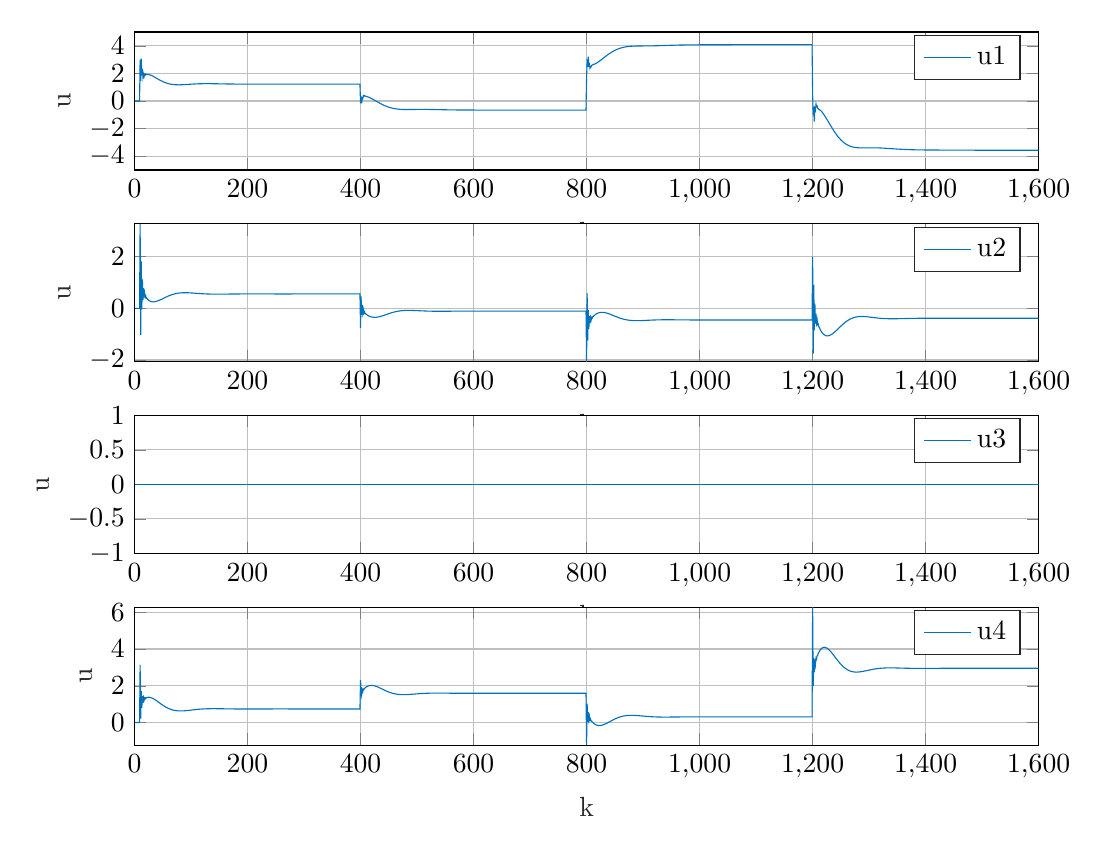
\begin{tikzpicture}

\begin{axis}[%
width=4.521in,
height=0.69in,
at={(0.758in,3.357in)},
scale only axis,
xmin=0,
xmax=1600,
xlabel style={font=\color{white!15!black}},
xlabel={k},
ymin=-5,
ymax=5,
ylabel style={font=\color{white!15!black}},
ylabel={u},
axis background/.style={fill=white},
xmajorgrids,
ymajorgrids,
legend style={legend cell align=left, align=left, draw=white!15!black}
]
\addplot [color=mycolor1]
  table[row sep=crcr]{%
1	0\\
2	0\\
3	0\\
4	0\\
5	0\\
6	0\\
7	0\\
8	0\\
9	0\\
10	2.9925\\
11	1.4423\\
12	3.0753\\
13	1.839\\
14	2.3231\\
15	1.7082\\
16	1.9443\\
17	1.759\\
18	1.9186\\
19	1.8739\\
20	1.9466\\
21	1.9208\\
22	1.9404\\
23	1.9213\\
24	1.9239\\
25	1.9116\\
26	1.9077\\
27	1.8958\\
28	1.8853\\
29	1.8695\\
30	1.8531\\
31	1.8338\\
32	1.8136\\
33	1.7919\\
34	1.7697\\
35	1.7465\\
36	1.723\\
37	1.699\\
38	1.6749\\
39	1.6507\\
40	1.6266\\
41	1.6027\\
42	1.5791\\
43	1.5558\\
44	1.5329\\
45	1.5106\\
46	1.4889\\
47	1.4677\\
48	1.4472\\
49	1.4274\\
50	1.4083\\
51	1.39\\
52	1.3724\\
53	1.3556\\
54	1.3396\\
55	1.3244\\
56	1.31\\
57	1.2964\\
58	1.2836\\
59	1.2717\\
60	1.2605\\
61	1.25\\
62	1.2404\\
63	1.2315\\
64	1.2234\\
65	1.2159\\
66	1.2092\\
67	1.2031\\
68	1.1977\\
69	1.1929\\
70	1.1888\\
71	1.1852\\
72	1.1822\\
73	1.1797\\
74	1.1777\\
75	1.1762\\
76	1.1751\\
77	1.1744\\
78	1.1742\\
79	1.1743\\
80	1.1747\\
81	1.1755\\
82	1.1765\\
83	1.1779\\
84	1.1794\\
85	1.1812\\
86	1.1831\\
87	1.1853\\
88	1.1875\\
89	1.1899\\
90	1.1925\\
91	1.1951\\
92	1.1977\\
93	1.2004\\
94	1.2032\\
95	1.206\\
96	1.2088\\
97	1.2115\\
98	1.2143\\
99	1.217\\
100	1.2197\\
101	1.2223\\
102	1.2249\\
103	1.2274\\
104	1.2298\\
105	1.2322\\
106	1.2344\\
107	1.2366\\
108	1.2387\\
109	1.2406\\
110	1.2425\\
111	1.2442\\
112	1.2458\\
113	1.2474\\
114	1.2488\\
115	1.2501\\
116	1.2513\\
117	1.2524\\
118	1.2533\\
119	1.2542\\
120	1.2549\\
121	1.2556\\
122	1.2562\\
123	1.2566\\
124	1.257\\
125	1.2572\\
126	1.2574\\
127	1.2575\\
128	1.2575\\
129	1.2575\\
130	1.2574\\
131	1.2571\\
132	1.2569\\
133	1.2565\\
134	1.2562\\
135	1.2557\\
136	1.2552\\
137	1.2547\\
138	1.2541\\
139	1.2535\\
140	1.2529\\
141	1.2522\\
142	1.2515\\
143	1.2508\\
144	1.25\\
145	1.2492\\
146	1.2485\\
147	1.2477\\
148	1.2469\\
149	1.2461\\
150	1.2453\\
151	1.2445\\
152	1.2437\\
153	1.2429\\
154	1.2421\\
155	1.2413\\
156	1.2406\\
157	1.2398\\
158	1.2391\\
159	1.2384\\
160	1.2377\\
161	1.237\\
162	1.2363\\
163	1.2357\\
164	1.235\\
165	1.2344\\
166	1.2338\\
167	1.2333\\
168	1.2327\\
169	1.2322\\
170	1.2317\\
171	1.2312\\
172	1.2308\\
173	1.2303\\
174	1.2299\\
175	1.2295\\
176	1.2292\\
177	1.2288\\
178	1.2285\\
179	1.2282\\
180	1.2279\\
181	1.2276\\
182	1.2274\\
183	1.2271\\
184	1.2269\\
185	1.2267\\
186	1.2266\\
187	1.2264\\
188	1.2263\\
189	1.2261\\
190	1.226\\
191	1.2259\\
192	1.2258\\
193	1.2257\\
194	1.2256\\
195	1.2256\\
196	1.2255\\
197	1.2255\\
198	1.2254\\
199	1.2254\\
200	1.2254\\
201	1.2254\\
202	1.2253\\
203	1.2253\\
204	1.2253\\
205	1.2253\\
206	1.2253\\
207	1.2253\\
208	1.2254\\
209	1.2254\\
210	1.2254\\
211	1.2254\\
212	1.2254\\
213	1.2254\\
214	1.2254\\
215	1.2255\\
216	1.2255\\
217	1.2255\\
218	1.2255\\
219	1.2255\\
220	1.2256\\
221	1.2256\\
222	1.2256\\
223	1.2256\\
224	1.2256\\
225	1.2256\\
226	1.2256\\
227	1.2256\\
228	1.2256\\
229	1.2256\\
230	1.2256\\
231	1.2256\\
232	1.2256\\
233	1.2256\\
234	1.2256\\
235	1.2256\\
236	1.2256\\
237	1.2256\\
238	1.2255\\
239	1.2255\\
240	1.2255\\
241	1.2255\\
242	1.2255\\
243	1.2254\\
244	1.2254\\
245	1.2254\\
246	1.2254\\
247	1.2253\\
248	1.2253\\
249	1.2253\\
250	1.2252\\
251	1.2252\\
252	1.2252\\
253	1.2251\\
254	1.2251\\
255	1.2251\\
256	1.225\\
257	1.225\\
258	1.225\\
259	1.2249\\
260	1.2249\\
261	1.2249\\
262	1.2248\\
263	1.2248\\
264	1.2248\\
265	1.2247\\
266	1.2247\\
267	1.2247\\
268	1.2246\\
269	1.2246\\
270	1.2246\\
271	1.2245\\
272	1.2245\\
273	1.2245\\
274	1.2244\\
275	1.2244\\
276	1.2244\\
277	1.2244\\
278	1.2243\\
279	1.2243\\
280	1.2243\\
281	1.2243\\
282	1.2242\\
283	1.2242\\
284	1.2242\\
285	1.2242\\
286	1.2241\\
287	1.2241\\
288	1.2241\\
289	1.2241\\
290	1.2241\\
291	1.2241\\
292	1.224\\
293	1.224\\
294	1.224\\
295	1.224\\
296	1.224\\
297	1.224\\
298	1.224\\
299	1.2239\\
300	1.2239\\
301	1.2239\\
302	1.2239\\
303	1.2239\\
304	1.2239\\
305	1.2239\\
306	1.2239\\
307	1.2239\\
308	1.2239\\
309	1.2238\\
310	1.2238\\
311	1.2238\\
312	1.2238\\
313	1.2238\\
314	1.2238\\
315	1.2238\\
316	1.2238\\
317	1.2238\\
318	1.2238\\
319	1.2238\\
320	1.2238\\
321	1.2238\\
322	1.2238\\
323	1.2238\\
324	1.2238\\
325	1.2238\\
326	1.2238\\
327	1.2238\\
328	1.2238\\
329	1.2237\\
330	1.2237\\
331	1.2237\\
332	1.2237\\
333	1.2237\\
334	1.2237\\
335	1.2237\\
336	1.2237\\
337	1.2237\\
338	1.2237\\
339	1.2237\\
340	1.2237\\
341	1.2237\\
342	1.2237\\
343	1.2237\\
344	1.2237\\
345	1.2237\\
346	1.2237\\
347	1.2237\\
348	1.2237\\
349	1.2237\\
350	1.2237\\
351	1.2237\\
352	1.2237\\
353	1.2237\\
354	1.2237\\
355	1.2237\\
356	1.2237\\
357	1.2237\\
358	1.2237\\
359	1.2237\\
360	1.2237\\
361	1.2237\\
362	1.2237\\
363	1.2237\\
364	1.2237\\
365	1.2237\\
366	1.2237\\
367	1.2237\\
368	1.2236\\
369	1.2236\\
370	1.2236\\
371	1.2236\\
372	1.2236\\
373	1.2236\\
374	1.2236\\
375	1.2236\\
376	1.2236\\
377	1.2236\\
378	1.2236\\
379	1.2236\\
380	1.2236\\
381	1.2236\\
382	1.2236\\
383	1.2236\\
384	1.2236\\
385	1.2236\\
386	1.2236\\
387	1.2236\\
388	1.2236\\
389	1.2236\\
390	1.2236\\
391	1.2236\\
392	1.2236\\
393	1.2236\\
394	1.2236\\
395	1.2236\\
396	1.2236\\
397	1.2236\\
398	1.2236\\
399	1.2236\\
400	-0.17291\\
401	0.33545\\
402	-0.16013\\
403	0.22667\\
404	0.18382\\
405	0.38482\\
406	0.35389\\
407	0.39963\\
408	0.35408\\
409	0.35374\\
410	0.32695\\
411	0.32386\\
412	0.30929\\
413	0.30143\\
414	0.28557\\
415	0.27034\\
416	0.25084\\
417	0.23144\\
418	0.2104\\
419	0.18946\\
420	0.16775\\
421	0.14589\\
422	0.12347\\
423	0.10077\\
424	0.077693\\
425	0.054428\\
426	0.030984\\
427	0.0074766\\
428	-0.016059\\
429	-0.039549\\
430	-0.062952\\
431	-0.08621\\
432	-0.10928\\
433	-0.1321\\
434	-0.15463\\
435	-0.17683\\
436	-0.19864\\
437	-0.22004\\
438	-0.24099\\
439	-0.26145\\
440	-0.28139\\
441	-0.3008\\
442	-0.31963\\
443	-0.33789\\
444	-0.35554\\
445	-0.37257\\
446	-0.38897\\
447	-0.40474\\
448	-0.41986\\
449	-0.43434\\
450	-0.44817\\
451	-0.46135\\
452	-0.47389\\
453	-0.48579\\
454	-0.49706\\
455	-0.50771\\
456	-0.51775\\
457	-0.52718\\
458	-0.53603\\
459	-0.5443\\
460	-0.55202\\
461	-0.55919\\
462	-0.56584\\
463	-0.57199\\
464	-0.57764\\
465	-0.58283\\
466	-0.58756\\
467	-0.59186\\
468	-0.59576\\
469	-0.59926\\
470	-0.60239\\
471	-0.60516\\
472	-0.60761\\
473	-0.60975\\
474	-0.61159\\
475	-0.61316\\
476	-0.61448\\
477	-0.61556\\
478	-0.61642\\
479	-0.61708\\
480	-0.61756\\
481	-0.61788\\
482	-0.61804\\
483	-0.61807\\
484	-0.61798\\
485	-0.61778\\
486	-0.61749\\
487	-0.61712\\
488	-0.61669\\
489	-0.6162\\
490	-0.61566\\
491	-0.6151\\
492	-0.6145\\
493	-0.6139\\
494	-0.61329\\
495	-0.61267\\
496	-0.61207\\
497	-0.61149\\
498	-0.61092\\
499	-0.61038\\
500	-0.60987\\
501	-0.6094\\
502	-0.60897\\
503	-0.60858\\
504	-0.60824\\
505	-0.60795\\
506	-0.60771\\
507	-0.60752\\
508	-0.60738\\
509	-0.6073\\
510	-0.60728\\
511	-0.60731\\
512	-0.60739\\
513	-0.60753\\
514	-0.60772\\
515	-0.60796\\
516	-0.60826\\
517	-0.60861\\
518	-0.609\\
519	-0.60945\\
520	-0.60993\\
521	-0.61047\\
522	-0.61104\\
523	-0.61165\\
524	-0.6123\\
525	-0.61299\\
526	-0.6137\\
527	-0.61445\\
528	-0.61522\\
529	-0.61602\\
530	-0.61685\\
531	-0.61769\\
532	-0.61855\\
533	-0.61942\\
534	-0.62031\\
535	-0.62122\\
536	-0.62213\\
537	-0.62304\\
538	-0.62396\\
539	-0.62489\\
540	-0.62581\\
541	-0.62674\\
542	-0.62766\\
543	-0.62857\\
544	-0.62948\\
545	-0.63038\\
546	-0.63128\\
547	-0.63216\\
548	-0.63303\\
549	-0.63389\\
550	-0.63473\\
551	-0.63556\\
552	-0.63637\\
553	-0.63717\\
554	-0.63795\\
555	-0.63871\\
556	-0.63945\\
557	-0.64018\\
558	-0.64088\\
559	-0.64156\\
560	-0.64223\\
561	-0.64287\\
562	-0.6435\\
563	-0.6441\\
564	-0.64468\\
565	-0.64525\\
566	-0.64579\\
567	-0.64631\\
568	-0.64681\\
569	-0.6473\\
570	-0.64776\\
571	-0.6482\\
572	-0.64863\\
573	-0.64904\\
574	-0.64943\\
575	-0.6498\\
576	-0.65016\\
577	-0.6505\\
578	-0.65082\\
579	-0.65113\\
580	-0.65142\\
581	-0.6517\\
582	-0.65196\\
583	-0.65221\\
584	-0.65245\\
585	-0.65268\\
586	-0.65289\\
587	-0.65309\\
588	-0.65329\\
589	-0.65347\\
590	-0.65364\\
591	-0.65381\\
592	-0.65396\\
593	-0.65411\\
594	-0.65425\\
595	-0.65438\\
596	-0.65451\\
597	-0.65463\\
598	-0.65474\\
599	-0.65485\\
600	-0.65495\\
601	-0.65505\\
602	-0.65515\\
603	-0.65524\\
604	-0.65532\\
605	-0.65541\\
606	-0.65549\\
607	-0.65557\\
608	-0.65564\\
609	-0.65572\\
610	-0.65579\\
611	-0.65586\\
612	-0.65593\\
613	-0.65599\\
614	-0.65606\\
615	-0.65612\\
616	-0.65619\\
617	-0.65625\\
618	-0.65632\\
619	-0.65638\\
620	-0.65644\\
621	-0.6565\\
622	-0.65656\\
623	-0.65662\\
624	-0.65669\\
625	-0.65675\\
626	-0.65681\\
627	-0.65687\\
628	-0.65693\\
629	-0.65699\\
630	-0.65705\\
631	-0.65711\\
632	-0.65717\\
633	-0.65724\\
634	-0.6573\\
635	-0.65736\\
636	-0.65742\\
637	-0.65748\\
638	-0.65754\\
639	-0.6576\\
640	-0.65766\\
641	-0.65772\\
642	-0.65778\\
643	-0.65784\\
644	-0.6579\\
645	-0.65796\\
646	-0.65802\\
647	-0.65808\\
648	-0.65814\\
649	-0.6582\\
650	-0.65825\\
651	-0.65831\\
652	-0.65837\\
653	-0.65842\\
654	-0.65848\\
655	-0.65853\\
656	-0.65859\\
657	-0.65864\\
658	-0.65869\\
659	-0.65874\\
660	-0.65879\\
661	-0.65884\\
662	-0.65889\\
663	-0.65894\\
664	-0.65898\\
665	-0.65903\\
666	-0.65908\\
667	-0.65912\\
668	-0.65916\\
669	-0.65921\\
670	-0.65925\\
671	-0.65929\\
672	-0.65933\\
673	-0.65937\\
674	-0.6594\\
675	-0.65944\\
676	-0.65948\\
677	-0.65951\\
678	-0.65954\\
679	-0.65958\\
680	-0.65961\\
681	-0.65964\\
682	-0.65967\\
683	-0.6597\\
684	-0.65973\\
685	-0.65976\\
686	-0.65978\\
687	-0.65981\\
688	-0.65983\\
689	-0.65986\\
690	-0.65988\\
691	-0.65991\\
692	-0.65993\\
693	-0.65995\\
694	-0.65997\\
695	-0.65999\\
696	-0.66001\\
697	-0.66003\\
698	-0.66005\\
699	-0.66007\\
700	-0.66009\\
701	-0.6601\\
702	-0.66012\\
703	-0.66013\\
704	-0.66015\\
705	-0.66016\\
706	-0.66018\\
707	-0.66019\\
708	-0.66021\\
709	-0.66022\\
710	-0.66023\\
711	-0.66024\\
712	-0.66026\\
713	-0.66027\\
714	-0.66028\\
715	-0.66029\\
716	-0.6603\\
717	-0.66031\\
718	-0.66032\\
719	-0.66033\\
720	-0.66034\\
721	-0.66035\\
722	-0.66036\\
723	-0.66037\\
724	-0.66038\\
725	-0.66039\\
726	-0.6604\\
727	-0.6604\\
728	-0.66041\\
729	-0.66042\\
730	-0.66043\\
731	-0.66043\\
732	-0.66044\\
733	-0.66045\\
734	-0.66046\\
735	-0.66046\\
736	-0.66047\\
737	-0.66048\\
738	-0.66048\\
739	-0.66049\\
740	-0.6605\\
741	-0.6605\\
742	-0.66051\\
743	-0.66052\\
744	-0.66052\\
745	-0.66053\\
746	-0.66053\\
747	-0.66054\\
748	-0.66054\\
749	-0.66055\\
750	-0.66056\\
751	-0.66056\\
752	-0.66057\\
753	-0.66057\\
754	-0.66058\\
755	-0.66058\\
756	-0.66059\\
757	-0.66059\\
758	-0.6606\\
759	-0.6606\\
760	-0.6606\\
761	-0.66061\\
762	-0.66061\\
763	-0.66062\\
764	-0.66062\\
765	-0.66063\\
766	-0.66063\\
767	-0.66063\\
768	-0.66064\\
769	-0.66064\\
770	-0.66065\\
771	-0.66065\\
772	-0.66065\\
773	-0.66066\\
774	-0.66066\\
775	-0.66066\\
776	-0.66067\\
777	-0.66067\\
778	-0.66067\\
779	-0.66068\\
780	-0.66068\\
781	-0.66068\\
782	-0.66069\\
783	-0.66069\\
784	-0.66069\\
785	-0.6607\\
786	-0.6607\\
787	-0.6607\\
788	-0.6607\\
789	-0.66071\\
790	-0.66071\\
791	-0.66071\\
792	-0.66071\\
793	-0.66072\\
794	-0.66072\\
795	-0.66072\\
796	-0.66072\\
797	-0.66073\\
798	-0.66073\\
799	-0.66073\\
800	1.7333\\
801	2.8496\\
802	2.6978\\
803	3.2179\\
804	2.5769\\
805	2.6552\\
806	2.3768\\
807	2.5013\\
808	2.4782\\
809	2.5892\\
810	2.6013\\
811	2.6468\\
812	2.6455\\
813	2.6629\\
814	2.6688\\
815	2.6888\\
816	2.7074\\
817	2.7326\\
818	2.7571\\
819	2.784\\
820	2.8106\\
821	2.8386\\
822	2.867\\
823	2.8966\\
824	2.9268\\
825	2.9578\\
826	2.9891\\
827	3.0209\\
828	3.0528\\
829	3.0848\\
830	3.1168\\
831	3.1488\\
832	3.1806\\
833	3.2122\\
834	3.2435\\
835	3.2744\\
836	3.3049\\
837	3.3349\\
838	3.3645\\
839	3.3934\\
840	3.4218\\
841	3.4495\\
842	3.4766\\
843	3.503\\
844	3.5286\\
845	3.5535\\
846	3.5777\\
847	3.6011\\
848	3.6236\\
849	3.6454\\
850	3.6664\\
851	3.6866\\
852	3.706\\
853	3.7245\\
854	3.7423\\
855	3.7593\\
856	3.7754\\
857	3.7908\\
858	3.8055\\
859	3.8193\\
860	3.8325\\
861	3.8449\\
862	3.8566\\
863	3.8676\\
864	3.878\\
865	3.8877\\
866	3.8968\\
867	3.9053\\
868	3.9132\\
869	3.9205\\
870	3.9274\\
871	3.9337\\
872	3.9395\\
873	3.9448\\
874	3.9497\\
875	3.9542\\
876	3.9583\\
877	3.9621\\
878	3.9655\\
879	3.9685\\
880	3.9713\\
881	3.9737\\
882	3.9759\\
883	3.9779\\
884	3.9797\\
885	3.9812\\
886	3.9825\\
887	3.9837\\
888	3.9848\\
889	3.9857\\
890	3.9864\\
891	3.9871\\
892	3.9877\\
893	3.9882\\
894	3.9886\\
895	3.989\\
896	3.9894\\
897	3.9897\\
898	3.9899\\
899	3.9902\\
900	3.9905\\
901	3.9907\\
902	3.991\\
903	3.9913\\
904	3.9916\\
905	3.9919\\
906	3.9923\\
907	3.9927\\
908	3.9931\\
909	3.9935\\
910	3.994\\
911	3.9946\\
912	3.9952\\
913	3.9958\\
914	3.9965\\
915	3.9972\\
916	3.998\\
917	3.9988\\
918	3.9997\\
919	4.0006\\
920	4.0015\\
921	4.0025\\
922	4.0035\\
923	4.0046\\
924	4.0057\\
925	4.0069\\
926	4.008\\
927	4.0092\\
928	4.0105\\
929	4.0117\\
930	4.013\\
931	4.0143\\
932	4.0156\\
933	4.017\\
934	4.0183\\
935	4.0197\\
936	4.021\\
937	4.0224\\
938	4.0238\\
939	4.0252\\
940	4.0266\\
941	4.0279\\
942	4.0293\\
943	4.0307\\
944	4.032\\
945	4.0334\\
946	4.0347\\
947	4.036\\
948	4.0374\\
949	4.0386\\
950	4.0399\\
951	4.0412\\
952	4.0424\\
953	4.0436\\
954	4.0448\\
955	4.046\\
956	4.0471\\
957	4.0482\\
958	4.0493\\
959	4.0504\\
960	4.0514\\
961	4.0524\\
962	4.0534\\
963	4.0544\\
964	4.0553\\
965	4.0562\\
966	4.0571\\
967	4.0579\\
968	4.0588\\
969	4.0596\\
970	4.0603\\
971	4.0611\\
972	4.0618\\
973	4.0625\\
974	4.0632\\
975	4.0638\\
976	4.0644\\
977	4.065\\
978	4.0656\\
979	4.0661\\
980	4.0667\\
981	4.0672\\
982	4.0676\\
983	4.0681\\
984	4.0686\\
985	4.069\\
986	4.0694\\
987	4.0698\\
988	4.0702\\
989	4.0705\\
990	4.0709\\
991	4.0712\\
992	4.0715\\
993	4.0718\\
994	4.0721\\
995	4.0724\\
996	4.0727\\
997	4.0729\\
998	4.0732\\
999	4.0734\\
1000	4.0736\\
1001	4.0738\\
1002	4.0741\\
1003	4.0743\\
1004	4.0745\\
1005	4.0746\\
1006	4.0748\\
1007	4.075\\
1008	4.0752\\
1009	4.0753\\
1010	4.0755\\
1011	4.0757\\
1012	4.0758\\
1013	4.076\\
1014	4.0761\\
1015	4.0763\\
1016	4.0764\\
1017	4.0765\\
1018	4.0767\\
1019	4.0768\\
1020	4.0769\\
1021	4.0771\\
1022	4.0772\\
1023	4.0773\\
1024	4.0774\\
1025	4.0776\\
1026	4.0777\\
1027	4.0778\\
1028	4.0779\\
1029	4.078\\
1030	4.0781\\
1031	4.0783\\
1032	4.0784\\
1033	4.0785\\
1034	4.0786\\
1035	4.0787\\
1036	4.0788\\
1037	4.0789\\
1038	4.079\\
1039	4.0791\\
1040	4.0792\\
1041	4.0793\\
1042	4.0795\\
1043	4.0796\\
1044	4.0797\\
1045	4.0798\\
1046	4.0799\\
1047	4.08\\
1048	4.0801\\
1049	4.0802\\
1050	4.0802\\
1051	4.0803\\
1052	4.0804\\
1053	4.0805\\
1054	4.0806\\
1055	4.0807\\
1056	4.0808\\
1057	4.0809\\
1058	4.081\\
1059	4.0811\\
1060	4.0811\\
1061	4.0812\\
1062	4.0813\\
1063	4.0814\\
1064	4.0815\\
1065	4.0815\\
1066	4.0816\\
1067	4.0817\\
1068	4.0818\\
1069	4.0818\\
1070	4.0819\\
1071	4.082\\
1072	4.082\\
1073	4.0821\\
1074	4.0822\\
1075	4.0822\\
1076	4.0823\\
1077	4.0823\\
1078	4.0824\\
1079	4.0825\\
1080	4.0825\\
1081	4.0826\\
1082	4.0826\\
1083	4.0827\\
1084	4.0827\\
1085	4.0828\\
1086	4.0828\\
1087	4.0829\\
1088	4.0829\\
1089	4.0829\\
1090	4.083\\
1091	4.083\\
1092	4.0831\\
1093	4.0831\\
1094	4.0831\\
1095	4.0832\\
1096	4.0832\\
1097	4.0832\\
1098	4.0833\\
1099	4.0833\\
1100	4.0833\\
1101	4.0834\\
1102	4.0834\\
1103	4.0834\\
1104	4.0835\\
1105	4.0835\\
1106	4.0835\\
1107	4.0835\\
1108	4.0836\\
1109	4.0836\\
1110	4.0836\\
1111	4.0836\\
1112	4.0837\\
1113	4.0837\\
1114	4.0837\\
1115	4.0837\\
1116	4.0837\\
1117	4.0838\\
1118	4.0838\\
1119	4.0838\\
1120	4.0838\\
1121	4.0838\\
1122	4.0839\\
1123	4.0839\\
1124	4.0839\\
1125	4.0839\\
1126	4.0839\\
1127	4.0839\\
1128	4.0839\\
1129	4.084\\
1130	4.084\\
1131	4.084\\
1132	4.084\\
1133	4.084\\
1134	4.084\\
1135	4.084\\
1136	4.0841\\
1137	4.0841\\
1138	4.0841\\
1139	4.0841\\
1140	4.0841\\
1141	4.0841\\
1142	4.0841\\
1143	4.0841\\
1144	4.0841\\
1145	4.0842\\
1146	4.0842\\
1147	4.0842\\
1148	4.0842\\
1149	4.0842\\
1150	4.0842\\
1151	4.0842\\
1152	4.0842\\
1153	4.0842\\
1154	4.0842\\
1155	4.0843\\
1156	4.0843\\
1157	4.0843\\
1158	4.0843\\
1159	4.0843\\
1160	4.0843\\
1161	4.0843\\
1162	4.0843\\
1163	4.0843\\
1164	4.0843\\
1165	4.0843\\
1166	4.0843\\
1167	4.0843\\
1168	4.0844\\
1169	4.0844\\
1170	4.0844\\
1171	4.0844\\
1172	4.0844\\
1173	4.0844\\
1174	4.0844\\
1175	4.0844\\
1176	4.0844\\
1177	4.0844\\
1178	4.0844\\
1179	4.0844\\
1180	4.0844\\
1181	4.0844\\
1182	4.0844\\
1183	4.0844\\
1184	4.0844\\
1185	4.0845\\
1186	4.0845\\
1187	4.0845\\
1188	4.0845\\
1189	4.0845\\
1190	4.0845\\
1191	4.0845\\
1192	4.0845\\
1193	4.0845\\
1194	4.0845\\
1195	4.0845\\
1196	4.0845\\
1197	4.0845\\
1198	4.0845\\
1199	4.0845\\
1200	0.49352\\
1201	-1.0135\\
1202	-0.77921\\
1203	-1.4955\\
1204	-0.53316\\
1205	-0.63817\\
1206	-0.22358\\
1207	-0.40404\\
1208	-0.36755\\
1209	-0.53007\\
1210	-0.54904\\
1211	-0.62006\\
1212	-0.62517\\
1213	-0.66034\\
1214	-0.68076\\
1215	-0.72366\\
1216	-0.76592\\
1217	-0.81937\\
1218	-0.87271\\
1219	-0.93065\\
1220	-0.98897\\
1221	-1.0501\\
1222	-1.1125\\
1223	-1.1772\\
1224	-1.2431\\
1225	-1.3105\\
1226	-1.3786\\
1227	-1.4475\\
1228	-1.5166\\
1229	-1.5859\\
1230	-1.655\\
1231	-1.7239\\
1232	-1.7924\\
1233	-1.8602\\
1234	-1.9273\\
1235	-1.9935\\
1236	-2.0587\\
1237	-2.1227\\
1238	-2.1855\\
1239	-2.247\\
1240	-2.307\\
1241	-2.3655\\
1242	-2.4224\\
1243	-2.4777\\
1244	-2.5313\\
1245	-2.5832\\
1246	-2.6333\\
1247	-2.6816\\
1248	-2.7281\\
1249	-2.7728\\
1250	-2.8156\\
1251	-2.8566\\
1252	-2.8958\\
1253	-2.9331\\
1254	-2.9687\\
1255	-3.0024\\
1256	-3.0344\\
1257	-3.0647\\
1258	-3.0933\\
1259	-3.1202\\
1260	-3.1455\\
1261	-3.1692\\
1262	-3.1913\\
1263	-3.212\\
1264	-3.2312\\
1265	-3.2491\\
1266	-3.2656\\
1267	-3.2808\\
1268	-3.2948\\
1269	-3.3076\\
1270	-3.3193\\
1271	-3.3299\\
1272	-3.3395\\
1273	-3.3482\\
1274	-3.3559\\
1275	-3.3628\\
1276	-3.369\\
1277	-3.3743\\
1278	-3.379\\
1279	-3.3831\\
1280	-3.3865\\
1281	-3.3894\\
1282	-3.3918\\
1283	-3.3938\\
1284	-3.3953\\
1285	-3.3965\\
1286	-3.3973\\
1287	-3.3979\\
1288	-3.3982\\
1289	-3.3982\\
1290	-3.3981\\
1291	-3.3979\\
1292	-3.3975\\
1293	-3.397\\
1294	-3.3964\\
1295	-3.3958\\
1296	-3.3952\\
1297	-3.3945\\
1298	-3.3939\\
1299	-3.3933\\
1300	-3.3927\\
1301	-3.3922\\
1302	-3.3918\\
1303	-3.3914\\
1304	-3.3912\\
1305	-3.391\\
1306	-3.391\\
1307	-3.3911\\
1308	-3.3913\\
1309	-3.3916\\
1310	-3.392\\
1311	-3.3926\\
1312	-3.3933\\
1313	-3.3942\\
1314	-3.3952\\
1315	-3.3963\\
1316	-3.3975\\
1317	-3.3989\\
1318	-3.4004\\
1319	-3.402\\
1320	-3.4037\\
1321	-3.4055\\
1322	-3.4075\\
1323	-3.4095\\
1324	-3.4117\\
1325	-3.4139\\
1326	-3.4162\\
1327	-3.4186\\
1328	-3.421\\
1329	-3.4236\\
1330	-3.4262\\
1331	-3.4288\\
1332	-3.4315\\
1333	-3.4342\\
1334	-3.437\\
1335	-3.4398\\
1336	-3.4426\\
1337	-3.4454\\
1338	-3.4483\\
1339	-3.4511\\
1340	-3.4539\\
1341	-3.4568\\
1342	-3.4596\\
1343	-3.4624\\
1344	-3.4652\\
1345	-3.468\\
1346	-3.4708\\
1347	-3.4735\\
1348	-3.4762\\
1349	-3.4788\\
1350	-3.4815\\
1351	-3.484\\
1352	-3.4865\\
1353	-3.489\\
1354	-3.4914\\
1355	-3.4938\\
1356	-3.4961\\
1357	-3.4984\\
1358	-3.5006\\
1359	-3.5027\\
1360	-3.5048\\
1361	-3.5069\\
1362	-3.5088\\
1363	-3.5107\\
1364	-3.5126\\
1365	-3.5144\\
1366	-3.5161\\
1367	-3.5178\\
1368	-3.5194\\
1369	-3.521\\
1370	-3.5225\\
1371	-3.5239\\
1372	-3.5253\\
1373	-3.5266\\
1374	-3.5279\\
1375	-3.5292\\
1376	-3.5303\\
1377	-3.5315\\
1378	-3.5325\\
1379	-3.5336\\
1380	-3.5346\\
1381	-3.5355\\
1382	-3.5364\\
1383	-3.5373\\
1384	-3.5381\\
1385	-3.5389\\
1386	-3.5396\\
1387	-3.5403\\
1388	-3.541\\
1389	-3.5417\\
1390	-3.5423\\
1391	-3.5429\\
1392	-3.5434\\
1393	-3.544\\
1394	-3.5445\\
1395	-3.545\\
1396	-3.5454\\
1397	-3.5459\\
1398	-3.5463\\
1399	-3.5467\\
1400	-3.5471\\
1401	-3.5475\\
1402	-3.5478\\
1403	-3.5482\\
1404	-3.5485\\
1405	-3.5488\\
1406	-3.5491\\
1407	-3.5494\\
1408	-3.5497\\
1409	-3.55\\
1410	-3.5503\\
1411	-3.5505\\
1412	-3.5508\\
1413	-3.5511\\
1414	-3.5513\\
1415	-3.5516\\
1416	-3.5518\\
1417	-3.552\\
1418	-3.5523\\
1419	-3.5525\\
1420	-3.5527\\
1421	-3.5529\\
1422	-3.5532\\
1423	-3.5534\\
1424	-3.5536\\
1425	-3.5538\\
1426	-3.554\\
1427	-3.5543\\
1428	-3.5545\\
1429	-3.5547\\
1430	-3.5549\\
1431	-3.5551\\
1432	-3.5553\\
1433	-3.5555\\
1434	-3.5557\\
1435	-3.5559\\
1436	-3.5562\\
1437	-3.5564\\
1438	-3.5566\\
1439	-3.5568\\
1440	-3.557\\
1441	-3.5572\\
1442	-3.5574\\
1443	-3.5576\\
1444	-3.5578\\
1445	-3.558\\
1446	-3.5582\\
1447	-3.5583\\
1448	-3.5585\\
1449	-3.5587\\
1450	-3.5589\\
1451	-3.5591\\
1452	-3.5593\\
1453	-3.5595\\
1454	-3.5596\\
1455	-3.5598\\
1456	-3.56\\
1457	-3.5602\\
1458	-3.5603\\
1459	-3.5605\\
1460	-3.5607\\
1461	-3.5608\\
1462	-3.561\\
1463	-3.5611\\
1464	-3.5613\\
1465	-3.5614\\
1466	-3.5616\\
1467	-3.5617\\
1468	-3.5619\\
1469	-3.562\\
1470	-3.5621\\
1471	-3.5623\\
1472	-3.5624\\
1473	-3.5625\\
1474	-3.5626\\
1475	-3.5628\\
1476	-3.5629\\
1477	-3.563\\
1478	-3.5631\\
1479	-3.5632\\
1480	-3.5633\\
1481	-3.5634\\
1482	-3.5635\\
1483	-3.5636\\
1484	-3.5637\\
1485	-3.5638\\
1486	-3.5639\\
1487	-3.564\\
1488	-3.5641\\
1489	-3.5641\\
1490	-3.5642\\
1491	-3.5643\\
1492	-3.5644\\
1493	-3.5644\\
1494	-3.5645\\
1495	-3.5646\\
1496	-3.5646\\
1497	-3.5647\\
1498	-3.5648\\
1499	-3.5648\\
1500	-3.5649\\
1501	-3.5649\\
1502	-3.565\\
1503	-3.5651\\
1504	-3.5651\\
1505	-3.5652\\
1506	-3.5652\\
1507	-3.5653\\
1508	-3.5653\\
1509	-3.5654\\
1510	-3.5654\\
1511	-3.5654\\
1512	-3.5655\\
1513	-3.5655\\
1514	-3.5656\\
1515	-3.5656\\
1516	-3.5656\\
1517	-3.5657\\
1518	-3.5657\\
1519	-3.5657\\
1520	-3.5658\\
1521	-3.5658\\
1522	-3.5658\\
1523	-3.5659\\
1524	-3.5659\\
1525	-3.5659\\
1526	-3.566\\
1527	-3.566\\
1528	-3.566\\
1529	-3.566\\
1530	-3.5661\\
1531	-3.5661\\
1532	-3.5661\\
1533	-3.5661\\
1534	-3.5662\\
1535	-3.5662\\
1536	-3.5662\\
1537	-3.5662\\
1538	-3.5663\\
1539	-3.5663\\
1540	-3.5663\\
1541	-3.5663\\
1542	-3.5663\\
1543	-3.5664\\
1544	-3.5664\\
1545	-3.5664\\
1546	-3.5664\\
1547	-3.5664\\
1548	-3.5665\\
1549	-3.5665\\
1550	-3.5665\\
1551	-3.5665\\
1552	-3.5665\\
1553	-3.5666\\
1554	-3.5666\\
1555	-3.5666\\
1556	-3.5666\\
1557	-3.5666\\
1558	-3.5666\\
1559	-3.5667\\
1560	-3.5667\\
1561	-3.5667\\
1562	-3.5667\\
1563	-3.5667\\
1564	-3.5667\\
1565	-3.5667\\
1566	-3.5668\\
1567	-3.5668\\
1568	-3.5668\\
1569	-3.5668\\
1570	-3.5668\\
1571	-3.5668\\
1572	-3.5668\\
1573	-3.5668\\
1574	-3.5669\\
1575	-3.5669\\
1576	-3.5669\\
1577	-3.5669\\
1578	-3.5669\\
1579	-3.5669\\
1580	-3.5669\\
1581	-3.5669\\
1582	-3.5669\\
1583	-3.567\\
1584	-3.567\\
1585	-3.567\\
1586	-3.567\\
1587	-3.567\\
1588	-3.567\\
1589	-3.567\\
1590	-3.567\\
1591	-3.567\\
1592	-3.567\\
1593	-3.567\\
1594	-3.567\\
1595	-3.5671\\
1596	-3.5671\\
1597	-3.5671\\
1598	-3.5671\\
1599	-3.5671\\
1600	-3.5671\\
};
\addlegendentry{u1}

\end{axis}

\begin{axis}[%
width=4.521in,
height=0.69in,
at={(0.758in,2.398in)},
scale only axis,
xmin=0,
xmax=1600,
xlabel style={font=\color{white!15!black}},
xlabel={k},
ymin=-2.0717,
ymax=3.2744,
ylabel style={font=\color{white!15!black}},
ylabel={u},
axis background/.style={fill=white},
xmajorgrids,
ymajorgrids,
legend style={legend cell align=left, align=left, draw=white!15!black}
]
\addplot [color=mycolor1]
  table[row sep=crcr]{%
1	0\\
2	0\\
3	0\\
4	0\\
5	0\\
6	0\\
7	0\\
8	0\\
9	0\\
10	3.2744\\
11	-1.0328\\
12	1.819\\
13	-0.038181\\
14	1.1191\\
15	0.32637\\
16	0.78167\\
17	0.42867\\
18	0.59434\\
19	0.42675\\
20	0.47654\\
21	0.39045\\
22	0.39672\\
23	0.3487\\
24	0.34086\\
25	0.31223\\
26	0.30189\\
27	0.28442\\
28	0.2759\\
29	0.26568\\
30	0.26029\\
31	0.25522\\
32	0.25306\\
33	0.25186\\
34	0.2526\\
35	0.2544\\
36	0.25761\\
37	0.26178\\
38	0.26702\\
39	0.27308\\
40	0.27995\\
41	0.2875\\
42	0.29566\\
43	0.30435\\
44	0.3135\\
45	0.32304\\
46	0.33291\\
47	0.34304\\
48	0.35337\\
49	0.36386\\
50	0.37445\\
51	0.38509\\
52	0.39574\\
53	0.40635\\
54	0.4169\\
55	0.42733\\
56	0.43761\\
57	0.44772\\
58	0.45762\\
59	0.4673\\
60	0.47671\\
61	0.48586\\
62	0.4947\\
63	0.50324\\
64	0.51145\\
65	0.51932\\
66	0.52685\\
67	0.53402\\
68	0.54084\\
69	0.54728\\
70	0.55336\\
71	0.55908\\
72	0.56442\\
73	0.5694\\
74	0.57402\\
75	0.57828\\
76	0.58219\\
77	0.58575\\
78	0.58898\\
79	0.59188\\
80	0.59446\\
81	0.59673\\
82	0.5987\\
83	0.60038\\
84	0.60179\\
85	0.60293\\
86	0.60382\\
87	0.60447\\
88	0.60489\\
89	0.6051\\
90	0.60511\\
91	0.60493\\
92	0.60457\\
93	0.60404\\
94	0.60337\\
95	0.60255\\
96	0.60161\\
97	0.60055\\
98	0.59938\\
99	0.59813\\
100	0.59679\\
101	0.59537\\
102	0.5939\\
103	0.59237\\
104	0.5908\\
105	0.5892\\
106	0.58757\\
107	0.58592\\
108	0.58426\\
109	0.5826\\
110	0.58094\\
111	0.5793\\
112	0.57766\\
113	0.57605\\
114	0.57447\\
115	0.57291\\
116	0.57139\\
117	0.56991\\
118	0.56847\\
119	0.56708\\
120	0.56573\\
121	0.56444\\
122	0.56319\\
123	0.562\\
124	0.56087\\
125	0.55979\\
126	0.55876\\
127	0.5578\\
128	0.55689\\
129	0.55604\\
130	0.55524\\
131	0.5545\\
132	0.55382\\
133	0.55319\\
134	0.55262\\
135	0.5521\\
136	0.55163\\
137	0.55121\\
138	0.55084\\
139	0.55052\\
140	0.55025\\
141	0.55001\\
142	0.54982\\
143	0.54967\\
144	0.54956\\
145	0.54949\\
146	0.54945\\
147	0.54944\\
148	0.54946\\
149	0.54951\\
150	0.54959\\
151	0.54969\\
152	0.54981\\
153	0.54996\\
154	0.55012\\
155	0.5503\\
156	0.5505\\
157	0.55071\\
158	0.55093\\
159	0.55116\\
160	0.55141\\
161	0.55165\\
162	0.55191\\
163	0.55217\\
164	0.55243\\
165	0.5527\\
166	0.55296\\
167	0.55323\\
168	0.5535\\
169	0.55376\\
170	0.55402\\
171	0.55428\\
172	0.55453\\
173	0.55478\\
174	0.55502\\
175	0.55526\\
176	0.55548\\
177	0.55571\\
178	0.55592\\
179	0.55613\\
180	0.55632\\
181	0.55651\\
182	0.55669\\
183	0.55686\\
184	0.55703\\
185	0.55718\\
186	0.55733\\
187	0.55746\\
188	0.55759\\
189	0.55771\\
190	0.55782\\
191	0.55792\\
192	0.55801\\
193	0.55809\\
194	0.55817\\
195	0.55824\\
196	0.5583\\
197	0.55835\\
198	0.5584\\
199	0.55844\\
200	0.55847\\
201	0.5585\\
202	0.55852\\
203	0.55854\\
204	0.55855\\
205	0.55855\\
206	0.55855\\
207	0.55855\\
208	0.55854\\
209	0.55853\\
210	0.55851\\
211	0.55849\\
212	0.55847\\
213	0.55845\\
214	0.55842\\
215	0.55839\\
216	0.55836\\
217	0.55833\\
218	0.5583\\
219	0.55826\\
220	0.55823\\
221	0.55819\\
222	0.55815\\
223	0.55812\\
224	0.55808\\
225	0.55804\\
226	0.558\\
227	0.55797\\
228	0.55793\\
229	0.5579\\
230	0.55786\\
231	0.55783\\
232	0.55779\\
233	0.55776\\
234	0.55773\\
235	0.5577\\
236	0.55767\\
237	0.55764\\
238	0.55761\\
239	0.55758\\
240	0.55756\\
241	0.55754\\
242	0.55751\\
243	0.55749\\
244	0.55747\\
245	0.55746\\
246	0.55744\\
247	0.55742\\
248	0.55741\\
249	0.5574\\
250	0.55739\\
251	0.55738\\
252	0.55737\\
253	0.55736\\
254	0.55735\\
255	0.55735\\
256	0.55734\\
257	0.55734\\
258	0.55733\\
259	0.55733\\
260	0.55733\\
261	0.55733\\
262	0.55733\\
263	0.55733\\
264	0.55733\\
265	0.55734\\
266	0.55734\\
267	0.55734\\
268	0.55735\\
269	0.55735\\
270	0.55736\\
271	0.55736\\
272	0.55737\\
273	0.55737\\
274	0.55738\\
275	0.55739\\
276	0.55739\\
277	0.5574\\
278	0.55741\\
279	0.55741\\
280	0.55742\\
281	0.55743\\
282	0.55743\\
283	0.55744\\
284	0.55745\\
285	0.55745\\
286	0.55746\\
287	0.55747\\
288	0.55747\\
289	0.55748\\
290	0.55749\\
291	0.55749\\
292	0.5575\\
293	0.5575\\
294	0.55751\\
295	0.55751\\
296	0.55752\\
297	0.55752\\
298	0.55753\\
299	0.55753\\
300	0.55754\\
301	0.55754\\
302	0.55754\\
303	0.55755\\
304	0.55755\\
305	0.55755\\
306	0.55756\\
307	0.55756\\
308	0.55756\\
309	0.55756\\
310	0.55757\\
311	0.55757\\
312	0.55757\\
313	0.55757\\
314	0.55757\\
315	0.55757\\
316	0.55757\\
317	0.55757\\
318	0.55758\\
319	0.55758\\
320	0.55758\\
321	0.55758\\
322	0.55758\\
323	0.55758\\
324	0.55758\\
325	0.55758\\
326	0.55758\\
327	0.55758\\
328	0.55758\\
329	0.55758\\
330	0.55757\\
331	0.55757\\
332	0.55757\\
333	0.55757\\
334	0.55757\\
335	0.55757\\
336	0.55757\\
337	0.55757\\
338	0.55757\\
339	0.55757\\
340	0.55757\\
341	0.55757\\
342	0.55757\\
343	0.55757\\
344	0.55757\\
345	0.55756\\
346	0.55756\\
347	0.55756\\
348	0.55756\\
349	0.55756\\
350	0.55756\\
351	0.55756\\
352	0.55756\\
353	0.55756\\
354	0.55756\\
355	0.55756\\
356	0.55756\\
357	0.55756\\
358	0.55756\\
359	0.55756\\
360	0.55756\\
361	0.55756\\
362	0.55756\\
363	0.55756\\
364	0.55756\\
365	0.55756\\
366	0.55756\\
367	0.55755\\
368	0.55755\\
369	0.55755\\
370	0.55755\\
371	0.55755\\
372	0.55755\\
373	0.55755\\
374	0.55755\\
375	0.55755\\
376	0.55755\\
377	0.55755\\
378	0.55755\\
379	0.55755\\
380	0.55756\\
381	0.55756\\
382	0.55756\\
383	0.55756\\
384	0.55756\\
385	0.55756\\
386	0.55756\\
387	0.55756\\
388	0.55756\\
389	0.55756\\
390	0.55756\\
391	0.55756\\
392	0.55756\\
393	0.55756\\
394	0.55756\\
395	0.55756\\
396	0.55756\\
397	0.55756\\
398	0.55756\\
399	0.55756\\
400	-0.75222\\
401	0.45828\\
402	-0.25054\\
403	0.13193\\
404	-0.18284\\
405	-0.040654\\
406	-0.1855\\
407	-0.1387\\
408	-0.2095\\
409	-0.19975\\
410	-0.23796\\
411	-0.24203\\
412	-0.26529\\
413	-0.27368\\
414	-0.28932\\
415	-0.29813\\
416	-0.30928\\
417	-0.31696\\
418	-0.32501\\
419	-0.33103\\
420	-0.33661\\
421	-0.34079\\
422	-0.34423\\
423	-0.34656\\
424	-0.34808\\
425	-0.34865\\
426	-0.34843\\
427	-0.34738\\
428	-0.34558\\
429	-0.34307\\
430	-0.3399\\
431	-0.33611\\
432	-0.33175\\
433	-0.32687\\
434	-0.32151\\
435	-0.31572\\
436	-0.30956\\
437	-0.30305\\
438	-0.29626\\
439	-0.28921\\
440	-0.28196\\
441	-0.27453\\
442	-0.26698\\
443	-0.25932\\
444	-0.25161\\
445	-0.24387\\
446	-0.23613\\
447	-0.22841\\
448	-0.22076\\
449	-0.21319\\
450	-0.20572\\
451	-0.19838\\
452	-0.19118\\
453	-0.18414\\
454	-0.17729\\
455	-0.17063\\
456	-0.16417\\
457	-0.15794\\
458	-0.15192\\
459	-0.14615\\
460	-0.14062\\
461	-0.13533\\
462	-0.1303\\
463	-0.12552\\
464	-0.12099\\
465	-0.11673\\
466	-0.11272\\
467	-0.10897\\
468	-0.10547\\
469	-0.10222\\
470	-0.099217\\
471	-0.096458\\
472	-0.093935\\
473	-0.091645\\
474	-0.089579\\
475	-0.087733\\
476	-0.086098\\
477	-0.084668\\
478	-0.083434\\
479	-0.082388\\
480	-0.081522\\
481	-0.080829\\
482	-0.080298\\
483	-0.079923\\
484	-0.079693\\
485	-0.0796\\
486	-0.079636\\
487	-0.079792\\
488	-0.08006\\
489	-0.080431\\
490	-0.080896\\
491	-0.081448\\
492	-0.082079\\
493	-0.082781\\
494	-0.083546\\
495	-0.084368\\
496	-0.085239\\
497	-0.086152\\
498	-0.087101\\
499	-0.08808\\
500	-0.089082\\
501	-0.090103\\
502	-0.091136\\
503	-0.092177\\
504	-0.093221\\
505	-0.094263\\
506	-0.095299\\
507	-0.096326\\
508	-0.097339\\
509	-0.098335\\
510	-0.099312\\
511	-0.10027\\
512	-0.1012\\
513	-0.1021\\
514	-0.10297\\
515	-0.10381\\
516	-0.10462\\
517	-0.1054\\
518	-0.10614\\
519	-0.10684\\
520	-0.10751\\
521	-0.10814\\
522	-0.10874\\
523	-0.10929\\
524	-0.10981\\
525	-0.1103\\
526	-0.11074\\
527	-0.11115\\
528	-0.11153\\
529	-0.11186\\
530	-0.11217\\
531	-0.11244\\
532	-0.11268\\
533	-0.11288\\
534	-0.11306\\
535	-0.1132\\
536	-0.11332\\
537	-0.11341\\
538	-0.11348\\
539	-0.11352\\
540	-0.11354\\
541	-0.11353\\
542	-0.11351\\
543	-0.11346\\
544	-0.1134\\
545	-0.11332\\
546	-0.11322\\
547	-0.11311\\
548	-0.11299\\
549	-0.11285\\
550	-0.11271\\
551	-0.11255\\
552	-0.11239\\
553	-0.11222\\
554	-0.11204\\
555	-0.11186\\
556	-0.11168\\
557	-0.11149\\
558	-0.11129\\
559	-0.1111\\
560	-0.11091\\
561	-0.11071\\
562	-0.11052\\
563	-0.11033\\
564	-0.11013\\
565	-0.10995\\
566	-0.10976\\
567	-0.10958\\
568	-0.1094\\
569	-0.10923\\
570	-0.10906\\
571	-0.10889\\
572	-0.10873\\
573	-0.10858\\
574	-0.10843\\
575	-0.10829\\
576	-0.10816\\
577	-0.10803\\
578	-0.1079\\
579	-0.10778\\
580	-0.10767\\
581	-0.10757\\
582	-0.10747\\
583	-0.10738\\
584	-0.10729\\
585	-0.10721\\
586	-0.10714\\
587	-0.10707\\
588	-0.107\\
589	-0.10695\\
590	-0.1069\\
591	-0.10685\\
592	-0.10681\\
593	-0.10677\\
594	-0.10674\\
595	-0.10671\\
596	-0.10669\\
597	-0.10667\\
598	-0.10665\\
599	-0.10664\\
600	-0.10663\\
601	-0.10663\\
602	-0.10662\\
603	-0.10662\\
604	-0.10663\\
605	-0.10663\\
606	-0.10664\\
607	-0.10665\\
608	-0.10666\\
609	-0.10668\\
610	-0.10669\\
611	-0.10671\\
612	-0.10672\\
613	-0.10674\\
614	-0.10676\\
615	-0.10678\\
616	-0.1068\\
617	-0.10682\\
618	-0.10684\\
619	-0.10687\\
620	-0.10689\\
621	-0.10691\\
622	-0.10693\\
623	-0.10695\\
624	-0.10697\\
625	-0.10699\\
626	-0.10701\\
627	-0.10703\\
628	-0.10705\\
629	-0.10707\\
630	-0.10708\\
631	-0.1071\\
632	-0.10712\\
633	-0.10713\\
634	-0.10715\\
635	-0.10716\\
636	-0.10717\\
637	-0.10719\\
638	-0.1072\\
639	-0.10721\\
640	-0.10722\\
641	-0.10722\\
642	-0.10723\\
643	-0.10724\\
644	-0.10725\\
645	-0.10725\\
646	-0.10726\\
647	-0.10726\\
648	-0.10726\\
649	-0.10727\\
650	-0.10727\\
651	-0.10727\\
652	-0.10727\\
653	-0.10727\\
654	-0.10727\\
655	-0.10727\\
656	-0.10727\\
657	-0.10726\\
658	-0.10726\\
659	-0.10726\\
660	-0.10726\\
661	-0.10725\\
662	-0.10725\\
663	-0.10724\\
664	-0.10724\\
665	-0.10723\\
666	-0.10723\\
667	-0.10722\\
668	-0.10722\\
669	-0.10721\\
670	-0.10721\\
671	-0.1072\\
672	-0.1072\\
673	-0.10719\\
674	-0.10719\\
675	-0.10718\\
676	-0.10717\\
677	-0.10717\\
678	-0.10716\\
679	-0.10716\\
680	-0.10715\\
681	-0.10715\\
682	-0.10714\\
683	-0.10714\\
684	-0.10713\\
685	-0.10713\\
686	-0.10712\\
687	-0.10712\\
688	-0.10711\\
689	-0.10711\\
690	-0.1071\\
691	-0.1071\\
692	-0.1071\\
693	-0.10709\\
694	-0.10709\\
695	-0.10709\\
696	-0.10708\\
697	-0.10708\\
698	-0.10708\\
699	-0.10707\\
700	-0.10707\\
701	-0.10707\\
702	-0.10707\\
703	-0.10706\\
704	-0.10706\\
705	-0.10706\\
706	-0.10706\\
707	-0.10706\\
708	-0.10706\\
709	-0.10705\\
710	-0.10705\\
711	-0.10705\\
712	-0.10705\\
713	-0.10705\\
714	-0.10705\\
715	-0.10705\\
716	-0.10705\\
717	-0.10705\\
718	-0.10705\\
719	-0.10705\\
720	-0.10705\\
721	-0.10705\\
722	-0.10705\\
723	-0.10705\\
724	-0.10705\\
725	-0.10705\\
726	-0.10705\\
727	-0.10705\\
728	-0.10705\\
729	-0.10705\\
730	-0.10705\\
731	-0.10705\\
732	-0.10705\\
733	-0.10705\\
734	-0.10705\\
735	-0.10705\\
736	-0.10705\\
737	-0.10705\\
738	-0.10705\\
739	-0.10705\\
740	-0.10705\\
741	-0.10705\\
742	-0.10705\\
743	-0.10705\\
744	-0.10705\\
745	-0.10705\\
746	-0.10705\\
747	-0.10705\\
748	-0.10705\\
749	-0.10705\\
750	-0.10705\\
751	-0.10705\\
752	-0.10705\\
753	-0.10705\\
754	-0.10705\\
755	-0.10705\\
756	-0.10705\\
757	-0.10705\\
758	-0.10705\\
759	-0.10705\\
760	-0.10705\\
761	-0.10705\\
762	-0.10705\\
763	-0.10705\\
764	-0.10705\\
765	-0.10705\\
766	-0.10705\\
767	-0.10705\\
768	-0.10705\\
769	-0.10705\\
770	-0.10705\\
771	-0.10705\\
772	-0.10705\\
773	-0.10705\\
774	-0.10705\\
775	-0.10705\\
776	-0.10705\\
777	-0.10705\\
778	-0.10705\\
779	-0.10705\\
780	-0.10705\\
781	-0.10705\\
782	-0.10705\\
783	-0.10705\\
784	-0.10705\\
785	-0.10705\\
786	-0.10705\\
787	-0.10705\\
788	-0.10705\\
789	-0.10705\\
790	-0.10705\\
791	-0.10705\\
792	-0.10705\\
793	-0.10704\\
794	-0.10704\\
795	-0.10704\\
796	-0.10704\\
797	-0.10704\\
798	-0.10704\\
799	-0.10704\\
800	-2.0717\\
801	0.5871\\
802	-1.2412\\
803	-0.074491\\
804	-0.80399\\
805	-0.30168\\
806	-0.58416\\
807	-0.35851\\
808	-0.45953\\
809	-0.35088\\
810	-0.37842\\
811	-0.31978\\
812	-0.31855\\
813	-0.28264\\
814	-0.27169\\
815	-0.24753\\
816	-0.23483\\
817	-0.21771\\
818	-0.20632\\
819	-0.19401\\
820	-0.18493\\
821	-0.17629\\
822	-0.16976\\
823	-0.16414\\
824	-0.16009\\
825	-0.15706\\
826	-0.15529\\
827	-0.15451\\
828	-0.15478\\
829	-0.15597\\
830	-0.15805\\
831	-0.16095\\
832	-0.16461\\
833	-0.16897\\
834	-0.17399\\
835	-0.17961\\
836	-0.18577\\
837	-0.19242\\
838	-0.19951\\
839	-0.207\\
840	-0.21483\\
841	-0.22296\\
842	-0.23135\\
843	-0.23994\\
844	-0.2487\\
845	-0.25759\\
846	-0.26657\\
847	-0.27561\\
848	-0.28466\\
849	-0.29369\\
850	-0.30269\\
851	-0.3116\\
852	-0.32042\\
853	-0.32911\\
854	-0.33765\\
855	-0.34602\\
856	-0.35419\\
857	-0.36216\\
858	-0.36991\\
859	-0.37742\\
860	-0.38468\\
861	-0.39168\\
862	-0.3984\\
863	-0.40486\\
864	-0.41103\\
865	-0.41691\\
866	-0.4225\\
867	-0.4278\\
868	-0.4328\\
869	-0.43751\\
870	-0.44193\\
871	-0.44606\\
872	-0.44991\\
873	-0.45347\\
874	-0.45676\\
875	-0.45977\\
876	-0.46253\\
877	-0.46502\\
878	-0.46727\\
879	-0.46927\\
880	-0.47104\\
881	-0.47258\\
882	-0.47391\\
883	-0.47503\\
884	-0.47596\\
885	-0.47669\\
886	-0.47725\\
887	-0.47765\\
888	-0.47788\\
889	-0.47796\\
890	-0.47791\\
891	-0.47773\\
892	-0.47743\\
893	-0.47702\\
894	-0.4765\\
895	-0.4759\\
896	-0.47521\\
897	-0.47445\\
898	-0.47362\\
899	-0.47273\\
900	-0.47179\\
901	-0.47081\\
902	-0.46979\\
903	-0.46874\\
904	-0.46767\\
905	-0.46658\\
906	-0.46548\\
907	-0.46437\\
908	-0.46326\\
909	-0.46216\\
910	-0.46107\\
911	-0.45998\\
912	-0.45892\\
913	-0.45787\\
914	-0.45685\\
915	-0.45585\\
916	-0.45489\\
917	-0.45395\\
918	-0.45305\\
919	-0.45218\\
920	-0.45134\\
921	-0.45055\\
922	-0.44979\\
923	-0.44907\\
924	-0.4484\\
925	-0.44776\\
926	-0.44716\\
927	-0.44661\\
928	-0.44609\\
929	-0.44562\\
930	-0.44518\\
931	-0.44479\\
932	-0.44443\\
933	-0.44411\\
934	-0.44383\\
935	-0.44358\\
936	-0.44337\\
937	-0.44319\\
938	-0.44305\\
939	-0.44294\\
940	-0.44285\\
941	-0.44279\\
942	-0.44277\\
943	-0.44276\\
944	-0.44278\\
945	-0.44283\\
946	-0.44289\\
947	-0.44298\\
948	-0.44308\\
949	-0.4432\\
950	-0.44334\\
951	-0.44349\\
952	-0.44366\\
953	-0.44383\\
954	-0.44402\\
955	-0.44422\\
956	-0.44442\\
957	-0.44463\\
958	-0.44485\\
959	-0.44507\\
960	-0.44529\\
961	-0.44552\\
962	-0.44575\\
963	-0.44598\\
964	-0.44621\\
965	-0.44643\\
966	-0.44666\\
967	-0.44689\\
968	-0.44711\\
969	-0.44733\\
970	-0.44754\\
971	-0.44775\\
972	-0.44796\\
973	-0.44816\\
974	-0.44835\\
975	-0.44854\\
976	-0.44872\\
977	-0.44889\\
978	-0.44906\\
979	-0.44922\\
980	-0.44938\\
981	-0.44953\\
982	-0.44967\\
983	-0.4498\\
984	-0.44993\\
985	-0.45005\\
986	-0.45016\\
987	-0.45026\\
988	-0.45036\\
989	-0.45045\\
990	-0.45054\\
991	-0.45061\\
992	-0.45069\\
993	-0.45075\\
994	-0.45081\\
995	-0.45086\\
996	-0.45091\\
997	-0.45095\\
998	-0.45099\\
999	-0.45102\\
1000	-0.45105\\
1001	-0.45108\\
1002	-0.4511\\
1003	-0.45111\\
1004	-0.45112\\
1005	-0.45113\\
1006	-0.45113\\
1007	-0.45114\\
1008	-0.45113\\
1009	-0.45113\\
1010	-0.45112\\
1011	-0.45112\\
1012	-0.4511\\
1013	-0.45109\\
1014	-0.45108\\
1015	-0.45106\\
1016	-0.45105\\
1017	-0.45103\\
1018	-0.45101\\
1019	-0.45099\\
1020	-0.45097\\
1021	-0.45095\\
1022	-0.45093\\
1023	-0.45091\\
1024	-0.45089\\
1025	-0.45087\\
1026	-0.45085\\
1027	-0.45083\\
1028	-0.45081\\
1029	-0.45079\\
1030	-0.45077\\
1031	-0.45075\\
1032	-0.45073\\
1033	-0.45072\\
1034	-0.4507\\
1035	-0.45068\\
1036	-0.45067\\
1037	-0.45065\\
1038	-0.45064\\
1039	-0.45063\\
1040	-0.45062\\
1041	-0.45061\\
1042	-0.4506\\
1043	-0.45059\\
1044	-0.45058\\
1045	-0.45057\\
1046	-0.45057\\
1047	-0.45056\\
1048	-0.45056\\
1049	-0.45055\\
1050	-0.45055\\
1051	-0.45055\\
1052	-0.45055\\
1053	-0.45055\\
1054	-0.45055\\
1055	-0.45055\\
1056	-0.45055\\
1057	-0.45055\\
1058	-0.45055\\
1059	-0.45056\\
1060	-0.45056\\
1061	-0.45056\\
1062	-0.45057\\
1063	-0.45057\\
1064	-0.45058\\
1065	-0.45058\\
1066	-0.45059\\
1067	-0.45059\\
1068	-0.4506\\
1069	-0.45061\\
1070	-0.45061\\
1071	-0.45062\\
1072	-0.45063\\
1073	-0.45063\\
1074	-0.45064\\
1075	-0.45065\\
1076	-0.45066\\
1077	-0.45066\\
1078	-0.45067\\
1079	-0.45068\\
1080	-0.45069\\
1081	-0.45069\\
1082	-0.4507\\
1083	-0.45071\\
1084	-0.45071\\
1085	-0.45072\\
1086	-0.45073\\
1087	-0.45073\\
1088	-0.45074\\
1089	-0.45074\\
1090	-0.45075\\
1091	-0.45076\\
1092	-0.45076\\
1093	-0.45077\\
1094	-0.45077\\
1095	-0.45078\\
1096	-0.45078\\
1097	-0.45079\\
1098	-0.45079\\
1099	-0.4508\\
1100	-0.4508\\
1101	-0.4508\\
1102	-0.45081\\
1103	-0.45081\\
1104	-0.45081\\
1105	-0.45082\\
1106	-0.45082\\
1107	-0.45082\\
1108	-0.45082\\
1109	-0.45083\\
1110	-0.45083\\
1111	-0.45083\\
1112	-0.45083\\
1113	-0.45083\\
1114	-0.45084\\
1115	-0.45084\\
1116	-0.45084\\
1117	-0.45084\\
1118	-0.45084\\
1119	-0.45084\\
1120	-0.45084\\
1121	-0.45084\\
1122	-0.45084\\
1123	-0.45085\\
1124	-0.45085\\
1125	-0.45085\\
1126	-0.45085\\
1127	-0.45085\\
1128	-0.45085\\
1129	-0.45085\\
1130	-0.45085\\
1131	-0.45085\\
1132	-0.45085\\
1133	-0.45085\\
1134	-0.45085\\
1135	-0.45085\\
1136	-0.45085\\
1137	-0.45085\\
1138	-0.45085\\
1139	-0.45085\\
1140	-0.45085\\
1141	-0.45085\\
1142	-0.45085\\
1143	-0.45085\\
1144	-0.45085\\
1145	-0.45085\\
1146	-0.45085\\
1147	-0.45085\\
1148	-0.45085\\
1149	-0.45085\\
1150	-0.45085\\
1151	-0.45085\\
1152	-0.45085\\
1153	-0.45085\\
1154	-0.45085\\
1155	-0.45085\\
1156	-0.45085\\
1157	-0.45085\\
1158	-0.45085\\
1159	-0.45085\\
1160	-0.45085\\
1161	-0.45085\\
1162	-0.45085\\
1163	-0.45085\\
1164	-0.45085\\
1165	-0.45085\\
1166	-0.45085\\
1167	-0.45085\\
1168	-0.45085\\
1169	-0.45085\\
1170	-0.45085\\
1171	-0.45085\\
1172	-0.45085\\
1173	-0.45085\\
1174	-0.45085\\
1175	-0.45085\\
1176	-0.45085\\
1177	-0.45085\\
1178	-0.45085\\
1179	-0.45085\\
1180	-0.45085\\
1181	-0.45085\\
1182	-0.45085\\
1183	-0.45085\\
1184	-0.45085\\
1185	-0.45086\\
1186	-0.45086\\
1187	-0.45086\\
1188	-0.45086\\
1189	-0.45086\\
1190	-0.45086\\
1191	-0.45086\\
1192	-0.45086\\
1193	-0.45086\\
1194	-0.45086\\
1195	-0.45086\\
1196	-0.45086\\
1197	-0.45086\\
1198	-0.45086\\
1199	-0.45086\\
1200	2.005\\
1201	-1.7498\\
1202	0.90471\\
1203	-0.857\\
1204	0.18097\\
1205	-0.59427\\
1206	-0.20939\\
1207	-0.57092\\
1208	-0.44822\\
1209	-0.63223\\
1210	-0.61316\\
1211	-0.71902\\
1212	-0.73823\\
1213	-0.80667\\
1214	-0.83652\\
1215	-0.88419\\
1216	-0.91337\\
1217	-0.94759\\
1218	-0.97194\\
1219	-0.99633\\
1220	-1.0147\\
1221	-1.0312\\
1222	-1.0435\\
1223	-1.0533\\
1224	-1.0598\\
1225	-1.0639\\
1226	-1.0653\\
1227	-1.0643\\
1228	-1.0611\\
1229	-1.0558\\
1230	-1.0485\\
1231	-1.0394\\
1232	-1.0287\\
1233	-1.0164\\
1234	-1.0027\\
1235	-0.98776\\
1236	-0.97168\\
1237	-0.95458\\
1238	-0.93659\\
1239	-0.91781\\
1240	-0.89837\\
1241	-0.87837\\
1242	-0.85792\\
1243	-0.83711\\
1244	-0.81604\\
1245	-0.79481\\
1246	-0.77349\\
1247	-0.75218\\
1248	-0.73094\\
1249	-0.70985\\
1250	-0.68898\\
1251	-0.66838\\
1252	-0.64813\\
1253	-0.62826\\
1254	-0.60883\\
1255	-0.58988\\
1256	-0.57146\\
1257	-0.55359\\
1258	-0.5363\\
1259	-0.51964\\
1260	-0.5036\\
1261	-0.48823\\
1262	-0.47352\\
1263	-0.4595\\
1264	-0.44618\\
1265	-0.43355\\
1266	-0.42161\\
1267	-0.41038\\
1268	-0.39985\\
1269	-0.39001\\
1270	-0.38085\\
1271	-0.37237\\
1272	-0.36455\\
1273	-0.35738\\
1274	-0.35085\\
1275	-0.34494\\
1276	-0.33962\\
1277	-0.33489\\
1278	-0.33072\\
1279	-0.32709\\
1280	-0.32397\\
1281	-0.32136\\
1282	-0.31922\\
1283	-0.31753\\
1284	-0.31627\\
1285	-0.31542\\
1286	-0.31494\\
1287	-0.31482\\
1288	-0.31504\\
1289	-0.31557\\
1290	-0.31639\\
1291	-0.31747\\
1292	-0.3188\\
1293	-0.32034\\
1294	-0.32209\\
1295	-0.32402\\
1296	-0.32611\\
1297	-0.32834\\
1298	-0.33069\\
1299	-0.33315\\
1300	-0.33569\\
1301	-0.33831\\
1302	-0.34098\\
1303	-0.34369\\
1304	-0.34643\\
1305	-0.34919\\
1306	-0.35194\\
1307	-0.35468\\
1308	-0.35741\\
1309	-0.3601\\
1310	-0.36275\\
1311	-0.36535\\
1312	-0.36789\\
1313	-0.37037\\
1314	-0.37279\\
1315	-0.37512\\
1316	-0.37737\\
1317	-0.37954\\
1318	-0.38162\\
1319	-0.38361\\
1320	-0.3855\\
1321	-0.3873\\
1322	-0.389\\
1323	-0.3906\\
1324	-0.3921\\
1325	-0.3935\\
1326	-0.3948\\
1327	-0.396\\
1328	-0.39711\\
1329	-0.39812\\
1330	-0.39903\\
1331	-0.39985\\
1332	-0.40058\\
1333	-0.40123\\
1334	-0.40178\\
1335	-0.40226\\
1336	-0.40265\\
1337	-0.40297\\
1338	-0.40322\\
1339	-0.40339\\
1340	-0.4035\\
1341	-0.40354\\
1342	-0.40353\\
1343	-0.40345\\
1344	-0.40333\\
1345	-0.40315\\
1346	-0.40293\\
1347	-0.40267\\
1348	-0.40237\\
1349	-0.40203\\
1350	-0.40166\\
1351	-0.40126\\
1352	-0.40084\\
1353	-0.40039\\
1354	-0.39992\\
1355	-0.39943\\
1356	-0.39893\\
1357	-0.39842\\
1358	-0.39789\\
1359	-0.39737\\
1360	-0.39683\\
1361	-0.39629\\
1362	-0.39576\\
1363	-0.39522\\
1364	-0.39469\\
1365	-0.39416\\
1366	-0.39364\\
1367	-0.39312\\
1368	-0.39262\\
1369	-0.39212\\
1370	-0.39164\\
1371	-0.39117\\
1372	-0.39071\\
1373	-0.39027\\
1374	-0.38984\\
1375	-0.38943\\
1376	-0.38903\\
1377	-0.38865\\
1378	-0.38828\\
1379	-0.38794\\
1380	-0.38761\\
1381	-0.38729\\
1382	-0.387\\
1383	-0.38672\\
1384	-0.38645\\
1385	-0.38621\\
1386	-0.38598\\
1387	-0.38576\\
1388	-0.38557\\
1389	-0.38539\\
1390	-0.38522\\
1391	-0.38507\\
1392	-0.38493\\
1393	-0.38481\\
1394	-0.3847\\
1395	-0.3846\\
1396	-0.38452\\
1397	-0.38444\\
1398	-0.38438\\
1399	-0.38433\\
1400	-0.38429\\
1401	-0.38426\\
1402	-0.38424\\
1403	-0.38423\\
1404	-0.38422\\
1405	-0.38422\\
1406	-0.38423\\
1407	-0.38424\\
1408	-0.38427\\
1409	-0.38429\\
1410	-0.38432\\
1411	-0.38436\\
1412	-0.38439\\
1413	-0.38444\\
1414	-0.38448\\
1415	-0.38453\\
1416	-0.38458\\
1417	-0.38463\\
1418	-0.38468\\
1419	-0.38473\\
1420	-0.38479\\
1421	-0.38484\\
1422	-0.3849\\
1423	-0.38495\\
1424	-0.385\\
1425	-0.38506\\
1426	-0.38511\\
1427	-0.38516\\
1428	-0.38521\\
1429	-0.38526\\
1430	-0.38531\\
1431	-0.38535\\
1432	-0.38539\\
1433	-0.38544\\
1434	-0.38548\\
1435	-0.38551\\
1436	-0.38555\\
1437	-0.38558\\
1438	-0.38561\\
1439	-0.38564\\
1440	-0.38567\\
1441	-0.38569\\
1442	-0.38571\\
1443	-0.38573\\
1444	-0.38575\\
1445	-0.38577\\
1446	-0.38578\\
1447	-0.38579\\
1448	-0.3858\\
1449	-0.38581\\
1450	-0.38581\\
1451	-0.38582\\
1452	-0.38582\\
1453	-0.38582\\
1454	-0.38582\\
1455	-0.38582\\
1456	-0.38581\\
1457	-0.38581\\
1458	-0.3858\\
1459	-0.3858\\
1460	-0.38579\\
1461	-0.38578\\
1462	-0.38577\\
1463	-0.38575\\
1464	-0.38574\\
1465	-0.38573\\
1466	-0.38572\\
1467	-0.3857\\
1468	-0.38569\\
1469	-0.38567\\
1470	-0.38566\\
1471	-0.38564\\
1472	-0.38562\\
1473	-0.38561\\
1474	-0.38559\\
1475	-0.38558\\
1476	-0.38556\\
1477	-0.38554\\
1478	-0.38553\\
1479	-0.38551\\
1480	-0.3855\\
1481	-0.38548\\
1482	-0.38546\\
1483	-0.38545\\
1484	-0.38543\\
1485	-0.38542\\
1486	-0.38541\\
1487	-0.38539\\
1488	-0.38538\\
1489	-0.38537\\
1490	-0.38535\\
1491	-0.38534\\
1492	-0.38533\\
1493	-0.38532\\
1494	-0.38531\\
1495	-0.3853\\
1496	-0.38529\\
1497	-0.38528\\
1498	-0.38527\\
1499	-0.38526\\
1500	-0.38525\\
1501	-0.38524\\
1502	-0.38524\\
1503	-0.38523\\
1504	-0.38522\\
1505	-0.38522\\
1506	-0.38521\\
1507	-0.38521\\
1508	-0.3852\\
1509	-0.3852\\
1510	-0.38519\\
1511	-0.38519\\
1512	-0.38519\\
1513	-0.38518\\
1514	-0.38518\\
1515	-0.38518\\
1516	-0.38518\\
1517	-0.38517\\
1518	-0.38517\\
1519	-0.38517\\
1520	-0.38517\\
1521	-0.38517\\
1522	-0.38517\\
1523	-0.38517\\
1524	-0.38517\\
1525	-0.38517\\
1526	-0.38517\\
1527	-0.38517\\
1528	-0.38517\\
1529	-0.38517\\
1530	-0.38517\\
1531	-0.38517\\
1532	-0.38517\\
1533	-0.38517\\
1534	-0.38517\\
1535	-0.38517\\
1536	-0.38517\\
1537	-0.38517\\
1538	-0.38517\\
1539	-0.38517\\
1540	-0.38517\\
1541	-0.38517\\
1542	-0.38517\\
1543	-0.38517\\
1544	-0.38517\\
1545	-0.38517\\
1546	-0.38517\\
1547	-0.38517\\
1548	-0.38517\\
1549	-0.38517\\
1550	-0.38517\\
1551	-0.38517\\
1552	-0.38517\\
1553	-0.38517\\
1554	-0.38517\\
1555	-0.38517\\
1556	-0.38517\\
1557	-0.38517\\
1558	-0.38517\\
1559	-0.38517\\
1560	-0.38517\\
1561	-0.38517\\
1562	-0.38517\\
1563	-0.38517\\
1564	-0.38517\\
1565	-0.38517\\
1566	-0.38517\\
1567	-0.38517\\
1568	-0.38517\\
1569	-0.38517\\
1570	-0.38517\\
1571	-0.38517\\
1572	-0.38517\\
1573	-0.38517\\
1574	-0.38517\\
1575	-0.38517\\
1576	-0.38516\\
1577	-0.38516\\
1578	-0.38516\\
1579	-0.38516\\
1580	-0.38516\\
1581	-0.38516\\
1582	-0.38516\\
1583	-0.38516\\
1584	-0.38516\\
1585	-0.38516\\
1586	-0.38516\\
1587	-0.38516\\
1588	-0.38516\\
1589	-0.38516\\
1590	-0.38516\\
1591	-0.38515\\
1592	-0.38515\\
1593	-0.38515\\
1594	-0.38515\\
1595	-0.38515\\
1596	-0.38515\\
1597	-0.38515\\
1598	-0.38515\\
1599	-0.38515\\
1600	-0.38515\\
};
\addlegendentry{u2}

\end{axis}

\begin{axis}[%
width=4.521in,
height=0.69in,
at={(0.758in,1.44in)},
scale only axis,
xmin=0,
xmax=1600,
xlabel style={font=\color{white!15!black}},
xlabel={k},
ymin=-1,
ymax=1,
ylabel style={font=\color{white!15!black}},
ylabel={u},
axis background/.style={fill=white},
xmajorgrids,
ymajorgrids,
legend style={legend cell align=left, align=left, draw=white!15!black}
]
\addplot [color=mycolor1]
  table[row sep=crcr]{%
1	0\\
2	0\\
3	0\\
4	0\\
5	0\\
6	0\\
7	0\\
8	0\\
9	0\\
10	0\\
11	0\\
12	0\\
13	0\\
14	0\\
15	0\\
16	0\\
17	0\\
18	0\\
19	0\\
20	0\\
21	0\\
22	0\\
23	0\\
24	0\\
25	0\\
26	0\\
27	0\\
28	0\\
29	0\\
30	0\\
31	0\\
32	0\\
33	0\\
34	0\\
35	0\\
36	0\\
37	0\\
38	0\\
39	0\\
40	0\\
41	0\\
42	0\\
43	0\\
44	0\\
45	0\\
46	0\\
47	0\\
48	0\\
49	0\\
50	0\\
51	0\\
52	0\\
53	0\\
54	0\\
55	0\\
56	0\\
57	0\\
58	0\\
59	0\\
60	0\\
61	0\\
62	0\\
63	0\\
64	0\\
65	0\\
66	0\\
67	0\\
68	0\\
69	0\\
70	0\\
71	0\\
72	0\\
73	0\\
74	0\\
75	0\\
76	0\\
77	0\\
78	0\\
79	0\\
80	0\\
81	0\\
82	0\\
83	0\\
84	0\\
85	0\\
86	0\\
87	0\\
88	0\\
89	0\\
90	0\\
91	0\\
92	0\\
93	0\\
94	0\\
95	0\\
96	0\\
97	0\\
98	0\\
99	0\\
100	0\\
101	0\\
102	0\\
103	0\\
104	0\\
105	0\\
106	0\\
107	0\\
108	0\\
109	0\\
110	0\\
111	0\\
112	0\\
113	0\\
114	0\\
115	0\\
116	0\\
117	0\\
118	0\\
119	0\\
120	0\\
121	0\\
122	0\\
123	0\\
124	0\\
125	0\\
126	0\\
127	0\\
128	0\\
129	0\\
130	0\\
131	0\\
132	0\\
133	0\\
134	0\\
135	0\\
136	0\\
137	0\\
138	0\\
139	0\\
140	0\\
141	0\\
142	0\\
143	0\\
144	0\\
145	0\\
146	0\\
147	0\\
148	0\\
149	0\\
150	0\\
151	0\\
152	0\\
153	0\\
154	0\\
155	0\\
156	0\\
157	0\\
158	0\\
159	0\\
160	0\\
161	0\\
162	0\\
163	0\\
164	0\\
165	0\\
166	0\\
167	0\\
168	0\\
169	0\\
170	0\\
171	0\\
172	0\\
173	0\\
174	0\\
175	0\\
176	0\\
177	0\\
178	0\\
179	0\\
180	0\\
181	0\\
182	0\\
183	0\\
184	0\\
185	0\\
186	0\\
187	0\\
188	0\\
189	0\\
190	0\\
191	0\\
192	0\\
193	0\\
194	0\\
195	0\\
196	0\\
197	0\\
198	0\\
199	0\\
200	0\\
201	0\\
202	0\\
203	0\\
204	0\\
205	0\\
206	0\\
207	0\\
208	0\\
209	0\\
210	0\\
211	0\\
212	0\\
213	0\\
214	0\\
215	0\\
216	0\\
217	0\\
218	0\\
219	0\\
220	0\\
221	0\\
222	0\\
223	0\\
224	0\\
225	0\\
226	0\\
227	0\\
228	0\\
229	0\\
230	0\\
231	0\\
232	0\\
233	0\\
234	0\\
235	0\\
236	0\\
237	0\\
238	0\\
239	0\\
240	0\\
241	0\\
242	0\\
243	0\\
244	0\\
245	0\\
246	0\\
247	0\\
248	0\\
249	0\\
250	0\\
251	0\\
252	0\\
253	0\\
254	0\\
255	0\\
256	0\\
257	0\\
258	0\\
259	0\\
260	0\\
261	0\\
262	0\\
263	0\\
264	0\\
265	0\\
266	0\\
267	0\\
268	0\\
269	0\\
270	0\\
271	0\\
272	0\\
273	0\\
274	0\\
275	0\\
276	0\\
277	0\\
278	0\\
279	0\\
280	0\\
281	0\\
282	0\\
283	0\\
284	0\\
285	0\\
286	0\\
287	0\\
288	0\\
289	0\\
290	0\\
291	0\\
292	0\\
293	0\\
294	0\\
295	0\\
296	0\\
297	0\\
298	0\\
299	0\\
300	0\\
301	0\\
302	0\\
303	0\\
304	0\\
305	0\\
306	0\\
307	0\\
308	0\\
309	0\\
310	0\\
311	0\\
312	0\\
313	0\\
314	0\\
315	0\\
316	0\\
317	0\\
318	0\\
319	0\\
320	0\\
321	0\\
322	0\\
323	0\\
324	0\\
325	0\\
326	0\\
327	0\\
328	0\\
329	0\\
330	0\\
331	0\\
332	0\\
333	0\\
334	0\\
335	0\\
336	0\\
337	0\\
338	0\\
339	0\\
340	0\\
341	0\\
342	0\\
343	0\\
344	0\\
345	0\\
346	0\\
347	0\\
348	0\\
349	0\\
350	0\\
351	0\\
352	0\\
353	0\\
354	0\\
355	0\\
356	0\\
357	0\\
358	0\\
359	0\\
360	0\\
361	0\\
362	0\\
363	0\\
364	0\\
365	0\\
366	0\\
367	0\\
368	0\\
369	0\\
370	0\\
371	0\\
372	0\\
373	0\\
374	0\\
375	0\\
376	0\\
377	0\\
378	0\\
379	0\\
380	0\\
381	0\\
382	0\\
383	0\\
384	0\\
385	0\\
386	0\\
387	0\\
388	0\\
389	0\\
390	0\\
391	0\\
392	0\\
393	0\\
394	0\\
395	0\\
396	0\\
397	0\\
398	0\\
399	0\\
400	0\\
401	0\\
402	0\\
403	0\\
404	0\\
405	0\\
406	0\\
407	0\\
408	0\\
409	0\\
410	0\\
411	0\\
412	0\\
413	0\\
414	0\\
415	0\\
416	0\\
417	0\\
418	0\\
419	0\\
420	0\\
421	0\\
422	0\\
423	0\\
424	0\\
425	0\\
426	0\\
427	0\\
428	0\\
429	0\\
430	0\\
431	0\\
432	0\\
433	0\\
434	0\\
435	0\\
436	0\\
437	0\\
438	0\\
439	0\\
440	0\\
441	0\\
442	0\\
443	0\\
444	0\\
445	0\\
446	0\\
447	0\\
448	0\\
449	0\\
450	0\\
451	0\\
452	0\\
453	0\\
454	0\\
455	0\\
456	0\\
457	0\\
458	0\\
459	0\\
460	0\\
461	0\\
462	0\\
463	0\\
464	0\\
465	0\\
466	0\\
467	0\\
468	0\\
469	0\\
470	0\\
471	0\\
472	0\\
473	0\\
474	0\\
475	0\\
476	0\\
477	0\\
478	0\\
479	0\\
480	0\\
481	0\\
482	0\\
483	0\\
484	0\\
485	0\\
486	0\\
487	0\\
488	0\\
489	0\\
490	0\\
491	0\\
492	0\\
493	0\\
494	0\\
495	0\\
496	0\\
497	0\\
498	0\\
499	0\\
500	0\\
501	0\\
502	0\\
503	0\\
504	0\\
505	0\\
506	0\\
507	0\\
508	0\\
509	0\\
510	0\\
511	0\\
512	0\\
513	0\\
514	0\\
515	0\\
516	0\\
517	0\\
518	0\\
519	0\\
520	0\\
521	0\\
522	0\\
523	0\\
524	0\\
525	0\\
526	0\\
527	0\\
528	0\\
529	0\\
530	0\\
531	0\\
532	0\\
533	0\\
534	0\\
535	0\\
536	0\\
537	0\\
538	0\\
539	0\\
540	0\\
541	0\\
542	0\\
543	0\\
544	0\\
545	0\\
546	0\\
547	0\\
548	0\\
549	0\\
550	0\\
551	0\\
552	0\\
553	0\\
554	0\\
555	0\\
556	0\\
557	0\\
558	0\\
559	0\\
560	0\\
561	0\\
562	0\\
563	0\\
564	0\\
565	0\\
566	0\\
567	0\\
568	0\\
569	0\\
570	0\\
571	0\\
572	0\\
573	0\\
574	0\\
575	0\\
576	0\\
577	0\\
578	0\\
579	0\\
580	0\\
581	0\\
582	0\\
583	0\\
584	0\\
585	0\\
586	0\\
587	0\\
588	0\\
589	0\\
590	0\\
591	0\\
592	0\\
593	0\\
594	0\\
595	0\\
596	0\\
597	0\\
598	0\\
599	0\\
600	0\\
601	0\\
602	0\\
603	0\\
604	0\\
605	0\\
606	0\\
607	0\\
608	0\\
609	0\\
610	0\\
611	0\\
612	0\\
613	0\\
614	0\\
615	0\\
616	0\\
617	0\\
618	0\\
619	0\\
620	0\\
621	0\\
622	0\\
623	0\\
624	0\\
625	0\\
626	0\\
627	0\\
628	0\\
629	0\\
630	0\\
631	0\\
632	0\\
633	0\\
634	0\\
635	0\\
636	0\\
637	0\\
638	0\\
639	0\\
640	0\\
641	0\\
642	0\\
643	0\\
644	0\\
645	0\\
646	0\\
647	0\\
648	0\\
649	0\\
650	0\\
651	0\\
652	0\\
653	0\\
654	0\\
655	0\\
656	0\\
657	0\\
658	0\\
659	0\\
660	0\\
661	0\\
662	0\\
663	0\\
664	0\\
665	0\\
666	0\\
667	0\\
668	0\\
669	0\\
670	0\\
671	0\\
672	0\\
673	0\\
674	0\\
675	0\\
676	0\\
677	0\\
678	0\\
679	0\\
680	0\\
681	0\\
682	0\\
683	0\\
684	0\\
685	0\\
686	0\\
687	0\\
688	0\\
689	0\\
690	0\\
691	0\\
692	0\\
693	0\\
694	0\\
695	0\\
696	0\\
697	0\\
698	0\\
699	0\\
700	0\\
701	0\\
702	0\\
703	0\\
704	0\\
705	0\\
706	0\\
707	0\\
708	0\\
709	0\\
710	0\\
711	0\\
712	0\\
713	0\\
714	0\\
715	0\\
716	0\\
717	0\\
718	0\\
719	0\\
720	0\\
721	0\\
722	0\\
723	0\\
724	0\\
725	0\\
726	0\\
727	0\\
728	0\\
729	0\\
730	0\\
731	0\\
732	0\\
733	0\\
734	0\\
735	0\\
736	0\\
737	0\\
738	0\\
739	0\\
740	0\\
741	0\\
742	0\\
743	0\\
744	0\\
745	0\\
746	0\\
747	0\\
748	0\\
749	0\\
750	0\\
751	0\\
752	0\\
753	0\\
754	0\\
755	0\\
756	0\\
757	0\\
758	0\\
759	0\\
760	0\\
761	0\\
762	0\\
763	0\\
764	0\\
765	0\\
766	0\\
767	0\\
768	0\\
769	0\\
770	0\\
771	0\\
772	0\\
773	0\\
774	0\\
775	0\\
776	0\\
777	0\\
778	0\\
779	0\\
780	0\\
781	0\\
782	0\\
783	0\\
784	0\\
785	0\\
786	0\\
787	0\\
788	0\\
789	0\\
790	0\\
791	0\\
792	0\\
793	0\\
794	0\\
795	0\\
796	0\\
797	0\\
798	0\\
799	0\\
800	0\\
801	0\\
802	0\\
803	0\\
804	0\\
805	0\\
806	0\\
807	0\\
808	0\\
809	0\\
810	0\\
811	0\\
812	0\\
813	0\\
814	0\\
815	0\\
816	0\\
817	0\\
818	0\\
819	0\\
820	0\\
821	0\\
822	0\\
823	0\\
824	0\\
825	0\\
826	0\\
827	0\\
828	0\\
829	0\\
830	0\\
831	0\\
832	0\\
833	0\\
834	0\\
835	0\\
836	0\\
837	0\\
838	0\\
839	0\\
840	0\\
841	0\\
842	0\\
843	0\\
844	0\\
845	0\\
846	0\\
847	0\\
848	0\\
849	0\\
850	0\\
851	0\\
852	0\\
853	0\\
854	0\\
855	0\\
856	0\\
857	0\\
858	0\\
859	0\\
860	0\\
861	0\\
862	0\\
863	0\\
864	0\\
865	0\\
866	0\\
867	0\\
868	0\\
869	0\\
870	0\\
871	0\\
872	0\\
873	0\\
874	0\\
875	0\\
876	0\\
877	0\\
878	0\\
879	0\\
880	0\\
881	0\\
882	0\\
883	0\\
884	0\\
885	0\\
886	0\\
887	0\\
888	0\\
889	0\\
890	0\\
891	0\\
892	0\\
893	0\\
894	0\\
895	0\\
896	0\\
897	0\\
898	0\\
899	0\\
900	0\\
901	0\\
902	0\\
903	0\\
904	0\\
905	0\\
906	0\\
907	0\\
908	0\\
909	0\\
910	0\\
911	0\\
912	0\\
913	0\\
914	0\\
915	0\\
916	0\\
917	0\\
918	0\\
919	0\\
920	0\\
921	0\\
922	0\\
923	0\\
924	0\\
925	0\\
926	0\\
927	0\\
928	0\\
929	0\\
930	0\\
931	0\\
932	0\\
933	0\\
934	0\\
935	0\\
936	0\\
937	0\\
938	0\\
939	0\\
940	0\\
941	0\\
942	0\\
943	0\\
944	0\\
945	0\\
946	0\\
947	0\\
948	0\\
949	0\\
950	0\\
951	0\\
952	0\\
953	0\\
954	0\\
955	0\\
956	0\\
957	0\\
958	0\\
959	0\\
960	0\\
961	0\\
962	0\\
963	0\\
964	0\\
965	0\\
966	0\\
967	0\\
968	0\\
969	0\\
970	0\\
971	0\\
972	0\\
973	0\\
974	0\\
975	0\\
976	0\\
977	0\\
978	0\\
979	0\\
980	0\\
981	0\\
982	0\\
983	0\\
984	0\\
985	0\\
986	0\\
987	0\\
988	0\\
989	0\\
990	0\\
991	0\\
992	0\\
993	0\\
994	0\\
995	0\\
996	0\\
997	0\\
998	0\\
999	0\\
1000	0\\
1001	0\\
1002	0\\
1003	0\\
1004	0\\
1005	0\\
1006	0\\
1007	0\\
1008	0\\
1009	0\\
1010	0\\
1011	0\\
1012	0\\
1013	0\\
1014	0\\
1015	0\\
1016	0\\
1017	0\\
1018	0\\
1019	0\\
1020	0\\
1021	0\\
1022	0\\
1023	0\\
1024	0\\
1025	0\\
1026	0\\
1027	0\\
1028	0\\
1029	0\\
1030	0\\
1031	0\\
1032	0\\
1033	0\\
1034	0\\
1035	0\\
1036	0\\
1037	0\\
1038	0\\
1039	0\\
1040	0\\
1041	0\\
1042	0\\
1043	0\\
1044	0\\
1045	0\\
1046	0\\
1047	0\\
1048	0\\
1049	0\\
1050	0\\
1051	0\\
1052	0\\
1053	0\\
1054	0\\
1055	0\\
1056	0\\
1057	0\\
1058	0\\
1059	0\\
1060	0\\
1061	0\\
1062	0\\
1063	0\\
1064	0\\
1065	0\\
1066	0\\
1067	0\\
1068	0\\
1069	0\\
1070	0\\
1071	0\\
1072	0\\
1073	0\\
1074	0\\
1075	0\\
1076	0\\
1077	0\\
1078	0\\
1079	0\\
1080	0\\
1081	0\\
1082	0\\
1083	0\\
1084	0\\
1085	0\\
1086	0\\
1087	0\\
1088	0\\
1089	0\\
1090	0\\
1091	0\\
1092	0\\
1093	0\\
1094	0\\
1095	0\\
1096	0\\
1097	0\\
1098	0\\
1099	0\\
1100	0\\
1101	0\\
1102	0\\
1103	0\\
1104	0\\
1105	0\\
1106	0\\
1107	0\\
1108	0\\
1109	0\\
1110	0\\
1111	0\\
1112	0\\
1113	0\\
1114	0\\
1115	0\\
1116	0\\
1117	0\\
1118	0\\
1119	0\\
1120	0\\
1121	0\\
1122	0\\
1123	0\\
1124	0\\
1125	0\\
1126	0\\
1127	0\\
1128	0\\
1129	0\\
1130	0\\
1131	0\\
1132	0\\
1133	0\\
1134	0\\
1135	0\\
1136	0\\
1137	0\\
1138	0\\
1139	0\\
1140	0\\
1141	0\\
1142	0\\
1143	0\\
1144	0\\
1145	0\\
1146	0\\
1147	0\\
1148	0\\
1149	0\\
1150	0\\
1151	0\\
1152	0\\
1153	0\\
1154	0\\
1155	0\\
1156	0\\
1157	0\\
1158	0\\
1159	0\\
1160	0\\
1161	0\\
1162	0\\
1163	0\\
1164	0\\
1165	0\\
1166	0\\
1167	0\\
1168	0\\
1169	0\\
1170	0\\
1171	0\\
1172	0\\
1173	0\\
1174	0\\
1175	0\\
1176	0\\
1177	0\\
1178	0\\
1179	0\\
1180	0\\
1181	0\\
1182	0\\
1183	0\\
1184	0\\
1185	0\\
1186	0\\
1187	0\\
1188	0\\
1189	0\\
1190	0\\
1191	0\\
1192	0\\
1193	0\\
1194	0\\
1195	0\\
1196	0\\
1197	0\\
1198	0\\
1199	0\\
1200	0\\
1201	0\\
1202	0\\
1203	0\\
1204	0\\
1205	0\\
1206	0\\
1207	0\\
1208	0\\
1209	0\\
1210	0\\
1211	0\\
1212	0\\
1213	0\\
1214	0\\
1215	0\\
1216	0\\
1217	0\\
1218	0\\
1219	0\\
1220	0\\
1221	0\\
1222	0\\
1223	0\\
1224	0\\
1225	0\\
1226	0\\
1227	0\\
1228	0\\
1229	0\\
1230	0\\
1231	0\\
1232	0\\
1233	0\\
1234	0\\
1235	0\\
1236	0\\
1237	0\\
1238	0\\
1239	0\\
1240	0\\
1241	0\\
1242	0\\
1243	0\\
1244	0\\
1245	0\\
1246	0\\
1247	0\\
1248	0\\
1249	0\\
1250	0\\
1251	0\\
1252	0\\
1253	0\\
1254	0\\
1255	0\\
1256	0\\
1257	0\\
1258	0\\
1259	0\\
1260	0\\
1261	0\\
1262	0\\
1263	0\\
1264	0\\
1265	0\\
1266	0\\
1267	0\\
1268	0\\
1269	0\\
1270	0\\
1271	0\\
1272	0\\
1273	0\\
1274	0\\
1275	0\\
1276	0\\
1277	0\\
1278	0\\
1279	0\\
1280	0\\
1281	0\\
1282	0\\
1283	0\\
1284	0\\
1285	0\\
1286	0\\
1287	0\\
1288	0\\
1289	0\\
1290	0\\
1291	0\\
1292	0\\
1293	0\\
1294	0\\
1295	0\\
1296	0\\
1297	0\\
1298	0\\
1299	0\\
1300	0\\
1301	0\\
1302	0\\
1303	0\\
1304	0\\
1305	0\\
1306	0\\
1307	0\\
1308	0\\
1309	0\\
1310	0\\
1311	0\\
1312	0\\
1313	0\\
1314	0\\
1315	0\\
1316	0\\
1317	0\\
1318	0\\
1319	0\\
1320	0\\
1321	0\\
1322	0\\
1323	0\\
1324	0\\
1325	0\\
1326	0\\
1327	0\\
1328	0\\
1329	0\\
1330	0\\
1331	0\\
1332	0\\
1333	0\\
1334	0\\
1335	0\\
1336	0\\
1337	0\\
1338	0\\
1339	0\\
1340	0\\
1341	0\\
1342	0\\
1343	0\\
1344	0\\
1345	0\\
1346	0\\
1347	0\\
1348	0\\
1349	0\\
1350	0\\
1351	0\\
1352	0\\
1353	0\\
1354	0\\
1355	0\\
1356	0\\
1357	0\\
1358	0\\
1359	0\\
1360	0\\
1361	0\\
1362	0\\
1363	0\\
1364	0\\
1365	0\\
1366	0\\
1367	0\\
1368	0\\
1369	0\\
1370	0\\
1371	0\\
1372	0\\
1373	0\\
1374	0\\
1375	0\\
1376	0\\
1377	0\\
1378	0\\
1379	0\\
1380	0\\
1381	0\\
1382	0\\
1383	0\\
1384	0\\
1385	0\\
1386	0\\
1387	0\\
1388	0\\
1389	0\\
1390	0\\
1391	0\\
1392	0\\
1393	0\\
1394	0\\
1395	0\\
1396	0\\
1397	0\\
1398	0\\
1399	0\\
1400	0\\
1401	0\\
1402	0\\
1403	0\\
1404	0\\
1405	0\\
1406	0\\
1407	0\\
1408	0\\
1409	0\\
1410	0\\
1411	0\\
1412	0\\
1413	0\\
1414	0\\
1415	0\\
1416	0\\
1417	0\\
1418	0\\
1419	0\\
1420	0\\
1421	0\\
1422	0\\
1423	0\\
1424	0\\
1425	0\\
1426	0\\
1427	0\\
1428	0\\
1429	0\\
1430	0\\
1431	0\\
1432	0\\
1433	0\\
1434	0\\
1435	0\\
1436	0\\
1437	0\\
1438	0\\
1439	0\\
1440	0\\
1441	0\\
1442	0\\
1443	0\\
1444	0\\
1445	0\\
1446	0\\
1447	0\\
1448	0\\
1449	0\\
1450	0\\
1451	0\\
1452	0\\
1453	0\\
1454	0\\
1455	0\\
1456	0\\
1457	0\\
1458	0\\
1459	0\\
1460	0\\
1461	0\\
1462	0\\
1463	0\\
1464	0\\
1465	0\\
1466	0\\
1467	0\\
1468	0\\
1469	0\\
1470	0\\
1471	0\\
1472	0\\
1473	0\\
1474	0\\
1475	0\\
1476	0\\
1477	0\\
1478	0\\
1479	0\\
1480	0\\
1481	0\\
1482	0\\
1483	0\\
1484	0\\
1485	0\\
1486	0\\
1487	0\\
1488	0\\
1489	0\\
1490	0\\
1491	0\\
1492	0\\
1493	0\\
1494	0\\
1495	0\\
1496	0\\
1497	0\\
1498	0\\
1499	0\\
1500	0\\
1501	0\\
1502	0\\
1503	0\\
1504	0\\
1505	0\\
1506	0\\
1507	0\\
1508	0\\
1509	0\\
1510	0\\
1511	0\\
1512	0\\
1513	0\\
1514	0\\
1515	0\\
1516	0\\
1517	0\\
1518	0\\
1519	0\\
1520	0\\
1521	0\\
1522	0\\
1523	0\\
1524	0\\
1525	0\\
1526	0\\
1527	0\\
1528	0\\
1529	0\\
1530	0\\
1531	0\\
1532	0\\
1533	0\\
1534	0\\
1535	0\\
1536	0\\
1537	0\\
1538	0\\
1539	0\\
1540	0\\
1541	0\\
1542	0\\
1543	0\\
1544	0\\
1545	0\\
1546	0\\
1547	0\\
1548	0\\
1549	0\\
1550	0\\
1551	0\\
1552	0\\
1553	0\\
1554	0\\
1555	0\\
1556	0\\
1557	0\\
1558	0\\
1559	0\\
1560	0\\
1561	0\\
1562	0\\
1563	0\\
1564	0\\
1565	0\\
1566	0\\
1567	0\\
1568	0\\
1569	0\\
1570	0\\
1571	0\\
1572	0\\
1573	0\\
1574	0\\
1575	0\\
1576	0\\
1577	0\\
1578	0\\
1579	0\\
1580	0\\
1581	0\\
1582	0\\
1583	0\\
1584	0\\
1585	0\\
1586	0\\
1587	0\\
1588	0\\
1589	0\\
1590	0\\
1591	0\\
1592	0\\
1593	0\\
1594	0\\
1595	0\\
1596	0\\
1597	0\\
1598	0\\
1599	0\\
1600	0\\
};
\addlegendentry{u3}

\end{axis}

\begin{axis}[%
width=4.521in,
height=0.69in,
at={(0.758in,0.481in)},
scale only axis,
xmin=0,
xmax=1600,
xlabel style={font=\color{white!15!black}},
xlabel={k},
ymin=-1.2364,
ymax=6.2772,
ylabel style={font=\color{white!15!black}},
ylabel={u},
axis background/.style={fill=white},
xmajorgrids,
ymajorgrids,
legend style={legend cell align=left, align=left, draw=white!15!black}
]
\addplot [color=mycolor1]
  table[row sep=crcr]{%
1	0\\
2	0\\
3	0\\
4	0\\
5	0\\
6	0\\
7	0\\
8	0\\
9	0\\
10	3.1436\\
11	0.21597\\
12	1.7116\\
13	0.79366\\
14	1.4321\\
15	1.0694\\
16	1.3495\\
17	1.2124\\
18	1.3397\\
19	1.2919\\
20	1.3519\\
21	1.3376\\
22	1.3661\\
23	1.362\\
24	1.3741\\
25	1.3709\\
26	1.373\\
27	1.3673\\
28	1.3626\\
29	1.3535\\
30	1.3437\\
31	1.3312\\
32	1.3175\\
33	1.302\\
34	1.2854\\
35	1.2675\\
36	1.2486\\
37	1.2288\\
38	1.2082\\
39	1.1871\\
40	1.1655\\
41	1.1435\\
42	1.1213\\
43	1.099\\
44	1.0766\\
45	1.0542\\
46	1.032\\
47	1.01\\
48	0.98828\\
49	0.96692\\
50	0.94598\\
51	0.92551\\
52	0.90556\\
53	0.88618\\
54	0.86741\\
55	0.84929\\
56	0.83184\\
57	0.81509\\
58	0.79907\\
59	0.78379\\
60	0.76926\\
61	0.7555\\
62	0.7425\\
63	0.73029\\
64	0.71884\\
65	0.70816\\
66	0.69825\\
67	0.68909\\
68	0.68068\\
69	0.673\\
70	0.66603\\
71	0.65976\\
72	0.65417\\
73	0.64923\\
74	0.64494\\
75	0.64126\\
76	0.63816\\
77	0.63564\\
78	0.63365\\
79	0.63218\\
80	0.6312\\
81	0.63068\\
82	0.6306\\
83	0.63092\\
84	0.63163\\
85	0.6327\\
86	0.63409\\
87	0.63579\\
88	0.63776\\
89	0.64\\
90	0.64246\\
91	0.64512\\
92	0.64797\\
93	0.65098\\
94	0.65413\\
95	0.6574\\
96	0.66077\\
97	0.66421\\
98	0.66772\\
99	0.67127\\
100	0.67485\\
101	0.67844\\
102	0.68203\\
103	0.68561\\
104	0.68915\\
105	0.69266\\
106	0.69611\\
107	0.69951\\
108	0.70283\\
109	0.70608\\
110	0.70923\\
111	0.7123\\
112	0.71527\\
113	0.71813\\
114	0.72088\\
115	0.72353\\
116	0.72605\\
117	0.72846\\
118	0.73075\\
119	0.73292\\
120	0.73497\\
121	0.7369\\
122	0.7387\\
123	0.74039\\
124	0.74195\\
125	0.7434\\
126	0.74473\\
127	0.74595\\
128	0.74705\\
129	0.74805\\
130	0.74894\\
131	0.74973\\
132	0.75043\\
133	0.75102\\
134	0.75153\\
135	0.75194\\
136	0.75228\\
137	0.75253\\
138	0.75271\\
139	0.75282\\
140	0.75286\\
141	0.75283\\
142	0.75275\\
143	0.75262\\
144	0.75243\\
145	0.7522\\
146	0.75192\\
147	0.7516\\
148	0.75125\\
149	0.75087\\
150	0.75046\\
151	0.75003\\
152	0.74957\\
153	0.7491\\
154	0.74861\\
155	0.74811\\
156	0.74759\\
157	0.74708\\
158	0.74656\\
159	0.74603\\
160	0.74551\\
161	0.74499\\
162	0.74447\\
163	0.74396\\
164	0.74346\\
165	0.74296\\
166	0.74248\\
167	0.74201\\
168	0.74155\\
169	0.74111\\
170	0.74068\\
171	0.74026\\
172	0.73987\\
173	0.73949\\
174	0.73912\\
175	0.73878\\
176	0.73845\\
177	0.73814\\
178	0.73785\\
179	0.73758\\
180	0.73733\\
181	0.73709\\
182	0.73687\\
183	0.73667\\
184	0.73649\\
185	0.73633\\
186	0.73618\\
187	0.73604\\
188	0.73593\\
189	0.73582\\
190	0.73574\\
191	0.73566\\
192	0.7356\\
193	0.73556\\
194	0.73552\\
195	0.7355\\
196	0.73549\\
197	0.73549\\
198	0.7355\\
199	0.73552\\
200	0.73554\\
201	0.73558\\
202	0.73562\\
203	0.73567\\
204	0.73572\\
205	0.73578\\
206	0.73585\\
207	0.73592\\
208	0.73599\\
209	0.73607\\
210	0.73615\\
211	0.73623\\
212	0.73632\\
213	0.73641\\
214	0.73649\\
215	0.73658\\
216	0.73667\\
217	0.73676\\
218	0.73685\\
219	0.73693\\
220	0.73702\\
221	0.7371\\
222	0.73719\\
223	0.73727\\
224	0.73735\\
225	0.73743\\
226	0.73751\\
227	0.73758\\
228	0.73765\\
229	0.73772\\
230	0.73778\\
231	0.73785\\
232	0.73791\\
233	0.73797\\
234	0.73802\\
235	0.73807\\
236	0.73812\\
237	0.73817\\
238	0.73821\\
239	0.73825\\
240	0.73829\\
241	0.73832\\
242	0.73835\\
243	0.73838\\
244	0.73841\\
245	0.73843\\
246	0.73845\\
247	0.73847\\
248	0.73849\\
249	0.7385\\
250	0.73851\\
251	0.73852\\
252	0.73853\\
253	0.73854\\
254	0.73854\\
255	0.73854\\
256	0.73855\\
257	0.73854\\
258	0.73854\\
259	0.73854\\
260	0.73854\\
261	0.73853\\
262	0.73852\\
263	0.73852\\
264	0.73851\\
265	0.7385\\
266	0.73849\\
267	0.73848\\
268	0.73847\\
269	0.73846\\
270	0.73845\\
271	0.73844\\
272	0.73843\\
273	0.73842\\
274	0.73841\\
275	0.73839\\
276	0.73838\\
277	0.73837\\
278	0.73836\\
279	0.73835\\
280	0.73834\\
281	0.73833\\
282	0.73832\\
283	0.7383\\
284	0.73829\\
285	0.73829\\
286	0.73828\\
287	0.73827\\
288	0.73826\\
289	0.73825\\
290	0.73824\\
291	0.73824\\
292	0.73823\\
293	0.73822\\
294	0.73822\\
295	0.73821\\
296	0.7382\\
297	0.7382\\
298	0.7382\\
299	0.73819\\
300	0.73819\\
301	0.73819\\
302	0.73818\\
303	0.73818\\
304	0.73818\\
305	0.73818\\
306	0.73817\\
307	0.73817\\
308	0.73817\\
309	0.73817\\
310	0.73817\\
311	0.73817\\
312	0.73817\\
313	0.73817\\
314	0.73817\\
315	0.73817\\
316	0.73818\\
317	0.73818\\
318	0.73818\\
319	0.73818\\
320	0.73818\\
321	0.73818\\
322	0.73819\\
323	0.73819\\
324	0.73819\\
325	0.73819\\
326	0.73819\\
327	0.7382\\
328	0.7382\\
329	0.7382\\
330	0.7382\\
331	0.73821\\
332	0.73821\\
333	0.73821\\
334	0.73821\\
335	0.73821\\
336	0.73822\\
337	0.73822\\
338	0.73822\\
339	0.73822\\
340	0.73823\\
341	0.73823\\
342	0.73823\\
343	0.73823\\
344	0.73823\\
345	0.73824\\
346	0.73824\\
347	0.73824\\
348	0.73824\\
349	0.73824\\
350	0.73824\\
351	0.73824\\
352	0.73825\\
353	0.73825\\
354	0.73825\\
355	0.73825\\
356	0.73825\\
357	0.73825\\
358	0.73825\\
359	0.73825\\
360	0.73825\\
361	0.73825\\
362	0.73825\\
363	0.73825\\
364	0.73826\\
365	0.73826\\
366	0.73826\\
367	0.73826\\
368	0.73826\\
369	0.73826\\
370	0.73826\\
371	0.73826\\
372	0.73826\\
373	0.73826\\
374	0.73826\\
375	0.73826\\
376	0.73826\\
377	0.73826\\
378	0.73826\\
379	0.73826\\
380	0.73826\\
381	0.73826\\
382	0.73826\\
383	0.73826\\
384	0.73826\\
385	0.73826\\
386	0.73826\\
387	0.73826\\
388	0.73826\\
389	0.73826\\
390	0.73826\\
391	0.73826\\
392	0.73825\\
393	0.73825\\
394	0.73825\\
395	0.73825\\
396	0.73825\\
397	0.73825\\
398	0.73825\\
399	0.73825\\
400	2.3101\\
401	1.7947\\
402	1.5078\\
403	1.7786\\
404	1.6829\\
405	1.8153\\
406	1.7936\\
407	1.8647\\
408	1.8702\\
409	1.9124\\
410	1.9255\\
411	1.9522\\
412	1.9652\\
413	1.9825\\
414	1.9927\\
415	2.0034\\
416	2.0099\\
417	2.0155\\
418	2.0183\\
419	2.0197\\
420	2.019\\
421	2.0168\\
422	2.013\\
423	2.0078\\
424	2.0012\\
425	1.9934\\
426	1.9845\\
427	1.9746\\
428	1.9638\\
429	1.9522\\
430	1.9398\\
431	1.9268\\
432	1.9133\\
433	1.8994\\
434	1.8851\\
435	1.8705\\
436	1.8557\\
437	1.8407\\
438	1.8257\\
439	1.8107\\
440	1.7957\\
441	1.7809\\
442	1.7662\\
443	1.7517\\
444	1.7374\\
445	1.7235\\
446	1.7099\\
447	1.6966\\
448	1.6837\\
449	1.6713\\
450	1.6593\\
451	1.6477\\
452	1.6367\\
453	1.6261\\
454	1.616\\
455	1.6064\\
456	1.5974\\
457	1.5889\\
458	1.5809\\
459	1.5734\\
460	1.5664\\
461	1.5599\\
462	1.554\\
463	1.5485\\
464	1.5435\\
465	1.5391\\
466	1.535\\
467	1.5315\\
468	1.5283\\
469	1.5256\\
470	1.5233\\
471	1.5214\\
472	1.5198\\
473	1.5187\\
474	1.5178\\
475	1.5173\\
476	1.5171\\
477	1.5172\\
478	1.5175\\
479	1.5181\\
480	1.5189\\
481	1.52\\
482	1.5212\\
483	1.5227\\
484	1.5243\\
485	1.526\\
486	1.5279\\
487	1.5299\\
488	1.532\\
489	1.5342\\
490	1.5364\\
491	1.5387\\
492	1.5411\\
493	1.5435\\
494	1.546\\
495	1.5484\\
496	1.5509\\
497	1.5533\\
498	1.5557\\
499	1.5582\\
500	1.5605\\
501	1.5629\\
502	1.5652\\
503	1.5675\\
504	1.5697\\
505	1.5718\\
506	1.5739\\
507	1.5759\\
508	1.5778\\
509	1.5797\\
510	1.5815\\
511	1.5832\\
512	1.5848\\
513	1.5864\\
514	1.5878\\
515	1.5892\\
516	1.5905\\
517	1.5917\\
518	1.5929\\
519	1.5939\\
520	1.5949\\
521	1.5958\\
522	1.5966\\
523	1.5974\\
524	1.5981\\
525	1.5987\\
526	1.5992\\
527	1.5997\\
528	1.6001\\
529	1.6004\\
530	1.6007\\
531	1.601\\
532	1.6012\\
533	1.6013\\
534	1.6014\\
535	1.6014\\
536	1.6014\\
537	1.6014\\
538	1.6013\\
539	1.6012\\
540	1.601\\
541	1.6009\\
542	1.6007\\
543	1.6004\\
544	1.6002\\
545	1.5999\\
546	1.5997\\
547	1.5994\\
548	1.5991\\
549	1.5988\\
550	1.5984\\
551	1.5981\\
552	1.5978\\
553	1.5974\\
554	1.5971\\
555	1.5968\\
556	1.5964\\
557	1.5961\\
558	1.5958\\
559	1.5955\\
560	1.5952\\
561	1.5949\\
562	1.5946\\
563	1.5943\\
564	1.594\\
565	1.5937\\
566	1.5935\\
567	1.5932\\
568	1.593\\
569	1.5927\\
570	1.5925\\
571	1.5923\\
572	1.5921\\
573	1.5919\\
574	1.5918\\
575	1.5916\\
576	1.5915\\
577	1.5913\\
578	1.5912\\
579	1.5911\\
580	1.591\\
581	1.5909\\
582	1.5909\\
583	1.5908\\
584	1.5907\\
585	1.5907\\
586	1.5907\\
587	1.5906\\
588	1.5906\\
589	1.5906\\
590	1.5906\\
591	1.5906\\
592	1.5906\\
593	1.5906\\
594	1.5906\\
595	1.5907\\
596	1.5907\\
597	1.5907\\
598	1.5908\\
599	1.5908\\
600	1.5909\\
601	1.5909\\
602	1.591\\
603	1.591\\
604	1.5911\\
605	1.5912\\
606	1.5912\\
607	1.5913\\
608	1.5913\\
609	1.5914\\
610	1.5915\\
611	1.5915\\
612	1.5916\\
613	1.5917\\
614	1.5917\\
615	1.5918\\
616	1.5919\\
617	1.5919\\
618	1.592\\
619	1.592\\
620	1.5921\\
621	1.5921\\
622	1.5922\\
623	1.5923\\
624	1.5923\\
625	1.5924\\
626	1.5924\\
627	1.5924\\
628	1.5925\\
629	1.5925\\
630	1.5926\\
631	1.5926\\
632	1.5926\\
633	1.5927\\
634	1.5927\\
635	1.5927\\
636	1.5927\\
637	1.5928\\
638	1.5928\\
639	1.5928\\
640	1.5928\\
641	1.5928\\
642	1.5929\\
643	1.5929\\
644	1.5929\\
645	1.5929\\
646	1.5929\\
647	1.5929\\
648	1.5929\\
649	1.5929\\
650	1.5929\\
651	1.5929\\
652	1.5929\\
653	1.5929\\
654	1.5929\\
655	1.5929\\
656	1.5929\\
657	1.5929\\
658	1.5929\\
659	1.5929\\
660	1.5929\\
661	1.5929\\
662	1.5929\\
663	1.5929\\
664	1.5929\\
665	1.5929\\
666	1.5929\\
667	1.5929\\
668	1.5929\\
669	1.5929\\
670	1.5929\\
671	1.5929\\
672	1.5928\\
673	1.5928\\
674	1.5928\\
675	1.5928\\
676	1.5928\\
677	1.5928\\
678	1.5928\\
679	1.5928\\
680	1.5928\\
681	1.5928\\
682	1.5928\\
683	1.5928\\
684	1.5928\\
685	1.5928\\
686	1.5928\\
687	1.5928\\
688	1.5928\\
689	1.5928\\
690	1.5928\\
691	1.5928\\
692	1.5928\\
693	1.5928\\
694	1.5928\\
695	1.5928\\
696	1.5928\\
697	1.5928\\
698	1.5928\\
699	1.5928\\
700	1.5928\\
701	1.5928\\
702	1.5928\\
703	1.5928\\
704	1.5928\\
705	1.5928\\
706	1.5928\\
707	1.5928\\
708	1.5928\\
709	1.5928\\
710	1.5928\\
711	1.5928\\
712	1.5928\\
713	1.5928\\
714	1.5928\\
715	1.5928\\
716	1.5928\\
717	1.5928\\
718	1.5928\\
719	1.5928\\
720	1.5928\\
721	1.5928\\
722	1.5928\\
723	1.5928\\
724	1.5928\\
725	1.5928\\
726	1.5928\\
727	1.5928\\
728	1.5928\\
729	1.5928\\
730	1.5928\\
731	1.5928\\
732	1.5928\\
733	1.5928\\
734	1.5928\\
735	1.5928\\
736	1.5928\\
737	1.5928\\
738	1.5928\\
739	1.5928\\
740	1.5928\\
741	1.5928\\
742	1.5928\\
743	1.5928\\
744	1.5928\\
745	1.5928\\
746	1.5928\\
747	1.5928\\
748	1.5928\\
749	1.5928\\
750	1.5928\\
751	1.5928\\
752	1.5928\\
753	1.5928\\
754	1.5928\\
755	1.5928\\
756	1.5928\\
757	1.5928\\
758	1.5928\\
759	1.5928\\
760	1.5928\\
761	1.5928\\
762	1.5928\\
763	1.5928\\
764	1.5928\\
765	1.5928\\
766	1.5928\\
767	1.5928\\
768	1.5928\\
769	1.5928\\
770	1.5928\\
771	1.5928\\
772	1.5928\\
773	1.5928\\
774	1.5928\\
775	1.5928\\
776	1.5928\\
777	1.5928\\
778	1.5928\\
779	1.5928\\
780	1.5928\\
781	1.5928\\
782	1.5928\\
783	1.5928\\
784	1.5928\\
785	1.5928\\
786	1.5928\\
787	1.5928\\
788	1.5928\\
789	1.5928\\
790	1.5928\\
791	1.5928\\
792	1.5928\\
793	1.5928\\
794	1.5928\\
795	1.5928\\
796	1.5928\\
797	1.5928\\
798	1.5928\\
799	1.5928\\
800	-1.2364\\
801	1.0294\\
802	0.036976\\
803	0.57868\\
804	0.14249\\
805	0.33995\\
806	0.13441\\
807	0.19215\\
808	0.084206\\
809	0.08715\\
810	0.023404\\
811	0.0077304\\
812	-0.033558\\
813	-0.052977\\
814	-0.081194\\
815	-0.09861\\
816	-0.11802\\
817	-0.13136\\
818	-0.14402\\
819	-0.15271\\
820	-0.15976\\
821	-0.1639\\
822	-0.16616\\
823	-0.16611\\
824	-0.16426\\
825	-0.1605\\
826	-0.15513\\
827	-0.14818\\
828	-0.13983\\
829	-0.13018\\
830	-0.11938\\
831	-0.10751\\
832	-0.094723\\
833	-0.081105\\
834	-0.066774\\
835	-0.051827\\
836	-0.036366\\
837	-0.020482\\
838	-0.0042664\\
839	0.012197\\
840	0.028826\\
841	0.045546\\
842	0.062285\\
843	0.078976\\
844	0.095555\\
845	0.11197\\
846	0.12815\\
847	0.14406\\
848	0.15966\\
849	0.17489\\
850	0.18973\\
851	0.20413\\
852	0.21807\\
853	0.23152\\
854	0.24447\\
855	0.25688\\
856	0.26875\\
857	0.28006\\
858	0.2908\\
859	0.30097\\
860	0.31056\\
861	0.31957\\
862	0.328\\
863	0.33585\\
864	0.34313\\
865	0.34984\\
866	0.35599\\
867	0.3616\\
868	0.36668\\
869	0.37123\\
870	0.37527\\
871	0.37882\\
872	0.3819\\
873	0.38452\\
874	0.3867\\
875	0.38845\\
876	0.3898\\
877	0.39077\\
878	0.39138\\
879	0.39164\\
880	0.39158\\
881	0.39121\\
882	0.39056\\
883	0.38964\\
884	0.38848\\
885	0.3871\\
886	0.3855\\
887	0.38372\\
888	0.38177\\
889	0.37967\\
890	0.37743\\
891	0.37508\\
892	0.37262\\
893	0.37008\\
894	0.36746\\
895	0.36479\\
896	0.36208\\
897	0.35933\\
898	0.35656\\
899	0.35379\\
900	0.35102\\
901	0.34826\\
902	0.34552\\
903	0.34282\\
904	0.34016\\
905	0.33754\\
906	0.33498\\
907	0.33248\\
908	0.33005\\
909	0.32768\\
910	0.3254\\
911	0.32319\\
912	0.32106\\
913	0.31902\\
914	0.31706\\
915	0.3152\\
916	0.31342\\
917	0.31174\\
918	0.31014\\
919	0.30865\\
920	0.30724\\
921	0.30592\\
922	0.30469\\
923	0.30356\\
924	0.30251\\
925	0.30154\\
926	0.30066\\
927	0.29986\\
928	0.29915\\
929	0.29851\\
930	0.29794\\
931	0.29744\\
932	0.29702\\
933	0.29666\\
934	0.29636\\
935	0.29613\\
936	0.29595\\
937	0.29582\\
938	0.29575\\
939	0.29572\\
940	0.29574\\
941	0.2958\\
942	0.2959\\
943	0.29603\\
944	0.29619\\
945	0.29639\\
946	0.29661\\
947	0.29686\\
948	0.29713\\
949	0.29741\\
950	0.29772\\
951	0.29804\\
952	0.29836\\
953	0.2987\\
954	0.29905\\
955	0.2994\\
956	0.29976\\
957	0.30012\\
958	0.30047\\
959	0.30083\\
960	0.30118\\
961	0.30153\\
962	0.30188\\
963	0.30222\\
964	0.30255\\
965	0.30287\\
966	0.30318\\
967	0.30349\\
968	0.30378\\
969	0.30406\\
970	0.30433\\
971	0.30459\\
972	0.30483\\
973	0.30506\\
974	0.30528\\
975	0.30549\\
976	0.30568\\
977	0.30586\\
978	0.30603\\
979	0.30618\\
980	0.30632\\
981	0.30645\\
982	0.30656\\
983	0.30666\\
984	0.30675\\
985	0.30683\\
986	0.3069\\
987	0.30696\\
988	0.307\\
989	0.30704\\
990	0.30706\\
991	0.30708\\
992	0.30709\\
993	0.30709\\
994	0.30708\\
995	0.30706\\
996	0.30704\\
997	0.30701\\
998	0.30697\\
999	0.30693\\
1000	0.30689\\
1001	0.30684\\
1002	0.30678\\
1003	0.30672\\
1004	0.30666\\
1005	0.30659\\
1006	0.30652\\
1007	0.30645\\
1008	0.30638\\
1009	0.30631\\
1010	0.30623\\
1011	0.30616\\
1012	0.30608\\
1013	0.306\\
1014	0.30593\\
1015	0.30585\\
1016	0.30577\\
1017	0.3057\\
1018	0.30562\\
1019	0.30555\\
1020	0.30548\\
1021	0.30541\\
1022	0.30534\\
1023	0.30527\\
1024	0.30521\\
1025	0.30514\\
1026	0.30508\\
1027	0.30502\\
1028	0.30496\\
1029	0.30491\\
1030	0.30486\\
1031	0.30481\\
1032	0.30476\\
1033	0.30471\\
1034	0.30467\\
1035	0.30463\\
1036	0.30459\\
1037	0.30455\\
1038	0.30452\\
1039	0.30449\\
1040	0.30446\\
1041	0.30443\\
1042	0.30441\\
1043	0.30438\\
1044	0.30436\\
1045	0.30434\\
1046	0.30432\\
1047	0.30431\\
1048	0.30429\\
1049	0.30428\\
1050	0.30427\\
1051	0.30426\\
1052	0.30425\\
1053	0.30425\\
1054	0.30424\\
1055	0.30424\\
1056	0.30423\\
1057	0.30423\\
1058	0.30423\\
1059	0.30423\\
1060	0.30423\\
1061	0.30423\\
1062	0.30424\\
1063	0.30424\\
1064	0.30424\\
1065	0.30424\\
1066	0.30425\\
1067	0.30425\\
1068	0.30426\\
1069	0.30426\\
1070	0.30427\\
1071	0.30427\\
1072	0.30428\\
1073	0.30429\\
1074	0.30429\\
1075	0.3043\\
1076	0.3043\\
1077	0.30431\\
1078	0.30431\\
1079	0.30432\\
1080	0.30432\\
1081	0.30433\\
1082	0.30433\\
1083	0.30434\\
1084	0.30434\\
1085	0.30435\\
1086	0.30435\\
1087	0.30436\\
1088	0.30436\\
1089	0.30436\\
1090	0.30437\\
1091	0.30437\\
1092	0.30437\\
1093	0.30437\\
1094	0.30438\\
1095	0.30438\\
1096	0.30438\\
1097	0.30438\\
1098	0.30438\\
1099	0.30438\\
1100	0.30438\\
1101	0.30438\\
1102	0.30438\\
1103	0.30438\\
1104	0.30438\\
1105	0.30438\\
1106	0.30438\\
1107	0.30438\\
1108	0.30438\\
1109	0.30438\\
1110	0.30437\\
1111	0.30437\\
1112	0.30437\\
1113	0.30437\\
1114	0.30437\\
1115	0.30436\\
1116	0.30436\\
1117	0.30436\\
1118	0.30436\\
1119	0.30435\\
1120	0.30435\\
1121	0.30435\\
1122	0.30435\\
1123	0.30434\\
1124	0.30434\\
1125	0.30434\\
1126	0.30434\\
1127	0.30433\\
1128	0.30433\\
1129	0.30433\\
1130	0.30433\\
1131	0.30432\\
1132	0.30432\\
1133	0.30432\\
1134	0.30431\\
1135	0.30431\\
1136	0.30431\\
1137	0.30431\\
1138	0.30431\\
1139	0.3043\\
1140	0.3043\\
1141	0.3043\\
1142	0.3043\\
1143	0.30429\\
1144	0.30429\\
1145	0.30429\\
1146	0.30429\\
1147	0.30429\\
1148	0.30429\\
1149	0.30428\\
1150	0.30428\\
1151	0.30428\\
1152	0.30428\\
1153	0.30428\\
1154	0.30428\\
1155	0.30428\\
1156	0.30428\\
1157	0.30427\\
1158	0.30427\\
1159	0.30427\\
1160	0.30427\\
1161	0.30427\\
1162	0.30427\\
1163	0.30427\\
1164	0.30427\\
1165	0.30427\\
1166	0.30427\\
1167	0.30427\\
1168	0.30427\\
1169	0.30427\\
1170	0.30427\\
1171	0.30426\\
1172	0.30426\\
1173	0.30426\\
1174	0.30426\\
1175	0.30426\\
1176	0.30426\\
1177	0.30426\\
1178	0.30426\\
1179	0.30426\\
1180	0.30426\\
1181	0.30426\\
1182	0.30426\\
1183	0.30426\\
1184	0.30426\\
1185	0.30426\\
1186	0.30426\\
1187	0.30426\\
1188	0.30426\\
1189	0.30426\\
1190	0.30426\\
1191	0.30426\\
1192	0.30426\\
1193	0.30426\\
1194	0.30426\\
1195	0.30426\\
1196	0.30426\\
1197	0.30426\\
1198	0.30426\\
1199	0.30426\\
1200	6.2772\\
1201	1.9981\\
1202	3.5059\\
1203	2.75\\
1204	3.4327\\
1205	3.1775\\
1206	3.513\\
1207	3.4568\\
1208	3.6416\\
1209	3.6597\\
1210	3.7729\\
1211	3.8123\\
1212	3.8867\\
1213	3.9261\\
1214	3.976\\
1215	4.0075\\
1216	4.0398\\
1217	4.0609\\
1218	4.0791\\
1219	4.0896\\
1220	4.0959\\
1221	4.0964\\
1222	4.0926\\
1223	4.0841\\
1224	4.0716\\
1225	4.0553\\
1226	4.0356\\
1227	4.0127\\
1228	3.9869\\
1229	3.9586\\
1230	3.928\\
1231	3.8953\\
1232	3.8608\\
1233	3.8249\\
1234	3.7876\\
1235	3.7493\\
1236	3.7102\\
1237	3.6704\\
1238	3.6303\\
1239	3.5898\\
1240	3.5493\\
1241	3.5089\\
1242	3.4687\\
1243	3.429\\
1244	3.3897\\
1245	3.3511\\
1246	3.3132\\
1247	3.2762\\
1248	3.2402\\
1249	3.2052\\
1250	3.1713\\
1251	3.1385\\
1252	3.107\\
1253	3.0768\\
1254	3.0479\\
1255	3.0203\\
1256	2.9941\\
1257	2.9693\\
1258	2.9459\\
1259	2.9238\\
1260	2.9032\\
1261	2.884\\
1262	2.8662\\
1263	2.8497\\
1264	2.8346\\
1265	2.8208\\
1266	2.8083\\
1267	2.7971\\
1268	2.7871\\
1269	2.7783\\
1270	2.7707\\
1271	2.7641\\
1272	2.7587\\
1273	2.7542\\
1274	2.7508\\
1275	2.7483\\
1276	2.7466\\
1277	2.7459\\
1278	2.7458\\
1279	2.7466\\
1280	2.748\\
1281	2.7501\\
1282	2.7528\\
1283	2.756\\
1284	2.7597\\
1285	2.7639\\
1286	2.7685\\
1287	2.7735\\
1288	2.7788\\
1289	2.7844\\
1290	2.7903\\
1291	2.7964\\
1292	2.8026\\
1293	2.809\\
1294	2.8155\\
1295	2.8221\\
1296	2.8287\\
1297	2.8354\\
1298	2.842\\
1299	2.8487\\
1300	2.8552\\
1301	2.8617\\
1302	2.8681\\
1303	2.8744\\
1304	2.8806\\
1305	2.8866\\
1306	2.8925\\
1307	2.8982\\
1308	2.9037\\
1309	2.909\\
1310	2.9141\\
1311	2.919\\
1312	2.9238\\
1313	2.9283\\
1314	2.9325\\
1315	2.9366\\
1316	2.9404\\
1317	2.944\\
1318	2.9474\\
1319	2.9506\\
1320	2.9536\\
1321	2.9563\\
1322	2.9588\\
1323	2.9612\\
1324	2.9633\\
1325	2.9652\\
1326	2.9669\\
1327	2.9685\\
1328	2.9698\\
1329	2.971\\
1330	2.972\\
1331	2.9729\\
1332	2.9736\\
1333	2.9741\\
1334	2.9746\\
1335	2.9748\\
1336	2.975\\
1337	2.9751\\
1338	2.975\\
1339	2.9748\\
1340	2.9746\\
1341	2.9742\\
1342	2.9738\\
1343	2.9733\\
1344	2.9728\\
1345	2.9722\\
1346	2.9715\\
1347	2.9708\\
1348	2.97\\
1349	2.9693\\
1350	2.9684\\
1351	2.9676\\
1352	2.9667\\
1353	2.9659\\
1354	2.965\\
1355	2.9641\\
1356	2.9632\\
1357	2.9623\\
1358	2.9615\\
1359	2.9606\\
1360	2.9597\\
1361	2.9589\\
1362	2.9581\\
1363	2.9573\\
1364	2.9565\\
1365	2.9557\\
1366	2.955\\
1367	2.9543\\
1368	2.9537\\
1369	2.953\\
1370	2.9524\\
1371	2.9518\\
1372	2.9513\\
1373	2.9508\\
1374	2.9503\\
1375	2.9498\\
1376	2.9494\\
1377	2.949\\
1378	2.9487\\
1379	2.9483\\
1380	2.948\\
1381	2.9478\\
1382	2.9475\\
1383	2.9473\\
1384	2.9472\\
1385	2.947\\
1386	2.9469\\
1387	2.9468\\
1388	2.9467\\
1389	2.9467\\
1390	2.9466\\
1391	2.9466\\
1392	2.9466\\
1393	2.9466\\
1394	2.9467\\
1395	2.9468\\
1396	2.9468\\
1397	2.9469\\
1398	2.947\\
1399	2.9471\\
1400	2.9473\\
1401	2.9474\\
1402	2.9475\\
1403	2.9477\\
1404	2.9478\\
1405	2.948\\
1406	2.9482\\
1407	2.9483\\
1408	2.9485\\
1409	2.9487\\
1410	2.9489\\
1411	2.9491\\
1412	2.9492\\
1413	2.9494\\
1414	2.9496\\
1415	2.9498\\
1416	2.9499\\
1417	2.9501\\
1418	2.9503\\
1419	2.9505\\
1420	2.9506\\
1421	2.9508\\
1422	2.9509\\
1423	2.9511\\
1424	2.9512\\
1425	2.9514\\
1426	2.9515\\
1427	2.9516\\
1428	2.9517\\
1429	2.9519\\
1430	2.952\\
1431	2.9521\\
1432	2.9522\\
1433	2.9523\\
1434	2.9524\\
1435	2.9525\\
1436	2.9525\\
1437	2.9526\\
1438	2.9527\\
1439	2.9527\\
1440	2.9528\\
1441	2.9529\\
1442	2.9529\\
1443	2.9529\\
1444	2.953\\
1445	2.953\\
1446	2.9531\\
1447	2.9531\\
1448	2.9531\\
1449	2.9531\\
1450	2.9531\\
1451	2.9532\\
1452	2.9532\\
1453	2.9532\\
1454	2.9532\\
1455	2.9532\\
1456	2.9532\\
1457	2.9532\\
1458	2.9532\\
1459	2.9532\\
1460	2.9532\\
1461	2.9532\\
1462	2.9531\\
1463	2.9531\\
1464	2.9531\\
1465	2.9531\\
1466	2.9531\\
1467	2.9531\\
1468	2.9531\\
1469	2.953\\
1470	2.953\\
1471	2.953\\
1472	2.953\\
1473	2.953\\
1474	2.953\\
1475	2.953\\
1476	2.9529\\
1477	2.9529\\
1478	2.9529\\
1479	2.9529\\
1480	2.9529\\
1481	2.9529\\
1482	2.9529\\
1483	2.9528\\
1484	2.9528\\
1485	2.9528\\
1486	2.9528\\
1487	2.9528\\
1488	2.9528\\
1489	2.9528\\
1490	2.9528\\
1491	2.9528\\
1492	2.9528\\
1493	2.9528\\
1494	2.9528\\
1495	2.9528\\
1496	2.9528\\
1497	2.9528\\
1498	2.9527\\
1499	2.9527\\
1500	2.9527\\
1501	2.9527\\
1502	2.9527\\
1503	2.9527\\
1504	2.9527\\
1505	2.9528\\
1506	2.9528\\
1507	2.9528\\
1508	2.9528\\
1509	2.9528\\
1510	2.9528\\
1511	2.9528\\
1512	2.9528\\
1513	2.9528\\
1514	2.9528\\
1515	2.9528\\
1516	2.9528\\
1517	2.9528\\
1518	2.9528\\
1519	2.9528\\
1520	2.9528\\
1521	2.9528\\
1522	2.9528\\
1523	2.9528\\
1524	2.9528\\
1525	2.9528\\
1526	2.9529\\
1527	2.9529\\
1528	2.9529\\
1529	2.9529\\
1530	2.9529\\
1531	2.9529\\
1532	2.9529\\
1533	2.9529\\
1534	2.9529\\
1535	2.9529\\
1536	2.9529\\
1537	2.9529\\
1538	2.9529\\
1539	2.9529\\
1540	2.9529\\
1541	2.9529\\
1542	2.9529\\
1543	2.9529\\
1544	2.9529\\
1545	2.9529\\
1546	2.9529\\
1547	2.953\\
1548	2.953\\
1549	2.953\\
1550	2.953\\
1551	2.953\\
1552	2.953\\
1553	2.953\\
1554	2.953\\
1555	2.953\\
1556	2.953\\
1557	2.953\\
1558	2.953\\
1559	2.953\\
1560	2.953\\
1561	2.953\\
1562	2.953\\
1563	2.953\\
1564	2.953\\
1565	2.953\\
1566	2.953\\
1567	2.953\\
1568	2.953\\
1569	2.953\\
1570	2.953\\
1571	2.953\\
1572	2.953\\
1573	2.953\\
1574	2.953\\
1575	2.953\\
1576	2.953\\
1577	2.953\\
1578	2.953\\
1579	2.953\\
1580	2.953\\
1581	2.953\\
1582	2.953\\
1583	2.953\\
1584	2.953\\
1585	2.953\\
1586	2.953\\
1587	2.953\\
1588	2.953\\
1589	2.953\\
1590	2.953\\
1591	2.953\\
1592	2.953\\
1593	2.953\\
1594	2.953\\
1595	2.953\\
1596	2.953\\
1597	2.953\\
1598	2.953\\
1599	2.953\\
1600	2.953\\
};
\addlegendentry{u4}

\end{axis}
\end{tikzpicture}%
%     \caption{projekt-zadanie4-PID-PIDbezu3-u-projzadanie4PIDbezu3u.tex}
%     \label{projekt:zad4:figure:projzadanie4PIDbezu3u}
% \end{figure}

% \begin{figure}[H] 
%     \centering
%     % This file was created by matlab2tikz.
%
\definecolor{mycolor1}{rgb}{0.00000,0.44700,0.74100}%
\definecolor{mycolor2}{rgb}{0.85000,0.32500,0.09800}%
%
\begin{tikzpicture}

\begin{axis}[%
width=6.028in,
height=1.258in,
at={(1.011in,4.137in)},
scale only axis,
xmin=0,
xmax=1600,
xlabel style={font=\color{white!15!black}},
xlabel={k},
ymin=0,
ymax=3,
ylabel style={font=\color{white!15!black}},
ylabel={y},
axis background/.style={fill=white},
xmajorgrids,
ymajorgrids,
legend style={legend cell align=left, align=left, draw=white!15!black}
]
\addplot [color=mycolor1]
  table[row sep=crcr]{%
1	0\\
2	0\\
3	0\\
4	0\\
5	0\\
6	0\\
7	0\\
8	0\\
9	0\\
10	0\\
11	0.43737\\
12	0.21813\\
13	0.42461\\
14	0.35517\\
15	0.45953\\
16	0.44807\\
17	0.50792\\
18	0.51935\\
19	0.5601\\
20	0.5806\\
21	0.6131\\
22	0.63706\\
23	0.66585\\
24	0.69094\\
25	0.71785\\
26	0.74302\\
27	0.76866\\
28	0.79324\\
29	0.81765\\
30	0.84119\\
31	0.86418\\
32	0.8863\\
33	0.90766\\
34	0.9281\\
35	0.94764\\
36	0.96621\\
37	0.9838\\
38	1.0004\\
39	1.016\\
40	1.0305\\
41	1.044\\
42	1.0565\\
43	1.0681\\
44	1.0786\\
45	1.0881\\
46	1.0967\\
47	1.1044\\
48	1.1112\\
49	1.1171\\
50	1.1222\\
51	1.1265\\
52	1.13\\
53	1.1328\\
54	1.1348\\
55	1.1363\\
56	1.1371\\
57	1.1373\\
58	1.1369\\
59	1.136\\
60	1.1347\\
61	1.1329\\
62	1.1307\\
63	1.1281\\
64	1.1252\\
65	1.1219\\
66	1.1184\\
67	1.1147\\
68	1.1107\\
69	1.1065\\
70	1.1022\\
71	1.0978\\
72	1.0932\\
73	1.0886\\
74	1.0839\\
75	1.0791\\
76	1.0744\\
77	1.0696\\
78	1.0649\\
79	1.0602\\
80	1.0556\\
81	1.051\\
82	1.0466\\
83	1.0422\\
84	1.0379\\
85	1.0337\\
86	1.0297\\
87	1.0258\\
88	1.0221\\
89	1.0184\\
90	1.015\\
91	1.0117\\
92	1.0085\\
93	1.0056\\
94	1.0027\\
95	1.0001\\
96	0.99758\\
97	0.99525\\
98	0.99308\\
99	0.99107\\
100	0.98922\\
101	0.98753\\
102	0.98598\\
103	0.98459\\
104	0.98334\\
105	0.98223\\
106	0.98126\\
107	0.98042\\
108	0.97971\\
109	0.97911\\
110	0.97864\\
111	0.97827\\
112	0.97802\\
113	0.97786\\
114	0.97779\\
115	0.97782\\
116	0.97792\\
117	0.97811\\
118	0.97836\\
119	0.97869\\
120	0.97907\\
121	0.97951\\
122	0.98\\
123	0.98054\\
124	0.98111\\
125	0.98173\\
126	0.98237\\
127	0.98304\\
128	0.98373\\
129	0.98444\\
130	0.98517\\
131	0.98591\\
132	0.98665\\
133	0.9874\\
134	0.98815\\
135	0.9889\\
136	0.98964\\
137	0.99038\\
138	0.9911\\
139	0.99182\\
140	0.99252\\
141	0.9932\\
142	0.99387\\
143	0.99452\\
144	0.99514\\
145	0.99575\\
146	0.99633\\
147	0.9969\\
148	0.99743\\
149	0.99794\\
150	0.99843\\
151	0.99889\\
152	0.99933\\
153	0.99974\\
154	1.0001\\
155	1.0005\\
156	1.0008\\
157	1.0011\\
158	1.0014\\
159	1.0017\\
160	1.0019\\
161	1.0021\\
162	1.0023\\
163	1.0025\\
164	1.0027\\
165	1.0028\\
166	1.0029\\
167	1.003\\
168	1.0031\\
169	1.0031\\
170	1.0032\\
171	1.0032\\
172	1.0032\\
173	1.0032\\
174	1.0032\\
175	1.0031\\
176	1.0031\\
177	1.0031\\
178	1.003\\
179	1.0029\\
180	1.0029\\
181	1.0028\\
182	1.0027\\
183	1.0026\\
184	1.0025\\
185	1.0024\\
186	1.0023\\
187	1.0022\\
188	1.0021\\
189	1.002\\
190	1.0019\\
191	1.0018\\
192	1.0016\\
193	1.0015\\
194	1.0014\\
195	1.0013\\
196	1.0012\\
197	1.0011\\
198	1.001\\
199	1.0009\\
200	1.0008\\
201	1.0007\\
202	1.0006\\
203	1.0005\\
204	1.0004\\
205	1.0003\\
206	1.0003\\
207	1.0002\\
208	1.0001\\
209	1.0001\\
210	0.99999\\
211	0.99993\\
212	0.99987\\
213	0.99982\\
214	0.99977\\
215	0.99973\\
216	0.99969\\
217	0.99965\\
218	0.99962\\
219	0.99958\\
220	0.99956\\
221	0.99953\\
222	0.99951\\
223	0.9995\\
224	0.99948\\
225	0.99947\\
226	0.99946\\
227	0.99946\\
228	0.99945\\
229	0.99945\\
230	0.99945\\
231	0.99945\\
232	0.99946\\
233	0.99946\\
234	0.99947\\
235	0.99948\\
236	0.99949\\
237	0.9995\\
238	0.99951\\
239	0.99953\\
240	0.99954\\
241	0.99956\\
242	0.99957\\
243	0.99959\\
244	0.99961\\
245	0.99963\\
246	0.99964\\
247	0.99966\\
248	0.99968\\
249	0.9997\\
250	0.99972\\
251	0.99973\\
252	0.99975\\
253	0.99977\\
254	0.99979\\
255	0.9998\\
256	0.99982\\
257	0.99984\\
258	0.99985\\
259	0.99987\\
260	0.99988\\
261	0.9999\\
262	0.99991\\
263	0.99992\\
264	0.99994\\
265	0.99995\\
266	0.99996\\
267	0.99997\\
268	0.99998\\
269	0.99999\\
270	1\\
271	1\\
272	1\\
273	1\\
274	1\\
275	1\\
276	1\\
277	1\\
278	1.0001\\
279	1.0001\\
280	1.0001\\
281	1.0001\\
282	1.0001\\
283	1.0001\\
284	1.0001\\
285	1.0001\\
286	1.0001\\
287	1.0001\\
288	1.0001\\
289	1.0001\\
290	1.0001\\
291	1.0001\\
292	1.0001\\
293	1.0001\\
294	1.0001\\
295	1.0001\\
296	1.0001\\
297	1.0001\\
298	1.0001\\
299	1.0001\\
300	1.0001\\
301	1.0001\\
302	1\\
303	1\\
304	1\\
305	1\\
306	1\\
307	1\\
308	1\\
309	1\\
310	1\\
311	1\\
312	1\\
313	1\\
314	1\\
315	1\\
316	1\\
317	1\\
318	1\\
319	1\\
320	1\\
321	1\\
322	1\\
323	1\\
324	1\\
325	1\\
326	1\\
327	0.99999\\
328	0.99999\\
329	0.99999\\
330	0.99999\\
331	0.99999\\
332	0.99999\\
333	0.99999\\
334	0.99999\\
335	0.99999\\
336	0.99999\\
337	0.99999\\
338	0.99999\\
339	0.99999\\
340	0.99999\\
341	0.99999\\
342	0.99999\\
343	0.99999\\
344	0.99999\\
345	0.99999\\
346	0.99999\\
347	0.99999\\
348	0.99999\\
349	0.99999\\
350	0.99999\\
351	0.99999\\
352	0.99999\\
353	0.99999\\
354	0.99999\\
355	0.99999\\
356	0.99999\\
357	0.99999\\
358	0.99999\\
359	0.99999\\
360	0.99999\\
361	0.99999\\
362	0.99999\\
363	0.99999\\
364	0.99999\\
365	0.99999\\
366	0.99999\\
367	0.99999\\
368	0.99999\\
369	0.99999\\
370	0.99999\\
371	0.99999\\
372	0.99999\\
373	1\\
374	1\\
375	1\\
376	1\\
377	1\\
378	1\\
379	1\\
380	1\\
381	1\\
382	1\\
383	1\\
384	1\\
385	1\\
386	1\\
387	1\\
388	1\\
389	1\\
390	1\\
391	1\\
392	1\\
393	1\\
394	1\\
395	1\\
396	1\\
397	1\\
398	1\\
399	1\\
400	1\\
401	0.91699\\
402	0.98747\\
403	0.95976\\
404	0.99727\\
405	0.99555\\
406	1.022\\
407	1.0328\\
408	1.0558\\
409	1.0726\\
410	1.0947\\
411	1.1145\\
412	1.1365\\
413	1.1575\\
414	1.1793\\
415	1.2006\\
416	1.222\\
417	1.2429\\
418	1.2636\\
419	1.2838\\
420	1.3035\\
421	1.3227\\
422	1.3414\\
423	1.3595\\
424	1.3769\\
425	1.3937\\
426	1.4098\\
427	1.4252\\
428	1.4399\\
429	1.4539\\
430	1.4671\\
431	1.4797\\
432	1.4915\\
433	1.5026\\
434	1.513\\
435	1.5227\\
436	1.5316\\
437	1.5399\\
438	1.5474\\
439	1.5544\\
440	1.5606\\
441	1.5662\\
442	1.5712\\
443	1.5756\\
444	1.5794\\
445	1.5827\\
446	1.5854\\
447	1.5876\\
448	1.5894\\
449	1.5906\\
450	1.5915\\
451	1.5919\\
452	1.5919\\
453	1.5916\\
454	1.5909\\
455	1.5899\\
456	1.5886\\
457	1.587\\
458	1.5852\\
459	1.5832\\
460	1.5809\\
461	1.5785\\
462	1.5759\\
463	1.5732\\
464	1.5704\\
465	1.5675\\
466	1.5644\\
467	1.5614\\
468	1.5582\\
469	1.555\\
470	1.5519\\
471	1.5487\\
472	1.5455\\
473	1.5423\\
474	1.5392\\
475	1.5361\\
476	1.533\\
477	1.53\\
478	1.5271\\
479	1.5243\\
480	1.5215\\
481	1.5188\\
482	1.5162\\
483	1.5137\\
484	1.5113\\
485	1.509\\
486	1.5068\\
487	1.5048\\
488	1.5028\\
489	1.5009\\
490	1.4992\\
491	1.4975\\
492	1.496\\
493	1.4946\\
494	1.4933\\
495	1.4921\\
496	1.4909\\
497	1.4899\\
498	1.489\\
499	1.4882\\
500	1.4875\\
501	1.4869\\
502	1.4864\\
503	1.4859\\
504	1.4855\\
505	1.4852\\
506	1.485\\
507	1.4849\\
508	1.4848\\
509	1.4848\\
510	1.4848\\
511	1.4849\\
512	1.485\\
513	1.4852\\
514	1.4855\\
515	1.4857\\
516	1.486\\
517	1.4864\\
518	1.4868\\
519	1.4871\\
520	1.4876\\
521	1.488\\
522	1.4885\\
523	1.4889\\
524	1.4894\\
525	1.4899\\
526	1.4904\\
527	1.4909\\
528	1.4914\\
529	1.4919\\
530	1.4924\\
531	1.4929\\
532	1.4934\\
533	1.4939\\
534	1.4944\\
535	1.4949\\
536	1.4953\\
537	1.4958\\
538	1.4962\\
539	1.4966\\
540	1.4971\\
541	1.4974\\
542	1.4978\\
543	1.4982\\
544	1.4985\\
545	1.4988\\
546	1.4992\\
547	1.4994\\
548	1.4997\\
549	1.5\\
550	1.5002\\
551	1.5004\\
552	1.5006\\
553	1.5008\\
554	1.501\\
555	1.5012\\
556	1.5013\\
557	1.5014\\
558	1.5016\\
559	1.5017\\
560	1.5017\\
561	1.5018\\
562	1.5019\\
563	1.5019\\
564	1.502\\
565	1.502\\
566	1.502\\
567	1.502\\
568	1.502\\
569	1.502\\
570	1.502\\
571	1.502\\
572	1.5019\\
573	1.5019\\
574	1.5018\\
575	1.5018\\
576	1.5017\\
577	1.5017\\
578	1.5016\\
579	1.5016\\
580	1.5015\\
581	1.5014\\
582	1.5014\\
583	1.5013\\
584	1.5012\\
585	1.5011\\
586	1.5011\\
587	1.501\\
588	1.5009\\
589	1.5008\\
590	1.5008\\
591	1.5007\\
592	1.5006\\
593	1.5006\\
594	1.5005\\
595	1.5004\\
596	1.5004\\
597	1.5003\\
598	1.5003\\
599	1.5002\\
600	1.5001\\
601	1.5001\\
602	1.5\\
603	1.5\\
604	1.5\\
605	1.4999\\
606	1.4999\\
607	1.4998\\
608	1.4998\\
609	1.4998\\
610	1.4998\\
611	1.4997\\
612	1.4997\\
613	1.4997\\
614	1.4997\\
615	1.4996\\
616	1.4996\\
617	1.4996\\
618	1.4996\\
619	1.4996\\
620	1.4996\\
621	1.4996\\
622	1.4996\\
623	1.4996\\
624	1.4996\\
625	1.4996\\
626	1.4996\\
627	1.4996\\
628	1.4996\\
629	1.4996\\
630	1.4996\\
631	1.4996\\
632	1.4996\\
633	1.4996\\
634	1.4997\\
635	1.4997\\
636	1.4997\\
637	1.4997\\
638	1.4997\\
639	1.4997\\
640	1.4997\\
641	1.4997\\
642	1.4997\\
643	1.4998\\
644	1.4998\\
645	1.4998\\
646	1.4998\\
647	1.4998\\
648	1.4998\\
649	1.4998\\
650	1.4998\\
651	1.4999\\
652	1.4999\\
653	1.4999\\
654	1.4999\\
655	1.4999\\
656	1.4999\\
657	1.4999\\
658	1.4999\\
659	1.4999\\
660	1.4999\\
661	1.5\\
662	1.5\\
663	1.5\\
664	1.5\\
665	1.5\\
666	1.5\\
667	1.5\\
668	1.5\\
669	1.5\\
670	1.5\\
671	1.5\\
672	1.5\\
673	1.5\\
674	1.5\\
675	1.5\\
676	1.5\\
677	1.5\\
678	1.5\\
679	1.5\\
680	1.5\\
681	1.5\\
682	1.5\\
683	1.5\\
684	1.5\\
685	1.5\\
686	1.5\\
687	1.5\\
688	1.5\\
689	1.5\\
690	1.5\\
691	1.5\\
692	1.5\\
693	1.5\\
694	1.5\\
695	1.5\\
696	1.5\\
697	1.5\\
698	1.5\\
699	1.5\\
700	1.5\\
701	1.5\\
702	1.5\\
703	1.5\\
704	1.5\\
705	1.5\\
706	1.5\\
707	1.5\\
708	1.5\\
709	1.5\\
710	1.5\\
711	1.5\\
712	1.5\\
713	1.5\\
714	1.5\\
715	1.5\\
716	1.5\\
717	1.5\\
718	1.5\\
719	1.5\\
720	1.5\\
721	1.5\\
722	1.5\\
723	1.5\\
724	1.5\\
725	1.5\\
726	1.5\\
727	1.5\\
728	1.5\\
729	1.5\\
730	1.5\\
731	1.5\\
732	1.5\\
733	1.5\\
734	1.5\\
735	1.5\\
736	1.5\\
737	1.5\\
738	1.5\\
739	1.5\\
740	1.5\\
741	1.5\\
742	1.5\\
743	1.5\\
744	1.5\\
745	1.5\\
746	1.5\\
747	1.5\\
748	1.5\\
749	1.5\\
750	1.5\\
751	1.5\\
752	1.5\\
753	1.5\\
754	1.5\\
755	1.5\\
756	1.5\\
757	1.5\\
758	1.5\\
759	1.5\\
760	1.5\\
761	1.5\\
762	1.5\\
763	1.5\\
764	1.5\\
765	1.5\\
766	1.5\\
767	1.5\\
768	1.5\\
769	1.5\\
770	1.5\\
771	1.5\\
772	1.5\\
773	1.5\\
774	1.5\\
775	1.5\\
776	1.5\\
777	1.5\\
778	1.5\\
779	1.5\\
780	1.5\\
781	1.5\\
782	1.5\\
783	1.5\\
784	1.5\\
785	1.5\\
786	1.5\\
787	1.5\\
788	1.5\\
789	1.5\\
790	1.5\\
791	1.5\\
792	1.5\\
793	1.5\\
794	1.5\\
795	1.5\\
796	1.5\\
797	1.5\\
798	1.5\\
799	1.5\\
800	1.5\\
801	1.2238\\
802	1.3666\\
803	1.2395\\
804	1.2845\\
805	1.218\\
806	1.2229\\
807	1.1819\\
808	1.1707\\
809	1.1407\\
810	1.1231\\
811	1.0975\\
812	1.0768\\
813	1.0526\\
814	1.0303\\
815	1.0065\\
816	0.98353\\
817	0.95996\\
818	0.93681\\
819	0.91358\\
820	0.8907\\
821	0.86803\\
822	0.84578\\
823	0.82392\\
824	0.80258\\
825	0.78179\\
826	0.7616\\
827	0.74206\\
828	0.72321\\
829	0.70508\\
830	0.6877\\
831	0.67109\\
832	0.65526\\
833	0.64023\\
834	0.62602\\
835	0.61261\\
836	0.60002\\
837	0.58823\\
838	0.57725\\
839	0.56707\\
840	0.55767\\
841	0.54904\\
842	0.54117\\
843	0.53404\\
844	0.52762\\
845	0.5219\\
846	0.51686\\
847	0.51247\\
848	0.5087\\
849	0.50554\\
850	0.50296\\
851	0.50093\\
852	0.49942\\
853	0.4984\\
854	0.49785\\
855	0.49775\\
856	0.49806\\
857	0.49875\\
858	0.4998\\
859	0.50119\\
860	0.50288\\
861	0.50485\\
862	0.50707\\
863	0.50953\\
864	0.51218\\
865	0.51503\\
866	0.51803\\
867	0.52116\\
868	0.52442\\
869	0.52777\\
870	0.5312\\
871	0.53469\\
872	0.53822\\
873	0.54177\\
874	0.54534\\
875	0.5489\\
876	0.55244\\
877	0.55595\\
878	0.55941\\
879	0.56283\\
880	0.56617\\
881	0.56945\\
882	0.57265\\
883	0.57575\\
884	0.57876\\
885	0.58167\\
886	0.58448\\
887	0.58717\\
888	0.58975\\
889	0.59221\\
890	0.59455\\
891	0.59677\\
892	0.59887\\
893	0.60085\\
894	0.6027\\
895	0.60443\\
896	0.60604\\
897	0.60753\\
898	0.60891\\
899	0.61016\\
900	0.6113\\
901	0.61233\\
902	0.61325\\
903	0.61407\\
904	0.61478\\
905	0.61539\\
906	0.61591\\
907	0.61634\\
908	0.61668\\
909	0.61694\\
910	0.61712\\
911	0.61723\\
912	0.61727\\
913	0.61724\\
914	0.61714\\
915	0.61699\\
916	0.61679\\
917	0.61654\\
918	0.61624\\
919	0.6159\\
920	0.61552\\
921	0.61511\\
922	0.61467\\
923	0.6142\\
924	0.61371\\
925	0.6132\\
926	0.61267\\
927	0.61213\\
928	0.61158\\
929	0.61102\\
930	0.61045\\
931	0.60989\\
932	0.60932\\
933	0.60875\\
934	0.60819\\
935	0.60763\\
936	0.60708\\
937	0.60654\\
938	0.60601\\
939	0.60549\\
940	0.60499\\
941	0.6045\\
942	0.60402\\
943	0.60356\\
944	0.60312\\
945	0.6027\\
946	0.60229\\
947	0.6019\\
948	0.60153\\
949	0.60118\\
950	0.60085\\
951	0.60053\\
952	0.60024\\
953	0.59997\\
954	0.59971\\
955	0.59947\\
956	0.59926\\
957	0.59906\\
958	0.59887\\
959	0.59871\\
960	0.59856\\
961	0.59843\\
962	0.59831\\
963	0.59821\\
964	0.59812\\
965	0.59805\\
966	0.59799\\
967	0.59794\\
968	0.59791\\
969	0.59788\\
970	0.59787\\
971	0.59787\\
972	0.59788\\
973	0.59789\\
974	0.59792\\
975	0.59795\\
976	0.59799\\
977	0.59803\\
978	0.59808\\
979	0.59814\\
980	0.5982\\
981	0.59827\\
982	0.59833\\
983	0.59841\\
984	0.59848\\
985	0.59856\\
986	0.59863\\
987	0.59871\\
988	0.59879\\
989	0.59887\\
990	0.59895\\
991	0.59903\\
992	0.59911\\
993	0.59919\\
994	0.59927\\
995	0.59934\\
996	0.59942\\
997	0.59949\\
998	0.59956\\
999	0.59963\\
1000	0.5997\\
1001	0.59976\\
1002	0.59982\\
1003	0.59988\\
1004	0.59994\\
1005	0.59999\\
1006	0.60004\\
1007	0.60009\\
1008	0.60013\\
1009	0.60018\\
1010	0.60022\\
1011	0.60025\\
1012	0.60029\\
1013	0.60032\\
1014	0.60035\\
1015	0.60037\\
1016	0.60039\\
1017	0.60041\\
1018	0.60043\\
1019	0.60045\\
1020	0.60046\\
1021	0.60047\\
1022	0.60048\\
1023	0.60049\\
1024	0.60049\\
1025	0.60049\\
1026	0.60049\\
1027	0.60049\\
1028	0.60049\\
1029	0.60049\\
1030	0.60048\\
1031	0.60048\\
1032	0.60047\\
1033	0.60046\\
1034	0.60045\\
1035	0.60044\\
1036	0.60043\\
1037	0.60042\\
1038	0.60041\\
1039	0.60039\\
1040	0.60038\\
1041	0.60037\\
1042	0.60035\\
1043	0.60034\\
1044	0.60032\\
1045	0.60031\\
1046	0.60029\\
1047	0.60028\\
1048	0.60026\\
1049	0.60025\\
1050	0.60023\\
1051	0.60022\\
1052	0.60021\\
1053	0.60019\\
1054	0.60018\\
1055	0.60017\\
1056	0.60015\\
1057	0.60014\\
1058	0.60013\\
1059	0.60012\\
1060	0.60011\\
1061	0.6001\\
1062	0.60009\\
1063	0.60008\\
1064	0.60007\\
1065	0.60006\\
1066	0.60005\\
1067	0.60004\\
1068	0.60003\\
1069	0.60003\\
1070	0.60002\\
1071	0.60001\\
1072	0.60001\\
1073	0.6\\
1074	0.6\\
1075	0.59999\\
1076	0.59999\\
1077	0.59999\\
1078	0.59998\\
1079	0.59998\\
1080	0.59998\\
1081	0.59998\\
1082	0.59998\\
1083	0.59997\\
1084	0.59997\\
1085	0.59997\\
1086	0.59997\\
1087	0.59997\\
1088	0.59997\\
1089	0.59997\\
1090	0.59997\\
1091	0.59997\\
1092	0.59997\\
1093	0.59997\\
1094	0.59997\\
1095	0.59997\\
1096	0.59998\\
1097	0.59998\\
1098	0.59998\\
1099	0.59998\\
1100	0.59998\\
1101	0.59998\\
1102	0.59998\\
1103	0.59999\\
1104	0.59999\\
1105	0.59999\\
1106	0.59999\\
1107	0.59999\\
1108	0.59999\\
1109	0.6\\
1110	0.6\\
1111	0.6\\
1112	0.6\\
1113	0.6\\
1114	0.6\\
1115	0.6\\
1116	0.60001\\
1117	0.60001\\
1118	0.60001\\
1119	0.60001\\
1120	0.60001\\
1121	0.60001\\
1122	0.60001\\
1123	0.60001\\
1124	0.60001\\
1125	0.60001\\
1126	0.60001\\
1127	0.60002\\
1128	0.60002\\
1129	0.60002\\
1130	0.60002\\
1131	0.60002\\
1132	0.60002\\
1133	0.60002\\
1134	0.60002\\
1135	0.60002\\
1136	0.60002\\
1137	0.60002\\
1138	0.60002\\
1139	0.60002\\
1140	0.60002\\
1141	0.60002\\
1142	0.60002\\
1143	0.60002\\
1144	0.60002\\
1145	0.60002\\
1146	0.60002\\
1147	0.60002\\
1148	0.60002\\
1149	0.60002\\
1150	0.60002\\
1151	0.60002\\
1152	0.60002\\
1153	0.60001\\
1154	0.60001\\
1155	0.60001\\
1156	0.60001\\
1157	0.60001\\
1158	0.60001\\
1159	0.60001\\
1160	0.60001\\
1161	0.60001\\
1162	0.60001\\
1163	0.60001\\
1164	0.60001\\
1165	0.60001\\
1166	0.60001\\
1167	0.60001\\
1168	0.60001\\
1169	0.60001\\
1170	0.60001\\
1171	0.60001\\
1172	0.60001\\
1173	0.60001\\
1174	0.60001\\
1175	0.60001\\
1176	0.60001\\
1177	0.6\\
1178	0.6\\
1179	0.6\\
1180	0.6\\
1181	0.6\\
1182	0.6\\
1183	0.6\\
1184	0.6\\
1185	0.6\\
1186	0.6\\
1187	0.6\\
1188	0.6\\
1189	0.6\\
1190	0.6\\
1191	0.6\\
1192	0.6\\
1193	0.6\\
1194	0.6\\
1195	0.6\\
1196	0.6\\
1197	0.6\\
1198	0.6\\
1199	0.6\\
1200	0.6\\
1201	1.0227\\
1202	0.82881\\
1203	1.0333\\
1204	0.98477\\
1205	1.1014\\
1206	1.1136\\
1207	1.1941\\
1208	1.2312\\
1209	1.2967\\
1210	1.3444\\
1211	1.4041\\
1212	1.4567\\
1213	1.5146\\
1214	1.5695\\
1215	1.6265\\
1216	1.6821\\
1217	1.7381\\
1218	1.7932\\
1219	1.8479\\
1220	1.9015\\
1221	1.9542\\
1222	2.0057\\
1223	2.056\\
1224	2.1047\\
1225	2.152\\
1226	2.1976\\
1227	2.2415\\
1228	2.2836\\
1229	2.3239\\
1230	2.3623\\
1231	2.3988\\
1232	2.4334\\
1233	2.466\\
1234	2.4966\\
1235	2.5253\\
1236	2.5521\\
1237	2.5769\\
1238	2.5999\\
1239	2.6209\\
1240	2.6402\\
1241	2.6577\\
1242	2.6734\\
1243	2.6874\\
1244	2.6998\\
1245	2.7107\\
1246	2.72\\
1247	2.7278\\
1248	2.7342\\
1249	2.7393\\
1250	2.7431\\
1251	2.7457\\
1252	2.7472\\
1253	2.7476\\
1254	2.747\\
1255	2.7454\\
1256	2.743\\
1257	2.7398\\
1258	2.7358\\
1259	2.7311\\
1260	2.7258\\
1261	2.7199\\
1262	2.7136\\
1263	2.7068\\
1264	2.6996\\
1265	2.692\\
1266	2.6842\\
1267	2.6761\\
1268	2.6679\\
1269	2.6594\\
1270	2.6509\\
1271	2.6423\\
1272	2.6337\\
1273	2.6251\\
1274	2.6165\\
1275	2.608\\
1276	2.5996\\
1277	2.5914\\
1278	2.5833\\
1279	2.5753\\
1280	2.5676\\
1281	2.56\\
1282	2.5527\\
1283	2.5457\\
1284	2.5388\\
1285	2.5323\\
1286	2.526\\
1287	2.52\\
1288	2.5143\\
1289	2.5089\\
1290	2.5038\\
1291	2.499\\
1292	2.4945\\
1293	2.4902\\
1294	2.4863\\
1295	2.4827\\
1296	2.4793\\
1297	2.4762\\
1298	2.4734\\
1299	2.4709\\
1300	2.4686\\
1301	2.4666\\
1302	2.4649\\
1303	2.4634\\
1304	2.4621\\
1305	2.461\\
1306	2.4602\\
1307	2.4595\\
1308	2.459\\
1309	2.4587\\
1310	2.4586\\
1311	2.4587\\
1312	2.4589\\
1313	2.4592\\
1314	2.4597\\
1315	2.4603\\
1316	2.461\\
1317	2.4618\\
1318	2.4627\\
1319	2.4637\\
1320	2.4647\\
1321	2.4659\\
1322	2.467\\
1323	2.4683\\
1324	2.4695\\
1325	2.4708\\
1326	2.4722\\
1327	2.4735\\
1328	2.4749\\
1329	2.4762\\
1330	2.4776\\
1331	2.479\\
1332	2.4803\\
1333	2.4817\\
1334	2.483\\
1335	2.4843\\
1336	2.4856\\
1337	2.4868\\
1338	2.4881\\
1339	2.4892\\
1340	2.4904\\
1341	2.4915\\
1342	2.4926\\
1343	2.4936\\
1344	2.4946\\
1345	2.4955\\
1346	2.4964\\
1347	2.4973\\
1348	2.4981\\
1349	2.4988\\
1350	2.4995\\
1351	2.5002\\
1352	2.5008\\
1353	2.5014\\
1354	2.5019\\
1355	2.5024\\
1356	2.5029\\
1357	2.5033\\
1358	2.5036\\
1359	2.504\\
1360	2.5042\\
1361	2.5045\\
1362	2.5047\\
1363	2.5049\\
1364	2.505\\
1365	2.5051\\
1366	2.5052\\
1367	2.5053\\
1368	2.5053\\
1369	2.5053\\
1370	2.5053\\
1371	2.5052\\
1372	2.5052\\
1373	2.5051\\
1374	2.505\\
1375	2.5049\\
1376	2.5048\\
1377	2.5046\\
1378	2.5045\\
1379	2.5043\\
1380	2.5042\\
1381	2.504\\
1382	2.5038\\
1383	2.5036\\
1384	2.5034\\
1385	2.5032\\
1386	2.5031\\
1387	2.5029\\
1388	2.5027\\
1389	2.5025\\
1390	2.5023\\
1391	2.5021\\
1392	2.5019\\
1393	2.5017\\
1394	2.5015\\
1395	2.5013\\
1396	2.5012\\
1397	2.501\\
1398	2.5008\\
1399	2.5007\\
1400	2.5005\\
1401	2.5004\\
1402	2.5002\\
1403	2.5001\\
1404	2.5\\
1405	2.4999\\
1406	2.4998\\
1407	2.4997\\
1408	2.4996\\
1409	2.4995\\
1410	2.4994\\
1411	2.4993\\
1412	2.4992\\
1413	2.4992\\
1414	2.4991\\
1415	2.4991\\
1416	2.499\\
1417	2.499\\
1418	2.4989\\
1419	2.4989\\
1420	2.4989\\
1421	2.4989\\
1422	2.4989\\
1423	2.4989\\
1424	2.4989\\
1425	2.4989\\
1426	2.4989\\
1427	2.4989\\
1428	2.4989\\
1429	2.4989\\
1430	2.4989\\
1431	2.4989\\
1432	2.4989\\
1433	2.499\\
1434	2.499\\
1435	2.499\\
1436	2.4991\\
1437	2.4991\\
1438	2.4991\\
1439	2.4991\\
1440	2.4992\\
1441	2.4992\\
1442	2.4992\\
1443	2.4993\\
1444	2.4993\\
1445	2.4994\\
1446	2.4994\\
1447	2.4994\\
1448	2.4995\\
1449	2.4995\\
1450	2.4995\\
1451	2.4996\\
1452	2.4996\\
1453	2.4996\\
1454	2.4997\\
1455	2.4997\\
1456	2.4997\\
1457	2.4997\\
1458	2.4998\\
1459	2.4998\\
1460	2.4998\\
1461	2.4998\\
1462	2.4999\\
1463	2.4999\\
1464	2.4999\\
1465	2.4999\\
1466	2.4999\\
1467	2.5\\
1468	2.5\\
1469	2.5\\
1470	2.5\\
1471	2.5\\
1472	2.5\\
1473	2.5\\
1474	2.5\\
1475	2.5\\
1476	2.5001\\
1477	2.5001\\
1478	2.5001\\
1479	2.5001\\
1480	2.5001\\
1481	2.5001\\
1482	2.5001\\
1483	2.5001\\
1484	2.5001\\
1485	2.5001\\
1486	2.5001\\
1487	2.5001\\
1488	2.5001\\
1489	2.5001\\
1490	2.5001\\
1491	2.5001\\
1492	2.5001\\
1493	2.5001\\
1494	2.5001\\
1495	2.5001\\
1496	2.5001\\
1497	2.5001\\
1498	2.5001\\
1499	2.5001\\
1500	2.5\\
1501	2.5\\
1502	2.5\\
1503	2.5\\
1504	2.5\\
1505	2.5\\
1506	2.5\\
1507	2.5\\
1508	2.5\\
1509	2.5\\
1510	2.5\\
1511	2.5\\
1512	2.5\\
1513	2.5\\
1514	2.5\\
1515	2.5\\
1516	2.5\\
1517	2.5\\
1518	2.5\\
1519	2.5\\
1520	2.5\\
1521	2.5\\
1522	2.5\\
1523	2.5\\
1524	2.5\\
1525	2.5\\
1526	2.5\\
1527	2.5\\
1528	2.5\\
1529	2.5\\
1530	2.5\\
1531	2.5\\
1532	2.5\\
1533	2.5\\
1534	2.5\\
1535	2.5\\
1536	2.5\\
1537	2.5\\
1538	2.5\\
1539	2.5\\
1540	2.5\\
1541	2.5\\
1542	2.5\\
1543	2.5\\
1544	2.5\\
1545	2.5\\
1546	2.5\\
1547	2.5\\
1548	2.5\\
1549	2.5\\
1550	2.5\\
1551	2.5\\
1552	2.5\\
1553	2.5\\
1554	2.5\\
1555	2.5\\
1556	2.5\\
1557	2.5\\
1558	2.5\\
1559	2.5\\
1560	2.5\\
1561	2.5\\
1562	2.5\\
1563	2.5\\
1564	2.5\\
1565	2.5\\
1566	2.5\\
1567	2.5\\
1568	2.5\\
1569	2.5\\
1570	2.5\\
1571	2.5\\
1572	2.5\\
1573	2.5\\
1574	2.5\\
1575	2.5\\
1576	2.5\\
1577	2.5\\
1578	2.5\\
1579	2.5\\
1580	2.5\\
1581	2.5\\
1582	2.5\\
1583	2.5\\
1584	2.5\\
1585	2.5\\
1586	2.5\\
1587	2.5\\
1588	2.5\\
1589	2.5\\
1590	2.5\\
1591	2.5\\
1592	2.5\\
1593	2.5\\
1594	2.5\\
1595	2.5\\
1596	2.5\\
1597	2.5\\
1598	2.5\\
1599	2.5\\
1600	2.5\\
};
\addlegendentry{$\text{y}_\text{1}$}

\addplot [color=mycolor2]
  table[row sep=crcr]{%
1	0\\
2	0\\
3	0\\
4	0\\
5	0\\
6	0\\
7	0\\
8	0\\
9	0\\
10	1\\
11	1\\
12	1\\
13	1\\
14	1\\
15	1\\
16	1\\
17	1\\
18	1\\
19	1\\
20	1\\
21	1\\
22	1\\
23	1\\
24	1\\
25	1\\
26	1\\
27	1\\
28	1\\
29	1\\
30	1\\
31	1\\
32	1\\
33	1\\
34	1\\
35	1\\
36	1\\
37	1\\
38	1\\
39	1\\
40	1\\
41	1\\
42	1\\
43	1\\
44	1\\
45	1\\
46	1\\
47	1\\
48	1\\
49	1\\
50	1\\
51	1\\
52	1\\
53	1\\
54	1\\
55	1\\
56	1\\
57	1\\
58	1\\
59	1\\
60	1\\
61	1\\
62	1\\
63	1\\
64	1\\
65	1\\
66	1\\
67	1\\
68	1\\
69	1\\
70	1\\
71	1\\
72	1\\
73	1\\
74	1\\
75	1\\
76	1\\
77	1\\
78	1\\
79	1\\
80	1\\
81	1\\
82	1\\
83	1\\
84	1\\
85	1\\
86	1\\
87	1\\
88	1\\
89	1\\
90	1\\
91	1\\
92	1\\
93	1\\
94	1\\
95	1\\
96	1\\
97	1\\
98	1\\
99	1\\
100	1\\
101	1\\
102	1\\
103	1\\
104	1\\
105	1\\
106	1\\
107	1\\
108	1\\
109	1\\
110	1\\
111	1\\
112	1\\
113	1\\
114	1\\
115	1\\
116	1\\
117	1\\
118	1\\
119	1\\
120	1\\
121	1\\
122	1\\
123	1\\
124	1\\
125	1\\
126	1\\
127	1\\
128	1\\
129	1\\
130	1\\
131	1\\
132	1\\
133	1\\
134	1\\
135	1\\
136	1\\
137	1\\
138	1\\
139	1\\
140	1\\
141	1\\
142	1\\
143	1\\
144	1\\
145	1\\
146	1\\
147	1\\
148	1\\
149	1\\
150	1\\
151	1\\
152	1\\
153	1\\
154	1\\
155	1\\
156	1\\
157	1\\
158	1\\
159	1\\
160	1\\
161	1\\
162	1\\
163	1\\
164	1\\
165	1\\
166	1\\
167	1\\
168	1\\
169	1\\
170	1\\
171	1\\
172	1\\
173	1\\
174	1\\
175	1\\
176	1\\
177	1\\
178	1\\
179	1\\
180	1\\
181	1\\
182	1\\
183	1\\
184	1\\
185	1\\
186	1\\
187	1\\
188	1\\
189	1\\
190	1\\
191	1\\
192	1\\
193	1\\
194	1\\
195	1\\
196	1\\
197	1\\
198	1\\
199	1\\
200	1\\
201	1\\
202	1\\
203	1\\
204	1\\
205	1\\
206	1\\
207	1\\
208	1\\
209	1\\
210	1\\
211	1\\
212	1\\
213	1\\
214	1\\
215	1\\
216	1\\
217	1\\
218	1\\
219	1\\
220	1\\
221	1\\
222	1\\
223	1\\
224	1\\
225	1\\
226	1\\
227	1\\
228	1\\
229	1\\
230	1\\
231	1\\
232	1\\
233	1\\
234	1\\
235	1\\
236	1\\
237	1\\
238	1\\
239	1\\
240	1\\
241	1\\
242	1\\
243	1\\
244	1\\
245	1\\
246	1\\
247	1\\
248	1\\
249	1\\
250	1\\
251	1\\
252	1\\
253	1\\
254	1\\
255	1\\
256	1\\
257	1\\
258	1\\
259	1\\
260	1\\
261	1\\
262	1\\
263	1\\
264	1\\
265	1\\
266	1\\
267	1\\
268	1\\
269	1\\
270	1\\
271	1\\
272	1\\
273	1\\
274	1\\
275	1\\
276	1\\
277	1\\
278	1\\
279	1\\
280	1\\
281	1\\
282	1\\
283	1\\
284	1\\
285	1\\
286	1\\
287	1\\
288	1\\
289	1\\
290	1\\
291	1\\
292	1\\
293	1\\
294	1\\
295	1\\
296	1\\
297	1\\
298	1\\
299	1\\
300	1\\
301	1\\
302	1\\
303	1\\
304	1\\
305	1\\
306	1\\
307	1\\
308	1\\
309	1\\
310	1\\
311	1\\
312	1\\
313	1\\
314	1\\
315	1\\
316	1\\
317	1\\
318	1\\
319	1\\
320	1\\
321	1\\
322	1\\
323	1\\
324	1\\
325	1\\
326	1\\
327	1\\
328	1\\
329	1\\
330	1\\
331	1\\
332	1\\
333	1\\
334	1\\
335	1\\
336	1\\
337	1\\
338	1\\
339	1\\
340	1\\
341	1\\
342	1\\
343	1\\
344	1\\
345	1\\
346	1\\
347	1\\
348	1\\
349	1\\
350	1\\
351	1\\
352	1\\
353	1\\
354	1\\
355	1\\
356	1\\
357	1\\
358	1\\
359	1\\
360	1\\
361	1\\
362	1\\
363	1\\
364	1\\
365	1\\
366	1\\
367	1\\
368	1\\
369	1\\
370	1\\
371	1\\
372	1\\
373	1\\
374	1\\
375	1\\
376	1\\
377	1\\
378	1\\
379	1\\
380	1\\
381	1\\
382	1\\
383	1\\
384	1\\
385	1\\
386	1\\
387	1\\
388	1\\
389	1\\
390	1\\
391	1\\
392	1\\
393	1\\
394	1\\
395	1\\
396	1\\
397	1\\
398	1\\
399	1\\
400	1.5\\
401	1.5\\
402	1.5\\
403	1.5\\
404	1.5\\
405	1.5\\
406	1.5\\
407	1.5\\
408	1.5\\
409	1.5\\
410	1.5\\
411	1.5\\
412	1.5\\
413	1.5\\
414	1.5\\
415	1.5\\
416	1.5\\
417	1.5\\
418	1.5\\
419	1.5\\
420	1.5\\
421	1.5\\
422	1.5\\
423	1.5\\
424	1.5\\
425	1.5\\
426	1.5\\
427	1.5\\
428	1.5\\
429	1.5\\
430	1.5\\
431	1.5\\
432	1.5\\
433	1.5\\
434	1.5\\
435	1.5\\
436	1.5\\
437	1.5\\
438	1.5\\
439	1.5\\
440	1.5\\
441	1.5\\
442	1.5\\
443	1.5\\
444	1.5\\
445	1.5\\
446	1.5\\
447	1.5\\
448	1.5\\
449	1.5\\
450	1.5\\
451	1.5\\
452	1.5\\
453	1.5\\
454	1.5\\
455	1.5\\
456	1.5\\
457	1.5\\
458	1.5\\
459	1.5\\
460	1.5\\
461	1.5\\
462	1.5\\
463	1.5\\
464	1.5\\
465	1.5\\
466	1.5\\
467	1.5\\
468	1.5\\
469	1.5\\
470	1.5\\
471	1.5\\
472	1.5\\
473	1.5\\
474	1.5\\
475	1.5\\
476	1.5\\
477	1.5\\
478	1.5\\
479	1.5\\
480	1.5\\
481	1.5\\
482	1.5\\
483	1.5\\
484	1.5\\
485	1.5\\
486	1.5\\
487	1.5\\
488	1.5\\
489	1.5\\
490	1.5\\
491	1.5\\
492	1.5\\
493	1.5\\
494	1.5\\
495	1.5\\
496	1.5\\
497	1.5\\
498	1.5\\
499	1.5\\
500	1.5\\
501	1.5\\
502	1.5\\
503	1.5\\
504	1.5\\
505	1.5\\
506	1.5\\
507	1.5\\
508	1.5\\
509	1.5\\
510	1.5\\
511	1.5\\
512	1.5\\
513	1.5\\
514	1.5\\
515	1.5\\
516	1.5\\
517	1.5\\
518	1.5\\
519	1.5\\
520	1.5\\
521	1.5\\
522	1.5\\
523	1.5\\
524	1.5\\
525	1.5\\
526	1.5\\
527	1.5\\
528	1.5\\
529	1.5\\
530	1.5\\
531	1.5\\
532	1.5\\
533	1.5\\
534	1.5\\
535	1.5\\
536	1.5\\
537	1.5\\
538	1.5\\
539	1.5\\
540	1.5\\
541	1.5\\
542	1.5\\
543	1.5\\
544	1.5\\
545	1.5\\
546	1.5\\
547	1.5\\
548	1.5\\
549	1.5\\
550	1.5\\
551	1.5\\
552	1.5\\
553	1.5\\
554	1.5\\
555	1.5\\
556	1.5\\
557	1.5\\
558	1.5\\
559	1.5\\
560	1.5\\
561	1.5\\
562	1.5\\
563	1.5\\
564	1.5\\
565	1.5\\
566	1.5\\
567	1.5\\
568	1.5\\
569	1.5\\
570	1.5\\
571	1.5\\
572	1.5\\
573	1.5\\
574	1.5\\
575	1.5\\
576	1.5\\
577	1.5\\
578	1.5\\
579	1.5\\
580	1.5\\
581	1.5\\
582	1.5\\
583	1.5\\
584	1.5\\
585	1.5\\
586	1.5\\
587	1.5\\
588	1.5\\
589	1.5\\
590	1.5\\
591	1.5\\
592	1.5\\
593	1.5\\
594	1.5\\
595	1.5\\
596	1.5\\
597	1.5\\
598	1.5\\
599	1.5\\
600	1.5\\
601	1.5\\
602	1.5\\
603	1.5\\
604	1.5\\
605	1.5\\
606	1.5\\
607	1.5\\
608	1.5\\
609	1.5\\
610	1.5\\
611	1.5\\
612	1.5\\
613	1.5\\
614	1.5\\
615	1.5\\
616	1.5\\
617	1.5\\
618	1.5\\
619	1.5\\
620	1.5\\
621	1.5\\
622	1.5\\
623	1.5\\
624	1.5\\
625	1.5\\
626	1.5\\
627	1.5\\
628	1.5\\
629	1.5\\
630	1.5\\
631	1.5\\
632	1.5\\
633	1.5\\
634	1.5\\
635	1.5\\
636	1.5\\
637	1.5\\
638	1.5\\
639	1.5\\
640	1.5\\
641	1.5\\
642	1.5\\
643	1.5\\
644	1.5\\
645	1.5\\
646	1.5\\
647	1.5\\
648	1.5\\
649	1.5\\
650	1.5\\
651	1.5\\
652	1.5\\
653	1.5\\
654	1.5\\
655	1.5\\
656	1.5\\
657	1.5\\
658	1.5\\
659	1.5\\
660	1.5\\
661	1.5\\
662	1.5\\
663	1.5\\
664	1.5\\
665	1.5\\
666	1.5\\
667	1.5\\
668	1.5\\
669	1.5\\
670	1.5\\
671	1.5\\
672	1.5\\
673	1.5\\
674	1.5\\
675	1.5\\
676	1.5\\
677	1.5\\
678	1.5\\
679	1.5\\
680	1.5\\
681	1.5\\
682	1.5\\
683	1.5\\
684	1.5\\
685	1.5\\
686	1.5\\
687	1.5\\
688	1.5\\
689	1.5\\
690	1.5\\
691	1.5\\
692	1.5\\
693	1.5\\
694	1.5\\
695	1.5\\
696	1.5\\
697	1.5\\
698	1.5\\
699	1.5\\
700	1.5\\
701	1.5\\
702	1.5\\
703	1.5\\
704	1.5\\
705	1.5\\
706	1.5\\
707	1.5\\
708	1.5\\
709	1.5\\
710	1.5\\
711	1.5\\
712	1.5\\
713	1.5\\
714	1.5\\
715	1.5\\
716	1.5\\
717	1.5\\
718	1.5\\
719	1.5\\
720	1.5\\
721	1.5\\
722	1.5\\
723	1.5\\
724	1.5\\
725	1.5\\
726	1.5\\
727	1.5\\
728	1.5\\
729	1.5\\
730	1.5\\
731	1.5\\
732	1.5\\
733	1.5\\
734	1.5\\
735	1.5\\
736	1.5\\
737	1.5\\
738	1.5\\
739	1.5\\
740	1.5\\
741	1.5\\
742	1.5\\
743	1.5\\
744	1.5\\
745	1.5\\
746	1.5\\
747	1.5\\
748	1.5\\
749	1.5\\
750	1.5\\
751	1.5\\
752	1.5\\
753	1.5\\
754	1.5\\
755	1.5\\
756	1.5\\
757	1.5\\
758	1.5\\
759	1.5\\
760	1.5\\
761	1.5\\
762	1.5\\
763	1.5\\
764	1.5\\
765	1.5\\
766	1.5\\
767	1.5\\
768	1.5\\
769	1.5\\
770	1.5\\
771	1.5\\
772	1.5\\
773	1.5\\
774	1.5\\
775	1.5\\
776	1.5\\
777	1.5\\
778	1.5\\
779	1.5\\
780	1.5\\
781	1.5\\
782	1.5\\
783	1.5\\
784	1.5\\
785	1.5\\
786	1.5\\
787	1.5\\
788	1.5\\
789	1.5\\
790	1.5\\
791	1.5\\
792	1.5\\
793	1.5\\
794	1.5\\
795	1.5\\
796	1.5\\
797	1.5\\
798	1.5\\
799	1.5\\
800	0.6\\
801	0.6\\
802	0.6\\
803	0.6\\
804	0.6\\
805	0.6\\
806	0.6\\
807	0.6\\
808	0.6\\
809	0.6\\
810	0.6\\
811	0.6\\
812	0.6\\
813	0.6\\
814	0.6\\
815	0.6\\
816	0.6\\
817	0.6\\
818	0.6\\
819	0.6\\
820	0.6\\
821	0.6\\
822	0.6\\
823	0.6\\
824	0.6\\
825	0.6\\
826	0.6\\
827	0.6\\
828	0.6\\
829	0.6\\
830	0.6\\
831	0.6\\
832	0.6\\
833	0.6\\
834	0.6\\
835	0.6\\
836	0.6\\
837	0.6\\
838	0.6\\
839	0.6\\
840	0.6\\
841	0.6\\
842	0.6\\
843	0.6\\
844	0.6\\
845	0.6\\
846	0.6\\
847	0.6\\
848	0.6\\
849	0.6\\
850	0.6\\
851	0.6\\
852	0.6\\
853	0.6\\
854	0.6\\
855	0.6\\
856	0.6\\
857	0.6\\
858	0.6\\
859	0.6\\
860	0.6\\
861	0.6\\
862	0.6\\
863	0.6\\
864	0.6\\
865	0.6\\
866	0.6\\
867	0.6\\
868	0.6\\
869	0.6\\
870	0.6\\
871	0.6\\
872	0.6\\
873	0.6\\
874	0.6\\
875	0.6\\
876	0.6\\
877	0.6\\
878	0.6\\
879	0.6\\
880	0.6\\
881	0.6\\
882	0.6\\
883	0.6\\
884	0.6\\
885	0.6\\
886	0.6\\
887	0.6\\
888	0.6\\
889	0.6\\
890	0.6\\
891	0.6\\
892	0.6\\
893	0.6\\
894	0.6\\
895	0.6\\
896	0.6\\
897	0.6\\
898	0.6\\
899	0.6\\
900	0.6\\
901	0.6\\
902	0.6\\
903	0.6\\
904	0.6\\
905	0.6\\
906	0.6\\
907	0.6\\
908	0.6\\
909	0.6\\
910	0.6\\
911	0.6\\
912	0.6\\
913	0.6\\
914	0.6\\
915	0.6\\
916	0.6\\
917	0.6\\
918	0.6\\
919	0.6\\
920	0.6\\
921	0.6\\
922	0.6\\
923	0.6\\
924	0.6\\
925	0.6\\
926	0.6\\
927	0.6\\
928	0.6\\
929	0.6\\
930	0.6\\
931	0.6\\
932	0.6\\
933	0.6\\
934	0.6\\
935	0.6\\
936	0.6\\
937	0.6\\
938	0.6\\
939	0.6\\
940	0.6\\
941	0.6\\
942	0.6\\
943	0.6\\
944	0.6\\
945	0.6\\
946	0.6\\
947	0.6\\
948	0.6\\
949	0.6\\
950	0.6\\
951	0.6\\
952	0.6\\
953	0.6\\
954	0.6\\
955	0.6\\
956	0.6\\
957	0.6\\
958	0.6\\
959	0.6\\
960	0.6\\
961	0.6\\
962	0.6\\
963	0.6\\
964	0.6\\
965	0.6\\
966	0.6\\
967	0.6\\
968	0.6\\
969	0.6\\
970	0.6\\
971	0.6\\
972	0.6\\
973	0.6\\
974	0.6\\
975	0.6\\
976	0.6\\
977	0.6\\
978	0.6\\
979	0.6\\
980	0.6\\
981	0.6\\
982	0.6\\
983	0.6\\
984	0.6\\
985	0.6\\
986	0.6\\
987	0.6\\
988	0.6\\
989	0.6\\
990	0.6\\
991	0.6\\
992	0.6\\
993	0.6\\
994	0.6\\
995	0.6\\
996	0.6\\
997	0.6\\
998	0.6\\
999	0.6\\
1000	0.6\\
1001	0.6\\
1002	0.6\\
1003	0.6\\
1004	0.6\\
1005	0.6\\
1006	0.6\\
1007	0.6\\
1008	0.6\\
1009	0.6\\
1010	0.6\\
1011	0.6\\
1012	0.6\\
1013	0.6\\
1014	0.6\\
1015	0.6\\
1016	0.6\\
1017	0.6\\
1018	0.6\\
1019	0.6\\
1020	0.6\\
1021	0.6\\
1022	0.6\\
1023	0.6\\
1024	0.6\\
1025	0.6\\
1026	0.6\\
1027	0.6\\
1028	0.6\\
1029	0.6\\
1030	0.6\\
1031	0.6\\
1032	0.6\\
1033	0.6\\
1034	0.6\\
1035	0.6\\
1036	0.6\\
1037	0.6\\
1038	0.6\\
1039	0.6\\
1040	0.6\\
1041	0.6\\
1042	0.6\\
1043	0.6\\
1044	0.6\\
1045	0.6\\
1046	0.6\\
1047	0.6\\
1048	0.6\\
1049	0.6\\
1050	0.6\\
1051	0.6\\
1052	0.6\\
1053	0.6\\
1054	0.6\\
1055	0.6\\
1056	0.6\\
1057	0.6\\
1058	0.6\\
1059	0.6\\
1060	0.6\\
1061	0.6\\
1062	0.6\\
1063	0.6\\
1064	0.6\\
1065	0.6\\
1066	0.6\\
1067	0.6\\
1068	0.6\\
1069	0.6\\
1070	0.6\\
1071	0.6\\
1072	0.6\\
1073	0.6\\
1074	0.6\\
1075	0.6\\
1076	0.6\\
1077	0.6\\
1078	0.6\\
1079	0.6\\
1080	0.6\\
1081	0.6\\
1082	0.6\\
1083	0.6\\
1084	0.6\\
1085	0.6\\
1086	0.6\\
1087	0.6\\
1088	0.6\\
1089	0.6\\
1090	0.6\\
1091	0.6\\
1092	0.6\\
1093	0.6\\
1094	0.6\\
1095	0.6\\
1096	0.6\\
1097	0.6\\
1098	0.6\\
1099	0.6\\
1100	0.6\\
1101	0.6\\
1102	0.6\\
1103	0.6\\
1104	0.6\\
1105	0.6\\
1106	0.6\\
1107	0.6\\
1108	0.6\\
1109	0.6\\
1110	0.6\\
1111	0.6\\
1112	0.6\\
1113	0.6\\
1114	0.6\\
1115	0.6\\
1116	0.6\\
1117	0.6\\
1118	0.6\\
1119	0.6\\
1120	0.6\\
1121	0.6\\
1122	0.6\\
1123	0.6\\
1124	0.6\\
1125	0.6\\
1126	0.6\\
1127	0.6\\
1128	0.6\\
1129	0.6\\
1130	0.6\\
1131	0.6\\
1132	0.6\\
1133	0.6\\
1134	0.6\\
1135	0.6\\
1136	0.6\\
1137	0.6\\
1138	0.6\\
1139	0.6\\
1140	0.6\\
1141	0.6\\
1142	0.6\\
1143	0.6\\
1144	0.6\\
1145	0.6\\
1146	0.6\\
1147	0.6\\
1148	0.6\\
1149	0.6\\
1150	0.6\\
1151	0.6\\
1152	0.6\\
1153	0.6\\
1154	0.6\\
1155	0.6\\
1156	0.6\\
1157	0.6\\
1158	0.6\\
1159	0.6\\
1160	0.6\\
1161	0.6\\
1162	0.6\\
1163	0.6\\
1164	0.6\\
1165	0.6\\
1166	0.6\\
1167	0.6\\
1168	0.6\\
1169	0.6\\
1170	0.6\\
1171	0.6\\
1172	0.6\\
1173	0.6\\
1174	0.6\\
1175	0.6\\
1176	0.6\\
1177	0.6\\
1178	0.6\\
1179	0.6\\
1180	0.6\\
1181	0.6\\
1182	0.6\\
1183	0.6\\
1184	0.6\\
1185	0.6\\
1186	0.6\\
1187	0.6\\
1188	0.6\\
1189	0.6\\
1190	0.6\\
1191	0.6\\
1192	0.6\\
1193	0.6\\
1194	0.6\\
1195	0.6\\
1196	0.6\\
1197	0.6\\
1198	0.6\\
1199	0.6\\
1200	2.5\\
1201	2.5\\
1202	2.5\\
1203	2.5\\
1204	2.5\\
1205	2.5\\
1206	2.5\\
1207	2.5\\
1208	2.5\\
1209	2.5\\
1210	2.5\\
1211	2.5\\
1212	2.5\\
1213	2.5\\
1214	2.5\\
1215	2.5\\
1216	2.5\\
1217	2.5\\
1218	2.5\\
1219	2.5\\
1220	2.5\\
1221	2.5\\
1222	2.5\\
1223	2.5\\
1224	2.5\\
1225	2.5\\
1226	2.5\\
1227	2.5\\
1228	2.5\\
1229	2.5\\
1230	2.5\\
1231	2.5\\
1232	2.5\\
1233	2.5\\
1234	2.5\\
1235	2.5\\
1236	2.5\\
1237	2.5\\
1238	2.5\\
1239	2.5\\
1240	2.5\\
1241	2.5\\
1242	2.5\\
1243	2.5\\
1244	2.5\\
1245	2.5\\
1246	2.5\\
1247	2.5\\
1248	2.5\\
1249	2.5\\
1250	2.5\\
1251	2.5\\
1252	2.5\\
1253	2.5\\
1254	2.5\\
1255	2.5\\
1256	2.5\\
1257	2.5\\
1258	2.5\\
1259	2.5\\
1260	2.5\\
1261	2.5\\
1262	2.5\\
1263	2.5\\
1264	2.5\\
1265	2.5\\
1266	2.5\\
1267	2.5\\
1268	2.5\\
1269	2.5\\
1270	2.5\\
1271	2.5\\
1272	2.5\\
1273	2.5\\
1274	2.5\\
1275	2.5\\
1276	2.5\\
1277	2.5\\
1278	2.5\\
1279	2.5\\
1280	2.5\\
1281	2.5\\
1282	2.5\\
1283	2.5\\
1284	2.5\\
1285	2.5\\
1286	2.5\\
1287	2.5\\
1288	2.5\\
1289	2.5\\
1290	2.5\\
1291	2.5\\
1292	2.5\\
1293	2.5\\
1294	2.5\\
1295	2.5\\
1296	2.5\\
1297	2.5\\
1298	2.5\\
1299	2.5\\
1300	2.5\\
1301	2.5\\
1302	2.5\\
1303	2.5\\
1304	2.5\\
1305	2.5\\
1306	2.5\\
1307	2.5\\
1308	2.5\\
1309	2.5\\
1310	2.5\\
1311	2.5\\
1312	2.5\\
1313	2.5\\
1314	2.5\\
1315	2.5\\
1316	2.5\\
1317	2.5\\
1318	2.5\\
1319	2.5\\
1320	2.5\\
1321	2.5\\
1322	2.5\\
1323	2.5\\
1324	2.5\\
1325	2.5\\
1326	2.5\\
1327	2.5\\
1328	2.5\\
1329	2.5\\
1330	2.5\\
1331	2.5\\
1332	2.5\\
1333	2.5\\
1334	2.5\\
1335	2.5\\
1336	2.5\\
1337	2.5\\
1338	2.5\\
1339	2.5\\
1340	2.5\\
1341	2.5\\
1342	2.5\\
1343	2.5\\
1344	2.5\\
1345	2.5\\
1346	2.5\\
1347	2.5\\
1348	2.5\\
1349	2.5\\
1350	2.5\\
1351	2.5\\
1352	2.5\\
1353	2.5\\
1354	2.5\\
1355	2.5\\
1356	2.5\\
1357	2.5\\
1358	2.5\\
1359	2.5\\
1360	2.5\\
1361	2.5\\
1362	2.5\\
1363	2.5\\
1364	2.5\\
1365	2.5\\
1366	2.5\\
1367	2.5\\
1368	2.5\\
1369	2.5\\
1370	2.5\\
1371	2.5\\
1372	2.5\\
1373	2.5\\
1374	2.5\\
1375	2.5\\
1376	2.5\\
1377	2.5\\
1378	2.5\\
1379	2.5\\
1380	2.5\\
1381	2.5\\
1382	2.5\\
1383	2.5\\
1384	2.5\\
1385	2.5\\
1386	2.5\\
1387	2.5\\
1388	2.5\\
1389	2.5\\
1390	2.5\\
1391	2.5\\
1392	2.5\\
1393	2.5\\
1394	2.5\\
1395	2.5\\
1396	2.5\\
1397	2.5\\
1398	2.5\\
1399	2.5\\
1400	2.5\\
1401	2.5\\
1402	2.5\\
1403	2.5\\
1404	2.5\\
1405	2.5\\
1406	2.5\\
1407	2.5\\
1408	2.5\\
1409	2.5\\
1410	2.5\\
1411	2.5\\
1412	2.5\\
1413	2.5\\
1414	2.5\\
1415	2.5\\
1416	2.5\\
1417	2.5\\
1418	2.5\\
1419	2.5\\
1420	2.5\\
1421	2.5\\
1422	2.5\\
1423	2.5\\
1424	2.5\\
1425	2.5\\
1426	2.5\\
1427	2.5\\
1428	2.5\\
1429	2.5\\
1430	2.5\\
1431	2.5\\
1432	2.5\\
1433	2.5\\
1434	2.5\\
1435	2.5\\
1436	2.5\\
1437	2.5\\
1438	2.5\\
1439	2.5\\
1440	2.5\\
1441	2.5\\
1442	2.5\\
1443	2.5\\
1444	2.5\\
1445	2.5\\
1446	2.5\\
1447	2.5\\
1448	2.5\\
1449	2.5\\
1450	2.5\\
1451	2.5\\
1452	2.5\\
1453	2.5\\
1454	2.5\\
1455	2.5\\
1456	2.5\\
1457	2.5\\
1458	2.5\\
1459	2.5\\
1460	2.5\\
1461	2.5\\
1462	2.5\\
1463	2.5\\
1464	2.5\\
1465	2.5\\
1466	2.5\\
1467	2.5\\
1468	2.5\\
1469	2.5\\
1470	2.5\\
1471	2.5\\
1472	2.5\\
1473	2.5\\
1474	2.5\\
1475	2.5\\
1476	2.5\\
1477	2.5\\
1478	2.5\\
1479	2.5\\
1480	2.5\\
1481	2.5\\
1482	2.5\\
1483	2.5\\
1484	2.5\\
1485	2.5\\
1486	2.5\\
1487	2.5\\
1488	2.5\\
1489	2.5\\
1490	2.5\\
1491	2.5\\
1492	2.5\\
1493	2.5\\
1494	2.5\\
1495	2.5\\
1496	2.5\\
1497	2.5\\
1498	2.5\\
1499	2.5\\
1500	2.5\\
1501	2.5\\
1502	2.5\\
1503	2.5\\
1504	2.5\\
1505	2.5\\
1506	2.5\\
1507	2.5\\
1508	2.5\\
1509	2.5\\
1510	2.5\\
1511	2.5\\
1512	2.5\\
1513	2.5\\
1514	2.5\\
1515	2.5\\
1516	2.5\\
1517	2.5\\
1518	2.5\\
1519	2.5\\
1520	2.5\\
1521	2.5\\
1522	2.5\\
1523	2.5\\
1524	2.5\\
1525	2.5\\
1526	2.5\\
1527	2.5\\
1528	2.5\\
1529	2.5\\
1530	2.5\\
1531	2.5\\
1532	2.5\\
1533	2.5\\
1534	2.5\\
1535	2.5\\
1536	2.5\\
1537	2.5\\
1538	2.5\\
1539	2.5\\
1540	2.5\\
1541	2.5\\
1542	2.5\\
1543	2.5\\
1544	2.5\\
1545	2.5\\
1546	2.5\\
1547	2.5\\
1548	2.5\\
1549	2.5\\
1550	2.5\\
1551	2.5\\
1552	2.5\\
1553	2.5\\
1554	2.5\\
1555	2.5\\
1556	2.5\\
1557	2.5\\
1558	2.5\\
1559	2.5\\
1560	2.5\\
1561	2.5\\
1562	2.5\\
1563	2.5\\
1564	2.5\\
1565	2.5\\
1566	2.5\\
1567	2.5\\
1568	2.5\\
1569	2.5\\
1570	2.5\\
1571	2.5\\
1572	2.5\\
1573	2.5\\
1574	2.5\\
1575	2.5\\
1576	2.5\\
1577	2.5\\
1578	2.5\\
1579	2.5\\
1580	2.5\\
1581	2.5\\
1582	2.5\\
1583	2.5\\
1584	2.5\\
1585	2.5\\
1586	2.5\\
1587	2.5\\
1588	2.5\\
1589	2.5\\
1590	2.5\\
1591	2.5\\
1592	2.5\\
1593	2.5\\
1594	2.5\\
1595	2.5\\
1596	2.5\\
1597	2.5\\
1598	2.5\\
1599	2.5\\
1600	2.5\\
};
\addlegendentry{$\text{y}_\text{1}_\text{z}_\text{a}_\text{d}$}

\end{axis}

\begin{axis}[%
width=6.028in,
height=1.258in,
at={(1.011in,2.39in)},
scale only axis,
xmin=0,
xmax=1600,
xlabel style={font=\color{white!15!black}},
xlabel={k},
ymin=-0.13713,
ymax=2.1982,
ylabel style={font=\color{white!15!black}},
ylabel={y},
axis background/.style={fill=white},
xmajorgrids,
ymajorgrids,
legend style={legend cell align=left, align=left, draw=white!15!black}
]
\addplot [color=mycolor1]
  table[row sep=crcr]{%
1	0\\
2	0\\
3	0\\
4	0\\
5	0\\
6	0\\
7	0\\
8	0\\
9	0\\
10	0\\
11	1.8422\\
12	1.0643\\
13	1.9106\\
14	1.6486\\
15	2.0401\\
16	1.9581\\
17	2.1366\\
18	2.1108\\
19	2.1868\\
20	2.1731\\
21	2.1982\\
22	2.1836\\
23	2.1837\\
24	2.1667\\
25	2.1557\\
26	2.1378\\
27	2.123\\
28	2.106\\
29	2.0909\\
30	2.0757\\
31	2.062\\
32	2.0489\\
33	2.0371\\
34	2.0262\\
35	2.0164\\
36	2.0075\\
37	1.9994\\
38	1.9922\\
39	1.9857\\
40	1.9799\\
41	1.9747\\
42	1.97\\
43	1.9659\\
44	1.9622\\
45	1.959\\
46	1.9562\\
47	1.9538\\
48	1.9517\\
49	1.95\\
50	1.9486\\
51	1.9474\\
52	1.9466\\
53	1.946\\
54	1.9457\\
55	1.9456\\
56	1.9458\\
57	1.9461\\
58	1.9466\\
59	1.9473\\
60	1.9482\\
61	1.9492\\
62	1.9503\\
63	1.9516\\
64	1.953\\
65	1.9545\\
66	1.9561\\
67	1.9577\\
68	1.9594\\
69	1.9612\\
70	1.963\\
71	1.9648\\
72	1.9667\\
73	1.9685\\
74	1.9704\\
75	1.9723\\
76	1.9741\\
77	1.976\\
78	1.9778\\
79	1.9796\\
80	1.9814\\
81	1.9831\\
82	1.9848\\
83	1.9865\\
84	1.988\\
85	1.9896\\
86	1.9911\\
87	1.9925\\
88	1.9939\\
89	1.9952\\
90	1.9964\\
91	1.9976\\
92	1.9987\\
93	1.9997\\
94	2.0007\\
95	2.0016\\
96	2.0025\\
97	2.0033\\
98	2.004\\
99	2.0047\\
100	2.0053\\
101	2.0058\\
102	2.0063\\
103	2.0067\\
104	2.0071\\
105	2.0075\\
106	2.0077\\
107	2.008\\
108	2.0081\\
109	2.0083\\
110	2.0084\\
111	2.0085\\
112	2.0085\\
113	2.0085\\
114	2.0084\\
115	2.0084\\
116	2.0083\\
117	2.0081\\
118	2.008\\
119	2.0078\\
120	2.0076\\
121	2.0074\\
122	2.0072\\
123	2.0069\\
124	2.0067\\
125	2.0064\\
126	2.0061\\
127	2.0059\\
128	2.0056\\
129	2.0053\\
130	2.005\\
131	2.0047\\
132	2.0044\\
133	2.0041\\
134	2.0038\\
135	2.0035\\
136	2.0033\\
137	2.003\\
138	2.0027\\
139	2.0025\\
140	2.0022\\
141	2.0019\\
142	2.0017\\
143	2.0015\\
144	2.0012\\
145	2.001\\
146	2.0008\\
147	2.0006\\
148	2.0004\\
149	2.0002\\
150	2.0001\\
151	1.9999\\
152	1.9998\\
153	1.9996\\
154	1.9995\\
155	1.9994\\
156	1.9993\\
157	1.9992\\
158	1.9991\\
159	1.999\\
160	1.9989\\
161	1.9989\\
162	1.9988\\
163	1.9988\\
164	1.9987\\
165	1.9987\\
166	1.9987\\
167	1.9987\\
168	1.9986\\
169	1.9986\\
170	1.9986\\
171	1.9986\\
172	1.9987\\
173	1.9987\\
174	1.9987\\
175	1.9987\\
176	1.9987\\
177	1.9988\\
178	1.9988\\
179	1.9988\\
180	1.9989\\
181	1.9989\\
182	1.9989\\
183	1.999\\
184	1.999\\
185	1.9991\\
186	1.9991\\
187	1.9992\\
188	1.9992\\
189	1.9992\\
190	1.9993\\
191	1.9993\\
192	1.9994\\
193	1.9994\\
194	1.9995\\
195	1.9995\\
196	1.9996\\
197	1.9996\\
198	1.9996\\
199	1.9997\\
200	1.9997\\
201	1.9998\\
202	1.9998\\
203	1.9998\\
204	1.9999\\
205	1.9999\\
206	1.9999\\
207	1.9999\\
208	2\\
209	2\\
210	2\\
211	2\\
212	2.0001\\
213	2.0001\\
214	2.0001\\
215	2.0001\\
216	2.0001\\
217	2.0001\\
218	2.0001\\
219	2.0002\\
220	2.0002\\
221	2.0002\\
222	2.0002\\
223	2.0002\\
224	2.0002\\
225	2.0002\\
226	2.0002\\
227	2.0002\\
228	2.0002\\
229	2.0002\\
230	2.0002\\
231	2.0002\\
232	2.0002\\
233	2.0002\\
234	2.0002\\
235	2.0002\\
236	2.0002\\
237	2.0002\\
238	2.0002\\
239	2.0002\\
240	2.0001\\
241	2.0001\\
242	2.0001\\
243	2.0001\\
244	2.0001\\
245	2.0001\\
246	2.0001\\
247	2.0001\\
248	2.0001\\
249	2.0001\\
250	2.0001\\
251	2.0001\\
252	2.0001\\
253	2.0001\\
254	2.0001\\
255	2\\
256	2\\
257	2\\
258	2\\
259	2\\
260	2\\
261	2\\
262	2\\
263	2\\
264	2\\
265	2\\
266	2\\
267	2\\
268	2\\
269	2\\
270	2\\
271	2\\
272	2\\
273	2\\
274	2\\
275	2\\
276	2\\
277	2\\
278	2\\
279	2\\
280	2\\
281	2\\
282	2\\
283	2\\
284	2\\
285	2\\
286	2\\
287	2\\
288	2\\
289	2\\
290	2\\
291	2\\
292	2\\
293	2\\
294	2\\
295	2\\
296	2\\
297	2\\
298	2\\
299	2\\
300	2\\
301	2\\
302	2\\
303	2\\
304	2\\
305	2\\
306	2\\
307	2\\
308	2\\
309	2\\
310	2\\
311	2\\
312	2\\
313	2\\
314	2\\
315	2\\
316	2\\
317	2\\
318	2\\
319	2\\
320	2\\
321	2\\
322	2\\
323	2\\
324	2\\
325	2\\
326	2\\
327	2\\
328	2\\
329	2\\
330	2\\
331	2\\
332	2\\
333	2\\
334	2\\
335	2\\
336	2\\
337	2\\
338	2\\
339	2\\
340	2\\
341	2\\
342	2\\
343	2\\
344	2\\
345	2\\
346	2\\
347	2\\
348	2\\
349	2\\
350	2\\
351	2\\
352	2\\
353	2\\
354	2\\
355	2\\
356	2\\
357	2\\
358	2\\
359	2\\
360	2\\
361	2\\
362	2\\
363	2\\
364	2\\
365	2\\
366	2\\
367	2\\
368	2\\
369	2\\
370	2\\
371	2\\
372	2\\
373	2\\
374	2\\
375	2\\
376	2\\
377	2\\
378	2\\
379	2\\
380	2\\
381	2\\
382	2\\
383	2\\
384	2\\
385	2\\
386	2\\
387	2\\
388	2\\
389	2\\
390	2\\
391	2\\
392	2\\
393	2\\
394	2\\
395	2\\
396	2\\
397	2\\
398	2\\
399	2\\
400	2\\
401	1.5761\\
402	1.7469\\
403	1.5359\\
404	1.5801\\
405	1.4707\\
406	1.4709\\
407	1.4103\\
408	1.3974\\
409	1.3614\\
410	1.3471\\
411	1.3248\\
412	1.3127\\
413	1.2983\\
414	1.2887\\
415	1.2787\\
416	1.271\\
417	1.2633\\
418	1.2568\\
419	1.2503\\
420	1.2445\\
421	1.2387\\
422	1.2333\\
423	1.228\\
424	1.2228\\
425	1.2179\\
426	1.213\\
427	1.2084\\
428	1.2039\\
429	1.1996\\
430	1.1955\\
431	1.1916\\
432	1.188\\
433	1.1845\\
434	1.1813\\
435	1.1784\\
436	1.1757\\
437	1.1732\\
438	1.171\\
439	1.169\\
440	1.1672\\
441	1.1656\\
442	1.1643\\
443	1.1632\\
444	1.1623\\
445	1.1616\\
446	1.161\\
447	1.1607\\
448	1.1605\\
449	1.1605\\
450	1.1606\\
451	1.1608\\
452	1.1612\\
453	1.1617\\
454	1.1624\\
455	1.1631\\
456	1.1639\\
457	1.1648\\
458	1.1658\\
459	1.1668\\
460	1.1679\\
461	1.169\\
462	1.1702\\
463	1.1715\\
464	1.1727\\
465	1.174\\
466	1.1753\\
467	1.1766\\
468	1.1779\\
469	1.1792\\
470	1.1805\\
471	1.1818\\
472	1.1831\\
473	1.1844\\
474	1.1856\\
475	1.1868\\
476	1.188\\
477	1.1892\\
478	1.1903\\
479	1.1914\\
480	1.1925\\
481	1.1935\\
482	1.1944\\
483	1.1954\\
484	1.1963\\
485	1.1971\\
486	1.1979\\
487	1.1987\\
488	1.1994\\
489	1.2\\
490	1.2007\\
491	1.2012\\
492	1.2018\\
493	1.2023\\
494	1.2027\\
495	1.2031\\
496	1.2035\\
497	1.2038\\
498	1.2041\\
499	1.2044\\
500	1.2046\\
501	1.2048\\
502	1.205\\
503	1.2051\\
504	1.2052\\
505	1.2053\\
506	1.2053\\
507	1.2053\\
508	1.2053\\
509	1.2053\\
510	1.2053\\
511	1.2052\\
512	1.2051\\
513	1.205\\
514	1.2049\\
515	1.2048\\
516	1.2046\\
517	1.2045\\
518	1.2043\\
519	1.2042\\
520	1.204\\
521	1.2038\\
522	1.2036\\
523	1.2035\\
524	1.2033\\
525	1.2031\\
526	1.2029\\
527	1.2027\\
528	1.2025\\
529	1.2023\\
530	1.2021\\
531	1.2019\\
532	1.2018\\
533	1.2016\\
534	1.2014\\
535	1.2013\\
536	1.2011\\
537	1.2009\\
538	1.2008\\
539	1.2006\\
540	1.2005\\
541	1.2004\\
542	1.2002\\
543	1.2001\\
544	1.2\\
545	1.1999\\
546	1.1998\\
547	1.1997\\
548	1.1996\\
549	1.1995\\
550	1.1995\\
551	1.1994\\
552	1.1993\\
553	1.1993\\
554	1.1992\\
555	1.1992\\
556	1.1991\\
557	1.1991\\
558	1.1991\\
559	1.1991\\
560	1.199\\
561	1.199\\
562	1.199\\
563	1.199\\
564	1.199\\
565	1.199\\
566	1.199\\
567	1.199\\
568	1.199\\
569	1.199\\
570	1.1991\\
571	1.1991\\
572	1.1991\\
573	1.1991\\
574	1.1992\\
575	1.1992\\
576	1.1992\\
577	1.1992\\
578	1.1993\\
579	1.1993\\
580	1.1993\\
581	1.1994\\
582	1.1994\\
583	1.1994\\
584	1.1995\\
585	1.1995\\
586	1.1995\\
587	1.1996\\
588	1.1996\\
589	1.1996\\
590	1.1996\\
591	1.1997\\
592	1.1997\\
593	1.1997\\
594	1.1998\\
595	1.1998\\
596	1.1998\\
597	1.1998\\
598	1.1999\\
599	1.1999\\
600	1.1999\\
601	1.1999\\
602	1.1999\\
603	1.2\\
604	1.2\\
605	1.2\\
606	1.2\\
607	1.2\\
608	1.2\\
609	1.2\\
610	1.2\\
611	1.2001\\
612	1.2001\\
613	1.2001\\
614	1.2001\\
615	1.2001\\
616	1.2001\\
617	1.2001\\
618	1.2001\\
619	1.2001\\
620	1.2001\\
621	1.2001\\
622	1.2001\\
623	1.2001\\
624	1.2001\\
625	1.2001\\
626	1.2001\\
627	1.2001\\
628	1.2001\\
629	1.2001\\
630	1.2001\\
631	1.2001\\
632	1.2001\\
633	1.2001\\
634	1.2001\\
635	1.2001\\
636	1.2001\\
637	1.2001\\
638	1.2001\\
639	1.2001\\
640	1.2001\\
641	1.2001\\
642	1.2001\\
643	1.2\\
644	1.2\\
645	1.2\\
646	1.2\\
647	1.2\\
648	1.2\\
649	1.2\\
650	1.2\\
651	1.2\\
652	1.2\\
653	1.2\\
654	1.2\\
655	1.2\\
656	1.2\\
657	1.2\\
658	1.2\\
659	1.2\\
660	1.2\\
661	1.2\\
662	1.2\\
663	1.2\\
664	1.2\\
665	1.2\\
666	1.2\\
667	1.2\\
668	1.2\\
669	1.2\\
670	1.2\\
671	1.2\\
672	1.2\\
673	1.2\\
674	1.2\\
675	1.2\\
676	1.2\\
677	1.2\\
678	1.2\\
679	1.2\\
680	1.2\\
681	1.2\\
682	1.2\\
683	1.2\\
684	1.2\\
685	1.2\\
686	1.2\\
687	1.2\\
688	1.2\\
689	1.2\\
690	1.2\\
691	1.2\\
692	1.2\\
693	1.2\\
694	1.2\\
695	1.2\\
696	1.2\\
697	1.2\\
698	1.2\\
699	1.2\\
700	1.2\\
701	1.2\\
702	1.2\\
703	1.2\\
704	1.2\\
705	1.2\\
706	1.2\\
707	1.2\\
708	1.2\\
709	1.2\\
710	1.2\\
711	1.2\\
712	1.2\\
713	1.2\\
714	1.2\\
715	1.2\\
716	1.2\\
717	1.2\\
718	1.2\\
719	1.2\\
720	1.2\\
721	1.2\\
722	1.2\\
723	1.2\\
724	1.2\\
725	1.2\\
726	1.2\\
727	1.2\\
728	1.2\\
729	1.2\\
730	1.2\\
731	1.2\\
732	1.2\\
733	1.2\\
734	1.2\\
735	1.2\\
736	1.2\\
737	1.2\\
738	1.2\\
739	1.2\\
740	1.2\\
741	1.2\\
742	1.2\\
743	1.2\\
744	1.2\\
745	1.2\\
746	1.2\\
747	1.2\\
748	1.2\\
749	1.2\\
750	1.2\\
751	1.2\\
752	1.2\\
753	1.2\\
754	1.2\\
755	1.2\\
756	1.2\\
757	1.2\\
758	1.2\\
759	1.2\\
760	1.2\\
761	1.2\\
762	1.2\\
763	1.2\\
764	1.2\\
765	1.2\\
766	1.2\\
767	1.2\\
768	1.2\\
769	1.2\\
770	1.2\\
771	1.2\\
772	1.2\\
773	1.2\\
774	1.2\\
775	1.2\\
776	1.2\\
777	1.2\\
778	1.2\\
779	1.2\\
780	1.2\\
781	1.2\\
782	1.2\\
783	1.2\\
784	1.2\\
785	1.2\\
786	1.2\\
787	1.2\\
788	1.2\\
789	1.2\\
790	1.2\\
791	1.2\\
792	1.2\\
793	1.2\\
794	1.2\\
795	1.2\\
796	1.2\\
797	1.2\\
798	1.2\\
799	1.2\\
800	1.2\\
801	0.049181\\
802	0.5696\\
803	0.056352\\
804	0.2319\\
805	-0.012383\\
806	0.036296\\
807	-0.080865\\
808	-0.069669\\
809	-0.12202\\
810	-0.11756\\
811	-0.13713\\
812	-0.13164\\
813	-0.13512\\
814	-0.12754\\
815	-0.12327\\
816	-0.11419\\
817	-0.10643\\
818	-0.096761\\
819	-0.087833\\
820	-0.078363\\
821	-0.069477\\
822	-0.060653\\
823	-0.052354\\
824	-0.044354\\
825	-0.036831\\
826	-0.02968\\
827	-0.022961\\
828	-0.01662\\
829	-0.010668\\
830	-0.0050747\\
831	0.00016453\\
832	0.0050708\\
833	0.0096516\\
834	0.013921\\
835	0.017888\\
836	0.021561\\
837	0.024947\\
838	0.028055\\
839	0.03089\\
840	0.03346\\
841	0.035771\\
842	0.037829\\
843	0.039641\\
844	0.041215\\
845	0.042558\\
846	0.043677\\
847	0.044582\\
848	0.045279\\
849	0.045779\\
850	0.046091\\
851	0.046223\\
852	0.046186\\
853	0.045989\\
854	0.045641\\
855	0.045154\\
856	0.044536\\
857	0.043798\\
858	0.042949\\
859	0.041999\\
860	0.040957\\
861	0.039833\\
862	0.038635\\
863	0.037373\\
864	0.036055\\
865	0.034689\\
866	0.033283\\
867	0.031845\\
868	0.030382\\
869	0.028901\\
870	0.027408\\
871	0.02591\\
872	0.024413\\
873	0.022922\\
874	0.021442\\
875	0.019979\\
876	0.018536\\
877	0.017118\\
878	0.015728\\
879	0.01437\\
880	0.013047\\
881	0.011762\\
882	0.010517\\
883	0.0093146\\
884	0.0081562\\
885	0.0070437\\
886	0.0059782\\
887	0.0049609\\
888	0.0039926\\
889	0.0030737\\
890	0.0022047\\
891	0.0013857\\
892	0.00061656\\
893	-0.00010289\\
894	-0.00077311\\
895	-0.0013947\\
896	-0.0019684\\
897	-0.002495\\
898	-0.0029756\\
899	-0.0034113\\
900	-0.0038032\\
901	-0.0041528\\
902	-0.0044613\\
903	-0.0047303\\
904	-0.0049612\\
905	-0.0051556\\
906	-0.0053151\\
907	-0.0054414\\
908	-0.0055362\\
909	-0.005601\\
910	-0.0056376\\
911	-0.0056477\\
912	-0.0056329\\
913	-0.005595\\
914	-0.0055356\\
915	-0.0054563\\
916	-0.0053588\\
917	-0.0052446\\
918	-0.0051152\\
919	-0.0049722\\
920	-0.0048171\\
921	-0.0046512\\
922	-0.0044758\\
923	-0.0042924\\
924	-0.0041022\\
925	-0.0039064\\
926	-0.0037061\\
927	-0.0035025\\
928	-0.0032966\\
929	-0.0030893\\
930	-0.0028816\\
931	-0.0026744\\
932	-0.0024684\\
933	-0.0022645\\
934	-0.0020633\\
935	-0.0018655\\
936	-0.0016716\\
937	-0.0014823\\
938	-0.0012979\\
939	-0.0011189\\
940	-0.00094572\\
941	-0.00077867\\
942	-0.00061804\\
943	-0.00046408\\
944	-0.00031699\\
945	-0.00017694\\
946	-4.4062e-05\\
947	8.1564e-05\\
948	0.00019988\\
949	0.00031086\\
950	0.00041452\\
951	0.00051088\\
952	0.00060002\\
953	0.00068201\\
954	0.00075698\\
955	0.00082505\\
956	0.00088637\\
957	0.0009411\\
958	0.00098944\\
959	0.0010316\\
960	0.0010677\\
961	0.0010981\\
962	0.0011229\\
963	0.0011425\\
964	0.0011569\\
965	0.0011665\\
966	0.0011716\\
967	0.0011724\\
968	0.0011691\\
969	0.001162\\
970	0.0011513\\
971	0.0011374\\
972	0.0011204\\
973	0.0011006\\
974	0.0010782\\
975	0.0010535\\
976	0.0010267\\
977	0.00099807\\
978	0.00096777\\
979	0.00093602\\
980	0.00090304\\
981	0.00086903\\
982	0.00083416\\
983	0.00079862\\
984	0.00076259\\
985	0.00072621\\
986	0.00068966\\
987	0.00065306\\
988	0.00061657\\
989	0.0005803\\
990	0.00054439\\
991	0.00050892\\
992	0.00047402\\
993	0.00043977\\
994	0.00040626\\
995	0.00037356\\
996	0.00034175\\
997	0.00031088\\
998	0.00028101\\
999	0.00025219\\
1000	0.00022446\\
1001	0.00019785\\
1002	0.00017239\\
1003	0.0001481\\
1004	0.000125\\
1005	0.00010309\\
1006	8.238e-05\\
1007	6.2872e-05\\
1008	4.4561e-05\\
1009	2.7438e-05\\
1010	1.1489e-05\\
1011	-3.3016e-06\\
1012	-1.6953e-05\\
1013	-2.9489e-05\\
1014	-4.0935e-05\\
1015	-5.1318e-05\\
1016	-6.067e-05\\
1017	-6.9023e-05\\
1018	-7.6411e-05\\
1019	-8.287e-05\\
1020	-8.8436e-05\\
1021	-9.3148e-05\\
1022	-9.7045e-05\\
1023	-0.00010017\\
1024	-0.00010255\\
1025	-0.00010424\\
1026	-0.00010528\\
1027	-0.0001057\\
1028	-0.00010554\\
1029	-0.00010485\\
1030	-0.00010367\\
1031	-0.00010202\\
1032	-9.9964e-05\\
1033	-9.7521e-05\\
1034	-9.4732e-05\\
1035	-9.1633e-05\\
1036	-8.8258e-05\\
1037	-8.4639e-05\\
1038	-8.0809e-05\\
1039	-7.6798e-05\\
1040	-7.2636e-05\\
1041	-6.8351e-05\\
1042	-6.3969e-05\\
1043	-5.9515e-05\\
1044	-5.5014e-05\\
1045	-5.0488e-05\\
1046	-4.5959e-05\\
1047	-4.1446e-05\\
1048	-3.6969e-05\\
1049	-3.2543e-05\\
1050	-2.8185e-05\\
1051	-2.391e-05\\
1052	-1.973e-05\\
1053	-1.5658e-05\\
1054	-1.1705e-05\\
1055	-7.8796e-06\\
1056	-4.1913e-06\\
1057	-6.4702e-07\\
1058	2.7468e-06\\
1059	5.9849e-06\\
1060	9.063e-06\\
1061	1.1978e-05\\
1062	1.4726e-05\\
1063	1.7307e-05\\
1064	1.9719e-05\\
1065	2.1963e-05\\
1066	2.4038e-05\\
1067	2.5947e-05\\
1068	2.769e-05\\
1069	2.927e-05\\
1070	3.069e-05\\
1071	3.1954e-05\\
1072	3.3065e-05\\
1073	3.4027e-05\\
1074	3.4845e-05\\
1075	3.5523e-05\\
1076	3.6067e-05\\
1077	3.6482e-05\\
1078	3.6774e-05\\
1079	3.6947e-05\\
1080	3.7009e-05\\
1081	3.6963e-05\\
1082	3.6818e-05\\
1083	3.6578e-05\\
1084	3.625e-05\\
1085	3.5839e-05\\
1086	3.5352e-05\\
1087	3.4794e-05\\
1088	3.4171e-05\\
1089	3.3489e-05\\
1090	3.2753e-05\\
1091	3.197e-05\\
1092	3.1144e-05\\
1093	3.028e-05\\
1094	2.9383e-05\\
1095	2.8459e-05\\
1096	2.7512e-05\\
1097	2.6547e-05\\
1098	2.5567e-05\\
1099	2.4577e-05\\
1100	2.358e-05\\
1101	2.2581e-05\\
1102	2.1583e-05\\
1103	2.0589e-05\\
1104	1.9602e-05\\
1105	1.8625e-05\\
1106	1.7661e-05\\
1107	1.6712e-05\\
1108	1.578e-05\\
1109	1.4867e-05\\
1110	1.3976e-05\\
1111	1.3107e-05\\
1112	1.2263e-05\\
1113	1.1444e-05\\
1114	1.0652e-05\\
1115	9.8883e-06\\
1116	9.1526e-06\\
1117	8.4462e-06\\
1118	7.7695e-06\\
1119	7.1228e-06\\
1120	6.5064e-06\\
1121	5.9205e-06\\
1122	5.3649e-06\\
1123	4.8396e-06\\
1124	4.3444e-06\\
1125	3.879e-06\\
1126	3.4429e-06\\
1127	3.0357e-06\\
1128	2.6569e-06\\
1129	2.3057e-06\\
1130	1.9816e-06\\
1131	1.6838e-06\\
1132	1.4114e-06\\
1133	1.1637e-06\\
1134	9.3977e-07\\
1135	7.3873e-07\\
1136	5.5964e-07\\
1137	4.0156e-07\\
1138	2.6352e-07\\
1139	1.4455e-07\\
1140	4.3649e-08\\
1141	-4.0158e-08\\
1142	-1.0786e-07\\
1143	-1.6044e-07\\
1144	-1.9887e-07\\
1145	-2.2411e-07\\
1146	-2.3712e-07\\
1147	-2.3882e-07\\
1148	-2.3012e-07\\
1149	-2.1193e-07\\
1150	-1.851e-07\\
1151	-1.5048e-07\\
1152	-1.0889e-07\\
1153	-6.111e-08\\
1154	-7.8984e-09\\
1155	5.0015e-08\\
1156	1.1194e-07\\
1157	1.772e-07\\
1158	2.4517e-07\\
1159	3.1526e-07\\
1160	3.8689e-07\\
1161	4.5953e-07\\
1162	5.3269e-07\\
1163	6.0589e-07\\
1164	6.787e-07\\
1165	7.5072e-07\\
1166	8.2158e-07\\
1167	8.9094e-07\\
1168	9.5848e-07\\
1169	1.0239e-06\\
1170	1.087e-06\\
1171	1.1476e-06\\
1172	1.2053e-06\\
1173	1.2602e-06\\
1174	1.3119e-06\\
1175	1.3604e-06\\
1176	1.4057e-06\\
1177	1.4475e-06\\
1178	1.4859e-06\\
1179	1.5208e-06\\
1180	1.5522e-06\\
1181	1.5801e-06\\
1182	1.6045e-06\\
1183	1.6255e-06\\
1184	1.643e-06\\
1185	1.6572e-06\\
1186	1.668e-06\\
1187	1.6756e-06\\
1188	1.6801e-06\\
1189	1.6815e-06\\
1190	1.68e-06\\
1191	1.6757e-06\\
1192	1.6686e-06\\
1193	1.659e-06\\
1194	1.6469e-06\\
1195	1.6324e-06\\
1196	1.6157e-06\\
1197	1.597e-06\\
1198	1.5763e-06\\
1199	1.5538e-06\\
1200	1.5296e-06\\
1201	1.7019\\
1202	0.9298\\
1203	1.6774\\
1204	1.4059\\
1205	1.7513\\
1206	1.6636\\
1207	1.82\\
1208	1.7873\\
1209	1.8488\\
1210	1.8272\\
1211	1.842\\
1212	1.8207\\
1213	1.8135\\
1214	1.7908\\
1215	1.7737\\
1216	1.7503\\
1217	1.7294\\
1218	1.7063\\
1219	1.6849\\
1220	1.6631\\
1221	1.6427\\
1222	1.6227\\
1223	1.6039\\
1224	1.586\\
1225	1.569\\
1226	1.5529\\
1227	1.5378\\
1228	1.5236\\
1229	1.5103\\
1230	1.4977\\
1231	1.486\\
1232	1.4751\\
1233	1.465\\
1234	1.4556\\
1235	1.4469\\
1236	1.4389\\
1237	1.4317\\
1238	1.425\\
1239	1.4191\\
1240	1.4138\\
1241	1.4091\\
1242	1.405\\
1243	1.4014\\
1244	1.3985\\
1245	1.396\\
1246	1.3941\\
1247	1.3927\\
1248	1.3917\\
1249	1.3912\\
1250	1.3911\\
1251	1.3914\\
1252	1.3921\\
1253	1.3931\\
1254	1.3945\\
1255	1.3961\\
1256	1.3981\\
1257	1.4002\\
1258	1.4027\\
1259	1.4053\\
1260	1.4081\\
1261	1.411\\
1262	1.4141\\
1263	1.4174\\
1264	1.4207\\
1265	1.4241\\
1266	1.4276\\
1267	1.4311\\
1268	1.4347\\
1269	1.4382\\
1270	1.4418\\
1271	1.4454\\
1272	1.4489\\
1273	1.4524\\
1274	1.4559\\
1275	1.4593\\
1276	1.4626\\
1277	1.4659\\
1278	1.4691\\
1279	1.4721\\
1280	1.4751\\
1281	1.478\\
1282	1.4808\\
1283	1.4835\\
1284	1.4861\\
1285	1.4885\\
1286	1.4908\\
1287	1.493\\
1288	1.4951\\
1289	1.4971\\
1290	1.499\\
1291	1.5007\\
1292	1.5023\\
1293	1.5038\\
1294	1.5052\\
1295	1.5065\\
1296	1.5076\\
1297	1.5087\\
1298	1.5096\\
1299	1.5105\\
1300	1.5112\\
1301	1.5119\\
1302	1.5124\\
1303	1.5129\\
1304	1.5133\\
1305	1.5136\\
1306	1.5138\\
1307	1.5139\\
1308	1.514\\
1309	1.5141\\
1310	1.514\\
1311	1.5139\\
1312	1.5138\\
1313	1.5136\\
1314	1.5133\\
1315	1.5131\\
1316	1.5127\\
1317	1.5124\\
1318	1.512\\
1319	1.5116\\
1320	1.5112\\
1321	1.5107\\
1322	1.5103\\
1323	1.5098\\
1324	1.5093\\
1325	1.5088\\
1326	1.5083\\
1327	1.5078\\
1328	1.5073\\
1329	1.5068\\
1330	1.5063\\
1331	1.5058\\
1332	1.5053\\
1333	1.5048\\
1334	1.5043\\
1335	1.5038\\
1336	1.5034\\
1337	1.5029\\
1338	1.5025\\
1339	1.5021\\
1340	1.5017\\
1341	1.5013\\
1342	1.501\\
1343	1.5006\\
1344	1.5003\\
1345	1.5\\
1346	1.4997\\
1347	1.4994\\
1348	1.4992\\
1349	1.4989\\
1350	1.4987\\
1351	1.4985\\
1352	1.4983\\
1353	1.4981\\
1354	1.498\\
1355	1.4979\\
1356	1.4977\\
1357	1.4976\\
1358	1.4975\\
1359	1.4975\\
1360	1.4974\\
1361	1.4973\\
1362	1.4973\\
1363	1.4973\\
1364	1.4973\\
1365	1.4973\\
1366	1.4973\\
1367	1.4973\\
1368	1.4973\\
1369	1.4973\\
1370	1.4974\\
1371	1.4974\\
1372	1.4975\\
1373	1.4975\\
1374	1.4976\\
1375	1.4976\\
1376	1.4977\\
1377	1.4978\\
1378	1.4979\\
1379	1.498\\
1380	1.498\\
1381	1.4981\\
1382	1.4982\\
1383	1.4983\\
1384	1.4984\\
1385	1.4985\\
1386	1.4986\\
1387	1.4986\\
1388	1.4987\\
1389	1.4988\\
1390	1.4989\\
1391	1.499\\
1392	1.4991\\
1393	1.4991\\
1394	1.4992\\
1395	1.4993\\
1396	1.4994\\
1397	1.4994\\
1398	1.4995\\
1399	1.4996\\
1400	1.4996\\
1401	1.4997\\
1402	1.4997\\
1403	1.4998\\
1404	1.4998\\
1405	1.4999\\
1406	1.4999\\
1407	1.5\\
1408	1.5\\
1409	1.5\\
1410	1.5001\\
1411	1.5001\\
1412	1.5001\\
1413	1.5001\\
1414	1.5002\\
1415	1.5002\\
1416	1.5002\\
1417	1.5002\\
1418	1.5002\\
1419	1.5002\\
1420	1.5003\\
1421	1.5003\\
1422	1.5003\\
1423	1.5003\\
1424	1.5003\\
1425	1.5003\\
1426	1.5003\\
1427	1.5003\\
1428	1.5003\\
1429	1.5003\\
1430	1.5003\\
1431	1.5003\\
1432	1.5002\\
1433	1.5002\\
1434	1.5002\\
1435	1.5002\\
1436	1.5002\\
1437	1.5002\\
1438	1.5002\\
1439	1.5002\\
1440	1.5002\\
1441	1.5002\\
1442	1.5001\\
1443	1.5001\\
1444	1.5001\\
1445	1.5001\\
1446	1.5001\\
1447	1.5001\\
1448	1.5001\\
1449	1.5001\\
1450	1.5001\\
1451	1.5001\\
1452	1.5\\
1453	1.5\\
1454	1.5\\
1455	1.5\\
1456	1.5\\
1457	1.5\\
1458	1.5\\
1459	1.5\\
1460	1.5\\
1461	1.5\\
1462	1.5\\
1463	1.5\\
1464	1.5\\
1465	1.4999\\
1466	1.4999\\
1467	1.4999\\
1468	1.4999\\
1469	1.4999\\
1470	1.4999\\
1471	1.4999\\
1472	1.4999\\
1473	1.4999\\
1474	1.4999\\
1475	1.4999\\
1476	1.4999\\
1477	1.4999\\
1478	1.4999\\
1479	1.4999\\
1480	1.4999\\
1481	1.4999\\
1482	1.4999\\
1483	1.4999\\
1484	1.4999\\
1485	1.4999\\
1486	1.4999\\
1487	1.4999\\
1488	1.4999\\
1489	1.4999\\
1490	1.4999\\
1491	1.4999\\
1492	1.4999\\
1493	1.4999\\
1494	1.4999\\
1495	1.4999\\
1496	1.4999\\
1497	1.4999\\
1498	1.4999\\
1499	1.4999\\
1500	1.5\\
1501	1.5\\
1502	1.5\\
1503	1.5\\
1504	1.5\\
1505	1.5\\
1506	1.5\\
1507	1.5\\
1508	1.5\\
1509	1.5\\
1510	1.5\\
1511	1.5\\
1512	1.5\\
1513	1.5\\
1514	1.5\\
1515	1.5\\
1516	1.5\\
1517	1.5\\
1518	1.5\\
1519	1.5\\
1520	1.5\\
1521	1.5\\
1522	1.5\\
1523	1.5\\
1524	1.5\\
1525	1.5\\
1526	1.5\\
1527	1.5\\
1528	1.5\\
1529	1.5\\
1530	1.5\\
1531	1.5\\
1532	1.5\\
1533	1.5\\
1534	1.5\\
1535	1.5\\
1536	1.5\\
1537	1.5\\
1538	1.5\\
1539	1.5\\
1540	1.5\\
1541	1.5\\
1542	1.5\\
1543	1.5\\
1544	1.5\\
1545	1.5\\
1546	1.5\\
1547	1.5\\
1548	1.5\\
1549	1.5\\
1550	1.5\\
1551	1.5\\
1552	1.5\\
1553	1.5\\
1554	1.5\\
1555	1.5\\
1556	1.5\\
1557	1.5\\
1558	1.5\\
1559	1.5\\
1560	1.5\\
1561	1.5\\
1562	1.5\\
1563	1.5\\
1564	1.5\\
1565	1.5\\
1566	1.5\\
1567	1.5\\
1568	1.5\\
1569	1.5\\
1570	1.5\\
1571	1.5\\
1572	1.5\\
1573	1.5\\
1574	1.5\\
1575	1.5\\
1576	1.5\\
1577	1.5\\
1578	1.5\\
1579	1.5\\
1580	1.5\\
1581	1.5\\
1582	1.5\\
1583	1.5\\
1584	1.5\\
1585	1.5\\
1586	1.5\\
1587	1.5\\
1588	1.5\\
1589	1.5\\
1590	1.5\\
1591	1.5\\
1592	1.5\\
1593	1.5\\
1594	1.5\\
1595	1.5\\
1596	1.5\\
1597	1.5\\
1598	1.5\\
1599	1.5\\
1600	1.5\\
};
\addlegendentry{$\text{y}_\text{2}$}

\addplot [color=mycolor2]
  table[row sep=crcr]{%
1	0\\
2	0\\
3	0\\
4	0\\
5	0\\
6	0\\
7	0\\
8	0\\
9	0\\
10	2\\
11	2\\
12	2\\
13	2\\
14	2\\
15	2\\
16	2\\
17	2\\
18	2\\
19	2\\
20	2\\
21	2\\
22	2\\
23	2\\
24	2\\
25	2\\
26	2\\
27	2\\
28	2\\
29	2\\
30	2\\
31	2\\
32	2\\
33	2\\
34	2\\
35	2\\
36	2\\
37	2\\
38	2\\
39	2\\
40	2\\
41	2\\
42	2\\
43	2\\
44	2\\
45	2\\
46	2\\
47	2\\
48	2\\
49	2\\
50	2\\
51	2\\
52	2\\
53	2\\
54	2\\
55	2\\
56	2\\
57	2\\
58	2\\
59	2\\
60	2\\
61	2\\
62	2\\
63	2\\
64	2\\
65	2\\
66	2\\
67	2\\
68	2\\
69	2\\
70	2\\
71	2\\
72	2\\
73	2\\
74	2\\
75	2\\
76	2\\
77	2\\
78	2\\
79	2\\
80	2\\
81	2\\
82	2\\
83	2\\
84	2\\
85	2\\
86	2\\
87	2\\
88	2\\
89	2\\
90	2\\
91	2\\
92	2\\
93	2\\
94	2\\
95	2\\
96	2\\
97	2\\
98	2\\
99	2\\
100	2\\
101	2\\
102	2\\
103	2\\
104	2\\
105	2\\
106	2\\
107	2\\
108	2\\
109	2\\
110	2\\
111	2\\
112	2\\
113	2\\
114	2\\
115	2\\
116	2\\
117	2\\
118	2\\
119	2\\
120	2\\
121	2\\
122	2\\
123	2\\
124	2\\
125	2\\
126	2\\
127	2\\
128	2\\
129	2\\
130	2\\
131	2\\
132	2\\
133	2\\
134	2\\
135	2\\
136	2\\
137	2\\
138	2\\
139	2\\
140	2\\
141	2\\
142	2\\
143	2\\
144	2\\
145	2\\
146	2\\
147	2\\
148	2\\
149	2\\
150	2\\
151	2\\
152	2\\
153	2\\
154	2\\
155	2\\
156	2\\
157	2\\
158	2\\
159	2\\
160	2\\
161	2\\
162	2\\
163	2\\
164	2\\
165	2\\
166	2\\
167	2\\
168	2\\
169	2\\
170	2\\
171	2\\
172	2\\
173	2\\
174	2\\
175	2\\
176	2\\
177	2\\
178	2\\
179	2\\
180	2\\
181	2\\
182	2\\
183	2\\
184	2\\
185	2\\
186	2\\
187	2\\
188	2\\
189	2\\
190	2\\
191	2\\
192	2\\
193	2\\
194	2\\
195	2\\
196	2\\
197	2\\
198	2\\
199	2\\
200	2\\
201	2\\
202	2\\
203	2\\
204	2\\
205	2\\
206	2\\
207	2\\
208	2\\
209	2\\
210	2\\
211	2\\
212	2\\
213	2\\
214	2\\
215	2\\
216	2\\
217	2\\
218	2\\
219	2\\
220	2\\
221	2\\
222	2\\
223	2\\
224	2\\
225	2\\
226	2\\
227	2\\
228	2\\
229	2\\
230	2\\
231	2\\
232	2\\
233	2\\
234	2\\
235	2\\
236	2\\
237	2\\
238	2\\
239	2\\
240	2\\
241	2\\
242	2\\
243	2\\
244	2\\
245	2\\
246	2\\
247	2\\
248	2\\
249	2\\
250	2\\
251	2\\
252	2\\
253	2\\
254	2\\
255	2\\
256	2\\
257	2\\
258	2\\
259	2\\
260	2\\
261	2\\
262	2\\
263	2\\
264	2\\
265	2\\
266	2\\
267	2\\
268	2\\
269	2\\
270	2\\
271	2\\
272	2\\
273	2\\
274	2\\
275	2\\
276	2\\
277	2\\
278	2\\
279	2\\
280	2\\
281	2\\
282	2\\
283	2\\
284	2\\
285	2\\
286	2\\
287	2\\
288	2\\
289	2\\
290	2\\
291	2\\
292	2\\
293	2\\
294	2\\
295	2\\
296	2\\
297	2\\
298	2\\
299	2\\
300	2\\
301	2\\
302	2\\
303	2\\
304	2\\
305	2\\
306	2\\
307	2\\
308	2\\
309	2\\
310	2\\
311	2\\
312	2\\
313	2\\
314	2\\
315	2\\
316	2\\
317	2\\
318	2\\
319	2\\
320	2\\
321	2\\
322	2\\
323	2\\
324	2\\
325	2\\
326	2\\
327	2\\
328	2\\
329	2\\
330	2\\
331	2\\
332	2\\
333	2\\
334	2\\
335	2\\
336	2\\
337	2\\
338	2\\
339	2\\
340	2\\
341	2\\
342	2\\
343	2\\
344	2\\
345	2\\
346	2\\
347	2\\
348	2\\
349	2\\
350	2\\
351	2\\
352	2\\
353	2\\
354	2\\
355	2\\
356	2\\
357	2\\
358	2\\
359	2\\
360	2\\
361	2\\
362	2\\
363	2\\
364	2\\
365	2\\
366	2\\
367	2\\
368	2\\
369	2\\
370	2\\
371	2\\
372	2\\
373	2\\
374	2\\
375	2\\
376	2\\
377	2\\
378	2\\
379	2\\
380	2\\
381	2\\
382	2\\
383	2\\
384	2\\
385	2\\
386	2\\
387	2\\
388	2\\
389	2\\
390	2\\
391	2\\
392	2\\
393	2\\
394	2\\
395	2\\
396	2\\
397	2\\
398	2\\
399	2\\
400	1.2\\
401	1.2\\
402	1.2\\
403	1.2\\
404	1.2\\
405	1.2\\
406	1.2\\
407	1.2\\
408	1.2\\
409	1.2\\
410	1.2\\
411	1.2\\
412	1.2\\
413	1.2\\
414	1.2\\
415	1.2\\
416	1.2\\
417	1.2\\
418	1.2\\
419	1.2\\
420	1.2\\
421	1.2\\
422	1.2\\
423	1.2\\
424	1.2\\
425	1.2\\
426	1.2\\
427	1.2\\
428	1.2\\
429	1.2\\
430	1.2\\
431	1.2\\
432	1.2\\
433	1.2\\
434	1.2\\
435	1.2\\
436	1.2\\
437	1.2\\
438	1.2\\
439	1.2\\
440	1.2\\
441	1.2\\
442	1.2\\
443	1.2\\
444	1.2\\
445	1.2\\
446	1.2\\
447	1.2\\
448	1.2\\
449	1.2\\
450	1.2\\
451	1.2\\
452	1.2\\
453	1.2\\
454	1.2\\
455	1.2\\
456	1.2\\
457	1.2\\
458	1.2\\
459	1.2\\
460	1.2\\
461	1.2\\
462	1.2\\
463	1.2\\
464	1.2\\
465	1.2\\
466	1.2\\
467	1.2\\
468	1.2\\
469	1.2\\
470	1.2\\
471	1.2\\
472	1.2\\
473	1.2\\
474	1.2\\
475	1.2\\
476	1.2\\
477	1.2\\
478	1.2\\
479	1.2\\
480	1.2\\
481	1.2\\
482	1.2\\
483	1.2\\
484	1.2\\
485	1.2\\
486	1.2\\
487	1.2\\
488	1.2\\
489	1.2\\
490	1.2\\
491	1.2\\
492	1.2\\
493	1.2\\
494	1.2\\
495	1.2\\
496	1.2\\
497	1.2\\
498	1.2\\
499	1.2\\
500	1.2\\
501	1.2\\
502	1.2\\
503	1.2\\
504	1.2\\
505	1.2\\
506	1.2\\
507	1.2\\
508	1.2\\
509	1.2\\
510	1.2\\
511	1.2\\
512	1.2\\
513	1.2\\
514	1.2\\
515	1.2\\
516	1.2\\
517	1.2\\
518	1.2\\
519	1.2\\
520	1.2\\
521	1.2\\
522	1.2\\
523	1.2\\
524	1.2\\
525	1.2\\
526	1.2\\
527	1.2\\
528	1.2\\
529	1.2\\
530	1.2\\
531	1.2\\
532	1.2\\
533	1.2\\
534	1.2\\
535	1.2\\
536	1.2\\
537	1.2\\
538	1.2\\
539	1.2\\
540	1.2\\
541	1.2\\
542	1.2\\
543	1.2\\
544	1.2\\
545	1.2\\
546	1.2\\
547	1.2\\
548	1.2\\
549	1.2\\
550	1.2\\
551	1.2\\
552	1.2\\
553	1.2\\
554	1.2\\
555	1.2\\
556	1.2\\
557	1.2\\
558	1.2\\
559	1.2\\
560	1.2\\
561	1.2\\
562	1.2\\
563	1.2\\
564	1.2\\
565	1.2\\
566	1.2\\
567	1.2\\
568	1.2\\
569	1.2\\
570	1.2\\
571	1.2\\
572	1.2\\
573	1.2\\
574	1.2\\
575	1.2\\
576	1.2\\
577	1.2\\
578	1.2\\
579	1.2\\
580	1.2\\
581	1.2\\
582	1.2\\
583	1.2\\
584	1.2\\
585	1.2\\
586	1.2\\
587	1.2\\
588	1.2\\
589	1.2\\
590	1.2\\
591	1.2\\
592	1.2\\
593	1.2\\
594	1.2\\
595	1.2\\
596	1.2\\
597	1.2\\
598	1.2\\
599	1.2\\
600	1.2\\
601	1.2\\
602	1.2\\
603	1.2\\
604	1.2\\
605	1.2\\
606	1.2\\
607	1.2\\
608	1.2\\
609	1.2\\
610	1.2\\
611	1.2\\
612	1.2\\
613	1.2\\
614	1.2\\
615	1.2\\
616	1.2\\
617	1.2\\
618	1.2\\
619	1.2\\
620	1.2\\
621	1.2\\
622	1.2\\
623	1.2\\
624	1.2\\
625	1.2\\
626	1.2\\
627	1.2\\
628	1.2\\
629	1.2\\
630	1.2\\
631	1.2\\
632	1.2\\
633	1.2\\
634	1.2\\
635	1.2\\
636	1.2\\
637	1.2\\
638	1.2\\
639	1.2\\
640	1.2\\
641	1.2\\
642	1.2\\
643	1.2\\
644	1.2\\
645	1.2\\
646	1.2\\
647	1.2\\
648	1.2\\
649	1.2\\
650	1.2\\
651	1.2\\
652	1.2\\
653	1.2\\
654	1.2\\
655	1.2\\
656	1.2\\
657	1.2\\
658	1.2\\
659	1.2\\
660	1.2\\
661	1.2\\
662	1.2\\
663	1.2\\
664	1.2\\
665	1.2\\
666	1.2\\
667	1.2\\
668	1.2\\
669	1.2\\
670	1.2\\
671	1.2\\
672	1.2\\
673	1.2\\
674	1.2\\
675	1.2\\
676	1.2\\
677	1.2\\
678	1.2\\
679	1.2\\
680	1.2\\
681	1.2\\
682	1.2\\
683	1.2\\
684	1.2\\
685	1.2\\
686	1.2\\
687	1.2\\
688	1.2\\
689	1.2\\
690	1.2\\
691	1.2\\
692	1.2\\
693	1.2\\
694	1.2\\
695	1.2\\
696	1.2\\
697	1.2\\
698	1.2\\
699	1.2\\
700	1.2\\
701	1.2\\
702	1.2\\
703	1.2\\
704	1.2\\
705	1.2\\
706	1.2\\
707	1.2\\
708	1.2\\
709	1.2\\
710	1.2\\
711	1.2\\
712	1.2\\
713	1.2\\
714	1.2\\
715	1.2\\
716	1.2\\
717	1.2\\
718	1.2\\
719	1.2\\
720	1.2\\
721	1.2\\
722	1.2\\
723	1.2\\
724	1.2\\
725	1.2\\
726	1.2\\
727	1.2\\
728	1.2\\
729	1.2\\
730	1.2\\
731	1.2\\
732	1.2\\
733	1.2\\
734	1.2\\
735	1.2\\
736	1.2\\
737	1.2\\
738	1.2\\
739	1.2\\
740	1.2\\
741	1.2\\
742	1.2\\
743	1.2\\
744	1.2\\
745	1.2\\
746	1.2\\
747	1.2\\
748	1.2\\
749	1.2\\
750	1.2\\
751	1.2\\
752	1.2\\
753	1.2\\
754	1.2\\
755	1.2\\
756	1.2\\
757	1.2\\
758	1.2\\
759	1.2\\
760	1.2\\
761	1.2\\
762	1.2\\
763	1.2\\
764	1.2\\
765	1.2\\
766	1.2\\
767	1.2\\
768	1.2\\
769	1.2\\
770	1.2\\
771	1.2\\
772	1.2\\
773	1.2\\
774	1.2\\
775	1.2\\
776	1.2\\
777	1.2\\
778	1.2\\
779	1.2\\
780	1.2\\
781	1.2\\
782	1.2\\
783	1.2\\
784	1.2\\
785	1.2\\
786	1.2\\
787	1.2\\
788	1.2\\
789	1.2\\
790	1.2\\
791	1.2\\
792	1.2\\
793	1.2\\
794	1.2\\
795	1.2\\
796	1.2\\
797	1.2\\
798	1.2\\
799	1.2\\
800	0\\
801	0\\
802	0\\
803	0\\
804	0\\
805	0\\
806	0\\
807	0\\
808	0\\
809	0\\
810	0\\
811	0\\
812	0\\
813	0\\
814	0\\
815	0\\
816	0\\
817	0\\
818	0\\
819	0\\
820	0\\
821	0\\
822	0\\
823	0\\
824	0\\
825	0\\
826	0\\
827	0\\
828	0\\
829	0\\
830	0\\
831	0\\
832	0\\
833	0\\
834	0\\
835	0\\
836	0\\
837	0\\
838	0\\
839	0\\
840	0\\
841	0\\
842	0\\
843	0\\
844	0\\
845	0\\
846	0\\
847	0\\
848	0\\
849	0\\
850	0\\
851	0\\
852	0\\
853	0\\
854	0\\
855	0\\
856	0\\
857	0\\
858	0\\
859	0\\
860	0\\
861	0\\
862	0\\
863	0\\
864	0\\
865	0\\
866	0\\
867	0\\
868	0\\
869	0\\
870	0\\
871	0\\
872	0\\
873	0\\
874	0\\
875	0\\
876	0\\
877	0\\
878	0\\
879	0\\
880	0\\
881	0\\
882	0\\
883	0\\
884	0\\
885	0\\
886	0\\
887	0\\
888	0\\
889	0\\
890	0\\
891	0\\
892	0\\
893	0\\
894	0\\
895	0\\
896	0\\
897	0\\
898	0\\
899	0\\
900	0\\
901	0\\
902	0\\
903	0\\
904	0\\
905	0\\
906	0\\
907	0\\
908	0\\
909	0\\
910	0\\
911	0\\
912	0\\
913	0\\
914	0\\
915	0\\
916	0\\
917	0\\
918	0\\
919	0\\
920	0\\
921	0\\
922	0\\
923	0\\
924	0\\
925	0\\
926	0\\
927	0\\
928	0\\
929	0\\
930	0\\
931	0\\
932	0\\
933	0\\
934	0\\
935	0\\
936	0\\
937	0\\
938	0\\
939	0\\
940	0\\
941	0\\
942	0\\
943	0\\
944	0\\
945	0\\
946	0\\
947	0\\
948	0\\
949	0\\
950	0\\
951	0\\
952	0\\
953	0\\
954	0\\
955	0\\
956	0\\
957	0\\
958	0\\
959	0\\
960	0\\
961	0\\
962	0\\
963	0\\
964	0\\
965	0\\
966	0\\
967	0\\
968	0\\
969	0\\
970	0\\
971	0\\
972	0\\
973	0\\
974	0\\
975	0\\
976	0\\
977	0\\
978	0\\
979	0\\
980	0\\
981	0\\
982	0\\
983	0\\
984	0\\
985	0\\
986	0\\
987	0\\
988	0\\
989	0\\
990	0\\
991	0\\
992	0\\
993	0\\
994	0\\
995	0\\
996	0\\
997	0\\
998	0\\
999	0\\
1000	0\\
1001	0\\
1002	0\\
1003	0\\
1004	0\\
1005	0\\
1006	0\\
1007	0\\
1008	0\\
1009	0\\
1010	0\\
1011	0\\
1012	0\\
1013	0\\
1014	0\\
1015	0\\
1016	0\\
1017	0\\
1018	0\\
1019	0\\
1020	0\\
1021	0\\
1022	0\\
1023	0\\
1024	0\\
1025	0\\
1026	0\\
1027	0\\
1028	0\\
1029	0\\
1030	0\\
1031	0\\
1032	0\\
1033	0\\
1034	0\\
1035	0\\
1036	0\\
1037	0\\
1038	0\\
1039	0\\
1040	0\\
1041	0\\
1042	0\\
1043	0\\
1044	0\\
1045	0\\
1046	0\\
1047	0\\
1048	0\\
1049	0\\
1050	0\\
1051	0\\
1052	0\\
1053	0\\
1054	0\\
1055	0\\
1056	0\\
1057	0\\
1058	0\\
1059	0\\
1060	0\\
1061	0\\
1062	0\\
1063	0\\
1064	0\\
1065	0\\
1066	0\\
1067	0\\
1068	0\\
1069	0\\
1070	0\\
1071	0\\
1072	0\\
1073	0\\
1074	0\\
1075	0\\
1076	0\\
1077	0\\
1078	0\\
1079	0\\
1080	0\\
1081	0\\
1082	0\\
1083	0\\
1084	0\\
1085	0\\
1086	0\\
1087	0\\
1088	0\\
1089	0\\
1090	0\\
1091	0\\
1092	0\\
1093	0\\
1094	0\\
1095	0\\
1096	0\\
1097	0\\
1098	0\\
1099	0\\
1100	0\\
1101	0\\
1102	0\\
1103	0\\
1104	0\\
1105	0\\
1106	0\\
1107	0\\
1108	0\\
1109	0\\
1110	0\\
1111	0\\
1112	0\\
1113	0\\
1114	0\\
1115	0\\
1116	0\\
1117	0\\
1118	0\\
1119	0\\
1120	0\\
1121	0\\
1122	0\\
1123	0\\
1124	0\\
1125	0\\
1126	0\\
1127	0\\
1128	0\\
1129	0\\
1130	0\\
1131	0\\
1132	0\\
1133	0\\
1134	0\\
1135	0\\
1136	0\\
1137	0\\
1138	0\\
1139	0\\
1140	0\\
1141	0\\
1142	0\\
1143	0\\
1144	0\\
1145	0\\
1146	0\\
1147	0\\
1148	0\\
1149	0\\
1150	0\\
1151	0\\
1152	0\\
1153	0\\
1154	0\\
1155	0\\
1156	0\\
1157	0\\
1158	0\\
1159	0\\
1160	0\\
1161	0\\
1162	0\\
1163	0\\
1164	0\\
1165	0\\
1166	0\\
1167	0\\
1168	0\\
1169	0\\
1170	0\\
1171	0\\
1172	0\\
1173	0\\
1174	0\\
1175	0\\
1176	0\\
1177	0\\
1178	0\\
1179	0\\
1180	0\\
1181	0\\
1182	0\\
1183	0\\
1184	0\\
1185	0\\
1186	0\\
1187	0\\
1188	0\\
1189	0\\
1190	0\\
1191	0\\
1192	0\\
1193	0\\
1194	0\\
1195	0\\
1196	0\\
1197	0\\
1198	0\\
1199	0\\
1200	1.5\\
1201	1.5\\
1202	1.5\\
1203	1.5\\
1204	1.5\\
1205	1.5\\
1206	1.5\\
1207	1.5\\
1208	1.5\\
1209	1.5\\
1210	1.5\\
1211	1.5\\
1212	1.5\\
1213	1.5\\
1214	1.5\\
1215	1.5\\
1216	1.5\\
1217	1.5\\
1218	1.5\\
1219	1.5\\
1220	1.5\\
1221	1.5\\
1222	1.5\\
1223	1.5\\
1224	1.5\\
1225	1.5\\
1226	1.5\\
1227	1.5\\
1228	1.5\\
1229	1.5\\
1230	1.5\\
1231	1.5\\
1232	1.5\\
1233	1.5\\
1234	1.5\\
1235	1.5\\
1236	1.5\\
1237	1.5\\
1238	1.5\\
1239	1.5\\
1240	1.5\\
1241	1.5\\
1242	1.5\\
1243	1.5\\
1244	1.5\\
1245	1.5\\
1246	1.5\\
1247	1.5\\
1248	1.5\\
1249	1.5\\
1250	1.5\\
1251	1.5\\
1252	1.5\\
1253	1.5\\
1254	1.5\\
1255	1.5\\
1256	1.5\\
1257	1.5\\
1258	1.5\\
1259	1.5\\
1260	1.5\\
1261	1.5\\
1262	1.5\\
1263	1.5\\
1264	1.5\\
1265	1.5\\
1266	1.5\\
1267	1.5\\
1268	1.5\\
1269	1.5\\
1270	1.5\\
1271	1.5\\
1272	1.5\\
1273	1.5\\
1274	1.5\\
1275	1.5\\
1276	1.5\\
1277	1.5\\
1278	1.5\\
1279	1.5\\
1280	1.5\\
1281	1.5\\
1282	1.5\\
1283	1.5\\
1284	1.5\\
1285	1.5\\
1286	1.5\\
1287	1.5\\
1288	1.5\\
1289	1.5\\
1290	1.5\\
1291	1.5\\
1292	1.5\\
1293	1.5\\
1294	1.5\\
1295	1.5\\
1296	1.5\\
1297	1.5\\
1298	1.5\\
1299	1.5\\
1300	1.5\\
1301	1.5\\
1302	1.5\\
1303	1.5\\
1304	1.5\\
1305	1.5\\
1306	1.5\\
1307	1.5\\
1308	1.5\\
1309	1.5\\
1310	1.5\\
1311	1.5\\
1312	1.5\\
1313	1.5\\
1314	1.5\\
1315	1.5\\
1316	1.5\\
1317	1.5\\
1318	1.5\\
1319	1.5\\
1320	1.5\\
1321	1.5\\
1322	1.5\\
1323	1.5\\
1324	1.5\\
1325	1.5\\
1326	1.5\\
1327	1.5\\
1328	1.5\\
1329	1.5\\
1330	1.5\\
1331	1.5\\
1332	1.5\\
1333	1.5\\
1334	1.5\\
1335	1.5\\
1336	1.5\\
1337	1.5\\
1338	1.5\\
1339	1.5\\
1340	1.5\\
1341	1.5\\
1342	1.5\\
1343	1.5\\
1344	1.5\\
1345	1.5\\
1346	1.5\\
1347	1.5\\
1348	1.5\\
1349	1.5\\
1350	1.5\\
1351	1.5\\
1352	1.5\\
1353	1.5\\
1354	1.5\\
1355	1.5\\
1356	1.5\\
1357	1.5\\
1358	1.5\\
1359	1.5\\
1360	1.5\\
1361	1.5\\
1362	1.5\\
1363	1.5\\
1364	1.5\\
1365	1.5\\
1366	1.5\\
1367	1.5\\
1368	1.5\\
1369	1.5\\
1370	1.5\\
1371	1.5\\
1372	1.5\\
1373	1.5\\
1374	1.5\\
1375	1.5\\
1376	1.5\\
1377	1.5\\
1378	1.5\\
1379	1.5\\
1380	1.5\\
1381	1.5\\
1382	1.5\\
1383	1.5\\
1384	1.5\\
1385	1.5\\
1386	1.5\\
1387	1.5\\
1388	1.5\\
1389	1.5\\
1390	1.5\\
1391	1.5\\
1392	1.5\\
1393	1.5\\
1394	1.5\\
1395	1.5\\
1396	1.5\\
1397	1.5\\
1398	1.5\\
1399	1.5\\
1400	1.5\\
1401	1.5\\
1402	1.5\\
1403	1.5\\
1404	1.5\\
1405	1.5\\
1406	1.5\\
1407	1.5\\
1408	1.5\\
1409	1.5\\
1410	1.5\\
1411	1.5\\
1412	1.5\\
1413	1.5\\
1414	1.5\\
1415	1.5\\
1416	1.5\\
1417	1.5\\
1418	1.5\\
1419	1.5\\
1420	1.5\\
1421	1.5\\
1422	1.5\\
1423	1.5\\
1424	1.5\\
1425	1.5\\
1426	1.5\\
1427	1.5\\
1428	1.5\\
1429	1.5\\
1430	1.5\\
1431	1.5\\
1432	1.5\\
1433	1.5\\
1434	1.5\\
1435	1.5\\
1436	1.5\\
1437	1.5\\
1438	1.5\\
1439	1.5\\
1440	1.5\\
1441	1.5\\
1442	1.5\\
1443	1.5\\
1444	1.5\\
1445	1.5\\
1446	1.5\\
1447	1.5\\
1448	1.5\\
1449	1.5\\
1450	1.5\\
1451	1.5\\
1452	1.5\\
1453	1.5\\
1454	1.5\\
1455	1.5\\
1456	1.5\\
1457	1.5\\
1458	1.5\\
1459	1.5\\
1460	1.5\\
1461	1.5\\
1462	1.5\\
1463	1.5\\
1464	1.5\\
1465	1.5\\
1466	1.5\\
1467	1.5\\
1468	1.5\\
1469	1.5\\
1470	1.5\\
1471	1.5\\
1472	1.5\\
1473	1.5\\
1474	1.5\\
1475	1.5\\
1476	1.5\\
1477	1.5\\
1478	1.5\\
1479	1.5\\
1480	1.5\\
1481	1.5\\
1482	1.5\\
1483	1.5\\
1484	1.5\\
1485	1.5\\
1486	1.5\\
1487	1.5\\
1488	1.5\\
1489	1.5\\
1490	1.5\\
1491	1.5\\
1492	1.5\\
1493	1.5\\
1494	1.5\\
1495	1.5\\
1496	1.5\\
1497	1.5\\
1498	1.5\\
1499	1.5\\
1500	1.5\\
1501	1.5\\
1502	1.5\\
1503	1.5\\
1504	1.5\\
1505	1.5\\
1506	1.5\\
1507	1.5\\
1508	1.5\\
1509	1.5\\
1510	1.5\\
1511	1.5\\
1512	1.5\\
1513	1.5\\
1514	1.5\\
1515	1.5\\
1516	1.5\\
1517	1.5\\
1518	1.5\\
1519	1.5\\
1520	1.5\\
1521	1.5\\
1522	1.5\\
1523	1.5\\
1524	1.5\\
1525	1.5\\
1526	1.5\\
1527	1.5\\
1528	1.5\\
1529	1.5\\
1530	1.5\\
1531	1.5\\
1532	1.5\\
1533	1.5\\
1534	1.5\\
1535	1.5\\
1536	1.5\\
1537	1.5\\
1538	1.5\\
1539	1.5\\
1540	1.5\\
1541	1.5\\
1542	1.5\\
1543	1.5\\
1544	1.5\\
1545	1.5\\
1546	1.5\\
1547	1.5\\
1548	1.5\\
1549	1.5\\
1550	1.5\\
1551	1.5\\
1552	1.5\\
1553	1.5\\
1554	1.5\\
1555	1.5\\
1556	1.5\\
1557	1.5\\
1558	1.5\\
1559	1.5\\
1560	1.5\\
1561	1.5\\
1562	1.5\\
1563	1.5\\
1564	1.5\\
1565	1.5\\
1566	1.5\\
1567	1.5\\
1568	1.5\\
1569	1.5\\
1570	1.5\\
1571	1.5\\
1572	1.5\\
1573	1.5\\
1574	1.5\\
1575	1.5\\
1576	1.5\\
1577	1.5\\
1578	1.5\\
1579	1.5\\
1580	1.5\\
1581	1.5\\
1582	1.5\\
1583	1.5\\
1584	1.5\\
1585	1.5\\
1586	1.5\\
1587	1.5\\
1588	1.5\\
1589	1.5\\
1590	1.5\\
1591	1.5\\
1592	1.5\\
1593	1.5\\
1594	1.5\\
1595	1.5\\
1596	1.5\\
1597	1.5\\
1598	1.5\\
1599	1.5\\
1600	1.5\\
};
\addlegendentry{$\text{y}_\text{2}_\text{z}_\text{a}_\text{d}$}

\end{axis}

\begin{axis}[%
width=6.028in,
height=1.258in,
at={(1.011in,0.642in)},
scale only axis,
xmin=0,
xmax=1600,
xlabel style={font=\color{white!15!black}},
xlabel={k},
ymin=-0.25337,
ymax=2.3009,
ylabel style={font=\color{white!15!black}},
ylabel={y},
axis background/.style={fill=white},
xmajorgrids,
ymajorgrids,
legend style={legend cell align=left, align=left, draw=white!15!black}
]
\addplot [color=mycolor1]
  table[row sep=crcr]{%
1	0\\
2	0\\
3	0\\
4	0\\
5	0\\
6	0\\
7	0\\
8	0\\
9	0\\
10	0\\
11	1.7771\\
12	1.0896\\
13	1.9246\\
14	1.4852\\
15	1.7139\\
16	1.4561\\
17	1.5332\\
18	1.4403\\
19	1.4955\\
20	1.4746\\
21	1.5054\\
22	1.4973\\
23	1.5076\\
24	1.5018\\
25	1.5051\\
26	1.5033\\
27	1.506\\
28	1.5066\\
29	1.5088\\
30	1.5098\\
31	1.5111\\
32	1.5117\\
33	1.5124\\
34	1.5128\\
35	1.5133\\
36	1.5135\\
37	1.5137\\
38	1.5138\\
39	1.5138\\
40	1.5138\\
41	1.5137\\
42	1.5135\\
43	1.5133\\
44	1.513\\
45	1.5127\\
46	1.5124\\
47	1.5121\\
48	1.5117\\
49	1.5113\\
50	1.5109\\
51	1.5104\\
52	1.51\\
53	1.5096\\
54	1.5091\\
55	1.5086\\
56	1.5082\\
57	1.5077\\
58	1.5073\\
59	1.5068\\
60	1.5064\\
61	1.5059\\
62	1.5055\\
63	1.505\\
64	1.5046\\
65	1.5042\\
66	1.5038\\
67	1.5034\\
68	1.503\\
69	1.5027\\
70	1.5023\\
71	1.502\\
72	1.5017\\
73	1.5014\\
74	1.5011\\
75	1.5008\\
76	1.5006\\
77	1.5003\\
78	1.5001\\
79	1.4999\\
80	1.4997\\
81	1.4995\\
82	1.4994\\
83	1.4992\\
84	1.4991\\
85	1.499\\
86	1.4989\\
87	1.4988\\
88	1.4987\\
89	1.4986\\
90	1.4986\\
91	1.4985\\
92	1.4985\\
93	1.4984\\
94	1.4984\\
95	1.4984\\
96	1.4984\\
97	1.4984\\
98	1.4984\\
99	1.4984\\
100	1.4985\\
101	1.4985\\
102	1.4985\\
103	1.4986\\
104	1.4986\\
105	1.4987\\
106	1.4987\\
107	1.4988\\
108	1.4988\\
109	1.4989\\
110	1.4989\\
111	1.499\\
112	1.4991\\
113	1.4991\\
114	1.4992\\
115	1.4993\\
116	1.4993\\
117	1.4994\\
118	1.4995\\
119	1.4995\\
120	1.4996\\
121	1.4996\\
122	1.4997\\
123	1.4997\\
124	1.4998\\
125	1.4999\\
126	1.4999\\
127	1.4999\\
128	1.5\\
129	1.5\\
130	1.5001\\
131	1.5001\\
132	1.5002\\
133	1.5002\\
134	1.5002\\
135	1.5003\\
136	1.5003\\
137	1.5003\\
138	1.5003\\
139	1.5004\\
140	1.5004\\
141	1.5004\\
142	1.5004\\
143	1.5004\\
144	1.5004\\
145	1.5004\\
146	1.5004\\
147	1.5004\\
148	1.5005\\
149	1.5005\\
150	1.5005\\
151	1.5005\\
152	1.5005\\
153	1.5005\\
154	1.5004\\
155	1.5004\\
156	1.5004\\
157	1.5004\\
158	1.5004\\
159	1.5004\\
160	1.5004\\
161	1.5004\\
162	1.5004\\
163	1.5004\\
164	1.5004\\
165	1.5003\\
166	1.5003\\
167	1.5003\\
168	1.5003\\
169	1.5003\\
170	1.5003\\
171	1.5003\\
172	1.5003\\
173	1.5002\\
174	1.5002\\
175	1.5002\\
176	1.5002\\
177	1.5002\\
178	1.5002\\
179	1.5002\\
180	1.5002\\
181	1.5002\\
182	1.5001\\
183	1.5001\\
184	1.5001\\
185	1.5001\\
186	1.5001\\
187	1.5001\\
188	1.5001\\
189	1.5001\\
190	1.5001\\
191	1.5001\\
192	1.5001\\
193	1.5\\
194	1.5\\
195	1.5\\
196	1.5\\
197	1.5\\
198	1.5\\
199	1.5\\
200	1.5\\
201	1.5\\
202	1.5\\
203	1.5\\
204	1.5\\
205	1.5\\
206	1.5\\
207	1.5\\
208	1.5\\
209	1.5\\
210	1.5\\
211	1.5\\
212	1.5\\
213	1.5\\
214	1.5\\
215	1.5\\
216	1.5\\
217	1.5\\
218	1.5\\
219	1.5\\
220	1.5\\
221	1.5\\
222	1.5\\
223	1.5\\
224	1.5\\
225	1.5\\
226	1.5\\
227	1.5\\
228	1.5\\
229	1.5\\
230	1.5\\
231	1.5\\
232	1.5\\
233	1.5\\
234	1.5\\
235	1.5\\
236	1.5\\
237	1.5\\
238	1.5\\
239	1.5\\
240	1.5\\
241	1.5\\
242	1.5\\
243	1.5\\
244	1.5\\
245	1.5\\
246	1.5\\
247	1.5\\
248	1.5\\
249	1.5\\
250	1.5\\
251	1.5\\
252	1.5\\
253	1.5\\
254	1.5\\
255	1.5\\
256	1.5\\
257	1.5\\
258	1.5\\
259	1.5\\
260	1.5\\
261	1.5\\
262	1.5\\
263	1.5\\
264	1.5\\
265	1.5\\
266	1.5\\
267	1.5\\
268	1.5\\
269	1.5\\
270	1.5\\
271	1.5\\
272	1.5\\
273	1.5\\
274	1.5\\
275	1.5\\
276	1.5\\
277	1.5\\
278	1.5\\
279	1.5\\
280	1.5\\
281	1.5\\
282	1.5\\
283	1.5\\
284	1.5\\
285	1.5\\
286	1.5\\
287	1.5\\
288	1.5\\
289	1.5\\
290	1.5\\
291	1.5\\
292	1.5\\
293	1.5\\
294	1.5\\
295	1.5\\
296	1.5\\
297	1.5\\
298	1.5\\
299	1.5\\
300	1.5\\
301	1.5\\
302	1.5\\
303	1.5\\
304	1.5\\
305	1.5\\
306	1.5\\
307	1.5\\
308	1.5\\
309	1.5\\
310	1.5\\
311	1.5\\
312	1.5\\
313	1.5\\
314	1.5\\
315	1.5\\
316	1.5\\
317	1.5\\
318	1.5\\
319	1.5\\
320	1.5\\
321	1.5\\
322	1.5\\
323	1.5\\
324	1.5\\
325	1.5\\
326	1.5\\
327	1.5\\
328	1.5\\
329	1.5\\
330	1.5\\
331	1.5\\
332	1.5\\
333	1.5\\
334	1.5\\
335	1.5\\
336	1.5\\
337	1.5\\
338	1.5\\
339	1.5\\
340	1.5\\
341	1.5\\
342	1.5\\
343	1.5\\
344	1.5\\
345	1.5\\
346	1.5\\
347	1.5\\
348	1.5\\
349	1.5\\
350	1.5\\
351	1.5\\
352	1.5\\
353	1.5\\
354	1.5\\
355	1.5\\
356	1.5\\
357	1.5\\
358	1.5\\
359	1.5\\
360	1.5\\
361	1.5\\
362	1.5\\
363	1.5\\
364	1.5\\
365	1.5\\
366	1.5\\
367	1.5\\
368	1.5\\
369	1.5\\
370	1.5\\
371	1.5\\
372	1.5\\
373	1.5\\
374	1.5\\
375	1.5\\
376	1.5\\
377	1.5\\
378	1.5\\
379	1.5\\
380	1.5\\
381	1.5\\
382	1.5\\
383	1.5\\
384	1.5\\
385	1.5\\
386	1.5\\
387	1.5\\
388	1.5\\
389	1.5\\
390	1.5\\
391	1.5\\
392	1.5\\
393	1.5\\
394	1.5\\
395	1.5\\
396	1.5\\
397	1.5\\
398	1.5\\
399	1.5\\
400	1.5\\
401	0.77851\\
402	0.89389\\
403	0.64193\\
404	0.74902\\
405	0.71553\\
406	0.79808\\
407	0.79422\\
408	0.82131\\
409	0.80849\\
410	0.81177\\
411	0.80369\\
412	0.80605\\
413	0.80518\\
414	0.8084\\
415	0.80935\\
416	0.81112\\
417	0.81146\\
418	0.81203\\
419	0.81209\\
420	0.81238\\
421	0.81254\\
422	0.81281\\
423	0.81301\\
424	0.81321\\
425	0.81332\\
426	0.81341\\
427	0.81345\\
428	0.81346\\
429	0.81343\\
430	0.81337\\
431	0.81329\\
432	0.81318\\
433	0.81303\\
434	0.81286\\
435	0.81267\\
436	0.81245\\
437	0.81221\\
438	0.81195\\
439	0.81167\\
440	0.81137\\
441	0.81106\\
442	0.81074\\
443	0.8104\\
444	0.81005\\
445	0.8097\\
446	0.80934\\
447	0.80897\\
448	0.80861\\
449	0.80824\\
450	0.80787\\
451	0.8075\\
452	0.80713\\
453	0.80676\\
454	0.8064\\
455	0.80605\\
456	0.8057\\
457	0.80536\\
458	0.80502\\
459	0.80469\\
460	0.80438\\
461	0.80407\\
462	0.80377\\
463	0.80348\\
464	0.8032\\
465	0.80293\\
466	0.80268\\
467	0.80243\\
468	0.8022\\
469	0.80198\\
470	0.80176\\
471	0.80157\\
472	0.80138\\
473	0.8012\\
474	0.80103\\
475	0.80088\\
476	0.80073\\
477	0.8006\\
478	0.80048\\
479	0.80036\\
480	0.80026\\
481	0.80017\\
482	0.80008\\
483	0.80001\\
484	0.79994\\
485	0.79988\\
486	0.79983\\
487	0.79978\\
488	0.79975\\
489	0.79972\\
490	0.79969\\
491	0.79967\\
492	0.79966\\
493	0.79965\\
494	0.79965\\
495	0.79965\\
496	0.79966\\
497	0.79966\\
498	0.79968\\
499	0.79969\\
500	0.79971\\
501	0.79973\\
502	0.79976\\
503	0.79978\\
504	0.79981\\
505	0.79984\\
506	0.79986\\
507	0.79989\\
508	0.79993\\
509	0.79996\\
510	0.79999\\
511	0.80002\\
512	0.80005\\
513	0.80008\\
514	0.80011\\
515	0.80014\\
516	0.80017\\
517	0.8002\\
518	0.80023\\
519	0.80026\\
520	0.80028\\
521	0.80031\\
522	0.80033\\
523	0.80035\\
524	0.80037\\
525	0.80039\\
526	0.80041\\
527	0.80043\\
528	0.80044\\
529	0.80046\\
530	0.80047\\
531	0.80048\\
532	0.80049\\
533	0.8005\\
534	0.80051\\
535	0.80052\\
536	0.80052\\
537	0.80052\\
538	0.80053\\
539	0.80053\\
540	0.80053\\
541	0.80053\\
542	0.80053\\
543	0.80052\\
544	0.80052\\
545	0.80052\\
546	0.80051\\
547	0.8005\\
548	0.8005\\
549	0.80049\\
550	0.80048\\
551	0.80047\\
552	0.80046\\
553	0.80045\\
554	0.80044\\
555	0.80043\\
556	0.80042\\
557	0.80041\\
558	0.8004\\
559	0.80039\\
560	0.80038\\
561	0.80037\\
562	0.80036\\
563	0.80034\\
564	0.80033\\
565	0.80032\\
566	0.80031\\
567	0.8003\\
568	0.80029\\
569	0.80027\\
570	0.80026\\
571	0.80025\\
572	0.80024\\
573	0.80023\\
574	0.80022\\
575	0.80021\\
576	0.8002\\
577	0.80019\\
578	0.80018\\
579	0.80017\\
580	0.80017\\
581	0.80016\\
582	0.80015\\
583	0.80014\\
584	0.80014\\
585	0.80013\\
586	0.80012\\
587	0.80012\\
588	0.80011\\
589	0.8001\\
590	0.8001\\
591	0.80009\\
592	0.80009\\
593	0.80008\\
594	0.80008\\
595	0.80008\\
596	0.80007\\
597	0.80007\\
598	0.80006\\
599	0.80006\\
600	0.80006\\
601	0.80006\\
602	0.80005\\
603	0.80005\\
604	0.80005\\
605	0.80005\\
606	0.80005\\
607	0.80004\\
608	0.80004\\
609	0.80004\\
610	0.80004\\
611	0.80004\\
612	0.80004\\
613	0.80004\\
614	0.80004\\
615	0.80004\\
616	0.80004\\
617	0.80004\\
618	0.80004\\
619	0.80004\\
620	0.80004\\
621	0.80004\\
622	0.80004\\
623	0.80004\\
624	0.80003\\
625	0.80003\\
626	0.80003\\
627	0.80003\\
628	0.80003\\
629	0.80003\\
630	0.80003\\
631	0.80003\\
632	0.80003\\
633	0.80003\\
634	0.80003\\
635	0.80003\\
636	0.80003\\
637	0.80003\\
638	0.80003\\
639	0.80003\\
640	0.80003\\
641	0.80003\\
642	0.80003\\
643	0.80003\\
644	0.80003\\
645	0.80003\\
646	0.80003\\
647	0.80003\\
648	0.80003\\
649	0.80003\\
650	0.80003\\
651	0.80003\\
652	0.80003\\
653	0.80003\\
654	0.80003\\
655	0.80003\\
656	0.80003\\
657	0.80003\\
658	0.80003\\
659	0.80003\\
660	0.80003\\
661	0.80003\\
662	0.80003\\
663	0.80003\\
664	0.80003\\
665	0.80003\\
666	0.80003\\
667	0.80003\\
668	0.80002\\
669	0.80002\\
670	0.80002\\
671	0.80002\\
672	0.80002\\
673	0.80002\\
674	0.80002\\
675	0.80002\\
676	0.80002\\
677	0.80002\\
678	0.80002\\
679	0.80002\\
680	0.80002\\
681	0.80002\\
682	0.80002\\
683	0.80002\\
684	0.80002\\
685	0.80002\\
686	0.80002\\
687	0.80001\\
688	0.80001\\
689	0.80001\\
690	0.80001\\
691	0.80001\\
692	0.80001\\
693	0.80001\\
694	0.80001\\
695	0.80001\\
696	0.80001\\
697	0.80001\\
698	0.80001\\
699	0.80001\\
700	0.80001\\
701	0.80001\\
702	0.80001\\
703	0.80001\\
704	0.80001\\
705	0.80001\\
706	0.80001\\
707	0.80001\\
708	0.80001\\
709	0.80001\\
710	0.80001\\
711	0.80001\\
712	0.80001\\
713	0.80001\\
714	0.80001\\
715	0.80001\\
716	0.80001\\
717	0.80001\\
718	0.80001\\
719	0.80001\\
720	0.80001\\
721	0.80001\\
722	0.80001\\
723	0.80001\\
724	0.80001\\
725	0.8\\
726	0.8\\
727	0.8\\
728	0.8\\
729	0.8\\
730	0.8\\
731	0.8\\
732	0.8\\
733	0.8\\
734	0.8\\
735	0.8\\
736	0.8\\
737	0.8\\
738	0.8\\
739	0.8\\
740	0.8\\
741	0.8\\
742	0.8\\
743	0.8\\
744	0.8\\
745	0.8\\
746	0.8\\
747	0.8\\
748	0.8\\
749	0.8\\
750	0.8\\
751	0.8\\
752	0.8\\
753	0.8\\
754	0.8\\
755	0.8\\
756	0.8\\
757	0.8\\
758	0.8\\
759	0.8\\
760	0.8\\
761	0.8\\
762	0.8\\
763	0.8\\
764	0.8\\
765	0.8\\
766	0.8\\
767	0.8\\
768	0.8\\
769	0.8\\
770	0.8\\
771	0.8\\
772	0.8\\
773	0.8\\
774	0.8\\
775	0.8\\
776	0.8\\
777	0.8\\
778	0.8\\
779	0.8\\
780	0.8\\
781	0.8\\
782	0.8\\
783	0.8\\
784	0.8\\
785	0.8\\
786	0.8\\
787	0.8\\
788	0.8\\
789	0.8\\
790	0.8\\
791	0.8\\
792	0.8\\
793	0.8\\
794	0.8\\
795	0.8\\
796	0.8\\
797	0.8\\
798	0.8\\
799	0.8\\
800	0.8\\
801	1.0404\\
802	2.0089\\
803	1.9443\\
804	2.3009\\
805	2.0728\\
806	2.1004\\
807	1.9557\\
808	1.9757\\
809	1.9456\\
810	1.9809\\
811	1.9823\\
812	1.9987\\
813	1.9946\\
814	1.9955\\
815	1.9896\\
816	1.9882\\
817	1.9856\\
818	1.9854\\
819	1.9847\\
820	1.9846\\
821	1.9841\\
822	1.9837\\
823	1.9831\\
824	1.9827\\
825	1.9823\\
826	1.982\\
827	1.9818\\
828	1.9817\\
829	1.9817\\
830	1.9817\\
831	1.9817\\
832	1.9818\\
833	1.982\\
834	1.9821\\
835	1.9823\\
836	1.9826\\
837	1.9829\\
838	1.9832\\
839	1.9835\\
840	1.9838\\
841	1.9842\\
842	1.9846\\
843	1.985\\
844	1.9854\\
845	1.9858\\
846	1.9862\\
847	1.9867\\
848	1.9871\\
849	1.9876\\
850	1.9881\\
851	1.9885\\
852	1.989\\
853	1.9894\\
854	1.9899\\
855	1.9904\\
856	1.9908\\
857	1.9912\\
858	1.9917\\
859	1.9921\\
860	1.9925\\
861	1.9929\\
862	1.9933\\
863	1.9937\\
864	1.9941\\
865	1.9945\\
866	1.9948\\
867	1.9952\\
868	1.9955\\
869	1.9958\\
870	1.9961\\
871	1.9964\\
872	1.9967\\
873	1.997\\
874	1.9972\\
875	1.9975\\
876	1.9977\\
877	1.9979\\
878	1.9981\\
879	1.9983\\
880	1.9984\\
881	1.9986\\
882	1.9988\\
883	1.9989\\
884	1.999\\
885	1.9991\\
886	1.9992\\
887	1.9993\\
888	1.9994\\
889	1.9995\\
890	1.9996\\
891	1.9996\\
892	1.9997\\
893	1.9997\\
894	1.9998\\
895	1.9998\\
896	1.9998\\
897	1.9998\\
898	1.9998\\
899	1.9998\\
900	1.9999\\
901	1.9999\\
902	1.9998\\
903	1.9998\\
904	1.9998\\
905	1.9998\\
906	1.9998\\
907	1.9998\\
908	1.9998\\
909	1.9997\\
910	1.9997\\
911	1.9997\\
912	1.9997\\
913	1.9996\\
914	1.9996\\
915	1.9996\\
916	1.9996\\
917	1.9995\\
918	1.9995\\
919	1.9995\\
920	1.9995\\
921	1.9994\\
922	1.9994\\
923	1.9994\\
924	1.9994\\
925	1.9993\\
926	1.9993\\
927	1.9993\\
928	1.9993\\
929	1.9993\\
930	1.9993\\
931	1.9993\\
932	1.9992\\
933	1.9992\\
934	1.9992\\
935	1.9992\\
936	1.9992\\
937	1.9992\\
938	1.9992\\
939	1.9992\\
940	1.9992\\
941	1.9992\\
942	1.9992\\
943	1.9992\\
944	1.9992\\
945	1.9992\\
946	1.9992\\
947	1.9992\\
948	1.9993\\
949	1.9993\\
950	1.9993\\
951	1.9993\\
952	1.9993\\
953	1.9993\\
954	1.9993\\
955	1.9993\\
956	1.9993\\
957	1.9994\\
958	1.9994\\
959	1.9994\\
960	1.9994\\
961	1.9994\\
962	1.9994\\
963	1.9995\\
964	1.9995\\
965	1.9995\\
966	1.9995\\
967	1.9995\\
968	1.9995\\
969	1.9995\\
970	1.9996\\
971	1.9996\\
972	1.9996\\
973	1.9996\\
974	1.9996\\
975	1.9996\\
976	1.9996\\
977	1.9997\\
978	1.9997\\
979	1.9997\\
980	1.9997\\
981	1.9997\\
982	1.9997\\
983	1.9997\\
984	1.9997\\
985	1.9998\\
986	1.9998\\
987	1.9998\\
988	1.9998\\
989	1.9998\\
990	1.9998\\
991	1.9998\\
992	1.9998\\
993	1.9998\\
994	1.9998\\
995	1.9998\\
996	1.9998\\
997	1.9999\\
998	1.9999\\
999	1.9999\\
1000	1.9999\\
1001	1.9999\\
1002	1.9999\\
1003	1.9999\\
1004	1.9999\\
1005	1.9999\\
1006	1.9999\\
1007	1.9999\\
1008	1.9999\\
1009	1.9999\\
1010	1.9999\\
1011	1.9999\\
1012	1.9999\\
1013	1.9999\\
1014	1.9999\\
1015	1.9999\\
1016	1.9999\\
1017	1.9999\\
1018	1.9999\\
1019	1.9999\\
1020	1.9999\\
1021	1.9999\\
1022	1.9999\\
1023	1.9999\\
1024	1.9999\\
1025	1.9999\\
1026	1.9999\\
1027	1.9999\\
1028	1.9999\\
1029	1.9999\\
1030	1.9999\\
1031	1.9999\\
1032	1.9999\\
1033	1.9999\\
1034	1.9999\\
1035	1.9999\\
1036	1.9999\\
1037	1.9999\\
1038	1.9999\\
1039	1.9999\\
1040	1.9999\\
1041	1.9999\\
1042	1.9999\\
1043	1.9999\\
1044	1.9999\\
1045	1.9999\\
1046	1.9999\\
1047	1.9999\\
1048	1.9999\\
1049	1.9999\\
1050	1.9999\\
1051	1.9999\\
1052	1.9999\\
1053	1.9999\\
1054	1.9999\\
1055	1.9999\\
1056	1.9999\\
1057	2\\
1058	2\\
1059	2\\
1060	2\\
1061	2\\
1062	2\\
1063	2\\
1064	2\\
1065	2\\
1066	2\\
1067	2\\
1068	2\\
1069	2\\
1070	2\\
1071	2\\
1072	2\\
1073	2\\
1074	2\\
1075	2\\
1076	2\\
1077	2\\
1078	2\\
1079	2\\
1080	2\\
1081	2\\
1082	2\\
1083	2\\
1084	2\\
1085	2\\
1086	2\\
1087	2\\
1088	2\\
1089	2\\
1090	2\\
1091	2\\
1092	2\\
1093	2\\
1094	2\\
1095	2\\
1096	2\\
1097	2\\
1098	2\\
1099	2\\
1100	2\\
1101	2\\
1102	2\\
1103	2\\
1104	2\\
1105	2\\
1106	2\\
1107	2\\
1108	2\\
1109	2\\
1110	2\\
1111	2\\
1112	2\\
1113	2\\
1114	2\\
1115	2\\
1116	2\\
1117	2\\
1118	2\\
1119	2\\
1120	2\\
1121	2\\
1122	2\\
1123	2\\
1124	2\\
1125	2\\
1126	2\\
1127	2\\
1128	2\\
1129	2\\
1130	2\\
1131	2\\
1132	2\\
1133	2\\
1134	2\\
1135	2\\
1136	2\\
1137	2\\
1138	2\\
1139	2\\
1140	2\\
1141	2\\
1142	2\\
1143	2\\
1144	2\\
1145	2\\
1146	2\\
1147	2\\
1148	2\\
1149	2\\
1150	2\\
1151	2\\
1152	2\\
1153	2\\
1154	2\\
1155	2\\
1156	2\\
1157	2\\
1158	2\\
1159	2\\
1160	2\\
1161	2\\
1162	2\\
1163	2\\
1164	2\\
1165	2\\
1166	2\\
1167	2\\
1168	2\\
1169	2\\
1170	2\\
1171	2\\
1172	2\\
1173	2\\
1174	2\\
1175	2\\
1176	2\\
1177	2\\
1178	2\\
1179	2\\
1180	2\\
1181	2\\
1182	2\\
1183	2\\
1184	2\\
1185	2\\
1186	2\\
1187	2\\
1188	2\\
1189	2\\
1190	2\\
1191	2\\
1192	2\\
1193	2\\
1194	2\\
1195	2\\
1196	2\\
1197	2\\
1198	2\\
1199	2\\
1200	2\\
1201	1.5554\\
1202	0.15541\\
1203	0.25881\\
1204	-0.25337\\
1205	0.089137\\
1206	0.050676\\
1207	0.26402\\
1208	0.23449\\
1209	0.27948\\
1210	0.22874\\
1211	0.22845\\
1212	0.20599\\
1213	0.21364\\
1214	0.21352\\
1215	0.22314\\
1216	0.22605\\
1217	0.2306\\
1218	0.23146\\
1219	0.23309\\
1220	0.23364\\
1221	0.23489\\
1222	0.23584\\
1223	0.237\\
1224	0.23784\\
1225	0.23859\\
1226	0.23907\\
1227	0.2394\\
1228	0.23956\\
1229	0.23961\\
1230	0.23954\\
1231	0.23938\\
1232	0.23911\\
1233	0.23876\\
1234	0.23832\\
1235	0.2378\\
1236	0.2372\\
1237	0.23654\\
1238	0.23582\\
1239	0.23504\\
1240	0.23422\\
1241	0.23335\\
1242	0.23245\\
1243	0.23151\\
1244	0.23054\\
1245	0.22955\\
1246	0.22854\\
1247	0.22751\\
1248	0.22647\\
1249	0.22543\\
1250	0.22438\\
1251	0.22333\\
1252	0.22228\\
1253	0.22124\\
1254	0.22021\\
1255	0.21919\\
1256	0.21818\\
1257	0.21719\\
1258	0.21622\\
1259	0.21527\\
1260	0.21435\\
1261	0.21345\\
1262	0.21257\\
1263	0.21172\\
1264	0.2109\\
1265	0.21011\\
1266	0.20935\\
1267	0.20862\\
1268	0.20792\\
1269	0.20725\\
1270	0.20661\\
1271	0.206\\
1272	0.20543\\
1273	0.20489\\
1274	0.20437\\
1275	0.20389\\
1276	0.20344\\
1277	0.20302\\
1278	0.20263\\
1279	0.20226\\
1280	0.20193\\
1281	0.20162\\
1282	0.20134\\
1283	0.20108\\
1284	0.20085\\
1285	0.20064\\
1286	0.20046\\
1287	0.20029\\
1288	0.20015\\
1289	0.20003\\
1290	0.19992\\
1291	0.19983\\
1292	0.19976\\
1293	0.19971\\
1294	0.19967\\
1295	0.19964\\
1296	0.19963\\
1297	0.19963\\
1298	0.19963\\
1299	0.19965\\
1300	0.19968\\
1301	0.19971\\
1302	0.19976\\
1303	0.19981\\
1304	0.19986\\
1305	0.19992\\
1306	0.19998\\
1307	0.20005\\
1308	0.20012\\
1309	0.20019\\
1310	0.20027\\
1311	0.20034\\
1312	0.20042\\
1313	0.20049\\
1314	0.20057\\
1315	0.20064\\
1316	0.20072\\
1317	0.20079\\
1318	0.20086\\
1319	0.20093\\
1320	0.20099\\
1321	0.20106\\
1322	0.20112\\
1323	0.20117\\
1324	0.20123\\
1325	0.20128\\
1326	0.20133\\
1327	0.20137\\
1328	0.20141\\
1329	0.20145\\
1330	0.20148\\
1331	0.20151\\
1332	0.20154\\
1333	0.20156\\
1334	0.20158\\
1335	0.2016\\
1336	0.20161\\
1337	0.20162\\
1338	0.20163\\
1339	0.20163\\
1340	0.20163\\
1341	0.20163\\
1342	0.20162\\
1343	0.20161\\
1344	0.2016\\
1345	0.20159\\
1346	0.20157\\
1347	0.20155\\
1348	0.20153\\
1349	0.20151\\
1350	0.20149\\
1351	0.20146\\
1352	0.20144\\
1353	0.20141\\
1354	0.20138\\
1355	0.20135\\
1356	0.20132\\
1357	0.20129\\
1358	0.20126\\
1359	0.20122\\
1360	0.20119\\
1361	0.20116\\
1362	0.20112\\
1363	0.20109\\
1364	0.20106\\
1365	0.20102\\
1366	0.20099\\
1367	0.20095\\
1368	0.20092\\
1369	0.20089\\
1370	0.20085\\
1371	0.20082\\
1372	0.20079\\
1373	0.20076\\
1374	0.20073\\
1375	0.2007\\
1376	0.20067\\
1377	0.20064\\
1378	0.20061\\
1379	0.20059\\
1380	0.20056\\
1381	0.20054\\
1382	0.20051\\
1383	0.20049\\
1384	0.20047\\
1385	0.20045\\
1386	0.20042\\
1387	0.2004\\
1388	0.20039\\
1389	0.20037\\
1390	0.20035\\
1391	0.20033\\
1392	0.20032\\
1393	0.2003\\
1394	0.20029\\
1395	0.20028\\
1396	0.20026\\
1397	0.20025\\
1398	0.20024\\
1399	0.20023\\
1400	0.20022\\
1401	0.20021\\
1402	0.2002\\
1403	0.2002\\
1404	0.20019\\
1405	0.20018\\
1406	0.20018\\
1407	0.20017\\
1408	0.20017\\
1409	0.20016\\
1410	0.20016\\
1411	0.20015\\
1412	0.20015\\
1413	0.20015\\
1414	0.20014\\
1415	0.20014\\
1416	0.20014\\
1417	0.20014\\
1418	0.20013\\
1419	0.20013\\
1420	0.20013\\
1421	0.20013\\
1422	0.20013\\
1423	0.20013\\
1424	0.20013\\
1425	0.20012\\
1426	0.20012\\
1427	0.20012\\
1428	0.20012\\
1429	0.20012\\
1430	0.20012\\
1431	0.20012\\
1432	0.20012\\
1433	0.20012\\
1434	0.20012\\
1435	0.20012\\
1436	0.20012\\
1437	0.20012\\
1438	0.20012\\
1439	0.20012\\
1440	0.20012\\
1441	0.20011\\
1442	0.20011\\
1443	0.20011\\
1444	0.20011\\
1445	0.20011\\
1446	0.20011\\
1447	0.20011\\
1448	0.20011\\
1449	0.20011\\
1450	0.20011\\
1451	0.20011\\
1452	0.2001\\
1453	0.2001\\
1454	0.2001\\
1455	0.2001\\
1456	0.2001\\
1457	0.2001\\
1458	0.2001\\
1459	0.20009\\
1460	0.20009\\
1461	0.20009\\
1462	0.20009\\
1463	0.20009\\
1464	0.20009\\
1465	0.20008\\
1466	0.20008\\
1467	0.20008\\
1468	0.20008\\
1469	0.20008\\
1470	0.20008\\
1471	0.20007\\
1472	0.20007\\
1473	0.20007\\
1474	0.20007\\
1475	0.20007\\
1476	0.20007\\
1477	0.20006\\
1478	0.20006\\
1479	0.20006\\
1480	0.20006\\
1481	0.20006\\
1482	0.20006\\
1483	0.20006\\
1484	0.20005\\
1485	0.20005\\
1486	0.20005\\
1487	0.20005\\
1488	0.20005\\
1489	0.20005\\
1490	0.20005\\
1491	0.20004\\
1492	0.20004\\
1493	0.20004\\
1494	0.20004\\
1495	0.20004\\
1496	0.20004\\
1497	0.20004\\
1498	0.20004\\
1499	0.20003\\
1500	0.20003\\
1501	0.20003\\
1502	0.20003\\
1503	0.20003\\
1504	0.20003\\
1505	0.20003\\
1506	0.20003\\
1507	0.20003\\
1508	0.20003\\
1509	0.20003\\
1510	0.20002\\
1511	0.20002\\
1512	0.20002\\
1513	0.20002\\
1514	0.20002\\
1515	0.20002\\
1516	0.20002\\
1517	0.20002\\
1518	0.20002\\
1519	0.20002\\
1520	0.20002\\
1521	0.20002\\
1522	0.20002\\
1523	0.20002\\
1524	0.20002\\
1525	0.20002\\
1526	0.20002\\
1527	0.20002\\
1528	0.20002\\
1529	0.20002\\
1530	0.20002\\
1531	0.20001\\
1532	0.20001\\
1533	0.20001\\
1534	0.20001\\
1535	0.20001\\
1536	0.20001\\
1537	0.20001\\
1538	0.20001\\
1539	0.20001\\
1540	0.20001\\
1541	0.20001\\
1542	0.20001\\
1543	0.20001\\
1544	0.20001\\
1545	0.20001\\
1546	0.20001\\
1547	0.20001\\
1548	0.20001\\
1549	0.20001\\
1550	0.20001\\
1551	0.20001\\
1552	0.20001\\
1553	0.20001\\
1554	0.20001\\
1555	0.20001\\
1556	0.20001\\
1557	0.20001\\
1558	0.20001\\
1559	0.20001\\
1560	0.20001\\
1561	0.20001\\
1562	0.20001\\
1563	0.20001\\
1564	0.20001\\
1565	0.20001\\
1566	0.20001\\
1567	0.20001\\
1568	0.20001\\
1569	0.20001\\
1570	0.20001\\
1571	0.20001\\
1572	0.20001\\
1573	0.20001\\
1574	0.20001\\
1575	0.20001\\
1576	0.20001\\
1577	0.20001\\
1578	0.20001\\
1579	0.20001\\
1580	0.20001\\
1581	0.20001\\
1582	0.20001\\
1583	0.20001\\
1584	0.20001\\
1585	0.20001\\
1586	0.20001\\
1587	0.20001\\
1588	0.2\\
1589	0.2\\
1590	0.2\\
1591	0.2\\
1592	0.2\\
1593	0.2\\
1594	0.2\\
1595	0.2\\
1596	0.2\\
1597	0.2\\
1598	0.2\\
1599	0.2\\
1600	0.2\\
};
\addlegendentry{$\text{y}_\text{3}$}

\addplot [color=mycolor2]
  table[row sep=crcr]{%
1	0\\
2	0\\
3	0\\
4	0\\
5	0\\
6	0\\
7	0\\
8	0\\
9	0\\
10	1.5\\
11	1.5\\
12	1.5\\
13	1.5\\
14	1.5\\
15	1.5\\
16	1.5\\
17	1.5\\
18	1.5\\
19	1.5\\
20	1.5\\
21	1.5\\
22	1.5\\
23	1.5\\
24	1.5\\
25	1.5\\
26	1.5\\
27	1.5\\
28	1.5\\
29	1.5\\
30	1.5\\
31	1.5\\
32	1.5\\
33	1.5\\
34	1.5\\
35	1.5\\
36	1.5\\
37	1.5\\
38	1.5\\
39	1.5\\
40	1.5\\
41	1.5\\
42	1.5\\
43	1.5\\
44	1.5\\
45	1.5\\
46	1.5\\
47	1.5\\
48	1.5\\
49	1.5\\
50	1.5\\
51	1.5\\
52	1.5\\
53	1.5\\
54	1.5\\
55	1.5\\
56	1.5\\
57	1.5\\
58	1.5\\
59	1.5\\
60	1.5\\
61	1.5\\
62	1.5\\
63	1.5\\
64	1.5\\
65	1.5\\
66	1.5\\
67	1.5\\
68	1.5\\
69	1.5\\
70	1.5\\
71	1.5\\
72	1.5\\
73	1.5\\
74	1.5\\
75	1.5\\
76	1.5\\
77	1.5\\
78	1.5\\
79	1.5\\
80	1.5\\
81	1.5\\
82	1.5\\
83	1.5\\
84	1.5\\
85	1.5\\
86	1.5\\
87	1.5\\
88	1.5\\
89	1.5\\
90	1.5\\
91	1.5\\
92	1.5\\
93	1.5\\
94	1.5\\
95	1.5\\
96	1.5\\
97	1.5\\
98	1.5\\
99	1.5\\
100	1.5\\
101	1.5\\
102	1.5\\
103	1.5\\
104	1.5\\
105	1.5\\
106	1.5\\
107	1.5\\
108	1.5\\
109	1.5\\
110	1.5\\
111	1.5\\
112	1.5\\
113	1.5\\
114	1.5\\
115	1.5\\
116	1.5\\
117	1.5\\
118	1.5\\
119	1.5\\
120	1.5\\
121	1.5\\
122	1.5\\
123	1.5\\
124	1.5\\
125	1.5\\
126	1.5\\
127	1.5\\
128	1.5\\
129	1.5\\
130	1.5\\
131	1.5\\
132	1.5\\
133	1.5\\
134	1.5\\
135	1.5\\
136	1.5\\
137	1.5\\
138	1.5\\
139	1.5\\
140	1.5\\
141	1.5\\
142	1.5\\
143	1.5\\
144	1.5\\
145	1.5\\
146	1.5\\
147	1.5\\
148	1.5\\
149	1.5\\
150	1.5\\
151	1.5\\
152	1.5\\
153	1.5\\
154	1.5\\
155	1.5\\
156	1.5\\
157	1.5\\
158	1.5\\
159	1.5\\
160	1.5\\
161	1.5\\
162	1.5\\
163	1.5\\
164	1.5\\
165	1.5\\
166	1.5\\
167	1.5\\
168	1.5\\
169	1.5\\
170	1.5\\
171	1.5\\
172	1.5\\
173	1.5\\
174	1.5\\
175	1.5\\
176	1.5\\
177	1.5\\
178	1.5\\
179	1.5\\
180	1.5\\
181	1.5\\
182	1.5\\
183	1.5\\
184	1.5\\
185	1.5\\
186	1.5\\
187	1.5\\
188	1.5\\
189	1.5\\
190	1.5\\
191	1.5\\
192	1.5\\
193	1.5\\
194	1.5\\
195	1.5\\
196	1.5\\
197	1.5\\
198	1.5\\
199	1.5\\
200	1.5\\
201	1.5\\
202	1.5\\
203	1.5\\
204	1.5\\
205	1.5\\
206	1.5\\
207	1.5\\
208	1.5\\
209	1.5\\
210	1.5\\
211	1.5\\
212	1.5\\
213	1.5\\
214	1.5\\
215	1.5\\
216	1.5\\
217	1.5\\
218	1.5\\
219	1.5\\
220	1.5\\
221	1.5\\
222	1.5\\
223	1.5\\
224	1.5\\
225	1.5\\
226	1.5\\
227	1.5\\
228	1.5\\
229	1.5\\
230	1.5\\
231	1.5\\
232	1.5\\
233	1.5\\
234	1.5\\
235	1.5\\
236	1.5\\
237	1.5\\
238	1.5\\
239	1.5\\
240	1.5\\
241	1.5\\
242	1.5\\
243	1.5\\
244	1.5\\
245	1.5\\
246	1.5\\
247	1.5\\
248	1.5\\
249	1.5\\
250	1.5\\
251	1.5\\
252	1.5\\
253	1.5\\
254	1.5\\
255	1.5\\
256	1.5\\
257	1.5\\
258	1.5\\
259	1.5\\
260	1.5\\
261	1.5\\
262	1.5\\
263	1.5\\
264	1.5\\
265	1.5\\
266	1.5\\
267	1.5\\
268	1.5\\
269	1.5\\
270	1.5\\
271	1.5\\
272	1.5\\
273	1.5\\
274	1.5\\
275	1.5\\
276	1.5\\
277	1.5\\
278	1.5\\
279	1.5\\
280	1.5\\
281	1.5\\
282	1.5\\
283	1.5\\
284	1.5\\
285	1.5\\
286	1.5\\
287	1.5\\
288	1.5\\
289	1.5\\
290	1.5\\
291	1.5\\
292	1.5\\
293	1.5\\
294	1.5\\
295	1.5\\
296	1.5\\
297	1.5\\
298	1.5\\
299	1.5\\
300	1.5\\
301	1.5\\
302	1.5\\
303	1.5\\
304	1.5\\
305	1.5\\
306	1.5\\
307	1.5\\
308	1.5\\
309	1.5\\
310	1.5\\
311	1.5\\
312	1.5\\
313	1.5\\
314	1.5\\
315	1.5\\
316	1.5\\
317	1.5\\
318	1.5\\
319	1.5\\
320	1.5\\
321	1.5\\
322	1.5\\
323	1.5\\
324	1.5\\
325	1.5\\
326	1.5\\
327	1.5\\
328	1.5\\
329	1.5\\
330	1.5\\
331	1.5\\
332	1.5\\
333	1.5\\
334	1.5\\
335	1.5\\
336	1.5\\
337	1.5\\
338	1.5\\
339	1.5\\
340	1.5\\
341	1.5\\
342	1.5\\
343	1.5\\
344	1.5\\
345	1.5\\
346	1.5\\
347	1.5\\
348	1.5\\
349	1.5\\
350	1.5\\
351	1.5\\
352	1.5\\
353	1.5\\
354	1.5\\
355	1.5\\
356	1.5\\
357	1.5\\
358	1.5\\
359	1.5\\
360	1.5\\
361	1.5\\
362	1.5\\
363	1.5\\
364	1.5\\
365	1.5\\
366	1.5\\
367	1.5\\
368	1.5\\
369	1.5\\
370	1.5\\
371	1.5\\
372	1.5\\
373	1.5\\
374	1.5\\
375	1.5\\
376	1.5\\
377	1.5\\
378	1.5\\
379	1.5\\
380	1.5\\
381	1.5\\
382	1.5\\
383	1.5\\
384	1.5\\
385	1.5\\
386	1.5\\
387	1.5\\
388	1.5\\
389	1.5\\
390	1.5\\
391	1.5\\
392	1.5\\
393	1.5\\
394	1.5\\
395	1.5\\
396	1.5\\
397	1.5\\
398	1.5\\
399	1.5\\
400	0.8\\
401	0.8\\
402	0.8\\
403	0.8\\
404	0.8\\
405	0.8\\
406	0.8\\
407	0.8\\
408	0.8\\
409	0.8\\
410	0.8\\
411	0.8\\
412	0.8\\
413	0.8\\
414	0.8\\
415	0.8\\
416	0.8\\
417	0.8\\
418	0.8\\
419	0.8\\
420	0.8\\
421	0.8\\
422	0.8\\
423	0.8\\
424	0.8\\
425	0.8\\
426	0.8\\
427	0.8\\
428	0.8\\
429	0.8\\
430	0.8\\
431	0.8\\
432	0.8\\
433	0.8\\
434	0.8\\
435	0.8\\
436	0.8\\
437	0.8\\
438	0.8\\
439	0.8\\
440	0.8\\
441	0.8\\
442	0.8\\
443	0.8\\
444	0.8\\
445	0.8\\
446	0.8\\
447	0.8\\
448	0.8\\
449	0.8\\
450	0.8\\
451	0.8\\
452	0.8\\
453	0.8\\
454	0.8\\
455	0.8\\
456	0.8\\
457	0.8\\
458	0.8\\
459	0.8\\
460	0.8\\
461	0.8\\
462	0.8\\
463	0.8\\
464	0.8\\
465	0.8\\
466	0.8\\
467	0.8\\
468	0.8\\
469	0.8\\
470	0.8\\
471	0.8\\
472	0.8\\
473	0.8\\
474	0.8\\
475	0.8\\
476	0.8\\
477	0.8\\
478	0.8\\
479	0.8\\
480	0.8\\
481	0.8\\
482	0.8\\
483	0.8\\
484	0.8\\
485	0.8\\
486	0.8\\
487	0.8\\
488	0.8\\
489	0.8\\
490	0.8\\
491	0.8\\
492	0.8\\
493	0.8\\
494	0.8\\
495	0.8\\
496	0.8\\
497	0.8\\
498	0.8\\
499	0.8\\
500	0.8\\
501	0.8\\
502	0.8\\
503	0.8\\
504	0.8\\
505	0.8\\
506	0.8\\
507	0.8\\
508	0.8\\
509	0.8\\
510	0.8\\
511	0.8\\
512	0.8\\
513	0.8\\
514	0.8\\
515	0.8\\
516	0.8\\
517	0.8\\
518	0.8\\
519	0.8\\
520	0.8\\
521	0.8\\
522	0.8\\
523	0.8\\
524	0.8\\
525	0.8\\
526	0.8\\
527	0.8\\
528	0.8\\
529	0.8\\
530	0.8\\
531	0.8\\
532	0.8\\
533	0.8\\
534	0.8\\
535	0.8\\
536	0.8\\
537	0.8\\
538	0.8\\
539	0.8\\
540	0.8\\
541	0.8\\
542	0.8\\
543	0.8\\
544	0.8\\
545	0.8\\
546	0.8\\
547	0.8\\
548	0.8\\
549	0.8\\
550	0.8\\
551	0.8\\
552	0.8\\
553	0.8\\
554	0.8\\
555	0.8\\
556	0.8\\
557	0.8\\
558	0.8\\
559	0.8\\
560	0.8\\
561	0.8\\
562	0.8\\
563	0.8\\
564	0.8\\
565	0.8\\
566	0.8\\
567	0.8\\
568	0.8\\
569	0.8\\
570	0.8\\
571	0.8\\
572	0.8\\
573	0.8\\
574	0.8\\
575	0.8\\
576	0.8\\
577	0.8\\
578	0.8\\
579	0.8\\
580	0.8\\
581	0.8\\
582	0.8\\
583	0.8\\
584	0.8\\
585	0.8\\
586	0.8\\
587	0.8\\
588	0.8\\
589	0.8\\
590	0.8\\
591	0.8\\
592	0.8\\
593	0.8\\
594	0.8\\
595	0.8\\
596	0.8\\
597	0.8\\
598	0.8\\
599	0.8\\
600	0.8\\
601	0.8\\
602	0.8\\
603	0.8\\
604	0.8\\
605	0.8\\
606	0.8\\
607	0.8\\
608	0.8\\
609	0.8\\
610	0.8\\
611	0.8\\
612	0.8\\
613	0.8\\
614	0.8\\
615	0.8\\
616	0.8\\
617	0.8\\
618	0.8\\
619	0.8\\
620	0.8\\
621	0.8\\
622	0.8\\
623	0.8\\
624	0.8\\
625	0.8\\
626	0.8\\
627	0.8\\
628	0.8\\
629	0.8\\
630	0.8\\
631	0.8\\
632	0.8\\
633	0.8\\
634	0.8\\
635	0.8\\
636	0.8\\
637	0.8\\
638	0.8\\
639	0.8\\
640	0.8\\
641	0.8\\
642	0.8\\
643	0.8\\
644	0.8\\
645	0.8\\
646	0.8\\
647	0.8\\
648	0.8\\
649	0.8\\
650	0.8\\
651	0.8\\
652	0.8\\
653	0.8\\
654	0.8\\
655	0.8\\
656	0.8\\
657	0.8\\
658	0.8\\
659	0.8\\
660	0.8\\
661	0.8\\
662	0.8\\
663	0.8\\
664	0.8\\
665	0.8\\
666	0.8\\
667	0.8\\
668	0.8\\
669	0.8\\
670	0.8\\
671	0.8\\
672	0.8\\
673	0.8\\
674	0.8\\
675	0.8\\
676	0.8\\
677	0.8\\
678	0.8\\
679	0.8\\
680	0.8\\
681	0.8\\
682	0.8\\
683	0.8\\
684	0.8\\
685	0.8\\
686	0.8\\
687	0.8\\
688	0.8\\
689	0.8\\
690	0.8\\
691	0.8\\
692	0.8\\
693	0.8\\
694	0.8\\
695	0.8\\
696	0.8\\
697	0.8\\
698	0.8\\
699	0.8\\
700	0.8\\
701	0.8\\
702	0.8\\
703	0.8\\
704	0.8\\
705	0.8\\
706	0.8\\
707	0.8\\
708	0.8\\
709	0.8\\
710	0.8\\
711	0.8\\
712	0.8\\
713	0.8\\
714	0.8\\
715	0.8\\
716	0.8\\
717	0.8\\
718	0.8\\
719	0.8\\
720	0.8\\
721	0.8\\
722	0.8\\
723	0.8\\
724	0.8\\
725	0.8\\
726	0.8\\
727	0.8\\
728	0.8\\
729	0.8\\
730	0.8\\
731	0.8\\
732	0.8\\
733	0.8\\
734	0.8\\
735	0.8\\
736	0.8\\
737	0.8\\
738	0.8\\
739	0.8\\
740	0.8\\
741	0.8\\
742	0.8\\
743	0.8\\
744	0.8\\
745	0.8\\
746	0.8\\
747	0.8\\
748	0.8\\
749	0.8\\
750	0.8\\
751	0.8\\
752	0.8\\
753	0.8\\
754	0.8\\
755	0.8\\
756	0.8\\
757	0.8\\
758	0.8\\
759	0.8\\
760	0.8\\
761	0.8\\
762	0.8\\
763	0.8\\
764	0.8\\
765	0.8\\
766	0.8\\
767	0.8\\
768	0.8\\
769	0.8\\
770	0.8\\
771	0.8\\
772	0.8\\
773	0.8\\
774	0.8\\
775	0.8\\
776	0.8\\
777	0.8\\
778	0.8\\
779	0.8\\
780	0.8\\
781	0.8\\
782	0.8\\
783	0.8\\
784	0.8\\
785	0.8\\
786	0.8\\
787	0.8\\
788	0.8\\
789	0.8\\
790	0.8\\
791	0.8\\
792	0.8\\
793	0.8\\
794	0.8\\
795	0.8\\
796	0.8\\
797	0.8\\
798	0.8\\
799	0.8\\
800	2\\
801	2\\
802	2\\
803	2\\
804	2\\
805	2\\
806	2\\
807	2\\
808	2\\
809	2\\
810	2\\
811	2\\
812	2\\
813	2\\
814	2\\
815	2\\
816	2\\
817	2\\
818	2\\
819	2\\
820	2\\
821	2\\
822	2\\
823	2\\
824	2\\
825	2\\
826	2\\
827	2\\
828	2\\
829	2\\
830	2\\
831	2\\
832	2\\
833	2\\
834	2\\
835	2\\
836	2\\
837	2\\
838	2\\
839	2\\
840	2\\
841	2\\
842	2\\
843	2\\
844	2\\
845	2\\
846	2\\
847	2\\
848	2\\
849	2\\
850	2\\
851	2\\
852	2\\
853	2\\
854	2\\
855	2\\
856	2\\
857	2\\
858	2\\
859	2\\
860	2\\
861	2\\
862	2\\
863	2\\
864	2\\
865	2\\
866	2\\
867	2\\
868	2\\
869	2\\
870	2\\
871	2\\
872	2\\
873	2\\
874	2\\
875	2\\
876	2\\
877	2\\
878	2\\
879	2\\
880	2\\
881	2\\
882	2\\
883	2\\
884	2\\
885	2\\
886	2\\
887	2\\
888	2\\
889	2\\
890	2\\
891	2\\
892	2\\
893	2\\
894	2\\
895	2\\
896	2\\
897	2\\
898	2\\
899	2\\
900	2\\
901	2\\
902	2\\
903	2\\
904	2\\
905	2\\
906	2\\
907	2\\
908	2\\
909	2\\
910	2\\
911	2\\
912	2\\
913	2\\
914	2\\
915	2\\
916	2\\
917	2\\
918	2\\
919	2\\
920	2\\
921	2\\
922	2\\
923	2\\
924	2\\
925	2\\
926	2\\
927	2\\
928	2\\
929	2\\
930	2\\
931	2\\
932	2\\
933	2\\
934	2\\
935	2\\
936	2\\
937	2\\
938	2\\
939	2\\
940	2\\
941	2\\
942	2\\
943	2\\
944	2\\
945	2\\
946	2\\
947	2\\
948	2\\
949	2\\
950	2\\
951	2\\
952	2\\
953	2\\
954	2\\
955	2\\
956	2\\
957	2\\
958	2\\
959	2\\
960	2\\
961	2\\
962	2\\
963	2\\
964	2\\
965	2\\
966	2\\
967	2\\
968	2\\
969	2\\
970	2\\
971	2\\
972	2\\
973	2\\
974	2\\
975	2\\
976	2\\
977	2\\
978	2\\
979	2\\
980	2\\
981	2\\
982	2\\
983	2\\
984	2\\
985	2\\
986	2\\
987	2\\
988	2\\
989	2\\
990	2\\
991	2\\
992	2\\
993	2\\
994	2\\
995	2\\
996	2\\
997	2\\
998	2\\
999	2\\
1000	2\\
1001	2\\
1002	2\\
1003	2\\
1004	2\\
1005	2\\
1006	2\\
1007	2\\
1008	2\\
1009	2\\
1010	2\\
1011	2\\
1012	2\\
1013	2\\
1014	2\\
1015	2\\
1016	2\\
1017	2\\
1018	2\\
1019	2\\
1020	2\\
1021	2\\
1022	2\\
1023	2\\
1024	2\\
1025	2\\
1026	2\\
1027	2\\
1028	2\\
1029	2\\
1030	2\\
1031	2\\
1032	2\\
1033	2\\
1034	2\\
1035	2\\
1036	2\\
1037	2\\
1038	2\\
1039	2\\
1040	2\\
1041	2\\
1042	2\\
1043	2\\
1044	2\\
1045	2\\
1046	2\\
1047	2\\
1048	2\\
1049	2\\
1050	2\\
1051	2\\
1052	2\\
1053	2\\
1054	2\\
1055	2\\
1056	2\\
1057	2\\
1058	2\\
1059	2\\
1060	2\\
1061	2\\
1062	2\\
1063	2\\
1064	2\\
1065	2\\
1066	2\\
1067	2\\
1068	2\\
1069	2\\
1070	2\\
1071	2\\
1072	2\\
1073	2\\
1074	2\\
1075	2\\
1076	2\\
1077	2\\
1078	2\\
1079	2\\
1080	2\\
1081	2\\
1082	2\\
1083	2\\
1084	2\\
1085	2\\
1086	2\\
1087	2\\
1088	2\\
1089	2\\
1090	2\\
1091	2\\
1092	2\\
1093	2\\
1094	2\\
1095	2\\
1096	2\\
1097	2\\
1098	2\\
1099	2\\
1100	2\\
1101	2\\
1102	2\\
1103	2\\
1104	2\\
1105	2\\
1106	2\\
1107	2\\
1108	2\\
1109	2\\
1110	2\\
1111	2\\
1112	2\\
1113	2\\
1114	2\\
1115	2\\
1116	2\\
1117	2\\
1118	2\\
1119	2\\
1120	2\\
1121	2\\
1122	2\\
1123	2\\
1124	2\\
1125	2\\
1126	2\\
1127	2\\
1128	2\\
1129	2\\
1130	2\\
1131	2\\
1132	2\\
1133	2\\
1134	2\\
1135	2\\
1136	2\\
1137	2\\
1138	2\\
1139	2\\
1140	2\\
1141	2\\
1142	2\\
1143	2\\
1144	2\\
1145	2\\
1146	2\\
1147	2\\
1148	2\\
1149	2\\
1150	2\\
1151	2\\
1152	2\\
1153	2\\
1154	2\\
1155	2\\
1156	2\\
1157	2\\
1158	2\\
1159	2\\
1160	2\\
1161	2\\
1162	2\\
1163	2\\
1164	2\\
1165	2\\
1166	2\\
1167	2\\
1168	2\\
1169	2\\
1170	2\\
1171	2\\
1172	2\\
1173	2\\
1174	2\\
1175	2\\
1176	2\\
1177	2\\
1178	2\\
1179	2\\
1180	2\\
1181	2\\
1182	2\\
1183	2\\
1184	2\\
1185	2\\
1186	2\\
1187	2\\
1188	2\\
1189	2\\
1190	2\\
1191	2\\
1192	2\\
1193	2\\
1194	2\\
1195	2\\
1196	2\\
1197	2\\
1198	2\\
1199	2\\
1200	0.2\\
1201	0.2\\
1202	0.2\\
1203	0.2\\
1204	0.2\\
1205	0.2\\
1206	0.2\\
1207	0.2\\
1208	0.2\\
1209	0.2\\
1210	0.2\\
1211	0.2\\
1212	0.2\\
1213	0.2\\
1214	0.2\\
1215	0.2\\
1216	0.2\\
1217	0.2\\
1218	0.2\\
1219	0.2\\
1220	0.2\\
1221	0.2\\
1222	0.2\\
1223	0.2\\
1224	0.2\\
1225	0.2\\
1226	0.2\\
1227	0.2\\
1228	0.2\\
1229	0.2\\
1230	0.2\\
1231	0.2\\
1232	0.2\\
1233	0.2\\
1234	0.2\\
1235	0.2\\
1236	0.2\\
1237	0.2\\
1238	0.2\\
1239	0.2\\
1240	0.2\\
1241	0.2\\
1242	0.2\\
1243	0.2\\
1244	0.2\\
1245	0.2\\
1246	0.2\\
1247	0.2\\
1248	0.2\\
1249	0.2\\
1250	0.2\\
1251	0.2\\
1252	0.2\\
1253	0.2\\
1254	0.2\\
1255	0.2\\
1256	0.2\\
1257	0.2\\
1258	0.2\\
1259	0.2\\
1260	0.2\\
1261	0.2\\
1262	0.2\\
1263	0.2\\
1264	0.2\\
1265	0.2\\
1266	0.2\\
1267	0.2\\
1268	0.2\\
1269	0.2\\
1270	0.2\\
1271	0.2\\
1272	0.2\\
1273	0.2\\
1274	0.2\\
1275	0.2\\
1276	0.2\\
1277	0.2\\
1278	0.2\\
1279	0.2\\
1280	0.2\\
1281	0.2\\
1282	0.2\\
1283	0.2\\
1284	0.2\\
1285	0.2\\
1286	0.2\\
1287	0.2\\
1288	0.2\\
1289	0.2\\
1290	0.2\\
1291	0.2\\
1292	0.2\\
1293	0.2\\
1294	0.2\\
1295	0.2\\
1296	0.2\\
1297	0.2\\
1298	0.2\\
1299	0.2\\
1300	0.2\\
1301	0.2\\
1302	0.2\\
1303	0.2\\
1304	0.2\\
1305	0.2\\
1306	0.2\\
1307	0.2\\
1308	0.2\\
1309	0.2\\
1310	0.2\\
1311	0.2\\
1312	0.2\\
1313	0.2\\
1314	0.2\\
1315	0.2\\
1316	0.2\\
1317	0.2\\
1318	0.2\\
1319	0.2\\
1320	0.2\\
1321	0.2\\
1322	0.2\\
1323	0.2\\
1324	0.2\\
1325	0.2\\
1326	0.2\\
1327	0.2\\
1328	0.2\\
1329	0.2\\
1330	0.2\\
1331	0.2\\
1332	0.2\\
1333	0.2\\
1334	0.2\\
1335	0.2\\
1336	0.2\\
1337	0.2\\
1338	0.2\\
1339	0.2\\
1340	0.2\\
1341	0.2\\
1342	0.2\\
1343	0.2\\
1344	0.2\\
1345	0.2\\
1346	0.2\\
1347	0.2\\
1348	0.2\\
1349	0.2\\
1350	0.2\\
1351	0.2\\
1352	0.2\\
1353	0.2\\
1354	0.2\\
1355	0.2\\
1356	0.2\\
1357	0.2\\
1358	0.2\\
1359	0.2\\
1360	0.2\\
1361	0.2\\
1362	0.2\\
1363	0.2\\
1364	0.2\\
1365	0.2\\
1366	0.2\\
1367	0.2\\
1368	0.2\\
1369	0.2\\
1370	0.2\\
1371	0.2\\
1372	0.2\\
1373	0.2\\
1374	0.2\\
1375	0.2\\
1376	0.2\\
1377	0.2\\
1378	0.2\\
1379	0.2\\
1380	0.2\\
1381	0.2\\
1382	0.2\\
1383	0.2\\
1384	0.2\\
1385	0.2\\
1386	0.2\\
1387	0.2\\
1388	0.2\\
1389	0.2\\
1390	0.2\\
1391	0.2\\
1392	0.2\\
1393	0.2\\
1394	0.2\\
1395	0.2\\
1396	0.2\\
1397	0.2\\
1398	0.2\\
1399	0.2\\
1400	0.2\\
1401	0.2\\
1402	0.2\\
1403	0.2\\
1404	0.2\\
1405	0.2\\
1406	0.2\\
1407	0.2\\
1408	0.2\\
1409	0.2\\
1410	0.2\\
1411	0.2\\
1412	0.2\\
1413	0.2\\
1414	0.2\\
1415	0.2\\
1416	0.2\\
1417	0.2\\
1418	0.2\\
1419	0.2\\
1420	0.2\\
1421	0.2\\
1422	0.2\\
1423	0.2\\
1424	0.2\\
1425	0.2\\
1426	0.2\\
1427	0.2\\
1428	0.2\\
1429	0.2\\
1430	0.2\\
1431	0.2\\
1432	0.2\\
1433	0.2\\
1434	0.2\\
1435	0.2\\
1436	0.2\\
1437	0.2\\
1438	0.2\\
1439	0.2\\
1440	0.2\\
1441	0.2\\
1442	0.2\\
1443	0.2\\
1444	0.2\\
1445	0.2\\
1446	0.2\\
1447	0.2\\
1448	0.2\\
1449	0.2\\
1450	0.2\\
1451	0.2\\
1452	0.2\\
1453	0.2\\
1454	0.2\\
1455	0.2\\
1456	0.2\\
1457	0.2\\
1458	0.2\\
1459	0.2\\
1460	0.2\\
1461	0.2\\
1462	0.2\\
1463	0.2\\
1464	0.2\\
1465	0.2\\
1466	0.2\\
1467	0.2\\
1468	0.2\\
1469	0.2\\
1470	0.2\\
1471	0.2\\
1472	0.2\\
1473	0.2\\
1474	0.2\\
1475	0.2\\
1476	0.2\\
1477	0.2\\
1478	0.2\\
1479	0.2\\
1480	0.2\\
1481	0.2\\
1482	0.2\\
1483	0.2\\
1484	0.2\\
1485	0.2\\
1486	0.2\\
1487	0.2\\
1488	0.2\\
1489	0.2\\
1490	0.2\\
1491	0.2\\
1492	0.2\\
1493	0.2\\
1494	0.2\\
1495	0.2\\
1496	0.2\\
1497	0.2\\
1498	0.2\\
1499	0.2\\
1500	0.2\\
1501	0.2\\
1502	0.2\\
1503	0.2\\
1504	0.2\\
1505	0.2\\
1506	0.2\\
1507	0.2\\
1508	0.2\\
1509	0.2\\
1510	0.2\\
1511	0.2\\
1512	0.2\\
1513	0.2\\
1514	0.2\\
1515	0.2\\
1516	0.2\\
1517	0.2\\
1518	0.2\\
1519	0.2\\
1520	0.2\\
1521	0.2\\
1522	0.2\\
1523	0.2\\
1524	0.2\\
1525	0.2\\
1526	0.2\\
1527	0.2\\
1528	0.2\\
1529	0.2\\
1530	0.2\\
1531	0.2\\
1532	0.2\\
1533	0.2\\
1534	0.2\\
1535	0.2\\
1536	0.2\\
1537	0.2\\
1538	0.2\\
1539	0.2\\
1540	0.2\\
1541	0.2\\
1542	0.2\\
1543	0.2\\
1544	0.2\\
1545	0.2\\
1546	0.2\\
1547	0.2\\
1548	0.2\\
1549	0.2\\
1550	0.2\\
1551	0.2\\
1552	0.2\\
1553	0.2\\
1554	0.2\\
1555	0.2\\
1556	0.2\\
1557	0.2\\
1558	0.2\\
1559	0.2\\
1560	0.2\\
1561	0.2\\
1562	0.2\\
1563	0.2\\
1564	0.2\\
1565	0.2\\
1566	0.2\\
1567	0.2\\
1568	0.2\\
1569	0.2\\
1570	0.2\\
1571	0.2\\
1572	0.2\\
1573	0.2\\
1574	0.2\\
1575	0.2\\
1576	0.2\\
1577	0.2\\
1578	0.2\\
1579	0.2\\
1580	0.2\\
1581	0.2\\
1582	0.2\\
1583	0.2\\
1584	0.2\\
1585	0.2\\
1586	0.2\\
1587	0.2\\
1588	0.2\\
1589	0.2\\
1590	0.2\\
1591	0.2\\
1592	0.2\\
1593	0.2\\
1594	0.2\\
1595	0.2\\
1596	0.2\\
1597	0.2\\
1598	0.2\\
1599	0.2\\
1600	0.2\\
};
\addlegendentry{$\text{y}_\text{3}_\text{z}_\text{a}_\text{d}$}

\end{axis}
\end{tikzpicture}%
%     \caption{projekt-zadanie4-PID-PIDbezu3-y-projzadanie4PIDbezu3y.tex}
%     \label{projekt:zad4:figure:projzadanie4PIDbezu3y}
% \end{figure}


\subsubsection{Pid bez u4}
Kr1=0.7 Td1=0.3 Ti1=0.2 Kr2=0.6 Td2=0.05 Ti2=0.3 Kr3=0.8 Td3=0.4 Ti3=0.4
Wartość wskaźnika E=79.2468

% \begin{figure}[H] 
%     \centering
%     % This file was created by matlab2tikz.
%
\definecolor{mycolor1}{rgb}{0.00000,0.44700,0.74100}%
%
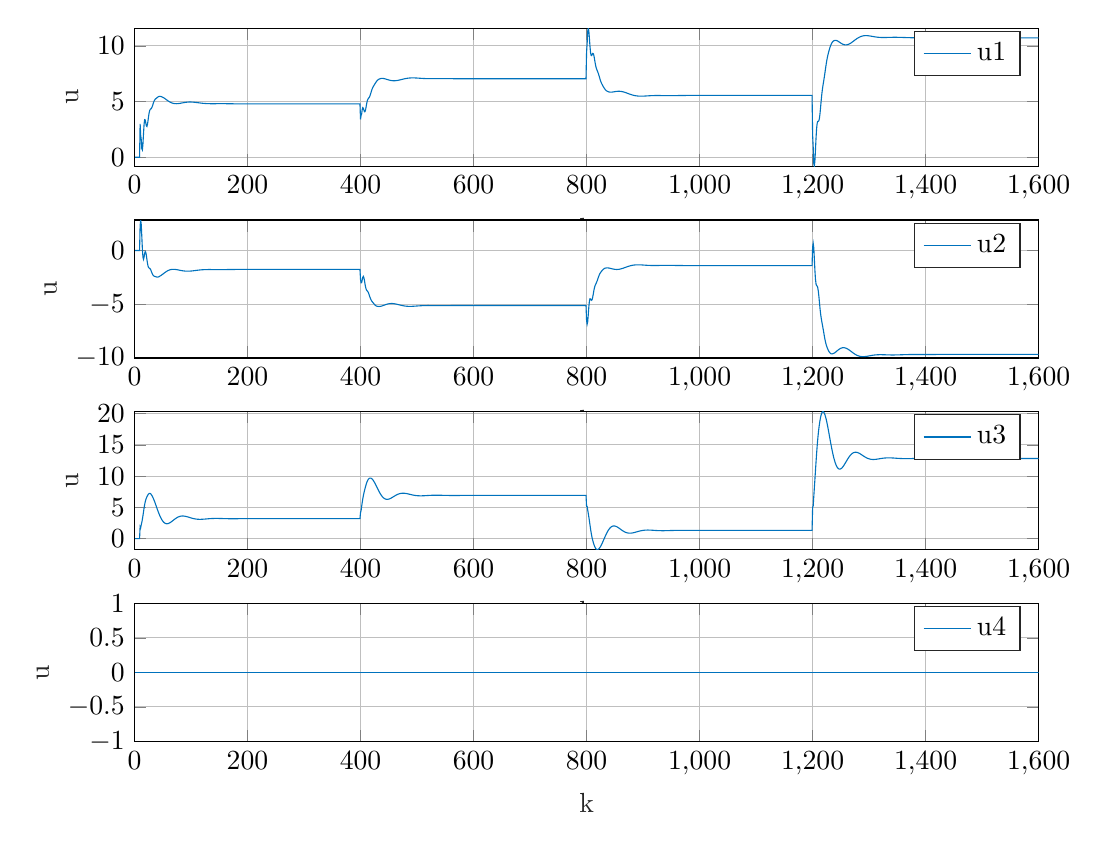
\begin{tikzpicture}

\begin{axis}[%
width=4.521in,
height=0.69in,
at={(0.758in,3.357in)},
scale only axis,
xmin=0,
xmax=1600,
xlabel style={font=\color{white!15!black}},
xlabel={k},
ymin=-0.80079,
ymax=11.581,
ylabel style={font=\color{white!15!black}},
ylabel={u},
axis background/.style={fill=white},
xmajorgrids,
ymajorgrids,
legend style={legend cell align=left, align=left, draw=white!15!black}
]
\addplot [color=mycolor1]
  table[row sep=crcr]{%
1	0\\
2	0\\
3	0\\
4	0\\
5	0\\
6	0\\
7	0\\
8	0\\
9	0\\
10	2.9925\\
11	1.9651\\
12	1.5955\\
13	0.75662\\
14	0.65506\\
15	1.2101\\
16	2.1365\\
17	2.958\\
18	3.3746\\
19	3.3551\\
20	3.0879\\
21	2.8302\\
22	2.768\\
23	2.9489\\
24	3.2981\\
25	3.6867\\
26	4.0042\\
27	4.2022\\
28	4.297\\
29	4.3433\\
30	4.3982\\
31	4.4947\\
32	4.6344\\
33	4.7954\\
34	4.9491\\
35	5.0742\\
36	5.164\\
37	5.2248\\
38	5.2692\\
39	5.3087\\
40	5.3494\\
41	5.3907\\
42	5.4279\\
43	5.4557\\
44	5.471\\
45	5.4734\\
46	5.4656\\
47	5.4507\\
48	5.4317\\
49	5.4101\\
50	5.3862\\
51	5.3596\\
52	5.3298\\
53	5.2967\\
54	5.2609\\
55	5.2236\\
56	5.1858\\
57	5.1485\\
58	5.1121\\
59	5.0771\\
60	5.0435\\
61	5.0115\\
62	4.9812\\
63	4.9529\\
64	4.9269\\
65	4.9034\\
66	4.8826\\
67	4.8645\\
68	4.8492\\
69	4.8365\\
70	4.8264\\
71	4.8188\\
72	4.8135\\
73	4.8104\\
74	4.8095\\
75	4.8105\\
76	4.8133\\
77	4.8176\\
78	4.8233\\
79	4.8302\\
80	4.838\\
81	4.8465\\
82	4.8556\\
83	4.865\\
84	4.8747\\
85	4.8843\\
86	4.8939\\
87	4.9031\\
88	4.9119\\
89	4.9202\\
90	4.9279\\
91	4.9349\\
92	4.941\\
93	4.9464\\
94	4.9508\\
95	4.9544\\
96	4.957\\
97	4.9587\\
98	4.9595\\
99	4.9594\\
100	4.9585\\
101	4.9568\\
102	4.9542\\
103	4.951\\
104	4.9472\\
105	4.9427\\
106	4.9377\\
107	4.9323\\
108	4.9265\\
109	4.9204\\
110	4.9141\\
111	4.9076\\
112	4.901\\
113	4.8943\\
114	4.8877\\
115	4.8812\\
116	4.8747\\
117	4.8685\\
118	4.8624\\
119	4.8566\\
120	4.8511\\
121	4.8459\\
122	4.841\\
123	4.8365\\
124	4.8323\\
125	4.8285\\
126	4.825\\
127	4.8219\\
128	4.8192\\
129	4.8167\\
130	4.8147\\
131	4.8129\\
132	4.8115\\
133	4.8103\\
134	4.8094\\
135	4.8087\\
136	4.8082\\
137	4.8079\\
138	4.8078\\
139	4.8079\\
140	4.808\\
141	4.8083\\
142	4.8086\\
143	4.809\\
144	4.8094\\
145	4.8098\\
146	4.8102\\
147	4.8107\\
148	4.811\\
149	4.8114\\
150	4.8117\\
151	4.8119\\
152	4.8121\\
153	4.8122\\
154	4.8122\\
155	4.8121\\
156	4.812\\
157	4.8118\\
158	4.8115\\
159	4.8112\\
160	4.8107\\
161	4.8102\\
162	4.8097\\
163	4.8091\\
164	4.8084\\
165	4.8078\\
166	4.807\\
167	4.8063\\
168	4.8055\\
169	4.8047\\
170	4.8039\\
171	4.8032\\
172	4.8024\\
173	4.8016\\
174	4.8009\\
175	4.8001\\
176	4.7994\\
177	4.7987\\
178	4.7981\\
179	4.7975\\
180	4.7969\\
181	4.7964\\
182	4.7959\\
183	4.7955\\
184	4.7951\\
185	4.7948\\
186	4.7945\\
187	4.7942\\
188	4.794\\
189	4.7938\\
190	4.7936\\
191	4.7935\\
192	4.7934\\
193	4.7934\\
194	4.7933\\
195	4.7933\\
196	4.7934\\
197	4.7934\\
198	4.7934\\
199	4.7935\\
200	4.7936\\
201	4.7937\\
202	4.7938\\
203	4.7939\\
204	4.7939\\
205	4.794\\
206	4.7941\\
207	4.7942\\
208	4.7943\\
209	4.7944\\
210	4.7945\\
211	4.7945\\
212	4.7946\\
213	4.7946\\
214	4.7947\\
215	4.7947\\
216	4.7947\\
217	4.7947\\
218	4.7947\\
219	4.7947\\
220	4.7947\\
221	4.7947\\
222	4.7947\\
223	4.7947\\
224	4.7946\\
225	4.7946\\
226	4.7946\\
227	4.7945\\
228	4.7945\\
229	4.7944\\
230	4.7944\\
231	4.7943\\
232	4.7943\\
233	4.7942\\
234	4.7942\\
235	4.7941\\
236	4.7941\\
237	4.7941\\
238	4.794\\
239	4.794\\
240	4.794\\
241	4.794\\
242	4.7939\\
243	4.7939\\
244	4.7939\\
245	4.7939\\
246	4.7939\\
247	4.7939\\
248	4.7939\\
249	4.7939\\
250	4.7939\\
251	4.7939\\
252	4.794\\
253	4.794\\
254	4.794\\
255	4.794\\
256	4.794\\
257	4.7941\\
258	4.7941\\
259	4.7941\\
260	4.7941\\
261	4.7942\\
262	4.7942\\
263	4.7942\\
264	4.7942\\
265	4.7943\\
266	4.7943\\
267	4.7943\\
268	4.7943\\
269	4.7944\\
270	4.7944\\
271	4.7944\\
272	4.7944\\
273	4.7944\\
274	4.7944\\
275	4.7944\\
276	4.7945\\
277	4.7945\\
278	4.7945\\
279	4.7945\\
280	4.7945\\
281	4.7945\\
282	4.7945\\
283	4.7945\\
284	4.7945\\
285	4.7945\\
286	4.7945\\
287	4.7945\\
288	4.7945\\
289	4.7945\\
290	4.7945\\
291	4.7945\\
292	4.7945\\
293	4.7945\\
294	4.7945\\
295	4.7945\\
296	4.7945\\
297	4.7945\\
298	4.7945\\
299	4.7945\\
300	4.7945\\
301	4.7945\\
302	4.7945\\
303	4.7945\\
304	4.7945\\
305	4.7945\\
306	4.7945\\
307	4.7945\\
308	4.7945\\
309	4.7945\\
310	4.7945\\
311	4.7945\\
312	4.7945\\
313	4.7945\\
314	4.7945\\
315	4.7946\\
316	4.7946\\
317	4.7946\\
318	4.7946\\
319	4.7946\\
320	4.7946\\
321	4.7946\\
322	4.7946\\
323	4.7946\\
324	4.7946\\
325	4.7946\\
326	4.7946\\
327	4.7946\\
328	4.7946\\
329	4.7946\\
330	4.7946\\
331	4.7946\\
332	4.7946\\
333	4.7946\\
334	4.7946\\
335	4.7946\\
336	4.7946\\
337	4.7946\\
338	4.7946\\
339	4.7946\\
340	4.7946\\
341	4.7946\\
342	4.7946\\
343	4.7946\\
344	4.7946\\
345	4.7946\\
346	4.7946\\
347	4.7946\\
348	4.7946\\
349	4.7946\\
350	4.7946\\
351	4.7946\\
352	4.7946\\
353	4.7946\\
354	4.7946\\
355	4.7946\\
356	4.7946\\
357	4.7946\\
358	4.7946\\
359	4.7946\\
360	4.7946\\
361	4.7946\\
362	4.7946\\
363	4.7946\\
364	4.7946\\
365	4.7946\\
366	4.7946\\
367	4.7946\\
368	4.7946\\
369	4.7946\\
370	4.7946\\
371	4.7946\\
372	4.7946\\
373	4.7946\\
374	4.7946\\
375	4.7946\\
376	4.7946\\
377	4.7946\\
378	4.7946\\
379	4.7946\\
380	4.7946\\
381	4.7946\\
382	4.7946\\
383	4.7946\\
384	4.7946\\
385	4.7946\\
386	4.7946\\
387	4.7946\\
388	4.7946\\
389	4.7946\\
390	4.7946\\
391	4.7946\\
392	4.7946\\
393	4.7946\\
394	4.7946\\
395	4.7946\\
396	4.7946\\
397	4.7946\\
398	4.7946\\
399	4.7946\\
400	3.3981\\
401	3.7633\\
402	3.8863\\
403	4.2873\\
404	4.4569\\
405	4.4063\\
406	4.2239\\
407	4.0828\\
408	4.0959\\
409	4.2779\\
410	4.5608\\
411	4.849\\
412	5.0721\\
413	5.2098\\
414	5.2872\\
415	5.3496\\
416	5.4359\\
417	5.5622\\
418	5.7211\\
419	5.8911\\
420	6.0501\\
421	6.185\\
422	6.2943\\
423	6.3853\\
424	6.4681\\
425	6.55\\
426	6.6332\\
427	6.7152\\
428	6.7913\\
429	6.8575\\
430	6.9119\\
431	6.9549\\
432	6.9888\\
433	7.0161\\
434	7.0384\\
435	7.0566\\
436	7.0704\\
437	7.0794\\
438	7.0833\\
439	7.0821\\
440	7.0768\\
441	7.0681\\
442	7.0571\\
443	7.0444\\
444	7.0305\\
445	7.0158\\
446	7.0004\\
447	6.9846\\
448	6.9687\\
449	6.9531\\
450	6.9382\\
451	6.9243\\
452	6.9117\\
453	6.9005\\
454	6.8909\\
455	6.8829\\
456	6.8765\\
457	6.8719\\
458	6.869\\
459	6.8678\\
460	6.8684\\
461	6.8707\\
462	6.8745\\
463	6.8798\\
464	6.8865\\
465	6.8944\\
466	6.9034\\
467	6.9133\\
468	6.9241\\
469	6.9355\\
470	6.9474\\
471	6.9597\\
472	6.9723\\
473	6.9849\\
474	6.9975\\
475	7.0099\\
476	7.022\\
477	7.0337\\
478	7.0449\\
479	7.0556\\
480	7.0656\\
481	7.0749\\
482	7.0835\\
483	7.0913\\
484	7.0982\\
485	7.1044\\
486	7.1097\\
487	7.1141\\
488	7.1178\\
489	7.1206\\
490	7.1227\\
491	7.124\\
492	7.1246\\
493	7.1246\\
494	7.124\\
495	7.1229\\
496	7.1212\\
497	7.1191\\
498	7.1166\\
499	7.1139\\
500	7.1108\\
501	7.1075\\
502	7.1041\\
503	7.1005\\
504	7.0969\\
505	7.0933\\
506	7.0897\\
507	7.0862\\
508	7.0828\\
509	7.0795\\
510	7.0763\\
511	7.0734\\
512	7.0706\\
513	7.0681\\
514	7.0657\\
515	7.0636\\
516	7.0617\\
517	7.0601\\
518	7.0587\\
519	7.0575\\
520	7.0565\\
521	7.0557\\
522	7.0551\\
523	7.0547\\
524	7.0545\\
525	7.0544\\
526	7.0544\\
527	7.0546\\
528	7.0549\\
529	7.0552\\
530	7.0557\\
531	7.0561\\
532	7.0566\\
533	7.0572\\
534	7.0577\\
535	7.0582\\
536	7.0587\\
537	7.0592\\
538	7.0597\\
539	7.0601\\
540	7.0604\\
541	7.0607\\
542	7.0609\\
543	7.0611\\
544	7.0612\\
545	7.0612\\
546	7.0612\\
547	7.061\\
548	7.0609\\
549	7.0606\\
550	7.0603\\
551	7.0599\\
552	7.0595\\
553	7.0591\\
554	7.0586\\
555	7.058\\
556	7.0575\\
557	7.0569\\
558	7.0562\\
559	7.0556\\
560	7.055\\
561	7.0543\\
562	7.0537\\
563	7.0531\\
564	7.0525\\
565	7.0518\\
566	7.0513\\
567	7.0507\\
568	7.0501\\
569	7.0496\\
570	7.0491\\
571	7.0487\\
572	7.0483\\
573	7.0479\\
574	7.0475\\
575	7.0472\\
576	7.0469\\
577	7.0466\\
578	7.0464\\
579	7.0462\\
580	7.046\\
581	7.0458\\
582	7.0457\\
583	7.0456\\
584	7.0455\\
585	7.0455\\
586	7.0454\\
587	7.0454\\
588	7.0454\\
589	7.0453\\
590	7.0453\\
591	7.0454\\
592	7.0454\\
593	7.0454\\
594	7.0454\\
595	7.0454\\
596	7.0454\\
597	7.0455\\
598	7.0455\\
599	7.0455\\
600	7.0455\\
601	7.0455\\
602	7.0455\\
603	7.0455\\
604	7.0455\\
605	7.0454\\
606	7.0454\\
607	7.0454\\
608	7.0453\\
609	7.0453\\
610	7.0452\\
611	7.0452\\
612	7.0451\\
613	7.0451\\
614	7.045\\
615	7.045\\
616	7.0449\\
617	7.0448\\
618	7.0448\\
619	7.0447\\
620	7.0446\\
621	7.0446\\
622	7.0445\\
623	7.0444\\
624	7.0444\\
625	7.0443\\
626	7.0443\\
627	7.0442\\
628	7.0442\\
629	7.0441\\
630	7.0441\\
631	7.044\\
632	7.044\\
633	7.044\\
634	7.044\\
635	7.0439\\
636	7.0439\\
637	7.0439\\
638	7.0439\\
639	7.0439\\
640	7.0439\\
641	7.0439\\
642	7.0439\\
643	7.0439\\
644	7.0439\\
645	7.0439\\
646	7.0439\\
647	7.0439\\
648	7.0439\\
649	7.0439\\
650	7.0439\\
651	7.0439\\
652	7.0439\\
653	7.0439\\
654	7.0439\\
655	7.0439\\
656	7.044\\
657	7.044\\
658	7.044\\
659	7.044\\
660	7.044\\
661	7.044\\
662	7.044\\
663	7.044\\
664	7.044\\
665	7.044\\
666	7.044\\
667	7.044\\
668	7.044\\
669	7.044\\
670	7.044\\
671	7.044\\
672	7.044\\
673	7.044\\
674	7.044\\
675	7.044\\
676	7.044\\
677	7.044\\
678	7.044\\
679	7.044\\
680	7.044\\
681	7.044\\
682	7.044\\
683	7.044\\
684	7.044\\
685	7.044\\
686	7.044\\
687	7.044\\
688	7.044\\
689	7.044\\
690	7.044\\
691	7.044\\
692	7.044\\
693	7.044\\
694	7.044\\
695	7.044\\
696	7.044\\
697	7.044\\
698	7.044\\
699	7.044\\
700	7.044\\
701	7.044\\
702	7.044\\
703	7.044\\
704	7.044\\
705	7.044\\
706	7.044\\
707	7.044\\
708	7.044\\
709	7.044\\
710	7.044\\
711	7.044\\
712	7.044\\
713	7.044\\
714	7.044\\
715	7.044\\
716	7.044\\
717	7.044\\
718	7.044\\
719	7.044\\
720	7.044\\
721	7.044\\
722	7.044\\
723	7.044\\
724	7.044\\
725	7.044\\
726	7.044\\
727	7.044\\
728	7.044\\
729	7.044\\
730	7.044\\
731	7.044\\
732	7.044\\
733	7.044\\
734	7.044\\
735	7.0441\\
736	7.0441\\
737	7.0441\\
738	7.0441\\
739	7.0441\\
740	7.0441\\
741	7.0441\\
742	7.0441\\
743	7.0441\\
744	7.0441\\
745	7.0441\\
746	7.0441\\
747	7.0441\\
748	7.0441\\
749	7.0441\\
750	7.0441\\
751	7.0441\\
752	7.0441\\
753	7.0441\\
754	7.0441\\
755	7.0441\\
756	7.0441\\
757	7.0441\\
758	7.0441\\
759	7.0441\\
760	7.0441\\
761	7.0441\\
762	7.0441\\
763	7.0441\\
764	7.0441\\
765	7.0441\\
766	7.0441\\
767	7.0441\\
768	7.0441\\
769	7.0441\\
770	7.0441\\
771	7.0441\\
772	7.0441\\
773	7.0441\\
774	7.0441\\
775	7.0441\\
776	7.0441\\
777	7.0441\\
778	7.0441\\
779	7.0441\\
780	7.0441\\
781	7.0441\\
782	7.0441\\
783	7.0441\\
784	7.0441\\
785	7.0441\\
786	7.0441\\
787	7.0441\\
788	7.0441\\
789	7.0441\\
790	7.0441\\
791	7.0441\\
792	7.0441\\
793	7.0441\\
794	7.0441\\
795	7.0441\\
796	7.0441\\
797	7.0441\\
798	7.0441\\
799	7.0441\\
800	9.4381\\
801	10.219\\
802	11.315\\
803	11.581\\
804	11.328\\
805	10.688\\
806	9.971\\
807	9.4157\\
808	9.1428\\
809	9.1245\\
810	9.2341\\
811	9.3235\\
812	9.291\\
813	9.1127\\
814	8.8314\\
815	8.5201\\
816	8.243\\
817	8.0309\\
818	7.8781\\
819	7.7564\\
820	7.6342\\
821	7.4918\\
822	7.3268\\
823	7.1504\\
824	6.9787\\
825	6.8245\\
826	6.693\\
827	6.5818\\
828	6.4846\\
829	6.3948\\
830	6.3088\\
831	6.2264\\
832	6.1499\\
833	6.0823\\
834	6.0254\\
835	5.9794\\
836	5.9431\\
837	5.9145\\
838	5.8918\\
839	5.8737\\
840	5.8599\\
841	5.8502\\
842	5.8448\\
843	5.8434\\
844	5.8456\\
845	5.8504\\
846	5.8571\\
847	5.865\\
848	5.8734\\
849	5.882\\
850	5.8905\\
851	5.8987\\
852	5.9062\\
853	5.9129\\
854	5.9184\\
855	5.9225\\
856	5.925\\
857	5.9258\\
858	5.9247\\
859	5.9218\\
860	5.9171\\
861	5.9107\\
862	5.9026\\
863	5.8927\\
864	5.8814\\
865	5.8686\\
866	5.8544\\
867	5.8391\\
868	5.8228\\
869	5.8057\\
870	5.7879\\
871	5.7695\\
872	5.7509\\
873	5.7321\\
874	5.7132\\
875	5.6945\\
876	5.6761\\
877	5.6581\\
878	5.6406\\
879	5.6238\\
880	5.6078\\
881	5.5925\\
882	5.5782\\
883	5.5649\\
884	5.5526\\
885	5.5413\\
886	5.5312\\
887	5.5221\\
888	5.514\\
889	5.5071\\
890	5.5012\\
891	5.4963\\
892	5.4923\\
893	5.4893\\
894	5.4872\\
895	5.4858\\
896	5.4853\\
897	5.4854\\
898	5.4861\\
899	5.4873\\
900	5.4891\\
901	5.4912\\
902	5.4937\\
903	5.4965\\
904	5.4995\\
905	5.5026\\
906	5.5059\\
907	5.5092\\
908	5.5124\\
909	5.5157\\
910	5.5188\\
911	5.5218\\
912	5.5247\\
913	5.5274\\
914	5.5299\\
915	5.5322\\
916	5.5342\\
917	5.536\\
918	5.5376\\
919	5.539\\
920	5.5401\\
921	5.541\\
922	5.5416\\
923	5.5421\\
924	5.5423\\
925	5.5424\\
926	5.5424\\
927	5.5421\\
928	5.5418\\
929	5.5413\\
930	5.5408\\
931	5.5402\\
932	5.5395\\
933	5.5388\\
934	5.5381\\
935	5.5373\\
936	5.5366\\
937	5.5359\\
938	5.5353\\
939	5.5347\\
940	5.5341\\
941	5.5336\\
942	5.5332\\
943	5.5329\\
944	5.5327\\
945	5.5325\\
946	5.5324\\
947	5.5325\\
948	5.5326\\
949	5.5327\\
950	5.533\\
951	5.5334\\
952	5.5338\\
953	5.5343\\
954	5.5348\\
955	5.5354\\
956	5.5361\\
957	5.5367\\
958	5.5375\\
959	5.5382\\
960	5.539\\
961	5.5398\\
962	5.5406\\
963	5.5414\\
964	5.5422\\
965	5.543\\
966	5.5438\\
967	5.5445\\
968	5.5453\\
969	5.546\\
970	5.5466\\
971	5.5473\\
972	5.5479\\
973	5.5485\\
974	5.549\\
975	5.5495\\
976	5.55\\
977	5.5504\\
978	5.5508\\
979	5.5512\\
980	5.5515\\
981	5.5518\\
982	5.552\\
983	5.5522\\
984	5.5524\\
985	5.5526\\
986	5.5527\\
987	5.5529\\
988	5.553\\
989	5.5531\\
990	5.5531\\
991	5.5532\\
992	5.5532\\
993	5.5533\\
994	5.5533\\
995	5.5533\\
996	5.5534\\
997	5.5534\\
998	5.5534\\
999	5.5534\\
1000	5.5535\\
1001	5.5535\\
1002	5.5535\\
1003	5.5536\\
1004	5.5536\\
1005	5.5537\\
1006	5.5537\\
1007	5.5538\\
1008	5.5539\\
1009	5.5539\\
1010	5.554\\
1011	5.5541\\
1012	5.5542\\
1013	5.5543\\
1014	5.5544\\
1015	5.5545\\
1016	5.5546\\
1017	5.5547\\
1018	5.5548\\
1019	5.5549\\
1020	5.555\\
1021	5.5551\\
1022	5.5552\\
1023	5.5553\\
1024	5.5554\\
1025	5.5555\\
1026	5.5556\\
1027	5.5557\\
1028	5.5557\\
1029	5.5558\\
1030	5.5559\\
1031	5.556\\
1032	5.556\\
1033	5.5561\\
1034	5.5561\\
1035	5.5562\\
1036	5.5562\\
1037	5.5563\\
1038	5.5563\\
1039	5.5563\\
1040	5.5564\\
1041	5.5564\\
1042	5.5564\\
1043	5.5564\\
1044	5.5564\\
1045	5.5564\\
1046	5.5564\\
1047	5.5565\\
1048	5.5565\\
1049	5.5565\\
1050	5.5565\\
1051	5.5565\\
1052	5.5564\\
1053	5.5564\\
1054	5.5564\\
1055	5.5564\\
1056	5.5564\\
1057	5.5564\\
1058	5.5564\\
1059	5.5564\\
1060	5.5564\\
1061	5.5564\\
1062	5.5564\\
1063	5.5564\\
1064	5.5564\\
1065	5.5564\\
1066	5.5564\\
1067	5.5564\\
1068	5.5564\\
1069	5.5564\\
1070	5.5564\\
1071	5.5564\\
1072	5.5564\\
1073	5.5564\\
1074	5.5564\\
1075	5.5564\\
1076	5.5564\\
1077	5.5564\\
1078	5.5564\\
1079	5.5564\\
1080	5.5564\\
1081	5.5564\\
1082	5.5565\\
1083	5.5565\\
1084	5.5565\\
1085	5.5565\\
1086	5.5565\\
1087	5.5565\\
1088	5.5565\\
1089	5.5565\\
1090	5.5565\\
1091	5.5565\\
1092	5.5565\\
1093	5.5565\\
1094	5.5565\\
1095	5.5565\\
1096	5.5565\\
1097	5.5565\\
1098	5.5565\\
1099	5.5565\\
1100	5.5565\\
1101	5.5565\\
1102	5.5565\\
1103	5.5565\\
1104	5.5565\\
1105	5.5565\\
1106	5.5565\\
1107	5.5565\\
1108	5.5565\\
1109	5.5565\\
1110	5.5565\\
1111	5.5565\\
1112	5.5565\\
1113	5.5564\\
1114	5.5564\\
1115	5.5564\\
1116	5.5564\\
1117	5.5564\\
1118	5.5564\\
1119	5.5564\\
1120	5.5564\\
1121	5.5564\\
1122	5.5564\\
1123	5.5564\\
1124	5.5564\\
1125	5.5564\\
1126	5.5564\\
1127	5.5564\\
1128	5.5564\\
1129	5.5564\\
1130	5.5564\\
1131	5.5564\\
1132	5.5564\\
1133	5.5564\\
1134	5.5564\\
1135	5.5564\\
1136	5.5564\\
1137	5.5564\\
1138	5.5564\\
1139	5.5564\\
1140	5.5564\\
1141	5.5564\\
1142	5.5564\\
1143	5.5564\\
1144	5.5564\\
1145	5.5564\\
1146	5.5564\\
1147	5.5564\\
1148	5.5564\\
1149	5.5564\\
1150	5.5564\\
1151	5.5564\\
1152	5.5564\\
1153	5.5564\\
1154	5.5564\\
1155	5.5564\\
1156	5.5564\\
1157	5.5564\\
1158	5.5564\\
1159	5.5564\\
1160	5.5564\\
1161	5.5564\\
1162	5.5564\\
1163	5.5564\\
1164	5.5564\\
1165	5.5564\\
1166	5.5564\\
1167	5.5564\\
1168	5.5564\\
1169	5.5564\\
1170	5.5564\\
1171	5.5564\\
1172	5.5564\\
1173	5.5564\\
1174	5.5564\\
1175	5.5564\\
1176	5.5564\\
1177	5.5564\\
1178	5.5564\\
1179	5.5564\\
1180	5.5564\\
1181	5.5564\\
1182	5.5564\\
1183	5.5564\\
1184	5.5564\\
1185	5.5564\\
1186	5.5564\\
1187	5.5564\\
1188	5.5564\\
1189	5.5564\\
1190	5.5564\\
1191	5.5564\\
1192	5.5564\\
1193	5.5564\\
1194	5.5564\\
1195	5.5564\\
1196	5.5564\\
1197	5.5564\\
1198	5.5564\\
1199	5.5564\\
1200	1.9654\\
1201	0.93482\\
1202	-0.54652\\
1203	-0.80079\\
1204	-0.34519\\
1205	0.62807\\
1206	1.6967\\
1207	2.5523\\
1208	3.0444\\
1209	3.2145\\
1210	3.2281\\
1211	3.2762\\
1212	3.4878\\
1213	3.8915\\
1214	4.4301\\
1215	5.0074\\
1216	5.539\\
1217	5.9837\\
1218	6.3473\\
1219	6.665\\
1220	6.9766\\
1221	7.3067\\
1222	7.6578\\
1223	8.0151\\
1224	8.3573\\
1225	8.6673\\
1226	8.9382\\
1227	9.1727\\
1228	9.3792\\
1229	9.5661\\
1230	9.7383\\
1231	9.8965\\
1232	10.038\\
1233	10.16\\
1234	10.259\\
1235	10.337\\
1236	10.395\\
1237	10.438\\
1238	10.466\\
1239	10.484\\
1240	10.492\\
1241	10.491\\
1242	10.481\\
1243	10.464\\
1244	10.44\\
1245	10.411\\
1246	10.379\\
1247	10.345\\
1248	10.311\\
1249	10.277\\
1250	10.244\\
1251	10.213\\
1252	10.184\\
1253	10.158\\
1254	10.136\\
1255	10.117\\
1256	10.103\\
1257	10.093\\
1258	10.088\\
1259	10.088\\
1260	10.092\\
1261	10.101\\
1262	10.113\\
1263	10.13\\
1264	10.151\\
1265	10.175\\
1266	10.202\\
1267	10.232\\
1268	10.265\\
1269	10.299\\
1270	10.335\\
1271	10.373\\
1272	10.411\\
1273	10.449\\
1274	10.488\\
1275	10.526\\
1276	10.563\\
1277	10.6\\
1278	10.635\\
1279	10.669\\
1280	10.701\\
1281	10.731\\
1282	10.759\\
1283	10.785\\
1284	10.809\\
1285	10.83\\
1286	10.849\\
1287	10.865\\
1288	10.879\\
1289	10.891\\
1290	10.901\\
1291	10.908\\
1292	10.913\\
1293	10.916\\
1294	10.918\\
1295	10.917\\
1296	10.915\\
1297	10.912\\
1298	10.908\\
1299	10.902\\
1300	10.895\\
1301	10.888\\
1302	10.88\\
1303	10.871\\
1304	10.863\\
1305	10.854\\
1306	10.845\\
1307	10.836\\
1308	10.827\\
1309	10.818\\
1310	10.81\\
1311	10.802\\
1312	10.794\\
1313	10.787\\
1314	10.781\\
1315	10.775\\
1316	10.77\\
1317	10.765\\
1318	10.761\\
1319	10.758\\
1320	10.755\\
1321	10.752\\
1322	10.751\\
1323	10.749\\
1324	10.749\\
1325	10.748\\
1326	10.748\\
1327	10.749\\
1328	10.749\\
1329	10.75\\
1330	10.751\\
1331	10.753\\
1332	10.754\\
1333	10.755\\
1334	10.757\\
1335	10.759\\
1336	10.76\\
1337	10.761\\
1338	10.763\\
1339	10.764\\
1340	10.765\\
1341	10.766\\
1342	10.767\\
1343	10.768\\
1344	10.768\\
1345	10.768\\
1346	10.768\\
1347	10.768\\
1348	10.768\\
1349	10.767\\
1350	10.766\\
1351	10.765\\
1352	10.764\\
1353	10.763\\
1354	10.762\\
1355	10.76\\
1356	10.759\\
1357	10.757\\
1358	10.756\\
1359	10.754\\
1360	10.752\\
1361	10.75\\
1362	10.748\\
1363	10.747\\
1364	10.745\\
1365	10.743\\
1366	10.741\\
1367	10.74\\
1368	10.738\\
1369	10.736\\
1370	10.735\\
1371	10.734\\
1372	10.732\\
1373	10.731\\
1374	10.73\\
1375	10.729\\
1376	10.728\\
1377	10.727\\
1378	10.726\\
1379	10.726\\
1380	10.725\\
1381	10.724\\
1382	10.724\\
1383	10.724\\
1384	10.723\\
1385	10.723\\
1386	10.723\\
1387	10.722\\
1388	10.722\\
1389	10.722\\
1390	10.722\\
1391	10.722\\
1392	10.722\\
1393	10.722\\
1394	10.722\\
1395	10.722\\
1396	10.722\\
1397	10.722\\
1398	10.722\\
1399	10.722\\
1400	10.722\\
1401	10.722\\
1402	10.722\\
1403	10.722\\
1404	10.722\\
1405	10.722\\
1406	10.722\\
1407	10.722\\
1408	10.721\\
1409	10.721\\
1410	10.721\\
1411	10.721\\
1412	10.721\\
1413	10.721\\
1414	10.72\\
1415	10.72\\
1416	10.72\\
1417	10.72\\
1418	10.72\\
1419	10.719\\
1420	10.719\\
1421	10.719\\
1422	10.719\\
1423	10.719\\
1424	10.718\\
1425	10.718\\
1426	10.718\\
1427	10.718\\
1428	10.718\\
1429	10.718\\
1430	10.717\\
1431	10.717\\
1432	10.717\\
1433	10.717\\
1434	10.717\\
1435	10.717\\
1436	10.717\\
1437	10.717\\
1438	10.717\\
1439	10.717\\
1440	10.717\\
1441	10.717\\
1442	10.717\\
1443	10.717\\
1444	10.717\\
1445	10.717\\
1446	10.717\\
1447	10.717\\
1448	10.717\\
1449	10.717\\
1450	10.717\\
1451	10.717\\
1452	10.717\\
1453	10.717\\
1454	10.717\\
1455	10.717\\
1456	10.717\\
1457	10.717\\
1458	10.717\\
1459	10.717\\
1460	10.717\\
1461	10.717\\
1462	10.717\\
1463	10.717\\
1464	10.717\\
1465	10.717\\
1466	10.717\\
1467	10.717\\
1468	10.717\\
1469	10.717\\
1470	10.717\\
1471	10.717\\
1472	10.717\\
1473	10.717\\
1474	10.717\\
1475	10.717\\
1476	10.717\\
1477	10.717\\
1478	10.717\\
1479	10.717\\
1480	10.717\\
1481	10.717\\
1482	10.717\\
1483	10.717\\
1484	10.717\\
1485	10.717\\
1486	10.717\\
1487	10.717\\
1488	10.717\\
1489	10.717\\
1490	10.717\\
1491	10.717\\
1492	10.717\\
1493	10.717\\
1494	10.717\\
1495	10.717\\
1496	10.717\\
1497	10.717\\
1498	10.717\\
1499	10.717\\
1500	10.717\\
1501	10.717\\
1502	10.717\\
1503	10.717\\
1504	10.717\\
1505	10.717\\
1506	10.717\\
1507	10.717\\
1508	10.717\\
1509	10.717\\
1510	10.717\\
1511	10.717\\
1512	10.717\\
1513	10.717\\
1514	10.717\\
1515	10.717\\
1516	10.717\\
1517	10.717\\
1518	10.717\\
1519	10.717\\
1520	10.717\\
1521	10.717\\
1522	10.717\\
1523	10.717\\
1524	10.717\\
1525	10.717\\
1526	10.717\\
1527	10.717\\
1528	10.717\\
1529	10.717\\
1530	10.717\\
1531	10.717\\
1532	10.717\\
1533	10.717\\
1534	10.717\\
1535	10.717\\
1536	10.717\\
1537	10.717\\
1538	10.717\\
1539	10.717\\
1540	10.717\\
1541	10.717\\
1542	10.717\\
1543	10.717\\
1544	10.717\\
1545	10.717\\
1546	10.717\\
1547	10.717\\
1548	10.717\\
1549	10.717\\
1550	10.717\\
1551	10.717\\
1552	10.717\\
1553	10.717\\
1554	10.717\\
1555	10.717\\
1556	10.717\\
1557	10.717\\
1558	10.717\\
1559	10.717\\
1560	10.717\\
1561	10.717\\
1562	10.717\\
1563	10.717\\
1564	10.717\\
1565	10.717\\
1566	10.717\\
1567	10.717\\
1568	10.717\\
1569	10.717\\
1570	10.717\\
1571	10.717\\
1572	10.717\\
1573	10.717\\
1574	10.717\\
1575	10.717\\
1576	10.717\\
1577	10.717\\
1578	10.717\\
1579	10.717\\
1580	10.717\\
1581	10.717\\
1582	10.717\\
1583	10.717\\
1584	10.717\\
1585	10.717\\
1586	10.717\\
1587	10.717\\
1588	10.717\\
1589	10.717\\
1590	10.717\\
1591	10.717\\
1592	10.717\\
1593	10.717\\
1594	10.717\\
1595	10.717\\
1596	10.717\\
1597	10.717\\
1598	10.717\\
1599	10.717\\
1600	10.717\\
};
\addlegendentry{u1}

\end{axis}

\begin{axis}[%
width=4.521in,
height=0.69in,
at={(0.758in,2.398in)},
scale only axis,
xmin=0,
xmax=1600,
xlabel style={font=\color{white!15!black}},
xlabel={k},
ymin=-10,
ymax=2.8325,
ylabel style={font=\color{white!15!black}},
ylabel={u},
axis background/.style={fill=white},
xmajorgrids,
ymajorgrids,
legend style={legend cell align=left, align=left, draw=white!15!black}
]
\addplot [color=mycolor1]
  table[row sep=crcr]{%
1	0\\
2	0\\
3	0\\
4	0\\
5	0\\
6	0\\
7	0\\
8	0\\
9	0\\
10	2.32\\
11	2.8325\\
12	2.3958\\
13	1.2824\\
14	0.12599\\
15	-0.62141\\
16	-0.821\\
17	-0.61817\\
18	-0.29347\\
19	-0.098827\\
20	-0.15478\\
21	-0.43601\\
22	-0.82518\\
23	-1.1911\\
24	-1.4498\\
25	-1.5862\\
26	-1.6401\\
27	-1.6716\\
28	-1.7285\\
29	-1.8289\\
30	-1.9621\\
31	-2.1016\\
32	-2.2214\\
33	-2.3073\\
34	-2.3595\\
35	-2.3882\\
36	-2.4063\\
37	-2.4233\\
38	-2.442\\
39	-2.46\\
40	-2.4721\\
41	-2.4741\\
42	-2.4643\\
43	-2.444\\
44	-2.4162\\
45	-2.3844\\
46	-2.3508\\
47	-2.3163\\
48	-2.2808\\
49	-2.2439\\
50	-2.2052\\
51	-2.1649\\
52	-2.1239\\
53	-2.0832\\
54	-2.0437\\
55	-2.0061\\
56	-1.9709\\
57	-1.938\\
58	-1.9075\\
59	-1.8794\\
60	-1.8538\\
61	-1.831\\
62	-1.811\\
63	-1.794\\
64	-1.78\\
65	-1.769\\
66	-1.7607\\
67	-1.7551\\
68	-1.7519\\
69	-1.751\\
70	-1.7522\\
71	-1.7553\\
72	-1.7602\\
73	-1.7666\\
74	-1.7743\\
75	-1.7831\\
76	-1.7927\\
77	-1.803\\
78	-1.8136\\
79	-1.8245\\
80	-1.8354\\
81	-1.8463\\
82	-1.8568\\
83	-1.8669\\
84	-1.8764\\
85	-1.8853\\
86	-1.8934\\
87	-1.9007\\
88	-1.907\\
89	-1.9124\\
90	-1.9168\\
91	-1.9202\\
92	-1.9227\\
93	-1.9241\\
94	-1.9246\\
95	-1.9241\\
96	-1.9227\\
97	-1.9205\\
98	-1.9176\\
99	-1.9139\\
100	-1.9095\\
101	-1.9046\\
102	-1.8992\\
103	-1.8934\\
104	-1.8872\\
105	-1.8807\\
106	-1.874\\
107	-1.8673\\
108	-1.8604\\
109	-1.8536\\
110	-1.8468\\
111	-1.8401\\
112	-1.8337\\
113	-1.8274\\
114	-1.8214\\
115	-1.8157\\
116	-1.8103\\
117	-1.8053\\
118	-1.8006\\
119	-1.7963\\
120	-1.7924\\
121	-1.7888\\
122	-1.7857\\
123	-1.7829\\
124	-1.7805\\
125	-1.7784\\
126	-1.7767\\
127	-1.7753\\
128	-1.7742\\
129	-1.7734\\
130	-1.7729\\
131	-1.7725\\
132	-1.7724\\
133	-1.7725\\
134	-1.7727\\
135	-1.773\\
136	-1.7734\\
137	-1.7739\\
138	-1.7745\\
139	-1.7751\\
140	-1.7757\\
141	-1.7763\\
142	-1.7769\\
143	-1.7774\\
144	-1.7779\\
145	-1.7784\\
146	-1.7788\\
147	-1.7791\\
148	-1.7793\\
149	-1.7794\\
150	-1.7795\\
151	-1.7794\\
152	-1.7793\\
153	-1.7791\\
154	-1.7788\\
155	-1.7785\\
156	-1.778\\
157	-1.7775\\
158	-1.7769\\
159	-1.7763\\
160	-1.7756\\
161	-1.7749\\
162	-1.7742\\
163	-1.7734\\
164	-1.7726\\
165	-1.7718\\
166	-1.771\\
167	-1.7702\\
168	-1.7694\\
169	-1.7686\\
170	-1.7679\\
171	-1.7672\\
172	-1.7665\\
173	-1.7658\\
174	-1.7652\\
175	-1.7646\\
176	-1.7641\\
177	-1.7636\\
178	-1.7632\\
179	-1.7627\\
180	-1.7624\\
181	-1.7621\\
182	-1.7618\\
183	-1.7616\\
184	-1.7614\\
185	-1.7613\\
186	-1.7611\\
187	-1.7611\\
188	-1.761\\
189	-1.761\\
190	-1.761\\
191	-1.761\\
192	-1.7611\\
193	-1.7612\\
194	-1.7612\\
195	-1.7613\\
196	-1.7614\\
197	-1.7615\\
198	-1.7617\\
199	-1.7618\\
200	-1.7619\\
201	-1.762\\
202	-1.7621\\
203	-1.7622\\
204	-1.7623\\
205	-1.7624\\
206	-1.7624\\
207	-1.7625\\
208	-1.7626\\
209	-1.7626\\
210	-1.7627\\
211	-1.7627\\
212	-1.7627\\
213	-1.7627\\
214	-1.7627\\
215	-1.7627\\
216	-1.7627\\
217	-1.7627\\
218	-1.7626\\
219	-1.7626\\
220	-1.7626\\
221	-1.7625\\
222	-1.7625\\
223	-1.7624\\
224	-1.7624\\
225	-1.7623\\
226	-1.7623\\
227	-1.7622\\
228	-1.7622\\
229	-1.7621\\
230	-1.7621\\
231	-1.762\\
232	-1.762\\
233	-1.762\\
234	-1.7619\\
235	-1.7619\\
236	-1.7619\\
237	-1.7619\\
238	-1.7618\\
239	-1.7618\\
240	-1.7618\\
241	-1.7618\\
242	-1.7618\\
243	-1.7618\\
244	-1.7618\\
245	-1.7618\\
246	-1.7618\\
247	-1.7619\\
248	-1.7619\\
249	-1.7619\\
250	-1.7619\\
251	-1.7619\\
252	-1.762\\
253	-1.762\\
254	-1.762\\
255	-1.762\\
256	-1.7621\\
257	-1.7621\\
258	-1.7621\\
259	-1.7622\\
260	-1.7622\\
261	-1.7622\\
262	-1.7622\\
263	-1.7622\\
264	-1.7623\\
265	-1.7623\\
266	-1.7623\\
267	-1.7623\\
268	-1.7623\\
269	-1.7623\\
270	-1.7624\\
271	-1.7624\\
272	-1.7624\\
273	-1.7624\\
274	-1.7624\\
275	-1.7624\\
276	-1.7624\\
277	-1.7624\\
278	-1.7624\\
279	-1.7624\\
280	-1.7624\\
281	-1.7624\\
282	-1.7624\\
283	-1.7624\\
284	-1.7624\\
285	-1.7624\\
286	-1.7624\\
287	-1.7624\\
288	-1.7624\\
289	-1.7624\\
290	-1.7624\\
291	-1.7624\\
292	-1.7624\\
293	-1.7624\\
294	-1.7624\\
295	-1.7624\\
296	-1.7624\\
297	-1.7624\\
298	-1.7624\\
299	-1.7624\\
300	-1.7624\\
301	-1.7624\\
302	-1.7624\\
303	-1.7624\\
304	-1.7624\\
305	-1.7624\\
306	-1.7624\\
307	-1.7624\\
308	-1.7624\\
309	-1.7624\\
310	-1.7624\\
311	-1.7624\\
312	-1.7624\\
313	-1.7625\\
314	-1.7625\\
315	-1.7625\\
316	-1.7625\\
317	-1.7625\\
318	-1.7625\\
319	-1.7625\\
320	-1.7625\\
321	-1.7625\\
322	-1.7625\\
323	-1.7625\\
324	-1.7625\\
325	-1.7625\\
326	-1.7625\\
327	-1.7625\\
328	-1.7625\\
329	-1.7625\\
330	-1.7625\\
331	-1.7625\\
332	-1.7625\\
333	-1.7625\\
334	-1.7625\\
335	-1.7625\\
336	-1.7625\\
337	-1.7625\\
338	-1.7625\\
339	-1.7625\\
340	-1.7625\\
341	-1.7625\\
342	-1.7625\\
343	-1.7625\\
344	-1.7625\\
345	-1.7625\\
346	-1.7625\\
347	-1.7625\\
348	-1.7625\\
349	-1.7625\\
350	-1.7625\\
351	-1.7625\\
352	-1.7625\\
353	-1.7625\\
354	-1.7625\\
355	-1.7625\\
356	-1.7625\\
357	-1.7625\\
358	-1.7625\\
359	-1.7625\\
360	-1.7625\\
361	-1.7625\\
362	-1.7625\\
363	-1.7625\\
364	-1.7625\\
365	-1.7625\\
366	-1.7625\\
367	-1.7625\\
368	-1.7625\\
369	-1.7625\\
370	-1.7625\\
371	-1.7625\\
372	-1.7625\\
373	-1.7625\\
374	-1.7625\\
375	-1.7625\\
376	-1.7625\\
377	-1.7625\\
378	-1.7625\\
379	-1.7625\\
380	-1.7625\\
381	-1.7625\\
382	-1.7625\\
383	-1.7625\\
384	-1.7625\\
385	-1.7625\\
386	-1.7625\\
387	-1.7625\\
388	-1.7625\\
389	-1.7625\\
390	-1.7625\\
391	-1.7625\\
392	-1.7625\\
393	-1.7625\\
394	-1.7625\\
395	-1.7625\\
396	-1.7625\\
397	-1.7625\\
398	-1.7625\\
399	-1.7625\\
400	-2.6905\\
401	-3.0068\\
402	-2.9886\\
403	-2.7414\\
404	-2.4926\\
405	-2.4057\\
406	-2.5291\\
407	-2.8067\\
408	-3.1333\\
409	-3.4142\\
410	-3.6033\\
411	-3.7084\\
412	-3.7707\\
413	-3.8369\\
414	-3.9362\\
415	-4.0727\\
416	-4.2303\\
417	-4.3861\\
418	-4.5215\\
419	-4.6293\\
420	-4.7131\\
421	-4.7824\\
422	-4.8463\\
423	-4.9103\\
424	-4.9743\\
425	-5.0347\\
426	-5.0871\\
427	-5.1285\\
428	-5.1586\\
429	-5.1787\\
430	-5.1916\\
431	-5.1994\\
432	-5.2037\\
433	-5.2048\\
434	-5.2022\\
435	-5.1958\\
436	-5.1853\\
437	-5.1714\\
438	-5.1549\\
439	-5.1367\\
440	-5.1176\\
441	-5.0982\\
442	-5.079\\
443	-5.06\\
444	-5.0415\\
445	-5.0236\\
446	-5.0067\\
447	-4.991\\
448	-4.9769\\
449	-4.9646\\
450	-4.9542\\
451	-4.9457\\
452	-4.9393\\
453	-4.9348\\
454	-4.9322\\
455	-4.9315\\
456	-4.9327\\
457	-4.9356\\
458	-4.9402\\
459	-4.9464\\
460	-4.954\\
461	-4.9629\\
462	-4.9728\\
463	-4.9837\\
464	-4.9954\\
465	-5.0077\\
466	-5.0204\\
467	-5.0334\\
468	-5.0466\\
469	-5.0598\\
470	-5.0728\\
471	-5.0856\\
472	-5.098\\
473	-5.1099\\
474	-5.1212\\
475	-5.1319\\
476	-5.1418\\
477	-5.1509\\
478	-5.1592\\
479	-5.1667\\
480	-5.1733\\
481	-5.1789\\
482	-5.1837\\
483	-5.1877\\
484	-5.1907\\
485	-5.193\\
486	-5.1944\\
487	-5.1951\\
488	-5.1951\\
489	-5.1945\\
490	-5.1933\\
491	-5.1915\\
492	-5.1893\\
493	-5.1866\\
494	-5.1836\\
495	-5.1803\\
496	-5.1768\\
497	-5.1732\\
498	-5.1694\\
499	-5.1655\\
500	-5.1616\\
501	-5.1578\\
502	-5.154\\
503	-5.1503\\
504	-5.1468\\
505	-5.1434\\
506	-5.1403\\
507	-5.1373\\
508	-5.1346\\
509	-5.1321\\
510	-5.1298\\
511	-5.1278\\
512	-5.1261\\
513	-5.1246\\
514	-5.1234\\
515	-5.1224\\
516	-5.1216\\
517	-5.121\\
518	-5.1206\\
519	-5.1204\\
520	-5.1204\\
521	-5.1205\\
522	-5.1208\\
523	-5.1211\\
524	-5.1216\\
525	-5.1221\\
526	-5.1227\\
527	-5.1233\\
528	-5.124\\
529	-5.1246\\
530	-5.1253\\
531	-5.1259\\
532	-5.1265\\
533	-5.1271\\
534	-5.1276\\
535	-5.1281\\
536	-5.1284\\
537	-5.1288\\
538	-5.129\\
539	-5.1292\\
540	-5.1293\\
541	-5.1293\\
542	-5.1293\\
543	-5.1291\\
544	-5.1289\\
545	-5.1287\\
546	-5.1283\\
547	-5.1279\\
548	-5.1275\\
549	-5.127\\
550	-5.1265\\
551	-5.1259\\
552	-5.1253\\
553	-5.1247\\
554	-5.1241\\
555	-5.1234\\
556	-5.1228\\
557	-5.1221\\
558	-5.1215\\
559	-5.1209\\
560	-5.1203\\
561	-5.1197\\
562	-5.1191\\
563	-5.1185\\
564	-5.118\\
565	-5.1175\\
566	-5.117\\
567	-5.1166\\
568	-5.1162\\
569	-5.1158\\
570	-5.1155\\
571	-5.1152\\
572	-5.1149\\
573	-5.1147\\
574	-5.1145\\
575	-5.1143\\
576	-5.1142\\
577	-5.1141\\
578	-5.114\\
579	-5.1139\\
580	-5.1139\\
581	-5.1138\\
582	-5.1138\\
583	-5.1138\\
584	-5.1138\\
585	-5.1138\\
586	-5.1138\\
587	-5.1139\\
588	-5.1139\\
589	-5.1139\\
590	-5.114\\
591	-5.114\\
592	-5.114\\
593	-5.1141\\
594	-5.1141\\
595	-5.1141\\
596	-5.1141\\
597	-5.1141\\
598	-5.1141\\
599	-5.1141\\
600	-5.1141\\
601	-5.1141\\
602	-5.1141\\
603	-5.114\\
604	-5.114\\
605	-5.114\\
606	-5.1139\\
607	-5.1139\\
608	-5.1138\\
609	-5.1137\\
610	-5.1137\\
611	-5.1136\\
612	-5.1135\\
613	-5.1135\\
614	-5.1134\\
615	-5.1133\\
616	-5.1133\\
617	-5.1132\\
618	-5.1131\\
619	-5.1131\\
620	-5.113\\
621	-5.113\\
622	-5.1129\\
623	-5.1129\\
624	-5.1128\\
625	-5.1128\\
626	-5.1127\\
627	-5.1127\\
628	-5.1127\\
629	-5.1126\\
630	-5.1126\\
631	-5.1126\\
632	-5.1126\\
633	-5.1126\\
634	-5.1126\\
635	-5.1126\\
636	-5.1126\\
637	-5.1125\\
638	-5.1126\\
639	-5.1126\\
640	-5.1126\\
641	-5.1126\\
642	-5.1126\\
643	-5.1126\\
644	-5.1126\\
645	-5.1126\\
646	-5.1126\\
647	-5.1126\\
648	-5.1126\\
649	-5.1126\\
650	-5.1127\\
651	-5.1127\\
652	-5.1127\\
653	-5.1127\\
654	-5.1127\\
655	-5.1127\\
656	-5.1127\\
657	-5.1127\\
658	-5.1127\\
659	-5.1127\\
660	-5.1127\\
661	-5.1127\\
662	-5.1127\\
663	-5.1127\\
664	-5.1127\\
665	-5.1127\\
666	-5.1127\\
667	-5.1127\\
668	-5.1127\\
669	-5.1127\\
670	-5.1127\\
671	-5.1127\\
672	-5.1127\\
673	-5.1127\\
674	-5.1127\\
675	-5.1127\\
676	-5.1127\\
677	-5.1127\\
678	-5.1127\\
679	-5.1127\\
680	-5.1127\\
681	-5.1127\\
682	-5.1127\\
683	-5.1127\\
684	-5.1127\\
685	-5.1127\\
686	-5.1127\\
687	-5.1127\\
688	-5.1127\\
689	-5.1127\\
690	-5.1127\\
691	-5.1127\\
692	-5.1127\\
693	-5.1127\\
694	-5.1127\\
695	-5.1127\\
696	-5.1127\\
697	-5.1127\\
698	-5.1127\\
699	-5.1127\\
700	-5.1127\\
701	-5.1127\\
702	-5.1127\\
703	-5.1127\\
704	-5.1127\\
705	-5.1127\\
706	-5.1127\\
707	-5.1127\\
708	-5.1127\\
709	-5.1127\\
710	-5.1127\\
711	-5.1127\\
712	-5.1127\\
713	-5.1127\\
714	-5.1127\\
715	-5.1127\\
716	-5.1127\\
717	-5.1128\\
718	-5.1128\\
719	-5.1128\\
720	-5.1128\\
721	-5.1128\\
722	-5.1128\\
723	-5.1128\\
724	-5.1128\\
725	-5.1128\\
726	-5.1128\\
727	-5.1128\\
728	-5.1128\\
729	-5.1128\\
730	-5.1128\\
731	-5.1128\\
732	-5.1128\\
733	-5.1128\\
734	-5.1128\\
735	-5.1128\\
736	-5.1128\\
737	-5.1128\\
738	-5.1128\\
739	-5.1128\\
740	-5.1128\\
741	-5.1128\\
742	-5.1128\\
743	-5.1128\\
744	-5.1128\\
745	-5.1128\\
746	-5.1128\\
747	-5.1128\\
748	-5.1128\\
749	-5.1128\\
750	-5.1128\\
751	-5.1128\\
752	-5.1128\\
753	-5.1128\\
754	-5.1128\\
755	-5.1128\\
756	-5.1128\\
757	-5.1128\\
758	-5.1128\\
759	-5.1128\\
760	-5.1128\\
761	-5.1128\\
762	-5.1128\\
763	-5.1128\\
764	-5.1128\\
765	-5.1128\\
766	-5.1128\\
767	-5.1128\\
768	-5.1128\\
769	-5.1128\\
770	-5.1128\\
771	-5.1128\\
772	-5.1128\\
773	-5.1128\\
774	-5.1128\\
775	-5.1128\\
776	-5.1128\\
777	-5.1128\\
778	-5.1128\\
779	-5.1128\\
780	-5.1128\\
781	-5.1128\\
782	-5.1128\\
783	-5.1128\\
784	-5.1128\\
785	-5.1128\\
786	-5.1128\\
787	-5.1128\\
788	-5.1128\\
789	-5.1128\\
790	-5.1128\\
791	-5.1128\\
792	-5.1128\\
793	-5.1128\\
794	-5.1128\\
795	-5.1128\\
796	-5.1128\\
797	-5.1128\\
798	-5.1128\\
799	-5.1128\\
800	-6.5048\\
801	-6.8434\\
802	-6.6117\\
803	-5.9576\\
804	-5.2352\\
805	-4.7142\\
806	-4.492\\
807	-4.5041\\
808	-4.6003\\
809	-4.6367\\
810	-4.5366\\
811	-4.3048\\
812	-4.0016\\
813	-3.7008\\
814	-3.454\\
815	-3.2756\\
816	-3.1478\\
817	-3.0391\\
818	-2.922\\
819	-2.7844\\
820	-2.6307\\
821	-2.4748\\
822	-2.3315\\
823	-2.2099\\
824	-2.1114\\
825	-2.031\\
826	-1.9617\\
827	-1.898\\
828	-1.8377\\
829	-1.7817\\
830	-1.7325\\
831	-1.6926\\
832	-1.6627\\
833	-1.6424\\
834	-1.6297\\
835	-1.6226\\
836	-1.6195\\
837	-1.6195\\
838	-1.6223\\
839	-1.628\\
840	-1.6364\\
841	-1.6472\\
842	-1.6599\\
843	-1.6735\\
844	-1.6874\\
845	-1.7009\\
846	-1.7136\\
847	-1.7253\\
848	-1.7358\\
849	-1.7449\\
850	-1.7525\\
851	-1.7583\\
852	-1.7623\\
853	-1.7642\\
854	-1.7639\\
855	-1.7616\\
856	-1.7571\\
857	-1.7507\\
858	-1.7424\\
859	-1.7323\\
860	-1.7205\\
861	-1.7073\\
862	-1.6926\\
863	-1.6767\\
864	-1.6599\\
865	-1.6421\\
866	-1.6238\\
867	-1.605\\
868	-1.5859\\
869	-1.5667\\
870	-1.5476\\
871	-1.5287\\
872	-1.5102\\
873	-1.4922\\
874	-1.4748\\
875	-1.4582\\
876	-1.4425\\
877	-1.4276\\
878	-1.4138\\
879	-1.4011\\
880	-1.3894\\
881	-1.3788\\
882	-1.3694\\
883	-1.3611\\
884	-1.354\\
885	-1.3479\\
886	-1.3429\\
887	-1.339\\
888	-1.336\\
889	-1.3339\\
890	-1.3327\\
891	-1.3323\\
892	-1.3326\\
893	-1.3336\\
894	-1.3351\\
895	-1.3371\\
896	-1.3396\\
897	-1.3425\\
898	-1.3456\\
899	-1.349\\
900	-1.3525\\
901	-1.3561\\
902	-1.3597\\
903	-1.3634\\
904	-1.367\\
905	-1.3704\\
906	-1.3738\\
907	-1.3769\\
908	-1.3799\\
909	-1.3827\\
910	-1.3852\\
911	-1.3874\\
912	-1.3894\\
913	-1.3911\\
914	-1.3926\\
915	-1.3938\\
916	-1.3948\\
917	-1.3955\\
918	-1.396\\
919	-1.3963\\
920	-1.3963\\
921	-1.3962\\
922	-1.3959\\
923	-1.3955\\
924	-1.395\\
925	-1.3943\\
926	-1.3936\\
927	-1.3928\\
928	-1.392\\
929	-1.3911\\
930	-1.3903\\
931	-1.3894\\
932	-1.3886\\
933	-1.3878\\
934	-1.3871\\
935	-1.3864\\
936	-1.3858\\
937	-1.3853\\
938	-1.3848\\
939	-1.3845\\
940	-1.3842\\
941	-1.3841\\
942	-1.384\\
943	-1.384\\
944	-1.3841\\
945	-1.3844\\
946	-1.3847\\
947	-1.385\\
948	-1.3855\\
949	-1.386\\
950	-1.3866\\
951	-1.3872\\
952	-1.3879\\
953	-1.3886\\
954	-1.3893\\
955	-1.3901\\
956	-1.3909\\
957	-1.3917\\
958	-1.3925\\
959	-1.3933\\
960	-1.3941\\
961	-1.3949\\
962	-1.3957\\
963	-1.3964\\
964	-1.3972\\
965	-1.3979\\
966	-1.3985\\
967	-1.3991\\
968	-1.3997\\
969	-1.4003\\
970	-1.4008\\
971	-1.4012\\
972	-1.4017\\
973	-1.402\\
974	-1.4024\\
975	-1.4027\\
976	-1.403\\
977	-1.4032\\
978	-1.4034\\
979	-1.4036\\
980	-1.4038\\
981	-1.4039\\
982	-1.404\\
983	-1.4041\\
984	-1.4041\\
985	-1.4042\\
986	-1.4042\\
987	-1.4042\\
988	-1.4043\\
989	-1.4043\\
990	-1.4043\\
991	-1.4043\\
992	-1.4043\\
993	-1.4043\\
994	-1.4043\\
995	-1.4043\\
996	-1.4043\\
997	-1.4043\\
998	-1.4044\\
999	-1.4044\\
1000	-1.4044\\
1001	-1.4045\\
1002	-1.4045\\
1003	-1.4046\\
1004	-1.4047\\
1005	-1.4047\\
1006	-1.4048\\
1007	-1.4049\\
1008	-1.405\\
1009	-1.4051\\
1010	-1.4052\\
1011	-1.4053\\
1012	-1.4054\\
1013	-1.4055\\
1014	-1.4056\\
1015	-1.4057\\
1016	-1.4058\\
1017	-1.4059\\
1018	-1.406\\
1019	-1.4061\\
1020	-1.4062\\
1021	-1.4063\\
1022	-1.4063\\
1023	-1.4064\\
1024	-1.4065\\
1025	-1.4066\\
1026	-1.4066\\
1027	-1.4067\\
1028	-1.4068\\
1029	-1.4068\\
1030	-1.4069\\
1031	-1.4069\\
1032	-1.4069\\
1033	-1.407\\
1034	-1.407\\
1035	-1.407\\
1036	-1.4071\\
1037	-1.4071\\
1038	-1.4071\\
1039	-1.4071\\
1040	-1.4071\\
1041	-1.4071\\
1042	-1.4071\\
1043	-1.4071\\
1044	-1.4071\\
1045	-1.4071\\
1046	-1.4071\\
1047	-1.4071\\
1048	-1.4071\\
1049	-1.4071\\
1050	-1.4071\\
1051	-1.4071\\
1052	-1.4071\\
1053	-1.4071\\
1054	-1.4071\\
1055	-1.407\\
1056	-1.407\\
1057	-1.407\\
1058	-1.407\\
1059	-1.407\\
1060	-1.407\\
1061	-1.407\\
1062	-1.407\\
1063	-1.407\\
1064	-1.407\\
1065	-1.407\\
1066	-1.407\\
1067	-1.407\\
1068	-1.407\\
1069	-1.407\\
1070	-1.407\\
1071	-1.4071\\
1072	-1.4071\\
1073	-1.4071\\
1074	-1.4071\\
1075	-1.4071\\
1076	-1.4071\\
1077	-1.4071\\
1078	-1.4071\\
1079	-1.4071\\
1080	-1.4071\\
1081	-1.4071\\
1082	-1.4071\\
1083	-1.4071\\
1084	-1.4071\\
1085	-1.4071\\
1086	-1.4071\\
1087	-1.4071\\
1088	-1.4071\\
1089	-1.4071\\
1090	-1.4071\\
1091	-1.4071\\
1092	-1.4071\\
1093	-1.4071\\
1094	-1.4071\\
1095	-1.4071\\
1096	-1.4071\\
1097	-1.4071\\
1098	-1.4071\\
1099	-1.4071\\
1100	-1.4071\\
1101	-1.4071\\
1102	-1.4071\\
1103	-1.4071\\
1104	-1.4071\\
1105	-1.4071\\
1106	-1.4071\\
1107	-1.4071\\
1108	-1.4071\\
1109	-1.4071\\
1110	-1.4071\\
1111	-1.4071\\
1112	-1.4071\\
1113	-1.4071\\
1114	-1.4071\\
1115	-1.4071\\
1116	-1.4071\\
1117	-1.4071\\
1118	-1.4071\\
1119	-1.4071\\
1120	-1.4071\\
1121	-1.4071\\
1122	-1.407\\
1123	-1.407\\
1124	-1.407\\
1125	-1.407\\
1126	-1.407\\
1127	-1.407\\
1128	-1.407\\
1129	-1.407\\
1130	-1.407\\
1131	-1.407\\
1132	-1.407\\
1133	-1.407\\
1134	-1.407\\
1135	-1.407\\
1136	-1.407\\
1137	-1.407\\
1138	-1.407\\
1139	-1.407\\
1140	-1.407\\
1141	-1.407\\
1142	-1.407\\
1143	-1.407\\
1144	-1.407\\
1145	-1.407\\
1146	-1.407\\
1147	-1.407\\
1148	-1.407\\
1149	-1.407\\
1150	-1.407\\
1151	-1.407\\
1152	-1.407\\
1153	-1.407\\
1154	-1.407\\
1155	-1.407\\
1156	-1.407\\
1157	-1.407\\
1158	-1.407\\
1159	-1.407\\
1160	-1.407\\
1161	-1.407\\
1162	-1.407\\
1163	-1.407\\
1164	-1.407\\
1165	-1.407\\
1166	-1.407\\
1167	-1.407\\
1168	-1.407\\
1169	-1.407\\
1170	-1.407\\
1171	-1.407\\
1172	-1.407\\
1173	-1.407\\
1174	-1.407\\
1175	-1.407\\
1176	-1.407\\
1177	-1.407\\
1178	-1.407\\
1179	-1.407\\
1180	-1.407\\
1181	-1.407\\
1182	-1.407\\
1183	-1.407\\
1184	-1.407\\
1185	-1.407\\
1186	-1.407\\
1187	-1.407\\
1188	-1.407\\
1189	-1.407\\
1190	-1.407\\
1191	-1.407\\
1192	-1.407\\
1193	-1.407\\
1194	-1.407\\
1195	-1.407\\
1196	-1.407\\
1197	-1.407\\
1198	-1.407\\
1199	-1.407\\
1200	0.33298\\
1201	0.66751\\
1202	0.25165\\
1203	-0.72826\\
1204	-1.8111\\
1205	-2.6451\\
1206	-3.1013\\
1207	-3.2601\\
1208	-3.3126\\
1209	-3.4433\\
1210	-3.7501\\
1211	-4.2262\\
1212	-4.7926\\
1213	-5.3527\\
1214	-5.8383\\
1215	-6.2293\\
1216	-6.547\\
1217	-6.8313\\
1218	-7.1171\\
1219	-7.4193\\
1220	-7.7324\\
1221	-8.0382\\
1222	-8.3172\\
1223	-8.5576\\
1224	-8.7578\\
1225	-8.9243\\
1226	-9.0663\\
1227	-9.1914\\
1228	-9.3029\\
1229	-9.4002\\
1230	-9.4806\\
1231	-9.5417\\
1232	-9.5829\\
1233	-9.6059\\
1234	-9.6135\\
1235	-9.6092\\
1236	-9.5958\\
1237	-9.575\\
1238	-9.548\\
1239	-9.5154\\
1240	-9.4778\\
1241	-9.4363\\
1242	-9.3923\\
1243	-9.3472\\
1244	-9.3025\\
1245	-9.2594\\
1246	-9.2187\\
1247	-9.1811\\
1248	-9.1471\\
1249	-9.117\\
1250	-9.0913\\
1251	-9.0702\\
1252	-9.0542\\
1253	-9.0433\\
1254	-9.0378\\
1255	-9.0374\\
1256	-9.0422\\
1257	-9.0518\\
1258	-9.066\\
1259	-9.0846\\
1260	-9.1071\\
1261	-9.1332\\
1262	-9.1626\\
1263	-9.1948\\
1264	-9.2293\\
1265	-9.2658\\
1266	-9.3038\\
1267	-9.3428\\
1268	-9.3824\\
1269	-9.4222\\
1270	-9.4617\\
1271	-9.5008\\
1272	-9.5389\\
1273	-9.5758\\
1274	-9.6112\\
1275	-9.6449\\
1276	-9.6766\\
1277	-9.7062\\
1278	-9.7334\\
1279	-9.7583\\
1280	-9.7807\\
1281	-9.8006\\
1282	-9.818\\
1283	-9.8328\\
1284	-9.8452\\
1285	-9.8551\\
1286	-9.8627\\
1287	-9.868\\
1288	-9.8713\\
1289	-9.8726\\
1290	-9.872\\
1291	-9.8698\\
1292	-9.8661\\
1293	-9.861\\
1294	-9.8548\\
1295	-9.8476\\
1296	-9.8395\\
1297	-9.8308\\
1298	-9.8216\\
1299	-9.812\\
1300	-9.8023\\
1301	-9.7924\\
1302	-9.7826\\
1303	-9.773\\
1304	-9.7636\\
1305	-9.7546\\
1306	-9.746\\
1307	-9.7379\\
1308	-9.7304\\
1309	-9.7234\\
1310	-9.7171\\
1311	-9.7115\\
1312	-9.7065\\
1313	-9.7022\\
1314	-9.6985\\
1315	-9.6955\\
1316	-9.6931\\
1317	-9.6913\\
1318	-9.69\\
1319	-9.6893\\
1320	-9.689\\
1321	-9.6892\\
1322	-9.6897\\
1323	-9.6906\\
1324	-9.6918\\
1325	-9.6932\\
1326	-9.6947\\
1327	-9.6965\\
1328	-9.6983\\
1329	-9.7001\\
1330	-9.702\\
1331	-9.7038\\
1332	-9.7056\\
1333	-9.7073\\
1334	-9.7088\\
1335	-9.7102\\
1336	-9.7115\\
1337	-9.7125\\
1338	-9.7134\\
1339	-9.714\\
1340	-9.7145\\
1341	-9.7147\\
1342	-9.7147\\
1343	-9.7145\\
1344	-9.7141\\
1345	-9.7135\\
1346	-9.7127\\
1347	-9.7118\\
1348	-9.7106\\
1349	-9.7094\\
1350	-9.708\\
1351	-9.7065\\
1352	-9.7049\\
1353	-9.7032\\
1354	-9.7014\\
1355	-9.6996\\
1356	-9.6978\\
1357	-9.6959\\
1358	-9.6941\\
1359	-9.6923\\
1360	-9.6905\\
1361	-9.6887\\
1362	-9.687\\
1363	-9.6854\\
1364	-9.6838\\
1365	-9.6823\\
1366	-9.6809\\
1367	-9.6796\\
1368	-9.6783\\
1369	-9.6772\\
1370	-9.6761\\
1371	-9.6752\\
1372	-9.6743\\
1373	-9.6735\\
1374	-9.6728\\
1375	-9.6722\\
1376	-9.6717\\
1377	-9.6713\\
1378	-9.6709\\
1379	-9.6706\\
1380	-9.6703\\
1381	-9.6701\\
1382	-9.67\\
1383	-9.6699\\
1384	-9.6698\\
1385	-9.6698\\
1386	-9.6698\\
1387	-9.6698\\
1388	-9.6699\\
1389	-9.6699\\
1390	-9.67\\
1391	-9.67\\
1392	-9.6701\\
1393	-9.6701\\
1394	-9.6701\\
1395	-9.6702\\
1396	-9.6702\\
1397	-9.6702\\
1398	-9.6701\\
1399	-9.6701\\
1400	-9.6701\\
1401	-9.67\\
1402	-9.6699\\
1403	-9.6698\\
1404	-9.6697\\
1405	-9.6695\\
1406	-9.6694\\
1407	-9.6692\\
1408	-9.6691\\
1409	-9.6689\\
1410	-9.6687\\
1411	-9.6685\\
1412	-9.6683\\
1413	-9.6681\\
1414	-9.6679\\
1415	-9.6677\\
1416	-9.6675\\
1417	-9.6673\\
1418	-9.6671\\
1419	-9.6669\\
1420	-9.6667\\
1421	-9.6665\\
1422	-9.6663\\
1423	-9.6662\\
1424	-9.666\\
1425	-9.6659\\
1426	-9.6657\\
1427	-9.6656\\
1428	-9.6655\\
1429	-9.6654\\
1430	-9.6653\\
1431	-9.6653\\
1432	-9.6652\\
1433	-9.6651\\
1434	-9.6651\\
1435	-9.665\\
1436	-9.665\\
1437	-9.665\\
1438	-9.665\\
1439	-9.665\\
1440	-9.665\\
1441	-9.665\\
1442	-9.665\\
1443	-9.665\\
1444	-9.665\\
1445	-9.665\\
1446	-9.6651\\
1447	-9.6651\\
1448	-9.6651\\
1449	-9.6651\\
1450	-9.6652\\
1451	-9.6652\\
1452	-9.6652\\
1453	-9.6652\\
1454	-9.6652\\
1455	-9.6653\\
1456	-9.6653\\
1457	-9.6653\\
1458	-9.6653\\
1459	-9.6653\\
1460	-9.6653\\
1461	-9.6653\\
1462	-9.6653\\
1463	-9.6653\\
1464	-9.6654\\
1465	-9.6653\\
1466	-9.6653\\
1467	-9.6653\\
1468	-9.6653\\
1469	-9.6653\\
1470	-9.6653\\
1471	-9.6653\\
1472	-9.6653\\
1473	-9.6653\\
1474	-9.6653\\
1475	-9.6653\\
1476	-9.6653\\
1477	-9.6653\\
1478	-9.6653\\
1479	-9.6652\\
1480	-9.6652\\
1481	-9.6652\\
1482	-9.6652\\
1483	-9.6652\\
1484	-9.6652\\
1485	-9.6652\\
1486	-9.6652\\
1487	-9.6652\\
1488	-9.6652\\
1489	-9.6652\\
1490	-9.6652\\
1491	-9.6652\\
1492	-9.6652\\
1493	-9.6652\\
1494	-9.6652\\
1495	-9.6652\\
1496	-9.6652\\
1497	-9.6652\\
1498	-9.6652\\
1499	-9.6652\\
1500	-9.6652\\
1501	-9.6652\\
1502	-9.6653\\
1503	-9.6653\\
1504	-9.6653\\
1505	-9.6653\\
1506	-9.6653\\
1507	-9.6653\\
1508	-9.6653\\
1509	-9.6653\\
1510	-9.6653\\
1511	-9.6653\\
1512	-9.6653\\
1513	-9.6653\\
1514	-9.6653\\
1515	-9.6653\\
1516	-9.6653\\
1517	-9.6654\\
1518	-9.6654\\
1519	-9.6654\\
1520	-9.6654\\
1521	-9.6654\\
1522	-9.6654\\
1523	-9.6654\\
1524	-9.6654\\
1525	-9.6654\\
1526	-9.6654\\
1527	-9.6654\\
1528	-9.6654\\
1529	-9.6654\\
1530	-9.6654\\
1531	-9.6654\\
1532	-9.6654\\
1533	-9.6654\\
1534	-9.6654\\
1535	-9.6654\\
1536	-9.6654\\
1537	-9.6654\\
1538	-9.6654\\
1539	-9.6654\\
1540	-9.6654\\
1541	-9.6654\\
1542	-9.6654\\
1543	-9.6654\\
1544	-9.6654\\
1545	-9.6654\\
1546	-9.6654\\
1547	-9.6654\\
1548	-9.6654\\
1549	-9.6654\\
1550	-9.6654\\
1551	-9.6654\\
1552	-9.6654\\
1553	-9.6654\\
1554	-9.6654\\
1555	-9.6654\\
1556	-9.6654\\
1557	-9.6654\\
1558	-9.6654\\
1559	-9.6654\\
1560	-9.6654\\
1561	-9.6654\\
1562	-9.6654\\
1563	-9.6654\\
1564	-9.6654\\
1565	-9.6654\\
1566	-9.6654\\
1567	-9.6654\\
1568	-9.6654\\
1569	-9.6654\\
1570	-9.6654\\
1571	-9.6654\\
1572	-9.6654\\
1573	-9.6654\\
1574	-9.6654\\
1575	-9.6654\\
1576	-9.6654\\
1577	-9.6654\\
1578	-9.6654\\
1579	-9.6654\\
1580	-9.6654\\
1581	-9.6654\\
1582	-9.6654\\
1583	-9.6654\\
1584	-9.6654\\
1585	-9.6654\\
1586	-9.6654\\
1587	-9.6654\\
1588	-9.6654\\
1589	-9.6654\\
1590	-9.6654\\
1591	-9.6654\\
1592	-9.6654\\
1593	-9.6654\\
1594	-9.6654\\
1595	-9.6654\\
1596	-9.6654\\
1597	-9.6654\\
1598	-9.6654\\
1599	-9.6654\\
1600	-9.6654\\
};
\addlegendentry{u2}

\end{axis}

\begin{axis}[%
width=4.521in,
height=0.69in,
at={(0.758in,1.44in)},
scale only axis,
xmin=0,
xmax=1600,
xlabel style={font=\color{white!15!black}},
xlabel={k},
ymin=-1.7476,
ymax=20.3,
ylabel style={font=\color{white!15!black}},
ylabel={u},
axis background/.style={fill=white},
xmajorgrids,
ymajorgrids,
legend style={legend cell align=left, align=left, draw=white!15!black}
]
\addplot [color=mycolor1]
  table[row sep=crcr]{%
1	0\\
2	0\\
3	0\\
4	0\\
5	0\\
6	0\\
7	0\\
8	0\\
9	0\\
10	1.94\\
11	1.7557\\
12	2.2087\\
13	2.6167\\
14	3.0984\\
15	3.6691\\
16	4.2921\\
17	4.9022\\
18	5.4412\\
19	5.8792\\
20	6.2181\\
21	6.4805\\
22	6.6931\\
23	6.8741\\
24	7.0279\\
25	7.1478\\
26	7.2231\\
27	7.2462\\
28	7.2157\\
29	7.1369\\
30	7.0187\\
31	6.8703\\
32	6.6986\\
33	6.5076\\
34	6.2991\\
35	6.0743\\
36	5.8353\\
37	5.5851\\
38	5.3279\\
39	5.0682\\
40	4.8102\\
41	4.5574\\
42	4.3122\\
43	4.0765\\
44	3.852\\
45	3.6401\\
46	3.4422\\
47	3.2597\\
48	3.0938\\
49	2.9455\\
50	2.8151\\
51	2.7029\\
52	2.6087\\
53	2.532\\
54	2.4725\\
55	2.4293\\
56	2.4018\\
57	2.3891\\
58	2.3902\\
59	2.404\\
60	2.4292\\
61	2.4647\\
62	2.509\\
63	2.5609\\
64	2.6191\\
65	2.6823\\
66	2.7493\\
67	2.8189\\
68	2.89\\
69	2.9615\\
70	3.0324\\
71	3.1018\\
72	3.1689\\
73	3.233\\
74	3.2934\\
75	3.3495\\
76	3.401\\
77	3.4474\\
78	3.4885\\
79	3.5242\\
80	3.5543\\
81	3.5788\\
82	3.5978\\
83	3.6113\\
84	3.6197\\
85	3.623\\
86	3.6217\\
87	3.6159\\
88	3.6062\\
89	3.5927\\
90	3.576\\
91	3.5565\\
92	3.5345\\
93	3.5105\\
94	3.4849\\
95	3.4582\\
96	3.4306\\
97	3.4026\\
98	3.3745\\
99	3.3467\\
100	3.3195\\
101	3.2931\\
102	3.2677\\
103	3.2437\\
104	3.2212\\
105	3.2003\\
106	3.1811\\
107	3.1638\\
108	3.1484\\
109	3.135\\
110	3.1235\\
111	3.114\\
112	3.1064\\
113	3.1006\\
114	3.0967\\
115	3.0944\\
116	3.0937\\
117	3.0945\\
118	3.0966\\
119	3.0999\\
120	3.1043\\
121	3.1097\\
122	3.1158\\
123	3.1226\\
124	3.1299\\
125	3.1376\\
126	3.1456\\
127	3.1536\\
128	3.1617\\
129	3.1697\\
130	3.1776\\
131	3.1851\\
132	3.1923\\
133	3.1991\\
134	3.2055\\
135	3.2113\\
136	3.2165\\
137	3.2212\\
138	3.2253\\
139	3.2288\\
140	3.2316\\
141	3.2339\\
142	3.2356\\
143	3.2367\\
144	3.2373\\
145	3.2374\\
146	3.237\\
147	3.2361\\
148	3.2349\\
149	3.2334\\
150	3.2315\\
151	3.2294\\
152	3.227\\
153	3.2245\\
154	3.2219\\
155	3.2192\\
156	3.2165\\
157	3.2137\\
158	3.211\\
159	3.2083\\
160	3.2057\\
161	3.2033\\
162	3.2009\\
163	3.1988\\
164	3.1968\\
165	3.195\\
166	3.1934\\
167	3.192\\
168	3.1908\\
169	3.1898\\
170	3.189\\
171	3.1884\\
172	3.188\\
173	3.1878\\
174	3.1878\\
175	3.1879\\
176	3.1882\\
177	3.1886\\
178	3.1892\\
179	3.1898\\
180	3.1906\\
181	3.1914\\
182	3.1923\\
183	3.1932\\
184	3.1941\\
185	3.1951\\
186	3.1961\\
187	3.1971\\
188	3.1981\\
189	3.199\\
190	3.1999\\
191	3.2008\\
192	3.2016\\
193	3.2024\\
194	3.2031\\
195	3.2037\\
196	3.2043\\
197	3.2048\\
198	3.2052\\
199	3.2056\\
200	3.2059\\
201	3.2061\\
202	3.2063\\
203	3.2064\\
204	3.2064\\
205	3.2064\\
206	3.2064\\
207	3.2063\\
208	3.2062\\
209	3.206\\
210	3.2058\\
211	3.2056\\
212	3.2054\\
213	3.2051\\
214	3.2049\\
215	3.2046\\
216	3.2044\\
217	3.2041\\
218	3.2038\\
219	3.2036\\
220	3.2034\\
221	3.2031\\
222	3.2029\\
223	3.2028\\
224	3.2026\\
225	3.2025\\
226	3.2023\\
227	3.2022\\
228	3.2021\\
229	3.2021\\
230	3.202\\
231	3.202\\
232	3.202\\
233	3.202\\
234	3.2021\\
235	3.2021\\
236	3.2022\\
237	3.2022\\
238	3.2023\\
239	3.2024\\
240	3.2025\\
241	3.2026\\
242	3.2027\\
243	3.2028\\
244	3.203\\
245	3.2031\\
246	3.2032\\
247	3.2033\\
248	3.2034\\
249	3.2035\\
250	3.2036\\
251	3.2037\\
252	3.2038\\
253	3.2039\\
254	3.2039\\
255	3.204\\
256	3.204\\
257	3.2041\\
258	3.2041\\
259	3.2042\\
260	3.2042\\
261	3.2042\\
262	3.2042\\
263	3.2042\\
264	3.2042\\
265	3.2042\\
266	3.2042\\
267	3.2042\\
268	3.2042\\
269	3.2042\\
270	3.2041\\
271	3.2041\\
272	3.2041\\
273	3.2041\\
274	3.204\\
275	3.204\\
276	3.204\\
277	3.2039\\
278	3.2039\\
279	3.2039\\
280	3.2039\\
281	3.2038\\
282	3.2038\\
283	3.2038\\
284	3.2038\\
285	3.2038\\
286	3.2038\\
287	3.2038\\
288	3.2037\\
289	3.2037\\
290	3.2037\\
291	3.2037\\
292	3.2037\\
293	3.2037\\
294	3.2037\\
295	3.2038\\
296	3.2038\\
297	3.2038\\
298	3.2038\\
299	3.2038\\
300	3.2038\\
301	3.2038\\
302	3.2038\\
303	3.2038\\
304	3.2038\\
305	3.2039\\
306	3.2039\\
307	3.2039\\
308	3.2039\\
309	3.2039\\
310	3.2039\\
311	3.2039\\
312	3.2039\\
313	3.2039\\
314	3.2039\\
315	3.2039\\
316	3.2039\\
317	3.2039\\
318	3.2039\\
319	3.2039\\
320	3.2039\\
321	3.2039\\
322	3.2039\\
323	3.2039\\
324	3.2039\\
325	3.2039\\
326	3.2039\\
327	3.2039\\
328	3.2039\\
329	3.2039\\
330	3.2039\\
331	3.2039\\
332	3.2039\\
333	3.2039\\
334	3.2039\\
335	3.2039\\
336	3.2039\\
337	3.2039\\
338	3.2039\\
339	3.2039\\
340	3.2039\\
341	3.2039\\
342	3.2039\\
343	3.2039\\
344	3.2039\\
345	3.2039\\
346	3.2039\\
347	3.2039\\
348	3.2039\\
349	3.2039\\
350	3.2039\\
351	3.2039\\
352	3.2039\\
353	3.2039\\
354	3.2039\\
355	3.2039\\
356	3.2039\\
357	3.2039\\
358	3.2039\\
359	3.2039\\
360	3.2039\\
361	3.2039\\
362	3.2039\\
363	3.2039\\
364	3.2039\\
365	3.2039\\
366	3.2039\\
367	3.2039\\
368	3.2039\\
369	3.2039\\
370	3.2039\\
371	3.2039\\
372	3.2039\\
373	3.2039\\
374	3.2039\\
375	3.2039\\
376	3.2039\\
377	3.2039\\
378	3.2039\\
379	3.2039\\
380	3.2039\\
381	3.2039\\
382	3.2039\\
383	3.2039\\
384	3.2039\\
385	3.2039\\
386	3.2039\\
387	3.2039\\
388	3.2039\\
389	3.2039\\
390	3.2039\\
391	3.2039\\
392	3.2039\\
393	3.2039\\
394	3.2039\\
395	3.2039\\
396	3.2039\\
397	3.2039\\
398	3.2039\\
399	3.2039\\
400	4.1739\\
401	4.5031\\
402	5.1569\\
403	5.7896\\
404	6.3603\\
405	6.857\\
406	7.2879\\
407	7.6724\\
408	8.028\\
409	8.3631\\
410	8.6748\\
411	8.9538\\
412	9.1899\\
413	9.3771\\
414	9.515\\
415	9.6078\\
416	9.662\\
417	9.6833\\
418	9.6755\\
419	9.6404\\
420	9.5786\\
421	9.4911\\
422	9.3796\\
423	9.2471\\
424	9.0974\\
425	8.9344\\
426	8.7619\\
427	8.5827\\
428	8.3996\\
429	8.2145\\
430	8.0295\\
431	7.8467\\
432	7.6681\\
433	7.4958\\
434	7.3316\\
435	7.177\\
436	7.0331\\
437	6.901\\
438	6.7812\\
439	6.6742\\
440	6.5804\\
441	6.4998\\
442	6.4326\\
443	6.3785\\
444	6.3372\\
445	6.3083\\
446	6.2911\\
447	6.285\\
448	6.2892\\
449	6.3027\\
450	6.3247\\
451	6.3544\\
452	6.3906\\
453	6.4324\\
454	6.4789\\
455	6.5291\\
456	6.5821\\
457	6.6369\\
458	6.6926\\
459	6.7486\\
460	6.804\\
461	6.8581\\
462	6.9104\\
463	6.9603\\
464	7.0072\\
465	7.0508\\
466	7.0908\\
467	7.1268\\
468	7.1588\\
469	7.1865\\
470	7.2098\\
471	7.2288\\
472	7.2436\\
473	7.2542\\
474	7.2607\\
475	7.2633\\
476	7.2623\\
477	7.2579\\
478	7.2504\\
479	7.2401\\
480	7.2272\\
481	7.2121\\
482	7.1951\\
483	7.1766\\
484	7.1568\\
485	7.1361\\
486	7.1147\\
487	7.093\\
488	7.0712\\
489	7.0496\\
490	7.0283\\
491	7.0078\\
492	6.988\\
493	6.9692\\
494	6.9515\\
495	6.935\\
496	6.9199\\
497	6.9062\\
498	6.894\\
499	6.8832\\
500	6.8739\\
501	6.8661\\
502	6.8598\\
503	6.8549\\
504	6.8514\\
505	6.8491\\
506	6.8481\\
507	6.8482\\
508	6.8493\\
509	6.8513\\
510	6.8542\\
511	6.8578\\
512	6.862\\
513	6.8667\\
514	6.8719\\
515	6.8773\\
516	6.8829\\
517	6.8886\\
518	6.8944\\
519	6.9001\\
520	6.9056\\
521	6.911\\
522	6.9161\\
523	6.9209\\
524	6.9254\\
525	6.9294\\
526	6.9331\\
527	6.9363\\
528	6.9391\\
529	6.9414\\
530	6.9433\\
531	6.9447\\
532	6.9457\\
533	6.9462\\
534	6.9464\\
535	6.9461\\
536	6.9456\\
537	6.9447\\
538	6.9435\\
539	6.942\\
540	6.9404\\
541	6.9385\\
542	6.9365\\
543	6.9343\\
544	6.9321\\
545	6.9298\\
546	6.9275\\
547	6.9252\\
548	6.9229\\
549	6.9207\\
550	6.9185\\
551	6.9165\\
552	6.9145\\
553	6.9127\\
554	6.911\\
555	6.9095\\
556	6.9081\\
557	6.9069\\
558	6.9058\\
559	6.9049\\
560	6.9042\\
561	6.9036\\
562	6.9032\\
563	6.9029\\
564	6.9027\\
565	6.9027\\
566	6.9028\\
567	6.903\\
568	6.9034\\
569	6.9038\\
570	6.9042\\
571	6.9048\\
572	6.9053\\
573	6.906\\
574	6.9066\\
575	6.9073\\
576	6.908\\
577	6.9087\\
578	6.9093\\
579	6.91\\
580	6.9106\\
581	6.9112\\
582	6.9118\\
583	6.9123\\
584	6.9128\\
585	6.9132\\
586	6.9136\\
587	6.914\\
588	6.9142\\
589	6.9145\\
590	6.9147\\
591	6.9148\\
592	6.9149\\
593	6.915\\
594	6.915\\
595	6.9149\\
596	6.9149\\
597	6.9148\\
598	6.9147\\
599	6.9145\\
600	6.9143\\
601	6.9142\\
602	6.914\\
603	6.9138\\
604	6.9135\\
605	6.9133\\
606	6.9131\\
607	6.9129\\
608	6.9127\\
609	6.9125\\
610	6.9123\\
611	6.9121\\
612	6.9119\\
613	6.9118\\
614	6.9117\\
615	6.9115\\
616	6.9114\\
617	6.9113\\
618	6.9113\\
619	6.9112\\
620	6.9112\\
621	6.9112\\
622	6.9112\\
623	6.9112\\
624	6.9112\\
625	6.9112\\
626	6.9113\\
627	6.9113\\
628	6.9114\\
629	6.9114\\
630	6.9115\\
631	6.9116\\
632	6.9117\\
633	6.9117\\
634	6.9118\\
635	6.9119\\
636	6.912\\
637	6.9121\\
638	6.9122\\
639	6.9122\\
640	6.9123\\
641	6.9124\\
642	6.9125\\
643	6.9125\\
644	6.9126\\
645	6.9126\\
646	6.9127\\
647	6.9127\\
648	6.9127\\
649	6.9127\\
650	6.9128\\
651	6.9128\\
652	6.9128\\
653	6.9128\\
654	6.9128\\
655	6.9128\\
656	6.9128\\
657	6.9128\\
658	6.9128\\
659	6.9128\\
660	6.9127\\
661	6.9127\\
662	6.9127\\
663	6.9127\\
664	6.9127\\
665	6.9126\\
666	6.9126\\
667	6.9126\\
668	6.9126\\
669	6.9126\\
670	6.9125\\
671	6.9125\\
672	6.9125\\
673	6.9125\\
674	6.9125\\
675	6.9125\\
676	6.9125\\
677	6.9125\\
678	6.9125\\
679	6.9125\\
680	6.9125\\
681	6.9125\\
682	6.9125\\
683	6.9125\\
684	6.9125\\
685	6.9125\\
686	6.9125\\
687	6.9125\\
688	6.9125\\
689	6.9125\\
690	6.9125\\
691	6.9125\\
692	6.9125\\
693	6.9125\\
694	6.9126\\
695	6.9126\\
696	6.9126\\
697	6.9126\\
698	6.9126\\
699	6.9126\\
700	6.9126\\
701	6.9126\\
702	6.9126\\
703	6.9126\\
704	6.9126\\
705	6.9126\\
706	6.9126\\
707	6.9126\\
708	6.9126\\
709	6.9126\\
710	6.9127\\
711	6.9127\\
712	6.9127\\
713	6.9127\\
714	6.9127\\
715	6.9127\\
716	6.9126\\
717	6.9126\\
718	6.9126\\
719	6.9126\\
720	6.9126\\
721	6.9126\\
722	6.9126\\
723	6.9126\\
724	6.9126\\
725	6.9126\\
726	6.9126\\
727	6.9126\\
728	6.9126\\
729	6.9126\\
730	6.9126\\
731	6.9126\\
732	6.9126\\
733	6.9126\\
734	6.9126\\
735	6.9126\\
736	6.9126\\
737	6.9126\\
738	6.9126\\
739	6.9126\\
740	6.9126\\
741	6.9126\\
742	6.9126\\
743	6.9126\\
744	6.9126\\
745	6.9126\\
746	6.9126\\
747	6.9126\\
748	6.9126\\
749	6.9126\\
750	6.9126\\
751	6.9126\\
752	6.9126\\
753	6.9126\\
754	6.9126\\
755	6.9126\\
756	6.9126\\
757	6.9126\\
758	6.9126\\
759	6.9126\\
760	6.9126\\
761	6.9126\\
762	6.9126\\
763	6.9126\\
764	6.9126\\
765	6.9126\\
766	6.9126\\
767	6.9126\\
768	6.9126\\
769	6.9126\\
770	6.9126\\
771	6.9126\\
772	6.9126\\
773	6.9126\\
774	6.9126\\
775	6.9126\\
776	6.9126\\
777	6.9126\\
778	6.9126\\
779	6.9126\\
780	6.9126\\
781	6.9126\\
782	6.9126\\
783	6.9126\\
784	6.9126\\
785	6.9126\\
786	6.9126\\
787	6.9126\\
788	6.9126\\
789	6.9126\\
790	6.9126\\
791	6.9126\\
792	6.9126\\
793	6.9126\\
794	6.9126\\
795	6.9126\\
796	6.9126\\
797	6.9126\\
798	6.9126\\
799	6.9126\\
800	5.1666\\
801	5.1594\\
802	4.585\\
803	4.0425\\
804	3.4688\\
805	2.8511\\
806	2.21\\
807	1.5827\\
808	1.0048\\
809	0.49712\\
810	0.062356\\
811	-0.30952\\
812	-0.63242\\
813	-0.91658\\
814	-1.1651\\
815	-1.375\\
816	-1.5406\\
817	-1.6577\\
818	-1.7257\\
819	-1.7476\\
820	-1.729\\
821	-1.6761\\
822	-1.5941\\
823	-1.4866\\
824	-1.3562\\
825	-1.2049\\
826	-1.0352\\
827	-0.85005\\
828	-0.65316\\
829	-0.4484\\
830	-0.23949\\
831	-0.029679\\
832	0.1783\\
833	0.38218\\
834	0.57998\\
835	0.7699\\
836	0.9502\\
837	1.1193\\
838	1.2758\\
839	1.4186\\
840	1.5469\\
841	1.6601\\
842	1.7581\\
843	1.8407\\
844	1.9082\\
845	1.9609\\
846	1.9991\\
847	2.0235\\
848	2.0349\\
849	2.0339\\
850	2.0217\\
851	1.9991\\
852	1.9674\\
853	1.9275\\
854	1.8807\\
855	1.828\\
856	1.7706\\
857	1.7096\\
858	1.6459\\
859	1.5807\\
860	1.515\\
861	1.4495\\
862	1.3852\\
863	1.3228\\
864	1.263\\
865	1.2064\\
866	1.1535\\
867	1.1046\\
868	1.0603\\
869	1.0207\\
870	0.986\\
871	0.95636\\
872	0.9318\\
873	0.9123\\
874	0.89776\\
875	0.88806\\
876	0.88299\\
877	0.88233\\
878	0.88579\\
879	0.89308\\
880	0.90386\\
881	0.91778\\
882	0.93448\\
883	0.95358\\
884	0.97471\\
885	0.9975\\
886	1.0216\\
887	1.0466\\
888	1.0721\\
889	1.098\\
890	1.1237\\
891	1.1492\\
892	1.174\\
893	1.1981\\
894	1.221\\
895	1.2428\\
896	1.2632\\
897	1.282\\
898	1.2993\\
899	1.3149\\
900	1.3288\\
901	1.341\\
902	1.3514\\
903	1.3601\\
904	1.3671\\
905	1.3725\\
906	1.3763\\
907	1.3787\\
908	1.3797\\
909	1.3794\\
910	1.378\\
911	1.3756\\
912	1.3722\\
913	1.3681\\
914	1.3633\\
915	1.358\\
916	1.3522\\
917	1.3462\\
918	1.3399\\
919	1.3336\\
920	1.3273\\
921	1.3211\\
922	1.3151\\
923	1.3093\\
924	1.3039\\
925	1.2988\\
926	1.2942\\
927	1.29\\
928	1.2863\\
929	1.2831\\
930	1.2804\\
931	1.2783\\
932	1.2766\\
933	1.2755\\
934	1.2749\\
935	1.2747\\
936	1.275\\
937	1.2757\\
938	1.2768\\
939	1.2782\\
940	1.28\\
941	1.282\\
942	1.2843\\
943	1.2867\\
944	1.2893\\
945	1.2921\\
946	1.2949\\
947	1.2977\\
948	1.3006\\
949	1.3034\\
950	1.3062\\
951	1.3089\\
952	1.3115\\
953	1.314\\
954	1.3163\\
955	1.3185\\
956	1.3205\\
957	1.3223\\
958	1.324\\
959	1.3254\\
960	1.3267\\
961	1.3277\\
962	1.3286\\
963	1.3293\\
964	1.3298\\
965	1.3301\\
966	1.3303\\
967	1.3303\\
968	1.3302\\
969	1.33\\
970	1.3296\\
971	1.3292\\
972	1.3287\\
973	1.3281\\
974	1.3275\\
975	1.3268\\
976	1.3261\\
977	1.3253\\
978	1.3246\\
979	1.3238\\
980	1.3231\\
981	1.3224\\
982	1.3217\\
983	1.3211\\
984	1.3205\\
985	1.32\\
986	1.3195\\
987	1.319\\
988	1.3186\\
989	1.3183\\
990	1.318\\
991	1.3178\\
992	1.3176\\
993	1.3175\\
994	1.3174\\
995	1.3174\\
996	1.3175\\
997	1.3175\\
998	1.3177\\
999	1.3178\\
1000	1.318\\
1001	1.3182\\
1002	1.3184\\
1003	1.3186\\
1004	1.3189\\
1005	1.3191\\
1006	1.3194\\
1007	1.3197\\
1008	1.3199\\
1009	1.3202\\
1010	1.3204\\
1011	1.3207\\
1012	1.3209\\
1013	1.3211\\
1014	1.3213\\
1015	1.3215\\
1016	1.3216\\
1017	1.3218\\
1018	1.3219\\
1019	1.322\\
1020	1.3221\\
1021	1.3221\\
1022	1.3221\\
1023	1.3222\\
1024	1.3222\\
1025	1.3222\\
1026	1.3221\\
1027	1.3221\\
1028	1.322\\
1029	1.322\\
1030	1.3219\\
1031	1.3218\\
1032	1.3217\\
1033	1.3216\\
1034	1.3215\\
1035	1.3214\\
1036	1.3213\\
1037	1.3212\\
1038	1.3212\\
1039	1.3211\\
1040	1.321\\
1041	1.3209\\
1042	1.3208\\
1043	1.3207\\
1044	1.3206\\
1045	1.3206\\
1046	1.3205\\
1047	1.3205\\
1048	1.3204\\
1049	1.3204\\
1050	1.3203\\
1051	1.3203\\
1052	1.3203\\
1053	1.3203\\
1054	1.3203\\
1055	1.3203\\
1056	1.3203\\
1057	1.3203\\
1058	1.3203\\
1059	1.3203\\
1060	1.3203\\
1061	1.3203\\
1062	1.3203\\
1063	1.3203\\
1064	1.3204\\
1065	1.3204\\
1066	1.3204\\
1067	1.3204\\
1068	1.3205\\
1069	1.3205\\
1070	1.3205\\
1071	1.3205\\
1072	1.3205\\
1073	1.3205\\
1074	1.3206\\
1075	1.3206\\
1076	1.3206\\
1077	1.3206\\
1078	1.3206\\
1079	1.3206\\
1080	1.3206\\
1081	1.3206\\
1082	1.3206\\
1083	1.3206\\
1084	1.3206\\
1085	1.3206\\
1086	1.3206\\
1087	1.3206\\
1088	1.3206\\
1089	1.3206\\
1090	1.3206\\
1091	1.3205\\
1092	1.3205\\
1093	1.3205\\
1094	1.3205\\
1095	1.3205\\
1096	1.3205\\
1097	1.3205\\
1098	1.3205\\
1099	1.3204\\
1100	1.3204\\
1101	1.3204\\
1102	1.3204\\
1103	1.3204\\
1104	1.3204\\
1105	1.3204\\
1106	1.3204\\
1107	1.3204\\
1108	1.3204\\
1109	1.3204\\
1110	1.3204\\
1111	1.3204\\
1112	1.3204\\
1113	1.3204\\
1114	1.3204\\
1115	1.3204\\
1116	1.3204\\
1117	1.3204\\
1118	1.3204\\
1119	1.3204\\
1120	1.3204\\
1121	1.3204\\
1122	1.3204\\
1123	1.3204\\
1124	1.3204\\
1125	1.3204\\
1126	1.3204\\
1127	1.3204\\
1128	1.3204\\
1129	1.3204\\
1130	1.3204\\
1131	1.3204\\
1132	1.3204\\
1133	1.3204\\
1134	1.3204\\
1135	1.3204\\
1136	1.3204\\
1137	1.3204\\
1138	1.3204\\
1139	1.3204\\
1140	1.3204\\
1141	1.3204\\
1142	1.3204\\
1143	1.3204\\
1144	1.3204\\
1145	1.3204\\
1146	1.3204\\
1147	1.3204\\
1148	1.3204\\
1149	1.3204\\
1150	1.3204\\
1151	1.3204\\
1152	1.3204\\
1153	1.3204\\
1154	1.3204\\
1155	1.3204\\
1156	1.3204\\
1157	1.3204\\
1158	1.3204\\
1159	1.3204\\
1160	1.3204\\
1161	1.3204\\
1162	1.3204\\
1163	1.3204\\
1164	1.3204\\
1165	1.3204\\
1166	1.3204\\
1167	1.3204\\
1168	1.3204\\
1169	1.3204\\
1170	1.3204\\
1171	1.3204\\
1172	1.3204\\
1173	1.3204\\
1174	1.3204\\
1175	1.3204\\
1176	1.3204\\
1177	1.3204\\
1178	1.3204\\
1179	1.3204\\
1180	1.3204\\
1181	1.3204\\
1182	1.3204\\
1183	1.3204\\
1184	1.3204\\
1185	1.3204\\
1186	1.3204\\
1187	1.3204\\
1188	1.3204\\
1189	1.3204\\
1190	1.3204\\
1191	1.3204\\
1192	1.3204\\
1193	1.3204\\
1194	1.3204\\
1195	1.3204\\
1196	1.3204\\
1197	1.3204\\
1198	1.3204\\
1199	1.3204\\
1200	5.0064\\
1201	5.2389\\
1202	6.6783\\
1203	8.0452\\
1204	9.4228\\
1205	10.823\\
1206	12.214\\
1207	13.545\\
1208	14.766\\
1209	15.847\\
1210	16.784\\
1211	17.589\\
1212	18.278\\
1213	18.866\\
1214	19.358\\
1215	19.751\\
1216	20.04\\
1217	20.222\\
1218	20.3\\
1219	20.279\\
1220	20.171\\
1221	19.987\\
1222	19.738\\
1223	19.432\\
1224	19.075\\
1225	18.676\\
1226	18.239\\
1227	17.773\\
1228	17.286\\
1229	16.786\\
1230	16.281\\
1231	15.778\\
1232	15.283\\
1233	14.802\\
1234	14.338\\
1235	13.896\\
1236	13.48\\
1237	13.093\\
1238	12.738\\
1239	12.416\\
1240	12.13\\
1241	11.88\\
1242	11.666\\
1243	11.489\\
1244	11.348\\
1245	11.241\\
1246	11.168\\
1247	11.126\\
1248	11.115\\
1249	11.131\\
1250	11.172\\
1251	11.237\\
1252	11.322\\
1253	11.424\\
1254	11.542\\
1255	11.671\\
1256	11.811\\
1257	11.957\\
1258	12.109\\
1259	12.262\\
1260	12.416\\
1261	12.568\\
1262	12.717\\
1263	12.859\\
1264	12.995\\
1265	13.123\\
1266	13.242\\
1267	13.35\\
1268	13.447\\
1269	13.534\\
1270	13.608\\
1271	13.67\\
1272	13.721\\
1273	13.76\\
1274	13.787\\
1275	13.803\\
1276	13.809\\
1277	13.805\\
1278	13.791\\
1279	13.769\\
1280	13.739\\
1281	13.703\\
1282	13.66\\
1283	13.613\\
1284	13.561\\
1285	13.506\\
1286	13.448\\
1287	13.389\\
1288	13.328\\
1289	13.268\\
1290	13.208\\
1291	13.15\\
1292	13.093\\
1293	13.039\\
1294	12.987\\
1295	12.938\\
1296	12.893\\
1297	12.851\\
1298	12.814\\
1299	12.78\\
1300	12.751\\
1301	12.725\\
1302	12.704\\
1303	12.686\\
1304	12.673\\
1305	12.663\\
1306	12.657\\
1307	12.654\\
1308	12.654\\
1309	12.657\\
1310	12.663\\
1311	12.67\\
1312	12.68\\
1313	12.691\\
1314	12.704\\
1315	12.718\\
1316	12.732\\
1317	12.747\\
1318	12.763\\
1319	12.778\\
1320	12.793\\
1321	12.808\\
1322	12.822\\
1323	12.836\\
1324	12.849\\
1325	12.861\\
1326	12.871\\
1327	12.881\\
1328	12.889\\
1329	12.896\\
1330	12.902\\
1331	12.907\\
1332	12.911\\
1333	12.913\\
1334	12.914\\
1335	12.914\\
1336	12.913\\
1337	12.911\\
1338	12.908\\
1339	12.905\\
1340	12.901\\
1341	12.896\\
1342	12.89\\
1343	12.885\\
1344	12.879\\
1345	12.872\\
1346	12.866\\
1347	12.859\\
1348	12.853\\
1349	12.846\\
1350	12.84\\
1351	12.834\\
1352	12.828\\
1353	12.823\\
1354	12.818\\
1355	12.813\\
1356	12.809\\
1357	12.805\\
1358	12.802\\
1359	12.799\\
1360	12.796\\
1361	12.794\\
1362	12.792\\
1363	12.791\\
1364	12.79\\
1365	12.79\\
1366	12.79\\
1367	12.79\\
1368	12.791\\
1369	12.791\\
1370	12.792\\
1371	12.794\\
1372	12.795\\
1373	12.797\\
1374	12.798\\
1375	12.8\\
1376	12.802\\
1377	12.804\\
1378	12.806\\
1379	12.807\\
1380	12.809\\
1381	12.811\\
1382	12.812\\
1383	12.814\\
1384	12.815\\
1385	12.817\\
1386	12.818\\
1387	12.819\\
1388	12.82\\
1389	12.82\\
1390	12.821\\
1391	12.821\\
1392	12.822\\
1393	12.822\\
1394	12.822\\
1395	12.822\\
1396	12.822\\
1397	12.822\\
1398	12.822\\
1399	12.821\\
1400	12.821\\
1401	12.82\\
1402	12.82\\
1403	12.819\\
1404	12.819\\
1405	12.818\\
1406	12.817\\
1407	12.817\\
1408	12.816\\
1409	12.816\\
1410	12.815\\
1411	12.815\\
1412	12.814\\
1413	12.814\\
1414	12.813\\
1415	12.813\\
1416	12.812\\
1417	12.812\\
1418	12.812\\
1419	12.812\\
1420	12.812\\
1421	12.811\\
1422	12.811\\
1423	12.811\\
1424	12.811\\
1425	12.811\\
1426	12.812\\
1427	12.812\\
1428	12.812\\
1429	12.812\\
1430	12.812\\
1431	12.812\\
1432	12.813\\
1433	12.813\\
1434	12.813\\
1435	12.813\\
1436	12.814\\
1437	12.814\\
1438	12.814\\
1439	12.814\\
1440	12.814\\
1441	12.815\\
1442	12.815\\
1443	12.815\\
1444	12.815\\
1445	12.815\\
1446	12.815\\
1447	12.816\\
1448	12.816\\
1449	12.816\\
1450	12.816\\
1451	12.816\\
1452	12.816\\
1453	12.816\\
1454	12.816\\
1455	12.816\\
1456	12.816\\
1457	12.816\\
1458	12.816\\
1459	12.816\\
1460	12.816\\
1461	12.816\\
1462	12.816\\
1463	12.816\\
1464	12.816\\
1465	12.816\\
1466	12.816\\
1467	12.815\\
1468	12.815\\
1469	12.815\\
1470	12.815\\
1471	12.815\\
1472	12.815\\
1473	12.815\\
1474	12.815\\
1475	12.815\\
1476	12.815\\
1477	12.815\\
1478	12.815\\
1479	12.815\\
1480	12.815\\
1481	12.815\\
1482	12.815\\
1483	12.815\\
1484	12.815\\
1485	12.815\\
1486	12.815\\
1487	12.815\\
1488	12.815\\
1489	12.815\\
1490	12.815\\
1491	12.815\\
1492	12.815\\
1493	12.815\\
1494	12.815\\
1495	12.815\\
1496	12.815\\
1497	12.815\\
1498	12.815\\
1499	12.815\\
1500	12.815\\
1501	12.815\\
1502	12.816\\
1503	12.816\\
1504	12.816\\
1505	12.816\\
1506	12.816\\
1507	12.816\\
1508	12.816\\
1509	12.816\\
1510	12.816\\
1511	12.816\\
1512	12.816\\
1513	12.816\\
1514	12.816\\
1515	12.816\\
1516	12.816\\
1517	12.816\\
1518	12.816\\
1519	12.816\\
1520	12.816\\
1521	12.816\\
1522	12.816\\
1523	12.816\\
1524	12.816\\
1525	12.816\\
1526	12.816\\
1527	12.816\\
1528	12.816\\
1529	12.816\\
1530	12.816\\
1531	12.816\\
1532	12.816\\
1533	12.816\\
1534	12.816\\
1535	12.816\\
1536	12.816\\
1537	12.816\\
1538	12.816\\
1539	12.816\\
1540	12.816\\
1541	12.816\\
1542	12.816\\
1543	12.816\\
1544	12.816\\
1545	12.816\\
1546	12.816\\
1547	12.816\\
1548	12.816\\
1549	12.816\\
1550	12.816\\
1551	12.816\\
1552	12.816\\
1553	12.816\\
1554	12.816\\
1555	12.816\\
1556	12.816\\
1557	12.816\\
1558	12.816\\
1559	12.816\\
1560	12.816\\
1561	12.816\\
1562	12.816\\
1563	12.816\\
1564	12.816\\
1565	12.816\\
1566	12.816\\
1567	12.816\\
1568	12.816\\
1569	12.816\\
1570	12.816\\
1571	12.816\\
1572	12.816\\
1573	12.816\\
1574	12.816\\
1575	12.816\\
1576	12.816\\
1577	12.816\\
1578	12.816\\
1579	12.816\\
1580	12.816\\
1581	12.816\\
1582	12.816\\
1583	12.816\\
1584	12.816\\
1585	12.816\\
1586	12.816\\
1587	12.816\\
1588	12.816\\
1589	12.816\\
1590	12.816\\
1591	12.816\\
1592	12.816\\
1593	12.816\\
1594	12.816\\
1595	12.816\\
1596	12.816\\
1597	12.816\\
1598	12.816\\
1599	12.816\\
1600	12.816\\
};
\addlegendentry{u3}

\end{axis}

\begin{axis}[%
width=4.521in,
height=0.69in,
at={(0.758in,0.481in)},
scale only axis,
xmin=0,
xmax=1600,
xlabel style={font=\color{white!15!black}},
xlabel={k},
ymin=-1,
ymax=1,
ylabel style={font=\color{white!15!black}},
ylabel={u},
axis background/.style={fill=white},
xmajorgrids,
ymajorgrids,
legend style={legend cell align=left, align=left, draw=white!15!black}
]
\addplot [color=mycolor1]
  table[row sep=crcr]{%
1	0\\
2	0\\
3	0\\
4	0\\
5	0\\
6	0\\
7	0\\
8	0\\
9	0\\
10	0\\
11	0\\
12	0\\
13	0\\
14	0\\
15	0\\
16	0\\
17	0\\
18	0\\
19	0\\
20	0\\
21	0\\
22	0\\
23	0\\
24	0\\
25	0\\
26	0\\
27	0\\
28	0\\
29	0\\
30	0\\
31	0\\
32	0\\
33	0\\
34	0\\
35	0\\
36	0\\
37	0\\
38	0\\
39	0\\
40	0\\
41	0\\
42	0\\
43	0\\
44	0\\
45	0\\
46	0\\
47	0\\
48	0\\
49	0\\
50	0\\
51	0\\
52	0\\
53	0\\
54	0\\
55	0\\
56	0\\
57	0\\
58	0\\
59	0\\
60	0\\
61	0\\
62	0\\
63	0\\
64	0\\
65	0\\
66	0\\
67	0\\
68	0\\
69	0\\
70	0\\
71	0\\
72	0\\
73	0\\
74	0\\
75	0\\
76	0\\
77	0\\
78	0\\
79	0\\
80	0\\
81	0\\
82	0\\
83	0\\
84	0\\
85	0\\
86	0\\
87	0\\
88	0\\
89	0\\
90	0\\
91	0\\
92	0\\
93	0\\
94	0\\
95	0\\
96	0\\
97	0\\
98	0\\
99	0\\
100	0\\
101	0\\
102	0\\
103	0\\
104	0\\
105	0\\
106	0\\
107	0\\
108	0\\
109	0\\
110	0\\
111	0\\
112	0\\
113	0\\
114	0\\
115	0\\
116	0\\
117	0\\
118	0\\
119	0\\
120	0\\
121	0\\
122	0\\
123	0\\
124	0\\
125	0\\
126	0\\
127	0\\
128	0\\
129	0\\
130	0\\
131	0\\
132	0\\
133	0\\
134	0\\
135	0\\
136	0\\
137	0\\
138	0\\
139	0\\
140	0\\
141	0\\
142	0\\
143	0\\
144	0\\
145	0\\
146	0\\
147	0\\
148	0\\
149	0\\
150	0\\
151	0\\
152	0\\
153	0\\
154	0\\
155	0\\
156	0\\
157	0\\
158	0\\
159	0\\
160	0\\
161	0\\
162	0\\
163	0\\
164	0\\
165	0\\
166	0\\
167	0\\
168	0\\
169	0\\
170	0\\
171	0\\
172	0\\
173	0\\
174	0\\
175	0\\
176	0\\
177	0\\
178	0\\
179	0\\
180	0\\
181	0\\
182	0\\
183	0\\
184	0\\
185	0\\
186	0\\
187	0\\
188	0\\
189	0\\
190	0\\
191	0\\
192	0\\
193	0\\
194	0\\
195	0\\
196	0\\
197	0\\
198	0\\
199	0\\
200	0\\
201	0\\
202	0\\
203	0\\
204	0\\
205	0\\
206	0\\
207	0\\
208	0\\
209	0\\
210	0\\
211	0\\
212	0\\
213	0\\
214	0\\
215	0\\
216	0\\
217	0\\
218	0\\
219	0\\
220	0\\
221	0\\
222	0\\
223	0\\
224	0\\
225	0\\
226	0\\
227	0\\
228	0\\
229	0\\
230	0\\
231	0\\
232	0\\
233	0\\
234	0\\
235	0\\
236	0\\
237	0\\
238	0\\
239	0\\
240	0\\
241	0\\
242	0\\
243	0\\
244	0\\
245	0\\
246	0\\
247	0\\
248	0\\
249	0\\
250	0\\
251	0\\
252	0\\
253	0\\
254	0\\
255	0\\
256	0\\
257	0\\
258	0\\
259	0\\
260	0\\
261	0\\
262	0\\
263	0\\
264	0\\
265	0\\
266	0\\
267	0\\
268	0\\
269	0\\
270	0\\
271	0\\
272	0\\
273	0\\
274	0\\
275	0\\
276	0\\
277	0\\
278	0\\
279	0\\
280	0\\
281	0\\
282	0\\
283	0\\
284	0\\
285	0\\
286	0\\
287	0\\
288	0\\
289	0\\
290	0\\
291	0\\
292	0\\
293	0\\
294	0\\
295	0\\
296	0\\
297	0\\
298	0\\
299	0\\
300	0\\
301	0\\
302	0\\
303	0\\
304	0\\
305	0\\
306	0\\
307	0\\
308	0\\
309	0\\
310	0\\
311	0\\
312	0\\
313	0\\
314	0\\
315	0\\
316	0\\
317	0\\
318	0\\
319	0\\
320	0\\
321	0\\
322	0\\
323	0\\
324	0\\
325	0\\
326	0\\
327	0\\
328	0\\
329	0\\
330	0\\
331	0\\
332	0\\
333	0\\
334	0\\
335	0\\
336	0\\
337	0\\
338	0\\
339	0\\
340	0\\
341	0\\
342	0\\
343	0\\
344	0\\
345	0\\
346	0\\
347	0\\
348	0\\
349	0\\
350	0\\
351	0\\
352	0\\
353	0\\
354	0\\
355	0\\
356	0\\
357	0\\
358	0\\
359	0\\
360	0\\
361	0\\
362	0\\
363	0\\
364	0\\
365	0\\
366	0\\
367	0\\
368	0\\
369	0\\
370	0\\
371	0\\
372	0\\
373	0\\
374	0\\
375	0\\
376	0\\
377	0\\
378	0\\
379	0\\
380	0\\
381	0\\
382	0\\
383	0\\
384	0\\
385	0\\
386	0\\
387	0\\
388	0\\
389	0\\
390	0\\
391	0\\
392	0\\
393	0\\
394	0\\
395	0\\
396	0\\
397	0\\
398	0\\
399	0\\
400	0\\
401	0\\
402	0\\
403	0\\
404	0\\
405	0\\
406	0\\
407	0\\
408	0\\
409	0\\
410	0\\
411	0\\
412	0\\
413	0\\
414	0\\
415	0\\
416	0\\
417	0\\
418	0\\
419	0\\
420	0\\
421	0\\
422	0\\
423	0\\
424	0\\
425	0\\
426	0\\
427	0\\
428	0\\
429	0\\
430	0\\
431	0\\
432	0\\
433	0\\
434	0\\
435	0\\
436	0\\
437	0\\
438	0\\
439	0\\
440	0\\
441	0\\
442	0\\
443	0\\
444	0\\
445	0\\
446	0\\
447	0\\
448	0\\
449	0\\
450	0\\
451	0\\
452	0\\
453	0\\
454	0\\
455	0\\
456	0\\
457	0\\
458	0\\
459	0\\
460	0\\
461	0\\
462	0\\
463	0\\
464	0\\
465	0\\
466	0\\
467	0\\
468	0\\
469	0\\
470	0\\
471	0\\
472	0\\
473	0\\
474	0\\
475	0\\
476	0\\
477	0\\
478	0\\
479	0\\
480	0\\
481	0\\
482	0\\
483	0\\
484	0\\
485	0\\
486	0\\
487	0\\
488	0\\
489	0\\
490	0\\
491	0\\
492	0\\
493	0\\
494	0\\
495	0\\
496	0\\
497	0\\
498	0\\
499	0\\
500	0\\
501	0\\
502	0\\
503	0\\
504	0\\
505	0\\
506	0\\
507	0\\
508	0\\
509	0\\
510	0\\
511	0\\
512	0\\
513	0\\
514	0\\
515	0\\
516	0\\
517	0\\
518	0\\
519	0\\
520	0\\
521	0\\
522	0\\
523	0\\
524	0\\
525	0\\
526	0\\
527	0\\
528	0\\
529	0\\
530	0\\
531	0\\
532	0\\
533	0\\
534	0\\
535	0\\
536	0\\
537	0\\
538	0\\
539	0\\
540	0\\
541	0\\
542	0\\
543	0\\
544	0\\
545	0\\
546	0\\
547	0\\
548	0\\
549	0\\
550	0\\
551	0\\
552	0\\
553	0\\
554	0\\
555	0\\
556	0\\
557	0\\
558	0\\
559	0\\
560	0\\
561	0\\
562	0\\
563	0\\
564	0\\
565	0\\
566	0\\
567	0\\
568	0\\
569	0\\
570	0\\
571	0\\
572	0\\
573	0\\
574	0\\
575	0\\
576	0\\
577	0\\
578	0\\
579	0\\
580	0\\
581	0\\
582	0\\
583	0\\
584	0\\
585	0\\
586	0\\
587	0\\
588	0\\
589	0\\
590	0\\
591	0\\
592	0\\
593	0\\
594	0\\
595	0\\
596	0\\
597	0\\
598	0\\
599	0\\
600	0\\
601	0\\
602	0\\
603	0\\
604	0\\
605	0\\
606	0\\
607	0\\
608	0\\
609	0\\
610	0\\
611	0\\
612	0\\
613	0\\
614	0\\
615	0\\
616	0\\
617	0\\
618	0\\
619	0\\
620	0\\
621	0\\
622	0\\
623	0\\
624	0\\
625	0\\
626	0\\
627	0\\
628	0\\
629	0\\
630	0\\
631	0\\
632	0\\
633	0\\
634	0\\
635	0\\
636	0\\
637	0\\
638	0\\
639	0\\
640	0\\
641	0\\
642	0\\
643	0\\
644	0\\
645	0\\
646	0\\
647	0\\
648	0\\
649	0\\
650	0\\
651	0\\
652	0\\
653	0\\
654	0\\
655	0\\
656	0\\
657	0\\
658	0\\
659	0\\
660	0\\
661	0\\
662	0\\
663	0\\
664	0\\
665	0\\
666	0\\
667	0\\
668	0\\
669	0\\
670	0\\
671	0\\
672	0\\
673	0\\
674	0\\
675	0\\
676	0\\
677	0\\
678	0\\
679	0\\
680	0\\
681	0\\
682	0\\
683	0\\
684	0\\
685	0\\
686	0\\
687	0\\
688	0\\
689	0\\
690	0\\
691	0\\
692	0\\
693	0\\
694	0\\
695	0\\
696	0\\
697	0\\
698	0\\
699	0\\
700	0\\
701	0\\
702	0\\
703	0\\
704	0\\
705	0\\
706	0\\
707	0\\
708	0\\
709	0\\
710	0\\
711	0\\
712	0\\
713	0\\
714	0\\
715	0\\
716	0\\
717	0\\
718	0\\
719	0\\
720	0\\
721	0\\
722	0\\
723	0\\
724	0\\
725	0\\
726	0\\
727	0\\
728	0\\
729	0\\
730	0\\
731	0\\
732	0\\
733	0\\
734	0\\
735	0\\
736	0\\
737	0\\
738	0\\
739	0\\
740	0\\
741	0\\
742	0\\
743	0\\
744	0\\
745	0\\
746	0\\
747	0\\
748	0\\
749	0\\
750	0\\
751	0\\
752	0\\
753	0\\
754	0\\
755	0\\
756	0\\
757	0\\
758	0\\
759	0\\
760	0\\
761	0\\
762	0\\
763	0\\
764	0\\
765	0\\
766	0\\
767	0\\
768	0\\
769	0\\
770	0\\
771	0\\
772	0\\
773	0\\
774	0\\
775	0\\
776	0\\
777	0\\
778	0\\
779	0\\
780	0\\
781	0\\
782	0\\
783	0\\
784	0\\
785	0\\
786	0\\
787	0\\
788	0\\
789	0\\
790	0\\
791	0\\
792	0\\
793	0\\
794	0\\
795	0\\
796	0\\
797	0\\
798	0\\
799	0\\
800	0\\
801	0\\
802	0\\
803	0\\
804	0\\
805	0\\
806	0\\
807	0\\
808	0\\
809	0\\
810	0\\
811	0\\
812	0\\
813	0\\
814	0\\
815	0\\
816	0\\
817	0\\
818	0\\
819	0\\
820	0\\
821	0\\
822	0\\
823	0\\
824	0\\
825	0\\
826	0\\
827	0\\
828	0\\
829	0\\
830	0\\
831	0\\
832	0\\
833	0\\
834	0\\
835	0\\
836	0\\
837	0\\
838	0\\
839	0\\
840	0\\
841	0\\
842	0\\
843	0\\
844	0\\
845	0\\
846	0\\
847	0\\
848	0\\
849	0\\
850	0\\
851	0\\
852	0\\
853	0\\
854	0\\
855	0\\
856	0\\
857	0\\
858	0\\
859	0\\
860	0\\
861	0\\
862	0\\
863	0\\
864	0\\
865	0\\
866	0\\
867	0\\
868	0\\
869	0\\
870	0\\
871	0\\
872	0\\
873	0\\
874	0\\
875	0\\
876	0\\
877	0\\
878	0\\
879	0\\
880	0\\
881	0\\
882	0\\
883	0\\
884	0\\
885	0\\
886	0\\
887	0\\
888	0\\
889	0\\
890	0\\
891	0\\
892	0\\
893	0\\
894	0\\
895	0\\
896	0\\
897	0\\
898	0\\
899	0\\
900	0\\
901	0\\
902	0\\
903	0\\
904	0\\
905	0\\
906	0\\
907	0\\
908	0\\
909	0\\
910	0\\
911	0\\
912	0\\
913	0\\
914	0\\
915	0\\
916	0\\
917	0\\
918	0\\
919	0\\
920	0\\
921	0\\
922	0\\
923	0\\
924	0\\
925	0\\
926	0\\
927	0\\
928	0\\
929	0\\
930	0\\
931	0\\
932	0\\
933	0\\
934	0\\
935	0\\
936	0\\
937	0\\
938	0\\
939	0\\
940	0\\
941	0\\
942	0\\
943	0\\
944	0\\
945	0\\
946	0\\
947	0\\
948	0\\
949	0\\
950	0\\
951	0\\
952	0\\
953	0\\
954	0\\
955	0\\
956	0\\
957	0\\
958	0\\
959	0\\
960	0\\
961	0\\
962	0\\
963	0\\
964	0\\
965	0\\
966	0\\
967	0\\
968	0\\
969	0\\
970	0\\
971	0\\
972	0\\
973	0\\
974	0\\
975	0\\
976	0\\
977	0\\
978	0\\
979	0\\
980	0\\
981	0\\
982	0\\
983	0\\
984	0\\
985	0\\
986	0\\
987	0\\
988	0\\
989	0\\
990	0\\
991	0\\
992	0\\
993	0\\
994	0\\
995	0\\
996	0\\
997	0\\
998	0\\
999	0\\
1000	0\\
1001	0\\
1002	0\\
1003	0\\
1004	0\\
1005	0\\
1006	0\\
1007	0\\
1008	0\\
1009	0\\
1010	0\\
1011	0\\
1012	0\\
1013	0\\
1014	0\\
1015	0\\
1016	0\\
1017	0\\
1018	0\\
1019	0\\
1020	0\\
1021	0\\
1022	0\\
1023	0\\
1024	0\\
1025	0\\
1026	0\\
1027	0\\
1028	0\\
1029	0\\
1030	0\\
1031	0\\
1032	0\\
1033	0\\
1034	0\\
1035	0\\
1036	0\\
1037	0\\
1038	0\\
1039	0\\
1040	0\\
1041	0\\
1042	0\\
1043	0\\
1044	0\\
1045	0\\
1046	0\\
1047	0\\
1048	0\\
1049	0\\
1050	0\\
1051	0\\
1052	0\\
1053	0\\
1054	0\\
1055	0\\
1056	0\\
1057	0\\
1058	0\\
1059	0\\
1060	0\\
1061	0\\
1062	0\\
1063	0\\
1064	0\\
1065	0\\
1066	0\\
1067	0\\
1068	0\\
1069	0\\
1070	0\\
1071	0\\
1072	0\\
1073	0\\
1074	0\\
1075	0\\
1076	0\\
1077	0\\
1078	0\\
1079	0\\
1080	0\\
1081	0\\
1082	0\\
1083	0\\
1084	0\\
1085	0\\
1086	0\\
1087	0\\
1088	0\\
1089	0\\
1090	0\\
1091	0\\
1092	0\\
1093	0\\
1094	0\\
1095	0\\
1096	0\\
1097	0\\
1098	0\\
1099	0\\
1100	0\\
1101	0\\
1102	0\\
1103	0\\
1104	0\\
1105	0\\
1106	0\\
1107	0\\
1108	0\\
1109	0\\
1110	0\\
1111	0\\
1112	0\\
1113	0\\
1114	0\\
1115	0\\
1116	0\\
1117	0\\
1118	0\\
1119	0\\
1120	0\\
1121	0\\
1122	0\\
1123	0\\
1124	0\\
1125	0\\
1126	0\\
1127	0\\
1128	0\\
1129	0\\
1130	0\\
1131	0\\
1132	0\\
1133	0\\
1134	0\\
1135	0\\
1136	0\\
1137	0\\
1138	0\\
1139	0\\
1140	0\\
1141	0\\
1142	0\\
1143	0\\
1144	0\\
1145	0\\
1146	0\\
1147	0\\
1148	0\\
1149	0\\
1150	0\\
1151	0\\
1152	0\\
1153	0\\
1154	0\\
1155	0\\
1156	0\\
1157	0\\
1158	0\\
1159	0\\
1160	0\\
1161	0\\
1162	0\\
1163	0\\
1164	0\\
1165	0\\
1166	0\\
1167	0\\
1168	0\\
1169	0\\
1170	0\\
1171	0\\
1172	0\\
1173	0\\
1174	0\\
1175	0\\
1176	0\\
1177	0\\
1178	0\\
1179	0\\
1180	0\\
1181	0\\
1182	0\\
1183	0\\
1184	0\\
1185	0\\
1186	0\\
1187	0\\
1188	0\\
1189	0\\
1190	0\\
1191	0\\
1192	0\\
1193	0\\
1194	0\\
1195	0\\
1196	0\\
1197	0\\
1198	0\\
1199	0\\
1200	0\\
1201	0\\
1202	0\\
1203	0\\
1204	0\\
1205	0\\
1206	0\\
1207	0\\
1208	0\\
1209	0\\
1210	0\\
1211	0\\
1212	0\\
1213	0\\
1214	0\\
1215	0\\
1216	0\\
1217	0\\
1218	0\\
1219	0\\
1220	0\\
1221	0\\
1222	0\\
1223	0\\
1224	0\\
1225	0\\
1226	0\\
1227	0\\
1228	0\\
1229	0\\
1230	0\\
1231	0\\
1232	0\\
1233	0\\
1234	0\\
1235	0\\
1236	0\\
1237	0\\
1238	0\\
1239	0\\
1240	0\\
1241	0\\
1242	0\\
1243	0\\
1244	0\\
1245	0\\
1246	0\\
1247	0\\
1248	0\\
1249	0\\
1250	0\\
1251	0\\
1252	0\\
1253	0\\
1254	0\\
1255	0\\
1256	0\\
1257	0\\
1258	0\\
1259	0\\
1260	0\\
1261	0\\
1262	0\\
1263	0\\
1264	0\\
1265	0\\
1266	0\\
1267	0\\
1268	0\\
1269	0\\
1270	0\\
1271	0\\
1272	0\\
1273	0\\
1274	0\\
1275	0\\
1276	0\\
1277	0\\
1278	0\\
1279	0\\
1280	0\\
1281	0\\
1282	0\\
1283	0\\
1284	0\\
1285	0\\
1286	0\\
1287	0\\
1288	0\\
1289	0\\
1290	0\\
1291	0\\
1292	0\\
1293	0\\
1294	0\\
1295	0\\
1296	0\\
1297	0\\
1298	0\\
1299	0\\
1300	0\\
1301	0\\
1302	0\\
1303	0\\
1304	0\\
1305	0\\
1306	0\\
1307	0\\
1308	0\\
1309	0\\
1310	0\\
1311	0\\
1312	0\\
1313	0\\
1314	0\\
1315	0\\
1316	0\\
1317	0\\
1318	0\\
1319	0\\
1320	0\\
1321	0\\
1322	0\\
1323	0\\
1324	0\\
1325	0\\
1326	0\\
1327	0\\
1328	0\\
1329	0\\
1330	0\\
1331	0\\
1332	0\\
1333	0\\
1334	0\\
1335	0\\
1336	0\\
1337	0\\
1338	0\\
1339	0\\
1340	0\\
1341	0\\
1342	0\\
1343	0\\
1344	0\\
1345	0\\
1346	0\\
1347	0\\
1348	0\\
1349	0\\
1350	0\\
1351	0\\
1352	0\\
1353	0\\
1354	0\\
1355	0\\
1356	0\\
1357	0\\
1358	0\\
1359	0\\
1360	0\\
1361	0\\
1362	0\\
1363	0\\
1364	0\\
1365	0\\
1366	0\\
1367	0\\
1368	0\\
1369	0\\
1370	0\\
1371	0\\
1372	0\\
1373	0\\
1374	0\\
1375	0\\
1376	0\\
1377	0\\
1378	0\\
1379	0\\
1380	0\\
1381	0\\
1382	0\\
1383	0\\
1384	0\\
1385	0\\
1386	0\\
1387	0\\
1388	0\\
1389	0\\
1390	0\\
1391	0\\
1392	0\\
1393	0\\
1394	0\\
1395	0\\
1396	0\\
1397	0\\
1398	0\\
1399	0\\
1400	0\\
1401	0\\
1402	0\\
1403	0\\
1404	0\\
1405	0\\
1406	0\\
1407	0\\
1408	0\\
1409	0\\
1410	0\\
1411	0\\
1412	0\\
1413	0\\
1414	0\\
1415	0\\
1416	0\\
1417	0\\
1418	0\\
1419	0\\
1420	0\\
1421	0\\
1422	0\\
1423	0\\
1424	0\\
1425	0\\
1426	0\\
1427	0\\
1428	0\\
1429	0\\
1430	0\\
1431	0\\
1432	0\\
1433	0\\
1434	0\\
1435	0\\
1436	0\\
1437	0\\
1438	0\\
1439	0\\
1440	0\\
1441	0\\
1442	0\\
1443	0\\
1444	0\\
1445	0\\
1446	0\\
1447	0\\
1448	0\\
1449	0\\
1450	0\\
1451	0\\
1452	0\\
1453	0\\
1454	0\\
1455	0\\
1456	0\\
1457	0\\
1458	0\\
1459	0\\
1460	0\\
1461	0\\
1462	0\\
1463	0\\
1464	0\\
1465	0\\
1466	0\\
1467	0\\
1468	0\\
1469	0\\
1470	0\\
1471	0\\
1472	0\\
1473	0\\
1474	0\\
1475	0\\
1476	0\\
1477	0\\
1478	0\\
1479	0\\
1480	0\\
1481	0\\
1482	0\\
1483	0\\
1484	0\\
1485	0\\
1486	0\\
1487	0\\
1488	0\\
1489	0\\
1490	0\\
1491	0\\
1492	0\\
1493	0\\
1494	0\\
1495	0\\
1496	0\\
1497	0\\
1498	0\\
1499	0\\
1500	0\\
1501	0\\
1502	0\\
1503	0\\
1504	0\\
1505	0\\
1506	0\\
1507	0\\
1508	0\\
1509	0\\
1510	0\\
1511	0\\
1512	0\\
1513	0\\
1514	0\\
1515	0\\
1516	0\\
1517	0\\
1518	0\\
1519	0\\
1520	0\\
1521	0\\
1522	0\\
1523	0\\
1524	0\\
1525	0\\
1526	0\\
1527	0\\
1528	0\\
1529	0\\
1530	0\\
1531	0\\
1532	0\\
1533	0\\
1534	0\\
1535	0\\
1536	0\\
1537	0\\
1538	0\\
1539	0\\
1540	0\\
1541	0\\
1542	0\\
1543	0\\
1544	0\\
1545	0\\
1546	0\\
1547	0\\
1548	0\\
1549	0\\
1550	0\\
1551	0\\
1552	0\\
1553	0\\
1554	0\\
1555	0\\
1556	0\\
1557	0\\
1558	0\\
1559	0\\
1560	0\\
1561	0\\
1562	0\\
1563	0\\
1564	0\\
1565	0\\
1566	0\\
1567	0\\
1568	0\\
1569	0\\
1570	0\\
1571	0\\
1572	0\\
1573	0\\
1574	0\\
1575	0\\
1576	0\\
1577	0\\
1578	0\\
1579	0\\
1580	0\\
1581	0\\
1582	0\\
1583	0\\
1584	0\\
1585	0\\
1586	0\\
1587	0\\
1588	0\\
1589	0\\
1590	0\\
1591	0\\
1592	0\\
1593	0\\
1594	0\\
1595	0\\
1596	0\\
1597	0\\
1598	0\\
1599	0\\
1600	0\\
};
\addlegendentry{u4}

\end{axis}
\end{tikzpicture}%
%     \caption{projekt-zadanie4-PID-PIDbezu4-u-projzadanie4PIDbezu4u.tex}
%     \label{projekt:zad4:figure:projzadanie4PIDbezu4u}
% \end{figure}

% \begin{figure}[H] 
%     \centering
%     % This file was created by matlab2tikz.
%
\definecolor{mycolor1}{rgb}{0.00000,0.44700,0.74100}%
\definecolor{mycolor2}{rgb}{0.85000,0.32500,0.09800}%
%
\begin{tikzpicture}

\begin{axis}[%
width=6.028in,
height=1.258in,
at={(1.011in,4.137in)},
scale only axis,
xmin=0,
xmax=1600,
xlabel style={font=\color{white!15!black}},
xlabel={k},
ymin=0,
ymax=3.008,
ylabel style={font=\color{white!15!black}},
ylabel={y},
axis background/.style={fill=white},
xmajorgrids,
ymajorgrids,
legend style={legend cell align=left, align=left, draw=white!15!black}
]
\addplot [color=mycolor1]
  table[row sep=crcr]{%
1	0\\
2	0\\
3	0\\
4	0\\
5	0\\
6	0\\
7	0\\
8	0\\
9	0\\
10	0\\
11	0.28055\\
12	0.51044\\
13	0.62833\\
14	0.61051\\
15	0.51122\\
16	0.4093\\
17	0.36569\\
18	0.40042\\
19	0.49515\\
20	0.61193\\
21	0.71526\\
22	0.78652\\
23	0.82675\\
24	0.85007\\
25	0.87326\\
26	0.9074\\
27	0.95452\\
28	1.0092\\
29	1.0631\\
30	1.1093\\
31	1.1447\\
32	1.1703\\
33	1.1894\\
34	1.2056\\
35	1.2208\\
36	1.2352\\
37	1.2477\\
38	1.2567\\
39	1.2612\\
40	1.261\\
41	1.2568\\
42	1.2494\\
43	1.2399\\
44	1.2288\\
45	1.2165\\
46	1.2028\\
47	1.1878\\
48	1.1716\\
49	1.1542\\
50	1.1362\\
51	1.1179\\
52	1.0997\\
53	1.0818\\
54	1.0644\\
55	1.0478\\
56	1.0318\\
57	1.0167\\
58	1.0025\\
59	0.98945\\
60	0.97757\\
61	0.96695\\
62	0.95764\\
63	0.94966\\
64	0.94298\\
65	0.93759\\
66	0.93344\\
67	0.93049\\
68	0.9287\\
69	0.928\\
70	0.92832\\
71	0.92959\\
72	0.93171\\
73	0.9346\\
74	0.93815\\
75	0.94227\\
76	0.94686\\
77	0.95183\\
78	0.9571\\
79	0.96257\\
80	0.96815\\
81	0.97378\\
82	0.97937\\
83	0.98485\\
84	0.99017\\
85	0.99526\\
86	1.0001\\
87	1.0046\\
88	1.0088\\
89	1.0125\\
90	1.0159\\
91	1.0189\\
92	1.0215\\
93	1.0236\\
94	1.0253\\
95	1.0266\\
96	1.0276\\
97	1.0281\\
98	1.0282\\
99	1.0281\\
100	1.0276\\
101	1.0268\\
102	1.0258\\
103	1.0246\\
104	1.0231\\
105	1.0215\\
106	1.0198\\
107	1.0179\\
108	1.016\\
109	1.014\\
110	1.0121\\
111	1.0101\\
112	1.0082\\
113	1.0063\\
114	1.0045\\
115	1.0027\\
116	1.0011\\
117	0.9996\\
118	0.99821\\
119	0.99696\\
120	0.99584\\
121	0.99486\\
122	0.99402\\
123	0.99333\\
124	0.99277\\
125	0.99235\\
126	0.99206\\
127	0.99189\\
128	0.99184\\
129	0.9919\\
130	0.99206\\
131	0.99231\\
132	0.99264\\
133	0.99304\\
134	0.9935\\
135	0.99401\\
136	0.99455\\
137	0.99513\\
138	0.99573\\
139	0.99634\\
140	0.99695\\
141	0.99755\\
142	0.99815\\
143	0.99872\\
144	0.99927\\
145	0.99979\\
146	1.0003\\
147	1.0007\\
148	1.0011\\
149	1.0015\\
150	1.0018\\
151	1.0021\\
152	1.0023\\
153	1.0025\\
154	1.0026\\
155	1.0027\\
156	1.0028\\
157	1.0028\\
158	1.0028\\
159	1.0027\\
160	1.0026\\
161	1.0025\\
162	1.0024\\
163	1.0022\\
164	1.002\\
165	1.0019\\
166	1.0017\\
167	1.0015\\
168	1.0013\\
169	1.0011\\
170	1.0008\\
171	1.0006\\
172	1.0004\\
173	1.0003\\
174	1.0001\\
175	0.99991\\
176	0.99976\\
177	0.99962\\
178	0.99949\\
179	0.99938\\
180	0.99928\\
181	0.9992\\
182	0.99913\\
183	0.99908\\
184	0.99904\\
185	0.99902\\
186	0.99901\\
187	0.99901\\
188	0.99902\\
189	0.99904\\
190	0.99908\\
191	0.99912\\
192	0.99917\\
193	0.99922\\
194	0.99928\\
195	0.99934\\
196	0.99941\\
197	0.99948\\
198	0.99954\\
199	0.99961\\
200	0.99968\\
201	0.99975\\
202	0.99981\\
203	0.99987\\
204	0.99993\\
205	0.99998\\
206	1\\
207	1.0001\\
208	1.0001\\
209	1.0002\\
210	1.0002\\
211	1.0002\\
212	1.0002\\
213	1.0002\\
214	1.0003\\
215	1.0003\\
216	1.0003\\
217	1.0003\\
218	1.0003\\
219	1.0002\\
220	1.0002\\
221	1.0002\\
222	1.0002\\
223	1.0002\\
224	1.0002\\
225	1.0002\\
226	1.0001\\
227	1.0001\\
228	1.0001\\
229	1.0001\\
230	1\\
231	1\\
232	1\\
233	0.99999\\
234	0.99997\\
235	0.99996\\
236	0.99994\\
237	0.99993\\
238	0.99992\\
239	0.99991\\
240	0.9999\\
241	0.9999\\
242	0.99989\\
243	0.99989\\
244	0.99989\\
245	0.99989\\
246	0.99989\\
247	0.99989\\
248	0.99989\\
249	0.9999\\
250	0.9999\\
251	0.99991\\
252	0.99991\\
253	0.99992\\
254	0.99993\\
255	0.99993\\
256	0.99994\\
257	0.99995\\
258	0.99996\\
259	0.99997\\
260	0.99997\\
261	0.99998\\
262	0.99999\\
263	0.99999\\
264	1\\
265	1\\
266	1\\
267	1\\
268	1\\
269	1\\
270	1\\
271	1\\
272	1\\
273	1\\
274	1\\
275	1\\
276	1\\
277	1\\
278	1\\
279	1\\
280	1\\
281	1\\
282	1\\
283	1\\
284	1\\
285	1\\
286	1\\
287	1\\
288	1\\
289	1\\
290	1\\
291	1\\
292	1\\
293	1\\
294	1\\
295	0.99999\\
296	0.99999\\
297	0.99999\\
298	0.99999\\
299	0.99999\\
300	0.99999\\
301	0.99999\\
302	0.99999\\
303	0.99999\\
304	0.99999\\
305	0.99999\\
306	0.99999\\
307	0.99999\\
308	0.99999\\
309	0.99999\\
310	0.99999\\
311	0.99999\\
312	0.99999\\
313	0.99999\\
314	0.99999\\
315	0.99999\\
316	1\\
317	1\\
318	1\\
319	1\\
320	1\\
321	1\\
322	1\\
323	1\\
324	1\\
325	1\\
326	1\\
327	1\\
328	1\\
329	1\\
330	1\\
331	1\\
332	1\\
333	1\\
334	1\\
335	1\\
336	1\\
337	1\\
338	1\\
339	1\\
340	1\\
341	1\\
342	1\\
343	1\\
344	1\\
345	1\\
346	1\\
347	1\\
348	1\\
349	1\\
350	1\\
351	1\\
352	1\\
353	1\\
354	1\\
355	1\\
356	1\\
357	1\\
358	1\\
359	1\\
360	1\\
361	1\\
362	1\\
363	1\\
364	1\\
365	1\\
366	1\\
367	1\\
368	1\\
369	1\\
370	1\\
371	1\\
372	1\\
373	1\\
374	1\\
375	1\\
376	1\\
377	1\\
378	1\\
379	1\\
380	1\\
381	1\\
382	1\\
383	1\\
384	1\\
385	1\\
386	1\\
387	1\\
388	1\\
389	1\\
390	1\\
391	1\\
392	1\\
393	1\\
394	1\\
395	1\\
396	1\\
397	1\\
398	1\\
399	1\\
400	1\\
401	0.92308\\
402	0.8581\\
403	0.84138\\
404	0.8812\\
405	0.95727\\
406	1.04\\
407	1.1062\\
408	1.1477\\
409	1.1703\\
410	1.187\\
411	1.2101\\
412	1.2454\\
413	1.2918\\
414	1.3434\\
415	1.3933\\
416	1.4368\\
417	1.4728\\
418	1.5027\\
419	1.5293\\
420	1.5548\\
421	1.5801\\
422	1.6046\\
423	1.6271\\
424	1.6462\\
425	1.6611\\
426	1.6719\\
427	1.6792\\
428	1.6837\\
429	1.6859\\
430	1.6861\\
431	1.6845\\
432	1.6809\\
433	1.6753\\
434	1.6677\\
435	1.6585\\
436	1.6479\\
437	1.6363\\
438	1.6239\\
439	1.6111\\
440	1.598\\
441	1.5847\\
442	1.5713\\
443	1.558\\
444	1.545\\
445	1.5324\\
446	1.5204\\
447	1.5091\\
448	1.4985\\
449	1.4888\\
450	1.48\\
451	1.4722\\
452	1.4652\\
453	1.4593\\
454	1.4544\\
455	1.4504\\
456	1.4473\\
457	1.4452\\
458	1.444\\
459	1.4436\\
460	1.444\\
461	1.4451\\
462	1.4468\\
463	1.4491\\
464	1.4519\\
465	1.4551\\
466	1.4587\\
467	1.4626\\
468	1.4667\\
469	1.471\\
470	1.4753\\
471	1.4796\\
472	1.484\\
473	1.4882\\
474	1.4923\\
475	1.4963\\
476	1.5\\
477	1.5035\\
478	1.5067\\
479	1.5097\\
480	1.5123\\
481	1.5146\\
482	1.5166\\
483	1.5183\\
484	1.5196\\
485	1.5206\\
486	1.5213\\
487	1.5218\\
488	1.5219\\
489	1.5218\\
490	1.5215\\
491	1.5209\\
492	1.5201\\
493	1.5192\\
494	1.5181\\
495	1.5169\\
496	1.5156\\
497	1.5142\\
498	1.5127\\
499	1.5112\\
500	1.5097\\
501	1.5082\\
502	1.5068\\
503	1.5053\\
504	1.5039\\
505	1.5026\\
506	1.5014\\
507	1.5002\\
508	1.4991\\
509	1.4982\\
510	1.4973\\
511	1.4966\\
512	1.4959\\
513	1.4954\\
514	1.4949\\
515	1.4946\\
516	1.4944\\
517	1.4942\\
518	1.4942\\
519	1.4942\\
520	1.4944\\
521	1.4945\\
522	1.4948\\
523	1.4951\\
524	1.4954\\
525	1.4958\\
526	1.4962\\
527	1.4966\\
528	1.4971\\
529	1.4975\\
530	1.498\\
531	1.4985\\
532	1.4989\\
533	1.4993\\
534	1.4997\\
535	1.5001\\
536	1.5005\\
537	1.5008\\
538	1.5011\\
539	1.5014\\
540	1.5016\\
541	1.5018\\
542	1.502\\
543	1.5021\\
544	1.5022\\
545	1.5023\\
546	1.5023\\
547	1.5023\\
548	1.5023\\
549	1.5023\\
550	1.5022\\
551	1.5021\\
552	1.502\\
553	1.5019\\
554	1.5017\\
555	1.5016\\
556	1.5014\\
557	1.5013\\
558	1.5011\\
559	1.5009\\
560	1.5008\\
561	1.5006\\
562	1.5005\\
563	1.5003\\
564	1.5002\\
565	1.5\\
566	1.4999\\
567	1.4998\\
568	1.4997\\
569	1.4996\\
570	1.4995\\
571	1.4995\\
572	1.4994\\
573	1.4994\\
574	1.4993\\
575	1.4993\\
576	1.4993\\
577	1.4993\\
578	1.4993\\
579	1.4993\\
580	1.4994\\
581	1.4994\\
582	1.4994\\
583	1.4995\\
584	1.4995\\
585	1.4995\\
586	1.4996\\
587	1.4996\\
588	1.4997\\
589	1.4997\\
590	1.4998\\
591	1.4998\\
592	1.4999\\
593	1.4999\\
594	1.5\\
595	1.5\\
596	1.5001\\
597	1.5001\\
598	1.5001\\
599	1.5001\\
600	1.5002\\
601	1.5002\\
602	1.5002\\
603	1.5002\\
604	1.5002\\
605	1.5002\\
606	1.5002\\
607	1.5002\\
608	1.5002\\
609	1.5002\\
610	1.5002\\
611	1.5002\\
612	1.5002\\
613	1.5002\\
614	1.5001\\
615	1.5001\\
616	1.5001\\
617	1.5001\\
618	1.5001\\
619	1.5001\\
620	1.5\\
621	1.5\\
622	1.5\\
623	1.5\\
624	1.5\\
625	1.5\\
626	1.5\\
627	1.5\\
628	1.4999\\
629	1.4999\\
630	1.4999\\
631	1.4999\\
632	1.4999\\
633	1.4999\\
634	1.4999\\
635	1.4999\\
636	1.4999\\
637	1.4999\\
638	1.4999\\
639	1.4999\\
640	1.4999\\
641	1.4999\\
642	1.4999\\
643	1.4999\\
644	1.4999\\
645	1.4999\\
646	1.5\\
647	1.5\\
648	1.5\\
649	1.5\\
650	1.5\\
651	1.5\\
652	1.5\\
653	1.5\\
654	1.5\\
655	1.5\\
656	1.5\\
657	1.5\\
658	1.5\\
659	1.5\\
660	1.5\\
661	1.5\\
662	1.5\\
663	1.5\\
664	1.5\\
665	1.5\\
666	1.5\\
667	1.5\\
668	1.5\\
669	1.5\\
670	1.5\\
671	1.5\\
672	1.5\\
673	1.5\\
674	1.5\\
675	1.5\\
676	1.5\\
677	1.5\\
678	1.5\\
679	1.5\\
680	1.5\\
681	1.5\\
682	1.5\\
683	1.5\\
684	1.5\\
685	1.5\\
686	1.5\\
687	1.5\\
688	1.5\\
689	1.5\\
690	1.5\\
691	1.5\\
692	1.5\\
693	1.5\\
694	1.5\\
695	1.5\\
696	1.5\\
697	1.5\\
698	1.5\\
699	1.5\\
700	1.5\\
701	1.5\\
702	1.5\\
703	1.5\\
704	1.5\\
705	1.5\\
706	1.5\\
707	1.5\\
708	1.5\\
709	1.5\\
710	1.5\\
711	1.5\\
712	1.5\\
713	1.5\\
714	1.5\\
715	1.5\\
716	1.5\\
717	1.5\\
718	1.5\\
719	1.5\\
720	1.5\\
721	1.5\\
722	1.5\\
723	1.5\\
724	1.5\\
725	1.5\\
726	1.5\\
727	1.5\\
728	1.5\\
729	1.5\\
730	1.5\\
731	1.5\\
732	1.5\\
733	1.5\\
734	1.5\\
735	1.5\\
736	1.5\\
737	1.5\\
738	1.5\\
739	1.5\\
740	1.5\\
741	1.5\\
742	1.5\\
743	1.5\\
744	1.5\\
745	1.5\\
746	1.5\\
747	1.5\\
748	1.5\\
749	1.5\\
750	1.5\\
751	1.5\\
752	1.5\\
753	1.5\\
754	1.5\\
755	1.5\\
756	1.5\\
757	1.5\\
758	1.5\\
759	1.5\\
760	1.5\\
761	1.5\\
762	1.5\\
763	1.5\\
764	1.5\\
765	1.5\\
766	1.5\\
767	1.5\\
768	1.5\\
769	1.5\\
770	1.5\\
771	1.5\\
772	1.5\\
773	1.5\\
774	1.5\\
775	1.5\\
776	1.5\\
777	1.5\\
778	1.5\\
779	1.5\\
780	1.5\\
781	1.5\\
782	1.5\\
783	1.5\\
784	1.5\\
785	1.5\\
786	1.5\\
787	1.5\\
788	1.5\\
789	1.5\\
790	1.5\\
791	1.5\\
792	1.5\\
793	1.5\\
794	1.5\\
795	1.5\\
796	1.5\\
797	1.5\\
798	1.5\\
799	1.5\\
800	1.5\\
801	1.3367\\
802	1.1992\\
803	1.1246\\
804	1.1253\\
805	1.1732\\
806	1.224\\
807	1.2425\\
808	1.2153\\
809	1.1508\\
810	1.0698\\
811	0.99255\\
812	0.93118\\
813	0.8867\\
814	0.85235\\
815	0.81912\\
816	0.78059\\
817	0.73516\\
818	0.68552\\
819	0.63635\\
820	0.59182\\
821	0.55409\\
822	0.52303\\
823	0.49705\\
824	0.47432\\
825	0.45363\\
826	0.43476\\
827	0.41828\\
828	0.40502\\
829	0.39561\\
830	0.39017\\
831	0.38839\\
832	0.38967\\
833	0.39342\\
834	0.39918\\
835	0.4067\\
836	0.41588\\
837	0.42665\\
838	0.43888\\
839	0.45236\\
840	0.4668\\
841	0.48185\\
842	0.49723\\
843	0.51268\\
844	0.52799\\
845	0.54302\\
846	0.55763\\
847	0.5717\\
848	0.58509\\
849	0.59767\\
850	0.60934\\
851	0.61999\\
852	0.62957\\
853	0.63803\\
854	0.64536\\
855	0.65155\\
856	0.65662\\
857	0.66057\\
858	0.66345\\
859	0.66529\\
860	0.66614\\
861	0.66607\\
862	0.66513\\
863	0.66341\\
864	0.66099\\
865	0.65794\\
866	0.65436\\
867	0.65032\\
868	0.64591\\
869	0.64121\\
870	0.63629\\
871	0.63124\\
872	0.62613\\
873	0.62103\\
874	0.616\\
875	0.61109\\
876	0.60637\\
877	0.60187\\
878	0.59764\\
879	0.5937\\
880	0.59009\\
881	0.58683\\
882	0.58394\\
883	0.58141\\
884	0.57927\\
885	0.5775\\
886	0.57611\\
887	0.57508\\
888	0.5744\\
889	0.57406\\
890	0.57403\\
891	0.57429\\
892	0.57482\\
893	0.5756\\
894	0.57659\\
895	0.57777\\
896	0.57912\\
897	0.58059\\
898	0.58218\\
899	0.58384\\
900	0.58556\\
901	0.5873\\
902	0.58906\\
903	0.5908\\
904	0.5925\\
905	0.59415\\
906	0.59573\\
907	0.59723\\
908	0.59864\\
909	0.59994\\
910	0.60113\\
911	0.6022\\
912	0.60314\\
913	0.60396\\
914	0.60466\\
915	0.60523\\
916	0.60569\\
917	0.60602\\
918	0.60624\\
919	0.60635\\
920	0.60637\\
921	0.60629\\
922	0.60612\\
923	0.60588\\
924	0.60558\\
925	0.60521\\
926	0.6048\\
927	0.60435\\
928	0.60387\\
929	0.60336\\
930	0.60284\\
931	0.60232\\
932	0.60179\\
933	0.60128\\
934	0.60078\\
935	0.60029\\
936	0.59983\\
937	0.5994\\
938	0.59901\\
939	0.59864\\
940	0.59832\\
941	0.59803\\
942	0.59779\\
943	0.59758\\
944	0.59741\\
945	0.59728\\
946	0.59719\\
947	0.59714\\
948	0.59712\\
949	0.59714\\
950	0.59718\\
951	0.59726\\
952	0.59735\\
953	0.59747\\
954	0.59761\\
955	0.59777\\
956	0.59794\\
957	0.59812\\
958	0.59831\\
959	0.5985\\
960	0.59869\\
961	0.59889\\
962	0.59908\\
963	0.59926\\
964	0.59944\\
965	0.59962\\
966	0.59978\\
967	0.59993\\
968	0.60007\\
969	0.6002\\
970	0.60031\\
971	0.60041\\
972	0.6005\\
973	0.60057\\
974	0.60063\\
975	0.60068\\
976	0.60071\\
977	0.60074\\
978	0.60075\\
979	0.60075\\
980	0.60074\\
981	0.60072\\
982	0.60069\\
983	0.60065\\
984	0.60061\\
985	0.60057\\
986	0.60052\\
987	0.60046\\
988	0.60041\\
989	0.60035\\
990	0.6003\\
991	0.60024\\
992	0.60018\\
993	0.60013\\
994	0.60008\\
995	0.60003\\
996	0.59998\\
997	0.59994\\
998	0.5999\\
999	0.59986\\
1000	0.59983\\
1001	0.59981\\
1002	0.59978\\
1003	0.59977\\
1004	0.59975\\
1005	0.59974\\
1006	0.59974\\
1007	0.59973\\
1008	0.59974\\
1009	0.59974\\
1010	0.59975\\
1011	0.59976\\
1012	0.59977\\
1013	0.59979\\
1014	0.5998\\
1015	0.59982\\
1016	0.59984\\
1017	0.59986\\
1018	0.59988\\
1019	0.5999\\
1020	0.59992\\
1021	0.59994\\
1022	0.59996\\
1023	0.59997\\
1024	0.59999\\
1025	0.60001\\
1026	0.60002\\
1027	0.60004\\
1028	0.60005\\
1029	0.60006\\
1030	0.60007\\
1031	0.60008\\
1032	0.60009\\
1033	0.60009\\
1034	0.6001\\
1035	0.6001\\
1036	0.6001\\
1037	0.6001\\
1038	0.6001\\
1039	0.6001\\
1040	0.60009\\
1041	0.60009\\
1042	0.60009\\
1043	0.60008\\
1044	0.60008\\
1045	0.60007\\
1046	0.60006\\
1047	0.60006\\
1048	0.60005\\
1049	0.60004\\
1050	0.60004\\
1051	0.60003\\
1052	0.60002\\
1053	0.60002\\
1054	0.60001\\
1055	0.60001\\
1056	0.6\\
1057	0.6\\
1058	0.59999\\
1059	0.59999\\
1060	0.59999\\
1061	0.59998\\
1062	0.59998\\
1063	0.59998\\
1064	0.59998\\
1065	0.59998\\
1066	0.59998\\
1067	0.59998\\
1068	0.59998\\
1069	0.59998\\
1070	0.59998\\
1071	0.59998\\
1072	0.59998\\
1073	0.59998\\
1074	0.59999\\
1075	0.59999\\
1076	0.59999\\
1077	0.59999\\
1078	0.59999\\
1079	0.59999\\
1080	0.6\\
1081	0.6\\
1082	0.6\\
1083	0.6\\
1084	0.6\\
1085	0.60001\\
1086	0.60001\\
1087	0.60001\\
1088	0.60001\\
1089	0.60001\\
1090	0.60001\\
1091	0.60001\\
1092	0.60001\\
1093	0.60001\\
1094	0.60001\\
1095	0.60001\\
1096	0.60001\\
1097	0.60001\\
1098	0.60001\\
1099	0.60001\\
1100	0.60001\\
1101	0.60001\\
1102	0.60001\\
1103	0.60001\\
1104	0.60001\\
1105	0.60001\\
1106	0.60001\\
1107	0.60001\\
1108	0.6\\
1109	0.6\\
1110	0.6\\
1111	0.6\\
1112	0.6\\
1113	0.6\\
1114	0.6\\
1115	0.6\\
1116	0.6\\
1117	0.6\\
1118	0.6\\
1119	0.6\\
1120	0.6\\
1121	0.6\\
1122	0.6\\
1123	0.6\\
1124	0.6\\
1125	0.6\\
1126	0.6\\
1127	0.6\\
1128	0.6\\
1129	0.6\\
1130	0.6\\
1131	0.6\\
1132	0.6\\
1133	0.6\\
1134	0.6\\
1135	0.6\\
1136	0.6\\
1137	0.6\\
1138	0.6\\
1139	0.6\\
1140	0.6\\
1141	0.6\\
1142	0.6\\
1143	0.6\\
1144	0.6\\
1145	0.6\\
1146	0.6\\
1147	0.6\\
1148	0.6\\
1149	0.6\\
1150	0.6\\
1151	0.6\\
1152	0.6\\
1153	0.6\\
1154	0.6\\
1155	0.6\\
1156	0.6\\
1157	0.6\\
1158	0.6\\
1159	0.6\\
1160	0.6\\
1161	0.6\\
1162	0.6\\
1163	0.6\\
1164	0.6\\
1165	0.6\\
1166	0.6\\
1167	0.6\\
1168	0.6\\
1169	0.6\\
1170	0.6\\
1171	0.6\\
1172	0.6\\
1173	0.6\\
1174	0.6\\
1175	0.6\\
1176	0.6\\
1177	0.6\\
1178	0.6\\
1179	0.6\\
1180	0.6\\
1181	0.6\\
1182	0.6\\
1183	0.6\\
1184	0.6\\
1185	0.6\\
1186	0.6\\
1187	0.6\\
1188	0.6\\
1189	0.6\\
1190	0.6\\
1191	0.6\\
1192	0.6\\
1193	0.6\\
1194	0.6\\
1195	0.6\\
1196	0.6\\
1197	0.6\\
1198	0.6\\
1199	0.6\\
1200	0.6\\
1201	0.83273\\
1202	1.027\\
1203	1.1458\\
1204	1.1729\\
1205	1.1443\\
1206	1.1166\\
1207	1.1346\\
1208	1.215\\
1209	1.3463\\
1210	1.5013\\
1211	1.6525\\
1212	1.7839\\
1213	1.8933\\
1214	1.9887\\
1215	2.0812\\
1216	2.1785\\
1217	2.2823\\
1218	2.3889\\
1219	2.492\\
1220	2.5857\\
1221	2.6672\\
1222	2.7364\\
1223	2.7953\\
1224	2.8461\\
1225	2.8906\\
1226	2.9289\\
1227	2.9606\\
1228	2.9847\\
1229	3.0004\\
1230	3.008\\
1231	3.0079\\
1232	3.0012\\
1233	2.9889\\
1234	2.9719\\
1235	2.9508\\
1236	2.9259\\
1237	2.8977\\
1238	2.8666\\
1239	2.8331\\
1240	2.7979\\
1241	2.7616\\
1242	2.7248\\
1243	2.6881\\
1244	2.652\\
1245	2.6167\\
1246	2.5827\\
1247	2.5503\\
1248	2.5196\\
1249	2.4911\\
1250	2.4648\\
1251	2.441\\
1252	2.4199\\
1253	2.4014\\
1254	2.3856\\
1255	2.3724\\
1256	2.362\\
1257	2.3541\\
1258	2.3487\\
1259	2.3457\\
1260	2.3449\\
1261	2.3463\\
1262	2.3495\\
1263	2.3545\\
1264	2.3611\\
1265	2.369\\
1266	2.378\\
1267	2.388\\
1268	2.3988\\
1269	2.4102\\
1270	2.4219\\
1271	2.4338\\
1272	2.4458\\
1273	2.4577\\
1274	2.4694\\
1275	2.4806\\
1276	2.4914\\
1277	2.5016\\
1278	2.5111\\
1279	2.5199\\
1280	2.5278\\
1281	2.535\\
1282	2.5412\\
1283	2.5466\\
1284	2.5511\\
1285	2.5547\\
1286	2.5574\\
1287	2.5593\\
1288	2.5604\\
1289	2.5607\\
1290	2.5603\\
1291	2.5593\\
1292	2.5577\\
1293	2.5555\\
1294	2.5529\\
1295	2.5498\\
1296	2.5464\\
1297	2.5428\\
1298	2.5389\\
1299	2.5349\\
1300	2.5308\\
1301	2.5267\\
1302	2.5226\\
1303	2.5185\\
1304	2.5146\\
1305	2.5108\\
1306	2.5072\\
1307	2.5038\\
1308	2.5007\\
1309	2.4978\\
1310	2.4951\\
1311	2.4928\\
1312	2.4908\\
1313	2.489\\
1314	2.4876\\
1315	2.4864\\
1316	2.4855\\
1317	2.4849\\
1318	2.4846\\
1319	2.4845\\
1320	2.4846\\
1321	2.4849\\
1322	2.4854\\
1323	2.4861\\
1324	2.4869\\
1325	2.4879\\
1326	2.4889\\
1327	2.49\\
1328	2.4912\\
1329	2.4924\\
1330	2.4937\\
1331	2.4949\\
1332	2.4962\\
1333	2.4974\\
1334	2.4985\\
1335	2.4996\\
1336	2.5007\\
1337	2.5017\\
1338	2.5026\\
1339	2.5034\\
1340	2.5041\\
1341	2.5047\\
1342	2.5053\\
1343	2.5057\\
1344	2.506\\
1345	2.5063\\
1346	2.5065\\
1347	2.5065\\
1348	2.5065\\
1349	2.5065\\
1350	2.5063\\
1351	2.5061\\
1352	2.5059\\
1353	2.5056\\
1354	2.5052\\
1355	2.5048\\
1356	2.5044\\
1357	2.504\\
1358	2.5036\\
1359	2.5031\\
1360	2.5026\\
1361	2.5022\\
1362	2.5018\\
1363	2.5013\\
1364	2.5009\\
1365	2.5005\\
1366	2.5002\\
1367	2.4998\\
1368	2.4995\\
1369	2.4993\\
1370	2.499\\
1371	2.4988\\
1372	2.4986\\
1373	2.4985\\
1374	2.4983\\
1375	2.4983\\
1376	2.4982\\
1377	2.4982\\
1378	2.4982\\
1379	2.4982\\
1380	2.4982\\
1381	2.4983\\
1382	2.4984\\
1383	2.4985\\
1384	2.4986\\
1385	2.4987\\
1386	2.4988\\
1387	2.4989\\
1388	2.4991\\
1389	2.4992\\
1390	2.4993\\
1391	2.4995\\
1392	2.4996\\
1393	2.4997\\
1394	2.4999\\
1395	2.5\\
1396	2.5001\\
1397	2.5002\\
1398	2.5003\\
1399	2.5003\\
1400	2.5004\\
1401	2.5005\\
1402	2.5005\\
1403	2.5006\\
1404	2.5006\\
1405	2.5006\\
1406	2.5006\\
1407	2.5006\\
1408	2.5006\\
1409	2.5006\\
1410	2.5006\\
1411	2.5005\\
1412	2.5005\\
1413	2.5005\\
1414	2.5004\\
1415	2.5004\\
1416	2.5003\\
1417	2.5003\\
1418	2.5003\\
1419	2.5002\\
1420	2.5002\\
1421	2.5001\\
1422	2.5001\\
1423	2.5\\
1424	2.5\\
1425	2.5\\
1426	2.4999\\
1427	2.4999\\
1428	2.4999\\
1429	2.4998\\
1430	2.4998\\
1431	2.4998\\
1432	2.4998\\
1433	2.4998\\
1434	2.4998\\
1435	2.4998\\
1436	2.4998\\
1437	2.4998\\
1438	2.4998\\
1439	2.4998\\
1440	2.4998\\
1441	2.4998\\
1442	2.4998\\
1443	2.4998\\
1444	2.4998\\
1445	2.4998\\
1446	2.4999\\
1447	2.4999\\
1448	2.4999\\
1449	2.4999\\
1450	2.4999\\
1451	2.4999\\
1452	2.5\\
1453	2.5\\
1454	2.5\\
1455	2.5\\
1456	2.5\\
1457	2.5\\
1458	2.5\\
1459	2.5\\
1460	2.5\\
1461	2.5\\
1462	2.5\\
1463	2.5001\\
1464	2.5001\\
1465	2.5001\\
1466	2.5001\\
1467	2.5001\\
1468	2.5001\\
1469	2.5001\\
1470	2.5\\
1471	2.5\\
1472	2.5\\
1473	2.5\\
1474	2.5\\
1475	2.5\\
1476	2.5\\
1477	2.5\\
1478	2.5\\
1479	2.5\\
1480	2.5\\
1481	2.5\\
1482	2.5\\
1483	2.5\\
1484	2.5\\
1485	2.5\\
1486	2.5\\
1487	2.5\\
1488	2.5\\
1489	2.5\\
1490	2.5\\
1491	2.5\\
1492	2.5\\
1493	2.5\\
1494	2.5\\
1495	2.5\\
1496	2.5\\
1497	2.5\\
1498	2.5\\
1499	2.5\\
1500	2.5\\
1501	2.5\\
1502	2.5\\
1503	2.5\\
1504	2.5\\
1505	2.5\\
1506	2.5\\
1507	2.5\\
1508	2.5\\
1509	2.5\\
1510	2.5\\
1511	2.5\\
1512	2.5\\
1513	2.5\\
1514	2.5\\
1515	2.5\\
1516	2.5\\
1517	2.5\\
1518	2.5\\
1519	2.5\\
1520	2.5\\
1521	2.5\\
1522	2.5\\
1523	2.5\\
1524	2.5\\
1525	2.5\\
1526	2.5\\
1527	2.5\\
1528	2.5\\
1529	2.5\\
1530	2.5\\
1531	2.5\\
1532	2.5\\
1533	2.5\\
1534	2.5\\
1535	2.5\\
1536	2.5\\
1537	2.5\\
1538	2.5\\
1539	2.5\\
1540	2.5\\
1541	2.5\\
1542	2.5\\
1543	2.5\\
1544	2.5\\
1545	2.5\\
1546	2.5\\
1547	2.5\\
1548	2.5\\
1549	2.5\\
1550	2.5\\
1551	2.5\\
1552	2.5\\
1553	2.5\\
1554	2.5\\
1555	2.5\\
1556	2.5\\
1557	2.5\\
1558	2.5\\
1559	2.5\\
1560	2.5\\
1561	2.5\\
1562	2.5\\
1563	2.5\\
1564	2.5\\
1565	2.5\\
1566	2.5\\
1567	2.5\\
1568	2.5\\
1569	2.5\\
1570	2.5\\
1571	2.5\\
1572	2.5\\
1573	2.5\\
1574	2.5\\
1575	2.5\\
1576	2.5\\
1577	2.5\\
1578	2.5\\
1579	2.5\\
1580	2.5\\
1581	2.5\\
1582	2.5\\
1583	2.5\\
1584	2.5\\
1585	2.5\\
1586	2.5\\
1587	2.5\\
1588	2.5\\
1589	2.5\\
1590	2.5\\
1591	2.5\\
1592	2.5\\
1593	2.5\\
1594	2.5\\
1595	2.5\\
1596	2.5\\
1597	2.5\\
1598	2.5\\
1599	2.5\\
1600	2.5\\
};
\addlegendentry{$\text{y}_\text{1}$}

\addplot [color=mycolor2]
  table[row sep=crcr]{%
1	0\\
2	0\\
3	0\\
4	0\\
5	0\\
6	0\\
7	0\\
8	0\\
9	0\\
10	1\\
11	1\\
12	1\\
13	1\\
14	1\\
15	1\\
16	1\\
17	1\\
18	1\\
19	1\\
20	1\\
21	1\\
22	1\\
23	1\\
24	1\\
25	1\\
26	1\\
27	1\\
28	1\\
29	1\\
30	1\\
31	1\\
32	1\\
33	1\\
34	1\\
35	1\\
36	1\\
37	1\\
38	1\\
39	1\\
40	1\\
41	1\\
42	1\\
43	1\\
44	1\\
45	1\\
46	1\\
47	1\\
48	1\\
49	1\\
50	1\\
51	1\\
52	1\\
53	1\\
54	1\\
55	1\\
56	1\\
57	1\\
58	1\\
59	1\\
60	1\\
61	1\\
62	1\\
63	1\\
64	1\\
65	1\\
66	1\\
67	1\\
68	1\\
69	1\\
70	1\\
71	1\\
72	1\\
73	1\\
74	1\\
75	1\\
76	1\\
77	1\\
78	1\\
79	1\\
80	1\\
81	1\\
82	1\\
83	1\\
84	1\\
85	1\\
86	1\\
87	1\\
88	1\\
89	1\\
90	1\\
91	1\\
92	1\\
93	1\\
94	1\\
95	1\\
96	1\\
97	1\\
98	1\\
99	1\\
100	1\\
101	1\\
102	1\\
103	1\\
104	1\\
105	1\\
106	1\\
107	1\\
108	1\\
109	1\\
110	1\\
111	1\\
112	1\\
113	1\\
114	1\\
115	1\\
116	1\\
117	1\\
118	1\\
119	1\\
120	1\\
121	1\\
122	1\\
123	1\\
124	1\\
125	1\\
126	1\\
127	1\\
128	1\\
129	1\\
130	1\\
131	1\\
132	1\\
133	1\\
134	1\\
135	1\\
136	1\\
137	1\\
138	1\\
139	1\\
140	1\\
141	1\\
142	1\\
143	1\\
144	1\\
145	1\\
146	1\\
147	1\\
148	1\\
149	1\\
150	1\\
151	1\\
152	1\\
153	1\\
154	1\\
155	1\\
156	1\\
157	1\\
158	1\\
159	1\\
160	1\\
161	1\\
162	1\\
163	1\\
164	1\\
165	1\\
166	1\\
167	1\\
168	1\\
169	1\\
170	1\\
171	1\\
172	1\\
173	1\\
174	1\\
175	1\\
176	1\\
177	1\\
178	1\\
179	1\\
180	1\\
181	1\\
182	1\\
183	1\\
184	1\\
185	1\\
186	1\\
187	1\\
188	1\\
189	1\\
190	1\\
191	1\\
192	1\\
193	1\\
194	1\\
195	1\\
196	1\\
197	1\\
198	1\\
199	1\\
200	1\\
201	1\\
202	1\\
203	1\\
204	1\\
205	1\\
206	1\\
207	1\\
208	1\\
209	1\\
210	1\\
211	1\\
212	1\\
213	1\\
214	1\\
215	1\\
216	1\\
217	1\\
218	1\\
219	1\\
220	1\\
221	1\\
222	1\\
223	1\\
224	1\\
225	1\\
226	1\\
227	1\\
228	1\\
229	1\\
230	1\\
231	1\\
232	1\\
233	1\\
234	1\\
235	1\\
236	1\\
237	1\\
238	1\\
239	1\\
240	1\\
241	1\\
242	1\\
243	1\\
244	1\\
245	1\\
246	1\\
247	1\\
248	1\\
249	1\\
250	1\\
251	1\\
252	1\\
253	1\\
254	1\\
255	1\\
256	1\\
257	1\\
258	1\\
259	1\\
260	1\\
261	1\\
262	1\\
263	1\\
264	1\\
265	1\\
266	1\\
267	1\\
268	1\\
269	1\\
270	1\\
271	1\\
272	1\\
273	1\\
274	1\\
275	1\\
276	1\\
277	1\\
278	1\\
279	1\\
280	1\\
281	1\\
282	1\\
283	1\\
284	1\\
285	1\\
286	1\\
287	1\\
288	1\\
289	1\\
290	1\\
291	1\\
292	1\\
293	1\\
294	1\\
295	1\\
296	1\\
297	1\\
298	1\\
299	1\\
300	1\\
301	1\\
302	1\\
303	1\\
304	1\\
305	1\\
306	1\\
307	1\\
308	1\\
309	1\\
310	1\\
311	1\\
312	1\\
313	1\\
314	1\\
315	1\\
316	1\\
317	1\\
318	1\\
319	1\\
320	1\\
321	1\\
322	1\\
323	1\\
324	1\\
325	1\\
326	1\\
327	1\\
328	1\\
329	1\\
330	1\\
331	1\\
332	1\\
333	1\\
334	1\\
335	1\\
336	1\\
337	1\\
338	1\\
339	1\\
340	1\\
341	1\\
342	1\\
343	1\\
344	1\\
345	1\\
346	1\\
347	1\\
348	1\\
349	1\\
350	1\\
351	1\\
352	1\\
353	1\\
354	1\\
355	1\\
356	1\\
357	1\\
358	1\\
359	1\\
360	1\\
361	1\\
362	1\\
363	1\\
364	1\\
365	1\\
366	1\\
367	1\\
368	1\\
369	1\\
370	1\\
371	1\\
372	1\\
373	1\\
374	1\\
375	1\\
376	1\\
377	1\\
378	1\\
379	1\\
380	1\\
381	1\\
382	1\\
383	1\\
384	1\\
385	1\\
386	1\\
387	1\\
388	1\\
389	1\\
390	1\\
391	1\\
392	1\\
393	1\\
394	1\\
395	1\\
396	1\\
397	1\\
398	1\\
399	1\\
400	1.5\\
401	1.5\\
402	1.5\\
403	1.5\\
404	1.5\\
405	1.5\\
406	1.5\\
407	1.5\\
408	1.5\\
409	1.5\\
410	1.5\\
411	1.5\\
412	1.5\\
413	1.5\\
414	1.5\\
415	1.5\\
416	1.5\\
417	1.5\\
418	1.5\\
419	1.5\\
420	1.5\\
421	1.5\\
422	1.5\\
423	1.5\\
424	1.5\\
425	1.5\\
426	1.5\\
427	1.5\\
428	1.5\\
429	1.5\\
430	1.5\\
431	1.5\\
432	1.5\\
433	1.5\\
434	1.5\\
435	1.5\\
436	1.5\\
437	1.5\\
438	1.5\\
439	1.5\\
440	1.5\\
441	1.5\\
442	1.5\\
443	1.5\\
444	1.5\\
445	1.5\\
446	1.5\\
447	1.5\\
448	1.5\\
449	1.5\\
450	1.5\\
451	1.5\\
452	1.5\\
453	1.5\\
454	1.5\\
455	1.5\\
456	1.5\\
457	1.5\\
458	1.5\\
459	1.5\\
460	1.5\\
461	1.5\\
462	1.5\\
463	1.5\\
464	1.5\\
465	1.5\\
466	1.5\\
467	1.5\\
468	1.5\\
469	1.5\\
470	1.5\\
471	1.5\\
472	1.5\\
473	1.5\\
474	1.5\\
475	1.5\\
476	1.5\\
477	1.5\\
478	1.5\\
479	1.5\\
480	1.5\\
481	1.5\\
482	1.5\\
483	1.5\\
484	1.5\\
485	1.5\\
486	1.5\\
487	1.5\\
488	1.5\\
489	1.5\\
490	1.5\\
491	1.5\\
492	1.5\\
493	1.5\\
494	1.5\\
495	1.5\\
496	1.5\\
497	1.5\\
498	1.5\\
499	1.5\\
500	1.5\\
501	1.5\\
502	1.5\\
503	1.5\\
504	1.5\\
505	1.5\\
506	1.5\\
507	1.5\\
508	1.5\\
509	1.5\\
510	1.5\\
511	1.5\\
512	1.5\\
513	1.5\\
514	1.5\\
515	1.5\\
516	1.5\\
517	1.5\\
518	1.5\\
519	1.5\\
520	1.5\\
521	1.5\\
522	1.5\\
523	1.5\\
524	1.5\\
525	1.5\\
526	1.5\\
527	1.5\\
528	1.5\\
529	1.5\\
530	1.5\\
531	1.5\\
532	1.5\\
533	1.5\\
534	1.5\\
535	1.5\\
536	1.5\\
537	1.5\\
538	1.5\\
539	1.5\\
540	1.5\\
541	1.5\\
542	1.5\\
543	1.5\\
544	1.5\\
545	1.5\\
546	1.5\\
547	1.5\\
548	1.5\\
549	1.5\\
550	1.5\\
551	1.5\\
552	1.5\\
553	1.5\\
554	1.5\\
555	1.5\\
556	1.5\\
557	1.5\\
558	1.5\\
559	1.5\\
560	1.5\\
561	1.5\\
562	1.5\\
563	1.5\\
564	1.5\\
565	1.5\\
566	1.5\\
567	1.5\\
568	1.5\\
569	1.5\\
570	1.5\\
571	1.5\\
572	1.5\\
573	1.5\\
574	1.5\\
575	1.5\\
576	1.5\\
577	1.5\\
578	1.5\\
579	1.5\\
580	1.5\\
581	1.5\\
582	1.5\\
583	1.5\\
584	1.5\\
585	1.5\\
586	1.5\\
587	1.5\\
588	1.5\\
589	1.5\\
590	1.5\\
591	1.5\\
592	1.5\\
593	1.5\\
594	1.5\\
595	1.5\\
596	1.5\\
597	1.5\\
598	1.5\\
599	1.5\\
600	1.5\\
601	1.5\\
602	1.5\\
603	1.5\\
604	1.5\\
605	1.5\\
606	1.5\\
607	1.5\\
608	1.5\\
609	1.5\\
610	1.5\\
611	1.5\\
612	1.5\\
613	1.5\\
614	1.5\\
615	1.5\\
616	1.5\\
617	1.5\\
618	1.5\\
619	1.5\\
620	1.5\\
621	1.5\\
622	1.5\\
623	1.5\\
624	1.5\\
625	1.5\\
626	1.5\\
627	1.5\\
628	1.5\\
629	1.5\\
630	1.5\\
631	1.5\\
632	1.5\\
633	1.5\\
634	1.5\\
635	1.5\\
636	1.5\\
637	1.5\\
638	1.5\\
639	1.5\\
640	1.5\\
641	1.5\\
642	1.5\\
643	1.5\\
644	1.5\\
645	1.5\\
646	1.5\\
647	1.5\\
648	1.5\\
649	1.5\\
650	1.5\\
651	1.5\\
652	1.5\\
653	1.5\\
654	1.5\\
655	1.5\\
656	1.5\\
657	1.5\\
658	1.5\\
659	1.5\\
660	1.5\\
661	1.5\\
662	1.5\\
663	1.5\\
664	1.5\\
665	1.5\\
666	1.5\\
667	1.5\\
668	1.5\\
669	1.5\\
670	1.5\\
671	1.5\\
672	1.5\\
673	1.5\\
674	1.5\\
675	1.5\\
676	1.5\\
677	1.5\\
678	1.5\\
679	1.5\\
680	1.5\\
681	1.5\\
682	1.5\\
683	1.5\\
684	1.5\\
685	1.5\\
686	1.5\\
687	1.5\\
688	1.5\\
689	1.5\\
690	1.5\\
691	1.5\\
692	1.5\\
693	1.5\\
694	1.5\\
695	1.5\\
696	1.5\\
697	1.5\\
698	1.5\\
699	1.5\\
700	1.5\\
701	1.5\\
702	1.5\\
703	1.5\\
704	1.5\\
705	1.5\\
706	1.5\\
707	1.5\\
708	1.5\\
709	1.5\\
710	1.5\\
711	1.5\\
712	1.5\\
713	1.5\\
714	1.5\\
715	1.5\\
716	1.5\\
717	1.5\\
718	1.5\\
719	1.5\\
720	1.5\\
721	1.5\\
722	1.5\\
723	1.5\\
724	1.5\\
725	1.5\\
726	1.5\\
727	1.5\\
728	1.5\\
729	1.5\\
730	1.5\\
731	1.5\\
732	1.5\\
733	1.5\\
734	1.5\\
735	1.5\\
736	1.5\\
737	1.5\\
738	1.5\\
739	1.5\\
740	1.5\\
741	1.5\\
742	1.5\\
743	1.5\\
744	1.5\\
745	1.5\\
746	1.5\\
747	1.5\\
748	1.5\\
749	1.5\\
750	1.5\\
751	1.5\\
752	1.5\\
753	1.5\\
754	1.5\\
755	1.5\\
756	1.5\\
757	1.5\\
758	1.5\\
759	1.5\\
760	1.5\\
761	1.5\\
762	1.5\\
763	1.5\\
764	1.5\\
765	1.5\\
766	1.5\\
767	1.5\\
768	1.5\\
769	1.5\\
770	1.5\\
771	1.5\\
772	1.5\\
773	1.5\\
774	1.5\\
775	1.5\\
776	1.5\\
777	1.5\\
778	1.5\\
779	1.5\\
780	1.5\\
781	1.5\\
782	1.5\\
783	1.5\\
784	1.5\\
785	1.5\\
786	1.5\\
787	1.5\\
788	1.5\\
789	1.5\\
790	1.5\\
791	1.5\\
792	1.5\\
793	1.5\\
794	1.5\\
795	1.5\\
796	1.5\\
797	1.5\\
798	1.5\\
799	1.5\\
800	0.6\\
801	0.6\\
802	0.6\\
803	0.6\\
804	0.6\\
805	0.6\\
806	0.6\\
807	0.6\\
808	0.6\\
809	0.6\\
810	0.6\\
811	0.6\\
812	0.6\\
813	0.6\\
814	0.6\\
815	0.6\\
816	0.6\\
817	0.6\\
818	0.6\\
819	0.6\\
820	0.6\\
821	0.6\\
822	0.6\\
823	0.6\\
824	0.6\\
825	0.6\\
826	0.6\\
827	0.6\\
828	0.6\\
829	0.6\\
830	0.6\\
831	0.6\\
832	0.6\\
833	0.6\\
834	0.6\\
835	0.6\\
836	0.6\\
837	0.6\\
838	0.6\\
839	0.6\\
840	0.6\\
841	0.6\\
842	0.6\\
843	0.6\\
844	0.6\\
845	0.6\\
846	0.6\\
847	0.6\\
848	0.6\\
849	0.6\\
850	0.6\\
851	0.6\\
852	0.6\\
853	0.6\\
854	0.6\\
855	0.6\\
856	0.6\\
857	0.6\\
858	0.6\\
859	0.6\\
860	0.6\\
861	0.6\\
862	0.6\\
863	0.6\\
864	0.6\\
865	0.6\\
866	0.6\\
867	0.6\\
868	0.6\\
869	0.6\\
870	0.6\\
871	0.6\\
872	0.6\\
873	0.6\\
874	0.6\\
875	0.6\\
876	0.6\\
877	0.6\\
878	0.6\\
879	0.6\\
880	0.6\\
881	0.6\\
882	0.6\\
883	0.6\\
884	0.6\\
885	0.6\\
886	0.6\\
887	0.6\\
888	0.6\\
889	0.6\\
890	0.6\\
891	0.6\\
892	0.6\\
893	0.6\\
894	0.6\\
895	0.6\\
896	0.6\\
897	0.6\\
898	0.6\\
899	0.6\\
900	0.6\\
901	0.6\\
902	0.6\\
903	0.6\\
904	0.6\\
905	0.6\\
906	0.6\\
907	0.6\\
908	0.6\\
909	0.6\\
910	0.6\\
911	0.6\\
912	0.6\\
913	0.6\\
914	0.6\\
915	0.6\\
916	0.6\\
917	0.6\\
918	0.6\\
919	0.6\\
920	0.6\\
921	0.6\\
922	0.6\\
923	0.6\\
924	0.6\\
925	0.6\\
926	0.6\\
927	0.6\\
928	0.6\\
929	0.6\\
930	0.6\\
931	0.6\\
932	0.6\\
933	0.6\\
934	0.6\\
935	0.6\\
936	0.6\\
937	0.6\\
938	0.6\\
939	0.6\\
940	0.6\\
941	0.6\\
942	0.6\\
943	0.6\\
944	0.6\\
945	0.6\\
946	0.6\\
947	0.6\\
948	0.6\\
949	0.6\\
950	0.6\\
951	0.6\\
952	0.6\\
953	0.6\\
954	0.6\\
955	0.6\\
956	0.6\\
957	0.6\\
958	0.6\\
959	0.6\\
960	0.6\\
961	0.6\\
962	0.6\\
963	0.6\\
964	0.6\\
965	0.6\\
966	0.6\\
967	0.6\\
968	0.6\\
969	0.6\\
970	0.6\\
971	0.6\\
972	0.6\\
973	0.6\\
974	0.6\\
975	0.6\\
976	0.6\\
977	0.6\\
978	0.6\\
979	0.6\\
980	0.6\\
981	0.6\\
982	0.6\\
983	0.6\\
984	0.6\\
985	0.6\\
986	0.6\\
987	0.6\\
988	0.6\\
989	0.6\\
990	0.6\\
991	0.6\\
992	0.6\\
993	0.6\\
994	0.6\\
995	0.6\\
996	0.6\\
997	0.6\\
998	0.6\\
999	0.6\\
1000	0.6\\
1001	0.6\\
1002	0.6\\
1003	0.6\\
1004	0.6\\
1005	0.6\\
1006	0.6\\
1007	0.6\\
1008	0.6\\
1009	0.6\\
1010	0.6\\
1011	0.6\\
1012	0.6\\
1013	0.6\\
1014	0.6\\
1015	0.6\\
1016	0.6\\
1017	0.6\\
1018	0.6\\
1019	0.6\\
1020	0.6\\
1021	0.6\\
1022	0.6\\
1023	0.6\\
1024	0.6\\
1025	0.6\\
1026	0.6\\
1027	0.6\\
1028	0.6\\
1029	0.6\\
1030	0.6\\
1031	0.6\\
1032	0.6\\
1033	0.6\\
1034	0.6\\
1035	0.6\\
1036	0.6\\
1037	0.6\\
1038	0.6\\
1039	0.6\\
1040	0.6\\
1041	0.6\\
1042	0.6\\
1043	0.6\\
1044	0.6\\
1045	0.6\\
1046	0.6\\
1047	0.6\\
1048	0.6\\
1049	0.6\\
1050	0.6\\
1051	0.6\\
1052	0.6\\
1053	0.6\\
1054	0.6\\
1055	0.6\\
1056	0.6\\
1057	0.6\\
1058	0.6\\
1059	0.6\\
1060	0.6\\
1061	0.6\\
1062	0.6\\
1063	0.6\\
1064	0.6\\
1065	0.6\\
1066	0.6\\
1067	0.6\\
1068	0.6\\
1069	0.6\\
1070	0.6\\
1071	0.6\\
1072	0.6\\
1073	0.6\\
1074	0.6\\
1075	0.6\\
1076	0.6\\
1077	0.6\\
1078	0.6\\
1079	0.6\\
1080	0.6\\
1081	0.6\\
1082	0.6\\
1083	0.6\\
1084	0.6\\
1085	0.6\\
1086	0.6\\
1087	0.6\\
1088	0.6\\
1089	0.6\\
1090	0.6\\
1091	0.6\\
1092	0.6\\
1093	0.6\\
1094	0.6\\
1095	0.6\\
1096	0.6\\
1097	0.6\\
1098	0.6\\
1099	0.6\\
1100	0.6\\
1101	0.6\\
1102	0.6\\
1103	0.6\\
1104	0.6\\
1105	0.6\\
1106	0.6\\
1107	0.6\\
1108	0.6\\
1109	0.6\\
1110	0.6\\
1111	0.6\\
1112	0.6\\
1113	0.6\\
1114	0.6\\
1115	0.6\\
1116	0.6\\
1117	0.6\\
1118	0.6\\
1119	0.6\\
1120	0.6\\
1121	0.6\\
1122	0.6\\
1123	0.6\\
1124	0.6\\
1125	0.6\\
1126	0.6\\
1127	0.6\\
1128	0.6\\
1129	0.6\\
1130	0.6\\
1131	0.6\\
1132	0.6\\
1133	0.6\\
1134	0.6\\
1135	0.6\\
1136	0.6\\
1137	0.6\\
1138	0.6\\
1139	0.6\\
1140	0.6\\
1141	0.6\\
1142	0.6\\
1143	0.6\\
1144	0.6\\
1145	0.6\\
1146	0.6\\
1147	0.6\\
1148	0.6\\
1149	0.6\\
1150	0.6\\
1151	0.6\\
1152	0.6\\
1153	0.6\\
1154	0.6\\
1155	0.6\\
1156	0.6\\
1157	0.6\\
1158	0.6\\
1159	0.6\\
1160	0.6\\
1161	0.6\\
1162	0.6\\
1163	0.6\\
1164	0.6\\
1165	0.6\\
1166	0.6\\
1167	0.6\\
1168	0.6\\
1169	0.6\\
1170	0.6\\
1171	0.6\\
1172	0.6\\
1173	0.6\\
1174	0.6\\
1175	0.6\\
1176	0.6\\
1177	0.6\\
1178	0.6\\
1179	0.6\\
1180	0.6\\
1181	0.6\\
1182	0.6\\
1183	0.6\\
1184	0.6\\
1185	0.6\\
1186	0.6\\
1187	0.6\\
1188	0.6\\
1189	0.6\\
1190	0.6\\
1191	0.6\\
1192	0.6\\
1193	0.6\\
1194	0.6\\
1195	0.6\\
1196	0.6\\
1197	0.6\\
1198	0.6\\
1199	0.6\\
1200	2.5\\
1201	2.5\\
1202	2.5\\
1203	2.5\\
1204	2.5\\
1205	2.5\\
1206	2.5\\
1207	2.5\\
1208	2.5\\
1209	2.5\\
1210	2.5\\
1211	2.5\\
1212	2.5\\
1213	2.5\\
1214	2.5\\
1215	2.5\\
1216	2.5\\
1217	2.5\\
1218	2.5\\
1219	2.5\\
1220	2.5\\
1221	2.5\\
1222	2.5\\
1223	2.5\\
1224	2.5\\
1225	2.5\\
1226	2.5\\
1227	2.5\\
1228	2.5\\
1229	2.5\\
1230	2.5\\
1231	2.5\\
1232	2.5\\
1233	2.5\\
1234	2.5\\
1235	2.5\\
1236	2.5\\
1237	2.5\\
1238	2.5\\
1239	2.5\\
1240	2.5\\
1241	2.5\\
1242	2.5\\
1243	2.5\\
1244	2.5\\
1245	2.5\\
1246	2.5\\
1247	2.5\\
1248	2.5\\
1249	2.5\\
1250	2.5\\
1251	2.5\\
1252	2.5\\
1253	2.5\\
1254	2.5\\
1255	2.5\\
1256	2.5\\
1257	2.5\\
1258	2.5\\
1259	2.5\\
1260	2.5\\
1261	2.5\\
1262	2.5\\
1263	2.5\\
1264	2.5\\
1265	2.5\\
1266	2.5\\
1267	2.5\\
1268	2.5\\
1269	2.5\\
1270	2.5\\
1271	2.5\\
1272	2.5\\
1273	2.5\\
1274	2.5\\
1275	2.5\\
1276	2.5\\
1277	2.5\\
1278	2.5\\
1279	2.5\\
1280	2.5\\
1281	2.5\\
1282	2.5\\
1283	2.5\\
1284	2.5\\
1285	2.5\\
1286	2.5\\
1287	2.5\\
1288	2.5\\
1289	2.5\\
1290	2.5\\
1291	2.5\\
1292	2.5\\
1293	2.5\\
1294	2.5\\
1295	2.5\\
1296	2.5\\
1297	2.5\\
1298	2.5\\
1299	2.5\\
1300	2.5\\
1301	2.5\\
1302	2.5\\
1303	2.5\\
1304	2.5\\
1305	2.5\\
1306	2.5\\
1307	2.5\\
1308	2.5\\
1309	2.5\\
1310	2.5\\
1311	2.5\\
1312	2.5\\
1313	2.5\\
1314	2.5\\
1315	2.5\\
1316	2.5\\
1317	2.5\\
1318	2.5\\
1319	2.5\\
1320	2.5\\
1321	2.5\\
1322	2.5\\
1323	2.5\\
1324	2.5\\
1325	2.5\\
1326	2.5\\
1327	2.5\\
1328	2.5\\
1329	2.5\\
1330	2.5\\
1331	2.5\\
1332	2.5\\
1333	2.5\\
1334	2.5\\
1335	2.5\\
1336	2.5\\
1337	2.5\\
1338	2.5\\
1339	2.5\\
1340	2.5\\
1341	2.5\\
1342	2.5\\
1343	2.5\\
1344	2.5\\
1345	2.5\\
1346	2.5\\
1347	2.5\\
1348	2.5\\
1349	2.5\\
1350	2.5\\
1351	2.5\\
1352	2.5\\
1353	2.5\\
1354	2.5\\
1355	2.5\\
1356	2.5\\
1357	2.5\\
1358	2.5\\
1359	2.5\\
1360	2.5\\
1361	2.5\\
1362	2.5\\
1363	2.5\\
1364	2.5\\
1365	2.5\\
1366	2.5\\
1367	2.5\\
1368	2.5\\
1369	2.5\\
1370	2.5\\
1371	2.5\\
1372	2.5\\
1373	2.5\\
1374	2.5\\
1375	2.5\\
1376	2.5\\
1377	2.5\\
1378	2.5\\
1379	2.5\\
1380	2.5\\
1381	2.5\\
1382	2.5\\
1383	2.5\\
1384	2.5\\
1385	2.5\\
1386	2.5\\
1387	2.5\\
1388	2.5\\
1389	2.5\\
1390	2.5\\
1391	2.5\\
1392	2.5\\
1393	2.5\\
1394	2.5\\
1395	2.5\\
1396	2.5\\
1397	2.5\\
1398	2.5\\
1399	2.5\\
1400	2.5\\
1401	2.5\\
1402	2.5\\
1403	2.5\\
1404	2.5\\
1405	2.5\\
1406	2.5\\
1407	2.5\\
1408	2.5\\
1409	2.5\\
1410	2.5\\
1411	2.5\\
1412	2.5\\
1413	2.5\\
1414	2.5\\
1415	2.5\\
1416	2.5\\
1417	2.5\\
1418	2.5\\
1419	2.5\\
1420	2.5\\
1421	2.5\\
1422	2.5\\
1423	2.5\\
1424	2.5\\
1425	2.5\\
1426	2.5\\
1427	2.5\\
1428	2.5\\
1429	2.5\\
1430	2.5\\
1431	2.5\\
1432	2.5\\
1433	2.5\\
1434	2.5\\
1435	2.5\\
1436	2.5\\
1437	2.5\\
1438	2.5\\
1439	2.5\\
1440	2.5\\
1441	2.5\\
1442	2.5\\
1443	2.5\\
1444	2.5\\
1445	2.5\\
1446	2.5\\
1447	2.5\\
1448	2.5\\
1449	2.5\\
1450	2.5\\
1451	2.5\\
1452	2.5\\
1453	2.5\\
1454	2.5\\
1455	2.5\\
1456	2.5\\
1457	2.5\\
1458	2.5\\
1459	2.5\\
1460	2.5\\
1461	2.5\\
1462	2.5\\
1463	2.5\\
1464	2.5\\
1465	2.5\\
1466	2.5\\
1467	2.5\\
1468	2.5\\
1469	2.5\\
1470	2.5\\
1471	2.5\\
1472	2.5\\
1473	2.5\\
1474	2.5\\
1475	2.5\\
1476	2.5\\
1477	2.5\\
1478	2.5\\
1479	2.5\\
1480	2.5\\
1481	2.5\\
1482	2.5\\
1483	2.5\\
1484	2.5\\
1485	2.5\\
1486	2.5\\
1487	2.5\\
1488	2.5\\
1489	2.5\\
1490	2.5\\
1491	2.5\\
1492	2.5\\
1493	2.5\\
1494	2.5\\
1495	2.5\\
1496	2.5\\
1497	2.5\\
1498	2.5\\
1499	2.5\\
1500	2.5\\
1501	2.5\\
1502	2.5\\
1503	2.5\\
1504	2.5\\
1505	2.5\\
1506	2.5\\
1507	2.5\\
1508	2.5\\
1509	2.5\\
1510	2.5\\
1511	2.5\\
1512	2.5\\
1513	2.5\\
1514	2.5\\
1515	2.5\\
1516	2.5\\
1517	2.5\\
1518	2.5\\
1519	2.5\\
1520	2.5\\
1521	2.5\\
1522	2.5\\
1523	2.5\\
1524	2.5\\
1525	2.5\\
1526	2.5\\
1527	2.5\\
1528	2.5\\
1529	2.5\\
1530	2.5\\
1531	2.5\\
1532	2.5\\
1533	2.5\\
1534	2.5\\
1535	2.5\\
1536	2.5\\
1537	2.5\\
1538	2.5\\
1539	2.5\\
1540	2.5\\
1541	2.5\\
1542	2.5\\
1543	2.5\\
1544	2.5\\
1545	2.5\\
1546	2.5\\
1547	2.5\\
1548	2.5\\
1549	2.5\\
1550	2.5\\
1551	2.5\\
1552	2.5\\
1553	2.5\\
1554	2.5\\
1555	2.5\\
1556	2.5\\
1557	2.5\\
1558	2.5\\
1559	2.5\\
1560	2.5\\
1561	2.5\\
1562	2.5\\
1563	2.5\\
1564	2.5\\
1565	2.5\\
1566	2.5\\
1567	2.5\\
1568	2.5\\
1569	2.5\\
1570	2.5\\
1571	2.5\\
1572	2.5\\
1573	2.5\\
1574	2.5\\
1575	2.5\\
1576	2.5\\
1577	2.5\\
1578	2.5\\
1579	2.5\\
1580	2.5\\
1581	2.5\\
1582	2.5\\
1583	2.5\\
1584	2.5\\
1585	2.5\\
1586	2.5\\
1587	2.5\\
1588	2.5\\
1589	2.5\\
1590	2.5\\
1591	2.5\\
1592	2.5\\
1593	2.5\\
1594	2.5\\
1595	2.5\\
1596	2.5\\
1597	2.5\\
1598	2.5\\
1599	2.5\\
1600	2.5\\
};
\addlegendentry{$\text{y}_\text{1}_\text{z}_\text{a}_\text{d}$}

\end{axis}

\begin{axis}[%
width=6.028in,
height=1.258in,
at={(1.011in,2.39in)},
scale only axis,
xmin=0,
xmax=1600,
xlabel style={font=\color{white!15!black}},
xlabel={k},
ymin=-0.73226,
ymax=4,
ylabel style={font=\color{white!15!black}},
ylabel={y},
axis background/.style={fill=white},
xmajorgrids,
ymajorgrids,
legend style={legend cell align=left, align=left, draw=white!15!black}
]
\addplot [color=mycolor1]
  table[row sep=crcr]{%
1	0\\
2	0\\
3	0\\
4	0\\
5	0\\
6	0\\
7	0\\
8	0\\
9	0\\
10	0\\
11	1.1789\\
12	2.3242\\
13	3.0638\\
14	3.1819\\
15	2.8134\\
16	2.2652\\
17	1.8334\\
18	1.6748\\
19	1.7791\\
20	2.0232\\
21	2.2583\\
22	2.3833\\
23	2.3748\\
24	2.2742\\
25	2.1502\\
26	2.0608\\
27	2.0309\\
28	2.0518\\
29	2.0948\\
30	2.1301\\
31	2.14\\
32	2.1231\\
33	2.0902\\
34	2.0557\\
35	2.0306\\
36	2.0186\\
37	2.0166\\
38	2.0184\\
39	2.0181\\
40	2.0129\\
41	2.0032\\
42	1.9915\\
43	1.9807\\
44	1.9729\\
45	1.9684\\
46	1.9664\\
47	1.9655\\
48	1.9646\\
49	1.9632\\
50	1.9615\\
51	1.9599\\
52	1.959\\
53	1.9592\\
54	1.9603\\
55	1.9622\\
56	1.9645\\
57	1.9669\\
58	1.9693\\
59	1.9717\\
60	1.9742\\
61	1.9769\\
62	1.9797\\
63	1.9827\\
64	1.9857\\
65	1.9887\\
66	1.9915\\
67	1.9941\\
68	1.9966\\
69	1.9989\\
70	2.001\\
71	2.0029\\
72	2.0047\\
73	2.0063\\
74	2.0076\\
75	2.0087\\
76	2.0095\\
77	2.0102\\
78	2.0106\\
79	2.0109\\
80	2.0109\\
81	2.0108\\
82	2.0106\\
83	2.0101\\
84	2.0096\\
85	2.0089\\
86	2.0082\\
87	2.0073\\
88	2.0064\\
89	2.0055\\
90	2.0045\\
91	2.0035\\
92	2.0025\\
93	2.0015\\
94	2.0006\\
95	1.9996\\
96	1.9987\\
97	1.9979\\
98	1.9971\\
99	1.9964\\
100	1.9957\\
101	1.9951\\
102	1.9946\\
103	1.9942\\
104	1.9938\\
105	1.9936\\
106	1.9934\\
107	1.9932\\
108	1.9932\\
109	1.9932\\
110	1.9932\\
111	1.9933\\
112	1.9935\\
113	1.9937\\
114	1.994\\
115	1.9943\\
116	1.9946\\
117	1.9949\\
118	1.9953\\
119	1.9957\\
120	1.996\\
121	1.9964\\
122	1.9968\\
123	1.9972\\
124	1.9976\\
125	1.9979\\
126	1.9983\\
127	1.9986\\
128	1.9989\\
129	1.9992\\
130	1.9994\\
131	1.9996\\
132	1.9999\\
133	2\\
134	2.0002\\
135	2.0003\\
136	2.0004\\
137	2.0005\\
138	2.0006\\
139	2.0006\\
140	2.0006\\
141	2.0006\\
142	2.0006\\
143	2.0006\\
144	2.0005\\
145	2.0005\\
146	2.0004\\
147	2.0003\\
148	2.0002\\
149	2.0001\\
150	2.0001\\
151	2\\
152	1.9999\\
153	1.9998\\
154	1.9997\\
155	1.9996\\
156	1.9996\\
157	1.9995\\
158	1.9994\\
159	1.9994\\
160	1.9993\\
161	1.9993\\
162	1.9993\\
163	1.9992\\
164	1.9992\\
165	1.9992\\
166	1.9992\\
167	1.9992\\
168	1.9992\\
169	1.9992\\
170	1.9992\\
171	1.9993\\
172	1.9993\\
173	1.9993\\
174	1.9994\\
175	1.9994\\
176	1.9995\\
177	1.9995\\
178	1.9995\\
179	1.9996\\
180	1.9996\\
181	1.9997\\
182	1.9997\\
183	1.9998\\
184	1.9998\\
185	1.9998\\
186	1.9999\\
187	1.9999\\
188	2\\
189	2\\
190	2\\
191	2\\
192	2\\
193	2.0001\\
194	2.0001\\
195	2.0001\\
196	2.0001\\
197	2.0001\\
198	2.0001\\
199	2.0001\\
200	2.0001\\
201	2.0001\\
202	2.0001\\
203	2.0001\\
204	2.0001\\
205	2.0001\\
206	2.0001\\
207	2.0001\\
208	2.0001\\
209	2\\
210	2\\
211	2\\
212	2\\
213	2\\
214	2\\
215	2\\
216	2\\
217	2\\
218	2\\
219	2\\
220	2\\
221	2\\
222	2\\
223	2\\
224	1.9999\\
225	1.9999\\
226	1.9999\\
227	1.9999\\
228	2\\
229	2\\
230	2\\
231	2\\
232	2\\
233	2\\
234	2\\
235	2\\
236	2\\
237	2\\
238	2\\
239	2\\
240	2\\
241	2\\
242	2\\
243	2\\
244	2\\
245	2\\
246	2\\
247	2\\
248	2\\
249	2\\
250	2\\
251	2\\
252	2\\
253	2\\
254	2\\
255	2\\
256	2\\
257	2\\
258	2\\
259	2\\
260	2\\
261	2\\
262	2\\
263	2\\
264	2\\
265	2\\
266	2\\
267	2\\
268	2\\
269	2\\
270	2\\
271	2\\
272	2\\
273	2\\
274	2\\
275	2\\
276	2\\
277	2\\
278	2\\
279	2\\
280	2\\
281	2\\
282	2\\
283	2\\
284	2\\
285	2\\
286	2\\
287	2\\
288	2\\
289	2\\
290	2\\
291	2\\
292	2\\
293	2\\
294	2\\
295	2\\
296	2\\
297	2\\
298	2\\
299	2\\
300	2\\
301	2\\
302	2\\
303	2\\
304	2\\
305	2\\
306	2\\
307	2\\
308	2\\
309	2\\
310	2\\
311	2\\
312	2\\
313	2\\
314	2\\
315	2\\
316	2\\
317	2\\
318	2\\
319	2\\
320	2\\
321	2\\
322	2\\
323	2\\
324	2\\
325	2\\
326	2\\
327	2\\
328	2\\
329	2\\
330	2\\
331	2\\
332	2\\
333	2\\
334	2\\
335	2\\
336	2\\
337	2\\
338	2\\
339	2\\
340	2\\
341	2\\
342	2\\
343	2\\
344	2\\
345	2\\
346	2\\
347	2\\
348	2\\
349	2\\
350	2\\
351	2\\
352	2\\
353	2\\
354	2\\
355	2\\
356	2\\
357	2\\
358	2\\
359	2\\
360	2\\
361	2\\
362	2\\
363	2\\
364	2\\
365	2\\
366	2\\
367	2\\
368	2\\
369	2\\
370	2\\
371	2\\
372	2\\
373	2\\
374	2\\
375	2\\
376	2\\
377	2\\
378	2\\
379	2\\
380	2\\
381	2\\
382	2\\
383	2\\
384	2\\
385	2\\
386	2\\
387	2\\
388	2\\
389	2\\
390	2\\
391	2\\
392	2\\
393	2\\
394	2\\
395	2\\
396	2\\
397	2\\
398	2\\
399	2\\
400	2\\
401	1.6244\\
402	1.2234\\
403	0.96937\\
404	0.94062\\
405	1.0878\\
406	1.2985\\
407	1.4638\\
408	1.5265\\
409	1.4904\\
410	1.4013\\
411	1.3137\\
412	1.2649\\
413	1.2635\\
414	1.2943\\
415	1.3322\\
416	1.3561\\
417	1.357\\
418	1.3384\\
419	1.3111\\
420	1.2862\\
421	1.2703\\
422	1.264\\
423	1.2637\\
424	1.2639\\
425	1.2609\\
426	1.2534\\
427	1.2427\\
428	1.2312\\
429	1.2211\\
430	1.2135\\
431	1.2083\\
432	1.2046\\
433	1.2013\\
434	1.1978\\
435	1.1939\\
436	1.19\\
437	1.1864\\
438	1.1837\\
439	1.1819\\
440	1.181\\
441	1.1807\\
442	1.1807\\
443	1.181\\
444	1.1814\\
445	1.1821\\
446	1.183\\
447	1.1842\\
448	1.1857\\
449	1.1875\\
450	1.1894\\
451	1.1914\\
452	1.1933\\
453	1.1953\\
454	1.1972\\
455	1.1991\\
456	1.201\\
457	1.2028\\
458	1.2045\\
459	1.206\\
460	1.2075\\
461	1.2087\\
462	1.2099\\
463	1.2108\\
464	1.2116\\
465	1.2122\\
466	1.2127\\
467	1.213\\
468	1.2132\\
469	1.2132\\
470	1.2131\\
471	1.2128\\
472	1.2124\\
473	1.212\\
474	1.2114\\
475	1.2107\\
476	1.21\\
477	1.2092\\
478	1.2084\\
479	1.2075\\
480	1.2067\\
481	1.2058\\
482	1.2049\\
483	1.204\\
484	1.2031\\
485	1.2023\\
486	1.2015\\
487	1.2008\\
488	1.2001\\
489	1.1994\\
490	1.1988\\
491	1.1983\\
492	1.1978\\
493	1.1974\\
494	1.197\\
495	1.1967\\
496	1.1965\\
497	1.1963\\
498	1.1962\\
499	1.1961\\
500	1.1961\\
501	1.1961\\
502	1.1962\\
503	1.1963\\
504	1.1965\\
505	1.1966\\
506	1.1968\\
507	1.197\\
508	1.1972\\
509	1.1975\\
510	1.1977\\
511	1.198\\
512	1.1982\\
513	1.1985\\
514	1.1987\\
515	1.199\\
516	1.1992\\
517	1.1994\\
518	1.1996\\
519	1.1998\\
520	1.2\\
521	1.2001\\
522	1.2002\\
523	1.2004\\
524	1.2004\\
525	1.2005\\
526	1.2006\\
527	1.2006\\
528	1.2006\\
529	1.2007\\
530	1.2007\\
531	1.2006\\
532	1.2006\\
533	1.2006\\
534	1.2005\\
535	1.2005\\
536	1.2004\\
537	1.2003\\
538	1.2003\\
539	1.2002\\
540	1.2001\\
541	1.2\\
542	1.2\\
543	1.1999\\
544	1.1998\\
545	1.1997\\
546	1.1997\\
547	1.1996\\
548	1.1996\\
549	1.1995\\
550	1.1995\\
551	1.1994\\
552	1.1994\\
553	1.1994\\
554	1.1994\\
555	1.1994\\
556	1.1994\\
557	1.1994\\
558	1.1994\\
559	1.1994\\
560	1.1994\\
561	1.1994\\
562	1.1994\\
563	1.1994\\
564	1.1995\\
565	1.1995\\
566	1.1995\\
567	1.1996\\
568	1.1996\\
569	1.1996\\
570	1.1997\\
571	1.1997\\
572	1.1997\\
573	1.1998\\
574	1.1998\\
575	1.1998\\
576	1.1999\\
577	1.1999\\
578	1.1999\\
579	1.1999\\
580	1.1999\\
581	1.2\\
582	1.2\\
583	1.2\\
584	1.2\\
585	1.2\\
586	1.2\\
587	1.2\\
588	1.2\\
589	1.2\\
590	1.2\\
591	1.2\\
592	1.2\\
593	1.2\\
594	1.2\\
595	1.2\\
596	1.2\\
597	1.2\\
598	1.2\\
599	1.2\\
600	1.2\\
601	1.2\\
602	1.2\\
603	1.2\\
604	1.2\\
605	1.2\\
606	1.2\\
607	1.1999\\
608	1.1999\\
609	1.1999\\
610	1.1999\\
611	1.1999\\
612	1.1999\\
613	1.1999\\
614	1.1999\\
615	1.1999\\
616	1.1999\\
617	1.1999\\
618	1.1999\\
619	1.1999\\
620	1.1999\\
621	1.1999\\
622	1.1999\\
623	1.1999\\
624	1.2\\
625	1.2\\
626	1.2\\
627	1.2\\
628	1.2\\
629	1.2\\
630	1.2\\
631	1.2\\
632	1.2\\
633	1.2\\
634	1.2\\
635	1.2\\
636	1.2\\
637	1.2\\
638	1.2\\
639	1.2\\
640	1.2\\
641	1.2\\
642	1.2\\
643	1.2\\
644	1.2\\
645	1.2\\
646	1.2\\
647	1.2\\
648	1.2\\
649	1.2\\
650	1.2\\
651	1.2\\
652	1.2\\
653	1.2\\
654	1.2\\
655	1.2\\
656	1.2\\
657	1.2\\
658	1.2\\
659	1.2\\
660	1.2\\
661	1.2\\
662	1.2\\
663	1.2\\
664	1.2\\
665	1.2\\
666	1.2\\
667	1.2\\
668	1.2\\
669	1.2\\
670	1.2\\
671	1.2\\
672	1.2\\
673	1.2\\
674	1.2\\
675	1.2\\
676	1.2\\
677	1.2\\
678	1.2\\
679	1.2\\
680	1.2\\
681	1.2\\
682	1.2\\
683	1.2\\
684	1.2\\
685	1.2\\
686	1.2\\
687	1.2\\
688	1.2\\
689	1.2\\
690	1.2\\
691	1.2\\
692	1.2\\
693	1.2\\
694	1.2\\
695	1.2\\
696	1.2\\
697	1.2\\
698	1.2\\
699	1.2\\
700	1.2\\
701	1.2\\
702	1.2\\
703	1.2\\
704	1.2\\
705	1.2\\
706	1.2\\
707	1.2\\
708	1.2\\
709	1.2\\
710	1.2\\
711	1.2\\
712	1.2\\
713	1.2\\
714	1.2\\
715	1.2\\
716	1.2\\
717	1.2\\
718	1.2\\
719	1.2\\
720	1.2\\
721	1.2\\
722	1.2\\
723	1.2\\
724	1.2\\
725	1.2\\
726	1.2\\
727	1.2\\
728	1.2\\
729	1.2\\
730	1.2\\
731	1.2\\
732	1.2\\
733	1.2\\
734	1.2\\
735	1.2\\
736	1.2\\
737	1.2\\
738	1.2\\
739	1.2\\
740	1.2\\
741	1.2\\
742	1.2\\
743	1.2\\
744	1.2\\
745	1.2\\
746	1.2\\
747	1.2\\
748	1.2\\
749	1.2\\
750	1.2\\
751	1.2\\
752	1.2\\
753	1.2\\
754	1.2\\
755	1.2\\
756	1.2\\
757	1.2\\
758	1.2\\
759	1.2\\
760	1.2\\
761	1.2\\
762	1.2\\
763	1.2\\
764	1.2\\
765	1.2\\
766	1.2\\
767	1.2\\
768	1.2\\
769	1.2\\
770	1.2\\
771	1.2\\
772	1.2\\
773	1.2\\
774	1.2\\
775	1.2\\
776	1.2\\
777	1.2\\
778	1.2\\
779	1.2\\
780	1.2\\
781	1.2\\
782	1.2\\
783	1.2\\
784	1.2\\
785	1.2\\
786	1.2\\
787	1.2\\
788	1.2\\
789	1.2\\
790	1.2\\
791	1.2\\
792	1.2\\
793	1.2\\
794	1.2\\
795	1.2\\
796	1.2\\
797	1.2\\
798	1.2\\
799	1.2\\
800	1.2\\
801	0.51954\\
802	-0.16332\\
803	-0.62169\\
804	-0.73226\\
805	-0.55585\\
806	-0.25905\\
807	-0.010009\\
808	0.094447\\
809	0.049783\\
810	-0.081714\\
811	-0.2179\\
812	-0.29845\\
813	-0.30464\\
814	-0.25507\\
815	-0.18648\\
816	-0.1323\\
817	-0.10919\\
818	-0.11482\\
819	-0.13468\\
820	-0.15213\\
821	-0.15633\\
822	-0.14531\\
823	-0.12423\\
824	-0.10098\\
825	-0.082041\\
826	-0.070072\\
827	-0.063971\\
828	-0.060517\\
829	-0.056454\\
830	-0.04995\\
831	-0.040997\\
832	-0.03089\\
833	-0.021284\\
834	-0.013381\\
835	-0.0075482\\
836	-0.0034176\\
837	-0.00026854\\
838	0.0025522\\
839	0.0053703\\
840	0.0081477\\
841	0.010618\\
842	0.012485\\
843	0.013575\\
844	0.01389\\
845	0.013573\\
846	0.012822\\
847	0.011803\\
848	0.010612\\
849	0.0092671\\
850	0.0077498\\
851	0.0060397\\
852	0.0041442\\
853	0.0021046\\
854	-1.4886e-05\\
855	-0.0021458\\
856	-0.0042319\\
857	-0.0062359\\
858	-0.008138\\
859	-0.0099279\\
860	-0.011597\\
861	-0.013134\\
862	-0.014522\\
863	-0.015745\\
864	-0.016788\\
865	-0.017642\\
866	-0.018305\\
867	-0.018779\\
868	-0.01907\\
869	-0.019185\\
870	-0.019132\\
871	-0.018921\\
872	-0.018559\\
873	-0.018058\\
874	-0.017429\\
875	-0.016686\\
876	-0.015844\\
877	-0.014918\\
878	-0.013922\\
879	-0.012872\\
880	-0.01178\\
881	-0.010662\\
882	-0.0095294\\
883	-0.0083954\\
884	-0.0072716\\
885	-0.0061691\\
886	-0.005098\\
887	-0.0040674\\
888	-0.0030851\\
889	-0.002158\\
890	-0.0012917\\
891	-0.00049077\\
892	0.00024114\\
893	0.00090151\\
894	0.0014888\\
895	0.0020023\\
896	0.0024423\\
897	0.0028099\\
898	0.0031071\\
899	0.0033362\\
900	0.0035005\\
901	0.0036037\\
902	0.0036496\\
903	0.0036429\\
904	0.0035882\\
905	0.0034905\\
906	0.0033547\\
907	0.003186\\
908	0.0029895\\
909	0.0027702\\
910	0.002533\\
911	0.0022826\\
912	0.0020237\\
913	0.0017603\\
914	0.0014966\\
915	0.0012361\\
916	0.00098215\\
917	0.00073778\\
918	0.00050556\\
919	0.00028775\\
920	8.6226e-05\\
921	-9.7498e-05\\
922	-0.00026225\\
923	-0.00040721\\
924	-0.00053187\\
925	-0.00063603\\
926	-0.00071978\\
927	-0.00078347\\
928	-0.00082768\\
929	-0.00085321\\
930	-0.00086105\\
931	-0.00085234\\
932	-0.00082837\\
933	-0.0007905\\
934	-0.00074021\\
935	-0.00067902\\
936	-0.00060848\\
937	-0.00053016\\
938	-0.00044561\\
939	-0.00035635\\
940	-0.00026387\\
941	-0.00016957\\
942	-7.4814e-05\\
943	1.916e-05\\
944	0.00011119\\
945	0.00020022\\
946	0.00028531\\
947	0.00036563\\
948	0.00044046\\
949	0.00050921\\
950	0.0005714\\
951	0.00062666\\
952	0.00067474\\
953	0.00071548\\
954	0.00074884\\
955	0.00077487\\
956	0.00079368\\
957	0.00080549\\
958	0.00081059\\
959	0.0008093\\
960	0.00080203\\
961	0.00078922\\
962	0.00077135\\
963	0.00074892\\
964	0.00072245\\
965	0.00069248\\
966	0.00065956\\
967	0.00062421\\
968	0.00058698\\
969	0.00054838\\
970	0.0005089\\
971	0.00046902\\
972	0.00042917\\
973	0.00038977\\
974	0.00035119\\
975	0.00031378\\
976	0.00027783\\
977	0.00024361\\
978	0.00021135\\
979	0.00018122\\
980	0.00015337\\
981	0.00012792\\
982	0.00010492\\
983	8.4427e-05\\
984	6.6436e-05\\
985	5.0924e-05\\
986	3.7839e-05\\
987	2.7103e-05\\
988	1.8618e-05\\
989	1.2264e-05\\
990	7.9073e-06\\
991	5.3983e-06\\
992	4.5782e-06\\
993	5.2799e-06\\
994	7.331e-06\\
995	1.0556e-05\\
996	1.478e-05\\
997	1.9828e-05\\
998	2.553e-05\\
999	3.1722e-05\\
1000	3.8247e-05\\
1001	4.4956e-05\\
1002	5.171e-05\\
1003	5.838e-05\\
1004	6.485e-05\\
1005	7.1017e-05\\
1006	7.6787e-05\\
1007	8.2082e-05\\
1008	8.6835e-05\\
1009	9.0993e-05\\
1010	9.4514e-05\\
1011	9.7369e-05\\
1012	9.954e-05\\
1013	0.00010102\\
1014	0.00010181\\
1015	0.00010192\\
1016	0.00010138\\
1017	0.00010021\\
1018	9.8451e-05\\
1019	9.6136e-05\\
1020	9.3314e-05\\
1021	9.0032e-05\\
1022	8.6344e-05\\
1023	8.2303e-05\\
1024	7.7965e-05\\
1025	7.3384e-05\\
1026	6.8616e-05\\
1027	6.3715e-05\\
1028	5.8734e-05\\
1029	5.3723e-05\\
1030	4.873e-05\\
1031	4.38e-05\\
1032	3.8973e-05\\
1033	3.4288e-05\\
1034	2.9778e-05\\
1035	2.5472e-05\\
1036	2.1396e-05\\
1037	1.7572e-05\\
1038	1.4016e-05\\
1039	1.0741e-05\\
1040	7.756e-06\\
1041	5.067e-06\\
1042	2.6753e-06\\
1043	5.792e-07\\
1044	-1.2261e-06\\
1045	-2.7484e-06\\
1046	-3.9978e-06\\
1047	-4.9869e-06\\
1048	-5.7299e-06\\
1049	-6.2432e-06\\
1050	-6.5439e-06\\
1051	-6.6507e-06\\
1052	-6.5827e-06\\
1053	-6.3595e-06\\
1054	-6.001e-06\\
1055	-5.527e-06\\
1056	-4.957e-06\\
1057	-4.31e-06\\
1058	-3.6044e-06\\
1059	-2.8577e-06\\
1060	-2.0862e-06\\
1061	-1.3055e-06\\
1062	-5.2969e-07\\
1063	2.2842e-07\\
1064	9.5732e-07\\
1065	1.6469e-06\\
1066	2.2884e-06\\
1067	2.8745e-06\\
1068	3.3993e-06\\
1069	3.8583e-06\\
1070	4.2481e-06\\
1071	4.5668e-06\\
1072	4.8134e-06\\
1073	4.9881e-06\\
1074	5.0922e-06\\
1075	5.1279e-06\\
1076	5.0979e-06\\
1077	5.0061e-06\\
1078	4.8565e-06\\
1079	4.654e-06\\
1080	4.4037e-06\\
1081	4.1111e-06\\
1082	3.7818e-06\\
1083	3.4216e-06\\
1084	3.0364e-06\\
1085	2.632e-06\\
1086	2.2139e-06\\
1087	1.7877e-06\\
1088	1.3587e-06\\
1089	9.3185e-07\\
1090	5.1173e-07\\
1091	1.0263e-07\\
1092	-2.9158e-07\\
1093	-6.6745e-07\\
1094	-1.022e-06\\
1095	-1.3525e-06\\
1096	-1.6571e-06\\
1097	-1.9339e-06\\
1098	-2.1816e-06\\
1099	-2.3996e-06\\
1100	-2.5872e-06\\
1101	-2.7446e-06\\
1102	-2.8718e-06\\
1103	-2.9697e-06\\
1104	-3.039e-06\\
1105	-3.081e-06\\
1106	-3.097e-06\\
1107	-3.0888e-06\\
1108	-3.0579e-06\\
1109	-3.0065e-06\\
1110	-2.9364e-06\\
1111	-2.8498e-06\\
1112	-2.7487e-06\\
1113	-2.6353e-06\\
1114	-2.5118e-06\\
1115	-2.3801e-06\\
1116	-2.2424e-06\\
1117	-2.1006e-06\\
1118	-1.9565e-06\\
1119	-1.8118e-06\\
1120	-1.6681e-06\\
1121	-1.527e-06\\
1122	-1.3898e-06\\
1123	-1.2575e-06\\
1124	-1.1314e-06\\
1125	-1.0122e-06\\
1126	-9.0063e-07\\
1127	-7.9733e-07\\
1128	-7.0271e-07\\
1129	-6.1706e-07\\
1130	-5.4054e-07\\
1131	-4.732e-07\\
1132	-4.1495e-07\\
1133	-3.656e-07\\
1134	-3.2488e-07\\
1135	-2.9242e-07\\
1136	-2.6779e-07\\
1137	-2.5048e-07\\
1138	-2.3994e-07\\
1139	-2.3557e-07\\
1140	-2.3676e-07\\
1141	-2.4286e-07\\
1142	-2.5321e-07\\
1143	-2.6716e-07\\
1144	-2.8406e-07\\
1145	-3.0326e-07\\
1146	-3.2417e-07\\
1147	-3.4619e-07\\
1148	-3.6876e-07\\
1149	-3.9137e-07\\
1150	-4.1355e-07\\
1151	-4.3486e-07\\
1152	-4.5491e-07\\
1153	-4.7337e-07\\
1154	-4.8996e-07\\
1155	-5.0441e-07\\
1156	-5.1655e-07\\
1157	-5.2623e-07\\
1158	-5.3333e-07\\
1159	-5.3782e-07\\
1160	-5.3965e-07\\
1161	-5.3887e-07\\
1162	-5.3551e-07\\
1163	-5.2967e-07\\
1164	-5.2146e-07\\
1165	-5.1102e-07\\
1166	-4.9851e-07\\
1167	-4.8411e-07\\
1168	-4.6801e-07\\
1169	-4.504e-07\\
1170	-4.3151e-07\\
1171	-4.1154e-07\\
1172	-3.9071e-07\\
1173	-3.6923e-07\\
1174	-3.4731e-07\\
1175	-3.2515e-07\\
1176	-3.0295e-07\\
1177	-2.8088e-07\\
1178	-2.5913e-07\\
1179	-2.3784e-07\\
1180	-2.1716e-07\\
1181	-1.9722e-07\\
1182	-1.7812e-07\\
1183	-1.5998e-07\\
1184	-1.4285e-07\\
1185	-1.2682e-07\\
1186	-1.1192e-07\\
1187	-9.82e-08\\
1188	-8.5665e-08\\
1189	-7.4324e-08\\
1190	-6.417e-08\\
1191	-5.5182e-08\\
1192	-4.733e-08\\
1193	-4.0574e-08\\
1194	-3.4863e-08\\
1195	-3.0142e-08\\
1196	-2.6348e-08\\
1197	-2.3412e-08\\
1198	-2.1265e-08\\
1199	-1.983e-08\\
1200	-1.9032e-08\\
1201	0.92713\\
1202	1.8274\\
1203	2.4365\\
1204	2.5941\\
1205	2.3781\\
1206	2.0032\\
1207	1.6869\\
1208	1.5547\\
1209	1.6134\\
1210	1.7832\\
1211	1.9582\\
1212	2.0605\\
1213	2.0655\\
1214	1.9969\\
1215	1.902\\
1216	1.8244\\
1217	1.7859\\
1218	1.7837\\
1219	1.7996\\
1220	1.8121\\
1221	1.8073\\
1222	1.7827\\
1223	1.745\\
1224	1.7045\\
1225	1.6696\\
1226	1.644\\
1227	1.6264\\
1228	1.6126\\
1229	1.5987\\
1230	1.5822\\
1231	1.5632\\
1232	1.5433\\
1233	1.5247\\
1234	1.509\\
1235	1.4967\\
1236	1.4873\\
1237	1.4799\\
1238	1.4736\\
1239	1.4679\\
1240	1.4629\\
1241	1.4589\\
1242	1.4562\\
1243	1.4549\\
1244	1.4552\\
1245	1.4567\\
1246	1.459\\
1247	1.4621\\
1248	1.4656\\
1249	1.4695\\
1250	1.4738\\
1251	1.4785\\
1252	1.4834\\
1253	1.4886\\
1254	1.4939\\
1255	1.4991\\
1256	1.5042\\
1257	1.5091\\
1258	1.5138\\
1259	1.5181\\
1260	1.5221\\
1261	1.5258\\
1262	1.5291\\
1263	1.5319\\
1264	1.5343\\
1265	1.5363\\
1266	1.5378\\
1267	1.5389\\
1268	1.5396\\
1269	1.5398\\
1270	1.5396\\
1271	1.5391\\
1272	1.5382\\
1273	1.537\\
1274	1.5356\\
1275	1.5339\\
1276	1.5319\\
1277	1.5298\\
1278	1.5275\\
1279	1.5251\\
1280	1.5227\\
1281	1.5201\\
1282	1.5176\\
1283	1.5151\\
1284	1.5126\\
1285	1.5102\\
1286	1.5078\\
1287	1.5056\\
1288	1.5035\\
1289	1.5015\\
1290	1.4996\\
1291	1.4979\\
1292	1.4964\\
1293	1.4951\\
1294	1.4939\\
1295	1.4929\\
1296	1.492\\
1297	1.4913\\
1298	1.4908\\
1299	1.4905\\
1300	1.4902\\
1301	1.4901\\
1302	1.4902\\
1303	1.4903\\
1304	1.4906\\
1305	1.4909\\
1306	1.4914\\
1307	1.4919\\
1308	1.4924\\
1309	1.493\\
1310	1.4936\\
1311	1.4943\\
1312	1.4949\\
1313	1.4956\\
1314	1.4963\\
1315	1.4969\\
1316	1.4975\\
1317	1.4981\\
1318	1.4987\\
1319	1.4992\\
1320	1.4997\\
1321	1.5001\\
1322	1.5005\\
1323	1.5008\\
1324	1.5011\\
1325	1.5014\\
1326	1.5016\\
1327	1.5017\\
1328	1.5018\\
1329	1.5019\\
1330	1.5019\\
1331	1.5018\\
1332	1.5018\\
1333	1.5017\\
1334	1.5016\\
1335	1.5014\\
1336	1.5013\\
1337	1.5011\\
1338	1.5009\\
1339	1.5007\\
1340	1.5005\\
1341	1.5002\\
1342	1.5\\
1343	1.4998\\
1344	1.4996\\
1345	1.4994\\
1346	1.4992\\
1347	1.4991\\
1348	1.4989\\
1349	1.4987\\
1350	1.4986\\
1351	1.4985\\
1352	1.4984\\
1353	1.4983\\
1354	1.4983\\
1355	1.4982\\
1356	1.4982\\
1357	1.4982\\
1358	1.4982\\
1359	1.4982\\
1360	1.4982\\
1361	1.4982\\
1362	1.4983\\
1363	1.4983\\
1364	1.4984\\
1365	1.4985\\
1366	1.4986\\
1367	1.4987\\
1368	1.4988\\
1369	1.4988\\
1370	1.4989\\
1371	1.499\\
1372	1.4991\\
1373	1.4992\\
1374	1.4993\\
1375	1.4994\\
1376	1.4995\\
1377	1.4995\\
1378	1.4996\\
1379	1.4997\\
1380	1.4997\\
1381	1.4998\\
1382	1.4999\\
1383	1.4999\\
1384	1.4999\\
1385	1.5\\
1386	1.5\\
1387	1.5\\
1388	1.5\\
1389	1.5\\
1390	1.5\\
1391	1.5\\
1392	1.5\\
1393	1.5\\
1394	1.5\\
1395	1.5\\
1396	1.5\\
1397	1.5\\
1398	1.5\\
1399	1.5\\
1400	1.4999\\
1401	1.4999\\
1402	1.4999\\
1403	1.4999\\
1404	1.4999\\
1405	1.4999\\
1406	1.4999\\
1407	1.4998\\
1408	1.4998\\
1409	1.4998\\
1410	1.4998\\
1411	1.4998\\
1412	1.4998\\
1413	1.4998\\
1414	1.4998\\
1415	1.4998\\
1416	1.4998\\
1417	1.4998\\
1418	1.4998\\
1419	1.4998\\
1420	1.4998\\
1421	1.4998\\
1422	1.4998\\
1423	1.4998\\
1424	1.4998\\
1425	1.4999\\
1426	1.4999\\
1427	1.4999\\
1428	1.4999\\
1429	1.4999\\
1430	1.4999\\
1431	1.4999\\
1432	1.4999\\
1433	1.4999\\
1434	1.5\\
1435	1.5\\
1436	1.5\\
1437	1.5\\
1438	1.5\\
1439	1.5\\
1440	1.5\\
1441	1.5\\
1442	1.5\\
1443	1.5\\
1444	1.5\\
1445	1.5\\
1446	1.5\\
1447	1.5\\
1448	1.5\\
1449	1.5\\
1450	1.5\\
1451	1.5\\
1452	1.5\\
1453	1.5\\
1454	1.5\\
1455	1.5\\
1456	1.5\\
1457	1.5\\
1458	1.5\\
1459	1.5\\
1460	1.5\\
1461	1.5\\
1462	1.5\\
1463	1.5\\
1464	1.5\\
1465	1.5\\
1466	1.5\\
1467	1.5\\
1468	1.5\\
1469	1.5\\
1470	1.5\\
1471	1.5\\
1472	1.5\\
1473	1.5\\
1474	1.5\\
1475	1.5\\
1476	1.5\\
1477	1.5\\
1478	1.5\\
1479	1.5\\
1480	1.5\\
1481	1.5\\
1482	1.5\\
1483	1.5\\
1484	1.5\\
1485	1.5\\
1486	1.5\\
1487	1.5\\
1488	1.5\\
1489	1.5\\
1490	1.5\\
1491	1.5\\
1492	1.5\\
1493	1.5\\
1494	1.5\\
1495	1.5\\
1496	1.5\\
1497	1.5\\
1498	1.5\\
1499	1.5\\
1500	1.5\\
1501	1.5\\
1502	1.5\\
1503	1.5\\
1504	1.5\\
1505	1.5\\
1506	1.5\\
1507	1.5\\
1508	1.5\\
1509	1.5\\
1510	1.5\\
1511	1.5\\
1512	1.5\\
1513	1.5\\
1514	1.5\\
1515	1.5\\
1516	1.5\\
1517	1.5\\
1518	1.5\\
1519	1.5\\
1520	1.5\\
1521	1.5\\
1522	1.5\\
1523	1.5\\
1524	1.5\\
1525	1.5\\
1526	1.5\\
1527	1.5\\
1528	1.5\\
1529	1.5\\
1530	1.5\\
1531	1.5\\
1532	1.5\\
1533	1.5\\
1534	1.5\\
1535	1.5\\
1536	1.5\\
1537	1.5\\
1538	1.5\\
1539	1.5\\
1540	1.5\\
1541	1.5\\
1542	1.5\\
1543	1.5\\
1544	1.5\\
1545	1.5\\
1546	1.5\\
1547	1.5\\
1548	1.5\\
1549	1.5\\
1550	1.5\\
1551	1.5\\
1552	1.5\\
1553	1.5\\
1554	1.5\\
1555	1.5\\
1556	1.5\\
1557	1.5\\
1558	1.5\\
1559	1.5\\
1560	1.5\\
1561	1.5\\
1562	1.5\\
1563	1.5\\
1564	1.5\\
1565	1.5\\
1566	1.5\\
1567	1.5\\
1568	1.5\\
1569	1.5\\
1570	1.5\\
1571	1.5\\
1572	1.5\\
1573	1.5\\
1574	1.5\\
1575	1.5\\
1576	1.5\\
1577	1.5\\
1578	1.5\\
1579	1.5\\
1580	1.5\\
1581	1.5\\
1582	1.5\\
1583	1.5\\
1584	1.5\\
1585	1.5\\
1586	1.5\\
1587	1.5\\
1588	1.5\\
1589	1.5\\
1590	1.5\\
1591	1.5\\
1592	1.5\\
1593	1.5\\
1594	1.5\\
1595	1.5\\
1596	1.5\\
1597	1.5\\
1598	1.5\\
1599	1.5\\
1600	1.5\\
};
\addlegendentry{$\text{y}_\text{2}$}

\addplot [color=mycolor2]
  table[row sep=crcr]{%
1	0\\
2	0\\
3	0\\
4	0\\
5	0\\
6	0\\
7	0\\
8	0\\
9	0\\
10	2\\
11	2\\
12	2\\
13	2\\
14	2\\
15	2\\
16	2\\
17	2\\
18	2\\
19	2\\
20	2\\
21	2\\
22	2\\
23	2\\
24	2\\
25	2\\
26	2\\
27	2\\
28	2\\
29	2\\
30	2\\
31	2\\
32	2\\
33	2\\
34	2\\
35	2\\
36	2\\
37	2\\
38	2\\
39	2\\
40	2\\
41	2\\
42	2\\
43	2\\
44	2\\
45	2\\
46	2\\
47	2\\
48	2\\
49	2\\
50	2\\
51	2\\
52	2\\
53	2\\
54	2\\
55	2\\
56	2\\
57	2\\
58	2\\
59	2\\
60	2\\
61	2\\
62	2\\
63	2\\
64	2\\
65	2\\
66	2\\
67	2\\
68	2\\
69	2\\
70	2\\
71	2\\
72	2\\
73	2\\
74	2\\
75	2\\
76	2\\
77	2\\
78	2\\
79	2\\
80	2\\
81	2\\
82	2\\
83	2\\
84	2\\
85	2\\
86	2\\
87	2\\
88	2\\
89	2\\
90	2\\
91	2\\
92	2\\
93	2\\
94	2\\
95	2\\
96	2\\
97	2\\
98	2\\
99	2\\
100	2\\
101	2\\
102	2\\
103	2\\
104	2\\
105	2\\
106	2\\
107	2\\
108	2\\
109	2\\
110	2\\
111	2\\
112	2\\
113	2\\
114	2\\
115	2\\
116	2\\
117	2\\
118	2\\
119	2\\
120	2\\
121	2\\
122	2\\
123	2\\
124	2\\
125	2\\
126	2\\
127	2\\
128	2\\
129	2\\
130	2\\
131	2\\
132	2\\
133	2\\
134	2\\
135	2\\
136	2\\
137	2\\
138	2\\
139	2\\
140	2\\
141	2\\
142	2\\
143	2\\
144	2\\
145	2\\
146	2\\
147	2\\
148	2\\
149	2\\
150	2\\
151	2\\
152	2\\
153	2\\
154	2\\
155	2\\
156	2\\
157	2\\
158	2\\
159	2\\
160	2\\
161	2\\
162	2\\
163	2\\
164	2\\
165	2\\
166	2\\
167	2\\
168	2\\
169	2\\
170	2\\
171	2\\
172	2\\
173	2\\
174	2\\
175	2\\
176	2\\
177	2\\
178	2\\
179	2\\
180	2\\
181	2\\
182	2\\
183	2\\
184	2\\
185	2\\
186	2\\
187	2\\
188	2\\
189	2\\
190	2\\
191	2\\
192	2\\
193	2\\
194	2\\
195	2\\
196	2\\
197	2\\
198	2\\
199	2\\
200	2\\
201	2\\
202	2\\
203	2\\
204	2\\
205	2\\
206	2\\
207	2\\
208	2\\
209	2\\
210	2\\
211	2\\
212	2\\
213	2\\
214	2\\
215	2\\
216	2\\
217	2\\
218	2\\
219	2\\
220	2\\
221	2\\
222	2\\
223	2\\
224	2\\
225	2\\
226	2\\
227	2\\
228	2\\
229	2\\
230	2\\
231	2\\
232	2\\
233	2\\
234	2\\
235	2\\
236	2\\
237	2\\
238	2\\
239	2\\
240	2\\
241	2\\
242	2\\
243	2\\
244	2\\
245	2\\
246	2\\
247	2\\
248	2\\
249	2\\
250	2\\
251	2\\
252	2\\
253	2\\
254	2\\
255	2\\
256	2\\
257	2\\
258	2\\
259	2\\
260	2\\
261	2\\
262	2\\
263	2\\
264	2\\
265	2\\
266	2\\
267	2\\
268	2\\
269	2\\
270	2\\
271	2\\
272	2\\
273	2\\
274	2\\
275	2\\
276	2\\
277	2\\
278	2\\
279	2\\
280	2\\
281	2\\
282	2\\
283	2\\
284	2\\
285	2\\
286	2\\
287	2\\
288	2\\
289	2\\
290	2\\
291	2\\
292	2\\
293	2\\
294	2\\
295	2\\
296	2\\
297	2\\
298	2\\
299	2\\
300	2\\
301	2\\
302	2\\
303	2\\
304	2\\
305	2\\
306	2\\
307	2\\
308	2\\
309	2\\
310	2\\
311	2\\
312	2\\
313	2\\
314	2\\
315	2\\
316	2\\
317	2\\
318	2\\
319	2\\
320	2\\
321	2\\
322	2\\
323	2\\
324	2\\
325	2\\
326	2\\
327	2\\
328	2\\
329	2\\
330	2\\
331	2\\
332	2\\
333	2\\
334	2\\
335	2\\
336	2\\
337	2\\
338	2\\
339	2\\
340	2\\
341	2\\
342	2\\
343	2\\
344	2\\
345	2\\
346	2\\
347	2\\
348	2\\
349	2\\
350	2\\
351	2\\
352	2\\
353	2\\
354	2\\
355	2\\
356	2\\
357	2\\
358	2\\
359	2\\
360	2\\
361	2\\
362	2\\
363	2\\
364	2\\
365	2\\
366	2\\
367	2\\
368	2\\
369	2\\
370	2\\
371	2\\
372	2\\
373	2\\
374	2\\
375	2\\
376	2\\
377	2\\
378	2\\
379	2\\
380	2\\
381	2\\
382	2\\
383	2\\
384	2\\
385	2\\
386	2\\
387	2\\
388	2\\
389	2\\
390	2\\
391	2\\
392	2\\
393	2\\
394	2\\
395	2\\
396	2\\
397	2\\
398	2\\
399	2\\
400	1.2\\
401	1.2\\
402	1.2\\
403	1.2\\
404	1.2\\
405	1.2\\
406	1.2\\
407	1.2\\
408	1.2\\
409	1.2\\
410	1.2\\
411	1.2\\
412	1.2\\
413	1.2\\
414	1.2\\
415	1.2\\
416	1.2\\
417	1.2\\
418	1.2\\
419	1.2\\
420	1.2\\
421	1.2\\
422	1.2\\
423	1.2\\
424	1.2\\
425	1.2\\
426	1.2\\
427	1.2\\
428	1.2\\
429	1.2\\
430	1.2\\
431	1.2\\
432	1.2\\
433	1.2\\
434	1.2\\
435	1.2\\
436	1.2\\
437	1.2\\
438	1.2\\
439	1.2\\
440	1.2\\
441	1.2\\
442	1.2\\
443	1.2\\
444	1.2\\
445	1.2\\
446	1.2\\
447	1.2\\
448	1.2\\
449	1.2\\
450	1.2\\
451	1.2\\
452	1.2\\
453	1.2\\
454	1.2\\
455	1.2\\
456	1.2\\
457	1.2\\
458	1.2\\
459	1.2\\
460	1.2\\
461	1.2\\
462	1.2\\
463	1.2\\
464	1.2\\
465	1.2\\
466	1.2\\
467	1.2\\
468	1.2\\
469	1.2\\
470	1.2\\
471	1.2\\
472	1.2\\
473	1.2\\
474	1.2\\
475	1.2\\
476	1.2\\
477	1.2\\
478	1.2\\
479	1.2\\
480	1.2\\
481	1.2\\
482	1.2\\
483	1.2\\
484	1.2\\
485	1.2\\
486	1.2\\
487	1.2\\
488	1.2\\
489	1.2\\
490	1.2\\
491	1.2\\
492	1.2\\
493	1.2\\
494	1.2\\
495	1.2\\
496	1.2\\
497	1.2\\
498	1.2\\
499	1.2\\
500	1.2\\
501	1.2\\
502	1.2\\
503	1.2\\
504	1.2\\
505	1.2\\
506	1.2\\
507	1.2\\
508	1.2\\
509	1.2\\
510	1.2\\
511	1.2\\
512	1.2\\
513	1.2\\
514	1.2\\
515	1.2\\
516	1.2\\
517	1.2\\
518	1.2\\
519	1.2\\
520	1.2\\
521	1.2\\
522	1.2\\
523	1.2\\
524	1.2\\
525	1.2\\
526	1.2\\
527	1.2\\
528	1.2\\
529	1.2\\
530	1.2\\
531	1.2\\
532	1.2\\
533	1.2\\
534	1.2\\
535	1.2\\
536	1.2\\
537	1.2\\
538	1.2\\
539	1.2\\
540	1.2\\
541	1.2\\
542	1.2\\
543	1.2\\
544	1.2\\
545	1.2\\
546	1.2\\
547	1.2\\
548	1.2\\
549	1.2\\
550	1.2\\
551	1.2\\
552	1.2\\
553	1.2\\
554	1.2\\
555	1.2\\
556	1.2\\
557	1.2\\
558	1.2\\
559	1.2\\
560	1.2\\
561	1.2\\
562	1.2\\
563	1.2\\
564	1.2\\
565	1.2\\
566	1.2\\
567	1.2\\
568	1.2\\
569	1.2\\
570	1.2\\
571	1.2\\
572	1.2\\
573	1.2\\
574	1.2\\
575	1.2\\
576	1.2\\
577	1.2\\
578	1.2\\
579	1.2\\
580	1.2\\
581	1.2\\
582	1.2\\
583	1.2\\
584	1.2\\
585	1.2\\
586	1.2\\
587	1.2\\
588	1.2\\
589	1.2\\
590	1.2\\
591	1.2\\
592	1.2\\
593	1.2\\
594	1.2\\
595	1.2\\
596	1.2\\
597	1.2\\
598	1.2\\
599	1.2\\
600	1.2\\
601	1.2\\
602	1.2\\
603	1.2\\
604	1.2\\
605	1.2\\
606	1.2\\
607	1.2\\
608	1.2\\
609	1.2\\
610	1.2\\
611	1.2\\
612	1.2\\
613	1.2\\
614	1.2\\
615	1.2\\
616	1.2\\
617	1.2\\
618	1.2\\
619	1.2\\
620	1.2\\
621	1.2\\
622	1.2\\
623	1.2\\
624	1.2\\
625	1.2\\
626	1.2\\
627	1.2\\
628	1.2\\
629	1.2\\
630	1.2\\
631	1.2\\
632	1.2\\
633	1.2\\
634	1.2\\
635	1.2\\
636	1.2\\
637	1.2\\
638	1.2\\
639	1.2\\
640	1.2\\
641	1.2\\
642	1.2\\
643	1.2\\
644	1.2\\
645	1.2\\
646	1.2\\
647	1.2\\
648	1.2\\
649	1.2\\
650	1.2\\
651	1.2\\
652	1.2\\
653	1.2\\
654	1.2\\
655	1.2\\
656	1.2\\
657	1.2\\
658	1.2\\
659	1.2\\
660	1.2\\
661	1.2\\
662	1.2\\
663	1.2\\
664	1.2\\
665	1.2\\
666	1.2\\
667	1.2\\
668	1.2\\
669	1.2\\
670	1.2\\
671	1.2\\
672	1.2\\
673	1.2\\
674	1.2\\
675	1.2\\
676	1.2\\
677	1.2\\
678	1.2\\
679	1.2\\
680	1.2\\
681	1.2\\
682	1.2\\
683	1.2\\
684	1.2\\
685	1.2\\
686	1.2\\
687	1.2\\
688	1.2\\
689	1.2\\
690	1.2\\
691	1.2\\
692	1.2\\
693	1.2\\
694	1.2\\
695	1.2\\
696	1.2\\
697	1.2\\
698	1.2\\
699	1.2\\
700	1.2\\
701	1.2\\
702	1.2\\
703	1.2\\
704	1.2\\
705	1.2\\
706	1.2\\
707	1.2\\
708	1.2\\
709	1.2\\
710	1.2\\
711	1.2\\
712	1.2\\
713	1.2\\
714	1.2\\
715	1.2\\
716	1.2\\
717	1.2\\
718	1.2\\
719	1.2\\
720	1.2\\
721	1.2\\
722	1.2\\
723	1.2\\
724	1.2\\
725	1.2\\
726	1.2\\
727	1.2\\
728	1.2\\
729	1.2\\
730	1.2\\
731	1.2\\
732	1.2\\
733	1.2\\
734	1.2\\
735	1.2\\
736	1.2\\
737	1.2\\
738	1.2\\
739	1.2\\
740	1.2\\
741	1.2\\
742	1.2\\
743	1.2\\
744	1.2\\
745	1.2\\
746	1.2\\
747	1.2\\
748	1.2\\
749	1.2\\
750	1.2\\
751	1.2\\
752	1.2\\
753	1.2\\
754	1.2\\
755	1.2\\
756	1.2\\
757	1.2\\
758	1.2\\
759	1.2\\
760	1.2\\
761	1.2\\
762	1.2\\
763	1.2\\
764	1.2\\
765	1.2\\
766	1.2\\
767	1.2\\
768	1.2\\
769	1.2\\
770	1.2\\
771	1.2\\
772	1.2\\
773	1.2\\
774	1.2\\
775	1.2\\
776	1.2\\
777	1.2\\
778	1.2\\
779	1.2\\
780	1.2\\
781	1.2\\
782	1.2\\
783	1.2\\
784	1.2\\
785	1.2\\
786	1.2\\
787	1.2\\
788	1.2\\
789	1.2\\
790	1.2\\
791	1.2\\
792	1.2\\
793	1.2\\
794	1.2\\
795	1.2\\
796	1.2\\
797	1.2\\
798	1.2\\
799	1.2\\
800	0\\
801	0\\
802	0\\
803	0\\
804	0\\
805	0\\
806	0\\
807	0\\
808	0\\
809	0\\
810	0\\
811	0\\
812	0\\
813	0\\
814	0\\
815	0\\
816	0\\
817	0\\
818	0\\
819	0\\
820	0\\
821	0\\
822	0\\
823	0\\
824	0\\
825	0\\
826	0\\
827	0\\
828	0\\
829	0\\
830	0\\
831	0\\
832	0\\
833	0\\
834	0\\
835	0\\
836	0\\
837	0\\
838	0\\
839	0\\
840	0\\
841	0\\
842	0\\
843	0\\
844	0\\
845	0\\
846	0\\
847	0\\
848	0\\
849	0\\
850	0\\
851	0\\
852	0\\
853	0\\
854	0\\
855	0\\
856	0\\
857	0\\
858	0\\
859	0\\
860	0\\
861	0\\
862	0\\
863	0\\
864	0\\
865	0\\
866	0\\
867	0\\
868	0\\
869	0\\
870	0\\
871	0\\
872	0\\
873	0\\
874	0\\
875	0\\
876	0\\
877	0\\
878	0\\
879	0\\
880	0\\
881	0\\
882	0\\
883	0\\
884	0\\
885	0\\
886	0\\
887	0\\
888	0\\
889	0\\
890	0\\
891	0\\
892	0\\
893	0\\
894	0\\
895	0\\
896	0\\
897	0\\
898	0\\
899	0\\
900	0\\
901	0\\
902	0\\
903	0\\
904	0\\
905	0\\
906	0\\
907	0\\
908	0\\
909	0\\
910	0\\
911	0\\
912	0\\
913	0\\
914	0\\
915	0\\
916	0\\
917	0\\
918	0\\
919	0\\
920	0\\
921	0\\
922	0\\
923	0\\
924	0\\
925	0\\
926	0\\
927	0\\
928	0\\
929	0\\
930	0\\
931	0\\
932	0\\
933	0\\
934	0\\
935	0\\
936	0\\
937	0\\
938	0\\
939	0\\
940	0\\
941	0\\
942	0\\
943	0\\
944	0\\
945	0\\
946	0\\
947	0\\
948	0\\
949	0\\
950	0\\
951	0\\
952	0\\
953	0\\
954	0\\
955	0\\
956	0\\
957	0\\
958	0\\
959	0\\
960	0\\
961	0\\
962	0\\
963	0\\
964	0\\
965	0\\
966	0\\
967	0\\
968	0\\
969	0\\
970	0\\
971	0\\
972	0\\
973	0\\
974	0\\
975	0\\
976	0\\
977	0\\
978	0\\
979	0\\
980	0\\
981	0\\
982	0\\
983	0\\
984	0\\
985	0\\
986	0\\
987	0\\
988	0\\
989	0\\
990	0\\
991	0\\
992	0\\
993	0\\
994	0\\
995	0\\
996	0\\
997	0\\
998	0\\
999	0\\
1000	0\\
1001	0\\
1002	0\\
1003	0\\
1004	0\\
1005	0\\
1006	0\\
1007	0\\
1008	0\\
1009	0\\
1010	0\\
1011	0\\
1012	0\\
1013	0\\
1014	0\\
1015	0\\
1016	0\\
1017	0\\
1018	0\\
1019	0\\
1020	0\\
1021	0\\
1022	0\\
1023	0\\
1024	0\\
1025	0\\
1026	0\\
1027	0\\
1028	0\\
1029	0\\
1030	0\\
1031	0\\
1032	0\\
1033	0\\
1034	0\\
1035	0\\
1036	0\\
1037	0\\
1038	0\\
1039	0\\
1040	0\\
1041	0\\
1042	0\\
1043	0\\
1044	0\\
1045	0\\
1046	0\\
1047	0\\
1048	0\\
1049	0\\
1050	0\\
1051	0\\
1052	0\\
1053	0\\
1054	0\\
1055	0\\
1056	0\\
1057	0\\
1058	0\\
1059	0\\
1060	0\\
1061	0\\
1062	0\\
1063	0\\
1064	0\\
1065	0\\
1066	0\\
1067	0\\
1068	0\\
1069	0\\
1070	0\\
1071	0\\
1072	0\\
1073	0\\
1074	0\\
1075	0\\
1076	0\\
1077	0\\
1078	0\\
1079	0\\
1080	0\\
1081	0\\
1082	0\\
1083	0\\
1084	0\\
1085	0\\
1086	0\\
1087	0\\
1088	0\\
1089	0\\
1090	0\\
1091	0\\
1092	0\\
1093	0\\
1094	0\\
1095	0\\
1096	0\\
1097	0\\
1098	0\\
1099	0\\
1100	0\\
1101	0\\
1102	0\\
1103	0\\
1104	0\\
1105	0\\
1106	0\\
1107	0\\
1108	0\\
1109	0\\
1110	0\\
1111	0\\
1112	0\\
1113	0\\
1114	0\\
1115	0\\
1116	0\\
1117	0\\
1118	0\\
1119	0\\
1120	0\\
1121	0\\
1122	0\\
1123	0\\
1124	0\\
1125	0\\
1126	0\\
1127	0\\
1128	0\\
1129	0\\
1130	0\\
1131	0\\
1132	0\\
1133	0\\
1134	0\\
1135	0\\
1136	0\\
1137	0\\
1138	0\\
1139	0\\
1140	0\\
1141	0\\
1142	0\\
1143	0\\
1144	0\\
1145	0\\
1146	0\\
1147	0\\
1148	0\\
1149	0\\
1150	0\\
1151	0\\
1152	0\\
1153	0\\
1154	0\\
1155	0\\
1156	0\\
1157	0\\
1158	0\\
1159	0\\
1160	0\\
1161	0\\
1162	0\\
1163	0\\
1164	0\\
1165	0\\
1166	0\\
1167	0\\
1168	0\\
1169	0\\
1170	0\\
1171	0\\
1172	0\\
1173	0\\
1174	0\\
1175	0\\
1176	0\\
1177	0\\
1178	0\\
1179	0\\
1180	0\\
1181	0\\
1182	0\\
1183	0\\
1184	0\\
1185	0\\
1186	0\\
1187	0\\
1188	0\\
1189	0\\
1190	0\\
1191	0\\
1192	0\\
1193	0\\
1194	0\\
1195	0\\
1196	0\\
1197	0\\
1198	0\\
1199	0\\
1200	1.5\\
1201	1.5\\
1202	1.5\\
1203	1.5\\
1204	1.5\\
1205	1.5\\
1206	1.5\\
1207	1.5\\
1208	1.5\\
1209	1.5\\
1210	1.5\\
1211	1.5\\
1212	1.5\\
1213	1.5\\
1214	1.5\\
1215	1.5\\
1216	1.5\\
1217	1.5\\
1218	1.5\\
1219	1.5\\
1220	1.5\\
1221	1.5\\
1222	1.5\\
1223	1.5\\
1224	1.5\\
1225	1.5\\
1226	1.5\\
1227	1.5\\
1228	1.5\\
1229	1.5\\
1230	1.5\\
1231	1.5\\
1232	1.5\\
1233	1.5\\
1234	1.5\\
1235	1.5\\
1236	1.5\\
1237	1.5\\
1238	1.5\\
1239	1.5\\
1240	1.5\\
1241	1.5\\
1242	1.5\\
1243	1.5\\
1244	1.5\\
1245	1.5\\
1246	1.5\\
1247	1.5\\
1248	1.5\\
1249	1.5\\
1250	1.5\\
1251	1.5\\
1252	1.5\\
1253	1.5\\
1254	1.5\\
1255	1.5\\
1256	1.5\\
1257	1.5\\
1258	1.5\\
1259	1.5\\
1260	1.5\\
1261	1.5\\
1262	1.5\\
1263	1.5\\
1264	1.5\\
1265	1.5\\
1266	1.5\\
1267	1.5\\
1268	1.5\\
1269	1.5\\
1270	1.5\\
1271	1.5\\
1272	1.5\\
1273	1.5\\
1274	1.5\\
1275	1.5\\
1276	1.5\\
1277	1.5\\
1278	1.5\\
1279	1.5\\
1280	1.5\\
1281	1.5\\
1282	1.5\\
1283	1.5\\
1284	1.5\\
1285	1.5\\
1286	1.5\\
1287	1.5\\
1288	1.5\\
1289	1.5\\
1290	1.5\\
1291	1.5\\
1292	1.5\\
1293	1.5\\
1294	1.5\\
1295	1.5\\
1296	1.5\\
1297	1.5\\
1298	1.5\\
1299	1.5\\
1300	1.5\\
1301	1.5\\
1302	1.5\\
1303	1.5\\
1304	1.5\\
1305	1.5\\
1306	1.5\\
1307	1.5\\
1308	1.5\\
1309	1.5\\
1310	1.5\\
1311	1.5\\
1312	1.5\\
1313	1.5\\
1314	1.5\\
1315	1.5\\
1316	1.5\\
1317	1.5\\
1318	1.5\\
1319	1.5\\
1320	1.5\\
1321	1.5\\
1322	1.5\\
1323	1.5\\
1324	1.5\\
1325	1.5\\
1326	1.5\\
1327	1.5\\
1328	1.5\\
1329	1.5\\
1330	1.5\\
1331	1.5\\
1332	1.5\\
1333	1.5\\
1334	1.5\\
1335	1.5\\
1336	1.5\\
1337	1.5\\
1338	1.5\\
1339	1.5\\
1340	1.5\\
1341	1.5\\
1342	1.5\\
1343	1.5\\
1344	1.5\\
1345	1.5\\
1346	1.5\\
1347	1.5\\
1348	1.5\\
1349	1.5\\
1350	1.5\\
1351	1.5\\
1352	1.5\\
1353	1.5\\
1354	1.5\\
1355	1.5\\
1356	1.5\\
1357	1.5\\
1358	1.5\\
1359	1.5\\
1360	1.5\\
1361	1.5\\
1362	1.5\\
1363	1.5\\
1364	1.5\\
1365	1.5\\
1366	1.5\\
1367	1.5\\
1368	1.5\\
1369	1.5\\
1370	1.5\\
1371	1.5\\
1372	1.5\\
1373	1.5\\
1374	1.5\\
1375	1.5\\
1376	1.5\\
1377	1.5\\
1378	1.5\\
1379	1.5\\
1380	1.5\\
1381	1.5\\
1382	1.5\\
1383	1.5\\
1384	1.5\\
1385	1.5\\
1386	1.5\\
1387	1.5\\
1388	1.5\\
1389	1.5\\
1390	1.5\\
1391	1.5\\
1392	1.5\\
1393	1.5\\
1394	1.5\\
1395	1.5\\
1396	1.5\\
1397	1.5\\
1398	1.5\\
1399	1.5\\
1400	1.5\\
1401	1.5\\
1402	1.5\\
1403	1.5\\
1404	1.5\\
1405	1.5\\
1406	1.5\\
1407	1.5\\
1408	1.5\\
1409	1.5\\
1410	1.5\\
1411	1.5\\
1412	1.5\\
1413	1.5\\
1414	1.5\\
1415	1.5\\
1416	1.5\\
1417	1.5\\
1418	1.5\\
1419	1.5\\
1420	1.5\\
1421	1.5\\
1422	1.5\\
1423	1.5\\
1424	1.5\\
1425	1.5\\
1426	1.5\\
1427	1.5\\
1428	1.5\\
1429	1.5\\
1430	1.5\\
1431	1.5\\
1432	1.5\\
1433	1.5\\
1434	1.5\\
1435	1.5\\
1436	1.5\\
1437	1.5\\
1438	1.5\\
1439	1.5\\
1440	1.5\\
1441	1.5\\
1442	1.5\\
1443	1.5\\
1444	1.5\\
1445	1.5\\
1446	1.5\\
1447	1.5\\
1448	1.5\\
1449	1.5\\
1450	1.5\\
1451	1.5\\
1452	1.5\\
1453	1.5\\
1454	1.5\\
1455	1.5\\
1456	1.5\\
1457	1.5\\
1458	1.5\\
1459	1.5\\
1460	1.5\\
1461	1.5\\
1462	1.5\\
1463	1.5\\
1464	1.5\\
1465	1.5\\
1466	1.5\\
1467	1.5\\
1468	1.5\\
1469	1.5\\
1470	1.5\\
1471	1.5\\
1472	1.5\\
1473	1.5\\
1474	1.5\\
1475	1.5\\
1476	1.5\\
1477	1.5\\
1478	1.5\\
1479	1.5\\
1480	1.5\\
1481	1.5\\
1482	1.5\\
1483	1.5\\
1484	1.5\\
1485	1.5\\
1486	1.5\\
1487	1.5\\
1488	1.5\\
1489	1.5\\
1490	1.5\\
1491	1.5\\
1492	1.5\\
1493	1.5\\
1494	1.5\\
1495	1.5\\
1496	1.5\\
1497	1.5\\
1498	1.5\\
1499	1.5\\
1500	1.5\\
1501	1.5\\
1502	1.5\\
1503	1.5\\
1504	1.5\\
1505	1.5\\
1506	1.5\\
1507	1.5\\
1508	1.5\\
1509	1.5\\
1510	1.5\\
1511	1.5\\
1512	1.5\\
1513	1.5\\
1514	1.5\\
1515	1.5\\
1516	1.5\\
1517	1.5\\
1518	1.5\\
1519	1.5\\
1520	1.5\\
1521	1.5\\
1522	1.5\\
1523	1.5\\
1524	1.5\\
1525	1.5\\
1526	1.5\\
1527	1.5\\
1528	1.5\\
1529	1.5\\
1530	1.5\\
1531	1.5\\
1532	1.5\\
1533	1.5\\
1534	1.5\\
1535	1.5\\
1536	1.5\\
1537	1.5\\
1538	1.5\\
1539	1.5\\
1540	1.5\\
1541	1.5\\
1542	1.5\\
1543	1.5\\
1544	1.5\\
1545	1.5\\
1546	1.5\\
1547	1.5\\
1548	1.5\\
1549	1.5\\
1550	1.5\\
1551	1.5\\
1552	1.5\\
1553	1.5\\
1554	1.5\\
1555	1.5\\
1556	1.5\\
1557	1.5\\
1558	1.5\\
1559	1.5\\
1560	1.5\\
1561	1.5\\
1562	1.5\\
1563	1.5\\
1564	1.5\\
1565	1.5\\
1566	1.5\\
1567	1.5\\
1568	1.5\\
1569	1.5\\
1570	1.5\\
1571	1.5\\
1572	1.5\\
1573	1.5\\
1574	1.5\\
1575	1.5\\
1576	1.5\\
1577	1.5\\
1578	1.5\\
1579	1.5\\
1580	1.5\\
1581	1.5\\
1582	1.5\\
1583	1.5\\
1584	1.5\\
1585	1.5\\
1586	1.5\\
1587	1.5\\
1588	1.5\\
1589	1.5\\
1590	1.5\\
1591	1.5\\
1592	1.5\\
1593	1.5\\
1594	1.5\\
1595	1.5\\
1596	1.5\\
1597	1.5\\
1598	1.5\\
1599	1.5\\
1600	1.5\\
};
\addlegendentry{$\text{y}_\text{2}_\text{z}_\text{a}_\text{d}$}

\end{axis}

\begin{axis}[%
width=6.028in,
height=1.258in,
at={(1.011in,0.642in)},
scale only axis,
xmin=0,
xmax=1600,
xlabel style={font=\color{white!15!black}},
xlabel={k},
ymin=-1,
ymax=3,
ylabel style={font=\color{white!15!black}},
ylabel={y},
axis background/.style={fill=white},
xmajorgrids,
ymajorgrids,
legend style={legend cell align=left, align=left, draw=white!15!black}
]
\addplot [color=mycolor1]
  table[row sep=crcr]{%
1	0\\
2	0\\
3	0\\
4	0\\
5	0\\
6	0\\
7	0\\
8	0\\
9	0\\
10	0\\
11	1.515\\
12	2.0061\\
13	2.086\\
14	1.6397\\
15	1.145\\
16	0.88788\\
17	0.95893\\
18	1.2397\\
19	1.5369\\
20	1.701\\
21	1.6884\\
22	1.5516\\
23	1.3869\\
24	1.2764\\
25	1.2545\\
26	1.3061\\
27	1.3878\\
28	1.4559\\
29	1.4857\\
30	1.477\\
31	1.447\\
32	1.4172\\
33	1.4028\\
34	1.408\\
35	1.4271\\
36	1.45\\
37	1.4682\\
38	1.4777\\
39	1.4794\\
40	1.4774\\
41	1.4761\\
42	1.4781\\
43	1.4838\\
44	1.4916\\
45	1.4994\\
46	1.5055\\
47	1.5094\\
48	1.5115\\
49	1.5127\\
50	1.5138\\
51	1.5153\\
52	1.5172\\
53	1.5191\\
54	1.5207\\
55	1.5216\\
56	1.5218\\
57	1.5215\\
58	1.5208\\
59	1.52\\
60	1.5191\\
61	1.5182\\
62	1.5172\\
63	1.5161\\
64	1.5148\\
65	1.5133\\
66	1.5118\\
67	1.5102\\
68	1.5086\\
69	1.5071\\
70	1.5056\\
71	1.5042\\
72	1.5029\\
73	1.5016\\
74	1.5004\\
75	1.4993\\
76	1.4983\\
77	1.4974\\
78	1.4966\\
79	1.496\\
80	1.4955\\
81	1.4951\\
82	1.4948\\
83	1.4946\\
84	1.4945\\
85	1.4945\\
86	1.4945\\
87	1.4947\\
88	1.495\\
89	1.4953\\
90	1.4956\\
91	1.4961\\
92	1.4965\\
93	1.497\\
94	1.4975\\
95	1.498\\
96	1.4985\\
97	1.4991\\
98	1.4996\\
99	1.5001\\
100	1.5006\\
101	1.501\\
102	1.5015\\
103	1.5019\\
104	1.5023\\
105	1.5026\\
106	1.5029\\
107	1.5031\\
108	1.5033\\
109	1.5035\\
110	1.5036\\
111	1.5037\\
112	1.5038\\
113	1.5038\\
114	1.5038\\
115	1.5037\\
116	1.5037\\
117	1.5036\\
118	1.5034\\
119	1.5033\\
120	1.5031\\
121	1.503\\
122	1.5028\\
123	1.5026\\
124	1.5024\\
125	1.5022\\
126	1.502\\
127	1.5018\\
128	1.5016\\
129	1.5014\\
130	1.5012\\
131	1.501\\
132	1.5008\\
133	1.5007\\
134	1.5005\\
135	1.5004\\
136	1.5003\\
137	1.5001\\
138	1.5001\\
139	1.5\\
140	1.4999\\
141	1.4998\\
142	1.4998\\
143	1.4998\\
144	1.4998\\
145	1.4998\\
146	1.4998\\
147	1.4998\\
148	1.4998\\
149	1.4998\\
150	1.4998\\
151	1.4999\\
152	1.4999\\
153	1.4999\\
154	1.5\\
155	1.5\\
156	1.5001\\
157	1.5001\\
158	1.5002\\
159	1.5002\\
160	1.5002\\
161	1.5003\\
162	1.5003\\
163	1.5003\\
164	1.5004\\
165	1.5004\\
166	1.5004\\
167	1.5004\\
168	1.5004\\
169	1.5004\\
170	1.5005\\
171	1.5005\\
172	1.5004\\
173	1.5004\\
174	1.5004\\
175	1.5004\\
176	1.5004\\
177	1.5004\\
178	1.5004\\
179	1.5003\\
180	1.5003\\
181	1.5003\\
182	1.5003\\
183	1.5002\\
184	1.5002\\
185	1.5002\\
186	1.5002\\
187	1.5001\\
188	1.5001\\
189	1.5001\\
190	1.5001\\
191	1.5001\\
192	1.5\\
193	1.5\\
194	1.5\\
195	1.5\\
196	1.5\\
197	1.5\\
198	1.5\\
199	1.5\\
200	1.5\\
201	1.5\\
202	1.4999\\
203	1.4999\\
204	1.4999\\
205	1.4999\\
206	1.4999\\
207	1.4999\\
208	1.5\\
209	1.5\\
210	1.5\\
211	1.5\\
212	1.5\\
213	1.5\\
214	1.5\\
215	1.5\\
216	1.5\\
217	1.5\\
218	1.5\\
219	1.5\\
220	1.5\\
221	1.5\\
222	1.5\\
223	1.5\\
224	1.5\\
225	1.5\\
226	1.5\\
227	1.5\\
228	1.5\\
229	1.5\\
230	1.5\\
231	1.5\\
232	1.5\\
233	1.5\\
234	1.5\\
235	1.5\\
236	1.5\\
237	1.5\\
238	1.5\\
239	1.5\\
240	1.5\\
241	1.5\\
242	1.5\\
243	1.5\\
244	1.5\\
245	1.5\\
246	1.5\\
247	1.5\\
248	1.5\\
249	1.5\\
250	1.5\\
251	1.5\\
252	1.5\\
253	1.5\\
254	1.5\\
255	1.5\\
256	1.5\\
257	1.5\\
258	1.5\\
259	1.5\\
260	1.5\\
261	1.5\\
262	1.5\\
263	1.5\\
264	1.5\\
265	1.5\\
266	1.5\\
267	1.5\\
268	1.5\\
269	1.5\\
270	1.5\\
271	1.5\\
272	1.5\\
273	1.5\\
274	1.5\\
275	1.5\\
276	1.5\\
277	1.5\\
278	1.5\\
279	1.5\\
280	1.5\\
281	1.5\\
282	1.5\\
283	1.5\\
284	1.5\\
285	1.5\\
286	1.5\\
287	1.5\\
288	1.5\\
289	1.5\\
290	1.5\\
291	1.5\\
292	1.5\\
293	1.5\\
294	1.5\\
295	1.5\\
296	1.5\\
297	1.5\\
298	1.5\\
299	1.5\\
300	1.5\\
301	1.5\\
302	1.5\\
303	1.5\\
304	1.5\\
305	1.5\\
306	1.5\\
307	1.5\\
308	1.5\\
309	1.5\\
310	1.5\\
311	1.5\\
312	1.5\\
313	1.5\\
314	1.5\\
315	1.5\\
316	1.5\\
317	1.5\\
318	1.5\\
319	1.5\\
320	1.5\\
321	1.5\\
322	1.5\\
323	1.5\\
324	1.5\\
325	1.5\\
326	1.5\\
327	1.5\\
328	1.5\\
329	1.5\\
330	1.5\\
331	1.5\\
332	1.5\\
333	1.5\\
334	1.5\\
335	1.5\\
336	1.5\\
337	1.5\\
338	1.5\\
339	1.5\\
340	1.5\\
341	1.5\\
342	1.5\\
343	1.5\\
344	1.5\\
345	1.5\\
346	1.5\\
347	1.5\\
348	1.5\\
349	1.5\\
350	1.5\\
351	1.5\\
352	1.5\\
353	1.5\\
354	1.5\\
355	1.5\\
356	1.5\\
357	1.5\\
358	1.5\\
359	1.5\\
360	1.5\\
361	1.5\\
362	1.5\\
363	1.5\\
364	1.5\\
365	1.5\\
366	1.5\\
367	1.5\\
368	1.5\\
369	1.5\\
370	1.5\\
371	1.5\\
372	1.5\\
373	1.5\\
374	1.5\\
375	1.5\\
376	1.5\\
377	1.5\\
378	1.5\\
379	1.5\\
380	1.5\\
381	1.5\\
382	1.5\\
383	1.5\\
384	1.5\\
385	1.5\\
386	1.5\\
387	1.5\\
388	1.5\\
389	1.5\\
390	1.5\\
391	1.5\\
392	1.5\\
393	1.5\\
394	1.5\\
395	1.5\\
396	1.5\\
397	1.5\\
398	1.5\\
399	1.5\\
400	1.5\\
401	0.85027\\
402	0.60776\\
403	0.52434\\
404	0.66354\\
405	0.83792\\
406	0.93283\\
407	0.90701\\
408	0.80114\\
409	0.68662\\
410	0.62017\\
411	0.61943\\
412	0.66587\\
413	0.72427\\
414	0.7642\\
415	0.77271\\
416	0.7552\\
417	0.72749\\
418	0.70563\\
419	0.69859\\
420	0.70636\\
421	0.72254\\
422	0.73911\\
423	0.75037\\
424	0.75478\\
425	0.75433\\
426	0.75261\\
427	0.75271\\
428	0.75603\\
429	0.76211\\
430	0.76939\\
431	0.7762\\
432	0.78152\\
433	0.7852\\
434	0.78774\\
435	0.78991\\
436	0.79229\\
437	0.79505\\
438	0.79805\\
439	0.80095\\
440	0.80341\\
441	0.80529\\
442	0.80658\\
443	0.80745\\
444	0.80804\\
445	0.8085\\
446	0.80885\\
447	0.80907\\
448	0.80912\\
449	0.80894\\
450	0.80853\\
451	0.80793\\
452	0.80718\\
453	0.80633\\
454	0.80543\\
455	0.8045\\
456	0.80354\\
457	0.80256\\
458	0.80156\\
459	0.80056\\
460	0.79957\\
461	0.79861\\
462	0.79771\\
463	0.79687\\
464	0.7961\\
465	0.7954\\
466	0.79478\\
467	0.79424\\
468	0.79379\\
469	0.79341\\
470	0.79313\\
471	0.79292\\
472	0.7928\\
473	0.79277\\
474	0.7928\\
475	0.79291\\
476	0.79308\\
477	0.79331\\
478	0.7936\\
479	0.79393\\
480	0.7943\\
481	0.79471\\
482	0.79514\\
483	0.7956\\
484	0.79606\\
485	0.79654\\
486	0.79702\\
487	0.7975\\
488	0.79797\\
489	0.79843\\
490	0.79886\\
491	0.79928\\
492	0.79968\\
493	0.80005\\
494	0.80039\\
495	0.8007\\
496	0.80098\\
497	0.80123\\
498	0.80144\\
499	0.80162\\
500	0.80177\\
501	0.80189\\
502	0.80198\\
503	0.80204\\
504	0.80207\\
505	0.80207\\
506	0.80205\\
507	0.80202\\
508	0.80196\\
509	0.80188\\
510	0.80179\\
511	0.80169\\
512	0.80157\\
513	0.80145\\
514	0.80132\\
515	0.80119\\
516	0.80106\\
517	0.80093\\
518	0.8008\\
519	0.80067\\
520	0.80055\\
521	0.80043\\
522	0.80032\\
523	0.80022\\
524	0.80012\\
525	0.80004\\
526	0.79996\\
527	0.7999\\
528	0.79984\\
529	0.79979\\
530	0.79975\\
531	0.79973\\
532	0.79971\\
533	0.7997\\
534	0.79969\\
535	0.7997\\
536	0.79971\\
537	0.79972\\
538	0.79975\\
539	0.79977\\
540	0.7998\\
541	0.79984\\
542	0.79987\\
543	0.79991\\
544	0.79995\\
545	0.79999\\
546	0.80003\\
547	0.80007\\
548	0.80011\\
549	0.80014\\
550	0.80018\\
551	0.80021\\
552	0.80024\\
553	0.80027\\
554	0.80029\\
555	0.80031\\
556	0.80033\\
557	0.80034\\
558	0.80035\\
559	0.80036\\
560	0.80037\\
561	0.80037\\
562	0.80037\\
563	0.80036\\
564	0.80036\\
565	0.80035\\
566	0.80034\\
567	0.80032\\
568	0.80031\\
569	0.80029\\
570	0.80028\\
571	0.80026\\
572	0.80024\\
573	0.80022\\
574	0.8002\\
575	0.80019\\
576	0.80017\\
577	0.80015\\
578	0.80013\\
579	0.80012\\
580	0.8001\\
581	0.80009\\
582	0.80007\\
583	0.80006\\
584	0.80005\\
585	0.80004\\
586	0.80003\\
587	0.80002\\
588	0.80001\\
589	0.8\\
590	0.8\\
591	0.8\\
592	0.79999\\
593	0.79999\\
594	0.79999\\
595	0.79999\\
596	0.79999\\
597	0.79999\\
598	0.79999\\
599	0.79999\\
600	0.8\\
601	0.8\\
602	0.8\\
603	0.80001\\
604	0.80001\\
605	0.80001\\
606	0.80002\\
607	0.80002\\
608	0.80002\\
609	0.80002\\
610	0.80003\\
611	0.80003\\
612	0.80003\\
613	0.80003\\
614	0.80004\\
615	0.80004\\
616	0.80004\\
617	0.80004\\
618	0.80004\\
619	0.80004\\
620	0.80004\\
621	0.80004\\
622	0.80004\\
623	0.80004\\
624	0.80003\\
625	0.80003\\
626	0.80003\\
627	0.80003\\
628	0.80003\\
629	0.80003\\
630	0.80002\\
631	0.80002\\
632	0.80002\\
633	0.80002\\
634	0.80002\\
635	0.80001\\
636	0.80001\\
637	0.80001\\
638	0.80001\\
639	0.80001\\
640	0.8\\
641	0.8\\
642	0.8\\
643	0.8\\
644	0.8\\
645	0.8\\
646	0.8\\
647	0.8\\
648	0.8\\
649	0.8\\
650	0.79999\\
651	0.79999\\
652	0.79999\\
653	0.79999\\
654	0.79999\\
655	0.79999\\
656	0.79999\\
657	0.79999\\
658	0.8\\
659	0.8\\
660	0.8\\
661	0.8\\
662	0.8\\
663	0.8\\
664	0.8\\
665	0.8\\
666	0.8\\
667	0.8\\
668	0.8\\
669	0.8\\
670	0.8\\
671	0.8\\
672	0.8\\
673	0.8\\
674	0.8\\
675	0.8\\
676	0.8\\
677	0.8\\
678	0.8\\
679	0.8\\
680	0.8\\
681	0.8\\
682	0.8\\
683	0.8\\
684	0.8\\
685	0.8\\
686	0.8\\
687	0.8\\
688	0.8\\
689	0.8\\
690	0.8\\
691	0.8\\
692	0.8\\
693	0.8\\
694	0.8\\
695	0.8\\
696	0.8\\
697	0.8\\
698	0.8\\
699	0.8\\
700	0.8\\
701	0.8\\
702	0.8\\
703	0.8\\
704	0.8\\
705	0.8\\
706	0.8\\
707	0.8\\
708	0.8\\
709	0.8\\
710	0.8\\
711	0.8\\
712	0.8\\
713	0.8\\
714	0.8\\
715	0.8\\
716	0.8\\
717	0.8\\
718	0.8\\
719	0.8\\
720	0.8\\
721	0.8\\
722	0.8\\
723	0.8\\
724	0.8\\
725	0.8\\
726	0.8\\
727	0.8\\
728	0.8\\
729	0.8\\
730	0.8\\
731	0.8\\
732	0.8\\
733	0.8\\
734	0.8\\
735	0.8\\
736	0.8\\
737	0.8\\
738	0.8\\
739	0.8\\
740	0.8\\
741	0.8\\
742	0.8\\
743	0.8\\
744	0.8\\
745	0.8\\
746	0.8\\
747	0.8\\
748	0.8\\
749	0.8\\
750	0.8\\
751	0.8\\
752	0.8\\
753	0.8\\
754	0.8\\
755	0.8\\
756	0.8\\
757	0.8\\
758	0.8\\
759	0.8\\
760	0.8\\
761	0.8\\
762	0.8\\
763	0.8\\
764	0.8\\
765	0.8\\
766	0.8\\
767	0.8\\
768	0.8\\
769	0.8\\
770	0.8\\
771	0.8\\
772	0.8\\
773	0.8\\
774	0.8\\
775	0.8\\
776	0.8\\
777	0.8\\
778	0.8\\
779	0.8\\
780	0.8\\
781	0.8\\
782	0.8\\
783	0.8\\
784	0.8\\
785	0.8\\
786	0.8\\
787	0.8\\
788	0.8\\
789	0.8\\
790	0.8\\
791	0.8\\
792	0.8\\
793	0.8\\
794	0.8\\
795	0.8\\
796	0.8\\
797	0.8\\
798	0.8\\
799	0.8\\
800	0.8\\
801	1.2087\\
802	1.4394\\
803	1.8462\\
804	2.1937\\
805	2.4177\\
806	2.4579\\
807	2.3431\\
808	2.1548\\
809	1.9885\\
810	1.9086\\
811	1.9272\\
812	2.0112\\
813	2.1084\\
814	2.1748\\
815	2.1915\\
816	2.1659\\
817	2.1213\\
818	2.0821\\
819	2.0628\\
820	2.0649\\
821	2.0798\\
822	2.0956\\
823	2.1035\\
824	2.1005\\
825	2.089\\
826	2.0744\\
827	2.0618\\
828	2.0537\\
829	2.0499\\
830	2.0484\\
831	2.0469\\
832	2.0438\\
833	2.0386\\
834	2.0322\\
835	2.0256\\
836	2.02\\
837	2.0156\\
838	2.0124\\
839	2.0099\\
840	2.0076\\
841	2.0053\\
842	2.0029\\
843	2.0005\\
844	1.9985\\
845	1.997\\
846	1.9959\\
847	1.9953\\
848	1.9951\\
849	1.995\\
850	1.9951\\
851	1.9953\\
852	1.9957\\
853	1.9962\\
854	1.9969\\
855	1.9977\\
856	1.9986\\
857	1.9997\\
858	2.0007\\
859	2.0017\\
860	2.0028\\
861	2.0038\\
862	2.0048\\
863	2.0057\\
864	2.0066\\
865	2.0074\\
866	2.0082\\
867	2.0088\\
868	2.0094\\
869	2.0099\\
870	2.0102\\
871	2.0105\\
872	2.0107\\
873	2.0108\\
874	2.0108\\
875	2.0107\\
876	2.0105\\
877	2.0103\\
878	2.01\\
879	2.0096\\
880	2.0091\\
881	2.0087\\
882	2.0081\\
883	2.0076\\
884	2.007\\
885	2.0064\\
886	2.0058\\
887	2.0051\\
888	2.0045\\
889	2.0039\\
890	2.0033\\
891	2.0027\\
892	2.0022\\
893	2.0017\\
894	2.0012\\
895	2.0007\\
896	2.0003\\
897	1.9999\\
898	1.9995\\
899	1.9992\\
900	1.999\\
901	1.9987\\
902	1.9985\\
903	1.9984\\
904	1.9983\\
905	1.9982\\
906	1.9981\\
907	1.9981\\
908	1.9981\\
909	1.9982\\
910	1.9982\\
911	1.9983\\
912	1.9984\\
913	1.9985\\
914	1.9986\\
915	1.9987\\
916	1.9988\\
917	1.999\\
918	1.9991\\
919	1.9992\\
920	1.9994\\
921	1.9995\\
922	1.9996\\
923	1.9998\\
924	1.9999\\
925	2\\
926	2.0001\\
927	2.0001\\
928	2.0002\\
929	2.0003\\
930	2.0003\\
931	2.0004\\
932	2.0004\\
933	2.0004\\
934	2.0004\\
935	2.0004\\
936	2.0004\\
937	2.0004\\
938	2.0004\\
939	2.0003\\
940	2.0003\\
941	2.0003\\
942	2.0002\\
943	2.0002\\
944	2.0001\\
945	2.0001\\
946	2\\
947	2\\
948	1.9999\\
949	1.9999\\
950	1.9998\\
951	1.9998\\
952	1.9998\\
953	1.9997\\
954	1.9997\\
955	1.9997\\
956	1.9996\\
957	1.9996\\
958	1.9996\\
959	1.9996\\
960	1.9996\\
961	1.9995\\
962	1.9995\\
963	1.9995\\
964	1.9995\\
965	1.9995\\
966	1.9996\\
967	1.9996\\
968	1.9996\\
969	1.9996\\
970	1.9996\\
971	1.9996\\
972	1.9997\\
973	1.9997\\
974	1.9997\\
975	1.9997\\
976	1.9997\\
977	1.9998\\
978	1.9998\\
979	1.9998\\
980	1.9998\\
981	1.9998\\
982	1.9999\\
983	1.9999\\
984	1.9999\\
985	1.9999\\
986	1.9999\\
987	1.9999\\
988	1.9999\\
989	2\\
990	2\\
991	2\\
992	2\\
993	2\\
994	2\\
995	2\\
996	2\\
997	2\\
998	2\\
999	2\\
1000	2\\
1001	2\\
1002	2\\
1003	2\\
1004	2\\
1005	2\\
1006	2\\
1007	2\\
1008	2\\
1009	2\\
1010	2\\
1011	2\\
1012	1.9999\\
1013	1.9999\\
1014	1.9999\\
1015	1.9999\\
1016	1.9999\\
1017	1.9999\\
1018	1.9999\\
1019	1.9999\\
1020	1.9999\\
1021	1.9999\\
1022	1.9999\\
1023	1.9999\\
1024	1.9999\\
1025	1.9999\\
1026	1.9999\\
1027	2\\
1028	2\\
1029	2\\
1030	2\\
1031	2\\
1032	2\\
1033	2\\
1034	2\\
1035	2\\
1036	2\\
1037	2\\
1038	2\\
1039	2\\
1040	2\\
1041	2\\
1042	2\\
1043	2\\
1044	2\\
1045	2\\
1046	2\\
1047	2\\
1048	2\\
1049	2\\
1050	2\\
1051	2\\
1052	2\\
1053	2\\
1054	2\\
1055	2\\
1056	2\\
1057	2\\
1058	2\\
1059	2\\
1060	2\\
1061	2\\
1062	2\\
1063	2\\
1064	2\\
1065	2\\
1066	2\\
1067	2\\
1068	2\\
1069	2\\
1070	2\\
1071	2\\
1072	2\\
1073	2\\
1074	2\\
1075	2\\
1076	2\\
1077	2\\
1078	2\\
1079	2\\
1080	2\\
1081	2\\
1082	2\\
1083	2\\
1084	2\\
1085	2\\
1086	2\\
1087	2\\
1088	2\\
1089	2\\
1090	2\\
1091	2\\
1092	2\\
1093	2\\
1094	2\\
1095	2\\
1096	2\\
1097	2\\
1098	2\\
1099	2\\
1100	2\\
1101	2\\
1102	2\\
1103	2\\
1104	2\\
1105	2\\
1106	2\\
1107	2\\
1108	2\\
1109	2\\
1110	2\\
1111	2\\
1112	2\\
1113	2\\
1114	2\\
1115	2\\
1116	2\\
1117	2\\
1118	2\\
1119	2\\
1120	2\\
1121	2\\
1122	2\\
1123	2\\
1124	2\\
1125	2\\
1126	2\\
1127	2\\
1128	2\\
1129	2\\
1130	2\\
1131	2\\
1132	2\\
1133	2\\
1134	2\\
1135	2\\
1136	2\\
1137	2\\
1138	2\\
1139	2\\
1140	2\\
1141	2\\
1142	2\\
1143	2\\
1144	2\\
1145	2\\
1146	2\\
1147	2\\
1148	2\\
1149	2\\
1150	2\\
1151	2\\
1152	2\\
1153	2\\
1154	2\\
1155	2\\
1156	2\\
1157	2\\
1158	2\\
1159	2\\
1160	2\\
1161	2\\
1162	2\\
1163	2\\
1164	2\\
1165	2\\
1166	2\\
1167	2\\
1168	2\\
1169	2\\
1170	2\\
1171	2\\
1172	2\\
1173	2\\
1174	2\\
1175	2\\
1176	2\\
1177	2\\
1178	2\\
1179	2\\
1180	2\\
1181	2\\
1182	2\\
1183	2\\
1184	2\\
1185	2\\
1186	2\\
1187	2\\
1188	2\\
1189	2\\
1190	2\\
1191	2\\
1192	2\\
1193	2\\
1194	2\\
1195	2\\
1196	2\\
1197	2\\
1198	2\\
1199	2\\
1200	2\\
1201	1.3166\\
1202	0.93577\\
1203	0.33764\\
1204	-0.13739\\
1205	-0.42929\\
1206	-0.47439\\
1207	-0.3212\\
1208	-0.078425\\
1209	0.13169\\
1210	0.22901\\
1211	0.19993\\
1212	0.087819\\
1213	-0.039758\\
1214	-0.12628\\
1215	-0.14765\\
1216	-0.11365\\
1217	-0.054263\\
1218	-0.00096231\\
1219	0.027283\\
1220	0.02855\\
1221	0.013738\\
1222	-0.0020069\\
1223	-0.0072105\\
1224	0.0019578\\
1225	0.022217\\
1226	0.046652\\
1227	0.068746\\
1228	0.085033\\
1229	0.095631\\
1230	0.10306\\
1231	0.11038\\
1232	0.11961\\
1233	0.13116\\
1234	0.14406\\
1235	0.1568\\
1236	0.16808\\
1237	0.17733\\
1238	0.1847\\
1239	0.19078\\
1240	0.19619\\
1241	0.2013\\
1242	0.20616\\
1243	0.21056\\
1244	0.21422\\
1245	0.21694\\
1246	0.21869\\
1247	0.21957\\
1248	0.21978\\
1249	0.21947\\
1250	0.21879\\
1251	0.21776\\
1252	0.2164\\
1253	0.21471\\
1254	0.21269\\
1255	0.2104\\
1256	0.20791\\
1257	0.2053\\
1258	0.20264\\
1259	0.19999\\
1260	0.19739\\
1261	0.19486\\
1262	0.19243\\
1263	0.19012\\
1264	0.18795\\
1265	0.18596\\
1266	0.18417\\
1267	0.18259\\
1268	0.18124\\
1269	0.18012\\
1270	0.17924\\
1271	0.17859\\
1272	0.17816\\
1273	0.17795\\
1274	0.17796\\
1275	0.17816\\
1276	0.17856\\
1277	0.17914\\
1278	0.17987\\
1279	0.18074\\
1280	0.18174\\
1281	0.18285\\
1282	0.18404\\
1283	0.18531\\
1284	0.18663\\
1285	0.18798\\
1286	0.18935\\
1287	0.19073\\
1288	0.19209\\
1289	0.19343\\
1290	0.19473\\
1291	0.19598\\
1292	0.19717\\
1293	0.1983\\
1294	0.19935\\
1295	0.20032\\
1296	0.2012\\
1297	0.202\\
1298	0.2027\\
1299	0.20332\\
1300	0.20384\\
1301	0.20428\\
1302	0.20462\\
1303	0.20488\\
1304	0.20507\\
1305	0.20517\\
1306	0.20521\\
1307	0.20518\\
1308	0.20509\\
1309	0.20494\\
1310	0.20475\\
1311	0.20452\\
1312	0.20426\\
1313	0.20396\\
1314	0.20365\\
1315	0.20332\\
1316	0.20298\\
1317	0.20263\\
1318	0.20228\\
1319	0.20194\\
1320	0.20161\\
1321	0.20129\\
1322	0.20098\\
1323	0.20069\\
1324	0.20043\\
1325	0.20018\\
1326	0.19996\\
1327	0.19977\\
1328	0.1996\\
1329	0.19945\\
1330	0.19934\\
1331	0.19925\\
1332	0.19918\\
1333	0.19914\\
1334	0.19911\\
1335	0.19912\\
1336	0.19914\\
1337	0.19917\\
1338	0.19923\\
1339	0.19929\\
1340	0.19937\\
1341	0.19946\\
1342	0.19956\\
1343	0.19967\\
1344	0.19978\\
1345	0.19989\\
1346	0.2\\
1347	0.20011\\
1348	0.20022\\
1349	0.20033\\
1350	0.20043\\
1351	0.20052\\
1352	0.20061\\
1353	0.20069\\
1354	0.20077\\
1355	0.20083\\
1356	0.20089\\
1357	0.20094\\
1358	0.20098\\
1359	0.20101\\
1360	0.20103\\
1361	0.20104\\
1362	0.20104\\
1363	0.20104\\
1364	0.20103\\
1365	0.20101\\
1366	0.20099\\
1367	0.20096\\
1368	0.20092\\
1369	0.20088\\
1370	0.20084\\
1371	0.20079\\
1372	0.20074\\
1373	0.2007\\
1374	0.20064\\
1375	0.20059\\
1376	0.20054\\
1377	0.20049\\
1378	0.20044\\
1379	0.20039\\
1380	0.20035\\
1381	0.20031\\
1382	0.20026\\
1383	0.20023\\
1384	0.20019\\
1385	0.20016\\
1386	0.20013\\
1387	0.2001\\
1388	0.20008\\
1389	0.20006\\
1390	0.20004\\
1391	0.20003\\
1392	0.20002\\
1393	0.20001\\
1394	0.2\\
1395	0.2\\
1396	0.2\\
1397	0.2\\
1398	0.2\\
1399	0.2\\
1400	0.20001\\
1401	0.20002\\
1402	0.20002\\
1403	0.20003\\
1404	0.20004\\
1405	0.20005\\
1406	0.20005\\
1407	0.20006\\
1408	0.20007\\
1409	0.20008\\
1410	0.20009\\
1411	0.20009\\
1412	0.2001\\
1413	0.2001\\
1414	0.20011\\
1415	0.20011\\
1416	0.20012\\
1417	0.20012\\
1418	0.20012\\
1419	0.20012\\
1420	0.20012\\
1421	0.20012\\
1422	0.20011\\
1423	0.20011\\
1424	0.20011\\
1425	0.2001\\
1426	0.2001\\
1427	0.2001\\
1428	0.20009\\
1429	0.20008\\
1430	0.20008\\
1431	0.20007\\
1432	0.20007\\
1433	0.20006\\
1434	0.20005\\
1435	0.20005\\
1436	0.20004\\
1437	0.20004\\
1438	0.20003\\
1439	0.20003\\
1440	0.20002\\
1441	0.20002\\
1442	0.20001\\
1443	0.20001\\
1444	0.2\\
1445	0.2\\
1446	0.2\\
1447	0.2\\
1448	0.19999\\
1449	0.19999\\
1450	0.19999\\
1451	0.19999\\
1452	0.19999\\
1453	0.19999\\
1454	0.19999\\
1455	0.19999\\
1456	0.19999\\
1457	0.19999\\
1458	0.19999\\
1459	0.19999\\
1460	0.19999\\
1461	0.19999\\
1462	0.19999\\
1463	0.19999\\
1464	0.19999\\
1465	0.2\\
1466	0.2\\
1467	0.2\\
1468	0.2\\
1469	0.2\\
1470	0.2\\
1471	0.2\\
1472	0.2\\
1473	0.2\\
1474	0.2\\
1475	0.2\\
1476	0.2\\
1477	0.2\\
1478	0.2\\
1479	0.2\\
1480	0.2\\
1481	0.2\\
1482	0.2\\
1483	0.2\\
1484	0.2\\
1485	0.2\\
1486	0.2\\
1487	0.2\\
1488	0.2\\
1489	0.2\\
1490	0.2\\
1491	0.2\\
1492	0.2\\
1493	0.2\\
1494	0.2\\
1495	0.2\\
1496	0.2\\
1497	0.2\\
1498	0.2\\
1499	0.2\\
1500	0.2\\
1501	0.2\\
1502	0.2\\
1503	0.2\\
1504	0.2\\
1505	0.2\\
1506	0.2\\
1507	0.2\\
1508	0.2\\
1509	0.2\\
1510	0.2\\
1511	0.2\\
1512	0.2\\
1513	0.2\\
1514	0.2\\
1515	0.2\\
1516	0.2\\
1517	0.2\\
1518	0.2\\
1519	0.2\\
1520	0.2\\
1521	0.2\\
1522	0.2\\
1523	0.2\\
1524	0.2\\
1525	0.2\\
1526	0.2\\
1527	0.2\\
1528	0.2\\
1529	0.2\\
1530	0.2\\
1531	0.2\\
1532	0.2\\
1533	0.2\\
1534	0.2\\
1535	0.2\\
1536	0.2\\
1537	0.2\\
1538	0.2\\
1539	0.2\\
1540	0.2\\
1541	0.2\\
1542	0.2\\
1543	0.2\\
1544	0.2\\
1545	0.2\\
1546	0.2\\
1547	0.2\\
1548	0.2\\
1549	0.2\\
1550	0.2\\
1551	0.2\\
1552	0.2\\
1553	0.2\\
1554	0.2\\
1555	0.2\\
1556	0.2\\
1557	0.2\\
1558	0.2\\
1559	0.2\\
1560	0.2\\
1561	0.2\\
1562	0.2\\
1563	0.2\\
1564	0.2\\
1565	0.2\\
1566	0.2\\
1567	0.2\\
1568	0.2\\
1569	0.2\\
1570	0.2\\
1571	0.2\\
1572	0.2\\
1573	0.2\\
1574	0.2\\
1575	0.2\\
1576	0.2\\
1577	0.2\\
1578	0.2\\
1579	0.2\\
1580	0.2\\
1581	0.2\\
1582	0.2\\
1583	0.2\\
1584	0.2\\
1585	0.2\\
1586	0.2\\
1587	0.2\\
1588	0.2\\
1589	0.2\\
1590	0.2\\
1591	0.2\\
1592	0.2\\
1593	0.2\\
1594	0.2\\
1595	0.2\\
1596	0.2\\
1597	0.2\\
1598	0.2\\
1599	0.2\\
1600	0.2\\
};
\addlegendentry{$\text{y}_\text{3}$}

\addplot [color=mycolor2]
  table[row sep=crcr]{%
1	0\\
2	0\\
3	0\\
4	0\\
5	0\\
6	0\\
7	0\\
8	0\\
9	0\\
10	1.5\\
11	1.5\\
12	1.5\\
13	1.5\\
14	1.5\\
15	1.5\\
16	1.5\\
17	1.5\\
18	1.5\\
19	1.5\\
20	1.5\\
21	1.5\\
22	1.5\\
23	1.5\\
24	1.5\\
25	1.5\\
26	1.5\\
27	1.5\\
28	1.5\\
29	1.5\\
30	1.5\\
31	1.5\\
32	1.5\\
33	1.5\\
34	1.5\\
35	1.5\\
36	1.5\\
37	1.5\\
38	1.5\\
39	1.5\\
40	1.5\\
41	1.5\\
42	1.5\\
43	1.5\\
44	1.5\\
45	1.5\\
46	1.5\\
47	1.5\\
48	1.5\\
49	1.5\\
50	1.5\\
51	1.5\\
52	1.5\\
53	1.5\\
54	1.5\\
55	1.5\\
56	1.5\\
57	1.5\\
58	1.5\\
59	1.5\\
60	1.5\\
61	1.5\\
62	1.5\\
63	1.5\\
64	1.5\\
65	1.5\\
66	1.5\\
67	1.5\\
68	1.5\\
69	1.5\\
70	1.5\\
71	1.5\\
72	1.5\\
73	1.5\\
74	1.5\\
75	1.5\\
76	1.5\\
77	1.5\\
78	1.5\\
79	1.5\\
80	1.5\\
81	1.5\\
82	1.5\\
83	1.5\\
84	1.5\\
85	1.5\\
86	1.5\\
87	1.5\\
88	1.5\\
89	1.5\\
90	1.5\\
91	1.5\\
92	1.5\\
93	1.5\\
94	1.5\\
95	1.5\\
96	1.5\\
97	1.5\\
98	1.5\\
99	1.5\\
100	1.5\\
101	1.5\\
102	1.5\\
103	1.5\\
104	1.5\\
105	1.5\\
106	1.5\\
107	1.5\\
108	1.5\\
109	1.5\\
110	1.5\\
111	1.5\\
112	1.5\\
113	1.5\\
114	1.5\\
115	1.5\\
116	1.5\\
117	1.5\\
118	1.5\\
119	1.5\\
120	1.5\\
121	1.5\\
122	1.5\\
123	1.5\\
124	1.5\\
125	1.5\\
126	1.5\\
127	1.5\\
128	1.5\\
129	1.5\\
130	1.5\\
131	1.5\\
132	1.5\\
133	1.5\\
134	1.5\\
135	1.5\\
136	1.5\\
137	1.5\\
138	1.5\\
139	1.5\\
140	1.5\\
141	1.5\\
142	1.5\\
143	1.5\\
144	1.5\\
145	1.5\\
146	1.5\\
147	1.5\\
148	1.5\\
149	1.5\\
150	1.5\\
151	1.5\\
152	1.5\\
153	1.5\\
154	1.5\\
155	1.5\\
156	1.5\\
157	1.5\\
158	1.5\\
159	1.5\\
160	1.5\\
161	1.5\\
162	1.5\\
163	1.5\\
164	1.5\\
165	1.5\\
166	1.5\\
167	1.5\\
168	1.5\\
169	1.5\\
170	1.5\\
171	1.5\\
172	1.5\\
173	1.5\\
174	1.5\\
175	1.5\\
176	1.5\\
177	1.5\\
178	1.5\\
179	1.5\\
180	1.5\\
181	1.5\\
182	1.5\\
183	1.5\\
184	1.5\\
185	1.5\\
186	1.5\\
187	1.5\\
188	1.5\\
189	1.5\\
190	1.5\\
191	1.5\\
192	1.5\\
193	1.5\\
194	1.5\\
195	1.5\\
196	1.5\\
197	1.5\\
198	1.5\\
199	1.5\\
200	1.5\\
201	1.5\\
202	1.5\\
203	1.5\\
204	1.5\\
205	1.5\\
206	1.5\\
207	1.5\\
208	1.5\\
209	1.5\\
210	1.5\\
211	1.5\\
212	1.5\\
213	1.5\\
214	1.5\\
215	1.5\\
216	1.5\\
217	1.5\\
218	1.5\\
219	1.5\\
220	1.5\\
221	1.5\\
222	1.5\\
223	1.5\\
224	1.5\\
225	1.5\\
226	1.5\\
227	1.5\\
228	1.5\\
229	1.5\\
230	1.5\\
231	1.5\\
232	1.5\\
233	1.5\\
234	1.5\\
235	1.5\\
236	1.5\\
237	1.5\\
238	1.5\\
239	1.5\\
240	1.5\\
241	1.5\\
242	1.5\\
243	1.5\\
244	1.5\\
245	1.5\\
246	1.5\\
247	1.5\\
248	1.5\\
249	1.5\\
250	1.5\\
251	1.5\\
252	1.5\\
253	1.5\\
254	1.5\\
255	1.5\\
256	1.5\\
257	1.5\\
258	1.5\\
259	1.5\\
260	1.5\\
261	1.5\\
262	1.5\\
263	1.5\\
264	1.5\\
265	1.5\\
266	1.5\\
267	1.5\\
268	1.5\\
269	1.5\\
270	1.5\\
271	1.5\\
272	1.5\\
273	1.5\\
274	1.5\\
275	1.5\\
276	1.5\\
277	1.5\\
278	1.5\\
279	1.5\\
280	1.5\\
281	1.5\\
282	1.5\\
283	1.5\\
284	1.5\\
285	1.5\\
286	1.5\\
287	1.5\\
288	1.5\\
289	1.5\\
290	1.5\\
291	1.5\\
292	1.5\\
293	1.5\\
294	1.5\\
295	1.5\\
296	1.5\\
297	1.5\\
298	1.5\\
299	1.5\\
300	1.5\\
301	1.5\\
302	1.5\\
303	1.5\\
304	1.5\\
305	1.5\\
306	1.5\\
307	1.5\\
308	1.5\\
309	1.5\\
310	1.5\\
311	1.5\\
312	1.5\\
313	1.5\\
314	1.5\\
315	1.5\\
316	1.5\\
317	1.5\\
318	1.5\\
319	1.5\\
320	1.5\\
321	1.5\\
322	1.5\\
323	1.5\\
324	1.5\\
325	1.5\\
326	1.5\\
327	1.5\\
328	1.5\\
329	1.5\\
330	1.5\\
331	1.5\\
332	1.5\\
333	1.5\\
334	1.5\\
335	1.5\\
336	1.5\\
337	1.5\\
338	1.5\\
339	1.5\\
340	1.5\\
341	1.5\\
342	1.5\\
343	1.5\\
344	1.5\\
345	1.5\\
346	1.5\\
347	1.5\\
348	1.5\\
349	1.5\\
350	1.5\\
351	1.5\\
352	1.5\\
353	1.5\\
354	1.5\\
355	1.5\\
356	1.5\\
357	1.5\\
358	1.5\\
359	1.5\\
360	1.5\\
361	1.5\\
362	1.5\\
363	1.5\\
364	1.5\\
365	1.5\\
366	1.5\\
367	1.5\\
368	1.5\\
369	1.5\\
370	1.5\\
371	1.5\\
372	1.5\\
373	1.5\\
374	1.5\\
375	1.5\\
376	1.5\\
377	1.5\\
378	1.5\\
379	1.5\\
380	1.5\\
381	1.5\\
382	1.5\\
383	1.5\\
384	1.5\\
385	1.5\\
386	1.5\\
387	1.5\\
388	1.5\\
389	1.5\\
390	1.5\\
391	1.5\\
392	1.5\\
393	1.5\\
394	1.5\\
395	1.5\\
396	1.5\\
397	1.5\\
398	1.5\\
399	1.5\\
400	0.8\\
401	0.8\\
402	0.8\\
403	0.8\\
404	0.8\\
405	0.8\\
406	0.8\\
407	0.8\\
408	0.8\\
409	0.8\\
410	0.8\\
411	0.8\\
412	0.8\\
413	0.8\\
414	0.8\\
415	0.8\\
416	0.8\\
417	0.8\\
418	0.8\\
419	0.8\\
420	0.8\\
421	0.8\\
422	0.8\\
423	0.8\\
424	0.8\\
425	0.8\\
426	0.8\\
427	0.8\\
428	0.8\\
429	0.8\\
430	0.8\\
431	0.8\\
432	0.8\\
433	0.8\\
434	0.8\\
435	0.8\\
436	0.8\\
437	0.8\\
438	0.8\\
439	0.8\\
440	0.8\\
441	0.8\\
442	0.8\\
443	0.8\\
444	0.8\\
445	0.8\\
446	0.8\\
447	0.8\\
448	0.8\\
449	0.8\\
450	0.8\\
451	0.8\\
452	0.8\\
453	0.8\\
454	0.8\\
455	0.8\\
456	0.8\\
457	0.8\\
458	0.8\\
459	0.8\\
460	0.8\\
461	0.8\\
462	0.8\\
463	0.8\\
464	0.8\\
465	0.8\\
466	0.8\\
467	0.8\\
468	0.8\\
469	0.8\\
470	0.8\\
471	0.8\\
472	0.8\\
473	0.8\\
474	0.8\\
475	0.8\\
476	0.8\\
477	0.8\\
478	0.8\\
479	0.8\\
480	0.8\\
481	0.8\\
482	0.8\\
483	0.8\\
484	0.8\\
485	0.8\\
486	0.8\\
487	0.8\\
488	0.8\\
489	0.8\\
490	0.8\\
491	0.8\\
492	0.8\\
493	0.8\\
494	0.8\\
495	0.8\\
496	0.8\\
497	0.8\\
498	0.8\\
499	0.8\\
500	0.8\\
501	0.8\\
502	0.8\\
503	0.8\\
504	0.8\\
505	0.8\\
506	0.8\\
507	0.8\\
508	0.8\\
509	0.8\\
510	0.8\\
511	0.8\\
512	0.8\\
513	0.8\\
514	0.8\\
515	0.8\\
516	0.8\\
517	0.8\\
518	0.8\\
519	0.8\\
520	0.8\\
521	0.8\\
522	0.8\\
523	0.8\\
524	0.8\\
525	0.8\\
526	0.8\\
527	0.8\\
528	0.8\\
529	0.8\\
530	0.8\\
531	0.8\\
532	0.8\\
533	0.8\\
534	0.8\\
535	0.8\\
536	0.8\\
537	0.8\\
538	0.8\\
539	0.8\\
540	0.8\\
541	0.8\\
542	0.8\\
543	0.8\\
544	0.8\\
545	0.8\\
546	0.8\\
547	0.8\\
548	0.8\\
549	0.8\\
550	0.8\\
551	0.8\\
552	0.8\\
553	0.8\\
554	0.8\\
555	0.8\\
556	0.8\\
557	0.8\\
558	0.8\\
559	0.8\\
560	0.8\\
561	0.8\\
562	0.8\\
563	0.8\\
564	0.8\\
565	0.8\\
566	0.8\\
567	0.8\\
568	0.8\\
569	0.8\\
570	0.8\\
571	0.8\\
572	0.8\\
573	0.8\\
574	0.8\\
575	0.8\\
576	0.8\\
577	0.8\\
578	0.8\\
579	0.8\\
580	0.8\\
581	0.8\\
582	0.8\\
583	0.8\\
584	0.8\\
585	0.8\\
586	0.8\\
587	0.8\\
588	0.8\\
589	0.8\\
590	0.8\\
591	0.8\\
592	0.8\\
593	0.8\\
594	0.8\\
595	0.8\\
596	0.8\\
597	0.8\\
598	0.8\\
599	0.8\\
600	0.8\\
601	0.8\\
602	0.8\\
603	0.8\\
604	0.8\\
605	0.8\\
606	0.8\\
607	0.8\\
608	0.8\\
609	0.8\\
610	0.8\\
611	0.8\\
612	0.8\\
613	0.8\\
614	0.8\\
615	0.8\\
616	0.8\\
617	0.8\\
618	0.8\\
619	0.8\\
620	0.8\\
621	0.8\\
622	0.8\\
623	0.8\\
624	0.8\\
625	0.8\\
626	0.8\\
627	0.8\\
628	0.8\\
629	0.8\\
630	0.8\\
631	0.8\\
632	0.8\\
633	0.8\\
634	0.8\\
635	0.8\\
636	0.8\\
637	0.8\\
638	0.8\\
639	0.8\\
640	0.8\\
641	0.8\\
642	0.8\\
643	0.8\\
644	0.8\\
645	0.8\\
646	0.8\\
647	0.8\\
648	0.8\\
649	0.8\\
650	0.8\\
651	0.8\\
652	0.8\\
653	0.8\\
654	0.8\\
655	0.8\\
656	0.8\\
657	0.8\\
658	0.8\\
659	0.8\\
660	0.8\\
661	0.8\\
662	0.8\\
663	0.8\\
664	0.8\\
665	0.8\\
666	0.8\\
667	0.8\\
668	0.8\\
669	0.8\\
670	0.8\\
671	0.8\\
672	0.8\\
673	0.8\\
674	0.8\\
675	0.8\\
676	0.8\\
677	0.8\\
678	0.8\\
679	0.8\\
680	0.8\\
681	0.8\\
682	0.8\\
683	0.8\\
684	0.8\\
685	0.8\\
686	0.8\\
687	0.8\\
688	0.8\\
689	0.8\\
690	0.8\\
691	0.8\\
692	0.8\\
693	0.8\\
694	0.8\\
695	0.8\\
696	0.8\\
697	0.8\\
698	0.8\\
699	0.8\\
700	0.8\\
701	0.8\\
702	0.8\\
703	0.8\\
704	0.8\\
705	0.8\\
706	0.8\\
707	0.8\\
708	0.8\\
709	0.8\\
710	0.8\\
711	0.8\\
712	0.8\\
713	0.8\\
714	0.8\\
715	0.8\\
716	0.8\\
717	0.8\\
718	0.8\\
719	0.8\\
720	0.8\\
721	0.8\\
722	0.8\\
723	0.8\\
724	0.8\\
725	0.8\\
726	0.8\\
727	0.8\\
728	0.8\\
729	0.8\\
730	0.8\\
731	0.8\\
732	0.8\\
733	0.8\\
734	0.8\\
735	0.8\\
736	0.8\\
737	0.8\\
738	0.8\\
739	0.8\\
740	0.8\\
741	0.8\\
742	0.8\\
743	0.8\\
744	0.8\\
745	0.8\\
746	0.8\\
747	0.8\\
748	0.8\\
749	0.8\\
750	0.8\\
751	0.8\\
752	0.8\\
753	0.8\\
754	0.8\\
755	0.8\\
756	0.8\\
757	0.8\\
758	0.8\\
759	0.8\\
760	0.8\\
761	0.8\\
762	0.8\\
763	0.8\\
764	0.8\\
765	0.8\\
766	0.8\\
767	0.8\\
768	0.8\\
769	0.8\\
770	0.8\\
771	0.8\\
772	0.8\\
773	0.8\\
774	0.8\\
775	0.8\\
776	0.8\\
777	0.8\\
778	0.8\\
779	0.8\\
780	0.8\\
781	0.8\\
782	0.8\\
783	0.8\\
784	0.8\\
785	0.8\\
786	0.8\\
787	0.8\\
788	0.8\\
789	0.8\\
790	0.8\\
791	0.8\\
792	0.8\\
793	0.8\\
794	0.8\\
795	0.8\\
796	0.8\\
797	0.8\\
798	0.8\\
799	0.8\\
800	2\\
801	2\\
802	2\\
803	2\\
804	2\\
805	2\\
806	2\\
807	2\\
808	2\\
809	2\\
810	2\\
811	2\\
812	2\\
813	2\\
814	2\\
815	2\\
816	2\\
817	2\\
818	2\\
819	2\\
820	2\\
821	2\\
822	2\\
823	2\\
824	2\\
825	2\\
826	2\\
827	2\\
828	2\\
829	2\\
830	2\\
831	2\\
832	2\\
833	2\\
834	2\\
835	2\\
836	2\\
837	2\\
838	2\\
839	2\\
840	2\\
841	2\\
842	2\\
843	2\\
844	2\\
845	2\\
846	2\\
847	2\\
848	2\\
849	2\\
850	2\\
851	2\\
852	2\\
853	2\\
854	2\\
855	2\\
856	2\\
857	2\\
858	2\\
859	2\\
860	2\\
861	2\\
862	2\\
863	2\\
864	2\\
865	2\\
866	2\\
867	2\\
868	2\\
869	2\\
870	2\\
871	2\\
872	2\\
873	2\\
874	2\\
875	2\\
876	2\\
877	2\\
878	2\\
879	2\\
880	2\\
881	2\\
882	2\\
883	2\\
884	2\\
885	2\\
886	2\\
887	2\\
888	2\\
889	2\\
890	2\\
891	2\\
892	2\\
893	2\\
894	2\\
895	2\\
896	2\\
897	2\\
898	2\\
899	2\\
900	2\\
901	2\\
902	2\\
903	2\\
904	2\\
905	2\\
906	2\\
907	2\\
908	2\\
909	2\\
910	2\\
911	2\\
912	2\\
913	2\\
914	2\\
915	2\\
916	2\\
917	2\\
918	2\\
919	2\\
920	2\\
921	2\\
922	2\\
923	2\\
924	2\\
925	2\\
926	2\\
927	2\\
928	2\\
929	2\\
930	2\\
931	2\\
932	2\\
933	2\\
934	2\\
935	2\\
936	2\\
937	2\\
938	2\\
939	2\\
940	2\\
941	2\\
942	2\\
943	2\\
944	2\\
945	2\\
946	2\\
947	2\\
948	2\\
949	2\\
950	2\\
951	2\\
952	2\\
953	2\\
954	2\\
955	2\\
956	2\\
957	2\\
958	2\\
959	2\\
960	2\\
961	2\\
962	2\\
963	2\\
964	2\\
965	2\\
966	2\\
967	2\\
968	2\\
969	2\\
970	2\\
971	2\\
972	2\\
973	2\\
974	2\\
975	2\\
976	2\\
977	2\\
978	2\\
979	2\\
980	2\\
981	2\\
982	2\\
983	2\\
984	2\\
985	2\\
986	2\\
987	2\\
988	2\\
989	2\\
990	2\\
991	2\\
992	2\\
993	2\\
994	2\\
995	2\\
996	2\\
997	2\\
998	2\\
999	2\\
1000	2\\
1001	2\\
1002	2\\
1003	2\\
1004	2\\
1005	2\\
1006	2\\
1007	2\\
1008	2\\
1009	2\\
1010	2\\
1011	2\\
1012	2\\
1013	2\\
1014	2\\
1015	2\\
1016	2\\
1017	2\\
1018	2\\
1019	2\\
1020	2\\
1021	2\\
1022	2\\
1023	2\\
1024	2\\
1025	2\\
1026	2\\
1027	2\\
1028	2\\
1029	2\\
1030	2\\
1031	2\\
1032	2\\
1033	2\\
1034	2\\
1035	2\\
1036	2\\
1037	2\\
1038	2\\
1039	2\\
1040	2\\
1041	2\\
1042	2\\
1043	2\\
1044	2\\
1045	2\\
1046	2\\
1047	2\\
1048	2\\
1049	2\\
1050	2\\
1051	2\\
1052	2\\
1053	2\\
1054	2\\
1055	2\\
1056	2\\
1057	2\\
1058	2\\
1059	2\\
1060	2\\
1061	2\\
1062	2\\
1063	2\\
1064	2\\
1065	2\\
1066	2\\
1067	2\\
1068	2\\
1069	2\\
1070	2\\
1071	2\\
1072	2\\
1073	2\\
1074	2\\
1075	2\\
1076	2\\
1077	2\\
1078	2\\
1079	2\\
1080	2\\
1081	2\\
1082	2\\
1083	2\\
1084	2\\
1085	2\\
1086	2\\
1087	2\\
1088	2\\
1089	2\\
1090	2\\
1091	2\\
1092	2\\
1093	2\\
1094	2\\
1095	2\\
1096	2\\
1097	2\\
1098	2\\
1099	2\\
1100	2\\
1101	2\\
1102	2\\
1103	2\\
1104	2\\
1105	2\\
1106	2\\
1107	2\\
1108	2\\
1109	2\\
1110	2\\
1111	2\\
1112	2\\
1113	2\\
1114	2\\
1115	2\\
1116	2\\
1117	2\\
1118	2\\
1119	2\\
1120	2\\
1121	2\\
1122	2\\
1123	2\\
1124	2\\
1125	2\\
1126	2\\
1127	2\\
1128	2\\
1129	2\\
1130	2\\
1131	2\\
1132	2\\
1133	2\\
1134	2\\
1135	2\\
1136	2\\
1137	2\\
1138	2\\
1139	2\\
1140	2\\
1141	2\\
1142	2\\
1143	2\\
1144	2\\
1145	2\\
1146	2\\
1147	2\\
1148	2\\
1149	2\\
1150	2\\
1151	2\\
1152	2\\
1153	2\\
1154	2\\
1155	2\\
1156	2\\
1157	2\\
1158	2\\
1159	2\\
1160	2\\
1161	2\\
1162	2\\
1163	2\\
1164	2\\
1165	2\\
1166	2\\
1167	2\\
1168	2\\
1169	2\\
1170	2\\
1171	2\\
1172	2\\
1173	2\\
1174	2\\
1175	2\\
1176	2\\
1177	2\\
1178	2\\
1179	2\\
1180	2\\
1181	2\\
1182	2\\
1183	2\\
1184	2\\
1185	2\\
1186	2\\
1187	2\\
1188	2\\
1189	2\\
1190	2\\
1191	2\\
1192	2\\
1193	2\\
1194	2\\
1195	2\\
1196	2\\
1197	2\\
1198	2\\
1199	2\\
1200	0.2\\
1201	0.2\\
1202	0.2\\
1203	0.2\\
1204	0.2\\
1205	0.2\\
1206	0.2\\
1207	0.2\\
1208	0.2\\
1209	0.2\\
1210	0.2\\
1211	0.2\\
1212	0.2\\
1213	0.2\\
1214	0.2\\
1215	0.2\\
1216	0.2\\
1217	0.2\\
1218	0.2\\
1219	0.2\\
1220	0.2\\
1221	0.2\\
1222	0.2\\
1223	0.2\\
1224	0.2\\
1225	0.2\\
1226	0.2\\
1227	0.2\\
1228	0.2\\
1229	0.2\\
1230	0.2\\
1231	0.2\\
1232	0.2\\
1233	0.2\\
1234	0.2\\
1235	0.2\\
1236	0.2\\
1237	0.2\\
1238	0.2\\
1239	0.2\\
1240	0.2\\
1241	0.2\\
1242	0.2\\
1243	0.2\\
1244	0.2\\
1245	0.2\\
1246	0.2\\
1247	0.2\\
1248	0.2\\
1249	0.2\\
1250	0.2\\
1251	0.2\\
1252	0.2\\
1253	0.2\\
1254	0.2\\
1255	0.2\\
1256	0.2\\
1257	0.2\\
1258	0.2\\
1259	0.2\\
1260	0.2\\
1261	0.2\\
1262	0.2\\
1263	0.2\\
1264	0.2\\
1265	0.2\\
1266	0.2\\
1267	0.2\\
1268	0.2\\
1269	0.2\\
1270	0.2\\
1271	0.2\\
1272	0.2\\
1273	0.2\\
1274	0.2\\
1275	0.2\\
1276	0.2\\
1277	0.2\\
1278	0.2\\
1279	0.2\\
1280	0.2\\
1281	0.2\\
1282	0.2\\
1283	0.2\\
1284	0.2\\
1285	0.2\\
1286	0.2\\
1287	0.2\\
1288	0.2\\
1289	0.2\\
1290	0.2\\
1291	0.2\\
1292	0.2\\
1293	0.2\\
1294	0.2\\
1295	0.2\\
1296	0.2\\
1297	0.2\\
1298	0.2\\
1299	0.2\\
1300	0.2\\
1301	0.2\\
1302	0.2\\
1303	0.2\\
1304	0.2\\
1305	0.2\\
1306	0.2\\
1307	0.2\\
1308	0.2\\
1309	0.2\\
1310	0.2\\
1311	0.2\\
1312	0.2\\
1313	0.2\\
1314	0.2\\
1315	0.2\\
1316	0.2\\
1317	0.2\\
1318	0.2\\
1319	0.2\\
1320	0.2\\
1321	0.2\\
1322	0.2\\
1323	0.2\\
1324	0.2\\
1325	0.2\\
1326	0.2\\
1327	0.2\\
1328	0.2\\
1329	0.2\\
1330	0.2\\
1331	0.2\\
1332	0.2\\
1333	0.2\\
1334	0.2\\
1335	0.2\\
1336	0.2\\
1337	0.2\\
1338	0.2\\
1339	0.2\\
1340	0.2\\
1341	0.2\\
1342	0.2\\
1343	0.2\\
1344	0.2\\
1345	0.2\\
1346	0.2\\
1347	0.2\\
1348	0.2\\
1349	0.2\\
1350	0.2\\
1351	0.2\\
1352	0.2\\
1353	0.2\\
1354	0.2\\
1355	0.2\\
1356	0.2\\
1357	0.2\\
1358	0.2\\
1359	0.2\\
1360	0.2\\
1361	0.2\\
1362	0.2\\
1363	0.2\\
1364	0.2\\
1365	0.2\\
1366	0.2\\
1367	0.2\\
1368	0.2\\
1369	0.2\\
1370	0.2\\
1371	0.2\\
1372	0.2\\
1373	0.2\\
1374	0.2\\
1375	0.2\\
1376	0.2\\
1377	0.2\\
1378	0.2\\
1379	0.2\\
1380	0.2\\
1381	0.2\\
1382	0.2\\
1383	0.2\\
1384	0.2\\
1385	0.2\\
1386	0.2\\
1387	0.2\\
1388	0.2\\
1389	0.2\\
1390	0.2\\
1391	0.2\\
1392	0.2\\
1393	0.2\\
1394	0.2\\
1395	0.2\\
1396	0.2\\
1397	0.2\\
1398	0.2\\
1399	0.2\\
1400	0.2\\
1401	0.2\\
1402	0.2\\
1403	0.2\\
1404	0.2\\
1405	0.2\\
1406	0.2\\
1407	0.2\\
1408	0.2\\
1409	0.2\\
1410	0.2\\
1411	0.2\\
1412	0.2\\
1413	0.2\\
1414	0.2\\
1415	0.2\\
1416	0.2\\
1417	0.2\\
1418	0.2\\
1419	0.2\\
1420	0.2\\
1421	0.2\\
1422	0.2\\
1423	0.2\\
1424	0.2\\
1425	0.2\\
1426	0.2\\
1427	0.2\\
1428	0.2\\
1429	0.2\\
1430	0.2\\
1431	0.2\\
1432	0.2\\
1433	0.2\\
1434	0.2\\
1435	0.2\\
1436	0.2\\
1437	0.2\\
1438	0.2\\
1439	0.2\\
1440	0.2\\
1441	0.2\\
1442	0.2\\
1443	0.2\\
1444	0.2\\
1445	0.2\\
1446	0.2\\
1447	0.2\\
1448	0.2\\
1449	0.2\\
1450	0.2\\
1451	0.2\\
1452	0.2\\
1453	0.2\\
1454	0.2\\
1455	0.2\\
1456	0.2\\
1457	0.2\\
1458	0.2\\
1459	0.2\\
1460	0.2\\
1461	0.2\\
1462	0.2\\
1463	0.2\\
1464	0.2\\
1465	0.2\\
1466	0.2\\
1467	0.2\\
1468	0.2\\
1469	0.2\\
1470	0.2\\
1471	0.2\\
1472	0.2\\
1473	0.2\\
1474	0.2\\
1475	0.2\\
1476	0.2\\
1477	0.2\\
1478	0.2\\
1479	0.2\\
1480	0.2\\
1481	0.2\\
1482	0.2\\
1483	0.2\\
1484	0.2\\
1485	0.2\\
1486	0.2\\
1487	0.2\\
1488	0.2\\
1489	0.2\\
1490	0.2\\
1491	0.2\\
1492	0.2\\
1493	0.2\\
1494	0.2\\
1495	0.2\\
1496	0.2\\
1497	0.2\\
1498	0.2\\
1499	0.2\\
1500	0.2\\
1501	0.2\\
1502	0.2\\
1503	0.2\\
1504	0.2\\
1505	0.2\\
1506	0.2\\
1507	0.2\\
1508	0.2\\
1509	0.2\\
1510	0.2\\
1511	0.2\\
1512	0.2\\
1513	0.2\\
1514	0.2\\
1515	0.2\\
1516	0.2\\
1517	0.2\\
1518	0.2\\
1519	0.2\\
1520	0.2\\
1521	0.2\\
1522	0.2\\
1523	0.2\\
1524	0.2\\
1525	0.2\\
1526	0.2\\
1527	0.2\\
1528	0.2\\
1529	0.2\\
1530	0.2\\
1531	0.2\\
1532	0.2\\
1533	0.2\\
1534	0.2\\
1535	0.2\\
1536	0.2\\
1537	0.2\\
1538	0.2\\
1539	0.2\\
1540	0.2\\
1541	0.2\\
1542	0.2\\
1543	0.2\\
1544	0.2\\
1545	0.2\\
1546	0.2\\
1547	0.2\\
1548	0.2\\
1549	0.2\\
1550	0.2\\
1551	0.2\\
1552	0.2\\
1553	0.2\\
1554	0.2\\
1555	0.2\\
1556	0.2\\
1557	0.2\\
1558	0.2\\
1559	0.2\\
1560	0.2\\
1561	0.2\\
1562	0.2\\
1563	0.2\\
1564	0.2\\
1565	0.2\\
1566	0.2\\
1567	0.2\\
1568	0.2\\
1569	0.2\\
1570	0.2\\
1571	0.2\\
1572	0.2\\
1573	0.2\\
1574	0.2\\
1575	0.2\\
1576	0.2\\
1577	0.2\\
1578	0.2\\
1579	0.2\\
1580	0.2\\
1581	0.2\\
1582	0.2\\
1583	0.2\\
1584	0.2\\
1585	0.2\\
1586	0.2\\
1587	0.2\\
1588	0.2\\
1589	0.2\\
1590	0.2\\
1591	0.2\\
1592	0.2\\
1593	0.2\\
1594	0.2\\
1595	0.2\\
1596	0.2\\
1597	0.2\\
1598	0.2\\
1599	0.2\\
1600	0.2\\
};
\addlegendentry{$\text{y}_\text{3}_\text{z}_\text{a}_\text{d}$}

\end{axis}
\end{tikzpicture}%
%     \caption{projekt-zadanie4-PID-PIDbezu4-y-projzadanie4PIDbezu4y.tex}
%     \label{projekt:zad4:figure:projzadanie4PIDbezu4y}
% \end{figure}

\subsection{Dobór parametrów regulatorów DMC}


\subsubsection{DMC1}
D=350 N=100 Nu=15 lambda1=0.9 lambda2=0.5 lambda3=0.2 lambda4=0.1
psi1=1 psi2=0.54 psi3=1.3
Wartość wskaźnika E=164.4355

% \begin{figure}[H] 
%     \centering
%     % This file was created by matlab2tikz.
%
\definecolor{mycolor1}{rgb}{0.00000,0.44700,0.74100}%
%
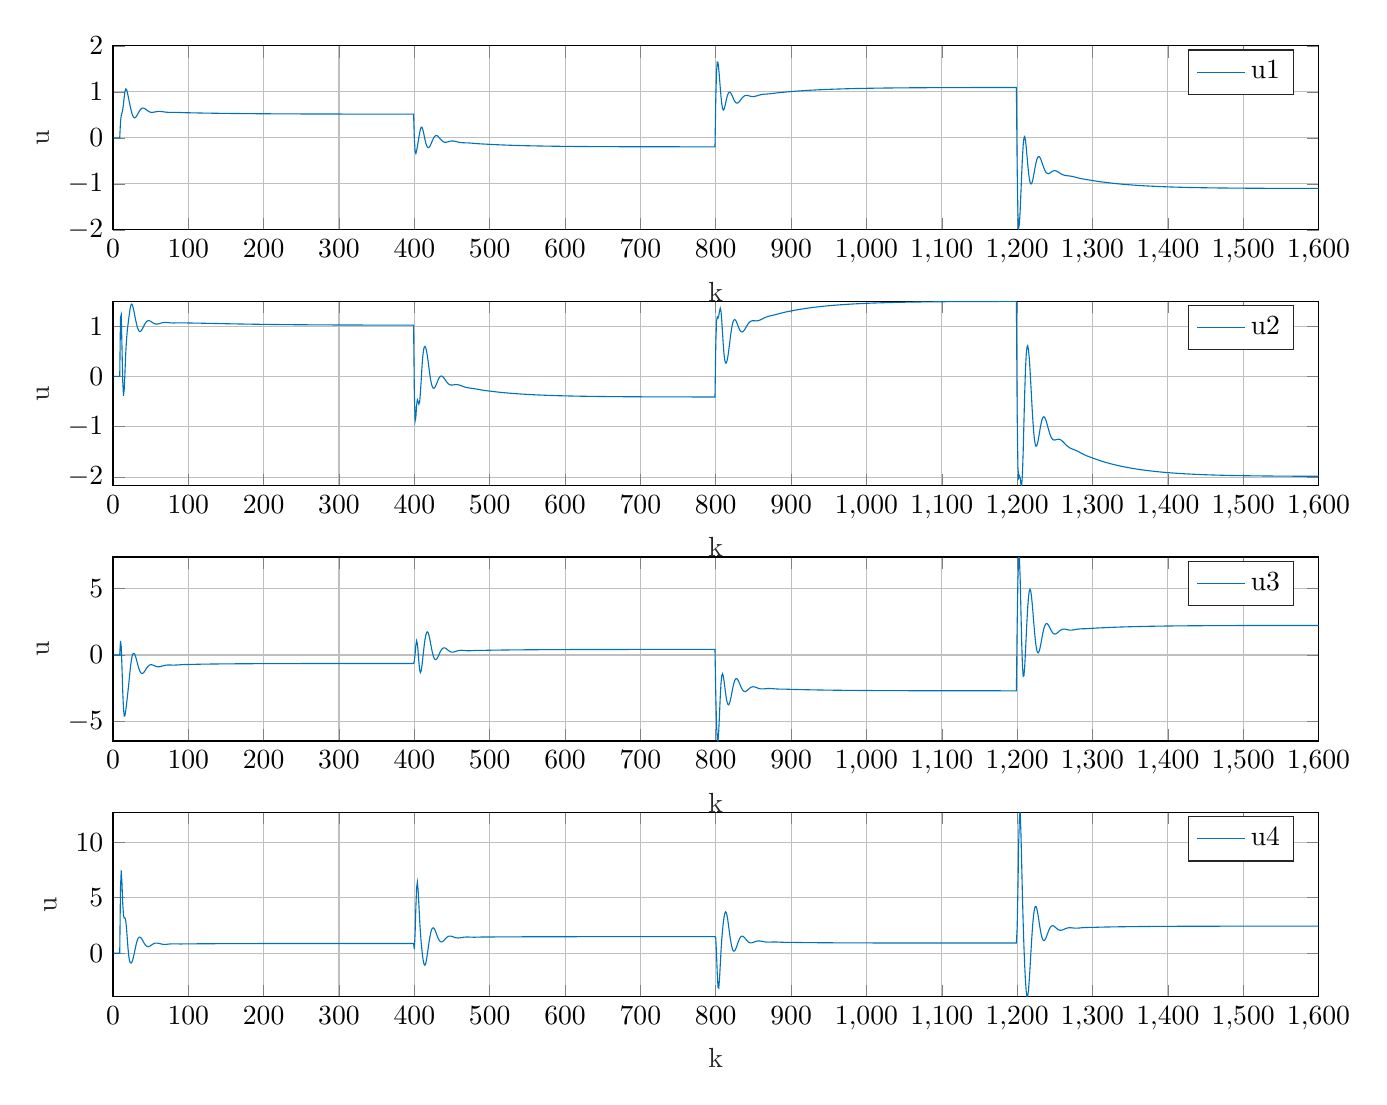
\begin{tikzpicture}

\begin{axis}[%
width=6.028in,
height=0.92in,
at={(1.011in,4.476in)},
scale only axis,
xmin=0,
xmax=1600,
xlabel style={font=\color{white!15!black}},
xlabel={k},
ymin=-2,
ymax=2,
ylabel style={font=\color{white!15!black}},
ylabel={u},
axis background/.style={fill=white},
xmajorgrids,
ymajorgrids,
legend style={legend cell align=left, align=left, draw=white!15!black}
]
\addplot [color=mycolor1]
  table[row sep=crcr]{%
1	0\\
2	0\\
3	0\\
4	0\\
5	0\\
6	0\\
7	0\\
8	0\\
9	0\\
10	0.3445\\
11	0.48802\\
12	0.54011\\
13	0.61399\\
14	0.74317\\
15	0.89261\\
16	1.0093\\
17	1.0619\\
18	1.0509\\
19	0.99615\\
20	0.92019\\
21	0.83811\\
22	0.75672\\
23	0.67853\\
24	0.60578\\
25	0.54193\\
26	0.49091\\
27	0.45561\\
28	0.43693\\
29	0.43376\\
30	0.44359\\
31	0.46327\\
32	0.48954\\
33	0.51932\\
34	0.54979\\
35	0.57853\\
36	0.60355\\
37	0.62343\\
38	0.63734\\
39	0.64508\\
40	0.64696\\
41	0.64369\\
42	0.6363\\
43	0.62593\\
44	0.61381\\
45	0.60108\\
46	0.58875\\
47	0.57764\\
48	0.56835\\
49	0.56124\\
50	0.55644\\
51	0.55387\\
52	0.55331\\
53	0.55438\\
54	0.55668\\
55	0.55975\\
56	0.56314\\
57	0.56647\\
58	0.56942\\
59	0.57173\\
60	0.57327\\
61	0.57397\\
62	0.57385\\
63	0.57299\\
64	0.5715\\
65	0.56956\\
66	0.56733\\
67	0.56497\\
68	0.56265\\
69	0.56048\\
70	0.55856\\
71	0.55696\\
72	0.55569\\
73	0.55476\\
74	0.55414\\
75	0.55378\\
76	0.55363\\
77	0.55361\\
78	0.55366\\
79	0.55373\\
80	0.55376\\
81	0.55372\\
82	0.55357\\
83	0.55332\\
84	0.55294\\
85	0.55246\\
86	0.5519\\
87	0.55126\\
88	0.55058\\
89	0.54988\\
90	0.54919\\
91	0.54851\\
92	0.54788\\
93	0.54729\\
94	0.54676\\
95	0.54628\\
96	0.54586\\
97	0.54547\\
98	0.54513\\
99	0.54481\\
100	0.54451\\
101	0.54422\\
102	0.54393\\
103	0.54363\\
104	0.54333\\
105	0.54301\\
106	0.54268\\
107	0.54234\\
108	0.54198\\
109	0.54162\\
110	0.54126\\
111	0.5409\\
112	0.54053\\
113	0.54018\\
114	0.53983\\
115	0.53949\\
116	0.53916\\
117	0.53885\\
118	0.53854\\
119	0.53825\\
120	0.53796\\
121	0.53768\\
122	0.5374\\
123	0.53713\\
124	0.53687\\
125	0.5366\\
126	0.53634\\
127	0.53608\\
128	0.53582\\
129	0.53555\\
130	0.53529\\
131	0.53503\\
132	0.53478\\
133	0.53452\\
134	0.53427\\
135	0.53402\\
136	0.53377\\
137	0.53353\\
138	0.53329\\
139	0.53306\\
140	0.53283\\
141	0.5326\\
142	0.53237\\
143	0.53215\\
144	0.53194\\
145	0.53172\\
146	0.53151\\
147	0.5313\\
148	0.53109\\
149	0.53088\\
150	0.53068\\
151	0.53047\\
152	0.53027\\
153	0.53008\\
154	0.52988\\
155	0.52969\\
156	0.52949\\
157	0.5293\\
158	0.52912\\
159	0.52893\\
160	0.52875\\
161	0.52857\\
162	0.52839\\
163	0.52821\\
164	0.52804\\
165	0.52786\\
166	0.52769\\
167	0.52753\\
168	0.52736\\
169	0.5272\\
170	0.52703\\
171	0.52687\\
172	0.52671\\
173	0.52656\\
174	0.5264\\
175	0.52625\\
176	0.5261\\
177	0.52595\\
178	0.5258\\
179	0.52565\\
180	0.52551\\
181	0.52536\\
182	0.52522\\
183	0.52508\\
184	0.52494\\
185	0.52481\\
186	0.52467\\
187	0.52454\\
188	0.52441\\
189	0.52428\\
190	0.52415\\
191	0.52402\\
192	0.5239\\
193	0.52377\\
194	0.52365\\
195	0.52353\\
196	0.52341\\
197	0.52329\\
198	0.52318\\
199	0.52306\\
200	0.52295\\
201	0.52284\\
202	0.52272\\
203	0.52261\\
204	0.52251\\
205	0.5224\\
206	0.52229\\
207	0.52219\\
208	0.52209\\
209	0.52198\\
210	0.52188\\
211	0.52178\\
212	0.52169\\
213	0.52159\\
214	0.52149\\
215	0.5214\\
216	0.52131\\
217	0.52121\\
218	0.52112\\
219	0.52103\\
220	0.52094\\
221	0.52086\\
222	0.52077\\
223	0.52068\\
224	0.5206\\
225	0.52052\\
226	0.52043\\
227	0.52035\\
228	0.52027\\
229	0.52019\\
230	0.52012\\
231	0.52004\\
232	0.51996\\
233	0.51989\\
234	0.51981\\
235	0.51974\\
236	0.51967\\
237	0.5196\\
238	0.51953\\
239	0.51946\\
240	0.51939\\
241	0.51932\\
242	0.51925\\
243	0.51919\\
244	0.51912\\
245	0.51906\\
246	0.519\\
247	0.51893\\
248	0.51887\\
249	0.51881\\
250	0.51875\\
251	0.51869\\
252	0.51863\\
253	0.51858\\
254	0.51852\\
255	0.51846\\
256	0.51841\\
257	0.51835\\
258	0.5183\\
259	0.51825\\
260	0.51819\\
261	0.51814\\
262	0.51809\\
263	0.51804\\
264	0.51799\\
265	0.51794\\
266	0.51789\\
267	0.51785\\
268	0.5178\\
269	0.51775\\
270	0.5177\\
271	0.51766\\
272	0.51761\\
273	0.51757\\
274	0.51752\\
275	0.51748\\
276	0.51744\\
277	0.5174\\
278	0.51736\\
279	0.51732\\
280	0.51728\\
281	0.51724\\
282	0.5172\\
283	0.51716\\
284	0.51712\\
285	0.51708\\
286	0.51705\\
287	0.51701\\
288	0.51697\\
289	0.51694\\
290	0.5169\\
291	0.51687\\
292	0.51683\\
293	0.5168\\
294	0.51677\\
295	0.51673\\
296	0.5167\\
297	0.51667\\
298	0.51664\\
299	0.51661\\
300	0.51658\\
301	0.51655\\
302	0.51652\\
303	0.51649\\
304	0.51646\\
305	0.51643\\
306	0.5164\\
307	0.51638\\
308	0.51635\\
309	0.51632\\
310	0.5163\\
311	0.51627\\
312	0.51625\\
313	0.51622\\
314	0.5162\\
315	0.51617\\
316	0.51615\\
317	0.51612\\
318	0.5161\\
319	0.51608\\
320	0.51606\\
321	0.51603\\
322	0.51601\\
323	0.51599\\
324	0.51597\\
325	0.51595\\
326	0.51593\\
327	0.51591\\
328	0.51589\\
329	0.51587\\
330	0.51585\\
331	0.51584\\
332	0.51582\\
333	0.5158\\
334	0.51578\\
335	0.51577\\
336	0.51575\\
337	0.51574\\
338	0.51572\\
339	0.5157\\
340	0.51569\\
341	0.51568\\
342	0.51566\\
343	0.51565\\
344	0.51564\\
345	0.51562\\
346	0.51561\\
347	0.5156\\
348	0.51559\\
349	0.51558\\
350	0.51557\\
351	0.51556\\
352	0.51555\\
353	0.51554\\
354	0.51554\\
355	0.51553\\
356	0.51552\\
357	0.51551\\
358	0.5155\\
359	0.51549\\
360	0.51548\\
361	0.51547\\
362	0.51545\\
363	0.51542\\
364	0.5154\\
365	0.51537\\
366	0.51534\\
367	0.51532\\
368	0.51529\\
369	0.51527\\
370	0.51525\\
371	0.51524\\
372	0.51523\\
373	0.51522\\
374	0.51522\\
375	0.51522\\
376	0.51523\\
377	0.51523\\
378	0.51523\\
379	0.51523\\
380	0.51523\\
381	0.51523\\
382	0.51522\\
383	0.51522\\
384	0.5152\\
385	0.51519\\
386	0.51517\\
387	0.51516\\
388	0.51514\\
389	0.51512\\
390	0.51511\\
391	0.5151\\
392	0.51508\\
393	0.51507\\
394	0.51506\\
395	0.51506\\
396	0.51505\\
397	0.51505\\
398	0.51505\\
399	0.51504\\
400	-0.030106\\
401	-0.29609\\
402	-0.34229\\
403	-0.28227\\
404	-0.19069\\
405	-0.092937\\
406	0.0076304\\
407	0.10511\\
408	0.18472\\
409	0.23007\\
410	0.2325\\
411	0.19485\\
412	0.12878\\
413	0.049203\\
414	-0.03054\\
415	-0.10092\\
416	-0.15627\\
417	-0.19381\\
418	-0.21277\\
419	-0.21393\\
420	-0.19938\\
421	-0.17239\\
422	-0.13698\\
423	-0.097451\\
424	-0.057901\\
425	-0.021802\\
426	0.0082166\\
427	0.03045\\
428	0.044098\\
429	0.049171\\
430	0.046364\\
431	0.036896\\
432	0.022341\\
433	0.0044436\\
434	-0.015044\\
435	-0.03451\\
436	-0.052589\\
437	-0.068235\\
438	-0.080756\\
439	-0.089811\\
440	-0.095385\\
441	-0.097735\\
442	-0.097332\\
443	-0.094787\\
444	-0.090782\\
445	-0.086006\\
446	-0.081096\\
447	-0.0766\\
448	-0.072943\\
449	-0.070416\\
450	-0.069171\\
451	-0.069236\\
452	-0.070528\\
453	-0.072878\\
454	-0.07606\\
455	-0.079817\\
456	-0.083883\\
457	-0.088013\\
458	-0.091989\\
459	-0.095643\\
460	-0.098855\\
461	-0.10156\\
462	-0.10373\\
463	-0.10541\\
464	-0.10665\\
465	-0.10753\\
466	-0.10814\\
467	-0.1086\\
468	-0.109\\
469	-0.10941\\
470	-0.10991\\
471	-0.11056\\
472	-0.11136\\
473	-0.11234\\
474	-0.11349\\
475	-0.11479\\
476	-0.1162\\
477	-0.1177\\
478	-0.11923\\
479	-0.12077\\
480	-0.12229\\
481	-0.12375\\
482	-0.12514\\
483	-0.12645\\
484	-0.12766\\
485	-0.12879\\
486	-0.12984\\
487	-0.13082\\
488	-0.13174\\
489	-0.13263\\
490	-0.13349\\
491	-0.13434\\
492	-0.13519\\
493	-0.13604\\
494	-0.13691\\
495	-0.13779\\
496	-0.13868\\
497	-0.13959\\
498	-0.1405\\
499	-0.14141\\
500	-0.14233\\
501	-0.14323\\
502	-0.14412\\
503	-0.145\\
504	-0.14585\\
505	-0.14668\\
506	-0.14749\\
507	-0.14828\\
508	-0.14905\\
509	-0.1498\\
510	-0.15053\\
511	-0.15124\\
512	-0.15194\\
513	-0.15263\\
514	-0.15331\\
515	-0.15398\\
516	-0.15465\\
517	-0.15531\\
518	-0.15596\\
519	-0.1566\\
520	-0.15724\\
521	-0.15788\\
522	-0.1585\\
523	-0.15912\\
524	-0.15972\\
525	-0.16032\\
526	-0.16091\\
527	-0.16148\\
528	-0.16205\\
529	-0.1626\\
530	-0.16315\\
531	-0.16368\\
532	-0.16421\\
533	-0.16473\\
534	-0.16524\\
535	-0.16574\\
536	-0.16623\\
537	-0.16672\\
538	-0.16719\\
539	-0.16767\\
540	-0.16813\\
541	-0.16859\\
542	-0.16904\\
543	-0.16948\\
544	-0.16992\\
545	-0.17035\\
546	-0.17078\\
547	-0.17119\\
548	-0.1716\\
549	-0.17201\\
550	-0.17241\\
551	-0.1728\\
552	-0.17318\\
553	-0.17356\\
554	-0.17393\\
555	-0.1743\\
556	-0.17466\\
557	-0.17501\\
558	-0.17536\\
559	-0.1757\\
560	-0.17604\\
561	-0.17637\\
562	-0.1767\\
563	-0.17702\\
564	-0.17734\\
565	-0.17765\\
566	-0.17795\\
567	-0.17826\\
568	-0.17855\\
569	-0.17885\\
570	-0.17913\\
571	-0.17942\\
572	-0.17969\\
573	-0.17997\\
574	-0.18024\\
575	-0.1805\\
576	-0.18076\\
577	-0.18102\\
578	-0.18127\\
579	-0.18152\\
580	-0.18176\\
581	-0.182\\
582	-0.18224\\
583	-0.18247\\
584	-0.1827\\
585	-0.18292\\
586	-0.18314\\
587	-0.18336\\
588	-0.18358\\
589	-0.18379\\
590	-0.18399\\
591	-0.1842\\
592	-0.1844\\
593	-0.18459\\
594	-0.18479\\
595	-0.18498\\
596	-0.18517\\
597	-0.18535\\
598	-0.18553\\
599	-0.18571\\
600	-0.18589\\
601	-0.18606\\
602	-0.18623\\
603	-0.1864\\
604	-0.18656\\
605	-0.18672\\
606	-0.18688\\
607	-0.18704\\
608	-0.18719\\
609	-0.18734\\
610	-0.18749\\
611	-0.18764\\
612	-0.18778\\
613	-0.18792\\
614	-0.18806\\
615	-0.1882\\
616	-0.18833\\
617	-0.18847\\
618	-0.1886\\
619	-0.18873\\
620	-0.18885\\
621	-0.18898\\
622	-0.1891\\
623	-0.18922\\
624	-0.18933\\
625	-0.18945\\
626	-0.18957\\
627	-0.18968\\
628	-0.18979\\
629	-0.1899\\
630	-0.19\\
631	-0.19011\\
632	-0.19021\\
633	-0.19031\\
634	-0.19041\\
635	-0.19051\\
636	-0.19061\\
637	-0.1907\\
638	-0.1908\\
639	-0.19089\\
640	-0.19098\\
641	-0.19107\\
642	-0.19115\\
643	-0.19124\\
644	-0.19132\\
645	-0.19141\\
646	-0.19149\\
647	-0.19157\\
648	-0.19165\\
649	-0.19173\\
650	-0.1918\\
651	-0.19188\\
652	-0.19195\\
653	-0.19202\\
654	-0.19209\\
655	-0.19216\\
656	-0.19223\\
657	-0.1923\\
658	-0.19237\\
659	-0.19243\\
660	-0.1925\\
661	-0.19256\\
662	-0.19262\\
663	-0.19269\\
664	-0.19275\\
665	-0.19281\\
666	-0.19286\\
667	-0.19292\\
668	-0.19298\\
669	-0.19303\\
670	-0.19309\\
671	-0.19314\\
672	-0.19319\\
673	-0.19324\\
674	-0.19329\\
675	-0.19334\\
676	-0.19339\\
677	-0.19344\\
678	-0.19349\\
679	-0.19354\\
680	-0.19358\\
681	-0.19363\\
682	-0.19367\\
683	-0.19372\\
684	-0.19376\\
685	-0.1938\\
686	-0.19384\\
687	-0.19389\\
688	-0.19393\\
689	-0.19397\\
690	-0.194\\
691	-0.19404\\
692	-0.19408\\
693	-0.19412\\
694	-0.19415\\
695	-0.19419\\
696	-0.19422\\
697	-0.19426\\
698	-0.19429\\
699	-0.19433\\
700	-0.19436\\
701	-0.19439\\
702	-0.19442\\
703	-0.19445\\
704	-0.19449\\
705	-0.19452\\
706	-0.19455\\
707	-0.19457\\
708	-0.1946\\
709	-0.19463\\
710	-0.19466\\
711	-0.19469\\
712	-0.19471\\
713	-0.19474\\
714	-0.19477\\
715	-0.19479\\
716	-0.19482\\
717	-0.19484\\
718	-0.19487\\
719	-0.19489\\
720	-0.19491\\
721	-0.19494\\
722	-0.19496\\
723	-0.19498\\
724	-0.19501\\
725	-0.19503\\
726	-0.19505\\
727	-0.19507\\
728	-0.19509\\
729	-0.19511\\
730	-0.19513\\
731	-0.19515\\
732	-0.19517\\
733	-0.19519\\
734	-0.19521\\
735	-0.19523\\
736	-0.19524\\
737	-0.19526\\
738	-0.19528\\
739	-0.1953\\
740	-0.19531\\
741	-0.19533\\
742	-0.19535\\
743	-0.19536\\
744	-0.19538\\
745	-0.19539\\
746	-0.19541\\
747	-0.19542\\
748	-0.19544\\
749	-0.19545\\
750	-0.19547\\
751	-0.19548\\
752	-0.19549\\
753	-0.19551\\
754	-0.19552\\
755	-0.19554\\
756	-0.19556\\
757	-0.19558\\
758	-0.19561\\
759	-0.19563\\
760	-0.19565\\
761	-0.19567\\
762	-0.19568\\
763	-0.19569\\
764	-0.19569\\
765	-0.1957\\
766	-0.19569\\
767	-0.19569\\
768	-0.19569\\
769	-0.19568\\
770	-0.19568\\
771	-0.19568\\
772	-0.19569\\
773	-0.1957\\
774	-0.19571\\
775	-0.19572\\
776	-0.19574\\
777	-0.19576\\
778	-0.19578\\
779	-0.19579\\
780	-0.19581\\
781	-0.19583\\
782	-0.19584\\
783	-0.19585\\
784	-0.19586\\
785	-0.19587\\
786	-0.19587\\
787	-0.19587\\
788	-0.19588\\
789	-0.19588\\
790	-0.19588\\
791	-0.19588\\
792	-0.19588\\
793	-0.19589\\
794	-0.19589\\
795	-0.1959\\
796	-0.1959\\
797	-0.19591\\
798	-0.19592\\
799	-0.19593\\
800	0.82817\\
801	1.4242\\
802	1.6471\\
803	1.6325\\
804	1.4929\\
805	1.2969\\
806	1.0857\\
807	0.88994\\
808	0.73519\\
809	0.63808\\
810	0.60249\\
811	0.6199\\
812	0.67407\\
813	0.7469\\
814	0.82281\\
815	0.89061\\
816	0.94348\\
817	0.97802\\
818	0.99342\\
819	0.99082\\
820	0.97296\\
821	0.9437\\
822	0.90755\\
823	0.86905\\
824	0.83233\\
825	0.80068\\
826	0.77644\\
827	0.76091\\
828	0.75443\\
829	0.75653\\
830	0.7661\\
831	0.78156\\
832	0.80108\\
833	0.82276\\
834	0.84482\\
835	0.86567\\
836	0.88411\\
837	0.89926\\
838	0.91066\\
839	0.91822\\
840	0.92214\\
841	0.9229\\
842	0.92113\\
843	0.91759\\
844	0.91303\\
845	0.90817\\
846	0.90364\\
847	0.89996\\
848	0.89746\\
849	0.89637\\
850	0.89674\\
851	0.89849\\
852	0.90148\\
853	0.90544\\
854	0.91012\\
855	0.9152\\
856	0.92041\\
857	0.9255\\
858	0.93026\\
859	0.93456\\
860	0.9383\\
861	0.94145\\
862	0.94403\\
863	0.94609\\
864	0.94773\\
865	0.94905\\
866	0.95016\\
867	0.95117\\
868	0.95218\\
869	0.95326\\
870	0.95448\\
871	0.95588\\
872	0.95746\\
873	0.95923\\
874	0.96116\\
875	0.96323\\
876	0.96539\\
877	0.96761\\
878	0.96983\\
879	0.97203\\
880	0.97418\\
881	0.97624\\
882	0.9782\\
883	0.98007\\
884	0.98183\\
885	0.98349\\
886	0.98507\\
887	0.98658\\
888	0.98804\\
889	0.98946\\
890	0.99086\\
891	0.99225\\
892	0.99365\\
893	0.99505\\
894	0.99646\\
895	0.99788\\
896	0.99931\\
897	1.0007\\
898	1.0022\\
899	1.0036\\
900	1.005\\
901	1.0064\\
902	1.0078\\
903	1.0091\\
904	1.0105\\
905	1.0118\\
906	1.013\\
907	1.0143\\
908	1.0155\\
909	1.0167\\
910	1.0178\\
911	1.019\\
912	1.0201\\
913	1.0212\\
914	1.0223\\
915	1.0234\\
916	1.0244\\
917	1.0255\\
918	1.0266\\
919	1.0276\\
920	1.0286\\
921	1.0296\\
922	1.0306\\
923	1.0316\\
924	1.0326\\
925	1.0336\\
926	1.0345\\
927	1.0354\\
928	1.0364\\
929	1.0373\\
930	1.0381\\
931	1.039\\
932	1.0399\\
933	1.0407\\
934	1.0415\\
935	1.0424\\
936	1.0432\\
937	1.044\\
938	1.0447\\
939	1.0455\\
940	1.0463\\
941	1.047\\
942	1.0478\\
943	1.0485\\
944	1.0492\\
945	1.0499\\
946	1.0506\\
947	1.0513\\
948	1.052\\
949	1.0527\\
950	1.0533\\
951	1.054\\
952	1.0546\\
953	1.0552\\
954	1.0558\\
955	1.0564\\
956	1.057\\
957	1.0576\\
958	1.0582\\
959	1.0588\\
960	1.0593\\
961	1.0599\\
962	1.0604\\
963	1.061\\
964	1.0615\\
965	1.062\\
966	1.0625\\
967	1.0631\\
968	1.0636\\
969	1.064\\
970	1.0645\\
971	1.065\\
972	1.0655\\
973	1.0659\\
974	1.0664\\
975	1.0668\\
976	1.0673\\
977	1.0677\\
978	1.0681\\
979	1.0685\\
980	1.069\\
981	1.0694\\
982	1.0698\\
983	1.0702\\
984	1.0706\\
985	1.0709\\
986	1.0713\\
987	1.0717\\
988	1.072\\
989	1.0724\\
990	1.0728\\
991	1.0731\\
992	1.0734\\
993	1.0738\\
994	1.0741\\
995	1.0744\\
996	1.0748\\
997	1.0751\\
998	1.0754\\
999	1.0757\\
1000	1.076\\
1001	1.0763\\
1002	1.0766\\
1003	1.0769\\
1004	1.0772\\
1005	1.0774\\
1006	1.0777\\
1007	1.078\\
1008	1.0783\\
1009	1.0785\\
1010	1.0788\\
1011	1.079\\
1012	1.0793\\
1013	1.0795\\
1014	1.0798\\
1015	1.08\\
1016	1.0802\\
1017	1.0805\\
1018	1.0807\\
1019	1.0809\\
1020	1.0811\\
1021	1.0813\\
1022	1.0816\\
1023	1.0818\\
1024	1.082\\
1025	1.0822\\
1026	1.0824\\
1027	1.0826\\
1028	1.0828\\
1029	1.083\\
1030	1.0831\\
1031	1.0833\\
1032	1.0835\\
1033	1.0837\\
1034	1.0839\\
1035	1.084\\
1036	1.0842\\
1037	1.0844\\
1038	1.0845\\
1039	1.0847\\
1040	1.0849\\
1041	1.085\\
1042	1.0852\\
1043	1.0853\\
1044	1.0855\\
1045	1.0856\\
1046	1.0858\\
1047	1.0859\\
1048	1.086\\
1049	1.0862\\
1050	1.0863\\
1051	1.0865\\
1052	1.0866\\
1053	1.0867\\
1054	1.0868\\
1055	1.087\\
1056	1.0871\\
1057	1.0872\\
1058	1.0873\\
1059	1.0874\\
1060	1.0876\\
1061	1.0877\\
1062	1.0878\\
1063	1.0879\\
1064	1.088\\
1065	1.0881\\
1066	1.0882\\
1067	1.0883\\
1068	1.0884\\
1069	1.0885\\
1070	1.0886\\
1071	1.0887\\
1072	1.0888\\
1073	1.0889\\
1074	1.089\\
1075	1.0891\\
1076	1.0892\\
1077	1.0892\\
1078	1.0893\\
1079	1.0894\\
1080	1.0895\\
1081	1.0896\\
1082	1.0897\\
1083	1.0897\\
1084	1.0898\\
1085	1.0899\\
1086	1.09\\
1087	1.09\\
1088	1.0901\\
1089	1.0902\\
1090	1.0903\\
1091	1.0903\\
1092	1.0904\\
1093	1.0905\\
1094	1.0905\\
1095	1.0906\\
1096	1.0907\\
1097	1.0907\\
1098	1.0908\\
1099	1.0908\\
1100	1.0909\\
1101	1.091\\
1102	1.091\\
1103	1.0911\\
1104	1.0911\\
1105	1.0912\\
1106	1.0912\\
1107	1.0913\\
1108	1.0914\\
1109	1.0914\\
1110	1.0915\\
1111	1.0915\\
1112	1.0916\\
1113	1.0916\\
1114	1.0917\\
1115	1.0917\\
1116	1.0917\\
1117	1.0918\\
1118	1.0918\\
1119	1.0919\\
1120	1.0919\\
1121	1.092\\
1122	1.092\\
1123	1.0921\\
1124	1.0921\\
1125	1.0921\\
1126	1.0922\\
1127	1.0922\\
1128	1.0923\\
1129	1.0923\\
1130	1.0923\\
1131	1.0924\\
1132	1.0924\\
1133	1.0924\\
1134	1.0925\\
1135	1.0925\\
1136	1.0925\\
1137	1.0926\\
1138	1.0926\\
1139	1.0926\\
1140	1.0927\\
1141	1.0927\\
1142	1.0927\\
1143	1.0928\\
1144	1.0928\\
1145	1.0928\\
1146	1.0929\\
1147	1.0929\\
1148	1.0929\\
1149	1.0929\\
1150	1.093\\
1151	1.093\\
1152	1.093\\
1153	1.093\\
1154	1.0931\\
1155	1.0931\\
1156	1.0931\\
1157	1.0932\\
1158	1.0932\\
1159	1.0932\\
1160	1.0933\\
1161	1.0933\\
1162	1.0933\\
1163	1.0933\\
1164	1.0933\\
1165	1.0933\\
1166	1.0933\\
1167	1.0933\\
1168	1.0934\\
1169	1.0934\\
1170	1.0934\\
1171	1.0934\\
1172	1.0934\\
1173	1.0934\\
1174	1.0934\\
1175	1.0935\\
1176	1.0935\\
1177	1.0935\\
1178	1.0935\\
1179	1.0936\\
1180	1.0936\\
1181	1.0936\\
1182	1.0936\\
1183	1.0936\\
1184	1.0937\\
1185	1.0937\\
1186	1.0937\\
1187	1.0937\\
1188	1.0937\\
1189	1.0937\\
1190	1.0937\\
1191	1.0937\\
1192	1.0937\\
1193	1.0937\\
1194	1.0938\\
1195	1.0938\\
1196	1.0938\\
1197	1.0938\\
1198	1.0938\\
1199	1.0938\\
1200	-0.6504\\
1201	-1.6384\\
1202	-1.9643\\
1203	-1.8751\\
1204	-1.5757\\
1205	-1.1895\\
1206	-0.78916\\
1207	-0.42953\\
1208	-0.15721\\
1209	-0.0029819\\
1210	0.026814\\
1211	-0.04991\\
1212	-0.19969\\
1213	-0.38504\\
1214	-0.57322\\
1215	-0.74031\\
1216	-0.87131\\
1217	-0.95857\\
1218	-1.0001\\
1219	-0.99838\\
1220	-0.95953\\
1221	-0.89233\\
1222	-0.80706\\
1223	-0.71428\\
1224	-0.62369\\
1225	-0.5433\\
1226	-0.47896\\
1227	-0.43421\\
1228	-0.41041\\
1229	-0.40698\\
1230	-0.42174\\
1231	-0.45136\\
1232	-0.4918\\
1233	-0.53872\\
1234	-0.58792\\
1235	-0.63566\\
1236	-0.67886\\
1237	-0.71528\\
1238	-0.74355\\
1239	-0.76317\\
1240	-0.77437\\
1241	-0.77802\\
1242	-0.77545\\
1243	-0.76825\\
1244	-0.75815\\
1245	-0.74679\\
1246	-0.7357\\
1247	-0.72609\\
1248	-0.7189\\
1249	-0.71471\\
1250	-0.71376\\
1251	-0.716\\
1252	-0.72113\\
1253	-0.72867\\
1254	-0.73802\\
1255	-0.74852\\
1256	-0.75953\\
1257	-0.77046\\
1258	-0.78082\\
1259	-0.79023\\
1260	-0.79846\\
1261	-0.80539\\
1262	-0.81101\\
1263	-0.81544\\
1264	-0.81884\\
1265	-0.82145\\
1266	-0.8235\\
1267	-0.82525\\
1268	-0.82692\\
1269	-0.82871\\
1270	-0.83076\\
1271	-0.83319\\
1272	-0.83603\\
1273	-0.8393\\
1274	-0.84297\\
1275	-0.84696\\
1276	-0.85121\\
1277	-0.85561\\
1278	-0.86008\\
1279	-0.86451\\
1280	-0.86885\\
1281	-0.87303\\
1282	-0.877\\
1283	-0.88076\\
1284	-0.88429\\
1285	-0.8876\\
1286	-0.89072\\
1287	-0.89367\\
1288	-0.8965\\
1289	-0.89924\\
1290	-0.90193\\
1291	-0.90459\\
1292	-0.90725\\
1293	-0.90993\\
1294	-0.91263\\
1295	-0.91536\\
1296	-0.91813\\
1297	-0.92091\\
1298	-0.92369\\
1299	-0.92648\\
1300	-0.92925\\
1301	-0.93198\\
1302	-0.93468\\
1303	-0.93732\\
1304	-0.93991\\
1305	-0.94244\\
1306	-0.94491\\
1307	-0.94731\\
1308	-0.94966\\
1309	-0.95196\\
1310	-0.95421\\
1311	-0.95642\\
1312	-0.9586\\
1313	-0.96074\\
1314	-0.96286\\
1315	-0.96495\\
1316	-0.96702\\
1317	-0.96908\\
1318	-0.97111\\
1319	-0.97312\\
1320	-0.97511\\
1321	-0.97707\\
1322	-0.97901\\
1323	-0.98093\\
1324	-0.98281\\
1325	-0.98467\\
1326	-0.9865\\
1327	-0.9883\\
1328	-0.99006\\
1329	-0.9918\\
1330	-0.99351\\
1331	-0.99519\\
1332	-0.99684\\
1333	-0.99847\\
1334	-1.0001\\
1335	-1.0016\\
1336	-1.0032\\
1337	-1.0047\\
1338	-1.0062\\
1339	-1.0077\\
1340	-1.0092\\
1341	-1.0107\\
1342	-1.0121\\
1343	-1.0135\\
1344	-1.0149\\
1345	-1.0162\\
1346	-1.0176\\
1347	-1.0189\\
1348	-1.0202\\
1349	-1.0215\\
1350	-1.0228\\
1351	-1.024\\
1352	-1.0252\\
1353	-1.0265\\
1354	-1.0276\\
1355	-1.0288\\
1356	-1.03\\
1357	-1.0311\\
1358	-1.0322\\
1359	-1.0333\\
1360	-1.0344\\
1361	-1.0355\\
1362	-1.0365\\
1363	-1.0376\\
1364	-1.0386\\
1365	-1.0396\\
1366	-1.0406\\
1367	-1.0415\\
1368	-1.0425\\
1369	-1.0434\\
1370	-1.0444\\
1371	-1.0453\\
1372	-1.0462\\
1373	-1.0471\\
1374	-1.0479\\
1375	-1.0488\\
1376	-1.0497\\
1377	-1.0505\\
1378	-1.0513\\
1379	-1.0521\\
1380	-1.0529\\
1381	-1.0537\\
1382	-1.0545\\
1383	-1.0552\\
1384	-1.056\\
1385	-1.0567\\
1386	-1.0574\\
1387	-1.0581\\
1388	-1.0588\\
1389	-1.0595\\
1390	-1.0602\\
1391	-1.0609\\
1392	-1.0615\\
1393	-1.0622\\
1394	-1.0628\\
1395	-1.0634\\
1396	-1.0641\\
1397	-1.0647\\
1398	-1.0653\\
1399	-1.0659\\
1400	-1.0664\\
1401	-1.067\\
1402	-1.0676\\
1403	-1.0681\\
1404	-1.0687\\
1405	-1.0692\\
1406	-1.0697\\
1407	-1.0703\\
1408	-1.0708\\
1409	-1.0713\\
1410	-1.0718\\
1411	-1.0723\\
1412	-1.0727\\
1413	-1.0732\\
1414	-1.0737\\
1415	-1.0741\\
1416	-1.0746\\
1417	-1.075\\
1418	-1.0755\\
1419	-1.0759\\
1420	-1.0763\\
1421	-1.0767\\
1422	-1.0771\\
1423	-1.0775\\
1424	-1.0779\\
1425	-1.0783\\
1426	-1.0787\\
1427	-1.0791\\
1428	-1.0795\\
1429	-1.0798\\
1430	-1.0802\\
1431	-1.0805\\
1432	-1.0809\\
1433	-1.0812\\
1434	-1.0816\\
1435	-1.0819\\
1436	-1.0822\\
1437	-1.0825\\
1438	-1.0829\\
1439	-1.0832\\
1440	-1.0835\\
1441	-1.0838\\
1442	-1.0841\\
1443	-1.0844\\
1444	-1.0847\\
1445	-1.0849\\
1446	-1.0852\\
1447	-1.0855\\
1448	-1.0858\\
1449	-1.086\\
1450	-1.0863\\
1451	-1.0865\\
1452	-1.0868\\
1453	-1.087\\
1454	-1.0873\\
1455	-1.0875\\
1456	-1.0878\\
1457	-1.088\\
1458	-1.0882\\
1459	-1.0884\\
1460	-1.0887\\
1461	-1.0889\\
1462	-1.0891\\
1463	-1.0893\\
1464	-1.0895\\
1465	-1.0897\\
1466	-1.0899\\
1467	-1.0901\\
1468	-1.0903\\
1469	-1.0905\\
1470	-1.0907\\
1471	-1.0909\\
1472	-1.0911\\
1473	-1.0912\\
1474	-1.0914\\
1475	-1.0916\\
1476	-1.0917\\
1477	-1.0919\\
1478	-1.0921\\
1479	-1.0922\\
1480	-1.0924\\
1481	-1.0926\\
1482	-1.0927\\
1483	-1.0929\\
1484	-1.093\\
1485	-1.0932\\
1486	-1.0933\\
1487	-1.0935\\
1488	-1.0936\\
1489	-1.0937\\
1490	-1.0939\\
1491	-1.094\\
1492	-1.0941\\
1493	-1.0943\\
1494	-1.0944\\
1495	-1.0945\\
1496	-1.0946\\
1497	-1.0948\\
1498	-1.0949\\
1499	-1.095\\
1500	-1.0951\\
1501	-1.0952\\
1502	-1.0953\\
1503	-1.0954\\
1504	-1.0956\\
1505	-1.0957\\
1506	-1.0958\\
1507	-1.0959\\
1508	-1.096\\
1509	-1.0961\\
1510	-1.0962\\
1511	-1.0963\\
1512	-1.0964\\
1513	-1.0965\\
1514	-1.0965\\
1515	-1.0966\\
1516	-1.0967\\
1517	-1.0968\\
1518	-1.0969\\
1519	-1.097\\
1520	-1.0971\\
1521	-1.0971\\
1522	-1.0972\\
1523	-1.0973\\
1524	-1.0974\\
1525	-1.0975\\
1526	-1.0975\\
1527	-1.0976\\
1528	-1.0977\\
1529	-1.0978\\
1530	-1.0978\\
1531	-1.0979\\
1532	-1.098\\
1533	-1.098\\
1534	-1.0981\\
1535	-1.0982\\
1536	-1.0982\\
1537	-1.0983\\
1538	-1.0984\\
1539	-1.0984\\
1540	-1.0985\\
1541	-1.0985\\
1542	-1.0986\\
1543	-1.0986\\
1544	-1.0987\\
1545	-1.0988\\
1546	-1.0988\\
1547	-1.0989\\
1548	-1.0989\\
1549	-1.099\\
1550	-1.099\\
1551	-1.0991\\
1552	-1.0991\\
1553	-1.0992\\
1554	-1.0992\\
1555	-1.0993\\
1556	-1.0994\\
1557	-1.0994\\
1558	-1.0995\\
1559	-1.0996\\
1560	-1.0996\\
1561	-1.0997\\
1562	-1.0997\\
1563	-1.0998\\
1564	-1.0998\\
1565	-1.0998\\
1566	-1.0998\\
1567	-1.0998\\
1568	-1.0998\\
1569	-1.0998\\
1570	-1.0998\\
1571	-1.0998\\
1572	-1.0999\\
1573	-1.0999\\
1574	-1.0999\\
1575	-1.1\\
1576	-1.1\\
1577	-1.1001\\
1578	-1.1002\\
1579	-1.1002\\
1580	-1.1003\\
1581	-1.1003\\
1582	-1.1003\\
1583	-1.1004\\
1584	-1.1004\\
1585	-1.1004\\
1586	-1.1004\\
1587	-1.1005\\
1588	-1.1005\\
1589	-1.1005\\
1590	-1.1005\\
1591	-1.1005\\
1592	-1.1005\\
1593	-1.1005\\
1594	-1.1006\\
1595	-1.1006\\
1596	-1.1006\\
1597	-1.1006\\
1598	-1.1007\\
1599	-1.1007\\
1600	-1.1007\\
};
\addlegendentry{u1}

\end{axis}

\begin{axis}[%
width=6.028in,
height=0.92in,
at={(1.011in,3.198in)},
scale only axis,
xmin=0,
xmax=1600,
xlabel style={font=\color{white!15!black}},
xlabel={k},
ymin=-2.1651,
ymax=1.4903,
ylabel style={font=\color{white!15!black}},
ylabel={u},
axis background/.style={fill=white},
xmajorgrids,
ymajorgrids,
legend style={legend cell align=left, align=left, draw=white!15!black}
]
\addplot [color=mycolor1]
  table[row sep=crcr]{%
1	0\\
2	0\\
3	0\\
4	0\\
5	0\\
6	0\\
7	0\\
8	0\\
9	0\\
10	1.1665\\
11	1.2245\\
12	0.57599\\
13	-0.10025\\
14	-0.38634\\
15	-0.25265\\
16	0.10184\\
17	0.46537\\
18	0.73278\\
19	0.90605\\
20	1.0333\\
21	1.1521\\
22	1.2683\\
23	1.3652\\
24	1.4242\\
25	1.4374\\
26	1.41\\
27	1.3543\\
28	1.2832\\
29	1.2065\\
30	1.1309\\
31	1.0608\\
32	0.99981\\
33	0.95099\\
34	0.91655\\
35	0.89737\\
36	0.89282\\
37	0.90102\\
38	0.91926\\
39	0.94447\\
40	0.9736\\
41	1.0038\\
42	1.0327\\
43	1.0583\\
44	1.0792\\
45	1.0946\\
46	1.1042\\
47	1.1082\\
48	1.1074\\
49	1.1025\\
50	1.0948\\
51	1.0853\\
52	1.0752\\
53	1.0653\\
54	1.0565\\
55	1.0494\\
56	1.0443\\
57	1.0413\\
58	1.0404\\
59	1.0413\\
60	1.0437\\
61	1.0472\\
62	1.0514\\
63	1.0559\\
64	1.0603\\
65	1.0642\\
66	1.0675\\
67	1.0701\\
68	1.0717\\
69	1.0725\\
70	1.0726\\
71	1.0721\\
72	1.071\\
73	1.0697\\
74	1.0682\\
75	1.0667\\
76	1.0653\\
77	1.0641\\
78	1.0632\\
79	1.0625\\
80	1.0622\\
81	1.0621\\
82	1.0623\\
83	1.0626\\
84	1.0631\\
85	1.0636\\
86	1.0641\\
87	1.0645\\
88	1.0648\\
89	1.0651\\
90	1.0651\\
91	1.0651\\
92	1.065\\
93	1.0647\\
94	1.0644\\
95	1.064\\
96	1.0635\\
97	1.0631\\
98	1.0626\\
99	1.0622\\
100	1.0618\\
101	1.0615\\
102	1.0612\\
103	1.0609\\
104	1.0607\\
105	1.0605\\
106	1.0603\\
107	1.0601\\
108	1.0599\\
109	1.0597\\
110	1.0595\\
111	1.0593\\
112	1.059\\
113	1.0588\\
114	1.0585\\
115	1.0582\\
116	1.0578\\
117	1.0575\\
118	1.0572\\
119	1.0568\\
120	1.0565\\
121	1.0562\\
122	1.0558\\
123	1.0555\\
124	1.0552\\
125	1.0549\\
126	1.0546\\
127	1.0542\\
128	1.0539\\
129	1.0536\\
130	1.0533\\
131	1.053\\
132	1.0527\\
133	1.0524\\
134	1.0521\\
135	1.0518\\
136	1.0515\\
137	1.0512\\
138	1.0508\\
139	1.0505\\
140	1.0502\\
141	1.0499\\
142	1.0496\\
143	1.0493\\
144	1.049\\
145	1.0486\\
146	1.0483\\
147	1.048\\
148	1.0477\\
149	1.0474\\
150	1.0471\\
151	1.0468\\
152	1.0465\\
153	1.0462\\
154	1.0459\\
155	1.0456\\
156	1.0453\\
157	1.045\\
158	1.0448\\
159	1.0445\\
160	1.0442\\
161	1.0439\\
162	1.0436\\
163	1.0433\\
164	1.0431\\
165	1.0428\\
166	1.0425\\
167	1.0422\\
168	1.042\\
169	1.0417\\
170	1.0414\\
171	1.0412\\
172	1.0409\\
173	1.0406\\
174	1.0404\\
175	1.0401\\
176	1.0399\\
177	1.0396\\
178	1.0393\\
179	1.0391\\
180	1.0389\\
181	1.0386\\
182	1.0384\\
183	1.0381\\
184	1.0379\\
185	1.0376\\
186	1.0374\\
187	1.0372\\
188	1.0369\\
189	1.0367\\
190	1.0365\\
191	1.0363\\
192	1.036\\
193	1.0358\\
194	1.0356\\
195	1.0354\\
196	1.0352\\
197	1.035\\
198	1.0348\\
199	1.0346\\
200	1.0343\\
201	1.0341\\
202	1.0339\\
203	1.0337\\
204	1.0335\\
205	1.0333\\
206	1.0332\\
207	1.033\\
208	1.0328\\
209	1.0326\\
210	1.0324\\
211	1.0322\\
212	1.032\\
213	1.0319\\
214	1.0317\\
215	1.0315\\
216	1.0313\\
217	1.0312\\
218	1.031\\
219	1.0308\\
220	1.0307\\
221	1.0305\\
222	1.0303\\
223	1.0302\\
224	1.03\\
225	1.0299\\
226	1.0297\\
227	1.0295\\
228	1.0294\\
229	1.0292\\
230	1.0291\\
231	1.0289\\
232	1.0288\\
233	1.0287\\
234	1.0285\\
235	1.0284\\
236	1.0282\\
237	1.0281\\
238	1.028\\
239	1.0278\\
240	1.0277\\
241	1.0276\\
242	1.0274\\
243	1.0273\\
244	1.0272\\
245	1.0271\\
246	1.0269\\
247	1.0268\\
248	1.0267\\
249	1.0266\\
250	1.0265\\
251	1.0264\\
252	1.0262\\
253	1.0261\\
254	1.026\\
255	1.0259\\
256	1.0258\\
257	1.0257\\
258	1.0256\\
259	1.0255\\
260	1.0254\\
261	1.0253\\
262	1.0252\\
263	1.0251\\
264	1.025\\
265	1.0249\\
266	1.0248\\
267	1.0247\\
268	1.0246\\
269	1.0245\\
270	1.0244\\
271	1.0243\\
272	1.0243\\
273	1.0242\\
274	1.0241\\
275	1.024\\
276	1.0239\\
277	1.0238\\
278	1.0238\\
279	1.0237\\
280	1.0236\\
281	1.0235\\
282	1.0234\\
283	1.0234\\
284	1.0233\\
285	1.0232\\
286	1.0231\\
287	1.0231\\
288	1.023\\
289	1.0229\\
290	1.0228\\
291	1.0228\\
292	1.0227\\
293	1.0226\\
294	1.0226\\
295	1.0225\\
296	1.0224\\
297	1.0224\\
298	1.0223\\
299	1.0223\\
300	1.0222\\
301	1.0221\\
302	1.0221\\
303	1.022\\
304	1.022\\
305	1.0219\\
306	1.0218\\
307	1.0218\\
308	1.0217\\
309	1.0217\\
310	1.0216\\
311	1.0216\\
312	1.0215\\
313	1.0215\\
314	1.0214\\
315	1.0214\\
316	1.0213\\
317	1.0213\\
318	1.0212\\
319	1.0212\\
320	1.0211\\
321	1.0211\\
322	1.021\\
323	1.021\\
324	1.021\\
325	1.0209\\
326	1.0209\\
327	1.0208\\
328	1.0208\\
329	1.0208\\
330	1.0207\\
331	1.0207\\
332	1.0206\\
333	1.0206\\
334	1.0206\\
335	1.0205\\
336	1.0205\\
337	1.0205\\
338	1.0204\\
339	1.0204\\
340	1.0204\\
341	1.0203\\
342	1.0203\\
343	1.0203\\
344	1.0202\\
345	1.0202\\
346	1.0202\\
347	1.0202\\
348	1.0201\\
349	1.0201\\
350	1.0201\\
351	1.02\\
352	1.02\\
353	1.02\\
354	1.02\\
355	1.0199\\
356	1.0199\\
357	1.0199\\
358	1.0199\\
359	1.0199\\
360	1.0198\\
361	1.0198\\
362	1.0198\\
363	1.0198\\
364	1.0198\\
365	1.0198\\
366	1.0198\\
367	1.0197\\
368	1.0197\\
369	1.0197\\
370	1.0196\\
371	1.0196\\
372	1.0196\\
373	1.0195\\
374	1.0195\\
375	1.0194\\
376	1.0194\\
377	1.0194\\
378	1.0193\\
379	1.0193\\
380	1.0193\\
381	1.0193\\
382	1.0193\\
383	1.0193\\
384	1.0193\\
385	1.0193\\
386	1.0193\\
387	1.0193\\
388	1.0193\\
389	1.0193\\
390	1.0192\\
391	1.0192\\
392	1.0192\\
393	1.0192\\
394	1.0191\\
395	1.0191\\
396	1.0191\\
397	1.0191\\
398	1.0191\\
399	1.019\\
400	-0.35646\\
401	-0.88682\\
402	-0.80781\\
403	-0.57277\\
404	-0.46222\\
405	-0.49593\\
406	-0.55002\\
407	-0.50854\\
408	-0.34098\\
409	-0.093548\\
410	0.16123\\
411	0.3684\\
412	0.50614\\
413	0.57786\\
414	0.59657\\
415	0.57389\\
416	0.51739\\
417	0.43304\\
418	0.3282\\
419	0.21258\\
420	0.09693\\
421	-0.0089501\\
422	-0.097806\\
423	-0.16543\\
424	-0.21037\\
425	-0.23331\\
426	-0.23644\\
427	-0.22306\\
428	-0.19715\\
429	-0.1631\\
430	-0.12528\\
431	-0.087728\\
432	-0.053845\\
433	-0.02619\\
434	-0.0064049\\
435	0.0047637\\
436	0.0073761\\
437	0.0021618\\
438	-0.0096436\\
439	-0.026475\\
440	-0.046609\\
441	-0.068328\\
442	-0.090051\\
443	-0.11044\\
444	-0.12847\\
445	-0.14347\\
446	-0.15508\\
447	-0.16328\\
448	-0.16832\\
449	-0.17064\\
450	-0.17083\\
451	-0.16955\\
452	-0.16745\\
453	-0.16516\\
454	-0.1632\\
455	-0.16198\\
456	-0.16179\\
457	-0.16278\\
458	-0.16498\\
459	-0.16831\\
460	-0.17261\\
461	-0.17768\\
462	-0.18326\\
463	-0.18911\\
464	-0.19498\\
465	-0.20067\\
466	-0.20602\\
467	-0.21092\\
468	-0.2153\\
469	-0.21914\\
470	-0.22247\\
471	-0.22534\\
472	-0.22785\\
473	-0.23007\\
474	-0.2321\\
475	-0.23405\\
476	-0.23599\\
477	-0.23798\\
478	-0.24008\\
479	-0.24231\\
480	-0.24468\\
481	-0.24718\\
482	-0.24981\\
483	-0.25252\\
484	-0.25528\\
485	-0.25807\\
486	-0.26083\\
487	-0.26355\\
488	-0.2662\\
489	-0.26875\\
490	-0.27121\\
491	-0.27355\\
492	-0.2758\\
493	-0.27794\\
494	-0.28\\
495	-0.28199\\
496	-0.28393\\
497	-0.28582\\
498	-0.28768\\
499	-0.28952\\
500	-0.29134\\
501	-0.29317\\
502	-0.29498\\
503	-0.2968\\
504	-0.29861\\
505	-0.30041\\
506	-0.3022\\
507	-0.30397\\
508	-0.30572\\
509	-0.30744\\
510	-0.30913\\
511	-0.31079\\
512	-0.31241\\
513	-0.31399\\
514	-0.31555\\
515	-0.31706\\
516	-0.31855\\
517	-0.32\\
518	-0.32143\\
519	-0.32283\\
520	-0.32421\\
521	-0.32557\\
522	-0.32691\\
523	-0.32823\\
524	-0.32954\\
525	-0.33082\\
526	-0.33209\\
527	-0.33334\\
528	-0.33458\\
529	-0.3358\\
530	-0.33699\\
531	-0.33817\\
532	-0.33933\\
533	-0.34047\\
534	-0.34159\\
535	-0.3427\\
536	-0.34378\\
537	-0.34484\\
538	-0.34589\\
539	-0.34692\\
540	-0.34793\\
541	-0.34892\\
542	-0.3499\\
543	-0.35086\\
544	-0.35181\\
545	-0.35274\\
546	-0.35366\\
547	-0.35456\\
548	-0.35545\\
549	-0.35632\\
550	-0.35718\\
551	-0.35803\\
552	-0.35887\\
553	-0.35969\\
554	-0.3605\\
555	-0.36129\\
556	-0.36207\\
557	-0.36284\\
558	-0.3636\\
559	-0.36434\\
560	-0.36507\\
561	-0.36579\\
562	-0.3665\\
563	-0.36719\\
564	-0.36788\\
565	-0.36855\\
566	-0.36922\\
567	-0.36987\\
568	-0.37051\\
569	-0.37114\\
570	-0.37176\\
571	-0.37237\\
572	-0.37297\\
573	-0.37356\\
574	-0.37415\\
575	-0.37472\\
576	-0.37528\\
577	-0.37584\\
578	-0.37638\\
579	-0.37692\\
580	-0.37744\\
581	-0.37796\\
582	-0.37847\\
583	-0.37897\\
584	-0.37947\\
585	-0.37995\\
586	-0.38043\\
587	-0.3809\\
588	-0.38136\\
589	-0.38182\\
590	-0.38226\\
591	-0.3827\\
592	-0.38314\\
593	-0.38356\\
594	-0.38398\\
595	-0.38439\\
596	-0.3848\\
597	-0.3852\\
598	-0.38559\\
599	-0.38597\\
600	-0.38635\\
601	-0.38673\\
602	-0.38709\\
603	-0.38745\\
604	-0.38781\\
605	-0.38816\\
606	-0.3885\\
607	-0.38884\\
608	-0.38917\\
609	-0.3895\\
610	-0.38982\\
611	-0.39014\\
612	-0.39045\\
613	-0.39075\\
614	-0.39105\\
615	-0.39135\\
616	-0.39164\\
617	-0.39193\\
618	-0.39221\\
619	-0.39248\\
620	-0.39276\\
621	-0.39302\\
622	-0.39329\\
623	-0.39355\\
624	-0.3938\\
625	-0.39405\\
626	-0.3943\\
627	-0.39454\\
628	-0.39478\\
629	-0.39501\\
630	-0.39524\\
631	-0.39547\\
632	-0.39569\\
633	-0.39591\\
634	-0.39613\\
635	-0.39634\\
636	-0.39655\\
637	-0.39676\\
638	-0.39696\\
639	-0.39716\\
640	-0.39735\\
641	-0.39754\\
642	-0.39773\\
643	-0.39792\\
644	-0.3981\\
645	-0.39828\\
646	-0.39846\\
647	-0.39863\\
648	-0.3988\\
649	-0.39897\\
650	-0.39913\\
651	-0.3993\\
652	-0.39946\\
653	-0.39961\\
654	-0.39977\\
655	-0.39992\\
656	-0.40007\\
657	-0.40021\\
658	-0.40036\\
659	-0.4005\\
660	-0.40063\\
661	-0.40077\\
662	-0.40091\\
663	-0.40104\\
664	-0.40117\\
665	-0.4013\\
666	-0.40143\\
667	-0.40155\\
668	-0.40167\\
669	-0.4018\\
670	-0.40191\\
671	-0.40203\\
672	-0.40215\\
673	-0.40226\\
674	-0.40237\\
675	-0.40248\\
676	-0.40258\\
677	-0.40269\\
678	-0.40279\\
679	-0.40289\\
680	-0.40299\\
681	-0.40309\\
682	-0.40318\\
683	-0.40328\\
684	-0.40337\\
685	-0.40346\\
686	-0.40356\\
687	-0.40364\\
688	-0.40373\\
689	-0.40382\\
690	-0.4039\\
691	-0.40399\\
692	-0.40407\\
693	-0.40415\\
694	-0.40423\\
695	-0.40431\\
696	-0.40438\\
697	-0.40446\\
698	-0.40453\\
699	-0.40461\\
700	-0.40468\\
701	-0.40475\\
702	-0.40482\\
703	-0.40489\\
704	-0.40495\\
705	-0.40502\\
706	-0.40508\\
707	-0.40515\\
708	-0.40521\\
709	-0.40527\\
710	-0.40533\\
711	-0.40539\\
712	-0.40545\\
713	-0.40551\\
714	-0.40557\\
715	-0.40562\\
716	-0.40568\\
717	-0.40573\\
718	-0.40578\\
719	-0.40584\\
720	-0.40589\\
721	-0.40594\\
722	-0.40599\\
723	-0.40604\\
724	-0.40608\\
725	-0.40613\\
726	-0.40618\\
727	-0.40622\\
728	-0.40627\\
729	-0.40631\\
730	-0.40635\\
731	-0.4064\\
732	-0.40644\\
733	-0.40648\\
734	-0.40652\\
735	-0.40656\\
736	-0.4066\\
737	-0.40664\\
738	-0.40668\\
739	-0.40671\\
740	-0.40675\\
741	-0.40679\\
742	-0.40682\\
743	-0.40686\\
744	-0.40689\\
745	-0.40692\\
746	-0.40696\\
747	-0.40699\\
748	-0.40702\\
749	-0.40706\\
750	-0.40709\\
751	-0.40712\\
752	-0.40714\\
753	-0.40717\\
754	-0.40719\\
755	-0.40721\\
756	-0.40722\\
757	-0.40724\\
758	-0.40725\\
759	-0.40727\\
760	-0.4073\\
761	-0.40734\\
762	-0.40738\\
763	-0.40743\\
764	-0.40748\\
765	-0.40752\\
766	-0.40757\\
767	-0.40761\\
768	-0.40764\\
769	-0.40767\\
770	-0.40768\\
771	-0.4077\\
772	-0.4077\\
773	-0.4077\\
774	-0.4077\\
775	-0.4077\\
776	-0.40771\\
777	-0.40771\\
778	-0.40772\\
779	-0.40773\\
780	-0.40775\\
781	-0.40777\\
782	-0.40779\\
783	-0.40782\\
784	-0.40784\\
785	-0.40787\\
786	-0.4079\\
787	-0.40793\\
788	-0.40795\\
789	-0.40797\\
790	-0.40799\\
791	-0.40801\\
792	-0.40802\\
793	-0.40803\\
794	-0.40804\\
795	-0.40805\\
796	-0.40806\\
797	-0.40807\\
798	-0.40808\\
799	-0.40808\\
800	0.61411\\
801	1.0987\\
802	1.1806\\
803	1.1598\\
804	1.2049\\
805	1.3025\\
806	1.3547\\
807	1.2893\\
808	1.1065\\
809	0.86177\\
810	0.62245\\
811	0.43534\\
812	0.31758\\
813	0.26535\\
814	0.26683\\
815	0.31072\\
816	0.38804\\
817	0.49048\\
818	0.6085\\
819	0.73127\\
820	0.84802\\
821	0.94977\\
822	1.0305\\
823	1.0872\\
824	1.1199\\
825	1.1303\\
826	1.1217\\
827	1.0984\\
828	1.065\\
829	1.0264\\
830	0.98703\\
831	0.95082\\
832	0.92082\\
833	0.8991\\
834	0.88672\\
835	0.88383\\
836	0.88979\\
837	0.90334\\
838	0.92283\\
839	0.94638\\
840	0.97208\\
841	0.99814\\
842	1.023\\
843	1.0454\\
844	1.0646\\
845	1.08\\
846	1.0917\\
847	1.0996\\
848	1.1045\\
849	1.1067\\
850	1.1071\\
851	1.1065\\
852	1.1054\\
853	1.1045\\
854	1.1044\\
855	1.1053\\
856	1.1075\\
857	1.111\\
858	1.1158\\
859	1.1217\\
860	1.1285\\
861	1.136\\
862	1.1437\\
863	1.1516\\
864	1.1593\\
865	1.1666\\
866	1.1734\\
867	1.1797\\
868	1.1853\\
869	1.1904\\
870	1.1949\\
871	1.1989\\
872	1.2027\\
873	1.2061\\
874	1.2095\\
875	1.2127\\
876	1.2161\\
877	1.2195\\
878	1.223\\
879	1.2267\\
880	1.2305\\
881	1.2344\\
882	1.2385\\
883	1.2426\\
884	1.2467\\
885	1.2508\\
886	1.2548\\
887	1.2588\\
888	1.2626\\
889	1.2663\\
890	1.2699\\
891	1.2734\\
892	1.2767\\
893	1.2799\\
894	1.2831\\
895	1.2861\\
896	1.2891\\
897	1.2921\\
898	1.295\\
899	1.2979\\
900	1.3008\\
901	1.3036\\
902	1.3065\\
903	1.3093\\
904	1.3121\\
905	1.3149\\
906	1.3176\\
907	1.3204\\
908	1.3231\\
909	1.3257\\
910	1.3283\\
911	1.3308\\
912	1.3333\\
913	1.3358\\
914	1.3382\\
915	1.3406\\
916	1.3429\\
917	1.3452\\
918	1.3474\\
919	1.3496\\
920	1.3518\\
921	1.3539\\
922	1.3561\\
923	1.3581\\
924	1.3602\\
925	1.3622\\
926	1.3642\\
927	1.3662\\
928	1.3682\\
929	1.3701\\
930	1.372\\
931	1.3739\\
932	1.3757\\
933	1.3775\\
934	1.3793\\
935	1.3811\\
936	1.3828\\
937	1.3845\\
938	1.3861\\
939	1.3878\\
940	1.3894\\
941	1.391\\
942	1.3926\\
943	1.3941\\
944	1.3956\\
945	1.3971\\
946	1.3986\\
947	1.4001\\
948	1.4015\\
949	1.4029\\
950	1.4043\\
951	1.4057\\
952	1.407\\
953	1.4084\\
954	1.4097\\
955	1.411\\
956	1.4122\\
957	1.4135\\
958	1.4147\\
959	1.4159\\
960	1.4171\\
961	1.4183\\
962	1.4195\\
963	1.4206\\
964	1.4217\\
965	1.4228\\
966	1.4239\\
967	1.425\\
968	1.426\\
969	1.4271\\
970	1.4281\\
971	1.4291\\
972	1.4301\\
973	1.4311\\
974	1.432\\
975	1.433\\
976	1.4339\\
977	1.4348\\
978	1.4357\\
979	1.4366\\
980	1.4375\\
981	1.4384\\
982	1.4392\\
983	1.44\\
984	1.4409\\
985	1.4417\\
986	1.4425\\
987	1.4433\\
988	1.444\\
989	1.4448\\
990	1.4455\\
991	1.4463\\
992	1.447\\
993	1.4477\\
994	1.4484\\
995	1.4491\\
996	1.4498\\
997	1.4505\\
998	1.4511\\
999	1.4518\\
1000	1.4524\\
1001	1.453\\
1002	1.4537\\
1003	1.4543\\
1004	1.4549\\
1005	1.4555\\
1006	1.456\\
1007	1.4566\\
1008	1.4572\\
1009	1.4577\\
1010	1.4583\\
1011	1.4588\\
1012	1.4593\\
1013	1.4599\\
1014	1.4604\\
1015	1.4609\\
1016	1.4614\\
1017	1.4619\\
1018	1.4623\\
1019	1.4628\\
1020	1.4633\\
1021	1.4637\\
1022	1.4642\\
1023	1.4646\\
1024	1.4651\\
1025	1.4655\\
1026	1.4659\\
1027	1.4663\\
1028	1.4668\\
1029	1.4672\\
1030	1.4676\\
1031	1.468\\
1032	1.4683\\
1033	1.4687\\
1034	1.4691\\
1035	1.4695\\
1036	1.4698\\
1037	1.4702\\
1038	1.4705\\
1039	1.4709\\
1040	1.4712\\
1041	1.4715\\
1042	1.4719\\
1043	1.4722\\
1044	1.4725\\
1045	1.4728\\
1046	1.4731\\
1047	1.4734\\
1048	1.4737\\
1049	1.474\\
1050	1.4743\\
1051	1.4746\\
1052	1.4749\\
1053	1.4751\\
1054	1.4754\\
1055	1.4757\\
1056	1.4759\\
1057	1.4762\\
1058	1.4764\\
1059	1.4767\\
1060	1.4769\\
1061	1.4772\\
1062	1.4774\\
1063	1.4776\\
1064	1.4779\\
1065	1.4781\\
1066	1.4783\\
1067	1.4786\\
1068	1.4788\\
1069	1.479\\
1070	1.4792\\
1071	1.4794\\
1072	1.4796\\
1073	1.4798\\
1074	1.48\\
1075	1.4802\\
1076	1.4804\\
1077	1.4806\\
1078	1.4807\\
1079	1.4809\\
1080	1.4811\\
1081	1.4813\\
1082	1.4814\\
1083	1.4816\\
1084	1.4818\\
1085	1.4819\\
1086	1.4821\\
1087	1.4823\\
1088	1.4824\\
1089	1.4826\\
1090	1.4827\\
1091	1.4829\\
1092	1.483\\
1093	1.4832\\
1094	1.4833\\
1095	1.4834\\
1096	1.4836\\
1097	1.4837\\
1098	1.4839\\
1099	1.484\\
1100	1.4841\\
1101	1.4842\\
1102	1.4844\\
1103	1.4845\\
1104	1.4846\\
1105	1.4847\\
1106	1.4848\\
1107	1.485\\
1108	1.4851\\
1109	1.4852\\
1110	1.4853\\
1111	1.4854\\
1112	1.4855\\
1113	1.4856\\
1114	1.4857\\
1115	1.4858\\
1116	1.4859\\
1117	1.486\\
1118	1.4861\\
1119	1.4862\\
1120	1.4863\\
1121	1.4864\\
1122	1.4865\\
1123	1.4866\\
1124	1.4867\\
1125	1.4867\\
1126	1.4868\\
1127	1.4869\\
1128	1.487\\
1129	1.4871\\
1130	1.4872\\
1131	1.4872\\
1132	1.4873\\
1133	1.4874\\
1134	1.4875\\
1135	1.4875\\
1136	1.4876\\
1137	1.4877\\
1138	1.4877\\
1139	1.4878\\
1140	1.4879\\
1141	1.4879\\
1142	1.488\\
1143	1.4881\\
1144	1.4881\\
1145	1.4882\\
1146	1.4883\\
1147	1.4883\\
1148	1.4884\\
1149	1.4884\\
1150	1.4885\\
1151	1.4886\\
1152	1.4886\\
1153	1.4886\\
1154	1.4887\\
1155	1.4887\\
1156	1.4888\\
1157	1.4888\\
1158	1.4888\\
1159	1.4889\\
1160	1.4889\\
1161	1.489\\
1162	1.4891\\
1163	1.4892\\
1164	1.4892\\
1165	1.4893\\
1166	1.4894\\
1167	1.4894\\
1168	1.4895\\
1169	1.4895\\
1170	1.4895\\
1171	1.4896\\
1172	1.4896\\
1173	1.4896\\
1174	1.4896\\
1175	1.4896\\
1176	1.4896\\
1177	1.4897\\
1178	1.4897\\
1179	1.4897\\
1180	1.4898\\
1181	1.4898\\
1182	1.4898\\
1183	1.4899\\
1184	1.4899\\
1185	1.49\\
1186	1.49\\
1187	1.4901\\
1188	1.4901\\
1189	1.4901\\
1190	1.4902\\
1191	1.4902\\
1192	1.4902\\
1193	1.4902\\
1194	1.4903\\
1195	1.4903\\
1196	1.4903\\
1197	1.4903\\
1198	1.4903\\
1199	1.4903\\
1200	-0.71689\\
1201	-1.7956\\
1202	-2.0152\\
1203	-1.9744\\
1204	-2.0209\\
1205	-2.145\\
1206	-2.1651\\
1207	-1.9447\\
1208	-1.487\\
1209	-0.9046\\
1210	-0.33588\\
1211	0.12055\\
1212	0.42498\\
1213	0.58101\\
1214	0.61032\\
1215	0.53575\\
1216	0.37705\\
1217	0.15373\\
1218	-0.11176\\
1219	-0.39407\\
1220	-0.66797\\
1221	-0.91203\\
1222	-1.1111\\
1223	-1.2569\\
1224	-1.3474\\
1225	-1.3856\\
1226	-1.3778\\
1227	-1.333\\
1228	-1.2615\\
1229	-1.1743\\
1230	-1.0819\\
1231	-0.99375\\
1232	-0.91738\\
1233	-0.85823\\
1234	-0.8195\\
1235	-0.80221\\
1236	-0.80553\\
1237	-0.82708\\
1238	-0.86344\\
1239	-0.91052\\
1240	-0.96402\\
1241	-1.0198\\
1242	-1.0741\\
1243	-1.1239\\
1244	-1.1672\\
1245	-1.2024\\
1246	-1.229\\
1247	-1.2474\\
1248	-1.2583\\
1249	-1.2631\\
1250	-1.2631\\
1251	-1.2602\\
1252	-1.2559\\
1253	-1.2516\\
1254	-1.2486\\
1255	-1.2478\\
1256	-1.2497\\
1257	-1.2546\\
1258	-1.2625\\
1259	-1.273\\
1260	-1.2857\\
1261	-1.3001\\
1262	-1.3155\\
1263	-1.3313\\
1264	-1.347\\
1265	-1.362\\
1266	-1.376\\
1267	-1.3889\\
1268	-1.4004\\
1269	-1.4105\\
1270	-1.4195\\
1271	-1.4274\\
1272	-1.4344\\
1273	-1.4408\\
1274	-1.4469\\
1275	-1.4528\\
1276	-1.4588\\
1277	-1.4649\\
1278	-1.4713\\
1279	-1.4781\\
1280	-1.4852\\
1281	-1.4926\\
1282	-1.5003\\
1283	-1.5081\\
1284	-1.5161\\
1285	-1.524\\
1286	-1.5319\\
1287	-1.5396\\
1288	-1.5471\\
1289	-1.5543\\
1290	-1.5613\\
1291	-1.568\\
1292	-1.5745\\
1293	-1.5807\\
1294	-1.5867\\
1295	-1.5925\\
1296	-1.5982\\
1297	-1.6038\\
1298	-1.6093\\
1299	-1.6148\\
1300	-1.6203\\
1301	-1.6257\\
1302	-1.6311\\
1303	-1.6365\\
1304	-1.6419\\
1305	-1.6472\\
1306	-1.6525\\
1307	-1.6578\\
1308	-1.6629\\
1309	-1.668\\
1310	-1.673\\
1311	-1.6779\\
1312	-1.6827\\
1313	-1.6875\\
1314	-1.6921\\
1315	-1.6966\\
1316	-1.7011\\
1317	-1.7054\\
1318	-1.7097\\
1319	-1.7139\\
1320	-1.7181\\
1321	-1.7222\\
1322	-1.7263\\
1323	-1.7303\\
1324	-1.7342\\
1325	-1.7381\\
1326	-1.742\\
1327	-1.7458\\
1328	-1.7495\\
1329	-1.7532\\
1330	-1.7568\\
1331	-1.7604\\
1332	-1.764\\
1333	-1.7674\\
1334	-1.7709\\
1335	-1.7742\\
1336	-1.7775\\
1337	-1.7808\\
1338	-1.784\\
1339	-1.7871\\
1340	-1.7902\\
1341	-1.7933\\
1342	-1.7963\\
1343	-1.7993\\
1344	-1.8022\\
1345	-1.8051\\
1346	-1.8079\\
1347	-1.8107\\
1348	-1.8135\\
1349	-1.8162\\
1350	-1.8189\\
1351	-1.8215\\
1352	-1.8241\\
1353	-1.8266\\
1354	-1.8291\\
1355	-1.8316\\
1356	-1.8341\\
1357	-1.8365\\
1358	-1.8388\\
1359	-1.8411\\
1360	-1.8434\\
1361	-1.8457\\
1362	-1.8479\\
1363	-1.8501\\
1364	-1.8523\\
1365	-1.8544\\
1366	-1.8565\\
1367	-1.8585\\
1368	-1.8605\\
1369	-1.8625\\
1370	-1.8645\\
1371	-1.8664\\
1372	-1.8683\\
1373	-1.8702\\
1374	-1.872\\
1375	-1.8739\\
1376	-1.8756\\
1377	-1.8774\\
1378	-1.8791\\
1379	-1.8808\\
1380	-1.8825\\
1381	-1.8842\\
1382	-1.8858\\
1383	-1.8874\\
1384	-1.889\\
1385	-1.8905\\
1386	-1.8921\\
1387	-1.8936\\
1388	-1.8951\\
1389	-1.8965\\
1390	-1.898\\
1391	-1.8994\\
1392	-1.9008\\
1393	-1.9021\\
1394	-1.9035\\
1395	-1.9048\\
1396	-1.9061\\
1397	-1.9074\\
1398	-1.9087\\
1399	-1.9099\\
1400	-1.9112\\
1401	-1.9124\\
1402	-1.9136\\
1403	-1.9147\\
1404	-1.9159\\
1405	-1.917\\
1406	-1.9181\\
1407	-1.9192\\
1408	-1.9203\\
1409	-1.9214\\
1410	-1.9224\\
1411	-1.9235\\
1412	-1.9245\\
1413	-1.9255\\
1414	-1.9265\\
1415	-1.9274\\
1416	-1.9284\\
1417	-1.9293\\
1418	-1.9302\\
1419	-1.9312\\
1420	-1.932\\
1421	-1.9329\\
1422	-1.9338\\
1423	-1.9347\\
1424	-1.9355\\
1425	-1.9363\\
1426	-1.9371\\
1427	-1.9379\\
1428	-1.9387\\
1429	-1.9395\\
1430	-1.9403\\
1431	-1.941\\
1432	-1.9417\\
1433	-1.9425\\
1434	-1.9432\\
1435	-1.9439\\
1436	-1.9446\\
1437	-1.9453\\
1438	-1.9459\\
1439	-1.9466\\
1440	-1.9473\\
1441	-1.9479\\
1442	-1.9485\\
1443	-1.9491\\
1444	-1.9498\\
1445	-1.9504\\
1446	-1.951\\
1447	-1.9515\\
1448	-1.9521\\
1449	-1.9527\\
1450	-1.9532\\
1451	-1.9538\\
1452	-1.9543\\
1453	-1.9548\\
1454	-1.9553\\
1455	-1.9559\\
1456	-1.9564\\
1457	-1.9568\\
1458	-1.9573\\
1459	-1.9578\\
1460	-1.9583\\
1461	-1.9587\\
1462	-1.9592\\
1463	-1.9596\\
1464	-1.9601\\
1465	-1.9605\\
1466	-1.961\\
1467	-1.9614\\
1468	-1.9618\\
1469	-1.9622\\
1470	-1.9626\\
1471	-1.963\\
1472	-1.9634\\
1473	-1.9638\\
1474	-1.9642\\
1475	-1.9645\\
1476	-1.9649\\
1477	-1.9652\\
1478	-1.9656\\
1479	-1.9659\\
1480	-1.9663\\
1481	-1.9666\\
1482	-1.9669\\
1483	-1.9673\\
1484	-1.9676\\
1485	-1.9679\\
1486	-1.9682\\
1487	-1.9685\\
1488	-1.9688\\
1489	-1.9691\\
1490	-1.9694\\
1491	-1.9697\\
1492	-1.97\\
1493	-1.9703\\
1494	-1.9705\\
1495	-1.9708\\
1496	-1.9711\\
1497	-1.9713\\
1498	-1.9716\\
1499	-1.9718\\
1500	-1.9721\\
1501	-1.9723\\
1502	-1.9726\\
1503	-1.9728\\
1504	-1.973\\
1505	-1.9733\\
1506	-1.9735\\
1507	-1.9737\\
1508	-1.9739\\
1509	-1.9741\\
1510	-1.9743\\
1511	-1.9746\\
1512	-1.9748\\
1513	-1.975\\
1514	-1.9752\\
1515	-1.9753\\
1516	-1.9755\\
1517	-1.9757\\
1518	-1.9759\\
1519	-1.9761\\
1520	-1.9763\\
1521	-1.9765\\
1522	-1.9766\\
1523	-1.9768\\
1524	-1.977\\
1525	-1.9771\\
1526	-1.9773\\
1527	-1.9774\\
1528	-1.9776\\
1529	-1.9778\\
1530	-1.9779\\
1531	-1.9781\\
1532	-1.9782\\
1533	-1.9784\\
1534	-1.9785\\
1535	-1.9786\\
1536	-1.9788\\
1537	-1.9789\\
1538	-1.979\\
1539	-1.9792\\
1540	-1.9793\\
1541	-1.9794\\
1542	-1.9795\\
1543	-1.9797\\
1544	-1.9798\\
1545	-1.9799\\
1546	-1.98\\
1547	-1.9801\\
1548	-1.9803\\
1549	-1.9804\\
1550	-1.9805\\
1551	-1.9806\\
1552	-1.9807\\
1553	-1.9808\\
1554	-1.9808\\
1555	-1.9809\\
1556	-1.981\\
1557	-1.981\\
1558	-1.9811\\
1559	-1.9812\\
1560	-1.9813\\
1561	-1.9814\\
1562	-1.9816\\
1563	-1.9817\\
1564	-1.9819\\
1565	-1.982\\
1566	-1.9822\\
1567	-1.9823\\
1568	-1.9824\\
1569	-1.9825\\
1570	-1.9825\\
1571	-1.9826\\
1572	-1.9826\\
1573	-1.9826\\
1574	-1.9826\\
1575	-1.9827\\
1576	-1.9827\\
1577	-1.9827\\
1578	-1.9828\\
1579	-1.9828\\
1580	-1.9829\\
1581	-1.983\\
1582	-1.983\\
1583	-1.9831\\
1584	-1.9832\\
1585	-1.9833\\
1586	-1.9834\\
1587	-1.9835\\
1588	-1.9836\\
1589	-1.9836\\
1590	-1.9837\\
1591	-1.9837\\
1592	-1.9838\\
1593	-1.9838\\
1594	-1.9839\\
1595	-1.9839\\
1596	-1.9839\\
1597	-1.984\\
1598	-1.984\\
1599	-1.9841\\
1600	-1.9841\\
};
\addlegendentry{u2}

\end{axis}

\begin{axis}[%
width=6.028in,
height=0.92in,
at={(1.011in,1.92in)},
scale only axis,
xmin=0,
xmax=1600,
xlabel style={font=\color{white!15!black}},
xlabel={k},
ymin=-6.4397,
ymax=7.3334,
ylabel style={font=\color{white!15!black}},
ylabel={u},
axis background/.style={fill=white},
xmajorgrids,
ymajorgrids,
legend style={legend cell align=left, align=left, draw=white!15!black}
]
\addplot [color=mycolor1]
  table[row sep=crcr]{%
1	0\\
2	0\\
3	0\\
4	0\\
5	0\\
6	0\\
7	0\\
8	0\\
9	0\\
10	1.0603\\
11	0.62787\\
12	-0.94679\\
13	-2.7469\\
14	-4.0345\\
15	-4.5702\\
16	-4.5122\\
17	-4.1472\\
18	-3.6849\\
19	-3.2023\\
20	-2.6942\\
21	-2.1463\\
22	-1.576\\
23	-1.0303\\
24	-0.56214\\
25	-0.20863\\
26	0.017\\
27	0.12104\\
28	0.12042\\
29	0.035581\\
30	-0.11278\\
31	-0.30414\\
32	-0.51808\\
33	-0.73483\\
34	-0.93669\\
35	-1.1095\\
36	-1.2438\\
37	-1.3346\\
38	-1.3815\\
39	-1.3875\\
40	-1.3582\\
41	-1.3012\\
42	-1.2247\\
43	-1.1373\\
44	-1.047\\
45	-0.9609\\
46	-0.88449\\
47	-0.82171\\
48	-0.77478\\
49	-0.74432\\
50	-0.72955\\
51	-0.72861\\
52	-0.73885\\
53	-0.75718\\
54	-0.78037\\
55	-0.80534\\
56	-0.82938\\
57	-0.8503\\
58	-0.86652\\
59	-0.87709\\
60	-0.8817\\
61	-0.88053\\
62	-0.87424\\
63	-0.86379\\
64	-0.85032\\
65	-0.83505\\
66	-0.81916\\
67	-0.80369\\
68	-0.78949\\
69	-0.7772\\
70	-0.7672\\
71	-0.75965\\
72	-0.75448\\
73	-0.75147\\
74	-0.75026\\
75	-0.75041\\
76	-0.75146\\
77	-0.75295\\
78	-0.75447\\
79	-0.75567\\
80	-0.7563\\
81	-0.7562\\
82	-0.75528\\
83	-0.75356\\
84	-0.75111\\
85	-0.74805\\
86	-0.74455\\
87	-0.74078\\
88	-0.73692\\
89	-0.73311\\
90	-0.72949\\
91	-0.72617\\
92	-0.7232\\
93	-0.72062\\
94	-0.71843\\
95	-0.71659\\
96	-0.71507\\
97	-0.7138\\
98	-0.71271\\
99	-0.71173\\
100	-0.7108\\
101	-0.70987\\
102	-0.7089\\
103	-0.70785\\
104	-0.70671\\
105	-0.70547\\
106	-0.70415\\
107	-0.70277\\
108	-0.70133\\
109	-0.69986\\
110	-0.6984\\
111	-0.69696\\
112	-0.69556\\
113	-0.69422\\
114	-0.69295\\
115	-0.69175\\
116	-0.69063\\
117	-0.68957\\
118	-0.68859\\
119	-0.68765\\
120	-0.68677\\
121	-0.68591\\
122	-0.68509\\
123	-0.68428\\
124	-0.68348\\
125	-0.68268\\
126	-0.68188\\
127	-0.68109\\
128	-0.68029\\
129	-0.6795\\
130	-0.67871\\
131	-0.67792\\
132	-0.67715\\
133	-0.67639\\
134	-0.67565\\
135	-0.67492\\
136	-0.67422\\
137	-0.67354\\
138	-0.67287\\
139	-0.67223\\
140	-0.67161\\
141	-0.671\\
142	-0.67041\\
143	-0.66984\\
144	-0.66927\\
145	-0.66872\\
146	-0.66818\\
147	-0.66765\\
148	-0.66712\\
149	-0.6666\\
150	-0.66609\\
151	-0.66559\\
152	-0.66509\\
153	-0.66461\\
154	-0.66413\\
155	-0.66365\\
156	-0.66319\\
157	-0.66274\\
158	-0.66229\\
159	-0.66186\\
160	-0.66143\\
161	-0.66101\\
162	-0.66061\\
163	-0.6602\\
164	-0.65981\\
165	-0.65942\\
166	-0.65905\\
167	-0.65867\\
168	-0.65831\\
169	-0.65795\\
170	-0.6576\\
171	-0.65725\\
172	-0.65691\\
173	-0.65657\\
174	-0.65624\\
175	-0.65592\\
176	-0.6556\\
177	-0.65528\\
178	-0.65497\\
179	-0.65467\\
180	-0.65437\\
181	-0.65408\\
182	-0.65379\\
183	-0.6535\\
184	-0.65323\\
185	-0.65295\\
186	-0.65268\\
187	-0.65242\\
188	-0.65216\\
189	-0.6519\\
190	-0.65165\\
191	-0.6514\\
192	-0.65116\\
193	-0.65092\\
194	-0.65069\\
195	-0.65046\\
196	-0.65023\\
197	-0.65\\
198	-0.64978\\
199	-0.64957\\
200	-0.64935\\
201	-0.64914\\
202	-0.64893\\
203	-0.64873\\
204	-0.64853\\
205	-0.64833\\
206	-0.64814\\
207	-0.64795\\
208	-0.64776\\
209	-0.64758\\
210	-0.6474\\
211	-0.64722\\
212	-0.64704\\
213	-0.64687\\
214	-0.6467\\
215	-0.64653\\
216	-0.64637\\
217	-0.6462\\
218	-0.64604\\
219	-0.64589\\
220	-0.64573\\
221	-0.64558\\
222	-0.64543\\
223	-0.64528\\
224	-0.64514\\
225	-0.64499\\
226	-0.64485\\
227	-0.64471\\
228	-0.64458\\
229	-0.64444\\
230	-0.64431\\
231	-0.64418\\
232	-0.64405\\
233	-0.64393\\
234	-0.6438\\
235	-0.64368\\
236	-0.64356\\
237	-0.64344\\
238	-0.64333\\
239	-0.64321\\
240	-0.6431\\
241	-0.64299\\
242	-0.64288\\
243	-0.64277\\
244	-0.64266\\
245	-0.64256\\
246	-0.64246\\
247	-0.64236\\
248	-0.64226\\
249	-0.64216\\
250	-0.64206\\
251	-0.64197\\
252	-0.64187\\
253	-0.64178\\
254	-0.64169\\
255	-0.6416\\
256	-0.64151\\
257	-0.64143\\
258	-0.64134\\
259	-0.64126\\
260	-0.64117\\
261	-0.64109\\
262	-0.64101\\
263	-0.64093\\
264	-0.64085\\
265	-0.64077\\
266	-0.6407\\
267	-0.64062\\
268	-0.64054\\
269	-0.64047\\
270	-0.64039\\
271	-0.64032\\
272	-0.64025\\
273	-0.64018\\
274	-0.64011\\
275	-0.64005\\
276	-0.63998\\
277	-0.63992\\
278	-0.63986\\
279	-0.6398\\
280	-0.63974\\
281	-0.63968\\
282	-0.63962\\
283	-0.63957\\
284	-0.63951\\
285	-0.63946\\
286	-0.6394\\
287	-0.63934\\
288	-0.63929\\
289	-0.63923\\
290	-0.63918\\
291	-0.63913\\
292	-0.63907\\
293	-0.63902\\
294	-0.63897\\
295	-0.63892\\
296	-0.63887\\
297	-0.63883\\
298	-0.63878\\
299	-0.63873\\
300	-0.63869\\
301	-0.63865\\
302	-0.63861\\
303	-0.63856\\
304	-0.63852\\
305	-0.63848\\
306	-0.63844\\
307	-0.6384\\
308	-0.63837\\
309	-0.63833\\
310	-0.63829\\
311	-0.63825\\
312	-0.63822\\
313	-0.63818\\
314	-0.63815\\
315	-0.63811\\
316	-0.63808\\
317	-0.63805\\
318	-0.63801\\
319	-0.63798\\
320	-0.63795\\
321	-0.63792\\
322	-0.63789\\
323	-0.63786\\
324	-0.63784\\
325	-0.63781\\
326	-0.63778\\
327	-0.63776\\
328	-0.63773\\
329	-0.63771\\
330	-0.63769\\
331	-0.63766\\
332	-0.63764\\
333	-0.63762\\
334	-0.6376\\
335	-0.63758\\
336	-0.63756\\
337	-0.63754\\
338	-0.63752\\
339	-0.6375\\
340	-0.63749\\
341	-0.63747\\
342	-0.63746\\
343	-0.63744\\
344	-0.63743\\
345	-0.63742\\
346	-0.63741\\
347	-0.6374\\
348	-0.6374\\
349	-0.63739\\
350	-0.63739\\
351	-0.63738\\
352	-0.63738\\
353	-0.63739\\
354	-0.63739\\
355	-0.63739\\
356	-0.63739\\
357	-0.63739\\
358	-0.63739\\
359	-0.63738\\
360	-0.63737\\
361	-0.63734\\
362	-0.63728\\
363	-0.63718\\
364	-0.63706\\
365	-0.63694\\
366	-0.63683\\
367	-0.63674\\
368	-0.63666\\
369	-0.63661\\
370	-0.63659\\
371	-0.63658\\
372	-0.6366\\
373	-0.63664\\
374	-0.6367\\
375	-0.63678\\
376	-0.63685\\
377	-0.63692\\
378	-0.63698\\
379	-0.63702\\
380	-0.63704\\
381	-0.63705\\
382	-0.63703\\
383	-0.637\\
384	-0.63695\\
385	-0.63689\\
386	-0.63682\\
387	-0.63675\\
388	-0.63669\\
389	-0.63663\\
390	-0.63658\\
391	-0.63654\\
392	-0.63652\\
393	-0.63651\\
394	-0.6365\\
395	-0.63651\\
396	-0.63653\\
397	-0.63654\\
398	-0.63656\\
399	-0.63658\\
400	-0.45068\\
401	0.08484\\
402	0.72948\\
403	1.061\\
404	0.85678\\
405	0.2235\\
406	-0.52927\\
407	-1.0983\\
408	-1.3234\\
409	-1.2039\\
410	-0.83673\\
411	-0.34132\\
412	0.18618\\
413	0.68281\\
414	1.1092\\
415	1.4381\\
416	1.6499\\
417	1.7348\\
418	1.6953\\
419	1.5473\\
420	1.3166\\
421	1.0342\\
422	0.73123\\
423	0.43561\\
424	0.17004\\
425	-0.048791\\
426	-0.2104\\
427	-0.3103\\
428	-0.34952\\
429	-0.3338\\
430	-0.27245\\
431	-0.17711\\
432	-0.060361\\
433	0.06541\\
434	0.18902\\
435	0.30121\\
436	0.39502\\
437	0.46606\\
438	0.51237\\
439	0.53427\\
440	0.53394\\
441	0.51498\\
442	0.48187\\
443	0.43954\\
444	0.39284\\
445	0.34621\\
446	0.30339\\
447	0.26721\\
448	0.23955\\
449	0.22132\\
450	0.21252\\
451	0.21243\\
452	0.21976\\
453	0.23283\\
454	0.24976\\
455	0.26871\\
456	0.28792\\
457	0.30593\\
458	0.32159\\
459	0.33412\\
460	0.34312\\
461	0.34854\\
462	0.35059\\
463	0.34975\\
464	0.34663\\
465	0.34193\\
466	0.33638\\
467	0.33062\\
468	0.32525\\
469	0.32071\\
470	0.31733\\
471	0.31527\\
472	0.31458\\
473	0.31519\\
474	0.31692\\
475	0.31956\\
476	0.32283\\
477	0.32646\\
478	0.3302\\
479	0.33382\\
480	0.33713\\
481	0.34\\
482	0.34237\\
483	0.34421\\
484	0.34554\\
485	0.34642\\
486	0.34692\\
487	0.34716\\
488	0.34724\\
489	0.34725\\
490	0.34728\\
491	0.34741\\
492	0.34768\\
493	0.34813\\
494	0.34877\\
495	0.3496\\
496	0.35058\\
497	0.3517\\
498	0.35292\\
499	0.35418\\
500	0.35547\\
501	0.35674\\
502	0.35796\\
503	0.35911\\
504	0.36019\\
505	0.36118\\
506	0.36208\\
507	0.36291\\
508	0.36367\\
509	0.36438\\
510	0.36505\\
511	0.3657\\
512	0.36634\\
513	0.36698\\
514	0.36763\\
515	0.3683\\
516	0.36899\\
517	0.3697\\
518	0.37042\\
519	0.37115\\
520	0.3719\\
521	0.37264\\
522	0.37338\\
523	0.37411\\
524	0.37483\\
525	0.37553\\
526	0.37622\\
527	0.37688\\
528	0.37752\\
529	0.37815\\
530	0.37875\\
531	0.37934\\
532	0.37992\\
533	0.38049\\
534	0.38105\\
535	0.3816\\
536	0.38214\\
537	0.38268\\
538	0.38322\\
539	0.38375\\
540	0.38428\\
541	0.3848\\
542	0.38532\\
543	0.38584\\
544	0.38634\\
545	0.38684\\
546	0.38734\\
547	0.38782\\
548	0.38829\\
549	0.38876\\
550	0.38922\\
551	0.38967\\
552	0.39011\\
553	0.39054\\
554	0.39097\\
555	0.39139\\
556	0.3918\\
557	0.39221\\
558	0.39261\\
559	0.393\\
560	0.39339\\
561	0.39377\\
562	0.39415\\
563	0.39452\\
564	0.39489\\
565	0.39525\\
566	0.39561\\
567	0.39596\\
568	0.3963\\
569	0.39664\\
570	0.39697\\
571	0.3973\\
572	0.39763\\
573	0.39794\\
574	0.39825\\
575	0.39856\\
576	0.39886\\
577	0.39916\\
578	0.39945\\
579	0.39974\\
580	0.40002\\
581	0.4003\\
582	0.40058\\
583	0.40085\\
584	0.40111\\
585	0.40137\\
586	0.40163\\
587	0.40188\\
588	0.40213\\
589	0.40238\\
590	0.40262\\
591	0.40285\\
592	0.40309\\
593	0.40332\\
594	0.40354\\
595	0.40376\\
596	0.40398\\
597	0.4042\\
598	0.40441\\
599	0.40461\\
600	0.40482\\
601	0.40502\\
602	0.40522\\
603	0.40541\\
604	0.4056\\
605	0.40579\\
606	0.40597\\
607	0.40616\\
608	0.40634\\
609	0.40651\\
610	0.40668\\
611	0.40685\\
612	0.40702\\
613	0.40719\\
614	0.40735\\
615	0.40751\\
616	0.40766\\
617	0.40782\\
618	0.40797\\
619	0.40812\\
620	0.40826\\
621	0.40841\\
622	0.40855\\
623	0.40869\\
624	0.40882\\
625	0.40896\\
626	0.40909\\
627	0.40922\\
628	0.40935\\
629	0.40947\\
630	0.4096\\
631	0.40972\\
632	0.40984\\
633	0.40996\\
634	0.41007\\
635	0.41019\\
636	0.4103\\
637	0.41041\\
638	0.41052\\
639	0.41062\\
640	0.41073\\
641	0.41083\\
642	0.41093\\
643	0.41103\\
644	0.41113\\
645	0.41122\\
646	0.41132\\
647	0.41141\\
648	0.4115\\
649	0.41159\\
650	0.41168\\
651	0.41176\\
652	0.41185\\
653	0.41193\\
654	0.41202\\
655	0.4121\\
656	0.41218\\
657	0.41225\\
658	0.41233\\
659	0.41241\\
660	0.41248\\
661	0.41256\\
662	0.41263\\
663	0.41271\\
664	0.41278\\
665	0.41284\\
666	0.41291\\
667	0.41298\\
668	0.41304\\
669	0.4131\\
670	0.41316\\
671	0.41322\\
672	0.41327\\
673	0.41333\\
674	0.41339\\
675	0.41344\\
676	0.4135\\
677	0.41355\\
678	0.41361\\
679	0.41366\\
680	0.41372\\
681	0.41377\\
682	0.41382\\
683	0.41387\\
684	0.41392\\
685	0.41397\\
686	0.41402\\
687	0.41407\\
688	0.41411\\
689	0.41416\\
690	0.4142\\
691	0.41424\\
692	0.41429\\
693	0.41433\\
694	0.41437\\
695	0.41441\\
696	0.41445\\
697	0.41448\\
698	0.41452\\
699	0.41456\\
700	0.4146\\
701	0.41463\\
702	0.41467\\
703	0.41471\\
704	0.41474\\
705	0.41478\\
706	0.41481\\
707	0.41485\\
708	0.41488\\
709	0.41491\\
710	0.41494\\
711	0.41497\\
712	0.415\\
713	0.41503\\
714	0.41506\\
715	0.41509\\
716	0.41512\\
717	0.41515\\
718	0.41517\\
719	0.4152\\
720	0.41523\\
721	0.41525\\
722	0.41528\\
723	0.41531\\
724	0.41533\\
725	0.41536\\
726	0.41538\\
727	0.41541\\
728	0.41543\\
729	0.41545\\
730	0.41548\\
731	0.4155\\
732	0.41552\\
733	0.41554\\
734	0.41556\\
735	0.41558\\
736	0.41561\\
737	0.41563\\
738	0.41565\\
739	0.41567\\
740	0.41569\\
741	0.4157\\
742	0.41572\\
743	0.41574\\
744	0.41576\\
745	0.41578\\
746	0.41579\\
747	0.41581\\
748	0.41583\\
749	0.41585\\
750	0.41587\\
751	0.41588\\
752	0.41589\\
753	0.41591\\
754	0.41594\\
755	0.41598\\
756	0.41605\\
757	0.41613\\
758	0.41622\\
759	0.41629\\
760	0.41634\\
761	0.41637\\
762	0.41637\\
763	0.41635\\
764	0.4163\\
765	0.41623\\
766	0.41616\\
767	0.41608\\
768	0.41601\\
769	0.41595\\
770	0.41591\\
771	0.41589\\
772	0.41589\\
773	0.41592\\
774	0.41597\\
775	0.41603\\
776	0.4161\\
777	0.41618\\
778	0.41625\\
779	0.41632\\
780	0.41638\\
781	0.41642\\
782	0.41645\\
783	0.41646\\
784	0.41646\\
785	0.41645\\
786	0.41642\\
787	0.41639\\
788	0.41636\\
789	0.41634\\
790	0.41631\\
791	0.41629\\
792	0.41628\\
793	0.41628\\
794	0.41628\\
795	0.41629\\
796	0.41631\\
797	0.41633\\
798	0.41636\\
799	0.41638\\
800	-2.8857\\
801	-5.1559\\
802	-6.3368\\
803	-6.4397\\
804	-5.667\\
805	-4.4102\\
806	-3.111\\
807	-2.1038\\
808	-1.5386\\
809	-1.4\\
810	-1.5796\\
811	-1.9472\\
812	-2.3926\\
813	-2.8362\\
814	-3.2227\\
815	-3.5143\\
816	-3.687\\
817	-3.7318\\
818	-3.6551\\
819	-3.4769\\
820	-3.2265\\
821	-2.9367\\
822	-2.6394\\
823	-2.362\\
824	-2.1257\\
825	-1.945\\
826	-1.8272\\
827	-1.7736\\
828	-1.7799\\
829	-1.8375\\
830	-1.9346\\
831	-2.0579\\
832	-2.1941\\
833	-2.3305\\
834	-2.4565\\
835	-2.564\\
836	-2.6474\\
837	-2.7039\\
838	-2.7333\\
839	-2.7377\\
840	-2.7206\\
841	-2.6868\\
842	-2.6416\\
843	-2.5905\\
844	-2.5385\\
845	-2.4899\\
846	-2.4481\\
847	-2.4155\\
848	-2.3932\\
849	-2.3816\\
850	-2.3799\\
851	-2.3868\\
852	-2.4006\\
853	-2.4192\\
854	-2.4406\\
855	-2.4627\\
856	-2.4838\\
857	-2.5026\\
858	-2.5181\\
859	-2.5297\\
860	-2.5373\\
861	-2.5412\\
862	-2.5416\\
863	-2.5394\\
864	-2.5352\\
865	-2.5298\\
866	-2.5241\\
867	-2.5186\\
868	-2.514\\
869	-2.5106\\
870	-2.5086\\
871	-2.5082\\
872	-2.5092\\
873	-2.5115\\
874	-2.5149\\
875	-2.519\\
876	-2.5237\\
877	-2.5285\\
878	-2.5332\\
879	-2.5377\\
880	-2.5416\\
881	-2.5451\\
882	-2.5479\\
883	-2.5502\\
884	-2.5519\\
885	-2.5532\\
886	-2.5542\\
887	-2.5549\\
888	-2.5556\\
889	-2.5562\\
890	-2.557\\
891	-2.5578\\
892	-2.5589\\
893	-2.5602\\
894	-2.5616\\
895	-2.5633\\
896	-2.5651\\
897	-2.567\\
898	-2.569\\
899	-2.571\\
900	-2.573\\
901	-2.575\\
902	-2.5768\\
903	-2.5786\\
904	-2.5803\\
905	-2.5818\\
906	-2.5833\\
907	-2.5847\\
908	-2.5861\\
909	-2.5873\\
910	-2.5886\\
911	-2.5898\\
912	-2.591\\
913	-2.5923\\
914	-2.5935\\
915	-2.5948\\
916	-2.596\\
917	-2.5973\\
918	-2.5986\\
919	-2.5999\\
920	-2.6012\\
921	-2.6025\\
922	-2.6038\\
923	-2.605\\
924	-2.6062\\
925	-2.6074\\
926	-2.6086\\
927	-2.6098\\
928	-2.6109\\
929	-2.612\\
930	-2.6131\\
931	-2.6141\\
932	-2.6152\\
933	-2.6162\\
934	-2.6172\\
935	-2.6182\\
936	-2.6192\\
937	-2.6201\\
938	-2.6211\\
939	-2.6221\\
940	-2.623\\
941	-2.6239\\
942	-2.6249\\
943	-2.6258\\
944	-2.6267\\
945	-2.6276\\
946	-2.6285\\
947	-2.6293\\
948	-2.6302\\
949	-2.631\\
950	-2.6318\\
951	-2.6326\\
952	-2.6334\\
953	-2.6342\\
954	-2.635\\
955	-2.6357\\
956	-2.6365\\
957	-2.6372\\
958	-2.6379\\
959	-2.6386\\
960	-2.6393\\
961	-2.64\\
962	-2.6407\\
963	-2.6414\\
964	-2.642\\
965	-2.6427\\
966	-2.6433\\
967	-2.644\\
968	-2.6446\\
969	-2.6452\\
970	-2.6458\\
971	-2.6464\\
972	-2.647\\
973	-2.6476\\
974	-2.6482\\
975	-2.6487\\
976	-2.6493\\
977	-2.6498\\
978	-2.6503\\
979	-2.6509\\
980	-2.6514\\
981	-2.6519\\
982	-2.6524\\
983	-2.6529\\
984	-2.6534\\
985	-2.6538\\
986	-2.6543\\
987	-2.6548\\
988	-2.6552\\
989	-2.6557\\
990	-2.6561\\
991	-2.6566\\
992	-2.657\\
993	-2.6574\\
994	-2.6578\\
995	-2.6582\\
996	-2.6586\\
997	-2.659\\
998	-2.6594\\
999	-2.6598\\
1000	-2.6602\\
1001	-2.6605\\
1002	-2.6609\\
1003	-2.6613\\
1004	-2.6616\\
1005	-2.662\\
1006	-2.6623\\
1007	-2.6626\\
1008	-2.663\\
1009	-2.6633\\
1010	-2.6636\\
1011	-2.6639\\
1012	-2.6642\\
1013	-2.6645\\
1014	-2.6648\\
1015	-2.6651\\
1016	-2.6654\\
1017	-2.6657\\
1018	-2.666\\
1019	-2.6663\\
1020	-2.6665\\
1021	-2.6668\\
1022	-2.6671\\
1023	-2.6673\\
1024	-2.6676\\
1025	-2.6678\\
1026	-2.6681\\
1027	-2.6683\\
1028	-2.6686\\
1029	-2.6688\\
1030	-2.669\\
1031	-2.6693\\
1032	-2.6695\\
1033	-2.6697\\
1034	-2.6699\\
1035	-2.6701\\
1036	-2.6703\\
1037	-2.6705\\
1038	-2.6708\\
1039	-2.671\\
1040	-2.6711\\
1041	-2.6713\\
1042	-2.6715\\
1043	-2.6717\\
1044	-2.6719\\
1045	-2.6721\\
1046	-2.6723\\
1047	-2.6724\\
1048	-2.6726\\
1049	-2.6728\\
1050	-2.6729\\
1051	-2.6731\\
1052	-2.6733\\
1053	-2.6734\\
1054	-2.6736\\
1055	-2.6737\\
1056	-2.6739\\
1057	-2.674\\
1058	-2.6742\\
1059	-2.6743\\
1060	-2.6745\\
1061	-2.6746\\
1062	-2.6747\\
1063	-2.6749\\
1064	-2.675\\
1065	-2.6751\\
1066	-2.6753\\
1067	-2.6754\\
1068	-2.6755\\
1069	-2.6756\\
1070	-2.6757\\
1071	-2.6758\\
1072	-2.6759\\
1073	-2.6761\\
1074	-2.6762\\
1075	-2.6763\\
1076	-2.6764\\
1077	-2.6765\\
1078	-2.6766\\
1079	-2.6767\\
1080	-2.6768\\
1081	-2.6769\\
1082	-2.677\\
1083	-2.6771\\
1084	-2.6772\\
1085	-2.6773\\
1086	-2.6774\\
1087	-2.6775\\
1088	-2.6775\\
1089	-2.6776\\
1090	-2.6777\\
1091	-2.6778\\
1092	-2.6779\\
1093	-2.678\\
1094	-2.678\\
1095	-2.6781\\
1096	-2.6782\\
1097	-2.6783\\
1098	-2.6783\\
1099	-2.6784\\
1100	-2.6785\\
1101	-2.6785\\
1102	-2.6786\\
1103	-2.6787\\
1104	-2.6788\\
1105	-2.6788\\
1106	-2.6789\\
1107	-2.679\\
1108	-2.679\\
1109	-2.6791\\
1110	-2.6791\\
1111	-2.6792\\
1112	-2.6793\\
1113	-2.6793\\
1114	-2.6794\\
1115	-2.6794\\
1116	-2.6795\\
1117	-2.6795\\
1118	-2.6796\\
1119	-2.6796\\
1120	-2.6797\\
1121	-2.6797\\
1122	-2.6798\\
1123	-2.6799\\
1124	-2.6799\\
1125	-2.6799\\
1126	-2.68\\
1127	-2.68\\
1128	-2.6801\\
1129	-2.6801\\
1130	-2.6802\\
1131	-2.6802\\
1132	-2.6803\\
1133	-2.6803\\
1134	-2.6804\\
1135	-2.6804\\
1136	-2.6804\\
1137	-2.6805\\
1138	-2.6805\\
1139	-2.6806\\
1140	-2.6806\\
1141	-2.6806\\
1142	-2.6807\\
1143	-2.6807\\
1144	-2.6808\\
1145	-2.6808\\
1146	-2.6808\\
1147	-2.6809\\
1148	-2.6809\\
1149	-2.681\\
1150	-2.681\\
1151	-2.681\\
1152	-2.6811\\
1153	-2.6811\\
1154	-2.6811\\
1155	-2.6812\\
1156	-2.6813\\
1157	-2.6814\\
1158	-2.6815\\
1159	-2.6815\\
1160	-2.6816\\
1161	-2.6816\\
1162	-2.6816\\
1163	-2.6816\\
1164	-2.6815\\
1165	-2.6815\\
1166	-2.6814\\
1167	-2.6813\\
1168	-2.6812\\
1169	-2.6812\\
1170	-2.6812\\
1171	-2.6812\\
1172	-2.6812\\
1173	-2.6813\\
1174	-2.6813\\
1175	-2.6814\\
1176	-2.6815\\
1177	-2.6816\\
1178	-2.6817\\
1179	-2.6818\\
1180	-2.6818\\
1181	-2.6819\\
1182	-2.6819\\
1183	-2.6819\\
1184	-2.6819\\
1185	-2.6819\\
1186	-2.6819\\
1187	-2.6819\\
1188	-2.6818\\
1189	-2.6818\\
1190	-2.6818\\
1191	-2.6818\\
1192	-2.6818\\
1193	-2.6818\\
1194	-2.6818\\
1195	-2.6818\\
1196	-2.6819\\
1197	-2.6819\\
1198	-2.6819\\
1199	-2.682\\
1200	2.2258\\
1201	5.625\\
1202	7.3334\\
1203	7.2633\\
1204	5.7029\\
1205	3.3345\\
1206	0.96925\\
1207	-0.76634\\
1208	-1.5932\\
1209	-1.5524\\
1210	-0.86947\\
1211	0.18471\\
1212	1.3768\\
1213	2.5342\\
1214	3.5355\\
1215	4.297\\
1216	4.7664\\
1217	4.9251\\
1218	4.7885\\
1219	4.4022\\
1220	3.8327\\
1221	3.1556\\
1222	2.4453\\
1223	1.7673\\
1224	1.1738\\
1225	0.7018\\
1226	0.37274\\
1227	0.19326\\
1228	0.15681\\
1229	0.24609\\
1230	0.43605\\
1231	0.69712\\
1232	0.99842\\
1233	1.3105\\
1234	1.6075\\
1235	1.8688\\
1236	2.0797\\
1237	2.2318\\
1238	2.3225\\
1239	2.3547\\
1240	2.3352\\
1241	2.274\\
1242	2.1828\\
1243	2.0737\\
1244	1.9584\\
1245	1.8474\\
1246	1.7491\\
1247	1.6694\\
1248	1.612\\
1249	1.5783\\
1250	1.5675\\
1251	1.5771\\
1252	1.6035\\
1253	1.6424\\
1254	1.6889\\
1255	1.7385\\
1256	1.7872\\
1257	1.8317\\
1258	1.8694\\
1259	1.8988\\
1260	1.9193\\
1261	1.9309\\
1262	1.9346\\
1263	1.9317\\
1264	1.9238\\
1265	1.9126\\
1266	1.9\\
1267	1.8874\\
1268	1.8763\\
1269	1.8676\\
1270	1.862\\
1271	1.8597\\
1272	1.8607\\
1273	1.8648\\
1274	1.8715\\
1275	1.8801\\
1276	1.89\\
1277	1.9005\\
1278	1.9111\\
1279	1.9211\\
1280	1.9302\\
1281	1.9381\\
1282	1.9447\\
1283	1.9499\\
1284	1.954\\
1285	1.957\\
1286	1.9591\\
1287	1.9607\\
1288	1.9619\\
1289	1.963\\
1290	1.9643\\
1291	1.9658\\
1292	1.9678\\
1293	1.9701\\
1294	1.973\\
1295	1.9762\\
1296	1.9798\\
1297	1.9837\\
1298	1.9878\\
1299	1.992\\
1300	1.9961\\
1301	2.0002\\
1302	2.0041\\
1303	2.0078\\
1304	2.0113\\
1305	2.0146\\
1306	2.0176\\
1307	2.0205\\
1308	2.0232\\
1309	2.0257\\
1310	2.0282\\
1311	2.0306\\
1312	2.033\\
1313	2.0355\\
1314	2.0379\\
1315	2.0403\\
1316	2.0428\\
1317	2.0454\\
1318	2.0479\\
1319	2.0505\\
1320	2.0531\\
1321	2.0557\\
1322	2.0582\\
1323	2.0607\\
1324	2.0632\\
1325	2.0656\\
1326	2.0679\\
1327	2.0702\\
1328	2.0724\\
1329	2.0746\\
1330	2.0767\\
1331	2.0788\\
1332	2.0808\\
1333	2.0828\\
1334	2.0848\\
1335	2.0867\\
1336	2.0887\\
1337	2.0906\\
1338	2.0925\\
1339	2.0943\\
1340	2.0962\\
1341	2.098\\
1342	2.0999\\
1343	2.1016\\
1344	2.1034\\
1345	2.1052\\
1346	2.1069\\
1347	2.1086\\
1348	2.1102\\
1349	2.1118\\
1350	2.1134\\
1351	2.115\\
1352	2.1166\\
1353	2.1181\\
1354	2.1196\\
1355	2.1211\\
1356	2.1225\\
1357	2.1239\\
1358	2.1253\\
1359	2.1267\\
1360	2.1281\\
1361	2.1294\\
1362	2.1308\\
1363	2.1321\\
1364	2.1334\\
1365	2.1346\\
1366	2.1359\\
1367	2.1371\\
1368	2.1383\\
1369	2.1395\\
1370	2.1407\\
1371	2.1419\\
1372	2.143\\
1373	2.1441\\
1374	2.1452\\
1375	2.1463\\
1376	2.1474\\
1377	2.1484\\
1378	2.1494\\
1379	2.1505\\
1380	2.1515\\
1381	2.1524\\
1382	2.1534\\
1383	2.1544\\
1384	2.1553\\
1385	2.1562\\
1386	2.1571\\
1387	2.158\\
1388	2.1589\\
1389	2.1598\\
1390	2.1606\\
1391	2.1615\\
1392	2.1623\\
1393	2.1631\\
1394	2.1639\\
1395	2.1647\\
1396	2.1655\\
1397	2.1662\\
1398	2.167\\
1399	2.1677\\
1400	2.1685\\
1401	2.1692\\
1402	2.1699\\
1403	2.1706\\
1404	2.1713\\
1405	2.1719\\
1406	2.1726\\
1407	2.1732\\
1408	2.1739\\
1409	2.1745\\
1410	2.1751\\
1411	2.1757\\
1412	2.1763\\
1413	2.1769\\
1414	2.1775\\
1415	2.1781\\
1416	2.1786\\
1417	2.1792\\
1418	2.1797\\
1419	2.1802\\
1420	2.1808\\
1421	2.1813\\
1422	2.1818\\
1423	2.1823\\
1424	2.1828\\
1425	2.1833\\
1426	2.1837\\
1427	2.1842\\
1428	2.1847\\
1429	2.1851\\
1430	2.1856\\
1431	2.186\\
1432	2.1864\\
1433	2.1868\\
1434	2.1873\\
1435	2.1877\\
1436	2.1881\\
1437	2.1885\\
1438	2.1889\\
1439	2.1892\\
1440	2.1896\\
1441	2.19\\
1442	2.1904\\
1443	2.1907\\
1444	2.1911\\
1445	2.1914\\
1446	2.1918\\
1447	2.1921\\
1448	2.1924\\
1449	2.1927\\
1450	2.1931\\
1451	2.1934\\
1452	2.1937\\
1453	2.194\\
1454	2.1943\\
1455	2.1946\\
1456	2.1949\\
1457	2.1952\\
1458	2.1954\\
1459	2.1957\\
1460	2.196\\
1461	2.1963\\
1462	2.1965\\
1463	2.1968\\
1464	2.197\\
1465	2.1973\\
1466	2.1975\\
1467	2.1978\\
1468	2.198\\
1469	2.1982\\
1470	2.1984\\
1471	2.1987\\
1472	2.1989\\
1473	2.1991\\
1474	2.1993\\
1475	2.1995\\
1476	2.1997\\
1477	2.1999\\
1478	2.2001\\
1479	2.2003\\
1480	2.2005\\
1481	2.2007\\
1482	2.2009\\
1483	2.2011\\
1484	2.2013\\
1485	2.2014\\
1486	2.2016\\
1487	2.2018\\
1488	2.202\\
1489	2.2021\\
1490	2.2023\\
1491	2.2024\\
1492	2.2026\\
1493	2.2027\\
1494	2.2029\\
1495	2.203\\
1496	2.2032\\
1497	2.2033\\
1498	2.2035\\
1499	2.2036\\
1500	2.2037\\
1501	2.2039\\
1502	2.204\\
1503	2.2041\\
1504	2.2043\\
1505	2.2044\\
1506	2.2045\\
1507	2.2047\\
1508	2.2048\\
1509	2.2049\\
1510	2.205\\
1511	2.2051\\
1512	2.2052\\
1513	2.2054\\
1514	2.2055\\
1515	2.2056\\
1516	2.2057\\
1517	2.2058\\
1518	2.2059\\
1519	2.206\\
1520	2.2061\\
1521	2.2062\\
1522	2.2063\\
1523	2.2064\\
1524	2.2065\\
1525	2.2066\\
1526	2.2066\\
1527	2.2067\\
1528	2.2068\\
1529	2.2069\\
1530	2.207\\
1531	2.2071\\
1532	2.2072\\
1533	2.2072\\
1534	2.2073\\
1535	2.2074\\
1536	2.2075\\
1537	2.2076\\
1538	2.2076\\
1539	2.2077\\
1540	2.2078\\
1541	2.2078\\
1542	2.2079\\
1543	2.208\\
1544	2.208\\
1545	2.2081\\
1546	2.2082\\
1547	2.2082\\
1548	2.2083\\
1549	2.2084\\
1550	2.2085\\
1551	2.2085\\
1552	2.2086\\
1553	2.2087\\
1554	2.2088\\
1555	2.2089\\
1556	2.2091\\
1557	2.2094\\
1558	2.2096\\
1559	2.2097\\
1560	2.2099\\
1561	2.2099\\
1562	2.2099\\
1563	2.2098\\
1564	2.2097\\
1565	2.2095\\
1566	2.2094\\
1567	2.2092\\
1568	2.209\\
1569	2.2089\\
1570	2.2088\\
1571	2.2088\\
1572	2.2089\\
1573	2.209\\
1574	2.2091\\
1575	2.2093\\
1576	2.2095\\
1577	2.2097\\
1578	2.2099\\
1579	2.2101\\
1580	2.2102\\
1581	2.2103\\
1582	2.2104\\
1583	2.2104\\
1584	2.2104\\
1585	2.2104\\
1586	2.2103\\
1587	2.2103\\
1588	2.2102\\
1589	2.2101\\
1590	2.2101\\
1591	2.2101\\
1592	2.2101\\
1593	2.2101\\
1594	2.2101\\
1595	2.2101\\
1596	2.2102\\
1597	2.2103\\
1598	2.2103\\
1599	2.2104\\
1600	2.2105\\
};
\addlegendentry{u3}

\end{axis}

\begin{axis}[%
width=6.028in,
height=0.92in,
at={(1.011in,0.642in)},
scale only axis,
xmin=0,
xmax=1600,
xlabel style={font=\color{white!15!black}},
xlabel={k},
ymin=-3.8963,
ymax=12.656,
ylabel style={font=\color{white!15!black}},
ylabel={u},
axis background/.style={fill=white},
xmajorgrids,
ymajorgrids,
legend style={legend cell align=left, align=left, draw=white!15!black}
]
\addplot [color=mycolor1]
  table[row sep=crcr]{%
1	0\\
2	0\\
3	0\\
4	0\\
5	0\\
6	0\\
7	0\\
8	0\\
9	0\\
10	5.8704\\
11	7.4544\\
12	6.2449\\
13	4.4629\\
14	3.407\\
15	3.1625\\
16	3.1738\\
17	2.9215\\
18	2.2528\\
19	1.3354\\
20	0.43897\\
21	-0.24557\\
22	-0.6632\\
23	-0.85401\\
24	-0.88471\\
25	-0.80436\\
26	-0.63686\\
27	-0.39503\\
28	-0.09594\\
29	0.23377\\
30	0.56214\\
31	0.85969\\
32	1.1052\\
33	1.2872\\
34	1.4028\\
35	1.455\\
36	1.4505\\
37	1.3988\\
38	1.3113\\
39	1.2001\\
40	1.0778\\
41	0.95579\\
42	0.84381\\
43	0.74915\\
44	0.67651\\
45	0.62805\\
46	0.60368\\
47	0.60143\\
48	0.61793\\
49	0.64887\\
50	0.68948\\
51	0.73498\\
52	0.78099\\
53	0.82376\\
54	0.86042\\
55	0.88903\\
56	0.90861\\
57	0.91907\\
58	0.92102\\
59	0.91569\\
60	0.90467\\
61	0.88976\\
62	0.87277\\
63	0.8554\\
64	0.83912\\
65	0.82506\\
66	0.81401\\
67	0.8064\\
68	0.8023\\
69	0.80152\\
70	0.80361\\
71	0.80799\\
72	0.81398\\
73	0.82088\\
74	0.82802\\
75	0.83485\\
76	0.8409\\
77	0.84585\\
78	0.84953\\
79	0.85186\\
80	0.85293\\
81	0.85288\\
82	0.85194\\
83	0.85034\\
84	0.84837\\
85	0.84627\\
86	0.84427\\
87	0.84254\\
88	0.84123\\
89	0.84039\\
90	0.84007\\
91	0.84024\\
92	0.84084\\
93	0.84181\\
94	0.84303\\
95	0.84441\\
96	0.84586\\
97	0.84728\\
98	0.8486\\
99	0.84978\\
100	0.85077\\
101	0.85156\\
102	0.85216\\
103	0.85259\\
104	0.85288\\
105	0.85305\\
106	0.85316\\
107	0.85323\\
108	0.85331\\
109	0.85341\\
110	0.85357\\
111	0.85379\\
112	0.85408\\
113	0.85443\\
114	0.85485\\
115	0.85533\\
116	0.85584\\
117	0.85637\\
118	0.85691\\
119	0.85745\\
120	0.85798\\
121	0.85848\\
122	0.85895\\
123	0.85939\\
124	0.85979\\
125	0.86017\\
126	0.86052\\
127	0.86085\\
128	0.86117\\
129	0.86147\\
130	0.86177\\
131	0.86207\\
132	0.86237\\
133	0.86268\\
134	0.86299\\
135	0.86331\\
136	0.86363\\
137	0.86396\\
138	0.86429\\
139	0.86463\\
140	0.86496\\
141	0.86528\\
142	0.86561\\
143	0.86592\\
144	0.86623\\
145	0.86653\\
146	0.86682\\
147	0.86711\\
148	0.86738\\
149	0.86765\\
150	0.86792\\
151	0.86818\\
152	0.86843\\
153	0.86869\\
154	0.86893\\
155	0.86918\\
156	0.86943\\
157	0.86967\\
158	0.86991\\
159	0.87015\\
160	0.87039\\
161	0.87062\\
162	0.87085\\
163	0.87108\\
164	0.8713\\
165	0.87152\\
166	0.87174\\
167	0.87195\\
168	0.87216\\
169	0.87237\\
170	0.87257\\
171	0.87277\\
172	0.87296\\
173	0.87315\\
174	0.87334\\
175	0.87353\\
176	0.87371\\
177	0.87389\\
178	0.87407\\
179	0.87424\\
180	0.87442\\
181	0.87459\\
182	0.87475\\
183	0.87492\\
184	0.87508\\
185	0.87524\\
186	0.8754\\
187	0.87556\\
188	0.87571\\
189	0.87586\\
190	0.87601\\
191	0.87615\\
192	0.8763\\
193	0.87644\\
194	0.87658\\
195	0.87671\\
196	0.87685\\
197	0.87698\\
198	0.87711\\
199	0.87724\\
200	0.87736\\
201	0.87748\\
202	0.87761\\
203	0.87773\\
204	0.87784\\
205	0.87796\\
206	0.87807\\
207	0.87819\\
208	0.8783\\
209	0.87841\\
210	0.87851\\
211	0.87862\\
212	0.87872\\
213	0.87882\\
214	0.87892\\
215	0.87902\\
216	0.87912\\
217	0.87921\\
218	0.87931\\
219	0.8794\\
220	0.87949\\
221	0.87958\\
222	0.87967\\
223	0.87975\\
224	0.87984\\
225	0.87992\\
226	0.88\\
227	0.88009\\
228	0.88016\\
229	0.88024\\
230	0.88032\\
231	0.8804\\
232	0.88047\\
233	0.88054\\
234	0.88061\\
235	0.88069\\
236	0.88075\\
237	0.88082\\
238	0.88089\\
239	0.88096\\
240	0.88102\\
241	0.88109\\
242	0.88115\\
243	0.88121\\
244	0.88127\\
245	0.88133\\
246	0.88139\\
247	0.88145\\
248	0.8815\\
249	0.88156\\
250	0.88162\\
251	0.88167\\
252	0.88172\\
253	0.88177\\
254	0.88183\\
255	0.88188\\
256	0.88193\\
257	0.88198\\
258	0.88202\\
259	0.88207\\
260	0.88212\\
261	0.88216\\
262	0.88221\\
263	0.88225\\
264	0.88229\\
265	0.88233\\
266	0.88236\\
267	0.8824\\
268	0.88244\\
269	0.88247\\
270	0.88251\\
271	0.88255\\
272	0.88259\\
273	0.88263\\
274	0.88267\\
275	0.88271\\
276	0.88275\\
277	0.88279\\
278	0.88283\\
279	0.88287\\
280	0.8829\\
281	0.88294\\
282	0.88297\\
283	0.883\\
284	0.88303\\
285	0.88306\\
286	0.88309\\
287	0.88312\\
288	0.88315\\
289	0.88317\\
290	0.8832\\
291	0.88323\\
292	0.88325\\
293	0.88328\\
294	0.88331\\
295	0.88333\\
296	0.88336\\
297	0.88339\\
298	0.88341\\
299	0.88344\\
300	0.88346\\
301	0.88349\\
302	0.88352\\
303	0.88354\\
304	0.88356\\
305	0.88359\\
306	0.88361\\
307	0.88363\\
308	0.88365\\
309	0.88367\\
310	0.88369\\
311	0.88371\\
312	0.88373\\
313	0.88375\\
314	0.88377\\
315	0.88379\\
316	0.88381\\
317	0.88383\\
318	0.88384\\
319	0.88386\\
320	0.88388\\
321	0.8839\\
322	0.88391\\
323	0.88393\\
324	0.88395\\
325	0.88396\\
326	0.88398\\
327	0.88399\\
328	0.88401\\
329	0.88402\\
330	0.88404\\
331	0.88405\\
332	0.88406\\
333	0.88408\\
334	0.88409\\
335	0.8841\\
336	0.88411\\
337	0.88413\\
338	0.88414\\
339	0.88415\\
340	0.88416\\
341	0.88418\\
342	0.88419\\
343	0.8842\\
344	0.88422\\
345	0.88423\\
346	0.88425\\
347	0.88427\\
348	0.88429\\
349	0.88431\\
350	0.88434\\
351	0.88437\\
352	0.88439\\
353	0.88442\\
354	0.88445\\
355	0.88447\\
356	0.88449\\
357	0.88451\\
358	0.88452\\
359	0.88452\\
360	0.88452\\
361	0.88443\\
362	0.88428\\
363	0.88414\\
364	0.88404\\
365	0.88399\\
366	0.88397\\
367	0.88397\\
368	0.88398\\
369	0.88403\\
370	0.88411\\
371	0.88421\\
372	0.88433\\
373	0.88446\\
374	0.88457\\
375	0.88467\\
376	0.88474\\
377	0.88479\\
378	0.88481\\
379	0.88481\\
380	0.88478\\
381	0.88473\\
382	0.88467\\
383	0.8846\\
384	0.88453\\
385	0.88446\\
386	0.88441\\
387	0.88437\\
388	0.88434\\
389	0.88433\\
390	0.88434\\
391	0.88436\\
392	0.88439\\
393	0.88443\\
394	0.88448\\
395	0.88452\\
396	0.88457\\
397	0.8846\\
398	0.88463\\
399	0.88466\\
400	0.37872\\
401	1.7807\\
402	4.1234\\
403	5.9207\\
404	6.3981\\
405	5.6866\\
406	4.3809\\
407	3.0339\\
408	1.9134\\
409	1.037\\
410	0.32596\\
411	-0.26853\\
412	-0.73066\\
413	-1.0115\\
414	-1.0761\\
415	-0.92919\\
416	-0.61218\\
417	-0.18458\\
418	0.29447\\
419	0.77631\\
420	1.2244\\
421	1.612\\
422	1.9203\\
423	2.1378\\
424	2.2608\\
425	2.2934\\
426	2.2468\\
427	2.1373\\
428	1.984\\
429	1.8062\\
430	1.6221\\
431	1.4475\\
432	1.2948\\
433	1.1727\\
434	1.0863\\
435	1.0371\\
436	1.0233\\
437	1.0406\\
438	1.083\\
439	1.1434\\
440	1.2142\\
441	1.2886\\
442	1.3601\\
443	1.4239\\
444	1.4763\\
445	1.5151\\
446	1.5395\\
447	1.5502\\
448	1.5485\\
449	1.5367\\
450	1.5176\\
451	1.4938\\
452	1.4683\\
453	1.4433\\
454	1.421\\
455	1.4027\\
456	1.3894\\
457	1.3815\\
458	1.3788\\
459	1.3809\\
460	1.3869\\
461	1.3958\\
462	1.4065\\
463	1.4181\\
464	1.4295\\
465	1.44\\
466	1.4489\\
467	1.4559\\
468	1.4609\\
469	1.4638\\
470	1.4649\\
471	1.4643\\
472	1.4625\\
473	1.46\\
474	1.457\\
475	1.454\\
476	1.4513\\
477	1.4492\\
478	1.4477\\
479	1.4469\\
480	1.4469\\
481	1.4477\\
482	1.449\\
483	1.4507\\
484	1.4528\\
485	1.455\\
486	1.4573\\
487	1.4594\\
488	1.4613\\
489	1.4629\\
490	1.4642\\
491	1.4653\\
492	1.466\\
493	1.4664\\
494	1.4667\\
495	1.4668\\
496	1.4669\\
497	1.4669\\
498	1.4669\\
499	1.467\\
500	1.4672\\
501	1.4674\\
502	1.4678\\
503	1.4683\\
504	1.4688\\
505	1.4695\\
506	1.4701\\
507	1.4708\\
508	1.4715\\
509	1.4722\\
510	1.4728\\
511	1.4734\\
512	1.4739\\
513	1.4744\\
514	1.4749\\
515	1.4753\\
516	1.4756\\
517	1.4759\\
518	1.4762\\
519	1.4765\\
520	1.4768\\
521	1.4771\\
522	1.4774\\
523	1.4777\\
524	1.478\\
525	1.4784\\
526	1.4787\\
527	1.479\\
528	1.4794\\
529	1.4797\\
530	1.4801\\
531	1.4804\\
532	1.4807\\
533	1.481\\
534	1.4813\\
535	1.4816\\
536	1.4819\\
537	1.4822\\
538	1.4824\\
539	1.4827\\
540	1.4829\\
541	1.4831\\
542	1.4834\\
543	1.4836\\
544	1.4838\\
545	1.4841\\
546	1.4843\\
547	1.4845\\
548	1.4847\\
549	1.4849\\
550	1.4851\\
551	1.4854\\
552	1.4856\\
553	1.4858\\
554	1.486\\
555	1.4862\\
556	1.4864\\
557	1.4865\\
558	1.4867\\
559	1.4869\\
560	1.4871\\
561	1.4873\\
562	1.4874\\
563	1.4876\\
564	1.4877\\
565	1.4879\\
566	1.4881\\
567	1.4882\\
568	1.4884\\
569	1.4885\\
570	1.4887\\
571	1.4888\\
572	1.4889\\
573	1.4891\\
574	1.4892\\
575	1.4894\\
576	1.4895\\
577	1.4896\\
578	1.4897\\
579	1.4899\\
580	1.49\\
581	1.4901\\
582	1.4902\\
583	1.4903\\
584	1.4905\\
585	1.4906\\
586	1.4907\\
587	1.4908\\
588	1.4909\\
589	1.491\\
590	1.4911\\
591	1.4912\\
592	1.4913\\
593	1.4914\\
594	1.4915\\
595	1.4916\\
596	1.4917\\
597	1.4918\\
598	1.4919\\
599	1.4919\\
600	1.492\\
601	1.4921\\
602	1.4922\\
603	1.4923\\
604	1.4924\\
605	1.4924\\
606	1.4925\\
607	1.4926\\
608	1.4927\\
609	1.4927\\
610	1.4928\\
611	1.4929\\
612	1.4929\\
613	1.493\\
614	1.4931\\
615	1.4931\\
616	1.4932\\
617	1.4933\\
618	1.4933\\
619	1.4934\\
620	1.4935\\
621	1.4935\\
622	1.4936\\
623	1.4936\\
624	1.4937\\
625	1.4937\\
626	1.4938\\
627	1.4938\\
628	1.4939\\
629	1.4939\\
630	1.494\\
631	1.494\\
632	1.4941\\
633	1.4941\\
634	1.4942\\
635	1.4942\\
636	1.4943\\
637	1.4943\\
638	1.4944\\
639	1.4944\\
640	1.4944\\
641	1.4945\\
642	1.4945\\
643	1.4946\\
644	1.4946\\
645	1.4946\\
646	1.4947\\
647	1.4947\\
648	1.4948\\
649	1.4948\\
650	1.4948\\
651	1.4949\\
652	1.4949\\
653	1.4949\\
654	1.495\\
655	1.495\\
656	1.495\\
657	1.4951\\
658	1.4951\\
659	1.4951\\
660	1.4951\\
661	1.4952\\
662	1.4952\\
663	1.4952\\
664	1.4952\\
665	1.4953\\
666	1.4953\\
667	1.4953\\
668	1.4954\\
669	1.4954\\
670	1.4954\\
671	1.4954\\
672	1.4955\\
673	1.4955\\
674	1.4955\\
675	1.4955\\
676	1.4956\\
677	1.4956\\
678	1.4956\\
679	1.4956\\
680	1.4956\\
681	1.4957\\
682	1.4957\\
683	1.4957\\
684	1.4957\\
685	1.4957\\
686	1.4958\\
687	1.4958\\
688	1.4958\\
689	1.4958\\
690	1.4958\\
691	1.4959\\
692	1.4959\\
693	1.4959\\
694	1.4959\\
695	1.4959\\
696	1.4959\\
697	1.496\\
698	1.496\\
699	1.496\\
700	1.496\\
701	1.496\\
702	1.496\\
703	1.496\\
704	1.4961\\
705	1.4961\\
706	1.4961\\
707	1.4961\\
708	1.4961\\
709	1.4961\\
710	1.4961\\
711	1.4962\\
712	1.4962\\
713	1.4962\\
714	1.4962\\
715	1.4962\\
716	1.4962\\
717	1.4962\\
718	1.4962\\
719	1.4963\\
720	1.4963\\
721	1.4963\\
722	1.4963\\
723	1.4963\\
724	1.4963\\
725	1.4963\\
726	1.4963\\
727	1.4963\\
728	1.4963\\
729	1.4964\\
730	1.4964\\
731	1.4964\\
732	1.4964\\
733	1.4964\\
734	1.4964\\
735	1.4964\\
736	1.4964\\
737	1.4964\\
738	1.4964\\
739	1.4964\\
740	1.4965\\
741	1.4965\\
742	1.4965\\
743	1.4965\\
744	1.4965\\
745	1.4965\\
746	1.4965\\
747	1.4965\\
748	1.4965\\
749	1.4965\\
750	1.4965\\
751	1.4965\\
752	1.4965\\
753	1.4965\\
754	1.4964\\
755	1.4963\\
756	1.4962\\
757	1.4961\\
758	1.4961\\
759	1.4961\\
760	1.4962\\
761	1.4962\\
762	1.4964\\
763	1.4965\\
764	1.4966\\
765	1.4967\\
766	1.4968\\
767	1.4969\\
768	1.4969\\
769	1.497\\
770	1.4969\\
771	1.4969\\
772	1.4968\\
773	1.4967\\
774	1.4966\\
775	1.4966\\
776	1.4965\\
777	1.4964\\
778	1.4964\\
779	1.4964\\
780	1.4964\\
781	1.4964\\
782	1.4964\\
783	1.4965\\
784	1.4965\\
785	1.4966\\
786	1.4966\\
787	1.4967\\
788	1.4967\\
789	1.4968\\
790	1.4968\\
791	1.4968\\
792	1.4968\\
793	1.4968\\
794	1.4967\\
795	1.4967\\
796	1.4967\\
797	1.4967\\
798	1.4966\\
799	1.4966\\
800	1.3579\\
801	-0.013373\\
802	-1.8466\\
803	-3.048\\
804	-3.1289\\
805	-2.2862\\
806	-1.025\\
807	0.22422\\
808	1.2647\\
809	2.0857\\
810	2.7381\\
811	3.2458\\
812	3.5881\\
813	3.7297\\
814	3.6557\\
815	3.3875\\
816	2.975\\
817	2.4803\\
818	1.9616\\
819	1.466\\
820	1.0278\\
821	0.67058\\
822	0.40887\\
823	0.24868\\
824	0.18772\\
825	0.21603\\
826	0.31759\\
827	0.47255\\
828	0.65968\\
829	0.8585\\
830	1.0509\\
831	1.2223\\
832	1.3619\\
833	1.4632\\
834	1.5237\\
835	1.5446\\
836	1.5299\\
837	1.4859\\
838	1.4204\\
839	1.3413\\
840	1.2568\\
841	1.174\\
842	1.0988\\
843	1.0355\\
844	0.98697\\
845	0.95436\\
846	0.93741\\
847	0.93468\\
848	0.94384\\
849	0.96202\\
850	0.98607\\
851	1.0129\\
852	1.0397\\
853	1.0642\\
854	1.0844\\
855	1.0994\\
856	1.1084\\
857	1.1116\\
858	1.1094\\
859	1.1026\\
860	1.0923\\
861	1.0797\\
862	1.0659\\
863	1.0521\\
864	1.0392\\
865	1.0278\\
866	1.0185\\
867	1.0115\\
868	1.0068\\
869	1.0043\\
870	1.0037\\
871	1.0045\\
872	1.0063\\
873	1.0087\\
874	1.0113\\
875	1.0136\\
876	1.0154\\
877	1.0165\\
878	1.0168\\
879	1.0163\\
880	1.015\\
881	1.013\\
882	1.0105\\
883	1.0076\\
884	1.0045\\
885	1.0013\\
886	0.99833\\
887	0.99553\\
888	0.99305\\
889	0.9909\\
890	0.98912\\
891	0.98768\\
892	0.98654\\
893	0.98565\\
894	0.98495\\
895	0.98437\\
896	0.98385\\
897	0.98332\\
898	0.98275\\
899	0.9821\\
900	0.98135\\
901	0.98049\\
902	0.97954\\
903	0.97849\\
904	0.97738\\
905	0.97622\\
906	0.97504\\
907	0.97386\\
908	0.9727\\
909	0.97159\\
910	0.97053\\
911	0.96953\\
912	0.96859\\
913	0.96772\\
914	0.96691\\
915	0.96614\\
916	0.96542\\
917	0.96473\\
918	0.96406\\
919	0.96341\\
920	0.96276\\
921	0.96211\\
922	0.96146\\
923	0.9608\\
924	0.96014\\
925	0.95947\\
926	0.9588\\
927	0.95813\\
928	0.95747\\
929	0.95682\\
930	0.95618\\
931	0.95555\\
932	0.95493\\
933	0.95434\\
934	0.95376\\
935	0.9532\\
936	0.95265\\
937	0.95212\\
938	0.95161\\
939	0.9511\\
940	0.95061\\
941	0.95013\\
942	0.94965\\
943	0.94919\\
944	0.94872\\
945	0.94827\\
946	0.94782\\
947	0.94737\\
948	0.94694\\
949	0.9465\\
950	0.94608\\
951	0.94566\\
952	0.94525\\
953	0.94484\\
954	0.94445\\
955	0.94406\\
956	0.94368\\
957	0.9433\\
958	0.94294\\
959	0.94258\\
960	0.94223\\
961	0.94188\\
962	0.94155\\
963	0.94121\\
964	0.94089\\
965	0.94057\\
966	0.94025\\
967	0.93994\\
968	0.93964\\
969	0.93934\\
970	0.93904\\
971	0.93875\\
972	0.93847\\
973	0.93819\\
974	0.93791\\
975	0.93764\\
976	0.93738\\
977	0.93712\\
978	0.93686\\
979	0.93661\\
980	0.93636\\
981	0.93612\\
982	0.93588\\
983	0.93565\\
984	0.93542\\
985	0.93519\\
986	0.93497\\
987	0.93475\\
988	0.93454\\
989	0.93433\\
990	0.93412\\
991	0.93392\\
992	0.93372\\
993	0.93352\\
994	0.93333\\
995	0.93314\\
996	0.93295\\
997	0.93277\\
998	0.93259\\
999	0.93241\\
1000	0.93224\\
1001	0.93207\\
1002	0.9319\\
1003	0.93174\\
1004	0.93158\\
1005	0.93142\\
1006	0.93126\\
1007	0.93111\\
1008	0.93096\\
1009	0.93081\\
1010	0.93066\\
1011	0.93052\\
1012	0.93038\\
1013	0.93024\\
1014	0.93011\\
1015	0.92997\\
1016	0.92984\\
1017	0.92971\\
1018	0.92959\\
1019	0.92946\\
1020	0.92934\\
1021	0.92922\\
1022	0.9291\\
1023	0.92899\\
1024	0.92887\\
1025	0.92876\\
1026	0.92865\\
1027	0.92854\\
1028	0.92844\\
1029	0.92833\\
1030	0.92823\\
1031	0.92813\\
1032	0.92803\\
1033	0.92793\\
1034	0.92784\\
1035	0.92774\\
1036	0.92765\\
1037	0.92756\\
1038	0.92747\\
1039	0.92738\\
1040	0.9273\\
1041	0.92721\\
1042	0.92713\\
1043	0.92705\\
1044	0.92697\\
1045	0.92689\\
1046	0.92681\\
1047	0.92673\\
1048	0.92666\\
1049	0.92658\\
1050	0.92651\\
1051	0.92644\\
1052	0.92637\\
1053	0.9263\\
1054	0.92624\\
1055	0.92618\\
1056	0.92612\\
1057	0.92606\\
1058	0.926\\
1059	0.92594\\
1060	0.92589\\
1061	0.92583\\
1062	0.92577\\
1063	0.92572\\
1064	0.92566\\
1065	0.9256\\
1066	0.92554\\
1067	0.92548\\
1068	0.92542\\
1069	0.92536\\
1070	0.92531\\
1071	0.92525\\
1072	0.9252\\
1073	0.92515\\
1074	0.9251\\
1075	0.92506\\
1076	0.92502\\
1077	0.92497\\
1078	0.92493\\
1079	0.92489\\
1080	0.92485\\
1081	0.92481\\
1082	0.92477\\
1083	0.92473\\
1084	0.92469\\
1085	0.92465\\
1086	0.92461\\
1087	0.92457\\
1088	0.92453\\
1089	0.92449\\
1090	0.92445\\
1091	0.92441\\
1092	0.92438\\
1093	0.92434\\
1094	0.9243\\
1095	0.92427\\
1096	0.92424\\
1097	0.9242\\
1098	0.92417\\
1099	0.92414\\
1100	0.92411\\
1101	0.92408\\
1102	0.92405\\
1103	0.92402\\
1104	0.92399\\
1105	0.92396\\
1106	0.92393\\
1107	0.92391\\
1108	0.92388\\
1109	0.92385\\
1110	0.92382\\
1111	0.9238\\
1112	0.92377\\
1113	0.92374\\
1114	0.92372\\
1115	0.92369\\
1116	0.92367\\
1117	0.92364\\
1118	0.92362\\
1119	0.92359\\
1120	0.92357\\
1121	0.92355\\
1122	0.92353\\
1123	0.92351\\
1124	0.92348\\
1125	0.92346\\
1126	0.92344\\
1127	0.92342\\
1128	0.9234\\
1129	0.92338\\
1130	0.92336\\
1131	0.92334\\
1132	0.92333\\
1133	0.92331\\
1134	0.92329\\
1135	0.92327\\
1136	0.92325\\
1137	0.92324\\
1138	0.92322\\
1139	0.9232\\
1140	0.92319\\
1141	0.92317\\
1142	0.92315\\
1143	0.92314\\
1144	0.92313\\
1145	0.92311\\
1146	0.9231\\
1147	0.92309\\
1148	0.92309\\
1149	0.92308\\
1150	0.92308\\
1151	0.92308\\
1152	0.9231\\
1153	0.92316\\
1154	0.92325\\
1155	0.92336\\
1156	0.92345\\
1157	0.9235\\
1158	0.9235\\
1159	0.92345\\
1160	0.92336\\
1161	0.92325\\
1162	0.92311\\
1163	0.92296\\
1164	0.92281\\
1165	0.92268\\
1166	0.92258\\
1167	0.92251\\
1168	0.92248\\
1169	0.92249\\
1170	0.92253\\
1171	0.9226\\
1172	0.92268\\
1173	0.92278\\
1174	0.92287\\
1175	0.92295\\
1176	0.92302\\
1177	0.92307\\
1178	0.9231\\
1179	0.9231\\
1180	0.92308\\
1181	0.92304\\
1182	0.92299\\
1183	0.92292\\
1184	0.92286\\
1185	0.92279\\
1186	0.92274\\
1187	0.92269\\
1188	0.92265\\
1189	0.92263\\
1190	0.92262\\
1191	0.92262\\
1192	0.92263\\
1193	0.92264\\
1194	0.92267\\
1195	0.92269\\
1196	0.92272\\
1197	0.92274\\
1198	0.92275\\
1199	0.92276\\
1200	2.2689\\
1201	5.7091\\
1202	9.802\\
1203	12.435\\
1204	12.656\\
1205	10.861\\
1206	8.0782\\
1207	5.2061\\
1208	2.6921\\
1209	0.61\\
1210	-1.1015\\
1211	-2.4638\\
1212	-3.4213\\
1213	-3.8963\\
1214	-3.8579\\
1215	-3.3518\\
1216	-2.4865\\
1217	-1.3985\\
1218	-0.22022\\
1219	0.93742\\
1220	1.9891\\
1221	2.8729\\
1222	3.5479\\
1223	3.9934\\
1224	4.2085\\
1225	4.2112\\
1226	4.034\\
1227	3.7199\\
1228	3.3164\\
1229	2.8705\\
1230	2.425\\
1231	2.016\\
1232	1.6707\\
1233	1.4072\\
1234	1.2344\\
1235	1.1524\\
1236	1.1544\\
1237	1.2276\\
1238	1.3558\\
1239	1.521\\
1240	1.7048\\
1241	1.8906\\
1242	2.064\\
1243	2.2138\\
1244	2.3326\\
1245	2.4165\\
1246	2.4649\\
1247	2.4802\\
1248	2.4669\\
1249	2.4312\\
1250	2.3798\\
1251	2.3199\\
1252	2.2579\\
1253	2.1995\\
1254	2.1492\\
1255	2.1101\\
1256	2.0839\\
1257	2.071\\
1258	2.0707\\
1259	2.0814\\
1260	2.1008\\
1261	2.1264\\
1262	2.1555\\
1263	2.1856\\
1264	2.2145\\
1265	2.2404\\
1266	2.262\\
1267	2.2786\\
1268	2.29\\
1269	2.2965\\
1270	2.2985\\
1271	2.2969\\
1272	2.2927\\
1273	2.2869\\
1274	2.2805\\
1275	2.2743\\
1276	2.2691\\
1277	2.2653\\
1278	2.2633\\
1279	2.2632\\
1280	2.2649\\
1281	2.2682\\
1282	2.2729\\
1283	2.2786\\
1284	2.2848\\
1285	2.2912\\
1286	2.2975\\
1287	2.3034\\
1288	2.3087\\
1289	2.3133\\
1290	2.3171\\
1291	2.3201\\
1292	2.3224\\
1293	2.3241\\
1294	2.3253\\
1295	2.3262\\
1296	2.327\\
1297	2.3278\\
1298	2.3286\\
1299	2.3296\\
1300	2.3307\\
1301	2.3322\\
1302	2.3339\\
1303	2.3358\\
1304	2.3378\\
1305	2.3401\\
1306	2.3423\\
1307	2.3446\\
1308	2.3469\\
1309	2.3491\\
1310	2.3512\\
1311	2.3532\\
1312	2.355\\
1313	2.3567\\
1314	2.3583\\
1315	2.3598\\
1316	2.3611\\
1317	2.3624\\
1318	2.3637\\
1319	2.3649\\
1320	2.3661\\
1321	2.3673\\
1322	2.3685\\
1323	2.3697\\
1324	2.371\\
1325	2.3722\\
1326	2.3735\\
1327	2.3747\\
1328	2.376\\
1329	2.3773\\
1330	2.3785\\
1331	2.3797\\
1332	2.3809\\
1333	2.382\\
1334	2.3832\\
1335	2.3842\\
1336	2.3853\\
1337	2.3863\\
1338	2.3873\\
1339	2.3882\\
1340	2.3892\\
1341	2.3901\\
1342	2.391\\
1343	2.3919\\
1344	2.3928\\
1345	2.3936\\
1346	2.3945\\
1347	2.3953\\
1348	2.3962\\
1349	2.397\\
1350	2.3978\\
1351	2.3986\\
1352	2.3994\\
1353	2.4002\\
1354	2.401\\
1355	2.4017\\
1356	2.4024\\
1357	2.4032\\
1358	2.4039\\
1359	2.4045\\
1360	2.4052\\
1361	2.4059\\
1362	2.4065\\
1363	2.4072\\
1364	2.4078\\
1365	2.4084\\
1366	2.409\\
1367	2.4096\\
1368	2.4102\\
1369	2.4108\\
1370	2.4113\\
1371	2.4119\\
1372	2.4124\\
1373	2.413\\
1374	2.4135\\
1375	2.414\\
1376	2.4145\\
1377	2.415\\
1378	2.4155\\
1379	2.416\\
1380	2.4165\\
1381	2.417\\
1382	2.4174\\
1383	2.4179\\
1384	2.4183\\
1385	2.4187\\
1386	2.4192\\
1387	2.4196\\
1388	2.42\\
1389	2.4204\\
1390	2.4208\\
1391	2.4212\\
1392	2.4216\\
1393	2.4219\\
1394	2.4223\\
1395	2.4227\\
1396	2.423\\
1397	2.4234\\
1398	2.4237\\
1399	2.4241\\
1400	2.4244\\
1401	2.4247\\
1402	2.4251\\
1403	2.4254\\
1404	2.4257\\
1405	2.426\\
1406	2.4263\\
1407	2.4266\\
1408	2.4269\\
1409	2.4272\\
1410	2.4275\\
1411	2.4277\\
1412	2.428\\
1413	2.4283\\
1414	2.4285\\
1415	2.4288\\
1416	2.429\\
1417	2.4293\\
1418	2.4295\\
1419	2.4298\\
1420	2.43\\
1421	2.4302\\
1422	2.4305\\
1423	2.4307\\
1424	2.4309\\
1425	2.4311\\
1426	2.4313\\
1427	2.4315\\
1428	2.4317\\
1429	2.4319\\
1430	2.4321\\
1431	2.4323\\
1432	2.4325\\
1433	2.4327\\
1434	2.4329\\
1435	2.4331\\
1436	2.4333\\
1437	2.4334\\
1438	2.4336\\
1439	2.4338\\
1440	2.4339\\
1441	2.4341\\
1442	2.4343\\
1443	2.4344\\
1444	2.4346\\
1445	2.4347\\
1446	2.4349\\
1447	2.435\\
1448	2.4352\\
1449	2.4353\\
1450	2.4354\\
1451	2.4356\\
1452	2.4357\\
1453	2.4358\\
1454	2.436\\
1455	2.4361\\
1456	2.4362\\
1457	2.4363\\
1458	2.4364\\
1459	2.4365\\
1460	2.4366\\
1461	2.4368\\
1462	2.4369\\
1463	2.437\\
1464	2.4371\\
1465	2.4372\\
1466	2.4373\\
1467	2.4374\\
1468	2.4376\\
1469	2.4377\\
1470	2.4378\\
1471	2.4379\\
1472	2.438\\
1473	2.4381\\
1474	2.4382\\
1475	2.4383\\
1476	2.4383\\
1477	2.4384\\
1478	2.4385\\
1479	2.4386\\
1480	2.4386\\
1481	2.4387\\
1482	2.4388\\
1483	2.4389\\
1484	2.439\\
1485	2.439\\
1486	2.4391\\
1487	2.4392\\
1488	2.4393\\
1489	2.4393\\
1490	2.4394\\
1491	2.4395\\
1492	2.4396\\
1493	2.4396\\
1494	2.4397\\
1495	2.4398\\
1496	2.4398\\
1497	2.4399\\
1498	2.44\\
1499	2.44\\
1500	2.4401\\
1501	2.4401\\
1502	2.4402\\
1503	2.4403\\
1504	2.4403\\
1505	2.4404\\
1506	2.4404\\
1507	2.4405\\
1508	2.4405\\
1509	2.4406\\
1510	2.4406\\
1511	2.4407\\
1512	2.4407\\
1513	2.4408\\
1514	2.4408\\
1515	2.4409\\
1516	2.4409\\
1517	2.441\\
1518	2.441\\
1519	2.4411\\
1520	2.4411\\
1521	2.4412\\
1522	2.4412\\
1523	2.4413\\
1524	2.4413\\
1525	2.4413\\
1526	2.4414\\
1527	2.4414\\
1528	2.4414\\
1529	2.4415\\
1530	2.4415\\
1531	2.4416\\
1532	2.4416\\
1533	2.4416\\
1534	2.4417\\
1535	2.4417\\
1536	2.4417\\
1537	2.4418\\
1538	2.4418\\
1539	2.4418\\
1540	2.4419\\
1541	2.4419\\
1542	2.442\\
1543	2.442\\
1544	2.442\\
1545	2.4421\\
1546	2.4421\\
1547	2.4421\\
1548	2.4421\\
1549	2.4421\\
1550	2.4421\\
1551	2.4421\\
1552	2.4421\\
1553	2.4419\\
1554	2.4417\\
1555	2.4414\\
1556	2.4412\\
1557	2.4411\\
1558	2.4411\\
1559	2.4412\\
1560	2.4413\\
1561	2.4416\\
1562	2.4419\\
1563	2.4422\\
1564	2.4426\\
1565	2.4429\\
1566	2.4431\\
1567	2.4433\\
1568	2.4434\\
1569	2.4434\\
1570	2.4433\\
1571	2.4431\\
1572	2.443\\
1573	2.4427\\
1574	2.4425\\
1575	2.4423\\
1576	2.4422\\
1577	2.442\\
1578	2.442\\
1579	2.4419\\
1580	2.442\\
1581	2.442\\
1582	2.4422\\
1583	2.4423\\
1584	2.4424\\
1585	2.4426\\
1586	2.4427\\
1587	2.4428\\
1588	2.4429\\
1589	2.443\\
1590	2.443\\
1591	2.443\\
1592	2.443\\
1593	2.443\\
1594	2.4429\\
1595	2.4428\\
1596	2.4428\\
1597	2.4427\\
1598	2.4427\\
1599	2.4427\\
1600	2.4427\\
};
\addlegendentry{u4}

\end{axis}
\end{tikzpicture}%
%     \caption{projekt-zadanie4-DMC-DMC1-u-projzadanie4DMC1u.tex}
%     \label{projekt:zad4:figure:projzadanie4DMC1u}
% \end{figure}

% \begin{figure}[H] 
%     \centering
%     % This file was created by matlab2tikz.
%
\definecolor{mycolor1}{rgb}{0.00000,0.44700,0.74100}%
\definecolor{mycolor2}{rgb}{0.85000,0.32500,0.09800}%
%
\begin{tikzpicture}

\begin{axis}[%
width=6.028in,
height=1.258in,
at={(1.011in,4.137in)},
scale only axis,
xmin=0,
xmax=1600,
xlabel style={font=\color{white!15!black}},
xlabel={k},
ymin=0,
ymax=3,
ylabel style={font=\color{white!15!black}},
ylabel={y},
axis background/.style={fill=white},
xmajorgrids,
ymajorgrids,
legend style={legend cell align=left, align=left, draw=white!15!black}
]
\addplot [color=mycolor1]
  table[row sep=crcr]{%
1	0\\
2	0\\
3	0\\
4	0\\
5	0\\
6	0\\
7	0\\
8	0\\
9	0\\
10	0\\
11	0.33054\\
12	0.65733\\
13	0.81001\\
14	0.80313\\
15	0.73763\\
16	0.69894\\
17	0.7132\\
18	0.75959\\
19	0.80447\\
20	0.82712\\
21	0.82584\\
22	0.81037\\
23	0.79148\\
24	0.7751\\
25	0.76207\\
26	0.75098\\
27	0.74079\\
28	0.7318\\
29	0.7252\\
30	0.72211\\
31	0.72298\\
32	0.72746\\
33	0.73475\\
34	0.74395\\
35	0.75422\\
36	0.7649\\
37	0.77543\\
38	0.78536\\
39	0.79429\\
40	0.80196\\
41	0.80822\\
42	0.81308\\
43	0.81667\\
44	0.81917\\
45	0.82086\\
46	0.82199\\
47	0.82284\\
48	0.82365\\
49	0.82462\\
50	0.82591\\
51	0.82763\\
52	0.82981\\
53	0.83245\\
54	0.83553\\
55	0.83895\\
56	0.84263\\
57	0.84647\\
58	0.85035\\
59	0.85419\\
60	0.8579\\
61	0.86142\\
62	0.8647\\
63	0.86774\\
64	0.87051\\
65	0.87304\\
66	0.87536\\
67	0.8775\\
68	0.8795\\
69	0.8814\\
70	0.88324\\
71	0.88505\\
72	0.88686\\
73	0.88869\\
74	0.89055\\
75	0.89244\\
76	0.89436\\
77	0.8963\\
78	0.89825\\
79	0.90019\\
80	0.90211\\
81	0.904\\
82	0.90584\\
83	0.90763\\
84	0.90936\\
85	0.91103\\
86	0.91263\\
87	0.91417\\
88	0.91566\\
89	0.91709\\
90	0.91848\\
91	0.91983\\
92	0.92115\\
93	0.92244\\
94	0.92371\\
95	0.92496\\
96	0.9262\\
97	0.92742\\
98	0.92863\\
99	0.92982\\
100	0.931\\
101	0.93216\\
102	0.93331\\
103	0.93443\\
104	0.93553\\
105	0.93661\\
106	0.93766\\
107	0.9387\\
108	0.9397\\
109	0.94069\\
110	0.94166\\
111	0.9426\\
112	0.94352\\
113	0.94443\\
114	0.94532\\
115	0.94619\\
116	0.94705\\
117	0.94789\\
118	0.94873\\
119	0.94954\\
120	0.95035\\
121	0.95114\\
122	0.95192\\
123	0.95269\\
124	0.95345\\
125	0.95419\\
126	0.95492\\
127	0.95564\\
128	0.95635\\
129	0.95704\\
130	0.95773\\
131	0.9584\\
132	0.95906\\
133	0.9597\\
134	0.96034\\
135	0.96097\\
136	0.96159\\
137	0.96219\\
138	0.96279\\
139	0.96338\\
140	0.96396\\
141	0.96453\\
142	0.96509\\
143	0.96564\\
144	0.96618\\
145	0.96672\\
146	0.96725\\
147	0.96777\\
148	0.96828\\
149	0.96878\\
150	0.96928\\
151	0.96976\\
152	0.97025\\
153	0.97072\\
154	0.97118\\
155	0.97164\\
156	0.97209\\
157	0.97254\\
158	0.97297\\
159	0.9734\\
160	0.97383\\
161	0.97425\\
162	0.97466\\
163	0.97506\\
164	0.97546\\
165	0.97585\\
166	0.97624\\
167	0.97662\\
168	0.97699\\
169	0.97736\\
170	0.97773\\
171	0.97809\\
172	0.97844\\
173	0.97879\\
174	0.97913\\
175	0.97946\\
176	0.97979\\
177	0.98012\\
178	0.98044\\
179	0.98076\\
180	0.98107\\
181	0.98138\\
182	0.98168\\
183	0.98198\\
184	0.98227\\
185	0.98256\\
186	0.98284\\
187	0.98312\\
188	0.9834\\
189	0.98367\\
190	0.98393\\
191	0.9842\\
192	0.98445\\
193	0.98471\\
194	0.98496\\
195	0.98521\\
196	0.98545\\
197	0.98569\\
198	0.98592\\
199	0.98615\\
200	0.98638\\
201	0.98661\\
202	0.98683\\
203	0.98705\\
204	0.98726\\
205	0.98747\\
206	0.98768\\
207	0.98788\\
208	0.98808\\
209	0.98828\\
210	0.98847\\
211	0.98867\\
212	0.98885\\
213	0.98904\\
214	0.98922\\
215	0.9894\\
216	0.98958\\
217	0.98975\\
218	0.98992\\
219	0.99009\\
220	0.99026\\
221	0.99042\\
222	0.99058\\
223	0.99074\\
224	0.9909\\
225	0.99105\\
226	0.9912\\
227	0.99135\\
228	0.99149\\
229	0.99164\\
230	0.99178\\
231	0.99192\\
232	0.99205\\
233	0.99219\\
234	0.99232\\
235	0.99245\\
236	0.99258\\
237	0.9927\\
238	0.99282\\
239	0.99295\\
240	0.99307\\
241	0.99318\\
242	0.9933\\
243	0.99341\\
244	0.99353\\
245	0.99364\\
246	0.99374\\
247	0.99385\\
248	0.99396\\
249	0.99406\\
250	0.99416\\
251	0.99426\\
252	0.99436\\
253	0.99445\\
254	0.99455\\
255	0.99464\\
256	0.99473\\
257	0.99482\\
258	0.99491\\
259	0.995\\
260	0.99509\\
261	0.99517\\
262	0.99525\\
263	0.99533\\
264	0.99541\\
265	0.99549\\
266	0.99557\\
267	0.99565\\
268	0.99572\\
269	0.9958\\
270	0.99587\\
271	0.99594\\
272	0.99601\\
273	0.99608\\
274	0.99614\\
275	0.99621\\
276	0.99628\\
277	0.99634\\
278	0.9964\\
279	0.99647\\
280	0.99653\\
281	0.99659\\
282	0.99665\\
283	0.99671\\
284	0.99676\\
285	0.99682\\
286	0.99688\\
287	0.99693\\
288	0.99698\\
289	0.99704\\
290	0.99709\\
291	0.99714\\
292	0.99719\\
293	0.99724\\
294	0.99729\\
295	0.99733\\
296	0.99738\\
297	0.99743\\
298	0.99747\\
299	0.99752\\
300	0.99756\\
301	0.9976\\
302	0.99765\\
303	0.99769\\
304	0.99773\\
305	0.99777\\
306	0.99781\\
307	0.99785\\
308	0.99789\\
309	0.99792\\
310	0.99796\\
311	0.998\\
312	0.99803\\
313	0.99807\\
314	0.9981\\
315	0.99814\\
316	0.99817\\
317	0.9982\\
318	0.99823\\
319	0.99827\\
320	0.9983\\
321	0.99833\\
322	0.99836\\
323	0.99839\\
324	0.99842\\
325	0.99844\\
326	0.99847\\
327	0.9985\\
328	0.99853\\
329	0.99855\\
330	0.99858\\
331	0.9986\\
332	0.99863\\
333	0.99865\\
334	0.99868\\
335	0.9987\\
336	0.99872\\
337	0.99875\\
338	0.99877\\
339	0.99879\\
340	0.99881\\
341	0.99883\\
342	0.99885\\
343	0.99887\\
344	0.99889\\
345	0.99891\\
346	0.99893\\
347	0.99895\\
348	0.99897\\
349	0.99899\\
350	0.99901\\
351	0.99903\\
352	0.99905\\
353	0.99906\\
354	0.99908\\
355	0.9991\\
356	0.99912\\
357	0.99914\\
358	0.99916\\
359	0.99917\\
360	0.99919\\
361	0.99921\\
362	0.99922\\
363	0.99923\\
364	0.99924\\
365	0.99925\\
366	0.99925\\
367	0.99926\\
368	0.99927\\
369	0.99928\\
370	0.99929\\
371	0.99929\\
372	0.9993\\
373	0.99932\\
374	0.99933\\
375	0.99934\\
376	0.99936\\
377	0.99937\\
378	0.99939\\
379	0.9994\\
380	0.99942\\
381	0.99943\\
382	0.99945\\
383	0.99946\\
384	0.99947\\
385	0.99948\\
386	0.99949\\
387	0.99949\\
388	0.9995\\
389	0.99951\\
390	0.99952\\
391	0.99952\\
392	0.99953\\
393	0.99954\\
394	0.99954\\
395	0.99955\\
396	0.99956\\
397	0.99957\\
398	0.99957\\
399	0.99958\\
400	0.99959\\
401	0.84933\\
402	0.75646\\
403	0.81227\\
404	0.981\\
405	1.1735\\
406	1.3203\\
407	1.4002\\
408	1.4293\\
409	1.4337\\
410	1.4313\\
411	1.4266\\
412	1.4168\\
413	1.399\\
414	1.3736\\
415	1.3446\\
416	1.3167\\
417	1.2935\\
418	1.2766\\
419	1.2662\\
420	1.2617\\
421	1.2624\\
422	1.2675\\
423	1.2761\\
424	1.2873\\
425	1.3\\
426	1.3132\\
427	1.3259\\
428	1.3372\\
429	1.3467\\
430	1.3541\\
431	1.3593\\
432	1.3625\\
433	1.364\\
434	1.364\\
435	1.363\\
436	1.3614\\
437	1.3596\\
438	1.358\\
439	1.3568\\
440	1.3562\\
441	1.3564\\
442	1.3574\\
443	1.3591\\
444	1.3615\\
445	1.3644\\
446	1.3677\\
447	1.3712\\
448	1.3747\\
449	1.3782\\
450	1.3815\\
451	1.3845\\
452	1.3872\\
453	1.3896\\
454	1.3916\\
455	1.3934\\
456	1.3949\\
457	1.3962\\
458	1.3974\\
459	1.3985\\
460	1.3997\\
461	1.4008\\
462	1.402\\
463	1.4033\\
464	1.4047\\
465	1.4062\\
466	1.4078\\
467	1.4095\\
468	1.4111\\
469	1.4129\\
470	1.4146\\
471	1.4162\\
472	1.4179\\
473	1.4195\\
474	1.421\\
475	1.4224\\
476	1.4238\\
477	1.4252\\
478	1.4264\\
479	1.4277\\
480	1.4289\\
481	1.43\\
482	1.4312\\
483	1.4323\\
484	1.4335\\
485	1.4346\\
486	1.4357\\
487	1.4368\\
488	1.4379\\
489	1.4391\\
490	1.4402\\
491	1.4413\\
492	1.4423\\
493	1.4434\\
494	1.4444\\
495	1.4455\\
496	1.4465\\
497	1.4475\\
498	1.4484\\
499	1.4494\\
500	1.4503\\
501	1.4512\\
502	1.452\\
503	1.4529\\
504	1.4537\\
505	1.4546\\
506	1.4554\\
507	1.4562\\
508	1.457\\
509	1.4578\\
510	1.4586\\
511	1.4593\\
512	1.4601\\
513	1.4608\\
514	1.4615\\
515	1.4622\\
516	1.4629\\
517	1.4636\\
518	1.4643\\
519	1.465\\
520	1.4656\\
521	1.4662\\
522	1.4669\\
523	1.4675\\
524	1.4681\\
525	1.4687\\
526	1.4692\\
527	1.4698\\
528	1.4704\\
529	1.4709\\
530	1.4715\\
531	1.472\\
532	1.4725\\
533	1.473\\
534	1.4735\\
535	1.474\\
536	1.4745\\
537	1.475\\
538	1.4754\\
539	1.4759\\
540	1.4763\\
541	1.4768\\
542	1.4772\\
543	1.4776\\
544	1.4781\\
545	1.4785\\
546	1.4789\\
547	1.4793\\
548	1.4796\\
549	1.48\\
550	1.4804\\
551	1.4808\\
552	1.4811\\
553	1.4815\\
554	1.4818\\
555	1.4822\\
556	1.4825\\
557	1.4828\\
558	1.4831\\
559	1.4835\\
560	1.4838\\
561	1.4841\\
562	1.4844\\
563	1.4847\\
564	1.4849\\
565	1.4852\\
566	1.4855\\
567	1.4858\\
568	1.486\\
569	1.4863\\
570	1.4865\\
571	1.4868\\
572	1.487\\
573	1.4873\\
574	1.4875\\
575	1.4877\\
576	1.488\\
577	1.4882\\
578	1.4884\\
579	1.4886\\
580	1.4888\\
581	1.4891\\
582	1.4893\\
583	1.4895\\
584	1.4897\\
585	1.4898\\
586	1.49\\
587	1.4902\\
588	1.4904\\
589	1.4906\\
590	1.4908\\
591	1.4909\\
592	1.4911\\
593	1.4913\\
594	1.4914\\
595	1.4916\\
596	1.4917\\
597	1.4919\\
598	1.492\\
599	1.4922\\
600	1.4923\\
601	1.4925\\
602	1.4926\\
603	1.4927\\
604	1.4929\\
605	1.493\\
606	1.4931\\
607	1.4933\\
608	1.4934\\
609	1.4935\\
610	1.4936\\
611	1.4938\\
612	1.4939\\
613	1.494\\
614	1.4941\\
615	1.4942\\
616	1.4943\\
617	1.4944\\
618	1.4945\\
619	1.4946\\
620	1.4947\\
621	1.4948\\
622	1.4949\\
623	1.495\\
624	1.4951\\
625	1.4952\\
626	1.4953\\
627	1.4954\\
628	1.4954\\
629	1.4955\\
630	1.4956\\
631	1.4957\\
632	1.4958\\
633	1.4958\\
634	1.4959\\
635	1.496\\
636	1.4961\\
637	1.4961\\
638	1.4962\\
639	1.4963\\
640	1.4964\\
641	1.4964\\
642	1.4965\\
643	1.4965\\
644	1.4966\\
645	1.4967\\
646	1.4967\\
647	1.4968\\
648	1.4969\\
649	1.4969\\
650	1.497\\
651	1.497\\
652	1.4971\\
653	1.4971\\
654	1.4972\\
655	1.4972\\
656	1.4973\\
657	1.4973\\
658	1.4974\\
659	1.4974\\
660	1.4975\\
661	1.4975\\
662	1.4976\\
663	1.4976\\
664	1.4977\\
665	1.4977\\
666	1.4977\\
667	1.4978\\
668	1.4978\\
669	1.4979\\
670	1.4979\\
671	1.4979\\
672	1.498\\
673	1.498\\
674	1.498\\
675	1.4981\\
676	1.4981\\
677	1.4982\\
678	1.4982\\
679	1.4982\\
680	1.4982\\
681	1.4983\\
682	1.4983\\
683	1.4983\\
684	1.4984\\
685	1.4984\\
686	1.4984\\
687	1.4985\\
688	1.4985\\
689	1.4985\\
690	1.4985\\
691	1.4986\\
692	1.4986\\
693	1.4986\\
694	1.4986\\
695	1.4987\\
696	1.4987\\
697	1.4987\\
698	1.4987\\
699	1.4988\\
700	1.4988\\
701	1.4988\\
702	1.4988\\
703	1.4989\\
704	1.4989\\
705	1.4989\\
706	1.4989\\
707	1.4989\\
708	1.499\\
709	1.499\\
710	1.499\\
711	1.499\\
712	1.499\\
713	1.499\\
714	1.4991\\
715	1.4991\\
716	1.4991\\
717	1.4991\\
718	1.4991\\
719	1.4991\\
720	1.4992\\
721	1.4992\\
722	1.4992\\
723	1.4992\\
724	1.4992\\
725	1.4992\\
726	1.4993\\
727	1.4993\\
728	1.4993\\
729	1.4993\\
730	1.4993\\
731	1.4993\\
732	1.4993\\
733	1.4993\\
734	1.4994\\
735	1.4994\\
736	1.4994\\
737	1.4994\\
738	1.4994\\
739	1.4994\\
740	1.4994\\
741	1.4994\\
742	1.4995\\
743	1.4995\\
744	1.4995\\
745	1.4995\\
746	1.4995\\
747	1.4995\\
748	1.4995\\
749	1.4995\\
750	1.4995\\
751	1.4995\\
752	1.4996\\
753	1.4996\\
754	1.4996\\
755	1.4996\\
756	1.4996\\
757	1.4996\\
758	1.4996\\
759	1.4996\\
760	1.4996\\
761	1.4996\\
762	1.4996\\
763	1.4996\\
764	1.4996\\
765	1.4996\\
766	1.4996\\
767	1.4996\\
768	1.4996\\
769	1.4997\\
770	1.4997\\
771	1.4997\\
772	1.4997\\
773	1.4997\\
774	1.4997\\
775	1.4997\\
776	1.4997\\
777	1.4997\\
778	1.4997\\
779	1.4997\\
780	1.4997\\
781	1.4997\\
782	1.4997\\
783	1.4997\\
784	1.4997\\
785	1.4997\\
786	1.4997\\
787	1.4998\\
788	1.4998\\
789	1.4998\\
790	1.4998\\
791	1.4998\\
792	1.4998\\
793	1.4998\\
794	1.4998\\
795	1.4998\\
796	1.4998\\
797	1.4998\\
798	1.4998\\
799	1.4998\\
800	1.4998\\
801	1.5317\\
802	1.4869\\
803	1.3328\\
804	1.118\\
805	0.91626\\
806	0.77605\\
807	0.70509\\
808	0.68415\\
809	0.68888\\
810	0.7036\\
811	0.7233\\
812	0.74857\\
813	0.77997\\
814	0.81543\\
815	0.85089\\
816	0.88221\\
817	0.90663\\
818	0.92314\\
819	0.93207\\
820	0.93435\\
821	0.93107\\
822	0.92334\\
823	0.91229\\
824	0.89912\\
825	0.88505\\
826	0.87121\\
827	0.85855\\
828	0.84773\\
829	0.83913\\
830	0.83289\\
831	0.82893\\
832	0.82698\\
833	0.82668\\
834	0.8276\\
835	0.82927\\
836	0.83123\\
837	0.83308\\
838	0.83448\\
839	0.83519\\
840	0.83505\\
841	0.83402\\
842	0.8321\\
843	0.8294\\
844	0.82604\\
845	0.8222\\
846	0.81805\\
847	0.81377\\
848	0.80952\\
849	0.80543\\
850	0.8016\\
851	0.79809\\
852	0.79493\\
853	0.79211\\
854	0.78962\\
855	0.78739\\
856	0.78537\\
857	0.78349\\
858	0.78169\\
859	0.7799\\
860	0.77806\\
861	0.77615\\
862	0.77414\\
863	0.77202\\
864	0.76978\\
865	0.76744\\
866	0.76501\\
867	0.76252\\
868	0.76\\
869	0.75747\\
870	0.75495\\
871	0.75247\\
872	0.75005\\
873	0.74768\\
874	0.74539\\
875	0.74317\\
876	0.74101\\
877	0.73892\\
878	0.73687\\
879	0.73487\\
880	0.73291\\
881	0.73097\\
882	0.72904\\
883	0.72713\\
884	0.72522\\
885	0.72332\\
886	0.72142\\
887	0.71952\\
888	0.71763\\
889	0.71575\\
890	0.71389\\
891	0.71204\\
892	0.71021\\
893	0.70841\\
894	0.70663\\
895	0.70489\\
896	0.70317\\
897	0.70148\\
898	0.69982\\
899	0.69819\\
900	0.69659\\
901	0.69501\\
902	0.69346\\
903	0.69192\\
904	0.69041\\
905	0.68892\\
906	0.68745\\
907	0.686\\
908	0.68457\\
909	0.68315\\
910	0.68176\\
911	0.68038\\
912	0.67902\\
913	0.67768\\
914	0.67636\\
915	0.67505\\
916	0.67377\\
917	0.67251\\
918	0.67127\\
919	0.67005\\
920	0.66885\\
921	0.66767\\
922	0.66651\\
923	0.66537\\
924	0.66425\\
925	0.66314\\
926	0.66205\\
927	0.66098\\
928	0.65992\\
929	0.65889\\
930	0.65787\\
931	0.65686\\
932	0.65587\\
933	0.6549\\
934	0.65394\\
935	0.653\\
936	0.65207\\
937	0.65116\\
938	0.65026\\
939	0.64938\\
940	0.64851\\
941	0.64766\\
942	0.64682\\
943	0.646\\
944	0.64519\\
945	0.6444\\
946	0.64361\\
947	0.64284\\
948	0.64209\\
949	0.64134\\
950	0.64061\\
951	0.6399\\
952	0.63919\\
953	0.6385\\
954	0.63781\\
955	0.63714\\
956	0.63648\\
957	0.63584\\
958	0.6352\\
959	0.63457\\
960	0.63396\\
961	0.63336\\
962	0.63276\\
963	0.63218\\
964	0.63161\\
965	0.63104\\
966	0.63049\\
967	0.62995\\
968	0.62941\\
969	0.62889\\
970	0.62837\\
971	0.62787\\
972	0.62737\\
973	0.62688\\
974	0.6264\\
975	0.62593\\
976	0.62546\\
977	0.62501\\
978	0.62456\\
979	0.62412\\
980	0.62369\\
981	0.62327\\
982	0.62285\\
983	0.62244\\
984	0.62204\\
985	0.62164\\
986	0.62125\\
987	0.62087\\
988	0.6205\\
989	0.62013\\
990	0.61977\\
991	0.61942\\
992	0.61907\\
993	0.61873\\
994	0.61839\\
995	0.61806\\
996	0.61774\\
997	0.61742\\
998	0.61711\\
999	0.6168\\
1000	0.6165\\
1001	0.6162\\
1002	0.61591\\
1003	0.61562\\
1004	0.61534\\
1005	0.61507\\
1006	0.6148\\
1007	0.61453\\
1008	0.61427\\
1009	0.61401\\
1010	0.61376\\
1011	0.61352\\
1012	0.61327\\
1013	0.61303\\
1014	0.6128\\
1015	0.61257\\
1016	0.61234\\
1017	0.61212\\
1018	0.61191\\
1019	0.61169\\
1020	0.61148\\
1021	0.61128\\
1022	0.61107\\
1023	0.61087\\
1024	0.61068\\
1025	0.61049\\
1026	0.6103\\
1027	0.61011\\
1028	0.60993\\
1029	0.60975\\
1030	0.60958\\
1031	0.60941\\
1032	0.60924\\
1033	0.60907\\
1034	0.60891\\
1035	0.60875\\
1036	0.60859\\
1037	0.60844\\
1038	0.60828\\
1039	0.60814\\
1040	0.60799\\
1041	0.60785\\
1042	0.60771\\
1043	0.60757\\
1044	0.60743\\
1045	0.6073\\
1046	0.60717\\
1047	0.60704\\
1048	0.60691\\
1049	0.60679\\
1050	0.60667\\
1051	0.60655\\
1052	0.60643\\
1053	0.60631\\
1054	0.6062\\
1055	0.60609\\
1056	0.60598\\
1057	0.60587\\
1058	0.60577\\
1059	0.60566\\
1060	0.60556\\
1061	0.60546\\
1062	0.60536\\
1063	0.60527\\
1064	0.60518\\
1065	0.60508\\
1066	0.60499\\
1067	0.6049\\
1068	0.60482\\
1069	0.60473\\
1070	0.60465\\
1071	0.60456\\
1072	0.60448\\
1073	0.6044\\
1074	0.60432\\
1075	0.60424\\
1076	0.60417\\
1077	0.60409\\
1078	0.60402\\
1079	0.60395\\
1080	0.60388\\
1081	0.60381\\
1082	0.60374\\
1083	0.60368\\
1084	0.60361\\
1085	0.60355\\
1086	0.60348\\
1087	0.60342\\
1088	0.60336\\
1089	0.6033\\
1090	0.60324\\
1091	0.60318\\
1092	0.60313\\
1093	0.60307\\
1094	0.60302\\
1095	0.60296\\
1096	0.60291\\
1097	0.60286\\
1098	0.6028\\
1099	0.60275\\
1100	0.60271\\
1101	0.60266\\
1102	0.60261\\
1103	0.60256\\
1104	0.60252\\
1105	0.60247\\
1106	0.60243\\
1107	0.60238\\
1108	0.60234\\
1109	0.6023\\
1110	0.60226\\
1111	0.60221\\
1112	0.60217\\
1113	0.60213\\
1114	0.6021\\
1115	0.60206\\
1116	0.60202\\
1117	0.60198\\
1118	0.60195\\
1119	0.60191\\
1120	0.60188\\
1121	0.60184\\
1122	0.60181\\
1123	0.60177\\
1124	0.60174\\
1125	0.60171\\
1126	0.60168\\
1127	0.60165\\
1128	0.60161\\
1129	0.60158\\
1130	0.60155\\
1131	0.60152\\
1132	0.6015\\
1133	0.60147\\
1134	0.60144\\
1135	0.60141\\
1136	0.60138\\
1137	0.60136\\
1138	0.60133\\
1139	0.60131\\
1140	0.60128\\
1141	0.60126\\
1142	0.60123\\
1143	0.60121\\
1144	0.60118\\
1145	0.60116\\
1146	0.60114\\
1147	0.60111\\
1148	0.60109\\
1149	0.60107\\
1150	0.60105\\
1151	0.60103\\
1152	0.60101\\
1153	0.60099\\
1154	0.60097\\
1155	0.60096\\
1156	0.60095\\
1157	0.60094\\
1158	0.60093\\
1159	0.60092\\
1160	0.60091\\
1161	0.6009\\
1162	0.60088\\
1163	0.60087\\
1164	0.60085\\
1165	0.60084\\
1166	0.60082\\
1167	0.6008\\
1168	0.60078\\
1169	0.60076\\
1170	0.60074\\
1171	0.60072\\
1172	0.60071\\
1173	0.60069\\
1174	0.60068\\
1175	0.60067\\
1176	0.60065\\
1177	0.60064\\
1178	0.60064\\
1179	0.60063\\
1180	0.60062\\
1181	0.60061\\
1182	0.6006\\
1183	0.60059\\
1184	0.60058\\
1185	0.60057\\
1186	0.60056\\
1187	0.60055\\
1188	0.60054\\
1189	0.60053\\
1190	0.60052\\
1191	0.60051\\
1192	0.6005\\
1193	0.60049\\
1194	0.60048\\
1195	0.60047\\
1196	0.60046\\
1197	0.60045\\
1198	0.60044\\
1199	0.60044\\
1200	0.60043\\
1201	0.52181\\
1202	0.59341\\
1203	0.88914\\
1204	1.3175\\
1205	1.7321\\
1206	2.0328\\
1207	2.1987\\
1208	2.2635\\
1209	2.2728\\
1210	2.257\\
1211	2.2261\\
1212	2.1796\\
1213	2.1173\\
1214	2.044\\
1215	1.9685\\
1216	1.9\\
1217	1.845\\
1218	1.8063\\
1219	1.7838\\
1220	1.7762\\
1221	1.7815\\
1222	1.7973\\
1223	1.8213\\
1224	1.8509\\
1225	1.8832\\
1226	1.9157\\
1227	1.9461\\
1228	1.9728\\
1229	1.9947\\
1230	2.0113\\
1231	2.0227\\
1232	2.0292\\
1233	2.0318\\
1234	2.0312\\
1235	2.0286\\
1236	2.0249\\
1237	2.0212\\
1238	2.0181\\
1239	2.0164\\
1240	2.0165\\
1241	2.0185\\
1242	2.0225\\
1243	2.0283\\
1244	2.0356\\
1245	2.0441\\
1246	2.0534\\
1247	2.0631\\
1248	2.0729\\
1249	2.0823\\
1250	2.0912\\
1251	2.0994\\
1252	2.1068\\
1253	2.1134\\
1254	2.1192\\
1255	2.1243\\
1256	2.1289\\
1257	2.1331\\
1258	2.1371\\
1259	2.141\\
1260	2.1449\\
1261	2.1489\\
1262	2.1531\\
1263	2.1575\\
1264	2.1622\\
1265	2.1671\\
1266	2.1722\\
1267	2.1775\\
1268	2.1828\\
1269	2.1882\\
1270	2.1935\\
1271	2.1988\\
1272	2.2039\\
1273	2.2089\\
1274	2.2137\\
1275	2.2184\\
1276	2.2229\\
1277	2.2272\\
1278	2.2314\\
1279	2.2355\\
1280	2.2395\\
1281	2.2435\\
1282	2.2474\\
1283	2.2513\\
1284	2.2551\\
1285	2.259\\
1286	2.2628\\
1287	2.2666\\
1288	2.2704\\
1289	2.2742\\
1290	2.278\\
1291	2.2817\\
1292	2.2853\\
1293	2.289\\
1294	2.2925\\
1295	2.296\\
1296	2.2995\\
1297	2.3028\\
1298	2.3061\\
1299	2.3094\\
1300	2.3126\\
1301	2.3157\\
1302	2.3188\\
1303	2.3218\\
1304	2.3248\\
1305	2.3277\\
1306	2.3306\\
1307	2.3335\\
1308	2.3363\\
1309	2.3391\\
1310	2.3418\\
1311	2.3445\\
1312	2.3472\\
1313	2.3498\\
1314	2.3524\\
1315	2.355\\
1316	2.3575\\
1317	2.3599\\
1318	2.3624\\
1319	2.3647\\
1320	2.3671\\
1321	2.3694\\
1322	2.3716\\
1323	2.3739\\
1324	2.3761\\
1325	2.3782\\
1326	2.3803\\
1327	2.3824\\
1328	2.3845\\
1329	2.3865\\
1330	2.3885\\
1331	2.3904\\
1332	2.3923\\
1333	2.3942\\
1334	2.3961\\
1335	2.3979\\
1336	2.3997\\
1337	2.4015\\
1338	2.4032\\
1339	2.4049\\
1340	2.4066\\
1341	2.4082\\
1342	2.4098\\
1343	2.4114\\
1344	2.413\\
1345	2.4145\\
1346	2.416\\
1347	2.4175\\
1348	2.419\\
1349	2.4204\\
1350	2.4218\\
1351	2.4232\\
1352	2.4246\\
1353	2.4259\\
1354	2.4272\\
1355	2.4285\\
1356	2.4298\\
1357	2.431\\
1358	2.4323\\
1359	2.4335\\
1360	2.4347\\
1361	2.4358\\
1362	2.437\\
1363	2.4381\\
1364	2.4392\\
1365	2.4403\\
1366	2.4413\\
1367	2.4424\\
1368	2.4434\\
1369	2.4444\\
1370	2.4454\\
1371	2.4464\\
1372	2.4473\\
1373	2.4483\\
1374	2.4492\\
1375	2.4501\\
1376	2.451\\
1377	2.4519\\
1378	2.4527\\
1379	2.4536\\
1380	2.4544\\
1381	2.4552\\
1382	2.456\\
1383	2.4568\\
1384	2.4576\\
1385	2.4584\\
1386	2.4591\\
1387	2.4598\\
1388	2.4606\\
1389	2.4613\\
1390	2.462\\
1391	2.4626\\
1392	2.4633\\
1393	2.464\\
1394	2.4646\\
1395	2.4652\\
1396	2.4659\\
1397	2.4665\\
1398	2.4671\\
1399	2.4677\\
1400	2.4682\\
1401	2.4688\\
1402	2.4694\\
1403	2.4699\\
1404	2.4705\\
1405	2.471\\
1406	2.4715\\
1407	2.472\\
1408	2.4725\\
1409	2.473\\
1410	2.4735\\
1411	2.474\\
1412	2.4744\\
1413	2.4749\\
1414	2.4754\\
1415	2.4758\\
1416	2.4762\\
1417	2.4767\\
1418	2.4771\\
1419	2.4775\\
1420	2.4779\\
1421	2.4783\\
1422	2.4787\\
1423	2.4791\\
1424	2.4794\\
1425	2.4798\\
1426	2.4802\\
1427	2.4805\\
1428	2.4809\\
1429	2.4812\\
1430	2.4816\\
1431	2.4819\\
1432	2.4822\\
1433	2.4825\\
1434	2.4828\\
1435	2.4832\\
1436	2.4835\\
1437	2.4838\\
1438	2.484\\
1439	2.4843\\
1440	2.4846\\
1441	2.4849\\
1442	2.4852\\
1443	2.4854\\
1444	2.4857\\
1445	2.4859\\
1446	2.4862\\
1447	2.4864\\
1448	2.4867\\
1449	2.4869\\
1450	2.4872\\
1451	2.4874\\
1452	2.4876\\
1453	2.4878\\
1454	2.4881\\
1455	2.4883\\
1456	2.4885\\
1457	2.4887\\
1458	2.4889\\
1459	2.4891\\
1460	2.4893\\
1461	2.4895\\
1462	2.4897\\
1463	2.4898\\
1464	2.49\\
1465	2.4902\\
1466	2.4904\\
1467	2.4905\\
1468	2.4907\\
1469	2.4909\\
1470	2.491\\
1471	2.4912\\
1472	2.4914\\
1473	2.4915\\
1474	2.4917\\
1475	2.4918\\
1476	2.492\\
1477	2.4921\\
1478	2.4922\\
1479	2.4924\\
1480	2.4925\\
1481	2.4927\\
1482	2.4928\\
1483	2.4929\\
1484	2.493\\
1485	2.4932\\
1486	2.4933\\
1487	2.4934\\
1488	2.4935\\
1489	2.4936\\
1490	2.4938\\
1491	2.4939\\
1492	2.494\\
1493	2.4941\\
1494	2.4942\\
1495	2.4943\\
1496	2.4944\\
1497	2.4945\\
1498	2.4946\\
1499	2.4947\\
1500	2.4948\\
1501	2.4949\\
1502	2.495\\
1503	2.4951\\
1504	2.4952\\
1505	2.4952\\
1506	2.4953\\
1507	2.4954\\
1508	2.4955\\
1509	2.4956\\
1510	2.4957\\
1511	2.4957\\
1512	2.4958\\
1513	2.4959\\
1514	2.496\\
1515	2.496\\
1516	2.4961\\
1517	2.4962\\
1518	2.4963\\
1519	2.4963\\
1520	2.4964\\
1521	2.4965\\
1522	2.4965\\
1523	2.4966\\
1524	2.4966\\
1525	2.4967\\
1526	2.4968\\
1527	2.4968\\
1528	2.4969\\
1529	2.4969\\
1530	2.497\\
1531	2.4971\\
1532	2.4971\\
1533	2.4972\\
1534	2.4972\\
1535	2.4973\\
1536	2.4973\\
1537	2.4974\\
1538	2.4974\\
1539	2.4975\\
1540	2.4975\\
1541	2.4976\\
1542	2.4976\\
1543	2.4977\\
1544	2.4977\\
1545	2.4978\\
1546	2.4978\\
1547	2.4979\\
1548	2.4979\\
1549	2.4979\\
1550	2.498\\
1551	2.498\\
1552	2.4981\\
1553	2.4981\\
1554	2.4981\\
1555	2.4982\\
1556	2.4982\\
1557	2.4982\\
1558	2.4982\\
1559	2.4982\\
1560	2.4982\\
1561	2.4983\\
1562	2.4983\\
1563	2.4983\\
1564	2.4983\\
1565	2.4984\\
1566	2.4984\\
1567	2.4985\\
1568	2.4985\\
1569	2.4985\\
1570	2.4986\\
1571	2.4986\\
1572	2.4986\\
1573	2.4987\\
1574	2.4987\\
1575	2.4987\\
1576	2.4987\\
1577	2.4988\\
1578	2.4988\\
1579	2.4988\\
1580	2.4988\\
1581	2.4988\\
1582	2.4988\\
1583	2.4989\\
1584	2.4989\\
1585	2.4989\\
1586	2.4989\\
1587	2.4989\\
1588	2.499\\
1589	2.499\\
1590	2.499\\
1591	2.499\\
1592	2.499\\
1593	2.4991\\
1594	2.4991\\
1595	2.4991\\
1596	2.4991\\
1597	2.4991\\
1598	2.4991\\
1599	2.4992\\
1600	2.4992\\
};
\addlegendentry{$\text{y}_\text{1}$}

\addplot [color=mycolor2]
  table[row sep=crcr]{%
1	0\\
2	0\\
3	0\\
4	0\\
5	0\\
6	0\\
7	0\\
8	0\\
9	0\\
10	1\\
11	1\\
12	1\\
13	1\\
14	1\\
15	1\\
16	1\\
17	1\\
18	1\\
19	1\\
20	1\\
21	1\\
22	1\\
23	1\\
24	1\\
25	1\\
26	1\\
27	1\\
28	1\\
29	1\\
30	1\\
31	1\\
32	1\\
33	1\\
34	1\\
35	1\\
36	1\\
37	1\\
38	1\\
39	1\\
40	1\\
41	1\\
42	1\\
43	1\\
44	1\\
45	1\\
46	1\\
47	1\\
48	1\\
49	1\\
50	1\\
51	1\\
52	1\\
53	1\\
54	1\\
55	1\\
56	1\\
57	1\\
58	1\\
59	1\\
60	1\\
61	1\\
62	1\\
63	1\\
64	1\\
65	1\\
66	1\\
67	1\\
68	1\\
69	1\\
70	1\\
71	1\\
72	1\\
73	1\\
74	1\\
75	1\\
76	1\\
77	1\\
78	1\\
79	1\\
80	1\\
81	1\\
82	1\\
83	1\\
84	1\\
85	1\\
86	1\\
87	1\\
88	1\\
89	1\\
90	1\\
91	1\\
92	1\\
93	1\\
94	1\\
95	1\\
96	1\\
97	1\\
98	1\\
99	1\\
100	1\\
101	1\\
102	1\\
103	1\\
104	1\\
105	1\\
106	1\\
107	1\\
108	1\\
109	1\\
110	1\\
111	1\\
112	1\\
113	1\\
114	1\\
115	1\\
116	1\\
117	1\\
118	1\\
119	1\\
120	1\\
121	1\\
122	1\\
123	1\\
124	1\\
125	1\\
126	1\\
127	1\\
128	1\\
129	1\\
130	1\\
131	1\\
132	1\\
133	1\\
134	1\\
135	1\\
136	1\\
137	1\\
138	1\\
139	1\\
140	1\\
141	1\\
142	1\\
143	1\\
144	1\\
145	1\\
146	1\\
147	1\\
148	1\\
149	1\\
150	1\\
151	1\\
152	1\\
153	1\\
154	1\\
155	1\\
156	1\\
157	1\\
158	1\\
159	1\\
160	1\\
161	1\\
162	1\\
163	1\\
164	1\\
165	1\\
166	1\\
167	1\\
168	1\\
169	1\\
170	1\\
171	1\\
172	1\\
173	1\\
174	1\\
175	1\\
176	1\\
177	1\\
178	1\\
179	1\\
180	1\\
181	1\\
182	1\\
183	1\\
184	1\\
185	1\\
186	1\\
187	1\\
188	1\\
189	1\\
190	1\\
191	1\\
192	1\\
193	1\\
194	1\\
195	1\\
196	1\\
197	1\\
198	1\\
199	1\\
200	1\\
201	1\\
202	1\\
203	1\\
204	1\\
205	1\\
206	1\\
207	1\\
208	1\\
209	1\\
210	1\\
211	1\\
212	1\\
213	1\\
214	1\\
215	1\\
216	1\\
217	1\\
218	1\\
219	1\\
220	1\\
221	1\\
222	1\\
223	1\\
224	1\\
225	1\\
226	1\\
227	1\\
228	1\\
229	1\\
230	1\\
231	1\\
232	1\\
233	1\\
234	1\\
235	1\\
236	1\\
237	1\\
238	1\\
239	1\\
240	1\\
241	1\\
242	1\\
243	1\\
244	1\\
245	1\\
246	1\\
247	1\\
248	1\\
249	1\\
250	1\\
251	1\\
252	1\\
253	1\\
254	1\\
255	1\\
256	1\\
257	1\\
258	1\\
259	1\\
260	1\\
261	1\\
262	1\\
263	1\\
264	1\\
265	1\\
266	1\\
267	1\\
268	1\\
269	1\\
270	1\\
271	1\\
272	1\\
273	1\\
274	1\\
275	1\\
276	1\\
277	1\\
278	1\\
279	1\\
280	1\\
281	1\\
282	1\\
283	1\\
284	1\\
285	1\\
286	1\\
287	1\\
288	1\\
289	1\\
290	1\\
291	1\\
292	1\\
293	1\\
294	1\\
295	1\\
296	1\\
297	1\\
298	1\\
299	1\\
300	1\\
301	1\\
302	1\\
303	1\\
304	1\\
305	1\\
306	1\\
307	1\\
308	1\\
309	1\\
310	1\\
311	1\\
312	1\\
313	1\\
314	1\\
315	1\\
316	1\\
317	1\\
318	1\\
319	1\\
320	1\\
321	1\\
322	1\\
323	1\\
324	1\\
325	1\\
326	1\\
327	1\\
328	1\\
329	1\\
330	1\\
331	1\\
332	1\\
333	1\\
334	1\\
335	1\\
336	1\\
337	1\\
338	1\\
339	1\\
340	1\\
341	1\\
342	1\\
343	1\\
344	1\\
345	1\\
346	1\\
347	1\\
348	1\\
349	1\\
350	1\\
351	1\\
352	1\\
353	1\\
354	1\\
355	1\\
356	1\\
357	1\\
358	1\\
359	1\\
360	1\\
361	1\\
362	1\\
363	1\\
364	1\\
365	1\\
366	1\\
367	1\\
368	1\\
369	1\\
370	1\\
371	1\\
372	1\\
373	1\\
374	1\\
375	1\\
376	1\\
377	1\\
378	1\\
379	1\\
380	1\\
381	1\\
382	1\\
383	1\\
384	1\\
385	1\\
386	1\\
387	1\\
388	1\\
389	1\\
390	1\\
391	1\\
392	1\\
393	1\\
394	1\\
395	1\\
396	1\\
397	1\\
398	1\\
399	1\\
400	1.5\\
401	1.5\\
402	1.5\\
403	1.5\\
404	1.5\\
405	1.5\\
406	1.5\\
407	1.5\\
408	1.5\\
409	1.5\\
410	1.5\\
411	1.5\\
412	1.5\\
413	1.5\\
414	1.5\\
415	1.5\\
416	1.5\\
417	1.5\\
418	1.5\\
419	1.5\\
420	1.5\\
421	1.5\\
422	1.5\\
423	1.5\\
424	1.5\\
425	1.5\\
426	1.5\\
427	1.5\\
428	1.5\\
429	1.5\\
430	1.5\\
431	1.5\\
432	1.5\\
433	1.5\\
434	1.5\\
435	1.5\\
436	1.5\\
437	1.5\\
438	1.5\\
439	1.5\\
440	1.5\\
441	1.5\\
442	1.5\\
443	1.5\\
444	1.5\\
445	1.5\\
446	1.5\\
447	1.5\\
448	1.5\\
449	1.5\\
450	1.5\\
451	1.5\\
452	1.5\\
453	1.5\\
454	1.5\\
455	1.5\\
456	1.5\\
457	1.5\\
458	1.5\\
459	1.5\\
460	1.5\\
461	1.5\\
462	1.5\\
463	1.5\\
464	1.5\\
465	1.5\\
466	1.5\\
467	1.5\\
468	1.5\\
469	1.5\\
470	1.5\\
471	1.5\\
472	1.5\\
473	1.5\\
474	1.5\\
475	1.5\\
476	1.5\\
477	1.5\\
478	1.5\\
479	1.5\\
480	1.5\\
481	1.5\\
482	1.5\\
483	1.5\\
484	1.5\\
485	1.5\\
486	1.5\\
487	1.5\\
488	1.5\\
489	1.5\\
490	1.5\\
491	1.5\\
492	1.5\\
493	1.5\\
494	1.5\\
495	1.5\\
496	1.5\\
497	1.5\\
498	1.5\\
499	1.5\\
500	1.5\\
501	1.5\\
502	1.5\\
503	1.5\\
504	1.5\\
505	1.5\\
506	1.5\\
507	1.5\\
508	1.5\\
509	1.5\\
510	1.5\\
511	1.5\\
512	1.5\\
513	1.5\\
514	1.5\\
515	1.5\\
516	1.5\\
517	1.5\\
518	1.5\\
519	1.5\\
520	1.5\\
521	1.5\\
522	1.5\\
523	1.5\\
524	1.5\\
525	1.5\\
526	1.5\\
527	1.5\\
528	1.5\\
529	1.5\\
530	1.5\\
531	1.5\\
532	1.5\\
533	1.5\\
534	1.5\\
535	1.5\\
536	1.5\\
537	1.5\\
538	1.5\\
539	1.5\\
540	1.5\\
541	1.5\\
542	1.5\\
543	1.5\\
544	1.5\\
545	1.5\\
546	1.5\\
547	1.5\\
548	1.5\\
549	1.5\\
550	1.5\\
551	1.5\\
552	1.5\\
553	1.5\\
554	1.5\\
555	1.5\\
556	1.5\\
557	1.5\\
558	1.5\\
559	1.5\\
560	1.5\\
561	1.5\\
562	1.5\\
563	1.5\\
564	1.5\\
565	1.5\\
566	1.5\\
567	1.5\\
568	1.5\\
569	1.5\\
570	1.5\\
571	1.5\\
572	1.5\\
573	1.5\\
574	1.5\\
575	1.5\\
576	1.5\\
577	1.5\\
578	1.5\\
579	1.5\\
580	1.5\\
581	1.5\\
582	1.5\\
583	1.5\\
584	1.5\\
585	1.5\\
586	1.5\\
587	1.5\\
588	1.5\\
589	1.5\\
590	1.5\\
591	1.5\\
592	1.5\\
593	1.5\\
594	1.5\\
595	1.5\\
596	1.5\\
597	1.5\\
598	1.5\\
599	1.5\\
600	1.5\\
601	1.5\\
602	1.5\\
603	1.5\\
604	1.5\\
605	1.5\\
606	1.5\\
607	1.5\\
608	1.5\\
609	1.5\\
610	1.5\\
611	1.5\\
612	1.5\\
613	1.5\\
614	1.5\\
615	1.5\\
616	1.5\\
617	1.5\\
618	1.5\\
619	1.5\\
620	1.5\\
621	1.5\\
622	1.5\\
623	1.5\\
624	1.5\\
625	1.5\\
626	1.5\\
627	1.5\\
628	1.5\\
629	1.5\\
630	1.5\\
631	1.5\\
632	1.5\\
633	1.5\\
634	1.5\\
635	1.5\\
636	1.5\\
637	1.5\\
638	1.5\\
639	1.5\\
640	1.5\\
641	1.5\\
642	1.5\\
643	1.5\\
644	1.5\\
645	1.5\\
646	1.5\\
647	1.5\\
648	1.5\\
649	1.5\\
650	1.5\\
651	1.5\\
652	1.5\\
653	1.5\\
654	1.5\\
655	1.5\\
656	1.5\\
657	1.5\\
658	1.5\\
659	1.5\\
660	1.5\\
661	1.5\\
662	1.5\\
663	1.5\\
664	1.5\\
665	1.5\\
666	1.5\\
667	1.5\\
668	1.5\\
669	1.5\\
670	1.5\\
671	1.5\\
672	1.5\\
673	1.5\\
674	1.5\\
675	1.5\\
676	1.5\\
677	1.5\\
678	1.5\\
679	1.5\\
680	1.5\\
681	1.5\\
682	1.5\\
683	1.5\\
684	1.5\\
685	1.5\\
686	1.5\\
687	1.5\\
688	1.5\\
689	1.5\\
690	1.5\\
691	1.5\\
692	1.5\\
693	1.5\\
694	1.5\\
695	1.5\\
696	1.5\\
697	1.5\\
698	1.5\\
699	1.5\\
700	1.5\\
701	1.5\\
702	1.5\\
703	1.5\\
704	1.5\\
705	1.5\\
706	1.5\\
707	1.5\\
708	1.5\\
709	1.5\\
710	1.5\\
711	1.5\\
712	1.5\\
713	1.5\\
714	1.5\\
715	1.5\\
716	1.5\\
717	1.5\\
718	1.5\\
719	1.5\\
720	1.5\\
721	1.5\\
722	1.5\\
723	1.5\\
724	1.5\\
725	1.5\\
726	1.5\\
727	1.5\\
728	1.5\\
729	1.5\\
730	1.5\\
731	1.5\\
732	1.5\\
733	1.5\\
734	1.5\\
735	1.5\\
736	1.5\\
737	1.5\\
738	1.5\\
739	1.5\\
740	1.5\\
741	1.5\\
742	1.5\\
743	1.5\\
744	1.5\\
745	1.5\\
746	1.5\\
747	1.5\\
748	1.5\\
749	1.5\\
750	1.5\\
751	1.5\\
752	1.5\\
753	1.5\\
754	1.5\\
755	1.5\\
756	1.5\\
757	1.5\\
758	1.5\\
759	1.5\\
760	1.5\\
761	1.5\\
762	1.5\\
763	1.5\\
764	1.5\\
765	1.5\\
766	1.5\\
767	1.5\\
768	1.5\\
769	1.5\\
770	1.5\\
771	1.5\\
772	1.5\\
773	1.5\\
774	1.5\\
775	1.5\\
776	1.5\\
777	1.5\\
778	1.5\\
779	1.5\\
780	1.5\\
781	1.5\\
782	1.5\\
783	1.5\\
784	1.5\\
785	1.5\\
786	1.5\\
787	1.5\\
788	1.5\\
789	1.5\\
790	1.5\\
791	1.5\\
792	1.5\\
793	1.5\\
794	1.5\\
795	1.5\\
796	1.5\\
797	1.5\\
798	1.5\\
799	1.5\\
800	0.6\\
801	0.6\\
802	0.6\\
803	0.6\\
804	0.6\\
805	0.6\\
806	0.6\\
807	0.6\\
808	0.6\\
809	0.6\\
810	0.6\\
811	0.6\\
812	0.6\\
813	0.6\\
814	0.6\\
815	0.6\\
816	0.6\\
817	0.6\\
818	0.6\\
819	0.6\\
820	0.6\\
821	0.6\\
822	0.6\\
823	0.6\\
824	0.6\\
825	0.6\\
826	0.6\\
827	0.6\\
828	0.6\\
829	0.6\\
830	0.6\\
831	0.6\\
832	0.6\\
833	0.6\\
834	0.6\\
835	0.6\\
836	0.6\\
837	0.6\\
838	0.6\\
839	0.6\\
840	0.6\\
841	0.6\\
842	0.6\\
843	0.6\\
844	0.6\\
845	0.6\\
846	0.6\\
847	0.6\\
848	0.6\\
849	0.6\\
850	0.6\\
851	0.6\\
852	0.6\\
853	0.6\\
854	0.6\\
855	0.6\\
856	0.6\\
857	0.6\\
858	0.6\\
859	0.6\\
860	0.6\\
861	0.6\\
862	0.6\\
863	0.6\\
864	0.6\\
865	0.6\\
866	0.6\\
867	0.6\\
868	0.6\\
869	0.6\\
870	0.6\\
871	0.6\\
872	0.6\\
873	0.6\\
874	0.6\\
875	0.6\\
876	0.6\\
877	0.6\\
878	0.6\\
879	0.6\\
880	0.6\\
881	0.6\\
882	0.6\\
883	0.6\\
884	0.6\\
885	0.6\\
886	0.6\\
887	0.6\\
888	0.6\\
889	0.6\\
890	0.6\\
891	0.6\\
892	0.6\\
893	0.6\\
894	0.6\\
895	0.6\\
896	0.6\\
897	0.6\\
898	0.6\\
899	0.6\\
900	0.6\\
901	0.6\\
902	0.6\\
903	0.6\\
904	0.6\\
905	0.6\\
906	0.6\\
907	0.6\\
908	0.6\\
909	0.6\\
910	0.6\\
911	0.6\\
912	0.6\\
913	0.6\\
914	0.6\\
915	0.6\\
916	0.6\\
917	0.6\\
918	0.6\\
919	0.6\\
920	0.6\\
921	0.6\\
922	0.6\\
923	0.6\\
924	0.6\\
925	0.6\\
926	0.6\\
927	0.6\\
928	0.6\\
929	0.6\\
930	0.6\\
931	0.6\\
932	0.6\\
933	0.6\\
934	0.6\\
935	0.6\\
936	0.6\\
937	0.6\\
938	0.6\\
939	0.6\\
940	0.6\\
941	0.6\\
942	0.6\\
943	0.6\\
944	0.6\\
945	0.6\\
946	0.6\\
947	0.6\\
948	0.6\\
949	0.6\\
950	0.6\\
951	0.6\\
952	0.6\\
953	0.6\\
954	0.6\\
955	0.6\\
956	0.6\\
957	0.6\\
958	0.6\\
959	0.6\\
960	0.6\\
961	0.6\\
962	0.6\\
963	0.6\\
964	0.6\\
965	0.6\\
966	0.6\\
967	0.6\\
968	0.6\\
969	0.6\\
970	0.6\\
971	0.6\\
972	0.6\\
973	0.6\\
974	0.6\\
975	0.6\\
976	0.6\\
977	0.6\\
978	0.6\\
979	0.6\\
980	0.6\\
981	0.6\\
982	0.6\\
983	0.6\\
984	0.6\\
985	0.6\\
986	0.6\\
987	0.6\\
988	0.6\\
989	0.6\\
990	0.6\\
991	0.6\\
992	0.6\\
993	0.6\\
994	0.6\\
995	0.6\\
996	0.6\\
997	0.6\\
998	0.6\\
999	0.6\\
1000	0.6\\
1001	0.6\\
1002	0.6\\
1003	0.6\\
1004	0.6\\
1005	0.6\\
1006	0.6\\
1007	0.6\\
1008	0.6\\
1009	0.6\\
1010	0.6\\
1011	0.6\\
1012	0.6\\
1013	0.6\\
1014	0.6\\
1015	0.6\\
1016	0.6\\
1017	0.6\\
1018	0.6\\
1019	0.6\\
1020	0.6\\
1021	0.6\\
1022	0.6\\
1023	0.6\\
1024	0.6\\
1025	0.6\\
1026	0.6\\
1027	0.6\\
1028	0.6\\
1029	0.6\\
1030	0.6\\
1031	0.6\\
1032	0.6\\
1033	0.6\\
1034	0.6\\
1035	0.6\\
1036	0.6\\
1037	0.6\\
1038	0.6\\
1039	0.6\\
1040	0.6\\
1041	0.6\\
1042	0.6\\
1043	0.6\\
1044	0.6\\
1045	0.6\\
1046	0.6\\
1047	0.6\\
1048	0.6\\
1049	0.6\\
1050	0.6\\
1051	0.6\\
1052	0.6\\
1053	0.6\\
1054	0.6\\
1055	0.6\\
1056	0.6\\
1057	0.6\\
1058	0.6\\
1059	0.6\\
1060	0.6\\
1061	0.6\\
1062	0.6\\
1063	0.6\\
1064	0.6\\
1065	0.6\\
1066	0.6\\
1067	0.6\\
1068	0.6\\
1069	0.6\\
1070	0.6\\
1071	0.6\\
1072	0.6\\
1073	0.6\\
1074	0.6\\
1075	0.6\\
1076	0.6\\
1077	0.6\\
1078	0.6\\
1079	0.6\\
1080	0.6\\
1081	0.6\\
1082	0.6\\
1083	0.6\\
1084	0.6\\
1085	0.6\\
1086	0.6\\
1087	0.6\\
1088	0.6\\
1089	0.6\\
1090	0.6\\
1091	0.6\\
1092	0.6\\
1093	0.6\\
1094	0.6\\
1095	0.6\\
1096	0.6\\
1097	0.6\\
1098	0.6\\
1099	0.6\\
1100	0.6\\
1101	0.6\\
1102	0.6\\
1103	0.6\\
1104	0.6\\
1105	0.6\\
1106	0.6\\
1107	0.6\\
1108	0.6\\
1109	0.6\\
1110	0.6\\
1111	0.6\\
1112	0.6\\
1113	0.6\\
1114	0.6\\
1115	0.6\\
1116	0.6\\
1117	0.6\\
1118	0.6\\
1119	0.6\\
1120	0.6\\
1121	0.6\\
1122	0.6\\
1123	0.6\\
1124	0.6\\
1125	0.6\\
1126	0.6\\
1127	0.6\\
1128	0.6\\
1129	0.6\\
1130	0.6\\
1131	0.6\\
1132	0.6\\
1133	0.6\\
1134	0.6\\
1135	0.6\\
1136	0.6\\
1137	0.6\\
1138	0.6\\
1139	0.6\\
1140	0.6\\
1141	0.6\\
1142	0.6\\
1143	0.6\\
1144	0.6\\
1145	0.6\\
1146	0.6\\
1147	0.6\\
1148	0.6\\
1149	0.6\\
1150	0.6\\
1151	0.6\\
1152	0.6\\
1153	0.6\\
1154	0.6\\
1155	0.6\\
1156	0.6\\
1157	0.6\\
1158	0.6\\
1159	0.6\\
1160	0.6\\
1161	0.6\\
1162	0.6\\
1163	0.6\\
1164	0.6\\
1165	0.6\\
1166	0.6\\
1167	0.6\\
1168	0.6\\
1169	0.6\\
1170	0.6\\
1171	0.6\\
1172	0.6\\
1173	0.6\\
1174	0.6\\
1175	0.6\\
1176	0.6\\
1177	0.6\\
1178	0.6\\
1179	0.6\\
1180	0.6\\
1181	0.6\\
1182	0.6\\
1183	0.6\\
1184	0.6\\
1185	0.6\\
1186	0.6\\
1187	0.6\\
1188	0.6\\
1189	0.6\\
1190	0.6\\
1191	0.6\\
1192	0.6\\
1193	0.6\\
1194	0.6\\
1195	0.6\\
1196	0.6\\
1197	0.6\\
1198	0.6\\
1199	0.6\\
1200	2.5\\
1201	2.5\\
1202	2.5\\
1203	2.5\\
1204	2.5\\
1205	2.5\\
1206	2.5\\
1207	2.5\\
1208	2.5\\
1209	2.5\\
1210	2.5\\
1211	2.5\\
1212	2.5\\
1213	2.5\\
1214	2.5\\
1215	2.5\\
1216	2.5\\
1217	2.5\\
1218	2.5\\
1219	2.5\\
1220	2.5\\
1221	2.5\\
1222	2.5\\
1223	2.5\\
1224	2.5\\
1225	2.5\\
1226	2.5\\
1227	2.5\\
1228	2.5\\
1229	2.5\\
1230	2.5\\
1231	2.5\\
1232	2.5\\
1233	2.5\\
1234	2.5\\
1235	2.5\\
1236	2.5\\
1237	2.5\\
1238	2.5\\
1239	2.5\\
1240	2.5\\
1241	2.5\\
1242	2.5\\
1243	2.5\\
1244	2.5\\
1245	2.5\\
1246	2.5\\
1247	2.5\\
1248	2.5\\
1249	2.5\\
1250	2.5\\
1251	2.5\\
1252	2.5\\
1253	2.5\\
1254	2.5\\
1255	2.5\\
1256	2.5\\
1257	2.5\\
1258	2.5\\
1259	2.5\\
1260	2.5\\
1261	2.5\\
1262	2.5\\
1263	2.5\\
1264	2.5\\
1265	2.5\\
1266	2.5\\
1267	2.5\\
1268	2.5\\
1269	2.5\\
1270	2.5\\
1271	2.5\\
1272	2.5\\
1273	2.5\\
1274	2.5\\
1275	2.5\\
1276	2.5\\
1277	2.5\\
1278	2.5\\
1279	2.5\\
1280	2.5\\
1281	2.5\\
1282	2.5\\
1283	2.5\\
1284	2.5\\
1285	2.5\\
1286	2.5\\
1287	2.5\\
1288	2.5\\
1289	2.5\\
1290	2.5\\
1291	2.5\\
1292	2.5\\
1293	2.5\\
1294	2.5\\
1295	2.5\\
1296	2.5\\
1297	2.5\\
1298	2.5\\
1299	2.5\\
1300	2.5\\
1301	2.5\\
1302	2.5\\
1303	2.5\\
1304	2.5\\
1305	2.5\\
1306	2.5\\
1307	2.5\\
1308	2.5\\
1309	2.5\\
1310	2.5\\
1311	2.5\\
1312	2.5\\
1313	2.5\\
1314	2.5\\
1315	2.5\\
1316	2.5\\
1317	2.5\\
1318	2.5\\
1319	2.5\\
1320	2.5\\
1321	2.5\\
1322	2.5\\
1323	2.5\\
1324	2.5\\
1325	2.5\\
1326	2.5\\
1327	2.5\\
1328	2.5\\
1329	2.5\\
1330	2.5\\
1331	2.5\\
1332	2.5\\
1333	2.5\\
1334	2.5\\
1335	2.5\\
1336	2.5\\
1337	2.5\\
1338	2.5\\
1339	2.5\\
1340	2.5\\
1341	2.5\\
1342	2.5\\
1343	2.5\\
1344	2.5\\
1345	2.5\\
1346	2.5\\
1347	2.5\\
1348	2.5\\
1349	2.5\\
1350	2.5\\
1351	2.5\\
1352	2.5\\
1353	2.5\\
1354	2.5\\
1355	2.5\\
1356	2.5\\
1357	2.5\\
1358	2.5\\
1359	2.5\\
1360	2.5\\
1361	2.5\\
1362	2.5\\
1363	2.5\\
1364	2.5\\
1365	2.5\\
1366	2.5\\
1367	2.5\\
1368	2.5\\
1369	2.5\\
1370	2.5\\
1371	2.5\\
1372	2.5\\
1373	2.5\\
1374	2.5\\
1375	2.5\\
1376	2.5\\
1377	2.5\\
1378	2.5\\
1379	2.5\\
1380	2.5\\
1381	2.5\\
1382	2.5\\
1383	2.5\\
1384	2.5\\
1385	2.5\\
1386	2.5\\
1387	2.5\\
1388	2.5\\
1389	2.5\\
1390	2.5\\
1391	2.5\\
1392	2.5\\
1393	2.5\\
1394	2.5\\
1395	2.5\\
1396	2.5\\
1397	2.5\\
1398	2.5\\
1399	2.5\\
1400	2.5\\
1401	2.5\\
1402	2.5\\
1403	2.5\\
1404	2.5\\
1405	2.5\\
1406	2.5\\
1407	2.5\\
1408	2.5\\
1409	2.5\\
1410	2.5\\
1411	2.5\\
1412	2.5\\
1413	2.5\\
1414	2.5\\
1415	2.5\\
1416	2.5\\
1417	2.5\\
1418	2.5\\
1419	2.5\\
1420	2.5\\
1421	2.5\\
1422	2.5\\
1423	2.5\\
1424	2.5\\
1425	2.5\\
1426	2.5\\
1427	2.5\\
1428	2.5\\
1429	2.5\\
1430	2.5\\
1431	2.5\\
1432	2.5\\
1433	2.5\\
1434	2.5\\
1435	2.5\\
1436	2.5\\
1437	2.5\\
1438	2.5\\
1439	2.5\\
1440	2.5\\
1441	2.5\\
1442	2.5\\
1443	2.5\\
1444	2.5\\
1445	2.5\\
1446	2.5\\
1447	2.5\\
1448	2.5\\
1449	2.5\\
1450	2.5\\
1451	2.5\\
1452	2.5\\
1453	2.5\\
1454	2.5\\
1455	2.5\\
1456	2.5\\
1457	2.5\\
1458	2.5\\
1459	2.5\\
1460	2.5\\
1461	2.5\\
1462	2.5\\
1463	2.5\\
1464	2.5\\
1465	2.5\\
1466	2.5\\
1467	2.5\\
1468	2.5\\
1469	2.5\\
1470	2.5\\
1471	2.5\\
1472	2.5\\
1473	2.5\\
1474	2.5\\
1475	2.5\\
1476	2.5\\
1477	2.5\\
1478	2.5\\
1479	2.5\\
1480	2.5\\
1481	2.5\\
1482	2.5\\
1483	2.5\\
1484	2.5\\
1485	2.5\\
1486	2.5\\
1487	2.5\\
1488	2.5\\
1489	2.5\\
1490	2.5\\
1491	2.5\\
1492	2.5\\
1493	2.5\\
1494	2.5\\
1495	2.5\\
1496	2.5\\
1497	2.5\\
1498	2.5\\
1499	2.5\\
1500	2.5\\
1501	2.5\\
1502	2.5\\
1503	2.5\\
1504	2.5\\
1505	2.5\\
1506	2.5\\
1507	2.5\\
1508	2.5\\
1509	2.5\\
1510	2.5\\
1511	2.5\\
1512	2.5\\
1513	2.5\\
1514	2.5\\
1515	2.5\\
1516	2.5\\
1517	2.5\\
1518	2.5\\
1519	2.5\\
1520	2.5\\
1521	2.5\\
1522	2.5\\
1523	2.5\\
1524	2.5\\
1525	2.5\\
1526	2.5\\
1527	2.5\\
1528	2.5\\
1529	2.5\\
1530	2.5\\
1531	2.5\\
1532	2.5\\
1533	2.5\\
1534	2.5\\
1535	2.5\\
1536	2.5\\
1537	2.5\\
1538	2.5\\
1539	2.5\\
1540	2.5\\
1541	2.5\\
1542	2.5\\
1543	2.5\\
1544	2.5\\
1545	2.5\\
1546	2.5\\
1547	2.5\\
1548	2.5\\
1549	2.5\\
1550	2.5\\
1551	2.5\\
1552	2.5\\
1553	2.5\\
1554	2.5\\
1555	2.5\\
1556	2.5\\
1557	2.5\\
1558	2.5\\
1559	2.5\\
1560	2.5\\
1561	2.5\\
1562	2.5\\
1563	2.5\\
1564	2.5\\
1565	2.5\\
1566	2.5\\
1567	2.5\\
1568	2.5\\
1569	2.5\\
1570	2.5\\
1571	2.5\\
1572	2.5\\
1573	2.5\\
1574	2.5\\
1575	2.5\\
1576	2.5\\
1577	2.5\\
1578	2.5\\
1579	2.5\\
1580	2.5\\
1581	2.5\\
1582	2.5\\
1583	2.5\\
1584	2.5\\
1585	2.5\\
1586	2.5\\
1587	2.5\\
1588	2.5\\
1589	2.5\\
1590	2.5\\
1591	2.5\\
1592	2.5\\
1593	2.5\\
1594	2.5\\
1595	2.5\\
1596	2.5\\
1597	2.5\\
1598	2.5\\
1599	2.5\\
1600	2.5\\
};
\addlegendentry{$\text{y}_\text{1}_\text{z}_\text{a}_\text{d}$}

\end{axis}

\begin{axis}[%
width=6.028in,
height=1.258in,
at={(1.011in,2.39in)},
scale only axis,
xmin=0,
xmax=1600,
xlabel style={font=\color{white!15!black}},
xlabel={k},
ymin=-1,
ymax=3,
ylabel style={font=\color{white!15!black}},
ylabel={y},
axis background/.style={fill=white},
xmajorgrids,
ymajorgrids,
legend style={legend cell align=left, align=left, draw=white!15!black}
]
\addplot [color=mycolor1]
  table[row sep=crcr]{%
1	0\\
2	0\\
3	0\\
4	0\\
5	0\\
6	0\\
7	0\\
8	0\\
9	0\\
10	0\\
11	1.2363\\
12	2.4588\\
13	2.9858\\
14	2.8427\\
15	2.4159\\
16	2.0597\\
17	1.9097\\
18	1.9128\\
19	1.9523\\
20	1.9493\\
21	1.8921\\
22	1.8122\\
23	1.7455\\
24	1.7092\\
25	1.7005\\
26	1.7067\\
27	1.7166\\
28	1.7249\\
29	1.7313\\
30	1.7373\\
31	1.7431\\
32	1.7478\\
33	1.7498\\
34	1.7478\\
35	1.7415\\
36	1.7314\\
37	1.7186\\
38	1.7042\\
39	1.6892\\
40	1.6745\\
41	1.6607\\
42	1.6486\\
43	1.6386\\
44	1.631\\
45	1.626\\
46	1.6235\\
47	1.6233\\
48	1.625\\
49	1.6284\\
50	1.6329\\
51	1.6382\\
52	1.6438\\
53	1.6495\\
54	1.6551\\
55	1.6602\\
56	1.6649\\
57	1.669\\
58	1.6727\\
59	1.676\\
60	1.679\\
61	1.6818\\
62	1.6846\\
63	1.6875\\
64	1.6905\\
65	1.6938\\
66	1.6974\\
67	1.7014\\
68	1.7057\\
69	1.7103\\
70	1.7151\\
71	1.7202\\
72	1.7254\\
73	1.7307\\
74	1.736\\
75	1.7412\\
76	1.7464\\
77	1.7515\\
78	1.7565\\
79	1.7613\\
80	1.7661\\
81	1.7707\\
82	1.7752\\
83	1.7796\\
84	1.7839\\
85	1.7882\\
86	1.7924\\
87	1.7966\\
88	1.8008\\
89	1.805\\
90	1.8092\\
91	1.8133\\
92	1.8175\\
93	1.8216\\
94	1.8256\\
95	1.8296\\
96	1.8336\\
97	1.8375\\
98	1.8413\\
99	1.845\\
100	1.8487\\
101	1.8523\\
102	1.8558\\
103	1.8592\\
104	1.8626\\
105	1.8659\\
106	1.8691\\
107	1.8723\\
108	1.8754\\
109	1.8784\\
110	1.8814\\
111	1.8843\\
112	1.8872\\
113	1.89\\
114	1.8928\\
115	1.8955\\
116	1.8982\\
117	1.9008\\
118	1.9033\\
119	1.9058\\
120	1.9083\\
121	1.9107\\
122	1.913\\
123	1.9153\\
124	1.9175\\
125	1.9197\\
126	1.9218\\
127	1.9239\\
128	1.9259\\
129	1.9279\\
130	1.9298\\
131	1.9317\\
132	1.9335\\
133	1.9353\\
134	1.9371\\
135	1.9388\\
136	1.9405\\
137	1.9421\\
138	1.9437\\
139	1.9452\\
140	1.9468\\
141	1.9482\\
142	1.9497\\
143	1.9511\\
144	1.9525\\
145	1.9538\\
146	1.9551\\
147	1.9564\\
148	1.9576\\
149	1.9588\\
150	1.96\\
151	1.9611\\
152	1.9623\\
153	1.9633\\
154	1.9644\\
155	1.9654\\
156	1.9664\\
157	1.9674\\
158	1.9684\\
159	1.9693\\
160	1.9702\\
161	1.9711\\
162	1.9719\\
163	1.9728\\
164	1.9736\\
165	1.9744\\
166	1.9752\\
167	1.9759\\
168	1.9766\\
169	1.9773\\
170	1.978\\
171	1.9787\\
172	1.9794\\
173	1.98\\
174	1.9806\\
175	1.9812\\
176	1.9818\\
177	1.9824\\
178	1.9829\\
179	1.9834\\
180	1.984\\
181	1.9845\\
182	1.985\\
183	1.9855\\
184	1.9859\\
185	1.9864\\
186	1.9868\\
187	1.9872\\
188	1.9877\\
189	1.9881\\
190	1.9885\\
191	1.9888\\
192	1.9892\\
193	1.9896\\
194	1.9899\\
195	1.9903\\
196	1.9906\\
197	1.9909\\
198	1.9912\\
199	1.9915\\
200	1.9918\\
201	1.9921\\
202	1.9924\\
203	1.9927\\
204	1.9929\\
205	1.9932\\
206	1.9934\\
207	1.9937\\
208	1.9939\\
209	1.9941\\
210	1.9943\\
211	1.9945\\
212	1.9947\\
213	1.9949\\
214	1.9951\\
215	1.9953\\
216	1.9955\\
217	1.9957\\
218	1.9959\\
219	1.996\\
220	1.9962\\
221	1.9963\\
222	1.9965\\
223	1.9966\\
224	1.9968\\
225	1.9969\\
226	1.997\\
227	1.9972\\
228	1.9973\\
229	1.9974\\
230	1.9975\\
231	1.9976\\
232	1.9978\\
233	1.9979\\
234	1.998\\
235	1.9981\\
236	1.9982\\
237	1.9983\\
238	1.9983\\
239	1.9984\\
240	1.9985\\
241	1.9986\\
242	1.9987\\
243	1.9988\\
244	1.9988\\
245	1.9989\\
246	1.999\\
247	1.999\\
248	1.9991\\
249	1.9992\\
250	1.9992\\
251	1.9993\\
252	1.9993\\
253	1.9994\\
254	1.9994\\
255	1.9995\\
256	1.9995\\
257	1.9996\\
258	1.9996\\
259	1.9997\\
260	1.9997\\
261	1.9998\\
262	1.9998\\
263	1.9998\\
264	1.9999\\
265	1.9999\\
266	1.9999\\
267	2\\
268	2\\
269	2\\
270	2.0001\\
271	2.0001\\
272	2.0001\\
273	2.0002\\
274	2.0002\\
275	2.0002\\
276	2.0002\\
277	2.0002\\
278	2.0003\\
279	2.0003\\
280	2.0003\\
281	2.0003\\
282	2.0003\\
283	2.0004\\
284	2.0004\\
285	2.0004\\
286	2.0004\\
287	2.0004\\
288	2.0004\\
289	2.0004\\
290	2.0005\\
291	2.0005\\
292	2.0005\\
293	2.0005\\
294	2.0005\\
295	2.0005\\
296	2.0005\\
297	2.0005\\
298	2.0005\\
299	2.0005\\
300	2.0005\\
301	2.0005\\
302	2.0006\\
303	2.0006\\
304	2.0006\\
305	2.0006\\
306	2.0006\\
307	2.0006\\
308	2.0006\\
309	2.0006\\
310	2.0006\\
311	2.0006\\
312	2.0006\\
313	2.0006\\
314	2.0006\\
315	2.0006\\
316	2.0006\\
317	2.0006\\
318	2.0006\\
319	2.0006\\
320	2.0006\\
321	2.0006\\
322	2.0006\\
323	2.0006\\
324	2.0006\\
325	2.0006\\
326	2.0006\\
327	2.0006\\
328	2.0006\\
329	2.0006\\
330	2.0006\\
331	2.0006\\
332	2.0006\\
333	2.0006\\
334	2.0006\\
335	2.0006\\
336	2.0006\\
337	2.0006\\
338	2.0006\\
339	2.0006\\
340	2.0005\\
341	2.0005\\
342	2.0005\\
343	2.0005\\
344	2.0005\\
345	2.0005\\
346	2.0005\\
347	2.0005\\
348	2.0005\\
349	2.0005\\
350	2.0005\\
351	2.0005\\
352	2.0005\\
353	2.0005\\
354	2.0005\\
355	2.0005\\
356	2.0005\\
357	2.0005\\
358	2.0005\\
359	2.0005\\
360	2.0005\\
361	2.0005\\
362	2.0005\\
363	2.0005\\
364	2.0005\\
365	2.0004\\
366	2.0004\\
367	2.0004\\
368	2.0004\\
369	2.0004\\
370	2.0004\\
371	2.0004\\
372	2.0004\\
373	2.0004\\
374	2.0004\\
375	2.0004\\
376	2.0004\\
377	2.0004\\
378	2.0004\\
379	2.0004\\
380	2.0004\\
381	2.0004\\
382	2.0004\\
383	2.0004\\
384	2.0004\\
385	2.0004\\
386	2.0003\\
387	2.0003\\
388	2.0003\\
389	2.0003\\
390	2.0003\\
391	2.0003\\
392	2.0003\\
393	2.0003\\
394	2.0003\\
395	2.0003\\
396	2.0003\\
397	2.0003\\
398	2.0003\\
399	2.0003\\
400	2.0003\\
401	1.3381\\
402	0.76578\\
403	0.6695\\
404	0.96814\\
405	1.3617\\
406	1.6052\\
407	1.6285\\
408	1.5009\\
409	1.3327\\
410	1.1993\\
411	1.1213\\
412	1.0832\\
413	1.0632\\
414	1.0499\\
415	1.0438\\
416	1.0501\\
417	1.0714\\
418	1.1054\\
419	1.1462\\
420	1.1875\\
421	1.2248\\
422	1.2557\\
423	1.2796\\
424	1.2964\\
425	1.3067\\
426	1.3111\\
427	1.3104\\
428	1.3059\\
429	1.2989\\
430	1.2909\\
431	1.2832\\
432	1.2768\\
433	1.2723\\
434	1.2702\\
435	1.2706\\
436	1.2734\\
437	1.2782\\
438	1.2846\\
439	1.2921\\
440	1.3001\\
441	1.3081\\
442	1.3156\\
443	1.3223\\
444	1.3278\\
445	1.332\\
446	1.3348\\
447	1.3364\\
448	1.3369\\
449	1.3364\\
450	1.3351\\
451	1.3334\\
452	1.3314\\
453	1.3293\\
454	1.3273\\
455	1.3255\\
456	1.324\\
457	1.3228\\
458	1.3219\\
459	1.3214\\
460	1.321\\
461	1.3209\\
462	1.3208\\
463	1.3207\\
464	1.3205\\
465	1.3202\\
466	1.3198\\
467	1.3191\\
468	1.3183\\
469	1.3173\\
470	1.316\\
471	1.3147\\
472	1.3132\\
473	1.3117\\
474	1.3101\\
475	1.3084\\
476	1.3068\\
477	1.3052\\
478	1.3037\\
479	1.3022\\
480	1.3008\\
481	1.2994\\
482	1.2981\\
483	1.2968\\
484	1.2956\\
485	1.2943\\
486	1.2931\\
487	1.2919\\
488	1.2906\\
489	1.2893\\
490	1.2881\\
491	1.2868\\
492	1.2855\\
493	1.2842\\
494	1.2828\\
495	1.2815\\
496	1.2802\\
497	1.2789\\
498	1.2776\\
499	1.2763\\
500	1.2751\\
501	1.2739\\
502	1.2727\\
503	1.2715\\
504	1.2703\\
505	1.2692\\
506	1.2681\\
507	1.267\\
508	1.2659\\
509	1.2648\\
510	1.2637\\
511	1.2627\\
512	1.2616\\
513	1.2606\\
514	1.2596\\
515	1.2586\\
516	1.2576\\
517	1.2566\\
518	1.2557\\
519	1.2547\\
520	1.2538\\
521	1.2529\\
522	1.252\\
523	1.2511\\
524	1.2502\\
525	1.2493\\
526	1.2485\\
527	1.2477\\
528	1.2468\\
529	1.246\\
530	1.2453\\
531	1.2445\\
532	1.2437\\
533	1.243\\
534	1.2422\\
535	1.2415\\
536	1.2408\\
537	1.2401\\
538	1.2394\\
539	1.2387\\
540	1.238\\
541	1.2374\\
542	1.2367\\
543	1.2361\\
544	1.2355\\
545	1.2349\\
546	1.2343\\
547	1.2337\\
548	1.2331\\
549	1.2325\\
550	1.232\\
551	1.2314\\
552	1.2309\\
553	1.2303\\
554	1.2298\\
555	1.2293\\
556	1.2288\\
557	1.2283\\
558	1.2278\\
559	1.2273\\
560	1.2269\\
561	1.2264\\
562	1.226\\
563	1.2255\\
564	1.2251\\
565	1.2247\\
566	1.2242\\
567	1.2238\\
568	1.2234\\
569	1.223\\
570	1.2226\\
571	1.2222\\
572	1.2219\\
573	1.2215\\
574	1.2211\\
575	1.2208\\
576	1.2204\\
577	1.2201\\
578	1.2197\\
579	1.2194\\
580	1.2191\\
581	1.2187\\
582	1.2184\\
583	1.2181\\
584	1.2178\\
585	1.2175\\
586	1.2172\\
587	1.2169\\
588	1.2166\\
589	1.2163\\
590	1.2161\\
591	1.2158\\
592	1.2155\\
593	1.2153\\
594	1.215\\
595	1.2148\\
596	1.2145\\
597	1.2143\\
598	1.214\\
599	1.2138\\
600	1.2136\\
601	1.2133\\
602	1.2131\\
603	1.2129\\
604	1.2127\\
605	1.2125\\
606	1.2123\\
607	1.2121\\
608	1.2119\\
609	1.2117\\
610	1.2115\\
611	1.2113\\
612	1.2111\\
613	1.2109\\
614	1.2107\\
615	1.2105\\
616	1.2104\\
617	1.2102\\
618	1.21\\
619	1.2099\\
620	1.2097\\
621	1.2095\\
622	1.2094\\
623	1.2092\\
624	1.2091\\
625	1.2089\\
626	1.2088\\
627	1.2086\\
628	1.2085\\
629	1.2083\\
630	1.2082\\
631	1.2081\\
632	1.2079\\
633	1.2078\\
634	1.2077\\
635	1.2075\\
636	1.2074\\
637	1.2073\\
638	1.2072\\
639	1.2071\\
640	1.2069\\
641	1.2068\\
642	1.2067\\
643	1.2066\\
644	1.2065\\
645	1.2064\\
646	1.2063\\
647	1.2062\\
648	1.2061\\
649	1.206\\
650	1.2059\\
651	1.2058\\
652	1.2057\\
653	1.2056\\
654	1.2055\\
655	1.2054\\
656	1.2053\\
657	1.2052\\
658	1.2052\\
659	1.2051\\
660	1.205\\
661	1.2049\\
662	1.2048\\
663	1.2047\\
664	1.2047\\
665	1.2046\\
666	1.2045\\
667	1.2044\\
668	1.2044\\
669	1.2043\\
670	1.2042\\
671	1.2042\\
672	1.2041\\
673	1.204\\
674	1.204\\
675	1.2039\\
676	1.2038\\
677	1.2038\\
678	1.2037\\
679	1.2036\\
680	1.2036\\
681	1.2035\\
682	1.2035\\
683	1.2034\\
684	1.2034\\
685	1.2033\\
686	1.2032\\
687	1.2032\\
688	1.2031\\
689	1.2031\\
690	1.203\\
691	1.203\\
692	1.2029\\
693	1.2029\\
694	1.2028\\
695	1.2028\\
696	1.2028\\
697	1.2027\\
698	1.2027\\
699	1.2026\\
700	1.2026\\
701	1.2025\\
702	1.2025\\
703	1.2024\\
704	1.2024\\
705	1.2024\\
706	1.2023\\
707	1.2023\\
708	1.2023\\
709	1.2022\\
710	1.2022\\
711	1.2021\\
712	1.2021\\
713	1.2021\\
714	1.202\\
715	1.202\\
716	1.202\\
717	1.2019\\
718	1.2019\\
719	1.2019\\
720	1.2018\\
721	1.2018\\
722	1.2018\\
723	1.2018\\
724	1.2017\\
725	1.2017\\
726	1.2017\\
727	1.2016\\
728	1.2016\\
729	1.2016\\
730	1.2016\\
731	1.2015\\
732	1.2015\\
733	1.2015\\
734	1.2015\\
735	1.2014\\
736	1.2014\\
737	1.2014\\
738	1.2014\\
739	1.2013\\
740	1.2013\\
741	1.2013\\
742	1.2013\\
743	1.2013\\
744	1.2012\\
745	1.2012\\
746	1.2012\\
747	1.2012\\
748	1.2012\\
749	1.2012\\
750	1.2011\\
751	1.2011\\
752	1.2011\\
753	1.2011\\
754	1.2011\\
755	1.201\\
756	1.201\\
757	1.201\\
758	1.2009\\
759	1.2009\\
760	1.2009\\
761	1.2009\\
762	1.2009\\
763	1.2009\\
764	1.2009\\
765	1.2009\\
766	1.2009\\
767	1.2009\\
768	1.2009\\
769	1.2008\\
770	1.2008\\
771	1.2008\\
772	1.2008\\
773	1.2008\\
774	1.2008\\
775	1.2008\\
776	1.2007\\
777	1.2007\\
778	1.2007\\
779	1.2007\\
780	1.2007\\
781	1.2007\\
782	1.2007\\
783	1.2006\\
784	1.2006\\
785	1.2006\\
786	1.2006\\
787	1.2006\\
788	1.2006\\
789	1.2006\\
790	1.2006\\
791	1.2006\\
792	1.2006\\
793	1.2006\\
794	1.2006\\
795	1.2005\\
796	1.2005\\
797	1.2005\\
798	1.2005\\
799	1.2005\\
800	1.2005\\
801	1.4649\\
802	1.5782\\
803	1.3632\\
804	0.94613\\
805	0.56521\\
806	0.37985\\
807	0.40481\\
808	0.55611\\
809	0.73264\\
810	0.8709\\
811	0.95476\\
812	0.99617\\
813	1.0117\\
814	1.0102\\
815	0.9922\\
816	0.95616\\
817	0.90303\\
818	0.83759\\
819	0.76671\\
820	0.69681\\
821	0.63239\\
822	0.57572\\
823	0.5275\\
824	0.48755\\
825	0.45525\\
826	0.42968\\
827	0.40965\\
828	0.39374\\
829	0.38039\\
830	0.36813\\
831	0.35569\\
832	0.34214\\
833	0.32691\\
834	0.30974\\
835	0.29067\\
836	0.26995\\
837	0.248\\
838	0.22537\\
839	0.20264\\
840	0.18037\\
841	0.15908\\
842	0.1392\\
843	0.12103\\
844	0.10474\\
845	0.090387\\
846	0.077921\\
847	0.067196\\
848	0.057998\\
849	0.050072\\
850	0.043146\\
851	0.03695\\
852	0.031241\\
853	0.02581\\
854	0.020495\\
855	0.015184\\
856	0.0098119\\
857	0.0043615\\
858	-0.0011489\\
859	-0.0066716\\
860	-0.01214\\
861	-0.017478\\
862	-0.022609\\
863	-0.027462\\
864	-0.031981\\
865	-0.036123\\
866	-0.039865\\
867	-0.043199\\
868	-0.046138\\
869	-0.048704\\
870	-0.050933\\
871	-0.052866\\
872	-0.054549\\
873	-0.056026\\
874	-0.05734\\
875	-0.058528\\
876	-0.059621\\
877	-0.060641\\
878	-0.061603\\
879	-0.062517\\
880	-0.063385\\
881	-0.064205\\
882	-0.064972\\
883	-0.065677\\
884	-0.066312\\
885	-0.06687\\
886	-0.067344\\
887	-0.06773\\
888	-0.068027\\
889	-0.068234\\
890	-0.068355\\
891	-0.068395\\
892	-0.06836\\
893	-0.068258\\
894	-0.068097\\
895	-0.067885\\
896	-0.067631\\
897	-0.06734\\
898	-0.067019\\
899	-0.066674\\
900	-0.066308\\
901	-0.065924\\
902	-0.065522\\
903	-0.065106\\
904	-0.064674\\
905	-0.064226\\
906	-0.063762\\
907	-0.063283\\
908	-0.062787\\
909	-0.062274\\
910	-0.061746\\
911	-0.061202\\
912	-0.060644\\
913	-0.060072\\
914	-0.059488\\
915	-0.058894\\
916	-0.058292\\
917	-0.057682\\
918	-0.057067\\
919	-0.056448\\
920	-0.055826\\
921	-0.055202\\
922	-0.054578\\
923	-0.053954\\
924	-0.05333\\
925	-0.052707\\
926	-0.052085\\
927	-0.051465\\
928	-0.050847\\
929	-0.05023\\
930	-0.049615\\
931	-0.049002\\
932	-0.048391\\
933	-0.047783\\
934	-0.047177\\
935	-0.046574\\
936	-0.045975\\
937	-0.045378\\
938	-0.044786\\
939	-0.044197\\
940	-0.043613\\
941	-0.043034\\
942	-0.042459\\
943	-0.04189\\
944	-0.041325\\
945	-0.040766\\
946	-0.040213\\
947	-0.039665\\
948	-0.039122\\
949	-0.038585\\
950	-0.038054\\
951	-0.037528\\
952	-0.037008\\
953	-0.036494\\
954	-0.035985\\
955	-0.035482\\
956	-0.034985\\
957	-0.034493\\
958	-0.034007\\
959	-0.033527\\
960	-0.033052\\
961	-0.032583\\
962	-0.03212\\
963	-0.031663\\
964	-0.031211\\
965	-0.030765\\
966	-0.030324\\
967	-0.029889\\
968	-0.02946\\
969	-0.029036\\
970	-0.028618\\
971	-0.028206\\
972	-0.027798\\
973	-0.027397\\
974	-0.027\\
975	-0.026609\\
976	-0.026223\\
977	-0.025842\\
978	-0.025467\\
979	-0.025096\\
980	-0.024731\\
981	-0.024371\\
982	-0.024015\\
983	-0.023665\\
984	-0.023319\\
985	-0.022978\\
986	-0.022642\\
987	-0.022311\\
988	-0.021984\\
989	-0.021661\\
990	-0.021344\\
991	-0.021031\\
992	-0.020722\\
993	-0.020417\\
994	-0.020117\\
995	-0.019821\\
996	-0.01953\\
997	-0.019242\\
998	-0.018959\\
999	-0.01868\\
1000	-0.018404\\
1001	-0.018133\\
1002	-0.017866\\
1003	-0.017602\\
1004	-0.017342\\
1005	-0.017086\\
1006	-0.016834\\
1007	-0.016585\\
1008	-0.01634\\
1009	-0.016098\\
1010	-0.01586\\
1011	-0.015625\\
1012	-0.015394\\
1013	-0.015166\\
1014	-0.014941\\
1015	-0.01472\\
1016	-0.014501\\
1017	-0.014286\\
1018	-0.014075\\
1019	-0.013866\\
1020	-0.01366\\
1021	-0.013457\\
1022	-0.013257\\
1023	-0.01306\\
1024	-0.012866\\
1025	-0.012675\\
1026	-0.012487\\
1027	-0.012301\\
1028	-0.012118\\
1029	-0.011938\\
1030	-0.01176\\
1031	-0.011585\\
1032	-0.011412\\
1033	-0.011242\\
1034	-0.011075\\
1035	-0.01091\\
1036	-0.010747\\
1037	-0.010587\\
1038	-0.010429\\
1039	-0.010273\\
1040	-0.01012\\
1041	-0.0099684\\
1042	-0.0098195\\
1043	-0.0096727\\
1044	-0.0095281\\
1045	-0.0093857\\
1046	-0.0092453\\
1047	-0.0091069\\
1048	-0.0089706\\
1049	-0.0088363\\
1050	-0.0087039\\
1051	-0.0085735\\
1052	-0.008445\\
1053	-0.0083185\\
1054	-0.0081939\\
1055	-0.0080713\\
1056	-0.0079506\\
1057	-0.0078317\\
1058	-0.0077145\\
1059	-0.0075989\\
1060	-0.0074849\\
1061	-0.0073724\\
1062	-0.0072615\\
1063	-0.0071522\\
1064	-0.0070446\\
1065	-0.0069386\\
1066	-0.0068343\\
1067	-0.0067314\\
1068	-0.0066301\\
1069	-0.0065303\\
1070	-0.0064319\\
1071	-0.006335\\
1072	-0.0062394\\
1073	-0.0061451\\
1074	-0.0060521\\
1075	-0.0059604\\
1076	-0.00587\\
1077	-0.0057809\\
1078	-0.005693\\
1079	-0.0056064\\
1080	-0.0055211\\
1081	-0.005437\\
1082	-0.0053541\\
1083	-0.0052725\\
1084	-0.0051921\\
1085	-0.0051129\\
1086	-0.0050349\\
1087	-0.004958\\
1088	-0.0048823\\
1089	-0.0048076\\
1090	-0.0047341\\
1091	-0.0046616\\
1092	-0.0045901\\
1093	-0.0045196\\
1094	-0.0044502\\
1095	-0.0043817\\
1096	-0.0043142\\
1097	-0.0042477\\
1098	-0.0041821\\
1099	-0.0041175\\
1100	-0.0040538\\
1101	-0.0039911\\
1102	-0.0039292\\
1103	-0.0038684\\
1104	-0.0038084\\
1105	-0.0037493\\
1106	-0.0036911\\
1107	-0.0036338\\
1108	-0.0035774\\
1109	-0.0035218\\
1110	-0.0034671\\
1111	-0.0034132\\
1112	-0.0033601\\
1113	-0.0033079\\
1114	-0.0032564\\
1115	-0.0032058\\
1116	-0.0031559\\
1117	-0.0031068\\
1118	-0.0030584\\
1119	-0.0030109\\
1120	-0.002964\\
1121	-0.002918\\
1122	-0.0028726\\
1123	-0.002828\\
1124	-0.0027842\\
1125	-0.002741\\
1126	-0.0026986\\
1127	-0.0026569\\
1128	-0.0026159\\
1129	-0.0025756\\
1130	-0.002536\\
1131	-0.002497\\
1132	-0.0024588\\
1133	-0.0024211\\
1134	-0.0023842\\
1135	-0.0023479\\
1136	-0.0023122\\
1137	-0.0022771\\
1138	-0.0022427\\
1139	-0.0022088\\
1140	-0.0021755\\
1141	-0.0021429\\
1142	-0.0021107\\
1143	-0.0020791\\
1144	-0.002048\\
1145	-0.0020172\\
1146	-0.0019867\\
1147	-0.0019563\\
1148	-0.001926\\
1149	-0.0018955\\
1150	-0.0018648\\
1151	-0.0018337\\
1152	-0.0018043\\
1153	-0.0017752\\
1154	-0.001743\\
1155	-0.001705\\
1156	-0.0016628\\
1157	-0.0016208\\
1158	-0.0015834\\
1159	-0.0015531\\
1160	-0.0015297\\
1161	-0.0015116\\
1162	-0.0014972\\
1163	-0.0014853\\
1164	-0.0014751\\
1165	-0.0014657\\
1166	-0.0014561\\
1167	-0.001445\\
1168	-0.0014315\\
1169	-0.0014148\\
1170	-0.0013949\\
1171	-0.0013721\\
1172	-0.0013471\\
1173	-0.0013206\\
1174	-0.0012935\\
1175	-0.0012665\\
1176	-0.0012403\\
1177	-0.0012155\\
1178	-0.0011924\\
1179	-0.0011714\\
1180	-0.0011525\\
1181	-0.0011355\\
1182	-0.0011202\\
1183	-0.0011062\\
1184	-0.0010931\\
1185	-0.0010804\\
1186	-0.0010678\\
1187	-0.0010549\\
1188	-0.0010415\\
1189	-0.0010274\\
1190	-0.0010125\\
1191	-0.00099694\\
1192	-0.00098073\\
1193	-0.00096405\\
1194	-0.00094711\\
1195	-0.00093011\\
1196	-0.00091327\\
1197	-0.00089677\\
1198	-0.00088077\\
1199	-0.00086537\\
1200	-0.00085065\\
1201	-0.57419\\
1202	-0.87224\\
1203	-0.51931\\
1204	0.25365\\
1205	0.97993\\
1206	1.3364\\
1207	1.2816\\
1208	0.97223\\
1209	0.60484\\
1210	0.30668\\
1211	0.1133\\
1212	0.0043428\\
1213	-0.051152\\
1214	-0.069772\\
1215	-0.052814\\
1216	0.0028211\\
1217	0.094996\\
1218	0.21387\\
1219	0.34527\\
1220	0.47564\\
1221	0.59526\\
1222	0.69879\\
1223	0.78427\\
1224	0.85173\\
1225	0.90227\\
1226	0.93779\\
1227	0.96092\\
1228	0.97487\\
1229	0.98315\\
1230	0.98919\\
1231	0.99595\\
1232	1.0057\\
1233	1.0199\\
1234	1.0394\\
1235	1.0642\\
1236	1.0939\\
1237	1.1275\\
1238	1.164\\
1239	1.2018\\
1240	1.2398\\
1241	1.2766\\
1242	1.3113\\
1243	1.3429\\
1244	1.371\\
1245	1.3953\\
1246	1.4158\\
1247	1.4327\\
1248	1.4465\\
1249	1.4577\\
1250	1.4669\\
1251	1.4746\\
1252	1.4814\\
1253	1.4878\\
1254	1.4941\\
1255	1.5007\\
1256	1.5077\\
1257	1.5152\\
1258	1.5231\\
1259	1.5313\\
1260	1.5398\\
1261	1.5482\\
1262	1.5565\\
1263	1.5644\\
1264	1.5718\\
1265	1.5786\\
1266	1.5847\\
1267	1.59\\
1268	1.5947\\
1269	1.5986\\
1270	1.6019\\
1271	1.6046\\
1272	1.6069\\
1273	1.6088\\
1274	1.6104\\
1275	1.6118\\
1276	1.6131\\
1277	1.6143\\
1278	1.6155\\
1279	1.6166\\
1280	1.6177\\
1281	1.6188\\
1282	1.6199\\
1283	1.6209\\
1284	1.6218\\
1285	1.6226\\
1286	1.6233\\
1287	1.6238\\
1288	1.6242\\
1289	1.6245\\
1290	1.6246\\
1291	1.6245\\
1292	1.6243\\
1293	1.624\\
1294	1.6236\\
1295	1.6231\\
1296	1.6226\\
1297	1.6219\\
1298	1.6213\\
1299	1.6206\\
1300	1.6199\\
1301	1.6191\\
1302	1.6183\\
1303	1.6176\\
1304	1.6168\\
1305	1.6159\\
1306	1.6151\\
1307	1.6143\\
1308	1.6134\\
1309	1.6125\\
1310	1.6115\\
1311	1.6106\\
1312	1.6096\\
1313	1.6086\\
1314	1.6075\\
1315	1.6065\\
1316	1.6054\\
1317	1.6043\\
1318	1.6033\\
1319	1.6022\\
1320	1.6011\\
1321	1.6\\
1322	1.5989\\
1323	1.5978\\
1324	1.5967\\
1325	1.5956\\
1326	1.5945\\
1327	1.5934\\
1328	1.5923\\
1329	1.5913\\
1330	1.5902\\
1331	1.5891\\
1332	1.588\\
1333	1.587\\
1334	1.5859\\
1335	1.5849\\
1336	1.5838\\
1337	1.5828\\
1338	1.5817\\
1339	1.5807\\
1340	1.5797\\
1341	1.5787\\
1342	1.5776\\
1343	1.5766\\
1344	1.5756\\
1345	1.5747\\
1346	1.5737\\
1347	1.5727\\
1348	1.5718\\
1349	1.5708\\
1350	1.5699\\
1351	1.5689\\
1352	1.568\\
1353	1.5671\\
1354	1.5662\\
1355	1.5653\\
1356	1.5644\\
1357	1.5636\\
1358	1.5627\\
1359	1.5619\\
1360	1.561\\
1361	1.5602\\
1362	1.5593\\
1363	1.5585\\
1364	1.5577\\
1365	1.5569\\
1366	1.5561\\
1367	1.5554\\
1368	1.5546\\
1369	1.5538\\
1370	1.5531\\
1371	1.5523\\
1372	1.5516\\
1373	1.5509\\
1374	1.5502\\
1375	1.5495\\
1376	1.5488\\
1377	1.5481\\
1378	1.5474\\
1379	1.5467\\
1380	1.5461\\
1381	1.5454\\
1382	1.5448\\
1383	1.5442\\
1384	1.5435\\
1385	1.5429\\
1386	1.5423\\
1387	1.5417\\
1388	1.5411\\
1389	1.5405\\
1390	1.5399\\
1391	1.5394\\
1392	1.5388\\
1393	1.5383\\
1394	1.5377\\
1395	1.5372\\
1396	1.5366\\
1397	1.5361\\
1398	1.5356\\
1399	1.5351\\
1400	1.5346\\
1401	1.5341\\
1402	1.5336\\
1403	1.5331\\
1404	1.5326\\
1405	1.5322\\
1406	1.5317\\
1407	1.5312\\
1408	1.5308\\
1409	1.5303\\
1410	1.5299\\
1411	1.5295\\
1412	1.529\\
1413	1.5286\\
1414	1.5282\\
1415	1.5278\\
1416	1.5274\\
1417	1.527\\
1418	1.5266\\
1419	1.5262\\
1420	1.5258\\
1421	1.5254\\
1422	1.5251\\
1423	1.5247\\
1424	1.5243\\
1425	1.524\\
1426	1.5236\\
1427	1.5233\\
1428	1.523\\
1429	1.5226\\
1430	1.5223\\
1431	1.522\\
1432	1.5216\\
1433	1.5213\\
1434	1.521\\
1435	1.5207\\
1436	1.5204\\
1437	1.5201\\
1438	1.5198\\
1439	1.5195\\
1440	1.5192\\
1441	1.5189\\
1442	1.5187\\
1443	1.5184\\
1444	1.5181\\
1445	1.5178\\
1446	1.5176\\
1447	1.5173\\
1448	1.5171\\
1449	1.5168\\
1450	1.5166\\
1451	1.5163\\
1452	1.5161\\
1453	1.5158\\
1454	1.5156\\
1455	1.5154\\
1456	1.5151\\
1457	1.5149\\
1458	1.5147\\
1459	1.5145\\
1460	1.5143\\
1461	1.5141\\
1462	1.5138\\
1463	1.5136\\
1464	1.5134\\
1465	1.5132\\
1466	1.513\\
1467	1.5128\\
1468	1.5127\\
1469	1.5125\\
1470	1.5123\\
1471	1.5121\\
1472	1.5119\\
1473	1.5117\\
1474	1.5116\\
1475	1.5114\\
1476	1.5112\\
1477	1.511\\
1478	1.5109\\
1479	1.5107\\
1480	1.5106\\
1481	1.5104\\
1482	1.5102\\
1483	1.5101\\
1484	1.5099\\
1485	1.5098\\
1486	1.5096\\
1487	1.5095\\
1488	1.5093\\
1489	1.5092\\
1490	1.5091\\
1491	1.5089\\
1492	1.5088\\
1493	1.5087\\
1494	1.5085\\
1495	1.5084\\
1496	1.5083\\
1497	1.5081\\
1498	1.508\\
1499	1.5079\\
1500	1.5078\\
1501	1.5076\\
1502	1.5075\\
1503	1.5074\\
1504	1.5073\\
1505	1.5072\\
1506	1.5071\\
1507	1.507\\
1508	1.5069\\
1509	1.5068\\
1510	1.5066\\
1511	1.5065\\
1512	1.5064\\
1513	1.5063\\
1514	1.5062\\
1515	1.5061\\
1516	1.5061\\
1517	1.506\\
1518	1.5059\\
1519	1.5058\\
1520	1.5057\\
1521	1.5056\\
1522	1.5055\\
1523	1.5054\\
1524	1.5053\\
1525	1.5053\\
1526	1.5052\\
1527	1.5051\\
1528	1.505\\
1529	1.5049\\
1530	1.5049\\
1531	1.5048\\
1532	1.5047\\
1533	1.5046\\
1534	1.5046\\
1535	1.5045\\
1536	1.5044\\
1537	1.5044\\
1538	1.5043\\
1539	1.5042\\
1540	1.5042\\
1541	1.5041\\
1542	1.5041\\
1543	1.504\\
1544	1.5039\\
1545	1.5039\\
1546	1.5038\\
1547	1.5038\\
1548	1.5037\\
1549	1.5037\\
1550	1.5036\\
1551	1.5035\\
1552	1.5035\\
1553	1.5034\\
1554	1.5034\\
1555	1.5033\\
1556	1.5032\\
1557	1.5031\\
1558	1.503\\
1559	1.503\\
1560	1.5029\\
1561	1.5029\\
1562	1.5029\\
1563	1.5028\\
1564	1.5028\\
1565	1.5028\\
1566	1.5028\\
1567	1.5028\\
1568	1.5027\\
1569	1.5027\\
1570	1.5027\\
1571	1.5026\\
1572	1.5026\\
1573	1.5025\\
1574	1.5025\\
1575	1.5024\\
1576	1.5024\\
1577	1.5023\\
1578	1.5023\\
1579	1.5022\\
1580	1.5022\\
1581	1.5022\\
1582	1.5021\\
1583	1.5021\\
1584	1.5021\\
1585	1.5021\\
1586	1.502\\
1587	1.502\\
1588	1.502\\
1589	1.502\\
1590	1.5019\\
1591	1.5019\\
1592	1.5019\\
1593	1.5019\\
1594	1.5018\\
1595	1.5018\\
1596	1.5018\\
1597	1.5017\\
1598	1.5017\\
1599	1.5017\\
1600	1.5016\\
};
\addlegendentry{$\text{y}_\text{2}$}

\addplot [color=mycolor2]
  table[row sep=crcr]{%
1	0\\
2	0\\
3	0\\
4	0\\
5	0\\
6	0\\
7	0\\
8	0\\
9	0\\
10	2\\
11	2\\
12	2\\
13	2\\
14	2\\
15	2\\
16	2\\
17	2\\
18	2\\
19	2\\
20	2\\
21	2\\
22	2\\
23	2\\
24	2\\
25	2\\
26	2\\
27	2\\
28	2\\
29	2\\
30	2\\
31	2\\
32	2\\
33	2\\
34	2\\
35	2\\
36	2\\
37	2\\
38	2\\
39	2\\
40	2\\
41	2\\
42	2\\
43	2\\
44	2\\
45	2\\
46	2\\
47	2\\
48	2\\
49	2\\
50	2\\
51	2\\
52	2\\
53	2\\
54	2\\
55	2\\
56	2\\
57	2\\
58	2\\
59	2\\
60	2\\
61	2\\
62	2\\
63	2\\
64	2\\
65	2\\
66	2\\
67	2\\
68	2\\
69	2\\
70	2\\
71	2\\
72	2\\
73	2\\
74	2\\
75	2\\
76	2\\
77	2\\
78	2\\
79	2\\
80	2\\
81	2\\
82	2\\
83	2\\
84	2\\
85	2\\
86	2\\
87	2\\
88	2\\
89	2\\
90	2\\
91	2\\
92	2\\
93	2\\
94	2\\
95	2\\
96	2\\
97	2\\
98	2\\
99	2\\
100	2\\
101	2\\
102	2\\
103	2\\
104	2\\
105	2\\
106	2\\
107	2\\
108	2\\
109	2\\
110	2\\
111	2\\
112	2\\
113	2\\
114	2\\
115	2\\
116	2\\
117	2\\
118	2\\
119	2\\
120	2\\
121	2\\
122	2\\
123	2\\
124	2\\
125	2\\
126	2\\
127	2\\
128	2\\
129	2\\
130	2\\
131	2\\
132	2\\
133	2\\
134	2\\
135	2\\
136	2\\
137	2\\
138	2\\
139	2\\
140	2\\
141	2\\
142	2\\
143	2\\
144	2\\
145	2\\
146	2\\
147	2\\
148	2\\
149	2\\
150	2\\
151	2\\
152	2\\
153	2\\
154	2\\
155	2\\
156	2\\
157	2\\
158	2\\
159	2\\
160	2\\
161	2\\
162	2\\
163	2\\
164	2\\
165	2\\
166	2\\
167	2\\
168	2\\
169	2\\
170	2\\
171	2\\
172	2\\
173	2\\
174	2\\
175	2\\
176	2\\
177	2\\
178	2\\
179	2\\
180	2\\
181	2\\
182	2\\
183	2\\
184	2\\
185	2\\
186	2\\
187	2\\
188	2\\
189	2\\
190	2\\
191	2\\
192	2\\
193	2\\
194	2\\
195	2\\
196	2\\
197	2\\
198	2\\
199	2\\
200	2\\
201	2\\
202	2\\
203	2\\
204	2\\
205	2\\
206	2\\
207	2\\
208	2\\
209	2\\
210	2\\
211	2\\
212	2\\
213	2\\
214	2\\
215	2\\
216	2\\
217	2\\
218	2\\
219	2\\
220	2\\
221	2\\
222	2\\
223	2\\
224	2\\
225	2\\
226	2\\
227	2\\
228	2\\
229	2\\
230	2\\
231	2\\
232	2\\
233	2\\
234	2\\
235	2\\
236	2\\
237	2\\
238	2\\
239	2\\
240	2\\
241	2\\
242	2\\
243	2\\
244	2\\
245	2\\
246	2\\
247	2\\
248	2\\
249	2\\
250	2\\
251	2\\
252	2\\
253	2\\
254	2\\
255	2\\
256	2\\
257	2\\
258	2\\
259	2\\
260	2\\
261	2\\
262	2\\
263	2\\
264	2\\
265	2\\
266	2\\
267	2\\
268	2\\
269	2\\
270	2\\
271	2\\
272	2\\
273	2\\
274	2\\
275	2\\
276	2\\
277	2\\
278	2\\
279	2\\
280	2\\
281	2\\
282	2\\
283	2\\
284	2\\
285	2\\
286	2\\
287	2\\
288	2\\
289	2\\
290	2\\
291	2\\
292	2\\
293	2\\
294	2\\
295	2\\
296	2\\
297	2\\
298	2\\
299	2\\
300	2\\
301	2\\
302	2\\
303	2\\
304	2\\
305	2\\
306	2\\
307	2\\
308	2\\
309	2\\
310	2\\
311	2\\
312	2\\
313	2\\
314	2\\
315	2\\
316	2\\
317	2\\
318	2\\
319	2\\
320	2\\
321	2\\
322	2\\
323	2\\
324	2\\
325	2\\
326	2\\
327	2\\
328	2\\
329	2\\
330	2\\
331	2\\
332	2\\
333	2\\
334	2\\
335	2\\
336	2\\
337	2\\
338	2\\
339	2\\
340	2\\
341	2\\
342	2\\
343	2\\
344	2\\
345	2\\
346	2\\
347	2\\
348	2\\
349	2\\
350	2\\
351	2\\
352	2\\
353	2\\
354	2\\
355	2\\
356	2\\
357	2\\
358	2\\
359	2\\
360	2\\
361	2\\
362	2\\
363	2\\
364	2\\
365	2\\
366	2\\
367	2\\
368	2\\
369	2\\
370	2\\
371	2\\
372	2\\
373	2\\
374	2\\
375	2\\
376	2\\
377	2\\
378	2\\
379	2\\
380	2\\
381	2\\
382	2\\
383	2\\
384	2\\
385	2\\
386	2\\
387	2\\
388	2\\
389	2\\
390	2\\
391	2\\
392	2\\
393	2\\
394	2\\
395	2\\
396	2\\
397	2\\
398	2\\
399	2\\
400	1.2\\
401	1.2\\
402	1.2\\
403	1.2\\
404	1.2\\
405	1.2\\
406	1.2\\
407	1.2\\
408	1.2\\
409	1.2\\
410	1.2\\
411	1.2\\
412	1.2\\
413	1.2\\
414	1.2\\
415	1.2\\
416	1.2\\
417	1.2\\
418	1.2\\
419	1.2\\
420	1.2\\
421	1.2\\
422	1.2\\
423	1.2\\
424	1.2\\
425	1.2\\
426	1.2\\
427	1.2\\
428	1.2\\
429	1.2\\
430	1.2\\
431	1.2\\
432	1.2\\
433	1.2\\
434	1.2\\
435	1.2\\
436	1.2\\
437	1.2\\
438	1.2\\
439	1.2\\
440	1.2\\
441	1.2\\
442	1.2\\
443	1.2\\
444	1.2\\
445	1.2\\
446	1.2\\
447	1.2\\
448	1.2\\
449	1.2\\
450	1.2\\
451	1.2\\
452	1.2\\
453	1.2\\
454	1.2\\
455	1.2\\
456	1.2\\
457	1.2\\
458	1.2\\
459	1.2\\
460	1.2\\
461	1.2\\
462	1.2\\
463	1.2\\
464	1.2\\
465	1.2\\
466	1.2\\
467	1.2\\
468	1.2\\
469	1.2\\
470	1.2\\
471	1.2\\
472	1.2\\
473	1.2\\
474	1.2\\
475	1.2\\
476	1.2\\
477	1.2\\
478	1.2\\
479	1.2\\
480	1.2\\
481	1.2\\
482	1.2\\
483	1.2\\
484	1.2\\
485	1.2\\
486	1.2\\
487	1.2\\
488	1.2\\
489	1.2\\
490	1.2\\
491	1.2\\
492	1.2\\
493	1.2\\
494	1.2\\
495	1.2\\
496	1.2\\
497	1.2\\
498	1.2\\
499	1.2\\
500	1.2\\
501	1.2\\
502	1.2\\
503	1.2\\
504	1.2\\
505	1.2\\
506	1.2\\
507	1.2\\
508	1.2\\
509	1.2\\
510	1.2\\
511	1.2\\
512	1.2\\
513	1.2\\
514	1.2\\
515	1.2\\
516	1.2\\
517	1.2\\
518	1.2\\
519	1.2\\
520	1.2\\
521	1.2\\
522	1.2\\
523	1.2\\
524	1.2\\
525	1.2\\
526	1.2\\
527	1.2\\
528	1.2\\
529	1.2\\
530	1.2\\
531	1.2\\
532	1.2\\
533	1.2\\
534	1.2\\
535	1.2\\
536	1.2\\
537	1.2\\
538	1.2\\
539	1.2\\
540	1.2\\
541	1.2\\
542	1.2\\
543	1.2\\
544	1.2\\
545	1.2\\
546	1.2\\
547	1.2\\
548	1.2\\
549	1.2\\
550	1.2\\
551	1.2\\
552	1.2\\
553	1.2\\
554	1.2\\
555	1.2\\
556	1.2\\
557	1.2\\
558	1.2\\
559	1.2\\
560	1.2\\
561	1.2\\
562	1.2\\
563	1.2\\
564	1.2\\
565	1.2\\
566	1.2\\
567	1.2\\
568	1.2\\
569	1.2\\
570	1.2\\
571	1.2\\
572	1.2\\
573	1.2\\
574	1.2\\
575	1.2\\
576	1.2\\
577	1.2\\
578	1.2\\
579	1.2\\
580	1.2\\
581	1.2\\
582	1.2\\
583	1.2\\
584	1.2\\
585	1.2\\
586	1.2\\
587	1.2\\
588	1.2\\
589	1.2\\
590	1.2\\
591	1.2\\
592	1.2\\
593	1.2\\
594	1.2\\
595	1.2\\
596	1.2\\
597	1.2\\
598	1.2\\
599	1.2\\
600	1.2\\
601	1.2\\
602	1.2\\
603	1.2\\
604	1.2\\
605	1.2\\
606	1.2\\
607	1.2\\
608	1.2\\
609	1.2\\
610	1.2\\
611	1.2\\
612	1.2\\
613	1.2\\
614	1.2\\
615	1.2\\
616	1.2\\
617	1.2\\
618	1.2\\
619	1.2\\
620	1.2\\
621	1.2\\
622	1.2\\
623	1.2\\
624	1.2\\
625	1.2\\
626	1.2\\
627	1.2\\
628	1.2\\
629	1.2\\
630	1.2\\
631	1.2\\
632	1.2\\
633	1.2\\
634	1.2\\
635	1.2\\
636	1.2\\
637	1.2\\
638	1.2\\
639	1.2\\
640	1.2\\
641	1.2\\
642	1.2\\
643	1.2\\
644	1.2\\
645	1.2\\
646	1.2\\
647	1.2\\
648	1.2\\
649	1.2\\
650	1.2\\
651	1.2\\
652	1.2\\
653	1.2\\
654	1.2\\
655	1.2\\
656	1.2\\
657	1.2\\
658	1.2\\
659	1.2\\
660	1.2\\
661	1.2\\
662	1.2\\
663	1.2\\
664	1.2\\
665	1.2\\
666	1.2\\
667	1.2\\
668	1.2\\
669	1.2\\
670	1.2\\
671	1.2\\
672	1.2\\
673	1.2\\
674	1.2\\
675	1.2\\
676	1.2\\
677	1.2\\
678	1.2\\
679	1.2\\
680	1.2\\
681	1.2\\
682	1.2\\
683	1.2\\
684	1.2\\
685	1.2\\
686	1.2\\
687	1.2\\
688	1.2\\
689	1.2\\
690	1.2\\
691	1.2\\
692	1.2\\
693	1.2\\
694	1.2\\
695	1.2\\
696	1.2\\
697	1.2\\
698	1.2\\
699	1.2\\
700	1.2\\
701	1.2\\
702	1.2\\
703	1.2\\
704	1.2\\
705	1.2\\
706	1.2\\
707	1.2\\
708	1.2\\
709	1.2\\
710	1.2\\
711	1.2\\
712	1.2\\
713	1.2\\
714	1.2\\
715	1.2\\
716	1.2\\
717	1.2\\
718	1.2\\
719	1.2\\
720	1.2\\
721	1.2\\
722	1.2\\
723	1.2\\
724	1.2\\
725	1.2\\
726	1.2\\
727	1.2\\
728	1.2\\
729	1.2\\
730	1.2\\
731	1.2\\
732	1.2\\
733	1.2\\
734	1.2\\
735	1.2\\
736	1.2\\
737	1.2\\
738	1.2\\
739	1.2\\
740	1.2\\
741	1.2\\
742	1.2\\
743	1.2\\
744	1.2\\
745	1.2\\
746	1.2\\
747	1.2\\
748	1.2\\
749	1.2\\
750	1.2\\
751	1.2\\
752	1.2\\
753	1.2\\
754	1.2\\
755	1.2\\
756	1.2\\
757	1.2\\
758	1.2\\
759	1.2\\
760	1.2\\
761	1.2\\
762	1.2\\
763	1.2\\
764	1.2\\
765	1.2\\
766	1.2\\
767	1.2\\
768	1.2\\
769	1.2\\
770	1.2\\
771	1.2\\
772	1.2\\
773	1.2\\
774	1.2\\
775	1.2\\
776	1.2\\
777	1.2\\
778	1.2\\
779	1.2\\
780	1.2\\
781	1.2\\
782	1.2\\
783	1.2\\
784	1.2\\
785	1.2\\
786	1.2\\
787	1.2\\
788	1.2\\
789	1.2\\
790	1.2\\
791	1.2\\
792	1.2\\
793	1.2\\
794	1.2\\
795	1.2\\
796	1.2\\
797	1.2\\
798	1.2\\
799	1.2\\
800	0\\
801	0\\
802	0\\
803	0\\
804	0\\
805	0\\
806	0\\
807	0\\
808	0\\
809	0\\
810	0\\
811	0\\
812	0\\
813	0\\
814	0\\
815	0\\
816	0\\
817	0\\
818	0\\
819	0\\
820	0\\
821	0\\
822	0\\
823	0\\
824	0\\
825	0\\
826	0\\
827	0\\
828	0\\
829	0\\
830	0\\
831	0\\
832	0\\
833	0\\
834	0\\
835	0\\
836	0\\
837	0\\
838	0\\
839	0\\
840	0\\
841	0\\
842	0\\
843	0\\
844	0\\
845	0\\
846	0\\
847	0\\
848	0\\
849	0\\
850	0\\
851	0\\
852	0\\
853	0\\
854	0\\
855	0\\
856	0\\
857	0\\
858	0\\
859	0\\
860	0\\
861	0\\
862	0\\
863	0\\
864	0\\
865	0\\
866	0\\
867	0\\
868	0\\
869	0\\
870	0\\
871	0\\
872	0\\
873	0\\
874	0\\
875	0\\
876	0\\
877	0\\
878	0\\
879	0\\
880	0\\
881	0\\
882	0\\
883	0\\
884	0\\
885	0\\
886	0\\
887	0\\
888	0\\
889	0\\
890	0\\
891	0\\
892	0\\
893	0\\
894	0\\
895	0\\
896	0\\
897	0\\
898	0\\
899	0\\
900	0\\
901	0\\
902	0\\
903	0\\
904	0\\
905	0\\
906	0\\
907	0\\
908	0\\
909	0\\
910	0\\
911	0\\
912	0\\
913	0\\
914	0\\
915	0\\
916	0\\
917	0\\
918	0\\
919	0\\
920	0\\
921	0\\
922	0\\
923	0\\
924	0\\
925	0\\
926	0\\
927	0\\
928	0\\
929	0\\
930	0\\
931	0\\
932	0\\
933	0\\
934	0\\
935	0\\
936	0\\
937	0\\
938	0\\
939	0\\
940	0\\
941	0\\
942	0\\
943	0\\
944	0\\
945	0\\
946	0\\
947	0\\
948	0\\
949	0\\
950	0\\
951	0\\
952	0\\
953	0\\
954	0\\
955	0\\
956	0\\
957	0\\
958	0\\
959	0\\
960	0\\
961	0\\
962	0\\
963	0\\
964	0\\
965	0\\
966	0\\
967	0\\
968	0\\
969	0\\
970	0\\
971	0\\
972	0\\
973	0\\
974	0\\
975	0\\
976	0\\
977	0\\
978	0\\
979	0\\
980	0\\
981	0\\
982	0\\
983	0\\
984	0\\
985	0\\
986	0\\
987	0\\
988	0\\
989	0\\
990	0\\
991	0\\
992	0\\
993	0\\
994	0\\
995	0\\
996	0\\
997	0\\
998	0\\
999	0\\
1000	0\\
1001	0\\
1002	0\\
1003	0\\
1004	0\\
1005	0\\
1006	0\\
1007	0\\
1008	0\\
1009	0\\
1010	0\\
1011	0\\
1012	0\\
1013	0\\
1014	0\\
1015	0\\
1016	0\\
1017	0\\
1018	0\\
1019	0\\
1020	0\\
1021	0\\
1022	0\\
1023	0\\
1024	0\\
1025	0\\
1026	0\\
1027	0\\
1028	0\\
1029	0\\
1030	0\\
1031	0\\
1032	0\\
1033	0\\
1034	0\\
1035	0\\
1036	0\\
1037	0\\
1038	0\\
1039	0\\
1040	0\\
1041	0\\
1042	0\\
1043	0\\
1044	0\\
1045	0\\
1046	0\\
1047	0\\
1048	0\\
1049	0\\
1050	0\\
1051	0\\
1052	0\\
1053	0\\
1054	0\\
1055	0\\
1056	0\\
1057	0\\
1058	0\\
1059	0\\
1060	0\\
1061	0\\
1062	0\\
1063	0\\
1064	0\\
1065	0\\
1066	0\\
1067	0\\
1068	0\\
1069	0\\
1070	0\\
1071	0\\
1072	0\\
1073	0\\
1074	0\\
1075	0\\
1076	0\\
1077	0\\
1078	0\\
1079	0\\
1080	0\\
1081	0\\
1082	0\\
1083	0\\
1084	0\\
1085	0\\
1086	0\\
1087	0\\
1088	0\\
1089	0\\
1090	0\\
1091	0\\
1092	0\\
1093	0\\
1094	0\\
1095	0\\
1096	0\\
1097	0\\
1098	0\\
1099	0\\
1100	0\\
1101	0\\
1102	0\\
1103	0\\
1104	0\\
1105	0\\
1106	0\\
1107	0\\
1108	0\\
1109	0\\
1110	0\\
1111	0\\
1112	0\\
1113	0\\
1114	0\\
1115	0\\
1116	0\\
1117	0\\
1118	0\\
1119	0\\
1120	0\\
1121	0\\
1122	0\\
1123	0\\
1124	0\\
1125	0\\
1126	0\\
1127	0\\
1128	0\\
1129	0\\
1130	0\\
1131	0\\
1132	0\\
1133	0\\
1134	0\\
1135	0\\
1136	0\\
1137	0\\
1138	0\\
1139	0\\
1140	0\\
1141	0\\
1142	0\\
1143	0\\
1144	0\\
1145	0\\
1146	0\\
1147	0\\
1148	0\\
1149	0\\
1150	0\\
1151	0\\
1152	0\\
1153	0\\
1154	0\\
1155	0\\
1156	0\\
1157	0\\
1158	0\\
1159	0\\
1160	0\\
1161	0\\
1162	0\\
1163	0\\
1164	0\\
1165	0\\
1166	0\\
1167	0\\
1168	0\\
1169	0\\
1170	0\\
1171	0\\
1172	0\\
1173	0\\
1174	0\\
1175	0\\
1176	0\\
1177	0\\
1178	0\\
1179	0\\
1180	0\\
1181	0\\
1182	0\\
1183	0\\
1184	0\\
1185	0\\
1186	0\\
1187	0\\
1188	0\\
1189	0\\
1190	0\\
1191	0\\
1192	0\\
1193	0\\
1194	0\\
1195	0\\
1196	0\\
1197	0\\
1198	0\\
1199	0\\
1200	1.5\\
1201	1.5\\
1202	1.5\\
1203	1.5\\
1204	1.5\\
1205	1.5\\
1206	1.5\\
1207	1.5\\
1208	1.5\\
1209	1.5\\
1210	1.5\\
1211	1.5\\
1212	1.5\\
1213	1.5\\
1214	1.5\\
1215	1.5\\
1216	1.5\\
1217	1.5\\
1218	1.5\\
1219	1.5\\
1220	1.5\\
1221	1.5\\
1222	1.5\\
1223	1.5\\
1224	1.5\\
1225	1.5\\
1226	1.5\\
1227	1.5\\
1228	1.5\\
1229	1.5\\
1230	1.5\\
1231	1.5\\
1232	1.5\\
1233	1.5\\
1234	1.5\\
1235	1.5\\
1236	1.5\\
1237	1.5\\
1238	1.5\\
1239	1.5\\
1240	1.5\\
1241	1.5\\
1242	1.5\\
1243	1.5\\
1244	1.5\\
1245	1.5\\
1246	1.5\\
1247	1.5\\
1248	1.5\\
1249	1.5\\
1250	1.5\\
1251	1.5\\
1252	1.5\\
1253	1.5\\
1254	1.5\\
1255	1.5\\
1256	1.5\\
1257	1.5\\
1258	1.5\\
1259	1.5\\
1260	1.5\\
1261	1.5\\
1262	1.5\\
1263	1.5\\
1264	1.5\\
1265	1.5\\
1266	1.5\\
1267	1.5\\
1268	1.5\\
1269	1.5\\
1270	1.5\\
1271	1.5\\
1272	1.5\\
1273	1.5\\
1274	1.5\\
1275	1.5\\
1276	1.5\\
1277	1.5\\
1278	1.5\\
1279	1.5\\
1280	1.5\\
1281	1.5\\
1282	1.5\\
1283	1.5\\
1284	1.5\\
1285	1.5\\
1286	1.5\\
1287	1.5\\
1288	1.5\\
1289	1.5\\
1290	1.5\\
1291	1.5\\
1292	1.5\\
1293	1.5\\
1294	1.5\\
1295	1.5\\
1296	1.5\\
1297	1.5\\
1298	1.5\\
1299	1.5\\
1300	1.5\\
1301	1.5\\
1302	1.5\\
1303	1.5\\
1304	1.5\\
1305	1.5\\
1306	1.5\\
1307	1.5\\
1308	1.5\\
1309	1.5\\
1310	1.5\\
1311	1.5\\
1312	1.5\\
1313	1.5\\
1314	1.5\\
1315	1.5\\
1316	1.5\\
1317	1.5\\
1318	1.5\\
1319	1.5\\
1320	1.5\\
1321	1.5\\
1322	1.5\\
1323	1.5\\
1324	1.5\\
1325	1.5\\
1326	1.5\\
1327	1.5\\
1328	1.5\\
1329	1.5\\
1330	1.5\\
1331	1.5\\
1332	1.5\\
1333	1.5\\
1334	1.5\\
1335	1.5\\
1336	1.5\\
1337	1.5\\
1338	1.5\\
1339	1.5\\
1340	1.5\\
1341	1.5\\
1342	1.5\\
1343	1.5\\
1344	1.5\\
1345	1.5\\
1346	1.5\\
1347	1.5\\
1348	1.5\\
1349	1.5\\
1350	1.5\\
1351	1.5\\
1352	1.5\\
1353	1.5\\
1354	1.5\\
1355	1.5\\
1356	1.5\\
1357	1.5\\
1358	1.5\\
1359	1.5\\
1360	1.5\\
1361	1.5\\
1362	1.5\\
1363	1.5\\
1364	1.5\\
1365	1.5\\
1366	1.5\\
1367	1.5\\
1368	1.5\\
1369	1.5\\
1370	1.5\\
1371	1.5\\
1372	1.5\\
1373	1.5\\
1374	1.5\\
1375	1.5\\
1376	1.5\\
1377	1.5\\
1378	1.5\\
1379	1.5\\
1380	1.5\\
1381	1.5\\
1382	1.5\\
1383	1.5\\
1384	1.5\\
1385	1.5\\
1386	1.5\\
1387	1.5\\
1388	1.5\\
1389	1.5\\
1390	1.5\\
1391	1.5\\
1392	1.5\\
1393	1.5\\
1394	1.5\\
1395	1.5\\
1396	1.5\\
1397	1.5\\
1398	1.5\\
1399	1.5\\
1400	1.5\\
1401	1.5\\
1402	1.5\\
1403	1.5\\
1404	1.5\\
1405	1.5\\
1406	1.5\\
1407	1.5\\
1408	1.5\\
1409	1.5\\
1410	1.5\\
1411	1.5\\
1412	1.5\\
1413	1.5\\
1414	1.5\\
1415	1.5\\
1416	1.5\\
1417	1.5\\
1418	1.5\\
1419	1.5\\
1420	1.5\\
1421	1.5\\
1422	1.5\\
1423	1.5\\
1424	1.5\\
1425	1.5\\
1426	1.5\\
1427	1.5\\
1428	1.5\\
1429	1.5\\
1430	1.5\\
1431	1.5\\
1432	1.5\\
1433	1.5\\
1434	1.5\\
1435	1.5\\
1436	1.5\\
1437	1.5\\
1438	1.5\\
1439	1.5\\
1440	1.5\\
1441	1.5\\
1442	1.5\\
1443	1.5\\
1444	1.5\\
1445	1.5\\
1446	1.5\\
1447	1.5\\
1448	1.5\\
1449	1.5\\
1450	1.5\\
1451	1.5\\
1452	1.5\\
1453	1.5\\
1454	1.5\\
1455	1.5\\
1456	1.5\\
1457	1.5\\
1458	1.5\\
1459	1.5\\
1460	1.5\\
1461	1.5\\
1462	1.5\\
1463	1.5\\
1464	1.5\\
1465	1.5\\
1466	1.5\\
1467	1.5\\
1468	1.5\\
1469	1.5\\
1470	1.5\\
1471	1.5\\
1472	1.5\\
1473	1.5\\
1474	1.5\\
1475	1.5\\
1476	1.5\\
1477	1.5\\
1478	1.5\\
1479	1.5\\
1480	1.5\\
1481	1.5\\
1482	1.5\\
1483	1.5\\
1484	1.5\\
1485	1.5\\
1486	1.5\\
1487	1.5\\
1488	1.5\\
1489	1.5\\
1490	1.5\\
1491	1.5\\
1492	1.5\\
1493	1.5\\
1494	1.5\\
1495	1.5\\
1496	1.5\\
1497	1.5\\
1498	1.5\\
1499	1.5\\
1500	1.5\\
1501	1.5\\
1502	1.5\\
1503	1.5\\
1504	1.5\\
1505	1.5\\
1506	1.5\\
1507	1.5\\
1508	1.5\\
1509	1.5\\
1510	1.5\\
1511	1.5\\
1512	1.5\\
1513	1.5\\
1514	1.5\\
1515	1.5\\
1516	1.5\\
1517	1.5\\
1518	1.5\\
1519	1.5\\
1520	1.5\\
1521	1.5\\
1522	1.5\\
1523	1.5\\
1524	1.5\\
1525	1.5\\
1526	1.5\\
1527	1.5\\
1528	1.5\\
1529	1.5\\
1530	1.5\\
1531	1.5\\
1532	1.5\\
1533	1.5\\
1534	1.5\\
1535	1.5\\
1536	1.5\\
1537	1.5\\
1538	1.5\\
1539	1.5\\
1540	1.5\\
1541	1.5\\
1542	1.5\\
1543	1.5\\
1544	1.5\\
1545	1.5\\
1546	1.5\\
1547	1.5\\
1548	1.5\\
1549	1.5\\
1550	1.5\\
1551	1.5\\
1552	1.5\\
1553	1.5\\
1554	1.5\\
1555	1.5\\
1556	1.5\\
1557	1.5\\
1558	1.5\\
1559	1.5\\
1560	1.5\\
1561	1.5\\
1562	1.5\\
1563	1.5\\
1564	1.5\\
1565	1.5\\
1566	1.5\\
1567	1.5\\
1568	1.5\\
1569	1.5\\
1570	1.5\\
1571	1.5\\
1572	1.5\\
1573	1.5\\
1574	1.5\\
1575	1.5\\
1576	1.5\\
1577	1.5\\
1578	1.5\\
1579	1.5\\
1580	1.5\\
1581	1.5\\
1582	1.5\\
1583	1.5\\
1584	1.5\\
1585	1.5\\
1586	1.5\\
1587	1.5\\
1588	1.5\\
1589	1.5\\
1590	1.5\\
1591	1.5\\
1592	1.5\\
1593	1.5\\
1594	1.5\\
1595	1.5\\
1596	1.5\\
1597	1.5\\
1598	1.5\\
1599	1.5\\
1600	1.5\\
};
\addlegendentry{$\text{y}_\text{2}_\text{z}_\text{a}_\text{d}$}

\end{axis}

\begin{axis}[%
width=6.028in,
height=1.258in,
at={(1.011in,0.642in)},
scale only axis,
xmin=0,
xmax=1600,
xlabel style={font=\color{white!15!black}},
xlabel={k},
ymin=-1,
ymax=2.0981,
ylabel style={font=\color{white!15!black}},
ylabel={y},
axis background/.style={fill=white},
xmajorgrids,
ymajorgrids,
legend style={legend cell align=left, align=left, draw=white!15!black}
]
\addplot [color=mycolor1]
  table[row sep=crcr]{%
1	0\\
2	0\\
3	0\\
4	0\\
5	0\\
6	0\\
7	0\\
8	0\\
9	0\\
10	0\\
11	0.50472\\
12	0.91056\\
13	1.0105\\
14	0.90856\\
15	0.79837\\
16	0.79932\\
17	0.9162\\
18	1.0864\\
19	1.2443\\
20	1.3579\\
21	1.4281\\
22	1.4709\\
23	1.5001\\
24	1.5201\\
25	1.5287\\
26	1.5233\\
27	1.5038\\
28	1.4741\\
29	1.4395\\
30	1.4049\\
31	1.374\\
32	1.3486\\
33	1.3298\\
34	1.318\\
35	1.3131\\
36	1.3147\\
37	1.3221\\
38	1.334\\
39	1.3491\\
40	1.3658\\
41	1.3828\\
42	1.3988\\
43	1.4131\\
44	1.425\\
45	1.4341\\
46	1.4403\\
47	1.4439\\
48	1.4452\\
49	1.4445\\
50	1.4425\\
51	1.4397\\
52	1.4367\\
53	1.4337\\
54	1.4313\\
55	1.4297\\
56	1.4291\\
57	1.4294\\
58	1.4306\\
59	1.4327\\
60	1.4354\\
61	1.4386\\
62	1.442\\
63	1.4455\\
64	1.4489\\
65	1.452\\
66	1.4548\\
67	1.4571\\
68	1.459\\
69	1.4605\\
70	1.4616\\
71	1.4624\\
72	1.463\\
73	1.4634\\
74	1.4637\\
75	1.4639\\
76	1.4643\\
77	1.4647\\
78	1.4652\\
79	1.4659\\
80	1.4666\\
81	1.4675\\
82	1.4685\\
83	1.4695\\
84	1.4705\\
85	1.4716\\
86	1.4726\\
87	1.4736\\
88	1.4745\\
89	1.4754\\
90	1.4762\\
91	1.4769\\
92	1.4775\\
93	1.4781\\
94	1.4786\\
95	1.4791\\
96	1.4795\\
97	1.48\\
98	1.4804\\
99	1.4808\\
100	1.4813\\
101	1.4817\\
102	1.4822\\
103	1.4827\\
104	1.4831\\
105	1.4836\\
106	1.4841\\
107	1.4845\\
108	1.485\\
109	1.4854\\
110	1.4859\\
111	1.4863\\
112	1.4867\\
113	1.487\\
114	1.4874\\
115	1.4877\\
116	1.488\\
117	1.4884\\
118	1.4887\\
119	1.489\\
120	1.4892\\
121	1.4895\\
122	1.4898\\
123	1.4901\\
124	1.4903\\
125	1.4906\\
126	1.4909\\
127	1.4911\\
128	1.4914\\
129	1.4916\\
130	1.4919\\
131	1.4921\\
132	1.4923\\
133	1.4926\\
134	1.4928\\
135	1.493\\
136	1.4932\\
137	1.4934\\
138	1.4936\\
139	1.4938\\
140	1.494\\
141	1.4941\\
142	1.4943\\
143	1.4945\\
144	1.4947\\
145	1.4948\\
146	1.495\\
147	1.4951\\
148	1.4953\\
149	1.4954\\
150	1.4956\\
151	1.4957\\
152	1.4959\\
153	1.496\\
154	1.4961\\
155	1.4962\\
156	1.4964\\
157	1.4965\\
158	1.4966\\
159	1.4967\\
160	1.4968\\
161	1.4969\\
162	1.4971\\
163	1.4972\\
164	1.4973\\
165	1.4974\\
166	1.4974\\
167	1.4975\\
168	1.4976\\
169	1.4977\\
170	1.4978\\
171	1.4979\\
172	1.498\\
173	1.4981\\
174	1.4981\\
175	1.4982\\
176	1.4983\\
177	1.4984\\
178	1.4984\\
179	1.4985\\
180	1.4986\\
181	1.4986\\
182	1.4987\\
183	1.4988\\
184	1.4988\\
185	1.4989\\
186	1.4989\\
187	1.499\\
188	1.499\\
189	1.4991\\
190	1.4991\\
191	1.4992\\
192	1.4992\\
193	1.4993\\
194	1.4993\\
195	1.4994\\
196	1.4994\\
197	1.4995\\
198	1.4995\\
199	1.4995\\
200	1.4996\\
201	1.4996\\
202	1.4996\\
203	1.4997\\
204	1.4997\\
205	1.4997\\
206	1.4998\\
207	1.4998\\
208	1.4998\\
209	1.4999\\
210	1.4999\\
211	1.4999\\
212	1.4999\\
213	1.5\\
214	1.5\\
215	1.5\\
216	1.5\\
217	1.5001\\
218	1.5001\\
219	1.5001\\
220	1.5001\\
221	1.5001\\
222	1.5002\\
223	1.5002\\
224	1.5002\\
225	1.5002\\
226	1.5002\\
227	1.5002\\
228	1.5003\\
229	1.5003\\
230	1.5003\\
231	1.5003\\
232	1.5003\\
233	1.5003\\
234	1.5003\\
235	1.5004\\
236	1.5004\\
237	1.5004\\
238	1.5004\\
239	1.5004\\
240	1.5004\\
241	1.5004\\
242	1.5004\\
243	1.5004\\
244	1.5004\\
245	1.5004\\
246	1.5004\\
247	1.5005\\
248	1.5005\\
249	1.5005\\
250	1.5005\\
251	1.5005\\
252	1.5005\\
253	1.5005\\
254	1.5005\\
255	1.5005\\
256	1.5005\\
257	1.5005\\
258	1.5005\\
259	1.5005\\
260	1.5005\\
261	1.5005\\
262	1.5005\\
263	1.5005\\
264	1.5005\\
265	1.5005\\
266	1.5005\\
267	1.5005\\
268	1.5005\\
269	1.5005\\
270	1.5005\\
271	1.5005\\
272	1.5005\\
273	1.5005\\
274	1.5005\\
275	1.5005\\
276	1.5005\\
277	1.5005\\
278	1.5005\\
279	1.5005\\
280	1.5005\\
281	1.5005\\
282	1.5005\\
283	1.5005\\
284	1.5005\\
285	1.5005\\
286	1.5005\\
287	1.5005\\
288	1.5005\\
289	1.5005\\
290	1.5005\\
291	1.5005\\
292	1.5005\\
293	1.5005\\
294	1.5005\\
295	1.5005\\
296	1.5005\\
297	1.5005\\
298	1.5005\\
299	1.5005\\
300	1.5005\\
301	1.5005\\
302	1.5005\\
303	1.5005\\
304	1.5005\\
305	1.5004\\
306	1.5004\\
307	1.5004\\
308	1.5004\\
309	1.5004\\
310	1.5004\\
311	1.5004\\
312	1.5004\\
313	1.5004\\
314	1.5004\\
315	1.5004\\
316	1.5004\\
317	1.5004\\
318	1.5004\\
319	1.5004\\
320	1.5004\\
321	1.5004\\
322	1.5004\\
323	1.5004\\
324	1.5004\\
325	1.5004\\
326	1.5004\\
327	1.5004\\
328	1.5004\\
329	1.5004\\
330	1.5004\\
331	1.5004\\
332	1.5004\\
333	1.5004\\
334	1.5004\\
335	1.5004\\
336	1.5004\\
337	1.5004\\
338	1.5004\\
339	1.5003\\
340	1.5003\\
341	1.5003\\
342	1.5003\\
343	1.5003\\
344	1.5003\\
345	1.5003\\
346	1.5003\\
347	1.5003\\
348	1.5003\\
349	1.5003\\
350	1.5003\\
351	1.5003\\
352	1.5003\\
353	1.5004\\
354	1.5004\\
355	1.5004\\
356	1.5004\\
357	1.5004\\
358	1.5004\\
359	1.5004\\
360	1.5004\\
361	1.5004\\
362	1.5004\\
363	1.5004\\
364	1.5004\\
365	1.5004\\
366	1.5004\\
367	1.5003\\
368	1.5003\\
369	1.5003\\
370	1.5003\\
371	1.5003\\
372	1.5003\\
373	1.5003\\
374	1.5003\\
375	1.5002\\
376	1.5002\\
377	1.5002\\
378	1.5002\\
379	1.5002\\
380	1.5002\\
381	1.5002\\
382	1.5002\\
383	1.5002\\
384	1.5002\\
385	1.5003\\
386	1.5003\\
387	1.5003\\
388	1.5003\\
389	1.5003\\
390	1.5003\\
391	1.5002\\
392	1.5002\\
393	1.5002\\
394	1.5002\\
395	1.5002\\
396	1.5002\\
397	1.5002\\
398	1.5002\\
399	1.5002\\
400	1.5002\\
401	0.99585\\
402	0.55059\\
403	0.37778\\
404	0.42509\\
405	0.55308\\
406	0.66479\\
407	0.73973\\
408	0.8027\\
409	0.87974\\
410	0.97507\\
411	1.0731\\
412	1.1531\\
413	1.2014\\
414	1.2154\\
415	1.2008\\
416	1.1661\\
417	1.119\\
418	1.065\\
419	1.0087\\
420	0.95364\\
421	0.90356\\
422	0.86155\\
423	0.82979\\
424	0.80922\\
425	0.79958\\
426	0.79966\\
427	0.80765\\
428	0.82144\\
429	0.83884\\
430	0.85775\\
431	0.87631\\
432	0.89294\\
433	0.90648\\
434	0.91619\\
435	0.92176\\
436	0.92326\\
437	0.92109\\
438	0.91588\\
439	0.90839\\
440	0.89947\\
441	0.88992\\
442	0.88049\\
443	0.87179\\
444	0.8643\\
445	0.85831\\
446	0.85396\\
447	0.85124\\
448	0.85001\\
449	0.85003\\
450	0.85103\\
451	0.85268\\
452	0.85466\\
453	0.85669\\
454	0.85852\\
455	0.85995\\
456	0.86087\\
457	0.8612\\
458	0.86095\\
459	0.86016\\
460	0.8589\\
461	0.85729\\
462	0.85544\\
463	0.85348\\
464	0.85151\\
465	0.84963\\
466	0.84792\\
467	0.84642\\
468	0.84517\\
469	0.84416\\
470	0.84339\\
471	0.84282\\
472	0.84241\\
473	0.84211\\
474	0.84189\\
475	0.84169\\
476	0.84148\\
477	0.84123\\
478	0.84092\\
479	0.84053\\
480	0.84007\\
481	0.83952\\
482	0.83892\\
483	0.83826\\
484	0.83758\\
485	0.83687\\
486	0.83617\\
487	0.83548\\
488	0.83482\\
489	0.8342\\
490	0.83361\\
491	0.83307\\
492	0.83257\\
493	0.8321\\
494	0.83167\\
495	0.83125\\
496	0.83086\\
497	0.83048\\
498	0.8301\\
499	0.82972\\
500	0.82934\\
501	0.82896\\
502	0.82856\\
503	0.82816\\
504	0.82776\\
505	0.82735\\
506	0.82694\\
507	0.82653\\
508	0.82613\\
509	0.82573\\
510	0.82534\\
511	0.82496\\
512	0.82458\\
513	0.82422\\
514	0.82387\\
515	0.82353\\
516	0.82319\\
517	0.82286\\
518	0.82254\\
519	0.82223\\
520	0.82192\\
521	0.82161\\
522	0.82131\\
523	0.82101\\
524	0.82071\\
525	0.82041\\
526	0.82012\\
527	0.81983\\
528	0.81954\\
529	0.81926\\
530	0.81898\\
531	0.8187\\
532	0.81842\\
533	0.81816\\
534	0.81789\\
535	0.81763\\
536	0.81737\\
537	0.81712\\
538	0.81687\\
539	0.81663\\
540	0.81639\\
541	0.81615\\
542	0.81592\\
543	0.81569\\
544	0.81546\\
545	0.81524\\
546	0.81502\\
547	0.8148\\
548	0.81458\\
549	0.81437\\
550	0.81416\\
551	0.81395\\
552	0.81375\\
553	0.81355\\
554	0.81335\\
555	0.81315\\
556	0.81296\\
557	0.81277\\
558	0.81258\\
559	0.81239\\
560	0.81221\\
561	0.81203\\
562	0.81185\\
563	0.81168\\
564	0.81151\\
565	0.81134\\
566	0.81117\\
567	0.811\\
568	0.81084\\
569	0.81068\\
570	0.81052\\
571	0.81037\\
572	0.81021\\
573	0.81006\\
574	0.80991\\
575	0.80976\\
576	0.80962\\
577	0.80947\\
578	0.80933\\
579	0.80919\\
580	0.80906\\
581	0.80892\\
582	0.80879\\
583	0.80866\\
584	0.80853\\
585	0.8084\\
586	0.80827\\
587	0.80815\\
588	0.80803\\
589	0.80791\\
590	0.80779\\
591	0.80767\\
592	0.80755\\
593	0.80744\\
594	0.80733\\
595	0.80722\\
596	0.80711\\
597	0.807\\
598	0.80689\\
599	0.80679\\
600	0.80669\\
601	0.80659\\
602	0.80649\\
603	0.80639\\
604	0.80629\\
605	0.80619\\
606	0.8061\\
607	0.80601\\
608	0.80592\\
609	0.80583\\
610	0.80574\\
611	0.80565\\
612	0.80556\\
613	0.80548\\
614	0.80539\\
615	0.80531\\
616	0.80523\\
617	0.80515\\
618	0.80507\\
619	0.80499\\
620	0.80492\\
621	0.80484\\
622	0.80477\\
623	0.80469\\
624	0.80462\\
625	0.80455\\
626	0.80448\\
627	0.80441\\
628	0.80434\\
629	0.80428\\
630	0.80421\\
631	0.80414\\
632	0.80408\\
633	0.80402\\
634	0.80396\\
635	0.80389\\
636	0.80383\\
637	0.80377\\
638	0.80372\\
639	0.80366\\
640	0.8036\\
641	0.80355\\
642	0.80349\\
643	0.80344\\
644	0.80338\\
645	0.80333\\
646	0.80328\\
647	0.80323\\
648	0.80318\\
649	0.80313\\
650	0.80308\\
651	0.80303\\
652	0.80298\\
653	0.80294\\
654	0.80289\\
655	0.80285\\
656	0.8028\\
657	0.80276\\
658	0.80272\\
659	0.80267\\
660	0.80263\\
661	0.80259\\
662	0.80255\\
663	0.80251\\
664	0.80247\\
665	0.80243\\
666	0.80239\\
667	0.80235\\
668	0.80232\\
669	0.80228\\
670	0.80224\\
671	0.80221\\
672	0.80217\\
673	0.80214\\
674	0.8021\\
675	0.80207\\
676	0.80204\\
677	0.80201\\
678	0.80198\\
679	0.80195\\
680	0.80191\\
681	0.80188\\
682	0.80186\\
683	0.80183\\
684	0.8018\\
685	0.80177\\
686	0.80174\\
687	0.80171\\
688	0.80169\\
689	0.80166\\
690	0.80163\\
691	0.80161\\
692	0.80158\\
693	0.80155\\
694	0.80153\\
695	0.80151\\
696	0.80148\\
697	0.80146\\
698	0.80143\\
699	0.80141\\
700	0.80139\\
701	0.80137\\
702	0.80135\\
703	0.80132\\
704	0.8013\\
705	0.80128\\
706	0.80126\\
707	0.80124\\
708	0.80122\\
709	0.8012\\
710	0.80118\\
711	0.80116\\
712	0.80115\\
713	0.80113\\
714	0.80111\\
715	0.80109\\
716	0.80107\\
717	0.80106\\
718	0.80104\\
719	0.80102\\
720	0.80101\\
721	0.80099\\
722	0.80097\\
723	0.80096\\
724	0.80094\\
725	0.80093\\
726	0.80091\\
727	0.8009\\
728	0.80089\\
729	0.80087\\
730	0.80086\\
731	0.80084\\
732	0.80083\\
733	0.80082\\
734	0.8008\\
735	0.80079\\
736	0.80078\\
737	0.80077\\
738	0.80075\\
739	0.80074\\
740	0.80073\\
741	0.80072\\
742	0.80071\\
743	0.8007\\
744	0.80069\\
745	0.80068\\
746	0.80067\\
747	0.80066\\
748	0.80065\\
749	0.80063\\
750	0.80062\\
751	0.80061\\
752	0.80061\\
753	0.8006\\
754	0.80059\\
755	0.80058\\
756	0.80057\\
757	0.80055\\
758	0.80054\\
759	0.80053\\
760	0.80052\\
761	0.8005\\
762	0.80049\\
763	0.80047\\
764	0.80045\\
765	0.80044\\
766	0.80042\\
767	0.80041\\
768	0.80041\\
769	0.8004\\
770	0.8004\\
771	0.8004\\
772	0.8004\\
773	0.8004\\
774	0.8004\\
775	0.8004\\
776	0.8004\\
777	0.8004\\
778	0.8004\\
779	0.8004\\
780	0.80039\\
781	0.80038\\
782	0.80037\\
783	0.80036\\
784	0.80035\\
785	0.80034\\
786	0.80033\\
787	0.80032\\
788	0.80031\\
789	0.8003\\
790	0.80029\\
791	0.80029\\
792	0.80029\\
793	0.80028\\
794	0.80028\\
795	0.80028\\
796	0.80028\\
797	0.80027\\
798	0.80027\\
799	0.80027\\
800	0.80027\\
801	1.3262\\
802	1.813\\
803	2.0581\\
804	2.0981\\
805	2.0431\\
806	1.971\\
807	1.9027\\
808	1.8276\\
809	1.7361\\
810	1.6344\\
811	1.5402\\
812	1.4715\\
813	1.4379\\
814	1.4391\\
815	1.4682\\
816	1.5161\\
817	1.5749\\
818	1.6384\\
819	1.7016\\
820	1.7606\\
821	1.8118\\
822	1.8525\\
823	1.8814\\
824	1.8981\\
825	1.9037\\
826	1.8999\\
827	1.889\\
828	1.8735\\
829	1.8556\\
830	1.8375\\
831	1.8211\\
832	1.8077\\
833	1.7983\\
834	1.7933\\
835	1.7928\\
836	1.7964\\
837	1.8035\\
838	1.8132\\
839	1.8247\\
840	1.837\\
841	1.8493\\
842	1.8608\\
843	1.871\\
844	1.8796\\
845	1.8864\\
846	1.8912\\
847	1.8943\\
848	1.8959\\
849	1.8963\\
850	1.8958\\
851	1.8948\\
852	1.8937\\
853	1.8927\\
854	1.892\\
855	1.8919\\
856	1.8924\\
857	1.8934\\
858	1.8951\\
859	1.8973\\
860	1.8999\\
861	1.9027\\
862	1.9057\\
863	1.9087\\
864	1.9116\\
865	1.9143\\
866	1.9168\\
867	1.9189\\
868	1.9208\\
869	1.9224\\
870	1.9237\\
871	1.9249\\
872	1.9258\\
873	1.9267\\
874	1.9275\\
875	1.9283\\
876	1.9291\\
877	1.9299\\
878	1.9309\\
879	1.9319\\
880	1.9329\\
881	1.9341\\
882	1.9352\\
883	1.9364\\
884	1.9377\\
885	1.9389\\
886	1.9401\\
887	1.9412\\
888	1.9423\\
889	1.9433\\
890	1.9443\\
891	1.9453\\
892	1.9462\\
893	1.947\\
894	1.9478\\
895	1.9486\\
896	1.9493\\
897	1.95\\
898	1.9508\\
899	1.9515\\
900	1.9522\\
901	1.9529\\
902	1.9536\\
903	1.9544\\
904	1.9551\\
905	1.9558\\
906	1.9565\\
907	1.9572\\
908	1.9579\\
909	1.9586\\
910	1.9592\\
911	1.9599\\
912	1.9605\\
913	1.9611\\
914	1.9617\\
915	1.9623\\
916	1.9628\\
917	1.9634\\
918	1.9639\\
919	1.9645\\
920	1.965\\
921	1.9655\\
922	1.966\\
923	1.9665\\
924	1.967\\
925	1.9675\\
926	1.968\\
927	1.9685\\
928	1.969\\
929	1.9694\\
930	1.9699\\
931	1.9703\\
932	1.9708\\
933	1.9712\\
934	1.9717\\
935	1.9721\\
936	1.9725\\
937	1.9729\\
938	1.9733\\
939	1.9737\\
940	1.9741\\
941	1.9745\\
942	1.9748\\
943	1.9752\\
944	1.9756\\
945	1.9759\\
946	1.9763\\
947	1.9766\\
948	1.977\\
949	1.9773\\
950	1.9777\\
951	1.978\\
952	1.9783\\
953	1.9786\\
954	1.979\\
955	1.9793\\
956	1.9796\\
957	1.9799\\
958	1.9802\\
959	1.9805\\
960	1.9808\\
961	1.981\\
962	1.9813\\
963	1.9816\\
964	1.9819\\
965	1.9821\\
966	1.9824\\
967	1.9826\\
968	1.9829\\
969	1.9832\\
970	1.9834\\
971	1.9836\\
972	1.9839\\
973	1.9841\\
974	1.9844\\
975	1.9846\\
976	1.9848\\
977	1.985\\
978	1.9853\\
979	1.9855\\
980	1.9857\\
981	1.9859\\
982	1.9861\\
983	1.9863\\
984	1.9865\\
985	1.9867\\
986	1.9869\\
987	1.9871\\
988	1.9873\\
989	1.9875\\
990	1.9877\\
991	1.9879\\
992	1.988\\
993	1.9882\\
994	1.9884\\
995	1.9886\\
996	1.9887\\
997	1.9889\\
998	1.9891\\
999	1.9892\\
1000	1.9894\\
1001	1.9895\\
1002	1.9897\\
1003	1.9898\\
1004	1.99\\
1005	1.9901\\
1006	1.9903\\
1007	1.9904\\
1008	1.9906\\
1009	1.9907\\
1010	1.9909\\
1011	1.991\\
1012	1.9911\\
1013	1.9913\\
1014	1.9914\\
1015	1.9915\\
1016	1.9916\\
1017	1.9918\\
1018	1.9919\\
1019	1.992\\
1020	1.9921\\
1021	1.9922\\
1022	1.9924\\
1023	1.9925\\
1024	1.9926\\
1025	1.9927\\
1026	1.9928\\
1027	1.9929\\
1028	1.993\\
1029	1.9931\\
1030	1.9932\\
1031	1.9933\\
1032	1.9934\\
1033	1.9935\\
1034	1.9936\\
1035	1.9937\\
1036	1.9938\\
1037	1.9939\\
1038	1.994\\
1039	1.9941\\
1040	1.9942\\
1041	1.9943\\
1042	1.9944\\
1043	1.9944\\
1044	1.9945\\
1045	1.9946\\
1046	1.9947\\
1047	1.9948\\
1048	1.9948\\
1049	1.9949\\
1050	1.995\\
1051	1.9951\\
1052	1.9952\\
1053	1.9952\\
1054	1.9953\\
1055	1.9954\\
1056	1.9954\\
1057	1.9955\\
1058	1.9956\\
1059	1.9956\\
1060	1.9957\\
1061	1.9958\\
1062	1.9958\\
1063	1.9959\\
1064	1.996\\
1065	1.996\\
1066	1.9961\\
1067	1.9961\\
1068	1.9962\\
1069	1.9963\\
1070	1.9963\\
1071	1.9964\\
1072	1.9964\\
1073	1.9965\\
1074	1.9965\\
1075	1.9966\\
1076	1.9966\\
1077	1.9967\\
1078	1.9967\\
1079	1.9968\\
1080	1.9968\\
1081	1.9969\\
1082	1.9969\\
1083	1.997\\
1084	1.997\\
1085	1.9971\\
1086	1.9971\\
1087	1.9972\\
1088	1.9972\\
1089	1.9973\\
1090	1.9973\\
1091	1.9973\\
1092	1.9974\\
1093	1.9974\\
1094	1.9975\\
1095	1.9975\\
1096	1.9975\\
1097	1.9976\\
1098	1.9976\\
1099	1.9976\\
1100	1.9977\\
1101	1.9977\\
1102	1.9978\\
1103	1.9978\\
1104	1.9978\\
1105	1.9979\\
1106	1.9979\\
1107	1.9979\\
1108	1.998\\
1109	1.998\\
1110	1.998\\
1111	1.998\\
1112	1.9981\\
1113	1.9981\\
1114	1.9981\\
1115	1.9982\\
1116	1.9982\\
1117	1.9982\\
1118	1.9983\\
1119	1.9983\\
1120	1.9983\\
1121	1.9983\\
1122	1.9984\\
1123	1.9984\\
1124	1.9984\\
1125	1.9984\\
1126	1.9985\\
1127	1.9985\\
1128	1.9985\\
1129	1.9985\\
1130	1.9986\\
1131	1.9986\\
1132	1.9986\\
1133	1.9986\\
1134	1.9986\\
1135	1.9987\\
1136	1.9987\\
1137	1.9987\\
1138	1.9987\\
1139	1.9987\\
1140	1.9988\\
1141	1.9988\\
1142	1.9988\\
1143	1.9988\\
1144	1.9988\\
1145	1.9989\\
1146	1.9989\\
1147	1.9989\\
1148	1.9989\\
1149	1.9989\\
1150	1.9989\\
1151	1.999\\
1152	1.999\\
1153	1.999\\
1154	1.999\\
1155	1.999\\
1156	1.999\\
1157	1.9991\\
1158	1.9991\\
1159	1.9991\\
1160	1.9991\\
1161	1.9991\\
1162	1.9992\\
1163	1.9992\\
1164	1.9992\\
1165	1.9992\\
1166	1.9992\\
1167	1.9993\\
1168	1.9993\\
1169	1.9993\\
1170	1.9993\\
1171	1.9993\\
1172	1.9993\\
1173	1.9993\\
1174	1.9993\\
1175	1.9993\\
1176	1.9993\\
1177	1.9993\\
1178	1.9993\\
1179	1.9993\\
1180	1.9993\\
1181	1.9994\\
1182	1.9994\\
1183	1.9994\\
1184	1.9994\\
1185	1.9994\\
1186	1.9994\\
1187	1.9994\\
1188	1.9995\\
1189	1.9995\\
1190	1.9995\\
1191	1.9995\\
1192	1.9995\\
1193	1.9995\\
1194	1.9995\\
1195	1.9995\\
1196	1.9995\\
1197	1.9995\\
1198	1.9995\\
1199	1.9995\\
1200	1.9995\\
1201	1.0064\\
1202	0.088434\\
1203	-0.35933\\
1204	-0.40171\\
1205	-0.25114\\
1206	-0.060947\\
1207	0.12492\\
1208	0.3243\\
1209	0.55417\\
1210	0.80113\\
1211	1.0286\\
1212	1.1992\\
1213	1.2924\\
1214	1.3077\\
1215	1.2586\\
1216	1.1636\\
1217	1.0399\\
1218	0.9014\\
1219	0.75987\\
1220	0.62529\\
1221	0.50631\\
1222	0.40961\\
1223	0.33927\\
1224	0.29642\\
1225	0.27957\\
1226	0.28519\\
1227	0.30853\\
1228	0.34422\\
1229	0.38689\\
1230	0.43148\\
1231	0.47361\\
1232	0.50979\\
1233	0.53754\\
1234	0.55547\\
1235	0.56319\\
1236	0.56124\\
1237	0.55084\\
1238	0.5337\\
1239	0.51182\\
1240	0.48728\\
1241	0.46202\\
1242	0.43778\\
1243	0.41594\\
1244	0.39749\\
1245	0.383\\
1246	0.37266\\
1247	0.3663\\
1248	0.36347\\
1249	0.36354\\
1250	0.36574\\
1251	0.36928\\
1252	0.37338\\
1253	0.37736\\
1254	0.38066\\
1255	0.38287\\
1256	0.38374\\
1257	0.38318\\
1258	0.38122\\
1259	0.37801\\
1260	0.37378\\
1261	0.3688\\
1262	0.36338\\
1263	0.35781\\
1264	0.35234\\
1265	0.34721\\
1266	0.34256\\
1267	0.3385\\
1268	0.33507\\
1269	0.33227\\
1270	0.33003\\
1271	0.32827\\
1272	0.32689\\
1273	0.32576\\
1274	0.32478\\
1275	0.32384\\
1276	0.32285\\
1277	0.32174\\
1278	0.32048\\
1279	0.31903\\
1280	0.31741\\
1281	0.31562\\
1282	0.3137\\
1283	0.31167\\
1284	0.3096\\
1285	0.30751\\
1286	0.30545\\
1287	0.30345\\
1288	0.30154\\
1289	0.29972\\
1290	0.29802\\
1291	0.29643\\
1292	0.29495\\
1293	0.29355\\
1294	0.29224\\
1295	0.29098\\
1296	0.28977\\
1297	0.28859\\
1298	0.28742\\
1299	0.28625\\
1300	0.28508\\
1301	0.28389\\
1302	0.2827\\
1303	0.28149\\
1304	0.28028\\
1305	0.27907\\
1306	0.27787\\
1307	0.27667\\
1308	0.27549\\
1309	0.27433\\
1310	0.2732\\
1311	0.27209\\
1312	0.27101\\
1313	0.26996\\
1314	0.26894\\
1315	0.26794\\
1316	0.26697\\
1317	0.26602\\
1318	0.26509\\
1319	0.26417\\
1320	0.26327\\
1321	0.26237\\
1322	0.26149\\
1323	0.26062\\
1324	0.25976\\
1325	0.2589\\
1326	0.25805\\
1327	0.25722\\
1328	0.25639\\
1329	0.25557\\
1330	0.25477\\
1331	0.25397\\
1332	0.25319\\
1333	0.25243\\
1334	0.25167\\
1335	0.25093\\
1336	0.2502\\
1337	0.24948\\
1338	0.24877\\
1339	0.24808\\
1340	0.24739\\
1341	0.24672\\
1342	0.24605\\
1343	0.2454\\
1344	0.24475\\
1345	0.24411\\
1346	0.24349\\
1347	0.24286\\
1348	0.24225\\
1349	0.24165\\
1350	0.24105\\
1351	0.24046\\
1352	0.23988\\
1353	0.23931\\
1354	0.23875\\
1355	0.23819\\
1356	0.23765\\
1357	0.23711\\
1358	0.23657\\
1359	0.23605\\
1360	0.23553\\
1361	0.23503\\
1362	0.23452\\
1363	0.23403\\
1364	0.23354\\
1365	0.23306\\
1366	0.23259\\
1367	0.23212\\
1368	0.23166\\
1369	0.2312\\
1370	0.23076\\
1371	0.23031\\
1372	0.22988\\
1373	0.22945\\
1374	0.22902\\
1375	0.22861\\
1376	0.22819\\
1377	0.22779\\
1378	0.22739\\
1379	0.22699\\
1380	0.2266\\
1381	0.22622\\
1382	0.22584\\
1383	0.22547\\
1384	0.2251\\
1385	0.22473\\
1386	0.22438\\
1387	0.22402\\
1388	0.22368\\
1389	0.22333\\
1390	0.22299\\
1391	0.22266\\
1392	0.22233\\
1393	0.22201\\
1394	0.22169\\
1395	0.22137\\
1396	0.22106\\
1397	0.22076\\
1398	0.22045\\
1399	0.22016\\
1400	0.21986\\
1401	0.21957\\
1402	0.21929\\
1403	0.21901\\
1404	0.21873\\
1405	0.21845\\
1406	0.21818\\
1407	0.21792\\
1408	0.21766\\
1409	0.2174\\
1410	0.21714\\
1411	0.21689\\
1412	0.21664\\
1413	0.2164\\
1414	0.21616\\
1415	0.21592\\
1416	0.21569\\
1417	0.21546\\
1418	0.21523\\
1419	0.21501\\
1420	0.21478\\
1421	0.21457\\
1422	0.21435\\
1423	0.21414\\
1424	0.21393\\
1425	0.21373\\
1426	0.21352\\
1427	0.21332\\
1428	0.21313\\
1429	0.21293\\
1430	0.21274\\
1431	0.21255\\
1432	0.21237\\
1433	0.21218\\
1434	0.212\\
1435	0.21182\\
1436	0.21165\\
1437	0.21147\\
1438	0.2113\\
1439	0.21114\\
1440	0.21097\\
1441	0.21081\\
1442	0.21064\\
1443	0.21049\\
1444	0.21033\\
1445	0.21018\\
1446	0.21002\\
1447	0.20987\\
1448	0.20973\\
1449	0.20958\\
1450	0.20944\\
1451	0.2093\\
1452	0.20916\\
1453	0.20902\\
1454	0.20888\\
1455	0.20875\\
1456	0.20862\\
1457	0.20849\\
1458	0.20837\\
1459	0.20824\\
1460	0.20812\\
1461	0.208\\
1462	0.20788\\
1463	0.20776\\
1464	0.20764\\
1465	0.20753\\
1466	0.20741\\
1467	0.2073\\
1468	0.20719\\
1469	0.20708\\
1470	0.20697\\
1471	0.20686\\
1472	0.20676\\
1473	0.20666\\
1474	0.20656\\
1475	0.20646\\
1476	0.20636\\
1477	0.20626\\
1478	0.20617\\
1479	0.20608\\
1480	0.20599\\
1481	0.2059\\
1482	0.20581\\
1483	0.20572\\
1484	0.20563\\
1485	0.20555\\
1486	0.20546\\
1487	0.20538\\
1488	0.2053\\
1489	0.20521\\
1490	0.20513\\
1491	0.20506\\
1492	0.20498\\
1493	0.2049\\
1494	0.20483\\
1495	0.20475\\
1496	0.20468\\
1497	0.20461\\
1498	0.20454\\
1499	0.20447\\
1500	0.2044\\
1501	0.20433\\
1502	0.20426\\
1503	0.2042\\
1504	0.20413\\
1505	0.20407\\
1506	0.20401\\
1507	0.20395\\
1508	0.20389\\
1509	0.20383\\
1510	0.20377\\
1511	0.20371\\
1512	0.20365\\
1513	0.20359\\
1514	0.20354\\
1515	0.20348\\
1516	0.20343\\
1517	0.20338\\
1518	0.20333\\
1519	0.20327\\
1520	0.20322\\
1521	0.20317\\
1522	0.20312\\
1523	0.20308\\
1524	0.20303\\
1525	0.20298\\
1526	0.20294\\
1527	0.20289\\
1528	0.20285\\
1529	0.2028\\
1530	0.20276\\
1531	0.20272\\
1532	0.20268\\
1533	0.20264\\
1534	0.2026\\
1535	0.20256\\
1536	0.20252\\
1537	0.20248\\
1538	0.20244\\
1539	0.20241\\
1540	0.20237\\
1541	0.20234\\
1542	0.2023\\
1543	0.20227\\
1544	0.20223\\
1545	0.2022\\
1546	0.20217\\
1547	0.20213\\
1548	0.2021\\
1549	0.20207\\
1550	0.20204\\
1551	0.202\\
1552	0.20197\\
1553	0.20195\\
1554	0.20192\\
1555	0.20189\\
1556	0.20185\\
1557	0.20182\\
1558	0.20178\\
1559	0.20175\\
1560	0.2017\\
1561	0.20166\\
1562	0.20161\\
1563	0.20156\\
1564	0.20151\\
1565	0.20147\\
1566	0.20143\\
1567	0.2014\\
1568	0.20137\\
1569	0.20136\\
1570	0.20135\\
1571	0.20135\\
1572	0.20134\\
1573	0.20135\\
1574	0.20135\\
1575	0.20135\\
1576	0.20134\\
1577	0.20133\\
1578	0.20132\\
1579	0.2013\\
1580	0.20128\\
1581	0.20125\\
1582	0.20122\\
1583	0.20119\\
1584	0.20116\\
1585	0.20112\\
1586	0.20109\\
1587	0.20107\\
1588	0.20104\\
1589	0.20102\\
1590	0.201\\
1591	0.20099\\
1592	0.20097\\
1593	0.20096\\
1594	0.20095\\
1595	0.20095\\
1596	0.20094\\
1597	0.20093\\
1598	0.20092\\
1599	0.20091\\
1600	0.2009\\
};
\addlegendentry{$\text{y}_\text{3}$}

\addplot [color=mycolor2]
  table[row sep=crcr]{%
1	0\\
2	0\\
3	0\\
4	0\\
5	0\\
6	0\\
7	0\\
8	0\\
9	0\\
10	1.5\\
11	1.5\\
12	1.5\\
13	1.5\\
14	1.5\\
15	1.5\\
16	1.5\\
17	1.5\\
18	1.5\\
19	1.5\\
20	1.5\\
21	1.5\\
22	1.5\\
23	1.5\\
24	1.5\\
25	1.5\\
26	1.5\\
27	1.5\\
28	1.5\\
29	1.5\\
30	1.5\\
31	1.5\\
32	1.5\\
33	1.5\\
34	1.5\\
35	1.5\\
36	1.5\\
37	1.5\\
38	1.5\\
39	1.5\\
40	1.5\\
41	1.5\\
42	1.5\\
43	1.5\\
44	1.5\\
45	1.5\\
46	1.5\\
47	1.5\\
48	1.5\\
49	1.5\\
50	1.5\\
51	1.5\\
52	1.5\\
53	1.5\\
54	1.5\\
55	1.5\\
56	1.5\\
57	1.5\\
58	1.5\\
59	1.5\\
60	1.5\\
61	1.5\\
62	1.5\\
63	1.5\\
64	1.5\\
65	1.5\\
66	1.5\\
67	1.5\\
68	1.5\\
69	1.5\\
70	1.5\\
71	1.5\\
72	1.5\\
73	1.5\\
74	1.5\\
75	1.5\\
76	1.5\\
77	1.5\\
78	1.5\\
79	1.5\\
80	1.5\\
81	1.5\\
82	1.5\\
83	1.5\\
84	1.5\\
85	1.5\\
86	1.5\\
87	1.5\\
88	1.5\\
89	1.5\\
90	1.5\\
91	1.5\\
92	1.5\\
93	1.5\\
94	1.5\\
95	1.5\\
96	1.5\\
97	1.5\\
98	1.5\\
99	1.5\\
100	1.5\\
101	1.5\\
102	1.5\\
103	1.5\\
104	1.5\\
105	1.5\\
106	1.5\\
107	1.5\\
108	1.5\\
109	1.5\\
110	1.5\\
111	1.5\\
112	1.5\\
113	1.5\\
114	1.5\\
115	1.5\\
116	1.5\\
117	1.5\\
118	1.5\\
119	1.5\\
120	1.5\\
121	1.5\\
122	1.5\\
123	1.5\\
124	1.5\\
125	1.5\\
126	1.5\\
127	1.5\\
128	1.5\\
129	1.5\\
130	1.5\\
131	1.5\\
132	1.5\\
133	1.5\\
134	1.5\\
135	1.5\\
136	1.5\\
137	1.5\\
138	1.5\\
139	1.5\\
140	1.5\\
141	1.5\\
142	1.5\\
143	1.5\\
144	1.5\\
145	1.5\\
146	1.5\\
147	1.5\\
148	1.5\\
149	1.5\\
150	1.5\\
151	1.5\\
152	1.5\\
153	1.5\\
154	1.5\\
155	1.5\\
156	1.5\\
157	1.5\\
158	1.5\\
159	1.5\\
160	1.5\\
161	1.5\\
162	1.5\\
163	1.5\\
164	1.5\\
165	1.5\\
166	1.5\\
167	1.5\\
168	1.5\\
169	1.5\\
170	1.5\\
171	1.5\\
172	1.5\\
173	1.5\\
174	1.5\\
175	1.5\\
176	1.5\\
177	1.5\\
178	1.5\\
179	1.5\\
180	1.5\\
181	1.5\\
182	1.5\\
183	1.5\\
184	1.5\\
185	1.5\\
186	1.5\\
187	1.5\\
188	1.5\\
189	1.5\\
190	1.5\\
191	1.5\\
192	1.5\\
193	1.5\\
194	1.5\\
195	1.5\\
196	1.5\\
197	1.5\\
198	1.5\\
199	1.5\\
200	1.5\\
201	1.5\\
202	1.5\\
203	1.5\\
204	1.5\\
205	1.5\\
206	1.5\\
207	1.5\\
208	1.5\\
209	1.5\\
210	1.5\\
211	1.5\\
212	1.5\\
213	1.5\\
214	1.5\\
215	1.5\\
216	1.5\\
217	1.5\\
218	1.5\\
219	1.5\\
220	1.5\\
221	1.5\\
222	1.5\\
223	1.5\\
224	1.5\\
225	1.5\\
226	1.5\\
227	1.5\\
228	1.5\\
229	1.5\\
230	1.5\\
231	1.5\\
232	1.5\\
233	1.5\\
234	1.5\\
235	1.5\\
236	1.5\\
237	1.5\\
238	1.5\\
239	1.5\\
240	1.5\\
241	1.5\\
242	1.5\\
243	1.5\\
244	1.5\\
245	1.5\\
246	1.5\\
247	1.5\\
248	1.5\\
249	1.5\\
250	1.5\\
251	1.5\\
252	1.5\\
253	1.5\\
254	1.5\\
255	1.5\\
256	1.5\\
257	1.5\\
258	1.5\\
259	1.5\\
260	1.5\\
261	1.5\\
262	1.5\\
263	1.5\\
264	1.5\\
265	1.5\\
266	1.5\\
267	1.5\\
268	1.5\\
269	1.5\\
270	1.5\\
271	1.5\\
272	1.5\\
273	1.5\\
274	1.5\\
275	1.5\\
276	1.5\\
277	1.5\\
278	1.5\\
279	1.5\\
280	1.5\\
281	1.5\\
282	1.5\\
283	1.5\\
284	1.5\\
285	1.5\\
286	1.5\\
287	1.5\\
288	1.5\\
289	1.5\\
290	1.5\\
291	1.5\\
292	1.5\\
293	1.5\\
294	1.5\\
295	1.5\\
296	1.5\\
297	1.5\\
298	1.5\\
299	1.5\\
300	1.5\\
301	1.5\\
302	1.5\\
303	1.5\\
304	1.5\\
305	1.5\\
306	1.5\\
307	1.5\\
308	1.5\\
309	1.5\\
310	1.5\\
311	1.5\\
312	1.5\\
313	1.5\\
314	1.5\\
315	1.5\\
316	1.5\\
317	1.5\\
318	1.5\\
319	1.5\\
320	1.5\\
321	1.5\\
322	1.5\\
323	1.5\\
324	1.5\\
325	1.5\\
326	1.5\\
327	1.5\\
328	1.5\\
329	1.5\\
330	1.5\\
331	1.5\\
332	1.5\\
333	1.5\\
334	1.5\\
335	1.5\\
336	1.5\\
337	1.5\\
338	1.5\\
339	1.5\\
340	1.5\\
341	1.5\\
342	1.5\\
343	1.5\\
344	1.5\\
345	1.5\\
346	1.5\\
347	1.5\\
348	1.5\\
349	1.5\\
350	1.5\\
351	1.5\\
352	1.5\\
353	1.5\\
354	1.5\\
355	1.5\\
356	1.5\\
357	1.5\\
358	1.5\\
359	1.5\\
360	1.5\\
361	1.5\\
362	1.5\\
363	1.5\\
364	1.5\\
365	1.5\\
366	1.5\\
367	1.5\\
368	1.5\\
369	1.5\\
370	1.5\\
371	1.5\\
372	1.5\\
373	1.5\\
374	1.5\\
375	1.5\\
376	1.5\\
377	1.5\\
378	1.5\\
379	1.5\\
380	1.5\\
381	1.5\\
382	1.5\\
383	1.5\\
384	1.5\\
385	1.5\\
386	1.5\\
387	1.5\\
388	1.5\\
389	1.5\\
390	1.5\\
391	1.5\\
392	1.5\\
393	1.5\\
394	1.5\\
395	1.5\\
396	1.5\\
397	1.5\\
398	1.5\\
399	1.5\\
400	0.8\\
401	0.8\\
402	0.8\\
403	0.8\\
404	0.8\\
405	0.8\\
406	0.8\\
407	0.8\\
408	0.8\\
409	0.8\\
410	0.8\\
411	0.8\\
412	0.8\\
413	0.8\\
414	0.8\\
415	0.8\\
416	0.8\\
417	0.8\\
418	0.8\\
419	0.8\\
420	0.8\\
421	0.8\\
422	0.8\\
423	0.8\\
424	0.8\\
425	0.8\\
426	0.8\\
427	0.8\\
428	0.8\\
429	0.8\\
430	0.8\\
431	0.8\\
432	0.8\\
433	0.8\\
434	0.8\\
435	0.8\\
436	0.8\\
437	0.8\\
438	0.8\\
439	0.8\\
440	0.8\\
441	0.8\\
442	0.8\\
443	0.8\\
444	0.8\\
445	0.8\\
446	0.8\\
447	0.8\\
448	0.8\\
449	0.8\\
450	0.8\\
451	0.8\\
452	0.8\\
453	0.8\\
454	0.8\\
455	0.8\\
456	0.8\\
457	0.8\\
458	0.8\\
459	0.8\\
460	0.8\\
461	0.8\\
462	0.8\\
463	0.8\\
464	0.8\\
465	0.8\\
466	0.8\\
467	0.8\\
468	0.8\\
469	0.8\\
470	0.8\\
471	0.8\\
472	0.8\\
473	0.8\\
474	0.8\\
475	0.8\\
476	0.8\\
477	0.8\\
478	0.8\\
479	0.8\\
480	0.8\\
481	0.8\\
482	0.8\\
483	0.8\\
484	0.8\\
485	0.8\\
486	0.8\\
487	0.8\\
488	0.8\\
489	0.8\\
490	0.8\\
491	0.8\\
492	0.8\\
493	0.8\\
494	0.8\\
495	0.8\\
496	0.8\\
497	0.8\\
498	0.8\\
499	0.8\\
500	0.8\\
501	0.8\\
502	0.8\\
503	0.8\\
504	0.8\\
505	0.8\\
506	0.8\\
507	0.8\\
508	0.8\\
509	0.8\\
510	0.8\\
511	0.8\\
512	0.8\\
513	0.8\\
514	0.8\\
515	0.8\\
516	0.8\\
517	0.8\\
518	0.8\\
519	0.8\\
520	0.8\\
521	0.8\\
522	0.8\\
523	0.8\\
524	0.8\\
525	0.8\\
526	0.8\\
527	0.8\\
528	0.8\\
529	0.8\\
530	0.8\\
531	0.8\\
532	0.8\\
533	0.8\\
534	0.8\\
535	0.8\\
536	0.8\\
537	0.8\\
538	0.8\\
539	0.8\\
540	0.8\\
541	0.8\\
542	0.8\\
543	0.8\\
544	0.8\\
545	0.8\\
546	0.8\\
547	0.8\\
548	0.8\\
549	0.8\\
550	0.8\\
551	0.8\\
552	0.8\\
553	0.8\\
554	0.8\\
555	0.8\\
556	0.8\\
557	0.8\\
558	0.8\\
559	0.8\\
560	0.8\\
561	0.8\\
562	0.8\\
563	0.8\\
564	0.8\\
565	0.8\\
566	0.8\\
567	0.8\\
568	0.8\\
569	0.8\\
570	0.8\\
571	0.8\\
572	0.8\\
573	0.8\\
574	0.8\\
575	0.8\\
576	0.8\\
577	0.8\\
578	0.8\\
579	0.8\\
580	0.8\\
581	0.8\\
582	0.8\\
583	0.8\\
584	0.8\\
585	0.8\\
586	0.8\\
587	0.8\\
588	0.8\\
589	0.8\\
590	0.8\\
591	0.8\\
592	0.8\\
593	0.8\\
594	0.8\\
595	0.8\\
596	0.8\\
597	0.8\\
598	0.8\\
599	0.8\\
600	0.8\\
601	0.8\\
602	0.8\\
603	0.8\\
604	0.8\\
605	0.8\\
606	0.8\\
607	0.8\\
608	0.8\\
609	0.8\\
610	0.8\\
611	0.8\\
612	0.8\\
613	0.8\\
614	0.8\\
615	0.8\\
616	0.8\\
617	0.8\\
618	0.8\\
619	0.8\\
620	0.8\\
621	0.8\\
622	0.8\\
623	0.8\\
624	0.8\\
625	0.8\\
626	0.8\\
627	0.8\\
628	0.8\\
629	0.8\\
630	0.8\\
631	0.8\\
632	0.8\\
633	0.8\\
634	0.8\\
635	0.8\\
636	0.8\\
637	0.8\\
638	0.8\\
639	0.8\\
640	0.8\\
641	0.8\\
642	0.8\\
643	0.8\\
644	0.8\\
645	0.8\\
646	0.8\\
647	0.8\\
648	0.8\\
649	0.8\\
650	0.8\\
651	0.8\\
652	0.8\\
653	0.8\\
654	0.8\\
655	0.8\\
656	0.8\\
657	0.8\\
658	0.8\\
659	0.8\\
660	0.8\\
661	0.8\\
662	0.8\\
663	0.8\\
664	0.8\\
665	0.8\\
666	0.8\\
667	0.8\\
668	0.8\\
669	0.8\\
670	0.8\\
671	0.8\\
672	0.8\\
673	0.8\\
674	0.8\\
675	0.8\\
676	0.8\\
677	0.8\\
678	0.8\\
679	0.8\\
680	0.8\\
681	0.8\\
682	0.8\\
683	0.8\\
684	0.8\\
685	0.8\\
686	0.8\\
687	0.8\\
688	0.8\\
689	0.8\\
690	0.8\\
691	0.8\\
692	0.8\\
693	0.8\\
694	0.8\\
695	0.8\\
696	0.8\\
697	0.8\\
698	0.8\\
699	0.8\\
700	0.8\\
701	0.8\\
702	0.8\\
703	0.8\\
704	0.8\\
705	0.8\\
706	0.8\\
707	0.8\\
708	0.8\\
709	0.8\\
710	0.8\\
711	0.8\\
712	0.8\\
713	0.8\\
714	0.8\\
715	0.8\\
716	0.8\\
717	0.8\\
718	0.8\\
719	0.8\\
720	0.8\\
721	0.8\\
722	0.8\\
723	0.8\\
724	0.8\\
725	0.8\\
726	0.8\\
727	0.8\\
728	0.8\\
729	0.8\\
730	0.8\\
731	0.8\\
732	0.8\\
733	0.8\\
734	0.8\\
735	0.8\\
736	0.8\\
737	0.8\\
738	0.8\\
739	0.8\\
740	0.8\\
741	0.8\\
742	0.8\\
743	0.8\\
744	0.8\\
745	0.8\\
746	0.8\\
747	0.8\\
748	0.8\\
749	0.8\\
750	0.8\\
751	0.8\\
752	0.8\\
753	0.8\\
754	0.8\\
755	0.8\\
756	0.8\\
757	0.8\\
758	0.8\\
759	0.8\\
760	0.8\\
761	0.8\\
762	0.8\\
763	0.8\\
764	0.8\\
765	0.8\\
766	0.8\\
767	0.8\\
768	0.8\\
769	0.8\\
770	0.8\\
771	0.8\\
772	0.8\\
773	0.8\\
774	0.8\\
775	0.8\\
776	0.8\\
777	0.8\\
778	0.8\\
779	0.8\\
780	0.8\\
781	0.8\\
782	0.8\\
783	0.8\\
784	0.8\\
785	0.8\\
786	0.8\\
787	0.8\\
788	0.8\\
789	0.8\\
790	0.8\\
791	0.8\\
792	0.8\\
793	0.8\\
794	0.8\\
795	0.8\\
796	0.8\\
797	0.8\\
798	0.8\\
799	0.8\\
800	2\\
801	2\\
802	2\\
803	2\\
804	2\\
805	2\\
806	2\\
807	2\\
808	2\\
809	2\\
810	2\\
811	2\\
812	2\\
813	2\\
814	2\\
815	2\\
816	2\\
817	2\\
818	2\\
819	2\\
820	2\\
821	2\\
822	2\\
823	2\\
824	2\\
825	2\\
826	2\\
827	2\\
828	2\\
829	2\\
830	2\\
831	2\\
832	2\\
833	2\\
834	2\\
835	2\\
836	2\\
837	2\\
838	2\\
839	2\\
840	2\\
841	2\\
842	2\\
843	2\\
844	2\\
845	2\\
846	2\\
847	2\\
848	2\\
849	2\\
850	2\\
851	2\\
852	2\\
853	2\\
854	2\\
855	2\\
856	2\\
857	2\\
858	2\\
859	2\\
860	2\\
861	2\\
862	2\\
863	2\\
864	2\\
865	2\\
866	2\\
867	2\\
868	2\\
869	2\\
870	2\\
871	2\\
872	2\\
873	2\\
874	2\\
875	2\\
876	2\\
877	2\\
878	2\\
879	2\\
880	2\\
881	2\\
882	2\\
883	2\\
884	2\\
885	2\\
886	2\\
887	2\\
888	2\\
889	2\\
890	2\\
891	2\\
892	2\\
893	2\\
894	2\\
895	2\\
896	2\\
897	2\\
898	2\\
899	2\\
900	2\\
901	2\\
902	2\\
903	2\\
904	2\\
905	2\\
906	2\\
907	2\\
908	2\\
909	2\\
910	2\\
911	2\\
912	2\\
913	2\\
914	2\\
915	2\\
916	2\\
917	2\\
918	2\\
919	2\\
920	2\\
921	2\\
922	2\\
923	2\\
924	2\\
925	2\\
926	2\\
927	2\\
928	2\\
929	2\\
930	2\\
931	2\\
932	2\\
933	2\\
934	2\\
935	2\\
936	2\\
937	2\\
938	2\\
939	2\\
940	2\\
941	2\\
942	2\\
943	2\\
944	2\\
945	2\\
946	2\\
947	2\\
948	2\\
949	2\\
950	2\\
951	2\\
952	2\\
953	2\\
954	2\\
955	2\\
956	2\\
957	2\\
958	2\\
959	2\\
960	2\\
961	2\\
962	2\\
963	2\\
964	2\\
965	2\\
966	2\\
967	2\\
968	2\\
969	2\\
970	2\\
971	2\\
972	2\\
973	2\\
974	2\\
975	2\\
976	2\\
977	2\\
978	2\\
979	2\\
980	2\\
981	2\\
982	2\\
983	2\\
984	2\\
985	2\\
986	2\\
987	2\\
988	2\\
989	2\\
990	2\\
991	2\\
992	2\\
993	2\\
994	2\\
995	2\\
996	2\\
997	2\\
998	2\\
999	2\\
1000	2\\
1001	2\\
1002	2\\
1003	2\\
1004	2\\
1005	2\\
1006	2\\
1007	2\\
1008	2\\
1009	2\\
1010	2\\
1011	2\\
1012	2\\
1013	2\\
1014	2\\
1015	2\\
1016	2\\
1017	2\\
1018	2\\
1019	2\\
1020	2\\
1021	2\\
1022	2\\
1023	2\\
1024	2\\
1025	2\\
1026	2\\
1027	2\\
1028	2\\
1029	2\\
1030	2\\
1031	2\\
1032	2\\
1033	2\\
1034	2\\
1035	2\\
1036	2\\
1037	2\\
1038	2\\
1039	2\\
1040	2\\
1041	2\\
1042	2\\
1043	2\\
1044	2\\
1045	2\\
1046	2\\
1047	2\\
1048	2\\
1049	2\\
1050	2\\
1051	2\\
1052	2\\
1053	2\\
1054	2\\
1055	2\\
1056	2\\
1057	2\\
1058	2\\
1059	2\\
1060	2\\
1061	2\\
1062	2\\
1063	2\\
1064	2\\
1065	2\\
1066	2\\
1067	2\\
1068	2\\
1069	2\\
1070	2\\
1071	2\\
1072	2\\
1073	2\\
1074	2\\
1075	2\\
1076	2\\
1077	2\\
1078	2\\
1079	2\\
1080	2\\
1081	2\\
1082	2\\
1083	2\\
1084	2\\
1085	2\\
1086	2\\
1087	2\\
1088	2\\
1089	2\\
1090	2\\
1091	2\\
1092	2\\
1093	2\\
1094	2\\
1095	2\\
1096	2\\
1097	2\\
1098	2\\
1099	2\\
1100	2\\
1101	2\\
1102	2\\
1103	2\\
1104	2\\
1105	2\\
1106	2\\
1107	2\\
1108	2\\
1109	2\\
1110	2\\
1111	2\\
1112	2\\
1113	2\\
1114	2\\
1115	2\\
1116	2\\
1117	2\\
1118	2\\
1119	2\\
1120	2\\
1121	2\\
1122	2\\
1123	2\\
1124	2\\
1125	2\\
1126	2\\
1127	2\\
1128	2\\
1129	2\\
1130	2\\
1131	2\\
1132	2\\
1133	2\\
1134	2\\
1135	2\\
1136	2\\
1137	2\\
1138	2\\
1139	2\\
1140	2\\
1141	2\\
1142	2\\
1143	2\\
1144	2\\
1145	2\\
1146	2\\
1147	2\\
1148	2\\
1149	2\\
1150	2\\
1151	2\\
1152	2\\
1153	2\\
1154	2\\
1155	2\\
1156	2\\
1157	2\\
1158	2\\
1159	2\\
1160	2\\
1161	2\\
1162	2\\
1163	2\\
1164	2\\
1165	2\\
1166	2\\
1167	2\\
1168	2\\
1169	2\\
1170	2\\
1171	2\\
1172	2\\
1173	2\\
1174	2\\
1175	2\\
1176	2\\
1177	2\\
1178	2\\
1179	2\\
1180	2\\
1181	2\\
1182	2\\
1183	2\\
1184	2\\
1185	2\\
1186	2\\
1187	2\\
1188	2\\
1189	2\\
1190	2\\
1191	2\\
1192	2\\
1193	2\\
1194	2\\
1195	2\\
1196	2\\
1197	2\\
1198	2\\
1199	2\\
1200	0.2\\
1201	0.2\\
1202	0.2\\
1203	0.2\\
1204	0.2\\
1205	0.2\\
1206	0.2\\
1207	0.2\\
1208	0.2\\
1209	0.2\\
1210	0.2\\
1211	0.2\\
1212	0.2\\
1213	0.2\\
1214	0.2\\
1215	0.2\\
1216	0.2\\
1217	0.2\\
1218	0.2\\
1219	0.2\\
1220	0.2\\
1221	0.2\\
1222	0.2\\
1223	0.2\\
1224	0.2\\
1225	0.2\\
1226	0.2\\
1227	0.2\\
1228	0.2\\
1229	0.2\\
1230	0.2\\
1231	0.2\\
1232	0.2\\
1233	0.2\\
1234	0.2\\
1235	0.2\\
1236	0.2\\
1237	0.2\\
1238	0.2\\
1239	0.2\\
1240	0.2\\
1241	0.2\\
1242	0.2\\
1243	0.2\\
1244	0.2\\
1245	0.2\\
1246	0.2\\
1247	0.2\\
1248	0.2\\
1249	0.2\\
1250	0.2\\
1251	0.2\\
1252	0.2\\
1253	0.2\\
1254	0.2\\
1255	0.2\\
1256	0.2\\
1257	0.2\\
1258	0.2\\
1259	0.2\\
1260	0.2\\
1261	0.2\\
1262	0.2\\
1263	0.2\\
1264	0.2\\
1265	0.2\\
1266	0.2\\
1267	0.2\\
1268	0.2\\
1269	0.2\\
1270	0.2\\
1271	0.2\\
1272	0.2\\
1273	0.2\\
1274	0.2\\
1275	0.2\\
1276	0.2\\
1277	0.2\\
1278	0.2\\
1279	0.2\\
1280	0.2\\
1281	0.2\\
1282	0.2\\
1283	0.2\\
1284	0.2\\
1285	0.2\\
1286	0.2\\
1287	0.2\\
1288	0.2\\
1289	0.2\\
1290	0.2\\
1291	0.2\\
1292	0.2\\
1293	0.2\\
1294	0.2\\
1295	0.2\\
1296	0.2\\
1297	0.2\\
1298	0.2\\
1299	0.2\\
1300	0.2\\
1301	0.2\\
1302	0.2\\
1303	0.2\\
1304	0.2\\
1305	0.2\\
1306	0.2\\
1307	0.2\\
1308	0.2\\
1309	0.2\\
1310	0.2\\
1311	0.2\\
1312	0.2\\
1313	0.2\\
1314	0.2\\
1315	0.2\\
1316	0.2\\
1317	0.2\\
1318	0.2\\
1319	0.2\\
1320	0.2\\
1321	0.2\\
1322	0.2\\
1323	0.2\\
1324	0.2\\
1325	0.2\\
1326	0.2\\
1327	0.2\\
1328	0.2\\
1329	0.2\\
1330	0.2\\
1331	0.2\\
1332	0.2\\
1333	0.2\\
1334	0.2\\
1335	0.2\\
1336	0.2\\
1337	0.2\\
1338	0.2\\
1339	0.2\\
1340	0.2\\
1341	0.2\\
1342	0.2\\
1343	0.2\\
1344	0.2\\
1345	0.2\\
1346	0.2\\
1347	0.2\\
1348	0.2\\
1349	0.2\\
1350	0.2\\
1351	0.2\\
1352	0.2\\
1353	0.2\\
1354	0.2\\
1355	0.2\\
1356	0.2\\
1357	0.2\\
1358	0.2\\
1359	0.2\\
1360	0.2\\
1361	0.2\\
1362	0.2\\
1363	0.2\\
1364	0.2\\
1365	0.2\\
1366	0.2\\
1367	0.2\\
1368	0.2\\
1369	0.2\\
1370	0.2\\
1371	0.2\\
1372	0.2\\
1373	0.2\\
1374	0.2\\
1375	0.2\\
1376	0.2\\
1377	0.2\\
1378	0.2\\
1379	0.2\\
1380	0.2\\
1381	0.2\\
1382	0.2\\
1383	0.2\\
1384	0.2\\
1385	0.2\\
1386	0.2\\
1387	0.2\\
1388	0.2\\
1389	0.2\\
1390	0.2\\
1391	0.2\\
1392	0.2\\
1393	0.2\\
1394	0.2\\
1395	0.2\\
1396	0.2\\
1397	0.2\\
1398	0.2\\
1399	0.2\\
1400	0.2\\
1401	0.2\\
1402	0.2\\
1403	0.2\\
1404	0.2\\
1405	0.2\\
1406	0.2\\
1407	0.2\\
1408	0.2\\
1409	0.2\\
1410	0.2\\
1411	0.2\\
1412	0.2\\
1413	0.2\\
1414	0.2\\
1415	0.2\\
1416	0.2\\
1417	0.2\\
1418	0.2\\
1419	0.2\\
1420	0.2\\
1421	0.2\\
1422	0.2\\
1423	0.2\\
1424	0.2\\
1425	0.2\\
1426	0.2\\
1427	0.2\\
1428	0.2\\
1429	0.2\\
1430	0.2\\
1431	0.2\\
1432	0.2\\
1433	0.2\\
1434	0.2\\
1435	0.2\\
1436	0.2\\
1437	0.2\\
1438	0.2\\
1439	0.2\\
1440	0.2\\
1441	0.2\\
1442	0.2\\
1443	0.2\\
1444	0.2\\
1445	0.2\\
1446	0.2\\
1447	0.2\\
1448	0.2\\
1449	0.2\\
1450	0.2\\
1451	0.2\\
1452	0.2\\
1453	0.2\\
1454	0.2\\
1455	0.2\\
1456	0.2\\
1457	0.2\\
1458	0.2\\
1459	0.2\\
1460	0.2\\
1461	0.2\\
1462	0.2\\
1463	0.2\\
1464	0.2\\
1465	0.2\\
1466	0.2\\
1467	0.2\\
1468	0.2\\
1469	0.2\\
1470	0.2\\
1471	0.2\\
1472	0.2\\
1473	0.2\\
1474	0.2\\
1475	0.2\\
1476	0.2\\
1477	0.2\\
1478	0.2\\
1479	0.2\\
1480	0.2\\
1481	0.2\\
1482	0.2\\
1483	0.2\\
1484	0.2\\
1485	0.2\\
1486	0.2\\
1487	0.2\\
1488	0.2\\
1489	0.2\\
1490	0.2\\
1491	0.2\\
1492	0.2\\
1493	0.2\\
1494	0.2\\
1495	0.2\\
1496	0.2\\
1497	0.2\\
1498	0.2\\
1499	0.2\\
1500	0.2\\
1501	0.2\\
1502	0.2\\
1503	0.2\\
1504	0.2\\
1505	0.2\\
1506	0.2\\
1507	0.2\\
1508	0.2\\
1509	0.2\\
1510	0.2\\
1511	0.2\\
1512	0.2\\
1513	0.2\\
1514	0.2\\
1515	0.2\\
1516	0.2\\
1517	0.2\\
1518	0.2\\
1519	0.2\\
1520	0.2\\
1521	0.2\\
1522	0.2\\
1523	0.2\\
1524	0.2\\
1525	0.2\\
1526	0.2\\
1527	0.2\\
1528	0.2\\
1529	0.2\\
1530	0.2\\
1531	0.2\\
1532	0.2\\
1533	0.2\\
1534	0.2\\
1535	0.2\\
1536	0.2\\
1537	0.2\\
1538	0.2\\
1539	0.2\\
1540	0.2\\
1541	0.2\\
1542	0.2\\
1543	0.2\\
1544	0.2\\
1545	0.2\\
1546	0.2\\
1547	0.2\\
1548	0.2\\
1549	0.2\\
1550	0.2\\
1551	0.2\\
1552	0.2\\
1553	0.2\\
1554	0.2\\
1555	0.2\\
1556	0.2\\
1557	0.2\\
1558	0.2\\
1559	0.2\\
1560	0.2\\
1561	0.2\\
1562	0.2\\
1563	0.2\\
1564	0.2\\
1565	0.2\\
1566	0.2\\
1567	0.2\\
1568	0.2\\
1569	0.2\\
1570	0.2\\
1571	0.2\\
1572	0.2\\
1573	0.2\\
1574	0.2\\
1575	0.2\\
1576	0.2\\
1577	0.2\\
1578	0.2\\
1579	0.2\\
1580	0.2\\
1581	0.2\\
1582	0.2\\
1583	0.2\\
1584	0.2\\
1585	0.2\\
1586	0.2\\
1587	0.2\\
1588	0.2\\
1589	0.2\\
1590	0.2\\
1591	0.2\\
1592	0.2\\
1593	0.2\\
1594	0.2\\
1595	0.2\\
1596	0.2\\
1597	0.2\\
1598	0.2\\
1599	0.2\\
1600	0.2\\
};
\addlegendentry{$\text{y}_\text{3}_\text{z}_\text{a}_\text{d}$}

\end{axis}
\end{tikzpicture}%
%     \caption{projekt-zadanie4-DMC-DMC1-y-projzadanie4DMC1y.tex}
%     \label{projekt:zad4:figure:projzadanie4DMC1y}
% \end{figure}

\subsubsection{DMC2}
D=350 N=30 Nu=5 lambda1=0.9 lambda2=1.2 lambda3=0.5 lambda4=1
psi1=0.89 psi2=1 psi3=1.5
Wartość wskaźnika E=167.2731

% \begin{figure}[H] 
%     \centering
%     % This file was created by matlab2tikz.
%
\definecolor{mycolor1}{rgb}{0.00000,0.44700,0.74100}%
%
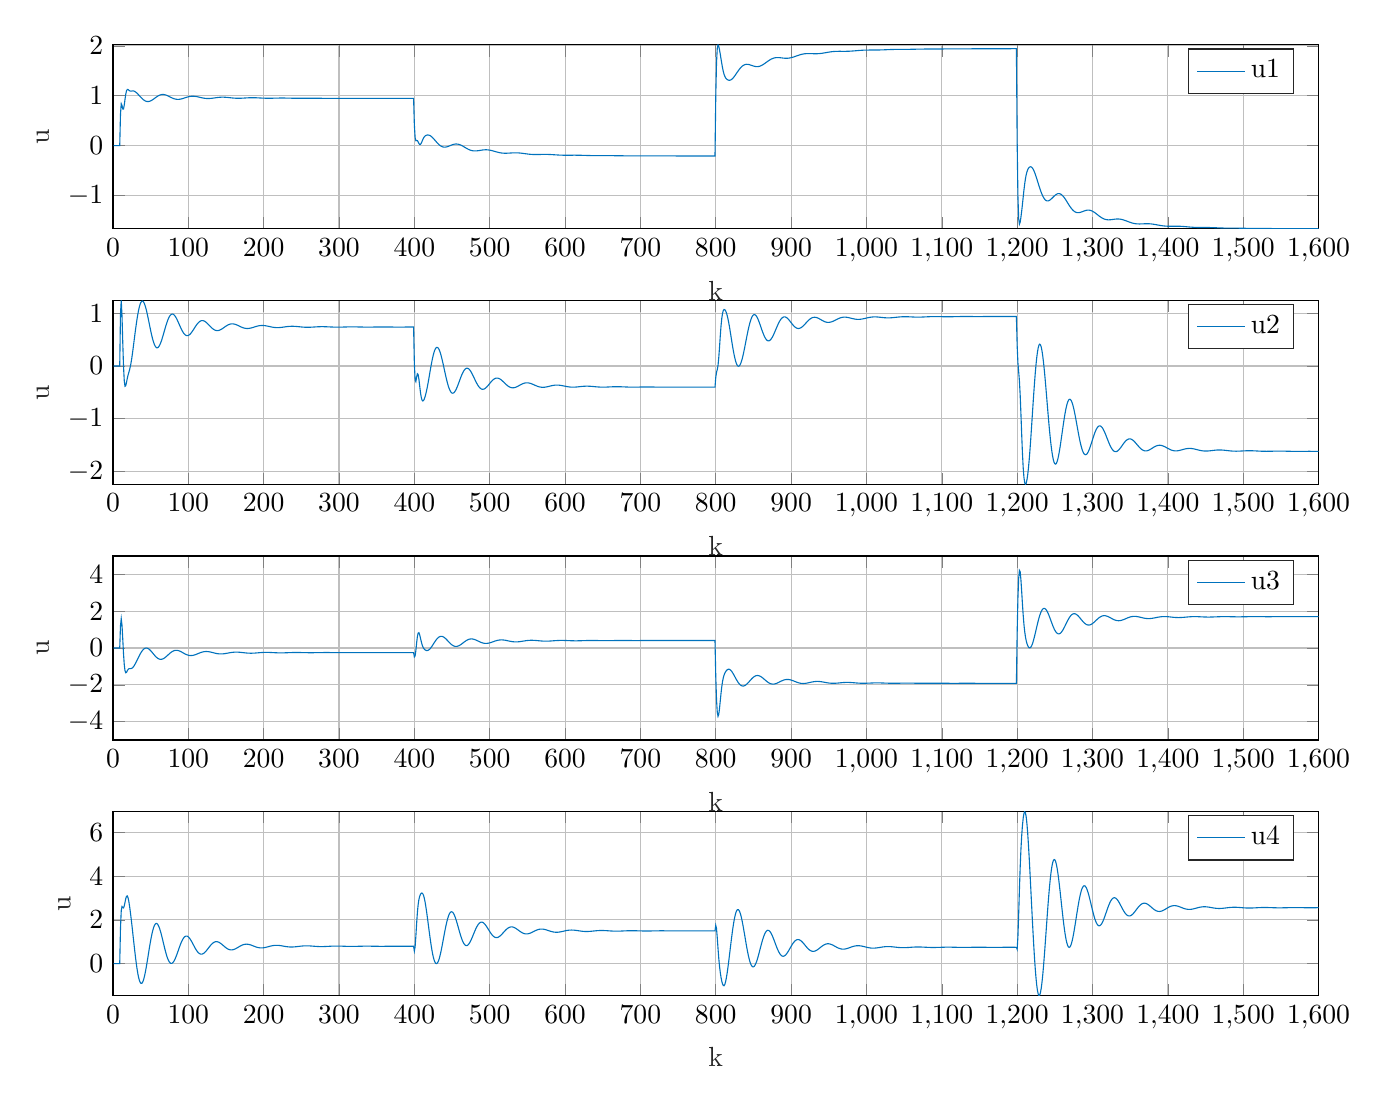
\begin{tikzpicture}

\begin{axis}[%
width=6.028in,
height=0.92in,
at={(1.011in,4.476in)},
scale only axis,
xmin=0,
xmax=1600,
xlabel style={font=\color{white!15!black}},
xlabel={k},
ymin=-1.664,
ymax=2.0206,
ylabel style={font=\color{white!15!black}},
ylabel={u},
axis background/.style={fill=white},
xmajorgrids,
ymajorgrids,
legend style={legend cell align=left, align=left, draw=white!15!black}
]
\addplot [color=mycolor1]
  table[row sep=crcr]{%
1	0\\
2	0\\
3	0\\
4	0\\
5	0\\
6	0\\
7	0\\
8	0\\
9	0\\
10	0.62841\\
11	0.84007\\
12	0.80706\\
13	0.73563\\
14	0.73494\\
15	0.81349\\
16	0.92809\\
17	1.0316\\
18	1.098\\
19	1.1248\\
20	1.1244\\
21	1.1122\\
22	1.1\\
23	1.0933\\
24	1.0923\\
25	1.0944\\
26	1.0965\\
27	1.0964\\
28	1.0928\\
29	1.0859\\
30	1.076\\
31	1.0637\\
32	1.0498\\
33	1.0347\\
34	1.0188\\
35	1.0024\\
36	0.98589\\
37	0.96963\\
38	0.95395\\
39	0.93921\\
40	0.92574\\
41	0.91381\\
42	0.90368\\
43	0.89552\\
44	0.88947\\
45	0.88558\\
46	0.88389\\
47	0.88434\\
48	0.88684\\
49	0.89126\\
50	0.89741\\
51	0.90508\\
52	0.91402\\
53	0.92397\\
54	0.93463\\
55	0.94571\\
56	0.95693\\
57	0.96801\\
58	0.97867\\
59	0.98866\\
60	0.99777\\
61	1.0058\\
62	1.0126\\
63	1.018\\
64	1.022\\
65	1.0245\\
66	1.0255\\
67	1.0251\\
68	1.0232\\
69	1.0201\\
70	1.0158\\
71	1.0104\\
72	1.0042\\
73	0.99737\\
74	0.99004\\
75	0.98242\\
76	0.97473\\
77	0.96714\\
78	0.95985\\
79	0.95301\\
80	0.94679\\
81	0.94129\\
82	0.93664\\
83	0.93291\\
84	0.93016\\
85	0.9284\\
86	0.92766\\
87	0.92789\\
88	0.92907\\
89	0.93111\\
90	0.93393\\
91	0.93743\\
92	0.9415\\
93	0.94601\\
94	0.95083\\
95	0.95582\\
96	0.96086\\
97	0.96581\\
98	0.97055\\
99	0.97497\\
100	0.97898\\
101	0.98248\\
102	0.98541\\
103	0.98771\\
104	0.98935\\
105	0.99031\\
106	0.99059\\
107	0.99022\\
108	0.98921\\
109	0.98761\\
110	0.9855\\
111	0.98293\\
112	0.97998\\
113	0.97675\\
114	0.97331\\
115	0.96976\\
116	0.96618\\
117	0.96267\\
118	0.9593\\
119	0.95616\\
120	0.9533\\
121	0.95078\\
122	0.94865\\
123	0.94695\\
124	0.94569\\
125	0.94489\\
126	0.94455\\
127	0.94465\\
128	0.94517\\
129	0.94609\\
130	0.94735\\
131	0.94891\\
132	0.95072\\
133	0.95273\\
134	0.95486\\
135	0.95707\\
136	0.95928\\
137	0.96145\\
138	0.96351\\
139	0.96542\\
140	0.96714\\
141	0.96862\\
142	0.96983\\
143	0.97076\\
144	0.97138\\
145	0.9717\\
146	0.97171\\
147	0.97142\\
148	0.97085\\
149	0.97001\\
150	0.96894\\
151	0.96768\\
152	0.96625\\
153	0.96469\\
154	0.96305\\
155	0.96136\\
156	0.95967\\
157	0.95802\\
158	0.95644\\
159	0.95496\\
160	0.95362\\
161	0.95244\\
162	0.95144\\
163	0.95064\\
164	0.95004\\
165	0.94965\\
166	0.94947\\
167	0.94949\\
168	0.9497\\
169	0.95008\\
170	0.95062\\
171	0.9513\\
172	0.95209\\
173	0.95295\\
174	0.95388\\
175	0.95483\\
176	0.95578\\
177	0.95671\\
178	0.95759\\
179	0.95839\\
180	0.95911\\
181	0.95971\\
182	0.9602\\
183	0.96055\\
184	0.96076\\
185	0.96084\\
186	0.96077\\
187	0.96057\\
188	0.96025\\
189	0.9598\\
190	0.95926\\
191	0.95862\\
192	0.95792\\
193	0.95716\\
194	0.95637\\
195	0.95555\\
196	0.95475\\
197	0.95396\\
198	0.95321\\
199	0.9525\\
200	0.95187\\
201	0.9513\\
202	0.95083\\
203	0.95044\\
204	0.95014\\
205	0.94995\\
206	0.94984\\
207	0.94983\\
208	0.9499\\
209	0.95006\\
210	0.95028\\
211	0.95056\\
212	0.9509\\
213	0.95126\\
214	0.95165\\
215	0.95206\\
216	0.95246\\
217	0.95285\\
218	0.95321\\
219	0.95354\\
220	0.95383\\
221	0.95407\\
222	0.95425\\
223	0.95437\\
224	0.95443\\
225	0.95443\\
226	0.95436\\
227	0.95424\\
228	0.95405\\
229	0.95382\\
230	0.95354\\
231	0.95322\\
232	0.95287\\
233	0.9525\\
234	0.95211\\
235	0.95172\\
236	0.95133\\
237	0.95095\\
238	0.95059\\
239	0.95025\\
240	0.94994\\
241	0.94967\\
242	0.94944\\
243	0.94925\\
244	0.9491\\
245	0.949\\
246	0.94894\\
247	0.94892\\
248	0.94894\\
249	0.949\\
250	0.94909\\
251	0.9492\\
252	0.94934\\
253	0.94949\\
254	0.94965\\
255	0.94982\\
256	0.94998\\
257	0.95014\\
258	0.95029\\
259	0.95042\\
260	0.95053\\
261	0.95062\\
262	0.95068\\
263	0.95072\\
264	0.95073\\
265	0.95071\\
266	0.95066\\
267	0.95058\\
268	0.95048\\
269	0.95036\\
270	0.95021\\
271	0.95005\\
272	0.94988\\
273	0.94969\\
274	0.9495\\
275	0.94931\\
276	0.94912\\
277	0.94894\\
278	0.94877\\
279	0.9486\\
280	0.94845\\
281	0.94832\\
282	0.94821\\
283	0.94811\\
284	0.94804\\
285	0.94799\\
286	0.94795\\
287	0.94794\\
288	0.94794\\
289	0.94796\\
290	0.94799\\
291	0.94803\\
292	0.94809\\
293	0.94815\\
294	0.94821\\
295	0.94828\\
296	0.94835\\
297	0.94841\\
298	0.94847\\
299	0.94852\\
300	0.94856\\
301	0.94859\\
302	0.94861\\
303	0.94861\\
304	0.94861\\
305	0.94859\\
306	0.94856\\
307	0.94851\\
308	0.94846\\
309	0.94839\\
310	0.94832\\
311	0.94824\\
312	0.94815\\
313	0.94806\\
314	0.94797\\
315	0.94787\\
316	0.94778\\
317	0.94769\\
318	0.94761\\
319	0.94753\\
320	0.94746\\
321	0.94739\\
322	0.94734\\
323	0.94729\\
324	0.94725\\
325	0.94722\\
326	0.9472\\
327	0.94719\\
328	0.94719\\
329	0.94719\\
330	0.9472\\
331	0.94722\\
332	0.94724\\
333	0.94727\\
334	0.94729\\
335	0.94732\\
336	0.94734\\
337	0.94737\\
338	0.94739\\
339	0.94741\\
340	0.94743\\
341	0.94744\\
342	0.94745\\
343	0.94745\\
344	0.94745\\
345	0.94744\\
346	0.94742\\
347	0.9474\\
348	0.94738\\
349	0.94735\\
350	0.94732\\
351	0.94729\\
352	0.94725\\
353	0.94721\\
354	0.94717\\
355	0.94713\\
356	0.9471\\
357	0.94706\\
358	0.94702\\
359	0.94699\\
360	0.94696\\
361	0.94693\\
362	0.94689\\
363	0.94686\\
364	0.94684\\
365	0.94681\\
366	0.9468\\
367	0.94678\\
368	0.94677\\
369	0.94676\\
370	0.94676\\
371	0.94675\\
372	0.94675\\
373	0.94675\\
374	0.94675\\
375	0.94675\\
376	0.94676\\
377	0.94676\\
378	0.94676\\
379	0.94677\\
380	0.94677\\
381	0.94677\\
382	0.94677\\
383	0.94677\\
384	0.94676\\
385	0.94676\\
386	0.94675\\
387	0.94674\\
388	0.94673\\
389	0.94672\\
390	0.94671\\
391	0.94669\\
392	0.94668\\
393	0.94666\\
394	0.94665\\
395	0.94663\\
396	0.94661\\
397	0.94659\\
398	0.94658\\
399	0.94656\\
400	0.42085\\
401	0.16475\\
402	0.09939\\
403	0.10325\\
404	0.10185\\
405	0.077564\\
406	0.044847\\
407	0.023474\\
408	0.023904\\
409	0.044989\\
410	0.07853\\
411	0.11505\\
412	0.1476\\
413	0.17294\\
414	0.1908\\
415	0.20247\\
416	0.20954\\
417	0.21321\\
418	0.21408\\
419	0.21232\\
420	0.20788\\
421	0.20074\\
422	0.19101\\
423	0.17892\\
424	0.16484\\
425	0.14919\\
426	0.13242\\
427	0.11496\\
428	0.097253\\
429	0.079676\\
430	0.062597\\
431	0.04635\\
432	0.031228\\
433	0.017484\\
434	0.0053263\\
435	-0.0050869\\
436	-0.013649\\
437	-0.020303\\
438	-0.025047\\
439	-0.027922\\
440	-0.029018\\
441	-0.028464\\
442	-0.026425\\
443	-0.023096\\
444	-0.018695\\
445	-0.013458\\
446	-0.0076325\\
447	-0.0014681\\
448	0.0047864\\
449	0.010891\\
450	0.01662\\
451	0.021766\\
452	0.026146\\
453	0.029605\\
454	0.032015\\
455	0.033283\\
456	0.033347\\
457	0.032179\\
458	0.029784\\
459	0.026197\\
460	0.021484\\
461	0.015736\\
462	0.0090662\\
463	0.0016091\\
464	-0.0064866\\
465	-0.015061\\
466	-0.023948\\
467	-0.032978\\
468	-0.041986\\
469	-0.05081\\
470	-0.0593\\
471	-0.067319\\
472	-0.074746\\
473	-0.081477\\
474	-0.087431\\
475	-0.092546\\
476	-0.096784\\
477	-0.10013\\
478	-0.10259\\
479	-0.10418\\
480	-0.10496\\
481	-0.10499\\
482	-0.10435\\
483	-0.10313\\
484	-0.10143\\
485	-0.099364\\
486	-0.097039\\
487	-0.094573\\
488	-0.092079\\
489	-0.089664\\
490	-0.087431\\
491	-0.085472\\
492	-0.083868\\
493	-0.082689\\
494	-0.08199\\
495	-0.08181\\
496	-0.082175\\
497	-0.083096\\
498	-0.084569\\
499	-0.086574\\
500	-0.08908\\
501	-0.092044\\
502	-0.095413\\
503	-0.099124\\
504	-0.10311\\
505	-0.10729\\
506	-0.1116\\
507	-0.11596\\
508	-0.12029\\
509	-0.12452\\
510	-0.12859\\
511	-0.13242\\
512	-0.13597\\
513	-0.1392\\
514	-0.14206\\
515	-0.14453\\
516	-0.1466\\
517	-0.14825\\
518	-0.1495\\
519	-0.15036\\
520	-0.15085\\
521	-0.15099\\
522	-0.15084\\
523	-0.15042\\
524	-0.14979\\
525	-0.149\\
526	-0.14809\\
527	-0.14713\\
528	-0.14616\\
529	-0.14523\\
530	-0.14438\\
531	-0.14367\\
532	-0.14311\\
533	-0.14276\\
534	-0.14262\\
535	-0.14272\\
536	-0.14306\\
537	-0.14366\\
538	-0.1445\\
539	-0.14558\\
540	-0.14688\\
541	-0.14839\\
542	-0.15007\\
543	-0.1519\\
544	-0.15385\\
545	-0.15588\\
546	-0.15796\\
547	-0.16005\\
548	-0.16212\\
549	-0.16415\\
550	-0.16608\\
551	-0.16791\\
552	-0.16961\\
553	-0.17115\\
554	-0.17252\\
555	-0.17371\\
556	-0.17471\\
557	-0.17552\\
558	-0.17615\\
559	-0.1766\\
560	-0.17688\\
561	-0.17701\\
562	-0.177\\
563	-0.17687\\
564	-0.17665\\
565	-0.17636\\
566	-0.17602\\
567	-0.17565\\
568	-0.17529\\
569	-0.17494\\
570	-0.17464\\
571	-0.17439\\
572	-0.17422\\
573	-0.17414\\
574	-0.17416\\
575	-0.17429\\
576	-0.17453\\
577	-0.17488\\
578	-0.17534\\
579	-0.17591\\
580	-0.17658\\
581	-0.17733\\
582	-0.17816\\
583	-0.17906\\
584	-0.18001\\
585	-0.18099\\
586	-0.18199\\
587	-0.183\\
588	-0.18399\\
589	-0.18495\\
590	-0.18587\\
591	-0.18674\\
592	-0.18755\\
593	-0.18828\\
594	-0.18894\\
595	-0.18951\\
596	-0.19\\
597	-0.1904\\
598	-0.19071\\
599	-0.19094\\
600	-0.1911\\
601	-0.19119\\
602	-0.19121\\
603	-0.19118\\
604	-0.19111\\
605	-0.19101\\
606	-0.19089\\
607	-0.19076\\
608	-0.19063\\
609	-0.19051\\
610	-0.1904\\
611	-0.19033\\
612	-0.19029\\
613	-0.19029\\
614	-0.19034\\
615	-0.19044\\
616	-0.19058\\
617	-0.19078\\
618	-0.19103\\
619	-0.19132\\
620	-0.19166\\
621	-0.19204\\
622	-0.19245\\
623	-0.19289\\
624	-0.19335\\
625	-0.19382\\
626	-0.1943\\
627	-0.19478\\
628	-0.19525\\
629	-0.19571\\
630	-0.19615\\
631	-0.19657\\
632	-0.19695\\
633	-0.1973\\
634	-0.19761\\
635	-0.19789\\
636	-0.19812\\
637	-0.19832\\
638	-0.19848\\
639	-0.19859\\
640	-0.19868\\
641	-0.19873\\
642	-0.19876\\
643	-0.19876\\
644	-0.19874\\
645	-0.19871\\
646	-0.19867\\
647	-0.19863\\
648	-0.19859\\
649	-0.19855\\
650	-0.19852\\
651	-0.1985\\
652	-0.1985\\
653	-0.19852\\
654	-0.19856\\
655	-0.19863\\
656	-0.19871\\
657	-0.19882\\
658	-0.19895\\
659	-0.1991\\
660	-0.19927\\
661	-0.19945\\
662	-0.19966\\
663	-0.19987\\
664	-0.20009\\
665	-0.20032\\
666	-0.20055\\
667	-0.20078\\
668	-0.20101\\
669	-0.20123\\
670	-0.20144\\
671	-0.20163\\
672	-0.20181\\
673	-0.20198\\
674	-0.20213\\
675	-0.20226\\
676	-0.20238\\
677	-0.20247\\
678	-0.20255\\
679	-0.20261\\
680	-0.20266\\
681	-0.20269\\
682	-0.20271\\
683	-0.20271\\
684	-0.20271\\
685	-0.20271\\
686	-0.2027\\
687	-0.20268\\
688	-0.20267\\
689	-0.20266\\
690	-0.20266\\
691	-0.20266\\
692	-0.20267\\
693	-0.20269\\
694	-0.20271\\
695	-0.20275\\
696	-0.2028\\
697	-0.20285\\
698	-0.20292\\
699	-0.203\\
700	-0.20308\\
701	-0.20318\\
702	-0.20327\\
703	-0.20338\\
704	-0.20349\\
705	-0.2036\\
706	-0.20371\\
707	-0.20382\\
708	-0.20392\\
709	-0.20403\\
710	-0.20413\\
711	-0.20422\\
712	-0.20431\\
713	-0.20439\\
714	-0.20446\\
715	-0.20452\\
716	-0.20458\\
717	-0.20463\\
718	-0.20466\\
719	-0.2047\\
720	-0.20472\\
721	-0.20474\\
722	-0.20475\\
723	-0.20476\\
724	-0.20476\\
725	-0.20476\\
726	-0.20476\\
727	-0.20476\\
728	-0.20476\\
729	-0.20476\\
730	-0.20476\\
731	-0.20477\\
732	-0.20478\\
733	-0.20479\\
734	-0.20481\\
735	-0.20483\\
736	-0.20486\\
737	-0.20489\\
738	-0.20492\\
739	-0.20496\\
740	-0.205\\
741	-0.20505\\
742	-0.2051\\
743	-0.20515\\
744	-0.2052\\
745	-0.20525\\
746	-0.2053\\
747	-0.20536\\
748	-0.20541\\
749	-0.20546\\
750	-0.2055\\
751	-0.20554\\
752	-0.20558\\
753	-0.20562\\
754	-0.20565\\
755	-0.20568\\
756	-0.20571\\
757	-0.20574\\
758	-0.20576\\
759	-0.20578\\
760	-0.2058\\
761	-0.20581\\
762	-0.20582\\
763	-0.20583\\
764	-0.20584\\
765	-0.20585\\
766	-0.20586\\
767	-0.20586\\
768	-0.20587\\
769	-0.20587\\
770	-0.20588\\
771	-0.20588\\
772	-0.20589\\
773	-0.2059\\
774	-0.2059\\
775	-0.20591\\
776	-0.20593\\
777	-0.20594\\
778	-0.20595\\
779	-0.20597\\
780	-0.20598\\
781	-0.206\\
782	-0.20602\\
783	-0.20603\\
784	-0.20605\\
785	-0.20607\\
786	-0.20609\\
787	-0.20611\\
788	-0.20613\\
789	-0.20615\\
790	-0.20617\\
791	-0.20619\\
792	-0.20621\\
793	-0.20623\\
794	-0.20624\\
795	-0.20626\\
796	-0.20627\\
797	-0.20629\\
798	-0.2063\\
799	-0.20631\\
800	0.97489\\
801	1.6588\\
802	1.9509\\
803	2.0206\\
804	1.9894\\
805	1.9185\\
806	1.8316\\
807	1.7381\\
808	1.6451\\
809	1.5596\\
810	1.4873\\
811	1.4307\\
812	1.3893\\
813	1.3602\\
814	1.3401\\
815	1.3263\\
816	1.3171\\
817	1.3117\\
818	1.3099\\
819	1.312\\
820	1.3178\\
821	1.3273\\
822	1.3402\\
823	1.3559\\
824	1.374\\
825	1.3939\\
826	1.4151\\
827	1.437\\
828	1.4592\\
829	1.4812\\
830	1.5027\\
831	1.5233\\
832	1.5426\\
833	1.5603\\
834	1.5762\\
835	1.5902\\
836	1.6021\\
837	1.6118\\
838	1.6194\\
839	1.6248\\
840	1.6283\\
841	1.6298\\
842	1.6296\\
843	1.6279\\
844	1.625\\
845	1.621\\
846	1.6163\\
847	1.6112\\
848	1.6059\\
849	1.6006\\
850	1.5957\\
851	1.5913\\
852	1.5878\\
853	1.5852\\
854	1.5836\\
855	1.5833\\
856	1.5843\\
857	1.5866\\
858	1.5903\\
859	1.5952\\
860	1.6014\\
861	1.6087\\
862	1.617\\
863	1.6262\\
864	1.6361\\
865	1.6466\\
866	1.6574\\
867	1.6684\\
868	1.6794\\
869	1.6903\\
870	1.7008\\
871	1.7108\\
872	1.7201\\
873	1.7287\\
874	1.7365\\
875	1.7433\\
876	1.7492\\
877	1.7541\\
878	1.758\\
879	1.7609\\
880	1.763\\
881	1.7641\\
882	1.7645\\
883	1.7643\\
884	1.7635\\
885	1.7622\\
886	1.7606\\
887	1.7588\\
888	1.757\\
889	1.7552\\
890	1.7535\\
891	1.7522\\
892	1.7511\\
893	1.7506\\
894	1.7505\\
895	1.751\\
896	1.752\\
897	1.7537\\
898	1.7559\\
899	1.7588\\
900	1.7621\\
901	1.766\\
902	1.7703\\
903	1.775\\
904	1.78\\
905	1.7852\\
906	1.7906\\
907	1.7961\\
908	1.8015\\
909	1.8068\\
910	1.8119\\
911	1.8168\\
912	1.8214\\
913	1.8257\\
914	1.8295\\
915	1.8329\\
916	1.8359\\
917	1.8384\\
918	1.8404\\
919	1.842\\
920	1.8432\\
921	1.844\\
922	1.8445\\
923	1.8446\\
924	1.8445\\
925	1.8442\\
926	1.8438\\
927	1.8432\\
928	1.8427\\
929	1.8422\\
930	1.8417\\
931	1.8414\\
932	1.8412\\
933	1.8413\\
934	1.8415\\
935	1.842\\
936	1.8428\\
937	1.8439\\
938	1.8452\\
939	1.8467\\
940	1.8485\\
941	1.8505\\
942	1.8528\\
943	1.8552\\
944	1.8577\\
945	1.8603\\
946	1.8629\\
947	1.8656\\
948	1.8683\\
949	1.8709\\
950	1.8734\\
951	1.8758\\
952	1.878\\
953	1.8801\\
954	1.882\\
955	1.8837\\
956	1.8852\\
957	1.8865\\
958	1.8875\\
959	1.8884\\
960	1.8891\\
961	1.8896\\
962	1.8899\\
963	1.8901\\
964	1.8902\\
965	1.8902\\
966	1.8901\\
967	1.89\\
968	1.8899\\
969	1.8898\\
970	1.8898\\
971	1.8898\\
972	1.8898\\
973	1.89\\
974	1.8903\\
975	1.8906\\
976	1.8911\\
977	1.8917\\
978	1.8925\\
979	1.8933\\
980	1.8943\\
981	1.8953\\
982	1.8964\\
983	1.8976\\
984	1.8989\\
985	1.9002\\
986	1.9015\\
987	1.9028\\
988	1.9041\\
989	1.9054\\
990	1.9066\\
991	1.9078\\
992	1.9089\\
993	1.9099\\
994	1.9109\\
995	1.9117\\
996	1.9125\\
997	1.9131\\
998	1.9137\\
999	1.9141\\
1000	1.9145\\
1001	1.9148\\
1002	1.915\\
1003	1.9151\\
1004	1.9153\\
1005	1.9153\\
1006	1.9154\\
1007	1.9154\\
1008	1.9154\\
1009	1.9154\\
1010	1.9155\\
1011	1.9155\\
1012	1.9156\\
1013	1.9158\\
1014	1.916\\
1015	1.9162\\
1016	1.9165\\
1017	1.9168\\
1018	1.9172\\
1019	1.9177\\
1020	1.9182\\
1021	1.9187\\
1022	1.9193\\
1023	1.9199\\
1024	1.9205\\
1025	1.9211\\
1026	1.9218\\
1027	1.9224\\
1028	1.9231\\
1029	1.9237\\
1030	1.9243\\
1031	1.9249\\
1032	1.9254\\
1033	1.9259\\
1034	1.9264\\
1035	1.9268\\
1036	1.9272\\
1037	1.9275\\
1038	1.9278\\
1039	1.928\\
1040	1.9282\\
1041	1.9284\\
1042	1.9285\\
1043	1.9286\\
1044	1.9287\\
1045	1.9288\\
1046	1.9288\\
1047	1.9289\\
1048	1.9289\\
1049	1.9289\\
1050	1.929\\
1051	1.9291\\
1052	1.9291\\
1053	1.9292\\
1054	1.9294\\
1055	1.9295\\
1056	1.9297\\
1057	1.9299\\
1058	1.9301\\
1059	1.9303\\
1060	1.9306\\
1061	1.9308\\
1062	1.9311\\
1063	1.9314\\
1064	1.9317\\
1065	1.932\\
1066	1.9324\\
1067	1.9327\\
1068	1.933\\
1069	1.9333\\
1070	1.9336\\
1071	1.9339\\
1072	1.9341\\
1073	1.9344\\
1074	1.9346\\
1075	1.9348\\
1076	1.935\\
1077	1.9352\\
1078	1.9353\\
1079	1.9354\\
1080	1.9356\\
1081	1.9356\\
1082	1.9357\\
1083	1.9358\\
1084	1.9358\\
1085	1.9359\\
1086	1.9359\\
1087	1.9359\\
1088	1.936\\
1089	1.936\\
1090	1.9361\\
1091	1.9361\\
1092	1.9362\\
1093	1.9362\\
1094	1.9363\\
1095	1.9364\\
1096	1.9365\\
1097	1.9366\\
1098	1.9367\\
1099	1.9368\\
1100	1.9369\\
1101	1.9371\\
1102	1.9372\\
1103	1.9374\\
1104	1.9375\\
1105	1.9377\\
1106	1.9378\\
1107	1.938\\
1108	1.9381\\
1109	1.9383\\
1110	1.9384\\
1111	1.9386\\
1112	1.9387\\
1113	1.9388\\
1114	1.9389\\
1115	1.939\\
1116	1.9391\\
1117	1.9392\\
1118	1.9393\\
1119	1.9393\\
1120	1.9394\\
1121	1.9394\\
1122	1.9395\\
1123	1.9395\\
1124	1.9396\\
1125	1.9396\\
1126	1.9396\\
1127	1.9396\\
1128	1.9397\\
1129	1.9397\\
1130	1.9397\\
1131	1.9397\\
1132	1.9398\\
1133	1.9398\\
1134	1.9399\\
1135	1.9399\\
1136	1.94\\
1137	1.94\\
1138	1.9401\\
1139	1.9401\\
1140	1.9402\\
1141	1.9403\\
1142	1.9403\\
1143	1.9404\\
1144	1.9405\\
1145	1.9406\\
1146	1.9407\\
1147	1.9407\\
1148	1.9408\\
1149	1.9409\\
1150	1.941\\
1151	1.941\\
1152	1.9411\\
1153	1.9411\\
1154	1.9412\\
1155	1.9412\\
1156	1.9413\\
1157	1.9413\\
1158	1.9414\\
1159	1.9414\\
1160	1.9414\\
1161	1.9415\\
1162	1.9415\\
1163	1.9415\\
1164	1.9415\\
1165	1.9416\\
1166	1.9416\\
1167	1.9416\\
1168	1.9416\\
1169	1.9416\\
1170	1.9417\\
1171	1.9417\\
1172	1.9417\\
1173	1.9417\\
1174	1.9417\\
1175	1.9418\\
1176	1.9418\\
1177	1.9418\\
1178	1.9418\\
1179	1.9419\\
1180	1.9419\\
1181	1.9419\\
1182	1.9419\\
1183	1.942\\
1184	1.942\\
1185	1.942\\
1186	1.9421\\
1187	1.9421\\
1188	1.9421\\
1189	1.9422\\
1190	1.9422\\
1191	1.9422\\
1192	1.9423\\
1193	1.9423\\
1194	1.9423\\
1195	1.9423\\
1196	1.9424\\
1197	1.9424\\
1198	1.9424\\
1199	1.9424\\
1200	0.077903\\
1201	-1.0026\\
1202	-1.4608\\
1203	-1.5711\\
1204	-1.5302\\
1205	-1.4332\\
1206	-1.3119\\
1207	-1.1752\\
1208	-1.0311\\
1209	-0.89076\\
1210	-0.76529\\
1211	-0.66181\\
1212	-0.58203\\
1213	-0.52347\\
1214	-0.48182\\
1215	-0.45296\\
1216	-0.43406\\
1217	-0.42373\\
1218	-0.42158\\
1219	-0.42764\\
1220	-0.44187\\
1221	-0.46393\\
1222	-0.49312\\
1223	-0.52848\\
1224	-0.56889\\
1225	-0.61314\\
1226	-0.66007\\
1227	-0.70852\\
1228	-0.75742\\
1229	-0.80575\\
1230	-0.85256\\
1231	-0.897\\
1232	-0.93832\\
1233	-0.97586\\
1234	-1.0091\\
1235	-1.0377\\
1236	-1.0613\\
1237	-1.0798\\
1238	-1.0933\\
1239	-1.1019\\
1240	-1.1057\\
1241	-1.1053\\
1242	-1.1009\\
1243	-1.0932\\
1244	-1.0827\\
1245	-1.0701\\
1246	-1.0559\\
1247	-1.0408\\
1248	-1.0256\\
1249	-1.0107\\
1250	-0.99689\\
1251	-0.9846\\
1252	-0.97431\\
1253	-0.96645\\
1254	-0.96133\\
1255	-0.95919\\
1256	-0.96019\\
1257	-0.96439\\
1258	-0.97178\\
1259	-0.98226\\
1260	-0.99566\\
1261	-1.0117\\
1262	-1.0302\\
1263	-1.0506\\
1264	-1.0727\\
1265	-1.096\\
1266	-1.1201\\
1267	-1.1445\\
1268	-1.1688\\
1269	-1.1926\\
1270	-1.2155\\
1271	-1.2371\\
1272	-1.2572\\
1273	-1.2754\\
1274	-1.2915\\
1275	-1.3055\\
1276	-1.3171\\
1277	-1.3265\\
1278	-1.3335\\
1279	-1.3382\\
1280	-1.3408\\
1281	-1.3415\\
1282	-1.3404\\
1283	-1.3378\\
1284	-1.334\\
1285	-1.3292\\
1286	-1.3238\\
1287	-1.318\\
1288	-1.3122\\
1289	-1.3066\\
1290	-1.3014\\
1291	-1.297\\
1292	-1.2935\\
1293	-1.2911\\
1294	-1.29\\
1295	-1.2903\\
1296	-1.2919\\
1297	-1.295\\
1298	-1.2995\\
1299	-1.3054\\
1300	-1.3126\\
1301	-1.321\\
1302	-1.3304\\
1303	-1.3407\\
1304	-1.3517\\
1305	-1.3632\\
1306	-1.375\\
1307	-1.3869\\
1308	-1.3987\\
1309	-1.4103\\
1310	-1.4214\\
1311	-1.4318\\
1312	-1.4415\\
1313	-1.4504\\
1314	-1.4583\\
1315	-1.4652\\
1316	-1.471\\
1317	-1.4757\\
1318	-1.4794\\
1319	-1.482\\
1320	-1.4837\\
1321	-1.4844\\
1322	-1.4844\\
1323	-1.4838\\
1324	-1.4825\\
1325	-1.4809\\
1326	-1.4789\\
1327	-1.4768\\
1328	-1.4747\\
1329	-1.4727\\
1330	-1.471\\
1331	-1.4695\\
1332	-1.4685\\
1333	-1.468\\
1334	-1.4681\\
1335	-1.4688\\
1336	-1.4701\\
1337	-1.4721\\
1338	-1.4747\\
1339	-1.4779\\
1340	-1.4817\\
1341	-1.4861\\
1342	-1.4908\\
1343	-1.496\\
1344	-1.5014\\
1345	-1.5071\\
1346	-1.5129\\
1347	-1.5187\\
1348	-1.5244\\
1349	-1.53\\
1350	-1.5354\\
1351	-1.5405\\
1352	-1.5452\\
1353	-1.5495\\
1354	-1.5533\\
1355	-1.5567\\
1356	-1.5596\\
1357	-1.562\\
1358	-1.5639\\
1359	-1.5653\\
1360	-1.5663\\
1361	-1.5669\\
1362	-1.5672\\
1363	-1.5671\\
1364	-1.5668\\
1365	-1.5663\\
1366	-1.5657\\
1367	-1.565\\
1368	-1.5643\\
1369	-1.5636\\
1370	-1.5631\\
1371	-1.5627\\
1372	-1.5626\\
1373	-1.5626\\
1374	-1.5629\\
1375	-1.5635\\
1376	-1.5644\\
1377	-1.5656\\
1378	-1.567\\
1379	-1.5688\\
1380	-1.5707\\
1381	-1.573\\
1382	-1.5754\\
1383	-1.5779\\
1384	-1.5806\\
1385	-1.5834\\
1386	-1.5862\\
1387	-1.5891\\
1388	-1.5919\\
1389	-1.5946\\
1390	-1.5972\\
1391	-1.5996\\
1392	-1.6019\\
1393	-1.604\\
1394	-1.6059\\
1395	-1.6076\\
1396	-1.609\\
1397	-1.6102\\
1398	-1.6112\\
1399	-1.612\\
1400	-1.6125\\
1401	-1.6129\\
1402	-1.6131\\
1403	-1.6132\\
1404	-1.6132\\
1405	-1.6131\\
1406	-1.613\\
1407	-1.6128\\
1408	-1.6126\\
1409	-1.6124\\
1410	-1.6123\\
1411	-1.6123\\
1412	-1.6123\\
1413	-1.6125\\
1414	-1.6128\\
1415	-1.6132\\
1416	-1.6137\\
1417	-1.6144\\
1418	-1.6152\\
1419	-1.6161\\
1420	-1.6171\\
1421	-1.6182\\
1422	-1.6194\\
1423	-1.6207\\
1424	-1.622\\
1425	-1.6234\\
1426	-1.6248\\
1427	-1.6262\\
1428	-1.6275\\
1429	-1.6288\\
1430	-1.6301\\
1431	-1.6313\\
1432	-1.6324\\
1433	-1.6334\\
1434	-1.6343\\
1435	-1.6352\\
1436	-1.6359\\
1437	-1.6365\\
1438	-1.637\\
1439	-1.6374\\
1440	-1.6377\\
1441	-1.6379\\
1442	-1.6381\\
1443	-1.6382\\
1444	-1.6383\\
1445	-1.6383\\
1446	-1.6383\\
1447	-1.6382\\
1448	-1.6382\\
1449	-1.6382\\
1450	-1.6382\\
1451	-1.6383\\
1452	-1.6384\\
1453	-1.6385\\
1454	-1.6387\\
1455	-1.6389\\
1456	-1.6393\\
1457	-1.6396\\
1458	-1.64\\
1459	-1.6405\\
1460	-1.641\\
1461	-1.6416\\
1462	-1.6422\\
1463	-1.6428\\
1464	-1.6435\\
1465	-1.6442\\
1466	-1.6448\\
1467	-1.6455\\
1468	-1.6462\\
1469	-1.6468\\
1470	-1.6474\\
1471	-1.648\\
1472	-1.6485\\
1473	-1.649\\
1474	-1.6495\\
1475	-1.6499\\
1476	-1.6502\\
1477	-1.6505\\
1478	-1.6508\\
1479	-1.651\\
1480	-1.6512\\
1481	-1.6513\\
1482	-1.6514\\
1483	-1.6515\\
1484	-1.6516\\
1485	-1.6516\\
1486	-1.6516\\
1487	-1.6516\\
1488	-1.6517\\
1489	-1.6517\\
1490	-1.6517\\
1491	-1.6518\\
1492	-1.6519\\
1493	-1.652\\
1494	-1.6521\\
1495	-1.6522\\
1496	-1.6524\\
1497	-1.6526\\
1498	-1.6528\\
1499	-1.653\\
1500	-1.6533\\
1501	-1.6536\\
1502	-1.6539\\
1503	-1.6542\\
1504	-1.6545\\
1505	-1.6549\\
1506	-1.6552\\
1507	-1.6555\\
1508	-1.6558\\
1509	-1.6561\\
1510	-1.6564\\
1511	-1.6567\\
1512	-1.657\\
1513	-1.6572\\
1514	-1.6574\\
1515	-1.6576\\
1516	-1.6578\\
1517	-1.658\\
1518	-1.6581\\
1519	-1.6582\\
1520	-1.6583\\
1521	-1.6584\\
1522	-1.6584\\
1523	-1.6585\\
1524	-1.6585\\
1525	-1.6586\\
1526	-1.6586\\
1527	-1.6586\\
1528	-1.6587\\
1529	-1.6587\\
1530	-1.6587\\
1531	-1.6588\\
1532	-1.6588\\
1533	-1.6589\\
1534	-1.6589\\
1535	-1.659\\
1536	-1.6591\\
1537	-1.6592\\
1538	-1.6593\\
1539	-1.6595\\
1540	-1.6596\\
1541	-1.6597\\
1542	-1.6599\\
1543	-1.6601\\
1544	-1.6602\\
1545	-1.6604\\
1546	-1.6605\\
1547	-1.6607\\
1548	-1.6608\\
1549	-1.661\\
1550	-1.6611\\
1551	-1.6613\\
1552	-1.6614\\
1553	-1.6615\\
1554	-1.6616\\
1555	-1.6617\\
1556	-1.6618\\
1557	-1.6619\\
1558	-1.662\\
1559	-1.662\\
1560	-1.6621\\
1561	-1.6621\\
1562	-1.6622\\
1563	-1.6622\\
1564	-1.6623\\
1565	-1.6623\\
1566	-1.6623\\
1567	-1.6624\\
1568	-1.6624\\
1569	-1.6624\\
1570	-1.6625\\
1571	-1.6625\\
1572	-1.6625\\
1573	-1.6625\\
1574	-1.6626\\
1575	-1.6626\\
1576	-1.6627\\
1577	-1.6627\\
1578	-1.6628\\
1579	-1.6628\\
1580	-1.6629\\
1581	-1.6629\\
1582	-1.663\\
1583	-1.663\\
1584	-1.6631\\
1585	-1.6632\\
1586	-1.6632\\
1587	-1.6633\\
1588	-1.6633\\
1589	-1.6634\\
1590	-1.6635\\
1591	-1.6635\\
1592	-1.6636\\
1593	-1.6636\\
1594	-1.6637\\
1595	-1.6638\\
1596	-1.6638\\
1597	-1.6638\\
1598	-1.6639\\
1599	-1.6639\\
1600	-1.664\\
};
\addlegendentry{u1}

\end{axis}

\begin{axis}[%
width=6.028in,
height=0.92in,
at={(1.011in,3.198in)},
scale only axis,
xmin=0,
xmax=1600,
xlabel style={font=\color{white!15!black}},
xlabel={k},
ymin=-2.2448,
ymax=1.2438,
ylabel style={font=\color{white!15!black}},
ylabel={u},
axis background/.style={fill=white},
xmajorgrids,
ymajorgrids,
legend style={legend cell align=left, align=left, draw=white!15!black}
]
\addplot [color=mycolor1]
  table[row sep=crcr]{%
1	0\\
2	0\\
3	0\\
4	0\\
5	0\\
6	0\\
7	0\\
8	0\\
9	0\\
10	0.98601\\
11	1.2438\\
12	0.95691\\
13	0.45557\\
14	0.003124\\
15	-0.27794\\
16	-0.38411\\
17	-0.37246\\
18	-0.30836\\
19	-0.23672\\
20	-0.17594\\
21	-0.12502\\
22	-0.074443\\
23	-0.014715\\
24	0.05947\\
25	0.14866\\
26	0.25005\\
27	0.35935\\
28	0.47216\\
29	0.58472\\
30	0.69399\\
31	0.79757\\
32	0.89343\\
33	0.97982\\
34	1.0552\\
35	1.1183\\
36	1.168\\
37	1.2036\\
38	1.225\\
39	1.2321\\
40	1.2253\\
41	1.2055\\
42	1.1736\\
43	1.131\\
44	1.0792\\
45	1.0199\\
46	0.95483\\
47	0.88593\\
48	0.81507\\
49	0.74413\\
50	0.6749\\
51	0.60907\\
52	0.54818\\
53	0.49356\\
54	0.44638\\
55	0.40754\\
56	0.37771\\
57	0.35733\\
58	0.34655\\
59	0.34531\\
60	0.35331\\
61	0.37\\
62	0.39468\\
63	0.42646\\
64	0.46429\\
65	0.50705\\
66	0.5535\\
67	0.60238\\
68	0.65241\\
69	0.70234\\
70	0.75096\\
71	0.79713\\
72	0.83984\\
73	0.87818\\
74	0.91139\\
75	0.93887\\
76	0.96018\\
77	0.97505\\
78	0.98338\\
79	0.98524\\
80	0.98084\\
81	0.97055\\
82	0.95487\\
83	0.93441\\
84	0.90987\\
85	0.88203\\
86	0.85173\\
87	0.81981\\
88	0.78714\\
89	0.75456\\
90	0.7229\\
91	0.69291\\
92	0.66526\\
93	0.64058\\
94	0.61935\\
95	0.60199\\
96	0.58877\\
97	0.57987\\
98	0.57536\\
99	0.57518\\
100	0.57916\\
101	0.58707\\
102	0.59856\\
103	0.61321\\
104	0.63055\\
105	0.65004\\
106	0.67113\\
107	0.69323\\
108	0.71577\\
109	0.73818\\
110	0.75991\\
111	0.78045\\
112	0.79935\\
113	0.81621\\
114	0.83069\\
115	0.84253\\
116	0.85154\\
117	0.85762\\
118	0.86072\\
119	0.86089\\
120	0.85824\\
121	0.85295\\
122	0.84525\\
123	0.83543\\
124	0.82381\\
125	0.81076\\
126	0.79665\\
127	0.78187\\
128	0.76682\\
129	0.75187\\
130	0.7374\\
131	0.72375\\
132	0.71122\\
133	0.70007\\
134	0.69054\\
135	0.68279\\
136	0.67695\\
137	0.67308\\
138	0.67121\\
139	0.6713\\
140	0.67329\\
141	0.67703\\
142	0.68238\\
143	0.68913\\
144	0.69708\\
145	0.70596\\
146	0.71553\\
147	0.72552\\
148	0.73567\\
149	0.74573\\
150	0.75543\\
151	0.76457\\
152	0.77292\\
153	0.78032\\
154	0.78662\\
155	0.79171\\
156	0.7955\\
157	0.79795\\
158	0.79905\\
159	0.79882\\
160	0.79733\\
161	0.79464\\
162	0.79089\\
163	0.78619\\
164	0.7807\\
165	0.77459\\
166	0.76803\\
167	0.76119\\
168	0.75426\\
169	0.74741\\
170	0.7408\\
171	0.73459\\
172	0.72891\\
173	0.72388\\
174	0.7196\\
175	0.71614\\
176	0.71356\\
177	0.71188\\
178	0.71111\\
179	0.71123\\
180	0.71221\\
181	0.71397\\
182	0.71646\\
183	0.71957\\
184	0.7232\\
185	0.72724\\
186	0.73158\\
187	0.73609\\
188	0.74066\\
189	0.74516\\
190	0.74949\\
191	0.75355\\
192	0.75723\\
193	0.76047\\
194	0.76321\\
195	0.76538\\
196	0.76696\\
197	0.76793\\
198	0.76828\\
199	0.76804\\
200	0.76723\\
201	0.76588\\
202	0.76406\\
203	0.76181\\
204	0.75922\\
205	0.75636\\
206	0.75331\\
207	0.75015\\
208	0.74696\\
209	0.74382\\
210	0.7408\\
211	0.73797\\
212	0.7354\\
213	0.73313\\
214	0.7312\\
215	0.72966\\
216	0.72852\\
217	0.72779\\
218	0.72747\\
219	0.72756\\
220	0.72804\\
221	0.72887\\
222	0.73002\\
223	0.73144\\
224	0.7331\\
225	0.73494\\
226	0.7369\\
227	0.73894\\
228	0.74099\\
229	0.743\\
230	0.74493\\
231	0.74672\\
232	0.74834\\
233	0.74976\\
234	0.75094\\
235	0.75186\\
236	0.75251\\
237	0.75288\\
238	0.75298\\
239	0.7528\\
240	0.75237\\
241	0.7517\\
242	0.75082\\
243	0.74975\\
244	0.74853\\
245	0.74719\\
246	0.74577\\
247	0.74431\\
248	0.74284\\
249	0.7414\\
250	0.74002\\
251	0.73873\\
252	0.73756\\
253	0.73654\\
254	0.73567\\
255	0.73498\\
256	0.73448\\
257	0.73416\\
258	0.73403\\
259	0.73408\\
260	0.73431\\
261	0.7347\\
262	0.73523\\
263	0.73588\\
264	0.73664\\
265	0.73747\\
266	0.73836\\
267	0.73927\\
268	0.74019\\
269	0.74109\\
270	0.74194\\
271	0.74274\\
272	0.74345\\
273	0.74406\\
274	0.74457\\
275	0.74496\\
276	0.74522\\
277	0.74536\\
278	0.74537\\
279	0.74526\\
280	0.74504\\
281	0.7447\\
282	0.74428\\
283	0.74377\\
284	0.74319\\
285	0.74257\\
286	0.74191\\
287	0.74123\\
288	0.74055\\
289	0.73989\\
290	0.73926\\
291	0.73867\\
292	0.73814\\
293	0.73768\\
294	0.73729\\
295	0.73698\\
296	0.73676\\
297	0.73662\\
298	0.73657\\
299	0.7366\\
300	0.7367\\
301	0.73688\\
302	0.73713\\
303	0.73743\\
304	0.73777\\
305	0.73815\\
306	0.73854\\
307	0.73896\\
308	0.73937\\
309	0.73977\\
310	0.74014\\
311	0.74049\\
312	0.7408\\
313	0.74107\\
314	0.74129\\
315	0.74145\\
316	0.74155\\
317	0.7416\\
318	0.74159\\
319	0.74153\\
320	0.74141\\
321	0.74125\\
322	0.74104\\
323	0.7408\\
324	0.74053\\
325	0.74024\\
326	0.73993\\
327	0.73962\\
328	0.7393\\
329	0.739\\
330	0.73871\\
331	0.73844\\
332	0.7382\\
333	0.73799\\
334	0.73781\\
335	0.73767\\
336	0.73757\\
337	0.73751\\
338	0.73748\\
339	0.73749\\
340	0.73754\\
341	0.73762\\
342	0.73773\\
343	0.73786\\
344	0.73801\\
345	0.73817\\
346	0.73835\\
347	0.73853\\
348	0.73871\\
349	0.73889\\
350	0.73905\\
351	0.73921\\
352	0.73934\\
353	0.73946\\
354	0.73955\\
355	0.73963\\
356	0.73967\\
357	0.73969\\
358	0.73969\\
359	0.73966\\
360	0.73961\\
361	0.73954\\
362	0.73945\\
363	0.73935\\
364	0.73924\\
365	0.73912\\
366	0.73899\\
367	0.73886\\
368	0.73873\\
369	0.73861\\
370	0.73848\\
371	0.73837\\
372	0.73827\\
373	0.73818\\
374	0.7381\\
375	0.73804\\
376	0.73799\\
377	0.73796\\
378	0.73795\\
379	0.73794\\
380	0.73795\\
381	0.73797\\
382	0.73801\\
383	0.73805\\
384	0.7381\\
385	0.73815\\
386	0.73821\\
387	0.73827\\
388	0.73833\\
389	0.73839\\
390	0.73845\\
391	0.7385\\
392	0.73854\\
393	0.73858\\
394	0.73861\\
395	0.73864\\
396	0.73865\\
397	0.73866\\
398	0.73866\\
399	0.73865\\
400	0.05362\\
401	-0.26477\\
402	-0.2972\\
403	-0.21276\\
404	-0.14701\\
405	-0.15938\\
406	-0.2451\\
407	-0.36791\\
408	-0.48907\\
409	-0.58301\\
410	-0.64019\\
411	-0.6626\\
412	-0.65748\\
413	-0.63239\\
414	-0.59287\\
415	-0.54216\\
416	-0.482\\
417	-0.41357\\
418	-0.33826\\
419	-0.25789\\
420	-0.17469\\
421	-0.091115\\
422	-0.0096186\\
423	0.067514\\
424	0.13826\\
425	0.20088\\
426	0.25398\\
427	0.29645\\
428	0.3275\\
429	0.34667\\
430	0.3538\\
431	0.34904\\
432	0.33282\\
433	0.30586\\
434	0.26911\\
435	0.22375\\
436	0.17111\\
437	0.11267\\
438	0.049976\\
439	-0.015351\\
440	-0.081701\\
441	-0.1475\\
442	-0.21123\\
443	-0.2715\\
444	-0.32706\\
445	-0.37679\\
446	-0.4198\\
447	-0.45536\\
448	-0.48298\\
449	-0.50237\\
450	-0.51344\\
451	-0.51635\\
452	-0.5114\\
453	-0.49912\\
454	-0.48016\\
455	-0.45533\\
456	-0.42556\\
457	-0.39184\\
458	-0.35524\\
459	-0.31685\\
460	-0.27775\\
461	-0.23902\\
462	-0.20166\\
463	-0.16661\\
464	-0.13472\\
465	-0.10673\\
466	-0.083228\\
467	-0.064696\\
468	-0.051461\\
469	-0.043706\\
470	-0.041471\\
471	-0.044659\\
472	-0.053038\\
473	-0.066258\\
474	-0.083862\\
475	-0.1053\\
476	-0.12995\\
477	-0.15713\\
478	-0.18613\\
479	-0.2162\\
480	-0.24663\\
481	-0.27668\\
482	-0.30569\\
483	-0.33302\\
484	-0.35811\\
485	-0.38048\\
486	-0.39972\\
487	-0.41554\\
488	-0.4277\\
489	-0.43611\\
490	-0.44073\\
491	-0.44165\\
492	-0.43903\\
493	-0.43311\\
494	-0.42421\\
495	-0.41271\\
496	-0.39902\\
497	-0.38361\\
498	-0.36696\\
499	-0.34958\\
500	-0.33196\\
501	-0.31458\\
502	-0.29789\\
503	-0.28232\\
504	-0.26824\\
505	-0.25598\\
506	-0.2458\\
507	-0.23791\\
508	-0.23245\\
509	-0.22948\\
510	-0.22902\\
511	-0.23102\\
512	-0.23535\\
513	-0.24185\\
514	-0.2503\\
515	-0.26045\\
516	-0.27202\\
517	-0.28468\\
518	-0.29811\\
519	-0.31198\\
520	-0.32594\\
521	-0.33969\\
522	-0.35291\\
523	-0.36532\\
524	-0.37667\\
525	-0.38675\\
526	-0.39538\\
527	-0.40243\\
528	-0.4078\\
529	-0.41146\\
530	-0.41339\\
531	-0.41365\\
532	-0.41232\\
533	-0.4095\\
534	-0.40535\\
535	-0.40004\\
536	-0.39377\\
537	-0.38675\\
538	-0.37921\\
539	-0.37136\\
540	-0.36344\\
541	-0.35566\\
542	-0.34823\\
543	-0.34133\\
544	-0.33514\\
545	-0.3298\\
546	-0.32541\\
547	-0.32208\\
548	-0.31986\\
549	-0.31878\\
550	-0.31884\\
551	-0.32\\
552	-0.32221\\
553	-0.3254\\
554	-0.32946\\
555	-0.33426\\
556	-0.33969\\
557	-0.34559\\
558	-0.35181\\
559	-0.35821\\
560	-0.36462\\
561	-0.37091\\
562	-0.37694\\
563	-0.38258\\
564	-0.38772\\
565	-0.39227\\
566	-0.39614\\
567	-0.39928\\
568	-0.40166\\
569	-0.40325\\
570	-0.40407\\
571	-0.40412\\
572	-0.40345\\
573	-0.40212\\
574	-0.40019\\
575	-0.39775\\
576	-0.39489\\
577	-0.3917\\
578	-0.38829\\
579	-0.38475\\
580	-0.3812\\
581	-0.37773\\
582	-0.37442\\
583	-0.37138\\
584	-0.36867\\
585	-0.36635\\
586	-0.36447\\
587	-0.36308\\
588	-0.36219\\
589	-0.36183\\
590	-0.36197\\
591	-0.36262\\
592	-0.36374\\
593	-0.3653\\
594	-0.36724\\
595	-0.36951\\
596	-0.37206\\
597	-0.37481\\
598	-0.37769\\
599	-0.38064\\
600	-0.38359\\
601	-0.38647\\
602	-0.38922\\
603	-0.39178\\
604	-0.39411\\
605	-0.39616\\
606	-0.3979\\
607	-0.39931\\
608	-0.40036\\
609	-0.40106\\
610	-0.4014\\
611	-0.40139\\
612	-0.40107\\
613	-0.40044\\
614	-0.39955\\
615	-0.39843\\
616	-0.39712\\
617	-0.39568\\
618	-0.39414\\
619	-0.39255\\
620	-0.39096\\
621	-0.38941\\
622	-0.38795\\
623	-0.38661\\
624	-0.38542\\
625	-0.38442\\
626	-0.38362\\
627	-0.38305\\
628	-0.3827\\
629	-0.38259\\
630	-0.38272\\
631	-0.38307\\
632	-0.38363\\
633	-0.38439\\
634	-0.38532\\
635	-0.38639\\
636	-0.38758\\
637	-0.38886\\
638	-0.3902\\
639	-0.39156\\
640	-0.39292\\
641	-0.39423\\
642	-0.39549\\
643	-0.39666\\
644	-0.39771\\
645	-0.39864\\
646	-0.39942\\
647	-0.40005\\
648	-0.40051\\
649	-0.40082\\
650	-0.40096\\
651	-0.40095\\
652	-0.40079\\
653	-0.4005\\
654	-0.40009\\
655	-0.39957\\
656	-0.39898\\
657	-0.39833\\
658	-0.39763\\
659	-0.39692\\
660	-0.39621\\
661	-0.39552\\
662	-0.39488\\
663	-0.39429\\
664	-0.39377\\
665	-0.39334\\
666	-0.393\\
667	-0.39277\\
668	-0.39264\\
669	-0.39262\\
670	-0.3927\\
671	-0.39288\\
672	-0.39317\\
673	-0.39353\\
674	-0.39397\\
675	-0.39448\\
676	-0.39504\\
677	-0.39564\\
678	-0.39626\\
679	-0.39688\\
680	-0.39751\\
681	-0.39811\\
682	-0.39868\\
683	-0.39921\\
684	-0.39969\\
685	-0.40011\\
686	-0.40046\\
687	-0.40074\\
688	-0.40095\\
689	-0.40108\\
690	-0.40114\\
691	-0.40113\\
692	-0.40106\\
693	-0.40092\\
694	-0.40073\\
695	-0.4005\\
696	-0.40023\\
697	-0.39994\\
698	-0.39962\\
699	-0.3993\\
700	-0.39899\\
701	-0.39868\\
702	-0.3984\\
703	-0.39814\\
704	-0.39792\\
705	-0.39773\\
706	-0.39759\\
707	-0.3975\\
708	-0.39745\\
709	-0.39745\\
710	-0.3975\\
711	-0.3976\\
712	-0.39774\\
713	-0.39792\\
714	-0.39813\\
715	-0.39837\\
716	-0.39863\\
717	-0.39891\\
718	-0.39919\\
719	-0.39948\\
720	-0.39977\\
721	-0.40004\\
722	-0.40031\\
723	-0.40055\\
724	-0.40076\\
725	-0.40095\\
726	-0.40111\\
727	-0.40124\\
728	-0.40133\\
729	-0.40139\\
730	-0.40142\\
731	-0.40142\\
732	-0.40138\\
733	-0.40132\\
734	-0.40124\\
735	-0.40114\\
736	-0.40102\\
737	-0.40089\\
738	-0.40076\\
739	-0.40062\\
740	-0.40048\\
741	-0.40035\\
742	-0.40023\\
743	-0.40012\\
744	-0.40002\\
745	-0.39995\\
746	-0.39989\\
747	-0.39985\\
748	-0.39983\\
749	-0.39984\\
750	-0.39986\\
751	-0.39991\\
752	-0.39997\\
753	-0.40005\\
754	-0.40014\\
755	-0.40025\\
756	-0.40036\\
757	-0.40048\\
758	-0.40061\\
759	-0.40073\\
760	-0.40085\\
761	-0.40097\\
762	-0.40108\\
763	-0.40118\\
764	-0.40127\\
765	-0.40135\\
766	-0.40142\\
767	-0.40147\\
768	-0.40151\\
769	-0.40154\\
770	-0.40155\\
771	-0.40156\\
772	-0.40155\\
773	-0.40153\\
774	-0.4015\\
775	-0.40147\\
776	-0.40143\\
777	-0.40139\\
778	-0.40134\\
779	-0.40129\\
780	-0.40125\\
781	-0.4012\\
782	-0.40116\\
783	-0.40113\\
784	-0.4011\\
785	-0.40107\\
786	-0.40105\\
787	-0.40104\\
788	-0.40104\\
789	-0.40104\\
790	-0.40105\\
791	-0.40107\\
792	-0.40109\\
793	-0.40112\\
794	-0.40116\\
795	-0.40119\\
796	-0.40123\\
797	-0.40127\\
798	-0.40132\\
799	-0.40136\\
800	-0.21728\\
801	-0.1198\\
802	-0.069236\\
803	0.011275\\
804	0.15764\\
805	0.35652\\
806	0.56944\\
807	0.75911\\
808	0.90378\\
809	0.99882\\
810	1.0509\\
811	1.0707\\
812	1.0677\\
813	1.0478\\
814	1.0139\\
815	0.96717\\
816	0.90816\\
817	0.83801\\
818	0.75857\\
819	0.67238\\
820	0.5823\\
821	0.4913\\
822	0.40217\\
823	0.31745\\
824	0.23938\\
825	0.16987\\
826	0.11052\\
827	0.062584\\
828	0.027014\\
829	0.0043995\\
830	-0.0050095\\
831	-0.0013062\\
832	0.015089\\
833	0.043451\\
834	0.082782\\
835	0.13184\\
836	0.1892\\
837	0.25328\\
838	0.32237\\
839	0.39473\\
840	0.46859\\
841	0.54221\\
842	0.61391\\
843	0.68214\\
844	0.74549\\
845	0.80271\\
846	0.85275\\
847	0.8948\\
848	0.92825\\
849	0.95273\\
850	0.96811\\
851	0.97449\\
852	0.97218\\
853	0.96169\\
854	0.94372\\
855	0.91911\\
856	0.88885\\
857	0.85402\\
858	0.81575\\
859	0.77525\\
860	0.7337\\
861	0.69228\\
862	0.65212\\
863	0.61424\\
864	0.57962\\
865	0.54906\\
866	0.52327\\
867	0.5028\\
868	0.48803\\
869	0.47922\\
870	0.47642\\
871	0.47957\\
872	0.48846\\
873	0.50271\\
874	0.52187\\
875	0.54534\\
876	0.57246\\
877	0.60251\\
878	0.63471\\
879	0.66825\\
880	0.70233\\
881	0.73617\\
882	0.76902\\
883	0.80017\\
884	0.82899\\
885	0.85493\\
886	0.87753\\
887	0.89644\\
888	0.9114\\
889	0.92225\\
890	0.92896\\
891	0.93159\\
892	0.93029\\
893	0.9253\\
894	0.91697\\
895	0.90568\\
896	0.8919\\
897	0.87611\\
898	0.85884\\
899	0.84064\\
900	0.82205\\
901	0.80359\\
902	0.78578\\
903	0.76909\\
904	0.75393\\
905	0.74068\\
906	0.72964\\
907	0.72104\\
908	0.71507\\
909	0.7118\\
910	0.71127\\
911	0.71343\\
912	0.71818\\
913	0.72533\\
914	0.73467\\
915	0.74592\\
916	0.75877\\
917	0.7729\\
918	0.78794\\
919	0.80353\\
920	0.81931\\
921	0.83491\\
922	0.85\\
923	0.86427\\
924	0.87743\\
925	0.88924\\
926	0.8995\\
927	0.90805\\
928	0.91479\\
929	0.91964\\
930	0.92261\\
931	0.92373\\
932	0.92307\\
933	0.92075\\
934	0.91693\\
935	0.9118\\
936	0.90556\\
937	0.89845\\
938	0.8907\\
939	0.88256\\
940	0.87428\\
941	0.8661\\
942	0.85824\\
943	0.85092\\
944	0.84433\\
945	0.83863\\
946	0.83394\\
947	0.83039\\
948	0.82803\\
949	0.82691\\
950	0.82703\\
951	0.82836\\
952	0.83086\\
953	0.83443\\
954	0.83898\\
955	0.84437\\
956	0.85047\\
957	0.85712\\
958	0.86416\\
959	0.87141\\
960	0.87873\\
961	0.88593\\
962	0.89288\\
963	0.89942\\
964	0.90544\\
965	0.91083\\
966	0.9155\\
967	0.91938\\
968	0.92242\\
969	0.92461\\
970	0.92593\\
971	0.92642\\
972	0.9261\\
973	0.92504\\
974	0.9233\\
975	0.92098\\
976	0.91817\\
977	0.91498\\
978	0.91152\\
979	0.90789\\
980	0.90422\\
981	0.90061\\
982	0.89716\\
983	0.89397\\
984	0.89112\\
985	0.88868\\
986	0.88672\\
987	0.88527\\
988	0.88437\\
989	0.88403\\
990	0.88426\\
991	0.88503\\
992	0.88633\\
993	0.88811\\
994	0.89032\\
995	0.8929\\
996	0.89579\\
997	0.89893\\
998	0.90222\\
999	0.9056\\
1000	0.90899\\
1001	0.91232\\
1002	0.91552\\
1003	0.91853\\
1004	0.92129\\
1005	0.92375\\
1006	0.92588\\
1007	0.92764\\
1008	0.92902\\
1009	0.93001\\
1010	0.93061\\
1011	0.93083\\
1012	0.93068\\
1013	0.9302\\
1014	0.92941\\
1015	0.92837\\
1016	0.92711\\
1017	0.92569\\
1018	0.92414\\
1019	0.92253\\
1020	0.92091\\
1021	0.91932\\
1022	0.91782\\
1023	0.91643\\
1024	0.91521\\
1025	0.91417\\
1026	0.91336\\
1027	0.91278\\
1028	0.91246\\
1029	0.91239\\
1030	0.91257\\
1031	0.913\\
1032	0.91367\\
1033	0.91455\\
1034	0.91562\\
1035	0.91686\\
1036	0.91823\\
1037	0.9197\\
1038	0.92125\\
1039	0.92282\\
1040	0.92439\\
1041	0.92594\\
1042	0.92741\\
1043	0.9288\\
1044	0.93006\\
1045	0.93119\\
1046	0.93216\\
1047	0.93297\\
1048	0.9336\\
1049	0.93405\\
1050	0.93432\\
1051	0.93441\\
1052	0.93435\\
1053	0.93413\\
1054	0.93378\\
1055	0.93332\\
1056	0.93275\\
1057	0.93212\\
1058	0.93143\\
1059	0.93072\\
1060	0.93001\\
1061	0.92932\\
1062	0.92866\\
1063	0.92806\\
1064	0.92754\\
1065	0.92711\\
1066	0.92678\\
1067	0.92655\\
1068	0.92644\\
1069	0.92645\\
1070	0.92657\\
1071	0.9268\\
1072	0.92714\\
1073	0.92758\\
1074	0.9281\\
1075	0.92869\\
1076	0.92934\\
1077	0.93003\\
1078	0.93075\\
1079	0.93149\\
1080	0.93222\\
1081	0.93293\\
1082	0.93362\\
1083	0.93425\\
1084	0.93484\\
1085	0.93535\\
1086	0.9358\\
1087	0.93617\\
1088	0.93645\\
1089	0.93666\\
1090	0.93678\\
1091	0.93683\\
1092	0.9368\\
1093	0.9367\\
1094	0.93655\\
1095	0.93634\\
1096	0.93609\\
1097	0.93581\\
1098	0.93551\\
1099	0.9352\\
1100	0.93488\\
1101	0.93458\\
1102	0.9343\\
1103	0.93404\\
1104	0.93382\\
1105	0.93364\\
1106	0.93351\\
1107	0.93342\\
1108	0.93339\\
1109	0.93341\\
1110	0.93349\\
1111	0.93361\\
1112	0.93378\\
1113	0.934\\
1114	0.93425\\
1115	0.93453\\
1116	0.93484\\
1117	0.93516\\
1118	0.9355\\
1119	0.93585\\
1120	0.93619\\
1121	0.93652\\
1122	0.93683\\
1123	0.93713\\
1124	0.93739\\
1125	0.93763\\
1126	0.93784\\
1127	0.93801\\
1128	0.93814\\
1129	0.93824\\
1130	0.9383\\
1131	0.93832\\
1132	0.93832\\
1133	0.93828\\
1134	0.93822\\
1135	0.93813\\
1136	0.93803\\
1137	0.93791\\
1138	0.93778\\
1139	0.93765\\
1140	0.93752\\
1141	0.93739\\
1142	0.93727\\
1143	0.93717\\
1144	0.93708\\
1145	0.93701\\
1146	0.93695\\
1147	0.93692\\
1148	0.93692\\
1149	0.93693\\
1150	0.93697\\
1151	0.93703\\
1152	0.93711\\
1153	0.9372\\
1154	0.93731\\
1155	0.93744\\
1156	0.93758\\
1157	0.93772\\
1158	0.93787\\
1159	0.93801\\
1160	0.93816\\
1161	0.9383\\
1162	0.93844\\
1163	0.93856\\
1164	0.93868\\
1165	0.93878\\
1166	0.93887\\
1167	0.93895\\
1168	0.93901\\
1169	0.93905\\
1170	0.93909\\
1171	0.9391\\
1172	0.93911\\
1173	0.9391\\
1174	0.93909\\
1175	0.93907\\
1176	0.93903\\
1177	0.939\\
1178	0.93896\\
1179	0.93892\\
1180	0.93888\\
1181	0.93884\\
1182	0.9388\\
1183	0.93877\\
1184	0.93875\\
1185	0.93873\\
1186	0.93871\\
1187	0.93871\\
1188	0.93871\\
1189	0.93872\\
1190	0.93873\\
1191	0.93876\\
1192	0.93879\\
1193	0.93883\\
1194	0.93887\\
1195	0.93891\\
1196	0.93896\\
1197	0.93902\\
1198	0.93907\\
1199	0.93912\\
1200	0.38852\\
1201	0.062644\\
1202	-0.10963\\
1203	-0.28341\\
1204	-0.54864\\
1205	-0.90348\\
1206	-1.291\\
1207	-1.6461\\
1208	-1.9248\\
1209	-2.1118\\
1210	-2.2132\\
1211	-2.2448\\
1212	-2.2229\\
1213	-2.1591\\
1214	-2.0607\\
1215	-1.9315\\
1216	-1.7746\\
1217	-1.5937\\
1218	-1.3937\\
1219	-1.1803\\
1220	-0.96028\\
1221	-0.7402\\
1222	-0.52645\\
1223	-0.32483\\
1224	-0.14044\\
1225	0.022334\\
1226	0.1599\\
1227	0.26946\\
1228	0.349\\
1229	0.39735\\
1230	0.41415\\
1231	0.39986\\
1232	0.35569\\
1233	0.28357\\
1234	0.18604\\
1235	0.066203\\
1236	-0.072421\\
1237	-0.22596\\
1238	-0.39033\\
1239	-0.56132\\
1240	-0.73472\\
1241	-0.90641\\
1242	-1.0725\\
1243	-1.2293\\
1244	-1.3736\\
1245	-1.5026\\
1246	-1.6139\\
1247	-1.7057\\
1248	-1.7767\\
1249	-1.8261\\
1250	-1.854\\
1251	-1.8605\\
1252	-1.8466\\
1253	-1.8137\\
1254	-1.7636\\
1255	-1.6983\\
1256	-1.6202\\
1257	-1.532\\
1258	-1.4366\\
1259	-1.3366\\
1260	-1.235\\
1261	-1.1345\\
1262	-1.0378\\
1263	-0.94723\\
1264	-0.86509\\
1265	-0.7932\\
1266	-0.73315\\
1267	-0.68613\\
1268	-0.65297\\
1269	-0.63412\\
1270	-0.62967\\
1271	-0.63934\\
1272	-0.6625\\
1273	-0.69822\\
1274	-0.74528\\
1275	-0.80225\\
1276	-0.86748\\
1277	-0.93919\\
1278	-1.0155\\
1279	-1.0945\\
1280	-1.1743\\
1281	-1.253\\
1282	-1.3288\\
1283	-1.4002\\
1284	-1.4657\\
1285	-1.5239\\
1286	-1.574\\
1287	-1.615\\
1288	-1.6465\\
1289	-1.6682\\
1290	-1.6801\\
1291	-1.6822\\
1292	-1.6752\\
1293	-1.6597\\
1294	-1.6364\\
1295	-1.6063\\
1296	-1.5707\\
1297	-1.5306\\
1298	-1.4875\\
1299	-1.4424\\
1300	-1.3969\\
1301	-1.352\\
1302	-1.309\\
1303	-1.269\\
1304	-1.233\\
1305	-1.2017\\
1306	-1.1759\\
1307	-1.1562\\
1308	-1.1427\\
1309	-1.1358\\
1310	-1.1354\\
1311	-1.1414\\
1312	-1.1535\\
1313	-1.1712\\
1314	-1.1939\\
1315	-1.221\\
1316	-1.2518\\
1317	-1.2853\\
1318	-1.3208\\
1319	-1.3574\\
1320	-1.3942\\
1321	-1.4303\\
1322	-1.4651\\
1323	-1.4976\\
1324	-1.5274\\
1325	-1.5538\\
1326	-1.5764\\
1327	-1.5948\\
1328	-1.6089\\
1329	-1.6184\\
1330	-1.6235\\
1331	-1.6242\\
1332	-1.6208\\
1333	-1.6135\\
1334	-1.6028\\
1335	-1.5891\\
1336	-1.5729\\
1337	-1.5547\\
1338	-1.5353\\
1339	-1.5151\\
1340	-1.4947\\
1341	-1.4748\\
1342	-1.4557\\
1343	-1.4381\\
1344	-1.4224\\
1345	-1.4089\\
1346	-1.3979\\
1347	-1.3897\\
1348	-1.3844\\
1349	-1.382\\
1350	-1.3826\\
1351	-1.3861\\
1352	-1.3923\\
1353	-1.4011\\
1354	-1.412\\
1355	-1.425\\
1356	-1.4395\\
1357	-1.4552\\
1358	-1.4717\\
1359	-1.4886\\
1360	-1.5056\\
1361	-1.5222\\
1362	-1.5381\\
1363	-1.553\\
1364	-1.5666\\
1365	-1.5786\\
1366	-1.5888\\
1367	-1.5971\\
1368	-1.6034\\
1369	-1.6076\\
1370	-1.6098\\
1371	-1.61\\
1372	-1.6084\\
1373	-1.605\\
1374	-1.6001\\
1375	-1.5938\\
1376	-1.5865\\
1377	-1.5783\\
1378	-1.5696\\
1379	-1.5606\\
1380	-1.5515\\
1381	-1.5426\\
1382	-1.5343\\
1383	-1.5265\\
1384	-1.5197\\
1385	-1.5139\\
1386	-1.5093\\
1387	-1.5059\\
1388	-1.5039\\
1389	-1.5032\\
1390	-1.5038\\
1391	-1.5057\\
1392	-1.5089\\
1393	-1.5132\\
1394	-1.5185\\
1395	-1.5246\\
1396	-1.5315\\
1397	-1.5388\\
1398	-1.5465\\
1399	-1.5544\\
1400	-1.5622\\
1401	-1.5699\\
1402	-1.5772\\
1403	-1.584\\
1404	-1.5902\\
1405	-1.5956\\
1406	-1.6002\\
1407	-1.604\\
1408	-1.6068\\
1409	-1.6087\\
1410	-1.6097\\
1411	-1.6097\\
1412	-1.6089\\
1413	-1.6074\\
1414	-1.6051\\
1415	-1.6023\\
1416	-1.599\\
1417	-1.5953\\
1418	-1.5914\\
1419	-1.5874\\
1420	-1.5834\\
1421	-1.5794\\
1422	-1.5758\\
1423	-1.5724\\
1424	-1.5694\\
1425	-1.567\\
1426	-1.565\\
1427	-1.5637\\
1428	-1.5629\\
1429	-1.5628\\
1430	-1.5632\\
1431	-1.5643\\
1432	-1.5659\\
1433	-1.568\\
1434	-1.5706\\
1435	-1.5735\\
1436	-1.5767\\
1437	-1.5801\\
1438	-1.5837\\
1439	-1.5874\\
1440	-1.591\\
1441	-1.5945\\
1442	-1.5979\\
1443	-1.601\\
1444	-1.6038\\
1445	-1.6063\\
1446	-1.6084\\
1447	-1.6101\\
1448	-1.6113\\
1449	-1.6122\\
1450	-1.6126\\
1451	-1.6126\\
1452	-1.6123\\
1453	-1.6116\\
1454	-1.6105\\
1455	-1.6093\\
1456	-1.6078\\
1457	-1.6061\\
1458	-1.6044\\
1459	-1.6026\\
1460	-1.6008\\
1461	-1.5991\\
1462	-1.5975\\
1463	-1.596\\
1464	-1.5947\\
1465	-1.5937\\
1466	-1.5929\\
1467	-1.5924\\
1468	-1.5921\\
1469	-1.5921\\
1470	-1.5924\\
1471	-1.593\\
1472	-1.5938\\
1473	-1.5948\\
1474	-1.596\\
1475	-1.5974\\
1476	-1.5989\\
1477	-1.6005\\
1478	-1.6022\\
1479	-1.6039\\
1480	-1.6056\\
1481	-1.6072\\
1482	-1.6087\\
1483	-1.6102\\
1484	-1.6115\\
1485	-1.6126\\
1486	-1.6135\\
1487	-1.6143\\
1488	-1.6149\\
1489	-1.6153\\
1490	-1.6155\\
1491	-1.6155\\
1492	-1.6153\\
1493	-1.615\\
1494	-1.6145\\
1495	-1.6139\\
1496	-1.6133\\
1497	-1.6125\\
1498	-1.6118\\
1499	-1.611\\
1500	-1.6102\\
1501	-1.6094\\
1502	-1.6087\\
1503	-1.6081\\
1504	-1.6075\\
1505	-1.6071\\
1506	-1.6068\\
1507	-1.6066\\
1508	-1.6065\\
1509	-1.6065\\
1510	-1.6067\\
1511	-1.607\\
1512	-1.6074\\
1513	-1.6079\\
1514	-1.6085\\
1515	-1.6092\\
1516	-1.6099\\
1517	-1.6106\\
1518	-1.6114\\
1519	-1.6122\\
1520	-1.613\\
1521	-1.6137\\
1522	-1.6144\\
1523	-1.6151\\
1524	-1.6157\\
1525	-1.6162\\
1526	-1.6166\\
1527	-1.617\\
1528	-1.6172\\
1529	-1.6174\\
1530	-1.6175\\
1531	-1.6175\\
1532	-1.6174\\
1533	-1.6173\\
1534	-1.6171\\
1535	-1.6169\\
1536	-1.6166\\
1537	-1.6163\\
1538	-1.6159\\
1539	-1.6156\\
1540	-1.6153\\
1541	-1.6149\\
1542	-1.6146\\
1543	-1.6144\\
1544	-1.6142\\
1545	-1.614\\
1546	-1.6138\\
1547	-1.6138\\
1548	-1.6137\\
1549	-1.6138\\
1550	-1.6139\\
1551	-1.614\\
1552	-1.6142\\
1553	-1.6144\\
1554	-1.6147\\
1555	-1.6149\\
1556	-1.6153\\
1557	-1.6156\\
1558	-1.6159\\
1559	-1.6163\\
1560	-1.6166\\
1561	-1.6169\\
1562	-1.6172\\
1563	-1.6175\\
1564	-1.6177\\
1565	-1.618\\
1566	-1.6182\\
1567	-1.6183\\
1568	-1.6184\\
1569	-1.6185\\
1570	-1.6186\\
1571	-1.6186\\
1572	-1.6186\\
1573	-1.6185\\
1574	-1.6185\\
1575	-1.6184\\
1576	-1.6183\\
1577	-1.6182\\
1578	-1.6181\\
1579	-1.618\\
1580	-1.6179\\
1581	-1.6178\\
1582	-1.6177\\
1583	-1.6176\\
1584	-1.6176\\
1585	-1.6175\\
1586	-1.6175\\
1587	-1.6174\\
1588	-1.6174\\
1589	-1.6175\\
1590	-1.6175\\
1591	-1.6175\\
1592	-1.6176\\
1593	-1.6177\\
1594	-1.6178\\
1595	-1.6179\\
1596	-1.618\\
1597	-1.6181\\
1598	-1.6182\\
1599	-1.6184\\
1600	-1.6185\\
};
\addlegendentry{u2}

\end{axis}

\begin{axis}[%
width=6.028in,
height=0.92in,
at={(1.011in,1.92in)},
scale only axis,
xmin=0,
xmax=1600,
xlabel style={font=\color{white!15!black}},
xlabel={k},
ymin=-5,
ymax=5,
ylabel style={font=\color{white!15!black}},
ylabel={u},
axis background/.style={fill=white},
xmajorgrids,
ymajorgrids,
legend style={legend cell align=left, align=left, draw=white!15!black}
]
\addplot [color=mycolor1]
  table[row sep=crcr]{%
1	0\\
2	0\\
3	0\\
4	0\\
5	0\\
6	0\\
7	0\\
8	0\\
9	0\\
10	1.2016\\
11	1.5907\\
12	1.2474\\
13	0.5005\\
14	-0.29393\\
15	-0.89945\\
16	-1.2373\\
17	-1.3466\\
18	-1.3185\\
19	-1.2411\\
20	-1.1715\\
21	-1.1317\\
22	-1.119\\
23	-1.1191\\
24	-1.1174\\
25	-1.1038\\
26	-1.0743\\
27	-1.0291\\
28	-0.9709\\
29	-0.90281\\
30	-0.82771\\
31	-0.74791\\
32	-0.66527\\
33	-0.58143\\
34	-0.49801\\
35	-0.41665\\
36	-0.33902\\
37	-0.2667\\
38	-0.20116\\
39	-0.14364\\
40	-0.095167\\
41	-0.056475\\
42	-0.028045\\
43	-0.010083\\
44	-0.0025349\\
45	-0.0050966\\
46	-0.01723\\
47	-0.038186\\
48	-0.067028\\
49	-0.10266\\
50	-0.14387\\
51	-0.18934\\
52	-0.23772\\
53	-0.28762\\
54	-0.33768\\
55	-0.38658\\
56	-0.4331\\
57	-0.4761\\
58	-0.5146\\
59	-0.54775\\
60	-0.57488\\
61	-0.59548\\
62	-0.60924\\
63	-0.61602\\
64	-0.61586\\
65	-0.60899\\
66	-0.59577\\
67	-0.57672\\
68	-0.55249\\
69	-0.52383\\
70	-0.49155\\
71	-0.45657\\
72	-0.41978\\
73	-0.38214\\
74	-0.34455\\
75	-0.3079\\
76	-0.27301\\
77	-0.24065\\
78	-0.21146\\
79	-0.18601\\
80	-0.16475\\
81	-0.148\\
82	-0.13596\\
83	-0.12872\\
84	-0.12623\\
85	-0.12833\\
86	-0.13477\\
87	-0.14518\\
88	-0.15913\\
89	-0.17609\\
90	-0.19552\\
91	-0.21679\\
92	-0.23929\\
93	-0.26238\\
94	-0.28545\\
95	-0.3079\\
96	-0.32917\\
97	-0.34877\\
98	-0.36624\\
99	-0.38121\\
100	-0.39339\\
101	-0.40256\\
102	-0.4086\\
103	-0.41145\\
104	-0.41114\\
105	-0.40779\\
106	-0.40158\\
107	-0.39275\\
108	-0.3816\\
109	-0.36849\\
110	-0.35379\\
111	-0.33791\\
112	-0.32127\\
113	-0.30431\\
114	-0.28742\\
115	-0.27102\\
116	-0.25548\\
117	-0.24112\\
118	-0.22825\\
119	-0.21711\\
120	-0.2079\\
121	-0.20075\\
122	-0.19575\\
123	-0.19293\\
124	-0.19226\\
125	-0.19365\\
126	-0.19699\\
127	-0.20211\\
128	-0.20879\\
129	-0.2168\\
130	-0.22588\\
131	-0.23575\\
132	-0.24613\\
133	-0.25673\\
134	-0.26727\\
135	-0.27749\\
136	-0.28712\\
137	-0.29596\\
138	-0.30379\\
139	-0.31046\\
140	-0.31584\\
141	-0.31984\\
142	-0.3224\\
143	-0.3235\\
144	-0.32318\\
145	-0.32147\\
146	-0.31848\\
147	-0.31432\\
148	-0.30912\\
149	-0.30306\\
150	-0.2963\\
151	-0.28903\\
152	-0.28145\\
153	-0.27375\\
154	-0.26611\\
155	-0.25872\\
156	-0.25174\\
157	-0.24533\\
158	-0.23961\\
159	-0.23469\\
160	-0.23066\\
161	-0.22758\\
162	-0.22548\\
163	-0.22436\\
164	-0.22422\\
165	-0.22501\\
166	-0.22668\\
167	-0.22913\\
168	-0.23228\\
169	-0.23602\\
170	-0.24022\\
171	-0.24477\\
172	-0.24952\\
173	-0.25435\\
174	-0.25913\\
175	-0.26374\\
176	-0.26807\\
177	-0.27202\\
178	-0.2755\\
179	-0.27845\\
180	-0.28079\\
181	-0.2825\\
182	-0.28356\\
183	-0.28395\\
184	-0.28369\\
185	-0.28282\\
186	-0.28136\\
187	-0.27938\\
188	-0.27694\\
189	-0.27412\\
190	-0.27099\\
191	-0.26765\\
192	-0.26418\\
193	-0.26066\\
194	-0.25719\\
195	-0.25385\\
196	-0.2507\\
197	-0.24783\\
198	-0.24527\\
199	-0.24309\\
200	-0.24132\\
201	-0.23998\\
202	-0.23908\\
203	-0.23864\\
204	-0.23864\\
205	-0.23906\\
206	-0.23986\\
207	-0.24103\\
208	-0.2425\\
209	-0.24423\\
210	-0.24616\\
211	-0.24824\\
212	-0.2504\\
213	-0.25259\\
214	-0.25475\\
215	-0.25682\\
216	-0.25876\\
217	-0.26051\\
218	-0.26205\\
219	-0.26334\\
220	-0.26435\\
221	-0.26507\\
222	-0.26549\\
223	-0.26561\\
224	-0.26544\\
225	-0.26499\\
226	-0.26428\\
227	-0.26333\\
228	-0.26218\\
229	-0.26086\\
230	-0.25941\\
231	-0.25787\\
232	-0.25628\\
233	-0.25467\\
234	-0.25309\\
235	-0.25157\\
236	-0.25015\\
237	-0.24886\\
238	-0.24771\\
239	-0.24674\\
240	-0.24596\\
241	-0.24537\\
242	-0.24499\\
243	-0.24481\\
244	-0.24484\\
245	-0.24505\\
246	-0.24544\\
247	-0.24598\\
248	-0.24666\\
249	-0.24746\\
250	-0.24835\\
251	-0.24929\\
252	-0.25027\\
253	-0.25126\\
254	-0.25223\\
255	-0.25316\\
256	-0.25402\\
257	-0.2548\\
258	-0.25547\\
259	-0.25603\\
260	-0.25647\\
261	-0.25677\\
262	-0.25693\\
263	-0.25696\\
264	-0.25685\\
265	-0.25662\\
266	-0.25627\\
267	-0.25582\\
268	-0.25527\\
269	-0.25466\\
270	-0.25398\\
271	-0.25327\\
272	-0.25254\\
273	-0.2518\\
274	-0.25108\\
275	-0.25039\\
276	-0.24975\\
277	-0.24916\\
278	-0.24865\\
279	-0.24822\\
280	-0.24787\\
281	-0.24761\\
282	-0.24745\\
283	-0.24738\\
284	-0.2474\\
285	-0.2475\\
286	-0.24769\\
287	-0.24794\\
288	-0.24826\\
289	-0.24862\\
290	-0.24903\\
291	-0.24946\\
292	-0.2499\\
293	-0.25034\\
294	-0.25078\\
295	-0.25119\\
296	-0.25158\\
297	-0.25192\\
298	-0.25221\\
299	-0.25246\\
300	-0.25264\\
301	-0.25276\\
302	-0.25282\\
303	-0.25282\\
304	-0.25276\\
305	-0.25264\\
306	-0.25247\\
307	-0.25226\\
308	-0.252\\
309	-0.25171\\
310	-0.2514\\
311	-0.25107\\
312	-0.25073\\
313	-0.25039\\
314	-0.25006\\
315	-0.24975\\
316	-0.24946\\
317	-0.24919\\
318	-0.24896\\
319	-0.24877\\
320	-0.24862\\
321	-0.2485\\
322	-0.24843\\
323	-0.2484\\
324	-0.24842\\
325	-0.24847\\
326	-0.24856\\
327	-0.24867\\
328	-0.24882\\
329	-0.24899\\
330	-0.24917\\
331	-0.24936\\
332	-0.24957\\
333	-0.24977\\
334	-0.24996\\
335	-0.25015\\
336	-0.25032\\
337	-0.25048\\
338	-0.25061\\
339	-0.25072\\
340	-0.2508\\
341	-0.25085\\
342	-0.25088\\
343	-0.25088\\
344	-0.25085\\
345	-0.2508\\
346	-0.25073\\
347	-0.25063\\
348	-0.25052\\
349	-0.2504\\
350	-0.25026\\
351	-0.25012\\
352	-0.24997\\
353	-0.24983\\
354	-0.24969\\
355	-0.24955\\
356	-0.24943\\
357	-0.24932\\
358	-0.24922\\
359	-0.24914\\
360	-0.24907\\
361	-0.24902\\
362	-0.24898\\
363	-0.24896\\
364	-0.24895\\
365	-0.24895\\
366	-0.24897\\
367	-0.24901\\
368	-0.24905\\
369	-0.24911\\
370	-0.24917\\
371	-0.24924\\
372	-0.24931\\
373	-0.24938\\
374	-0.24945\\
375	-0.24952\\
376	-0.24958\\
377	-0.24964\\
378	-0.24968\\
379	-0.24973\\
380	-0.24976\\
381	-0.24978\\
382	-0.24979\\
383	-0.24979\\
384	-0.24978\\
385	-0.24977\\
386	-0.24974\\
387	-0.24971\\
388	-0.24967\\
389	-0.24963\\
390	-0.24958\\
391	-0.24953\\
392	-0.24948\\
393	-0.24943\\
394	-0.24938\\
395	-0.24933\\
396	-0.24928\\
397	-0.24924\\
398	-0.2492\\
399	-0.24917\\
400	-0.48645\\
401	-0.43694\\
402	-0.13716\\
403	0.26499\\
404	0.61149\\
405	0.80615\\
406	0.83204\\
407	0.72921\\
408	0.55944\\
409	0.37771\\
410	0.21857\\
411	0.095437\\
412	0.0073058\\
413	-0.05326\\
414	-0.094099\\
415	-0.12055\\
416	-0.13503\\
417	-0.13801\\
418	-0.1292\\
419	-0.1085\\
420	-0.076469\\
421	-0.034293\\
422	0.016325\\
423	0.073422\\
424	0.13496\\
425	0.19893\\
426	0.26344\\
427	0.32671\\
428	0.38712\\
429	0.44319\\
430	0.49363\\
431	0.53735\\
432	0.57348\\
433	0.60138\\
434	0.62065\\
435	0.63113\\
436	0.63291\\
437	0.62627\\
438	0.61172\\
439	0.58994\\
440	0.56177\\
441	0.52817\\
442	0.49021\\
443	0.44903\\
444	0.40579\\
445	0.36167\\
446	0.31784\\
447	0.27538\\
448	0.23534\\
449	0.19863\\
450	0.16606\\
451	0.13832\\
452	0.11593\\
453	0.099261\\
454	0.088542\\
455	0.083832\\
456	0.085046\\
457	0.091953\\
458	0.10419\\
459	0.12128\\
460	0.14263\\
461	0.16758\\
462	0.19541\\
463	0.22533\\
464	0.25656\\
465	0.28831\\
466	0.31978\\
467	0.35024\\
468	0.37901\\
469	0.40545\\
470	0.42905\\
471	0.44933\\
472	0.46597\\
473	0.47871\\
474	0.48741\\
475	0.49204\\
476	0.49267\\
477	0.48946\\
478	0.48267\\
479	0.47261\\
480	0.4597\\
481	0.44438\\
482	0.42714\\
483	0.40852\\
484	0.38905\\
485	0.36926\\
486	0.34968\\
487	0.3308\\
488	0.31309\\
489	0.29696\\
490	0.28277\\
491	0.27081\\
492	0.26131\\
493	0.25444\\
494	0.25028\\
495	0.24885\\
496	0.25009\\
497	0.2539\\
498	0.26009\\
499	0.26845\\
500	0.27869\\
501	0.29052\\
502	0.30359\\
503	0.31755\\
504	0.33204\\
505	0.3467\\
506	0.36118\\
507	0.37514\\
508	0.38827\\
509	0.4003\\
510	0.41099\\
511	0.42015\\
512	0.42761\\
513	0.43329\\
514	0.43711\\
515	0.43909\\
516	0.43924\\
517	0.43766\\
518	0.43447\\
519	0.42982\\
520	0.42389\\
521	0.41691\\
522	0.40908\\
523	0.40067\\
524	0.3919\\
525	0.38302\\
526	0.37427\\
527	0.36588\\
528	0.35804\\
529	0.35095\\
530	0.34476\\
531	0.3396\\
532	0.33558\\
533	0.33276\\
534	0.33117\\
535	0.33082\\
536	0.33167\\
537	0.33368\\
538	0.33676\\
539	0.3408\\
540	0.34568\\
541	0.35125\\
542	0.35736\\
543	0.36385\\
544	0.37054\\
545	0.37729\\
546	0.38392\\
547	0.3903\\
548	0.39627\\
549	0.40172\\
550	0.40655\\
551	0.41066\\
552	0.41399\\
553	0.41651\\
554	0.41817\\
555	0.419\\
556	0.41899\\
557	0.41821\\
558	0.4167\\
559	0.41454\\
560	0.41182\\
561	0.40862\\
562	0.40506\\
563	0.40125\\
564	0.39729\\
565	0.39331\\
566	0.38939\\
567	0.38566\\
568	0.38219\\
569	0.37907\\
570	0.37637\\
571	0.37414\\
572	0.37244\\
573	0.37129\\
574	0.3707\\
575	0.37067\\
576	0.37118\\
577	0.37222\\
578	0.37373\\
579	0.37567\\
580	0.37798\\
581	0.38059\\
582	0.38344\\
583	0.38644\\
584	0.38953\\
585	0.39263\\
586	0.39566\\
587	0.39857\\
588	0.40128\\
589	0.40375\\
590	0.40592\\
591	0.40776\\
592	0.40924\\
593	0.41035\\
594	0.41107\\
595	0.41141\\
596	0.41137\\
597	0.41099\\
598	0.41027\\
599	0.40927\\
600	0.40801\\
601	0.40655\\
602	0.40493\\
603	0.4032\\
604	0.40142\\
605	0.39963\\
606	0.39787\\
607	0.39621\\
608	0.39467\\
609	0.3933\\
610	0.39213\\
611	0.39117\\
612	0.39045\\
613	0.38999\\
614	0.38978\\
615	0.38982\\
616	0.39011\\
617	0.39063\\
618	0.39137\\
619	0.3923\\
620	0.39339\\
621	0.39461\\
622	0.39593\\
623	0.39732\\
624	0.39874\\
625	0.40016\\
626	0.40155\\
627	0.40287\\
628	0.4041\\
629	0.40522\\
630	0.40619\\
631	0.40702\\
632	0.40768\\
633	0.40816\\
634	0.40847\\
635	0.40861\\
636	0.40858\\
637	0.40839\\
638	0.40805\\
639	0.40758\\
640	0.407\\
641	0.40634\\
642	0.4056\\
643	0.40482\\
644	0.40401\\
645	0.4032\\
646	0.40242\\
647	0.40168\\
648	0.401\\
649	0.4004\\
650	0.39989\\
651	0.39948\\
652	0.39918\\
653	0.39899\\
654	0.39892\\
655	0.39897\\
656	0.39913\\
657	0.39939\\
658	0.39974\\
659	0.40019\\
660	0.4007\\
661	0.40127\\
662	0.40188\\
663	0.40253\\
664	0.40318\\
665	0.40383\\
666	0.40446\\
667	0.40506\\
668	0.40562\\
669	0.40612\\
670	0.40656\\
671	0.40693\\
672	0.40722\\
673	0.40744\\
674	0.40757\\
675	0.40763\\
676	0.4076\\
677	0.40751\\
678	0.40735\\
679	0.40713\\
680	0.40687\\
681	0.40656\\
682	0.40623\\
683	0.40587\\
684	0.40551\\
685	0.40515\\
686	0.4048\\
687	0.40447\\
688	0.40417\\
689	0.40391\\
690	0.40368\\
691	0.40351\\
692	0.40338\\
693	0.40331\\
694	0.40329\\
695	0.40332\\
696	0.40341\\
697	0.40354\\
698	0.40371\\
699	0.40392\\
700	0.40416\\
701	0.40443\\
702	0.40471\\
703	0.40501\\
704	0.40531\\
705	0.40561\\
706	0.40589\\
707	0.40617\\
708	0.40642\\
709	0.40665\\
710	0.40684\\
711	0.40701\\
712	0.40714\\
713	0.40723\\
714	0.40729\\
715	0.40731\\
716	0.4073\\
717	0.40725\\
718	0.40718\\
719	0.40708\\
720	0.40695\\
721	0.40682\\
722	0.40666\\
723	0.4065\\
724	0.40634\\
725	0.40618\\
726	0.40603\\
727	0.40588\\
728	0.40575\\
729	0.40563\\
730	0.40554\\
731	0.40547\\
732	0.40541\\
733	0.40539\\
734	0.40538\\
735	0.4054\\
736	0.40545\\
737	0.40551\\
738	0.40559\\
739	0.40569\\
740	0.4058\\
741	0.40592\\
742	0.40605\\
743	0.40619\\
744	0.40632\\
745	0.40646\\
746	0.40659\\
747	0.40671\\
748	0.40682\\
749	0.40693\\
750	0.40702\\
751	0.40709\\
752	0.40714\\
753	0.40718\\
754	0.40721\\
755	0.40721\\
756	0.40721\\
757	0.40719\\
758	0.40717\\
759	0.40713\\
760	0.40709\\
761	0.40703\\
762	0.40698\\
763	0.40692\\
764	0.40686\\
765	0.4068\\
766	0.40674\\
767	0.40669\\
768	0.40664\\
769	0.40659\\
770	0.40656\\
771	0.40653\\
772	0.40651\\
773	0.4065\\
774	0.40649\\
775	0.4065\\
776	0.40651\\
777	0.40653\\
778	0.40656\\
779	0.40659\\
780	0.40663\\
781	0.40667\\
782	0.40672\\
783	0.40676\\
784	0.40681\\
785	0.40686\\
786	0.4069\\
787	0.40694\\
788	0.40698\\
789	0.40702\\
790	0.40705\\
791	0.40708\\
792	0.4071\\
793	0.40712\\
794	0.40714\\
795	0.40714\\
796	0.40715\\
797	0.40715\\
798	0.40714\\
799	0.40714\\
800	-1.526\\
801	-2.7972\\
802	-3.4875\\
803	-3.7149\\
804	-3.6048\\
805	-3.2845\\
806	-2.8718\\
807	-2.4587\\
808	-2.1017\\
809	-1.823\\
810	-1.6193\\
811	-1.4747\\
812	-1.3709\\
813	-1.2938\\
814	-1.2352\\
815	-1.1921\\
816	-1.1644\\
817	-1.1529\\
818	-1.1581\\
819	-1.1794\\
820	-1.2155\\
821	-1.2641\\
822	-1.323\\
823	-1.3895\\
824	-1.4614\\
825	-1.5362\\
826	-1.6118\\
827	-1.6863\\
828	-1.7578\\
829	-1.8245\\
830	-1.8851\\
831	-1.9383\\
832	-1.9831\\
833	-2.0188\\
834	-2.0448\\
835	-2.0611\\
836	-2.0675\\
837	-2.0645\\
838	-2.0525\\
839	-2.0324\\
840	-2.0048\\
841	-1.9711\\
842	-1.9321\\
843	-1.8893\\
844	-1.844\\
845	-1.7973\\
846	-1.7506\\
847	-1.7051\\
848	-1.6619\\
849	-1.6222\\
850	-1.5868\\
851	-1.5565\\
852	-1.5319\\
853	-1.5134\\
854	-1.5014\\
855	-1.496\\
856	-1.497\\
857	-1.5044\\
858	-1.5176\\
859	-1.5362\\
860	-1.5596\\
861	-1.5872\\
862	-1.618\\
863	-1.6513\\
864	-1.6862\\
865	-1.7218\\
866	-1.7573\\
867	-1.7918\\
868	-1.8247\\
869	-1.8551\\
870	-1.8826\\
871	-1.9065\\
872	-1.9264\\
873	-1.9422\\
874	-1.9535\\
875	-1.9604\\
876	-1.9629\\
877	-1.9611\\
878	-1.9553\\
879	-1.9458\\
880	-1.9331\\
881	-1.9177\\
882	-1.9\\
883	-1.8807\\
884	-1.8603\\
885	-1.8394\\
886	-1.8186\\
887	-1.7984\\
888	-1.7794\\
889	-1.7621\\
890	-1.7467\\
891	-1.7337\\
892	-1.7234\\
893	-1.7158\\
894	-1.7113\\
895	-1.7096\\
896	-1.711\\
897	-1.7151\\
898	-1.7219\\
899	-1.7311\\
900	-1.7425\\
901	-1.7556\\
902	-1.7701\\
903	-1.7858\\
904	-1.802\\
905	-1.8186\\
906	-1.835\\
907	-1.8509\\
908	-1.866\\
909	-1.8799\\
910	-1.8924\\
911	-1.9033\\
912	-1.9123\\
913	-1.9194\\
914	-1.9245\\
915	-1.9275\\
916	-1.9286\\
917	-1.9277\\
918	-1.925\\
919	-1.9207\\
920	-1.9149\\
921	-1.9079\\
922	-1.8999\\
923	-1.8912\\
924	-1.8821\\
925	-1.8728\\
926	-1.8635\\
927	-1.8546\\
928	-1.8463\\
929	-1.8387\\
930	-1.832\\
931	-1.8265\\
932	-1.8222\\
933	-1.8191\\
934	-1.8174\\
935	-1.817\\
936	-1.818\\
937	-1.8203\\
938	-1.8237\\
939	-1.8282\\
940	-1.8336\\
941	-1.8399\\
942	-1.8467\\
943	-1.854\\
944	-1.8616\\
945	-1.8692\\
946	-1.8768\\
947	-1.8841\\
948	-1.891\\
949	-1.8974\\
950	-1.9031\\
951	-1.908\\
952	-1.9121\\
953	-1.9153\\
954	-1.9176\\
955	-1.9189\\
956	-1.9193\\
957	-1.9189\\
958	-1.9176\\
959	-1.9157\\
960	-1.913\\
961	-1.9098\\
962	-1.9062\\
963	-1.9023\\
964	-1.8982\\
965	-1.8941\\
966	-1.89\\
967	-1.886\\
968	-1.8824\\
969	-1.8791\\
970	-1.8762\\
971	-1.8738\\
972	-1.872\\
973	-1.8708\\
974	-1.8702\\
975	-1.8702\\
976	-1.8708\\
977	-1.872\\
978	-1.8737\\
979	-1.8759\\
980	-1.8785\\
981	-1.8814\\
982	-1.8847\\
983	-1.8881\\
984	-1.8916\\
985	-1.8951\\
986	-1.8986\\
987	-1.902\\
988	-1.9051\\
989	-1.908\\
990	-1.9106\\
991	-1.9128\\
992	-1.9147\\
993	-1.9161\\
994	-1.9171\\
995	-1.9177\\
996	-1.9179\\
997	-1.9177\\
998	-1.9171\\
999	-1.9162\\
1000	-1.915\\
1001	-1.9135\\
1002	-1.9119\\
1003	-1.9102\\
1004	-1.9083\\
1005	-1.9065\\
1006	-1.9046\\
1007	-1.9029\\
1008	-1.9013\\
1009	-1.8999\\
1010	-1.8986\\
1011	-1.8976\\
1012	-1.8969\\
1013	-1.8964\\
1014	-1.8962\\
1015	-1.8963\\
1016	-1.8966\\
1017	-1.8972\\
1018	-1.8981\\
1019	-1.8991\\
1020	-1.9004\\
1021	-1.9018\\
1022	-1.9033\\
1023	-1.9049\\
1024	-1.9065\\
1025	-1.9081\\
1026	-1.9097\\
1027	-1.9113\\
1028	-1.9127\\
1029	-1.914\\
1030	-1.9152\\
1031	-1.9162\\
1032	-1.9171\\
1033	-1.9177\\
1034	-1.9181\\
1035	-1.9184\\
1036	-1.9185\\
1037	-1.9184\\
1038	-1.9181\\
1039	-1.9177\\
1040	-1.9171\\
1041	-1.9165\\
1042	-1.9158\\
1043	-1.915\\
1044	-1.9141\\
1045	-1.9133\\
1046	-1.9125\\
1047	-1.9117\\
1048	-1.911\\
1049	-1.9104\\
1050	-1.9099\\
1051	-1.9095\\
1052	-1.9092\\
1053	-1.909\\
1054	-1.9089\\
1055	-1.909\\
1056	-1.9092\\
1057	-1.9095\\
1058	-1.9099\\
1059	-1.9104\\
1060	-1.911\\
1061	-1.9117\\
1062	-1.9124\\
1063	-1.9131\\
1064	-1.9139\\
1065	-1.9146\\
1066	-1.9154\\
1067	-1.9161\\
1068	-1.9167\\
1069	-1.9173\\
1070	-1.9179\\
1071	-1.9183\\
1072	-1.9187\\
1073	-1.919\\
1074	-1.9192\\
1075	-1.9193\\
1076	-1.9193\\
1077	-1.9193\\
1078	-1.9191\\
1079	-1.919\\
1080	-1.9187\\
1081	-1.9184\\
1082	-1.9181\\
1083	-1.9177\\
1084	-1.9174\\
1085	-1.917\\
1086	-1.9166\\
1087	-1.9163\\
1088	-1.916\\
1089	-1.9157\\
1090	-1.9155\\
1091	-1.9153\\
1092	-1.9152\\
1093	-1.9151\\
1094	-1.9151\\
1095	-1.9152\\
1096	-1.9153\\
1097	-1.9154\\
1098	-1.9156\\
1099	-1.9159\\
1100	-1.9162\\
1101	-1.9165\\
1102	-1.9168\\
1103	-1.9171\\
1104	-1.9175\\
1105	-1.9178\\
1106	-1.9182\\
1107	-1.9185\\
1108	-1.9188\\
1109	-1.9191\\
1110	-1.9193\\
1111	-1.9195\\
1112	-1.9197\\
1113	-1.9198\\
1114	-1.9199\\
1115	-1.92\\
1116	-1.92\\
1117	-1.92\\
1118	-1.9199\\
1119	-1.9198\\
1120	-1.9197\\
1121	-1.9196\\
1122	-1.9194\\
1123	-1.9193\\
1124	-1.9191\\
1125	-1.9189\\
1126	-1.9188\\
1127	-1.9186\\
1128	-1.9185\\
1129	-1.9184\\
1130	-1.9183\\
1131	-1.9182\\
1132	-1.9182\\
1133	-1.9182\\
1134	-1.9182\\
1135	-1.9182\\
1136	-1.9183\\
1137	-1.9183\\
1138	-1.9184\\
1139	-1.9185\\
1140	-1.9187\\
1141	-1.9188\\
1142	-1.919\\
1143	-1.9191\\
1144	-1.9193\\
1145	-1.9195\\
1146	-1.9196\\
1147	-1.9198\\
1148	-1.9199\\
1149	-1.92\\
1150	-1.9201\\
1151	-1.9202\\
1152	-1.9203\\
1153	-1.9204\\
1154	-1.9204\\
1155	-1.9204\\
1156	-1.9204\\
1157	-1.9204\\
1158	-1.9204\\
1159	-1.9204\\
1160	-1.9203\\
1161	-1.9203\\
1162	-1.9202\\
1163	-1.9202\\
1164	-1.9201\\
1165	-1.9201\\
1166	-1.92\\
1167	-1.92\\
1168	-1.9199\\
1169	-1.9199\\
1170	-1.9198\\
1171	-1.9198\\
1172	-1.9198\\
1173	-1.9198\\
1174	-1.9198\\
1175	-1.9198\\
1176	-1.9198\\
1177	-1.9198\\
1178	-1.9199\\
1179	-1.9199\\
1180	-1.9199\\
1181	-1.92\\
1182	-1.92\\
1183	-1.9201\\
1184	-1.9202\\
1185	-1.9202\\
1186	-1.9203\\
1187	-1.9203\\
1188	-1.9204\\
1189	-1.9204\\
1190	-1.9205\\
1191	-1.9205\\
1192	-1.9205\\
1193	-1.9206\\
1194	-1.9206\\
1195	-1.9206\\
1196	-1.9206\\
1197	-1.9206\\
1198	-1.9206\\
1199	-1.9206\\
1200	0.82244\\
1201	2.6883\\
1202	3.7782\\
1203	4.2179\\
1204	4.1419\\
1205	3.7067\\
1206	3.0788\\
1207	2.4052\\
1208	1.7893\\
1209	1.2826\\
1210	0.89406\\
1211	0.60723\\
1212	0.39738\\
1213	0.24294\\
1214	0.13037\\
1215	0.053802\\
1216	0.012231\\
1217	0.0063531\\
1218	0.036304\\
1219	0.1006\\
1220	0.19607\\
1221	0.31824\\
1222	0.46194\\
1223	0.62172\\
1224	0.7922\\
1225	0.96818\\
1226	1.1447\\
1227	1.3172\\
1228	1.4815\\
1229	1.6337\\
1230	1.7704\\
1231	1.8889\\
1232	1.9871\\
1233	2.0632\\
1234	2.1164\\
1235	2.1463\\
1236	2.1532\\
1237	2.138\\
1238	2.102\\
1239	2.0471\\
1240	1.9755\\
1241	1.8898\\
1242	1.7928\\
1243	1.6874\\
1244	1.5768\\
1245	1.464\\
1246	1.352\\
1247	1.2438\\
1248	1.142\\
1249	1.0489\\
1250	0.96682\\
1251	0.89732\\
1252	0.84182\\
1253	0.80126\\
1254	0.7762\\
1255	0.76678\\
1256	0.77275\\
1257	0.79348\\
1258	0.828\\
1259	0.87504\\
1260	0.93307\\
1261	1.0003\\
1262	1.0749\\
1263	1.1548\\
1264	1.238\\
1265	1.3223\\
1266	1.4057\\
1267	1.4864\\
1268	1.5624\\
1269	1.6323\\
1270	1.6946\\
1271	1.7483\\
1272	1.7923\\
1273	1.8261\\
1274	1.8493\\
1275	1.8618\\
1276	1.864\\
1277	1.8561\\
1278	1.8389\\
1279	1.8132\\
1280	1.7801\\
1281	1.7408\\
1282	1.6966\\
1283	1.6489\\
1284	1.599\\
1285	1.5483\\
1286	1.4982\\
1287	1.4501\\
1288	1.4051\\
1289	1.3642\\
1290	1.3284\\
1291	1.2985\\
1292	1.275\\
1293	1.2583\\
1294	1.2488\\
1295	1.2463\\
1296	1.2508\\
1297	1.2619\\
1298	1.2792\\
1299	1.3021\\
1300	1.3299\\
1301	1.3617\\
1302	1.3967\\
1303	1.4339\\
1304	1.4725\\
1305	1.5114\\
1306	1.5497\\
1307	1.5867\\
1308	1.6214\\
1309	1.6532\\
1310	1.6814\\
1311	1.7056\\
1312	1.7253\\
1313	1.7404\\
1314	1.7506\\
1315	1.756\\
1316	1.7566\\
1317	1.7528\\
1318	1.7447\\
1319	1.7328\\
1320	1.7177\\
1321	1.6998\\
1322	1.6797\\
1323	1.6581\\
1324	1.6357\\
1325	1.613\\
1326	1.5907\\
1327	1.5693\\
1328	1.5494\\
1329	1.5315\\
1330	1.5159\\
1331	1.5031\\
1332	1.4932\\
1333	1.4864\\
1334	1.4829\\
1335	1.4826\\
1336	1.4854\\
1337	1.4912\\
1338	1.4998\\
1339	1.5109\\
1340	1.5241\\
1341	1.5391\\
1342	1.5554\\
1343	1.5727\\
1344	1.5906\\
1345	1.6085\\
1346	1.6261\\
1347	1.643\\
1348	1.6588\\
1349	1.6732\\
1350	1.686\\
1351	1.6969\\
1352	1.7058\\
1353	1.7125\\
1354	1.7169\\
1355	1.7192\\
1356	1.7194\\
1357	1.7175\\
1358	1.7137\\
1359	1.7082\\
1360	1.7012\\
1361	1.6931\\
1362	1.684\\
1363	1.6743\\
1364	1.6642\\
1365	1.654\\
1366	1.644\\
1367	1.6346\\
1368	1.6258\\
1369	1.6179\\
1370	1.6112\\
1371	1.6057\\
1372	1.6016\\
1373	1.5988\\
1374	1.5976\\
1375	1.5978\\
1376	1.5995\\
1377	1.6024\\
1378	1.6067\\
1379	1.612\\
1380	1.6182\\
1381	1.6253\\
1382	1.6329\\
1383	1.641\\
1384	1.6492\\
1385	1.6575\\
1386	1.6655\\
1387	1.6733\\
1388	1.6805\\
1389	1.687\\
1390	1.6928\\
1391	1.6977\\
1392	1.7017\\
1393	1.7046\\
1394	1.7066\\
1395	1.7076\\
1396	1.7076\\
1397	1.7066\\
1398	1.7048\\
1399	1.7023\\
1400	1.6991\\
1401	1.6954\\
1402	1.6913\\
1403	1.6869\\
1404	1.6824\\
1405	1.6778\\
1406	1.6734\\
1407	1.6692\\
1408	1.6653\\
1409	1.6619\\
1410	1.659\\
1411	1.6566\\
1412	1.6549\\
1413	1.6539\\
1414	1.6535\\
1415	1.6537\\
1416	1.6546\\
1417	1.6561\\
1418	1.6582\\
1419	1.6607\\
1420	1.6637\\
1421	1.667\\
1422	1.6706\\
1423	1.6743\\
1424	1.6781\\
1425	1.6819\\
1426	1.6856\\
1427	1.6891\\
1428	1.6924\\
1429	1.6954\\
1430	1.698\\
1431	1.7002\\
1432	1.702\\
1433	1.7033\\
1434	1.7042\\
1435	1.7046\\
1436	1.7045\\
1437	1.7041\\
1438	1.7033\\
1439	1.7021\\
1440	1.7006\\
1441	1.6989\\
1442	1.6971\\
1443	1.6951\\
1444	1.6931\\
1445	1.691\\
1446	1.6891\\
1447	1.6872\\
1448	1.6855\\
1449	1.684\\
1450	1.6828\\
1451	1.6818\\
1452	1.6811\\
1453	1.6807\\
1454	1.6805\\
1455	1.6807\\
1456	1.6812\\
1457	1.682\\
1458	1.683\\
1459	1.6842\\
1460	1.6856\\
1461	1.6872\\
1462	1.6888\\
1463	1.6905\\
1464	1.6923\\
1465	1.694\\
1466	1.6957\\
1467	1.6974\\
1468	1.6988\\
1469	1.7002\\
1470	1.7014\\
1471	1.7024\\
1472	1.7032\\
1473	1.7037\\
1474	1.7041\\
1475	1.7043\\
1476	1.7043\\
1477	1.704\\
1478	1.7037\\
1479	1.7031\\
1480	1.7025\\
1481	1.7017\\
1482	1.7009\\
1483	1.7\\
1484	1.6991\\
1485	1.6981\\
1486	1.6973\\
1487	1.6965\\
1488	1.6957\\
1489	1.6951\\
1490	1.6945\\
1491	1.6941\\
1492	1.6938\\
1493	1.6937\\
1494	1.6937\\
1495	1.6938\\
1496	1.694\\
1497	1.6944\\
1498	1.6949\\
1499	1.6955\\
1500	1.6961\\
1501	1.6969\\
1502	1.6976\\
1503	1.6984\\
1504	1.6992\\
1505	1.7001\\
1506	1.7008\\
1507	1.7016\\
1508	1.7022\\
1509	1.7029\\
1510	1.7034\\
1511	1.7038\\
1512	1.7042\\
1513	1.7045\\
1514	1.7046\\
1515	1.7047\\
1516	1.7047\\
1517	1.7046\\
1518	1.7044\\
1519	1.7041\\
1520	1.7038\\
1521	1.7035\\
1522	1.7031\\
1523	1.7027\\
1524	1.7023\\
1525	1.7019\\
1526	1.7015\\
1527	1.7012\\
1528	1.7008\\
1529	1.7006\\
1530	1.7003\\
1531	1.7002\\
1532	1.7001\\
1533	1.7\\
1534	1.7\\
1535	1.7001\\
1536	1.7002\\
1537	1.7004\\
1538	1.7006\\
1539	1.7009\\
1540	1.7012\\
1541	1.7015\\
1542	1.7019\\
1543	1.7023\\
1544	1.7026\\
1545	1.703\\
1546	1.7033\\
1547	1.7037\\
1548	1.704\\
1549	1.7043\\
1550	1.7045\\
1551	1.7047\\
1552	1.7049\\
1553	1.705\\
1554	1.7051\\
1555	1.7051\\
1556	1.7051\\
1557	1.705\\
1558	1.705\\
1559	1.7049\\
1560	1.7048\\
1561	1.7047\\
1562	1.7045\\
1563	1.7044\\
1564	1.7042\\
1565	1.7041\\
1566	1.704\\
1567	1.7038\\
1568	1.7037\\
1569	1.7036\\
1570	1.7035\\
1571	1.7035\\
1572	1.7034\\
1573	1.7034\\
1574	1.7034\\
1575	1.7034\\
1576	1.7034\\
1577	1.7035\\
1578	1.7036\\
1579	1.7037\\
1580	1.7038\\
1581	1.7039\\
1582	1.704\\
1583	1.7041\\
1584	1.7043\\
1585	1.7044\\
1586	1.7045\\
1587	1.7046\\
1588	1.7048\\
1589	1.7049\\
1590	1.705\\
1591	1.705\\
1592	1.7051\\
1593	1.7052\\
1594	1.7052\\
1595	1.7052\\
1596	1.7052\\
1597	1.7052\\
1598	1.7052\\
1599	1.7052\\
1600	1.7052\\
};
\addlegendentry{u3}

\end{axis}

\begin{axis}[%
width=6.028in,
height=0.92in,
at={(1.011in,0.642in)},
scale only axis,
xmin=0,
xmax=1600,
xlabel style={font=\color{white!15!black}},
xlabel={k},
ymin=-1.4614,
ymax=6.9547,
ylabel style={font=\color{white!15!black}},
ylabel={u},
axis background/.style={fill=white},
xmajorgrids,
ymajorgrids,
legend style={legend cell align=left, align=left, draw=white!15!black}
]
\addplot [color=mycolor1]
  table[row sep=crcr]{%
1	0\\
2	0\\
3	0\\
4	0\\
5	0\\
6	0\\
7	0\\
8	0\\
9	0\\
10	1.6247\\
11	2.4182\\
12	2.6117\\
13	2.5705\\
14	2.55\\
15	2.638\\
16	2.8042\\
17	2.9737\\
18	3.0819\\
19	3.0966\\
20	3.0163\\
21	2.8574\\
22	2.6414\\
23	2.3868\\
24	2.1064\\
25	1.8087\\
26	1.4995\\
27	1.1847\\
28	0.87027\\
29	0.56329\\
30	0.27096\\
31	0.00025779\\
32	-0.24256\\
33	-0.45228\\
34	-0.62485\\
35	-0.75739\\
36	-0.84819\\
37	-0.89664\\
38	-0.90318\\
39	-0.86926\\
40	-0.79726\\
41	-0.69039\\
42	-0.55261\\
43	-0.38851\\
44	-0.20312\\
45	-0.0018414\\
46	0.20977\\
47	0.42609\\
48	0.64161\\
49	0.85105\\
50	1.0495\\
51	1.2325\\
52	1.3961\\
53	1.537\\
54	1.6528\\
55	1.7414\\
56	1.8018\\
57	1.8335\\
58	1.837\\
59	1.8133\\
60	1.7639\\
61	1.6912\\
62	1.5979\\
63	1.487\\
64	1.362\\
65	1.2266\\
66	1.0845\\
67	0.93953\\
68	0.79538\\
69	0.6556\\
70	0.52349\\
71	0.40204\\
72	0.29385\\
73	0.20108\\
74	0.12547\\
75	0.068211\\
76	0.030037\\
77	0.011163\\
78	0.011321\\
79	0.029785\\
80	0.065402\\
81	0.11664\\
82	0.18165\\
83	0.25829\\
84	0.34423\\
85	0.43702\\
86	0.53409\\
87	0.63289\\
88	0.73094\\
89	0.82585\\
90	0.9154\\
91	0.99761\\
92	1.0707\\
93	1.1334\\
94	1.1843\\
95	1.2228\\
96	1.2484\\
97	1.261\\
98	1.2608\\
99	1.2482\\
100	1.2242\\
101	1.1897\\
102	1.146\\
103	1.0946\\
104	1.0371\\
105	0.97501\\
106	0.91021\\
107	0.84436\\
108	0.77915\\
109	0.71618\\
110	0.65692\\
111	0.60271\\
112	0.5547\\
113	0.51386\\
114	0.48091\\
115	0.45639\\
116	0.44057\\
117	0.43353\\
118	0.43511\\
119	0.44494\\
120	0.46247\\
121	0.48697\\
122	0.51759\\
123	0.55334\\
124	0.59313\\
125	0.63585\\
126	0.68033\\
127	0.7254\\
128	0.76995\\
129	0.8129\\
130	0.85326\\
131	0.89013\\
132	0.92276\\
133	0.9505\\
134	0.97287\\
135	0.98953\\
136	1.0003\\
137	1.0051\\
138	1.0042\\
139	0.99766\\
140	0.98598\\
141	0.96963\\
142	0.9492\\
143	0.92536\\
144	0.89884\\
145	0.87041\\
146	0.84085\\
147	0.81093\\
148	0.78143\\
149	0.75306\\
150	0.72647\\
151	0.70228\\
152	0.68098\\
153	0.663\\
154	0.64867\\
155	0.63819\\
156	0.63168\\
157	0.62916\\
158	0.63054\\
159	0.63564\\
160	0.64419\\
161	0.65586\\
162	0.67024\\
163	0.68687\\
164	0.70526\\
165	0.7249\\
166	0.74525\\
167	0.76579\\
168	0.786\\
169	0.80541\\
170	0.82358\\
171	0.84009\\
172	0.85462\\
173	0.86689\\
174	0.87668\\
175	0.88385\\
176	0.88834\\
177	0.89013\\
178	0.8893\\
179	0.88596\\
180	0.88031\\
181	0.87257\\
182	0.86302\\
183	0.85197\\
184	0.83976\\
185	0.82673\\
186	0.81325\\
187	0.79966\\
188	0.78632\\
189	0.77353\\
190	0.76161\\
191	0.75082\\
192	0.74138\\
193	0.73347\\
194	0.72724\\
195	0.72278\\
196	0.72013\\
197	0.71929\\
198	0.72021\\
199	0.7228\\
200	0.72695\\
201	0.73249\\
202	0.73922\\
203	0.74695\\
204	0.75544\\
205	0.76445\\
206	0.77375\\
207	0.7831\\
208	0.79227\\
209	0.80103\\
210	0.80919\\
211	0.81658\\
212	0.82304\\
213	0.82846\\
214	0.83273\\
215	0.83581\\
216	0.83766\\
217	0.83829\\
218	0.83773\\
219	0.83604\\
220	0.83331\\
221	0.82966\\
222	0.8252\\
223	0.82008\\
224	0.81446\\
225	0.80849\\
226	0.80235\\
227	0.79618\\
228	0.79014\\
229	0.78439\\
230	0.77905\\
231	0.77423\\
232	0.77005\\
233	0.76658\\
234	0.76388\\
235	0.76198\\
236	0.76092\\
237	0.76067\\
238	0.76122\\
239	0.76253\\
240	0.76453\\
241	0.76715\\
242	0.7703\\
243	0.77388\\
244	0.77779\\
245	0.78193\\
246	0.78618\\
247	0.79043\\
248	0.79458\\
249	0.79853\\
250	0.8022\\
251	0.8055\\
252	0.80837\\
253	0.81076\\
254	0.81262\\
255	0.81393\\
256	0.81468\\
257	0.81488\\
258	0.81455\\
259	0.8137\\
260	0.81239\\
261	0.81067\\
262	0.80859\\
263	0.80622\\
264	0.80364\\
265	0.80091\\
266	0.79811\\
267	0.79531\\
268	0.79258\\
269	0.78999\\
270	0.7876\\
271	0.78545\\
272	0.7836\\
273	0.78208\\
274	0.78091\\
275	0.78011\\
276	0.77969\\
277	0.77964\\
278	0.77995\\
279	0.7806\\
280	0.78156\\
281	0.78279\\
282	0.78426\\
283	0.78592\\
284	0.78773\\
285	0.78962\\
286	0.79156\\
287	0.79349\\
288	0.79537\\
289	0.79715\\
290	0.7988\\
291	0.80027\\
292	0.80155\\
293	0.80259\\
294	0.8034\\
295	0.80396\\
296	0.80426\\
297	0.80432\\
298	0.80413\\
299	0.80371\\
300	0.80308\\
301	0.80227\\
302	0.8013\\
303	0.80021\\
304	0.79902\\
305	0.79777\\
306	0.79649\\
307	0.79522\\
308	0.79399\\
309	0.79283\\
310	0.79176\\
311	0.7908\\
312	0.78998\\
313	0.78932\\
314	0.78881\\
315	0.78848\\
316	0.78832\\
317	0.78832\\
318	0.78849\\
319	0.78881\\
320	0.78927\\
321	0.78985\\
322	0.79053\\
323	0.7913\\
324	0.79213\\
325	0.793\\
326	0.79388\\
327	0.79476\\
328	0.79561\\
329	0.79641\\
330	0.79715\\
331	0.79781\\
332	0.79837\\
333	0.79884\\
334	0.79919\\
335	0.79943\\
336	0.79956\\
337	0.79958\\
338	0.79949\\
339	0.79929\\
340	0.79901\\
341	0.79864\\
342	0.79821\\
343	0.79772\\
344	0.79719\\
345	0.79664\\
346	0.79608\\
347	0.79552\\
348	0.79498\\
349	0.79447\\
350	0.794\\
351	0.79358\\
352	0.79322\\
353	0.79293\\
354	0.79271\\
355	0.79256\\
356	0.79249\\
357	0.79249\\
358	0.79256\\
359	0.7927\\
360	0.7929\\
361	0.79313\\
362	0.79341\\
363	0.79371\\
364	0.79404\\
365	0.79439\\
366	0.79475\\
367	0.7951\\
368	0.79543\\
369	0.79575\\
370	0.79604\\
371	0.7963\\
372	0.79653\\
373	0.79671\\
374	0.79685\\
375	0.79695\\
376	0.79701\\
377	0.79702\\
378	0.79699\\
379	0.79693\\
380	0.79683\\
381	0.79671\\
382	0.79655\\
383	0.79638\\
384	0.7962\\
385	0.79601\\
386	0.79581\\
387	0.79562\\
388	0.79543\\
389	0.79525\\
390	0.79509\\
391	0.79494\\
392	0.79481\\
393	0.79471\\
394	0.79463\\
395	0.79458\\
396	0.79455\\
397	0.79454\\
398	0.79455\\
399	0.79459\\
400	0.57443\\
401	0.76762\\
402	1.2559\\
403	1.8269\\
404	2.3247\\
405	2.688\\
406	2.925\\
407	3.072\\
408	3.1624\\
409	3.2141\\
410	3.2304\\
411	3.2067\\
412	3.1379\\
413	3.0222\\
414	2.8623\\
415	2.6644\\
416	2.4369\\
417	2.1884\\
418	1.9273\\
419	1.6614\\
420	1.3979\\
421	1.1431\\
422	0.90325\\
423	0.68364\\
424	0.48908\\
425	0.32359\\
426	0.19032\\
427	0.091476\\
428	0.028328\\
429	0.0011746\\
430	0.0093951\\
431	0.051506\\
432	0.12524\\
433	0.22761\\
434	0.35507\\
435	0.50356\\
436	0.66865\\
437	0.84568\\
438	1.0299\\
439	1.2165\\
440	1.4008\\
441	1.5784\\
442	1.7453\\
443	1.8977\\
444	2.0325\\
445	2.1472\\
446	2.2396\\
447	2.3084\\
448	2.3529\\
449	2.3729\\
450	2.369\\
451	2.3421\\
452	2.294\\
453	2.2265\\
454	2.1423\\
455	2.0439\\
456	1.9346\\
457	1.8173\\
458	1.6954\\
459	1.5721\\
460	1.4505\\
461	1.3335\\
462	1.224\\
463	1.1243\\
464	1.0365\\
465	0.96252\\
466	0.9035\\
467	0.8604\\
468	0.83369\\
469	0.82342\\
470	0.82922\\
471	0.85035\\
472	0.88572\\
473	0.93391\\
474	0.99327\\
475	1.0619\\
476	1.1378\\
477	1.2188\\
478	1.3027\\
479	1.3873\\
480	1.4706\\
481	1.5506\\
482	1.6254\\
483	1.6933\\
484	1.7531\\
485	1.8035\\
486	1.8437\\
487	1.8731\\
488	1.8915\\
489	1.8987\\
490	1.895\\
491	1.8811\\
492	1.8576\\
493	1.8255\\
494	1.7859\\
495	1.7402\\
496	1.6897\\
497	1.6358\\
498	1.5801\\
499	1.524\\
500	1.4688\\
501	1.416\\
502	1.3668\\
503	1.3222\\
504	1.2832\\
505	1.2506\\
506	1.2248\\
507	1.2064\\
508	1.1954\\
509	1.1919\\
510	1.1957\\
511	1.2064\\
512	1.2235\\
513	1.2462\\
514	1.274\\
515	1.3058\\
516	1.3407\\
517	1.3778\\
518	1.4161\\
519	1.4546\\
520	1.4923\\
521	1.5283\\
522	1.5619\\
523	1.5922\\
524	1.6188\\
525	1.641\\
526	1.6585\\
527	1.671\\
528	1.6785\\
529	1.681\\
530	1.6785\\
531	1.6714\\
532	1.6601\\
533	1.6449\\
534	1.6264\\
535	1.6051\\
536	1.5819\\
537	1.5572\\
538	1.5317\\
539	1.5062\\
540	1.4812\\
541	1.4574\\
542	1.4353\\
543	1.4154\\
544	1.3982\\
545	1.3838\\
546	1.3726\\
547	1.3648\\
548	1.3603\\
549	1.3593\\
550	1.3615\\
551	1.3669\\
552	1.3751\\
553	1.3858\\
554	1.3988\\
555	1.4135\\
556	1.4296\\
557	1.4466\\
558	1.4641\\
559	1.4815\\
560	1.4986\\
561	1.5148\\
562	1.5299\\
563	1.5434\\
564	1.5552\\
565	1.565\\
566	1.5726\\
567	1.5779\\
568	1.5809\\
569	1.5817\\
570	1.5802\\
571	1.5767\\
572	1.5712\\
573	1.564\\
574	1.5554\\
575	1.5455\\
576	1.5348\\
577	1.5235\\
578	1.5119\\
579	1.5003\\
580	1.489\\
581	1.4783\\
582	1.4684\\
583	1.4595\\
584	1.4519\\
585	1.4456\\
586	1.4407\\
587	1.4374\\
588	1.4356\\
589	1.4354\\
590	1.4367\\
591	1.4393\\
592	1.4433\\
593	1.4483\\
594	1.4544\\
595	1.4612\\
596	1.4686\\
597	1.4764\\
598	1.4843\\
599	1.4923\\
600	1.5\\
601	1.5073\\
602	1.514\\
603	1.5201\\
604	1.5253\\
605	1.5296\\
606	1.5329\\
607	1.5351\\
608	1.5363\\
609	1.5365\\
610	1.5357\\
611	1.5339\\
612	1.5313\\
613	1.5279\\
614	1.5239\\
615	1.5194\\
616	1.5144\\
617	1.5092\\
618	1.504\\
619	1.4987\\
620	1.4936\\
621	1.4888\\
622	1.4843\\
623	1.4804\\
624	1.477\\
625	1.4742\\
626	1.4721\\
627	1.4707\\
628	1.4701\\
629	1.4701\\
630	1.4708\\
631	1.4721\\
632	1.4739\\
633	1.4763\\
634	1.4791\\
635	1.4823\\
636	1.4857\\
637	1.4893\\
638	1.4929\\
639	1.4965\\
640	1.5\\
641	1.5033\\
642	1.5063\\
643	1.509\\
644	1.5113\\
645	1.5132\\
646	1.5146\\
647	1.5155\\
648	1.516\\
649	1.516\\
650	1.5156\\
651	1.5147\\
652	1.5134\\
653	1.5118\\
654	1.51\\
655	1.5079\\
656	1.5056\\
657	1.5032\\
658	1.5008\\
659	1.4985\\
660	1.4961\\
661	1.494\\
662	1.492\\
663	1.4902\\
664	1.4887\\
665	1.4875\\
666	1.4866\\
667	1.486\\
668	1.4858\\
669	1.4858\\
670	1.4862\\
671	1.4868\\
672	1.4877\\
673	1.4889\\
674	1.4902\\
675	1.4916\\
676	1.4932\\
677	1.4948\\
678	1.4965\\
679	1.4981\\
680	1.4997\\
681	1.5012\\
682	1.5025\\
683	1.5037\\
684	1.5047\\
685	1.5055\\
686	1.5062\\
687	1.5066\\
688	1.5067\\
689	1.5067\\
690	1.5065\\
691	1.506\\
692	1.5054\\
693	1.5047\\
694	1.5038\\
695	1.5029\\
696	1.5018\\
697	1.5007\\
698	1.4996\\
699	1.4986\\
700	1.4975\\
701	1.4965\\
702	1.4957\\
703	1.4949\\
704	1.4942\\
705	1.4937\\
706	1.4933\\
707	1.4931\\
708	1.493\\
709	1.493\\
710	1.4932\\
711	1.4935\\
712	1.4939\\
713	1.4945\\
714	1.4951\\
715	1.4957\\
716	1.4965\\
717	1.4972\\
718	1.498\\
719	1.4987\\
720	1.4994\\
721	1.5001\\
722	1.5007\\
723	1.5012\\
724	1.5017\\
725	1.502\\
726	1.5023\\
727	1.5024\\
728	1.5025\\
729	1.5025\\
730	1.5024\\
731	1.5022\\
732	1.5019\\
733	1.5016\\
734	1.5012\\
735	1.5007\\
736	1.5003\\
737	1.4998\\
738	1.4993\\
739	1.4988\\
740	1.4984\\
741	1.4979\\
742	1.4975\\
743	1.4972\\
744	1.4969\\
745	1.4967\\
746	1.4965\\
747	1.4964\\
748	1.4964\\
749	1.4964\\
750	1.4965\\
751	1.4966\\
752	1.4968\\
753	1.497\\
754	1.4973\\
755	1.4976\\
756	1.4979\\
757	1.4982\\
758	1.4985\\
759	1.4988\\
760	1.4991\\
761	1.4994\\
762	1.4996\\
763	1.4998\\
764	1.5\\
765	1.5001\\
766	1.5002\\
767	1.5003\\
768	1.5003\\
769	1.5003\\
770	1.5002\\
771	1.5002\\
772	1.5001\\
773	1.4999\\
774	1.4998\\
775	1.4996\\
776	1.4995\\
777	1.4993\\
778	1.4991\\
779	1.499\\
780	1.4988\\
781	1.4986\\
782	1.4985\\
783	1.4984\\
784	1.4983\\
785	1.4982\\
786	1.4982\\
787	1.4981\\
788	1.4981\\
789	1.4981\\
790	1.4981\\
791	1.4982\\
792	1.4982\\
793	1.4983\\
794	1.4984\\
795	1.4985\\
796	1.4986\\
797	1.4987\\
798	1.4988\\
799	1.4989\\
800	1.7522\\
801	1.6036\\
802	1.1866\\
803	0.6929\\
804	0.24416\\
805	-0.11963\\
806	-0.40531\\
807	-0.63097\\
808	-0.80694\\
809	-0.93268\\
810	-1.002\\
811	-1.0092\\
812	-0.95303\\
813	-0.83742\\
814	-0.66994\\
815	-0.46002\\
816	-0.21746\\
817	0.048456\\
818	0.32916\\
819	0.61669\\
820	0.90354\\
821	1.1825\\
822	1.447\\
823	1.6906\\
824	1.908\\
825	2.0944\\
826	2.2462\\
827	2.3608\\
828	2.4365\\
829	2.4729\\
830	2.4704\\
831	2.4305\\
832	2.3554\\
833	2.2482\\
834	2.1128\\
835	1.9534\\
836	1.7749\\
837	1.5821\\
838	1.3805\\
839	1.1751\\
840	0.97115\\
841	0.77352\\
842	0.58675\\
843	0.41496\\
844	0.26172\\
845	0.13002\\
846	0.022209\\
847	-0.060058\\
848	-0.11581\\
849	-0.14477\\
850	-0.14733\\
851	-0.12452\\
852	-0.077958\\
853	-0.0097767\\
854	0.077436\\
855	0.18072\\
856	0.29685\\
857	0.42239\\
858	0.55381\\
859	0.68759\\
860	0.82027\\
861	0.94855\\
862	1.0694\\
863	1.18\\
864	1.2781\\
865	1.3616\\
866	1.429\\
867	1.4792\\
868	1.5115\\
869	1.5259\\
870	1.5226\\
871	1.5024\\
872	1.4663\\
873	1.4159\\
874	1.3528\\
875	1.2791\\
876	1.1971\\
877	1.1089\\
878	1.0171\\
879	0.92391\\
880	0.83172\\
881	0.74273\\
882	0.65898\\
883	0.58231\\
884	0.5143\\
885	0.45627\\
886	0.40923\\
887	0.3739\\
888	0.35067\\
889	0.3396\\
890	0.34047\\
891	0.35278\\
892	0.37575\\
893	0.40836\\
894	0.44942\\
895	0.49755\\
896	0.55127\\
897	0.60901\\
898	0.66916\\
899	0.73011\\
900	0.79031\\
901	0.84827\\
902	0.90263\\
903	0.95216\\
904	0.99579\\
905	1.0327\\
906	1.0621\\
907	1.0837\\
908	1.0971\\
909	1.1023\\
910	1.0996\\
911	1.0891\\
912	1.0716\\
913	1.0477\\
914	1.0182\\
915	0.98395\\
916	0.94609\\
917	0.90563\\
918	0.86367\\
919	0.82127\\
920	0.77948\\
921	0.73931\\
922	0.70167\\
923	0.66737\\
924	0.63712\\
925	0.6115\\
926	0.59094\\
927	0.57574\\
928	0.56606\\
929	0.56192\\
930	0.56318\\
931	0.56959\\
932	0.58078\\
933	0.59628\\
934	0.61553\\
935	0.63789\\
936	0.66268\\
937	0.68918\\
938	0.71665\\
939	0.74438\\
940	0.77164\\
941	0.79779\\
942	0.8222\\
943	0.84433\\
944	0.8637\\
945	0.87995\\
946	0.89277\\
947	0.90197\\
948	0.90747\\
949	0.90925\\
950	0.9074\\
951	0.90212\\
952	0.89364\\
953	0.8823\\
954	0.86847\\
955	0.8526\\
956	0.83514\\
957	0.81658\\
958	0.79741\\
959	0.77812\\
960	0.75919\\
961	0.74106\\
962	0.72415\\
963	0.70881\\
964	0.69536\\
965	0.68406\\
966	0.67508\\
967	0.66857\\
968	0.66457\\
969	0.66308\\
970	0.66403\\
971	0.66731\\
972	0.67273\\
973	0.68008\\
974	0.68908\\
975	0.69945\\
976	0.71087\\
977	0.72302\\
978	0.73556\\
979	0.74816\\
980	0.7605\\
981	0.77228\\
982	0.78323\\
983	0.79311\\
984	0.8017\\
985	0.80884\\
986	0.81441\\
987	0.81832\\
988	0.82054\\
989	0.82107\\
990	0.81997\\
991	0.81731\\
992	0.81322\\
993	0.80786\\
994	0.8014\\
995	0.79404\\
996	0.78599\\
997	0.77748\\
998	0.76873\\
999	0.75996\\
1000	0.75138\\
1001	0.74321\\
1002	0.73561\\
1003	0.72876\\
1004	0.72279\\
1005	0.7178\\
1006	0.7139\\
1007	0.71111\\
1008	0.70947\\
1009	0.70897\\
1010	0.70958\\
1011	0.71123\\
1012	0.71385\\
1013	0.71732\\
1014	0.72152\\
1015	0.72632\\
1016	0.73158\\
1017	0.73715\\
1018	0.74286\\
1019	0.74858\\
1020	0.75416\\
1021	0.75947\\
1022	0.76438\\
1023	0.76878\\
1024	0.77258\\
1025	0.77572\\
1026	0.77813\\
1027	0.77978\\
1028	0.78066\\
1029	0.78078\\
1030	0.78015\\
1031	0.77883\\
1032	0.77687\\
1033	0.77434\\
1034	0.77133\\
1035	0.76792\\
1036	0.76421\\
1037	0.76031\\
1038	0.75632\\
1039	0.75233\\
1040	0.74845\\
1041	0.74476\\
1042	0.74135\\
1043	0.73829\\
1044	0.73564\\
1045	0.73345\\
1046	0.73175\\
1047	0.73057\\
1048	0.7299\\
1049	0.72976\\
1050	0.73011\\
1051	0.73094\\
1052	0.73219\\
1053	0.73383\\
1054	0.73579\\
1055	0.73801\\
1056	0.74043\\
1057	0.74297\\
1058	0.74558\\
1059	0.74817\\
1060	0.75069\\
1061	0.75308\\
1062	0.75528\\
1063	0.75724\\
1064	0.75892\\
1065	0.76029\\
1066	0.76133\\
1067	0.76203\\
1068	0.76237\\
1069	0.76237\\
1070	0.76203\\
1071	0.76138\\
1072	0.76044\\
1073	0.75925\\
1074	0.75784\\
1075	0.75626\\
1076	0.75456\\
1077	0.75277\\
1078	0.75095\\
1079	0.74914\\
1080	0.74738\\
1081	0.74572\\
1082	0.74419\\
1083	0.74283\\
1084	0.74165\\
1085	0.74069\\
1086	0.73995\\
1087	0.73945\\
1088	0.73919\\
1089	0.73916\\
1090	0.73935\\
1091	0.73976\\
1092	0.74036\\
1093	0.74113\\
1094	0.74204\\
1095	0.74307\\
1096	0.74418\\
1097	0.74535\\
1098	0.74653\\
1099	0.74771\\
1100	0.74885\\
1101	0.74992\\
1102	0.7509\\
1103	0.75177\\
1104	0.75252\\
1105	0.75312\\
1106	0.75356\\
1107	0.75385\\
1108	0.75398\\
1109	0.75395\\
1110	0.75378\\
1111	0.75346\\
1112	0.75301\\
1113	0.75245\\
1114	0.7518\\
1115	0.75107\\
1116	0.75028\\
1117	0.74946\\
1118	0.74863\\
1119	0.74781\\
1120	0.74702\\
1121	0.74627\\
1122	0.74559\\
1123	0.74498\\
1124	0.74446\\
1125	0.74403\\
1126	0.74371\\
1127	0.7435\\
1128	0.74339\\
1129	0.74339\\
1130	0.74348\\
1131	0.74367\\
1132	0.74395\\
1133	0.7443\\
1134	0.74471\\
1135	0.74517\\
1136	0.74566\\
1137	0.74618\\
1138	0.74671\\
1139	0.74723\\
1140	0.74773\\
1141	0.7482\\
1142	0.74863\\
1143	0.74901\\
1144	0.74934\\
1145	0.7496\\
1146	0.7498\\
1147	0.74992\\
1148	0.74998\\
1149	0.74997\\
1150	0.74989\\
1151	0.74975\\
1152	0.74956\\
1153	0.74932\\
1154	0.74904\\
1155	0.74874\\
1156	0.74841\\
1157	0.74808\\
1158	0.74774\\
1159	0.74741\\
1160	0.74709\\
1161	0.74679\\
1162	0.74652\\
1163	0.74628\\
1164	0.74607\\
1165	0.74591\\
1166	0.74578\\
1167	0.7457\\
1168	0.74565\\
1169	0.74565\\
1170	0.74568\\
1171	0.74575\\
1172	0.74585\\
1173	0.74597\\
1174	0.74612\\
1175	0.74629\\
1176	0.74646\\
1177	0.74664\\
1178	0.74683\\
1179	0.74701\\
1180	0.74719\\
1181	0.74735\\
1182	0.7475\\
1183	0.74763\\
1184	0.74774\\
1185	0.74783\\
1186	0.7479\\
1187	0.74795\\
1188	0.74797\\
1189	0.74797\\
1190	0.74794\\
1191	0.7479\\
1192	0.74784\\
1193	0.74777\\
1194	0.74768\\
1195	0.74759\\
1196	0.74748\\
1197	0.74738\\
1198	0.74727\\
1199	0.74716\\
1200	0.65858\\
1201	1.2325\\
1202	2.2524\\
1203	3.3815\\
1204	4.3947\\
1205	5.211\\
1206	5.8381\\
1207	6.3104\\
1208	6.6523\\
1209	6.8691\\
1210	6.9547\\
1211	6.9021\\
1212	6.7112\\
1213	6.3906\\
1214	5.9564\\
1215	5.4287\\
1216	4.8293\\
1217	4.1794\\
1218	3.4992\\
1219	2.8078\\
1220	2.1232\\
1221	1.4623\\
1222	0.84091\\
1223	0.27332\\
1224	-0.22799\\
1225	-0.65267\\
1226	-0.99266\\
1227	-1.2424\\
1228	-1.3988\\
1229	-1.4614\\
1230	-1.4318\\
1231	-1.3142\\
1232	-1.1146\\
1233	-0.84084\\
1234	-0.50237\\
1235	-0.10983\\
1236	0.32518\\
1237	0.79048\\
1238	1.2736\\
1239	1.762\\
1240	2.2437\\
1241	2.7072\\
1242	3.1418\\
1243	3.5382\\
1244	3.8881\\
1245	4.1849\\
1246	4.4234\\
1247	4.6001\\
1248	4.7133\\
1249	4.7626\\
1250	4.7496\\
1251	4.6769\\
1252	4.549\\
1253	4.3712\\
1254	4.1499\\
1255	3.8924\\
1256	3.6067\\
1257	3.3009\\
1258	2.9836\\
1259	2.663\\
1260	2.3474\\
1261	2.0445\\
1262	1.7613\\
1263	1.5042\\
1264	1.2787\\
1265	1.0891\\
1266	0.93887\\
1267	0.83026\\
1268	0.76444\\
1269	0.74144\\
1270	0.76027\\
1271	0.81891\\
1272	0.91444\\
1273	1.0432\\
1274	1.2007\\
1275	1.382\\
1276	1.5819\\
1277	1.7946\\
1278	2.0147\\
1279	2.2362\\
1280	2.4539\\
1281	2.6625\\
1282	2.8574\\
1283	3.0341\\
1284	3.1893\\
1285	3.3199\\
1286	3.4236\\
1287	3.4991\\
1288	3.5456\\
1289	3.5632\\
1290	3.5526\\
1291	3.5151\\
1292	3.4529\\
1293	3.3684\\
1294	3.2646\\
1295	3.145\\
1296	3.0131\\
1297	2.8728\\
1298	2.7278\\
1299	2.582\\
1300	2.439\\
1301	2.3023\\
1302	2.1752\\
1303	2.0603\\
1304	1.9602\\
1305	1.8767\\
1306	1.8113\\
1307	1.765\\
1308	1.7382\\
1309	1.7309\\
1310	1.7424\\
1311	1.7719\\
1312	1.818\\
1313	1.8788\\
1314	1.9524\\
1315	2.0365\\
1316	2.1286\\
1317	2.2261\\
1318	2.3265\\
1319	2.4272\\
1320	2.5258\\
1321	2.6199\\
1322	2.7073\\
1323	2.7863\\
1324	2.8552\\
1325	2.9127\\
1326	2.9578\\
1327	2.9901\\
1328	3.0091\\
1329	3.015\\
1330	3.0082\\
1331	2.9892\\
1332	2.9592\\
1333	2.9192\\
1334	2.8708\\
1335	2.8153\\
1336	2.7546\\
1337	2.6903\\
1338	2.6241\\
1339	2.5579\\
1340	2.4932\\
1341	2.4317\\
1342	2.3746\\
1343	2.3234\\
1344	2.279\\
1345	2.2423\\
1346	2.214\\
1347	2.1944\\
1348	2.1836\\
1349	2.1817\\
1350	2.1884\\
1351	2.2031\\
1352	2.2252\\
1353	2.2539\\
1354	2.2883\\
1355	2.3272\\
1356	2.3696\\
1357	2.4143\\
1358	2.4601\\
1359	2.5059\\
1360	2.5505\\
1361	2.5929\\
1362	2.6321\\
1363	2.6674\\
1364	2.6979\\
1365	2.7232\\
1366	2.7429\\
1367	2.7566\\
1368	2.7643\\
1369	2.766\\
1370	2.762\\
1371	2.7525\\
1372	2.7381\\
1373	2.7193\\
1374	2.6967\\
1375	2.671\\
1376	2.6431\\
1377	2.6136\\
1378	2.5835\\
1379	2.5534\\
1380	2.5242\\
1381	2.4965\\
1382	2.4709\\
1383	2.4481\\
1384	2.4285\\
1385	2.4124\\
1386	2.4001\\
1387	2.3919\\
1388	2.3876\\
1389	2.3874\\
1390	2.3911\\
1391	2.3983\\
1392	2.4089\\
1393	2.4225\\
1394	2.4385\\
1395	2.4565\\
1396	2.476\\
1397	2.4965\\
1398	2.5174\\
1399	2.5381\\
1400	2.5583\\
1401	2.5774\\
1402	2.595\\
1403	2.6107\\
1404	2.6243\\
1405	2.6354\\
1406	2.6439\\
1407	2.6497\\
1408	2.6528\\
1409	2.6531\\
1410	2.6509\\
1411	2.6462\\
1412	2.6393\\
1413	2.6305\\
1414	2.6199\\
1415	2.6081\\
1416	2.5952\\
1417	2.5818\\
1418	2.568\\
1419	2.5544\\
1420	2.5412\\
1421	2.5287\\
1422	2.5173\\
1423	2.5071\\
1424	2.4985\\
1425	2.4914\\
1426	2.4862\\
1427	2.4827\\
1428	2.4811\\
1429	2.4813\\
1430	2.4832\\
1431	2.4868\\
1432	2.4918\\
1433	2.4982\\
1434	2.5057\\
1435	2.514\\
1436	2.523\\
1437	2.5323\\
1438	2.5418\\
1439	2.5513\\
1440	2.5604\\
1441	2.569\\
1442	2.5769\\
1443	2.5839\\
1444	2.5899\\
1445	2.5948\\
1446	2.5984\\
1447	2.6009\\
1448	2.6021\\
1449	2.6021\\
1450	2.6009\\
1451	2.5986\\
1452	2.5953\\
1453	2.5911\\
1454	2.5862\\
1455	2.5807\\
1456	2.5748\\
1457	2.5687\\
1458	2.5624\\
1459	2.5563\\
1460	2.5503\\
1461	2.5447\\
1462	2.5396\\
1463	2.5351\\
1464	2.5312\\
1465	2.5282\\
1466	2.5259\\
1467	2.5245\\
1468	2.5239\\
1469	2.5241\\
1470	2.5251\\
1471	2.5268\\
1472	2.5292\\
1473	2.5322\\
1474	2.5357\\
1475	2.5395\\
1476	2.5437\\
1477	2.548\\
1478	2.5523\\
1479	2.5566\\
1480	2.5607\\
1481	2.5646\\
1482	2.5681\\
1483	2.5712\\
1484	2.5739\\
1485	2.576\\
1486	2.5776\\
1487	2.5786\\
1488	2.5791\\
1489	2.579\\
1490	2.5783\\
1491	2.5772\\
1492	2.5756\\
1493	2.5737\\
1494	2.5714\\
1495	2.5689\\
1496	2.5662\\
1497	2.5634\\
1498	2.5605\\
1499	2.5577\\
1500	2.555\\
1501	2.5525\\
1502	2.5502\\
1503	2.5482\\
1504	2.5466\\
1505	2.5452\\
1506	2.5442\\
1507	2.5437\\
1508	2.5434\\
1509	2.5436\\
1510	2.5441\\
1511	2.545\\
1512	2.5461\\
1513	2.5475\\
1514	2.5491\\
1515	2.5509\\
1516	2.5528\\
1517	2.5547\\
1518	2.5567\\
1519	2.5587\\
1520	2.5605\\
1521	2.5623\\
1522	2.5638\\
1523	2.5652\\
1524	2.5664\\
1525	2.5673\\
1526	2.568\\
1527	2.5685\\
1528	2.5686\\
1529	2.5686\\
1530	2.5683\\
1531	2.5677\\
1532	2.567\\
1533	2.5661\\
1534	2.5651\\
1535	2.564\\
1536	2.5628\\
1537	2.5615\\
1538	2.5603\\
1539	2.559\\
1540	2.5579\\
1541	2.5568\\
1542	2.5557\\
1543	2.5549\\
1544	2.5541\\
1545	2.5536\\
1546	2.5531\\
1547	2.5529\\
1548	2.5528\\
1549	2.5529\\
1550	2.5531\\
1551	2.5534\\
1552	2.5539\\
1553	2.5545\\
1554	2.5552\\
1555	2.556\\
1556	2.5567\\
1557	2.5575\\
1558	2.5583\\
1559	2.5591\\
1560	2.5599\\
1561	2.5606\\
1562	2.5612\\
1563	2.5617\\
1564	2.5622\\
1565	2.5626\\
1566	2.5628\\
1567	2.563\\
1568	2.5631\\
1569	2.563\\
1570	2.5629\\
1571	2.5627\\
1572	2.5625\\
1573	2.5622\\
1574	2.5618\\
1575	2.5614\\
1576	2.561\\
1577	2.5605\\
1578	2.5601\\
1579	2.5596\\
1580	2.5592\\
1581	2.5588\\
1582	2.5585\\
1583	2.5582\\
1584	2.5579\\
1585	2.5577\\
1586	2.5576\\
1587	2.5575\\
1588	2.5575\\
1589	2.5575\\
1590	2.5575\\
1591	2.5577\\
1592	2.5578\\
1593	2.558\\
1594	2.5582\\
1595	2.5584\\
1596	2.5587\\
1597	2.559\\
1598	2.5592\\
1599	2.5595\\
1600	2.5597\\
};
\addlegendentry{u4}

\end{axis}
\end{tikzpicture}%
%     \caption{projekt-zadanie4-DMC-DMC2-u-projzadanie4DMC2u.tex}
%     \label{projekt:zad4:figure:projzadanie4DMC2u}
% \end{figure}

% \begin{figure}[H] 
%     \centering
%     % This file was created by matlab2tikz.
%
\definecolor{mycolor1}{rgb}{0.00000,0.44700,0.74100}%
\definecolor{mycolor2}{rgb}{0.85000,0.32500,0.09800}%
%
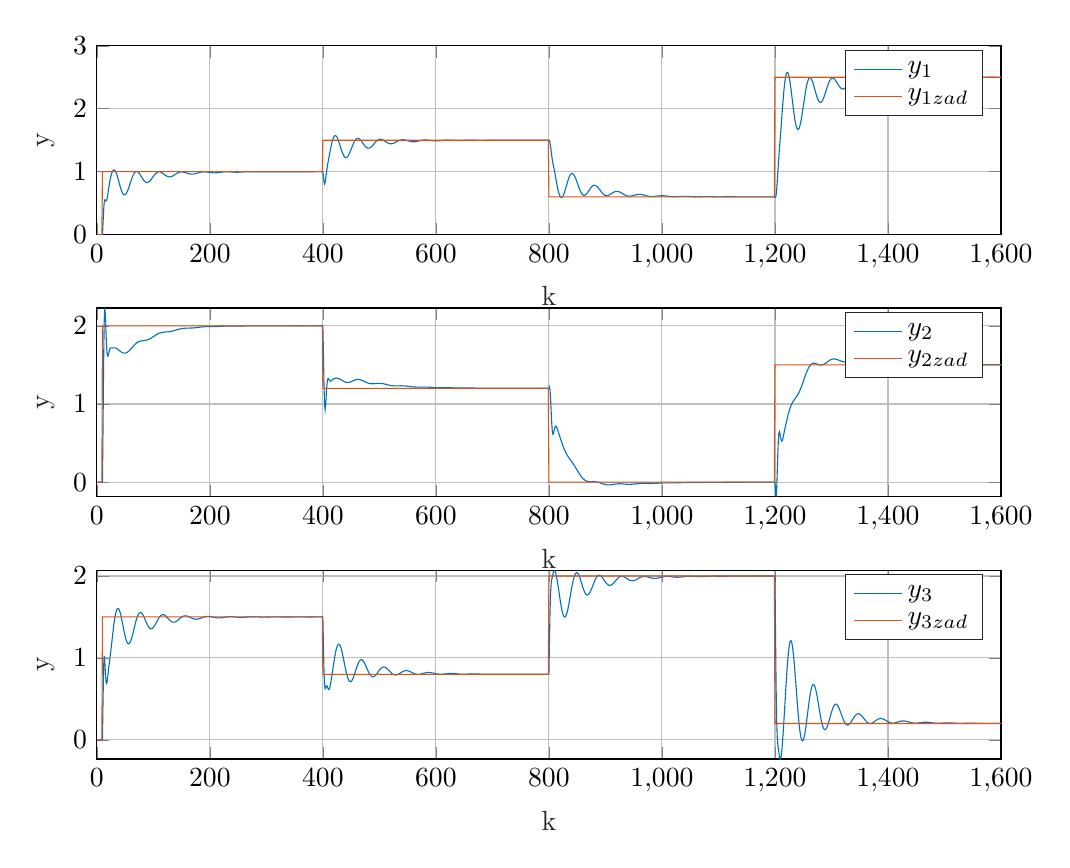
\begin{tikzpicture}

\begin{axis}[%
width=4.521in,
height=0.944in,
at={(0.758in,3.103in)},
scale only axis,
xmin=0,
xmax=1600,
xlabel style={font=\color{white!15!black}},
xlabel={k},
ymin=0,
ymax=3,
ylabel style={font=\color{white!15!black}},
ylabel={y},
axis background/.style={fill=white},
xmajorgrids,
ymajorgrids,
legend style={legend cell align=left, align=left, draw=white!15!black}
]
\addplot [color=mycolor1]
  table[row sep=crcr]{%
1	0\\
2	0\\
3	0\\
4	0\\
5	0\\
6	0\\
7	0\\
8	0\\
9	0\\
10	0\\
11	0.17767\\
12	0.3739\\
13	0.50306\\
14	0.55253\\
15	0.55135\\
16	0.53746\\
17	0.53776\\
18	0.56251\\
19	0.60903\\
20	0.6685\\
21	0.73169\\
22	0.79197\\
23	0.8459\\
24	0.89247\\
25	0.93183\\
26	0.96443\\
27	0.99051\\
28	1.01\\
29	1.0228\\
30	1.0288\\
31	1.0278\\
32	1.0204\\
33	1.0068\\
34	0.98775\\
35	0.96406\\
36	0.93658\\
37	0.90624\\
38	0.87398\\
39	0.84078\\
40	0.80756\\
41	0.77524\\
42	0.74466\\
43	0.71659\\
44	0.69172\\
45	0.67062\\
46	0.65375\\
47	0.64145\\
48	0.63393\\
49	0.63125\\
50	0.63339\\
51	0.64019\\
52	0.65136\\
53	0.66654\\
54	0.68528\\
55	0.70704\\
56	0.73125\\
57	0.75728\\
58	0.78449\\
59	0.81224\\
60	0.83987\\
61	0.86678\\
62	0.8924\\
63	0.91622\\
64	0.93776\\
65	0.95666\\
66	0.97261\\
67	0.98539\\
68	0.99487\\
69	1.001\\
70	1.0038\\
71	1.0034\\
72	1\\
73	0.99384\\
74	0.98523\\
75	0.97454\\
76	0.96215\\
77	0.9485\\
78	0.93402\\
79	0.91914\\
80	0.90429\\
81	0.8899\\
82	0.87634\\
83	0.86395\\
84	0.85305\\
85	0.84389\\
86	0.83666\\
87	0.83152\\
88	0.82855\\
89	0.82778\\
90	0.82917\\
91	0.83266\\
92	0.83811\\
93	0.84535\\
94	0.85416\\
95	0.8643\\
96	0.87551\\
97	0.88749\\
98	0.89996\\
99	0.91261\\
100	0.92518\\
101	0.93736\\
102	0.94892\\
103	0.95962\\
104	0.96925\\
105	0.97766\\
106	0.9847\\
107	0.99029\\
108	0.99437\\
109	0.99693\\
110	0.99798\\
111	0.99759\\
112	0.99585\\
113	0.99287\\
114	0.9888\\
115	0.98382\\
116	0.9781\\
117	0.97183\\
118	0.96522\\
119	0.95847\\
120	0.95176\\
121	0.94528\\
122	0.93922\\
123	0.93371\\
124	0.9289\\
125	0.9249\\
126	0.92179\\
127	0.91964\\
128	0.91848\\
129	0.91833\\
130	0.91915\\
131	0.92093\\
132	0.92358\\
133	0.92703\\
134	0.93118\\
135	0.93592\\
136	0.94112\\
137	0.94666\\
138	0.9524\\
139	0.9582\\
140	0.96393\\
141	0.96948\\
142	0.97472\\
143	0.97956\\
144	0.98389\\
145	0.98766\\
146	0.9908\\
147	0.99328\\
148	0.99506\\
149	0.99615\\
150	0.99656\\
151	0.99632\\
152	0.99547\\
153	0.99407\\
154	0.99219\\
155	0.9899\\
156	0.98729\\
157	0.98445\\
158	0.98146\\
159	0.97842\\
160	0.97542\\
161	0.97254\\
162	0.96985\\
163	0.96743\\
164	0.96534\\
165	0.96362\\
166	0.96231\\
167	0.96144\\
168	0.96102\\
169	0.96106\\
170	0.96154\\
171	0.96245\\
172	0.96375\\
173	0.96541\\
174	0.96738\\
175	0.96961\\
176	0.97204\\
177	0.9746\\
178	0.97725\\
179	0.97992\\
180	0.98255\\
181	0.98509\\
182	0.98748\\
183	0.98967\\
184	0.99164\\
185	0.99333\\
186	0.99474\\
187	0.99584\\
188	0.99663\\
189	0.9971\\
190	0.99727\\
191	0.99714\\
192	0.99673\\
193	0.99608\\
194	0.99522\\
195	0.99417\\
196	0.99299\\
197	0.9917\\
198	0.99036\\
199	0.989\\
200	0.98766\\
201	0.98638\\
202	0.9852\\
203	0.98414\\
204	0.98323\\
205	0.9825\\
206	0.98195\\
207	0.98161\\
208	0.98147\\
209	0.98154\\
210	0.98181\\
211	0.98227\\
212	0.98291\\
213	0.9837\\
214	0.98464\\
215	0.98568\\
216	0.98682\\
217	0.98801\\
218	0.98923\\
219	0.99046\\
220	0.99167\\
221	0.99282\\
222	0.99391\\
223	0.99491\\
224	0.9958\\
225	0.99656\\
226	0.99719\\
227	0.99768\\
228	0.99803\\
229	0.99823\\
230	0.9983\\
231	0.99823\\
232	0.99804\\
233	0.99773\\
234	0.99734\\
235	0.99686\\
236	0.99632\\
237	0.99574\\
238	0.99514\\
239	0.99453\\
240	0.99393\\
241	0.99336\\
242	0.99284\\
243	0.99238\\
244	0.99199\\
245	0.99167\\
246	0.99145\\
247	0.99132\\
248	0.99128\\
249	0.99133\\
250	0.99147\\
251	0.9917\\
252	0.99201\\
253	0.99239\\
254	0.99283\\
255	0.99332\\
256	0.99385\\
257	0.9944\\
258	0.99497\\
259	0.99553\\
260	0.99608\\
261	0.99661\\
262	0.9971\\
263	0.99755\\
264	0.99795\\
265	0.9983\\
266	0.99858\\
267	0.9988\\
268	0.99895\\
269	0.99904\\
270	0.99906\\
271	0.99902\\
272	0.99893\\
273	0.99879\\
274	0.99861\\
275	0.99839\\
276	0.99814\\
277	0.99788\\
278	0.99761\\
279	0.99734\\
280	0.99707\\
281	0.99682\\
282	0.99659\\
283	0.99638\\
284	0.99621\\
285	0.99608\\
286	0.99599\\
287	0.99594\\
288	0.99593\\
289	0.99596\\
290	0.99604\\
291	0.99615\\
292	0.9963\\
293	0.99648\\
294	0.99669\\
295	0.99691\\
296	0.99716\\
297	0.99741\\
298	0.99767\\
299	0.99793\\
300	0.99818\\
301	0.99842\\
302	0.99865\\
303	0.99885\\
304	0.99903\\
305	0.99918\\
306	0.99931\\
307	0.9994\\
308	0.99947\\
309	0.99951\\
310	0.99951\\
311	0.9995\\
312	0.99945\\
313	0.99939\\
314	0.9993\\
315	0.9992\\
316	0.99909\\
317	0.99897\\
318	0.99885\\
319	0.99872\\
320	0.9986\\
321	0.99849\\
322	0.99839\\
323	0.9983\\
324	0.99823\\
325	0.99817\\
326	0.99813\\
327	0.99811\\
328	0.99811\\
329	0.99813\\
330	0.99817\\
331	0.99823\\
332	0.9983\\
333	0.99838\\
334	0.99848\\
335	0.99859\\
336	0.9987\\
337	0.99882\\
338	0.99893\\
339	0.99905\\
340	0.99917\\
341	0.99928\\
342	0.99938\\
343	0.99947\\
344	0.99956\\
345	0.99963\\
346	0.99969\\
347	0.99973\\
348	0.99976\\
349	0.99978\\
350	0.99979\\
351	0.99978\\
352	0.99976\\
353	0.99974\\
354	0.9997\\
355	0.99966\\
356	0.99961\\
357	0.99956\\
358	0.99951\\
359	0.99946\\
360	0.99941\\
361	0.99936\\
362	0.99932\\
363	0.99928\\
364	0.99924\\
365	0.99922\\
366	0.9992\\
367	0.99919\\
368	0.99919\\
369	0.99919\\
370	0.99921\\
371	0.99923\\
372	0.99925\\
373	0.99928\\
374	0.99932\\
375	0.99936\\
376	0.9994\\
377	0.99945\\
378	0.99949\\
379	0.99954\\
380	0.99958\\
381	0.99963\\
382	0.99967\\
383	0.9997\\
384	0.99974\\
385	0.99977\\
386	0.99979\\
387	0.99981\\
388	0.99983\\
389	0.99984\\
390	0.99984\\
391	0.99984\\
392	0.99984\\
393	0.99984\\
394	0.99983\\
395	0.99982\\
396	0.9998\\
397	0.99979\\
398	0.99977\\
399	0.99976\\
400	0.99974\\
401	0.91807\\
402	0.83857\\
403	0.80661\\
404	0.82793\\
405	0.8854\\
406	0.95709\\
407	1.0272\\
408	1.0889\\
409	1.1423\\
410	1.1909\\
411	1.2379\\
412	1.285\\
413	1.3322\\
414	1.3785\\
415	1.4221\\
416	1.4615\\
417	1.4957\\
418	1.5238\\
419	1.5457\\
420	1.5611\\
421	1.5702\\
422	1.573\\
423	1.5699\\
424	1.5613\\
425	1.5477\\
426	1.5296\\
427	1.5077\\
428	1.4828\\
429	1.4557\\
430	1.4273\\
431	1.3982\\
432	1.3694\\
433	1.3416\\
434	1.3155\\
435	1.2918\\
436	1.271\\
437	1.2535\\
438	1.2398\\
439	1.23\\
440	1.2244\\
441	1.2229\\
442	1.2255\\
443	1.232\\
444	1.2422\\
445	1.2556\\
446	1.272\\
447	1.2908\\
448	1.3115\\
449	1.3336\\
450	1.3565\\
451	1.3798\\
452	1.4027\\
453	1.4249\\
454	1.4458\\
455	1.4651\\
456	1.4823\\
457	1.4972\\
458	1.5095\\
459	1.519\\
460	1.5257\\
461	1.5296\\
462	1.5306\\
463	1.529\\
464	1.5249\\
465	1.5185\\
466	1.5102\\
467	1.5002\\
468	1.4888\\
469	1.4766\\
470	1.4637\\
471	1.4506\\
472	1.4377\\
473	1.4253\\
474	1.4137\\
475	1.4032\\
476	1.3941\\
477	1.3865\\
478	1.3806\\
479	1.3766\\
480	1.3744\\
481	1.3741\\
482	1.3757\\
483	1.379\\
484	1.3839\\
485	1.3903\\
486	1.398\\
487	1.4068\\
488	1.4164\\
489	1.4265\\
490	1.4371\\
491	1.4476\\
492	1.4581\\
493	1.4681\\
494	1.4776\\
495	1.4862\\
496	1.4939\\
497	1.5005\\
498	1.506\\
499	1.5101\\
500	1.513\\
501	1.5145\\
502	1.5148\\
503	1.5139\\
504	1.5119\\
505	1.5089\\
506	1.5049\\
507	1.5003\\
508	1.4951\\
509	1.4894\\
510	1.4835\\
511	1.4776\\
512	1.4718\\
513	1.4662\\
514	1.461\\
515	1.4563\\
516	1.4523\\
517	1.4489\\
518	1.4464\\
519	1.4447\\
520	1.4438\\
521	1.4438\\
522	1.4447\\
523	1.4463\\
524	1.4487\\
525	1.4517\\
526	1.4553\\
527	1.4593\\
528	1.4637\\
529	1.4684\\
530	1.4732\\
531	1.478\\
532	1.4827\\
533	1.4872\\
534	1.4915\\
535	1.4953\\
536	1.4987\\
537	1.5016\\
538	1.504\\
539	1.5058\\
540	1.507\\
541	1.5076\\
542	1.5076\\
543	1.5071\\
544	1.5061\\
545	1.5046\\
546	1.5028\\
547	1.5006\\
548	1.4982\\
549	1.4956\\
550	1.4929\\
551	1.4902\\
552	1.4875\\
553	1.485\\
554	1.4827\\
555	1.4806\\
556	1.4788\\
557	1.4773\\
558	1.4762\\
559	1.4755\\
560	1.4751\\
561	1.4752\\
562	1.4756\\
563	1.4764\\
564	1.4775\\
565	1.4789\\
566	1.4806\\
567	1.4824\\
568	1.4845\\
569	1.4866\\
570	1.4888\\
571	1.4909\\
572	1.4931\\
573	1.4951\\
574	1.497\\
575	1.4987\\
576	1.5002\\
577	1.5015\\
578	1.5025\\
579	1.5033\\
580	1.5038\\
581	1.504\\
582	1.5039\\
583	1.5037\\
584	1.5032\\
585	1.5025\\
586	1.5016\\
587	1.5006\\
588	1.4994\\
589	1.4982\\
590	1.497\\
591	1.4958\\
592	1.4945\\
593	1.4934\\
594	1.4923\\
595	1.4914\\
596	1.4906\\
597	1.49\\
598	1.4895\\
599	1.4892\\
600	1.489\\
601	1.4891\\
602	1.4893\\
603	1.4897\\
604	1.4902\\
605	1.4908\\
606	1.4916\\
607	1.4925\\
608	1.4934\\
609	1.4944\\
610	1.4953\\
611	1.4963\\
612	1.4973\\
613	1.4982\\
614	1.499\\
615	1.4998\\
616	1.5005\\
617	1.501\\
618	1.5015\\
619	1.5018\\
620	1.502\\
621	1.5021\\
622	1.502\\
623	1.5019\\
624	1.5016\\
625	1.5013\\
626	1.5009\\
627	1.5004\\
628	1.4999\\
629	1.4993\\
630	1.4987\\
631	1.4982\\
632	1.4976\\
633	1.4971\\
634	1.4966\\
635	1.4962\\
636	1.4959\\
637	1.4956\\
638	1.4954\\
639	1.4952\\
640	1.4952\\
641	1.4952\\
642	1.4953\\
643	1.4955\\
644	1.4957\\
645	1.496\\
646	1.4964\\
647	1.4968\\
648	1.4972\\
649	1.4976\\
650	1.4981\\
651	1.4985\\
652	1.499\\
653	1.4994\\
654	1.4997\\
655	1.5001\\
656	1.5004\\
657	1.5006\\
658	1.5008\\
659	1.5009\\
660	1.501\\
661	1.501\\
662	1.501\\
663	1.5009\\
664	1.5008\\
665	1.5007\\
666	1.5005\\
667	1.5002\\
668	1.5\\
669	1.4997\\
670	1.4995\\
671	1.4992\\
672	1.499\\
673	1.4987\\
674	1.4985\\
675	1.4983\\
676	1.4982\\
677	1.498\\
678	1.498\\
679	1.4979\\
680	1.4979\\
681	1.4979\\
682	1.498\\
683	1.498\\
684	1.4982\\
685	1.4983\\
686	1.4985\\
687	1.4986\\
688	1.4988\\
689	1.499\\
690	1.4992\\
691	1.4994\\
692	1.4996\\
693	1.4998\\
694	1.5\\
695	1.5001\\
696	1.5002\\
697	1.5004\\
698	1.5004\\
699	1.5005\\
700	1.5005\\
701	1.5005\\
702	1.5005\\
703	1.5005\\
704	1.5004\\
705	1.5003\\
706	1.5002\\
707	1.5001\\
708	1.5\\
709	1.4999\\
710	1.4998\\
711	1.4997\\
712	1.4996\\
713	1.4994\\
714	1.4994\\
715	1.4993\\
716	1.4992\\
717	1.4991\\
718	1.4991\\
719	1.4991\\
720	1.4991\\
721	1.4991\\
722	1.4991\\
723	1.4991\\
724	1.4992\\
725	1.4993\\
726	1.4993\\
727	1.4994\\
728	1.4995\\
729	1.4996\\
730	1.4997\\
731	1.4998\\
732	1.4999\\
733	1.5\\
734	1.5\\
735	1.5001\\
736	1.5002\\
737	1.5002\\
738	1.5002\\
739	1.5003\\
740	1.5003\\
741	1.5003\\
742	1.5003\\
743	1.5003\\
744	1.5002\\
745	1.5002\\
746	1.5002\\
747	1.5001\\
748	1.5001\\
749	1.5\\
750	1.5\\
751	1.4999\\
752	1.4999\\
753	1.4998\\
754	1.4998\\
755	1.4997\\
756	1.4997\\
757	1.4997\\
758	1.4997\\
759	1.4996\\
760	1.4996\\
761	1.4996\\
762	1.4996\\
763	1.4997\\
764	1.4997\\
765	1.4997\\
766	1.4997\\
767	1.4998\\
768	1.4998\\
769	1.4998\\
770	1.4999\\
771	1.4999\\
772	1.4999\\
773	1.5\\
774	1.5\\
775	1.5\\
776	1.5\\
777	1.5001\\
778	1.5001\\
779	1.5001\\
780	1.5001\\
781	1.5001\\
782	1.5001\\
783	1.5001\\
784	1.5001\\
785	1.5001\\
786	1.5001\\
787	1.5\\
788	1.5\\
789	1.5\\
790	1.5\\
791	1.5\\
792	1.5\\
793	1.4999\\
794	1.4999\\
795	1.4999\\
796	1.4999\\
797	1.4999\\
798	1.4999\\
799	1.4999\\
800	1.4999\\
801	1.4911\\
802	1.4588\\
803	1.4005\\
804	1.3278\\
805	1.2551\\
806	1.1919\\
807	1.1398\\
808	1.0951\\
809	1.0524\\
810	1.0076\\
811	0.95922\\
812	0.90781\\
813	0.8554\\
814	0.80433\\
815	0.75666\\
816	0.71389\\
817	0.67695\\
818	0.64636\\
819	0.62239\\
820	0.60514\\
821	0.59463\\
822	0.59073\\
823	0.59323\\
824	0.60177\\
825	0.61585\\
826	0.63486\\
827	0.65808\\
828	0.68469\\
829	0.71384\\
830	0.74464\\
831	0.7762\\
832	0.80764\\
833	0.83811\\
834	0.86684\\
835	0.89312\\
836	0.91631\\
837	0.9359\\
838	0.95148\\
839	0.96274\\
840	0.96951\\
841	0.97172\\
842	0.96943\\
843	0.9628\\
844	0.9521\\
845	0.93768\\
846	0.91997\\
847	0.89948\\
848	0.87675\\
849	0.85237\\
850	0.82694\\
851	0.80106\\
852	0.77533\\
853	0.75032\\
854	0.72655\\
855	0.70451\\
856	0.68461\\
857	0.6672\\
858	0.65255\\
859	0.64086\\
860	0.63225\\
861	0.62676\\
862	0.62434\\
863	0.62487\\
864	0.62818\\
865	0.63402\\
866	0.6421\\
867	0.65207\\
868	0.66356\\
869	0.67618\\
870	0.68952\\
871	0.70318\\
872	0.71674\\
873	0.72984\\
874	0.74212\\
875	0.75325\\
876	0.76296\\
877	0.77103\\
878	0.77725\\
879	0.78152\\
880	0.78375\\
881	0.78392\\
882	0.78207\\
883	0.77827\\
884	0.77266\\
885	0.76539\\
886	0.75669\\
887	0.74676\\
888	0.73587\\
889	0.72428\\
890	0.71227\\
891	0.70012\\
892	0.68808\\
893	0.67642\\
894	0.66538\\
895	0.65516\\
896	0.64596\\
897	0.63792\\
898	0.63116\\
899	0.62577\\
900	0.6218\\
901	0.61925\\
902	0.6181\\
903	0.61829\\
904	0.61974\\
905	0.62233\\
906	0.62592\\
907	0.63035\\
908	0.63546\\
909	0.64105\\
910	0.64695\\
911	0.65297\\
912	0.65892\\
913	0.66465\\
914	0.66998\\
915	0.67477\\
916	0.6789\\
917	0.68228\\
918	0.68481\\
919	0.68645\\
920	0.68717\\
921	0.68695\\
922	0.68583\\
923	0.68383\\
924	0.68102\\
925	0.67748\\
926	0.6733\\
927	0.66859\\
928	0.66346\\
929	0.65804\\
930	0.65246\\
931	0.64683\\
932	0.64127\\
933	0.63592\\
934	0.63086\\
935	0.62619\\
936	0.622\\
937	0.61836\\
938	0.61531\\
939	0.61289\\
940	0.61111\\
941	0.60999\\
942	0.6095\\
943	0.60963\\
944	0.61032\\
945	0.61151\\
946	0.61316\\
947	0.61518\\
948	0.61749\\
949	0.62002\\
950	0.62267\\
951	0.62537\\
952	0.62802\\
953	0.63056\\
954	0.63291\\
955	0.63501\\
956	0.6368\\
957	0.63824\\
958	0.6393\\
959	0.63994\\
960	0.64017\\
961	0.63998\\
962	0.63937\\
963	0.63837\\
964	0.63701\\
965	0.63532\\
966	0.63335\\
967	0.63115\\
968	0.62877\\
969	0.62627\\
970	0.6237\\
971	0.62112\\
972	0.61859\\
973	0.61615\\
974	0.61386\\
975	0.61176\\
976	0.60987\\
977	0.60824\\
978	0.60689\\
979	0.60582\\
980	0.60505\\
981	0.60457\\
982	0.60439\\
983	0.60448\\
984	0.60482\\
985	0.60539\\
986	0.60616\\
987	0.60709\\
988	0.60816\\
989	0.60931\\
990	0.61052\\
991	0.61173\\
992	0.61293\\
993	0.61407\\
994	0.61511\\
995	0.61604\\
996	0.61683\\
997	0.61745\\
998	0.6179\\
999	0.61816\\
1000	0.61822\\
1001	0.6181\\
1002	0.61779\\
1003	0.6173\\
1004	0.61666\\
1005	0.61586\\
1006	0.61495\\
1007	0.61393\\
1008	0.61283\\
1009	0.61168\\
1010	0.61051\\
1011	0.60934\\
1012	0.60819\\
1013	0.60709\\
1014	0.60605\\
1015	0.60511\\
1016	0.60427\\
1017	0.60355\\
1018	0.60295\\
1019	0.60248\\
1020	0.60215\\
1021	0.60196\\
1022	0.60189\\
1023	0.60195\\
1024	0.60213\\
1025	0.6024\\
1026	0.60277\\
1027	0.6032\\
1028	0.60369\\
1029	0.60422\\
1030	0.60477\\
1031	0.60533\\
1032	0.60587\\
1033	0.60638\\
1034	0.60685\\
1035	0.60726\\
1036	0.60761\\
1037	0.60788\\
1038	0.60807\\
1039	0.60817\\
1040	0.60819\\
1041	0.60812\\
1042	0.60797\\
1043	0.60773\\
1044	0.60743\\
1045	0.60706\\
1046	0.60663\\
1047	0.60616\\
1048	0.60566\\
1049	0.60514\\
1050	0.6046\\
1051	0.60407\\
1052	0.60355\\
1053	0.60305\\
1054	0.60259\\
1055	0.60217\\
1056	0.6018\\
1057	0.60148\\
1058	0.60122\\
1059	0.60101\\
1060	0.60088\\
1061	0.6008\\
1062	0.60078\\
1063	0.60081\\
1064	0.6009\\
1065	0.60104\\
1066	0.60121\\
1067	0.60141\\
1068	0.60164\\
1069	0.60188\\
1070	0.60214\\
1071	0.60239\\
1072	0.60263\\
1073	0.60286\\
1074	0.60307\\
1075	0.60326\\
1076	0.60341\\
1077	0.60353\\
1078	0.60361\\
1079	0.60365\\
1080	0.60366\\
1081	0.60362\\
1082	0.60354\\
1083	0.60343\\
1084	0.60329\\
1085	0.60312\\
1086	0.60292\\
1087	0.6027\\
1088	0.60247\\
1089	0.60224\\
1090	0.60199\\
1091	0.60175\\
1092	0.60152\\
1093	0.6013\\
1094	0.60109\\
1095	0.6009\\
1096	0.60074\\
1097	0.60059\\
1098	0.60048\\
1099	0.60039\\
1100	0.60034\\
1101	0.60031\\
1102	0.6003\\
1103	0.60032\\
1104	0.60037\\
1105	0.60043\\
1106	0.60051\\
1107	0.60061\\
1108	0.60072\\
1109	0.60083\\
1110	0.60094\\
1111	0.60106\\
1112	0.60117\\
1113	0.60127\\
1114	0.60137\\
1115	0.60145\\
1116	0.60152\\
1117	0.60157\\
1118	0.60161\\
1119	0.60162\\
1120	0.60162\\
1121	0.6016\\
1122	0.60157\\
1123	0.60151\\
1124	0.60145\\
1125	0.60137\\
1126	0.60128\\
1127	0.60118\\
1128	0.60107\\
1129	0.60096\\
1130	0.60085\\
1131	0.60074\\
1132	0.60064\\
1133	0.60054\\
1134	0.60044\\
1135	0.60036\\
1136	0.60028\\
1137	0.60022\\
1138	0.60017\\
1139	0.60013\\
1140	0.6001\\
1141	0.60009\\
1142	0.60009\\
1143	0.60009\\
1144	0.60011\\
1145	0.60014\\
1146	0.60017\\
1147	0.60022\\
1148	0.60026\\
1149	0.60031\\
1150	0.60036\\
1151	0.60041\\
1152	0.60046\\
1153	0.6005\\
1154	0.60054\\
1155	0.60058\\
1156	0.60061\\
1157	0.60063\\
1158	0.60065\\
1159	0.60066\\
1160	0.60066\\
1161	0.60066\\
1162	0.60064\\
1163	0.60062\\
1164	0.6006\\
1165	0.60057\\
1166	0.60054\\
1167	0.6005\\
1168	0.60046\\
1169	0.60042\\
1170	0.60037\\
1171	0.60033\\
1172	0.60029\\
1173	0.60025\\
1174	0.60022\\
1175	0.60018\\
1176	0.60015\\
1177	0.60013\\
1178	0.60011\\
1179	0.60009\\
1180	0.60008\\
1181	0.60007\\
1182	0.60007\\
1183	0.60007\\
1184	0.60007\\
1185	0.60008\\
1186	0.60009\\
1187	0.6001\\
1188	0.60012\\
1189	0.60013\\
1190	0.60015\\
1191	0.60016\\
1192	0.60018\\
1193	0.60019\\
1194	0.60021\\
1195	0.60022\\
1196	0.60023\\
1197	0.60024\\
1198	0.60024\\
1199	0.60025\\
1200	0.60025\\
1201	0.5923\\
1202	0.62309\\
1203	0.71023\\
1204	0.8396\\
1205	0.9851\\
1206	1.1262\\
1207	1.2547\\
1208	1.3729\\
1209	1.4874\\
1210	1.6041\\
1211	1.7254\\
1212	1.8501\\
1213	1.9746\\
1214	2.0944\\
1215	2.2055\\
1216	2.3048\\
1217	2.39\\
1218	2.4599\\
1219	2.5139\\
1220	2.5515\\
1221	2.573\\
1222	2.5786\\
1223	2.569\\
1224	2.5452\\
1225	2.5085\\
1226	2.4604\\
1227	2.4027\\
1228	2.3375\\
1229	2.2667\\
1230	2.1926\\
1231	2.1172\\
1232	2.0426\\
1233	1.9708\\
1234	1.9037\\
1235	1.8429\\
1236	1.7897\\
1237	1.7455\\
1238	1.711\\
1239	1.687\\
1240	1.6737\\
1241	1.6713\\
1242	1.6796\\
1243	1.698\\
1244	1.7259\\
1245	1.7624\\
1246	1.8064\\
1247	1.8567\\
1248	1.9119\\
1249	1.9706\\
1250	2.0314\\
1251	2.0928\\
1252	2.1535\\
1253	2.2121\\
1254	2.2673\\
1255	2.3182\\
1256	2.3636\\
1257	2.4029\\
1258	2.4354\\
1259	2.4608\\
1260	2.4787\\
1261	2.4893\\
1262	2.4925\\
1263	2.4888\\
1264	2.4786\\
1265	2.4625\\
1266	2.4414\\
1267	2.4159\\
1268	2.3871\\
1269	2.3559\\
1270	2.3232\\
1271	2.29\\
1272	2.2574\\
1273	2.226\\
1274	2.1969\\
1275	2.1707\\
1276	2.1481\\
1277	2.1295\\
1278	2.1154\\
1279	2.1061\\
1280	2.1017\\
1281	2.1021\\
1282	2.1074\\
1283	2.1172\\
1284	2.1312\\
1285	2.1491\\
1286	2.1702\\
1287	2.1941\\
1288	2.2202\\
1289	2.2477\\
1290	2.276\\
1291	2.3045\\
1292	2.3325\\
1293	2.3594\\
1294	2.3848\\
1295	2.408\\
1296	2.4287\\
1297	2.4466\\
1298	2.4613\\
1299	2.4727\\
1300	2.4807\\
1301	2.4854\\
1302	2.4867\\
1303	2.4849\\
1304	2.4802\\
1305	2.4728\\
1306	2.4632\\
1307	2.4516\\
1308	2.4386\\
1309	2.4246\\
1310	2.4099\\
1311	2.3951\\
1312	2.3806\\
1313	2.3668\\
1314	2.354\\
1315	2.3425\\
1316	2.3328\\
1317	2.3249\\
1318	2.319\\
1319	2.3154\\
1320	2.3139\\
1321	2.3147\\
1322	2.3176\\
1323	2.3226\\
1324	2.3294\\
1325	2.338\\
1326	2.348\\
1327	2.3592\\
1328	2.3713\\
1329	2.3841\\
1330	2.3972\\
1331	2.4102\\
1332	2.4231\\
1333	2.4354\\
1334	2.4469\\
1335	2.4574\\
1336	2.4667\\
1337	2.4747\\
1338	2.4813\\
1339	2.4863\\
1340	2.4898\\
1341	2.4918\\
1342	2.4923\\
1343	2.4913\\
1344	2.489\\
1345	2.4856\\
1346	2.4811\\
1347	2.4758\\
1348	2.4699\\
1349	2.4635\\
1350	2.4569\\
1351	2.4502\\
1352	2.4437\\
1353	2.4375\\
1354	2.4318\\
1355	2.4268\\
1356	2.4225\\
1357	2.4191\\
1358	2.4167\\
1359	2.4152\\
1360	2.4148\\
1361	2.4153\\
1362	2.4168\\
1363	2.4193\\
1364	2.4226\\
1365	2.4266\\
1366	2.4313\\
1367	2.4365\\
1368	2.4421\\
1369	2.448\\
1370	2.4539\\
1371	2.4599\\
1372	2.4657\\
1373	2.4713\\
1374	2.4765\\
1375	2.4812\\
1376	2.4854\\
1377	2.489\\
1378	2.4919\\
1379	2.4941\\
1380	2.4955\\
1381	2.4963\\
1382	2.4965\\
1383	2.4959\\
1384	2.4948\\
1385	2.4932\\
1386	2.4911\\
1387	2.4886\\
1388	2.4859\\
1389	2.483\\
1390	2.48\\
1391	2.477\\
1392	2.474\\
1393	2.4713\\
1394	2.4687\\
1395	2.4665\\
1396	2.4646\\
1397	2.4631\\
1398	2.4621\\
1399	2.4615\\
1400	2.4614\\
1401	2.4617\\
1402	2.4625\\
1403	2.4637\\
1404	2.4652\\
1405	2.4671\\
1406	2.4693\\
1407	2.4717\\
1408	2.4743\\
1409	2.477\\
1410	2.4797\\
1411	2.4824\\
1412	2.485\\
1413	2.4875\\
1414	2.4899\\
1415	2.492\\
1416	2.4938\\
1417	2.4954\\
1418	2.4967\\
1419	2.4976\\
1420	2.4983\\
1421	2.4986\\
1422	2.4986\\
1423	2.4983\\
1424	2.4977\\
1425	2.497\\
1426	2.496\\
1427	2.4948\\
1428	2.4936\\
1429	2.4922\\
1430	2.4909\\
1431	2.4895\\
1432	2.4882\\
1433	2.4869\\
1434	2.4858\\
1435	2.4848\\
1436	2.484\\
1437	2.4833\\
1438	2.4829\\
1439	2.4827\\
1440	2.4826\\
1441	2.4828\\
1442	2.4832\\
1443	2.4838\\
1444	2.4845\\
1445	2.4854\\
1446	2.4864\\
1447	2.4875\\
1448	2.4887\\
1449	2.4899\\
1450	2.4911\\
1451	2.4924\\
1452	2.4936\\
1453	2.4947\\
1454	2.4957\\
1455	2.4967\\
1456	2.4975\\
1457	2.4982\\
1458	2.4987\\
1459	2.4991\\
1460	2.4994\\
1461	2.4995\\
1462	2.4995\\
1463	2.4994\\
1464	2.4991\\
1465	2.4987\\
1466	2.4982\\
1467	2.4977\\
1468	2.4971\\
1469	2.4965\\
1470	2.4959\\
1471	2.4953\\
1472	2.4947\\
1473	2.4941\\
1474	2.4936\\
1475	2.4932\\
1476	2.4928\\
1477	2.4925\\
1478	2.4923\\
1479	2.4922\\
1480	2.4922\\
1481	2.4923\\
1482	2.4925\\
1483	2.4928\\
1484	2.4931\\
1485	2.4935\\
1486	2.494\\
1487	2.4945\\
1488	2.4951\\
1489	2.4956\\
1490	2.4962\\
1491	2.4967\\
1492	2.4973\\
1493	2.4978\\
1494	2.4982\\
1495	2.4987\\
1496	2.499\\
1497	2.4993\\
1498	2.4996\\
1499	2.4997\\
1500	2.4998\\
1501	2.4999\\
1502	2.4999\\
1503	2.4998\\
1504	2.4997\\
1505	2.4995\\
1506	2.4993\\
1507	2.499\\
1508	2.4987\\
1509	2.4985\\
1510	2.4982\\
1511	2.4979\\
1512	2.4976\\
1513	2.4974\\
1514	2.4971\\
1515	2.4969\\
1516	2.4968\\
1517	2.4967\\
1518	2.4966\\
1519	2.4965\\
1520	2.4965\\
1521	2.4966\\
1522	2.4967\\
1523	2.4968\\
1524	2.497\\
1525	2.4972\\
1526	2.4974\\
1527	2.4976\\
1528	2.4979\\
1529	2.4981\\
1530	2.4984\\
1531	2.4986\\
1532	2.4989\\
1533	2.4991\\
1534	2.4993\\
1535	2.4995\\
1536	2.4997\\
1537	2.4998\\
1538	2.4999\\
1539	2.5\\
1540	2.5\\
1541	2.5\\
1542	2.5\\
1543	2.5\\
1544	2.5\\
1545	2.4999\\
1546	2.4998\\
1547	2.4997\\
1548	2.4996\\
1549	2.4994\\
1550	2.4993\\
1551	2.4992\\
1552	2.4991\\
1553	2.499\\
1554	2.4989\\
1555	2.4988\\
1556	2.4987\\
1557	2.4987\\
1558	2.4986\\
1559	2.4986\\
1560	2.4986\\
1561	2.4986\\
1562	2.4986\\
1563	2.4987\\
1564	2.4987\\
1565	2.4988\\
1566	2.4989\\
1567	2.499\\
1568	2.4991\\
1569	2.4992\\
1570	2.4993\\
1571	2.4994\\
1572	2.4995\\
1573	2.4996\\
1574	2.4996\\
1575	2.4997\\
1576	2.4998\\
1577	2.4998\\
1578	2.4999\\
1579	2.4999\\
1580	2.4999\\
1581	2.4999\\
1582	2.4999\\
1583	2.4999\\
1584	2.4999\\
1585	2.4999\\
1586	2.4999\\
1587	2.4998\\
1588	2.4998\\
1589	2.4998\\
1590	2.4997\\
1591	2.4997\\
1592	2.4996\\
1593	2.4996\\
1594	2.4996\\
1595	2.4995\\
1596	2.4995\\
1597	2.4995\\
1598	2.4995\\
1599	2.4995\\
1600	2.4995\\
};
\addlegendentry{$\text{y}_\text{1}$}

\addplot [color=mycolor2]
  table[row sep=crcr]{%
1	0\\
2	0\\
3	0\\
4	0\\
5	0\\
6	0\\
7	0\\
8	0\\
9	0\\
10	1\\
11	1\\
12	1\\
13	1\\
14	1\\
15	1\\
16	1\\
17	1\\
18	1\\
19	1\\
20	1\\
21	1\\
22	1\\
23	1\\
24	1\\
25	1\\
26	1\\
27	1\\
28	1\\
29	1\\
30	1\\
31	1\\
32	1\\
33	1\\
34	1\\
35	1\\
36	1\\
37	1\\
38	1\\
39	1\\
40	1\\
41	1\\
42	1\\
43	1\\
44	1\\
45	1\\
46	1\\
47	1\\
48	1\\
49	1\\
50	1\\
51	1\\
52	1\\
53	1\\
54	1\\
55	1\\
56	1\\
57	1\\
58	1\\
59	1\\
60	1\\
61	1\\
62	1\\
63	1\\
64	1\\
65	1\\
66	1\\
67	1\\
68	1\\
69	1\\
70	1\\
71	1\\
72	1\\
73	1\\
74	1\\
75	1\\
76	1\\
77	1\\
78	1\\
79	1\\
80	1\\
81	1\\
82	1\\
83	1\\
84	1\\
85	1\\
86	1\\
87	1\\
88	1\\
89	1\\
90	1\\
91	1\\
92	1\\
93	1\\
94	1\\
95	1\\
96	1\\
97	1\\
98	1\\
99	1\\
100	1\\
101	1\\
102	1\\
103	1\\
104	1\\
105	1\\
106	1\\
107	1\\
108	1\\
109	1\\
110	1\\
111	1\\
112	1\\
113	1\\
114	1\\
115	1\\
116	1\\
117	1\\
118	1\\
119	1\\
120	1\\
121	1\\
122	1\\
123	1\\
124	1\\
125	1\\
126	1\\
127	1\\
128	1\\
129	1\\
130	1\\
131	1\\
132	1\\
133	1\\
134	1\\
135	1\\
136	1\\
137	1\\
138	1\\
139	1\\
140	1\\
141	1\\
142	1\\
143	1\\
144	1\\
145	1\\
146	1\\
147	1\\
148	1\\
149	1\\
150	1\\
151	1\\
152	1\\
153	1\\
154	1\\
155	1\\
156	1\\
157	1\\
158	1\\
159	1\\
160	1\\
161	1\\
162	1\\
163	1\\
164	1\\
165	1\\
166	1\\
167	1\\
168	1\\
169	1\\
170	1\\
171	1\\
172	1\\
173	1\\
174	1\\
175	1\\
176	1\\
177	1\\
178	1\\
179	1\\
180	1\\
181	1\\
182	1\\
183	1\\
184	1\\
185	1\\
186	1\\
187	1\\
188	1\\
189	1\\
190	1\\
191	1\\
192	1\\
193	1\\
194	1\\
195	1\\
196	1\\
197	1\\
198	1\\
199	1\\
200	1\\
201	1\\
202	1\\
203	1\\
204	1\\
205	1\\
206	1\\
207	1\\
208	1\\
209	1\\
210	1\\
211	1\\
212	1\\
213	1\\
214	1\\
215	1\\
216	1\\
217	1\\
218	1\\
219	1\\
220	1\\
221	1\\
222	1\\
223	1\\
224	1\\
225	1\\
226	1\\
227	1\\
228	1\\
229	1\\
230	1\\
231	1\\
232	1\\
233	1\\
234	1\\
235	1\\
236	1\\
237	1\\
238	1\\
239	1\\
240	1\\
241	1\\
242	1\\
243	1\\
244	1\\
245	1\\
246	1\\
247	1\\
248	1\\
249	1\\
250	1\\
251	1\\
252	1\\
253	1\\
254	1\\
255	1\\
256	1\\
257	1\\
258	1\\
259	1\\
260	1\\
261	1\\
262	1\\
263	1\\
264	1\\
265	1\\
266	1\\
267	1\\
268	1\\
269	1\\
270	1\\
271	1\\
272	1\\
273	1\\
274	1\\
275	1\\
276	1\\
277	1\\
278	1\\
279	1\\
280	1\\
281	1\\
282	1\\
283	1\\
284	1\\
285	1\\
286	1\\
287	1\\
288	1\\
289	1\\
290	1\\
291	1\\
292	1\\
293	1\\
294	1\\
295	1\\
296	1\\
297	1\\
298	1\\
299	1\\
300	1\\
301	1\\
302	1\\
303	1\\
304	1\\
305	1\\
306	1\\
307	1\\
308	1\\
309	1\\
310	1\\
311	1\\
312	1\\
313	1\\
314	1\\
315	1\\
316	1\\
317	1\\
318	1\\
319	1\\
320	1\\
321	1\\
322	1\\
323	1\\
324	1\\
325	1\\
326	1\\
327	1\\
328	1\\
329	1\\
330	1\\
331	1\\
332	1\\
333	1\\
334	1\\
335	1\\
336	1\\
337	1\\
338	1\\
339	1\\
340	1\\
341	1\\
342	1\\
343	1\\
344	1\\
345	1\\
346	1\\
347	1\\
348	1\\
349	1\\
350	1\\
351	1\\
352	1\\
353	1\\
354	1\\
355	1\\
356	1\\
357	1\\
358	1\\
359	1\\
360	1\\
361	1\\
362	1\\
363	1\\
364	1\\
365	1\\
366	1\\
367	1\\
368	1\\
369	1\\
370	1\\
371	1\\
372	1\\
373	1\\
374	1\\
375	1\\
376	1\\
377	1\\
378	1\\
379	1\\
380	1\\
381	1\\
382	1\\
383	1\\
384	1\\
385	1\\
386	1\\
387	1\\
388	1\\
389	1\\
390	1\\
391	1\\
392	1\\
393	1\\
394	1\\
395	1\\
396	1\\
397	1\\
398	1\\
399	1\\
400	1.5\\
401	1.5\\
402	1.5\\
403	1.5\\
404	1.5\\
405	1.5\\
406	1.5\\
407	1.5\\
408	1.5\\
409	1.5\\
410	1.5\\
411	1.5\\
412	1.5\\
413	1.5\\
414	1.5\\
415	1.5\\
416	1.5\\
417	1.5\\
418	1.5\\
419	1.5\\
420	1.5\\
421	1.5\\
422	1.5\\
423	1.5\\
424	1.5\\
425	1.5\\
426	1.5\\
427	1.5\\
428	1.5\\
429	1.5\\
430	1.5\\
431	1.5\\
432	1.5\\
433	1.5\\
434	1.5\\
435	1.5\\
436	1.5\\
437	1.5\\
438	1.5\\
439	1.5\\
440	1.5\\
441	1.5\\
442	1.5\\
443	1.5\\
444	1.5\\
445	1.5\\
446	1.5\\
447	1.5\\
448	1.5\\
449	1.5\\
450	1.5\\
451	1.5\\
452	1.5\\
453	1.5\\
454	1.5\\
455	1.5\\
456	1.5\\
457	1.5\\
458	1.5\\
459	1.5\\
460	1.5\\
461	1.5\\
462	1.5\\
463	1.5\\
464	1.5\\
465	1.5\\
466	1.5\\
467	1.5\\
468	1.5\\
469	1.5\\
470	1.5\\
471	1.5\\
472	1.5\\
473	1.5\\
474	1.5\\
475	1.5\\
476	1.5\\
477	1.5\\
478	1.5\\
479	1.5\\
480	1.5\\
481	1.5\\
482	1.5\\
483	1.5\\
484	1.5\\
485	1.5\\
486	1.5\\
487	1.5\\
488	1.5\\
489	1.5\\
490	1.5\\
491	1.5\\
492	1.5\\
493	1.5\\
494	1.5\\
495	1.5\\
496	1.5\\
497	1.5\\
498	1.5\\
499	1.5\\
500	1.5\\
501	1.5\\
502	1.5\\
503	1.5\\
504	1.5\\
505	1.5\\
506	1.5\\
507	1.5\\
508	1.5\\
509	1.5\\
510	1.5\\
511	1.5\\
512	1.5\\
513	1.5\\
514	1.5\\
515	1.5\\
516	1.5\\
517	1.5\\
518	1.5\\
519	1.5\\
520	1.5\\
521	1.5\\
522	1.5\\
523	1.5\\
524	1.5\\
525	1.5\\
526	1.5\\
527	1.5\\
528	1.5\\
529	1.5\\
530	1.5\\
531	1.5\\
532	1.5\\
533	1.5\\
534	1.5\\
535	1.5\\
536	1.5\\
537	1.5\\
538	1.5\\
539	1.5\\
540	1.5\\
541	1.5\\
542	1.5\\
543	1.5\\
544	1.5\\
545	1.5\\
546	1.5\\
547	1.5\\
548	1.5\\
549	1.5\\
550	1.5\\
551	1.5\\
552	1.5\\
553	1.5\\
554	1.5\\
555	1.5\\
556	1.5\\
557	1.5\\
558	1.5\\
559	1.5\\
560	1.5\\
561	1.5\\
562	1.5\\
563	1.5\\
564	1.5\\
565	1.5\\
566	1.5\\
567	1.5\\
568	1.5\\
569	1.5\\
570	1.5\\
571	1.5\\
572	1.5\\
573	1.5\\
574	1.5\\
575	1.5\\
576	1.5\\
577	1.5\\
578	1.5\\
579	1.5\\
580	1.5\\
581	1.5\\
582	1.5\\
583	1.5\\
584	1.5\\
585	1.5\\
586	1.5\\
587	1.5\\
588	1.5\\
589	1.5\\
590	1.5\\
591	1.5\\
592	1.5\\
593	1.5\\
594	1.5\\
595	1.5\\
596	1.5\\
597	1.5\\
598	1.5\\
599	1.5\\
600	1.5\\
601	1.5\\
602	1.5\\
603	1.5\\
604	1.5\\
605	1.5\\
606	1.5\\
607	1.5\\
608	1.5\\
609	1.5\\
610	1.5\\
611	1.5\\
612	1.5\\
613	1.5\\
614	1.5\\
615	1.5\\
616	1.5\\
617	1.5\\
618	1.5\\
619	1.5\\
620	1.5\\
621	1.5\\
622	1.5\\
623	1.5\\
624	1.5\\
625	1.5\\
626	1.5\\
627	1.5\\
628	1.5\\
629	1.5\\
630	1.5\\
631	1.5\\
632	1.5\\
633	1.5\\
634	1.5\\
635	1.5\\
636	1.5\\
637	1.5\\
638	1.5\\
639	1.5\\
640	1.5\\
641	1.5\\
642	1.5\\
643	1.5\\
644	1.5\\
645	1.5\\
646	1.5\\
647	1.5\\
648	1.5\\
649	1.5\\
650	1.5\\
651	1.5\\
652	1.5\\
653	1.5\\
654	1.5\\
655	1.5\\
656	1.5\\
657	1.5\\
658	1.5\\
659	1.5\\
660	1.5\\
661	1.5\\
662	1.5\\
663	1.5\\
664	1.5\\
665	1.5\\
666	1.5\\
667	1.5\\
668	1.5\\
669	1.5\\
670	1.5\\
671	1.5\\
672	1.5\\
673	1.5\\
674	1.5\\
675	1.5\\
676	1.5\\
677	1.5\\
678	1.5\\
679	1.5\\
680	1.5\\
681	1.5\\
682	1.5\\
683	1.5\\
684	1.5\\
685	1.5\\
686	1.5\\
687	1.5\\
688	1.5\\
689	1.5\\
690	1.5\\
691	1.5\\
692	1.5\\
693	1.5\\
694	1.5\\
695	1.5\\
696	1.5\\
697	1.5\\
698	1.5\\
699	1.5\\
700	1.5\\
701	1.5\\
702	1.5\\
703	1.5\\
704	1.5\\
705	1.5\\
706	1.5\\
707	1.5\\
708	1.5\\
709	1.5\\
710	1.5\\
711	1.5\\
712	1.5\\
713	1.5\\
714	1.5\\
715	1.5\\
716	1.5\\
717	1.5\\
718	1.5\\
719	1.5\\
720	1.5\\
721	1.5\\
722	1.5\\
723	1.5\\
724	1.5\\
725	1.5\\
726	1.5\\
727	1.5\\
728	1.5\\
729	1.5\\
730	1.5\\
731	1.5\\
732	1.5\\
733	1.5\\
734	1.5\\
735	1.5\\
736	1.5\\
737	1.5\\
738	1.5\\
739	1.5\\
740	1.5\\
741	1.5\\
742	1.5\\
743	1.5\\
744	1.5\\
745	1.5\\
746	1.5\\
747	1.5\\
748	1.5\\
749	1.5\\
750	1.5\\
751	1.5\\
752	1.5\\
753	1.5\\
754	1.5\\
755	1.5\\
756	1.5\\
757	1.5\\
758	1.5\\
759	1.5\\
760	1.5\\
761	1.5\\
762	1.5\\
763	1.5\\
764	1.5\\
765	1.5\\
766	1.5\\
767	1.5\\
768	1.5\\
769	1.5\\
770	1.5\\
771	1.5\\
772	1.5\\
773	1.5\\
774	1.5\\
775	1.5\\
776	1.5\\
777	1.5\\
778	1.5\\
779	1.5\\
780	1.5\\
781	1.5\\
782	1.5\\
783	1.5\\
784	1.5\\
785	1.5\\
786	1.5\\
787	1.5\\
788	1.5\\
789	1.5\\
790	1.5\\
791	1.5\\
792	1.5\\
793	1.5\\
794	1.5\\
795	1.5\\
796	1.5\\
797	1.5\\
798	1.5\\
799	1.5\\
800	0.6\\
801	0.6\\
802	0.6\\
803	0.6\\
804	0.6\\
805	0.6\\
806	0.6\\
807	0.6\\
808	0.6\\
809	0.6\\
810	0.6\\
811	0.6\\
812	0.6\\
813	0.6\\
814	0.6\\
815	0.6\\
816	0.6\\
817	0.6\\
818	0.6\\
819	0.6\\
820	0.6\\
821	0.6\\
822	0.6\\
823	0.6\\
824	0.6\\
825	0.6\\
826	0.6\\
827	0.6\\
828	0.6\\
829	0.6\\
830	0.6\\
831	0.6\\
832	0.6\\
833	0.6\\
834	0.6\\
835	0.6\\
836	0.6\\
837	0.6\\
838	0.6\\
839	0.6\\
840	0.6\\
841	0.6\\
842	0.6\\
843	0.6\\
844	0.6\\
845	0.6\\
846	0.6\\
847	0.6\\
848	0.6\\
849	0.6\\
850	0.6\\
851	0.6\\
852	0.6\\
853	0.6\\
854	0.6\\
855	0.6\\
856	0.6\\
857	0.6\\
858	0.6\\
859	0.6\\
860	0.6\\
861	0.6\\
862	0.6\\
863	0.6\\
864	0.6\\
865	0.6\\
866	0.6\\
867	0.6\\
868	0.6\\
869	0.6\\
870	0.6\\
871	0.6\\
872	0.6\\
873	0.6\\
874	0.6\\
875	0.6\\
876	0.6\\
877	0.6\\
878	0.6\\
879	0.6\\
880	0.6\\
881	0.6\\
882	0.6\\
883	0.6\\
884	0.6\\
885	0.6\\
886	0.6\\
887	0.6\\
888	0.6\\
889	0.6\\
890	0.6\\
891	0.6\\
892	0.6\\
893	0.6\\
894	0.6\\
895	0.6\\
896	0.6\\
897	0.6\\
898	0.6\\
899	0.6\\
900	0.6\\
901	0.6\\
902	0.6\\
903	0.6\\
904	0.6\\
905	0.6\\
906	0.6\\
907	0.6\\
908	0.6\\
909	0.6\\
910	0.6\\
911	0.6\\
912	0.6\\
913	0.6\\
914	0.6\\
915	0.6\\
916	0.6\\
917	0.6\\
918	0.6\\
919	0.6\\
920	0.6\\
921	0.6\\
922	0.6\\
923	0.6\\
924	0.6\\
925	0.6\\
926	0.6\\
927	0.6\\
928	0.6\\
929	0.6\\
930	0.6\\
931	0.6\\
932	0.6\\
933	0.6\\
934	0.6\\
935	0.6\\
936	0.6\\
937	0.6\\
938	0.6\\
939	0.6\\
940	0.6\\
941	0.6\\
942	0.6\\
943	0.6\\
944	0.6\\
945	0.6\\
946	0.6\\
947	0.6\\
948	0.6\\
949	0.6\\
950	0.6\\
951	0.6\\
952	0.6\\
953	0.6\\
954	0.6\\
955	0.6\\
956	0.6\\
957	0.6\\
958	0.6\\
959	0.6\\
960	0.6\\
961	0.6\\
962	0.6\\
963	0.6\\
964	0.6\\
965	0.6\\
966	0.6\\
967	0.6\\
968	0.6\\
969	0.6\\
970	0.6\\
971	0.6\\
972	0.6\\
973	0.6\\
974	0.6\\
975	0.6\\
976	0.6\\
977	0.6\\
978	0.6\\
979	0.6\\
980	0.6\\
981	0.6\\
982	0.6\\
983	0.6\\
984	0.6\\
985	0.6\\
986	0.6\\
987	0.6\\
988	0.6\\
989	0.6\\
990	0.6\\
991	0.6\\
992	0.6\\
993	0.6\\
994	0.6\\
995	0.6\\
996	0.6\\
997	0.6\\
998	0.6\\
999	0.6\\
1000	0.6\\
1001	0.6\\
1002	0.6\\
1003	0.6\\
1004	0.6\\
1005	0.6\\
1006	0.6\\
1007	0.6\\
1008	0.6\\
1009	0.6\\
1010	0.6\\
1011	0.6\\
1012	0.6\\
1013	0.6\\
1014	0.6\\
1015	0.6\\
1016	0.6\\
1017	0.6\\
1018	0.6\\
1019	0.6\\
1020	0.6\\
1021	0.6\\
1022	0.6\\
1023	0.6\\
1024	0.6\\
1025	0.6\\
1026	0.6\\
1027	0.6\\
1028	0.6\\
1029	0.6\\
1030	0.6\\
1031	0.6\\
1032	0.6\\
1033	0.6\\
1034	0.6\\
1035	0.6\\
1036	0.6\\
1037	0.6\\
1038	0.6\\
1039	0.6\\
1040	0.6\\
1041	0.6\\
1042	0.6\\
1043	0.6\\
1044	0.6\\
1045	0.6\\
1046	0.6\\
1047	0.6\\
1048	0.6\\
1049	0.6\\
1050	0.6\\
1051	0.6\\
1052	0.6\\
1053	0.6\\
1054	0.6\\
1055	0.6\\
1056	0.6\\
1057	0.6\\
1058	0.6\\
1059	0.6\\
1060	0.6\\
1061	0.6\\
1062	0.6\\
1063	0.6\\
1064	0.6\\
1065	0.6\\
1066	0.6\\
1067	0.6\\
1068	0.6\\
1069	0.6\\
1070	0.6\\
1071	0.6\\
1072	0.6\\
1073	0.6\\
1074	0.6\\
1075	0.6\\
1076	0.6\\
1077	0.6\\
1078	0.6\\
1079	0.6\\
1080	0.6\\
1081	0.6\\
1082	0.6\\
1083	0.6\\
1084	0.6\\
1085	0.6\\
1086	0.6\\
1087	0.6\\
1088	0.6\\
1089	0.6\\
1090	0.6\\
1091	0.6\\
1092	0.6\\
1093	0.6\\
1094	0.6\\
1095	0.6\\
1096	0.6\\
1097	0.6\\
1098	0.6\\
1099	0.6\\
1100	0.6\\
1101	0.6\\
1102	0.6\\
1103	0.6\\
1104	0.6\\
1105	0.6\\
1106	0.6\\
1107	0.6\\
1108	0.6\\
1109	0.6\\
1110	0.6\\
1111	0.6\\
1112	0.6\\
1113	0.6\\
1114	0.6\\
1115	0.6\\
1116	0.6\\
1117	0.6\\
1118	0.6\\
1119	0.6\\
1120	0.6\\
1121	0.6\\
1122	0.6\\
1123	0.6\\
1124	0.6\\
1125	0.6\\
1126	0.6\\
1127	0.6\\
1128	0.6\\
1129	0.6\\
1130	0.6\\
1131	0.6\\
1132	0.6\\
1133	0.6\\
1134	0.6\\
1135	0.6\\
1136	0.6\\
1137	0.6\\
1138	0.6\\
1139	0.6\\
1140	0.6\\
1141	0.6\\
1142	0.6\\
1143	0.6\\
1144	0.6\\
1145	0.6\\
1146	0.6\\
1147	0.6\\
1148	0.6\\
1149	0.6\\
1150	0.6\\
1151	0.6\\
1152	0.6\\
1153	0.6\\
1154	0.6\\
1155	0.6\\
1156	0.6\\
1157	0.6\\
1158	0.6\\
1159	0.6\\
1160	0.6\\
1161	0.6\\
1162	0.6\\
1163	0.6\\
1164	0.6\\
1165	0.6\\
1166	0.6\\
1167	0.6\\
1168	0.6\\
1169	0.6\\
1170	0.6\\
1171	0.6\\
1172	0.6\\
1173	0.6\\
1174	0.6\\
1175	0.6\\
1176	0.6\\
1177	0.6\\
1178	0.6\\
1179	0.6\\
1180	0.6\\
1181	0.6\\
1182	0.6\\
1183	0.6\\
1184	0.6\\
1185	0.6\\
1186	0.6\\
1187	0.6\\
1188	0.6\\
1189	0.6\\
1190	0.6\\
1191	0.6\\
1192	0.6\\
1193	0.6\\
1194	0.6\\
1195	0.6\\
1196	0.6\\
1197	0.6\\
1198	0.6\\
1199	0.6\\
1200	2.5\\
1201	2.5\\
1202	2.5\\
1203	2.5\\
1204	2.5\\
1205	2.5\\
1206	2.5\\
1207	2.5\\
1208	2.5\\
1209	2.5\\
1210	2.5\\
1211	2.5\\
1212	2.5\\
1213	2.5\\
1214	2.5\\
1215	2.5\\
1216	2.5\\
1217	2.5\\
1218	2.5\\
1219	2.5\\
1220	2.5\\
1221	2.5\\
1222	2.5\\
1223	2.5\\
1224	2.5\\
1225	2.5\\
1226	2.5\\
1227	2.5\\
1228	2.5\\
1229	2.5\\
1230	2.5\\
1231	2.5\\
1232	2.5\\
1233	2.5\\
1234	2.5\\
1235	2.5\\
1236	2.5\\
1237	2.5\\
1238	2.5\\
1239	2.5\\
1240	2.5\\
1241	2.5\\
1242	2.5\\
1243	2.5\\
1244	2.5\\
1245	2.5\\
1246	2.5\\
1247	2.5\\
1248	2.5\\
1249	2.5\\
1250	2.5\\
1251	2.5\\
1252	2.5\\
1253	2.5\\
1254	2.5\\
1255	2.5\\
1256	2.5\\
1257	2.5\\
1258	2.5\\
1259	2.5\\
1260	2.5\\
1261	2.5\\
1262	2.5\\
1263	2.5\\
1264	2.5\\
1265	2.5\\
1266	2.5\\
1267	2.5\\
1268	2.5\\
1269	2.5\\
1270	2.5\\
1271	2.5\\
1272	2.5\\
1273	2.5\\
1274	2.5\\
1275	2.5\\
1276	2.5\\
1277	2.5\\
1278	2.5\\
1279	2.5\\
1280	2.5\\
1281	2.5\\
1282	2.5\\
1283	2.5\\
1284	2.5\\
1285	2.5\\
1286	2.5\\
1287	2.5\\
1288	2.5\\
1289	2.5\\
1290	2.5\\
1291	2.5\\
1292	2.5\\
1293	2.5\\
1294	2.5\\
1295	2.5\\
1296	2.5\\
1297	2.5\\
1298	2.5\\
1299	2.5\\
1300	2.5\\
1301	2.5\\
1302	2.5\\
1303	2.5\\
1304	2.5\\
1305	2.5\\
1306	2.5\\
1307	2.5\\
1308	2.5\\
1309	2.5\\
1310	2.5\\
1311	2.5\\
1312	2.5\\
1313	2.5\\
1314	2.5\\
1315	2.5\\
1316	2.5\\
1317	2.5\\
1318	2.5\\
1319	2.5\\
1320	2.5\\
1321	2.5\\
1322	2.5\\
1323	2.5\\
1324	2.5\\
1325	2.5\\
1326	2.5\\
1327	2.5\\
1328	2.5\\
1329	2.5\\
1330	2.5\\
1331	2.5\\
1332	2.5\\
1333	2.5\\
1334	2.5\\
1335	2.5\\
1336	2.5\\
1337	2.5\\
1338	2.5\\
1339	2.5\\
1340	2.5\\
1341	2.5\\
1342	2.5\\
1343	2.5\\
1344	2.5\\
1345	2.5\\
1346	2.5\\
1347	2.5\\
1348	2.5\\
1349	2.5\\
1350	2.5\\
1351	2.5\\
1352	2.5\\
1353	2.5\\
1354	2.5\\
1355	2.5\\
1356	2.5\\
1357	2.5\\
1358	2.5\\
1359	2.5\\
1360	2.5\\
1361	2.5\\
1362	2.5\\
1363	2.5\\
1364	2.5\\
1365	2.5\\
1366	2.5\\
1367	2.5\\
1368	2.5\\
1369	2.5\\
1370	2.5\\
1371	2.5\\
1372	2.5\\
1373	2.5\\
1374	2.5\\
1375	2.5\\
1376	2.5\\
1377	2.5\\
1378	2.5\\
1379	2.5\\
1380	2.5\\
1381	2.5\\
1382	2.5\\
1383	2.5\\
1384	2.5\\
1385	2.5\\
1386	2.5\\
1387	2.5\\
1388	2.5\\
1389	2.5\\
1390	2.5\\
1391	2.5\\
1392	2.5\\
1393	2.5\\
1394	2.5\\
1395	2.5\\
1396	2.5\\
1397	2.5\\
1398	2.5\\
1399	2.5\\
1400	2.5\\
1401	2.5\\
1402	2.5\\
1403	2.5\\
1404	2.5\\
1405	2.5\\
1406	2.5\\
1407	2.5\\
1408	2.5\\
1409	2.5\\
1410	2.5\\
1411	2.5\\
1412	2.5\\
1413	2.5\\
1414	2.5\\
1415	2.5\\
1416	2.5\\
1417	2.5\\
1418	2.5\\
1419	2.5\\
1420	2.5\\
1421	2.5\\
1422	2.5\\
1423	2.5\\
1424	2.5\\
1425	2.5\\
1426	2.5\\
1427	2.5\\
1428	2.5\\
1429	2.5\\
1430	2.5\\
1431	2.5\\
1432	2.5\\
1433	2.5\\
1434	2.5\\
1435	2.5\\
1436	2.5\\
1437	2.5\\
1438	2.5\\
1439	2.5\\
1440	2.5\\
1441	2.5\\
1442	2.5\\
1443	2.5\\
1444	2.5\\
1445	2.5\\
1446	2.5\\
1447	2.5\\
1448	2.5\\
1449	2.5\\
1450	2.5\\
1451	2.5\\
1452	2.5\\
1453	2.5\\
1454	2.5\\
1455	2.5\\
1456	2.5\\
1457	2.5\\
1458	2.5\\
1459	2.5\\
1460	2.5\\
1461	2.5\\
1462	2.5\\
1463	2.5\\
1464	2.5\\
1465	2.5\\
1466	2.5\\
1467	2.5\\
1468	2.5\\
1469	2.5\\
1470	2.5\\
1471	2.5\\
1472	2.5\\
1473	2.5\\
1474	2.5\\
1475	2.5\\
1476	2.5\\
1477	2.5\\
1478	2.5\\
1479	2.5\\
1480	2.5\\
1481	2.5\\
1482	2.5\\
1483	2.5\\
1484	2.5\\
1485	2.5\\
1486	2.5\\
1487	2.5\\
1488	2.5\\
1489	2.5\\
1490	2.5\\
1491	2.5\\
1492	2.5\\
1493	2.5\\
1494	2.5\\
1495	2.5\\
1496	2.5\\
1497	2.5\\
1498	2.5\\
1499	2.5\\
1500	2.5\\
1501	2.5\\
1502	2.5\\
1503	2.5\\
1504	2.5\\
1505	2.5\\
1506	2.5\\
1507	2.5\\
1508	2.5\\
1509	2.5\\
1510	2.5\\
1511	2.5\\
1512	2.5\\
1513	2.5\\
1514	2.5\\
1515	2.5\\
1516	2.5\\
1517	2.5\\
1518	2.5\\
1519	2.5\\
1520	2.5\\
1521	2.5\\
1522	2.5\\
1523	2.5\\
1524	2.5\\
1525	2.5\\
1526	2.5\\
1527	2.5\\
1528	2.5\\
1529	2.5\\
1530	2.5\\
1531	2.5\\
1532	2.5\\
1533	2.5\\
1534	2.5\\
1535	2.5\\
1536	2.5\\
1537	2.5\\
1538	2.5\\
1539	2.5\\
1540	2.5\\
1541	2.5\\
1542	2.5\\
1543	2.5\\
1544	2.5\\
1545	2.5\\
1546	2.5\\
1547	2.5\\
1548	2.5\\
1549	2.5\\
1550	2.5\\
1551	2.5\\
1552	2.5\\
1553	2.5\\
1554	2.5\\
1555	2.5\\
1556	2.5\\
1557	2.5\\
1558	2.5\\
1559	2.5\\
1560	2.5\\
1561	2.5\\
1562	2.5\\
1563	2.5\\
1564	2.5\\
1565	2.5\\
1566	2.5\\
1567	2.5\\
1568	2.5\\
1569	2.5\\
1570	2.5\\
1571	2.5\\
1572	2.5\\
1573	2.5\\
1574	2.5\\
1575	2.5\\
1576	2.5\\
1577	2.5\\
1578	2.5\\
1579	2.5\\
1580	2.5\\
1581	2.5\\
1582	2.5\\
1583	2.5\\
1584	2.5\\
1585	2.5\\
1586	2.5\\
1587	2.5\\
1588	2.5\\
1589	2.5\\
1590	2.5\\
1591	2.5\\
1592	2.5\\
1593	2.5\\
1594	2.5\\
1595	2.5\\
1596	2.5\\
1597	2.5\\
1598	2.5\\
1599	2.5\\
1600	2.5\\
};
\addlegendentry{$\text{y}_{\text{1zad}}$}

\end{axis}

\begin{axis}[%
width=4.521in,
height=0.944in,
at={(0.758in,1.792in)},
scale only axis,
xmin=0,
xmax=1600,
xlabel style={font=\color{white!15!black}},
xlabel={k},
ymin=-0.18851,
ymax=2.2277,
ylabel style={font=\color{white!15!black}},
ylabel={y},
axis background/.style={fill=white},
xmajorgrids,
ymajorgrids,
legend style={legend cell align=left, align=left, draw=white!15!black}
]
\addplot [color=mycolor1]
  table[row sep=crcr]{%
1	0\\
2	0\\
3	0\\
4	0\\
5	0\\
6	0\\
7	0\\
8	0\\
9	0\\
10	0\\
11	0.69454\\
12	1.4955\\
13	2.0374\\
14	2.2277\\
15	2.1548\\
16	1.9653\\
17	1.7795\\
18	1.6588\\
19	1.6117\\
20	1.6172\\
21	1.6469\\
22	1.6788\\
23	1.7018\\
24	1.7139\\
25	1.718\\
26	1.7179\\
27	1.717\\
28	1.7166\\
29	1.717\\
30	1.7176\\
31	1.7178\\
32	1.7172\\
33	1.7155\\
34	1.7127\\
35	1.709\\
36	1.7046\\
37	1.6997\\
38	1.6943\\
39	1.6888\\
40	1.6831\\
41	1.6775\\
42	1.672\\
43	1.6669\\
44	1.6623\\
45	1.6582\\
46	1.6549\\
47	1.6524\\
48	1.6508\\
49	1.6501\\
50	1.6505\\
51	1.6518\\
52	1.6542\\
53	1.6575\\
54	1.6618\\
55	1.6669\\
56	1.6728\\
57	1.6794\\
58	1.6866\\
59	1.6943\\
60	1.7023\\
61	1.7106\\
62	1.719\\
63	1.7274\\
64	1.7357\\
65	1.7438\\
66	1.7515\\
67	1.7589\\
68	1.7658\\
69	1.7722\\
70	1.7781\\
71	1.7834\\
72	1.7881\\
73	1.7922\\
74	1.7958\\
75	1.7988\\
76	1.8013\\
77	1.8034\\
78	1.8051\\
79	1.8066\\
80	1.8077\\
81	1.8087\\
82	1.8097\\
83	1.8106\\
84	1.8115\\
85	1.8126\\
86	1.8139\\
87	1.8153\\
88	1.8171\\
89	1.8191\\
90	1.8215\\
91	1.8241\\
92	1.8271\\
93	1.8305\\
94	1.8341\\
95	1.8381\\
96	1.8423\\
97	1.8467\\
98	1.8513\\
99	1.856\\
100	1.8608\\
101	1.8656\\
102	1.8704\\
103	1.8752\\
104	1.8798\\
105	1.8842\\
106	1.8885\\
107	1.8925\\
108	1.8963\\
109	1.8998\\
110	1.903\\
111	1.9058\\
112	1.9084\\
113	1.9107\\
114	1.9127\\
115	1.9144\\
116	1.9158\\
117	1.9171\\
118	1.9181\\
119	1.919\\
120	1.9198\\
121	1.9205\\
122	1.9211\\
123	1.9217\\
124	1.9222\\
125	1.9229\\
126	1.9236\\
127	1.9244\\
128	1.9253\\
129	1.9263\\
130	1.9274\\
131	1.9287\\
132	1.9302\\
133	1.9317\\
134	1.9334\\
135	1.9352\\
136	1.9372\\
137	1.9392\\
138	1.9413\\
139	1.9434\\
140	1.9455\\
141	1.9477\\
142	1.9498\\
143	1.9519\\
144	1.9539\\
145	1.9559\\
146	1.9577\\
147	1.9595\\
148	1.9611\\
149	1.9626\\
150	1.9639\\
151	1.9651\\
152	1.9662\\
153	1.9671\\
154	1.9679\\
155	1.9686\\
156	1.9691\\
157	1.9696\\
158	1.9699\\
159	1.9702\\
160	1.9705\\
161	1.9707\\
162	1.9708\\
163	1.971\\
164	1.9712\\
165	1.9714\\
166	1.9716\\
167	1.9719\\
168	1.9722\\
169	1.9725\\
170	1.973\\
171	1.9735\\
172	1.974\\
173	1.9747\\
174	1.9753\\
175	1.9761\\
176	1.9769\\
177	1.9777\\
178	1.9786\\
179	1.9794\\
180	1.9803\\
181	1.9812\\
182	1.9821\\
183	1.9829\\
184	1.9838\\
185	1.9846\\
186	1.9853\\
187	1.986\\
188	1.9866\\
189	1.9872\\
190	1.9878\\
191	1.9882\\
192	1.9886\\
193	1.9889\\
194	1.9892\\
195	1.9894\\
196	1.9896\\
197	1.9897\\
198	1.9898\\
199	1.9899\\
200	1.9899\\
201	1.9899\\
202	1.9899\\
203	1.99\\
204	1.99\\
205	1.99\\
206	1.99\\
207	1.9901\\
208	1.9902\\
209	1.9903\\
210	1.9904\\
211	1.9906\\
212	1.9908\\
213	1.9911\\
214	1.9913\\
215	1.9916\\
216	1.9919\\
217	1.9922\\
218	1.9926\\
219	1.9929\\
220	1.9933\\
221	1.9937\\
222	1.994\\
223	1.9944\\
224	1.9947\\
225	1.995\\
226	1.9953\\
227	1.9956\\
228	1.9958\\
229	1.996\\
230	1.9962\\
231	1.9964\\
232	1.9965\\
233	1.9966\\
234	1.9967\\
235	1.9968\\
236	1.9968\\
237	1.9969\\
238	1.9969\\
239	1.9969\\
240	1.9968\\
241	1.9968\\
242	1.9968\\
243	1.9968\\
244	1.9967\\
245	1.9967\\
246	1.9967\\
247	1.9967\\
248	1.9967\\
249	1.9968\\
250	1.9968\\
251	1.9969\\
252	1.9969\\
253	1.997\\
254	1.9971\\
255	1.9972\\
256	1.9974\\
257	1.9975\\
258	1.9976\\
259	1.9978\\
260	1.9979\\
261	1.998\\
262	1.9982\\
263	1.9983\\
264	1.9985\\
265	1.9986\\
266	1.9987\\
267	1.9988\\
268	1.9989\\
269	1.999\\
270	1.999\\
271	1.9991\\
272	1.9991\\
273	1.9992\\
274	1.9992\\
275	1.9992\\
276	1.9992\\
277	1.9992\\
278	1.9992\\
279	1.9992\\
280	1.9992\\
281	1.9991\\
282	1.9991\\
283	1.9991\\
284	1.9991\\
285	1.9991\\
286	1.999\\
287	1.999\\
288	1.999\\
289	1.999\\
290	1.999\\
291	1.9991\\
292	1.9991\\
293	1.9991\\
294	1.9992\\
295	1.9992\\
296	1.9992\\
297	1.9993\\
298	1.9993\\
299	1.9994\\
300	1.9995\\
301	1.9995\\
302	1.9996\\
303	1.9996\\
304	1.9997\\
305	1.9997\\
306	1.9998\\
307	1.9998\\
308	1.9998\\
309	1.9999\\
310	1.9999\\
311	1.9999\\
312	1.9999\\
313	1.9999\\
314	1.9999\\
315	1.9999\\
316	1.9999\\
317	1.9999\\
318	1.9999\\
319	1.9999\\
320	1.9999\\
321	1.9999\\
322	1.9999\\
323	1.9998\\
324	1.9998\\
325	1.9998\\
326	1.9998\\
327	1.9998\\
328	1.9998\\
329	1.9998\\
330	1.9998\\
331	1.9998\\
332	1.9998\\
333	1.9998\\
334	1.9998\\
335	1.9998\\
336	1.9999\\
337	1.9999\\
338	1.9999\\
339	1.9999\\
340	1.9999\\
341	2\\
342	2\\
343	2\\
344	2\\
345	2\\
346	2.0001\\
347	2.0001\\
348	2.0001\\
349	2.0001\\
350	2.0001\\
351	2.0001\\
352	2.0001\\
353	2.0001\\
354	2.0001\\
355	2.0001\\
356	2.0001\\
357	2.0001\\
358	2.0001\\
359	2.0001\\
360	2.0001\\
361	2.0001\\
362	2.0001\\
363	2.0001\\
364	2.0001\\
365	2\\
366	2\\
367	2\\
368	2\\
369	2\\
370	2\\
371	2\\
372	2\\
373	2\\
374	2\\
375	2\\
376	2\\
377	2\\
378	2\\
379	2\\
380	2\\
381	2\\
382	2\\
383	2\\
384	2.0001\\
385	2.0001\\
386	2.0001\\
387	2.0001\\
388	2.0001\\
389	2.0001\\
390	2.0001\\
391	2.0001\\
392	2.0001\\
393	2.0001\\
394	2.0001\\
395	2.0001\\
396	2.0001\\
397	2.0001\\
398	2.0001\\
399	2.0001\\
400	2.0001\\
401	1.6515\\
402	1.254\\
403	0.99733\\
404	0.92703\\
405	0.9924\\
406	1.1128\\
407	1.224\\
408	1.2948\\
409	1.3233\\
410	1.323\\
411	1.3106\\
412	1.2984\\
413	1.2922\\
414	1.2926\\
415	1.2976\\
416	1.3045\\
417	1.3112\\
418	1.3169\\
419	1.3212\\
420	1.3243\\
421	1.3266\\
422	1.3283\\
423	1.3293\\
424	1.3297\\
425	1.3295\\
426	1.3286\\
427	1.3269\\
428	1.3246\\
429	1.3217\\
430	1.3182\\
431	1.3144\\
432	1.3102\\
433	1.3058\\
434	1.3014\\
435	1.2971\\
436	1.2929\\
437	1.2889\\
438	1.2854\\
439	1.2822\\
440	1.2796\\
441	1.2776\\
442	1.2761\\
443	1.2753\\
444	1.2751\\
445	1.2755\\
446	1.2765\\
447	1.2781\\
448	1.2801\\
449	1.2825\\
450	1.2853\\
451	1.2883\\
452	1.2914\\
453	1.2946\\
454	1.2978\\
455	1.3009\\
456	1.3038\\
457	1.3064\\
458	1.3086\\
459	1.3105\\
460	1.3119\\
461	1.3128\\
462	1.3133\\
463	1.3132\\
464	1.3126\\
465	1.3115\\
466	1.3099\\
467	1.3079\\
468	1.3055\\
469	1.3027\\
470	1.2997\\
471	1.2964\\
472	1.293\\
473	1.2895\\
474	1.286\\
475	1.2825\\
476	1.2791\\
477	1.2758\\
478	1.2728\\
479	1.27\\
480	1.2674\\
481	1.2652\\
482	1.2633\\
483	1.2617\\
484	1.2605\\
485	1.2596\\
486	1.259\\
487	1.2586\\
488	1.2586\\
489	1.2587\\
490	1.2591\\
491	1.2596\\
492	1.2602\\
493	1.2608\\
494	1.2615\\
495	1.2622\\
496	1.2628\\
497	1.2633\\
498	1.2637\\
499	1.2639\\
500	1.2639\\
501	1.2638\\
502	1.2634\\
503	1.2629\\
504	1.2621\\
505	1.2611\\
506	1.2599\\
507	1.2586\\
508	1.2571\\
509	1.2554\\
510	1.2537\\
511	1.2519\\
512	1.25\\
513	1.2481\\
514	1.2462\\
515	1.2443\\
516	1.2425\\
517	1.2408\\
518	1.2392\\
519	1.2377\\
520	1.2364\\
521	1.2352\\
522	1.2341\\
523	1.2333\\
524	1.2325\\
525	1.232\\
526	1.2316\\
527	1.2313\\
528	1.2311\\
529	1.2311\\
530	1.2311\\
531	1.2312\\
532	1.2314\\
533	1.2315\\
534	1.2317\\
535	1.2319\\
536	1.2321\\
537	1.2322\\
538	1.2323\\
539	1.2323\\
540	1.2322\\
541	1.232\\
542	1.2318\\
543	1.2314\\
544	1.231\\
545	1.2304\\
546	1.2298\\
547	1.2291\\
548	1.2284\\
549	1.2276\\
550	1.2267\\
551	1.2258\\
552	1.2249\\
553	1.224\\
554	1.2231\\
555	1.2222\\
556	1.2213\\
557	1.2205\\
558	1.2197\\
559	1.219\\
560	1.2184\\
561	1.2178\\
562	1.2173\\
563	1.2169\\
564	1.2166\\
565	1.2163\\
566	1.2161\\
567	1.2159\\
568	1.2158\\
569	1.2158\\
570	1.2158\\
571	1.2158\\
572	1.2158\\
573	1.2159\\
574	1.216\\
575	1.216\\
576	1.2161\\
577	1.2161\\
578	1.2161\\
579	1.2161\\
580	1.216\\
581	1.2159\\
582	1.2157\\
583	1.2156\\
584	1.2153\\
585	1.2151\\
586	1.2148\\
587	1.2144\\
588	1.2141\\
589	1.2137\\
590	1.2133\\
591	1.2128\\
592	1.2124\\
593	1.212\\
594	1.2115\\
595	1.2111\\
596	1.2107\\
597	1.2103\\
598	1.21\\
599	1.2096\\
600	1.2093\\
601	1.2091\\
602	1.2088\\
603	1.2086\\
604	1.2085\\
605	1.2083\\
606	1.2082\\
607	1.2081\\
608	1.2081\\
609	1.2081\\
610	1.2081\\
611	1.2081\\
612	1.2081\\
613	1.2081\\
614	1.2081\\
615	1.2081\\
616	1.2081\\
617	1.2081\\
618	1.2081\\
619	1.2081\\
620	1.208\\
621	1.208\\
622	1.2079\\
623	1.2078\\
624	1.2077\\
625	1.2075\\
626	1.2074\\
627	1.2072\\
628	1.207\\
629	1.2069\\
630	1.2067\\
631	1.2065\\
632	1.2063\\
633	1.206\\
634	1.2058\\
635	1.2056\\
636	1.2055\\
637	1.2053\\
638	1.2051\\
639	1.2049\\
640	1.2048\\
641	1.2047\\
642	1.2046\\
643	1.2045\\
644	1.2044\\
645	1.2043\\
646	1.2043\\
647	1.2042\\
648	1.2042\\
649	1.2042\\
650	1.2042\\
651	1.2042\\
652	1.2042\\
653	1.2042\\
654	1.2042\\
655	1.2042\\
656	1.2041\\
657	1.2041\\
658	1.2041\\
659	1.2041\\
660	1.2041\\
661	1.204\\
662	1.204\\
663	1.2039\\
664	1.2039\\
665	1.2038\\
666	1.2037\\
667	1.2037\\
668	1.2036\\
669	1.2035\\
670	1.2034\\
671	1.2033\\
672	1.2032\\
673	1.2031\\
674	1.203\\
675	1.2029\\
676	1.2028\\
677	1.2027\\
678	1.2026\\
679	1.2026\\
680	1.2025\\
681	1.2024\\
682	1.2024\\
683	1.2023\\
684	1.2023\\
685	1.2022\\
686	1.2022\\
687	1.2022\\
688	1.2022\\
689	1.2022\\
690	1.2022\\
691	1.2022\\
692	1.2021\\
693	1.2021\\
694	1.2021\\
695	1.2021\\
696	1.2021\\
697	1.2021\\
698	1.2021\\
699	1.2021\\
700	1.2021\\
701	1.2021\\
702	1.202\\
703	1.202\\
704	1.202\\
705	1.2019\\
706	1.2019\\
707	1.2019\\
708	1.2018\\
709	1.2018\\
710	1.2017\\
711	1.2017\\
712	1.2016\\
713	1.2016\\
714	1.2015\\
715	1.2015\\
716	1.2014\\
717	1.2014\\
718	1.2014\\
719	1.2013\\
720	1.2013\\
721	1.2013\\
722	1.2012\\
723	1.2012\\
724	1.2012\\
725	1.2012\\
726	1.2012\\
727	1.2011\\
728	1.2011\\
729	1.2011\\
730	1.2011\\
731	1.2011\\
732	1.2011\\
733	1.2011\\
734	1.2011\\
735	1.2011\\
736	1.2011\\
737	1.2011\\
738	1.2011\\
739	1.2011\\
740	1.2011\\
741	1.201\\
742	1.201\\
743	1.201\\
744	1.201\\
745	1.201\\
746	1.201\\
747	1.2009\\
748	1.2009\\
749	1.2009\\
750	1.2009\\
751	1.2009\\
752	1.2008\\
753	1.2008\\
754	1.2008\\
755	1.2008\\
756	1.2008\\
757	1.2007\\
758	1.2007\\
759	1.2007\\
760	1.2007\\
761	1.2007\\
762	1.2006\\
763	1.2006\\
764	1.2006\\
765	1.2006\\
766	1.2006\\
767	1.2006\\
768	1.2006\\
769	1.2006\\
770	1.2006\\
771	1.2006\\
772	1.2006\\
773	1.2006\\
774	1.2006\\
775	1.2005\\
776	1.2005\\
777	1.2005\\
778	1.2005\\
779	1.2005\\
780	1.2005\\
781	1.2005\\
782	1.2005\\
783	1.2005\\
784	1.2005\\
785	1.2005\\
786	1.2005\\
787	1.2005\\
788	1.2005\\
789	1.2005\\
790	1.2005\\
791	1.2005\\
792	1.2004\\
793	1.2004\\
794	1.2004\\
795	1.2004\\
796	1.2004\\
797	1.2004\\
798	1.2004\\
799	1.2004\\
800	1.2004\\
801	1.2175\\
802	1.1802\\
803	1.0636\\
804	0.90233\\
805	0.75167\\
806	0.65151\\
807	0.6123\\
808	0.62059\\
809	0.65269\\
810	0.68694\\
811	0.71\\
812	0.71749\\
813	0.71123\\
814	0.69571\\
815	0.67539\\
816	0.65335\\
817	0.63116\\
818	0.60923\\
819	0.58747\\
820	0.56569\\
821	0.54386\\
822	0.52211\\
823	0.50068\\
824	0.47985\\
825	0.45985\\
826	0.44086\\
827	0.42296\\
828	0.40617\\
829	0.39048\\
830	0.37584\\
831	0.36217\\
832	0.34936\\
833	0.33731\\
834	0.32591\\
835	0.31501\\
836	0.3045\\
837	0.29426\\
838	0.28415\\
839	0.27409\\
840	0.26397\\
841	0.25371\\
842	0.24326\\
843	0.23257\\
844	0.22163\\
845	0.21042\\
846	0.19897\\
847	0.1873\\
848	0.17546\\
849	0.16351\\
850	0.15152\\
851	0.13956\\
852	0.12773\\
853	0.1161\\
854	0.10478\\
855	0.093834\\
856	0.083355\\
857	0.073417\\
858	0.064087\\
859	0.055421\\
860	0.047464\\
861	0.040249\\
862	0.033796\\
863	0.028112\\
864	0.02319\\
865	0.019009\\
866	0.01554\\
867	0.012738\\
868	0.010551\\
869	0.0089179\\
870	0.0077716\\
871	0.0070391\\
872	0.0066444\\
873	0.0065102\\
874	0.0065594\\
875	0.0067172\\
876	0.0069125\\
877	0.0070792\\
878	0.0071579\\
879	0.0070964\\
880	0.0068511\\
881	0.0063875\\
882	0.0056803\\
883	0.0047137\\
884	0.0034816\\
885	0.0019867\\
886	0.0002406\\
887	-0.0017375\\
888	-0.0039212\\
889	-0.0062784\\
890	-0.0087717\\
891	-0.01136\\
892	-0.014001\\
893	-0.01665\\
894	-0.019261\\
895	-0.021793\\
896	-0.024204\\
897	-0.026455\\
898	-0.028515\\
899	-0.030353\\
900	-0.031947\\
901	-0.03328\\
902	-0.034339\\
903	-0.03512\\
904	-0.035624\\
905	-0.035858\\
906	-0.035835\\
907	-0.035572\\
908	-0.03509\\
909	-0.034417\\
910	-0.033581\\
911	-0.032613\\
912	-0.031546\\
913	-0.030413\\
914	-0.029247\\
915	-0.028081\\
916	-0.026943\\
917	-0.025864\\
918	-0.024866\\
919	-0.023972\\
920	-0.0232\\
921	-0.022564\\
922	-0.022071\\
923	-0.021729\\
924	-0.021538\\
925	-0.021494\\
926	-0.021591\\
927	-0.021818\\
928	-0.022162\\
929	-0.022606\\
930	-0.023133\\
931	-0.023723\\
932	-0.024355\\
933	-0.025008\\
934	-0.02566\\
935	-0.026293\\
936	-0.026885\\
937	-0.027421\\
938	-0.027884\\
939	-0.02826\\
940	-0.02854\\
941	-0.028715\\
942	-0.028779\\
943	-0.028731\\
944	-0.02857\\
945	-0.0283\\
946	-0.027926\\
947	-0.027457\\
948	-0.026901\\
949	-0.026272\\
950	-0.025581\\
951	-0.024843\\
952	-0.024072\\
953	-0.023283\\
954	-0.02249\\
955	-0.021708\\
956	-0.02095\\
957	-0.020228\\
958	-0.019553\\
959	-0.018934\\
960	-0.018379\\
961	-0.017894\\
962	-0.017481\\
963	-0.017143\\
964	-0.01688\\
965	-0.01669\\
966	-0.016569\\
967	-0.016511\\
968	-0.016511\\
969	-0.016561\\
970	-0.016652\\
971	-0.016774\\
972	-0.016919\\
973	-0.017076\\
974	-0.017236\\
975	-0.01739\\
976	-0.017528\\
977	-0.017642\\
978	-0.017726\\
979	-0.017774\\
980	-0.01778\\
981	-0.017741\\
982	-0.017655\\
983	-0.017521\\
984	-0.017338\\
985	-0.017109\\
986	-0.016837\\
987	-0.016524\\
988	-0.016175\\
989	-0.015796\\
990	-0.015393\\
991	-0.014971\\
992	-0.014538\\
993	-0.014099\\
994	-0.013663\\
995	-0.013234\\
996	-0.012819\\
997	-0.012423\\
998	-0.012052\\
999	-0.011708\\
1000	-0.011395\\
1001	-0.011116\\
1002	-0.010872\\
1003	-0.010664\\
1004	-0.010491\\
1005	-0.010352\\
1006	-0.010246\\
1007	-0.01017\\
1008	-0.010121\\
1009	-0.010095\\
1010	-0.010088\\
1011	-0.010097\\
1012	-0.010116\\
1013	-0.010141\\
1014	-0.010167\\
1015	-0.010192\\
1016	-0.010209\\
1017	-0.010216\\
1018	-0.01021\\
1019	-0.010188\\
1020	-0.010148\\
1021	-0.010087\\
1022	-0.010007\\
1023	-0.0099045\\
1024	-0.0097815\\
1025	-0.0096383\\
1026	-0.0094761\\
1027	-0.0092967\\
1028	-0.0091022\\
1029	-0.008895\\
1030	-0.0086778\\
1031	-0.0084535\\
1032	-0.0082251\\
1033	-0.0079955\\
1034	-0.0077678\\
1035	-0.0075447\\
1036	-0.0073289\\
1037	-0.0071228\\
1038	-0.0069285\\
1039	-0.0067477\\
1040	-0.0065818\\
1041	-0.0064319\\
1042	-0.0062985\\
1043	-0.0061818\\
1044	-0.0060817\\
1045	-0.0059976\\
1046	-0.0059286\\
1047	-0.0058734\\
1048	-0.0058307\\
1049	-0.0057988\\
1050	-0.0057757\\
1051	-0.0057595\\
1052	-0.0057482\\
1053	-0.0057397\\
1054	-0.0057321\\
1055	-0.0057233\\
1056	-0.0057116\\
1057	-0.0056953\\
1058	-0.0056731\\
1059	-0.0056438\\
1060	-0.0056064\\
1061	-0.0055602\\
1062	-0.0055048\\
1063	-0.0054401\\
1064	-0.0053663\\
1065	-0.0052836\\
1066	-0.0051927\\
1067	-0.0050944\\
1068	-0.0049896\\
1069	-0.0048796\\
1070	-0.0047655\\
1071	-0.0046486\\
1072	-0.0045303\\
1073	-0.004412\\
1074	-0.004295\\
1075	-0.0041805\\
1076	-0.0040698\\
1077	-0.0039639\\
1078	-0.0038637\\
1079	-0.00377\\
1080	-0.0036835\\
1081	-0.0036044\\
1082	-0.0035331\\
1083	-0.0034696\\
1084	-0.0034139\\
1085	-0.0033655\\
1086	-0.0033241\\
1087	-0.0032892\\
1088	-0.00326\\
1089	-0.0032357\\
1090	-0.0032155\\
1091	-0.0031985\\
1092	-0.0031837\\
1093	-0.0031702\\
1094	-0.0031571\\
1095	-0.0031435\\
1096	-0.0031286\\
1097	-0.0031118\\
1098	-0.0030922\\
1099	-0.0030695\\
1100	-0.0030432\\
1101	-0.0030131\\
1102	-0.0029788\\
1103	-0.0029405\\
1104	-0.0028982\\
1105	-0.002852\\
1106	-0.0028023\\
1107	-0.0027494\\
1108	-0.0026938\\
1109	-0.002636\\
1110	-0.0025766\\
1111	-0.0025161\\
1112	-0.0024552\\
1113	-0.0023945\\
1114	-0.0023346\\
1115	-0.0022761\\
1116	-0.0022195\\
1117	-0.0021653\\
1118	-0.0021138\\
1119	-0.0020655\\
1120	-0.0020205\\
1121	-0.0019791\\
1122	-0.0019413\\
1123	-0.0019072\\
1124	-0.0018766\\
1125	-0.0018495\\
1126	-0.0018255\\
1127	-0.0018045\\
1128	-0.001786\\
1129	-0.0017698\\
1130	-0.0017554\\
1131	-0.0017424\\
1132	-0.0017305\\
1133	-0.0017192\\
1134	-0.0017081\\
1135	-0.0016968\\
1136	-0.001685\\
1137	-0.0016723\\
1138	-0.0016586\\
1139	-0.0016435\\
1140	-0.0016269\\
1141	-0.0016088\\
1142	-0.0015889\\
1143	-0.0015674\\
1144	-0.0015443\\
1145	-0.0015196\\
1146	-0.0014935\\
1147	-0.0014662\\
1148	-0.0014377\\
1149	-0.0014085\\
1150	-0.0013786\\
1151	-0.0013484\\
1152	-0.0013188\\
1153	-0.0012901\\
1154	-0.0012621\\
1155	-0.0012343\\
1156	-0.0012063\\
1157	-0.0011783\\
1158	-0.0011509\\
1159	-0.0011245\\
1160	-0.0010996\\
1161	-0.0010763\\
1162	-0.0010547\\
1163	-0.0010347\\
1164	-0.0010162\\
1165	-0.0009993\\
1166	-0.00098383\\
1167	-0.00096978\\
1168	-0.00095706\\
1169	-0.00094557\\
1170	-0.00093517\\
1171	-0.00092568\\
1172	-0.00091694\\
1173	-0.00090879\\
1174	-0.00090107\\
1175	-0.00089361\\
1176	-0.00088627\\
1177	-0.0008789\\
1178	-0.00087138\\
1179	-0.00086359\\
1180	-0.00085544\\
1181	-0.00084682\\
1182	-0.00083769\\
1183	-0.00082799\\
1184	-0.00081771\\
1185	-0.00080682\\
1186	-0.00079535\\
1187	-0.00078332\\
1188	-0.00077078\\
1189	-0.00075778\\
1190	-0.00074438\\
1191	-0.00073068\\
1192	-0.00071674\\
1193	-0.00070266\\
1194	-0.00068852\\
1195	-0.00067443\\
1196	-0.00066045\\
1197	-0.00064669\\
1198	-0.00063321\\
1199	-0.00062008\\
1200	-0.00060738\\
1201	-0.12545\\
1202	-0.18851\\
1203	-0.097305\\
1204	0.11406\\
1205	0.35242\\
1206	0.53664\\
1207	0.63171\\
1208	0.64666\\
1209	0.61411\\
1210	0.56899\\
1211	0.53548\\
1212	0.52381\\
1213	0.53335\\
1214	0.55796\\
1215	0.59066\\
1216	0.62616\\
1217	0.66154\\
1218	0.69579\\
1219	0.7289\\
1220	0.76115\\
1221	0.79266\\
1222	0.82327\\
1223	0.85268\\
1224	0.88049\\
1225	0.90637\\
1226	0.93013\\
1227	0.95167\\
1228	0.97103\\
1229	0.98834\\
1230	1.0038\\
1231	1.0176\\
1232	1.03\\
1233	1.0414\\
1234	1.0519\\
1235	1.062\\
1236	1.0718\\
1237	1.0818\\
1238	1.0921\\
1239	1.1029\\
1240	1.1146\\
1241	1.1271\\
1242	1.1407\\
1243	1.1554\\
1244	1.1712\\
1245	1.1881\\
1246	1.206\\
1247	1.2248\\
1248	1.2444\\
1249	1.2647\\
1250	1.2853\\
1251	1.3062\\
1252	1.3271\\
1253	1.3478\\
1254	1.368\\
1255	1.3875\\
1256	1.4061\\
1257	1.4237\\
1258	1.4401\\
1259	1.4551\\
1260	1.4686\\
1261	1.4805\\
1262	1.4909\\
1263	1.4996\\
1264	1.5067\\
1265	1.5123\\
1266	1.5164\\
1267	1.5191\\
1268	1.5205\\
1269	1.5208\\
1270	1.5202\\
1271	1.5187\\
1272	1.5167\\
1273	1.5142\\
1274	1.5115\\
1275	1.5087\\
1276	1.5059\\
1277	1.5034\\
1278	1.5013\\
1279	1.4996\\
1280	1.4984\\
1281	1.498\\
1282	1.4981\\
1283	1.4991\\
1284	1.5007\\
1285	1.503\\
1286	1.506\\
1287	1.5096\\
1288	1.5137\\
1289	1.5183\\
1290	1.5233\\
1291	1.5285\\
1292	1.5338\\
1293	1.5393\\
1294	1.5446\\
1295	1.5498\\
1296	1.5547\\
1297	1.5592\\
1298	1.5633\\
1299	1.5669\\
1300	1.57\\
1301	1.5724\\
1302	1.5743\\
1303	1.5755\\
1304	1.576\\
1305	1.576\\
1306	1.5754\\
1307	1.5742\\
1308	1.5726\\
1309	1.5706\\
1310	1.5682\\
1311	1.5656\\
1312	1.5628\\
1313	1.5598\\
1314	1.5568\\
1315	1.5539\\
1316	1.551\\
1317	1.5484\\
1318	1.5459\\
1319	1.5438\\
1320	1.5419\\
1321	1.5404\\
1322	1.5393\\
1323	1.5385\\
1324	1.5381\\
1325	1.5381\\
1326	1.5384\\
1327	1.539\\
1328	1.5399\\
1329	1.541\\
1330	1.5424\\
1331	1.5438\\
1332	1.5454\\
1333	1.547\\
1334	1.5486\\
1335	1.5501\\
1336	1.5515\\
1337	1.5528\\
1338	1.5539\\
1339	1.5548\\
1340	1.5555\\
1341	1.5559\\
1342	1.5561\\
1343	1.556\\
1344	1.5556\\
1345	1.555\\
1346	1.5541\\
1347	1.553\\
1348	1.5518\\
1349	1.5503\\
1350	1.5487\\
1351	1.5471\\
1352	1.5453\\
1353	1.5435\\
1354	1.5417\\
1355	1.54\\
1356	1.5383\\
1357	1.5367\\
1358	1.5353\\
1359	1.534\\
1360	1.5328\\
1361	1.5318\\
1362	1.531\\
1363	1.5303\\
1364	1.5299\\
1365	1.5296\\
1366	1.5295\\
1367	1.5295\\
1368	1.5296\\
1369	1.5299\\
1370	1.5303\\
1371	1.5307\\
1372	1.5312\\
1373	1.5316\\
1374	1.5321\\
1375	1.5326\\
1376	1.533\\
1377	1.5334\\
1378	1.5337\\
1379	1.5339\\
1380	1.534\\
1381	1.534\\
1382	1.5338\\
1383	1.5336\\
1384	1.5332\\
1385	1.5328\\
1386	1.5322\\
1387	1.5315\\
1388	1.5308\\
1389	1.5299\\
1390	1.5291\\
1391	1.5281\\
1392	1.5272\\
1393	1.5263\\
1394	1.5253\\
1395	1.5244\\
1396	1.5235\\
1397	1.5227\\
1398	1.5219\\
1399	1.5212\\
1400	1.5206\\
1401	1.52\\
1402	1.5195\\
1403	1.5192\\
1404	1.5189\\
1405	1.5186\\
1406	1.5185\\
1407	1.5184\\
1408	1.5184\\
1409	1.5184\\
1410	1.5185\\
1411	1.5186\\
1412	1.5187\\
1413	1.5189\\
1414	1.519\\
1415	1.5191\\
1416	1.5193\\
1417	1.5193\\
1418	1.5194\\
1419	1.5194\\
1420	1.5194\\
1421	1.5193\\
1422	1.5191\\
1423	1.5189\\
1424	1.5187\\
1425	1.5184\\
1426	1.5181\\
1427	1.5177\\
1428	1.5173\\
1429	1.5169\\
1430	1.5164\\
1431	1.5159\\
1432	1.5154\\
1433	1.5149\\
1434	1.5145\\
1435	1.514\\
1436	1.5135\\
1437	1.5131\\
1438	1.5127\\
1439	1.5123\\
1440	1.512\\
1441	1.5117\\
1442	1.5115\\
1443	1.5113\\
1444	1.5111\\
1445	1.5109\\
1446	1.5108\\
1447	1.5108\\
1448	1.5107\\
1449	1.5107\\
1450	1.5107\\
1451	1.5107\\
1452	1.5107\\
1453	1.5107\\
1454	1.5108\\
1455	1.5108\\
1456	1.5108\\
1457	1.5108\\
1458	1.5108\\
1459	1.5108\\
1460	1.5107\\
1461	1.5106\\
1462	1.5105\\
1463	1.5104\\
1464	1.5103\\
1465	1.5101\\
1466	1.5099\\
1467	1.5097\\
1468	1.5095\\
1469	1.5093\\
1470	1.509\\
1471	1.5088\\
1472	1.5085\\
1473	1.5083\\
1474	1.508\\
1475	1.5078\\
1476	1.5076\\
1477	1.5073\\
1478	1.5071\\
1479	1.507\\
1480	1.5068\\
1481	1.5066\\
1482	1.5065\\
1483	1.5064\\
1484	1.5063\\
1485	1.5062\\
1486	1.5061\\
1487	1.5061\\
1488	1.506\\
1489	1.506\\
1490	1.506\\
1491	1.506\\
1492	1.506\\
1493	1.506\\
1494	1.506\\
1495	1.5059\\
1496	1.5059\\
1497	1.5059\\
1498	1.5059\\
1499	1.5059\\
1500	1.5058\\
1501	1.5058\\
1502	1.5057\\
1503	1.5056\\
1504	1.5055\\
1505	1.5054\\
1506	1.5053\\
1507	1.5052\\
1508	1.5051\\
1509	1.505\\
1510	1.5049\\
1511	1.5048\\
1512	1.5046\\
1513	1.5045\\
1514	1.5044\\
1515	1.5043\\
1516	1.5041\\
1517	1.504\\
1518	1.5039\\
1519	1.5038\\
1520	1.5037\\
1521	1.5037\\
1522	1.5036\\
1523	1.5035\\
1524	1.5035\\
1525	1.5034\\
1526	1.5034\\
1527	1.5034\\
1528	1.5033\\
1529	1.5033\\
1530	1.5033\\
1531	1.5033\\
1532	1.5033\\
1533	1.5032\\
1534	1.5032\\
1535	1.5032\\
1536	1.5032\\
1537	1.5032\\
1538	1.5032\\
1539	1.5031\\
1540	1.5031\\
1541	1.5031\\
1542	1.503\\
1543	1.503\\
1544	1.503\\
1545	1.5029\\
1546	1.5029\\
1547	1.5028\\
1548	1.5027\\
1549	1.5027\\
1550	1.5026\\
1551	1.5026\\
1552	1.5025\\
1553	1.5024\\
1554	1.5024\\
1555	1.5023\\
1556	1.5023\\
1557	1.5022\\
1558	1.5022\\
1559	1.5021\\
1560	1.502\\
1561	1.502\\
1562	1.502\\
1563	1.5019\\
1564	1.5019\\
1565	1.5019\\
1566	1.5018\\
1567	1.5018\\
1568	1.5018\\
1569	1.5018\\
1570	1.5017\\
1571	1.5017\\
1572	1.5017\\
1573	1.5017\\
1574	1.5017\\
1575	1.5017\\
1576	1.5017\\
1577	1.5017\\
1578	1.5016\\
1579	1.5016\\
1580	1.5016\\
1581	1.5016\\
1582	1.5016\\
1583	1.5016\\
1584	1.5016\\
1585	1.5015\\
1586	1.5015\\
1587	1.5015\\
1588	1.5015\\
1589	1.5014\\
1590	1.5014\\
1591	1.5014\\
1592	1.5014\\
1593	1.5013\\
1594	1.5013\\
1595	1.5013\\
1596	1.5012\\
1597	1.5012\\
1598	1.5012\\
1599	1.5012\\
1600	1.5011\\
};
\addlegendentry{$\text{y}_\text{2}$}

\addplot [color=mycolor2]
  table[row sep=crcr]{%
1	0\\
2	0\\
3	0\\
4	0\\
5	0\\
6	0\\
7	0\\
8	0\\
9	0\\
10	2\\
11	2\\
12	2\\
13	2\\
14	2\\
15	2\\
16	2\\
17	2\\
18	2\\
19	2\\
20	2\\
21	2\\
22	2\\
23	2\\
24	2\\
25	2\\
26	2\\
27	2\\
28	2\\
29	2\\
30	2\\
31	2\\
32	2\\
33	2\\
34	2\\
35	2\\
36	2\\
37	2\\
38	2\\
39	2\\
40	2\\
41	2\\
42	2\\
43	2\\
44	2\\
45	2\\
46	2\\
47	2\\
48	2\\
49	2\\
50	2\\
51	2\\
52	2\\
53	2\\
54	2\\
55	2\\
56	2\\
57	2\\
58	2\\
59	2\\
60	2\\
61	2\\
62	2\\
63	2\\
64	2\\
65	2\\
66	2\\
67	2\\
68	2\\
69	2\\
70	2\\
71	2\\
72	2\\
73	2\\
74	2\\
75	2\\
76	2\\
77	2\\
78	2\\
79	2\\
80	2\\
81	2\\
82	2\\
83	2\\
84	2\\
85	2\\
86	2\\
87	2\\
88	2\\
89	2\\
90	2\\
91	2\\
92	2\\
93	2\\
94	2\\
95	2\\
96	2\\
97	2\\
98	2\\
99	2\\
100	2\\
101	2\\
102	2\\
103	2\\
104	2\\
105	2\\
106	2\\
107	2\\
108	2\\
109	2\\
110	2\\
111	2\\
112	2\\
113	2\\
114	2\\
115	2\\
116	2\\
117	2\\
118	2\\
119	2\\
120	2\\
121	2\\
122	2\\
123	2\\
124	2\\
125	2\\
126	2\\
127	2\\
128	2\\
129	2\\
130	2\\
131	2\\
132	2\\
133	2\\
134	2\\
135	2\\
136	2\\
137	2\\
138	2\\
139	2\\
140	2\\
141	2\\
142	2\\
143	2\\
144	2\\
145	2\\
146	2\\
147	2\\
148	2\\
149	2\\
150	2\\
151	2\\
152	2\\
153	2\\
154	2\\
155	2\\
156	2\\
157	2\\
158	2\\
159	2\\
160	2\\
161	2\\
162	2\\
163	2\\
164	2\\
165	2\\
166	2\\
167	2\\
168	2\\
169	2\\
170	2\\
171	2\\
172	2\\
173	2\\
174	2\\
175	2\\
176	2\\
177	2\\
178	2\\
179	2\\
180	2\\
181	2\\
182	2\\
183	2\\
184	2\\
185	2\\
186	2\\
187	2\\
188	2\\
189	2\\
190	2\\
191	2\\
192	2\\
193	2\\
194	2\\
195	2\\
196	2\\
197	2\\
198	2\\
199	2\\
200	2\\
201	2\\
202	2\\
203	2\\
204	2\\
205	2\\
206	2\\
207	2\\
208	2\\
209	2\\
210	2\\
211	2\\
212	2\\
213	2\\
214	2\\
215	2\\
216	2\\
217	2\\
218	2\\
219	2\\
220	2\\
221	2\\
222	2\\
223	2\\
224	2\\
225	2\\
226	2\\
227	2\\
228	2\\
229	2\\
230	2\\
231	2\\
232	2\\
233	2\\
234	2\\
235	2\\
236	2\\
237	2\\
238	2\\
239	2\\
240	2\\
241	2\\
242	2\\
243	2\\
244	2\\
245	2\\
246	2\\
247	2\\
248	2\\
249	2\\
250	2\\
251	2\\
252	2\\
253	2\\
254	2\\
255	2\\
256	2\\
257	2\\
258	2\\
259	2\\
260	2\\
261	2\\
262	2\\
263	2\\
264	2\\
265	2\\
266	2\\
267	2\\
268	2\\
269	2\\
270	2\\
271	2\\
272	2\\
273	2\\
274	2\\
275	2\\
276	2\\
277	2\\
278	2\\
279	2\\
280	2\\
281	2\\
282	2\\
283	2\\
284	2\\
285	2\\
286	2\\
287	2\\
288	2\\
289	2\\
290	2\\
291	2\\
292	2\\
293	2\\
294	2\\
295	2\\
296	2\\
297	2\\
298	2\\
299	2\\
300	2\\
301	2\\
302	2\\
303	2\\
304	2\\
305	2\\
306	2\\
307	2\\
308	2\\
309	2\\
310	2\\
311	2\\
312	2\\
313	2\\
314	2\\
315	2\\
316	2\\
317	2\\
318	2\\
319	2\\
320	2\\
321	2\\
322	2\\
323	2\\
324	2\\
325	2\\
326	2\\
327	2\\
328	2\\
329	2\\
330	2\\
331	2\\
332	2\\
333	2\\
334	2\\
335	2\\
336	2\\
337	2\\
338	2\\
339	2\\
340	2\\
341	2\\
342	2\\
343	2\\
344	2\\
345	2\\
346	2\\
347	2\\
348	2\\
349	2\\
350	2\\
351	2\\
352	2\\
353	2\\
354	2\\
355	2\\
356	2\\
357	2\\
358	2\\
359	2\\
360	2\\
361	2\\
362	2\\
363	2\\
364	2\\
365	2\\
366	2\\
367	2\\
368	2\\
369	2\\
370	2\\
371	2\\
372	2\\
373	2\\
374	2\\
375	2\\
376	2\\
377	2\\
378	2\\
379	2\\
380	2\\
381	2\\
382	2\\
383	2\\
384	2\\
385	2\\
386	2\\
387	2\\
388	2\\
389	2\\
390	2\\
391	2\\
392	2\\
393	2\\
394	2\\
395	2\\
396	2\\
397	2\\
398	2\\
399	2\\
400	1.2\\
401	1.2\\
402	1.2\\
403	1.2\\
404	1.2\\
405	1.2\\
406	1.2\\
407	1.2\\
408	1.2\\
409	1.2\\
410	1.2\\
411	1.2\\
412	1.2\\
413	1.2\\
414	1.2\\
415	1.2\\
416	1.2\\
417	1.2\\
418	1.2\\
419	1.2\\
420	1.2\\
421	1.2\\
422	1.2\\
423	1.2\\
424	1.2\\
425	1.2\\
426	1.2\\
427	1.2\\
428	1.2\\
429	1.2\\
430	1.2\\
431	1.2\\
432	1.2\\
433	1.2\\
434	1.2\\
435	1.2\\
436	1.2\\
437	1.2\\
438	1.2\\
439	1.2\\
440	1.2\\
441	1.2\\
442	1.2\\
443	1.2\\
444	1.2\\
445	1.2\\
446	1.2\\
447	1.2\\
448	1.2\\
449	1.2\\
450	1.2\\
451	1.2\\
452	1.2\\
453	1.2\\
454	1.2\\
455	1.2\\
456	1.2\\
457	1.2\\
458	1.2\\
459	1.2\\
460	1.2\\
461	1.2\\
462	1.2\\
463	1.2\\
464	1.2\\
465	1.2\\
466	1.2\\
467	1.2\\
468	1.2\\
469	1.2\\
470	1.2\\
471	1.2\\
472	1.2\\
473	1.2\\
474	1.2\\
475	1.2\\
476	1.2\\
477	1.2\\
478	1.2\\
479	1.2\\
480	1.2\\
481	1.2\\
482	1.2\\
483	1.2\\
484	1.2\\
485	1.2\\
486	1.2\\
487	1.2\\
488	1.2\\
489	1.2\\
490	1.2\\
491	1.2\\
492	1.2\\
493	1.2\\
494	1.2\\
495	1.2\\
496	1.2\\
497	1.2\\
498	1.2\\
499	1.2\\
500	1.2\\
501	1.2\\
502	1.2\\
503	1.2\\
504	1.2\\
505	1.2\\
506	1.2\\
507	1.2\\
508	1.2\\
509	1.2\\
510	1.2\\
511	1.2\\
512	1.2\\
513	1.2\\
514	1.2\\
515	1.2\\
516	1.2\\
517	1.2\\
518	1.2\\
519	1.2\\
520	1.2\\
521	1.2\\
522	1.2\\
523	1.2\\
524	1.2\\
525	1.2\\
526	1.2\\
527	1.2\\
528	1.2\\
529	1.2\\
530	1.2\\
531	1.2\\
532	1.2\\
533	1.2\\
534	1.2\\
535	1.2\\
536	1.2\\
537	1.2\\
538	1.2\\
539	1.2\\
540	1.2\\
541	1.2\\
542	1.2\\
543	1.2\\
544	1.2\\
545	1.2\\
546	1.2\\
547	1.2\\
548	1.2\\
549	1.2\\
550	1.2\\
551	1.2\\
552	1.2\\
553	1.2\\
554	1.2\\
555	1.2\\
556	1.2\\
557	1.2\\
558	1.2\\
559	1.2\\
560	1.2\\
561	1.2\\
562	1.2\\
563	1.2\\
564	1.2\\
565	1.2\\
566	1.2\\
567	1.2\\
568	1.2\\
569	1.2\\
570	1.2\\
571	1.2\\
572	1.2\\
573	1.2\\
574	1.2\\
575	1.2\\
576	1.2\\
577	1.2\\
578	1.2\\
579	1.2\\
580	1.2\\
581	1.2\\
582	1.2\\
583	1.2\\
584	1.2\\
585	1.2\\
586	1.2\\
587	1.2\\
588	1.2\\
589	1.2\\
590	1.2\\
591	1.2\\
592	1.2\\
593	1.2\\
594	1.2\\
595	1.2\\
596	1.2\\
597	1.2\\
598	1.2\\
599	1.2\\
600	1.2\\
601	1.2\\
602	1.2\\
603	1.2\\
604	1.2\\
605	1.2\\
606	1.2\\
607	1.2\\
608	1.2\\
609	1.2\\
610	1.2\\
611	1.2\\
612	1.2\\
613	1.2\\
614	1.2\\
615	1.2\\
616	1.2\\
617	1.2\\
618	1.2\\
619	1.2\\
620	1.2\\
621	1.2\\
622	1.2\\
623	1.2\\
624	1.2\\
625	1.2\\
626	1.2\\
627	1.2\\
628	1.2\\
629	1.2\\
630	1.2\\
631	1.2\\
632	1.2\\
633	1.2\\
634	1.2\\
635	1.2\\
636	1.2\\
637	1.2\\
638	1.2\\
639	1.2\\
640	1.2\\
641	1.2\\
642	1.2\\
643	1.2\\
644	1.2\\
645	1.2\\
646	1.2\\
647	1.2\\
648	1.2\\
649	1.2\\
650	1.2\\
651	1.2\\
652	1.2\\
653	1.2\\
654	1.2\\
655	1.2\\
656	1.2\\
657	1.2\\
658	1.2\\
659	1.2\\
660	1.2\\
661	1.2\\
662	1.2\\
663	1.2\\
664	1.2\\
665	1.2\\
666	1.2\\
667	1.2\\
668	1.2\\
669	1.2\\
670	1.2\\
671	1.2\\
672	1.2\\
673	1.2\\
674	1.2\\
675	1.2\\
676	1.2\\
677	1.2\\
678	1.2\\
679	1.2\\
680	1.2\\
681	1.2\\
682	1.2\\
683	1.2\\
684	1.2\\
685	1.2\\
686	1.2\\
687	1.2\\
688	1.2\\
689	1.2\\
690	1.2\\
691	1.2\\
692	1.2\\
693	1.2\\
694	1.2\\
695	1.2\\
696	1.2\\
697	1.2\\
698	1.2\\
699	1.2\\
700	1.2\\
701	1.2\\
702	1.2\\
703	1.2\\
704	1.2\\
705	1.2\\
706	1.2\\
707	1.2\\
708	1.2\\
709	1.2\\
710	1.2\\
711	1.2\\
712	1.2\\
713	1.2\\
714	1.2\\
715	1.2\\
716	1.2\\
717	1.2\\
718	1.2\\
719	1.2\\
720	1.2\\
721	1.2\\
722	1.2\\
723	1.2\\
724	1.2\\
725	1.2\\
726	1.2\\
727	1.2\\
728	1.2\\
729	1.2\\
730	1.2\\
731	1.2\\
732	1.2\\
733	1.2\\
734	1.2\\
735	1.2\\
736	1.2\\
737	1.2\\
738	1.2\\
739	1.2\\
740	1.2\\
741	1.2\\
742	1.2\\
743	1.2\\
744	1.2\\
745	1.2\\
746	1.2\\
747	1.2\\
748	1.2\\
749	1.2\\
750	1.2\\
751	1.2\\
752	1.2\\
753	1.2\\
754	1.2\\
755	1.2\\
756	1.2\\
757	1.2\\
758	1.2\\
759	1.2\\
760	1.2\\
761	1.2\\
762	1.2\\
763	1.2\\
764	1.2\\
765	1.2\\
766	1.2\\
767	1.2\\
768	1.2\\
769	1.2\\
770	1.2\\
771	1.2\\
772	1.2\\
773	1.2\\
774	1.2\\
775	1.2\\
776	1.2\\
777	1.2\\
778	1.2\\
779	1.2\\
780	1.2\\
781	1.2\\
782	1.2\\
783	1.2\\
784	1.2\\
785	1.2\\
786	1.2\\
787	1.2\\
788	1.2\\
789	1.2\\
790	1.2\\
791	1.2\\
792	1.2\\
793	1.2\\
794	1.2\\
795	1.2\\
796	1.2\\
797	1.2\\
798	1.2\\
799	1.2\\
800	0\\
801	0\\
802	0\\
803	0\\
804	0\\
805	0\\
806	0\\
807	0\\
808	0\\
809	0\\
810	0\\
811	0\\
812	0\\
813	0\\
814	0\\
815	0\\
816	0\\
817	0\\
818	0\\
819	0\\
820	0\\
821	0\\
822	0\\
823	0\\
824	0\\
825	0\\
826	0\\
827	0\\
828	0\\
829	0\\
830	0\\
831	0\\
832	0\\
833	0\\
834	0\\
835	0\\
836	0\\
837	0\\
838	0\\
839	0\\
840	0\\
841	0\\
842	0\\
843	0\\
844	0\\
845	0\\
846	0\\
847	0\\
848	0\\
849	0\\
850	0\\
851	0\\
852	0\\
853	0\\
854	0\\
855	0\\
856	0\\
857	0\\
858	0\\
859	0\\
860	0\\
861	0\\
862	0\\
863	0\\
864	0\\
865	0\\
866	0\\
867	0\\
868	0\\
869	0\\
870	0\\
871	0\\
872	0\\
873	0\\
874	0\\
875	0\\
876	0\\
877	0\\
878	0\\
879	0\\
880	0\\
881	0\\
882	0\\
883	0\\
884	0\\
885	0\\
886	0\\
887	0\\
888	0\\
889	0\\
890	0\\
891	0\\
892	0\\
893	0\\
894	0\\
895	0\\
896	0\\
897	0\\
898	0\\
899	0\\
900	0\\
901	0\\
902	0\\
903	0\\
904	0\\
905	0\\
906	0\\
907	0\\
908	0\\
909	0\\
910	0\\
911	0\\
912	0\\
913	0\\
914	0\\
915	0\\
916	0\\
917	0\\
918	0\\
919	0\\
920	0\\
921	0\\
922	0\\
923	0\\
924	0\\
925	0\\
926	0\\
927	0\\
928	0\\
929	0\\
930	0\\
931	0\\
932	0\\
933	0\\
934	0\\
935	0\\
936	0\\
937	0\\
938	0\\
939	0\\
940	0\\
941	0\\
942	0\\
943	0\\
944	0\\
945	0\\
946	0\\
947	0\\
948	0\\
949	0\\
950	0\\
951	0\\
952	0\\
953	0\\
954	0\\
955	0\\
956	0\\
957	0\\
958	0\\
959	0\\
960	0\\
961	0\\
962	0\\
963	0\\
964	0\\
965	0\\
966	0\\
967	0\\
968	0\\
969	0\\
970	0\\
971	0\\
972	0\\
973	0\\
974	0\\
975	0\\
976	0\\
977	0\\
978	0\\
979	0\\
980	0\\
981	0\\
982	0\\
983	0\\
984	0\\
985	0\\
986	0\\
987	0\\
988	0\\
989	0\\
990	0\\
991	0\\
992	0\\
993	0\\
994	0\\
995	0\\
996	0\\
997	0\\
998	0\\
999	0\\
1000	0\\
1001	0\\
1002	0\\
1003	0\\
1004	0\\
1005	0\\
1006	0\\
1007	0\\
1008	0\\
1009	0\\
1010	0\\
1011	0\\
1012	0\\
1013	0\\
1014	0\\
1015	0\\
1016	0\\
1017	0\\
1018	0\\
1019	0\\
1020	0\\
1021	0\\
1022	0\\
1023	0\\
1024	0\\
1025	0\\
1026	0\\
1027	0\\
1028	0\\
1029	0\\
1030	0\\
1031	0\\
1032	0\\
1033	0\\
1034	0\\
1035	0\\
1036	0\\
1037	0\\
1038	0\\
1039	0\\
1040	0\\
1041	0\\
1042	0\\
1043	0\\
1044	0\\
1045	0\\
1046	0\\
1047	0\\
1048	0\\
1049	0\\
1050	0\\
1051	0\\
1052	0\\
1053	0\\
1054	0\\
1055	0\\
1056	0\\
1057	0\\
1058	0\\
1059	0\\
1060	0\\
1061	0\\
1062	0\\
1063	0\\
1064	0\\
1065	0\\
1066	0\\
1067	0\\
1068	0\\
1069	0\\
1070	0\\
1071	0\\
1072	0\\
1073	0\\
1074	0\\
1075	0\\
1076	0\\
1077	0\\
1078	0\\
1079	0\\
1080	0\\
1081	0\\
1082	0\\
1083	0\\
1084	0\\
1085	0\\
1086	0\\
1087	0\\
1088	0\\
1089	0\\
1090	0\\
1091	0\\
1092	0\\
1093	0\\
1094	0\\
1095	0\\
1096	0\\
1097	0\\
1098	0\\
1099	0\\
1100	0\\
1101	0\\
1102	0\\
1103	0\\
1104	0\\
1105	0\\
1106	0\\
1107	0\\
1108	0\\
1109	0\\
1110	0\\
1111	0\\
1112	0\\
1113	0\\
1114	0\\
1115	0\\
1116	0\\
1117	0\\
1118	0\\
1119	0\\
1120	0\\
1121	0\\
1122	0\\
1123	0\\
1124	0\\
1125	0\\
1126	0\\
1127	0\\
1128	0\\
1129	0\\
1130	0\\
1131	0\\
1132	0\\
1133	0\\
1134	0\\
1135	0\\
1136	0\\
1137	0\\
1138	0\\
1139	0\\
1140	0\\
1141	0\\
1142	0\\
1143	0\\
1144	0\\
1145	0\\
1146	0\\
1147	0\\
1148	0\\
1149	0\\
1150	0\\
1151	0\\
1152	0\\
1153	0\\
1154	0\\
1155	0\\
1156	0\\
1157	0\\
1158	0\\
1159	0\\
1160	0\\
1161	0\\
1162	0\\
1163	0\\
1164	0\\
1165	0\\
1166	0\\
1167	0\\
1168	0\\
1169	0\\
1170	0\\
1171	0\\
1172	0\\
1173	0\\
1174	0\\
1175	0\\
1176	0\\
1177	0\\
1178	0\\
1179	0\\
1180	0\\
1181	0\\
1182	0\\
1183	0\\
1184	0\\
1185	0\\
1186	0\\
1187	0\\
1188	0\\
1189	0\\
1190	0\\
1191	0\\
1192	0\\
1193	0\\
1194	0\\
1195	0\\
1196	0\\
1197	0\\
1198	0\\
1199	0\\
1200	1.5\\
1201	1.5\\
1202	1.5\\
1203	1.5\\
1204	1.5\\
1205	1.5\\
1206	1.5\\
1207	1.5\\
1208	1.5\\
1209	1.5\\
1210	1.5\\
1211	1.5\\
1212	1.5\\
1213	1.5\\
1214	1.5\\
1215	1.5\\
1216	1.5\\
1217	1.5\\
1218	1.5\\
1219	1.5\\
1220	1.5\\
1221	1.5\\
1222	1.5\\
1223	1.5\\
1224	1.5\\
1225	1.5\\
1226	1.5\\
1227	1.5\\
1228	1.5\\
1229	1.5\\
1230	1.5\\
1231	1.5\\
1232	1.5\\
1233	1.5\\
1234	1.5\\
1235	1.5\\
1236	1.5\\
1237	1.5\\
1238	1.5\\
1239	1.5\\
1240	1.5\\
1241	1.5\\
1242	1.5\\
1243	1.5\\
1244	1.5\\
1245	1.5\\
1246	1.5\\
1247	1.5\\
1248	1.5\\
1249	1.5\\
1250	1.5\\
1251	1.5\\
1252	1.5\\
1253	1.5\\
1254	1.5\\
1255	1.5\\
1256	1.5\\
1257	1.5\\
1258	1.5\\
1259	1.5\\
1260	1.5\\
1261	1.5\\
1262	1.5\\
1263	1.5\\
1264	1.5\\
1265	1.5\\
1266	1.5\\
1267	1.5\\
1268	1.5\\
1269	1.5\\
1270	1.5\\
1271	1.5\\
1272	1.5\\
1273	1.5\\
1274	1.5\\
1275	1.5\\
1276	1.5\\
1277	1.5\\
1278	1.5\\
1279	1.5\\
1280	1.5\\
1281	1.5\\
1282	1.5\\
1283	1.5\\
1284	1.5\\
1285	1.5\\
1286	1.5\\
1287	1.5\\
1288	1.5\\
1289	1.5\\
1290	1.5\\
1291	1.5\\
1292	1.5\\
1293	1.5\\
1294	1.5\\
1295	1.5\\
1296	1.5\\
1297	1.5\\
1298	1.5\\
1299	1.5\\
1300	1.5\\
1301	1.5\\
1302	1.5\\
1303	1.5\\
1304	1.5\\
1305	1.5\\
1306	1.5\\
1307	1.5\\
1308	1.5\\
1309	1.5\\
1310	1.5\\
1311	1.5\\
1312	1.5\\
1313	1.5\\
1314	1.5\\
1315	1.5\\
1316	1.5\\
1317	1.5\\
1318	1.5\\
1319	1.5\\
1320	1.5\\
1321	1.5\\
1322	1.5\\
1323	1.5\\
1324	1.5\\
1325	1.5\\
1326	1.5\\
1327	1.5\\
1328	1.5\\
1329	1.5\\
1330	1.5\\
1331	1.5\\
1332	1.5\\
1333	1.5\\
1334	1.5\\
1335	1.5\\
1336	1.5\\
1337	1.5\\
1338	1.5\\
1339	1.5\\
1340	1.5\\
1341	1.5\\
1342	1.5\\
1343	1.5\\
1344	1.5\\
1345	1.5\\
1346	1.5\\
1347	1.5\\
1348	1.5\\
1349	1.5\\
1350	1.5\\
1351	1.5\\
1352	1.5\\
1353	1.5\\
1354	1.5\\
1355	1.5\\
1356	1.5\\
1357	1.5\\
1358	1.5\\
1359	1.5\\
1360	1.5\\
1361	1.5\\
1362	1.5\\
1363	1.5\\
1364	1.5\\
1365	1.5\\
1366	1.5\\
1367	1.5\\
1368	1.5\\
1369	1.5\\
1370	1.5\\
1371	1.5\\
1372	1.5\\
1373	1.5\\
1374	1.5\\
1375	1.5\\
1376	1.5\\
1377	1.5\\
1378	1.5\\
1379	1.5\\
1380	1.5\\
1381	1.5\\
1382	1.5\\
1383	1.5\\
1384	1.5\\
1385	1.5\\
1386	1.5\\
1387	1.5\\
1388	1.5\\
1389	1.5\\
1390	1.5\\
1391	1.5\\
1392	1.5\\
1393	1.5\\
1394	1.5\\
1395	1.5\\
1396	1.5\\
1397	1.5\\
1398	1.5\\
1399	1.5\\
1400	1.5\\
1401	1.5\\
1402	1.5\\
1403	1.5\\
1404	1.5\\
1405	1.5\\
1406	1.5\\
1407	1.5\\
1408	1.5\\
1409	1.5\\
1410	1.5\\
1411	1.5\\
1412	1.5\\
1413	1.5\\
1414	1.5\\
1415	1.5\\
1416	1.5\\
1417	1.5\\
1418	1.5\\
1419	1.5\\
1420	1.5\\
1421	1.5\\
1422	1.5\\
1423	1.5\\
1424	1.5\\
1425	1.5\\
1426	1.5\\
1427	1.5\\
1428	1.5\\
1429	1.5\\
1430	1.5\\
1431	1.5\\
1432	1.5\\
1433	1.5\\
1434	1.5\\
1435	1.5\\
1436	1.5\\
1437	1.5\\
1438	1.5\\
1439	1.5\\
1440	1.5\\
1441	1.5\\
1442	1.5\\
1443	1.5\\
1444	1.5\\
1445	1.5\\
1446	1.5\\
1447	1.5\\
1448	1.5\\
1449	1.5\\
1450	1.5\\
1451	1.5\\
1452	1.5\\
1453	1.5\\
1454	1.5\\
1455	1.5\\
1456	1.5\\
1457	1.5\\
1458	1.5\\
1459	1.5\\
1460	1.5\\
1461	1.5\\
1462	1.5\\
1463	1.5\\
1464	1.5\\
1465	1.5\\
1466	1.5\\
1467	1.5\\
1468	1.5\\
1469	1.5\\
1470	1.5\\
1471	1.5\\
1472	1.5\\
1473	1.5\\
1474	1.5\\
1475	1.5\\
1476	1.5\\
1477	1.5\\
1478	1.5\\
1479	1.5\\
1480	1.5\\
1481	1.5\\
1482	1.5\\
1483	1.5\\
1484	1.5\\
1485	1.5\\
1486	1.5\\
1487	1.5\\
1488	1.5\\
1489	1.5\\
1490	1.5\\
1491	1.5\\
1492	1.5\\
1493	1.5\\
1494	1.5\\
1495	1.5\\
1496	1.5\\
1497	1.5\\
1498	1.5\\
1499	1.5\\
1500	1.5\\
1501	1.5\\
1502	1.5\\
1503	1.5\\
1504	1.5\\
1505	1.5\\
1506	1.5\\
1507	1.5\\
1508	1.5\\
1509	1.5\\
1510	1.5\\
1511	1.5\\
1512	1.5\\
1513	1.5\\
1514	1.5\\
1515	1.5\\
1516	1.5\\
1517	1.5\\
1518	1.5\\
1519	1.5\\
1520	1.5\\
1521	1.5\\
1522	1.5\\
1523	1.5\\
1524	1.5\\
1525	1.5\\
1526	1.5\\
1527	1.5\\
1528	1.5\\
1529	1.5\\
1530	1.5\\
1531	1.5\\
1532	1.5\\
1533	1.5\\
1534	1.5\\
1535	1.5\\
1536	1.5\\
1537	1.5\\
1538	1.5\\
1539	1.5\\
1540	1.5\\
1541	1.5\\
1542	1.5\\
1543	1.5\\
1544	1.5\\
1545	1.5\\
1546	1.5\\
1547	1.5\\
1548	1.5\\
1549	1.5\\
1550	1.5\\
1551	1.5\\
1552	1.5\\
1553	1.5\\
1554	1.5\\
1555	1.5\\
1556	1.5\\
1557	1.5\\
1558	1.5\\
1559	1.5\\
1560	1.5\\
1561	1.5\\
1562	1.5\\
1563	1.5\\
1564	1.5\\
1565	1.5\\
1566	1.5\\
1567	1.5\\
1568	1.5\\
1569	1.5\\
1570	1.5\\
1571	1.5\\
1572	1.5\\
1573	1.5\\
1574	1.5\\
1575	1.5\\
1576	1.5\\
1577	1.5\\
1578	1.5\\
1579	1.5\\
1580	1.5\\
1581	1.5\\
1582	1.5\\
1583	1.5\\
1584	1.5\\
1585	1.5\\
1586	1.5\\
1587	1.5\\
1588	1.5\\
1589	1.5\\
1590	1.5\\
1591	1.5\\
1592	1.5\\
1593	1.5\\
1594	1.5\\
1595	1.5\\
1596	1.5\\
1597	1.5\\
1598	1.5\\
1599	1.5\\
1600	1.5\\
};
\addlegendentry{$\text{y}_{\text{2zad}}$}

\end{axis}

\begin{axis}[%
width=4.521in,
height=0.944in,
at={(0.758in,0.481in)},
scale only axis,
xmin=0,
xmax=1600,
xlabel style={font=\color{white!15!black}},
xlabel={k},
ymin=-0.23292,
ymax=2.07,
ylabel style={font=\color{white!15!black}},
ylabel={y},
axis background/.style={fill=white},
xmajorgrids,
ymajorgrids,
legend style={legend cell align=left, align=left, draw=white!15!black}
]
\addplot [color=mycolor1]
  table[row sep=crcr]{%
1	0\\
2	0\\
3	0\\
4	0\\
5	0\\
6	0\\
7	0\\
8	0\\
9	0\\
10	0\\
11	0.47477\\
12	0.87547\\
13	1.0255\\
14	0.9752\\
15	0.84634\\
16	0.73637\\
17	0.68805\\
18	0.69962\\
19	0.74863\\
20	0.81173\\
21	0.8744\\
22	0.93188\\
23	0.98572\\
24	1.0395\\
25	1.0958\\
26	1.1555\\
27	1.2174\\
28	1.2797\\
29	1.3399\\
30	1.3963\\
31	1.4473\\
32	1.4919\\
33	1.5295\\
34	1.5597\\
35	1.5821\\
36	1.5967\\
37	1.6036\\
38	1.6029\\
39	1.5951\\
40	1.5808\\
41	1.5605\\
42	1.5352\\
43	1.5058\\
44	1.4732\\
45	1.4385\\
46	1.4027\\
47	1.3668\\
48	1.3318\\
49	1.2986\\
50	1.268\\
51	1.2408\\
52	1.2177\\
53	1.199\\
54	1.1851\\
55	1.1763\\
56	1.1727\\
57	1.1742\\
58	1.1807\\
59	1.1919\\
60	1.2073\\
61	1.2266\\
62	1.249\\
63	1.2741\\
64	1.3012\\
65	1.3295\\
66	1.3584\\
67	1.3872\\
68	1.4152\\
69	1.4419\\
70	1.4666\\
71	1.4889\\
72	1.5084\\
73	1.5248\\
74	1.5378\\
75	1.5472\\
76	1.5531\\
77	1.5554\\
78	1.5544\\
79	1.5501\\
80	1.5428\\
81	1.533\\
82	1.5209\\
83	1.507\\
84	1.4918\\
85	1.4757\\
86	1.4592\\
87	1.4427\\
88	1.4267\\
89	1.4115\\
90	1.3977\\
91	1.3854\\
92	1.375\\
93	1.3667\\
94	1.3606\\
95	1.3568\\
96	1.3554\\
97	1.3564\\
98	1.3595\\
99	1.3648\\
100	1.372\\
101	1.3809\\
102	1.3913\\
103	1.4027\\
104	1.4151\\
105	1.4279\\
106	1.441\\
107	1.454\\
108	1.4665\\
109	1.4785\\
110	1.4895\\
111	1.4994\\
112	1.5079\\
113	1.5151\\
114	1.5207\\
115	1.5246\\
116	1.527\\
117	1.5277\\
118	1.527\\
119	1.5247\\
120	1.5212\\
121	1.5165\\
122	1.5108\\
123	1.5043\\
124	1.4973\\
125	1.4898\\
126	1.4823\\
127	1.4747\\
128	1.4675\\
129	1.4606\\
130	1.4544\\
131	1.4489\\
132	1.4443\\
133	1.4407\\
134	1.438\\
135	1.4365\\
136	1.436\\
137	1.4365\\
138	1.4381\\
139	1.4406\\
140	1.444\\
141	1.4482\\
142	1.4529\\
143	1.4582\\
144	1.4639\\
145	1.4697\\
146	1.4756\\
147	1.4815\\
148	1.4872\\
149	1.4925\\
150	1.4974\\
151	1.5018\\
152	1.5056\\
153	1.5087\\
154	1.5111\\
155	1.5128\\
156	1.5137\\
157	1.514\\
158	1.5135\\
159	1.5123\\
160	1.5106\\
161	1.5084\\
162	1.5057\\
163	1.5027\\
164	1.4995\\
165	1.4961\\
166	1.4926\\
167	1.4892\\
168	1.4859\\
169	1.4828\\
170	1.48\\
171	1.4776\\
172	1.4755\\
173	1.4739\\
174	1.4728\\
175	1.4721\\
176	1.472\\
177	1.4723\\
178	1.4731\\
179	1.4743\\
180	1.4759\\
181	1.4778\\
182	1.48\\
183	1.4824\\
184	1.485\\
185	1.4877\\
186	1.4903\\
187	1.493\\
188	1.4955\\
189	1.4979\\
190	1.5001\\
191	1.5021\\
192	1.5037\\
193	1.5051\\
194	1.5061\\
195	1.5068\\
196	1.5072\\
197	1.5072\\
198	1.5069\\
199	1.5064\\
200	1.5055\\
201	1.5045\\
202	1.5032\\
203	1.5018\\
204	1.5003\\
205	1.4988\\
206	1.4972\\
207	1.4956\\
208	1.4941\\
209	1.4927\\
210	1.4915\\
211	1.4904\\
212	1.4895\\
213	1.4888\\
214	1.4883\\
215	1.488\\
216	1.488\\
217	1.4882\\
218	1.4885\\
219	1.4891\\
220	1.4899\\
221	1.4907\\
222	1.4918\\
223	1.4929\\
224	1.494\\
225	1.4952\\
226	1.4965\\
227	1.4976\\
228	1.4988\\
229	1.4999\\
230	1.5008\\
231	1.5017\\
232	1.5024\\
233	1.503\\
234	1.5034\\
235	1.5037\\
236	1.5039\\
237	1.5039\\
238	1.5037\\
239	1.5034\\
240	1.503\\
241	1.5025\\
242	1.5019\\
243	1.5013\\
244	1.5006\\
245	1.4998\\
246	1.4991\\
247	1.4984\\
248	1.4977\\
249	1.4971\\
250	1.4965\\
251	1.496\\
252	1.4956\\
253	1.4953\\
254	1.4951\\
255	1.495\\
256	1.495\\
257	1.4951\\
258	1.4953\\
259	1.4955\\
260	1.4959\\
261	1.4963\\
262	1.4967\\
263	1.4973\\
264	1.4978\\
265	1.4983\\
266	1.4989\\
267	1.4994\\
268	1.4999\\
269	1.5004\\
270	1.5008\\
271	1.5012\\
272	1.5015\\
273	1.5018\\
274	1.502\\
275	1.5021\\
276	1.5021\\
277	1.5021\\
278	1.502\\
279	1.5019\\
280	1.5017\\
281	1.5014\\
282	1.5011\\
283	1.5008\\
284	1.5005\\
285	1.5002\\
286	1.4999\\
287	1.4995\\
288	1.4992\\
289	1.4989\\
290	1.4987\\
291	1.4985\\
292	1.4983\\
293	1.4981\\
294	1.498\\
295	1.498\\
296	1.498\\
297	1.498\\
298	1.4981\\
299	1.4982\\
300	1.4984\\
301	1.4986\\
302	1.4988\\
303	1.499\\
304	1.4993\\
305	1.4995\\
306	1.4998\\
307	1.5\\
308	1.5002\\
309	1.5004\\
310	1.5006\\
311	1.5008\\
312	1.5009\\
313	1.501\\
314	1.5011\\
315	1.5011\\
316	1.5012\\
317	1.5011\\
318	1.5011\\
319	1.501\\
320	1.5009\\
321	1.5008\\
322	1.5007\\
323	1.5005\\
324	1.5004\\
325	1.5002\\
326	1.5001\\
327	1.4999\\
328	1.4998\\
329	1.4997\\
330	1.4995\\
331	1.4994\\
332	1.4994\\
333	1.4993\\
334	1.4993\\
335	1.4992\\
336	1.4992\\
337	1.4993\\
338	1.4993\\
339	1.4994\\
340	1.4994\\
341	1.4995\\
342	1.4996\\
343	1.4997\\
344	1.4998\\
345	1.4999\\
346	1.5\\
347	1.5001\\
348	1.5003\\
349	1.5003\\
350	1.5004\\
351	1.5005\\
352	1.5006\\
353	1.5006\\
354	1.5007\\
355	1.5007\\
356	1.5007\\
357	1.5007\\
358	1.5007\\
359	1.5006\\
360	1.5006\\
361	1.5006\\
362	1.5005\\
363	1.5004\\
364	1.5004\\
365	1.5003\\
366	1.5002\\
367	1.5002\\
368	1.5001\\
369	1.5\\
370	1.5\\
371	1.4999\\
372	1.4999\\
373	1.4999\\
374	1.4998\\
375	1.4998\\
376	1.4998\\
377	1.4998\\
378	1.4998\\
379	1.4998\\
380	1.4999\\
381	1.4999\\
382	1.4999\\
383	1.5\\
384	1.5\\
385	1.5\\
386	1.5001\\
387	1.5001\\
388	1.5002\\
389	1.5002\\
390	1.5002\\
391	1.5003\\
392	1.5003\\
393	1.5003\\
394	1.5003\\
395	1.5003\\
396	1.5003\\
397	1.5003\\
398	1.5003\\
399	1.5003\\
400	1.5003\\
401	1.1657\\
402	0.84848\\
403	0.67361\\
404	0.62468\\
405	0.63731\\
406	0.65733\\
407	0.66025\\
408	0.64633\\
409	0.62731\\
410	0.61521\\
411	0.61685\\
412	0.63336\\
413	0.66213\\
414	0.69935\\
415	0.74155\\
416	0.78636\\
417	0.8323\\
418	0.87846\\
419	0.92409\\
420	0.96836\\
421	1.0103\\
422	1.049\\
423	1.0834\\
424	1.1127\\
425	1.1362\\
426	1.1535\\
427	1.1644\\
428	1.1687\\
429	1.1665\\
430	1.1582\\
431	1.144\\
432	1.1246\\
433	1.1005\\
434	1.0725\\
435	1.0414\\
436	1.008\\
437	0.9732\\
438	0.93786\\
439	0.90284\\
440	0.86897\\
441	0.83698\\
442	0.80757\\
443	0.78133\\
444	0.75875\\
445	0.7402\\
446	0.72597\\
447	0.71621\\
448	0.71094\\
449	0.71011\\
450	0.71352\\
451	0.7209\\
452	0.73188\\
453	0.74603\\
454	0.76284\\
455	0.78177\\
456	0.80225\\
457	0.82367\\
458	0.84546\\
459	0.86703\\
460	0.88783\\
461	0.90736\\
462	0.92515\\
463	0.94082\\
464	0.95403\\
465	0.96453\\
466	0.97214\\
467	0.97678\\
468	0.9784\\
469	0.97708\\
470	0.97294\\
471	0.96616\\
472	0.957\\
473	0.94576\\
474	0.93278\\
475	0.91842\\
476	0.90308\\
477	0.88715\\
478	0.87103\\
479	0.85512\\
480	0.83977\\
481	0.82533\\
482	0.8121\\
483	0.80034\\
484	0.79028\\
485	0.78207\\
486	0.77584\\
487	0.77164\\
488	0.76949\\
489	0.76933\\
490	0.77109\\
491	0.77463\\
492	0.77977\\
493	0.78632\\
494	0.79404\\
495	0.80268\\
496	0.81198\\
497	0.82166\\
498	0.83147\\
499	0.84113\\
500	0.85041\\
501	0.85907\\
502	0.86691\\
503	0.87375\\
504	0.87946\\
505	0.88391\\
506	0.88705\\
507	0.88882\\
508	0.88923\\
509	0.88831\\
510	0.88611\\
511	0.88273\\
512	0.8783\\
513	0.87293\\
514	0.86681\\
515	0.86008\\
516	0.85294\\
517	0.84556\\
518	0.83813\\
519	0.83082\\
520	0.82379\\
521	0.8172\\
522	0.81118\\
523	0.80585\\
524	0.80131\\
525	0.79762\\
526	0.79484\\
527	0.79299\\
528	0.79207\\
529	0.79205\\
530	0.79289\\
531	0.79454\\
532	0.7969\\
533	0.79989\\
534	0.80339\\
535	0.80729\\
536	0.81147\\
537	0.81581\\
538	0.82019\\
539	0.82448\\
540	0.82859\\
541	0.83239\\
542	0.83581\\
543	0.83877\\
544	0.8412\\
545	0.84306\\
546	0.84431\\
547	0.84494\\
548	0.84496\\
549	0.84437\\
550	0.84321\\
551	0.84152\\
552	0.83936\\
553	0.83679\\
554	0.83389\\
555	0.83073\\
556	0.82739\\
557	0.82396\\
558	0.82052\\
559	0.81715\\
560	0.81391\\
561	0.8109\\
562	0.80815\\
563	0.80572\\
564	0.80366\\
565	0.80199\\
566	0.80074\\
567	0.79991\\
568	0.7995\\
569	0.79951\\
570	0.7999\\
571	0.80066\\
572	0.80173\\
573	0.80308\\
574	0.80466\\
575	0.80641\\
576	0.80828\\
577	0.81022\\
578	0.81216\\
579	0.81406\\
580	0.81586\\
581	0.81752\\
582	0.81901\\
583	0.82027\\
584	0.82129\\
585	0.82206\\
586	0.82254\\
587	0.82274\\
588	0.82266\\
589	0.82231\\
590	0.82171\\
591	0.82087\\
592	0.81981\\
593	0.81858\\
594	0.81721\\
595	0.81572\\
596	0.81416\\
597	0.81256\\
598	0.81096\\
599	0.8094\\
600	0.80792\\
601	0.80653\\
602	0.80527\\
603	0.80416\\
604	0.80322\\
605	0.80246\\
606	0.8019\\
607	0.80152\\
608	0.80134\\
609	0.80135\\
610	0.80153\\
611	0.80187\\
612	0.80235\\
613	0.80296\\
614	0.80367\\
615	0.80445\\
616	0.80528\\
617	0.80614\\
618	0.807\\
619	0.80784\\
620	0.80862\\
621	0.80935\\
622	0.80998\\
623	0.81052\\
624	0.81095\\
625	0.81125\\
626	0.81143\\
627	0.81148\\
628	0.81141\\
629	0.81121\\
630	0.81089\\
631	0.81048\\
632	0.80997\\
633	0.80937\\
634	0.80872\\
635	0.80802\\
636	0.80729\\
637	0.80654\\
638	0.8058\\
639	0.80508\\
640	0.80439\\
641	0.80376\\
642	0.80318\\
643	0.80267\\
644	0.80224\\
645	0.8019\\
646	0.80164\\
647	0.80147\\
648	0.80138\\
649	0.80139\\
650	0.80147\\
651	0.80162\\
652	0.80184\\
653	0.80211\\
654	0.80243\\
655	0.80277\\
656	0.80314\\
657	0.80352\\
658	0.8039\\
659	0.80427\\
660	0.80461\\
661	0.80492\\
662	0.80519\\
663	0.80542\\
664	0.80559\\
665	0.80571\\
666	0.80578\\
667	0.80578\\
668	0.80573\\
669	0.80562\\
670	0.80546\\
671	0.80525\\
672	0.805\\
673	0.80472\\
674	0.80441\\
675	0.80408\\
676	0.80374\\
677	0.80339\\
678	0.80304\\
679	0.80271\\
680	0.80239\\
681	0.8021\\
682	0.80183\\
683	0.8016\\
684	0.8014\\
685	0.80124\\
686	0.80113\\
687	0.80105\\
688	0.80101\\
689	0.80101\\
690	0.80105\\
691	0.80111\\
692	0.80121\\
693	0.80133\\
694	0.80147\\
695	0.80163\\
696	0.80179\\
697	0.80196\\
698	0.80212\\
699	0.80228\\
700	0.80243\\
701	0.80256\\
702	0.80268\\
703	0.80277\\
704	0.80284\\
705	0.80289\\
706	0.80291\\
707	0.8029\\
708	0.80287\\
709	0.80281\\
710	0.80273\\
711	0.80263\\
712	0.80251\\
713	0.80237\\
714	0.80222\\
715	0.80207\\
716	0.80191\\
717	0.80174\\
718	0.80158\\
719	0.80143\\
720	0.80128\\
721	0.80115\\
722	0.80102\\
723	0.80092\\
724	0.80083\\
725	0.80075\\
726	0.8007\\
727	0.80066\\
728	0.80064\\
729	0.80064\\
730	0.80066\\
731	0.80069\\
732	0.80073\\
733	0.80078\\
734	0.80084\\
735	0.80091\\
736	0.80098\\
737	0.80105\\
738	0.80112\\
739	0.80119\\
740	0.80125\\
741	0.80131\\
742	0.80135\\
743	0.80139\\
744	0.80142\\
745	0.80144\\
746	0.80144\\
747	0.80144\\
748	0.80142\\
749	0.80139\\
750	0.80135\\
751	0.80131\\
752	0.80125\\
753	0.80119\\
754	0.80113\\
755	0.80106\\
756	0.80099\\
757	0.80091\\
758	0.80084\\
759	0.80077\\
760	0.8007\\
761	0.80064\\
762	0.80058\\
763	0.80053\\
764	0.80049\\
765	0.80045\\
766	0.80043\\
767	0.80041\\
768	0.80039\\
769	0.80039\\
770	0.80039\\
771	0.8004\\
772	0.80041\\
773	0.80042\\
774	0.80044\\
775	0.80047\\
776	0.80049\\
777	0.80052\\
778	0.80054\\
779	0.80057\\
780	0.80059\\
781	0.80061\\
782	0.80063\\
783	0.80064\\
784	0.80065\\
785	0.80066\\
786	0.80066\\
787	0.80066\\
788	0.80065\\
789	0.80064\\
790	0.80063\\
791	0.80061\\
792	0.80059\\
793	0.80057\\
794	0.80054\\
795	0.80052\\
796	0.80049\\
797	0.80046\\
798	0.80043\\
799	0.80041\\
800	0.80038\\
801	1.2005\\
802	1.5744\\
803	1.8012\\
804	1.9074\\
805	1.9545\\
806	1.9857\\
807	2.0169\\
808	2.0458\\
809	2.0651\\
810	2.07\\
811	2.0599\\
812	2.0374\\
813	2.0064\\
814	1.9697\\
815	1.9295\\
816	1.8867\\
817	1.842\\
818	1.796\\
819	1.7497\\
820	1.7041\\
821	1.6606\\
822	1.6204\\
823	1.5846\\
824	1.5543\\
825	1.53\\
826	1.5125\\
827	1.5018\\
828	1.4982\\
829	1.5017\\
830	1.5118\\
831	1.5284\\
832	1.5508\\
833	1.5784\\
834	1.6103\\
835	1.6458\\
836	1.684\\
837	1.7238\\
838	1.7643\\
839	1.8047\\
840	1.8439\\
841	1.8812\\
842	1.9157\\
843	1.9469\\
844	1.9742\\
845	1.997\\
846	2.0152\\
847	2.0284\\
848	2.0367\\
849	2.0401\\
850	2.0387\\
851	2.0329\\
852	2.023\\
853	2.0095\\
854	1.993\\
855	1.9739\\
856	1.953\\
857	1.9309\\
858	1.9082\\
859	1.8856\\
860	1.8637\\
861	1.843\\
862	1.8241\\
863	1.8073\\
864	1.7932\\
865	1.782\\
866	1.7738\\
867	1.7689\\
868	1.7672\\
869	1.7688\\
870	1.7734\\
871	1.781\\
872	1.7912\\
873	1.8037\\
874	1.8182\\
875	1.8343\\
876	1.8516\\
877	1.8695\\
878	1.8878\\
879	1.9059\\
880	1.9234\\
881	1.94\\
882	1.9554\\
883	1.9692\\
884	1.9811\\
885	1.9911\\
886	1.9989\\
887	2.0045\\
888	2.0079\\
889	2.009\\
890	2.008\\
891	2.005\\
892	2.0002\\
893	1.9938\\
894	1.986\\
895	1.9772\\
896	1.9676\\
897	1.9575\\
898	1.9472\\
899	1.9369\\
900	1.927\\
901	1.9178\\
902	1.9093\\
903	1.902\\
904	1.8958\\
905	1.8909\\
906	1.8875\\
907	1.8856\\
908	1.8851\\
909	1.8861\\
910	1.8885\\
911	1.8922\\
912	1.8971\\
913	1.903\\
914	1.9098\\
915	1.9173\\
916	1.9253\\
917	1.9336\\
918	1.942\\
919	1.9502\\
920	1.9582\\
921	1.9658\\
922	1.9728\\
923	1.979\\
924	1.9844\\
925	1.9888\\
926	1.9923\\
927	1.9948\\
928	1.9962\\
929	1.9966\\
930	1.9961\\
931	1.9947\\
932	1.9925\\
933	1.9895\\
934	1.986\\
935	1.982\\
936	1.9776\\
937	1.9731\\
938	1.9685\\
939	1.9639\\
940	1.9595\\
941	1.9554\\
942	1.9518\\
943	1.9486\\
944	1.9459\\
945	1.9439\\
946	1.9425\\
947	1.9418\\
948	1.9418\\
949	1.9424\\
950	1.9437\\
951	1.9456\\
952	1.9479\\
953	1.9508\\
954	1.954\\
955	1.9575\\
956	1.9613\\
957	1.9651\\
958	1.969\\
959	1.9728\\
960	1.9765\\
961	1.98\\
962	1.9832\\
963	1.986\\
964	1.9885\\
965	1.9905\\
966	1.992\\
967	1.9932\\
968	1.9938\\
969	1.994\\
970	1.9937\\
971	1.9931\\
972	1.9921\\
973	1.9908\\
974	1.9892\\
975	1.9874\\
976	1.9854\\
977	1.9834\\
978	1.9814\\
979	1.9794\\
980	1.9775\\
981	1.9757\\
982	1.9741\\
983	1.9727\\
984	1.9716\\
985	1.9708\\
986	1.9703\\
987	1.9701\\
988	1.9702\\
989	1.9705\\
990	1.9712\\
991	1.9721\\
992	1.9733\\
993	1.9747\\
994	1.9762\\
995	1.9779\\
996	1.9797\\
997	1.9815\\
998	1.9833\\
999	1.985\\
1000	1.9868\\
1001	1.9884\\
1002	1.9898\\
1003	1.9911\\
1004	1.9923\\
1005	1.9932\\
1006	1.9939\\
1007	1.9944\\
1008	1.9947\\
1009	1.9948\\
1010	1.9947\\
1011	1.9944\\
1012	1.994\\
1013	1.9934\\
1014	1.9927\\
1015	1.9919\\
1016	1.991\\
1017	1.9901\\
1018	1.9893\\
1019	1.9884\\
1020	1.9875\\
1021	1.9868\\
1022	1.9861\\
1023	1.9855\\
1024	1.9851\\
1025	1.9848\\
1026	1.9846\\
1027	1.9845\\
1028	1.9846\\
1029	1.9849\\
1030	1.9852\\
1031	1.9857\\
1032	1.9863\\
1033	1.9869\\
1034	1.9877\\
1035	1.9884\\
1036	1.9893\\
1037	1.9901\\
1038	1.991\\
1039	1.9918\\
1040	1.9926\\
1041	1.9933\\
1042	1.994\\
1043	1.9946\\
1044	1.9952\\
1045	1.9956\\
1046	1.9959\\
1047	1.9962\\
1048	1.9963\\
1049	1.9963\\
1050	1.9963\\
1051	1.9962\\
1052	1.996\\
1053	1.9957\\
1054	1.9954\\
1055	1.9951\\
1056	1.9947\\
1057	1.9943\\
1058	1.9939\\
1059	1.9936\\
1060	1.9932\\
1061	1.9929\\
1062	1.9926\\
1063	1.9924\\
1064	1.9922\\
1065	1.9921\\
1066	1.992\\
1067	1.992\\
1068	1.9921\\
1069	1.9922\\
1070	1.9924\\
1071	1.9926\\
1072	1.9929\\
1073	1.9932\\
1074	1.9936\\
1075	1.994\\
1076	1.9944\\
1077	1.9948\\
1078	1.9952\\
1079	1.9955\\
1080	1.9959\\
1081	1.9963\\
1082	1.9966\\
1083	1.9969\\
1084	1.9971\\
1085	1.9973\\
1086	1.9975\\
1087	1.9976\\
1088	1.9976\\
1089	1.9977\\
1090	1.9977\\
1091	1.9976\\
1092	1.9975\\
1093	1.9974\\
1094	1.9973\\
1095	1.9971\\
1096	1.997\\
1097	1.9968\\
1098	1.9966\\
1099	1.9965\\
1100	1.9963\\
1101	1.9962\\
1102	1.9961\\
1103	1.996\\
1104	1.9959\\
1105	1.9959\\
1106	1.9959\\
1107	1.9959\\
1108	1.9959\\
1109	1.996\\
1110	1.9961\\
1111	1.9962\\
1112	1.9963\\
1113	1.9965\\
1114	1.9967\\
1115	1.9969\\
1116	1.997\\
1117	1.9972\\
1118	1.9974\\
1119	1.9976\\
1120	1.9978\\
1121	1.9979\\
1122	1.9981\\
1123	1.9982\\
1124	1.9983\\
1125	1.9984\\
1126	1.9985\\
1127	1.9986\\
1128	1.9986\\
1129	1.9986\\
1130	1.9986\\
1131	1.9986\\
1132	1.9986\\
1133	1.9985\\
1134	1.9985\\
1135	1.9984\\
1136	1.9983\\
1137	1.9983\\
1138	1.9982\\
1139	1.9981\\
1140	1.9981\\
1141	1.998\\
1142	1.998\\
1143	1.9979\\
1144	1.9979\\
1145	1.9979\\
1146	1.9979\\
1147	1.9979\\
1148	1.9979\\
1149	1.998\\
1150	1.998\\
1151	1.9981\\
1152	1.9981\\
1153	1.9982\\
1154	1.9983\\
1155	1.9984\\
1156	1.9985\\
1157	1.9985\\
1158	1.9986\\
1159	1.9987\\
1160	1.9988\\
1161	1.9989\\
1162	1.9989\\
1163	1.999\\
1164	1.999\\
1165	1.9991\\
1166	1.9991\\
1167	1.9992\\
1168	1.9992\\
1169	1.9992\\
1170	1.9992\\
1171	1.9992\\
1172	1.9992\\
1173	1.9992\\
1174	1.9992\\
1175	1.9992\\
1176	1.9991\\
1177	1.9991\\
1178	1.9991\\
1179	1.9991\\
1180	1.999\\
1181	1.999\\
1182	1.999\\
1183	1.999\\
1184	1.999\\
1185	1.999\\
1186	1.999\\
1187	1.999\\
1188	1.999\\
1189	1.999\\
1190	1.999\\
1191	1.9991\\
1192	1.9991\\
1193	1.9991\\
1194	1.9991\\
1195	1.9992\\
1196	1.9992\\
1197	1.9992\\
1198	1.9993\\
1199	1.9993\\
1200	1.9993\\
1201	1.3088\\
1202	0.648\\
1203	0.23685\\
1204	0.039158\\
1205	-0.048703\\
1206	-0.10399\\
1207	-0.15668\\
1208	-0.2042\\
1209	-0.23292\\
1210	-0.23252\\
1211	-0.20059\\
1212	-0.14114\\
1213	-0.060826\\
1214	0.033965\\
1215	0.13846\\
1216	0.24944\\
1217	0.36457\\
1218	0.48165\\
1219	0.59826\\
1220	0.71166\\
1221	0.81894\\
1222	0.91731\\
1223	1.0042\\
1224	1.0776\\
1225	1.1359\\
1226	1.178\\
1227	1.2032\\
1228	1.2114\\
1229	1.2029\\
1230	1.1783\\
1231	1.1388\\
1232	1.0856\\
1233	1.0205\\
1234	0.94531\\
1235	0.8622\\
1236	0.77335\\
1237	0.68105\\
1238	0.58755\\
1239	0.4951\\
1240	0.4058\\
1241	0.32161\\
1242	0.2443\\
1243	0.17539\\
1244	0.11614\\
1245	0.067526\\
1246	0.030236\\
1247	0.0046436\\
1248	-0.0091748\\
1249	-0.011435\\
1250	-0.0026263\\
1251	0.016508\\
1252	0.045002\\
1253	0.081697\\
1254	0.12528\\
1255	0.17432\\
1256	0.2273\\
1257	0.28269\\
1258	0.33894\\
1259	0.39454\\
1260	0.44807\\
1261	0.4982\\
1262	0.54377\\
1263	0.58374\\
1264	0.61727\\
1265	0.64371\\
1266	0.66262\\
1267	0.67375\\
1268	0.67706\\
1269	0.67272\\
1270	0.66105\\
1271	0.64257\\
1272	0.61794\\
1273	0.58795\\
1274	0.55348\\
1275	0.51551\\
1276	0.47505\\
1277	0.43315\\
1278	0.39084\\
1279	0.34912\\
1280	0.30896\\
1281	0.27123\\
1282	0.23672\\
1283	0.20611\\
1284	0.17996\\
1285	0.15868\\
1286	0.14258\\
1287	0.1318\\
1288	0.12635\\
1289	0.12611\\
1290	0.13085\\
1291	0.14022\\
1292	0.15374\\
1293	0.1709\\
1294	0.19108\\
1295	0.21362\\
1296	0.23784\\
1297	0.26303\\
1298	0.28848\\
1299	0.31353\\
1300	0.33753\\
1301	0.35989\\
1302	0.38008\\
1303	0.39765\\
1304	0.41224\\
1305	0.42355\\
1306	0.43141\\
1307	0.43572\\
1308	0.43647\\
1309	0.43376\\
1310	0.42774\\
1311	0.41867\\
1312	0.40685\\
1313	0.39265\\
1314	0.37648\\
1315	0.3588\\
1316	0.34005\\
1317	0.32073\\
1318	0.30129\\
1319	0.2822\\
1320	0.26388\\
1321	0.24673\\
1322	0.2311\\
1323	0.21729\\
1324	0.20554\\
1325	0.19604\\
1326	0.18891\\
1327	0.18421\\
1328	0.18192\\
1329	0.182\\
1330	0.18432\\
1331	0.18872\\
1332	0.19497\\
1333	0.20283\\
1334	0.21202\\
1335	0.22224\\
1336	0.23317\\
1337	0.24449\\
1338	0.25588\\
1339	0.26704\\
1340	0.27768\\
1341	0.28754\\
1342	0.29637\\
1343	0.30398\\
1344	0.31021\\
1345	0.31494\\
1346	0.31808\\
1347	0.31961\\
1348	0.31953\\
1349	0.31788\\
1350	0.31474\\
1351	0.31024\\
1352	0.30451\\
1353	0.29773\\
1354	0.29009\\
1355	0.2818\\
1356	0.27305\\
1357	0.26408\\
1358	0.2551\\
1359	0.24631\\
1360	0.2379\\
1361	0.23005\\
1362	0.22292\\
1363	0.21664\\
1364	0.21131\\
1365	0.20702\\
1366	0.20382\\
1367	0.20172\\
1368	0.20073\\
1369	0.2008\\
1370	0.20188\\
1371	0.2039\\
1372	0.20674\\
1373	0.2103\\
1374	0.21444\\
1375	0.21903\\
1376	0.22392\\
1377	0.22897\\
1378	0.23403\\
1379	0.23896\\
1380	0.24364\\
1381	0.24794\\
1382	0.25176\\
1383	0.25501\\
1384	0.25763\\
1385	0.25956\\
1386	0.26077\\
1387	0.26124\\
1388	0.26098\\
1389	0.26001\\
1390	0.25838\\
1391	0.25613\\
1392	0.25335\\
1393	0.2501\\
1394	0.24647\\
1395	0.24256\\
1396	0.23847\\
1397	0.23429\\
1398	0.23012\\
1399	0.22605\\
1400	0.22217\\
1401	0.21856\\
1402	0.21529\\
1403	0.21241\\
1404	0.20998\\
1405	0.20803\\
1406	0.20657\\
1407	0.20562\\
1408	0.20517\\
1409	0.2052\\
1410	0.20569\\
1411	0.2066\\
1412	0.20787\\
1413	0.20947\\
1414	0.21132\\
1415	0.21336\\
1416	0.21554\\
1417	0.21777\\
1418	0.22\\
1419	0.22216\\
1420	0.2242\\
1421	0.22606\\
1422	0.2277\\
1423	0.22907\\
1424	0.23015\\
1425	0.23092\\
1426	0.23135\\
1427	0.23145\\
1428	0.23122\\
1429	0.23068\\
1430	0.22983\\
1431	0.22871\\
1432	0.22735\\
1433	0.22579\\
1434	0.22406\\
1435	0.22221\\
1436	0.22029\\
1437	0.21834\\
1438	0.21639\\
1439	0.2145\\
1440	0.21271\\
1441	0.21104\\
1442	0.20953\\
1443	0.20821\\
1444	0.2071\\
1445	0.2062\\
1446	0.20553\\
1447	0.20509\\
1448	0.20488\\
1449	0.20489\\
1450	0.2051\\
1451	0.2055\\
1452	0.20607\\
1453	0.20677\\
1454	0.20759\\
1455	0.2085\\
1456	0.20946\\
1457	0.21044\\
1458	0.21141\\
1459	0.21235\\
1460	0.21324\\
1461	0.21403\\
1462	0.21473\\
1463	0.2153\\
1464	0.21573\\
1465	0.21602\\
1466	0.21617\\
1467	0.21616\\
1468	0.216\\
1469	0.21569\\
1470	0.21526\\
1471	0.2147\\
1472	0.21404\\
1473	0.21328\\
1474	0.21246\\
1475	0.21159\\
1476	0.21068\\
1477	0.20976\\
1478	0.20886\\
1479	0.20798\\
1480	0.20714\\
1481	0.20637\\
1482	0.20567\\
1483	0.20506\\
1484	0.20455\\
1485	0.20413\\
1486	0.20382\\
1487	0.20361\\
1488	0.20351\\
1489	0.20351\\
1490	0.2036\\
1491	0.20377\\
1492	0.20402\\
1493	0.20433\\
1494	0.20469\\
1495	0.20509\\
1496	0.20551\\
1497	0.20594\\
1498	0.20636\\
1499	0.20677\\
1500	0.20714\\
1501	0.20748\\
1502	0.20777\\
1503	0.208\\
1504	0.20818\\
1505	0.20828\\
1506	0.20832\\
1507	0.20829\\
1508	0.20819\\
1509	0.20802\\
1510	0.2078\\
1511	0.20752\\
1512	0.2072\\
1513	0.20684\\
1514	0.20644\\
1515	0.20603\\
1516	0.2056\\
1517	0.20517\\
1518	0.20474\\
1519	0.20433\\
1520	0.20394\\
1521	0.20359\\
1522	0.20326\\
1523	0.20298\\
1524	0.20274\\
1525	0.20254\\
1526	0.2024\\
1527	0.2023\\
1528	0.20225\\
1529	0.20224\\
1530	0.20227\\
1531	0.20234\\
1532	0.20245\\
1533	0.20258\\
1534	0.20273\\
1535	0.2029\\
1536	0.20308\\
1537	0.20326\\
1538	0.20344\\
1539	0.20361\\
1540	0.20376\\
1541	0.2039\\
1542	0.20402\\
1543	0.20412\\
1544	0.20418\\
1545	0.20422\\
1546	0.20423\\
1547	0.20421\\
1548	0.20415\\
1549	0.20407\\
1550	0.20397\\
1551	0.20384\\
1552	0.20369\\
1553	0.20353\\
1554	0.20335\\
1555	0.20316\\
1556	0.20297\\
1557	0.20278\\
1558	0.20258\\
1559	0.2024\\
1560	0.20222\\
1561	0.20205\\
1562	0.2019\\
1563	0.20177\\
1564	0.20165\\
1565	0.20155\\
1566	0.20147\\
1567	0.20142\\
1568	0.20138\\
1569	0.20136\\
1570	0.20136\\
1571	0.20137\\
1572	0.2014\\
1573	0.20143\\
1574	0.20148\\
1575	0.20154\\
1576	0.2016\\
1577	0.20166\\
1578	0.20172\\
1579	0.20178\\
1580	0.20184\\
1581	0.20188\\
1582	0.20193\\
1583	0.20196\\
1584	0.20198\\
1585	0.20199\\
1586	0.20199\\
1587	0.20199\\
1588	0.20197\\
1589	0.20194\\
1590	0.2019\\
1591	0.20185\\
1592	0.20179\\
1593	0.20173\\
1594	0.20166\\
1595	0.20159\\
1596	0.20152\\
1597	0.20145\\
1598	0.20137\\
1599	0.2013\\
1600	0.20123\\
};
\addlegendentry{$\text{y}_\text{3}$}

\addplot [color=mycolor2]
  table[row sep=crcr]{%
1	0\\
2	0\\
3	0\\
4	0\\
5	0\\
6	0\\
7	0\\
8	0\\
9	0\\
10	1.5\\
11	1.5\\
12	1.5\\
13	1.5\\
14	1.5\\
15	1.5\\
16	1.5\\
17	1.5\\
18	1.5\\
19	1.5\\
20	1.5\\
21	1.5\\
22	1.5\\
23	1.5\\
24	1.5\\
25	1.5\\
26	1.5\\
27	1.5\\
28	1.5\\
29	1.5\\
30	1.5\\
31	1.5\\
32	1.5\\
33	1.5\\
34	1.5\\
35	1.5\\
36	1.5\\
37	1.5\\
38	1.5\\
39	1.5\\
40	1.5\\
41	1.5\\
42	1.5\\
43	1.5\\
44	1.5\\
45	1.5\\
46	1.5\\
47	1.5\\
48	1.5\\
49	1.5\\
50	1.5\\
51	1.5\\
52	1.5\\
53	1.5\\
54	1.5\\
55	1.5\\
56	1.5\\
57	1.5\\
58	1.5\\
59	1.5\\
60	1.5\\
61	1.5\\
62	1.5\\
63	1.5\\
64	1.5\\
65	1.5\\
66	1.5\\
67	1.5\\
68	1.5\\
69	1.5\\
70	1.5\\
71	1.5\\
72	1.5\\
73	1.5\\
74	1.5\\
75	1.5\\
76	1.5\\
77	1.5\\
78	1.5\\
79	1.5\\
80	1.5\\
81	1.5\\
82	1.5\\
83	1.5\\
84	1.5\\
85	1.5\\
86	1.5\\
87	1.5\\
88	1.5\\
89	1.5\\
90	1.5\\
91	1.5\\
92	1.5\\
93	1.5\\
94	1.5\\
95	1.5\\
96	1.5\\
97	1.5\\
98	1.5\\
99	1.5\\
100	1.5\\
101	1.5\\
102	1.5\\
103	1.5\\
104	1.5\\
105	1.5\\
106	1.5\\
107	1.5\\
108	1.5\\
109	1.5\\
110	1.5\\
111	1.5\\
112	1.5\\
113	1.5\\
114	1.5\\
115	1.5\\
116	1.5\\
117	1.5\\
118	1.5\\
119	1.5\\
120	1.5\\
121	1.5\\
122	1.5\\
123	1.5\\
124	1.5\\
125	1.5\\
126	1.5\\
127	1.5\\
128	1.5\\
129	1.5\\
130	1.5\\
131	1.5\\
132	1.5\\
133	1.5\\
134	1.5\\
135	1.5\\
136	1.5\\
137	1.5\\
138	1.5\\
139	1.5\\
140	1.5\\
141	1.5\\
142	1.5\\
143	1.5\\
144	1.5\\
145	1.5\\
146	1.5\\
147	1.5\\
148	1.5\\
149	1.5\\
150	1.5\\
151	1.5\\
152	1.5\\
153	1.5\\
154	1.5\\
155	1.5\\
156	1.5\\
157	1.5\\
158	1.5\\
159	1.5\\
160	1.5\\
161	1.5\\
162	1.5\\
163	1.5\\
164	1.5\\
165	1.5\\
166	1.5\\
167	1.5\\
168	1.5\\
169	1.5\\
170	1.5\\
171	1.5\\
172	1.5\\
173	1.5\\
174	1.5\\
175	1.5\\
176	1.5\\
177	1.5\\
178	1.5\\
179	1.5\\
180	1.5\\
181	1.5\\
182	1.5\\
183	1.5\\
184	1.5\\
185	1.5\\
186	1.5\\
187	1.5\\
188	1.5\\
189	1.5\\
190	1.5\\
191	1.5\\
192	1.5\\
193	1.5\\
194	1.5\\
195	1.5\\
196	1.5\\
197	1.5\\
198	1.5\\
199	1.5\\
200	1.5\\
201	1.5\\
202	1.5\\
203	1.5\\
204	1.5\\
205	1.5\\
206	1.5\\
207	1.5\\
208	1.5\\
209	1.5\\
210	1.5\\
211	1.5\\
212	1.5\\
213	1.5\\
214	1.5\\
215	1.5\\
216	1.5\\
217	1.5\\
218	1.5\\
219	1.5\\
220	1.5\\
221	1.5\\
222	1.5\\
223	1.5\\
224	1.5\\
225	1.5\\
226	1.5\\
227	1.5\\
228	1.5\\
229	1.5\\
230	1.5\\
231	1.5\\
232	1.5\\
233	1.5\\
234	1.5\\
235	1.5\\
236	1.5\\
237	1.5\\
238	1.5\\
239	1.5\\
240	1.5\\
241	1.5\\
242	1.5\\
243	1.5\\
244	1.5\\
245	1.5\\
246	1.5\\
247	1.5\\
248	1.5\\
249	1.5\\
250	1.5\\
251	1.5\\
252	1.5\\
253	1.5\\
254	1.5\\
255	1.5\\
256	1.5\\
257	1.5\\
258	1.5\\
259	1.5\\
260	1.5\\
261	1.5\\
262	1.5\\
263	1.5\\
264	1.5\\
265	1.5\\
266	1.5\\
267	1.5\\
268	1.5\\
269	1.5\\
270	1.5\\
271	1.5\\
272	1.5\\
273	1.5\\
274	1.5\\
275	1.5\\
276	1.5\\
277	1.5\\
278	1.5\\
279	1.5\\
280	1.5\\
281	1.5\\
282	1.5\\
283	1.5\\
284	1.5\\
285	1.5\\
286	1.5\\
287	1.5\\
288	1.5\\
289	1.5\\
290	1.5\\
291	1.5\\
292	1.5\\
293	1.5\\
294	1.5\\
295	1.5\\
296	1.5\\
297	1.5\\
298	1.5\\
299	1.5\\
300	1.5\\
301	1.5\\
302	1.5\\
303	1.5\\
304	1.5\\
305	1.5\\
306	1.5\\
307	1.5\\
308	1.5\\
309	1.5\\
310	1.5\\
311	1.5\\
312	1.5\\
313	1.5\\
314	1.5\\
315	1.5\\
316	1.5\\
317	1.5\\
318	1.5\\
319	1.5\\
320	1.5\\
321	1.5\\
322	1.5\\
323	1.5\\
324	1.5\\
325	1.5\\
326	1.5\\
327	1.5\\
328	1.5\\
329	1.5\\
330	1.5\\
331	1.5\\
332	1.5\\
333	1.5\\
334	1.5\\
335	1.5\\
336	1.5\\
337	1.5\\
338	1.5\\
339	1.5\\
340	1.5\\
341	1.5\\
342	1.5\\
343	1.5\\
344	1.5\\
345	1.5\\
346	1.5\\
347	1.5\\
348	1.5\\
349	1.5\\
350	1.5\\
351	1.5\\
352	1.5\\
353	1.5\\
354	1.5\\
355	1.5\\
356	1.5\\
357	1.5\\
358	1.5\\
359	1.5\\
360	1.5\\
361	1.5\\
362	1.5\\
363	1.5\\
364	1.5\\
365	1.5\\
366	1.5\\
367	1.5\\
368	1.5\\
369	1.5\\
370	1.5\\
371	1.5\\
372	1.5\\
373	1.5\\
374	1.5\\
375	1.5\\
376	1.5\\
377	1.5\\
378	1.5\\
379	1.5\\
380	1.5\\
381	1.5\\
382	1.5\\
383	1.5\\
384	1.5\\
385	1.5\\
386	1.5\\
387	1.5\\
388	1.5\\
389	1.5\\
390	1.5\\
391	1.5\\
392	1.5\\
393	1.5\\
394	1.5\\
395	1.5\\
396	1.5\\
397	1.5\\
398	1.5\\
399	1.5\\
400	0.8\\
401	0.8\\
402	0.8\\
403	0.8\\
404	0.8\\
405	0.8\\
406	0.8\\
407	0.8\\
408	0.8\\
409	0.8\\
410	0.8\\
411	0.8\\
412	0.8\\
413	0.8\\
414	0.8\\
415	0.8\\
416	0.8\\
417	0.8\\
418	0.8\\
419	0.8\\
420	0.8\\
421	0.8\\
422	0.8\\
423	0.8\\
424	0.8\\
425	0.8\\
426	0.8\\
427	0.8\\
428	0.8\\
429	0.8\\
430	0.8\\
431	0.8\\
432	0.8\\
433	0.8\\
434	0.8\\
435	0.8\\
436	0.8\\
437	0.8\\
438	0.8\\
439	0.8\\
440	0.8\\
441	0.8\\
442	0.8\\
443	0.8\\
444	0.8\\
445	0.8\\
446	0.8\\
447	0.8\\
448	0.8\\
449	0.8\\
450	0.8\\
451	0.8\\
452	0.8\\
453	0.8\\
454	0.8\\
455	0.8\\
456	0.8\\
457	0.8\\
458	0.8\\
459	0.8\\
460	0.8\\
461	0.8\\
462	0.8\\
463	0.8\\
464	0.8\\
465	0.8\\
466	0.8\\
467	0.8\\
468	0.8\\
469	0.8\\
470	0.8\\
471	0.8\\
472	0.8\\
473	0.8\\
474	0.8\\
475	0.8\\
476	0.8\\
477	0.8\\
478	0.8\\
479	0.8\\
480	0.8\\
481	0.8\\
482	0.8\\
483	0.8\\
484	0.8\\
485	0.8\\
486	0.8\\
487	0.8\\
488	0.8\\
489	0.8\\
490	0.8\\
491	0.8\\
492	0.8\\
493	0.8\\
494	0.8\\
495	0.8\\
496	0.8\\
497	0.8\\
498	0.8\\
499	0.8\\
500	0.8\\
501	0.8\\
502	0.8\\
503	0.8\\
504	0.8\\
505	0.8\\
506	0.8\\
507	0.8\\
508	0.8\\
509	0.8\\
510	0.8\\
511	0.8\\
512	0.8\\
513	0.8\\
514	0.8\\
515	0.8\\
516	0.8\\
517	0.8\\
518	0.8\\
519	0.8\\
520	0.8\\
521	0.8\\
522	0.8\\
523	0.8\\
524	0.8\\
525	0.8\\
526	0.8\\
527	0.8\\
528	0.8\\
529	0.8\\
530	0.8\\
531	0.8\\
532	0.8\\
533	0.8\\
534	0.8\\
535	0.8\\
536	0.8\\
537	0.8\\
538	0.8\\
539	0.8\\
540	0.8\\
541	0.8\\
542	0.8\\
543	0.8\\
544	0.8\\
545	0.8\\
546	0.8\\
547	0.8\\
548	0.8\\
549	0.8\\
550	0.8\\
551	0.8\\
552	0.8\\
553	0.8\\
554	0.8\\
555	0.8\\
556	0.8\\
557	0.8\\
558	0.8\\
559	0.8\\
560	0.8\\
561	0.8\\
562	0.8\\
563	0.8\\
564	0.8\\
565	0.8\\
566	0.8\\
567	0.8\\
568	0.8\\
569	0.8\\
570	0.8\\
571	0.8\\
572	0.8\\
573	0.8\\
574	0.8\\
575	0.8\\
576	0.8\\
577	0.8\\
578	0.8\\
579	0.8\\
580	0.8\\
581	0.8\\
582	0.8\\
583	0.8\\
584	0.8\\
585	0.8\\
586	0.8\\
587	0.8\\
588	0.8\\
589	0.8\\
590	0.8\\
591	0.8\\
592	0.8\\
593	0.8\\
594	0.8\\
595	0.8\\
596	0.8\\
597	0.8\\
598	0.8\\
599	0.8\\
600	0.8\\
601	0.8\\
602	0.8\\
603	0.8\\
604	0.8\\
605	0.8\\
606	0.8\\
607	0.8\\
608	0.8\\
609	0.8\\
610	0.8\\
611	0.8\\
612	0.8\\
613	0.8\\
614	0.8\\
615	0.8\\
616	0.8\\
617	0.8\\
618	0.8\\
619	0.8\\
620	0.8\\
621	0.8\\
622	0.8\\
623	0.8\\
624	0.8\\
625	0.8\\
626	0.8\\
627	0.8\\
628	0.8\\
629	0.8\\
630	0.8\\
631	0.8\\
632	0.8\\
633	0.8\\
634	0.8\\
635	0.8\\
636	0.8\\
637	0.8\\
638	0.8\\
639	0.8\\
640	0.8\\
641	0.8\\
642	0.8\\
643	0.8\\
644	0.8\\
645	0.8\\
646	0.8\\
647	0.8\\
648	0.8\\
649	0.8\\
650	0.8\\
651	0.8\\
652	0.8\\
653	0.8\\
654	0.8\\
655	0.8\\
656	0.8\\
657	0.8\\
658	0.8\\
659	0.8\\
660	0.8\\
661	0.8\\
662	0.8\\
663	0.8\\
664	0.8\\
665	0.8\\
666	0.8\\
667	0.8\\
668	0.8\\
669	0.8\\
670	0.8\\
671	0.8\\
672	0.8\\
673	0.8\\
674	0.8\\
675	0.8\\
676	0.8\\
677	0.8\\
678	0.8\\
679	0.8\\
680	0.8\\
681	0.8\\
682	0.8\\
683	0.8\\
684	0.8\\
685	0.8\\
686	0.8\\
687	0.8\\
688	0.8\\
689	0.8\\
690	0.8\\
691	0.8\\
692	0.8\\
693	0.8\\
694	0.8\\
695	0.8\\
696	0.8\\
697	0.8\\
698	0.8\\
699	0.8\\
700	0.8\\
701	0.8\\
702	0.8\\
703	0.8\\
704	0.8\\
705	0.8\\
706	0.8\\
707	0.8\\
708	0.8\\
709	0.8\\
710	0.8\\
711	0.8\\
712	0.8\\
713	0.8\\
714	0.8\\
715	0.8\\
716	0.8\\
717	0.8\\
718	0.8\\
719	0.8\\
720	0.8\\
721	0.8\\
722	0.8\\
723	0.8\\
724	0.8\\
725	0.8\\
726	0.8\\
727	0.8\\
728	0.8\\
729	0.8\\
730	0.8\\
731	0.8\\
732	0.8\\
733	0.8\\
734	0.8\\
735	0.8\\
736	0.8\\
737	0.8\\
738	0.8\\
739	0.8\\
740	0.8\\
741	0.8\\
742	0.8\\
743	0.8\\
744	0.8\\
745	0.8\\
746	0.8\\
747	0.8\\
748	0.8\\
749	0.8\\
750	0.8\\
751	0.8\\
752	0.8\\
753	0.8\\
754	0.8\\
755	0.8\\
756	0.8\\
757	0.8\\
758	0.8\\
759	0.8\\
760	0.8\\
761	0.8\\
762	0.8\\
763	0.8\\
764	0.8\\
765	0.8\\
766	0.8\\
767	0.8\\
768	0.8\\
769	0.8\\
770	0.8\\
771	0.8\\
772	0.8\\
773	0.8\\
774	0.8\\
775	0.8\\
776	0.8\\
777	0.8\\
778	0.8\\
779	0.8\\
780	0.8\\
781	0.8\\
782	0.8\\
783	0.8\\
784	0.8\\
785	0.8\\
786	0.8\\
787	0.8\\
788	0.8\\
789	0.8\\
790	0.8\\
791	0.8\\
792	0.8\\
793	0.8\\
794	0.8\\
795	0.8\\
796	0.8\\
797	0.8\\
798	0.8\\
799	0.8\\
800	2\\
801	2\\
802	2\\
803	2\\
804	2\\
805	2\\
806	2\\
807	2\\
808	2\\
809	2\\
810	2\\
811	2\\
812	2\\
813	2\\
814	2\\
815	2\\
816	2\\
817	2\\
818	2\\
819	2\\
820	2\\
821	2\\
822	2\\
823	2\\
824	2\\
825	2\\
826	2\\
827	2\\
828	2\\
829	2\\
830	2\\
831	2\\
832	2\\
833	2\\
834	2\\
835	2\\
836	2\\
837	2\\
838	2\\
839	2\\
840	2\\
841	2\\
842	2\\
843	2\\
844	2\\
845	2\\
846	2\\
847	2\\
848	2\\
849	2\\
850	2\\
851	2\\
852	2\\
853	2\\
854	2\\
855	2\\
856	2\\
857	2\\
858	2\\
859	2\\
860	2\\
861	2\\
862	2\\
863	2\\
864	2\\
865	2\\
866	2\\
867	2\\
868	2\\
869	2\\
870	2\\
871	2\\
872	2\\
873	2\\
874	2\\
875	2\\
876	2\\
877	2\\
878	2\\
879	2\\
880	2\\
881	2\\
882	2\\
883	2\\
884	2\\
885	2\\
886	2\\
887	2\\
888	2\\
889	2\\
890	2\\
891	2\\
892	2\\
893	2\\
894	2\\
895	2\\
896	2\\
897	2\\
898	2\\
899	2\\
900	2\\
901	2\\
902	2\\
903	2\\
904	2\\
905	2\\
906	2\\
907	2\\
908	2\\
909	2\\
910	2\\
911	2\\
912	2\\
913	2\\
914	2\\
915	2\\
916	2\\
917	2\\
918	2\\
919	2\\
920	2\\
921	2\\
922	2\\
923	2\\
924	2\\
925	2\\
926	2\\
927	2\\
928	2\\
929	2\\
930	2\\
931	2\\
932	2\\
933	2\\
934	2\\
935	2\\
936	2\\
937	2\\
938	2\\
939	2\\
940	2\\
941	2\\
942	2\\
943	2\\
944	2\\
945	2\\
946	2\\
947	2\\
948	2\\
949	2\\
950	2\\
951	2\\
952	2\\
953	2\\
954	2\\
955	2\\
956	2\\
957	2\\
958	2\\
959	2\\
960	2\\
961	2\\
962	2\\
963	2\\
964	2\\
965	2\\
966	2\\
967	2\\
968	2\\
969	2\\
970	2\\
971	2\\
972	2\\
973	2\\
974	2\\
975	2\\
976	2\\
977	2\\
978	2\\
979	2\\
980	2\\
981	2\\
982	2\\
983	2\\
984	2\\
985	2\\
986	2\\
987	2\\
988	2\\
989	2\\
990	2\\
991	2\\
992	2\\
993	2\\
994	2\\
995	2\\
996	2\\
997	2\\
998	2\\
999	2\\
1000	2\\
1001	2\\
1002	2\\
1003	2\\
1004	2\\
1005	2\\
1006	2\\
1007	2\\
1008	2\\
1009	2\\
1010	2\\
1011	2\\
1012	2\\
1013	2\\
1014	2\\
1015	2\\
1016	2\\
1017	2\\
1018	2\\
1019	2\\
1020	2\\
1021	2\\
1022	2\\
1023	2\\
1024	2\\
1025	2\\
1026	2\\
1027	2\\
1028	2\\
1029	2\\
1030	2\\
1031	2\\
1032	2\\
1033	2\\
1034	2\\
1035	2\\
1036	2\\
1037	2\\
1038	2\\
1039	2\\
1040	2\\
1041	2\\
1042	2\\
1043	2\\
1044	2\\
1045	2\\
1046	2\\
1047	2\\
1048	2\\
1049	2\\
1050	2\\
1051	2\\
1052	2\\
1053	2\\
1054	2\\
1055	2\\
1056	2\\
1057	2\\
1058	2\\
1059	2\\
1060	2\\
1061	2\\
1062	2\\
1063	2\\
1064	2\\
1065	2\\
1066	2\\
1067	2\\
1068	2\\
1069	2\\
1070	2\\
1071	2\\
1072	2\\
1073	2\\
1074	2\\
1075	2\\
1076	2\\
1077	2\\
1078	2\\
1079	2\\
1080	2\\
1081	2\\
1082	2\\
1083	2\\
1084	2\\
1085	2\\
1086	2\\
1087	2\\
1088	2\\
1089	2\\
1090	2\\
1091	2\\
1092	2\\
1093	2\\
1094	2\\
1095	2\\
1096	2\\
1097	2\\
1098	2\\
1099	2\\
1100	2\\
1101	2\\
1102	2\\
1103	2\\
1104	2\\
1105	2\\
1106	2\\
1107	2\\
1108	2\\
1109	2\\
1110	2\\
1111	2\\
1112	2\\
1113	2\\
1114	2\\
1115	2\\
1116	2\\
1117	2\\
1118	2\\
1119	2\\
1120	2\\
1121	2\\
1122	2\\
1123	2\\
1124	2\\
1125	2\\
1126	2\\
1127	2\\
1128	2\\
1129	2\\
1130	2\\
1131	2\\
1132	2\\
1133	2\\
1134	2\\
1135	2\\
1136	2\\
1137	2\\
1138	2\\
1139	2\\
1140	2\\
1141	2\\
1142	2\\
1143	2\\
1144	2\\
1145	2\\
1146	2\\
1147	2\\
1148	2\\
1149	2\\
1150	2\\
1151	2\\
1152	2\\
1153	2\\
1154	2\\
1155	2\\
1156	2\\
1157	2\\
1158	2\\
1159	2\\
1160	2\\
1161	2\\
1162	2\\
1163	2\\
1164	2\\
1165	2\\
1166	2\\
1167	2\\
1168	2\\
1169	2\\
1170	2\\
1171	2\\
1172	2\\
1173	2\\
1174	2\\
1175	2\\
1176	2\\
1177	2\\
1178	2\\
1179	2\\
1180	2\\
1181	2\\
1182	2\\
1183	2\\
1184	2\\
1185	2\\
1186	2\\
1187	2\\
1188	2\\
1189	2\\
1190	2\\
1191	2\\
1192	2\\
1193	2\\
1194	2\\
1195	2\\
1196	2\\
1197	2\\
1198	2\\
1199	2\\
1200	0.2\\
1201	0.2\\
1202	0.2\\
1203	0.2\\
1204	0.2\\
1205	0.2\\
1206	0.2\\
1207	0.2\\
1208	0.2\\
1209	0.2\\
1210	0.2\\
1211	0.2\\
1212	0.2\\
1213	0.2\\
1214	0.2\\
1215	0.2\\
1216	0.2\\
1217	0.2\\
1218	0.2\\
1219	0.2\\
1220	0.2\\
1221	0.2\\
1222	0.2\\
1223	0.2\\
1224	0.2\\
1225	0.2\\
1226	0.2\\
1227	0.2\\
1228	0.2\\
1229	0.2\\
1230	0.2\\
1231	0.2\\
1232	0.2\\
1233	0.2\\
1234	0.2\\
1235	0.2\\
1236	0.2\\
1237	0.2\\
1238	0.2\\
1239	0.2\\
1240	0.2\\
1241	0.2\\
1242	0.2\\
1243	0.2\\
1244	0.2\\
1245	0.2\\
1246	0.2\\
1247	0.2\\
1248	0.2\\
1249	0.2\\
1250	0.2\\
1251	0.2\\
1252	0.2\\
1253	0.2\\
1254	0.2\\
1255	0.2\\
1256	0.2\\
1257	0.2\\
1258	0.2\\
1259	0.2\\
1260	0.2\\
1261	0.2\\
1262	0.2\\
1263	0.2\\
1264	0.2\\
1265	0.2\\
1266	0.2\\
1267	0.2\\
1268	0.2\\
1269	0.2\\
1270	0.2\\
1271	0.2\\
1272	0.2\\
1273	0.2\\
1274	0.2\\
1275	0.2\\
1276	0.2\\
1277	0.2\\
1278	0.2\\
1279	0.2\\
1280	0.2\\
1281	0.2\\
1282	0.2\\
1283	0.2\\
1284	0.2\\
1285	0.2\\
1286	0.2\\
1287	0.2\\
1288	0.2\\
1289	0.2\\
1290	0.2\\
1291	0.2\\
1292	0.2\\
1293	0.2\\
1294	0.2\\
1295	0.2\\
1296	0.2\\
1297	0.2\\
1298	0.2\\
1299	0.2\\
1300	0.2\\
1301	0.2\\
1302	0.2\\
1303	0.2\\
1304	0.2\\
1305	0.2\\
1306	0.2\\
1307	0.2\\
1308	0.2\\
1309	0.2\\
1310	0.2\\
1311	0.2\\
1312	0.2\\
1313	0.2\\
1314	0.2\\
1315	0.2\\
1316	0.2\\
1317	0.2\\
1318	0.2\\
1319	0.2\\
1320	0.2\\
1321	0.2\\
1322	0.2\\
1323	0.2\\
1324	0.2\\
1325	0.2\\
1326	0.2\\
1327	0.2\\
1328	0.2\\
1329	0.2\\
1330	0.2\\
1331	0.2\\
1332	0.2\\
1333	0.2\\
1334	0.2\\
1335	0.2\\
1336	0.2\\
1337	0.2\\
1338	0.2\\
1339	0.2\\
1340	0.2\\
1341	0.2\\
1342	0.2\\
1343	0.2\\
1344	0.2\\
1345	0.2\\
1346	0.2\\
1347	0.2\\
1348	0.2\\
1349	0.2\\
1350	0.2\\
1351	0.2\\
1352	0.2\\
1353	0.2\\
1354	0.2\\
1355	0.2\\
1356	0.2\\
1357	0.2\\
1358	0.2\\
1359	0.2\\
1360	0.2\\
1361	0.2\\
1362	0.2\\
1363	0.2\\
1364	0.2\\
1365	0.2\\
1366	0.2\\
1367	0.2\\
1368	0.2\\
1369	0.2\\
1370	0.2\\
1371	0.2\\
1372	0.2\\
1373	0.2\\
1374	0.2\\
1375	0.2\\
1376	0.2\\
1377	0.2\\
1378	0.2\\
1379	0.2\\
1380	0.2\\
1381	0.2\\
1382	0.2\\
1383	0.2\\
1384	0.2\\
1385	0.2\\
1386	0.2\\
1387	0.2\\
1388	0.2\\
1389	0.2\\
1390	0.2\\
1391	0.2\\
1392	0.2\\
1393	0.2\\
1394	0.2\\
1395	0.2\\
1396	0.2\\
1397	0.2\\
1398	0.2\\
1399	0.2\\
1400	0.2\\
1401	0.2\\
1402	0.2\\
1403	0.2\\
1404	0.2\\
1405	0.2\\
1406	0.2\\
1407	0.2\\
1408	0.2\\
1409	0.2\\
1410	0.2\\
1411	0.2\\
1412	0.2\\
1413	0.2\\
1414	0.2\\
1415	0.2\\
1416	0.2\\
1417	0.2\\
1418	0.2\\
1419	0.2\\
1420	0.2\\
1421	0.2\\
1422	0.2\\
1423	0.2\\
1424	0.2\\
1425	0.2\\
1426	0.2\\
1427	0.2\\
1428	0.2\\
1429	0.2\\
1430	0.2\\
1431	0.2\\
1432	0.2\\
1433	0.2\\
1434	0.2\\
1435	0.2\\
1436	0.2\\
1437	0.2\\
1438	0.2\\
1439	0.2\\
1440	0.2\\
1441	0.2\\
1442	0.2\\
1443	0.2\\
1444	0.2\\
1445	0.2\\
1446	0.2\\
1447	0.2\\
1448	0.2\\
1449	0.2\\
1450	0.2\\
1451	0.2\\
1452	0.2\\
1453	0.2\\
1454	0.2\\
1455	0.2\\
1456	0.2\\
1457	0.2\\
1458	0.2\\
1459	0.2\\
1460	0.2\\
1461	0.2\\
1462	0.2\\
1463	0.2\\
1464	0.2\\
1465	0.2\\
1466	0.2\\
1467	0.2\\
1468	0.2\\
1469	0.2\\
1470	0.2\\
1471	0.2\\
1472	0.2\\
1473	0.2\\
1474	0.2\\
1475	0.2\\
1476	0.2\\
1477	0.2\\
1478	0.2\\
1479	0.2\\
1480	0.2\\
1481	0.2\\
1482	0.2\\
1483	0.2\\
1484	0.2\\
1485	0.2\\
1486	0.2\\
1487	0.2\\
1488	0.2\\
1489	0.2\\
1490	0.2\\
1491	0.2\\
1492	0.2\\
1493	0.2\\
1494	0.2\\
1495	0.2\\
1496	0.2\\
1497	0.2\\
1498	0.2\\
1499	0.2\\
1500	0.2\\
1501	0.2\\
1502	0.2\\
1503	0.2\\
1504	0.2\\
1505	0.2\\
1506	0.2\\
1507	0.2\\
1508	0.2\\
1509	0.2\\
1510	0.2\\
1511	0.2\\
1512	0.2\\
1513	0.2\\
1514	0.2\\
1515	0.2\\
1516	0.2\\
1517	0.2\\
1518	0.2\\
1519	0.2\\
1520	0.2\\
1521	0.2\\
1522	0.2\\
1523	0.2\\
1524	0.2\\
1525	0.2\\
1526	0.2\\
1527	0.2\\
1528	0.2\\
1529	0.2\\
1530	0.2\\
1531	0.2\\
1532	0.2\\
1533	0.2\\
1534	0.2\\
1535	0.2\\
1536	0.2\\
1537	0.2\\
1538	0.2\\
1539	0.2\\
1540	0.2\\
1541	0.2\\
1542	0.2\\
1543	0.2\\
1544	0.2\\
1545	0.2\\
1546	0.2\\
1547	0.2\\
1548	0.2\\
1549	0.2\\
1550	0.2\\
1551	0.2\\
1552	0.2\\
1553	0.2\\
1554	0.2\\
1555	0.2\\
1556	0.2\\
1557	0.2\\
1558	0.2\\
1559	0.2\\
1560	0.2\\
1561	0.2\\
1562	0.2\\
1563	0.2\\
1564	0.2\\
1565	0.2\\
1566	0.2\\
1567	0.2\\
1568	0.2\\
1569	0.2\\
1570	0.2\\
1571	0.2\\
1572	0.2\\
1573	0.2\\
1574	0.2\\
1575	0.2\\
1576	0.2\\
1577	0.2\\
1578	0.2\\
1579	0.2\\
1580	0.2\\
1581	0.2\\
1582	0.2\\
1583	0.2\\
1584	0.2\\
1585	0.2\\
1586	0.2\\
1587	0.2\\
1588	0.2\\
1589	0.2\\
1590	0.2\\
1591	0.2\\
1592	0.2\\
1593	0.2\\
1594	0.2\\
1595	0.2\\
1596	0.2\\
1597	0.2\\
1598	0.2\\
1599	0.2\\
1600	0.2\\
};
\addlegendentry{$\text{y}_{\text{3zad}}$}

\end{axis}
\end{tikzpicture}%
%     \caption{projekt-zadanie4-DMC-DMC2-y-projzadanie4DMC2y.tex}
%     \label{projekt:zad4:figure:projzadanie4DMC2y}
% \end{figure}

\subsubsection{DMC BEST}
D=350 N=200 Nu=10 lambda1=0.15 lambda2=0.2 lambda3=0.7 lambda4=0.1
psi1=1 psi2=1 psi3=1 Wartość wskaźnika E=103.2769


\ifdefined\CompileFigures
\begin{figure}[H] 
    \centering
    % This file was created by matlab2tikz.
%
\definecolor{mycolor1}{rgb}{0.00000,0.44700,0.74100}%
%
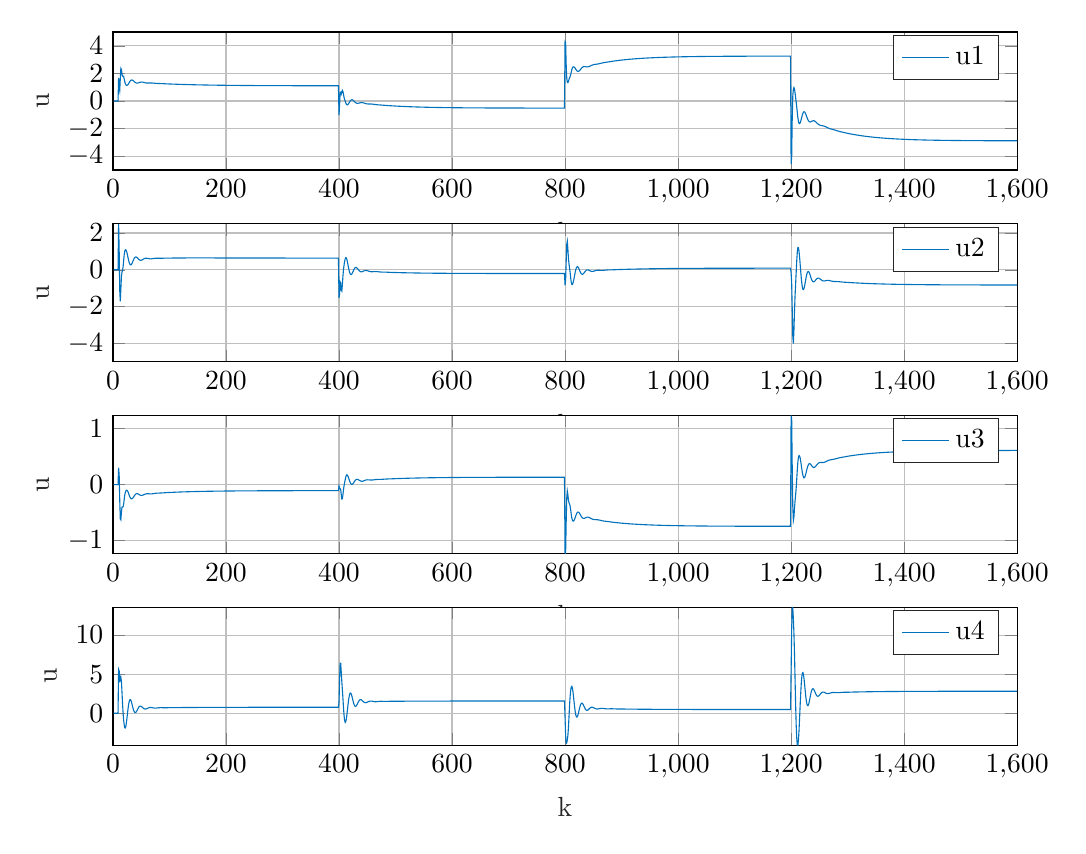
\begin{tikzpicture}

\begin{axis}[%
width=4.521in,
height=0.69in,
at={(0.758in,3.357in)},
scale only axis,
xmin=0,
xmax=1600,
xlabel style={font=\color{white!15!black}},
xlabel={k},
ymin=-5,
ymax=5,
ylabel style={font=\color{white!15!black}},
ylabel={u},
axis background/.style={fill=white},
xmajorgrids,
ymajorgrids,
legend style={legend cell align=left, align=left, draw=white!15!black}
]
\addplot [color=mycolor1]
  table[row sep=crcr]{%
1	0\\
2	0\\
3	0\\
4	0\\
5	0\\
6	0\\
7	0\\
8	0\\
9	0\\
10	1.6799\\
11	0.9612\\
12	0.74144\\
13	1.6514\\
14	2.3624\\
15	2.2903\\
16	1.9453\\
17	1.8025\\
18	1.8144\\
19	1.7598\\
20	1.5857\\
21	1.3865\\
22	1.2445\\
23	1.1697\\
24	1.1387\\
25	1.1363\\
26	1.1609\\
27	1.2113\\
28	1.2792\\
29	1.3523\\
30	1.419\\
31	1.4719\\
32	1.5067\\
33	1.5221\\
34	1.5191\\
35	1.5002\\
36	1.4697\\
37	1.4327\\
38	1.3943\\
39	1.359\\
40	1.3302\\
41	1.3101\\
42	1.2994\\
43	1.2977\\
44	1.3036\\
45	1.3149\\
46	1.3292\\
47	1.344\\
48	1.3572\\
49	1.3672\\
50	1.373\\
51	1.3743\\
52	1.3711\\
53	1.3644\\
54	1.3551\\
55	1.3444\\
56	1.3335\\
57	1.3234\\
58	1.3149\\
59	1.3085\\
60	1.3042\\
61	1.302\\
62	1.3016\\
63	1.3024\\
64	1.3038\\
65	1.3054\\
66	1.3065\\
67	1.307\\
68	1.3064\\
69	1.3048\\
70	1.3022\\
71	1.2989\\
72	1.295\\
73	1.2908\\
74	1.2866\\
75	1.2827\\
76	1.2791\\
77	1.2761\\
78	1.2735\\
79	1.2715\\
80	1.2699\\
81	1.2686\\
82	1.2674\\
83	1.2663\\
84	1.2651\\
85	1.2637\\
86	1.2622\\
87	1.2604\\
88	1.2583\\
89	1.2562\\
90	1.2539\\
91	1.2516\\
92	1.2493\\
93	1.2471\\
94	1.2449\\
95	1.243\\
96	1.2411\\
97	1.2394\\
98	1.2378\\
99	1.2363\\
100	1.2348\\
101	1.2334\\
102	1.2319\\
103	1.2304\\
104	1.2289\\
105	1.2273\\
106	1.2257\\
107	1.2241\\
108	1.2225\\
109	1.2209\\
110	1.2192\\
111	1.2177\\
112	1.2161\\
113	1.2147\\
114	1.2132\\
115	1.2118\\
116	1.2104\\
117	1.2091\\
118	1.2078\\
119	1.2065\\
120	1.2052\\
121	1.2039\\
122	1.2026\\
123	1.2013\\
124	1.2001\\
125	1.1988\\
126	1.1975\\
127	1.1963\\
128	1.195\\
129	1.1938\\
130	1.1926\\
131	1.1915\\
132	1.1903\\
133	1.1892\\
134	1.188\\
135	1.1869\\
136	1.1859\\
137	1.1848\\
138	1.1837\\
139	1.1827\\
140	1.1816\\
141	1.1806\\
142	1.1796\\
143	1.1786\\
144	1.1776\\
145	1.1766\\
146	1.1756\\
147	1.1746\\
148	1.1737\\
149	1.1728\\
150	1.1718\\
151	1.1709\\
152	1.17\\
153	1.1691\\
154	1.1683\\
155	1.1674\\
156	1.1666\\
157	1.1657\\
158	1.1649\\
159	1.164\\
160	1.1632\\
161	1.1624\\
162	1.1616\\
163	1.1609\\
164	1.1601\\
165	1.1593\\
166	1.1586\\
167	1.1578\\
168	1.1571\\
169	1.1563\\
170	1.1556\\
171	1.1549\\
172	1.1542\\
173	1.1535\\
174	1.1529\\
175	1.1522\\
176	1.1515\\
177	1.1509\\
178	1.1502\\
179	1.1496\\
180	1.149\\
181	1.1483\\
182	1.1477\\
183	1.1471\\
184	1.1465\\
185	1.1459\\
186	1.1453\\
187	1.1448\\
188	1.1442\\
189	1.1436\\
190	1.1431\\
191	1.1425\\
192	1.142\\
193	1.1415\\
194	1.1409\\
195	1.1404\\
196	1.1399\\
197	1.1394\\
198	1.1389\\
199	1.1384\\
200	1.1379\\
201	1.1375\\
202	1.137\\
203	1.1365\\
204	1.1361\\
205	1.1356\\
206	1.1352\\
207	1.1347\\
208	1.1343\\
209	1.1339\\
210	1.1334\\
211	1.133\\
212	1.1326\\
213	1.1322\\
214	1.1318\\
215	1.1314\\
216	1.131\\
217	1.1306\\
218	1.1302\\
219	1.1299\\
220	1.1295\\
221	1.1291\\
222	1.1288\\
223	1.1284\\
224	1.1281\\
225	1.1277\\
226	1.1274\\
227	1.127\\
228	1.1267\\
229	1.1264\\
230	1.126\\
231	1.1257\\
232	1.1254\\
233	1.1251\\
234	1.1248\\
235	1.1245\\
236	1.1242\\
237	1.1239\\
238	1.1236\\
239	1.1233\\
240	1.123\\
241	1.1228\\
242	1.1225\\
243	1.1222\\
244	1.122\\
245	1.1217\\
246	1.1214\\
247	1.1212\\
248	1.1209\\
249	1.1207\\
250	1.1204\\
251	1.1202\\
252	1.1199\\
253	1.1197\\
254	1.1195\\
255	1.1193\\
256	1.119\\
257	1.1188\\
258	1.1186\\
259	1.1184\\
260	1.1182\\
261	1.1179\\
262	1.1177\\
263	1.1175\\
264	1.1173\\
265	1.1171\\
266	1.1169\\
267	1.1167\\
268	1.1166\\
269	1.1164\\
270	1.1162\\
271	1.116\\
272	1.1158\\
273	1.1156\\
274	1.1155\\
275	1.1153\\
276	1.1151\\
277	1.115\\
278	1.1148\\
279	1.1146\\
280	1.1145\\
281	1.1143\\
282	1.1142\\
283	1.114\\
284	1.1139\\
285	1.1137\\
286	1.1136\\
287	1.1134\\
288	1.1133\\
289	1.1131\\
290	1.113\\
291	1.1129\\
292	1.1127\\
293	1.1126\\
294	1.1125\\
295	1.1123\\
296	1.1122\\
297	1.1121\\
298	1.112\\
299	1.1118\\
300	1.1117\\
301	1.1116\\
302	1.1115\\
303	1.1114\\
304	1.1113\\
305	1.1112\\
306	1.1111\\
307	1.1109\\
308	1.1108\\
309	1.1107\\
310	1.1106\\
311	1.1105\\
312	1.1104\\
313	1.1103\\
314	1.1102\\
315	1.1102\\
316	1.1101\\
317	1.11\\
318	1.1099\\
319	1.1098\\
320	1.1097\\
321	1.1096\\
322	1.1095\\
323	1.1095\\
324	1.1094\\
325	1.1093\\
326	1.1092\\
327	1.1091\\
328	1.1091\\
329	1.109\\
330	1.1089\\
331	1.1089\\
332	1.1088\\
333	1.1087\\
334	1.1086\\
335	1.1086\\
336	1.1085\\
337	1.1085\\
338	1.1084\\
339	1.1083\\
340	1.1083\\
341	1.1082\\
342	1.1082\\
343	1.1081\\
344	1.1081\\
345	1.108\\
346	1.1079\\
347	1.1079\\
348	1.1078\\
349	1.1078\\
350	1.1078\\
351	1.1077\\
352	1.1077\\
353	1.1076\\
354	1.1076\\
355	1.1075\\
356	1.1075\\
357	1.1074\\
358	1.1074\\
359	1.1074\\
360	1.1073\\
361	1.1072\\
362	1.1071\\
363	1.1071\\
364	1.107\\
365	1.1069\\
366	1.1069\\
367	1.1068\\
368	1.1068\\
369	1.1067\\
370	1.1067\\
371	1.1067\\
372	1.1066\\
373	1.1066\\
374	1.1066\\
375	1.1066\\
376	1.1066\\
377	1.1066\\
378	1.1065\\
379	1.1065\\
380	1.1064\\
381	1.1064\\
382	1.1063\\
383	1.1063\\
384	1.1062\\
385	1.1062\\
386	1.1061\\
387	1.1061\\
388	1.1061\\
389	1.106\\
390	1.106\\
391	1.106\\
392	1.106\\
393	1.106\\
394	1.1059\\
395	1.1059\\
396	1.1059\\
397	1.1059\\
398	1.1058\\
399	1.1058\\
400	-1.025\\
401	-0.31757\\
402	0.60827\\
403	0.64544\\
404	0.50233\\
405	0.62861\\
406	0.77463\\
407	0.6972\\
408	0.47082\\
409	0.25776\\
410	0.10542\\
411	-0.020498\\
412	-0.13879\\
413	-0.23183\\
414	-0.27889\\
415	-0.27823\\
416	-0.24223\\
417	-0.18513\\
418	-0.11802\\
419	-0.049917\\
420	0.010852\\
421	0.057251\\
422	0.084793\\
423	0.092133\\
424	0.080759\\
425	0.054217\\
426	0.01727\\
427	-0.024844\\
428	-0.067062\\
429	-0.10505\\
430	-0.13558\\
431	-0.15683\\
432	-0.16831\\
433	-0.17079\\
434	-0.16596\\
435	-0.15614\\
436	-0.14388\\
437	-0.13161\\
438	-0.12142\\
439	-0.11482\\
440	-0.11267\\
441	-0.11516\\
442	-0.1219\\
443	-0.13205\\
444	-0.1445\\
445	-0.158\\
446	-0.1714\\
447	-0.18369\\
448	-0.19416\\
449	-0.20241\\
450	-0.20836\\
451	-0.2122\\
452	-0.21435\\
453	-0.21535\\
454	-0.21579\\
455	-0.21623\\
456	-0.21714\\
457	-0.21886\\
458	-0.22158\\
459	-0.22531\\
460	-0.22998\\
461	-0.23536\\
462	-0.2412\\
463	-0.24722\\
464	-0.25314\\
465	-0.25875\\
466	-0.26388\\
467	-0.26845\\
468	-0.27245\\
469	-0.27592\\
470	-0.27898\\
471	-0.28174\\
472	-0.28435\\
473	-0.28693\\
474	-0.28959\\
475	-0.29241\\
476	-0.29542\\
477	-0.29864\\
478	-0.30203\\
479	-0.30555\\
480	-0.30914\\
481	-0.31273\\
482	-0.31626\\
483	-0.31968\\
484	-0.32295\\
485	-0.32607\\
486	-0.32902\\
487	-0.33182\\
488	-0.33449\\
489	-0.33708\\
490	-0.3396\\
491	-0.34208\\
492	-0.34456\\
493	-0.34705\\
494	-0.34956\\
495	-0.35209\\
496	-0.35463\\
497	-0.35718\\
498	-0.35971\\
499	-0.36222\\
500	-0.36468\\
501	-0.3671\\
502	-0.36945\\
503	-0.37175\\
504	-0.37398\\
505	-0.37615\\
506	-0.37828\\
507	-0.38036\\
508	-0.3824\\
509	-0.38441\\
510	-0.38641\\
511	-0.38838\\
512	-0.39033\\
513	-0.39227\\
514	-0.3942\\
515	-0.3961\\
516	-0.39798\\
517	-0.39983\\
518	-0.40165\\
519	-0.40344\\
520	-0.4052\\
521	-0.40693\\
522	-0.40862\\
523	-0.41028\\
524	-0.41192\\
525	-0.41352\\
526	-0.4151\\
527	-0.41666\\
528	-0.41819\\
529	-0.41971\\
530	-0.4212\\
531	-0.42267\\
532	-0.42412\\
533	-0.42556\\
534	-0.42697\\
535	-0.42836\\
536	-0.42973\\
537	-0.43108\\
538	-0.4324\\
539	-0.4337\\
540	-0.43498\\
541	-0.43624\\
542	-0.43748\\
543	-0.4387\\
544	-0.4399\\
545	-0.44109\\
546	-0.44225\\
547	-0.4434\\
548	-0.44453\\
549	-0.44564\\
550	-0.44673\\
551	-0.44781\\
552	-0.44887\\
553	-0.44992\\
554	-0.45095\\
555	-0.45196\\
556	-0.45296\\
557	-0.45394\\
558	-0.45491\\
559	-0.45586\\
560	-0.45679\\
561	-0.45771\\
562	-0.45862\\
563	-0.45951\\
564	-0.46038\\
565	-0.46125\\
566	-0.4621\\
567	-0.46293\\
568	-0.46375\\
569	-0.46456\\
570	-0.46536\\
571	-0.46615\\
572	-0.46692\\
573	-0.46768\\
574	-0.46843\\
575	-0.46916\\
576	-0.46989\\
577	-0.4706\\
578	-0.4713\\
579	-0.47199\\
580	-0.47267\\
581	-0.47334\\
582	-0.474\\
583	-0.47464\\
584	-0.47528\\
585	-0.4759\\
586	-0.47652\\
587	-0.47713\\
588	-0.47772\\
589	-0.47831\\
590	-0.47889\\
591	-0.47946\\
592	-0.48002\\
593	-0.48057\\
594	-0.48111\\
595	-0.48164\\
596	-0.48216\\
597	-0.48268\\
598	-0.48319\\
599	-0.48369\\
600	-0.48418\\
601	-0.48466\\
602	-0.48514\\
603	-0.4856\\
604	-0.48606\\
605	-0.48652\\
606	-0.48696\\
607	-0.4874\\
608	-0.48783\\
609	-0.48825\\
610	-0.48867\\
611	-0.48908\\
612	-0.48948\\
613	-0.48988\\
614	-0.49027\\
615	-0.49066\\
616	-0.49103\\
617	-0.49141\\
618	-0.49177\\
619	-0.49213\\
620	-0.49249\\
621	-0.49283\\
622	-0.49318\\
623	-0.49351\\
624	-0.49384\\
625	-0.49417\\
626	-0.49449\\
627	-0.49481\\
628	-0.49512\\
629	-0.49542\\
630	-0.49572\\
631	-0.49602\\
632	-0.49631\\
633	-0.49659\\
634	-0.49687\\
635	-0.49715\\
636	-0.49742\\
637	-0.49769\\
638	-0.49795\\
639	-0.49821\\
640	-0.49846\\
641	-0.49871\\
642	-0.49896\\
643	-0.4992\\
644	-0.49944\\
645	-0.49967\\
646	-0.4999\\
647	-0.50013\\
648	-0.50035\\
649	-0.50057\\
650	-0.50079\\
651	-0.501\\
652	-0.50121\\
653	-0.50141\\
654	-0.50161\\
655	-0.50181\\
656	-0.502\\
657	-0.5022\\
658	-0.50238\\
659	-0.50257\\
660	-0.50275\\
661	-0.50293\\
662	-0.50311\\
663	-0.50328\\
664	-0.50345\\
665	-0.50362\\
666	-0.50378\\
667	-0.50395\\
668	-0.50411\\
669	-0.50426\\
670	-0.50442\\
671	-0.50457\\
672	-0.50472\\
673	-0.50486\\
674	-0.50501\\
675	-0.50515\\
676	-0.50529\\
677	-0.50543\\
678	-0.50556\\
679	-0.50569\\
680	-0.50583\\
681	-0.50595\\
682	-0.50608\\
683	-0.5062\\
684	-0.50633\\
685	-0.50645\\
686	-0.50656\\
687	-0.50668\\
688	-0.50679\\
689	-0.50691\\
690	-0.50702\\
691	-0.50713\\
692	-0.50723\\
693	-0.50734\\
694	-0.50744\\
695	-0.50754\\
696	-0.50764\\
697	-0.50774\\
698	-0.50784\\
699	-0.50793\\
700	-0.50803\\
701	-0.50812\\
702	-0.50821\\
703	-0.5083\\
704	-0.50839\\
705	-0.50847\\
706	-0.50856\\
707	-0.50864\\
708	-0.50872\\
709	-0.5088\\
710	-0.50888\\
711	-0.50896\\
712	-0.50904\\
713	-0.50911\\
714	-0.50919\\
715	-0.50926\\
716	-0.50933\\
717	-0.5094\\
718	-0.50947\\
719	-0.50954\\
720	-0.50961\\
721	-0.50967\\
722	-0.50974\\
723	-0.5098\\
724	-0.50986\\
725	-0.50993\\
726	-0.50999\\
727	-0.51005\\
728	-0.51011\\
729	-0.51017\\
730	-0.51022\\
731	-0.51028\\
732	-0.51033\\
733	-0.51039\\
734	-0.51044\\
735	-0.5105\\
736	-0.51055\\
737	-0.5106\\
738	-0.51065\\
739	-0.5107\\
740	-0.51075\\
741	-0.5108\\
742	-0.51084\\
743	-0.51089\\
744	-0.51094\\
745	-0.51098\\
746	-0.51103\\
747	-0.51107\\
748	-0.51112\\
749	-0.51116\\
750	-0.51121\\
751	-0.51123\\
752	-0.51127\\
753	-0.51134\\
754	-0.51141\\
755	-0.51147\\
756	-0.51152\\
757	-0.51158\\
758	-0.51162\\
759	-0.51166\\
760	-0.51168\\
761	-0.5117\\
762	-0.51171\\
763	-0.51171\\
764	-0.51172\\
765	-0.51172\\
766	-0.51174\\
767	-0.51176\\
768	-0.51179\\
769	-0.51182\\
770	-0.51186\\
771	-0.51191\\
772	-0.51195\\
773	-0.512\\
774	-0.51204\\
775	-0.51208\\
776	-0.51211\\
777	-0.51214\\
778	-0.51216\\
779	-0.51218\\
780	-0.51219\\
781	-0.5122\\
782	-0.51221\\
783	-0.51222\\
784	-0.51224\\
785	-0.51226\\
786	-0.51228\\
787	-0.5123\\
788	-0.51233\\
789	-0.51236\\
790	-0.51238\\
791	-0.51241\\
792	-0.51244\\
793	-0.51246\\
794	-0.51248\\
795	-0.5125\\
796	-0.51252\\
797	-0.51253\\
798	-0.51254\\
799	-0.51256\\
800	4.3065\\
801	4.2375\\
802	2.6266\\
803	1.6582\\
804	1.3564\\
805	1.3295\\
806	1.4265\\
807	1.5659\\
808	1.6801\\
809	1.7813\\
810	1.9206\\
811	2.1018\\
812	2.2764\\
813	2.3999\\
814	2.4636\\
815	2.4818\\
816	2.4682\\
817	2.4299\\
818	2.3726\\
819	2.3061\\
820	2.2421\\
821	2.1907\\
822	2.1579\\
823	2.1462\\
824	2.1549\\
825	2.1816\\
826	2.2221\\
827	2.2711\\
828	2.3231\\
829	2.373\\
830	2.4166\\
831	2.4514\\
832	2.4759\\
833	2.4903\\
834	2.496\\
835	2.4949\\
836	2.4897\\
837	2.4831\\
838	2.4774\\
839	2.4745\\
840	2.4759\\
841	2.4819\\
842	2.4926\\
843	2.5073\\
844	2.525\\
845	2.5444\\
846	2.5643\\
847	2.5834\\
848	2.6009\\
849	2.6161\\
850	2.6289\\
851	2.6392\\
852	2.6474\\
853	2.654\\
854	2.6595\\
855	2.6647\\
856	2.67\\
857	2.6759\\
858	2.6827\\
859	2.6905\\
860	2.6992\\
861	2.7087\\
862	2.7189\\
863	2.7292\\
864	2.7396\\
865	2.7496\\
866	2.7592\\
867	2.7682\\
868	2.7765\\
869	2.7841\\
870	2.7912\\
871	2.7978\\
872	2.8042\\
873	2.8103\\
874	2.8164\\
875	2.8226\\
876	2.829\\
877	2.8355\\
878	2.8421\\
879	2.8488\\
880	2.8556\\
881	2.8624\\
882	2.8691\\
883	2.8756\\
884	2.882\\
885	2.8882\\
886	2.8941\\
887	2.8999\\
888	2.9054\\
889	2.9108\\
890	2.916\\
891	2.9212\\
892	2.9263\\
893	2.9313\\
894	2.9363\\
895	2.9413\\
896	2.9463\\
897	2.9513\\
898	2.9562\\
899	2.961\\
900	2.9658\\
901	2.9705\\
902	2.9751\\
903	2.9796\\
904	2.984\\
905	2.9883\\
906	2.9925\\
907	2.9967\\
908	3.0007\\
909	3.0047\\
910	3.0087\\
911	3.0126\\
912	3.0164\\
913	3.0202\\
914	3.0239\\
915	3.0276\\
916	3.0313\\
917	3.0349\\
918	3.0384\\
919	3.0419\\
920	3.0453\\
921	3.0486\\
922	3.0519\\
923	3.0552\\
924	3.0584\\
925	3.0615\\
926	3.0646\\
927	3.0676\\
928	3.0706\\
929	3.0735\\
930	3.0764\\
931	3.0793\\
932	3.0821\\
933	3.0848\\
934	3.0876\\
935	3.0903\\
936	3.0929\\
937	3.0955\\
938	3.0981\\
939	3.1006\\
940	3.1031\\
941	3.1055\\
942	3.1079\\
943	3.1102\\
944	3.1126\\
945	3.1148\\
946	3.1171\\
947	3.1193\\
948	3.1215\\
949	3.1236\\
950	3.1257\\
951	3.1278\\
952	3.1299\\
953	3.1319\\
954	3.1339\\
955	3.1358\\
956	3.1377\\
957	3.1396\\
958	3.1415\\
959	3.1433\\
960	3.1451\\
961	3.1469\\
962	3.1486\\
963	3.1503\\
964	3.152\\
965	3.1537\\
966	3.1553\\
967	3.1569\\
968	3.1585\\
969	3.1601\\
970	3.1616\\
971	3.1631\\
972	3.1646\\
973	3.1661\\
974	3.1675\\
975	3.1689\\
976	3.1703\\
977	3.1717\\
978	3.173\\
979	3.1744\\
980	3.1757\\
981	3.1769\\
982	3.1782\\
983	3.1795\\
984	3.1807\\
985	3.1819\\
986	3.1831\\
987	3.1842\\
988	3.1854\\
989	3.1865\\
990	3.1876\\
991	3.1887\\
992	3.1898\\
993	3.1909\\
994	3.1919\\
995	3.1929\\
996	3.194\\
997	3.1949\\
998	3.1959\\
999	3.1969\\
1000	3.1978\\
1001	3.1988\\
1002	3.1997\\
1003	3.2006\\
1004	3.2015\\
1005	3.2024\\
1006	3.2032\\
1007	3.2041\\
1008	3.2049\\
1009	3.2057\\
1010	3.2065\\
1011	3.2073\\
1012	3.2081\\
1013	3.2089\\
1014	3.2096\\
1015	3.2104\\
1016	3.2111\\
1017	3.2118\\
1018	3.2125\\
1019	3.2132\\
1020	3.2139\\
1021	3.2146\\
1022	3.2152\\
1023	3.2159\\
1024	3.2165\\
1025	3.2172\\
1026	3.2178\\
1027	3.2184\\
1028	3.219\\
1029	3.2196\\
1030	3.2202\\
1031	3.2208\\
1032	3.2213\\
1033	3.2219\\
1034	3.2224\\
1035	3.223\\
1036	3.2235\\
1037	3.224\\
1038	3.2245\\
1039	3.225\\
1040	3.2255\\
1041	3.226\\
1042	3.2265\\
1043	3.227\\
1044	3.2274\\
1045	3.2279\\
1046	3.2283\\
1047	3.2288\\
1048	3.2292\\
1049	3.2296\\
1050	3.2301\\
1051	3.2305\\
1052	3.2309\\
1053	3.2313\\
1054	3.2317\\
1055	3.2321\\
1056	3.2325\\
1057	3.2328\\
1058	3.2332\\
1059	3.2336\\
1060	3.2339\\
1061	3.2343\\
1062	3.2346\\
1063	3.235\\
1064	3.2353\\
1065	3.2356\\
1066	3.236\\
1067	3.2363\\
1068	3.2366\\
1069	3.2369\\
1070	3.2372\\
1071	3.2375\\
1072	3.2378\\
1073	3.2381\\
1074	3.2384\\
1075	3.2387\\
1076	3.2389\\
1077	3.2392\\
1078	3.2395\\
1079	3.2397\\
1080	3.24\\
1081	3.2402\\
1082	3.2405\\
1083	3.2407\\
1084	3.241\\
1085	3.2412\\
1086	3.2415\\
1087	3.2417\\
1088	3.2419\\
1089	3.2421\\
1090	3.2424\\
1091	3.2426\\
1092	3.2428\\
1093	3.243\\
1094	3.2432\\
1095	3.2434\\
1096	3.2436\\
1097	3.2438\\
1098	3.244\\
1099	3.2442\\
1100	3.2444\\
1101	3.2446\\
1102	3.2447\\
1103	3.2449\\
1104	3.2451\\
1105	3.2453\\
1106	3.2454\\
1107	3.2456\\
1108	3.2458\\
1109	3.2459\\
1110	3.2461\\
1111	3.2462\\
1112	3.2464\\
1113	3.2465\\
1114	3.2467\\
1115	3.2468\\
1116	3.247\\
1117	3.2471\\
1118	3.2473\\
1119	3.2474\\
1120	3.2475\\
1121	3.2477\\
1122	3.2478\\
1123	3.2479\\
1124	3.2481\\
1125	3.2482\\
1126	3.2483\\
1127	3.2484\\
1128	3.2486\\
1129	3.2487\\
1130	3.2488\\
1131	3.2489\\
1132	3.249\\
1133	3.2491\\
1134	3.2492\\
1135	3.2493\\
1136	3.2494\\
1137	3.2496\\
1138	3.2497\\
1139	3.2498\\
1140	3.2499\\
1141	3.25\\
1142	3.2501\\
1143	3.2501\\
1144	3.2502\\
1145	3.2503\\
1146	3.2504\\
1147	3.2505\\
1148	3.2506\\
1149	3.2507\\
1150	3.2508\\
1151	3.2509\\
1152	3.2509\\
1153	3.2511\\
1154	3.2512\\
1155	3.2513\\
1156	3.2514\\
1157	3.2515\\
1158	3.2515\\
1159	3.2516\\
1160	3.2517\\
1161	3.2517\\
1162	3.2518\\
1163	3.2518\\
1164	3.2518\\
1165	3.2519\\
1166	3.2519\\
1167	3.252\\
1168	3.252\\
1169	3.2521\\
1170	3.2521\\
1171	3.2522\\
1172	3.2523\\
1173	3.2524\\
1174	3.2525\\
1175	3.2525\\
1176	3.2526\\
1177	3.2526\\
1178	3.2527\\
1179	3.2527\\
1180	3.2528\\
1181	3.2528\\
1182	3.2528\\
1183	3.2529\\
1184	3.2529\\
1185	3.253\\
1186	3.253\\
1187	3.253\\
1188	3.2531\\
1189	3.2531\\
1190	3.2532\\
1191	3.2532\\
1192	3.2533\\
1193	3.2533\\
1194	3.2534\\
1195	3.2534\\
1196	3.2534\\
1197	3.2535\\
1198	3.2535\\
1199	3.2535\\
1200	-4.5792\\
1201	-4.094\\
1202	-1.2073\\
1203	0.37858\\
1204	0.85976\\
1205	0.98115\\
1206	0.87792\\
1207	0.58695\\
1208	0.24845\\
1209	-0.079304\\
1210	-0.44045\\
1211	-0.84318\\
1212	-1.2154\\
1213	-1.4796\\
1214	-1.613\\
1215	-1.6377\\
1216	-1.5829\\
1217	-1.4703\\
1218	-1.319\\
1219	-1.153\\
1220	-0.99825\\
1221	-0.8761\\
1222	-0.79963\\
1223	-0.77348\\
1224	-0.79553\\
1225	-0.85866\\
1226	-0.95213\\
1227	-1.0632\\
1228	-1.1788\\
1229	-1.2871\\
1230	-1.3792\\
1231	-1.4491\\
1232	-1.4947\\
1233	-1.5167\\
1234	-1.5187\\
1235	-1.5061\\
1236	-1.4851\\
1237	-1.4619\\
1238	-1.4422\\
1239	-1.4302\\
1240	-1.4287\\
1241	-1.4386\\
1242	-1.4595\\
1243	-1.4896\\
1244	-1.5263\\
1245	-1.5665\\
1246	-1.6074\\
1247	-1.6461\\
1248	-1.6807\\
1249	-1.7099\\
1250	-1.7332\\
1251	-1.7509\\
1252	-1.7639\\
1253	-1.7734\\
1254	-1.7809\\
1255	-1.7878\\
1256	-1.7954\\
1257	-1.8047\\
1258	-1.8163\\
1259	-1.8303\\
1260	-1.8466\\
1261	-1.8649\\
1262	-1.8844\\
1263	-1.9045\\
1264	-1.9246\\
1265	-1.9439\\
1266	-1.962\\
1267	-1.9787\\
1268	-1.9939\\
1269	-2.0077\\
1270	-2.0202\\
1271	-2.0318\\
1272	-2.0428\\
1273	-2.0536\\
1274	-2.0644\\
1275	-2.0755\\
1276	-2.0869\\
1277	-2.0989\\
1278	-2.1112\\
1279	-2.1238\\
1280	-2.1365\\
1281	-2.1493\\
1282	-2.1619\\
1283	-2.1742\\
1284	-2.186\\
1285	-2.1975\\
1286	-2.2084\\
1287	-2.219\\
1288	-2.2291\\
1289	-2.2389\\
1290	-2.2485\\
1291	-2.2579\\
1292	-2.2672\\
1293	-2.2765\\
1294	-2.2858\\
1295	-2.2951\\
1296	-2.3043\\
1297	-2.3136\\
1298	-2.3227\\
1299	-2.3318\\
1300	-2.3407\\
1301	-2.3495\\
1302	-2.3581\\
1303	-2.3665\\
1304	-2.3747\\
1305	-2.3827\\
1306	-2.3905\\
1307	-2.3981\\
1308	-2.4057\\
1309	-2.4131\\
1310	-2.4204\\
1311	-2.4276\\
1312	-2.4348\\
1313	-2.4419\\
1314	-2.4488\\
1315	-2.4558\\
1316	-2.4626\\
1317	-2.4693\\
1318	-2.4759\\
1319	-2.4824\\
1320	-2.4888\\
1321	-2.4951\\
1322	-2.5013\\
1323	-2.5073\\
1324	-2.5133\\
1325	-2.5191\\
1326	-2.5249\\
1327	-2.5306\\
1328	-2.5362\\
1329	-2.5417\\
1330	-2.5471\\
1331	-2.5524\\
1332	-2.5577\\
1333	-2.5629\\
1334	-2.568\\
1335	-2.5731\\
1336	-2.578\\
1337	-2.5829\\
1338	-2.5877\\
1339	-2.5925\\
1340	-2.5971\\
1341	-2.6017\\
1342	-2.6062\\
1343	-2.6106\\
1344	-2.615\\
1345	-2.6193\\
1346	-2.6235\\
1347	-2.6277\\
1348	-2.6318\\
1349	-2.6358\\
1350	-2.6398\\
1351	-2.6437\\
1352	-2.6476\\
1353	-2.6514\\
1354	-2.6551\\
1355	-2.6588\\
1356	-2.6624\\
1357	-2.666\\
1358	-2.6695\\
1359	-2.673\\
1360	-2.6764\\
1361	-2.6797\\
1362	-2.683\\
1363	-2.6862\\
1364	-2.6894\\
1365	-2.6926\\
1366	-2.6956\\
1367	-2.6987\\
1368	-2.7017\\
1369	-2.7046\\
1370	-2.7075\\
1371	-2.7104\\
1372	-2.7132\\
1373	-2.716\\
1374	-2.7187\\
1375	-2.7214\\
1376	-2.724\\
1377	-2.7266\\
1378	-2.7292\\
1379	-2.7317\\
1380	-2.7342\\
1381	-2.7366\\
1382	-2.739\\
1383	-2.7414\\
1384	-2.7437\\
1385	-2.746\\
1386	-2.7482\\
1387	-2.7504\\
1388	-2.7526\\
1389	-2.7548\\
1390	-2.7569\\
1391	-2.759\\
1392	-2.761\\
1393	-2.763\\
1394	-2.765\\
1395	-2.767\\
1396	-2.7689\\
1397	-2.7708\\
1398	-2.7726\\
1399	-2.7744\\
1400	-2.7763\\
1401	-2.778\\
1402	-2.7798\\
1403	-2.7815\\
1404	-2.7832\\
1405	-2.7848\\
1406	-2.7865\\
1407	-2.7881\\
1408	-2.7897\\
1409	-2.7912\\
1410	-2.7928\\
1411	-2.7943\\
1412	-2.7958\\
1413	-2.7972\\
1414	-2.7987\\
1415	-2.8001\\
1416	-2.8015\\
1417	-2.8028\\
1418	-2.8042\\
1419	-2.8055\\
1420	-2.8068\\
1421	-2.8081\\
1422	-2.8094\\
1423	-2.8106\\
1424	-2.8118\\
1425	-2.8131\\
1426	-2.8142\\
1427	-2.8154\\
1428	-2.8166\\
1429	-2.8177\\
1430	-2.8188\\
1431	-2.8199\\
1432	-2.821\\
1433	-2.822\\
1434	-2.8231\\
1435	-2.8241\\
1436	-2.8251\\
1437	-2.8261\\
1438	-2.8271\\
1439	-2.828\\
1440	-2.829\\
1441	-2.8299\\
1442	-2.8308\\
1443	-2.8317\\
1444	-2.8326\\
1445	-2.8335\\
1446	-2.8344\\
1447	-2.8352\\
1448	-2.836\\
1449	-2.8369\\
1450	-2.8377\\
1451	-2.8385\\
1452	-2.8392\\
1453	-2.84\\
1454	-2.8408\\
1455	-2.8415\\
1456	-2.8422\\
1457	-2.8429\\
1458	-2.8437\\
1459	-2.8444\\
1460	-2.845\\
1461	-2.8457\\
1462	-2.8464\\
1463	-2.847\\
1464	-2.8477\\
1465	-2.8483\\
1466	-2.8489\\
1467	-2.8495\\
1468	-2.8501\\
1469	-2.8507\\
1470	-2.8513\\
1471	-2.8519\\
1472	-2.8524\\
1473	-2.853\\
1474	-2.8535\\
1475	-2.8541\\
1476	-2.8546\\
1477	-2.8551\\
1478	-2.8556\\
1479	-2.8561\\
1480	-2.8566\\
1481	-2.8571\\
1482	-2.8576\\
1483	-2.8581\\
1484	-2.8585\\
1485	-2.859\\
1486	-2.8594\\
1487	-2.8599\\
1488	-2.8603\\
1489	-2.8607\\
1490	-2.8612\\
1491	-2.8616\\
1492	-2.862\\
1493	-2.8624\\
1494	-2.8628\\
1495	-2.8632\\
1496	-2.8635\\
1497	-2.8639\\
1498	-2.8643\\
1499	-2.8646\\
1500	-2.865\\
1501	-2.8654\\
1502	-2.8657\\
1503	-2.866\\
1504	-2.8664\\
1505	-2.8667\\
1506	-2.867\\
1507	-2.8674\\
1508	-2.8677\\
1509	-2.868\\
1510	-2.8683\\
1511	-2.8686\\
1512	-2.8689\\
1513	-2.8692\\
1514	-2.8694\\
1515	-2.8697\\
1516	-2.87\\
1517	-2.8703\\
1518	-2.8705\\
1519	-2.8708\\
1520	-2.8711\\
1521	-2.8713\\
1522	-2.8716\\
1523	-2.8718\\
1524	-2.8721\\
1525	-2.8723\\
1526	-2.8725\\
1527	-2.8728\\
1528	-2.873\\
1529	-2.8732\\
1530	-2.8734\\
1531	-2.8736\\
1532	-2.8739\\
1533	-2.8741\\
1534	-2.8743\\
1535	-2.8745\\
1536	-2.8747\\
1537	-2.8749\\
1538	-2.8751\\
1539	-2.8753\\
1540	-2.8754\\
1541	-2.8756\\
1542	-2.8758\\
1543	-2.876\\
1544	-2.8762\\
1545	-2.8763\\
1546	-2.8765\\
1547	-2.8767\\
1548	-2.8769\\
1549	-2.877\\
1550	-2.8772\\
1551	-2.8773\\
1552	-2.8775\\
1553	-2.8777\\
1554	-2.8779\\
1555	-2.8782\\
1556	-2.8784\\
1557	-2.8785\\
1558	-2.8787\\
1559	-2.8788\\
1560	-2.879\\
1561	-2.879\\
1562	-2.8791\\
1563	-2.8792\\
1564	-2.8792\\
1565	-2.8793\\
1566	-2.8794\\
1567	-2.8794\\
1568	-2.8796\\
1569	-2.8797\\
1570	-2.8798\\
1571	-2.88\\
1572	-2.8801\\
1573	-2.8803\\
1574	-2.8804\\
1575	-2.8806\\
1576	-2.8807\\
1577	-2.8808\\
1578	-2.8809\\
1579	-2.881\\
1580	-2.881\\
1581	-2.8811\\
1582	-2.8812\\
1583	-2.8812\\
1584	-2.8813\\
1585	-2.8814\\
1586	-2.8815\\
1587	-2.8815\\
1588	-2.8816\\
1589	-2.8817\\
1590	-2.8818\\
1591	-2.8819\\
1592	-2.882\\
1593	-2.8821\\
1594	-2.8822\\
1595	-2.8823\\
1596	-2.8823\\
1597	-2.8824\\
1598	-2.8825\\
1599	-2.8825\\
1600	-2.8826\\
};
\addlegendentry{u1}

\end{axis}

\begin{axis}[%
width=4.521in,
height=0.69in,
at={(0.758in,2.398in)},
scale only axis,
xmin=0,
xmax=1600,
xlabel style={font=\color{white!15!black}},
xlabel={k},
ymin=-5,
ymax=2.4974,
ylabel style={font=\color{white!15!black}},
ylabel={u},
axis background/.style={fill=white},
xmajorgrids,
ymajorgrids,
legend style={legend cell align=left, align=left, draw=white!15!black}
]
\addplot [color=mycolor1]
  table[row sep=crcr]{%
1	0\\
2	0\\
3	0\\
4	0\\
5	0\\
6	0\\
7	0\\
8	0\\
9	0\\
10	2.4974\\
11	1.0825\\
12	-1.1248\\
13	-1.7098\\
14	-1.0425\\
15	-0.36821\\
16	-0.1265\\
17	-0.034109\\
18	0.1889\\
19	0.52872\\
20	0.83687\\
21	1.0234\\
22	1.091\\
23	1.0769\\
24	1.0083\\
25	0.89877\\
26	0.76082\\
27	0.61286\\
28	0.47572\\
29	0.36643\\
30	0.29477\\
31	0.26346\\
32	0.26988\\
33	0.30775\\
34	0.36834\\
35	0.4415\\
36	0.51697\\
37	0.58568\\
38	0.64073\\
39	0.67793\\
40	0.69583\\
41	0.69549\\
42	0.67996\\
43	0.6536\\
44	0.62141\\
45	0.58834\\
46	0.55866\\
47	0.53564\\
48	0.52122\\
49	0.51604\\
50	0.51956\\
51	0.53027\\
52	0.54603\\
53	0.56444\\
54	0.58312\\
55	0.60002\\
56	0.61362\\
57	0.623\\
58	0.62787\\
59	0.62853\\
60	0.62572\\
61	0.62047\\
62	0.61394\\
63	0.60728\\
64	0.60146\\
65	0.59721\\
66	0.59494\\
67	0.59478\\
68	0.59658\\
69	0.59998\\
70	0.60447\\
71	0.6095\\
72	0.61451\\
73	0.61904\\
74	0.62276\\
75	0.62546\\
76	0.6271\\
77	0.62776\\
78	0.6276\\
79	0.62689\\
80	0.62589\\
81	0.62486\\
82	0.62403\\
83	0.62355\\
84	0.62352\\
85	0.62396\\
86	0.62484\\
87	0.62606\\
88	0.6275\\
89	0.62904\\
90	0.63056\\
91	0.63194\\
92	0.63311\\
93	0.63403\\
94	0.63469\\
95	0.63512\\
96	0.63535\\
97	0.63544\\
98	0.63547\\
99	0.63548\\
100	0.63553\\
101	0.63566\\
102	0.63588\\
103	0.6362\\
104	0.63661\\
105	0.63709\\
106	0.63761\\
107	0.63814\\
108	0.63866\\
109	0.63913\\
110	0.63955\\
111	0.6399\\
112	0.64018\\
113	0.6404\\
114	0.64058\\
115	0.64071\\
116	0.64082\\
117	0.64093\\
118	0.64104\\
119	0.64116\\
120	0.6413\\
121	0.64146\\
122	0.64163\\
123	0.64182\\
124	0.642\\
125	0.64219\\
126	0.64236\\
127	0.64252\\
128	0.64266\\
129	0.64279\\
130	0.64289\\
131	0.64298\\
132	0.64305\\
133	0.64311\\
134	0.64316\\
135	0.64321\\
136	0.64325\\
137	0.64329\\
138	0.64334\\
139	0.64339\\
140	0.64343\\
141	0.64348\\
142	0.64353\\
143	0.64357\\
144	0.6436\\
145	0.64364\\
146	0.64366\\
147	0.64368\\
148	0.64369\\
149	0.6437\\
150	0.6437\\
151	0.6437\\
152	0.64369\\
153	0.64368\\
154	0.64367\\
155	0.64365\\
156	0.64364\\
157	0.64362\\
158	0.64361\\
159	0.64359\\
160	0.64357\\
161	0.64355\\
162	0.64352\\
163	0.6435\\
164	0.64347\\
165	0.64344\\
166	0.64341\\
167	0.64337\\
168	0.64333\\
169	0.6433\\
170	0.64326\\
171	0.64321\\
172	0.64317\\
173	0.64312\\
174	0.64308\\
175	0.64303\\
176	0.64298\\
177	0.64294\\
178	0.64289\\
179	0.64284\\
180	0.64279\\
181	0.64274\\
182	0.64269\\
183	0.64263\\
184	0.64258\\
185	0.64253\\
186	0.64247\\
187	0.64242\\
188	0.64236\\
189	0.64231\\
190	0.64225\\
191	0.64219\\
192	0.64214\\
193	0.64208\\
194	0.64202\\
195	0.64196\\
196	0.6419\\
197	0.64185\\
198	0.64179\\
199	0.64173\\
200	0.64167\\
201	0.64161\\
202	0.64155\\
203	0.64149\\
204	0.64144\\
205	0.64138\\
206	0.64132\\
207	0.64126\\
208	0.6412\\
209	0.64114\\
210	0.64108\\
211	0.64102\\
212	0.64097\\
213	0.64091\\
214	0.64085\\
215	0.64079\\
216	0.64074\\
217	0.64068\\
218	0.64062\\
219	0.64056\\
220	0.64051\\
221	0.64045\\
222	0.64039\\
223	0.64034\\
224	0.64028\\
225	0.64023\\
226	0.64017\\
227	0.64012\\
228	0.64006\\
229	0.64001\\
230	0.63996\\
231	0.6399\\
232	0.63985\\
233	0.6398\\
234	0.63974\\
235	0.63969\\
236	0.63964\\
237	0.63959\\
238	0.63954\\
239	0.63949\\
240	0.63944\\
241	0.63939\\
242	0.63934\\
243	0.63929\\
244	0.63924\\
245	0.63919\\
246	0.63914\\
247	0.6391\\
248	0.63905\\
249	0.639\\
250	0.63896\\
251	0.63891\\
252	0.63886\\
253	0.63882\\
254	0.63877\\
255	0.63873\\
256	0.63869\\
257	0.63864\\
258	0.6386\\
259	0.63856\\
260	0.63851\\
261	0.63847\\
262	0.63843\\
263	0.63839\\
264	0.63835\\
265	0.63831\\
266	0.63827\\
267	0.63823\\
268	0.63819\\
269	0.63815\\
270	0.63811\\
271	0.63807\\
272	0.63804\\
273	0.638\\
274	0.63796\\
275	0.63792\\
276	0.63789\\
277	0.63785\\
278	0.63782\\
279	0.63778\\
280	0.63775\\
281	0.63771\\
282	0.63768\\
283	0.63765\\
284	0.63761\\
285	0.63758\\
286	0.63755\\
287	0.63751\\
288	0.63748\\
289	0.63745\\
290	0.63742\\
291	0.63739\\
292	0.63736\\
293	0.63733\\
294	0.6373\\
295	0.63727\\
296	0.63724\\
297	0.63721\\
298	0.63718\\
299	0.63715\\
300	0.63713\\
301	0.6371\\
302	0.63707\\
303	0.63705\\
304	0.63702\\
305	0.63699\\
306	0.63697\\
307	0.63694\\
308	0.63692\\
309	0.63689\\
310	0.63687\\
311	0.63684\\
312	0.63682\\
313	0.63679\\
314	0.63677\\
315	0.63675\\
316	0.63672\\
317	0.6367\\
318	0.63668\\
319	0.63666\\
320	0.63663\\
321	0.63661\\
322	0.63659\\
323	0.63657\\
324	0.63655\\
325	0.63653\\
326	0.63651\\
327	0.63649\\
328	0.63647\\
329	0.63645\\
330	0.63643\\
331	0.63641\\
332	0.63639\\
333	0.63638\\
334	0.63636\\
335	0.63634\\
336	0.63632\\
337	0.63631\\
338	0.63629\\
339	0.63627\\
340	0.63626\\
341	0.63624\\
342	0.63622\\
343	0.63621\\
344	0.63619\\
345	0.63618\\
346	0.63616\\
347	0.63615\\
348	0.63614\\
349	0.63612\\
350	0.63611\\
351	0.63609\\
352	0.63608\\
353	0.63607\\
354	0.63605\\
355	0.63604\\
356	0.63603\\
357	0.63601\\
358	0.636\\
359	0.63599\\
360	0.63598\\
361	0.63598\\
362	0.636\\
363	0.63602\\
364	0.63603\\
365	0.63603\\
366	0.63604\\
367	0.63603\\
368	0.63602\\
369	0.63598\\
370	0.63594\\
371	0.63589\\
372	0.63584\\
373	0.63579\\
374	0.63576\\
375	0.63573\\
376	0.63571\\
377	0.63571\\
378	0.63572\\
379	0.63574\\
380	0.63576\\
381	0.63578\\
382	0.6358\\
383	0.63582\\
384	0.63582\\
385	0.63582\\
386	0.6358\\
387	0.63578\\
388	0.63576\\
389	0.63573\\
390	0.6357\\
391	0.63567\\
392	0.63565\\
393	0.63563\\
394	0.63562\\
395	0.63562\\
396	0.63562\\
397	0.63562\\
398	0.63563\\
399	0.63563\\
400	-1.5208\\
401	-1.3371\\
402	-0.65635\\
403	-0.71357\\
404	-1.1095\\
405	-1.1578\\
406	-0.79323\\
407	-0.32895\\
408	0.025873\\
409	0.26885\\
410	0.45558\\
411	0.59528\\
412	0.66278\\
413	0.64387\\
414	0.55089\\
415	0.41079\\
416	0.25067\\
417	0.09217\\
418	-0.048149\\
419	-0.15786\\
420	-0.22908\\
421	-0.2593\\
422	-0.25142\\
423	-0.21271\\
424	-0.15307\\
425	-0.083313\\
426	-0.013745\\
427	0.046952\\
428	0.092436\\
429	0.11911\\
430	0.12617\\
431	0.11525\\
432	0.089919\\
433	0.054911\\
434	0.015405\\
435	-0.023655\\
436	-0.058113\\
437	-0.08497\\
438	-0.10257\\
439	-0.11059\\
440	-0.10989\\
441	-0.10222\\
442	-0.089866\\
443	-0.075343\\
444	-0.061021\\
445	-0.048882\\
446	-0.040345\\
447	-0.036182\\
448	-0.036522\\
449	-0.040935\\
450	-0.048567\\
451	-0.058305\\
452	-0.068949\\
453	-0.079366\\
454	-0.088616\\
455	-0.096033\\
456	-0.10126\\
457	-0.10426\\
458	-0.10525\\
459	-0.10464\\
460	-0.10299\\
461	-0.10087\\
462	-0.098816\\
463	-0.09729\\
464	-0.096603\\
465	-0.096918\\
466	-0.098253\\
467	-0.1005\\
468	-0.10345\\
469	-0.10684\\
470	-0.1104\\
471	-0.11386\\
472	-0.11702\\
473	-0.11972\\
474	-0.12189\\
475	-0.12354\\
476	-0.1247\\
477	-0.1255\\
478	-0.12604\\
479	-0.12647\\
480	-0.12692\\
481	-0.12748\\
482	-0.12822\\
483	-0.12918\\
484	-0.13036\\
485	-0.13173\\
486	-0.13325\\
487	-0.13485\\
488	-0.13647\\
489	-0.13804\\
490	-0.13953\\
491	-0.14089\\
492	-0.14212\\
493	-0.14322\\
494	-0.14419\\
495	-0.14507\\
496	-0.14588\\
497	-0.14665\\
498	-0.14742\\
499	-0.14821\\
500	-0.14902\\
501	-0.14988\\
502	-0.15078\\
503	-0.15171\\
504	-0.15266\\
505	-0.15362\\
506	-0.15457\\
507	-0.1555\\
508	-0.1564\\
509	-0.15726\\
510	-0.15807\\
511	-0.15885\\
512	-0.1596\\
513	-0.16031\\
514	-0.16099\\
515	-0.16166\\
516	-0.16233\\
517	-0.16298\\
518	-0.16364\\
519	-0.1643\\
520	-0.16496\\
521	-0.16562\\
522	-0.16627\\
523	-0.16692\\
524	-0.16756\\
525	-0.16819\\
526	-0.1688\\
527	-0.1694\\
528	-0.16998\\
529	-0.17055\\
530	-0.17109\\
531	-0.17163\\
532	-0.17215\\
533	-0.17267\\
534	-0.17317\\
535	-0.17367\\
536	-0.17417\\
537	-0.17465\\
538	-0.17514\\
539	-0.17561\\
540	-0.17608\\
541	-0.17654\\
542	-0.177\\
543	-0.17745\\
544	-0.17788\\
545	-0.17831\\
546	-0.17873\\
547	-0.17915\\
548	-0.17955\\
549	-0.17994\\
550	-0.18033\\
551	-0.18071\\
552	-0.18109\\
553	-0.18146\\
554	-0.18182\\
555	-0.18218\\
556	-0.18253\\
557	-0.18287\\
558	-0.18322\\
559	-0.18355\\
560	-0.18388\\
561	-0.1842\\
562	-0.18452\\
563	-0.18483\\
564	-0.18514\\
565	-0.18544\\
566	-0.18574\\
567	-0.18603\\
568	-0.18632\\
569	-0.1866\\
570	-0.18687\\
571	-0.18714\\
572	-0.18741\\
573	-0.18767\\
574	-0.18793\\
575	-0.18818\\
576	-0.18843\\
577	-0.18867\\
578	-0.18891\\
579	-0.18915\\
580	-0.18938\\
581	-0.18961\\
582	-0.18983\\
583	-0.19005\\
584	-0.19027\\
585	-0.19048\\
586	-0.19069\\
587	-0.1909\\
588	-0.1911\\
589	-0.1913\\
590	-0.19149\\
591	-0.19169\\
592	-0.19187\\
593	-0.19206\\
594	-0.19224\\
595	-0.19242\\
596	-0.1926\\
597	-0.19277\\
598	-0.19294\\
599	-0.19311\\
600	-0.19327\\
601	-0.19343\\
602	-0.19359\\
603	-0.19375\\
604	-0.1939\\
605	-0.19405\\
606	-0.1942\\
607	-0.19434\\
608	-0.19449\\
609	-0.19463\\
610	-0.19477\\
611	-0.1949\\
612	-0.19504\\
613	-0.19517\\
614	-0.1953\\
615	-0.19542\\
616	-0.19555\\
617	-0.19567\\
618	-0.19579\\
619	-0.19591\\
620	-0.19602\\
621	-0.19614\\
622	-0.19625\\
623	-0.19636\\
624	-0.19647\\
625	-0.19658\\
626	-0.19668\\
627	-0.19678\\
628	-0.19689\\
629	-0.19699\\
630	-0.19708\\
631	-0.19718\\
632	-0.19727\\
633	-0.19737\\
634	-0.19746\\
635	-0.19755\\
636	-0.19764\\
637	-0.19772\\
638	-0.19781\\
639	-0.19789\\
640	-0.19798\\
641	-0.19806\\
642	-0.19814\\
643	-0.19821\\
644	-0.19829\\
645	-0.19837\\
646	-0.19844\\
647	-0.19851\\
648	-0.19859\\
649	-0.19866\\
650	-0.19873\\
651	-0.19879\\
652	-0.19886\\
653	-0.19893\\
654	-0.19899\\
655	-0.19906\\
656	-0.19912\\
657	-0.19918\\
658	-0.19924\\
659	-0.1993\\
660	-0.19936\\
661	-0.19942\\
662	-0.19947\\
663	-0.19953\\
664	-0.19958\\
665	-0.19964\\
666	-0.19969\\
667	-0.19974\\
668	-0.19979\\
669	-0.19984\\
670	-0.19989\\
671	-0.19994\\
672	-0.19999\\
673	-0.20004\\
674	-0.20008\\
675	-0.20013\\
676	-0.20017\\
677	-0.20022\\
678	-0.20026\\
679	-0.2003\\
680	-0.20034\\
681	-0.20038\\
682	-0.20043\\
683	-0.20046\\
684	-0.2005\\
685	-0.20054\\
686	-0.20058\\
687	-0.20062\\
688	-0.20065\\
689	-0.20069\\
690	-0.20072\\
691	-0.20076\\
692	-0.20079\\
693	-0.20083\\
694	-0.20086\\
695	-0.20089\\
696	-0.20092\\
697	-0.20095\\
698	-0.20099\\
699	-0.20102\\
700	-0.20104\\
701	-0.20107\\
702	-0.2011\\
703	-0.20113\\
704	-0.20116\\
705	-0.20119\\
706	-0.20121\\
707	-0.20124\\
708	-0.20127\\
709	-0.20129\\
710	-0.20132\\
711	-0.20134\\
712	-0.20136\\
713	-0.20139\\
714	-0.20141\\
715	-0.20144\\
716	-0.20146\\
717	-0.20148\\
718	-0.2015\\
719	-0.20152\\
720	-0.20154\\
721	-0.20156\\
722	-0.20159\\
723	-0.20161\\
724	-0.20162\\
725	-0.20164\\
726	-0.20166\\
727	-0.20168\\
728	-0.2017\\
729	-0.20172\\
730	-0.20174\\
731	-0.20175\\
732	-0.20177\\
733	-0.20179\\
734	-0.2018\\
735	-0.20182\\
736	-0.20183\\
737	-0.20185\\
738	-0.20187\\
739	-0.20188\\
740	-0.2019\\
741	-0.20191\\
742	-0.20192\\
743	-0.20194\\
744	-0.20195\\
745	-0.20196\\
746	-0.20198\\
747	-0.20199\\
748	-0.202\\
749	-0.20202\\
750	-0.20203\\
751	-0.20204\\
752	-0.20205\\
753	-0.20204\\
754	-0.20203\\
755	-0.20201\\
756	-0.202\\
757	-0.202\\
758	-0.20202\\
759	-0.20204\\
760	-0.20208\\
761	-0.20212\\
762	-0.20217\\
763	-0.20221\\
764	-0.20225\\
765	-0.20228\\
766	-0.2023\\
767	-0.2023\\
768	-0.20229\\
769	-0.20228\\
770	-0.20225\\
771	-0.20223\\
772	-0.20221\\
773	-0.2022\\
774	-0.20219\\
775	-0.2022\\
776	-0.20221\\
777	-0.20223\\
778	-0.20226\\
779	-0.20229\\
780	-0.20231\\
781	-0.20234\\
782	-0.20236\\
783	-0.20238\\
784	-0.20239\\
785	-0.20239\\
786	-0.20239\\
787	-0.20238\\
788	-0.20237\\
789	-0.20237\\
790	-0.20236\\
791	-0.20236\\
792	-0.20236\\
793	-0.20237\\
794	-0.20237\\
795	-0.20238\\
796	-0.2024\\
797	-0.20241\\
798	-0.20242\\
799	-0.20244\\
800	-0.84034\\
801	-0.59329\\
802	0.43217\\
803	1.3735\\
804	1.5491\\
805	1.1186\\
806	0.6211\\
807	0.31353\\
808	0.1007\\
809	-0.15491\\
810	-0.44672\\
811	-0.68211\\
812	-0.79992\\
813	-0.80463\\
814	-0.73097\\
815	-0.60867\\
816	-0.45639\\
817	-0.29062\\
818	-0.13054\\
819	0.0049957\\
820	0.10261\\
821	0.15659\\
822	0.16807\\
823	0.14299\\
824	0.090376\\
825	0.020911\\
826	-0.054295\\
827	-0.12504\\
828	-0.18314\\
829	-0.22319\\
830	-0.24278\\
831	-0.24231\\
832	-0.2245\\
833	-0.19372\\
834	-0.15524\\
835	-0.11443\\
836	-0.076177\\
837	-0.044313\\
838	-0.021354\\
839	-0.0083872\\
840	-0.0051609\\
841	-0.010314\\
842	-0.021706\\
843	-0.036785\\
844	-0.052953\\
845	-0.06788\\
846	-0.079739\\
847	-0.087347\\
848	-0.090206\\
849	-0.088462\\
850	-0.082787\\
851	-0.074221\\
852	-0.063995\\
853	-0.053352\\
854	-0.043402\\
855	-0.035009\\
856	-0.028725\\
857	-0.02477\\
858	-0.023061\\
859	-0.023261\\
860	-0.024862\\
861	-0.027269\\
862	-0.029883\\
863	-0.032173\\
864	-0.03373\\
865	-0.034294\\
866	-0.033766\\
867	-0.032191\\
868	-0.029737\\
869	-0.026649\\
870	-0.023215\\
871	-0.019722\\
872	-0.016422\\
873	-0.01351\\
874	-0.011106\\
875	-0.0092537\\
876	-0.007928\\
877	-0.0070464\\
878	-0.0064881\\
879	-0.0061144\\
880	-0.0057873\\
881	-0.005386\\
882	-0.0048185\\
883	-0.0040283\\
884	-0.0029955\\
885	-0.0017338\\
886	-0.0002836\\
887	0.0012965\\
888	0.0029398\\
889	0.0045803\\
890	0.0061605\\
891	0.0076373\\
892	0.0089844\\
893	0.010193\\
894	0.011271\\
895	0.012239\\
896	0.013125\\
897	0.013961\\
898	0.01478\\
899	0.015608\\
900	0.016467\\
901	0.01737\\
902	0.018319\\
903	0.019311\\
904	0.020337\\
905	0.021382\\
906	0.022432\\
907	0.023471\\
908	0.024486\\
909	0.025467\\
910	0.02641\\
911	0.027312\\
912	0.028176\\
913	0.029007\\
914	0.029811\\
915	0.030596\\
916	0.03137\\
917	0.032139\\
918	0.032908\\
919	0.033679\\
920	0.034453\\
921	0.03523\\
922	0.036006\\
923	0.03678\\
924	0.037547\\
925	0.038304\\
926	0.039048\\
927	0.039777\\
928	0.04049\\
929	0.041187\\
930	0.041868\\
931	0.042535\\
932	0.04319\\
933	0.043834\\
934	0.044469\\
935	0.045096\\
936	0.045717\\
937	0.046333\\
938	0.046943\\
939	0.047548\\
940	0.048147\\
941	0.048739\\
942	0.049323\\
943	0.0499\\
944	0.050468\\
945	0.051026\\
946	0.051576\\
947	0.052116\\
948	0.052647\\
949	0.05317\\
950	0.053684\\
951	0.054191\\
952	0.054691\\
953	0.055183\\
954	0.055669\\
955	0.056149\\
956	0.056622\\
957	0.057089\\
958	0.05755\\
959	0.058005\\
960	0.058454\\
961	0.058897\\
962	0.059333\\
963	0.059764\\
964	0.060187\\
965	0.060605\\
966	0.061017\\
967	0.061422\\
968	0.061821\\
969	0.062214\\
970	0.062601\\
971	0.062983\\
972	0.063358\\
973	0.063729\\
974	0.064094\\
975	0.064453\\
976	0.064808\\
977	0.065158\\
978	0.065502\\
979	0.065842\\
980	0.066177\\
981	0.066507\\
982	0.066832\\
983	0.067153\\
984	0.067469\\
985	0.06778\\
986	0.068086\\
987	0.068388\\
988	0.068685\\
989	0.068978\\
990	0.069267\\
991	0.069551\\
992	0.069831\\
993	0.070106\\
994	0.070378\\
995	0.070646\\
996	0.070909\\
997	0.071169\\
998	0.071425\\
999	0.071678\\
1000	0.071926\\
1001	0.072171\\
1002	0.072412\\
1003	0.07265\\
1004	0.072884\\
1005	0.073114\\
1006	0.073341\\
1007	0.073565\\
1008	0.073785\\
1009	0.074002\\
1010	0.074216\\
1011	0.074426\\
1012	0.074633\\
1013	0.074837\\
1014	0.075038\\
1015	0.075236\\
1016	0.075431\\
1017	0.075623\\
1018	0.075813\\
1019	0.075999\\
1020	0.076182\\
1021	0.076363\\
1022	0.076541\\
1023	0.076716\\
1024	0.076889\\
1025	0.077059\\
1026	0.077226\\
1027	0.077391\\
1028	0.077554\\
1029	0.077713\\
1030	0.077871\\
1031	0.078026\\
1032	0.078178\\
1033	0.078329\\
1034	0.078477\\
1035	0.078623\\
1036	0.078766\\
1037	0.078908\\
1038	0.079047\\
1039	0.079184\\
1040	0.079319\\
1041	0.079452\\
1042	0.079583\\
1043	0.079711\\
1044	0.079838\\
1045	0.079963\\
1046	0.080086\\
1047	0.080207\\
1048	0.080326\\
1049	0.080444\\
1050	0.08056\\
1051	0.080673\\
1052	0.080785\\
1053	0.080896\\
1054	0.081004\\
1055	0.081111\\
1056	0.081217\\
1057	0.081321\\
1058	0.081423\\
1059	0.081523\\
1060	0.081622\\
1061	0.08172\\
1062	0.081816\\
1063	0.08191\\
1064	0.082003\\
1065	0.082095\\
1066	0.082185\\
1067	0.082274\\
1068	0.082361\\
1069	0.082447\\
1070	0.082532\\
1071	0.082615\\
1072	0.082697\\
1073	0.082778\\
1074	0.082858\\
1075	0.082936\\
1076	0.083013\\
1077	0.083089\\
1078	0.083164\\
1079	0.083238\\
1080	0.08331\\
1081	0.083382\\
1082	0.083452\\
1083	0.083521\\
1084	0.083589\\
1085	0.083656\\
1086	0.083723\\
1087	0.083788\\
1088	0.083852\\
1089	0.083915\\
1090	0.083977\\
1091	0.084038\\
1092	0.084098\\
1093	0.084157\\
1094	0.084215\\
1095	0.084273\\
1096	0.084329\\
1097	0.084385\\
1098	0.084439\\
1099	0.084493\\
1100	0.084546\\
1101	0.084599\\
1102	0.08465\\
1103	0.084701\\
1104	0.08475\\
1105	0.084799\\
1106	0.084848\\
1107	0.084895\\
1108	0.084942\\
1109	0.084988\\
1110	0.085033\\
1111	0.085078\\
1112	0.085122\\
1113	0.085165\\
1114	0.085207\\
1115	0.085249\\
1116	0.08529\\
1117	0.085331\\
1118	0.08537\\
1119	0.085409\\
1120	0.085448\\
1121	0.085486\\
1122	0.085523\\
1123	0.08556\\
1124	0.085596\\
1125	0.085631\\
1126	0.085666\\
1127	0.0857\\
1128	0.085734\\
1129	0.085767\\
1130	0.0858\\
1131	0.085832\\
1132	0.085864\\
1133	0.085895\\
1134	0.085925\\
1135	0.085955\\
1136	0.085984\\
1137	0.086013\\
1138	0.086042\\
1139	0.08607\\
1140	0.086097\\
1141	0.086124\\
1142	0.086151\\
1143	0.086177\\
1144	0.086203\\
1145	0.086228\\
1146	0.086253\\
1147	0.086278\\
1148	0.086303\\
1149	0.086327\\
1150	0.086351\\
1151	0.086368\\
1152	0.086378\\
1153	0.086379\\
1154	0.086373\\
1155	0.086367\\
1156	0.086367\\
1157	0.086377\\
1158	0.086398\\
1159	0.086431\\
1160	0.086478\\
1161	0.086533\\
1162	0.086593\\
1163	0.086652\\
1164	0.086705\\
1165	0.086748\\
1166	0.086778\\
1167	0.086794\\
1168	0.086797\\
1169	0.08679\\
1170	0.086775\\
1171	0.086758\\
1172	0.086742\\
1173	0.086731\\
1174	0.086728\\
1175	0.086735\\
1176	0.086752\\
1177	0.086778\\
1178	0.08681\\
1179	0.086847\\
1180	0.086884\\
1181	0.08692\\
1182	0.086951\\
1183	0.086977\\
1184	0.086995\\
1185	0.087007\\
1186	0.087013\\
1187	0.087014\\
1188	0.087013\\
1189	0.087011\\
1190	0.08701\\
1191	0.087011\\
1192	0.087016\\
1193	0.087024\\
1194	0.087037\\
1195	0.087052\\
1196	0.08707\\
1197	0.087089\\
1198	0.087108\\
1199	0.087127\\
1200	-0.1613\\
1201	-0.72382\\
1202	-2.1418\\
1203	-3.6203\\
1204	-4.006\\
1205	-3.2822\\
1206	-2.2425\\
1207	-1.4177\\
1208	-0.77638\\
1209	-0.1383\\
1210	0.49378\\
1211	0.97796\\
1212	1.2114\\
1213	1.1983\\
1214	1.0034\\
1215	0.69261\\
1216	0.3171\\
1217	-0.078026\\
1218	-0.4475\\
1219	-0.75098\\
1220	-0.96121\\
1221	-1.0677\\
1222	-1.075\\
1223	-0.99883\\
1224	-0.86203\\
1225	-0.6907\\
1226	-0.51112\\
1227	-0.34674\\
1228	-0.21571\\
1229	-0.12946\\
1230	-0.092301\\
1231	-0.10205\\
1232	-0.15126\\
1233	-0.22893\\
1234	-0.32231\\
1235	-0.41871\\
1236	-0.50693\\
1237	-0.57844\\
1238	-0.62793\\
1239	-0.6535\\
1240	-0.65634\\
1241	-0.64013\\
1242	-0.61027\\
1243	-0.5729\\
1244	-0.53416\\
1245	-0.49938\\
1246	-0.47261\\
1247	-0.45635\\
1248	-0.45145\\
1249	-0.45728\\
1250	-0.47202\\
1251	-0.49307\\
1252	-0.51746\\
1253	-0.54226\\
1254	-0.56493\\
1255	-0.58356\\
1256	-0.597\\
1257	-0.60486\\
1258	-0.60751\\
1259	-0.60582\\
1260	-0.60107\\
1261	-0.59471\\
1262	-0.58813\\
1263	-0.58254\\
1264	-0.57887\\
1265	-0.57763\\
1266	-0.57901\\
1267	-0.58282\\
1268	-0.58861\\
1269	-0.59579\\
1270	-0.60364\\
1271	-0.6115\\
1272	-0.6188\\
1273	-0.6251\\
1274	-0.63016\\
1275	-0.6339\\
1276	-0.63642\\
1277	-0.63794\\
1278	-0.63876\\
1279	-0.6392\\
1280	-0.63961\\
1281	-0.64024\\
1282	-0.6413\\
1283	-0.64292\\
1284	-0.64511\\
1285	-0.64783\\
1286	-0.65099\\
1287	-0.65442\\
1288	-0.65797\\
1289	-0.66149\\
1290	-0.66484\\
1291	-0.66793\\
1292	-0.67071\\
1293	-0.67316\\
1294	-0.67531\\
1295	-0.67722\\
1296	-0.67894\\
1297	-0.68057\\
1298	-0.68217\\
1299	-0.68381\\
1300	-0.68554\\
1301	-0.68737\\
1302	-0.68932\\
1303	-0.69137\\
1304	-0.6935\\
1305	-0.69567\\
1306	-0.69784\\
1307	-0.69998\\
1308	-0.70207\\
1309	-0.70407\\
1310	-0.70599\\
1311	-0.70781\\
1312	-0.70954\\
1313	-0.7112\\
1314	-0.71281\\
1315	-0.71438\\
1316	-0.71592\\
1317	-0.71746\\
1318	-0.71901\\
1319	-0.72056\\
1320	-0.72212\\
1321	-0.72369\\
1322	-0.72527\\
1323	-0.72683\\
1324	-0.72838\\
1325	-0.72991\\
1326	-0.73142\\
1327	-0.73288\\
1328	-0.73431\\
1329	-0.73571\\
1330	-0.73707\\
1331	-0.73841\\
1332	-0.73971\\
1333	-0.741\\
1334	-0.74226\\
1335	-0.74351\\
1336	-0.74475\\
1337	-0.74598\\
1338	-0.7472\\
1339	-0.74841\\
1340	-0.74961\\
1341	-0.75079\\
1342	-0.75196\\
1343	-0.75311\\
1344	-0.75425\\
1345	-0.75536\\
1346	-0.75645\\
1347	-0.75753\\
1348	-0.75859\\
1349	-0.75962\\
1350	-0.76065\\
1351	-0.76165\\
1352	-0.76264\\
1353	-0.76362\\
1354	-0.76459\\
1355	-0.76554\\
1356	-0.76648\\
1357	-0.7674\\
1358	-0.76832\\
1359	-0.76922\\
1360	-0.77011\\
1361	-0.77099\\
1362	-0.77185\\
1363	-0.7727\\
1364	-0.77354\\
1365	-0.77437\\
1366	-0.77518\\
1367	-0.77598\\
1368	-0.77677\\
1369	-0.77755\\
1370	-0.77831\\
1371	-0.77907\\
1372	-0.77981\\
1373	-0.78054\\
1374	-0.78126\\
1375	-0.78197\\
1376	-0.78267\\
1377	-0.78336\\
1378	-0.78404\\
1379	-0.78471\\
1380	-0.78537\\
1381	-0.78602\\
1382	-0.78666\\
1383	-0.78729\\
1384	-0.78791\\
1385	-0.78852\\
1386	-0.78913\\
1387	-0.78972\\
1388	-0.7903\\
1389	-0.79088\\
1390	-0.79145\\
1391	-0.792\\
1392	-0.79255\\
1393	-0.7931\\
1394	-0.79363\\
1395	-0.79416\\
1396	-0.79467\\
1397	-0.79518\\
1398	-0.79569\\
1399	-0.79618\\
1400	-0.79667\\
1401	-0.79715\\
1402	-0.79762\\
1403	-0.79809\\
1404	-0.79855\\
1405	-0.799\\
1406	-0.79944\\
1407	-0.79988\\
1408	-0.80031\\
1409	-0.80074\\
1410	-0.80115\\
1411	-0.80157\\
1412	-0.80197\\
1413	-0.80237\\
1414	-0.80276\\
1415	-0.80315\\
1416	-0.80353\\
1417	-0.80391\\
1418	-0.80428\\
1419	-0.80464\\
1420	-0.805\\
1421	-0.80535\\
1422	-0.8057\\
1423	-0.80605\\
1424	-0.80638\\
1425	-0.80671\\
1426	-0.80704\\
1427	-0.80736\\
1428	-0.80768\\
1429	-0.80799\\
1430	-0.8083\\
1431	-0.8086\\
1432	-0.8089\\
1433	-0.80919\\
1434	-0.80948\\
1435	-0.80977\\
1436	-0.81005\\
1437	-0.81032\\
1438	-0.81059\\
1439	-0.81086\\
1440	-0.81112\\
1441	-0.81138\\
1442	-0.81164\\
1443	-0.81189\\
1444	-0.81214\\
1445	-0.81238\\
1446	-0.81262\\
1447	-0.81285\\
1448	-0.81309\\
1449	-0.81332\\
1450	-0.81354\\
1451	-0.81376\\
1452	-0.81398\\
1453	-0.81419\\
1454	-0.81441\\
1455	-0.81461\\
1456	-0.81482\\
1457	-0.81502\\
1458	-0.81522\\
1459	-0.81542\\
1460	-0.81561\\
1461	-0.8158\\
1462	-0.81598\\
1463	-0.81617\\
1464	-0.81635\\
1465	-0.81653\\
1466	-0.8167\\
1467	-0.81688\\
1468	-0.81705\\
1469	-0.81721\\
1470	-0.81738\\
1471	-0.81754\\
1472	-0.8177\\
1473	-0.81786\\
1474	-0.81801\\
1475	-0.81816\\
1476	-0.81831\\
1477	-0.81846\\
1478	-0.81861\\
1479	-0.81875\\
1480	-0.81889\\
1481	-0.81903\\
1482	-0.81917\\
1483	-0.8193\\
1484	-0.81943\\
1485	-0.81956\\
1486	-0.81969\\
1487	-0.81982\\
1488	-0.81994\\
1489	-0.82006\\
1490	-0.82018\\
1491	-0.8203\\
1492	-0.82042\\
1493	-0.82053\\
1494	-0.82065\\
1495	-0.82076\\
1496	-0.82087\\
1497	-0.82098\\
1498	-0.82108\\
1499	-0.82119\\
1500	-0.82129\\
1501	-0.82139\\
1502	-0.82149\\
1503	-0.82159\\
1504	-0.82169\\
1505	-0.82178\\
1506	-0.82187\\
1507	-0.82197\\
1508	-0.82206\\
1509	-0.82215\\
1510	-0.82223\\
1511	-0.82232\\
1512	-0.82241\\
1513	-0.82249\\
1514	-0.82257\\
1515	-0.82265\\
1516	-0.82273\\
1517	-0.82281\\
1518	-0.82289\\
1519	-0.82296\\
1520	-0.82304\\
1521	-0.82311\\
1522	-0.82318\\
1523	-0.82325\\
1524	-0.82332\\
1525	-0.82339\\
1526	-0.82346\\
1527	-0.82353\\
1528	-0.82359\\
1529	-0.82366\\
1530	-0.82372\\
1531	-0.82378\\
1532	-0.82384\\
1533	-0.8239\\
1534	-0.82396\\
1535	-0.82402\\
1536	-0.82408\\
1537	-0.82413\\
1538	-0.82419\\
1539	-0.82424\\
1540	-0.82429\\
1541	-0.82435\\
1542	-0.8244\\
1543	-0.82445\\
1544	-0.8245\\
1545	-0.82455\\
1546	-0.82459\\
1547	-0.82464\\
1548	-0.82469\\
1549	-0.82474\\
1550	-0.82478\\
1551	-0.82481\\
1552	-0.82483\\
1553	-0.82482\\
1554	-0.8248\\
1555	-0.82477\\
1556	-0.82476\\
1557	-0.82478\\
1558	-0.82483\\
1559	-0.8249\\
1560	-0.825\\
1561	-0.82513\\
1562	-0.82526\\
1563	-0.82539\\
1564	-0.8255\\
1565	-0.82559\\
1566	-0.82565\\
1567	-0.82568\\
1568	-0.82567\\
1569	-0.82564\\
1570	-0.8256\\
1571	-0.82555\\
1572	-0.82551\\
1573	-0.82548\\
1574	-0.82547\\
1575	-0.82548\\
1576	-0.82552\\
1577	-0.82558\\
1578	-0.82565\\
1579	-0.82573\\
1580	-0.82581\\
1581	-0.82589\\
1582	-0.82596\\
1583	-0.82601\\
1584	-0.82604\\
1585	-0.82606\\
1586	-0.82607\\
1587	-0.82607\\
1588	-0.82606\\
1589	-0.82605\\
1590	-0.82604\\
1591	-0.82604\\
1592	-0.82605\\
1593	-0.82606\\
1594	-0.82609\\
1595	-0.82612\\
1596	-0.82616\\
1597	-0.8262\\
1598	-0.82624\\
1599	-0.82628\\
1600	-0.82631\\
};
\addlegendentry{u2}

\end{axis}

\begin{axis}[%
width=4.521in,
height=0.69in,
at={(0.758in,1.44in)},
scale only axis,
xmin=0,
xmax=1600,
xlabel style={font=\color{white!15!black}},
xlabel={k},
ymin=-1.2273,
ymax=1.2351,
ylabel style={font=\color{white!15!black}},
ylabel={u},
axis background/.style={fill=white},
xmajorgrids,
ymajorgrids,
legend style={legend cell align=left, align=left, draw=white!15!black}
]
\addplot [color=mycolor1]
  table[row sep=crcr]{%
1	0\\
2	0\\
3	0\\
4	0\\
5	0\\
6	0\\
7	0\\
8	0\\
9	0\\
10	0.30059\\
11	0.17331\\
12	-0.2756\\
13	-0.61193\\
14	-0.62863\\
15	-0.4882\\
16	-0.40156\\
17	-0.3989\\
18	-0.39597\\
19	-0.34157\\
20	-0.25614\\
21	-0.18077\\
22	-0.13352\\
23	-0.10955\\
24	-0.099988\\
25	-0.10171\\
26	-0.11489\\
27	-0.13803\\
28	-0.16679\\
29	-0.19591\\
30	-0.22118\\
31	-0.24004\\
32	-0.25127\\
33	-0.25465\\
34	-0.25078\\
35	-0.24099\\
36	-0.22715\\
37	-0.21138\\
38	-0.19573\\
39	-0.18191\\
40	-0.17113\\
41	-0.16408\\
42	-0.1609\\
43	-0.16125\\
44	-0.16443\\
45	-0.16952\\
46	-0.17548\\
47	-0.18136\\
48	-0.18634\\
49	-0.18984\\
50	-0.19155\\
51	-0.1914\\
52	-0.18958\\
53	-0.18641\\
54	-0.18237\\
55	-0.17793\\
56	-0.17357\\
57	-0.16967\\
58	-0.1665\\
59	-0.16421\\
60	-0.16283\\
61	-0.16227\\
62	-0.16236\\
63	-0.16287\\
64	-0.16359\\
65	-0.16427\\
66	-0.16475\\
67	-0.16488\\
68	-0.16461\\
69	-0.16392\\
70	-0.16286\\
71	-0.16151\\
72	-0.15998\\
73	-0.15838\\
74	-0.15681\\
75	-0.15537\\
76	-0.15412\\
77	-0.15308\\
78	-0.15226\\
79	-0.15164\\
80	-0.15117\\
81	-0.1508\\
82	-0.15048\\
83	-0.15016\\
84	-0.1498\\
85	-0.14937\\
86	-0.14884\\
87	-0.14823\\
88	-0.14754\\
89	-0.1468\\
90	-0.14602\\
91	-0.14523\\
92	-0.14446\\
93	-0.14373\\
94	-0.14305\\
95	-0.14243\\
96	-0.14186\\
97	-0.14135\\
98	-0.14087\\
99	-0.14043\\
100	-0.14\\
101	-0.13957\\
102	-0.13914\\
103	-0.1387\\
104	-0.13824\\
105	-0.13777\\
106	-0.13728\\
107	-0.13679\\
108	-0.13629\\
109	-0.1358\\
110	-0.13532\\
111	-0.13485\\
112	-0.1344\\
113	-0.13397\\
114	-0.13356\\
115	-0.13316\\
116	-0.13277\\
117	-0.1324\\
118	-0.13203\\
119	-0.13167\\
120	-0.13131\\
121	-0.13095\\
122	-0.13059\\
123	-0.13024\\
124	-0.12988\\
125	-0.12953\\
126	-0.12918\\
127	-0.12883\\
128	-0.12849\\
129	-0.12816\\
130	-0.12783\\
131	-0.12751\\
132	-0.1272\\
133	-0.1269\\
134	-0.1266\\
135	-0.12631\\
136	-0.12603\\
137	-0.12574\\
138	-0.12546\\
139	-0.12519\\
140	-0.12492\\
141	-0.12465\\
142	-0.12438\\
143	-0.12412\\
144	-0.12386\\
145	-0.1236\\
146	-0.12335\\
147	-0.12311\\
148	-0.12286\\
149	-0.12262\\
150	-0.12239\\
151	-0.12216\\
152	-0.12193\\
153	-0.12171\\
154	-0.12149\\
155	-0.12128\\
156	-0.12106\\
157	-0.12085\\
158	-0.12065\\
159	-0.12044\\
160	-0.12024\\
161	-0.12004\\
162	-0.11985\\
163	-0.11966\\
164	-0.11947\\
165	-0.11928\\
166	-0.1191\\
167	-0.11892\\
168	-0.11874\\
169	-0.11856\\
170	-0.11839\\
171	-0.11822\\
172	-0.11805\\
173	-0.11789\\
174	-0.11773\\
175	-0.11757\\
176	-0.11741\\
177	-0.11726\\
178	-0.1171\\
179	-0.11695\\
180	-0.11681\\
181	-0.11666\\
182	-0.11652\\
183	-0.11637\\
184	-0.11624\\
185	-0.1161\\
186	-0.11596\\
187	-0.11583\\
188	-0.1157\\
189	-0.11557\\
190	-0.11544\\
191	-0.11532\\
192	-0.11519\\
193	-0.11507\\
194	-0.11495\\
195	-0.11483\\
196	-0.11472\\
197	-0.1146\\
198	-0.11449\\
199	-0.11438\\
200	-0.11427\\
201	-0.11416\\
202	-0.11405\\
203	-0.11395\\
204	-0.11385\\
205	-0.11375\\
206	-0.11365\\
207	-0.11355\\
208	-0.11345\\
209	-0.11335\\
210	-0.11326\\
211	-0.11317\\
212	-0.11308\\
213	-0.11299\\
214	-0.1129\\
215	-0.11281\\
216	-0.11272\\
217	-0.11264\\
218	-0.11256\\
219	-0.11247\\
220	-0.11239\\
221	-0.11231\\
222	-0.11223\\
223	-0.11216\\
224	-0.11208\\
225	-0.112\\
226	-0.11193\\
227	-0.11186\\
228	-0.11179\\
229	-0.11171\\
230	-0.11164\\
231	-0.11158\\
232	-0.11151\\
233	-0.11144\\
234	-0.11138\\
235	-0.11131\\
236	-0.11125\\
237	-0.11118\\
238	-0.11112\\
239	-0.11106\\
240	-0.111\\
241	-0.11094\\
242	-0.11088\\
243	-0.11083\\
244	-0.11077\\
245	-0.11072\\
246	-0.11066\\
247	-0.11061\\
248	-0.11055\\
249	-0.1105\\
250	-0.11045\\
251	-0.1104\\
252	-0.11035\\
253	-0.1103\\
254	-0.11025\\
255	-0.1102\\
256	-0.11016\\
257	-0.11011\\
258	-0.11006\\
259	-0.11002\\
260	-0.10997\\
261	-0.10993\\
262	-0.10989\\
263	-0.10984\\
264	-0.1098\\
265	-0.10976\\
266	-0.10972\\
267	-0.10968\\
268	-0.10964\\
269	-0.1096\\
270	-0.10957\\
271	-0.10953\\
272	-0.10949\\
273	-0.10946\\
274	-0.10942\\
275	-0.10938\\
276	-0.10935\\
277	-0.10932\\
278	-0.10928\\
279	-0.10925\\
280	-0.10922\\
281	-0.10918\\
282	-0.10915\\
283	-0.10912\\
284	-0.10909\\
285	-0.10906\\
286	-0.10903\\
287	-0.109\\
288	-0.10897\\
289	-0.10894\\
290	-0.10892\\
291	-0.10889\\
292	-0.10886\\
293	-0.10883\\
294	-0.10881\\
295	-0.10878\\
296	-0.10876\\
297	-0.10873\\
298	-0.10871\\
299	-0.10868\\
300	-0.10866\\
301	-0.10864\\
302	-0.10861\\
303	-0.10859\\
304	-0.10857\\
305	-0.10855\\
306	-0.10853\\
307	-0.1085\\
308	-0.10848\\
309	-0.10846\\
310	-0.10844\\
311	-0.10842\\
312	-0.1084\\
313	-0.10838\\
314	-0.10837\\
315	-0.10835\\
316	-0.10833\\
317	-0.10831\\
318	-0.10829\\
319	-0.10828\\
320	-0.10826\\
321	-0.10824\\
322	-0.10823\\
323	-0.10821\\
324	-0.1082\\
325	-0.10818\\
326	-0.10817\\
327	-0.10815\\
328	-0.10814\\
329	-0.10812\\
330	-0.10811\\
331	-0.10809\\
332	-0.10808\\
333	-0.10807\\
334	-0.10805\\
335	-0.10804\\
336	-0.10803\\
337	-0.10802\\
338	-0.10801\\
339	-0.10799\\
340	-0.10798\\
341	-0.10797\\
342	-0.10796\\
343	-0.10795\\
344	-0.10794\\
345	-0.10793\\
346	-0.10792\\
347	-0.10791\\
348	-0.1079\\
349	-0.10789\\
350	-0.10788\\
351	-0.10787\\
352	-0.10787\\
353	-0.10786\\
354	-0.10785\\
355	-0.10784\\
356	-0.10783\\
357	-0.10783\\
358	-0.10782\\
359	-0.10781\\
360	-0.1078\\
361	-0.10778\\
362	-0.10776\\
363	-0.10774\\
364	-0.10773\\
365	-0.10771\\
366	-0.10769\\
367	-0.10768\\
368	-0.10767\\
369	-0.10766\\
370	-0.10766\\
371	-0.10766\\
372	-0.10766\\
373	-0.10766\\
374	-0.10767\\
375	-0.10767\\
376	-0.10767\\
377	-0.10766\\
378	-0.10765\\
379	-0.10764\\
380	-0.10763\\
381	-0.10762\\
382	-0.1076\\
383	-0.10759\\
384	-0.10757\\
385	-0.10756\\
386	-0.10755\\
387	-0.10755\\
388	-0.10754\\
389	-0.10754\\
390	-0.10754\\
391	-0.10754\\
392	-0.10754\\
393	-0.10754\\
394	-0.10753\\
395	-0.10753\\
396	-0.10752\\
397	-0.10752\\
398	-0.10751\\
399	-0.1075\\
400	-0.025715\\
401	-0.061347\\
402	-0.070441\\
403	-0.091602\\
404	-0.1775\\
405	-0.25683\\
406	-0.25134\\
407	-0.17432\\
408	-0.085617\\
409	-0.01684\\
410	0.03782\\
411	0.089246\\
412	0.1348\\
413	0.16493\\
414	0.17475\\
415	0.16671\\
416	0.14649\\
417	0.11936\\
418	0.089413\\
419	0.060247\\
420	0.035161\\
421	0.01675\\
422	0.0064285\\
423	0.0043162\\
424	0.0094669\\
425	0.020217\\
426	0.034521\\
427	0.050236\\
428	0.065368\\
429	0.078283\\
430	0.087852\\
431	0.093515\\
432	0.095261\\
433	0.093548\\
434	0.089176\\
435	0.083137\\
436	0.076475\\
437	0.07015\\
438	0.064939\\
439	0.06137\\
440	0.059699\\
441	0.059919\\
442	0.061799\\
443	0.064949\\
444	0.068886\\
445	0.073107\\
446	0.077151\\
447	0.080648\\
448	0.083348\\
449	0.085134\\
450	0.086013\\
451	0.086099\\
452	0.085582\\
453	0.084695\\
454	0.083678\\
455	0.08275\\
456	0.082088\\
457	0.081806\\
458	0.081959\\
459	0.08254\\
460	0.083491\\
461	0.084718\\
462	0.08611\\
463	0.08755\\
464	0.088933\\
465	0.090175\\
466	0.091223\\
467	0.092051\\
468	0.092664\\
469	0.093091\\
470	0.093377\\
471	0.093577\\
472	0.093746\\
473	0.093934\\
474	0.094181\\
475	0.094513\\
476	0.094941\\
477	0.095462\\
478	0.096061\\
479	0.096718\\
480	0.097405\\
481	0.098095\\
482	0.098765\\
483	0.099397\\
484	0.099978\\
485	0.1005\\
486	0.10097\\
487	0.1014\\
488	0.10179\\
489	0.10215\\
490	0.10251\\
491	0.10286\\
492	0.10323\\
493	0.10361\\
494	0.10401\\
495	0.10443\\
496	0.10486\\
497	0.1053\\
498	0.10574\\
499	0.10618\\
500	0.10661\\
501	0.10702\\
502	0.10742\\
503	0.1078\\
504	0.10817\\
505	0.10853\\
506	0.10887\\
507	0.1092\\
508	0.10953\\
509	0.10985\\
510	0.11017\\
511	0.1105\\
512	0.11082\\
513	0.11115\\
514	0.11147\\
515	0.1118\\
516	0.11212\\
517	0.11243\\
518	0.11274\\
519	0.11305\\
520	0.11335\\
521	0.11364\\
522	0.11392\\
523	0.1142\\
524	0.11447\\
525	0.11474\\
526	0.11501\\
527	0.11527\\
528	0.11553\\
529	0.11578\\
530	0.11603\\
531	0.11628\\
532	0.11653\\
533	0.11678\\
534	0.11702\\
535	0.11726\\
536	0.11749\\
537	0.11772\\
538	0.11795\\
539	0.11817\\
540	0.11839\\
541	0.1186\\
542	0.11882\\
543	0.11902\\
544	0.11923\\
545	0.11943\\
546	0.11963\\
547	0.11983\\
548	0.12002\\
549	0.12021\\
550	0.1204\\
551	0.12059\\
552	0.12077\\
553	0.12095\\
554	0.12113\\
555	0.1213\\
556	0.12148\\
557	0.12165\\
558	0.12181\\
559	0.12198\\
560	0.12214\\
561	0.1223\\
562	0.12246\\
563	0.12261\\
564	0.12276\\
565	0.12291\\
566	0.12306\\
567	0.1232\\
568	0.12335\\
569	0.12349\\
570	0.12363\\
571	0.12376\\
572	0.1239\\
573	0.12403\\
574	0.12416\\
575	0.12429\\
576	0.12441\\
577	0.12454\\
578	0.12466\\
579	0.12478\\
580	0.1249\\
581	0.12502\\
582	0.12513\\
583	0.12524\\
584	0.12536\\
585	0.12547\\
586	0.12557\\
587	0.12568\\
588	0.12578\\
589	0.12589\\
590	0.12599\\
591	0.12609\\
592	0.12619\\
593	0.12628\\
594	0.12638\\
595	0.12647\\
596	0.12656\\
597	0.12665\\
598	0.12674\\
599	0.12683\\
600	0.12692\\
601	0.127\\
602	0.12709\\
603	0.12717\\
604	0.12725\\
605	0.12733\\
606	0.12741\\
607	0.12748\\
608	0.12756\\
609	0.12764\\
610	0.12771\\
611	0.12778\\
612	0.12785\\
613	0.12792\\
614	0.12799\\
615	0.12806\\
616	0.12813\\
617	0.12819\\
618	0.12826\\
619	0.12832\\
620	0.12838\\
621	0.12844\\
622	0.12851\\
623	0.12856\\
624	0.12862\\
625	0.12868\\
626	0.12874\\
627	0.12879\\
628	0.12885\\
629	0.1289\\
630	0.12896\\
631	0.12901\\
632	0.12906\\
633	0.12911\\
634	0.12916\\
635	0.12921\\
636	0.12926\\
637	0.12931\\
638	0.12935\\
639	0.1294\\
640	0.12944\\
641	0.12949\\
642	0.12953\\
643	0.12957\\
644	0.12962\\
645	0.12966\\
646	0.1297\\
647	0.12974\\
648	0.12978\\
649	0.12982\\
650	0.12986\\
651	0.12989\\
652	0.12993\\
653	0.12997\\
654	0.13\\
655	0.13004\\
656	0.13007\\
657	0.13011\\
658	0.13014\\
659	0.13017\\
660	0.13021\\
661	0.13024\\
662	0.13027\\
663	0.1303\\
664	0.13033\\
665	0.13036\\
666	0.13039\\
667	0.13042\\
668	0.13045\\
669	0.13048\\
670	0.1305\\
671	0.13053\\
672	0.13056\\
673	0.13058\\
674	0.13061\\
675	0.13063\\
676	0.13066\\
677	0.13068\\
678	0.13071\\
679	0.13073\\
680	0.13075\\
681	0.13078\\
682	0.1308\\
683	0.13082\\
684	0.13084\\
685	0.13086\\
686	0.13089\\
687	0.13091\\
688	0.13093\\
689	0.13095\\
690	0.13097\\
691	0.13099\\
692	0.13101\\
693	0.13102\\
694	0.13104\\
695	0.13106\\
696	0.13108\\
697	0.1311\\
698	0.13111\\
699	0.13113\\
700	0.13115\\
701	0.13116\\
702	0.13118\\
703	0.1312\\
704	0.13121\\
705	0.13123\\
706	0.13124\\
707	0.13126\\
708	0.13127\\
709	0.13129\\
710	0.1313\\
711	0.13131\\
712	0.13133\\
713	0.13134\\
714	0.13135\\
715	0.13137\\
716	0.13138\\
717	0.13139\\
718	0.13141\\
719	0.13142\\
720	0.13143\\
721	0.13144\\
722	0.13145\\
723	0.13147\\
724	0.13148\\
725	0.13149\\
726	0.1315\\
727	0.13151\\
728	0.13152\\
729	0.13153\\
730	0.13154\\
731	0.13155\\
732	0.13156\\
733	0.13157\\
734	0.13158\\
735	0.13159\\
736	0.1316\\
737	0.13161\\
738	0.13162\\
739	0.13163\\
740	0.13164\\
741	0.13165\\
742	0.13165\\
743	0.13166\\
744	0.13167\\
745	0.13168\\
746	0.13169\\
747	0.1317\\
748	0.1317\\
749	0.13171\\
750	0.13172\\
751	0.13172\\
752	0.13173\\
753	0.13175\\
754	0.13176\\
755	0.13178\\
756	0.13179\\
757	0.1318\\
758	0.13181\\
759	0.13182\\
760	0.13182\\
761	0.13182\\
762	0.13182\\
763	0.13181\\
764	0.13181\\
765	0.13181\\
766	0.13181\\
767	0.13181\\
768	0.13181\\
769	0.13182\\
770	0.13183\\
771	0.13184\\
772	0.13186\\
773	0.13187\\
774	0.13188\\
775	0.13189\\
776	0.1319\\
777	0.1319\\
778	0.1319\\
779	0.1319\\
780	0.1319\\
781	0.1319\\
782	0.1319\\
783	0.1319\\
784	0.1319\\
785	0.13191\\
786	0.13191\\
787	0.13192\\
788	0.13192\\
789	0.13193\\
790	0.13193\\
791	0.13194\\
792	0.13195\\
793	0.13195\\
794	0.13196\\
795	0.13196\\
796	0.13196\\
797	0.13196\\
798	0.13196\\
799	0.13197\\
800	-1.2203\\
801	-1.2273\\
802	-0.66485\\
803	-0.23632\\
804	-0.11541\\
805	-0.17988\\
806	-0.27296\\
807	-0.32332\\
808	-0.34702\\
809	-0.38606\\
810	-0.45443\\
811	-0.53282\\
812	-0.59596\\
813	-0.63344\\
814	-0.64882\\
815	-0.64878\\
816	-0.63702\\
817	-0.61545\\
818	-0.58708\\
819	-0.55657\\
820	-0.52874\\
821	-0.50716\\
822	-0.49373\\
823	-0.48893\\
824	-0.49227\\
825	-0.50247\\
826	-0.51764\\
827	-0.53556\\
828	-0.55398\\
829	-0.57094\\
830	-0.58494\\
831	-0.59508\\
832	-0.60104\\
833	-0.60304\\
834	-0.60173\\
835	-0.59807\\
836	-0.59313\\
837	-0.58799\\
838	-0.58356\\
839	-0.58056\\
840	-0.57941\\
841	-0.58024\\
842	-0.58294\\
843	-0.58718\\
844	-0.5925\\
845	-0.59837\\
846	-0.60428\\
847	-0.60979\\
848	-0.61456\\
849	-0.61839\\
850	-0.62123\\
851	-0.62313\\
852	-0.62426\\
853	-0.62483\\
854	-0.62511\\
855	-0.62533\\
856	-0.62571\\
857	-0.62641\\
858	-0.62751\\
859	-0.62906\\
860	-0.631\\
861	-0.63327\\
862	-0.63576\\
863	-0.63834\\
864	-0.64089\\
865	-0.64333\\
866	-0.64556\\
867	-0.64756\\
868	-0.6493\\
869	-0.65081\\
870	-0.65213\\
871	-0.65331\\
872	-0.6544\\
873	-0.65547\\
874	-0.65657\\
875	-0.65772\\
876	-0.65895\\
877	-0.66027\\
878	-0.66166\\
879	-0.66311\\
880	-0.66459\\
881	-0.66608\\
882	-0.66754\\
883	-0.66896\\
884	-0.67032\\
885	-0.6716\\
886	-0.67282\\
887	-0.67397\\
888	-0.67506\\
889	-0.6761\\
890	-0.67712\\
891	-0.67812\\
892	-0.67911\\
893	-0.68011\\
894	-0.68111\\
895	-0.68212\\
896	-0.68313\\
897	-0.68415\\
898	-0.68516\\
899	-0.68616\\
900	-0.68715\\
901	-0.68811\\
902	-0.68905\\
903	-0.68997\\
904	-0.69085\\
905	-0.69171\\
906	-0.69255\\
907	-0.69337\\
908	-0.69417\\
909	-0.69496\\
910	-0.69574\\
911	-0.69651\\
912	-0.69727\\
913	-0.69803\\
914	-0.69877\\
915	-0.69951\\
916	-0.70025\\
917	-0.70097\\
918	-0.70168\\
919	-0.70237\\
920	-0.70305\\
921	-0.70372\\
922	-0.70438\\
923	-0.70502\\
924	-0.70565\\
925	-0.70627\\
926	-0.70687\\
927	-0.70747\\
928	-0.70806\\
929	-0.70864\\
930	-0.70921\\
931	-0.70977\\
932	-0.71033\\
933	-0.71087\\
934	-0.71141\\
935	-0.71194\\
936	-0.71247\\
937	-0.71298\\
938	-0.71348\\
939	-0.71398\\
940	-0.71446\\
941	-0.71494\\
942	-0.71541\\
943	-0.71587\\
944	-0.71633\\
945	-0.71677\\
946	-0.71721\\
947	-0.71765\\
948	-0.71807\\
949	-0.71849\\
950	-0.71891\\
951	-0.71931\\
952	-0.71971\\
953	-0.72011\\
954	-0.72049\\
955	-0.72087\\
956	-0.72125\\
957	-0.72162\\
958	-0.72198\\
959	-0.72233\\
960	-0.72268\\
961	-0.72303\\
962	-0.72337\\
963	-0.7237\\
964	-0.72403\\
965	-0.72435\\
966	-0.72467\\
967	-0.72498\\
968	-0.72529\\
969	-0.72559\\
970	-0.72589\\
971	-0.72618\\
972	-0.72647\\
973	-0.72675\\
974	-0.72703\\
975	-0.7273\\
976	-0.72757\\
977	-0.72784\\
978	-0.7281\\
979	-0.72835\\
980	-0.72861\\
981	-0.72885\\
982	-0.7291\\
983	-0.72934\\
984	-0.72957\\
985	-0.72981\\
986	-0.73003\\
987	-0.73026\\
988	-0.73048\\
989	-0.7307\\
990	-0.73091\\
991	-0.73112\\
992	-0.73133\\
993	-0.73153\\
994	-0.73173\\
995	-0.73193\\
996	-0.73212\\
997	-0.73232\\
998	-0.7325\\
999	-0.73269\\
1000	-0.73287\\
1001	-0.73305\\
1002	-0.73322\\
1003	-0.7334\\
1004	-0.73357\\
1005	-0.73373\\
1006	-0.7339\\
1007	-0.73406\\
1008	-0.73422\\
1009	-0.73438\\
1010	-0.73453\\
1011	-0.73468\\
1012	-0.73483\\
1013	-0.73498\\
1014	-0.73512\\
1015	-0.73526\\
1016	-0.7354\\
1017	-0.73554\\
1018	-0.73567\\
1019	-0.73581\\
1020	-0.73594\\
1021	-0.73607\\
1022	-0.73619\\
1023	-0.73632\\
1024	-0.73644\\
1025	-0.73656\\
1026	-0.73668\\
1027	-0.73679\\
1028	-0.73691\\
1029	-0.73702\\
1030	-0.73713\\
1031	-0.73724\\
1032	-0.73735\\
1033	-0.73745\\
1034	-0.73756\\
1035	-0.73766\\
1036	-0.73776\\
1037	-0.73786\\
1038	-0.73795\\
1039	-0.73805\\
1040	-0.73814\\
1041	-0.73824\\
1042	-0.73833\\
1043	-0.73842\\
1044	-0.7385\\
1045	-0.73859\\
1046	-0.73868\\
1047	-0.73876\\
1048	-0.73884\\
1049	-0.73892\\
1050	-0.739\\
1051	-0.73908\\
1052	-0.73916\\
1053	-0.73923\\
1054	-0.73931\\
1055	-0.73938\\
1056	-0.73945\\
1057	-0.73952\\
1058	-0.73959\\
1059	-0.73966\\
1060	-0.73973\\
1061	-0.7398\\
1062	-0.73986\\
1063	-0.73992\\
1064	-0.73999\\
1065	-0.74005\\
1066	-0.74011\\
1067	-0.74017\\
1068	-0.74023\\
1069	-0.74029\\
1070	-0.74035\\
1071	-0.7404\\
1072	-0.74046\\
1073	-0.74051\\
1074	-0.74056\\
1075	-0.74062\\
1076	-0.74067\\
1077	-0.74072\\
1078	-0.74077\\
1079	-0.74082\\
1080	-0.74087\\
1081	-0.74092\\
1082	-0.74096\\
1083	-0.74101\\
1084	-0.74105\\
1085	-0.7411\\
1086	-0.74114\\
1087	-0.74119\\
1088	-0.74123\\
1089	-0.74127\\
1090	-0.74131\\
1091	-0.74135\\
1092	-0.74139\\
1093	-0.74143\\
1094	-0.74147\\
1095	-0.74151\\
1096	-0.74154\\
1097	-0.74158\\
1098	-0.74162\\
1099	-0.74165\\
1100	-0.74169\\
1101	-0.74172\\
1102	-0.74175\\
1103	-0.74179\\
1104	-0.74182\\
1105	-0.74185\\
1106	-0.74188\\
1107	-0.74192\\
1108	-0.74195\\
1109	-0.74198\\
1110	-0.74201\\
1111	-0.74204\\
1112	-0.74206\\
1113	-0.74209\\
1114	-0.74212\\
1115	-0.74215\\
1116	-0.74217\\
1117	-0.7422\\
1118	-0.74223\\
1119	-0.74225\\
1120	-0.74228\\
1121	-0.7423\\
1122	-0.74233\\
1123	-0.74235\\
1124	-0.74238\\
1125	-0.7424\\
1126	-0.74242\\
1127	-0.74244\\
1128	-0.74247\\
1129	-0.74249\\
1130	-0.74251\\
1131	-0.74253\\
1132	-0.74255\\
1133	-0.74257\\
1134	-0.74259\\
1135	-0.74261\\
1136	-0.74263\\
1137	-0.74265\\
1138	-0.74267\\
1139	-0.74269\\
1140	-0.74271\\
1141	-0.74273\\
1142	-0.74275\\
1143	-0.74277\\
1144	-0.74278\\
1145	-0.7428\\
1146	-0.74282\\
1147	-0.74284\\
1148	-0.74285\\
1149	-0.74287\\
1150	-0.74289\\
1151	-0.7429\\
1152	-0.74292\\
1153	-0.74294\\
1154	-0.74296\\
1155	-0.74299\\
1156	-0.74301\\
1157	-0.74303\\
1158	-0.74305\\
1159	-0.74306\\
1160	-0.74307\\
1161	-0.74307\\
1162	-0.74308\\
1163	-0.74308\\
1164	-0.74308\\
1165	-0.74308\\
1166	-0.74309\\
1167	-0.74309\\
1168	-0.7431\\
1169	-0.74312\\
1170	-0.74313\\
1171	-0.74315\\
1172	-0.74317\\
1173	-0.74319\\
1174	-0.7432\\
1175	-0.74322\\
1176	-0.74323\\
1177	-0.74324\\
1178	-0.74325\\
1179	-0.74326\\
1180	-0.74326\\
1181	-0.74326\\
1182	-0.74327\\
1183	-0.74327\\
1184	-0.74328\\
1185	-0.74328\\
1186	-0.74329\\
1187	-0.7433\\
1188	-0.74331\\
1189	-0.74332\\
1190	-0.74333\\
1191	-0.74334\\
1192	-0.74335\\
1193	-0.74336\\
1194	-0.74337\\
1195	-0.74338\\
1196	-0.74338\\
1197	-0.74339\\
1198	-0.7434\\
1199	-0.7434\\
1200	1.2351\\
1201	1.1811\\
1202	0.29168\\
1203	-0.39615\\
1204	-0.6353\\
1205	-0.57591\\
1206	-0.42213\\
1207	-0.28958\\
1208	-0.18341\\
1209	-0.059103\\
1210	0.10155\\
1211	0.2704\\
1212	0.4062\\
1213	0.48826\\
1214	0.51976\\
1215	0.51258\\
1216	0.47641\\
1217	0.41857\\
1218	0.34769\\
1219	0.27446\\
1220	0.20926\\
1221	0.15977\\
1222	0.13003\\
1223	0.12088\\
1224	0.1307\\
1225	0.15601\\
1226	0.19208\\
1227	0.23355\\
1228	0.2752\\
1229	0.31254\\
1230	0.34229\\
1231	0.36258\\
1232	0.37294\\
1233	0.37413\\
1234	0.36789\\
1235	0.35658\\
1236	0.34278\\
1237	0.329\\
1238	0.31736\\
1239	0.30941\\
1240	0.306\\
1241	0.30735\\
1242	0.31304\\
1243	0.32223\\
1244	0.33377\\
1245	0.34639\\
1246	0.3589\\
1247	0.3703\\
1248	0.37983\\
1249	0.38711\\
1250	0.39204\\
1251	0.39484\\
1252	0.39591\\
1253	0.39581\\
1254	0.39515\\
1255	0.39449\\
1256	0.39433\\
1257	0.395\\
1258	0.3967\\
1259	0.39945\\
1260	0.40315\\
1261	0.40759\\
1262	0.41252\\
1263	0.41763\\
1264	0.42265\\
1265	0.42735\\
1266	0.43158\\
1267	0.43524\\
1268	0.43833\\
1269	0.44089\\
1270	0.44304\\
1271	0.44489\\
1272	0.44659\\
1273	0.44828\\
1274	0.45006\\
1275	0.45201\\
1276	0.45417\\
1277	0.45655\\
1278	0.45911\\
1279	0.46181\\
1280	0.46459\\
1281	0.46738\\
1282	0.47012\\
1283	0.47276\\
1284	0.47526\\
1285	0.4776\\
1286	0.47978\\
1287	0.48183\\
1288	0.48375\\
1289	0.48559\\
1290	0.48737\\
1291	0.48913\\
1292	0.49089\\
1293	0.49267\\
1294	0.49448\\
1295	0.49631\\
1296	0.49817\\
1297	0.50004\\
1298	0.50191\\
1299	0.50376\\
1300	0.50557\\
1301	0.50735\\
1302	0.50907\\
1303	0.51073\\
1304	0.51235\\
1305	0.51391\\
1306	0.51543\\
1307	0.51691\\
1308	0.51836\\
1309	0.51979\\
1310	0.52121\\
1311	0.52261\\
1312	0.52401\\
1313	0.5254\\
1314	0.52677\\
1315	0.52814\\
1316	0.52949\\
1317	0.53081\\
1318	0.53212\\
1319	0.5334\\
1320	0.53466\\
1321	0.53589\\
1322	0.53709\\
1323	0.53827\\
1324	0.53943\\
1325	0.54057\\
1326	0.54168\\
1327	0.54278\\
1328	0.54386\\
1329	0.54493\\
1330	0.54599\\
1331	0.54703\\
1332	0.54806\\
1333	0.54907\\
1334	0.55007\\
1335	0.55105\\
1336	0.55202\\
1337	0.55297\\
1338	0.5539\\
1339	0.55482\\
1340	0.55572\\
1341	0.5566\\
1342	0.55748\\
1343	0.55833\\
1344	0.55917\\
1345	0.56\\
1346	0.56082\\
1347	0.56162\\
1348	0.56242\\
1349	0.5632\\
1350	0.56396\\
1351	0.56472\\
1352	0.56546\\
1353	0.5662\\
1354	0.56692\\
1355	0.56763\\
1356	0.56833\\
1357	0.56901\\
1358	0.56969\\
1359	0.57035\\
1360	0.57101\\
1361	0.57165\\
1362	0.57228\\
1363	0.5729\\
1364	0.57352\\
1365	0.57412\\
1366	0.57471\\
1367	0.57529\\
1368	0.57587\\
1369	0.57643\\
1370	0.57699\\
1371	0.57754\\
1372	0.57808\\
1373	0.57861\\
1374	0.57913\\
1375	0.57964\\
1376	0.58015\\
1377	0.58064\\
1378	0.58113\\
1379	0.58161\\
1380	0.58209\\
1381	0.58255\\
1382	0.58301\\
1383	0.58346\\
1384	0.5839\\
1385	0.58434\\
1386	0.58477\\
1387	0.58519\\
1388	0.58561\\
1389	0.58602\\
1390	0.58642\\
1391	0.58682\\
1392	0.5872\\
1393	0.58759\\
1394	0.58797\\
1395	0.58834\\
1396	0.5887\\
1397	0.58906\\
1398	0.58941\\
1399	0.58976\\
1400	0.5901\\
1401	0.59044\\
1402	0.59077\\
1403	0.5911\\
1404	0.59142\\
1405	0.59173\\
1406	0.59204\\
1407	0.59235\\
1408	0.59265\\
1409	0.59295\\
1410	0.59324\\
1411	0.59352\\
1412	0.5938\\
1413	0.59408\\
1414	0.59435\\
1415	0.59462\\
1416	0.59489\\
1417	0.59515\\
1418	0.5954\\
1419	0.59565\\
1420	0.5959\\
1421	0.59614\\
1422	0.59638\\
1423	0.59662\\
1424	0.59685\\
1425	0.59707\\
1426	0.5973\\
1427	0.59752\\
1428	0.59774\\
1429	0.59795\\
1430	0.59816\\
1431	0.59837\\
1432	0.59857\\
1433	0.59877\\
1434	0.59896\\
1435	0.59916\\
1436	0.59935\\
1437	0.59954\\
1438	0.59972\\
1439	0.5999\\
1440	0.60008\\
1441	0.60025\\
1442	0.60043\\
1443	0.6006\\
1444	0.60076\\
1445	0.60093\\
1446	0.60109\\
1447	0.60125\\
1448	0.6014\\
1449	0.60156\\
1450	0.60171\\
1451	0.60186\\
1452	0.602\\
1453	0.60215\\
1454	0.60229\\
1455	0.60243\\
1456	0.60256\\
1457	0.6027\\
1458	0.60283\\
1459	0.60296\\
1460	0.60309\\
1461	0.60322\\
1462	0.60334\\
1463	0.60346\\
1464	0.60358\\
1465	0.6037\\
1466	0.60382\\
1467	0.60393\\
1468	0.60404\\
1469	0.60415\\
1470	0.60426\\
1471	0.60437\\
1472	0.60448\\
1473	0.60458\\
1474	0.60468\\
1475	0.60478\\
1476	0.60488\\
1477	0.60498\\
1478	0.60507\\
1479	0.60517\\
1480	0.60526\\
1481	0.60535\\
1482	0.60544\\
1483	0.60553\\
1484	0.60561\\
1485	0.6057\\
1486	0.60578\\
1487	0.60586\\
1488	0.60594\\
1489	0.60602\\
1490	0.6061\\
1491	0.60618\\
1492	0.60625\\
1493	0.60633\\
1494	0.6064\\
1495	0.60647\\
1496	0.60654\\
1497	0.60661\\
1498	0.60668\\
1499	0.60675\\
1500	0.60682\\
1501	0.60688\\
1502	0.60695\\
1503	0.60701\\
1504	0.60707\\
1505	0.60713\\
1506	0.60719\\
1507	0.60725\\
1508	0.60731\\
1509	0.60737\\
1510	0.60742\\
1511	0.60748\\
1512	0.60753\\
1513	0.60759\\
1514	0.60764\\
1515	0.60769\\
1516	0.60774\\
1517	0.60779\\
1518	0.60784\\
1519	0.60789\\
1520	0.60794\\
1521	0.60799\\
1522	0.60803\\
1523	0.60808\\
1524	0.60812\\
1525	0.60817\\
1526	0.60821\\
1527	0.60826\\
1528	0.6083\\
1529	0.60834\\
1530	0.60838\\
1531	0.60842\\
1532	0.60846\\
1533	0.6085\\
1534	0.60854\\
1535	0.60858\\
1536	0.60861\\
1537	0.60865\\
1538	0.60869\\
1539	0.60872\\
1540	0.60876\\
1541	0.60879\\
1542	0.60883\\
1543	0.60886\\
1544	0.60889\\
1545	0.60893\\
1546	0.60896\\
1547	0.60899\\
1548	0.60902\\
1549	0.60905\\
1550	0.60908\\
1551	0.60911\\
1552	0.60915\\
1553	0.60919\\
1554	0.60924\\
1555	0.60929\\
1556	0.60934\\
1557	0.60938\\
1558	0.60941\\
1559	0.60944\\
1560	0.60945\\
1561	0.60946\\
1562	0.60946\\
1563	0.60946\\
1564	0.60946\\
1565	0.60946\\
1566	0.60946\\
1567	0.60947\\
1568	0.60949\\
1569	0.60952\\
1570	0.60956\\
1571	0.60959\\
1572	0.60963\\
1573	0.60967\\
1574	0.60971\\
1575	0.60974\\
1576	0.60976\\
1577	0.60978\\
1578	0.6098\\
1579	0.60981\\
1580	0.60981\\
1581	0.60982\\
1582	0.60982\\
1583	0.60983\\
1584	0.60984\\
1585	0.60985\\
1586	0.60986\\
1587	0.60988\\
1588	0.6099\\
1589	0.60993\\
1590	0.60995\\
1591	0.60997\\
1592	0.60999\\
1593	0.61001\\
1594	0.61003\\
1595	0.61004\\
1596	0.61005\\
1597	0.61006\\
1598	0.61007\\
1599	0.61008\\
1600	0.61009\\
};
\addlegendentry{u3}

\end{axis}

\begin{axis}[%
width=4.521in,
height=0.69in,
at={(0.758in,0.481in)},
scale only axis,
xmin=0,
xmax=1600,
xlabel style={font=\color{white!15!black}},
xlabel={k},
ymin=-4.0931,
ymax=13.563,
ylabel style={font=\color{white!15!black}},
ylabel={u},
axis background/.style={fill=white},
xmajorgrids,
ymajorgrids,
legend style={legend cell align=left, align=left, draw=white!15!black}
]
\addplot [color=mycolor1]
  table[row sep=crcr]{%
1	0\\
2	0\\
3	0\\
4	0\\
5	0\\
6	0\\
7	0\\
8	0\\
9	0\\
10	5.6234\\
11	5.4352\\
12	4.0769\\
13	4.1385\\
14	4.5966\\
15	4.1015\\
16	2.7112\\
17	1.1748\\
18	-0.051205\\
19	-0.93106\\
20	-1.5353\\
21	-1.8635\\
22	-1.8837\\
23	-1.6095\\
24	-1.1132\\
25	-0.49431\\
26	0.15091\\
27	0.74351\\
28	1.2248\\
29	1.557\\
30	1.7242\\
31	1.7316\\
32	1.6027\\
33	1.3741\\
34	1.0887\\
35	0.78944\\
36	0.51444\\
37	0.29298\\
38	0.14361\\
39	0.073558\\
40	0.07956\\
41	0.14978\\
42	0.26654\\
43	0.40927\\
44	0.55745\\
45	0.69295\\
46	0.80191\\
47	0.87566\\
48	0.911\\
49	0.90977\\
50	0.87785\\
51	0.82386\\
52	0.75774\\
53	0.68935\\
54	0.62734\\
55	0.57829\\
56	0.54626\\
57	0.53265\\
58	0.5365\\
59	0.5549\\
60	0.58365\\
61	0.61796\\
62	0.65311\\
63	0.68497\\
64	0.71043\\
65	0.7276\\
66	0.73585\\
67	0.73572\\
68	0.72863\\
69	0.71663\\
70	0.70203\\
71	0.68711\\
72	0.67381\\
73	0.66363\\
74	0.65743\\
75	0.65549\\
76	0.65754\\
77	0.66287\\
78	0.67048\\
79	0.67927\\
80	0.68814\\
81	0.69616\\
82	0.70264\\
83	0.70715\\
84	0.70959\\
85	0.7101\\
86	0.70903\\
87	0.70686\\
88	0.70413\\
89	0.70136\\
90	0.699\\
91	0.69737\\
92	0.69667\\
93	0.69695\\
94	0.69813\\
95	0.70005\\
96	0.70246\\
97	0.7051\\
98	0.70774\\
99	0.71015\\
100	0.71219\\
101	0.71376\\
102	0.71484\\
103	0.71547\\
104	0.71573\\
105	0.71575\\
106	0.71563\\
107	0.71552\\
108	0.71549\\
109	0.71564\\
110	0.716\\
111	0.71657\\
112	0.71735\\
113	0.71828\\
114	0.71932\\
115	0.72039\\
116	0.72146\\
117	0.72246\\
118	0.72336\\
119	0.72415\\
120	0.72482\\
121	0.72538\\
122	0.72585\\
123	0.72626\\
124	0.72663\\
125	0.72701\\
126	0.7274\\
127	0.72782\\
128	0.72829\\
129	0.7288\\
130	0.72935\\
131	0.72994\\
132	0.73054\\
133	0.73114\\
134	0.73173\\
135	0.7323\\
136	0.73285\\
137	0.73336\\
138	0.73384\\
139	0.73429\\
140	0.73471\\
141	0.73512\\
142	0.73551\\
143	0.7359\\
144	0.73629\\
145	0.73668\\
146	0.73708\\
147	0.73749\\
148	0.7379\\
149	0.73831\\
150	0.73872\\
151	0.73913\\
152	0.73953\\
153	0.73992\\
154	0.7403\\
155	0.74067\\
156	0.74103\\
157	0.74137\\
158	0.74171\\
159	0.74204\\
160	0.74236\\
161	0.74268\\
162	0.743\\
163	0.74331\\
164	0.74362\\
165	0.74392\\
166	0.74423\\
167	0.74453\\
168	0.74483\\
169	0.74512\\
170	0.74541\\
171	0.7457\\
172	0.74598\\
173	0.74626\\
174	0.74653\\
175	0.7468\\
176	0.74706\\
177	0.74731\\
178	0.74756\\
179	0.74781\\
180	0.74805\\
181	0.74829\\
182	0.74853\\
183	0.74876\\
184	0.74899\\
185	0.74921\\
186	0.74943\\
187	0.74965\\
188	0.74987\\
189	0.75008\\
190	0.75029\\
191	0.7505\\
192	0.7507\\
193	0.7509\\
194	0.7511\\
195	0.75129\\
196	0.75148\\
197	0.75167\\
198	0.75185\\
199	0.75203\\
200	0.75221\\
201	0.75238\\
202	0.75255\\
203	0.75272\\
204	0.75289\\
205	0.75305\\
206	0.75321\\
207	0.75337\\
208	0.75353\\
209	0.75368\\
210	0.75384\\
211	0.75399\\
212	0.75413\\
213	0.75428\\
214	0.75442\\
215	0.75456\\
216	0.7547\\
217	0.75483\\
218	0.75496\\
219	0.7551\\
220	0.75522\\
221	0.75535\\
222	0.75548\\
223	0.7556\\
224	0.75572\\
225	0.75584\\
226	0.75596\\
227	0.75607\\
228	0.75618\\
229	0.7563\\
230	0.75641\\
231	0.75651\\
232	0.75662\\
233	0.75672\\
234	0.75683\\
235	0.75693\\
236	0.75703\\
237	0.75713\\
238	0.75722\\
239	0.75732\\
240	0.75741\\
241	0.7575\\
242	0.75759\\
243	0.75768\\
244	0.75777\\
245	0.75785\\
246	0.75794\\
247	0.75802\\
248	0.7581\\
249	0.75818\\
250	0.75826\\
251	0.75834\\
252	0.75842\\
253	0.75849\\
254	0.75857\\
255	0.75864\\
256	0.75871\\
257	0.75878\\
258	0.75885\\
259	0.75892\\
260	0.75899\\
261	0.75906\\
262	0.75912\\
263	0.75919\\
264	0.75925\\
265	0.75931\\
266	0.75937\\
267	0.75943\\
268	0.75949\\
269	0.75955\\
270	0.75961\\
271	0.75966\\
272	0.75972\\
273	0.75977\\
274	0.75983\\
275	0.75988\\
276	0.75993\\
277	0.75998\\
278	0.76003\\
279	0.76008\\
280	0.76013\\
281	0.76018\\
282	0.76023\\
283	0.76028\\
284	0.76032\\
285	0.76037\\
286	0.76041\\
287	0.76045\\
288	0.7605\\
289	0.76054\\
290	0.76058\\
291	0.76062\\
292	0.76066\\
293	0.7607\\
294	0.76074\\
295	0.76078\\
296	0.76082\\
297	0.76086\\
298	0.76089\\
299	0.76093\\
300	0.76096\\
301	0.761\\
302	0.76103\\
303	0.76107\\
304	0.7611\\
305	0.76113\\
306	0.76117\\
307	0.7612\\
308	0.76123\\
309	0.76126\\
310	0.76129\\
311	0.76132\\
312	0.76135\\
313	0.76138\\
314	0.76141\\
315	0.76143\\
316	0.76146\\
317	0.76149\\
318	0.76151\\
319	0.76154\\
320	0.76156\\
321	0.76159\\
322	0.76161\\
323	0.76164\\
324	0.76166\\
325	0.76169\\
326	0.76171\\
327	0.76173\\
328	0.76175\\
329	0.76177\\
330	0.76179\\
331	0.76182\\
332	0.76184\\
333	0.76186\\
334	0.76187\\
335	0.76189\\
336	0.76191\\
337	0.76193\\
338	0.76195\\
339	0.76197\\
340	0.76198\\
341	0.762\\
342	0.76202\\
343	0.76203\\
344	0.76205\\
345	0.76207\\
346	0.76208\\
347	0.7621\\
348	0.76211\\
349	0.76213\\
350	0.76215\\
351	0.76216\\
352	0.76218\\
353	0.7622\\
354	0.76222\\
355	0.76224\\
356	0.76225\\
357	0.76227\\
358	0.76228\\
359	0.76229\\
360	0.7623\\
361	0.76222\\
362	0.76213\\
363	0.76206\\
364	0.762\\
365	0.76194\\
366	0.76192\\
367	0.76194\\
368	0.76202\\
369	0.76213\\
370	0.76227\\
371	0.76242\\
372	0.76257\\
373	0.76269\\
374	0.76278\\
375	0.76281\\
376	0.76281\\
377	0.76275\\
378	0.76266\\
379	0.76255\\
380	0.76244\\
381	0.76233\\
382	0.76225\\
383	0.7622\\
384	0.76218\\
385	0.7622\\
386	0.76226\\
387	0.76234\\
388	0.76243\\
389	0.76252\\
390	0.76261\\
391	0.76267\\
392	0.76272\\
393	0.76274\\
394	0.76274\\
395	0.76271\\
396	0.76268\\
397	0.76263\\
398	0.76258\\
399	0.76254\\
400	1.3403\\
401	4.2361\\
402	6.399\\
403	6.3855\\
404	5.2261\\
405	4.0359\\
406	2.971\\
407	1.8308\\
408	0.65264\\
409	-0.33114\\
410	-0.94958\\
411	-1.1791\\
412	-1.0776\\
413	-0.71875\\
414	-0.17742\\
415	0.46369\\
416	1.1171\\
417	1.7033\\
418	2.1626\\
419	2.4602\\
420	2.5867\\
421	2.554\\
422	2.3908\\
423	2.1365\\
424	1.8356\\
425	1.5312\\
426	1.2604\\
427	1.0507\\
428	0.9182\\
429	0.86729\\
430	0.89207\\
431	0.97854\\
432	1.1075\\
433	1.2575\\
434	1.408\\
435	1.5413\\
436	1.6445\\
437	1.7102\\
438	1.7364\\
439	1.7263\\
440	1.6868\\
441	1.6271\\
442	1.5577\\
443	1.4885\\
444	1.4278\\
445	1.3817\\
446	1.3537\\
447	1.3446\\
448	1.3528\\
449	1.3749\\
450	1.4064\\
451	1.4424\\
452	1.4779\\
453	1.5092\\
454	1.5333\\
455	1.5485\\
456	1.5547\\
457	1.5525\\
458	1.5436\\
459	1.5303\\
460	1.515\\
461	1.4999\\
462	1.4869\\
463	1.4774\\
464	1.4721\\
465	1.4711\\
466	1.4741\\
467	1.4802\\
468	1.4884\\
469	1.4975\\
470	1.5063\\
471	1.5141\\
472	1.5202\\
473	1.5242\\
474	1.526\\
475	1.526\\
476	1.5245\\
477	1.5219\\
478	1.5189\\
479	1.516\\
480	1.5137\\
481	1.5121\\
482	1.5115\\
483	1.512\\
484	1.5133\\
485	1.5153\\
486	1.5177\\
487	1.5203\\
488	1.5228\\
489	1.5251\\
490	1.5269\\
491	1.5283\\
492	1.5291\\
493	1.5295\\
494	1.5296\\
495	1.5294\\
496	1.5291\\
497	1.5289\\
498	1.5288\\
499	1.5288\\
500	1.5291\\
501	1.5296\\
502	1.5303\\
503	1.5312\\
504	1.5321\\
505	1.5331\\
506	1.534\\
507	1.5349\\
508	1.5357\\
509	1.5363\\
510	1.5368\\
511	1.5372\\
512	1.5375\\
513	1.5378\\
514	1.5381\\
515	1.5383\\
516	1.5386\\
517	1.5389\\
518	1.5392\\
519	1.5396\\
520	1.5401\\
521	1.5405\\
522	1.541\\
523	1.5415\\
524	1.542\\
525	1.5424\\
526	1.5428\\
527	1.5432\\
528	1.5436\\
529	1.5439\\
530	1.5442\\
531	1.5445\\
532	1.5448\\
533	1.5451\\
534	1.5453\\
535	1.5456\\
536	1.5459\\
537	1.5462\\
538	1.5465\\
539	1.5468\\
540	1.5471\\
541	1.5474\\
542	1.5477\\
543	1.548\\
544	1.5482\\
545	1.5485\\
546	1.5488\\
547	1.549\\
548	1.5492\\
549	1.5495\\
550	1.5497\\
551	1.5499\\
552	1.5501\\
553	1.5503\\
554	1.5505\\
555	1.5508\\
556	1.551\\
557	1.5512\\
558	1.5514\\
559	1.5516\\
560	1.5518\\
561	1.552\\
562	1.5522\\
563	1.5524\\
564	1.5525\\
565	1.5527\\
566	1.5529\\
567	1.5531\\
568	1.5532\\
569	1.5534\\
570	1.5535\\
571	1.5537\\
572	1.5539\\
573	1.554\\
574	1.5542\\
575	1.5543\\
576	1.5545\\
577	1.5546\\
578	1.5547\\
579	1.5549\\
580	1.555\\
581	1.5551\\
582	1.5553\\
583	1.5554\\
584	1.5555\\
585	1.5557\\
586	1.5558\\
587	1.5559\\
588	1.556\\
589	1.5561\\
590	1.5562\\
591	1.5563\\
592	1.5564\\
593	1.5566\\
594	1.5567\\
595	1.5568\\
596	1.5569\\
597	1.557\\
598	1.5571\\
599	1.5572\\
600	1.5572\\
601	1.5573\\
602	1.5574\\
603	1.5575\\
604	1.5576\\
605	1.5577\\
606	1.5578\\
607	1.5579\\
608	1.5579\\
609	1.558\\
610	1.5581\\
611	1.5582\\
612	1.5582\\
613	1.5583\\
614	1.5584\\
615	1.5585\\
616	1.5585\\
617	1.5586\\
618	1.5587\\
619	1.5587\\
620	1.5588\\
621	1.5589\\
622	1.5589\\
623	1.559\\
624	1.5591\\
625	1.5591\\
626	1.5592\\
627	1.5592\\
628	1.5593\\
629	1.5593\\
630	1.5594\\
631	1.5594\\
632	1.5595\\
633	1.5596\\
634	1.5596\\
635	1.5597\\
636	1.5597\\
637	1.5597\\
638	1.5598\\
639	1.5598\\
640	1.5599\\
641	1.5599\\
642	1.56\\
643	1.56\\
644	1.5601\\
645	1.5601\\
646	1.5601\\
647	1.5602\\
648	1.5602\\
649	1.5603\\
650	1.5603\\
651	1.5603\\
652	1.5604\\
653	1.5604\\
654	1.5604\\
655	1.5605\\
656	1.5605\\
657	1.5605\\
658	1.5606\\
659	1.5606\\
660	1.5606\\
661	1.5607\\
662	1.5607\\
663	1.5607\\
664	1.5608\\
665	1.5608\\
666	1.5608\\
667	1.5609\\
668	1.5609\\
669	1.5609\\
670	1.5609\\
671	1.561\\
672	1.561\\
673	1.561\\
674	1.561\\
675	1.5611\\
676	1.5611\\
677	1.5611\\
678	1.5611\\
679	1.5612\\
680	1.5612\\
681	1.5612\\
682	1.5612\\
683	1.5612\\
684	1.5613\\
685	1.5613\\
686	1.5613\\
687	1.5613\\
688	1.5613\\
689	1.5614\\
690	1.5614\\
691	1.5614\\
692	1.5614\\
693	1.5614\\
694	1.5615\\
695	1.5615\\
696	1.5615\\
697	1.5615\\
698	1.5615\\
699	1.5615\\
700	1.5616\\
701	1.5616\\
702	1.5616\\
703	1.5616\\
704	1.5616\\
705	1.5616\\
706	1.5617\\
707	1.5617\\
708	1.5617\\
709	1.5617\\
710	1.5617\\
711	1.5617\\
712	1.5617\\
713	1.5617\\
714	1.5618\\
715	1.5618\\
716	1.5618\\
717	1.5618\\
718	1.5618\\
719	1.5618\\
720	1.5618\\
721	1.5618\\
722	1.5619\\
723	1.5619\\
724	1.5619\\
725	1.5619\\
726	1.5619\\
727	1.5619\\
728	1.5619\\
729	1.5619\\
730	1.5619\\
731	1.5619\\
732	1.562\\
733	1.562\\
734	1.562\\
735	1.562\\
736	1.562\\
737	1.562\\
738	1.562\\
739	1.562\\
740	1.562\\
741	1.562\\
742	1.562\\
743	1.562\\
744	1.5621\\
745	1.5621\\
746	1.5621\\
747	1.5621\\
748	1.5621\\
749	1.5621\\
750	1.5621\\
751	1.5621\\
752	1.5621\\
753	1.562\\
754	1.5619\\
755	1.5618\\
756	1.5618\\
757	1.5618\\
758	1.5618\\
759	1.5619\\
760	1.562\\
761	1.5621\\
762	1.5623\\
763	1.5624\\
764	1.5625\\
765	1.5625\\
766	1.5625\\
767	1.5625\\
768	1.5624\\
769	1.5623\\
770	1.5622\\
771	1.562\\
772	1.562\\
773	1.5619\\
774	1.5619\\
775	1.5619\\
776	1.562\\
777	1.562\\
778	1.5621\\
779	1.5622\\
780	1.5623\\
781	1.5623\\
782	1.5624\\
783	1.5624\\
784	1.5624\\
785	1.5624\\
786	1.5623\\
787	1.5623\\
788	1.5622\\
789	1.5622\\
790	1.5621\\
791	1.5621\\
792	1.5621\\
793	1.5621\\
794	1.5622\\
795	1.5622\\
796	1.5622\\
797	1.5623\\
798	1.5623\\
799	1.5623\\
800	-0.54082\\
801	-2.8097\\
802	-3.8558\\
803	-3.7805\\
804	-3.4011\\
805	-2.8489\\
806	-1.8452\\
807	-0.43087\\
808	1.0159\\
809	2.1706\\
810	2.9385\\
811	3.3508\\
812	3.4403\\
813	3.2274\\
814	2.7595\\
815	2.124\\
816	1.4258\\
817	0.76058\\
818	0.20074\\
819	-0.20677\\
820	-0.43905\\
821	-0.49591\\
822	-0.39748\\
823	-0.17949\\
824	0.11328\\
825	0.4339\\
826	0.73941\\
827	0.99522\\
828	1.1779\\
829	1.2763\\
830	1.2908\\
831	1.2319\\
832	1.1169\\
833	0.96753\\
834	0.80615\\
835	0.65323\\
836	0.52517\\
837	0.43295\\
838	0.38167\\
839	0.37085\\
840	0.39526\\
841	0.44633\\
842	0.51361\\
843	0.58631\\
844	0.65466\\
845	0.71085\\
846	0.74973\\
847	0.76897\\
848	0.7689\\
849	0.75214\\
850	0.72287\\
851	0.68614\\
852	0.64712\\
853	0.61048\\
854	0.57992\\
855	0.55785\\
856	0.54534\\
857	0.54215\\
858	0.54699\\
859	0.55781\\
860	0.57217\\
861	0.58759\\
862	0.60182\\
863	0.61312\\
864	0.62035\\
865	0.62303\\
866	0.6213\\
867	0.6158\\
868	0.60753\\
869	0.59766\\
870	0.5874\\
871	0.57779\\
872	0.56969\\
873	0.5636\\
874	0.55976\\
875	0.55808\\
876	0.55823\\
877	0.55974\\
878	0.56204\\
879	0.56454\\
880	0.56674\\
881	0.56825\\
882	0.56882\\
883	0.56834\\
884	0.56687\\
885	0.56456\\
886	0.56165\\
887	0.55841\\
888	0.55512\\
889	0.55202\\
890	0.54929\\
891	0.54705\\
892	0.54535\\
893	0.54416\\
894	0.54341\\
895	0.54296\\
896	0.5427\\
897	0.54249\\
898	0.54221\\
899	0.54177\\
900	0.54113\\
901	0.54026\\
902	0.53917\\
903	0.53791\\
904	0.53652\\
905	0.53507\\
906	0.53363\\
907	0.53225\\
908	0.53097\\
909	0.52982\\
910	0.5288\\
911	0.52791\\
912	0.52712\\
913	0.52642\\
914	0.52577\\
915	0.52513\\
916	0.52449\\
917	0.52382\\
918	0.52311\\
919	0.52236\\
920	0.52156\\
921	0.52074\\
922	0.51989\\
923	0.51905\\
924	0.51821\\
925	0.5174\\
926	0.51662\\
927	0.51588\\
928	0.51517\\
929	0.51451\\
930	0.51387\\
931	0.51326\\
932	0.51267\\
933	0.51209\\
934	0.51152\\
935	0.51095\\
936	0.51037\\
937	0.50979\\
938	0.50921\\
939	0.50863\\
940	0.50805\\
941	0.50747\\
942	0.50691\\
943	0.50636\\
944	0.50582\\
945	0.5053\\
946	0.50479\\
947	0.50429\\
948	0.50381\\
949	0.50334\\
950	0.50288\\
951	0.50243\\
952	0.50198\\
953	0.50154\\
954	0.50111\\
955	0.50068\\
956	0.50026\\
957	0.49984\\
958	0.49942\\
959	0.49901\\
960	0.49861\\
961	0.49821\\
962	0.49783\\
963	0.49744\\
964	0.49707\\
965	0.4967\\
966	0.49634\\
967	0.49599\\
968	0.49564\\
969	0.4953\\
970	0.49497\\
971	0.49464\\
972	0.49432\\
973	0.494\\
974	0.49369\\
975	0.49338\\
976	0.49308\\
977	0.49278\\
978	0.49249\\
979	0.4922\\
980	0.49192\\
981	0.49164\\
982	0.49136\\
983	0.49109\\
984	0.49083\\
985	0.49057\\
986	0.49031\\
987	0.49006\\
988	0.48982\\
989	0.48957\\
990	0.48934\\
991	0.4891\\
992	0.48887\\
993	0.48865\\
994	0.48843\\
995	0.48821\\
996	0.48799\\
997	0.48778\\
998	0.48757\\
999	0.48737\\
1000	0.48717\\
1001	0.48697\\
1002	0.48677\\
1003	0.48658\\
1004	0.4864\\
1005	0.48621\\
1006	0.48603\\
1007	0.48585\\
1008	0.48568\\
1009	0.48551\\
1010	0.48534\\
1011	0.48517\\
1012	0.48501\\
1013	0.48485\\
1014	0.48469\\
1015	0.48454\\
1016	0.48438\\
1017	0.48423\\
1018	0.48409\\
1019	0.48394\\
1020	0.4838\\
1021	0.48366\\
1022	0.48352\\
1023	0.48339\\
1024	0.48325\\
1025	0.48312\\
1026	0.48299\\
1027	0.48287\\
1028	0.48274\\
1029	0.48262\\
1030	0.4825\\
1031	0.48238\\
1032	0.48227\\
1033	0.48215\\
1034	0.48204\\
1035	0.48193\\
1036	0.48182\\
1037	0.48172\\
1038	0.48161\\
1039	0.48151\\
1040	0.48141\\
1041	0.48131\\
1042	0.48121\\
1043	0.48112\\
1044	0.48102\\
1045	0.48093\\
1046	0.48084\\
1047	0.48075\\
1048	0.48066\\
1049	0.48058\\
1050	0.48049\\
1051	0.48041\\
1052	0.48032\\
1053	0.48024\\
1054	0.48016\\
1055	0.48009\\
1056	0.48001\\
1057	0.47993\\
1058	0.47986\\
1059	0.47979\\
1060	0.47972\\
1061	0.47964\\
1062	0.47958\\
1063	0.47951\\
1064	0.47944\\
1065	0.47937\\
1066	0.47931\\
1067	0.47925\\
1068	0.47918\\
1069	0.47912\\
1070	0.47906\\
1071	0.479\\
1072	0.47894\\
1073	0.47888\\
1074	0.47883\\
1075	0.47877\\
1076	0.47872\\
1077	0.47866\\
1078	0.47861\\
1079	0.47856\\
1080	0.47851\\
1081	0.47846\\
1082	0.47841\\
1083	0.47836\\
1084	0.47831\\
1085	0.47826\\
1086	0.47822\\
1087	0.47817\\
1088	0.47812\\
1089	0.47808\\
1090	0.47804\\
1091	0.47799\\
1092	0.47795\\
1093	0.47791\\
1094	0.47787\\
1095	0.47783\\
1096	0.47779\\
1097	0.47775\\
1098	0.47771\\
1099	0.47768\\
1100	0.47764\\
1101	0.4776\\
1102	0.47757\\
1103	0.47753\\
1104	0.4775\\
1105	0.47746\\
1106	0.47743\\
1107	0.4774\\
1108	0.47736\\
1109	0.47733\\
1110	0.4773\\
1111	0.47727\\
1112	0.47724\\
1113	0.47721\\
1114	0.47718\\
1115	0.47715\\
1116	0.47712\\
1117	0.4771\\
1118	0.47707\\
1119	0.47704\\
1120	0.47702\\
1121	0.47699\\
1122	0.47697\\
1123	0.47694\\
1124	0.47692\\
1125	0.47689\\
1126	0.47687\\
1127	0.47684\\
1128	0.47682\\
1129	0.4768\\
1130	0.47678\\
1131	0.47676\\
1132	0.47673\\
1133	0.47671\\
1134	0.47669\\
1135	0.47667\\
1136	0.47665\\
1137	0.47663\\
1138	0.47661\\
1139	0.4766\\
1140	0.47658\\
1141	0.47656\\
1142	0.47654\\
1143	0.47652\\
1144	0.4765\\
1145	0.47649\\
1146	0.47647\\
1147	0.47645\\
1148	0.47644\\
1149	0.47642\\
1150	0.47641\\
1151	0.47641\\
1152	0.47646\\
1153	0.47654\\
1154	0.47662\\
1155	0.47669\\
1156	0.47674\\
1157	0.47675\\
1158	0.47671\\
1159	0.47661\\
1160	0.47648\\
1161	0.47633\\
1162	0.47617\\
1163	0.47603\\
1164	0.47592\\
1165	0.47585\\
1166	0.47583\\
1167	0.47587\\
1168	0.47594\\
1169	0.47605\\
1170	0.47617\\
1171	0.47628\\
1172	0.47638\\
1173	0.47645\\
1174	0.47648\\
1175	0.47647\\
1176	0.47642\\
1177	0.47635\\
1178	0.47626\\
1179	0.47616\\
1180	0.47606\\
1181	0.47598\\
1182	0.47592\\
1183	0.47589\\
1184	0.47588\\
1185	0.4759\\
1186	0.47594\\
1187	0.47598\\
1188	0.47603\\
1189	0.47608\\
1190	0.47612\\
1191	0.47614\\
1192	0.47615\\
1193	0.47614\\
1194	0.47611\\
1195	0.47608\\
1196	0.47604\\
1197	0.476\\
1198	0.47596\\
1199	0.47593\\
1200	5.3103\\
1201	10.724\\
1202	13.563\\
1203	13.467\\
1204	12.118\\
1205	10.254\\
1206	7.6414\\
1207	4.3721\\
1208	1.1108\\
1209	-1.5016\\
1210	-3.2145\\
1211	-4.0504\\
1212	-4.0931\\
1213	-3.4346\\
1214	-2.2206\\
1215	-0.66422\\
1216	0.99418\\
1217	2.5382\\
1218	3.8049\\
1219	4.6917\\
1220	5.1555\\
1221	5.2074\\
1222	4.9046\\
1223	4.338\\
1224	3.6164\\
1225	2.8504\\
1226	2.1392\\
1227	1.5601\\
1228	1.1632\\
1229	0.96908\\
1230	0.97152\\
1231	1.1417\\
1232	1.4352\\
1233	1.7998\\
1234	2.1824\\
1235	2.5359\\
1236	2.8238\\
1237	3.0227\\
1238	3.1233\\
1239	3.1293\\
1240	3.055\\
1241	2.9221\\
1242	2.7559\\
1243	2.5818\\
1244	2.4225\\
1245	2.2951\\
1246	2.2108\\
1247	2.1736\\
1248	2.1815\\
1249	2.2274\\
1250	2.3008\\
1251	2.3894\\
1252	2.4811\\
1253	2.565\\
1254	2.6331\\
1255	2.6802\\
1256	2.7044\\
1257	2.7069\\
1258	2.6911\\
1259	2.6623\\
1260	2.6262\\
1261	2.5889\\
1262	2.5553\\
1263	2.5294\\
1264	2.5135\\
1265	2.5086\\
1266	2.514\\
1267	2.5279\\
1268	2.5479\\
1269	2.5711\\
1270	2.5947\\
1271	2.6163\\
1272	2.634\\
1273	2.6468\\
1274	2.6542\\
1275	2.6565\\
1276	2.6548\\
1277	2.65\\
1278	2.6437\\
1279	2.6372\\
1280	2.6316\\
1281	2.6279\\
1282	2.6264\\
1283	2.6275\\
1284	2.6309\\
1285	2.6362\\
1286	2.6428\\
1287	2.65\\
1288	2.6573\\
1289	2.664\\
1290	2.6697\\
1291	2.6743\\
1292	2.6776\\
1293	2.6797\\
1294	2.6808\\
1295	2.6813\\
1296	2.6814\\
1297	2.6815\\
1298	2.6817\\
1299	2.6824\\
1300	2.6836\\
1301	2.6854\\
1302	2.6876\\
1303	2.6903\\
1304	2.6932\\
1305	2.6963\\
1306	2.6993\\
1307	2.7021\\
1308	2.7047\\
1309	2.707\\
1310	2.709\\
1311	2.7107\\
1312	2.7121\\
1313	2.7134\\
1314	2.7146\\
1315	2.7158\\
1316	2.717\\
1317	2.7182\\
1318	2.7196\\
1319	2.7211\\
1320	2.7227\\
1321	2.7244\\
1322	2.7261\\
1323	2.7278\\
1324	2.7294\\
1325	2.7311\\
1326	2.7326\\
1327	2.7341\\
1328	2.7354\\
1329	2.7367\\
1330	2.738\\
1331	2.7391\\
1332	2.7403\\
1333	2.7414\\
1334	2.7425\\
1335	2.7436\\
1336	2.7447\\
1337	2.7459\\
1338	2.747\\
1339	2.7481\\
1340	2.7493\\
1341	2.7504\\
1342	2.7515\\
1343	2.7526\\
1344	2.7537\\
1345	2.7547\\
1346	2.7557\\
1347	2.7567\\
1348	2.7576\\
1349	2.7585\\
1350	2.7594\\
1351	2.7603\\
1352	2.7611\\
1353	2.762\\
1354	2.7628\\
1355	2.7637\\
1356	2.7645\\
1357	2.7653\\
1358	2.7661\\
1359	2.7669\\
1360	2.7677\\
1361	2.7685\\
1362	2.7693\\
1363	2.77\\
1364	2.7707\\
1365	2.7714\\
1366	2.7722\\
1367	2.7728\\
1368	2.7735\\
1369	2.7742\\
1370	2.7748\\
1371	2.7755\\
1372	2.7761\\
1373	2.7767\\
1374	2.7773\\
1375	2.7779\\
1376	2.7785\\
1377	2.7791\\
1378	2.7796\\
1379	2.7802\\
1380	2.7808\\
1381	2.7813\\
1382	2.7818\\
1383	2.7824\\
1384	2.7829\\
1385	2.7834\\
1386	2.7839\\
1387	2.7844\\
1388	2.7848\\
1389	2.7853\\
1390	2.7858\\
1391	2.7862\\
1392	2.7867\\
1393	2.7871\\
1394	2.7875\\
1395	2.788\\
1396	2.7884\\
1397	2.7888\\
1398	2.7892\\
1399	2.7896\\
1400	2.79\\
1401	2.7904\\
1402	2.7907\\
1403	2.7911\\
1404	2.7915\\
1405	2.7918\\
1406	2.7922\\
1407	2.7925\\
1408	2.7929\\
1409	2.7932\\
1410	2.7935\\
1411	2.7938\\
1412	2.7942\\
1413	2.7945\\
1414	2.7948\\
1415	2.7951\\
1416	2.7954\\
1417	2.7957\\
1418	2.796\\
1419	2.7962\\
1420	2.7965\\
1421	2.7968\\
1422	2.7971\\
1423	2.7973\\
1424	2.7976\\
1425	2.7978\\
1426	2.7981\\
1427	2.7983\\
1428	2.7986\\
1429	2.7988\\
1430	2.799\\
1431	2.7993\\
1432	2.7995\\
1433	2.7997\\
1434	2.7999\\
1435	2.8001\\
1436	2.8003\\
1437	2.8005\\
1438	2.8007\\
1439	2.8009\\
1440	2.8011\\
1441	2.8013\\
1442	2.8015\\
1443	2.8017\\
1444	2.8019\\
1445	2.8021\\
1446	2.8022\\
1447	2.8024\\
1448	2.8026\\
1449	2.8028\\
1450	2.8029\\
1451	2.8031\\
1452	2.8032\\
1453	2.8034\\
1454	2.8035\\
1455	2.8037\\
1456	2.8038\\
1457	2.804\\
1458	2.8041\\
1459	2.8043\\
1460	2.8044\\
1461	2.8046\\
1462	2.8047\\
1463	2.8048\\
1464	2.8049\\
1465	2.8051\\
1466	2.8052\\
1467	2.8053\\
1468	2.8054\\
1469	2.8056\\
1470	2.8057\\
1471	2.8058\\
1472	2.8059\\
1473	2.806\\
1474	2.8061\\
1475	2.8062\\
1476	2.8063\\
1477	2.8065\\
1478	2.8066\\
1479	2.8067\\
1480	2.8068\\
1481	2.8069\\
1482	2.8069\\
1483	2.807\\
1484	2.8071\\
1485	2.8072\\
1486	2.8073\\
1487	2.8074\\
1488	2.8075\\
1489	2.8076\\
1490	2.8077\\
1491	2.8077\\
1492	2.8078\\
1493	2.8079\\
1494	2.808\\
1495	2.8081\\
1496	2.8081\\
1497	2.8082\\
1498	2.8083\\
1499	2.8084\\
1500	2.8084\\
1501	2.8085\\
1502	2.8086\\
1503	2.8086\\
1504	2.8087\\
1505	2.8088\\
1506	2.8088\\
1507	2.8089\\
1508	2.809\\
1509	2.809\\
1510	2.8091\\
1511	2.8091\\
1512	2.8092\\
1513	2.8093\\
1514	2.8093\\
1515	2.8094\\
1516	2.8094\\
1517	2.8095\\
1518	2.8095\\
1519	2.8096\\
1520	2.8096\\
1521	2.8097\\
1522	2.8097\\
1523	2.8098\\
1524	2.8098\\
1525	2.8099\\
1526	2.8099\\
1527	2.81\\
1528	2.81\\
1529	2.81\\
1530	2.8101\\
1531	2.8101\\
1532	2.8102\\
1533	2.8102\\
1534	2.8103\\
1535	2.8103\\
1536	2.8103\\
1537	2.8104\\
1538	2.8104\\
1539	2.8104\\
1540	2.8105\\
1541	2.8105\\
1542	2.8105\\
1543	2.8106\\
1544	2.8106\\
1545	2.8107\\
1546	2.8107\\
1547	2.8107\\
1548	2.8108\\
1549	2.8108\\
1550	2.8108\\
1551	2.8108\\
1552	2.8107\\
1553	2.8105\\
1554	2.8103\\
1555	2.8101\\
1556	2.81\\
1557	2.81\\
1558	2.8101\\
1559	2.8103\\
1560	2.8106\\
1561	2.811\\
1562	2.8113\\
1563	2.8117\\
1564	2.8119\\
1565	2.8121\\
1566	2.8121\\
1567	2.812\\
1568	2.8118\\
1569	2.8115\\
1570	2.8112\\
1571	2.8109\\
1572	2.8107\\
1573	2.8106\\
1574	2.8105\\
1575	2.8105\\
1576	2.8107\\
1577	2.8108\\
1578	2.8111\\
1579	2.8113\\
1580	2.8115\\
1581	2.8117\\
1582	2.8118\\
1583	2.8119\\
1584	2.8119\\
1585	2.8118\\
1586	2.8117\\
1587	2.8116\\
1588	2.8115\\
1589	2.8114\\
1590	2.8113\\
1591	2.8113\\
1592	2.8112\\
1593	2.8113\\
1594	2.8113\\
1595	2.8114\\
1596	2.8115\\
1597	2.8116\\
1598	2.8117\\
1599	2.8117\\
1600	2.8118\\
};
\addlegendentry{u4}

\end{axis}
\end{tikzpicture}%
    \caption{projekt-zadanie4-DMC-DMCBEST-u-projzadanie4DMCBESTu.tex}
    \label{projekt:zad4:figure:projzadanie4DMCBESTu}
\end{figure}
\fi


\ifdefined\CompileFigures
\begin{figure}[H] 
    \centering
    % This file was created by matlab2tikz.
%
\definecolor{mycolor1}{rgb}{0.00000,0.44700,0.74100}%
\definecolor{mycolor2}{rgb}{0.85000,0.32500,0.09800}%
%
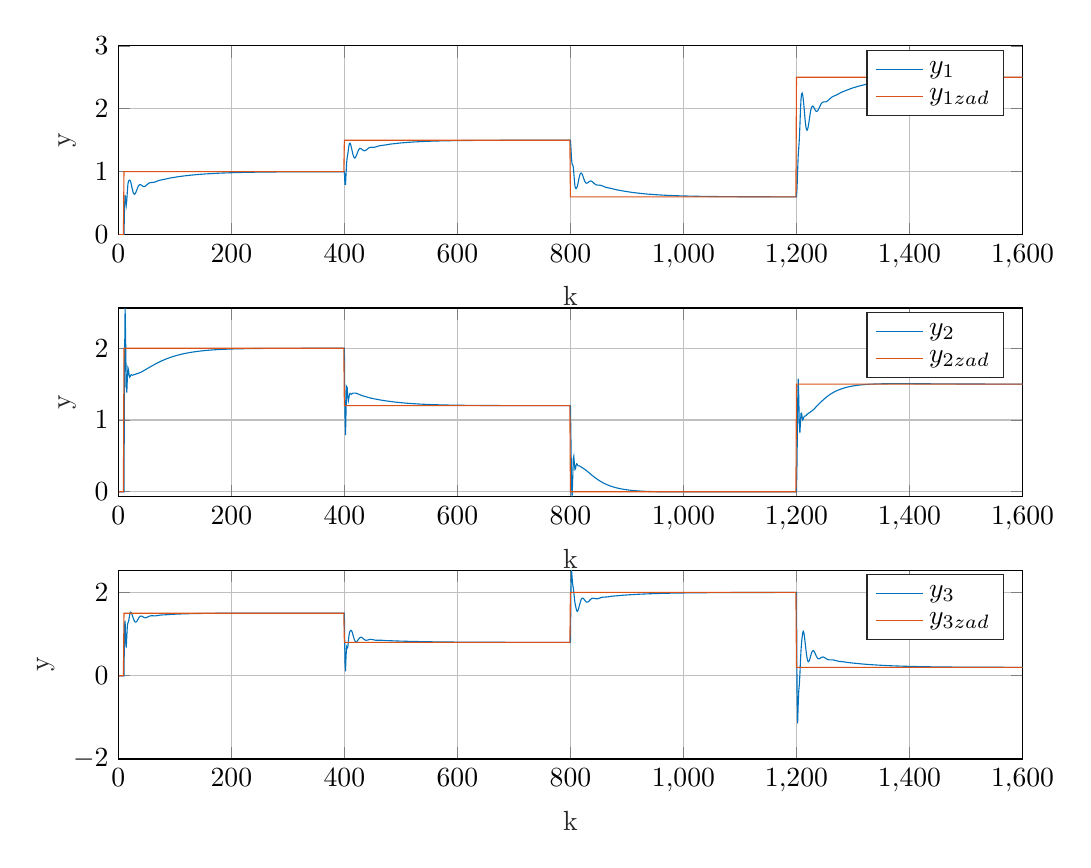
\begin{tikzpicture}

\begin{axis}[%
width=4.521in,
height=0.944in,
at={(0.758in,3.103in)},
scale only axis,
xmin=0,
xmax=1600,
xlabel style={font=\color{white!15!black}},
xlabel={k},
ymin=0,
ymax=3,
ylabel style={font=\color{white!15!black}},
ylabel={y},
axis background/.style={fill=white},
xmajorgrids,
ymajorgrids,
legend style={legend cell align=left, align=left, draw=white!15!black}
]
\addplot [color=mycolor1]
  table[row sep=crcr]{%
1	0\\
2	0\\
3	0\\
4	0\\
5	0\\
6	0\\
7	0\\
8	0\\
9	0\\
10	0\\
11	0.44309\\
12	0.63186\\
13	0.53891\\
14	0.46662\\
15	0.54728\\
16	0.69531\\
17	0.80365\\
18	0.84995\\
19	0.86325\\
20	0.86563\\
21	0.85778\\
22	0.83437\\
23	0.79682\\
24	0.75293\\
25	0.71124\\
26	0.67741\\
27	0.65418\\
28	0.64245\\
29	0.64204\\
30	0.65181\\
31	0.66959\\
32	0.69249\\
33	0.71737\\
34	0.74135\\
35	0.76212\\
36	0.77812\\
37	0.78862\\
38	0.7936\\
39	0.79373\\
40	0.79014\\
41	0.78422\\
42	0.77744\\
43	0.77116\\
44	0.76646\\
45	0.76405\\
46	0.76429\\
47	0.76716\\
48	0.7723\\
49	0.77918\\
50	0.7871\\
51	0.79535\\
52	0.80329\\
53	0.8104\\
54	0.81634\\
55	0.82095\\
56	0.82424\\
57	0.82638\\
58	0.82765\\
59	0.82837\\
60	0.82888\\
61	0.82949\\
62	0.83045\\
63	0.83192\\
64	0.83396\\
65	0.83658\\
66	0.83967\\
67	0.84312\\
68	0.84676\\
69	0.85043\\
70	0.85398\\
71	0.8573\\
72	0.86031\\
73	0.86299\\
74	0.86533\\
75	0.86738\\
76	0.8692\\
77	0.87088\\
78	0.87249\\
79	0.87411\\
80	0.87578\\
81	0.87755\\
82	0.87942\\
83	0.88141\\
84	0.88347\\
85	0.8856\\
86	0.88774\\
87	0.88986\\
88	0.89194\\
89	0.89393\\
90	0.89583\\
91	0.89763\\
92	0.89933\\
93	0.90095\\
94	0.9025\\
95	0.904\\
96	0.90546\\
97	0.90691\\
98	0.90835\\
99	0.9098\\
100	0.91126\\
101	0.91272\\
102	0.91419\\
103	0.91565\\
104	0.9171\\
105	0.91853\\
106	0.91993\\
107	0.9213\\
108	0.92263\\
109	0.92392\\
110	0.92518\\
111	0.9264\\
112	0.92759\\
113	0.92876\\
114	0.9299\\
115	0.93103\\
116	0.93215\\
117	0.93325\\
118	0.93435\\
119	0.93543\\
120	0.9365\\
121	0.93756\\
122	0.9386\\
123	0.93963\\
124	0.94064\\
125	0.94163\\
126	0.9426\\
127	0.94355\\
128	0.94448\\
129	0.94539\\
130	0.94629\\
131	0.94717\\
132	0.94803\\
133	0.94888\\
134	0.94972\\
135	0.95055\\
136	0.95137\\
137	0.95217\\
138	0.95296\\
139	0.95374\\
140	0.95451\\
141	0.95527\\
142	0.95601\\
143	0.95674\\
144	0.95746\\
145	0.95816\\
146	0.95886\\
147	0.95954\\
148	0.96021\\
149	0.96087\\
150	0.96151\\
151	0.96215\\
152	0.96278\\
153	0.96339\\
154	0.964\\
155	0.9646\\
156	0.96519\\
157	0.96577\\
158	0.96634\\
159	0.9669\\
160	0.96745\\
161	0.96799\\
162	0.96853\\
163	0.96905\\
164	0.96957\\
165	0.97007\\
166	0.97057\\
167	0.97106\\
168	0.97155\\
169	0.97202\\
170	0.97249\\
171	0.97295\\
172	0.9734\\
173	0.97384\\
174	0.97428\\
175	0.97471\\
176	0.97514\\
177	0.97555\\
178	0.97596\\
179	0.97636\\
180	0.97676\\
181	0.97715\\
182	0.97754\\
183	0.97791\\
184	0.97828\\
185	0.97865\\
186	0.97901\\
187	0.97936\\
188	0.97971\\
189	0.98005\\
190	0.98038\\
191	0.98071\\
192	0.98104\\
193	0.98136\\
194	0.98167\\
195	0.98198\\
196	0.98229\\
197	0.98259\\
198	0.98288\\
199	0.98317\\
200	0.98345\\
201	0.98373\\
202	0.98401\\
203	0.98428\\
204	0.98455\\
205	0.98481\\
206	0.98506\\
207	0.98532\\
208	0.98557\\
209	0.98581\\
210	0.98605\\
211	0.98629\\
212	0.98652\\
213	0.98675\\
214	0.98698\\
215	0.9872\\
216	0.98742\\
217	0.98763\\
218	0.98784\\
219	0.98805\\
220	0.98825\\
221	0.98845\\
222	0.98865\\
223	0.98884\\
224	0.98903\\
225	0.98922\\
226	0.9894\\
227	0.98958\\
228	0.98976\\
229	0.98994\\
230	0.99011\\
231	0.99028\\
232	0.99044\\
233	0.99061\\
234	0.99077\\
235	0.99093\\
236	0.99108\\
237	0.99123\\
238	0.99139\\
239	0.99153\\
240	0.99168\\
241	0.99182\\
242	0.99196\\
243	0.9921\\
244	0.99224\\
245	0.99237\\
246	0.9925\\
247	0.99263\\
248	0.99276\\
249	0.99288\\
250	0.993\\
251	0.99312\\
252	0.99324\\
253	0.99336\\
254	0.99347\\
255	0.99359\\
256	0.9937\\
257	0.99381\\
258	0.99391\\
259	0.99402\\
260	0.99412\\
261	0.99422\\
262	0.99432\\
263	0.99442\\
264	0.99452\\
265	0.99461\\
266	0.99471\\
267	0.9948\\
268	0.99489\\
269	0.99498\\
270	0.99506\\
271	0.99515\\
272	0.99523\\
273	0.99532\\
274	0.9954\\
275	0.99548\\
276	0.99556\\
277	0.99563\\
278	0.99571\\
279	0.99578\\
280	0.99586\\
281	0.99593\\
282	0.996\\
283	0.99607\\
284	0.99614\\
285	0.99621\\
286	0.99627\\
287	0.99634\\
288	0.9964\\
289	0.99647\\
290	0.99653\\
291	0.99659\\
292	0.99665\\
293	0.99671\\
294	0.99676\\
295	0.99682\\
296	0.99688\\
297	0.99693\\
298	0.99699\\
299	0.99704\\
300	0.99709\\
301	0.99714\\
302	0.99719\\
303	0.99724\\
304	0.99729\\
305	0.99734\\
306	0.99739\\
307	0.99743\\
308	0.99748\\
309	0.99752\\
310	0.99757\\
311	0.99761\\
312	0.99765\\
313	0.9977\\
314	0.99774\\
315	0.99778\\
316	0.99782\\
317	0.99786\\
318	0.9979\\
319	0.99793\\
320	0.99797\\
321	0.99801\\
322	0.99804\\
323	0.99808\\
324	0.99811\\
325	0.99815\\
326	0.99818\\
327	0.99821\\
328	0.99825\\
329	0.99828\\
330	0.99831\\
331	0.99834\\
332	0.99837\\
333	0.9984\\
334	0.99843\\
335	0.99846\\
336	0.99849\\
337	0.99851\\
338	0.99854\\
339	0.99857\\
340	0.99859\\
341	0.99862\\
342	0.99864\\
343	0.99867\\
344	0.99869\\
345	0.99872\\
346	0.99874\\
347	0.99876\\
348	0.99879\\
349	0.99881\\
350	0.99883\\
351	0.99885\\
352	0.99887\\
353	0.9989\\
354	0.99892\\
355	0.99894\\
356	0.99896\\
357	0.99898\\
358	0.999\\
359	0.99902\\
360	0.99904\\
361	0.99906\\
362	0.99907\\
363	0.99909\\
364	0.9991\\
365	0.99912\\
366	0.99913\\
367	0.99913\\
368	0.99914\\
369	0.99915\\
370	0.99916\\
371	0.99917\\
372	0.99918\\
373	0.99919\\
374	0.99921\\
375	0.99923\\
376	0.99925\\
377	0.99927\\
378	0.99929\\
379	0.99931\\
380	0.99933\\
381	0.99935\\
382	0.99936\\
383	0.99937\\
384	0.99938\\
385	0.99938\\
386	0.99939\\
387	0.9994\\
388	0.9994\\
389	0.99941\\
390	0.99942\\
391	0.99943\\
392	0.99944\\
393	0.99945\\
394	0.99946\\
395	0.99947\\
396	0.99949\\
397	0.9995\\
398	0.99951\\
399	0.99952\\
400	0.99953\\
401	0.79936\\
402	0.79742\\
403	0.9769\\
404	1.1442\\
405	1.2287\\
406	1.2809\\
407	1.3442\\
408	1.4089\\
409	1.4483\\
410	1.4538\\
411	1.4339\\
412	1.4004\\
413	1.3605\\
414	1.3189\\
415	1.2797\\
416	1.2477\\
417	1.2263\\
418	1.217\\
419	1.2196\\
420	1.232\\
421	1.2518\\
422	1.2757\\
423	1.3008\\
424	1.3243\\
425	1.3439\\
426	1.3583\\
427	1.3669\\
428	1.37\\
429	1.3682\\
430	1.363\\
431	1.3557\\
432	1.348\\
433	1.341\\
434	1.3359\\
435	1.3333\\
436	1.3334\\
437	1.3361\\
438	1.341\\
439	1.3475\\
440	1.355\\
441	1.3625\\
442	1.3696\\
443	1.3758\\
444	1.3807\\
445	1.3842\\
446	1.3864\\
447	1.3875\\
448	1.3877\\
449	1.3876\\
450	1.3873\\
451	1.3872\\
452	1.3875\\
453	1.3883\\
454	1.3898\\
455	1.3918\\
456	1.3944\\
457	1.3972\\
458	1.4002\\
459	1.4033\\
460	1.4061\\
461	1.4087\\
462	1.411\\
463	1.413\\
464	1.4146\\
465	1.416\\
466	1.4172\\
467	1.4182\\
468	1.4192\\
469	1.4202\\
470	1.4213\\
471	1.4226\\
472	1.4239\\
473	1.4254\\
474	1.4269\\
475	1.4285\\
476	1.4301\\
477	1.4317\\
478	1.4333\\
479	1.4347\\
480	1.4361\\
481	1.4374\\
482	1.4386\\
483	1.4397\\
484	1.4408\\
485	1.4418\\
486	1.4428\\
487	1.4437\\
488	1.4447\\
489	1.4457\\
490	1.4468\\
491	1.4478\\
492	1.4488\\
493	1.4498\\
494	1.4509\\
495	1.4519\\
496	1.4529\\
497	1.4538\\
498	1.4547\\
499	1.4556\\
500	1.4565\\
501	1.4573\\
502	1.4581\\
503	1.4589\\
504	1.4596\\
505	1.4604\\
506	1.4611\\
507	1.4619\\
508	1.4626\\
509	1.4633\\
510	1.4641\\
511	1.4648\\
512	1.4655\\
513	1.4661\\
514	1.4668\\
515	1.4675\\
516	1.4681\\
517	1.4687\\
518	1.4693\\
519	1.4699\\
520	1.4705\\
521	1.4711\\
522	1.4716\\
523	1.4722\\
524	1.4727\\
525	1.4732\\
526	1.4737\\
527	1.4742\\
528	1.4747\\
529	1.4752\\
530	1.4757\\
531	1.4762\\
532	1.4767\\
533	1.4771\\
534	1.4776\\
535	1.478\\
536	1.4784\\
537	1.4788\\
538	1.4792\\
539	1.4797\\
540	1.48\\
541	1.4804\\
542	1.4808\\
543	1.4812\\
544	1.4815\\
545	1.4819\\
546	1.4823\\
547	1.4826\\
548	1.4829\\
549	1.4833\\
550	1.4836\\
551	1.4839\\
552	1.4842\\
553	1.4845\\
554	1.4848\\
555	1.4851\\
556	1.4854\\
557	1.4857\\
558	1.486\\
559	1.4862\\
560	1.4865\\
561	1.4868\\
562	1.487\\
563	1.4873\\
564	1.4875\\
565	1.4878\\
566	1.488\\
567	1.4882\\
568	1.4885\\
569	1.4887\\
570	1.4889\\
571	1.4891\\
572	1.4893\\
573	1.4895\\
574	1.4897\\
575	1.4899\\
576	1.4901\\
577	1.4903\\
578	1.4905\\
579	1.4907\\
580	1.4909\\
581	1.4911\\
582	1.4912\\
583	1.4914\\
584	1.4916\\
585	1.4917\\
586	1.4919\\
587	1.492\\
588	1.4922\\
589	1.4924\\
590	1.4925\\
591	1.4926\\
592	1.4928\\
593	1.4929\\
594	1.4931\\
595	1.4932\\
596	1.4933\\
597	1.4935\\
598	1.4936\\
599	1.4937\\
600	1.4938\\
601	1.4939\\
602	1.4941\\
603	1.4942\\
604	1.4943\\
605	1.4944\\
606	1.4945\\
607	1.4946\\
608	1.4947\\
609	1.4948\\
610	1.4949\\
611	1.495\\
612	1.4951\\
613	1.4952\\
614	1.4953\\
615	1.4954\\
616	1.4955\\
617	1.4956\\
618	1.4957\\
619	1.4957\\
620	1.4958\\
621	1.4959\\
622	1.496\\
623	1.4961\\
624	1.4961\\
625	1.4962\\
626	1.4963\\
627	1.4963\\
628	1.4964\\
629	1.4965\\
630	1.4966\\
631	1.4966\\
632	1.4967\\
633	1.4967\\
634	1.4968\\
635	1.4969\\
636	1.4969\\
637	1.497\\
638	1.497\\
639	1.4971\\
640	1.4972\\
641	1.4972\\
642	1.4973\\
643	1.4973\\
644	1.4974\\
645	1.4974\\
646	1.4975\\
647	1.4975\\
648	1.4976\\
649	1.4976\\
650	1.4977\\
651	1.4977\\
652	1.4977\\
653	1.4978\\
654	1.4978\\
655	1.4979\\
656	1.4979\\
657	1.498\\
658	1.498\\
659	1.498\\
660	1.4981\\
661	1.4981\\
662	1.4981\\
663	1.4982\\
664	1.4982\\
665	1.4982\\
666	1.4983\\
667	1.4983\\
668	1.4983\\
669	1.4984\\
670	1.4984\\
671	1.4984\\
672	1.4985\\
673	1.4985\\
674	1.4985\\
675	1.4986\\
676	1.4986\\
677	1.4986\\
678	1.4986\\
679	1.4987\\
680	1.4987\\
681	1.4987\\
682	1.4987\\
683	1.4988\\
684	1.4988\\
685	1.4988\\
686	1.4988\\
687	1.4989\\
688	1.4989\\
689	1.4989\\
690	1.4989\\
691	1.4989\\
692	1.499\\
693	1.499\\
694	1.499\\
695	1.499\\
696	1.499\\
697	1.4991\\
698	1.4991\\
699	1.4991\\
700	1.4991\\
701	1.4991\\
702	1.4991\\
703	1.4992\\
704	1.4992\\
705	1.4992\\
706	1.4992\\
707	1.4992\\
708	1.4992\\
709	1.4993\\
710	1.4993\\
711	1.4993\\
712	1.4993\\
713	1.4993\\
714	1.4993\\
715	1.4993\\
716	1.4994\\
717	1.4994\\
718	1.4994\\
719	1.4994\\
720	1.4994\\
721	1.4994\\
722	1.4994\\
723	1.4994\\
724	1.4994\\
725	1.4995\\
726	1.4995\\
727	1.4995\\
728	1.4995\\
729	1.4995\\
730	1.4995\\
731	1.4995\\
732	1.4995\\
733	1.4995\\
734	1.4996\\
735	1.4996\\
736	1.4996\\
737	1.4996\\
738	1.4996\\
739	1.4996\\
740	1.4996\\
741	1.4996\\
742	1.4996\\
743	1.4996\\
744	1.4996\\
745	1.4996\\
746	1.4997\\
747	1.4997\\
748	1.4997\\
749	1.4997\\
750	1.4997\\
751	1.4997\\
752	1.4997\\
753	1.4997\\
754	1.4997\\
755	1.4997\\
756	1.4997\\
757	1.4997\\
758	1.4997\\
759	1.4997\\
760	1.4997\\
761	1.4997\\
762	1.4997\\
763	1.4997\\
764	1.4997\\
765	1.4997\\
766	1.4997\\
767	1.4998\\
768	1.4998\\
769	1.4998\\
770	1.4998\\
771	1.4998\\
772	1.4998\\
773	1.4998\\
774	1.4998\\
775	1.4998\\
776	1.4998\\
777	1.4998\\
778	1.4998\\
779	1.4998\\
780	1.4998\\
781	1.4998\\
782	1.4998\\
783	1.4998\\
784	1.4998\\
785	1.4998\\
786	1.4998\\
787	1.4998\\
788	1.4998\\
789	1.4999\\
790	1.4999\\
791	1.4999\\
792	1.4999\\
793	1.4999\\
794	1.4999\\
795	1.4999\\
796	1.4999\\
797	1.4999\\
798	1.4999\\
799	1.4999\\
800	1.4999\\
801	1.3599\\
802	1.1975\\
803	1.1177\\
804	1.1076\\
805	1.0752\\
806	0.97942\\
807	0.86097\\
808	0.77477\\
809	0.73657\\
810	0.73087\\
811	0.74161\\
812	0.76442\\
813	0.7996\\
814	0.84378\\
815	0.88946\\
816	0.9291\\
817	0.95801\\
818	0.97437\\
819	0.97823\\
820	0.97076\\
821	0.95405\\
822	0.93096\\
823	0.90479\\
824	0.87875\\
825	0.85554\\
826	0.83708\\
827	0.82442\\
828	0.81778\\
829	0.81663\\
830	0.81988\\
831	0.82608\\
832	0.83365\\
833	0.84107\\
834	0.84709\\
835	0.85081\\
836	0.85174\\
837	0.84979\\
838	0.84524\\
839	0.83863\\
840	0.83067\\
841	0.82213\\
842	0.81371\\
843	0.80604\\
844	0.79953\\
845	0.79441\\
846	0.79072\\
847	0.78832\\
848	0.78694\\
849	0.78624\\
850	0.78586\\
851	0.78544\\
852	0.78471\\
853	0.78346\\
854	0.78159\\
855	0.77909\\
856	0.77602\\
857	0.77252\\
858	0.76875\\
859	0.76489\\
860	0.76111\\
861	0.75753\\
862	0.75426\\
863	0.75134\\
864	0.74878\\
865	0.74654\\
866	0.74455\\
867	0.74274\\
868	0.74102\\
869	0.73931\\
870	0.73755\\
871	0.73569\\
872	0.7337\\
873	0.7316\\
874	0.72939\\
875	0.7271\\
876	0.72478\\
877	0.72246\\
878	0.72019\\
879	0.71799\\
880	0.71588\\
881	0.71388\\
882	0.71198\\
883	0.71017\\
884	0.70844\\
885	0.70677\\
886	0.70514\\
887	0.70353\\
888	0.70192\\
889	0.70031\\
890	0.69869\\
891	0.69706\\
892	0.69543\\
893	0.69379\\
894	0.69217\\
895	0.69057\\
896	0.68899\\
897	0.68745\\
898	0.68594\\
899	0.68448\\
900	0.68306\\
901	0.68167\\
902	0.68032\\
903	0.67899\\
904	0.67769\\
905	0.67641\\
906	0.67514\\
907	0.67389\\
908	0.67265\\
909	0.67142\\
910	0.67021\\
911	0.66901\\
912	0.66782\\
913	0.66665\\
914	0.66551\\
915	0.66438\\
916	0.66328\\
917	0.66219\\
918	0.66113\\
919	0.66009\\
920	0.65907\\
921	0.65806\\
922	0.65708\\
923	0.65611\\
924	0.65515\\
925	0.65421\\
926	0.65328\\
927	0.65237\\
928	0.65147\\
929	0.65058\\
930	0.64971\\
931	0.64885\\
932	0.648\\
933	0.64717\\
934	0.64636\\
935	0.64556\\
936	0.64477\\
937	0.644\\
938	0.64324\\
939	0.64249\\
940	0.64176\\
941	0.64104\\
942	0.64033\\
943	0.63963\\
944	0.63894\\
945	0.63827\\
946	0.6376\\
947	0.63695\\
948	0.63631\\
949	0.63567\\
950	0.63505\\
951	0.63444\\
952	0.63384\\
953	0.63325\\
954	0.63267\\
955	0.6321\\
956	0.63154\\
957	0.63099\\
958	0.63045\\
959	0.62992\\
960	0.6294\\
961	0.62889\\
962	0.62838\\
963	0.62788\\
964	0.6274\\
965	0.62692\\
966	0.62645\\
967	0.62598\\
968	0.62553\\
969	0.62508\\
970	0.62464\\
971	0.62421\\
972	0.62378\\
973	0.62336\\
974	0.62295\\
975	0.62255\\
976	0.62215\\
977	0.62176\\
978	0.62138\\
979	0.62101\\
980	0.62064\\
981	0.62027\\
982	0.61992\\
983	0.61956\\
984	0.61922\\
985	0.61888\\
986	0.61855\\
987	0.61822\\
988	0.6179\\
989	0.61758\\
990	0.61727\\
991	0.61697\\
992	0.61667\\
993	0.61637\\
994	0.61608\\
995	0.6158\\
996	0.61552\\
997	0.61525\\
998	0.61498\\
999	0.61471\\
1000	0.61445\\
1001	0.6142\\
1002	0.61394\\
1003	0.6137\\
1004	0.61346\\
1005	0.61322\\
1006	0.61298\\
1007	0.61275\\
1008	0.61253\\
1009	0.6123\\
1010	0.61209\\
1011	0.61187\\
1012	0.61166\\
1013	0.61145\\
1014	0.61125\\
1015	0.61105\\
1016	0.61085\\
1017	0.61066\\
1018	0.61047\\
1019	0.61029\\
1020	0.6101\\
1021	0.60992\\
1022	0.60975\\
1023	0.60957\\
1024	0.6094\\
1025	0.60924\\
1026	0.60907\\
1027	0.60891\\
1028	0.60875\\
1029	0.6086\\
1030	0.60844\\
1031	0.60829\\
1032	0.60815\\
1033	0.608\\
1034	0.60786\\
1035	0.60772\\
1036	0.60758\\
1037	0.60745\\
1038	0.60731\\
1039	0.60718\\
1040	0.60705\\
1041	0.60693\\
1042	0.60681\\
1043	0.60668\\
1044	0.60656\\
1045	0.60645\\
1046	0.60633\\
1047	0.60622\\
1048	0.60611\\
1049	0.606\\
1050	0.60589\\
1051	0.60579\\
1052	0.60568\\
1053	0.60558\\
1054	0.60548\\
1055	0.60538\\
1056	0.60529\\
1057	0.60519\\
1058	0.6051\\
1059	0.60501\\
1060	0.60492\\
1061	0.60483\\
1062	0.60475\\
1063	0.60466\\
1064	0.60458\\
1065	0.6045\\
1066	0.60442\\
1067	0.60434\\
1068	0.60426\\
1069	0.60418\\
1070	0.60411\\
1071	0.60403\\
1072	0.60396\\
1073	0.60389\\
1074	0.60382\\
1075	0.60375\\
1076	0.60368\\
1077	0.60362\\
1078	0.60355\\
1079	0.60349\\
1080	0.60343\\
1081	0.60336\\
1082	0.6033\\
1083	0.60324\\
1084	0.60319\\
1085	0.60313\\
1086	0.60307\\
1087	0.60302\\
1088	0.60296\\
1089	0.60291\\
1090	0.60286\\
1091	0.6028\\
1092	0.60275\\
1093	0.6027\\
1094	0.60265\\
1095	0.60261\\
1096	0.60256\\
1097	0.60251\\
1098	0.60247\\
1099	0.60242\\
1100	0.60238\\
1101	0.60233\\
1102	0.60229\\
1103	0.60225\\
1104	0.60221\\
1105	0.60217\\
1106	0.60213\\
1107	0.60209\\
1108	0.60205\\
1109	0.60201\\
1110	0.60198\\
1111	0.60194\\
1112	0.6019\\
1113	0.60187\\
1114	0.60183\\
1115	0.6018\\
1116	0.60177\\
1117	0.60173\\
1118	0.6017\\
1119	0.60167\\
1120	0.60164\\
1121	0.60161\\
1122	0.60158\\
1123	0.60155\\
1124	0.60152\\
1125	0.60149\\
1126	0.60146\\
1127	0.60143\\
1128	0.60141\\
1129	0.60138\\
1130	0.60135\\
1131	0.60133\\
1132	0.6013\\
1133	0.60128\\
1134	0.60125\\
1135	0.60123\\
1136	0.60121\\
1137	0.60118\\
1138	0.60116\\
1139	0.60114\\
1140	0.60111\\
1141	0.60109\\
1142	0.60107\\
1143	0.60105\\
1144	0.60103\\
1145	0.60101\\
1146	0.60099\\
1147	0.60097\\
1148	0.60095\\
1149	0.60093\\
1150	0.60091\\
1151	0.6009\\
1152	0.60088\\
1153	0.60086\\
1154	0.60085\\
1155	0.60083\\
1156	0.60082\\
1157	0.60081\\
1158	0.60081\\
1159	0.6008\\
1160	0.60079\\
1161	0.60078\\
1162	0.60077\\
1163	0.60076\\
1164	0.60075\\
1165	0.60073\\
1166	0.60071\\
1167	0.60069\\
1168	0.60067\\
1169	0.60065\\
1170	0.60063\\
1171	0.60061\\
1172	0.6006\\
1173	0.60059\\
1174	0.60058\\
1175	0.60057\\
1176	0.60057\\
1177	0.60056\\
1178	0.60056\\
1179	0.60055\\
1180	0.60055\\
1181	0.60054\\
1182	0.60053\\
1183	0.60052\\
1184	0.6005\\
1185	0.60049\\
1186	0.60048\\
1187	0.60047\\
1188	0.60045\\
1189	0.60044\\
1190	0.60043\\
1191	0.60043\\
1192	0.60042\\
1193	0.60041\\
1194	0.60041\\
1195	0.6004\\
1196	0.6004\\
1197	0.60039\\
1198	0.60039\\
1199	0.60038\\
1200	0.60037\\
1201	0.74337\\
1202	1.0123\\
1203	1.2436\\
1204	1.3761\\
1205	1.5115\\
1206	1.7241\\
1207	1.9658\\
1208	2.1483\\
1209	2.2362\\
1210	2.2491\\
1211	2.216\\
1212	2.1511\\
1213	2.0605\\
1214	1.9544\\
1215	1.8491\\
1216	1.7598\\
1217	1.6967\\
1218	1.6638\\
1219	1.6605\\
1220	1.6836\\
1221	1.7273\\
1222	1.7845\\
1223	1.8473\\
1224	1.9084\\
1225	1.9616\\
1226	2.0028\\
1227	2.0298\\
1228	2.0427\\
1229	2.0428\\
1230	2.0331\\
1231	2.0171\\
1232	1.9987\\
1233	1.9812\\
1234	1.9675\\
1235	1.9597\\
1236	1.9585\\
1237	1.9642\\
1238	1.9758\\
1239	1.992\\
1240	2.011\\
1241	2.031\\
1242	2.0504\\
1243	2.0678\\
1244	2.0822\\
1245	2.0933\\
1246	2.101\\
1247	2.1057\\
1248	2.1081\\
1249	2.1091\\
1250	2.1095\\
1251	2.1102\\
1252	2.1117\\
1253	2.1145\\
1254	2.1187\\
1255	2.1245\\
1256	2.1316\\
1257	2.1396\\
1258	2.1482\\
1259	2.1569\\
1260	2.1653\\
1261	2.1732\\
1262	2.1804\\
1263	2.1866\\
1264	2.1921\\
1265	2.1968\\
1266	2.2009\\
1267	2.2047\\
1268	2.2083\\
1269	2.2119\\
1270	2.2156\\
1271	2.2196\\
1272	2.2239\\
1273	2.2285\\
1274	2.2333\\
1275	2.2383\\
1276	2.2434\\
1277	2.2484\\
1278	2.2533\\
1279	2.258\\
1280	2.2625\\
1281	2.2668\\
1282	2.2708\\
1283	2.2746\\
1284	2.2782\\
1285	2.2817\\
1286	2.2851\\
1287	2.2885\\
1288	2.2919\\
1289	2.2953\\
1290	2.2987\\
1291	2.3021\\
1292	2.3056\\
1293	2.3091\\
1294	2.3125\\
1295	2.3159\\
1296	2.3192\\
1297	2.3224\\
1298	2.3256\\
1299	2.3286\\
1300	2.3316\\
1301	2.3345\\
1302	2.3373\\
1303	2.34\\
1304	2.3427\\
1305	2.3454\\
1306	2.348\\
1307	2.3506\\
1308	2.3532\\
1309	2.3558\\
1310	2.3583\\
1311	2.3608\\
1312	2.3632\\
1313	2.3657\\
1314	2.368\\
1315	2.3704\\
1316	2.3726\\
1317	2.3749\\
1318	2.3771\\
1319	2.3792\\
1320	2.3813\\
1321	2.3834\\
1322	2.3854\\
1323	2.3874\\
1324	2.3893\\
1325	2.3913\\
1326	2.3932\\
1327	2.395\\
1328	2.3969\\
1329	2.3987\\
1330	2.4005\\
1331	2.4022\\
1332	2.404\\
1333	2.4057\\
1334	2.4073\\
1335	2.409\\
1336	2.4106\\
1337	2.4121\\
1338	2.4137\\
1339	2.4152\\
1340	2.4167\\
1341	2.4182\\
1342	2.4196\\
1343	2.421\\
1344	2.4224\\
1345	2.4238\\
1346	2.4251\\
1347	2.4265\\
1348	2.4278\\
1349	2.429\\
1350	2.4303\\
1351	2.4315\\
1352	2.4327\\
1353	2.4339\\
1354	2.4351\\
1355	2.4363\\
1356	2.4374\\
1357	2.4385\\
1358	2.4396\\
1359	2.4407\\
1360	2.4417\\
1361	2.4427\\
1362	2.4438\\
1363	2.4448\\
1364	2.4457\\
1365	2.4467\\
1366	2.4476\\
1367	2.4486\\
1368	2.4495\\
1369	2.4504\\
1370	2.4513\\
1371	2.4521\\
1372	2.453\\
1373	2.4538\\
1374	2.4547\\
1375	2.4555\\
1376	2.4563\\
1377	2.457\\
1378	2.4578\\
1379	2.4585\\
1380	2.4593\\
1381	2.46\\
1382	2.4607\\
1383	2.4614\\
1384	2.4621\\
1385	2.4628\\
1386	2.4635\\
1387	2.4641\\
1388	2.4647\\
1389	2.4654\\
1390	2.466\\
1391	2.4666\\
1392	2.4672\\
1393	2.4678\\
1394	2.4684\\
1395	2.4689\\
1396	2.4695\\
1397	2.47\\
1398	2.4706\\
1399	2.4711\\
1400	2.4716\\
1401	2.4721\\
1402	2.4726\\
1403	2.4731\\
1404	2.4736\\
1405	2.4741\\
1406	2.4745\\
1407	2.475\\
1408	2.4754\\
1409	2.4759\\
1410	2.4763\\
1411	2.4767\\
1412	2.4771\\
1413	2.4776\\
1414	2.478\\
1415	2.4783\\
1416	2.4787\\
1417	2.4791\\
1418	2.4795\\
1419	2.4799\\
1420	2.4802\\
1421	2.4806\\
1422	2.4809\\
1423	2.4813\\
1424	2.4816\\
1425	2.4819\\
1426	2.4823\\
1427	2.4826\\
1428	2.4829\\
1429	2.4832\\
1430	2.4835\\
1431	2.4838\\
1432	2.4841\\
1433	2.4844\\
1434	2.4847\\
1435	2.4849\\
1436	2.4852\\
1437	2.4855\\
1438	2.4857\\
1439	2.486\\
1440	2.4862\\
1441	2.4865\\
1442	2.4867\\
1443	2.487\\
1444	2.4872\\
1445	2.4874\\
1446	2.4877\\
1447	2.4879\\
1448	2.4881\\
1449	2.4883\\
1450	2.4885\\
1451	2.4887\\
1452	2.4889\\
1453	2.4891\\
1454	2.4893\\
1455	2.4895\\
1456	2.4897\\
1457	2.4899\\
1458	2.4901\\
1459	2.4902\\
1460	2.4904\\
1461	2.4906\\
1462	2.4908\\
1463	2.4909\\
1464	2.4911\\
1465	2.4913\\
1466	2.4914\\
1467	2.4916\\
1468	2.4917\\
1469	2.4919\\
1470	2.492\\
1471	2.4922\\
1472	2.4923\\
1473	2.4924\\
1474	2.4926\\
1475	2.4927\\
1476	2.4928\\
1477	2.493\\
1478	2.4931\\
1479	2.4932\\
1480	2.4933\\
1481	2.4935\\
1482	2.4936\\
1483	2.4937\\
1484	2.4938\\
1485	2.4939\\
1486	2.494\\
1487	2.4941\\
1488	2.4943\\
1489	2.4944\\
1490	2.4945\\
1491	2.4946\\
1492	2.4947\\
1493	2.4948\\
1494	2.4949\\
1495	2.4949\\
1496	2.495\\
1497	2.4951\\
1498	2.4952\\
1499	2.4953\\
1500	2.4954\\
1501	2.4955\\
1502	2.4956\\
1503	2.4956\\
1504	2.4957\\
1505	2.4958\\
1506	2.4959\\
1507	2.496\\
1508	2.496\\
1509	2.4961\\
1510	2.4962\\
1511	2.4963\\
1512	2.4963\\
1513	2.4964\\
1514	2.4965\\
1515	2.4965\\
1516	2.4966\\
1517	2.4967\\
1518	2.4967\\
1519	2.4968\\
1520	2.4968\\
1521	2.4969\\
1522	2.497\\
1523	2.497\\
1524	2.4971\\
1525	2.4971\\
1526	2.4972\\
1527	2.4972\\
1528	2.4973\\
1529	2.4973\\
1530	2.4974\\
1531	2.4974\\
1532	2.4975\\
1533	2.4975\\
1534	2.4976\\
1535	2.4976\\
1536	2.4977\\
1537	2.4977\\
1538	2.4978\\
1539	2.4978\\
1540	2.4979\\
1541	2.4979\\
1542	2.4979\\
1543	2.498\\
1544	2.498\\
1545	2.4981\\
1546	2.4981\\
1547	2.4981\\
1548	2.4982\\
1549	2.4982\\
1550	2.4982\\
1551	2.4983\\
1552	2.4983\\
1553	2.4983\\
1554	2.4984\\
1555	2.4984\\
1556	2.4984\\
1557	2.4984\\
1558	2.4984\\
1559	2.4985\\
1560	2.4985\\
1561	2.4985\\
1562	2.4985\\
1563	2.4985\\
1564	2.4986\\
1565	2.4986\\
1566	2.4986\\
1567	2.4987\\
1568	2.4987\\
1569	2.4988\\
1570	2.4988\\
1571	2.4988\\
1572	2.4989\\
1573	2.4989\\
1574	2.4989\\
1575	2.4989\\
1576	2.4989\\
1577	2.4989\\
1578	2.4989\\
1579	2.4989\\
1580	2.4989\\
1581	2.499\\
1582	2.499\\
1583	2.499\\
1584	2.499\\
1585	2.4991\\
1586	2.4991\\
1587	2.4991\\
1588	2.4991\\
1589	2.4992\\
1590	2.4992\\
1591	2.4992\\
1592	2.4992\\
1593	2.4992\\
1594	2.4992\\
1595	2.4992\\
1596	2.4992\\
1597	2.4992\\
1598	2.4993\\
1599	2.4993\\
1600	2.4993\\
};
\addlegendentry{$\text{y}_\text{1}$}

\addplot [color=mycolor2]
  table[row sep=crcr]{%
1	0\\
2	0\\
3	0\\
4	0\\
5	0\\
6	0\\
7	0\\
8	0\\
9	0\\
10	1\\
11	1\\
12	1\\
13	1\\
14	1\\
15	1\\
16	1\\
17	1\\
18	1\\
19	1\\
20	1\\
21	1\\
22	1\\
23	1\\
24	1\\
25	1\\
26	1\\
27	1\\
28	1\\
29	1\\
30	1\\
31	1\\
32	1\\
33	1\\
34	1\\
35	1\\
36	1\\
37	1\\
38	1\\
39	1\\
40	1\\
41	1\\
42	1\\
43	1\\
44	1\\
45	1\\
46	1\\
47	1\\
48	1\\
49	1\\
50	1\\
51	1\\
52	1\\
53	1\\
54	1\\
55	1\\
56	1\\
57	1\\
58	1\\
59	1\\
60	1\\
61	1\\
62	1\\
63	1\\
64	1\\
65	1\\
66	1\\
67	1\\
68	1\\
69	1\\
70	1\\
71	1\\
72	1\\
73	1\\
74	1\\
75	1\\
76	1\\
77	1\\
78	1\\
79	1\\
80	1\\
81	1\\
82	1\\
83	1\\
84	1\\
85	1\\
86	1\\
87	1\\
88	1\\
89	1\\
90	1\\
91	1\\
92	1\\
93	1\\
94	1\\
95	1\\
96	1\\
97	1\\
98	1\\
99	1\\
100	1\\
101	1\\
102	1\\
103	1\\
104	1\\
105	1\\
106	1\\
107	1\\
108	1\\
109	1\\
110	1\\
111	1\\
112	1\\
113	1\\
114	1\\
115	1\\
116	1\\
117	1\\
118	1\\
119	1\\
120	1\\
121	1\\
122	1\\
123	1\\
124	1\\
125	1\\
126	1\\
127	1\\
128	1\\
129	1\\
130	1\\
131	1\\
132	1\\
133	1\\
134	1\\
135	1\\
136	1\\
137	1\\
138	1\\
139	1\\
140	1\\
141	1\\
142	1\\
143	1\\
144	1\\
145	1\\
146	1\\
147	1\\
148	1\\
149	1\\
150	1\\
151	1\\
152	1\\
153	1\\
154	1\\
155	1\\
156	1\\
157	1\\
158	1\\
159	1\\
160	1\\
161	1\\
162	1\\
163	1\\
164	1\\
165	1\\
166	1\\
167	1\\
168	1\\
169	1\\
170	1\\
171	1\\
172	1\\
173	1\\
174	1\\
175	1\\
176	1\\
177	1\\
178	1\\
179	1\\
180	1\\
181	1\\
182	1\\
183	1\\
184	1\\
185	1\\
186	1\\
187	1\\
188	1\\
189	1\\
190	1\\
191	1\\
192	1\\
193	1\\
194	1\\
195	1\\
196	1\\
197	1\\
198	1\\
199	1\\
200	1\\
201	1\\
202	1\\
203	1\\
204	1\\
205	1\\
206	1\\
207	1\\
208	1\\
209	1\\
210	1\\
211	1\\
212	1\\
213	1\\
214	1\\
215	1\\
216	1\\
217	1\\
218	1\\
219	1\\
220	1\\
221	1\\
222	1\\
223	1\\
224	1\\
225	1\\
226	1\\
227	1\\
228	1\\
229	1\\
230	1\\
231	1\\
232	1\\
233	1\\
234	1\\
235	1\\
236	1\\
237	1\\
238	1\\
239	1\\
240	1\\
241	1\\
242	1\\
243	1\\
244	1\\
245	1\\
246	1\\
247	1\\
248	1\\
249	1\\
250	1\\
251	1\\
252	1\\
253	1\\
254	1\\
255	1\\
256	1\\
257	1\\
258	1\\
259	1\\
260	1\\
261	1\\
262	1\\
263	1\\
264	1\\
265	1\\
266	1\\
267	1\\
268	1\\
269	1\\
270	1\\
271	1\\
272	1\\
273	1\\
274	1\\
275	1\\
276	1\\
277	1\\
278	1\\
279	1\\
280	1\\
281	1\\
282	1\\
283	1\\
284	1\\
285	1\\
286	1\\
287	1\\
288	1\\
289	1\\
290	1\\
291	1\\
292	1\\
293	1\\
294	1\\
295	1\\
296	1\\
297	1\\
298	1\\
299	1\\
300	1\\
301	1\\
302	1\\
303	1\\
304	1\\
305	1\\
306	1\\
307	1\\
308	1\\
309	1\\
310	1\\
311	1\\
312	1\\
313	1\\
314	1\\
315	1\\
316	1\\
317	1\\
318	1\\
319	1\\
320	1\\
321	1\\
322	1\\
323	1\\
324	1\\
325	1\\
326	1\\
327	1\\
328	1\\
329	1\\
330	1\\
331	1\\
332	1\\
333	1\\
334	1\\
335	1\\
336	1\\
337	1\\
338	1\\
339	1\\
340	1\\
341	1\\
342	1\\
343	1\\
344	1\\
345	1\\
346	1\\
347	1\\
348	1\\
349	1\\
350	1\\
351	1\\
352	1\\
353	1\\
354	1\\
355	1\\
356	1\\
357	1\\
358	1\\
359	1\\
360	1\\
361	1\\
362	1\\
363	1\\
364	1\\
365	1\\
366	1\\
367	1\\
368	1\\
369	1\\
370	1\\
371	1\\
372	1\\
373	1\\
374	1\\
375	1\\
376	1\\
377	1\\
378	1\\
379	1\\
380	1\\
381	1\\
382	1\\
383	1\\
384	1\\
385	1\\
386	1\\
387	1\\
388	1\\
389	1\\
390	1\\
391	1\\
392	1\\
393	1\\
394	1\\
395	1\\
396	1\\
397	1\\
398	1\\
399	1\\
400	1.5\\
401	1.5\\
402	1.5\\
403	1.5\\
404	1.5\\
405	1.5\\
406	1.5\\
407	1.5\\
408	1.5\\
409	1.5\\
410	1.5\\
411	1.5\\
412	1.5\\
413	1.5\\
414	1.5\\
415	1.5\\
416	1.5\\
417	1.5\\
418	1.5\\
419	1.5\\
420	1.5\\
421	1.5\\
422	1.5\\
423	1.5\\
424	1.5\\
425	1.5\\
426	1.5\\
427	1.5\\
428	1.5\\
429	1.5\\
430	1.5\\
431	1.5\\
432	1.5\\
433	1.5\\
434	1.5\\
435	1.5\\
436	1.5\\
437	1.5\\
438	1.5\\
439	1.5\\
440	1.5\\
441	1.5\\
442	1.5\\
443	1.5\\
444	1.5\\
445	1.5\\
446	1.5\\
447	1.5\\
448	1.5\\
449	1.5\\
450	1.5\\
451	1.5\\
452	1.5\\
453	1.5\\
454	1.5\\
455	1.5\\
456	1.5\\
457	1.5\\
458	1.5\\
459	1.5\\
460	1.5\\
461	1.5\\
462	1.5\\
463	1.5\\
464	1.5\\
465	1.5\\
466	1.5\\
467	1.5\\
468	1.5\\
469	1.5\\
470	1.5\\
471	1.5\\
472	1.5\\
473	1.5\\
474	1.5\\
475	1.5\\
476	1.5\\
477	1.5\\
478	1.5\\
479	1.5\\
480	1.5\\
481	1.5\\
482	1.5\\
483	1.5\\
484	1.5\\
485	1.5\\
486	1.5\\
487	1.5\\
488	1.5\\
489	1.5\\
490	1.5\\
491	1.5\\
492	1.5\\
493	1.5\\
494	1.5\\
495	1.5\\
496	1.5\\
497	1.5\\
498	1.5\\
499	1.5\\
500	1.5\\
501	1.5\\
502	1.5\\
503	1.5\\
504	1.5\\
505	1.5\\
506	1.5\\
507	1.5\\
508	1.5\\
509	1.5\\
510	1.5\\
511	1.5\\
512	1.5\\
513	1.5\\
514	1.5\\
515	1.5\\
516	1.5\\
517	1.5\\
518	1.5\\
519	1.5\\
520	1.5\\
521	1.5\\
522	1.5\\
523	1.5\\
524	1.5\\
525	1.5\\
526	1.5\\
527	1.5\\
528	1.5\\
529	1.5\\
530	1.5\\
531	1.5\\
532	1.5\\
533	1.5\\
534	1.5\\
535	1.5\\
536	1.5\\
537	1.5\\
538	1.5\\
539	1.5\\
540	1.5\\
541	1.5\\
542	1.5\\
543	1.5\\
544	1.5\\
545	1.5\\
546	1.5\\
547	1.5\\
548	1.5\\
549	1.5\\
550	1.5\\
551	1.5\\
552	1.5\\
553	1.5\\
554	1.5\\
555	1.5\\
556	1.5\\
557	1.5\\
558	1.5\\
559	1.5\\
560	1.5\\
561	1.5\\
562	1.5\\
563	1.5\\
564	1.5\\
565	1.5\\
566	1.5\\
567	1.5\\
568	1.5\\
569	1.5\\
570	1.5\\
571	1.5\\
572	1.5\\
573	1.5\\
574	1.5\\
575	1.5\\
576	1.5\\
577	1.5\\
578	1.5\\
579	1.5\\
580	1.5\\
581	1.5\\
582	1.5\\
583	1.5\\
584	1.5\\
585	1.5\\
586	1.5\\
587	1.5\\
588	1.5\\
589	1.5\\
590	1.5\\
591	1.5\\
592	1.5\\
593	1.5\\
594	1.5\\
595	1.5\\
596	1.5\\
597	1.5\\
598	1.5\\
599	1.5\\
600	1.5\\
601	1.5\\
602	1.5\\
603	1.5\\
604	1.5\\
605	1.5\\
606	1.5\\
607	1.5\\
608	1.5\\
609	1.5\\
610	1.5\\
611	1.5\\
612	1.5\\
613	1.5\\
614	1.5\\
615	1.5\\
616	1.5\\
617	1.5\\
618	1.5\\
619	1.5\\
620	1.5\\
621	1.5\\
622	1.5\\
623	1.5\\
624	1.5\\
625	1.5\\
626	1.5\\
627	1.5\\
628	1.5\\
629	1.5\\
630	1.5\\
631	1.5\\
632	1.5\\
633	1.5\\
634	1.5\\
635	1.5\\
636	1.5\\
637	1.5\\
638	1.5\\
639	1.5\\
640	1.5\\
641	1.5\\
642	1.5\\
643	1.5\\
644	1.5\\
645	1.5\\
646	1.5\\
647	1.5\\
648	1.5\\
649	1.5\\
650	1.5\\
651	1.5\\
652	1.5\\
653	1.5\\
654	1.5\\
655	1.5\\
656	1.5\\
657	1.5\\
658	1.5\\
659	1.5\\
660	1.5\\
661	1.5\\
662	1.5\\
663	1.5\\
664	1.5\\
665	1.5\\
666	1.5\\
667	1.5\\
668	1.5\\
669	1.5\\
670	1.5\\
671	1.5\\
672	1.5\\
673	1.5\\
674	1.5\\
675	1.5\\
676	1.5\\
677	1.5\\
678	1.5\\
679	1.5\\
680	1.5\\
681	1.5\\
682	1.5\\
683	1.5\\
684	1.5\\
685	1.5\\
686	1.5\\
687	1.5\\
688	1.5\\
689	1.5\\
690	1.5\\
691	1.5\\
692	1.5\\
693	1.5\\
694	1.5\\
695	1.5\\
696	1.5\\
697	1.5\\
698	1.5\\
699	1.5\\
700	1.5\\
701	1.5\\
702	1.5\\
703	1.5\\
704	1.5\\
705	1.5\\
706	1.5\\
707	1.5\\
708	1.5\\
709	1.5\\
710	1.5\\
711	1.5\\
712	1.5\\
713	1.5\\
714	1.5\\
715	1.5\\
716	1.5\\
717	1.5\\
718	1.5\\
719	1.5\\
720	1.5\\
721	1.5\\
722	1.5\\
723	1.5\\
724	1.5\\
725	1.5\\
726	1.5\\
727	1.5\\
728	1.5\\
729	1.5\\
730	1.5\\
731	1.5\\
732	1.5\\
733	1.5\\
734	1.5\\
735	1.5\\
736	1.5\\
737	1.5\\
738	1.5\\
739	1.5\\
740	1.5\\
741	1.5\\
742	1.5\\
743	1.5\\
744	1.5\\
745	1.5\\
746	1.5\\
747	1.5\\
748	1.5\\
749	1.5\\
750	1.5\\
751	1.5\\
752	1.5\\
753	1.5\\
754	1.5\\
755	1.5\\
756	1.5\\
757	1.5\\
758	1.5\\
759	1.5\\
760	1.5\\
761	1.5\\
762	1.5\\
763	1.5\\
764	1.5\\
765	1.5\\
766	1.5\\
767	1.5\\
768	1.5\\
769	1.5\\
770	1.5\\
771	1.5\\
772	1.5\\
773	1.5\\
774	1.5\\
775	1.5\\
776	1.5\\
777	1.5\\
778	1.5\\
779	1.5\\
780	1.5\\
781	1.5\\
782	1.5\\
783	1.5\\
784	1.5\\
785	1.5\\
786	1.5\\
787	1.5\\
788	1.5\\
789	1.5\\
790	1.5\\
791	1.5\\
792	1.5\\
793	1.5\\
794	1.5\\
795	1.5\\
796	1.5\\
797	1.5\\
798	1.5\\
799	1.5\\
800	0.6\\
801	0.6\\
802	0.6\\
803	0.6\\
804	0.6\\
805	0.6\\
806	0.6\\
807	0.6\\
808	0.6\\
809	0.6\\
810	0.6\\
811	0.6\\
812	0.6\\
813	0.6\\
814	0.6\\
815	0.6\\
816	0.6\\
817	0.6\\
818	0.6\\
819	0.6\\
820	0.6\\
821	0.6\\
822	0.6\\
823	0.6\\
824	0.6\\
825	0.6\\
826	0.6\\
827	0.6\\
828	0.6\\
829	0.6\\
830	0.6\\
831	0.6\\
832	0.6\\
833	0.6\\
834	0.6\\
835	0.6\\
836	0.6\\
837	0.6\\
838	0.6\\
839	0.6\\
840	0.6\\
841	0.6\\
842	0.6\\
843	0.6\\
844	0.6\\
845	0.6\\
846	0.6\\
847	0.6\\
848	0.6\\
849	0.6\\
850	0.6\\
851	0.6\\
852	0.6\\
853	0.6\\
854	0.6\\
855	0.6\\
856	0.6\\
857	0.6\\
858	0.6\\
859	0.6\\
860	0.6\\
861	0.6\\
862	0.6\\
863	0.6\\
864	0.6\\
865	0.6\\
866	0.6\\
867	0.6\\
868	0.6\\
869	0.6\\
870	0.6\\
871	0.6\\
872	0.6\\
873	0.6\\
874	0.6\\
875	0.6\\
876	0.6\\
877	0.6\\
878	0.6\\
879	0.6\\
880	0.6\\
881	0.6\\
882	0.6\\
883	0.6\\
884	0.6\\
885	0.6\\
886	0.6\\
887	0.6\\
888	0.6\\
889	0.6\\
890	0.6\\
891	0.6\\
892	0.6\\
893	0.6\\
894	0.6\\
895	0.6\\
896	0.6\\
897	0.6\\
898	0.6\\
899	0.6\\
900	0.6\\
901	0.6\\
902	0.6\\
903	0.6\\
904	0.6\\
905	0.6\\
906	0.6\\
907	0.6\\
908	0.6\\
909	0.6\\
910	0.6\\
911	0.6\\
912	0.6\\
913	0.6\\
914	0.6\\
915	0.6\\
916	0.6\\
917	0.6\\
918	0.6\\
919	0.6\\
920	0.6\\
921	0.6\\
922	0.6\\
923	0.6\\
924	0.6\\
925	0.6\\
926	0.6\\
927	0.6\\
928	0.6\\
929	0.6\\
930	0.6\\
931	0.6\\
932	0.6\\
933	0.6\\
934	0.6\\
935	0.6\\
936	0.6\\
937	0.6\\
938	0.6\\
939	0.6\\
940	0.6\\
941	0.6\\
942	0.6\\
943	0.6\\
944	0.6\\
945	0.6\\
946	0.6\\
947	0.6\\
948	0.6\\
949	0.6\\
950	0.6\\
951	0.6\\
952	0.6\\
953	0.6\\
954	0.6\\
955	0.6\\
956	0.6\\
957	0.6\\
958	0.6\\
959	0.6\\
960	0.6\\
961	0.6\\
962	0.6\\
963	0.6\\
964	0.6\\
965	0.6\\
966	0.6\\
967	0.6\\
968	0.6\\
969	0.6\\
970	0.6\\
971	0.6\\
972	0.6\\
973	0.6\\
974	0.6\\
975	0.6\\
976	0.6\\
977	0.6\\
978	0.6\\
979	0.6\\
980	0.6\\
981	0.6\\
982	0.6\\
983	0.6\\
984	0.6\\
985	0.6\\
986	0.6\\
987	0.6\\
988	0.6\\
989	0.6\\
990	0.6\\
991	0.6\\
992	0.6\\
993	0.6\\
994	0.6\\
995	0.6\\
996	0.6\\
997	0.6\\
998	0.6\\
999	0.6\\
1000	0.6\\
1001	0.6\\
1002	0.6\\
1003	0.6\\
1004	0.6\\
1005	0.6\\
1006	0.6\\
1007	0.6\\
1008	0.6\\
1009	0.6\\
1010	0.6\\
1011	0.6\\
1012	0.6\\
1013	0.6\\
1014	0.6\\
1015	0.6\\
1016	0.6\\
1017	0.6\\
1018	0.6\\
1019	0.6\\
1020	0.6\\
1021	0.6\\
1022	0.6\\
1023	0.6\\
1024	0.6\\
1025	0.6\\
1026	0.6\\
1027	0.6\\
1028	0.6\\
1029	0.6\\
1030	0.6\\
1031	0.6\\
1032	0.6\\
1033	0.6\\
1034	0.6\\
1035	0.6\\
1036	0.6\\
1037	0.6\\
1038	0.6\\
1039	0.6\\
1040	0.6\\
1041	0.6\\
1042	0.6\\
1043	0.6\\
1044	0.6\\
1045	0.6\\
1046	0.6\\
1047	0.6\\
1048	0.6\\
1049	0.6\\
1050	0.6\\
1051	0.6\\
1052	0.6\\
1053	0.6\\
1054	0.6\\
1055	0.6\\
1056	0.6\\
1057	0.6\\
1058	0.6\\
1059	0.6\\
1060	0.6\\
1061	0.6\\
1062	0.6\\
1063	0.6\\
1064	0.6\\
1065	0.6\\
1066	0.6\\
1067	0.6\\
1068	0.6\\
1069	0.6\\
1070	0.6\\
1071	0.6\\
1072	0.6\\
1073	0.6\\
1074	0.6\\
1075	0.6\\
1076	0.6\\
1077	0.6\\
1078	0.6\\
1079	0.6\\
1080	0.6\\
1081	0.6\\
1082	0.6\\
1083	0.6\\
1084	0.6\\
1085	0.6\\
1086	0.6\\
1087	0.6\\
1088	0.6\\
1089	0.6\\
1090	0.6\\
1091	0.6\\
1092	0.6\\
1093	0.6\\
1094	0.6\\
1095	0.6\\
1096	0.6\\
1097	0.6\\
1098	0.6\\
1099	0.6\\
1100	0.6\\
1101	0.6\\
1102	0.6\\
1103	0.6\\
1104	0.6\\
1105	0.6\\
1106	0.6\\
1107	0.6\\
1108	0.6\\
1109	0.6\\
1110	0.6\\
1111	0.6\\
1112	0.6\\
1113	0.6\\
1114	0.6\\
1115	0.6\\
1116	0.6\\
1117	0.6\\
1118	0.6\\
1119	0.6\\
1120	0.6\\
1121	0.6\\
1122	0.6\\
1123	0.6\\
1124	0.6\\
1125	0.6\\
1126	0.6\\
1127	0.6\\
1128	0.6\\
1129	0.6\\
1130	0.6\\
1131	0.6\\
1132	0.6\\
1133	0.6\\
1134	0.6\\
1135	0.6\\
1136	0.6\\
1137	0.6\\
1138	0.6\\
1139	0.6\\
1140	0.6\\
1141	0.6\\
1142	0.6\\
1143	0.6\\
1144	0.6\\
1145	0.6\\
1146	0.6\\
1147	0.6\\
1148	0.6\\
1149	0.6\\
1150	0.6\\
1151	0.6\\
1152	0.6\\
1153	0.6\\
1154	0.6\\
1155	0.6\\
1156	0.6\\
1157	0.6\\
1158	0.6\\
1159	0.6\\
1160	0.6\\
1161	0.6\\
1162	0.6\\
1163	0.6\\
1164	0.6\\
1165	0.6\\
1166	0.6\\
1167	0.6\\
1168	0.6\\
1169	0.6\\
1170	0.6\\
1171	0.6\\
1172	0.6\\
1173	0.6\\
1174	0.6\\
1175	0.6\\
1176	0.6\\
1177	0.6\\
1178	0.6\\
1179	0.6\\
1180	0.6\\
1181	0.6\\
1182	0.6\\
1183	0.6\\
1184	0.6\\
1185	0.6\\
1186	0.6\\
1187	0.6\\
1188	0.6\\
1189	0.6\\
1190	0.6\\
1191	0.6\\
1192	0.6\\
1193	0.6\\
1194	0.6\\
1195	0.6\\
1196	0.6\\
1197	0.6\\
1198	0.6\\
1199	0.6\\
1200	2.5\\
1201	2.5\\
1202	2.5\\
1203	2.5\\
1204	2.5\\
1205	2.5\\
1206	2.5\\
1207	2.5\\
1208	2.5\\
1209	2.5\\
1210	2.5\\
1211	2.5\\
1212	2.5\\
1213	2.5\\
1214	2.5\\
1215	2.5\\
1216	2.5\\
1217	2.5\\
1218	2.5\\
1219	2.5\\
1220	2.5\\
1221	2.5\\
1222	2.5\\
1223	2.5\\
1224	2.5\\
1225	2.5\\
1226	2.5\\
1227	2.5\\
1228	2.5\\
1229	2.5\\
1230	2.5\\
1231	2.5\\
1232	2.5\\
1233	2.5\\
1234	2.5\\
1235	2.5\\
1236	2.5\\
1237	2.5\\
1238	2.5\\
1239	2.5\\
1240	2.5\\
1241	2.5\\
1242	2.5\\
1243	2.5\\
1244	2.5\\
1245	2.5\\
1246	2.5\\
1247	2.5\\
1248	2.5\\
1249	2.5\\
1250	2.5\\
1251	2.5\\
1252	2.5\\
1253	2.5\\
1254	2.5\\
1255	2.5\\
1256	2.5\\
1257	2.5\\
1258	2.5\\
1259	2.5\\
1260	2.5\\
1261	2.5\\
1262	2.5\\
1263	2.5\\
1264	2.5\\
1265	2.5\\
1266	2.5\\
1267	2.5\\
1268	2.5\\
1269	2.5\\
1270	2.5\\
1271	2.5\\
1272	2.5\\
1273	2.5\\
1274	2.5\\
1275	2.5\\
1276	2.5\\
1277	2.5\\
1278	2.5\\
1279	2.5\\
1280	2.5\\
1281	2.5\\
1282	2.5\\
1283	2.5\\
1284	2.5\\
1285	2.5\\
1286	2.5\\
1287	2.5\\
1288	2.5\\
1289	2.5\\
1290	2.5\\
1291	2.5\\
1292	2.5\\
1293	2.5\\
1294	2.5\\
1295	2.5\\
1296	2.5\\
1297	2.5\\
1298	2.5\\
1299	2.5\\
1300	2.5\\
1301	2.5\\
1302	2.5\\
1303	2.5\\
1304	2.5\\
1305	2.5\\
1306	2.5\\
1307	2.5\\
1308	2.5\\
1309	2.5\\
1310	2.5\\
1311	2.5\\
1312	2.5\\
1313	2.5\\
1314	2.5\\
1315	2.5\\
1316	2.5\\
1317	2.5\\
1318	2.5\\
1319	2.5\\
1320	2.5\\
1321	2.5\\
1322	2.5\\
1323	2.5\\
1324	2.5\\
1325	2.5\\
1326	2.5\\
1327	2.5\\
1328	2.5\\
1329	2.5\\
1330	2.5\\
1331	2.5\\
1332	2.5\\
1333	2.5\\
1334	2.5\\
1335	2.5\\
1336	2.5\\
1337	2.5\\
1338	2.5\\
1339	2.5\\
1340	2.5\\
1341	2.5\\
1342	2.5\\
1343	2.5\\
1344	2.5\\
1345	2.5\\
1346	2.5\\
1347	2.5\\
1348	2.5\\
1349	2.5\\
1350	2.5\\
1351	2.5\\
1352	2.5\\
1353	2.5\\
1354	2.5\\
1355	2.5\\
1356	2.5\\
1357	2.5\\
1358	2.5\\
1359	2.5\\
1360	2.5\\
1361	2.5\\
1362	2.5\\
1363	2.5\\
1364	2.5\\
1365	2.5\\
1366	2.5\\
1367	2.5\\
1368	2.5\\
1369	2.5\\
1370	2.5\\
1371	2.5\\
1372	2.5\\
1373	2.5\\
1374	2.5\\
1375	2.5\\
1376	2.5\\
1377	2.5\\
1378	2.5\\
1379	2.5\\
1380	2.5\\
1381	2.5\\
1382	2.5\\
1383	2.5\\
1384	2.5\\
1385	2.5\\
1386	2.5\\
1387	2.5\\
1388	2.5\\
1389	2.5\\
1390	2.5\\
1391	2.5\\
1392	2.5\\
1393	2.5\\
1394	2.5\\
1395	2.5\\
1396	2.5\\
1397	2.5\\
1398	2.5\\
1399	2.5\\
1400	2.5\\
1401	2.5\\
1402	2.5\\
1403	2.5\\
1404	2.5\\
1405	2.5\\
1406	2.5\\
1407	2.5\\
1408	2.5\\
1409	2.5\\
1410	2.5\\
1411	2.5\\
1412	2.5\\
1413	2.5\\
1414	2.5\\
1415	2.5\\
1416	2.5\\
1417	2.5\\
1418	2.5\\
1419	2.5\\
1420	2.5\\
1421	2.5\\
1422	2.5\\
1423	2.5\\
1424	2.5\\
1425	2.5\\
1426	2.5\\
1427	2.5\\
1428	2.5\\
1429	2.5\\
1430	2.5\\
1431	2.5\\
1432	2.5\\
1433	2.5\\
1434	2.5\\
1435	2.5\\
1436	2.5\\
1437	2.5\\
1438	2.5\\
1439	2.5\\
1440	2.5\\
1441	2.5\\
1442	2.5\\
1443	2.5\\
1444	2.5\\
1445	2.5\\
1446	2.5\\
1447	2.5\\
1448	2.5\\
1449	2.5\\
1450	2.5\\
1451	2.5\\
1452	2.5\\
1453	2.5\\
1454	2.5\\
1455	2.5\\
1456	2.5\\
1457	2.5\\
1458	2.5\\
1459	2.5\\
1460	2.5\\
1461	2.5\\
1462	2.5\\
1463	2.5\\
1464	2.5\\
1465	2.5\\
1466	2.5\\
1467	2.5\\
1468	2.5\\
1469	2.5\\
1470	2.5\\
1471	2.5\\
1472	2.5\\
1473	2.5\\
1474	2.5\\
1475	2.5\\
1476	2.5\\
1477	2.5\\
1478	2.5\\
1479	2.5\\
1480	2.5\\
1481	2.5\\
1482	2.5\\
1483	2.5\\
1484	2.5\\
1485	2.5\\
1486	2.5\\
1487	2.5\\
1488	2.5\\
1489	2.5\\
1490	2.5\\
1491	2.5\\
1492	2.5\\
1493	2.5\\
1494	2.5\\
1495	2.5\\
1496	2.5\\
1497	2.5\\
1498	2.5\\
1499	2.5\\
1500	2.5\\
1501	2.5\\
1502	2.5\\
1503	2.5\\
1504	2.5\\
1505	2.5\\
1506	2.5\\
1507	2.5\\
1508	2.5\\
1509	2.5\\
1510	2.5\\
1511	2.5\\
1512	2.5\\
1513	2.5\\
1514	2.5\\
1515	2.5\\
1516	2.5\\
1517	2.5\\
1518	2.5\\
1519	2.5\\
1520	2.5\\
1521	2.5\\
1522	2.5\\
1523	2.5\\
1524	2.5\\
1525	2.5\\
1526	2.5\\
1527	2.5\\
1528	2.5\\
1529	2.5\\
1530	2.5\\
1531	2.5\\
1532	2.5\\
1533	2.5\\
1534	2.5\\
1535	2.5\\
1536	2.5\\
1537	2.5\\
1538	2.5\\
1539	2.5\\
1540	2.5\\
1541	2.5\\
1542	2.5\\
1543	2.5\\
1544	2.5\\
1545	2.5\\
1546	2.5\\
1547	2.5\\
1548	2.5\\
1549	2.5\\
1550	2.5\\
1551	2.5\\
1552	2.5\\
1553	2.5\\
1554	2.5\\
1555	2.5\\
1556	2.5\\
1557	2.5\\
1558	2.5\\
1559	2.5\\
1560	2.5\\
1561	2.5\\
1562	2.5\\
1563	2.5\\
1564	2.5\\
1565	2.5\\
1566	2.5\\
1567	2.5\\
1568	2.5\\
1569	2.5\\
1570	2.5\\
1571	2.5\\
1572	2.5\\
1573	2.5\\
1574	2.5\\
1575	2.5\\
1576	2.5\\
1577	2.5\\
1578	2.5\\
1579	2.5\\
1580	2.5\\
1581	2.5\\
1582	2.5\\
1583	2.5\\
1584	2.5\\
1585	2.5\\
1586	2.5\\
1587	2.5\\
1588	2.5\\
1589	2.5\\
1590	2.5\\
1591	2.5\\
1592	2.5\\
1593	2.5\\
1594	2.5\\
1595	2.5\\
1596	2.5\\
1597	2.5\\
1598	2.5\\
1599	2.5\\
1600	2.5\\
};
\addlegendentry{$\text{y}_{\text{1zad}}$}

\end{axis}

\begin{axis}[%
width=4.521in,
height=0.944in,
at={(0.758in,1.792in)},
scale only axis,
xmin=0,
xmax=1600,
xlabel style={font=\color{white!15!black}},
xlabel={k},
ymin=-0.07074,
ymax=2.5617,
ylabel style={font=\color{white!15!black}},
ylabel={y},
axis background/.style={fill=white},
xmajorgrids,
ymajorgrids,
legend style={legend cell align=left, align=left, draw=white!15!black}
]
\addplot [color=mycolor1]
  table[row sep=crcr]{%
1	0\\
2	0\\
3	0\\
4	0\\
5	0\\
6	0\\
7	0\\
8	0\\
9	0\\
10	0\\
11	1.7736\\
12	2.5617\\
13	2.0771\\
14	1.4727\\
15	1.3835\\
16	1.5928\\
17	1.7281\\
18	1.703\\
19	1.6291\\
20	1.5972\\
21	1.6081\\
22	1.6261\\
23	1.6315\\
24	1.6277\\
25	1.6245\\
26	1.6257\\
27	1.6297\\
28	1.6335\\
29	1.6362\\
30	1.6383\\
31	1.6405\\
32	1.643\\
33	1.6456\\
34	1.6482\\
35	1.6508\\
36	1.6536\\
37	1.6566\\
38	1.6598\\
39	1.6633\\
40	1.6671\\
41	1.6711\\
42	1.6752\\
43	1.6796\\
44	1.684\\
45	1.6886\\
46	1.6932\\
47	1.6978\\
48	1.7024\\
49	1.7069\\
50	1.7115\\
51	1.716\\
52	1.7205\\
53	1.7251\\
54	1.7296\\
55	1.7341\\
56	1.7386\\
57	1.7431\\
58	1.7477\\
59	1.7522\\
60	1.7567\\
61	1.7612\\
62	1.7657\\
63	1.7701\\
64	1.7745\\
65	1.7788\\
66	1.783\\
67	1.7872\\
68	1.7913\\
69	1.7953\\
70	1.7993\\
71	1.8032\\
72	1.807\\
73	1.8108\\
74	1.8146\\
75	1.8183\\
76	1.8219\\
77	1.8255\\
78	1.8291\\
79	1.8325\\
80	1.836\\
81	1.8393\\
82	1.8426\\
83	1.8459\\
84	1.8491\\
85	1.8522\\
86	1.8553\\
87	1.8583\\
88	1.8612\\
89	1.8641\\
90	1.867\\
91	1.8698\\
92	1.8725\\
93	1.8752\\
94	1.8779\\
95	1.8805\\
96	1.883\\
97	1.8855\\
98	1.888\\
99	1.8904\\
100	1.8927\\
101	1.8951\\
102	1.8973\\
103	1.8996\\
104	1.9017\\
105	1.9039\\
106	1.906\\
107	1.908\\
108	1.91\\
109	1.912\\
110	1.9139\\
111	1.9158\\
112	1.9177\\
113	1.9195\\
114	1.9213\\
115	1.9231\\
116	1.9248\\
117	1.9264\\
118	1.9281\\
119	1.9297\\
120	1.9313\\
121	1.9328\\
122	1.9343\\
123	1.9358\\
124	1.9373\\
125	1.9387\\
126	1.9401\\
127	1.9414\\
128	1.9428\\
129	1.9441\\
130	1.9453\\
131	1.9466\\
132	1.9478\\
133	1.949\\
134	1.9502\\
135	1.9513\\
136	1.9525\\
137	1.9536\\
138	1.9546\\
139	1.9557\\
140	1.9567\\
141	1.9577\\
142	1.9587\\
143	1.9597\\
144	1.9606\\
145	1.9615\\
146	1.9624\\
147	1.9633\\
148	1.9642\\
149	1.965\\
150	1.9658\\
151	1.9666\\
152	1.9674\\
153	1.9682\\
154	1.969\\
155	1.9697\\
156	1.9704\\
157	1.9711\\
158	1.9718\\
159	1.9725\\
160	1.9731\\
161	1.9738\\
162	1.9744\\
163	1.975\\
164	1.9756\\
165	1.9762\\
166	1.9768\\
167	1.9773\\
168	1.9779\\
169	1.9784\\
170	1.979\\
171	1.9795\\
172	1.98\\
173	1.9805\\
174	1.9809\\
175	1.9814\\
176	1.9819\\
177	1.9823\\
178	1.9827\\
179	1.9832\\
180	1.9836\\
181	1.984\\
182	1.9844\\
183	1.9848\\
184	1.9851\\
185	1.9855\\
186	1.9859\\
187	1.9862\\
188	1.9866\\
189	1.9869\\
190	1.9872\\
191	1.9875\\
192	1.9879\\
193	1.9882\\
194	1.9885\\
195	1.9888\\
196	1.989\\
197	1.9893\\
198	1.9896\\
199	1.9899\\
200	1.9901\\
201	1.9904\\
202	1.9906\\
203	1.9909\\
204	1.9911\\
205	1.9913\\
206	1.9915\\
207	1.9918\\
208	1.992\\
209	1.9922\\
210	1.9924\\
211	1.9926\\
212	1.9928\\
213	1.993\\
214	1.9931\\
215	1.9933\\
216	1.9935\\
217	1.9937\\
218	1.9938\\
219	1.994\\
220	1.9942\\
221	1.9943\\
222	1.9945\\
223	1.9946\\
224	1.9948\\
225	1.9949\\
226	1.995\\
227	1.9952\\
228	1.9953\\
229	1.9954\\
230	1.9956\\
231	1.9957\\
232	1.9958\\
233	1.9959\\
234	1.996\\
235	1.9961\\
236	1.9962\\
237	1.9963\\
238	1.9964\\
239	1.9965\\
240	1.9966\\
241	1.9967\\
242	1.9968\\
243	1.9969\\
244	1.997\\
245	1.9971\\
246	1.9972\\
247	1.9973\\
248	1.9973\\
249	1.9974\\
250	1.9975\\
251	1.9976\\
252	1.9976\\
253	1.9977\\
254	1.9978\\
255	1.9978\\
256	1.9979\\
257	1.998\\
258	1.998\\
259	1.9981\\
260	1.9981\\
261	1.9982\\
262	1.9982\\
263	1.9983\\
264	1.9984\\
265	1.9984\\
266	1.9985\\
267	1.9985\\
268	1.9985\\
269	1.9986\\
270	1.9986\\
271	1.9987\\
272	1.9987\\
273	1.9988\\
274	1.9988\\
275	1.9988\\
276	1.9989\\
277	1.9989\\
278	1.999\\
279	1.999\\
280	1.999\\
281	1.9991\\
282	1.9991\\
283	1.9991\\
284	1.9991\\
285	1.9992\\
286	1.9992\\
287	1.9992\\
288	1.9993\\
289	1.9993\\
290	1.9993\\
291	1.9993\\
292	1.9994\\
293	1.9994\\
294	1.9994\\
295	1.9994\\
296	1.9995\\
297	1.9995\\
298	1.9995\\
299	1.9995\\
300	1.9995\\
301	1.9995\\
302	1.9996\\
303	1.9996\\
304	1.9996\\
305	1.9996\\
306	1.9996\\
307	1.9996\\
308	1.9997\\
309	1.9997\\
310	1.9997\\
311	1.9997\\
312	1.9997\\
313	1.9997\\
314	1.9997\\
315	1.9998\\
316	1.9998\\
317	1.9998\\
318	1.9998\\
319	1.9998\\
320	1.9998\\
321	1.9998\\
322	1.9998\\
323	1.9998\\
324	1.9998\\
325	1.9999\\
326	1.9999\\
327	1.9999\\
328	1.9999\\
329	1.9999\\
330	1.9999\\
331	1.9999\\
332	1.9999\\
333	1.9999\\
334	1.9999\\
335	1.9999\\
336	1.9999\\
337	1.9999\\
338	1.9999\\
339	1.9999\\
340	2\\
341	2\\
342	2\\
343	2\\
344	2\\
345	2\\
346	2\\
347	2\\
348	2\\
349	2\\
350	2\\
351	2\\
352	2\\
353	2\\
354	2\\
355	2\\
356	2\\
357	2\\
358	2\\
359	2\\
360	2\\
361	2\\
362	2\\
363	2\\
364	2\\
365	2\\
366	2\\
367	2\\
368	2\\
369	2\\
370	2\\
371	2\\
372	2\\
373	2\\
374	2\\
375	2.0001\\
376	2.0001\\
377	2.0001\\
378	2.0001\\
379	2.0001\\
380	2.0001\\
381	2.0001\\
382	2.0001\\
383	2.0001\\
384	2.0001\\
385	2.0001\\
386	2.0001\\
387	2.0001\\
388	2.0001\\
389	2.0001\\
390	2.0001\\
391	2.0001\\
392	2.0001\\
393	2.0001\\
394	2.0001\\
395	2.0001\\
396	2.0001\\
397	2.0001\\
398	2.0001\\
399	2.0001\\
400	2.0001\\
401	1.0848\\
402	0.78827\\
403	1.1503\\
404	1.4646\\
405	1.4504\\
406	1.3143\\
407	1.2666\\
408	1.3108\\
409	1.3596\\
410	1.3717\\
411	1.363\\
412	1.358\\
413	1.3625\\
414	1.37\\
415	1.3746\\
416	1.3759\\
417	1.3757\\
418	1.3754\\
419	1.3751\\
420	1.3742\\
421	1.3724\\
422	1.37\\
423	1.367\\
424	1.3639\\
425	1.3607\\
426	1.3574\\
427	1.3541\\
428	1.3508\\
429	1.3477\\
430	1.3447\\
431	1.3419\\
432	1.3392\\
433	1.3367\\
434	1.3342\\
435	1.3318\\
436	1.3294\\
437	1.327\\
438	1.3247\\
439	1.3224\\
440	1.3201\\
441	1.3178\\
442	1.3156\\
443	1.3134\\
444	1.3113\\
445	1.3092\\
446	1.3073\\
447	1.3054\\
448	1.3035\\
449	1.3018\\
450	1.3001\\
451	1.2985\\
452	1.2969\\
453	1.2953\\
454	1.2937\\
455	1.2922\\
456	1.2907\\
457	1.2892\\
458	1.2877\\
459	1.2862\\
460	1.2847\\
461	1.2833\\
462	1.2819\\
463	1.2805\\
464	1.2791\\
465	1.2778\\
466	1.2765\\
467	1.2752\\
468	1.2739\\
469	1.2727\\
470	1.2715\\
471	1.2702\\
472	1.2691\\
473	1.2679\\
474	1.2667\\
475	1.2656\\
476	1.2644\\
477	1.2633\\
478	1.2622\\
479	1.2611\\
480	1.26\\
481	1.259\\
482	1.2579\\
483	1.2569\\
484	1.2559\\
485	1.2549\\
486	1.2539\\
487	1.253\\
488	1.252\\
489	1.2511\\
490	1.2502\\
491	1.2493\\
492	1.2484\\
493	1.2475\\
494	1.2467\\
495	1.2458\\
496	1.245\\
497	1.2442\\
498	1.2434\\
499	1.2426\\
500	1.2418\\
501	1.241\\
502	1.2403\\
503	1.2396\\
504	1.2388\\
505	1.2381\\
506	1.2374\\
507	1.2367\\
508	1.2361\\
509	1.2354\\
510	1.2348\\
511	1.2341\\
512	1.2335\\
513	1.2329\\
514	1.2323\\
515	1.2317\\
516	1.2311\\
517	1.2305\\
518	1.2299\\
519	1.2294\\
520	1.2288\\
521	1.2283\\
522	1.2278\\
523	1.2273\\
524	1.2268\\
525	1.2263\\
526	1.2258\\
527	1.2253\\
528	1.2248\\
529	1.2244\\
530	1.2239\\
531	1.2235\\
532	1.223\\
533	1.2226\\
534	1.2222\\
535	1.2218\\
536	1.2214\\
537	1.221\\
538	1.2206\\
539	1.2202\\
540	1.2198\\
541	1.2195\\
542	1.2191\\
543	1.2187\\
544	1.2184\\
545	1.2181\\
546	1.2177\\
547	1.2174\\
548	1.2171\\
549	1.2168\\
550	1.2164\\
551	1.2161\\
552	1.2158\\
553	1.2155\\
554	1.2153\\
555	1.215\\
556	1.2147\\
557	1.2144\\
558	1.2142\\
559	1.2139\\
560	1.2136\\
561	1.2134\\
562	1.2131\\
563	1.2129\\
564	1.2127\\
565	1.2124\\
566	1.2122\\
567	1.212\\
568	1.2117\\
569	1.2115\\
570	1.2113\\
571	1.2111\\
572	1.2109\\
573	1.2107\\
574	1.2105\\
575	1.2103\\
576	1.2101\\
577	1.2099\\
578	1.2098\\
579	1.2096\\
580	1.2094\\
581	1.2092\\
582	1.2091\\
583	1.2089\\
584	1.2087\\
585	1.2086\\
586	1.2084\\
587	1.2083\\
588	1.2081\\
589	1.208\\
590	1.2078\\
591	1.2077\\
592	1.2075\\
593	1.2074\\
594	1.2073\\
595	1.2071\\
596	1.207\\
597	1.2069\\
598	1.2067\\
599	1.2066\\
600	1.2065\\
601	1.2064\\
602	1.2063\\
603	1.2062\\
604	1.206\\
605	1.2059\\
606	1.2058\\
607	1.2057\\
608	1.2056\\
609	1.2055\\
610	1.2054\\
611	1.2053\\
612	1.2052\\
613	1.2051\\
614	1.205\\
615	1.2049\\
616	1.2048\\
617	1.2048\\
618	1.2047\\
619	1.2046\\
620	1.2045\\
621	1.2044\\
622	1.2043\\
623	1.2043\\
624	1.2042\\
625	1.2041\\
626	1.204\\
627	1.204\\
628	1.2039\\
629	1.2038\\
630	1.2038\\
631	1.2037\\
632	1.2036\\
633	1.2036\\
634	1.2035\\
635	1.2034\\
636	1.2034\\
637	1.2033\\
638	1.2033\\
639	1.2032\\
640	1.2031\\
641	1.2031\\
642	1.203\\
643	1.203\\
644	1.2029\\
645	1.2029\\
646	1.2028\\
647	1.2028\\
648	1.2027\\
649	1.2027\\
650	1.2026\\
651	1.2026\\
652	1.2025\\
653	1.2025\\
654	1.2024\\
655	1.2024\\
656	1.2024\\
657	1.2023\\
658	1.2023\\
659	1.2022\\
660	1.2022\\
661	1.2022\\
662	1.2021\\
663	1.2021\\
664	1.202\\
665	1.202\\
666	1.202\\
667	1.2019\\
668	1.2019\\
669	1.2019\\
670	1.2018\\
671	1.2018\\
672	1.2018\\
673	1.2017\\
674	1.2017\\
675	1.2017\\
676	1.2016\\
677	1.2016\\
678	1.2016\\
679	1.2016\\
680	1.2015\\
681	1.2015\\
682	1.2015\\
683	1.2015\\
684	1.2014\\
685	1.2014\\
686	1.2014\\
687	1.2014\\
688	1.2013\\
689	1.2013\\
690	1.2013\\
691	1.2013\\
692	1.2012\\
693	1.2012\\
694	1.2012\\
695	1.2012\\
696	1.2011\\
697	1.2011\\
698	1.2011\\
699	1.2011\\
700	1.2011\\
701	1.2011\\
702	1.201\\
703	1.201\\
704	1.201\\
705	1.201\\
706	1.201\\
707	1.2009\\
708	1.2009\\
709	1.2009\\
710	1.2009\\
711	1.2009\\
712	1.2009\\
713	1.2008\\
714	1.2008\\
715	1.2008\\
716	1.2008\\
717	1.2008\\
718	1.2008\\
719	1.2008\\
720	1.2007\\
721	1.2007\\
722	1.2007\\
723	1.2007\\
724	1.2007\\
725	1.2007\\
726	1.2007\\
727	1.2007\\
728	1.2007\\
729	1.2006\\
730	1.2006\\
731	1.2006\\
732	1.2006\\
733	1.2006\\
734	1.2006\\
735	1.2006\\
736	1.2006\\
737	1.2006\\
738	1.2005\\
739	1.2005\\
740	1.2005\\
741	1.2005\\
742	1.2005\\
743	1.2005\\
744	1.2005\\
745	1.2005\\
746	1.2005\\
747	1.2005\\
748	1.2005\\
749	1.2005\\
750	1.2005\\
751	1.2004\\
752	1.2004\\
753	1.2004\\
754	1.2004\\
755	1.2004\\
756	1.2004\\
757	1.2004\\
758	1.2004\\
759	1.2004\\
760	1.2004\\
761	1.2004\\
762	1.2004\\
763	1.2004\\
764	1.2003\\
765	1.2003\\
766	1.2003\\
767	1.2003\\
768	1.2003\\
769	1.2003\\
770	1.2003\\
771	1.2003\\
772	1.2003\\
773	1.2003\\
774	1.2003\\
775	1.2003\\
776	1.2003\\
777	1.2003\\
778	1.2003\\
779	1.2003\\
780	1.2003\\
781	1.2003\\
782	1.2003\\
783	1.2003\\
784	1.2002\\
785	1.2002\\
786	1.2002\\
787	1.2002\\
788	1.2002\\
789	1.2002\\
790	1.2002\\
791	1.2002\\
792	1.2002\\
793	1.2002\\
794	1.2002\\
795	1.2002\\
796	1.2002\\
797	1.2002\\
798	1.2002\\
799	1.2002\\
800	1.2002\\
801	0.67547\\
802	0.091743\\
803	-0.07074\\
804	0.1806\\
805	0.45137\\
806	0.4924\\
807	0.38535\\
808	0.30976\\
809	0.32281\\
810	0.36829\\
811	0.38926\\
812	0.381\\
813	0.36655\\
814	0.36052\\
815	0.36094\\
816	0.36065\\
817	0.3567\\
818	0.35066\\
819	0.34475\\
820	0.33969\\
821	0.33498\\
822	0.33008\\
823	0.32486\\
824	0.31948\\
825	0.31406\\
826	0.30855\\
827	0.30286\\
828	0.29694\\
829	0.29076\\
830	0.28438\\
831	0.27781\\
832	0.27111\\
833	0.26431\\
834	0.25747\\
835	0.25062\\
836	0.24383\\
837	0.23713\\
838	0.23054\\
839	0.22407\\
840	0.21775\\
841	0.21156\\
842	0.2055\\
843	0.19957\\
844	0.19374\\
845	0.18802\\
846	0.1824\\
847	0.17687\\
848	0.17143\\
849	0.1661\\
850	0.16086\\
851	0.15575\\
852	0.15075\\
853	0.14588\\
854	0.14114\\
855	0.13654\\
856	0.13208\\
857	0.12776\\
858	0.12357\\
859	0.11952\\
860	0.11559\\
861	0.11179\\
862	0.10809\\
863	0.10451\\
864	0.10103\\
865	0.097646\\
866	0.094361\\
867	0.091171\\
868	0.088074\\
869	0.085068\\
870	0.082154\\
871	0.07933\\
872	0.076595\\
873	0.073948\\
874	0.071387\\
875	0.068909\\
876	0.066512\\
877	0.064194\\
878	0.06195\\
879	0.059779\\
880	0.057676\\
881	0.05564\\
882	0.053667\\
883	0.051755\\
884	0.049902\\
885	0.048107\\
886	0.046368\\
887	0.044684\\
888	0.043052\\
889	0.041473\\
890	0.039945\\
891	0.038465\\
892	0.037034\\
893	0.03565\\
894	0.03431\\
895	0.033014\\
896	0.031761\\
897	0.030547\\
898	0.029373\\
899	0.028237\\
900	0.027137\\
901	0.026072\\
902	0.025041\\
903	0.024044\\
904	0.023078\\
905	0.022144\\
906	0.02124\\
907	0.020366\\
908	0.01952\\
909	0.018702\\
910	0.017911\\
911	0.017146\\
912	0.016407\\
913	0.015692\\
914	0.015001\\
915	0.014333\\
916	0.013687\\
917	0.013063\\
918	0.012459\\
919	0.011876\\
920	0.011312\\
921	0.010767\\
922	0.01024\\
923	0.0097314\\
924	0.0092399\\
925	0.0087652\\
926	0.0083068\\
927	0.0078641\\
928	0.0074367\\
929	0.0070242\\
930	0.006626\\
931	0.0062417\\
932	0.0058709\\
933	0.0055132\\
934	0.0051681\\
935	0.0048352\\
936	0.0045141\\
937	0.0042045\\
938	0.0039061\\
939	0.0036184\\
940	0.0033411\\
941	0.003074\\
942	0.0028166\\
943	0.0025687\\
944	0.0023301\\
945	0.0021004\\
946	0.0018793\\
947	0.0016665\\
948	0.0014619\\
949	0.0012651\\
950	0.0010759\\
951	0.0008941\\
952	0.00071936\\
953	0.00055147\\
954	0.0003902\\
955	0.00023535\\
956	8.6722e-05\\
957	-5.5876e-05\\
958	-0.00019263\\
959	-0.00032371\\
960	-0.00044928\\
961	-0.00056951\\
962	-0.00068456\\
963	-0.00079461\\
964	-0.00089982\\
965	-0.0010004\\
966	-0.0010964\\
967	-0.001188\\
968	-0.0012755\\
969	-0.0013589\\
970	-0.0014383\\
971	-0.001514\\
972	-0.001586\\
973	-0.0016545\\
974	-0.0017195\\
975	-0.0017812\\
976	-0.0018398\\
977	-0.0018952\\
978	-0.0019476\\
979	-0.0019971\\
980	-0.0020439\\
981	-0.0020879\\
982	-0.0021293\\
983	-0.0021682\\
984	-0.0022047\\
985	-0.0022388\\
986	-0.0022706\\
987	-0.0023003\\
988	-0.0023279\\
989	-0.0023535\\
990	-0.0023771\\
991	-0.0023988\\
992	-0.0024187\\
993	-0.0024368\\
994	-0.0024533\\
995	-0.0024682\\
996	-0.0024814\\
997	-0.0024932\\
998	-0.0025035\\
999	-0.0025124\\
1000	-0.00252\\
1001	-0.0025263\\
1002	-0.0025314\\
1003	-0.0025352\\
1004	-0.0025379\\
1005	-0.0025395\\
1006	-0.0025401\\
1007	-0.0025396\\
1008	-0.0025382\\
1009	-0.0025358\\
1010	-0.0025325\\
1011	-0.0025284\\
1012	-0.0025234\\
1013	-0.0025177\\
1014	-0.0025112\\
1015	-0.002504\\
1016	-0.0024961\\
1017	-0.0024875\\
1018	-0.0024783\\
1019	-0.0024686\\
1020	-0.0024582\\
1021	-0.0024473\\
1022	-0.0024359\\
1023	-0.0024239\\
1024	-0.0024115\\
1025	-0.0023987\\
1026	-0.0023855\\
1027	-0.0023718\\
1028	-0.0023577\\
1029	-0.0023433\\
1030	-0.0023286\\
1031	-0.0023135\\
1032	-0.0022982\\
1033	-0.0022825\\
1034	-0.0022666\\
1035	-0.0022504\\
1036	-0.002234\\
1037	-0.0022174\\
1038	-0.0022006\\
1039	-0.0021836\\
1040	-0.0021664\\
1041	-0.002149\\
1042	-0.0021315\\
1043	-0.0021139\\
1044	-0.0020961\\
1045	-0.0020782\\
1046	-0.0020602\\
1047	-0.0020422\\
1048	-0.002024\\
1049	-0.0020058\\
1050	-0.0019875\\
1051	-0.0019691\\
1052	-0.0019508\\
1053	-0.0019323\\
1054	-0.0019139\\
1055	-0.0018954\\
1056	-0.001877\\
1057	-0.0018585\\
1058	-0.00184\\
1059	-0.0018216\\
1060	-0.0018031\\
1061	-0.0017847\\
1062	-0.0017663\\
1063	-0.0017479\\
1064	-0.0017296\\
1065	-0.0017114\\
1066	-0.0016931\\
1067	-0.001675\\
1068	-0.0016569\\
1069	-0.0016388\\
1070	-0.0016209\\
1071	-0.001603\\
1072	-0.0015852\\
1073	-0.0015674\\
1074	-0.0015498\\
1075	-0.0015322\\
1076	-0.0015147\\
1077	-0.0014973\\
1078	-0.0014801\\
1079	-0.0014629\\
1080	-0.0014458\\
1081	-0.0014288\\
1082	-0.001412\\
1083	-0.0013952\\
1084	-0.0013786\\
1085	-0.001362\\
1086	-0.0013456\\
1087	-0.0013293\\
1088	-0.0013131\\
1089	-0.0012971\\
1090	-0.0012812\\
1091	-0.0012653\\
1092	-0.0012497\\
1093	-0.0012341\\
1094	-0.0012187\\
1095	-0.0012034\\
1096	-0.0011882\\
1097	-0.0011732\\
1098	-0.0011583\\
1099	-0.0011436\\
1100	-0.001129\\
1101	-0.0011145\\
1102	-0.0011001\\
1103	-0.0010859\\
1104	-0.0010719\\
1105	-0.0010579\\
1106	-0.0010442\\
1107	-0.0010305\\
1108	-0.001017\\
1109	-0.0010037\\
1110	-0.00099048\\
1111	-0.00097742\\
1112	-0.00096451\\
1113	-0.00095174\\
1114	-0.00093912\\
1115	-0.00092665\\
1116	-0.00091432\\
1117	-0.00090215\\
1118	-0.00089012\\
1119	-0.00087825\\
1120	-0.00086652\\
1121	-0.00085495\\
1122	-0.00084353\\
1123	-0.00083225\\
1124	-0.00082113\\
1125	-0.00081017\\
1126	-0.00079935\\
1127	-0.00078869\\
1128	-0.00077818\\
1129	-0.00076782\\
1130	-0.00075762\\
1131	-0.00074757\\
1132	-0.00073768\\
1133	-0.00072794\\
1134	-0.00071836\\
1135	-0.00070894\\
1136	-0.00069969\\
1137	-0.0006906\\
1138	-0.00068167\\
1139	-0.00067292\\
1140	-0.00066435\\
1141	-0.00065597\\
1142	-0.00064778\\
1143	-0.00063978\\
1144	-0.00063198\\
1145	-0.00062435\\
1146	-0.00061688\\
1147	-0.00060949\\
1148	-0.00060212\\
1149	-0.00059465\\
1150	-0.00058699\\
1151	-0.00057905\\
1152	-0.00057178\\
1153	-0.00056303\\
1154	-0.00055273\\
1155	-0.00054314\\
1156	-0.00053474\\
1157	-0.00052618\\
1158	-0.00051703\\
1159	-0.00050816\\
1160	-0.0005001\\
1161	-0.00049256\\
1162	-0.00048518\\
1163	-0.00047803\\
1164	-0.0004713\\
1165	-0.00046495\\
1166	-0.00045878\\
1167	-0.00045263\\
1168	-0.0004465\\
1169	-0.00044041\\
1170	-0.00043435\\
1171	-0.0004283\\
1172	-0.00042225\\
1173	-0.00041622\\
1174	-0.00041026\\
1175	-0.00040439\\
1176	-0.00039864\\
1177	-0.00039302\\
1178	-0.00038752\\
1179	-0.00038214\\
1180	-0.00037688\\
1181	-0.00037171\\
1182	-0.00036663\\
1183	-0.0003616\\
1184	-0.00035661\\
1185	-0.00035166\\
1186	-0.00034673\\
1187	-0.00034182\\
1188	-0.00033694\\
1189	-0.0003321\\
1190	-0.0003273\\
1191	-0.00032256\\
1192	-0.00031788\\
1193	-0.00031327\\
1194	-0.00030874\\
1195	-0.00030428\\
1196	-0.0002999\\
1197	-0.00029559\\
1198	-0.00029134\\
1199	-0.00028715\\
1200	-0.00028302\\
1201	0.42964\\
1202	1.1862\\
1203	1.5753\\
1204	1.3326\\
1205	0.93045\\
1206	0.81855\\
1207	0.96039\\
1208	1.0924\\
1209	1.0953\\
1210	1.0352\\
1211	1.0026\\
1212	1.0144\\
1213	1.0392\\
1214	1.0525\\
1215	1.0549\\
1216	1.0566\\
1217	1.0629\\
1218	1.0719\\
1219	1.0804\\
1220	1.087\\
1221	1.0925\\
1222	1.0978\\
1223	1.1031\\
1224	1.1085\\
1225	1.1139\\
1226	1.1194\\
1227	1.1251\\
1228	1.1313\\
1229	1.138\\
1230	1.1452\\
1231	1.1529\\
1232	1.1609\\
1233	1.1691\\
1234	1.1775\\
1235	1.186\\
1236	1.1945\\
1237	1.2028\\
1238	1.2111\\
1239	1.2191\\
1240	1.227\\
1241	1.2347\\
1242	1.2423\\
1243	1.2497\\
1244	1.2571\\
1245	1.2643\\
1246	1.2715\\
1247	1.2787\\
1248	1.2857\\
1249	1.2927\\
1250	1.2996\\
1251	1.3064\\
1252	1.313\\
1253	1.3195\\
1254	1.3258\\
1255	1.3319\\
1256	1.3378\\
1257	1.3436\\
1258	1.3491\\
1259	1.3545\\
1260	1.3596\\
1261	1.3646\\
1262	1.3695\\
1263	1.3742\\
1264	1.3788\\
1265	1.3833\\
1266	1.3876\\
1267	1.3918\\
1268	1.3959\\
1269	1.3999\\
1270	1.4038\\
1271	1.4075\\
1272	1.4111\\
1273	1.4146\\
1274	1.4179\\
1275	1.4212\\
1276	1.4243\\
1277	1.4273\\
1278	1.4302\\
1279	1.4331\\
1280	1.4358\\
1281	1.4384\\
1282	1.441\\
1283	1.4434\\
1284	1.4458\\
1285	1.4481\\
1286	1.4503\\
1287	1.4525\\
1288	1.4546\\
1289	1.4566\\
1290	1.4586\\
1291	1.4604\\
1292	1.4623\\
1293	1.464\\
1294	1.4657\\
1295	1.4673\\
1296	1.4689\\
1297	1.4704\\
1298	1.4719\\
1299	1.4733\\
1300	1.4747\\
1301	1.476\\
1302	1.4773\\
1303	1.4785\\
1304	1.4797\\
1305	1.4808\\
1306	1.4819\\
1307	1.483\\
1308	1.484\\
1309	1.485\\
1310	1.486\\
1311	1.4869\\
1312	1.4878\\
1313	1.4887\\
1314	1.4895\\
1315	1.4903\\
1316	1.491\\
1317	1.4918\\
1318	1.4925\\
1319	1.4932\\
1320	1.4938\\
1321	1.4945\\
1322	1.4951\\
1323	1.4956\\
1324	1.4962\\
1325	1.4968\\
1326	1.4973\\
1327	1.4978\\
1328	1.4982\\
1329	1.4987\\
1330	1.4992\\
1331	1.4996\\
1332	1.5\\
1333	1.5004\\
1334	1.5007\\
1335	1.5011\\
1336	1.5014\\
1337	1.5018\\
1338	1.5021\\
1339	1.5024\\
1340	1.5027\\
1341	1.5029\\
1342	1.5032\\
1343	1.5035\\
1344	1.5037\\
1345	1.5039\\
1346	1.5041\\
1347	1.5043\\
1348	1.5045\\
1349	1.5047\\
1350	1.5049\\
1351	1.5051\\
1352	1.5052\\
1353	1.5054\\
1354	1.5055\\
1355	1.5057\\
1356	1.5058\\
1357	1.5059\\
1358	1.506\\
1359	1.5061\\
1360	1.5062\\
1361	1.5063\\
1362	1.5064\\
1363	1.5065\\
1364	1.5065\\
1365	1.5066\\
1366	1.5067\\
1367	1.5067\\
1368	1.5068\\
1369	1.5068\\
1370	1.5069\\
1371	1.5069\\
1372	1.5069\\
1373	1.507\\
1374	1.507\\
1375	1.507\\
1376	1.507\\
1377	1.5071\\
1378	1.5071\\
1379	1.5071\\
1380	1.5071\\
1381	1.5071\\
1382	1.5071\\
1383	1.5071\\
1384	1.5071\\
1385	1.5071\\
1386	1.5071\\
1387	1.5071\\
1388	1.507\\
1389	1.507\\
1390	1.507\\
1391	1.507\\
1392	1.507\\
1393	1.5069\\
1394	1.5069\\
1395	1.5069\\
1396	1.5069\\
1397	1.5068\\
1398	1.5068\\
1399	1.5068\\
1400	1.5067\\
1401	1.5067\\
1402	1.5067\\
1403	1.5066\\
1404	1.5066\\
1405	1.5065\\
1406	1.5065\\
1407	1.5065\\
1408	1.5064\\
1409	1.5064\\
1410	1.5063\\
1411	1.5063\\
1412	1.5062\\
1413	1.5062\\
1414	1.5061\\
1415	1.5061\\
1416	1.506\\
1417	1.506\\
1418	1.506\\
1419	1.5059\\
1420	1.5059\\
1421	1.5058\\
1422	1.5058\\
1423	1.5057\\
1424	1.5057\\
1425	1.5056\\
1426	1.5056\\
1427	1.5055\\
1428	1.5055\\
1429	1.5054\\
1430	1.5054\\
1431	1.5053\\
1432	1.5053\\
1433	1.5052\\
1434	1.5051\\
1435	1.5051\\
1436	1.505\\
1437	1.505\\
1438	1.5049\\
1439	1.5049\\
1440	1.5048\\
1441	1.5048\\
1442	1.5047\\
1443	1.5047\\
1444	1.5046\\
1445	1.5046\\
1446	1.5045\\
1447	1.5045\\
1448	1.5044\\
1449	1.5044\\
1450	1.5044\\
1451	1.5043\\
1452	1.5043\\
1453	1.5042\\
1454	1.5042\\
1455	1.5041\\
1456	1.5041\\
1457	1.504\\
1458	1.504\\
1459	1.5039\\
1460	1.5039\\
1461	1.5038\\
1462	1.5038\\
1463	1.5037\\
1464	1.5037\\
1465	1.5037\\
1466	1.5036\\
1467	1.5036\\
1468	1.5035\\
1469	1.5035\\
1470	1.5034\\
1471	1.5034\\
1472	1.5034\\
1473	1.5033\\
1474	1.5033\\
1475	1.5032\\
1476	1.5032\\
1477	1.5032\\
1478	1.5031\\
1479	1.5031\\
1480	1.503\\
1481	1.503\\
1482	1.503\\
1483	1.5029\\
1484	1.5029\\
1485	1.5028\\
1486	1.5028\\
1487	1.5028\\
1488	1.5027\\
1489	1.5027\\
1490	1.5027\\
1491	1.5026\\
1492	1.5026\\
1493	1.5026\\
1494	1.5025\\
1495	1.5025\\
1496	1.5025\\
1497	1.5024\\
1498	1.5024\\
1499	1.5024\\
1500	1.5023\\
1501	1.5023\\
1502	1.5023\\
1503	1.5022\\
1504	1.5022\\
1505	1.5022\\
1506	1.5021\\
1507	1.5021\\
1508	1.5021\\
1509	1.5021\\
1510	1.502\\
1511	1.502\\
1512	1.502\\
1513	1.5019\\
1514	1.5019\\
1515	1.5019\\
1516	1.5019\\
1517	1.5018\\
1518	1.5018\\
1519	1.5018\\
1520	1.5018\\
1521	1.5017\\
1522	1.5017\\
1523	1.5017\\
1524	1.5017\\
1525	1.5016\\
1526	1.5016\\
1527	1.5016\\
1528	1.5016\\
1529	1.5016\\
1530	1.5015\\
1531	1.5015\\
1532	1.5015\\
1533	1.5015\\
1534	1.5014\\
1535	1.5014\\
1536	1.5014\\
1537	1.5014\\
1538	1.5014\\
1539	1.5014\\
1540	1.5013\\
1541	1.5013\\
1542	1.5013\\
1543	1.5013\\
1544	1.5013\\
1545	1.5013\\
1546	1.5012\\
1547	1.5012\\
1548	1.5012\\
1549	1.5012\\
1550	1.5012\\
1551	1.5012\\
1552	1.5011\\
1553	1.5011\\
1554	1.5011\\
1555	1.5011\\
1556	1.5011\\
1557	1.501\\
1558	1.501\\
1559	1.501\\
1560	1.501\\
1561	1.501\\
1562	1.501\\
1563	1.501\\
1564	1.5009\\
1565	1.5009\\
1566	1.5009\\
1567	1.5009\\
1568	1.5009\\
1569	1.5009\\
1570	1.5009\\
1571	1.5008\\
1572	1.5008\\
1573	1.5008\\
1574	1.5008\\
1575	1.5008\\
1576	1.5008\\
1577	1.5008\\
1578	1.5008\\
1579	1.5008\\
1580	1.5007\\
1581	1.5007\\
1582	1.5007\\
1583	1.5007\\
1584	1.5007\\
1585	1.5007\\
1586	1.5007\\
1587	1.5007\\
1588	1.5007\\
1589	1.5007\\
1590	1.5006\\
1591	1.5006\\
1592	1.5006\\
1593	1.5006\\
1594	1.5006\\
1595	1.5006\\
1596	1.5006\\
1597	1.5006\\
1598	1.5006\\
1599	1.5006\\
1600	1.5006\\
};
\addlegendentry{$\text{y}_\text{2}$}

\addplot [color=mycolor2]
  table[row sep=crcr]{%
1	0\\
2	0\\
3	0\\
4	0\\
5	0\\
6	0\\
7	0\\
8	0\\
9	0\\
10	2\\
11	2\\
12	2\\
13	2\\
14	2\\
15	2\\
16	2\\
17	2\\
18	2\\
19	2\\
20	2\\
21	2\\
22	2\\
23	2\\
24	2\\
25	2\\
26	2\\
27	2\\
28	2\\
29	2\\
30	2\\
31	2\\
32	2\\
33	2\\
34	2\\
35	2\\
36	2\\
37	2\\
38	2\\
39	2\\
40	2\\
41	2\\
42	2\\
43	2\\
44	2\\
45	2\\
46	2\\
47	2\\
48	2\\
49	2\\
50	2\\
51	2\\
52	2\\
53	2\\
54	2\\
55	2\\
56	2\\
57	2\\
58	2\\
59	2\\
60	2\\
61	2\\
62	2\\
63	2\\
64	2\\
65	2\\
66	2\\
67	2\\
68	2\\
69	2\\
70	2\\
71	2\\
72	2\\
73	2\\
74	2\\
75	2\\
76	2\\
77	2\\
78	2\\
79	2\\
80	2\\
81	2\\
82	2\\
83	2\\
84	2\\
85	2\\
86	2\\
87	2\\
88	2\\
89	2\\
90	2\\
91	2\\
92	2\\
93	2\\
94	2\\
95	2\\
96	2\\
97	2\\
98	2\\
99	2\\
100	2\\
101	2\\
102	2\\
103	2\\
104	2\\
105	2\\
106	2\\
107	2\\
108	2\\
109	2\\
110	2\\
111	2\\
112	2\\
113	2\\
114	2\\
115	2\\
116	2\\
117	2\\
118	2\\
119	2\\
120	2\\
121	2\\
122	2\\
123	2\\
124	2\\
125	2\\
126	2\\
127	2\\
128	2\\
129	2\\
130	2\\
131	2\\
132	2\\
133	2\\
134	2\\
135	2\\
136	2\\
137	2\\
138	2\\
139	2\\
140	2\\
141	2\\
142	2\\
143	2\\
144	2\\
145	2\\
146	2\\
147	2\\
148	2\\
149	2\\
150	2\\
151	2\\
152	2\\
153	2\\
154	2\\
155	2\\
156	2\\
157	2\\
158	2\\
159	2\\
160	2\\
161	2\\
162	2\\
163	2\\
164	2\\
165	2\\
166	2\\
167	2\\
168	2\\
169	2\\
170	2\\
171	2\\
172	2\\
173	2\\
174	2\\
175	2\\
176	2\\
177	2\\
178	2\\
179	2\\
180	2\\
181	2\\
182	2\\
183	2\\
184	2\\
185	2\\
186	2\\
187	2\\
188	2\\
189	2\\
190	2\\
191	2\\
192	2\\
193	2\\
194	2\\
195	2\\
196	2\\
197	2\\
198	2\\
199	2\\
200	2\\
201	2\\
202	2\\
203	2\\
204	2\\
205	2\\
206	2\\
207	2\\
208	2\\
209	2\\
210	2\\
211	2\\
212	2\\
213	2\\
214	2\\
215	2\\
216	2\\
217	2\\
218	2\\
219	2\\
220	2\\
221	2\\
222	2\\
223	2\\
224	2\\
225	2\\
226	2\\
227	2\\
228	2\\
229	2\\
230	2\\
231	2\\
232	2\\
233	2\\
234	2\\
235	2\\
236	2\\
237	2\\
238	2\\
239	2\\
240	2\\
241	2\\
242	2\\
243	2\\
244	2\\
245	2\\
246	2\\
247	2\\
248	2\\
249	2\\
250	2\\
251	2\\
252	2\\
253	2\\
254	2\\
255	2\\
256	2\\
257	2\\
258	2\\
259	2\\
260	2\\
261	2\\
262	2\\
263	2\\
264	2\\
265	2\\
266	2\\
267	2\\
268	2\\
269	2\\
270	2\\
271	2\\
272	2\\
273	2\\
274	2\\
275	2\\
276	2\\
277	2\\
278	2\\
279	2\\
280	2\\
281	2\\
282	2\\
283	2\\
284	2\\
285	2\\
286	2\\
287	2\\
288	2\\
289	2\\
290	2\\
291	2\\
292	2\\
293	2\\
294	2\\
295	2\\
296	2\\
297	2\\
298	2\\
299	2\\
300	2\\
301	2\\
302	2\\
303	2\\
304	2\\
305	2\\
306	2\\
307	2\\
308	2\\
309	2\\
310	2\\
311	2\\
312	2\\
313	2\\
314	2\\
315	2\\
316	2\\
317	2\\
318	2\\
319	2\\
320	2\\
321	2\\
322	2\\
323	2\\
324	2\\
325	2\\
326	2\\
327	2\\
328	2\\
329	2\\
330	2\\
331	2\\
332	2\\
333	2\\
334	2\\
335	2\\
336	2\\
337	2\\
338	2\\
339	2\\
340	2\\
341	2\\
342	2\\
343	2\\
344	2\\
345	2\\
346	2\\
347	2\\
348	2\\
349	2\\
350	2\\
351	2\\
352	2\\
353	2\\
354	2\\
355	2\\
356	2\\
357	2\\
358	2\\
359	2\\
360	2\\
361	2\\
362	2\\
363	2\\
364	2\\
365	2\\
366	2\\
367	2\\
368	2\\
369	2\\
370	2\\
371	2\\
372	2\\
373	2\\
374	2\\
375	2\\
376	2\\
377	2\\
378	2\\
379	2\\
380	2\\
381	2\\
382	2\\
383	2\\
384	2\\
385	2\\
386	2\\
387	2\\
388	2\\
389	2\\
390	2\\
391	2\\
392	2\\
393	2\\
394	2\\
395	2\\
396	2\\
397	2\\
398	2\\
399	2\\
400	1.2\\
401	1.2\\
402	1.2\\
403	1.2\\
404	1.2\\
405	1.2\\
406	1.2\\
407	1.2\\
408	1.2\\
409	1.2\\
410	1.2\\
411	1.2\\
412	1.2\\
413	1.2\\
414	1.2\\
415	1.2\\
416	1.2\\
417	1.2\\
418	1.2\\
419	1.2\\
420	1.2\\
421	1.2\\
422	1.2\\
423	1.2\\
424	1.2\\
425	1.2\\
426	1.2\\
427	1.2\\
428	1.2\\
429	1.2\\
430	1.2\\
431	1.2\\
432	1.2\\
433	1.2\\
434	1.2\\
435	1.2\\
436	1.2\\
437	1.2\\
438	1.2\\
439	1.2\\
440	1.2\\
441	1.2\\
442	1.2\\
443	1.2\\
444	1.2\\
445	1.2\\
446	1.2\\
447	1.2\\
448	1.2\\
449	1.2\\
450	1.2\\
451	1.2\\
452	1.2\\
453	1.2\\
454	1.2\\
455	1.2\\
456	1.2\\
457	1.2\\
458	1.2\\
459	1.2\\
460	1.2\\
461	1.2\\
462	1.2\\
463	1.2\\
464	1.2\\
465	1.2\\
466	1.2\\
467	1.2\\
468	1.2\\
469	1.2\\
470	1.2\\
471	1.2\\
472	1.2\\
473	1.2\\
474	1.2\\
475	1.2\\
476	1.2\\
477	1.2\\
478	1.2\\
479	1.2\\
480	1.2\\
481	1.2\\
482	1.2\\
483	1.2\\
484	1.2\\
485	1.2\\
486	1.2\\
487	1.2\\
488	1.2\\
489	1.2\\
490	1.2\\
491	1.2\\
492	1.2\\
493	1.2\\
494	1.2\\
495	1.2\\
496	1.2\\
497	1.2\\
498	1.2\\
499	1.2\\
500	1.2\\
501	1.2\\
502	1.2\\
503	1.2\\
504	1.2\\
505	1.2\\
506	1.2\\
507	1.2\\
508	1.2\\
509	1.2\\
510	1.2\\
511	1.2\\
512	1.2\\
513	1.2\\
514	1.2\\
515	1.2\\
516	1.2\\
517	1.2\\
518	1.2\\
519	1.2\\
520	1.2\\
521	1.2\\
522	1.2\\
523	1.2\\
524	1.2\\
525	1.2\\
526	1.2\\
527	1.2\\
528	1.2\\
529	1.2\\
530	1.2\\
531	1.2\\
532	1.2\\
533	1.2\\
534	1.2\\
535	1.2\\
536	1.2\\
537	1.2\\
538	1.2\\
539	1.2\\
540	1.2\\
541	1.2\\
542	1.2\\
543	1.2\\
544	1.2\\
545	1.2\\
546	1.2\\
547	1.2\\
548	1.2\\
549	1.2\\
550	1.2\\
551	1.2\\
552	1.2\\
553	1.2\\
554	1.2\\
555	1.2\\
556	1.2\\
557	1.2\\
558	1.2\\
559	1.2\\
560	1.2\\
561	1.2\\
562	1.2\\
563	1.2\\
564	1.2\\
565	1.2\\
566	1.2\\
567	1.2\\
568	1.2\\
569	1.2\\
570	1.2\\
571	1.2\\
572	1.2\\
573	1.2\\
574	1.2\\
575	1.2\\
576	1.2\\
577	1.2\\
578	1.2\\
579	1.2\\
580	1.2\\
581	1.2\\
582	1.2\\
583	1.2\\
584	1.2\\
585	1.2\\
586	1.2\\
587	1.2\\
588	1.2\\
589	1.2\\
590	1.2\\
591	1.2\\
592	1.2\\
593	1.2\\
594	1.2\\
595	1.2\\
596	1.2\\
597	1.2\\
598	1.2\\
599	1.2\\
600	1.2\\
601	1.2\\
602	1.2\\
603	1.2\\
604	1.2\\
605	1.2\\
606	1.2\\
607	1.2\\
608	1.2\\
609	1.2\\
610	1.2\\
611	1.2\\
612	1.2\\
613	1.2\\
614	1.2\\
615	1.2\\
616	1.2\\
617	1.2\\
618	1.2\\
619	1.2\\
620	1.2\\
621	1.2\\
622	1.2\\
623	1.2\\
624	1.2\\
625	1.2\\
626	1.2\\
627	1.2\\
628	1.2\\
629	1.2\\
630	1.2\\
631	1.2\\
632	1.2\\
633	1.2\\
634	1.2\\
635	1.2\\
636	1.2\\
637	1.2\\
638	1.2\\
639	1.2\\
640	1.2\\
641	1.2\\
642	1.2\\
643	1.2\\
644	1.2\\
645	1.2\\
646	1.2\\
647	1.2\\
648	1.2\\
649	1.2\\
650	1.2\\
651	1.2\\
652	1.2\\
653	1.2\\
654	1.2\\
655	1.2\\
656	1.2\\
657	1.2\\
658	1.2\\
659	1.2\\
660	1.2\\
661	1.2\\
662	1.2\\
663	1.2\\
664	1.2\\
665	1.2\\
666	1.2\\
667	1.2\\
668	1.2\\
669	1.2\\
670	1.2\\
671	1.2\\
672	1.2\\
673	1.2\\
674	1.2\\
675	1.2\\
676	1.2\\
677	1.2\\
678	1.2\\
679	1.2\\
680	1.2\\
681	1.2\\
682	1.2\\
683	1.2\\
684	1.2\\
685	1.2\\
686	1.2\\
687	1.2\\
688	1.2\\
689	1.2\\
690	1.2\\
691	1.2\\
692	1.2\\
693	1.2\\
694	1.2\\
695	1.2\\
696	1.2\\
697	1.2\\
698	1.2\\
699	1.2\\
700	1.2\\
701	1.2\\
702	1.2\\
703	1.2\\
704	1.2\\
705	1.2\\
706	1.2\\
707	1.2\\
708	1.2\\
709	1.2\\
710	1.2\\
711	1.2\\
712	1.2\\
713	1.2\\
714	1.2\\
715	1.2\\
716	1.2\\
717	1.2\\
718	1.2\\
719	1.2\\
720	1.2\\
721	1.2\\
722	1.2\\
723	1.2\\
724	1.2\\
725	1.2\\
726	1.2\\
727	1.2\\
728	1.2\\
729	1.2\\
730	1.2\\
731	1.2\\
732	1.2\\
733	1.2\\
734	1.2\\
735	1.2\\
736	1.2\\
737	1.2\\
738	1.2\\
739	1.2\\
740	1.2\\
741	1.2\\
742	1.2\\
743	1.2\\
744	1.2\\
745	1.2\\
746	1.2\\
747	1.2\\
748	1.2\\
749	1.2\\
750	1.2\\
751	1.2\\
752	1.2\\
753	1.2\\
754	1.2\\
755	1.2\\
756	1.2\\
757	1.2\\
758	1.2\\
759	1.2\\
760	1.2\\
761	1.2\\
762	1.2\\
763	1.2\\
764	1.2\\
765	1.2\\
766	1.2\\
767	1.2\\
768	1.2\\
769	1.2\\
770	1.2\\
771	1.2\\
772	1.2\\
773	1.2\\
774	1.2\\
775	1.2\\
776	1.2\\
777	1.2\\
778	1.2\\
779	1.2\\
780	1.2\\
781	1.2\\
782	1.2\\
783	1.2\\
784	1.2\\
785	1.2\\
786	1.2\\
787	1.2\\
788	1.2\\
789	1.2\\
790	1.2\\
791	1.2\\
792	1.2\\
793	1.2\\
794	1.2\\
795	1.2\\
796	1.2\\
797	1.2\\
798	1.2\\
799	1.2\\
800	0\\
801	0\\
802	0\\
803	0\\
804	0\\
805	0\\
806	0\\
807	0\\
808	0\\
809	0\\
810	0\\
811	0\\
812	0\\
813	0\\
814	0\\
815	0\\
816	0\\
817	0\\
818	0\\
819	0\\
820	0\\
821	0\\
822	0\\
823	0\\
824	0\\
825	0\\
826	0\\
827	0\\
828	0\\
829	0\\
830	0\\
831	0\\
832	0\\
833	0\\
834	0\\
835	0\\
836	0\\
837	0\\
838	0\\
839	0\\
840	0\\
841	0\\
842	0\\
843	0\\
844	0\\
845	0\\
846	0\\
847	0\\
848	0\\
849	0\\
850	0\\
851	0\\
852	0\\
853	0\\
854	0\\
855	0\\
856	0\\
857	0\\
858	0\\
859	0\\
860	0\\
861	0\\
862	0\\
863	0\\
864	0\\
865	0\\
866	0\\
867	0\\
868	0\\
869	0\\
870	0\\
871	0\\
872	0\\
873	0\\
874	0\\
875	0\\
876	0\\
877	0\\
878	0\\
879	0\\
880	0\\
881	0\\
882	0\\
883	0\\
884	0\\
885	0\\
886	0\\
887	0\\
888	0\\
889	0\\
890	0\\
891	0\\
892	0\\
893	0\\
894	0\\
895	0\\
896	0\\
897	0\\
898	0\\
899	0\\
900	0\\
901	0\\
902	0\\
903	0\\
904	0\\
905	0\\
906	0\\
907	0\\
908	0\\
909	0\\
910	0\\
911	0\\
912	0\\
913	0\\
914	0\\
915	0\\
916	0\\
917	0\\
918	0\\
919	0\\
920	0\\
921	0\\
922	0\\
923	0\\
924	0\\
925	0\\
926	0\\
927	0\\
928	0\\
929	0\\
930	0\\
931	0\\
932	0\\
933	0\\
934	0\\
935	0\\
936	0\\
937	0\\
938	0\\
939	0\\
940	0\\
941	0\\
942	0\\
943	0\\
944	0\\
945	0\\
946	0\\
947	0\\
948	0\\
949	0\\
950	0\\
951	0\\
952	0\\
953	0\\
954	0\\
955	0\\
956	0\\
957	0\\
958	0\\
959	0\\
960	0\\
961	0\\
962	0\\
963	0\\
964	0\\
965	0\\
966	0\\
967	0\\
968	0\\
969	0\\
970	0\\
971	0\\
972	0\\
973	0\\
974	0\\
975	0\\
976	0\\
977	0\\
978	0\\
979	0\\
980	0\\
981	0\\
982	0\\
983	0\\
984	0\\
985	0\\
986	0\\
987	0\\
988	0\\
989	0\\
990	0\\
991	0\\
992	0\\
993	0\\
994	0\\
995	0\\
996	0\\
997	0\\
998	0\\
999	0\\
1000	0\\
1001	0\\
1002	0\\
1003	0\\
1004	0\\
1005	0\\
1006	0\\
1007	0\\
1008	0\\
1009	0\\
1010	0\\
1011	0\\
1012	0\\
1013	0\\
1014	0\\
1015	0\\
1016	0\\
1017	0\\
1018	0\\
1019	0\\
1020	0\\
1021	0\\
1022	0\\
1023	0\\
1024	0\\
1025	0\\
1026	0\\
1027	0\\
1028	0\\
1029	0\\
1030	0\\
1031	0\\
1032	0\\
1033	0\\
1034	0\\
1035	0\\
1036	0\\
1037	0\\
1038	0\\
1039	0\\
1040	0\\
1041	0\\
1042	0\\
1043	0\\
1044	0\\
1045	0\\
1046	0\\
1047	0\\
1048	0\\
1049	0\\
1050	0\\
1051	0\\
1052	0\\
1053	0\\
1054	0\\
1055	0\\
1056	0\\
1057	0\\
1058	0\\
1059	0\\
1060	0\\
1061	0\\
1062	0\\
1063	0\\
1064	0\\
1065	0\\
1066	0\\
1067	0\\
1068	0\\
1069	0\\
1070	0\\
1071	0\\
1072	0\\
1073	0\\
1074	0\\
1075	0\\
1076	0\\
1077	0\\
1078	0\\
1079	0\\
1080	0\\
1081	0\\
1082	0\\
1083	0\\
1084	0\\
1085	0\\
1086	0\\
1087	0\\
1088	0\\
1089	0\\
1090	0\\
1091	0\\
1092	0\\
1093	0\\
1094	0\\
1095	0\\
1096	0\\
1097	0\\
1098	0\\
1099	0\\
1100	0\\
1101	0\\
1102	0\\
1103	0\\
1104	0\\
1105	0\\
1106	0\\
1107	0\\
1108	0\\
1109	0\\
1110	0\\
1111	0\\
1112	0\\
1113	0\\
1114	0\\
1115	0\\
1116	0\\
1117	0\\
1118	0\\
1119	0\\
1120	0\\
1121	0\\
1122	0\\
1123	0\\
1124	0\\
1125	0\\
1126	0\\
1127	0\\
1128	0\\
1129	0\\
1130	0\\
1131	0\\
1132	0\\
1133	0\\
1134	0\\
1135	0\\
1136	0\\
1137	0\\
1138	0\\
1139	0\\
1140	0\\
1141	0\\
1142	0\\
1143	0\\
1144	0\\
1145	0\\
1146	0\\
1147	0\\
1148	0\\
1149	0\\
1150	0\\
1151	0\\
1152	0\\
1153	0\\
1154	0\\
1155	0\\
1156	0\\
1157	0\\
1158	0\\
1159	0\\
1160	0\\
1161	0\\
1162	0\\
1163	0\\
1164	0\\
1165	0\\
1166	0\\
1167	0\\
1168	0\\
1169	0\\
1170	0\\
1171	0\\
1172	0\\
1173	0\\
1174	0\\
1175	0\\
1176	0\\
1177	0\\
1178	0\\
1179	0\\
1180	0\\
1181	0\\
1182	0\\
1183	0\\
1184	0\\
1185	0\\
1186	0\\
1187	0\\
1188	0\\
1189	0\\
1190	0\\
1191	0\\
1192	0\\
1193	0\\
1194	0\\
1195	0\\
1196	0\\
1197	0\\
1198	0\\
1199	0\\
1200	1.5\\
1201	1.5\\
1202	1.5\\
1203	1.5\\
1204	1.5\\
1205	1.5\\
1206	1.5\\
1207	1.5\\
1208	1.5\\
1209	1.5\\
1210	1.5\\
1211	1.5\\
1212	1.5\\
1213	1.5\\
1214	1.5\\
1215	1.5\\
1216	1.5\\
1217	1.5\\
1218	1.5\\
1219	1.5\\
1220	1.5\\
1221	1.5\\
1222	1.5\\
1223	1.5\\
1224	1.5\\
1225	1.5\\
1226	1.5\\
1227	1.5\\
1228	1.5\\
1229	1.5\\
1230	1.5\\
1231	1.5\\
1232	1.5\\
1233	1.5\\
1234	1.5\\
1235	1.5\\
1236	1.5\\
1237	1.5\\
1238	1.5\\
1239	1.5\\
1240	1.5\\
1241	1.5\\
1242	1.5\\
1243	1.5\\
1244	1.5\\
1245	1.5\\
1246	1.5\\
1247	1.5\\
1248	1.5\\
1249	1.5\\
1250	1.5\\
1251	1.5\\
1252	1.5\\
1253	1.5\\
1254	1.5\\
1255	1.5\\
1256	1.5\\
1257	1.5\\
1258	1.5\\
1259	1.5\\
1260	1.5\\
1261	1.5\\
1262	1.5\\
1263	1.5\\
1264	1.5\\
1265	1.5\\
1266	1.5\\
1267	1.5\\
1268	1.5\\
1269	1.5\\
1270	1.5\\
1271	1.5\\
1272	1.5\\
1273	1.5\\
1274	1.5\\
1275	1.5\\
1276	1.5\\
1277	1.5\\
1278	1.5\\
1279	1.5\\
1280	1.5\\
1281	1.5\\
1282	1.5\\
1283	1.5\\
1284	1.5\\
1285	1.5\\
1286	1.5\\
1287	1.5\\
1288	1.5\\
1289	1.5\\
1290	1.5\\
1291	1.5\\
1292	1.5\\
1293	1.5\\
1294	1.5\\
1295	1.5\\
1296	1.5\\
1297	1.5\\
1298	1.5\\
1299	1.5\\
1300	1.5\\
1301	1.5\\
1302	1.5\\
1303	1.5\\
1304	1.5\\
1305	1.5\\
1306	1.5\\
1307	1.5\\
1308	1.5\\
1309	1.5\\
1310	1.5\\
1311	1.5\\
1312	1.5\\
1313	1.5\\
1314	1.5\\
1315	1.5\\
1316	1.5\\
1317	1.5\\
1318	1.5\\
1319	1.5\\
1320	1.5\\
1321	1.5\\
1322	1.5\\
1323	1.5\\
1324	1.5\\
1325	1.5\\
1326	1.5\\
1327	1.5\\
1328	1.5\\
1329	1.5\\
1330	1.5\\
1331	1.5\\
1332	1.5\\
1333	1.5\\
1334	1.5\\
1335	1.5\\
1336	1.5\\
1337	1.5\\
1338	1.5\\
1339	1.5\\
1340	1.5\\
1341	1.5\\
1342	1.5\\
1343	1.5\\
1344	1.5\\
1345	1.5\\
1346	1.5\\
1347	1.5\\
1348	1.5\\
1349	1.5\\
1350	1.5\\
1351	1.5\\
1352	1.5\\
1353	1.5\\
1354	1.5\\
1355	1.5\\
1356	1.5\\
1357	1.5\\
1358	1.5\\
1359	1.5\\
1360	1.5\\
1361	1.5\\
1362	1.5\\
1363	1.5\\
1364	1.5\\
1365	1.5\\
1366	1.5\\
1367	1.5\\
1368	1.5\\
1369	1.5\\
1370	1.5\\
1371	1.5\\
1372	1.5\\
1373	1.5\\
1374	1.5\\
1375	1.5\\
1376	1.5\\
1377	1.5\\
1378	1.5\\
1379	1.5\\
1380	1.5\\
1381	1.5\\
1382	1.5\\
1383	1.5\\
1384	1.5\\
1385	1.5\\
1386	1.5\\
1387	1.5\\
1388	1.5\\
1389	1.5\\
1390	1.5\\
1391	1.5\\
1392	1.5\\
1393	1.5\\
1394	1.5\\
1395	1.5\\
1396	1.5\\
1397	1.5\\
1398	1.5\\
1399	1.5\\
1400	1.5\\
1401	1.5\\
1402	1.5\\
1403	1.5\\
1404	1.5\\
1405	1.5\\
1406	1.5\\
1407	1.5\\
1408	1.5\\
1409	1.5\\
1410	1.5\\
1411	1.5\\
1412	1.5\\
1413	1.5\\
1414	1.5\\
1415	1.5\\
1416	1.5\\
1417	1.5\\
1418	1.5\\
1419	1.5\\
1420	1.5\\
1421	1.5\\
1422	1.5\\
1423	1.5\\
1424	1.5\\
1425	1.5\\
1426	1.5\\
1427	1.5\\
1428	1.5\\
1429	1.5\\
1430	1.5\\
1431	1.5\\
1432	1.5\\
1433	1.5\\
1434	1.5\\
1435	1.5\\
1436	1.5\\
1437	1.5\\
1438	1.5\\
1439	1.5\\
1440	1.5\\
1441	1.5\\
1442	1.5\\
1443	1.5\\
1444	1.5\\
1445	1.5\\
1446	1.5\\
1447	1.5\\
1448	1.5\\
1449	1.5\\
1450	1.5\\
1451	1.5\\
1452	1.5\\
1453	1.5\\
1454	1.5\\
1455	1.5\\
1456	1.5\\
1457	1.5\\
1458	1.5\\
1459	1.5\\
1460	1.5\\
1461	1.5\\
1462	1.5\\
1463	1.5\\
1464	1.5\\
1465	1.5\\
1466	1.5\\
1467	1.5\\
1468	1.5\\
1469	1.5\\
1470	1.5\\
1471	1.5\\
1472	1.5\\
1473	1.5\\
1474	1.5\\
1475	1.5\\
1476	1.5\\
1477	1.5\\
1478	1.5\\
1479	1.5\\
1480	1.5\\
1481	1.5\\
1482	1.5\\
1483	1.5\\
1484	1.5\\
1485	1.5\\
1486	1.5\\
1487	1.5\\
1488	1.5\\
1489	1.5\\
1490	1.5\\
1491	1.5\\
1492	1.5\\
1493	1.5\\
1494	1.5\\
1495	1.5\\
1496	1.5\\
1497	1.5\\
1498	1.5\\
1499	1.5\\
1500	1.5\\
1501	1.5\\
1502	1.5\\
1503	1.5\\
1504	1.5\\
1505	1.5\\
1506	1.5\\
1507	1.5\\
1508	1.5\\
1509	1.5\\
1510	1.5\\
1511	1.5\\
1512	1.5\\
1513	1.5\\
1514	1.5\\
1515	1.5\\
1516	1.5\\
1517	1.5\\
1518	1.5\\
1519	1.5\\
1520	1.5\\
1521	1.5\\
1522	1.5\\
1523	1.5\\
1524	1.5\\
1525	1.5\\
1526	1.5\\
1527	1.5\\
1528	1.5\\
1529	1.5\\
1530	1.5\\
1531	1.5\\
1532	1.5\\
1533	1.5\\
1534	1.5\\
1535	1.5\\
1536	1.5\\
1537	1.5\\
1538	1.5\\
1539	1.5\\
1540	1.5\\
1541	1.5\\
1542	1.5\\
1543	1.5\\
1544	1.5\\
1545	1.5\\
1546	1.5\\
1547	1.5\\
1548	1.5\\
1549	1.5\\
1550	1.5\\
1551	1.5\\
1552	1.5\\
1553	1.5\\
1554	1.5\\
1555	1.5\\
1556	1.5\\
1557	1.5\\
1558	1.5\\
1559	1.5\\
1560	1.5\\
1561	1.5\\
1562	1.5\\
1563	1.5\\
1564	1.5\\
1565	1.5\\
1566	1.5\\
1567	1.5\\
1568	1.5\\
1569	1.5\\
1570	1.5\\
1571	1.5\\
1572	1.5\\
1573	1.5\\
1574	1.5\\
1575	1.5\\
1576	1.5\\
1577	1.5\\
1578	1.5\\
1579	1.5\\
1580	1.5\\
1581	1.5\\
1582	1.5\\
1583	1.5\\
1584	1.5\\
1585	1.5\\
1586	1.5\\
1587	1.5\\
1588	1.5\\
1589	1.5\\
1590	1.5\\
1591	1.5\\
1592	1.5\\
1593	1.5\\
1594	1.5\\
1595	1.5\\
1596	1.5\\
1597	1.5\\
1598	1.5\\
1599	1.5\\
1600	1.5\\
};
\addlegendentry{$\text{y}_{\text{2zad}}$}

\end{axis}

\begin{axis}[%
width=4.521in,
height=0.944in,
at={(0.758in,0.481in)},
scale only axis,
xmin=0,
xmax=1600,
xlabel style={font=\color{white!15!black}},
xlabel={k},
ymin=-2,
ymax=2.5327,
ylabel style={font=\color{white!15!black}},
ylabel={y},
axis background/.style={fill=white},
xmajorgrids,
ymajorgrids,
legend style={legend cell align=left, align=left, draw=white!15!black}
]
\addplot [color=mycolor1]
  table[row sep=crcr]{%
1	0\\
2	0\\
3	0\\
4	0\\
5	0\\
6	0\\
7	0\\
8	0\\
9	0\\
10	0\\
11	1.228\\
12	1.319\\
13	0.7975\\
14	0.67277\\
15	0.95076\\
16	1.1992\\
17	1.2743\\
18	1.2996\\
19	1.3691\\
20	1.4587\\
21	1.5156\\
22	1.5266\\
23	1.5086\\
24	1.4782\\
25	1.4415\\
26	1.4007\\
27	1.3598\\
28	1.3245\\
29	1.2994\\
30	1.2864\\
31	1.2855\\
32	1.2951\\
33	1.3126\\
34	1.3351\\
35	1.3596\\
36	1.3832\\
37	1.4035\\
38	1.4188\\
39	1.4284\\
40	1.4324\\
41	1.4313\\
42	1.4263\\
43	1.4189\\
44	1.4107\\
45	1.4029\\
46	1.3967\\
47	1.3928\\
48	1.3917\\
49	1.3933\\
50	1.3971\\
51	1.4028\\
52	1.4095\\
53	1.4166\\
54	1.4233\\
55	1.4292\\
56	1.4339\\
57	1.4372\\
58	1.4392\\
59	1.44\\
60	1.4399\\
61	1.4392\\
62	1.4384\\
63	1.4376\\
64	1.4373\\
65	1.4374\\
66	1.4382\\
67	1.4395\\
68	1.4414\\
69	1.4436\\
70	1.4461\\
71	1.4486\\
72	1.451\\
73	1.4531\\
74	1.455\\
75	1.4565\\
76	1.4577\\
77	1.4586\\
78	1.4592\\
79	1.4598\\
80	1.4603\\
81	1.4608\\
82	1.4614\\
83	1.4621\\
84	1.4629\\
85	1.4638\\
86	1.4649\\
87	1.466\\
88	1.4671\\
89	1.4682\\
90	1.4693\\
91	1.4703\\
92	1.4713\\
93	1.4721\\
94	1.4729\\
95	1.4736\\
96	1.4742\\
97	1.4748\\
98	1.4753\\
99	1.4759\\
100	1.4765\\
101	1.477\\
102	1.4776\\
103	1.4782\\
104	1.4789\\
105	1.4795\\
106	1.4801\\
107	1.4808\\
108	1.4814\\
109	1.4819\\
110	1.4825\\
111	1.483\\
112	1.4835\\
113	1.484\\
114	1.4844\\
115	1.4848\\
116	1.4852\\
117	1.4856\\
118	1.4861\\
119	1.4865\\
120	1.4868\\
121	1.4872\\
122	1.4876\\
123	1.488\\
124	1.4884\\
125	1.4888\\
126	1.4891\\
127	1.4895\\
128	1.4898\\
129	1.4902\\
130	1.4905\\
131	1.4908\\
132	1.4911\\
133	1.4913\\
134	1.4916\\
135	1.4919\\
136	1.4922\\
137	1.4924\\
138	1.4927\\
139	1.4929\\
140	1.4932\\
141	1.4934\\
142	1.4936\\
143	1.4939\\
144	1.4941\\
145	1.4943\\
146	1.4945\\
147	1.4947\\
148	1.4949\\
149	1.4951\\
150	1.4953\\
151	1.4955\\
152	1.4957\\
153	1.4958\\
154	1.496\\
155	1.4962\\
156	1.4963\\
157	1.4965\\
158	1.4966\\
159	1.4968\\
160	1.4969\\
161	1.497\\
162	1.4972\\
163	1.4973\\
164	1.4974\\
165	1.4976\\
166	1.4977\\
167	1.4978\\
168	1.4979\\
169	1.498\\
170	1.4981\\
171	1.4982\\
172	1.4983\\
173	1.4984\\
174	1.4985\\
175	1.4986\\
176	1.4987\\
177	1.4988\\
178	1.4989\\
179	1.499\\
180	1.499\\
181	1.4991\\
182	1.4992\\
183	1.4993\\
184	1.4993\\
185	1.4994\\
186	1.4995\\
187	1.4995\\
188	1.4996\\
189	1.4997\\
190	1.4997\\
191	1.4998\\
192	1.4998\\
193	1.4999\\
194	1.4999\\
195	1.5\\
196	1.5\\
197	1.5001\\
198	1.5001\\
199	1.5002\\
200	1.5002\\
201	1.5002\\
202	1.5003\\
203	1.5003\\
204	1.5003\\
205	1.5004\\
206	1.5004\\
207	1.5004\\
208	1.5005\\
209	1.5005\\
210	1.5005\\
211	1.5006\\
212	1.5006\\
213	1.5006\\
214	1.5006\\
215	1.5006\\
216	1.5007\\
217	1.5007\\
218	1.5007\\
219	1.5007\\
220	1.5007\\
221	1.5008\\
222	1.5008\\
223	1.5008\\
224	1.5008\\
225	1.5008\\
226	1.5008\\
227	1.5008\\
228	1.5009\\
229	1.5009\\
230	1.5009\\
231	1.5009\\
232	1.5009\\
233	1.5009\\
234	1.5009\\
235	1.5009\\
236	1.5009\\
237	1.5009\\
238	1.5009\\
239	1.5009\\
240	1.5009\\
241	1.501\\
242	1.501\\
243	1.501\\
244	1.501\\
245	1.501\\
246	1.501\\
247	1.501\\
248	1.501\\
249	1.501\\
250	1.501\\
251	1.501\\
252	1.501\\
253	1.501\\
254	1.501\\
255	1.501\\
256	1.501\\
257	1.501\\
258	1.501\\
259	1.501\\
260	1.501\\
261	1.501\\
262	1.501\\
263	1.501\\
264	1.5009\\
265	1.5009\\
266	1.5009\\
267	1.5009\\
268	1.5009\\
269	1.5009\\
270	1.5009\\
271	1.5009\\
272	1.5009\\
273	1.5009\\
274	1.5009\\
275	1.5009\\
276	1.5009\\
277	1.5009\\
278	1.5009\\
279	1.5009\\
280	1.5009\\
281	1.5009\\
282	1.5009\\
283	1.5009\\
284	1.5008\\
285	1.5008\\
286	1.5008\\
287	1.5008\\
288	1.5008\\
289	1.5008\\
290	1.5008\\
291	1.5008\\
292	1.5008\\
293	1.5008\\
294	1.5008\\
295	1.5008\\
296	1.5008\\
297	1.5008\\
298	1.5008\\
299	1.5008\\
300	1.5008\\
301	1.5007\\
302	1.5007\\
303	1.5007\\
304	1.5007\\
305	1.5007\\
306	1.5007\\
307	1.5007\\
308	1.5007\\
309	1.5007\\
310	1.5007\\
311	1.5007\\
312	1.5007\\
313	1.5007\\
314	1.5007\\
315	1.5007\\
316	1.5007\\
317	1.5007\\
318	1.5006\\
319	1.5006\\
320	1.5006\\
321	1.5006\\
322	1.5006\\
323	1.5006\\
324	1.5006\\
325	1.5006\\
326	1.5006\\
327	1.5006\\
328	1.5006\\
329	1.5006\\
330	1.5006\\
331	1.5006\\
332	1.5006\\
333	1.5006\\
334	1.5006\\
335	1.5006\\
336	1.5006\\
337	1.5006\\
338	1.5006\\
339	1.5006\\
340	1.5006\\
341	1.5006\\
342	1.5006\\
343	1.5005\\
344	1.5005\\
345	1.5005\\
346	1.5005\\
347	1.5005\\
348	1.5005\\
349	1.5005\\
350	1.5005\\
351	1.5005\\
352	1.5005\\
353	1.5005\\
354	1.5005\\
355	1.5005\\
356	1.5005\\
357	1.5005\\
358	1.5005\\
359	1.5005\\
360	1.5005\\
361	1.5005\\
362	1.5005\\
363	1.5005\\
364	1.5005\\
365	1.5005\\
366	1.5005\\
367	1.5005\\
368	1.5004\\
369	1.5004\\
370	1.5004\\
371	1.5004\\
372	1.5004\\
373	1.5004\\
374	1.5004\\
375	1.5004\\
376	1.5004\\
377	1.5004\\
378	1.5004\\
379	1.5004\\
380	1.5004\\
381	1.5004\\
382	1.5004\\
383	1.5004\\
384	1.5004\\
385	1.5004\\
386	1.5004\\
387	1.5004\\
388	1.5004\\
389	1.5003\\
390	1.5003\\
391	1.5003\\
392	1.5003\\
393	1.5003\\
394	1.5003\\
395	1.5003\\
396	1.5003\\
397	1.5003\\
398	1.5003\\
399	1.5003\\
400	1.5003\\
401	0.32939\\
402	0.10419\\
403	0.49032\\
404	0.69241\\
405	0.66292\\
406	0.67899\\
407	0.81086\\
408	0.95246\\
409	1.0336\\
410	1.068\\
411	1.0852\\
412	1.0898\\
413	1.0741\\
414	1.0377\\
415	0.98927\\
416	0.93865\\
417	0.89255\\
418	0.85483\\
419	0.8279\\
420	0.81306\\
421	0.81019\\
422	0.81773\\
423	0.83296\\
424	0.85269\\
425	0.87366\\
426	0.89302\\
427	0.90856\\
428	0.91884\\
429	0.92326\\
430	0.92203\\
431	0.91598\\
432	0.90642\\
433	0.89485\\
434	0.88282\\
435	0.87169\\
436	0.8625\\
437	0.85592\\
438	0.85221\\
439	0.85127\\
440	0.85266\\
441	0.85574\\
442	0.85979\\
443	0.86407\\
444	0.86792\\
445	0.87084\\
446	0.87252\\
447	0.87285\\
448	0.87187\\
449	0.86981\\
450	0.86697\\
451	0.86371\\
452	0.86038\\
453	0.85728\\
454	0.85466\\
455	0.85266\\
456	0.85134\\
457	0.85065\\
458	0.8505\\
459	0.85073\\
460	0.85118\\
461	0.85167\\
462	0.85205\\
463	0.85222\\
464	0.8521\\
465	0.85168\\
466	0.85096\\
467	0.85\\
468	0.84888\\
469	0.84767\\
470	0.84645\\
471	0.84531\\
472	0.84428\\
473	0.84341\\
474	0.8427\\
475	0.84214\\
476	0.8417\\
477	0.84136\\
478	0.84107\\
479	0.84079\\
480	0.84049\\
481	0.84014\\
482	0.83972\\
483	0.83924\\
484	0.8387\\
485	0.83811\\
486	0.83749\\
487	0.83685\\
488	0.83622\\
489	0.83562\\
490	0.83504\\
491	0.8345\\
492	0.83401\\
493	0.83355\\
494	0.83313\\
495	0.83273\\
496	0.83235\\
497	0.83197\\
498	0.83159\\
499	0.83121\\
500	0.83081\\
501	0.8304\\
502	0.82998\\
503	0.82956\\
504	0.82913\\
505	0.8287\\
506	0.82827\\
507	0.82786\\
508	0.82746\\
509	0.82706\\
510	0.82669\\
511	0.82632\\
512	0.82597\\
513	0.82562\\
514	0.82528\\
515	0.82495\\
516	0.82462\\
517	0.82429\\
518	0.82396\\
519	0.82363\\
520	0.8233\\
521	0.82297\\
522	0.82264\\
523	0.82232\\
524	0.822\\
525	0.82169\\
526	0.82138\\
527	0.82108\\
528	0.82079\\
529	0.8205\\
530	0.82021\\
531	0.81993\\
532	0.81965\\
533	0.81938\\
534	0.81911\\
535	0.81885\\
536	0.81858\\
537	0.81832\\
538	0.81806\\
539	0.8178\\
540	0.81755\\
541	0.8173\\
542	0.81705\\
543	0.81681\\
544	0.81657\\
545	0.81634\\
546	0.8161\\
547	0.81587\\
548	0.81565\\
549	0.81543\\
550	0.81521\\
551	0.81499\\
552	0.81478\\
553	0.81457\\
554	0.81436\\
555	0.81415\\
556	0.81395\\
557	0.81375\\
558	0.81355\\
559	0.81336\\
560	0.81316\\
561	0.81297\\
562	0.81279\\
563	0.8126\\
564	0.81242\\
565	0.81224\\
566	0.81206\\
567	0.81189\\
568	0.81171\\
569	0.81154\\
570	0.81138\\
571	0.81121\\
572	0.81105\\
573	0.81089\\
574	0.81073\\
575	0.81057\\
576	0.81042\\
577	0.81027\\
578	0.81012\\
579	0.80997\\
580	0.80982\\
581	0.80968\\
582	0.80954\\
583	0.8094\\
584	0.80926\\
585	0.80912\\
586	0.80899\\
587	0.80886\\
588	0.80873\\
589	0.8086\\
590	0.80847\\
591	0.80835\\
592	0.80822\\
593	0.8081\\
594	0.80798\\
595	0.80786\\
596	0.80775\\
597	0.80763\\
598	0.80752\\
599	0.80741\\
600	0.8073\\
601	0.80719\\
602	0.80708\\
603	0.80698\\
604	0.80687\\
605	0.80677\\
606	0.80667\\
607	0.80657\\
608	0.80647\\
609	0.80637\\
610	0.80628\\
611	0.80619\\
612	0.80609\\
613	0.806\\
614	0.80591\\
615	0.80582\\
616	0.80574\\
617	0.80565\\
618	0.80557\\
619	0.80548\\
620	0.8054\\
621	0.80532\\
622	0.80524\\
623	0.80516\\
624	0.80508\\
625	0.805\\
626	0.80493\\
627	0.80485\\
628	0.80478\\
629	0.80471\\
630	0.80464\\
631	0.80457\\
632	0.8045\\
633	0.80443\\
634	0.80436\\
635	0.8043\\
636	0.80423\\
637	0.80417\\
638	0.80411\\
639	0.80404\\
640	0.80398\\
641	0.80392\\
642	0.80386\\
643	0.8038\\
644	0.80374\\
645	0.80369\\
646	0.80363\\
647	0.80358\\
648	0.80352\\
649	0.80347\\
650	0.80342\\
651	0.80336\\
652	0.80331\\
653	0.80326\\
654	0.80321\\
655	0.80316\\
656	0.80311\\
657	0.80307\\
658	0.80302\\
659	0.80297\\
660	0.80293\\
661	0.80288\\
662	0.80284\\
663	0.8028\\
664	0.80275\\
665	0.80271\\
666	0.80267\\
667	0.80263\\
668	0.80259\\
669	0.80255\\
670	0.80251\\
671	0.80247\\
672	0.80243\\
673	0.8024\\
674	0.80236\\
675	0.80232\\
676	0.80229\\
677	0.80225\\
678	0.80222\\
679	0.80218\\
680	0.80215\\
681	0.80212\\
682	0.80208\\
683	0.80205\\
684	0.80202\\
685	0.80199\\
686	0.80196\\
687	0.80193\\
688	0.8019\\
689	0.80187\\
690	0.80184\\
691	0.80181\\
692	0.80178\\
693	0.80176\\
694	0.80173\\
695	0.8017\\
696	0.80168\\
697	0.80165\\
698	0.80162\\
699	0.8016\\
700	0.80157\\
701	0.80155\\
702	0.80153\\
703	0.8015\\
704	0.80148\\
705	0.80146\\
706	0.80143\\
707	0.80141\\
708	0.80139\\
709	0.80137\\
710	0.80135\\
711	0.80133\\
712	0.8013\\
713	0.80128\\
714	0.80126\\
715	0.80124\\
716	0.80123\\
717	0.80121\\
718	0.80119\\
719	0.80117\\
720	0.80115\\
721	0.80113\\
722	0.80111\\
723	0.8011\\
724	0.80108\\
725	0.80106\\
726	0.80105\\
727	0.80103\\
728	0.80101\\
729	0.801\\
730	0.80098\\
731	0.80097\\
732	0.80095\\
733	0.80094\\
734	0.80092\\
735	0.80091\\
736	0.80089\\
737	0.80088\\
738	0.80086\\
739	0.80085\\
740	0.80084\\
741	0.80082\\
742	0.80081\\
743	0.8008\\
744	0.80078\\
745	0.80077\\
746	0.80076\\
747	0.80075\\
748	0.80073\\
749	0.80072\\
750	0.80071\\
751	0.8007\\
752	0.80069\\
753	0.80068\\
754	0.80066\\
755	0.80064\\
756	0.80063\\
757	0.80062\\
758	0.8006\\
759	0.80059\\
760	0.80057\\
761	0.80055\\
762	0.80054\\
763	0.80053\\
764	0.80052\\
765	0.80051\\
766	0.80051\\
767	0.8005\\
768	0.8005\\
769	0.8005\\
770	0.8005\\
771	0.8005\\
772	0.80049\\
773	0.80049\\
774	0.80048\\
775	0.80047\\
776	0.80046\\
777	0.80045\\
778	0.80044\\
779	0.80042\\
780	0.80041\\
781	0.8004\\
782	0.80039\\
783	0.80039\\
784	0.80038\\
785	0.80038\\
786	0.80037\\
787	0.80037\\
788	0.80037\\
789	0.80036\\
790	0.80036\\
791	0.80036\\
792	0.80035\\
793	0.80034\\
794	0.80034\\
795	0.80033\\
796	0.80032\\
797	0.80032\\
798	0.80031\\
799	0.8003\\
800	0.8003\\
801	2.1189\\
802	2.5327\\
803	2.3434\\
804	2.1887\\
805	2.1156\\
806	1.9998\\
807	1.8581\\
808	1.7518\\
809	1.6808\\
810	1.6192\\
811	1.5671\\
812	1.5429\\
813	1.5536\\
814	1.5898\\
815	1.6382\\
816	1.6904\\
817	1.7421\\
818	1.7889\\
819	1.8266\\
820	1.8519\\
821	1.8639\\
822	1.8637\\
823	1.854\\
824	1.8378\\
825	1.8185\\
826	1.7992\\
827	1.7827\\
828	1.771\\
829	1.7651\\
830	1.7653\\
831	1.7711\\
832	1.7813\\
833	1.7945\\
834	1.809\\
835	1.8232\\
836	1.8359\\
837	1.8462\\
838	1.8535\\
839	1.8578\\
840	1.8593\\
841	1.8586\\
842	1.8565\\
843	1.8536\\
844	1.8508\\
845	1.8487\\
846	1.8477\\
847	1.8481\\
848	1.8498\\
849	1.8528\\
850	1.8567\\
851	1.8613\\
852	1.8661\\
853	1.8708\\
854	1.8751\\
855	1.8788\\
856	1.8818\\
857	1.884\\
858	1.8856\\
859	1.8867\\
860	1.8875\\
861	1.888\\
862	1.8886\\
863	1.8894\\
864	1.8903\\
865	1.8916\\
866	1.8932\\
867	1.895\\
868	1.8971\\
869	1.8992\\
870	1.9014\\
871	1.9036\\
872	1.9056\\
873	1.9074\\
874	1.9091\\
875	1.9106\\
876	1.9119\\
877	1.9131\\
878	1.9142\\
879	1.9153\\
880	1.9163\\
881	1.9174\\
882	1.9185\\
883	1.9197\\
884	1.9209\\
885	1.9222\\
886	1.9235\\
887	1.9248\\
888	1.9261\\
889	1.9274\\
890	1.9286\\
891	1.9298\\
892	1.9309\\
893	1.932\\
894	1.9331\\
895	1.934\\
896	1.935\\
897	1.9359\\
898	1.9369\\
899	1.9378\\
900	1.9387\\
901	1.9396\\
902	1.9405\\
903	1.9415\\
904	1.9424\\
905	1.9433\\
906	1.9442\\
907	1.9451\\
908	1.9459\\
909	1.9468\\
910	1.9476\\
911	1.9484\\
912	1.9492\\
913	1.95\\
914	1.9507\\
915	1.9515\\
916	1.9522\\
917	1.9529\\
918	1.9536\\
919	1.9543\\
920	1.955\\
921	1.9557\\
922	1.9564\\
923	1.957\\
924	1.9577\\
925	1.9584\\
926	1.959\\
927	1.9596\\
928	1.9602\\
929	1.9608\\
930	1.9614\\
931	1.962\\
932	1.9626\\
933	1.9632\\
934	1.9637\\
935	1.9643\\
936	1.9648\\
937	1.9653\\
938	1.9659\\
939	1.9664\\
940	1.9669\\
941	1.9674\\
942	1.9679\\
943	1.9684\\
944	1.9689\\
945	1.9693\\
946	1.9698\\
947	1.9703\\
948	1.9707\\
949	1.9712\\
950	1.9716\\
951	1.972\\
952	1.9724\\
953	1.9729\\
954	1.9733\\
955	1.9737\\
956	1.9741\\
957	1.9745\\
958	1.9748\\
959	1.9752\\
960	1.9756\\
961	1.976\\
962	1.9763\\
963	1.9767\\
964	1.9771\\
965	1.9774\\
966	1.9777\\
967	1.9781\\
968	1.9784\\
969	1.9787\\
970	1.9791\\
971	1.9794\\
972	1.9797\\
973	1.98\\
974	1.9803\\
975	1.9806\\
976	1.9809\\
977	1.9812\\
978	1.9815\\
979	1.9817\\
980	1.982\\
981	1.9823\\
982	1.9826\\
983	1.9828\\
984	1.9831\\
985	1.9833\\
986	1.9836\\
987	1.9838\\
988	1.9841\\
989	1.9843\\
990	1.9846\\
991	1.9848\\
992	1.985\\
993	1.9852\\
994	1.9855\\
995	1.9857\\
996	1.9859\\
997	1.9861\\
998	1.9863\\
999	1.9865\\
1000	1.9867\\
1001	1.9869\\
1002	1.9871\\
1003	1.9873\\
1004	1.9875\\
1005	1.9877\\
1006	1.9879\\
1007	1.9881\\
1008	1.9883\\
1009	1.9884\\
1010	1.9886\\
1011	1.9888\\
1012	1.989\\
1013	1.9891\\
1014	1.9893\\
1015	1.9895\\
1016	1.9896\\
1017	1.9898\\
1018	1.9899\\
1019	1.9901\\
1020	1.9902\\
1021	1.9904\\
1022	1.9905\\
1023	1.9907\\
1024	1.9908\\
1025	1.9909\\
1026	1.9911\\
1027	1.9912\\
1028	1.9914\\
1029	1.9915\\
1030	1.9916\\
1031	1.9917\\
1032	1.9919\\
1033	1.992\\
1034	1.9921\\
1035	1.9922\\
1036	1.9923\\
1037	1.9925\\
1038	1.9926\\
1039	1.9927\\
1040	1.9928\\
1041	1.9929\\
1042	1.993\\
1043	1.9931\\
1044	1.9932\\
1045	1.9933\\
1046	1.9934\\
1047	1.9935\\
1048	1.9936\\
1049	1.9937\\
1050	1.9938\\
1051	1.9939\\
1052	1.994\\
1053	1.9941\\
1054	1.9942\\
1055	1.9943\\
1056	1.9944\\
1057	1.9944\\
1058	1.9945\\
1059	1.9946\\
1060	1.9947\\
1061	1.9948\\
1062	1.9949\\
1063	1.9949\\
1064	1.995\\
1065	1.9951\\
1066	1.9952\\
1067	1.9952\\
1068	1.9953\\
1069	1.9954\\
1070	1.9954\\
1071	1.9955\\
1072	1.9956\\
1073	1.9957\\
1074	1.9957\\
1075	1.9958\\
1076	1.9958\\
1077	1.9959\\
1078	1.996\\
1079	1.996\\
1080	1.9961\\
1081	1.9962\\
1082	1.9962\\
1083	1.9963\\
1084	1.9963\\
1085	1.9964\\
1086	1.9964\\
1087	1.9965\\
1088	1.9965\\
1089	1.9966\\
1090	1.9966\\
1091	1.9967\\
1092	1.9968\\
1093	1.9968\\
1094	1.9968\\
1095	1.9969\\
1096	1.9969\\
1097	1.997\\
1098	1.997\\
1099	1.9971\\
1100	1.9971\\
1101	1.9972\\
1102	1.9972\\
1103	1.9973\\
1104	1.9973\\
1105	1.9973\\
1106	1.9974\\
1107	1.9974\\
1108	1.9975\\
1109	1.9975\\
1110	1.9975\\
1111	1.9976\\
1112	1.9976\\
1113	1.9976\\
1114	1.9977\\
1115	1.9977\\
1116	1.9978\\
1117	1.9978\\
1118	1.9978\\
1119	1.9979\\
1120	1.9979\\
1121	1.9979\\
1122	1.998\\
1123	1.998\\
1124	1.998\\
1125	1.998\\
1126	1.9981\\
1127	1.9981\\
1128	1.9981\\
1129	1.9982\\
1130	1.9982\\
1131	1.9982\\
1132	1.9982\\
1133	1.9983\\
1134	1.9983\\
1135	1.9983\\
1136	1.9984\\
1137	1.9984\\
1138	1.9984\\
1139	1.9984\\
1140	1.9985\\
1141	1.9985\\
1142	1.9985\\
1143	1.9985\\
1144	1.9986\\
1145	1.9986\\
1146	1.9986\\
1147	1.9986\\
1148	1.9986\\
1149	1.9987\\
1150	1.9987\\
1151	1.9987\\
1152	1.9987\\
1153	1.9988\\
1154	1.9988\\
1155	1.9988\\
1156	1.9988\\
1157	1.9988\\
1158	1.9989\\
1159	1.9989\\
1160	1.9989\\
1161	1.9989\\
1162	1.999\\
1163	1.999\\
1164	1.999\\
1165	1.999\\
1166	1.999\\
1167	1.999\\
1168	1.9991\\
1169	1.9991\\
1170	1.9991\\
1171	1.9991\\
1172	1.9991\\
1173	1.9991\\
1174	1.9991\\
1175	1.9991\\
1176	1.9991\\
1177	1.9992\\
1178	1.9992\\
1179	1.9992\\
1180	1.9992\\
1181	1.9992\\
1182	1.9992\\
1183	1.9993\\
1184	1.9993\\
1185	1.9993\\
1186	1.9993\\
1187	1.9993\\
1188	1.9993\\
1189	1.9993\\
1190	1.9993\\
1191	1.9993\\
1192	1.9993\\
1193	1.9994\\
1194	1.9994\\
1195	1.9994\\
1196	1.9994\\
1197	1.9994\\
1198	1.9994\\
1199	1.9994\\
1200	1.9994\\
1201	-0.42342\\
1202	-1.1452\\
1203	-0.70985\\
1204	-0.36691\\
1205	-0.21764\\
1206	0.019084\\
1207	0.34003\\
1208	0.6078\\
1209	0.78962\\
1210	0.92551\\
1211	1.0254\\
1212	1.065\\
1213	1.0328\\
1214	0.94553\\
1215	0.83009\\
1216	0.70658\\
1217	0.58766\\
1218	0.48358\\
1219	0.40355\\
1220	0.35358\\
1221	0.33477\\
1222	0.34374\\
1223	0.37421\\
1224	0.41847\\
1225	0.46854\\
1226	0.51697\\
1227	0.5576\\
1228	0.58612\\
1229	0.60032\\
1230	0.60005\\
1231	0.58692\\
1232	0.56386\\
1233	0.53452\\
1234	0.50277\\
1235	0.47221\\
1236	0.44573\\
1237	0.42537\\
1238	0.4121\\
1239	0.40595\\
1240	0.40609\\
1241	0.41109\\
1242	0.41916\\
1243	0.42845\\
1244	0.43722\\
1245	0.44409\\
1246	0.4481\\
1247	0.44879\\
1248	0.44618\\
1249	0.44068\\
1250	0.43297\\
1251	0.42392\\
1252	0.41443\\
1253	0.40531\\
1254	0.39722\\
1255	0.39061\\
1256	0.38568\\
1257	0.38242\\
1258	0.38062\\
1259	0.37994\\
1260	0.37996\\
1261	0.38025\\
1262	0.38042\\
1263	0.38014\\
1264	0.37922\\
1265	0.37755\\
1266	0.37515\\
1267	0.37211\\
1268	0.36861\\
1269	0.36484\\
1270	0.36101\\
1271	0.35731\\
1272	0.35388\\
1273	0.35083\\
1274	0.34819\\
1275	0.34596\\
1276	0.34408\\
1277	0.34248\\
1278	0.34105\\
1279	0.33969\\
1280	0.33832\\
1281	0.33686\\
1282	0.33527\\
1283	0.33352\\
1284	0.33162\\
1285	0.3296\\
1286	0.3275\\
1287	0.32535\\
1288	0.32322\\
1289	0.32114\\
1290	0.31914\\
1291	0.31724\\
1292	0.31546\\
1293	0.31379\\
1294	0.31222\\
1295	0.31072\\
1296	0.30928\\
1297	0.30787\\
1298	0.30647\\
1299	0.30507\\
1300	0.30364\\
1301	0.3022\\
1302	0.30074\\
1303	0.29926\\
1304	0.29778\\
1305	0.29631\\
1306	0.29485\\
1307	0.29342\\
1308	0.29202\\
1309	0.29066\\
1310	0.28934\\
1311	0.28806\\
1312	0.28681\\
1313	0.2856\\
1314	0.2844\\
1315	0.28323\\
1316	0.28207\\
1317	0.28092\\
1318	0.27978\\
1319	0.27865\\
1320	0.27752\\
1321	0.2764\\
1322	0.27529\\
1323	0.27419\\
1324	0.27311\\
1325	0.27204\\
1326	0.271\\
1327	0.26997\\
1328	0.26896\\
1329	0.26797\\
1330	0.267\\
1331	0.26604\\
1332	0.2651\\
1333	0.26417\\
1334	0.26326\\
1335	0.26236\\
1336	0.26146\\
1337	0.26058\\
1338	0.25971\\
1339	0.25885\\
1340	0.258\\
1341	0.25716\\
1342	0.25633\\
1343	0.25552\\
1344	0.25471\\
1345	0.25392\\
1346	0.25315\\
1347	0.25238\\
1348	0.25163\\
1349	0.25088\\
1350	0.25015\\
1351	0.24943\\
1352	0.24872\\
1353	0.24801\\
1354	0.24732\\
1355	0.24664\\
1356	0.24596\\
1357	0.2453\\
1358	0.24464\\
1359	0.244\\
1360	0.24336\\
1361	0.24273\\
1362	0.24211\\
1363	0.2415\\
1364	0.2409\\
1365	0.2403\\
1366	0.23972\\
1367	0.23914\\
1368	0.23857\\
1369	0.23801\\
1370	0.23746\\
1371	0.23692\\
1372	0.23638\\
1373	0.23585\\
1374	0.23533\\
1375	0.23482\\
1376	0.23431\\
1377	0.23381\\
1378	0.23332\\
1379	0.23283\\
1380	0.23235\\
1381	0.23188\\
1382	0.23142\\
1383	0.23096\\
1384	0.23051\\
1385	0.23006\\
1386	0.22962\\
1387	0.22919\\
1388	0.22876\\
1389	0.22834\\
1390	0.22793\\
1391	0.22752\\
1392	0.22712\\
1393	0.22672\\
1394	0.22633\\
1395	0.22594\\
1396	0.22556\\
1397	0.22519\\
1398	0.22482\\
1399	0.22445\\
1400	0.2241\\
1401	0.22374\\
1402	0.22339\\
1403	0.22305\\
1404	0.22271\\
1405	0.22238\\
1406	0.22205\\
1407	0.22172\\
1408	0.2214\\
1409	0.22109\\
1410	0.22078\\
1411	0.22047\\
1412	0.22017\\
1413	0.21987\\
1414	0.21958\\
1415	0.21929\\
1416	0.21901\\
1417	0.21873\\
1418	0.21845\\
1419	0.21818\\
1420	0.21791\\
1421	0.21764\\
1422	0.21738\\
1423	0.21713\\
1424	0.21687\\
1425	0.21662\\
1426	0.21638\\
1427	0.21613\\
1428	0.2159\\
1429	0.21566\\
1430	0.21543\\
1431	0.2152\\
1432	0.21497\\
1433	0.21475\\
1434	0.21453\\
1435	0.21432\\
1436	0.21411\\
1437	0.2139\\
1438	0.21369\\
1439	0.21349\\
1440	0.21329\\
1441	0.21309\\
1442	0.21289\\
1443	0.2127\\
1444	0.21251\\
1445	0.21233\\
1446	0.21214\\
1447	0.21196\\
1448	0.21178\\
1449	0.21161\\
1450	0.21144\\
1451	0.21126\\
1452	0.2111\\
1453	0.21093\\
1454	0.21077\\
1455	0.21061\\
1456	0.21045\\
1457	0.21029\\
1458	0.21014\\
1459	0.20999\\
1460	0.20984\\
1461	0.20969\\
1462	0.20955\\
1463	0.2094\\
1464	0.20926\\
1465	0.20913\\
1466	0.20899\\
1467	0.20885\\
1468	0.20872\\
1469	0.20859\\
1470	0.20846\\
1471	0.20834\\
1472	0.20821\\
1473	0.20809\\
1474	0.20797\\
1475	0.20785\\
1476	0.20773\\
1477	0.20761\\
1478	0.2075\\
1479	0.20739\\
1480	0.20728\\
1481	0.20717\\
1482	0.20706\\
1483	0.20695\\
1484	0.20685\\
1485	0.20674\\
1486	0.20664\\
1487	0.20654\\
1488	0.20645\\
1489	0.20635\\
1490	0.20625\\
1491	0.20616\\
1492	0.20607\\
1493	0.20597\\
1494	0.20588\\
1495	0.2058\\
1496	0.20571\\
1497	0.20562\\
1498	0.20554\\
1499	0.20545\\
1500	0.20537\\
1501	0.20529\\
1502	0.20521\\
1503	0.20513\\
1504	0.20506\\
1505	0.20498\\
1506	0.2049\\
1507	0.20483\\
1508	0.20476\\
1509	0.20469\\
1510	0.20461\\
1511	0.20454\\
1512	0.20448\\
1513	0.20441\\
1514	0.20434\\
1515	0.20428\\
1516	0.20421\\
1517	0.20415\\
1518	0.20409\\
1519	0.20402\\
1520	0.20396\\
1521	0.2039\\
1522	0.20384\\
1523	0.20379\\
1524	0.20373\\
1525	0.20367\\
1526	0.20362\\
1527	0.20356\\
1528	0.20351\\
1529	0.20346\\
1530	0.2034\\
1531	0.20335\\
1532	0.2033\\
1533	0.20325\\
1534	0.2032\\
1535	0.20315\\
1536	0.20311\\
1537	0.20306\\
1538	0.20301\\
1539	0.20297\\
1540	0.20292\\
1541	0.20288\\
1542	0.20283\\
1543	0.20279\\
1544	0.20275\\
1545	0.20271\\
1546	0.20266\\
1547	0.20262\\
1548	0.20258\\
1549	0.20254\\
1550	0.2025\\
1551	0.20246\\
1552	0.20242\\
1553	0.20239\\
1554	0.20234\\
1555	0.20229\\
1556	0.20224\\
1557	0.20219\\
1558	0.20214\\
1559	0.20209\\
1560	0.20204\\
1561	0.20199\\
1562	0.20195\\
1563	0.20191\\
1564	0.20187\\
1565	0.20184\\
1566	0.20182\\
1567	0.20181\\
1568	0.2018\\
1569	0.20179\\
1570	0.20178\\
1571	0.20177\\
1572	0.20175\\
1573	0.20173\\
1574	0.20171\\
1575	0.20168\\
1576	0.20164\\
1577	0.2016\\
1578	0.20157\\
1579	0.20153\\
1580	0.20149\\
1581	0.20146\\
1582	0.20143\\
1583	0.2014\\
1584	0.20138\\
1585	0.20136\\
1586	0.20135\\
1587	0.20134\\
1588	0.20133\\
1589	0.20131\\
1590	0.2013\\
1591	0.20128\\
1592	0.20126\\
1593	0.20124\\
1594	0.20122\\
1595	0.20119\\
1596	0.20117\\
1597	0.20115\\
1598	0.20112\\
1599	0.2011\\
1600	0.20108\\
};
\addlegendentry{$\text{y}_\text{3}$}

\addplot [color=mycolor2]
  table[row sep=crcr]{%
1	0\\
2	0\\
3	0\\
4	0\\
5	0\\
6	0\\
7	0\\
8	0\\
9	0\\
10	1.5\\
11	1.5\\
12	1.5\\
13	1.5\\
14	1.5\\
15	1.5\\
16	1.5\\
17	1.5\\
18	1.5\\
19	1.5\\
20	1.5\\
21	1.5\\
22	1.5\\
23	1.5\\
24	1.5\\
25	1.5\\
26	1.5\\
27	1.5\\
28	1.5\\
29	1.5\\
30	1.5\\
31	1.5\\
32	1.5\\
33	1.5\\
34	1.5\\
35	1.5\\
36	1.5\\
37	1.5\\
38	1.5\\
39	1.5\\
40	1.5\\
41	1.5\\
42	1.5\\
43	1.5\\
44	1.5\\
45	1.5\\
46	1.5\\
47	1.5\\
48	1.5\\
49	1.5\\
50	1.5\\
51	1.5\\
52	1.5\\
53	1.5\\
54	1.5\\
55	1.5\\
56	1.5\\
57	1.5\\
58	1.5\\
59	1.5\\
60	1.5\\
61	1.5\\
62	1.5\\
63	1.5\\
64	1.5\\
65	1.5\\
66	1.5\\
67	1.5\\
68	1.5\\
69	1.5\\
70	1.5\\
71	1.5\\
72	1.5\\
73	1.5\\
74	1.5\\
75	1.5\\
76	1.5\\
77	1.5\\
78	1.5\\
79	1.5\\
80	1.5\\
81	1.5\\
82	1.5\\
83	1.5\\
84	1.5\\
85	1.5\\
86	1.5\\
87	1.5\\
88	1.5\\
89	1.5\\
90	1.5\\
91	1.5\\
92	1.5\\
93	1.5\\
94	1.5\\
95	1.5\\
96	1.5\\
97	1.5\\
98	1.5\\
99	1.5\\
100	1.5\\
101	1.5\\
102	1.5\\
103	1.5\\
104	1.5\\
105	1.5\\
106	1.5\\
107	1.5\\
108	1.5\\
109	1.5\\
110	1.5\\
111	1.5\\
112	1.5\\
113	1.5\\
114	1.5\\
115	1.5\\
116	1.5\\
117	1.5\\
118	1.5\\
119	1.5\\
120	1.5\\
121	1.5\\
122	1.5\\
123	1.5\\
124	1.5\\
125	1.5\\
126	1.5\\
127	1.5\\
128	1.5\\
129	1.5\\
130	1.5\\
131	1.5\\
132	1.5\\
133	1.5\\
134	1.5\\
135	1.5\\
136	1.5\\
137	1.5\\
138	1.5\\
139	1.5\\
140	1.5\\
141	1.5\\
142	1.5\\
143	1.5\\
144	1.5\\
145	1.5\\
146	1.5\\
147	1.5\\
148	1.5\\
149	1.5\\
150	1.5\\
151	1.5\\
152	1.5\\
153	1.5\\
154	1.5\\
155	1.5\\
156	1.5\\
157	1.5\\
158	1.5\\
159	1.5\\
160	1.5\\
161	1.5\\
162	1.5\\
163	1.5\\
164	1.5\\
165	1.5\\
166	1.5\\
167	1.5\\
168	1.5\\
169	1.5\\
170	1.5\\
171	1.5\\
172	1.5\\
173	1.5\\
174	1.5\\
175	1.5\\
176	1.5\\
177	1.5\\
178	1.5\\
179	1.5\\
180	1.5\\
181	1.5\\
182	1.5\\
183	1.5\\
184	1.5\\
185	1.5\\
186	1.5\\
187	1.5\\
188	1.5\\
189	1.5\\
190	1.5\\
191	1.5\\
192	1.5\\
193	1.5\\
194	1.5\\
195	1.5\\
196	1.5\\
197	1.5\\
198	1.5\\
199	1.5\\
200	1.5\\
201	1.5\\
202	1.5\\
203	1.5\\
204	1.5\\
205	1.5\\
206	1.5\\
207	1.5\\
208	1.5\\
209	1.5\\
210	1.5\\
211	1.5\\
212	1.5\\
213	1.5\\
214	1.5\\
215	1.5\\
216	1.5\\
217	1.5\\
218	1.5\\
219	1.5\\
220	1.5\\
221	1.5\\
222	1.5\\
223	1.5\\
224	1.5\\
225	1.5\\
226	1.5\\
227	1.5\\
228	1.5\\
229	1.5\\
230	1.5\\
231	1.5\\
232	1.5\\
233	1.5\\
234	1.5\\
235	1.5\\
236	1.5\\
237	1.5\\
238	1.5\\
239	1.5\\
240	1.5\\
241	1.5\\
242	1.5\\
243	1.5\\
244	1.5\\
245	1.5\\
246	1.5\\
247	1.5\\
248	1.5\\
249	1.5\\
250	1.5\\
251	1.5\\
252	1.5\\
253	1.5\\
254	1.5\\
255	1.5\\
256	1.5\\
257	1.5\\
258	1.5\\
259	1.5\\
260	1.5\\
261	1.5\\
262	1.5\\
263	1.5\\
264	1.5\\
265	1.5\\
266	1.5\\
267	1.5\\
268	1.5\\
269	1.5\\
270	1.5\\
271	1.5\\
272	1.5\\
273	1.5\\
274	1.5\\
275	1.5\\
276	1.5\\
277	1.5\\
278	1.5\\
279	1.5\\
280	1.5\\
281	1.5\\
282	1.5\\
283	1.5\\
284	1.5\\
285	1.5\\
286	1.5\\
287	1.5\\
288	1.5\\
289	1.5\\
290	1.5\\
291	1.5\\
292	1.5\\
293	1.5\\
294	1.5\\
295	1.5\\
296	1.5\\
297	1.5\\
298	1.5\\
299	1.5\\
300	1.5\\
301	1.5\\
302	1.5\\
303	1.5\\
304	1.5\\
305	1.5\\
306	1.5\\
307	1.5\\
308	1.5\\
309	1.5\\
310	1.5\\
311	1.5\\
312	1.5\\
313	1.5\\
314	1.5\\
315	1.5\\
316	1.5\\
317	1.5\\
318	1.5\\
319	1.5\\
320	1.5\\
321	1.5\\
322	1.5\\
323	1.5\\
324	1.5\\
325	1.5\\
326	1.5\\
327	1.5\\
328	1.5\\
329	1.5\\
330	1.5\\
331	1.5\\
332	1.5\\
333	1.5\\
334	1.5\\
335	1.5\\
336	1.5\\
337	1.5\\
338	1.5\\
339	1.5\\
340	1.5\\
341	1.5\\
342	1.5\\
343	1.5\\
344	1.5\\
345	1.5\\
346	1.5\\
347	1.5\\
348	1.5\\
349	1.5\\
350	1.5\\
351	1.5\\
352	1.5\\
353	1.5\\
354	1.5\\
355	1.5\\
356	1.5\\
357	1.5\\
358	1.5\\
359	1.5\\
360	1.5\\
361	1.5\\
362	1.5\\
363	1.5\\
364	1.5\\
365	1.5\\
366	1.5\\
367	1.5\\
368	1.5\\
369	1.5\\
370	1.5\\
371	1.5\\
372	1.5\\
373	1.5\\
374	1.5\\
375	1.5\\
376	1.5\\
377	1.5\\
378	1.5\\
379	1.5\\
380	1.5\\
381	1.5\\
382	1.5\\
383	1.5\\
384	1.5\\
385	1.5\\
386	1.5\\
387	1.5\\
388	1.5\\
389	1.5\\
390	1.5\\
391	1.5\\
392	1.5\\
393	1.5\\
394	1.5\\
395	1.5\\
396	1.5\\
397	1.5\\
398	1.5\\
399	1.5\\
400	0.8\\
401	0.8\\
402	0.8\\
403	0.8\\
404	0.8\\
405	0.8\\
406	0.8\\
407	0.8\\
408	0.8\\
409	0.8\\
410	0.8\\
411	0.8\\
412	0.8\\
413	0.8\\
414	0.8\\
415	0.8\\
416	0.8\\
417	0.8\\
418	0.8\\
419	0.8\\
420	0.8\\
421	0.8\\
422	0.8\\
423	0.8\\
424	0.8\\
425	0.8\\
426	0.8\\
427	0.8\\
428	0.8\\
429	0.8\\
430	0.8\\
431	0.8\\
432	0.8\\
433	0.8\\
434	0.8\\
435	0.8\\
436	0.8\\
437	0.8\\
438	0.8\\
439	0.8\\
440	0.8\\
441	0.8\\
442	0.8\\
443	0.8\\
444	0.8\\
445	0.8\\
446	0.8\\
447	0.8\\
448	0.8\\
449	0.8\\
450	0.8\\
451	0.8\\
452	0.8\\
453	0.8\\
454	0.8\\
455	0.8\\
456	0.8\\
457	0.8\\
458	0.8\\
459	0.8\\
460	0.8\\
461	0.8\\
462	0.8\\
463	0.8\\
464	0.8\\
465	0.8\\
466	0.8\\
467	0.8\\
468	0.8\\
469	0.8\\
470	0.8\\
471	0.8\\
472	0.8\\
473	0.8\\
474	0.8\\
475	0.8\\
476	0.8\\
477	0.8\\
478	0.8\\
479	0.8\\
480	0.8\\
481	0.8\\
482	0.8\\
483	0.8\\
484	0.8\\
485	0.8\\
486	0.8\\
487	0.8\\
488	0.8\\
489	0.8\\
490	0.8\\
491	0.8\\
492	0.8\\
493	0.8\\
494	0.8\\
495	0.8\\
496	0.8\\
497	0.8\\
498	0.8\\
499	0.8\\
500	0.8\\
501	0.8\\
502	0.8\\
503	0.8\\
504	0.8\\
505	0.8\\
506	0.8\\
507	0.8\\
508	0.8\\
509	0.8\\
510	0.8\\
511	0.8\\
512	0.8\\
513	0.8\\
514	0.8\\
515	0.8\\
516	0.8\\
517	0.8\\
518	0.8\\
519	0.8\\
520	0.8\\
521	0.8\\
522	0.8\\
523	0.8\\
524	0.8\\
525	0.8\\
526	0.8\\
527	0.8\\
528	0.8\\
529	0.8\\
530	0.8\\
531	0.8\\
532	0.8\\
533	0.8\\
534	0.8\\
535	0.8\\
536	0.8\\
537	0.8\\
538	0.8\\
539	0.8\\
540	0.8\\
541	0.8\\
542	0.8\\
543	0.8\\
544	0.8\\
545	0.8\\
546	0.8\\
547	0.8\\
548	0.8\\
549	0.8\\
550	0.8\\
551	0.8\\
552	0.8\\
553	0.8\\
554	0.8\\
555	0.8\\
556	0.8\\
557	0.8\\
558	0.8\\
559	0.8\\
560	0.8\\
561	0.8\\
562	0.8\\
563	0.8\\
564	0.8\\
565	0.8\\
566	0.8\\
567	0.8\\
568	0.8\\
569	0.8\\
570	0.8\\
571	0.8\\
572	0.8\\
573	0.8\\
574	0.8\\
575	0.8\\
576	0.8\\
577	0.8\\
578	0.8\\
579	0.8\\
580	0.8\\
581	0.8\\
582	0.8\\
583	0.8\\
584	0.8\\
585	0.8\\
586	0.8\\
587	0.8\\
588	0.8\\
589	0.8\\
590	0.8\\
591	0.8\\
592	0.8\\
593	0.8\\
594	0.8\\
595	0.8\\
596	0.8\\
597	0.8\\
598	0.8\\
599	0.8\\
600	0.8\\
601	0.8\\
602	0.8\\
603	0.8\\
604	0.8\\
605	0.8\\
606	0.8\\
607	0.8\\
608	0.8\\
609	0.8\\
610	0.8\\
611	0.8\\
612	0.8\\
613	0.8\\
614	0.8\\
615	0.8\\
616	0.8\\
617	0.8\\
618	0.8\\
619	0.8\\
620	0.8\\
621	0.8\\
622	0.8\\
623	0.8\\
624	0.8\\
625	0.8\\
626	0.8\\
627	0.8\\
628	0.8\\
629	0.8\\
630	0.8\\
631	0.8\\
632	0.8\\
633	0.8\\
634	0.8\\
635	0.8\\
636	0.8\\
637	0.8\\
638	0.8\\
639	0.8\\
640	0.8\\
641	0.8\\
642	0.8\\
643	0.8\\
644	0.8\\
645	0.8\\
646	0.8\\
647	0.8\\
648	0.8\\
649	0.8\\
650	0.8\\
651	0.8\\
652	0.8\\
653	0.8\\
654	0.8\\
655	0.8\\
656	0.8\\
657	0.8\\
658	0.8\\
659	0.8\\
660	0.8\\
661	0.8\\
662	0.8\\
663	0.8\\
664	0.8\\
665	0.8\\
666	0.8\\
667	0.8\\
668	0.8\\
669	0.8\\
670	0.8\\
671	0.8\\
672	0.8\\
673	0.8\\
674	0.8\\
675	0.8\\
676	0.8\\
677	0.8\\
678	0.8\\
679	0.8\\
680	0.8\\
681	0.8\\
682	0.8\\
683	0.8\\
684	0.8\\
685	0.8\\
686	0.8\\
687	0.8\\
688	0.8\\
689	0.8\\
690	0.8\\
691	0.8\\
692	0.8\\
693	0.8\\
694	0.8\\
695	0.8\\
696	0.8\\
697	0.8\\
698	0.8\\
699	0.8\\
700	0.8\\
701	0.8\\
702	0.8\\
703	0.8\\
704	0.8\\
705	0.8\\
706	0.8\\
707	0.8\\
708	0.8\\
709	0.8\\
710	0.8\\
711	0.8\\
712	0.8\\
713	0.8\\
714	0.8\\
715	0.8\\
716	0.8\\
717	0.8\\
718	0.8\\
719	0.8\\
720	0.8\\
721	0.8\\
722	0.8\\
723	0.8\\
724	0.8\\
725	0.8\\
726	0.8\\
727	0.8\\
728	0.8\\
729	0.8\\
730	0.8\\
731	0.8\\
732	0.8\\
733	0.8\\
734	0.8\\
735	0.8\\
736	0.8\\
737	0.8\\
738	0.8\\
739	0.8\\
740	0.8\\
741	0.8\\
742	0.8\\
743	0.8\\
744	0.8\\
745	0.8\\
746	0.8\\
747	0.8\\
748	0.8\\
749	0.8\\
750	0.8\\
751	0.8\\
752	0.8\\
753	0.8\\
754	0.8\\
755	0.8\\
756	0.8\\
757	0.8\\
758	0.8\\
759	0.8\\
760	0.8\\
761	0.8\\
762	0.8\\
763	0.8\\
764	0.8\\
765	0.8\\
766	0.8\\
767	0.8\\
768	0.8\\
769	0.8\\
770	0.8\\
771	0.8\\
772	0.8\\
773	0.8\\
774	0.8\\
775	0.8\\
776	0.8\\
777	0.8\\
778	0.8\\
779	0.8\\
780	0.8\\
781	0.8\\
782	0.8\\
783	0.8\\
784	0.8\\
785	0.8\\
786	0.8\\
787	0.8\\
788	0.8\\
789	0.8\\
790	0.8\\
791	0.8\\
792	0.8\\
793	0.8\\
794	0.8\\
795	0.8\\
796	0.8\\
797	0.8\\
798	0.8\\
799	0.8\\
800	2\\
801	2\\
802	2\\
803	2\\
804	2\\
805	2\\
806	2\\
807	2\\
808	2\\
809	2\\
810	2\\
811	2\\
812	2\\
813	2\\
814	2\\
815	2\\
816	2\\
817	2\\
818	2\\
819	2\\
820	2\\
821	2\\
822	2\\
823	2\\
824	2\\
825	2\\
826	2\\
827	2\\
828	2\\
829	2\\
830	2\\
831	2\\
832	2\\
833	2\\
834	2\\
835	2\\
836	2\\
837	2\\
838	2\\
839	2\\
840	2\\
841	2\\
842	2\\
843	2\\
844	2\\
845	2\\
846	2\\
847	2\\
848	2\\
849	2\\
850	2\\
851	2\\
852	2\\
853	2\\
854	2\\
855	2\\
856	2\\
857	2\\
858	2\\
859	2\\
860	2\\
861	2\\
862	2\\
863	2\\
864	2\\
865	2\\
866	2\\
867	2\\
868	2\\
869	2\\
870	2\\
871	2\\
872	2\\
873	2\\
874	2\\
875	2\\
876	2\\
877	2\\
878	2\\
879	2\\
880	2\\
881	2\\
882	2\\
883	2\\
884	2\\
885	2\\
886	2\\
887	2\\
888	2\\
889	2\\
890	2\\
891	2\\
892	2\\
893	2\\
894	2\\
895	2\\
896	2\\
897	2\\
898	2\\
899	2\\
900	2\\
901	2\\
902	2\\
903	2\\
904	2\\
905	2\\
906	2\\
907	2\\
908	2\\
909	2\\
910	2\\
911	2\\
912	2\\
913	2\\
914	2\\
915	2\\
916	2\\
917	2\\
918	2\\
919	2\\
920	2\\
921	2\\
922	2\\
923	2\\
924	2\\
925	2\\
926	2\\
927	2\\
928	2\\
929	2\\
930	2\\
931	2\\
932	2\\
933	2\\
934	2\\
935	2\\
936	2\\
937	2\\
938	2\\
939	2\\
940	2\\
941	2\\
942	2\\
943	2\\
944	2\\
945	2\\
946	2\\
947	2\\
948	2\\
949	2\\
950	2\\
951	2\\
952	2\\
953	2\\
954	2\\
955	2\\
956	2\\
957	2\\
958	2\\
959	2\\
960	2\\
961	2\\
962	2\\
963	2\\
964	2\\
965	2\\
966	2\\
967	2\\
968	2\\
969	2\\
970	2\\
971	2\\
972	2\\
973	2\\
974	2\\
975	2\\
976	2\\
977	2\\
978	2\\
979	2\\
980	2\\
981	2\\
982	2\\
983	2\\
984	2\\
985	2\\
986	2\\
987	2\\
988	2\\
989	2\\
990	2\\
991	2\\
992	2\\
993	2\\
994	2\\
995	2\\
996	2\\
997	2\\
998	2\\
999	2\\
1000	2\\
1001	2\\
1002	2\\
1003	2\\
1004	2\\
1005	2\\
1006	2\\
1007	2\\
1008	2\\
1009	2\\
1010	2\\
1011	2\\
1012	2\\
1013	2\\
1014	2\\
1015	2\\
1016	2\\
1017	2\\
1018	2\\
1019	2\\
1020	2\\
1021	2\\
1022	2\\
1023	2\\
1024	2\\
1025	2\\
1026	2\\
1027	2\\
1028	2\\
1029	2\\
1030	2\\
1031	2\\
1032	2\\
1033	2\\
1034	2\\
1035	2\\
1036	2\\
1037	2\\
1038	2\\
1039	2\\
1040	2\\
1041	2\\
1042	2\\
1043	2\\
1044	2\\
1045	2\\
1046	2\\
1047	2\\
1048	2\\
1049	2\\
1050	2\\
1051	2\\
1052	2\\
1053	2\\
1054	2\\
1055	2\\
1056	2\\
1057	2\\
1058	2\\
1059	2\\
1060	2\\
1061	2\\
1062	2\\
1063	2\\
1064	2\\
1065	2\\
1066	2\\
1067	2\\
1068	2\\
1069	2\\
1070	2\\
1071	2\\
1072	2\\
1073	2\\
1074	2\\
1075	2\\
1076	2\\
1077	2\\
1078	2\\
1079	2\\
1080	2\\
1081	2\\
1082	2\\
1083	2\\
1084	2\\
1085	2\\
1086	2\\
1087	2\\
1088	2\\
1089	2\\
1090	2\\
1091	2\\
1092	2\\
1093	2\\
1094	2\\
1095	2\\
1096	2\\
1097	2\\
1098	2\\
1099	2\\
1100	2\\
1101	2\\
1102	2\\
1103	2\\
1104	2\\
1105	2\\
1106	2\\
1107	2\\
1108	2\\
1109	2\\
1110	2\\
1111	2\\
1112	2\\
1113	2\\
1114	2\\
1115	2\\
1116	2\\
1117	2\\
1118	2\\
1119	2\\
1120	2\\
1121	2\\
1122	2\\
1123	2\\
1124	2\\
1125	2\\
1126	2\\
1127	2\\
1128	2\\
1129	2\\
1130	2\\
1131	2\\
1132	2\\
1133	2\\
1134	2\\
1135	2\\
1136	2\\
1137	2\\
1138	2\\
1139	2\\
1140	2\\
1141	2\\
1142	2\\
1143	2\\
1144	2\\
1145	2\\
1146	2\\
1147	2\\
1148	2\\
1149	2\\
1150	2\\
1151	2\\
1152	2\\
1153	2\\
1154	2\\
1155	2\\
1156	2\\
1157	2\\
1158	2\\
1159	2\\
1160	2\\
1161	2\\
1162	2\\
1163	2\\
1164	2\\
1165	2\\
1166	2\\
1167	2\\
1168	2\\
1169	2\\
1170	2\\
1171	2\\
1172	2\\
1173	2\\
1174	2\\
1175	2\\
1176	2\\
1177	2\\
1178	2\\
1179	2\\
1180	2\\
1181	2\\
1182	2\\
1183	2\\
1184	2\\
1185	2\\
1186	2\\
1187	2\\
1188	2\\
1189	2\\
1190	2\\
1191	2\\
1192	2\\
1193	2\\
1194	2\\
1195	2\\
1196	2\\
1197	2\\
1198	2\\
1199	2\\
1200	0.2\\
1201	0.2\\
1202	0.2\\
1203	0.2\\
1204	0.2\\
1205	0.2\\
1206	0.2\\
1207	0.2\\
1208	0.2\\
1209	0.2\\
1210	0.2\\
1211	0.2\\
1212	0.2\\
1213	0.2\\
1214	0.2\\
1215	0.2\\
1216	0.2\\
1217	0.2\\
1218	0.2\\
1219	0.2\\
1220	0.2\\
1221	0.2\\
1222	0.2\\
1223	0.2\\
1224	0.2\\
1225	0.2\\
1226	0.2\\
1227	0.2\\
1228	0.2\\
1229	0.2\\
1230	0.2\\
1231	0.2\\
1232	0.2\\
1233	0.2\\
1234	0.2\\
1235	0.2\\
1236	0.2\\
1237	0.2\\
1238	0.2\\
1239	0.2\\
1240	0.2\\
1241	0.2\\
1242	0.2\\
1243	0.2\\
1244	0.2\\
1245	0.2\\
1246	0.2\\
1247	0.2\\
1248	0.2\\
1249	0.2\\
1250	0.2\\
1251	0.2\\
1252	0.2\\
1253	0.2\\
1254	0.2\\
1255	0.2\\
1256	0.2\\
1257	0.2\\
1258	0.2\\
1259	0.2\\
1260	0.2\\
1261	0.2\\
1262	0.2\\
1263	0.2\\
1264	0.2\\
1265	0.2\\
1266	0.2\\
1267	0.2\\
1268	0.2\\
1269	0.2\\
1270	0.2\\
1271	0.2\\
1272	0.2\\
1273	0.2\\
1274	0.2\\
1275	0.2\\
1276	0.2\\
1277	0.2\\
1278	0.2\\
1279	0.2\\
1280	0.2\\
1281	0.2\\
1282	0.2\\
1283	0.2\\
1284	0.2\\
1285	0.2\\
1286	0.2\\
1287	0.2\\
1288	0.2\\
1289	0.2\\
1290	0.2\\
1291	0.2\\
1292	0.2\\
1293	0.2\\
1294	0.2\\
1295	0.2\\
1296	0.2\\
1297	0.2\\
1298	0.2\\
1299	0.2\\
1300	0.2\\
1301	0.2\\
1302	0.2\\
1303	0.2\\
1304	0.2\\
1305	0.2\\
1306	0.2\\
1307	0.2\\
1308	0.2\\
1309	0.2\\
1310	0.2\\
1311	0.2\\
1312	0.2\\
1313	0.2\\
1314	0.2\\
1315	0.2\\
1316	0.2\\
1317	0.2\\
1318	0.2\\
1319	0.2\\
1320	0.2\\
1321	0.2\\
1322	0.2\\
1323	0.2\\
1324	0.2\\
1325	0.2\\
1326	0.2\\
1327	0.2\\
1328	0.2\\
1329	0.2\\
1330	0.2\\
1331	0.2\\
1332	0.2\\
1333	0.2\\
1334	0.2\\
1335	0.2\\
1336	0.2\\
1337	0.2\\
1338	0.2\\
1339	0.2\\
1340	0.2\\
1341	0.2\\
1342	0.2\\
1343	0.2\\
1344	0.2\\
1345	0.2\\
1346	0.2\\
1347	0.2\\
1348	0.2\\
1349	0.2\\
1350	0.2\\
1351	0.2\\
1352	0.2\\
1353	0.2\\
1354	0.2\\
1355	0.2\\
1356	0.2\\
1357	0.2\\
1358	0.2\\
1359	0.2\\
1360	0.2\\
1361	0.2\\
1362	0.2\\
1363	0.2\\
1364	0.2\\
1365	0.2\\
1366	0.2\\
1367	0.2\\
1368	0.2\\
1369	0.2\\
1370	0.2\\
1371	0.2\\
1372	0.2\\
1373	0.2\\
1374	0.2\\
1375	0.2\\
1376	0.2\\
1377	0.2\\
1378	0.2\\
1379	0.2\\
1380	0.2\\
1381	0.2\\
1382	0.2\\
1383	0.2\\
1384	0.2\\
1385	0.2\\
1386	0.2\\
1387	0.2\\
1388	0.2\\
1389	0.2\\
1390	0.2\\
1391	0.2\\
1392	0.2\\
1393	0.2\\
1394	0.2\\
1395	0.2\\
1396	0.2\\
1397	0.2\\
1398	0.2\\
1399	0.2\\
1400	0.2\\
1401	0.2\\
1402	0.2\\
1403	0.2\\
1404	0.2\\
1405	0.2\\
1406	0.2\\
1407	0.2\\
1408	0.2\\
1409	0.2\\
1410	0.2\\
1411	0.2\\
1412	0.2\\
1413	0.2\\
1414	0.2\\
1415	0.2\\
1416	0.2\\
1417	0.2\\
1418	0.2\\
1419	0.2\\
1420	0.2\\
1421	0.2\\
1422	0.2\\
1423	0.2\\
1424	0.2\\
1425	0.2\\
1426	0.2\\
1427	0.2\\
1428	0.2\\
1429	0.2\\
1430	0.2\\
1431	0.2\\
1432	0.2\\
1433	0.2\\
1434	0.2\\
1435	0.2\\
1436	0.2\\
1437	0.2\\
1438	0.2\\
1439	0.2\\
1440	0.2\\
1441	0.2\\
1442	0.2\\
1443	0.2\\
1444	0.2\\
1445	0.2\\
1446	0.2\\
1447	0.2\\
1448	0.2\\
1449	0.2\\
1450	0.2\\
1451	0.2\\
1452	0.2\\
1453	0.2\\
1454	0.2\\
1455	0.2\\
1456	0.2\\
1457	0.2\\
1458	0.2\\
1459	0.2\\
1460	0.2\\
1461	0.2\\
1462	0.2\\
1463	0.2\\
1464	0.2\\
1465	0.2\\
1466	0.2\\
1467	0.2\\
1468	0.2\\
1469	0.2\\
1470	0.2\\
1471	0.2\\
1472	0.2\\
1473	0.2\\
1474	0.2\\
1475	0.2\\
1476	0.2\\
1477	0.2\\
1478	0.2\\
1479	0.2\\
1480	0.2\\
1481	0.2\\
1482	0.2\\
1483	0.2\\
1484	0.2\\
1485	0.2\\
1486	0.2\\
1487	0.2\\
1488	0.2\\
1489	0.2\\
1490	0.2\\
1491	0.2\\
1492	0.2\\
1493	0.2\\
1494	0.2\\
1495	0.2\\
1496	0.2\\
1497	0.2\\
1498	0.2\\
1499	0.2\\
1500	0.2\\
1501	0.2\\
1502	0.2\\
1503	0.2\\
1504	0.2\\
1505	0.2\\
1506	0.2\\
1507	0.2\\
1508	0.2\\
1509	0.2\\
1510	0.2\\
1511	0.2\\
1512	0.2\\
1513	0.2\\
1514	0.2\\
1515	0.2\\
1516	0.2\\
1517	0.2\\
1518	0.2\\
1519	0.2\\
1520	0.2\\
1521	0.2\\
1522	0.2\\
1523	0.2\\
1524	0.2\\
1525	0.2\\
1526	0.2\\
1527	0.2\\
1528	0.2\\
1529	0.2\\
1530	0.2\\
1531	0.2\\
1532	0.2\\
1533	0.2\\
1534	0.2\\
1535	0.2\\
1536	0.2\\
1537	0.2\\
1538	0.2\\
1539	0.2\\
1540	0.2\\
1541	0.2\\
1542	0.2\\
1543	0.2\\
1544	0.2\\
1545	0.2\\
1546	0.2\\
1547	0.2\\
1548	0.2\\
1549	0.2\\
1550	0.2\\
1551	0.2\\
1552	0.2\\
1553	0.2\\
1554	0.2\\
1555	0.2\\
1556	0.2\\
1557	0.2\\
1558	0.2\\
1559	0.2\\
1560	0.2\\
1561	0.2\\
1562	0.2\\
1563	0.2\\
1564	0.2\\
1565	0.2\\
1566	0.2\\
1567	0.2\\
1568	0.2\\
1569	0.2\\
1570	0.2\\
1571	0.2\\
1572	0.2\\
1573	0.2\\
1574	0.2\\
1575	0.2\\
1576	0.2\\
1577	0.2\\
1578	0.2\\
1579	0.2\\
1580	0.2\\
1581	0.2\\
1582	0.2\\
1583	0.2\\
1584	0.2\\
1585	0.2\\
1586	0.2\\
1587	0.2\\
1588	0.2\\
1589	0.2\\
1590	0.2\\
1591	0.2\\
1592	0.2\\
1593	0.2\\
1594	0.2\\
1595	0.2\\
1596	0.2\\
1597	0.2\\
1598	0.2\\
1599	0.2\\
1600	0.2\\
};
\addlegendentry{$\text{y}_{\text{3zad}}$}

\end{axis}
\end{tikzpicture}%
    \caption{projekt-zadanie4-DMC-DMCBEST-y-projzadanie4DMCBESTy.tex}
    \label{projekt:zad4:figure:projzadanie4DMCBESTy}
\end{figure}
\fi

\newpage
